% !Mode:: "TeX:UTF-8"
% !TEX encoding = UTF-8 Unicode


%----------------------------------------------------------------------------------------
%	BASIC CONFIGURATIONS
%----------------------------------------------------------------------------------------

\documentclass[11pt]{book} % font and book template
% !Mode:: "TeX:UTF-8"
% !TEX encoding = UTF-8 Unicode

%%%%%%%%%%%%%%%%%%%%%%%%%%%%%%%%%%%%%%%%%
% This file was modified on top of 
% The Legrand Orange Book
% Structural Definitions File
%
% Original author:
% Mathias Legrand (legrand.mathias@gmail.com) with modifications by:
% Vel (vel@latextemplates.com)
%
% Current Version is maintained by 
% Tong Xiao (xiaotong@mail.neu.edu.cn)
% Runzhe Cao (854581319@qq.com)
%
% License of This File:
% CC BY-NC-SA 4.0 (http://creativecommons.org/licenses/by-nc-sa/4.0/)
%
%%%%%%%%%%%%%%%%%%%%%%%%%%%%%%%%%%%%%%%%%

%----------------------------------------------------------------------------------------
%	VARIOUS REQUIRED PACKAGES AND CONFIGURATIONS
%----------------------------------------------------------------------------------------

\usepackage{graphicx} % Required for including pictures
\graphicspath{{Figures/}} % Specifies the directory where pictures are stored

\usepackage{lipsum} % Inserts dummy text

\usepackage{tikz} % Required for drawing custom shapes

\usepackage[english]{babel} % English language/hyphenation

\usepackage{enumitem} % Customize lists
\setlist{nolistsep} % Reduce spacing between bullet points and numbered lists

\usepackage{booktabs} % Required for nicer horizontal rules in tables

\usepackage{xcolor} % Required for specifying colors by name
\definecolor{ocre}{RGB}{243,102,25} % Define the orange color used for highlighting throughout the book

%----------------------------------------------------------------------------------------
%	MARGINS
%----------------------------------------------------------------------------------------

\usepackage{geometry} % Required for adjusting page dimensions and margins

\geometry{
	paper=b5paper, % Paper size, change to letterpaper for US letter size
	%papersize={185mm,260mm}, % specify paper size by (width,height)
	top=2cm, % Top margin
	bottom=1.5cm, % Bottom margin原来1.5cm
	left=1.8cm, % Left margin
	right=1.8cm, % Right margin
	headheight=10pt, % Header height
	footskip=1.4cm, % Space from the bottom margin to the baseline of the footer
	headsep=10pt, % Space from the top margin to the baseline of the header
	%showframe, % Uncomment to show how the type block is set on the page
}

%----------------------------------------------------------------------------------------
%	FONTS
%----------------------------------------------------------------------------------------

\usepackage{avant} % Use the Avantgarde font for headings
%\usepackage{times} % Use the Times font for headings
\usepackage{mathptmx} % Use the Adobe Times Roman as the default text font together with math symbols from the Sym­bol, Chancery and Com­puter Modern fonts

\usepackage{microtype} % Slightly tweak font spacing for aesthetics
\usepackage[utf8]{inputenc} % Required for including letters with accents
\usepackage[T1]{fontenc} % Use 8-bit encoding that has 256 glyphs


%----------------------------------------------------------------------------------------
%	BIBLIOGRAPHY AND INDEX
%----------------------------------------------------------------------------------------

\usepackage[style=numeric,citestyle=numeric,sorting=anyt,sortcites=true,maxbibnames=40,minbibnames=30,autopunct=true,babel=hyphen,hyperref=true,abbreviate=false,backref=true,backend=biber]{biblatex}
%maxbibnames 设置参考文献最多显示作者数目
%minbibnames 如果作者数目超过maxbibnames,则只显示minbibnames个作者
\addbibresource{bibliography.bib} % BibTeX bibliography file
\defbibheading{bibempty}{}

\usepackage{calc} % For simpler calculation - used for spacing the index letter headings correctly
\usepackage{makeidx} % Required to make an index
\makeindex % Tells LaTeX to create the files required for indexing
\newcommand{\upcite}[1]{\textsuperscript{\textsuperscript{\cite{#1}}}}%参考文献上标

%----------------------------------------------------------------------------------------
%	MAIN TABLE OF CONTENTS
%----------------------------------------------------------------------------------------

\usepackage{titletoc} % Required for manipulating the table of contents

\contentsmargin{0cm} % Removes the default margin

% Part text styling (this is mostly taken care of in the PART HEADINGS section of this file)
\titlecontents{part}
	[0cm] % Left indentation
	{\addvspace{20pt}\bfseries} % Spacing and font options for parts
	{}
	{}
	{}

% Chapter text styling
\titlecontents{chapter}
	[1.25cm] % Left indentation
	{\addvspace{12pt}\large\sffamily\bfseries} % Spacing and font options for chapters
	{\color{ocre!60}\contentslabel[\Large\thecontentslabel]{1.25cm}\color{ocre}} % Formatting of numbered sections of this type
	{\color{ocre}} % Formatting of numberless sections of this type
	{\color{ocre!60}\normalsize\;\titlerule*[.5pc]{.}\;\thecontentspage} % Formatting of the filler to the right of the heading and the page number

% Section text styling
\titlecontents{section}
	[1.25cm] % Left indentation
	{\addvspace{3pt}\sffamily\bfseries} % Spacing and font options for sections
	{\contentslabel[\thecontentslabel]{1.25cm}} % Formatting of numbered sections of this type
	{} % Formatting of numberless sections of this type
	{\titlerule*[.5pc]{.}\;\thecontentspage}%
	%{\hfill\color{black}\thecontentspage} % Formatting of the filler to the right of the heading and the page number
% Subsection text styling
\titlecontents{subsection}
	[1.25cm] % Left indentation
	{\addvspace{1pt}\sffamily\small} % Spacing and font options for subsections
	{\contentslabel[\thecontentslabel]{1.25cm}} % Formatting of numbered sections of this type
	{} % Formatting of numberless sections of this type
	{\ \titlerule*[.5pc]{.}\;\thecontentspage} % Formatting of the filler to the right of the heading and the page number

% Figure text styling
\titlecontents{figure}
	[1.25cm] % Left indentation
	{\addvspace{1pt}\sffamily\small} % Spacing and font options for figures
	{\thecontentslabel\hspace*{1em}} % Formatting of numbered sections of this type
	{} % Formatting of numberless sections of this type
	{\ \titlerule*[.5pc]{.}\;\thecontentspage} % Formatting of the filler to the right of the heading and the page number

% Table text styling
\titlecontents{table}
	[1.25cm] % Left indentation
	{\addvspace{1pt}\sffamily\small} % Spacing and font options for tables
	{\thecontentslabel\hspace*{1em}} % Formatting of numbered sections of this type
	{} % Formatting of numberless sections of this type
	{\ \titlerule*[.5pc]{.}\;\thecontentspage} % Formatting of the filler to the right of the heading and the page number

%----------------------------------------------------------------------------------------
%	MINI TABLE OF CONTENTS IN PART HEADS
%----------------------------------------------------------------------------------------

% Chapter text styling
\titlecontents{lchapter}
	[0em] % Left indentation
	{\addvspace{15pt}\large\sffamily\bfseries} % Spacing and font options for chapters
	{\color{ocre}\contentslabel[\Large\thecontentslabel]{1.25cm}\color{ocre}} % Chapter number
	{}
	{\color{ocre}\normalsize\sffamily\bfseries\;\titlerule*[.5pc]{.}\;\thecontentspage} % Page number

% Section text styling
\titlecontents{lsection}
	[0em] % Left indentation
	{\sffamily\small} % Spacing and font options for sections
	{\contentslabel[\thecontentslabel]{1.25cm}} % Section number
	{}
	{}

% Subsection text styling (note these aren't shown by default, display them by searchings this file for tocdepth and reading the commented text)
\titlecontents{lsubsection}
	[.5em] % Left indentation
	{\sffamily\footnotesize} % Spacing and font options for subsections
	{\contentslabel[\thecontentslabel]{1.25cm}}
	{}
	{}

%----------------------------------------------------------------------------------------
%	HEADERS AND FOOTERS
%----------------------------------------------------------------------------------------

\usepackage{fancyhdr} % Required for header and footer configuration

\pagestyle{fancy} % Enable the custom headers and footers

\renewcommand{\chaptermark}[1]{\markboth{\sffamily\normalsize\bfseries\chaptername\ \thechapter.\ #1 \quad 肖桐\ 朱靖波}{}} % Styling for the current chapter in the header
\renewcommand{\sectionmark}[1]{\markright{\sffamily\normalsize\thesection\hspace{5pt}#1}{}} % Styling for the current section in the header

\fancyhf{} % Clear default headers and footers
\fancyhead[LE,RO]{\sffamily\normalsize\thepage} % Styling for the page number in the header
\fancyhead[LO]{\rightmark} % Print the nearest section name on the left side of odd pages
\fancyhead[RE]{\leftmark} % Print the current chapter name on the right side of even pages
%\fancyfoot[RE]{\tiny{肖桐\ 朱靖波}}
%O-odd page,E-even page,R-right area,L-left area,C-center area
%\fancyfoot[C]{\thepage} % Uncomment to include a footer底部中间页码

\renewcommand{\headrulewidth}{0.5pt} % Thickness of the rule under the header

\fancypagestyle{plain}{% Style for when a plain pagestyle is specified
	\fancyhead{}\renewcommand{\headrulewidth}{0pt}%
}

% Removes the header from odd empty pages at the end of chapters
\makeatletter
\renewcommand{\cleardoublepage}{
\clearpage\ifodd\c@page\else
\hbox{}
\vspace*{\fill}
\thispagestyle{empty}
\newpage
\fi}

%----------------------------------------------------------------------------------------
%	THEOREM STYLES
%----------------------------------------------------------------------------------------

\usepackage{amsmath,amsfonts,amssymb,amsthm} % For math equations, theorems, symbols, etc

\newcommand{\intoo}[2]{\mathopen{]}#1\,;#2\mathclose{[}}
\newcommand{\ud}{\mathop{\mathrm{{}d}}\mathopen{}}
\newcommand{\intff}[2]{\mathopen{[}#1\,;#2\mathclose{]}}
\renewcommand{\qedsymbol}{$\blacksquare$}
\newtheorem{notation}{Notation}[chapter]

% Boxed/framed environments
\newtheoremstyle{ocrenumbox}% Theorem style name
{0pt}% Space above
{0pt}% Space below
{\normalfont}% Body font
{}% Indent amount
{\small\bf\sffamily\color{ocre}}% Theorem head font
{\;}% Punctuation after theorem head
{0.25em}% Space after theorem head
{\small\sffamily\color{ocre}\thmname{#1}\nobreakspace\thmnumber{\@ifnotempty{#1}{}\@upn{#2}}% Theorem text (e.g. Theorem 2.1)
\thmnote{\nobreakspace\the\thm@notefont\sffamily\bfseries\color{black}---\nobreakspace#3.}} % Optional theorem note

\newtheoremstyle{blacknumex}% Theorem style name
{5pt}% Space above
{5pt}% Space below
{\normalfont}% Body font
{} % Indent amount
{\small\bf\sffamily}% Theorem head font
{\;}% Punctuation after theorem head
{0.25em}% Space after theorem head
{\small\sffamily{\tiny\ensuremath{\blacksquare}}\nobreakspace\thmname{#1}\nobreakspace\thmnumber{\@ifnotempty{#1}{}\@upn{#2}}% Theorem text (e.g. Theorem 2.1)
\thmnote{\nobreakspace\the\thm@notefont\sffamily\bfseries---\nobreakspace#3.}}% Optional theorem note

\newtheoremstyle{blacknumbox} % Theorem style name
{0pt}% Space above
{0pt}% Space below
{\normalfont}% Body font
{}% Indent amount
{\small\bf\sffamily}% Theorem head font
{\;}% Punctuation after theorem head
{0.25em}% Space after theorem head
{\small\sffamily\thmname{#1}\nobreakspace\thmnumber{\@ifnotempty{#1}{}\@upn{#2}}% Theorem text (e.g. Theorem 2.1)
\thmnote{\nobreakspace\the\thm@notefont\sffamily\bfseries---\nobreakspace#3.}}% Optional theorem note

% Non-boxed/non-framed environments
\newtheoremstyle{ocrenum}% Theorem style name
{5pt}% Space above
{5pt}% Space below
{\normalfont}% Body font
{}% Indent amount
{\small\bf\sffamily\color{ocre}}% Theorem head font
{\;}% Punctuation after theorem head
{0.25em}% Space after theorem head
{\small\sffamily\color{ocre}\thmname{#1}\nobreakspace\thmnumber{\@ifnotempty{#1}{}\@upn{#2}}% Theorem text (e.g. Theorem 2.1)
\thmnote{\nobreakspace\the\thm@notefont\sffamily\bfseries\color{black}---\nobreakspace#3.}} % Optional theorem note
\makeatother

% Defines the theorem text style for each type of theorem to one of the three styles above
\newcounter{dummy}
\numberwithin{dummy}{section}
\theoremstyle{ocrenumbox}
\newtheorem{theoremeT}[dummy]{Theorem}
\newtheorem{problem}{Problem}[chapter]
\newtheorem{exerciseT}{Example}[chapter]
\theoremstyle{blacknumex}
\newtheorem{exampleT}{实例}[chapter]
\theoremstyle{blacknumbox}
\newtheorem{vocabulary}{Vocabulary}[chapter]
\newtheorem{definitionT}{定义}[section]
\newtheorem{corollaryT}[dummy]{Corollary}
\theoremstyle{ocrenum}
\newtheorem{proposition}[dummy]{Proposition}

%----------------------------------------------------------------------------------------
%	DEFINITION OF COLORED BOXES
%----------------------------------------------------------------------------------------

\RequirePackage[framemethod=default]{mdframed} % Required for creating the theorem, definition, exercise and corollary boxes

% Theorem box
\newmdenv[skipabove=7pt,
skipbelow=7pt,
backgroundcolor=black!5,
linecolor=ocre,
innerleftmargin=5pt,
innerrightmargin=5pt,
innertopmargin=5pt,
leftmargin=0cm,
rightmargin=0cm,
innerbottommargin=5pt]{tBox}

% Exercise box	
\newmdenv[skipabove=7pt,
skipbelow=7pt,
rightline=false,
leftline=true,
topline=false,
bottomline=false,
backgroundcolor=ocre!10,
linecolor=ocre,
innerleftmargin=5pt,
innerrightmargin=5pt,
innertopmargin=5pt,
innerbottommargin=5pt,
leftmargin=0cm,
rightmargin=0cm,
linewidth=4pt]{eBox}	

% Definition box
\newmdenv[skipabove=7pt,
skipbelow=7pt,
rightline=false,
leftline=true,
topline=false,
bottomline=false,
linecolor=ocre,
innerleftmargin=5pt,
innerrightmargin=5pt,
innertopmargin=0pt,
leftmargin=0cm,
rightmargin=0cm,
linewidth=4pt,
innerbottommargin=0pt]{dBox}	

% Corollary box
\newmdenv[skipabove=7pt,
skipbelow=7pt,
rightline=false,
leftline=true,
topline=false,
bottomline=false,
linecolor=gray,
backgroundcolor=black!5,
innerleftmargin=5pt,
innerrightmargin=5pt,
innertopmargin=5pt,
leftmargin=0cm,
rightmargin=0cm,
linewidth=4pt,
innerbottommargin=5pt]{cBox}

% Creates an environment for each type of theorem and assigns it a theorem text style from the "Theorem Styles" section above and a colored box from above
\newenvironment{theorem}{\begin{tBox}\begin{theoremeT}}{\end{theoremeT}\end{tBox}}
\newenvironment{exercise}{\begin{eBox}\begin{exerciseT}}{\hfill{\color{ocre}\tiny\ensuremath{\blacksquare}}\end{exerciseT}\end{eBox}}				
\newenvironment{definition}{\begin{dBox}\begin{definitionT}}{\end{definitionT}\end{dBox}}	
\newenvironment{example}{\begin{exampleT}}{\hfill{\tiny\ensuremath{\blacksquare}}\end{exampleT}}		
\newenvironment{corollary}{\begin{cBox}\begin{corollaryT}}{\end{corollaryT}\end{cBox}}	

%----------------------------------------------------------------------------------------
%	REMARK ENVIRONMENT
%----------------------------------------------------------------------------------------

\newenvironment{remark}{\par\vspace{10pt}\small % Vertical white space above the remark and smaller font size
\begin{list}{}{
\leftmargin=35pt % Indentation on the left
\rightmargin=25pt}\item\ignorespaces % Indentation on the right
\makebox[-2.5pt]{\begin{tikzpicture}[overlay]
\node[draw=ocre!60,line width=1pt,circle,fill=ocre!25,font=\sffamily\bfseries,inner sep=2pt,outer sep=0pt] at (-15pt,0pt){\textcolor{ocre}{R}};\end{tikzpicture}} % Orange R in a circle
\advance\baselineskip 1pt}{\end{list}\vskip5pt} % Tighter line spacing and white space after remark

%----------------------------------------------------------------------------------------
%	SECTION NUMBERING IN THE MARGIN
%----------------------------------------------------------------------------------------
%调整各级标题的段前段后间距
\makeatletter
\renewcommand{\@seccntformat}[1]{\llap{\textcolor{ocre}{\csname the#1\endcsname}\hspace{1em}}}
\renewcommand{\section}{\@startsection{section}{1}{\z@}
{-4ex \@plus -1ex \@minus -.4ex}
{1ex \@plus.2ex }
{\color{ublue}\normalfont\Large\sffamily\bfseries}}
\renewcommand{\subsection}{\@startsection {subsection}{2}{\z@}
{-3ex \@plus -0.1ex \@minus -.4ex}
{0.5ex \@plus.2ex }
{\normalfont\large\sffamily\bfseries}}
\renewcommand{\subsubsection}{\@startsection {subsubsection}{3}{\z@}
{-3ex \@plus -0.1ex \@minus -.4ex}
{.4ex \@plus.2ex }
{\normalfont\normalsize\sffamily\bfseries}}
\renewcommand\paragraph{\@startsection{paragraph}{4}{\z@}
{-2ex \@plus-.2ex \@minus .2ex}
{.1ex}
{\normalfont\small\sffamily\bfseries}}

%----------------------------------------------------------------------------------------
%	PART HEADINGS
%----------------------------------------------------------------------------------------

% Numbered part in the table of contents
\newcommand{\@mypartnumtocformat}[2]{%
	\setlength\fboxsep{0pt}%
	\noindent\colorbox{ocre!20}{\strut\parbox[c][.7cm]{\ecart}{\color{ocre!70}\Large\sffamily\bfseries\centering#1}}\hskip\esp\colorbox{ocre!40}{\strut\parbox[c][.7cm]{\linewidth-\ecart-\esp}{\Large\sffamily\centering#2}}%
}

% Unnumbered part in the table of contents
\newcommand{\@myparttocformat}[1]{%
	\setlength\fboxsep{0pt}%
	\noindent\colorbox{ocre!40}{\strut\parbox[c][.7cm]{\linewidth}{\Large\sffamily\centering#1}}%
}

\newlength\esp
\setlength\esp{4pt}
\newlength\ecart
\setlength\ecart{1.2cm-\esp}
\newcommand{\thepartimage}{}%
\newcommand{\partimage}[1]{\renewcommand{\thepartimage}{#1}}%
\def\@part[#1]#2{%
\ifnum \c@secnumdepth >-2\relax%
\refstepcounter{part}%
\addcontentsline{toc}{part}{\texorpdfstring{\protect\@mypartnumtocformat{\thepart}{#1}}{\partname~\thepart\ ---\ #1}}
\else%
\addcontentsline{toc}{part}{\texorpdfstring{\protect\@myparttocformat{#1}}{#1}}%
\fi%
\startcontents%
\markboth{}{}%
{\thispagestyle{empty}%
\begin{tikzpicture}[remember picture,overlay]%
\node at (current page.north west){\begin{tikzpicture}[remember picture,overlay]%	
\fill[ocre!20](0cm,0cm) rectangle (\paperwidth,-\paperheight);
\node[anchor=north] at (4cm,-3.25cm){\color{ocre!40}\fontsize{220}{100}\sffamily\bfseries\thepart};
\node[anchor=south east] at (\paperwidth-1cm,-\paperheight+1cm){\parbox[t][][t]{8.5cm}{
\printcontents{l}{0}{\setcounter{tocdepth}{1}}% The depth to which the Part mini table of contents displays headings; 0 for chapters only, 1 for chapters and sections and 2 for chapters, sections and subsections
}};
\node[anchor=north east] at (\paperwidth-1.5cm,-3.25cm){\parbox[t][][t]{15cm}{\strut\raggedleft\color{white}\fontsize{30}{30}\sffamily\bfseries#2}};
\end{tikzpicture}};
\end{tikzpicture}}%
\@endpart}
\def\@spart#1{%
\startcontents%
\phantomsection
{\thispagestyle{empty}%
\begin{tikzpicture}[remember picture,overlay]%
\node at (current page.north west){\begin{tikzpicture}[remember picture,overlay]%	
\fill[ocre!20](0cm,0cm) rectangle (\paperwidth,-\paperheight);
\node[anchor=north east] at (\paperwidth-1.5cm,-3.25cm){\parbox[t][][t]{15cm}{\strut\raggedleft\color{white}\fontsize{30}{30}\sffamily\bfseries#1}};
\end{tikzpicture}};
\end{tikzpicture}}
\addcontentsline{toc}{part}{\texorpdfstring{%
\setlength\fboxsep{0pt}%
\noindent\protect\colorbox{ocre!40}{\strut\protect\parbox[c][.7cm]{\linewidth}{\Large\sffamily\protect\centering #1\quad\mbox{}}}}{#1}}%
\@endpart}
\def\@endpart{\vfil\newpage
\if@twoside
\if@openright
\null
\thispagestyle{empty}%
\newpage
\fi
\fi
\if@tempswa
\twocolumn
\fi}

%----------------------------------------------------------------------------------------
%	SPECIAL FONTS
%----------------------------------------------------------------------------------------

\newcommand\bfnew[1]{\sffamily\bfseries{#1}}

%----------------------------------------------------------------------------------------
%	CHAPTER HEADINGS
%----------------------------------------------------------------------------------------

% A switch to conditionally include a picture, implemented by Christian Hupfer
\newif\ifusechapterimage
\usechapterimagetrue
\newcommand{\thechapterimage}{}%
\newcommand{\chapterimage}[1]{\ifusechapterimage\renewcommand{\thechapterimage}{#1}\fi}%
\newcommand{\autodot}{.}
\def\@makechapterhead#1{%
{\parindent \z@ \raggedright \normalfont
\ifnum \c@secnumdepth >\m@ne
\if@mainmatter
\begin{tikzpicture}[remember picture,overlay]
\node at (current page.north west)
{\begin{tikzpicture}[remember picture,overlay]
\node[anchor=north west,inner sep=0pt] at (0,0) {\ifusechapterimage\includegraphics[width=\paperwidth]{\thechapterimage}\fi};
\draw[anchor=west] (\Gm@lmargin,-7cm) node [line width=2pt,rounded corners=15pt,draw=ocre,fill=white,fill opacity=0.5,inner sep=15pt]{\strut\makebox[22cm]{}};
\draw[anchor=west] (\Gm@lmargin+.3cm,-7cm) node {\huge\sffamily\bfseries\color{black}\thechapter\autodot~#1\strut};
\end{tikzpicture}};
\end{tikzpicture}
\else
\begin{tikzpicture}[remember picture,overlay]
\node at (current page.north west)
{\begin{tikzpicture}[remember picture,overlay]
\node[anchor=north west,inner sep=0pt] at (0,0) {\ifusechapterimage\includegraphics[width=\paperwidth]{\thechapterimage}\fi};
\draw[anchor=west] (\Gm@lmargin,-7cm) node [line width=2pt,rounded corners=15pt,draw=ocre,fill=white,fill opacity=0.5,inner sep=15pt]{\strut\makebox[22cm]{}};
\draw[anchor=west] (\Gm@lmargin+.3cm,-7cm) node {\huge\sffamily\bfseries\color{black}#1\strut};
\end{tikzpicture}};
\end{tikzpicture}
\fi\fi\par\vspace*{270\p@}}}

%-------------------------------------------

\def\@makeschapterhead#1{%
\begin{tikzpicture}[remember picture,overlay]
\node at (current page.north west)
{\begin{tikzpicture}[remember picture,overlay]
\node[anchor=north west,inner sep=0pt] at (0,0) {\ifusechapterimage\includegraphics[width=\paperwidth]{\thechapterimage}\fi};
\draw[anchor=west] (\Gm@lmargin,-7cm) node [line width=2pt,rounded corners=15pt,draw=ocre,fill=white,fill opacity=0.5,inner sep=15pt]{\strut\makebox[22cm]{}};
\draw[anchor=west] (\Gm@lmargin+.3cm,-7cm) node {\huge\sffamily\bfseries\color{black}#1\strut};
\end{tikzpicture}};
\end{tikzpicture}
\par\vspace*{270\p@}}
\makeatother

%----------------------------------------------------------------------------------------
%	LINKS
%----------------------------------------------------------------------------------------

\usepackage{hyperref}
\hypersetup{hidelinks,backref=true,pagebackref=true,hyperindex=true,colorlinks=false,breaklinks=true,urlcolor=ocre,bookmarks=true,bookmarksopen=true}
%backref反向引用
%pagebackref反向引用页码
%hyperindex索引链接
%colorlinks彩色链接
%breaklinks允许链接断行
%urlcolor网页与电邮链接颜色
%bookmarks生成书签
%bookmarksopen书签目录展开

\usepackage{bookmark}
\bookmarksetup{
open,
numbered,
depth=2, %设置PDF的书签级别,2显示到subsection,3显示到subsubsection
addtohook={%
\ifnum\bookmarkget{level}=0 % chapter
\bookmarksetup{bold}%
\fi
\ifnum\bookmarkget{level}=-1 % part
\bookmarksetup{color=ocre,bold}%
\fi
}
}

%----------------------------------------------------------------------------------------
%	NEW PAGE FOR SUBSECTION
%----------------------------------------------------------------------------------------
%\newcommand{\sectionnewpage}{\clearpage}
\newcommand{\sectionnewpage}{}

%----------------------------------------------------------------------------------------
%	Chapter 3
%----------------------------------------------------------------------------------------
\usepackage{tikz}
\usetikzlibrary{arrows,decorations.pathreplacing}
\usetikzlibrary{positioning,fit,calc}
\usetikzlibrary{shadows} % LATEX and plain TEX when using Tik Z
\usetikzlibrary{mindmap,backgrounds} % mind map
\usepackage{type1cm}%设置公式字体
\usepackage{caption}%设置图片标题字体大小
\captionsetup{font={footnotesize}}
\usepackage{pstricks}
\DeclareMathOperator*{\argmax}{arg\,max}
\DeclareMathOperator*{\argmin}{arg\,min}
\usepackage{setspace}%调整行间距

%\usepackage{tocbibind}

%----------------------------------------------------------------------------------------
%	Chapter 1
%----------------------------------------------------------------------------------------
\usepackage{chngpage}
\usepackage[justification=centering]{caption}%强制图片居中
\usepackage{subfigure}
\newcommand{\parinterval}{\noindent\hspace{2em}}%定义变量替代原来开头的控制缩进
\usepackage{tikz-qtree}

\usepackage{array}
\usepackage{booktabs}
\usepackage{bm}
\usetikzlibrary{shapes.misc}
\usepackage{appendix}
\usepackage{pgfplots}
\usepackage{tikz}

%----------------------------------------------------------------------------------------
%	Chapter 4
%----------------------------------------------------------------------------------------
\usepackage{pgffor}%图片中使用\foreach语句

%----------------------------------------------------------------------------------------
%	Chapter 6
%----------------------------------------------------------------------------------------
\usepackage{multirow}
\usepackage{tcolorbox}
\newcommand{\dash}{\raisebox{0.5mm}{------}}%中文破折号
\usepackage{colortbl} %table上色

\newlength{\base}
\newdimen\XCoord
\newdimen\YCoord
\newdimen\TMP
\newcommand*{\ExtractCoordinate}[1]{\path (#1); \pgfgetlastxy{\XCoord}{\YCoord};}%
\newcommand*{\ExtractX}[1]{\path (#1); \pgfgetlastxy{\XCoord}{\TMP};}%
\newcommand*{\ExtractY}[1]{\path (#1); \pgfgetlastxy{\TMP}{\YCoord};}%
\newcommand{\specialcell}[3][c]{%
 \begin{tabular}[#1]{@{}#2@{}}#3\end{tabular}}

\usetikzlibrary{calc,intersections}
\usetikzlibrary{matrix}
\usetikzlibrary{patterns}
\usetikzlibrary{shadows.blur}
\usepgflibrary{arrows}
%\usetikzlibrary{arrows}
%\usetikzlibrary{decorations}
\usetikzlibrary{arrows,shapes}

%%%%%%%%%%%chapter5图片等---------------------------------------
\usepackage{tikz-3dplot}
\usepackage{pifont}
\tcbuselibrary{skins}
\definecolor{ublue}{rgb}{0.152,0.250,0.545}
\definecolor{ugreen}{rgb}{0,0.5,0}
\definecolor{lgreen}{rgb}{0.9,1,0.8}
\definecolor{xtgreen1}{rgb}{0.824,0.898,0.8}
\definecolor{xtgreen}{rgb}{0.914,0.945,0.902}
\definecolor{lightgray}{gray}{0.85}

%%%%%%%%%%%%appendix-------------------------------
\makeatletter
\def\UrlAlphabet{%
      \do\a\do\b\do\c\do\d\do\e\do\f\do\g\do\h\do\i\do\j%
      \do\k\do\l\do\m\do\n\do\o\do\p\do\q\do\r\do\s\do\t%
      \do\u\do\v\do\w\do\x\do\y\do\z\do\A\do\B\do\C\do\D%
      \do\E\do\F\do\G\do\H\do\I\do\J\do\K\do\L\do\M\do\N%
      \do\O\do\P\do\Q\do\R\do\S\do\T\do\U\do\V\do\W\do\X%
      \do\Y\do\Z}
\def\UrlDigits{\do\1\do\2\do\3\do\4\do\5\do\6\do\7\do\8\do\9\do\0}
\g@addto@macro{\UrlBreaks}{\UrlOrds}%特殊符号
\g@addto@macro{\UrlBreaks}{\UrlAlphabet}%26个字母表
\g@addto@macro{\UrlBreaks}{\UrlDigits}%10个阿拉伯数字
\makeatother
%上述设置的作用是URL自动换行

%%%%%%%%%%%chapter 7---------------------------------------
%\definecolor{myblack}{rgb}{0.15,0.15,0.15}
\definecolor{myblack}{rgb}{0.2,0.2,205.2}
\newlength{\hseg}
\newlength{\wnode}
\newlength{\hnode}
\newlength{\wseg}
\usepackage{collcell}
\usepackage[mathscr]{euscript}

 % self-defined template

\usepackage{hyperref}
%\hypersetup{pdftitle={Title},pdfauthor={Author}} % Uncomment and fill out to include PDF metadata for the author and title of the book

\usepackage {xeCJK}
\usepackage{ctex}
\setCJKmainfont{SimSun}
\setCJKmonofont{SimSun}
\setmainfont{Times New Roman}

%----------------------------------------------------------------------------------------
%	CHINESE FONTS AND MATH FONTS
%----------------------------------------------------------------------------------------

{\newcommand{\mycfont}{song}}
{\newcommand{\mycfont}{gbsn}}

% math fount = Computer Modern Roman
\AtBeginDocument{
\SetSymbolFont{operators}{normal}{OT1}{cmr} {m}{n}
\SetSymbolFont{letters}{normal}{OML}{cmm} {m}{it}
\SetSymbolFont{symbols}{normal}{OMS}{cmsy}{m}{n}
\SetSymbolFont{largesymbols}{normal}{OMX}{cmex}{m}{n}
\SetSymbolFont{operators}{bold}{OT1}{cmr} {bx}{n}
\SetSymbolFont{letters}{bold}{OML}{cmm} {b}{it}
\SetSymbolFont{symbols}{bold}{OMS}{cmsy}{b}{n}
\SetSymbolFont{largesymbols}{bold}{OMX}{cmex}{m}{n}

\SetMathAlphabet{\mathbf}{normal}{OT1}{cmr}{bx}{n}
\SetMathAlphabet{\mathsf}{normal}{OT1}{cmss}{m}{n}
\SetMathAlphabet{\mathit}{normal}{OT1}{cmr}{m}{it}
\SetMathAlphabet{\mathtt}{normal}{OT1}{cmtt}{m}{n}
\SetMathAlphabet{\mathbf}{bold}{OT1}{cmr}{bx}{n}
\SetMathAlphabet{\mathsf}{bold}{OT1}{cmss}{bx}{n}
\SetMathAlphabet{\mathit}{bold}{OT1}{cmr}{bx}{it}
\SetMathAlphabet{\mathtt}{bold}{OT1}{cmtt}{m}{n}
}
\renewcommand{\baselinestretch}{1.2} % spacing

%----------------------------------------------------------------------------------------
%	MAIN BODY OF THE BOOK
%----------------------------------------------------------------------------------------

\begin{document}
%\begin{CJK}{UTF8}{\mycfont}%原来的CJK

%----------------------------------------------------------------------------------------
%	TITLE PAGE
%----------------------------------------------------------------------------------------

\begingroup
\thispagestyle{empty}

\begin{tikzpicture}[remember picture,overlay]
\node[inner sep=0pt] (background) at (current page.center) {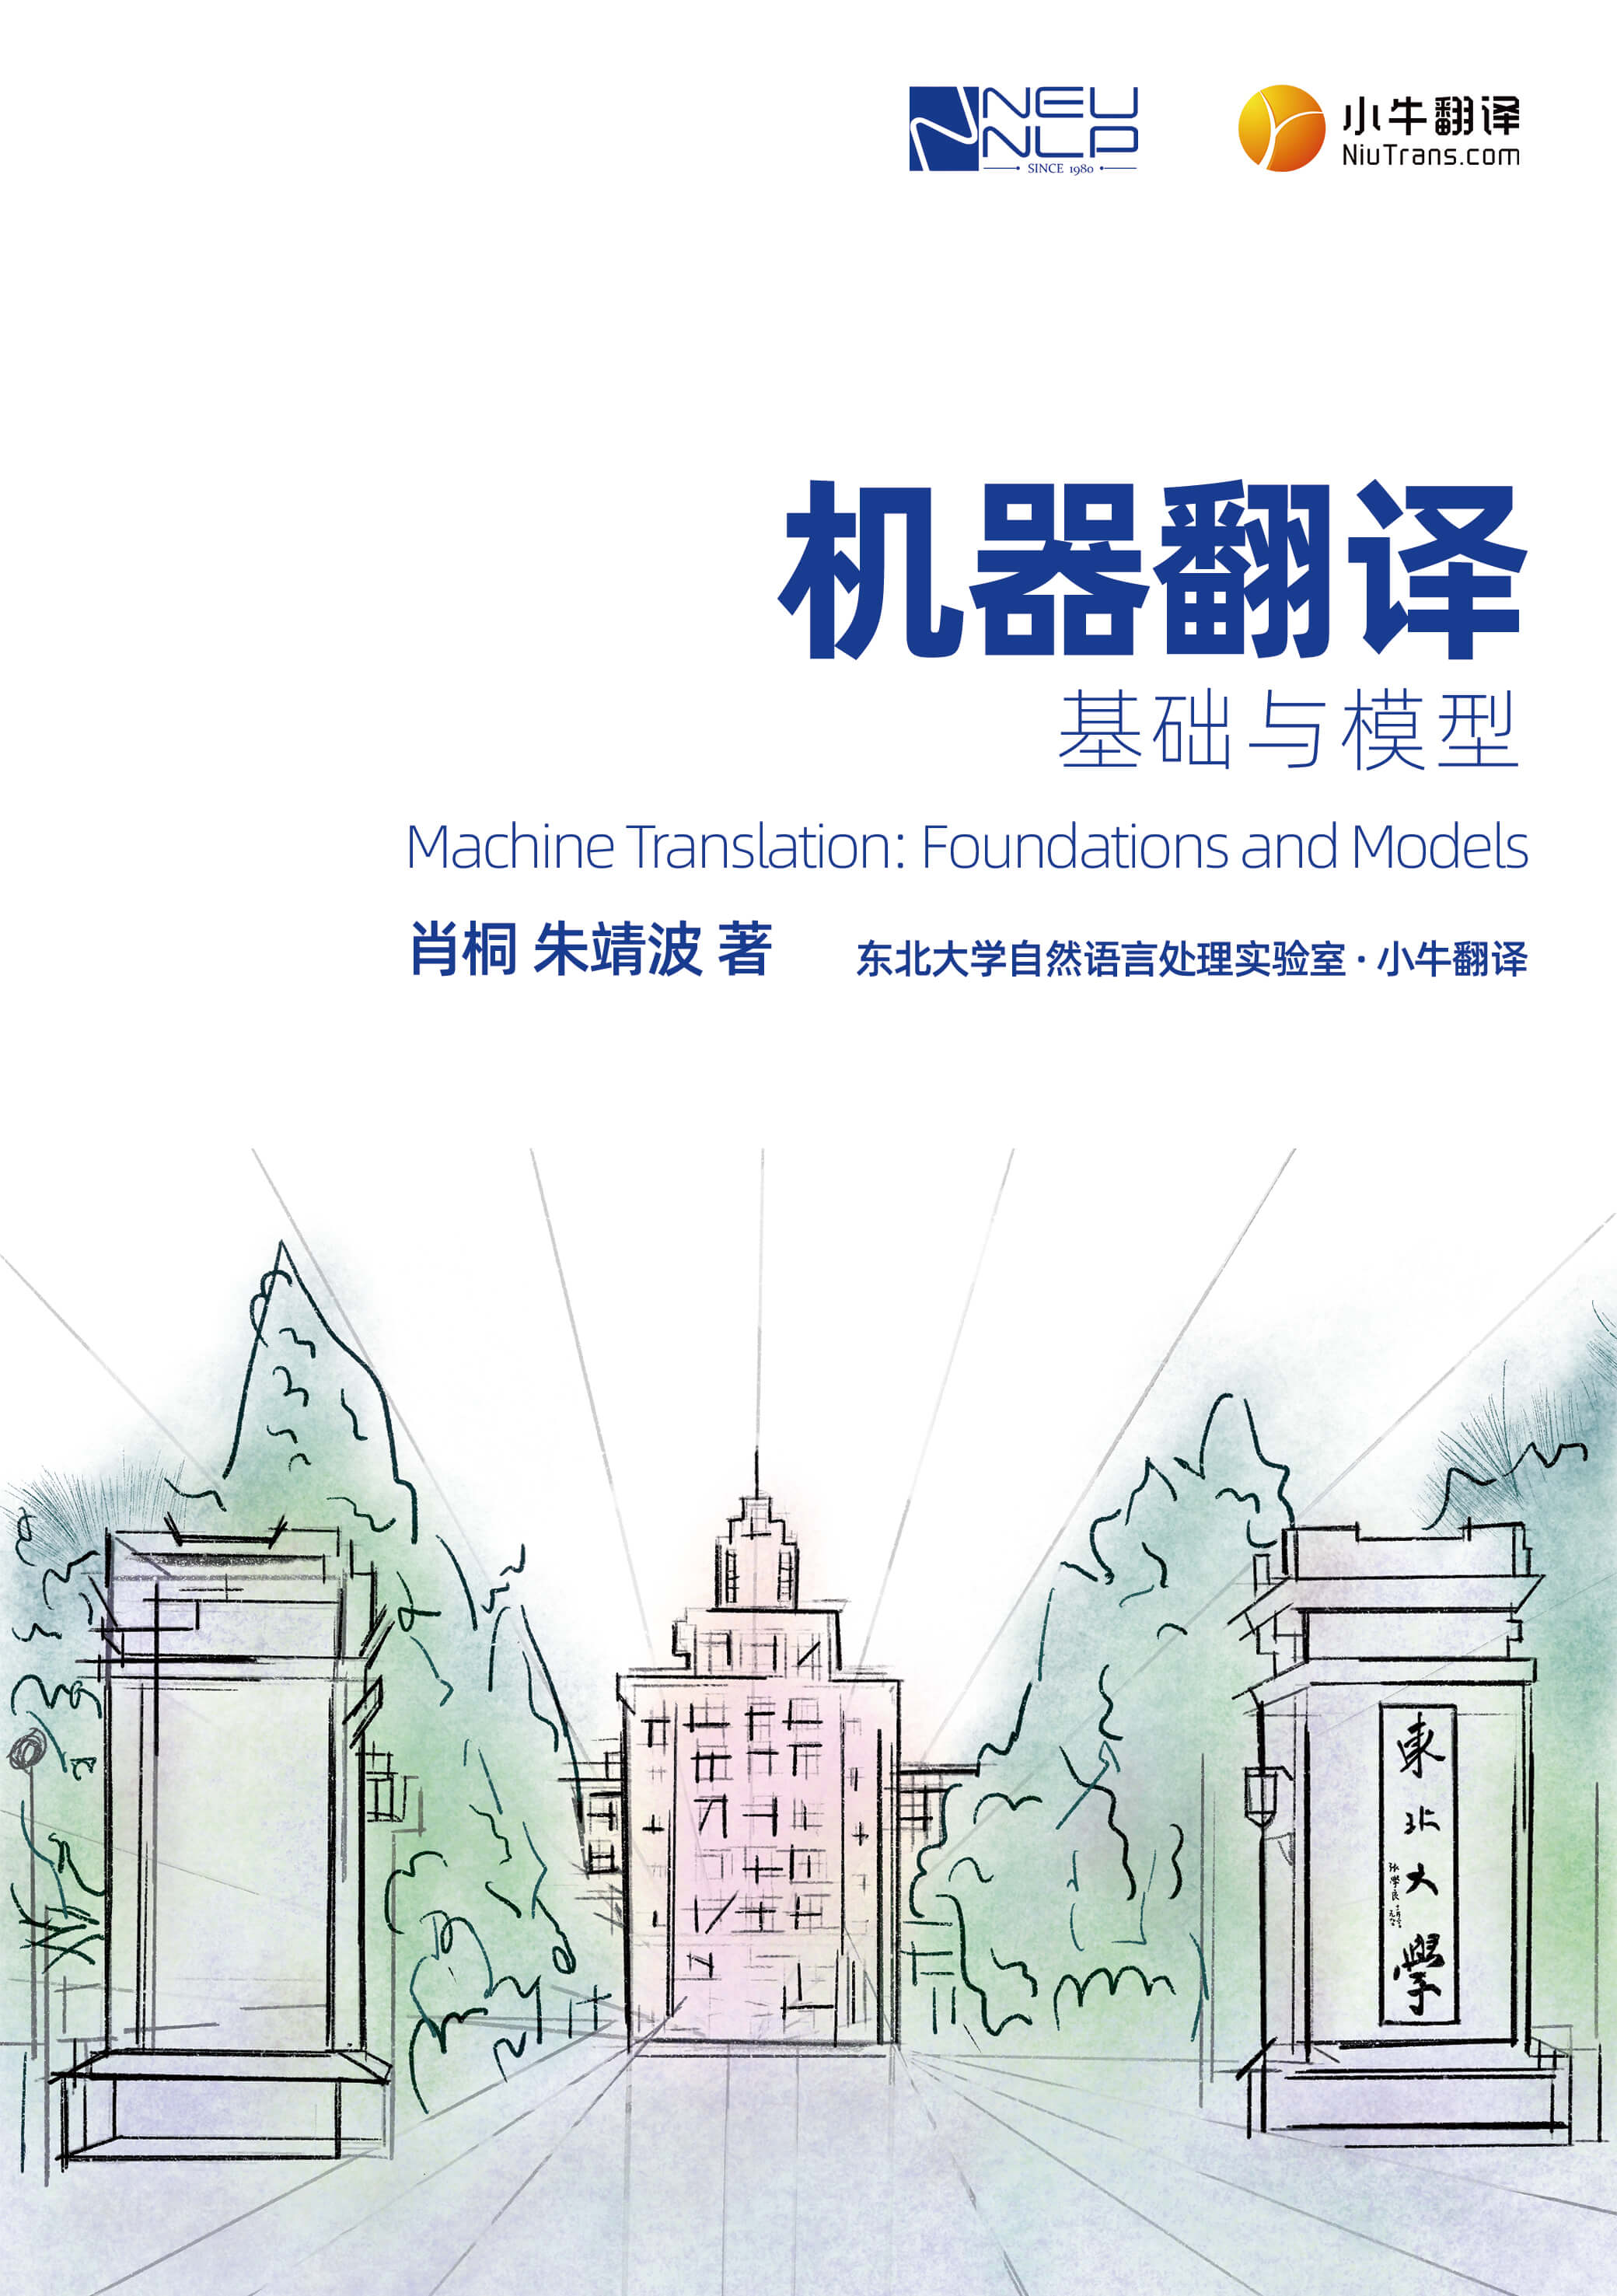
\includegraphics[width=\paperwidth,height=\paperheight]{fig-cover.jpg}};

\end{tikzpicture}
\vfill
\endgroup·

%----------------------------------------------------------------------------------------
%	COPYRIGHT PAGE
%----------------------------------------------------------------------------------------

\newpage
~\vfill
\thispagestyle{empty}

\noindent Copyright \copyright\ 2020 肖桐\ \ 朱靖波\\

\noindent \textsc{东北大学自然语言处理实验室\ $\cdot$\ 小牛翻译}\\

\noindent \textsc{\url{https://opensource.niutrans.com/mtbook/index.html}}\\
\noindent \textsc{\url{https://github.com/NiuTrans/MTBook}}\\

\noindent {\red{Licensed under the Creative Commons Attribution-NonCommercial 4.0 Unported License (the ``License''). You may not use this file except in compliance with the License. You may obtain a copy of the License at \url{http://creativecommons.org/licenses/by-nc/4.0}. Unless required by applicable law or agreed to in writing, software distributed under the License is distributed on an \textsc{``as is'' basis, without warranties or conditions of any kind}, either express or implied. See the License for the specific language governing permissions and limitations under the License.}}\\

\noindent \textit{\today}

%----------------------------------------------------------------------------------------
%	ACKNOWLEDGE PAGE
%----------------------------------------------------------------------------------------

\newpage
~\vfill
\thispagestyle{empty}

{\large
\noindent {\color{red} 在此感谢所有为本书做出贡献的人} \\

\noindent 曹润柘、曾信、孟霞、单韦乔、姜雨帆、王子扬、刘辉、许诺、李北、刘继强、张哲旸、周书含、周涛、张裕浩、李炎洋、林野、陈贺轩、刘晓倩、牛蕊、田丰宁、杜权 \\
}

%----------------------------------------------------------------------------------------
%	PREFACE PAGES
%----------------------------------------------------------------------------------------
\newpage
% !Mode:: "TeX:UTF-8"
% !TEX encoding = UTF-8 Unicode

%----------------------------------------------------------------------------------------
% 机器翻译:统计建模与深度学习方法
% Machine Translation: Statistical Modeling and Deep Learning Methods
%
% Copyright 2020
% 肖桐(xiaotong@mail.neu.edu.cn) 朱靖波 (zhujingbo@mail.neu.edu.cn)
%----------------------------------------------------------------------------------------

\renewcommand\figurename{图}

%----------------------------------------------------------------------------------------
%	PREFACE
%----------------------------------------------------------------------------------------

{\color{white} 空}
\vspace{0.5em}
\begin{center}
{\Huge \bfnew{导\ \ \ \ 读}}
\end{center}
\vspace{2em}

\begin{spacing}{1.18}

让计算机进行自然语言的翻译是人类长期的梦想,也是人工智能的终极目标之一。自上世纪九十年代起,机器翻译迈入了基于统计建模的时代,发展到今天,深度学习等机器学习方法已经在机器翻译中得到了大量的应用,取得了令人瞩目的进步。

在这个时代背景下,对机器翻译的模型、方法和实现技术进行深入了解是自然语言处理领域研究者和实践者所渴望的。本书全面回顾了近三十年内机器翻译的技术发展历程,并围绕统计建模和深度学习两个主题对机器翻译的技术方法进行了全面介绍。在写作中,笔者力求用朴实的语言和简洁的实例阐述机器翻译的基本模型和方法,同时对相关的技术前沿进行讨论。本书可以供计算机相关专业高年级本科生及研究生学习之用,也可以作为自然语言处理,特别是机器翻译领域相关研究人员的参考资料。

本书共分为七个章节,章节的顺序参考了机器翻译技术发展的时间脉络,同时兼顾了机器翻译知识体系的内在逻辑。各章节的主要内容包括:

\begin{itemize}
\vspace{0.5em}
\item 第一章:机器翻译简介
\vspace{0.5em}
\item 第二章:词法、语法及统计建模基础
\vspace{0.5em}
\item 第三章:基于词的机器翻译模型
\vspace{0.5em}
\item 第四章:基于短语和句法的机器翻译模型
\vspace{0.5em}
\item 第五章:人工神经网络和神经语言建模
\vspace{0.5em}
\item 第六章:神经机器翻译模型
\vspace{0.5em}
\item 第七章:神经机器翻译实战 \ \dash \ 参加一次比赛
\vspace{0.5em}
\end{itemize}

其中,第一章是对机器翻译的整体介绍。第二章和第五章是对统计建模和深度学习方法的介绍,分别建立了两个机器翻译范式的基础知识体系 \ \dash \ 统计机器翻译和神经机器翻译。统计机器翻译部分(第三、四章)涉及早期的基于单词的翻译模型,以及本世纪初流行的基于短语和句法的翻译模型。神经机器翻译(第六、七章)代表了当今机器翻译的前沿,内容主要涉及了基于端到端表示学习的机器翻译建模方法。特别地,第七章对一些最新的神经机器翻译方法进行了讨论,为相关科学问题的研究和实用系统的开发提供了可落地的思路。下图展示了本书各个章节及核心概念之间的关系。

{\red 用最简单的方式阐述机器翻译的基本思想}是笔者所期望达到的目标。但是,书中不可避免会使用一些形式化定义和算法的抽象描述,因此,笔者尽所能通过图例进行解释(本书共320张插图)。不过,本书所包含的内容较为广泛,难免会有疏漏,望读者海涵,并指出不当之处。

%-------------------------------------------
\begin{figure}[htp]
\centering
\centering
% !Mode:: "TeX:UTF-8"
% !TEX encoding = UTF-8 Unicode

\begin{tikzpicture}

\tikzstyle{partnode} =[font=\scriptsize,minimum height=2.0em,minimum width=15em,draw,thick,fill=white,drop shadow]
\tikzstyle{secnode} =[font=\footnotesize,minimum height=1.6em,minimum width=14em,align=flush left]

\begin{scope}

% part 1
\node [partnode,anchor=south,blue,minimum height=9.0em,minimum width=22.7em,fill=white] (part1) at ([yshift=-0.5em]0,0) {};
\node [anchor=north] (part1label) at ([yshift=-0.3em]part1.north) {\sffamily\bfseries{机器翻译基础}};
\node [anchor=north west,draw=blue,thick,fill=white,rounded corners] (part1title) at ([xshift=-0.3em,yshift=0.3em]part1.north west) {{\color{blue} {\sffamily\bfseries 第一部分}}};
\node [secnode,anchor=south,fill=ugreen!20,minimum width=21.6em,align=center] (sec01) at (0,0) {第一章\hspace{1em} 机器翻译简介};
\node [secnode,anchor=south west,fill=blue!20] (sec02) at ([yshift=0.8em]sec01.north west) {第二章\hspace{1em} 统计语言建模基础\hspace{3em}};
\node [secnode,anchor=south west,fill=blue!20] (sec03) at ([yshift=0.8em]sec02.north west) {第三章\hspace{1em} 词法分析和语法分析基础};
\node [secnode,anchor=north west,fill=blue!20,minimum width=7em,minimum height=4.1em,align=center] (sec04) at ([xshift=0.6em]sec03.north east) {第四章\\ 翻译质量评价};
\draw [->,very thick] ([yshift=-0.7em]sec02.south) -- ([yshift=-0.1em]sec02.south);
\draw [->,very thick] ([yshift=-0.7em]sec03.south) -- ([yshift=-0.1em]sec03.south);
\draw [->,very thick] ([yshift=-0.7em]sec04.south) -- ([yshift=-0.1em]sec04.south);

% part 2
\node [partnode,anchor=south,orange,minimum height=11.5em,minimum width=18.1em,fill=white] (part2) at ([yshift=3em]part1.north west) {};
\node [anchor=north] (part2label) at ([yshift=-0.3em]part2.north) {\sffamily\bfseries{统计机器翻译}};
\node [anchor=north west,draw=orange,thick,fill=white,rounded corners] (part2title) at ([xshift=-0.3em,yshift=0.3em]part2.north west) {{\color{orange} {\sffamily\bfseries 第二部分}}};
\node [secnode,anchor=south,fill=orange!20,minimum width=17em,align=left] (sec04) at ([yshift=0.5em]part2.south) {第五章\hspace{1em} 基于词的机器翻译建模 \hspace{2.35em}};
\node [secnode,anchor=south,fill=orange!20,minimum width=17em,align=center] (sec05) at ([yshift=0.8em]sec04.north) {\hspace{1.0em}第六章\hspace{1em} 基于扭曲度和繁衍率的模型\hspace{1.6em}};
\node [secnode,anchor=south,fill=orange!20,minimum width=17em,align=center] (sec06) at ([yshift=0.8em]sec05.north) {第七章\hspace{1em} 基于短语的模型 \hspace{5.35em}};
\node [secnode,anchor=south,fill=orange!20,minimum width=17em,align=center] (sec07) at ([yshift=0.8em]sec06.north) {第八章\hspace{1em} 基于句法的模型 \hspace{5.35em}};
\draw [->,very thick] ([yshift=-0.7em]sec05.south) -- ([yshift=-0.1em]sec05.south);
\draw [->,very thick] ([yshift=-0.7em]sec06.south) -- ([yshift=-0.1em]sec06.south);
\draw [->,very thick] ([yshift=-0.7em]sec07.south) -- ([yshift=-0.1em]sec07.south);

% part 3
\node [partnode,anchor=south,red,minimum height=9.5em,minimum width=22.7em,fill=white] (part3) at ([yshift=3em,xshift=2.5em]part2.north east) {};
\node [anchor=north] (part3label) at ([yshift=-0.3em]part3.north) {\sffamily\bfseries{神经机器翻译}};
\node [anchor=north west,draw=red,thick,fill=white,rounded corners] (part3title) at ([xshift=-0.3em,yshift=0.3em]part3.north west) {{\color{red} {\sffamily\bfseries 第三部分}}};
\node [secnode,anchor=south,fill=magenta!20,minimum width=21.6em,align=center] (sec09) at ([yshift=0.5em]part3.south) {第九章\hspace{1em} 人工神经网络和神经语言建模};
\node [secnode,anchor=south west,fill=red!20,minimum width=6.6em,minimum height=4.5em,align=center] (sec10) at ([yshift=0.8em]sec09.north west) {第十章\\ 基于循环神经 \\ 网络的模型};
\node [secnode,anchor=south west,fill=red!20,minimum width=6.6em,minimum height=4.5em,align=center] (sec11) at ([xshift=0.8em]sec10.south east) {第十一章\\ 基于卷积神经 \\ 网络的模型};
\node [secnode,anchor=south west,fill=red!20,minimum width=6.6em,minimum height=4.5em,align=center] (sec12) at ([xshift=0.8em]sec11.south east) {第十二章\\ 基于自注意力 \\ 的模型};
\draw [->,very thick] ([yshift=-0.7em]sec10.south) -- ([yshift=-0.1em]sec10.south);
\draw [->,very thick] ([yshift=-0.7em]sec11.south) -- ([yshift=-0.1em]sec11.south);
\draw [->,very thick] ([yshift=-0.7em]sec12.south) -- ([yshift=-0.1em]sec12.south);


% part 4
\node [partnode,anchor=south,ugreen,minimum height=12.0em,minimum width=29.7em,fill=white] (part4) at ([yshift=3em,xshift=6em]part3.north west) {};
\node [anchor=north] (part4label) at ([yshift=-0.3em]part4.north) {\sffamily\bfseries{机器翻译前沿}};
\node [anchor=north west,draw=ugreen,thick,fill=white,rounded corners] (part4title) at ([xshift=-0.3em,yshift=0.3em]part4.north west) {{\color{ugreen} {\sffamily\bfseries 第四部分}}};
\node [secnode,anchor=south west,fill=cyan!20,minimum width=14.0em,align=center] (sec13) at ([yshift=0.5em,xshift=0.5em]part4.south west) {第十三章\hspace{1em} 神经机器翻译模型训练};
\node [secnode,anchor=west,fill=cyan!20,minimum width=14.0em,align=center] (sec14) at ([xshift=0.6em]sec13.east) {第十四章\hspace{1em} 神经机器翻译模型推断};
\node [secnode,anchor=south west,fill=green!30,minimum width=9em,minimum height=4.5em,align=center] (sec15) at ([yshift=0.8em]sec13.north west) {第十五章\\ 神经机器翻译 \\ 结构优化};
\node [secnode,anchor=south west,fill=green!30,minimum width=9em,minimum height=4.5em,align=center] (sec16) at ([xshift=0.8em]sec15.south east) {第十六章\\ 低资源 \\ 神经机器翻译};
\node [secnode,anchor=south west,fill=green!30,minimum width=9em,minimum height=4.5em,align=center] (sec17) at ([xshift=0.8em]sec16.south east) {第十七章\\ 多模态、多层次 \\ 机器翻译};
\node [secnode,anchor=south west,fill=amber!25,minimum width=28.7em,align=center] (sec18) at ([yshift=0.8em]sec15.north west) {第十八章\hspace{1em} 机器翻译应用技术};
\node [rectangle,draw,dotted,thick,inner sep=0.1em,fill opacity=1] [fit = (sec13) (sec14)] (nmtbasebox) {};
\draw [->,very thick] ([yshift=-0.7em]sec15.south) -- ([yshift=-0.1em]sec15.south);
\draw [->,very thick] ([yshift=-0.7em]sec16.south) -- ([yshift=-0.1em]sec16.south);
\draw [->,very thick] ([yshift=-0.7em]sec17.south) -- ([yshift=-0.1em]sec17.south);
\draw [<-,very thick] ([yshift=0.7em]sec15.north) -- ([yshift=0.1em]sec15.north);
\draw [<-,very thick] ([yshift=0.7em]sec16.north) -- ([yshift=0.1em]sec16.north);
\draw [<-,very thick] ([yshift=0.7em]sec17.north) -- ([yshift=0.1em]sec17.north);
\draw [->,very thick,dotted] ([yshift=-0.7em,xshift=0.4em]sec15.south east) -- ([yshift=0.7em,xshift=0.4em]sec15.north east);
\draw [->,very thick,dotted] ([yshift=-0.7em,xshift=0.4em]sec16.south east) -- ([yshift=0.7em,xshift=0.4em]sec16.north east);

% lines and arrows
\draw [->,line width=0.2em] ([xshift=-0.1em]part1.west) .. controls +(west:5em) and +(south:3em) .. ([yshift=-0.1em,xshift=-5em]part2.south);
\draw [->,line width=0.2em] ([xshift=-2em,yshift=0.1em]part1.north east) -- ([xshift=-2em,yshift=17.3em]part1.north east);
\draw [->,line width=0.2em] ([xshift=0.3em,yshift=-2em]part2.east) .. controls +(east:6em) and +(south:4em) .. ([yshift=-0.3em,xshift=4em]part3.south);
\draw [->,line width=0.2em] ([xshift=-5em,yshift=0.5em]part2.north) -- ([xshift=-5em,yshift=15.3em]part2.north);
\draw [->,line width=0.2em] ([xshift=4em,yshift=0.1em]part3.north) -- ([xshift=4em,yshift=2.7em]part3.north);

\end{scope}

\end{tikzpicture}

\end{figure}
%-------------------------------------------

\end{spacing}










%----------------------------------------------------------------------------------------
%	TABLE OF CONTENTS
%----------------------------------------------------------------------------------------
%\usechapterimagefalse % If you don't want to include a chapter image, use this to toggle images off - it can be enabled later with \usechapterimagetrue
\chapterimage{fig-NEU-1.jpg} % Image of the content page
\pagestyle{empty} % Disable headers and footers for the following pages
\tableofcontents % Show contents
\cleardoublepage % Place the first page of each chapter on odd pages
\pagestyle{fancy} % Enable headers and footers


%----------------------------------------------------------------------------------------
%	CHAPTERS
%----------------------------------------------------------------------------------------

% !Mode:: "TeX:UTF-8"
% !TEX encoding = UTF-8 Unicode

%----------------------------------------------------------------------------------------
% 机器翻译:统计建模与深度学习方法
% Machine Translation: Statistical Modeling and Deep Learning Methods
%
% Copyright 2020
% 肖桐(xiaotong@mail.neu.edu.cn) 朱靖波 (zhujingbo@mail.neu.edu.cn)
%----------------------------------------------------------------------------------------

%----------------------------------------------------------------------------------------
%    CONFIGURATIONS
%----------------------------------------------------------------------------------------

\part{机器翻译基础}
\renewcommand\figurename{图}%将figure改为图
\renewcommand\tablename{表}%将figure改为图
\chapterimage{fig-NEU-2.jpg} % Chapter heading image

%----------------------------------------------------------------------------------------
%	CHAPTER 1
%----------------------------------------------------------------------------------------

\chapter{机器翻译简介}

%----------------------------------------------------------------------------------------
%    NEW SECTION
%----------------------------------------------------------------------------------------

\section{机器翻译的概念}

\parinterval 从广义上来讲,“翻译”是指把一个事物转化为另一个事物的过程。这个概念多使用在对序列的转化上,比如,计算机程序的编译、自然语言文字的翻译、生物蛋白质的合成等。在程序编译中,高级语言编写的程序经过一系列的处理后转化为可执行的目标程序,这是一种从高级程序语言到低级程序语言的“翻译”。在人类语言的翻译中,一种语言文字通过人脑转化为另一种语言表达,这是一种自然语言的“翻译”。在蛋白质合成的第一步,RNA分子序列转化为特定的氨基酸序列,这是一种生物学遗传信息的“翻译”。甚至说给上联对出下联、给一幅图片写出图片的主题等都可以被看作是“翻译”的过程。
\vspace{0.5em}

\parinterval 这里更加关注人类语言之间的翻译问题,即自然语言的翻译。如图\ref{fig:1-1}所示,通过计算机可以将一段汉语文字自动转化为英语文字,汉语被称为{\small\bfnew{源语言}}\index{源语言}(Source Language)\index{Source Language},英语被称为{\small\bfnew{目标语言}}\index{目标语言}(Target Language)\index{Target Language}。

%----------------------------------------------
\begin{figure}[htp]
    \centering
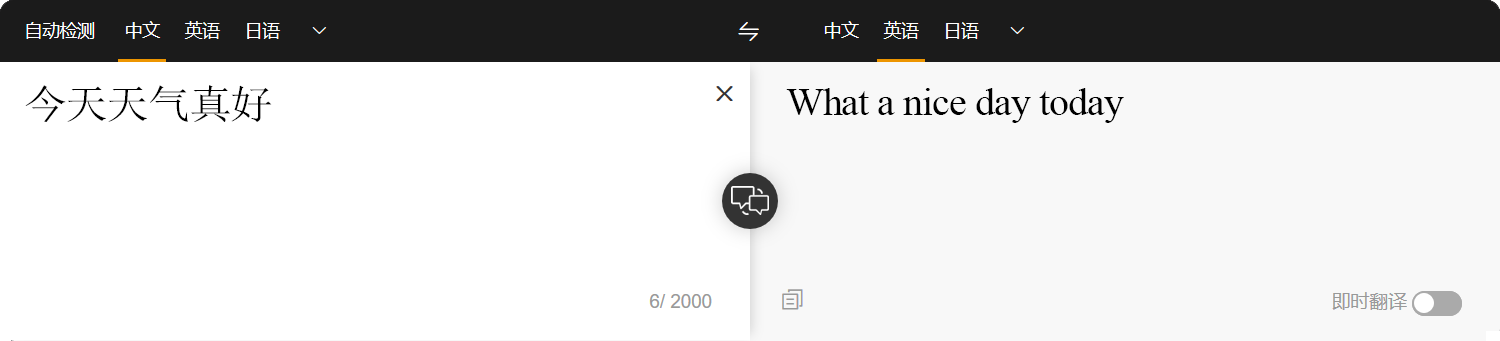
\includegraphics[scale=0.2]{./Chapter1/Figures/figure-zh_en-example.png}
    \caption{通过计算机将汉语翻译为英语}
    \label{fig:1-1}
\end{figure}
%----------------------------------------------

\parinterval 一直以来,文字的翻译往往是由人完成。让计算机像人一样进行翻译似乎还是电影中的桥段,因为很难想象语言的多样性和复杂性可以用计算机语言进行描述。但是时至今日,人工智能技术的发展已经大大超越了人类传统的认知,用计算机进行自动翻译也不再是一种梦想,它已经深入到人们生活的很多方面,并发挥着重要作用。而这种由计算机进行自动翻译的过程也被称作{\small\bfnew{机器翻译}}\index{机器翻译}(Machine Translation)\index{Machine Translation}。类似地,自动翻译、智能翻译、多语言自动转换等概念也是指同样的事情。如果将今天的机器翻译和人工翻译进行对比,可以发现机器翻译系统所生成的译文还不够完美,甚至有时翻译质量非常差,但是它的生成速度快且成本低廉,更为重要的是机器翻译系统可以从大量数据中不断学习和进化。

\parinterval 人工翻译尽管精度很高,但是费时费力。当需要翻译大量的文本且精度要求不那么高时,比如海量数据的浏览型任务,机器翻译的优势就体现出来了。对于人工作业无法完成的事情,使用机器翻译可能只需花费几个小时甚至几分钟就能完成。这就类似于拿着锄头耕地种庄稼和使用现代化机器作业之间的区别。

\parinterval 实现机器翻译往往需要多个学科知识的融合,如数学、语言学、计算机科学、心理学等等。而最终呈现给使用者的是一套软件系统\ \dash\ 机器翻译系统。通俗来讲,机器翻译系统就是一个可以在计算机上运行的软件工具,与人们使用的其他软件一样,只不过机器翻译系统是由“不可见的程序”组成。虽然这个系统非常复杂,但是呈现出来的形式却很简单,比如输入是待翻译的句子或文本,输出是译文句子或文本。

\parinterval 用机器进行翻译的想法可以追溯到电子计算机产生之前,发展过程中也经历了多个范式的变迁,现代机器翻译系统大多是基于数据驱动的方法\ \dash\ 从数据中自动学习翻译知识,并运用这些知识对新的文本进行翻译。

\parinterval 从机器翻译系统的组成上来看,通常可以抽象为两个部分,如图\ref{fig:1-2}所示:

\begin{itemize}
\vspace{0.5em}
\item {\small\bfnew{资源}}:如果把机器翻译系统比作一辆汽车,资源就好比是可以使汽车运行的“汽油”,它包括很多内容,如翻译规则、双(单)语数据、知识库等翻译知识,且这些“知识”都是计算机可读的。值得一提的是,如果没有翻译资源的支持,任何机器翻译系统都无法运行起来。
\vspace{0.5em}
\item {\small\bfnew{系统}}:机器翻译算法的程序实现被称作系统,也就是机器翻译研究人员开发的软件。无论是翻译规则、翻译模板还是统计模型中的参数都需要通过机器翻译系统进行读取和使用。
\vspace{0.5em}
\end{itemize}

%----------------------------------------------
\begin{figure}[htp]
    \centering
\definecolor{ublue}{rgb}{0.152,0.250,0.545}
\definecolor{ugreen}{rgb}{0,0.5,0}
\begin{tikzpicture}
\node [thick,rounded corners=3mm,draw=blue!50!black!50,top color=white,bottom color=blue!50!black!20] (s) at (0,0) {输入文字};
\node [thick,minimum width=6em,minimum height=3em,draw=red!50!black!50,anchor=west] (mt) at ([xshift=0.5in]s.east) {};
\node [thick,minimum width=6em,minimum height=1.5em,draw=red!50!black!50,top color=white,bottom color=red!50!black!20,anchor=north] (mt1) at (mt.north) {机器翻译};
\node [thick,rounded corners=3mm,draw=blue!50!black!50,top color=white,bottom color=blue!50!black!20,anchor=west] (t) at ([xshift=0.5in]mt.east) {输出译文};
{
\node [draw=ugreen,fill=ugreen,minimum width=3.1em,minimum height=1.5em,anchor=south west] (part1) at (mt.south west) {{\color{white} 1}};
\node [draw=ublue,fill=ublue,minimum width=3.1em,minimum height=1.5em,anchor=south east] (part2) at (mt.south east) {{\color{white} 2}};
}
\draw[-latex,thick] (s.east)--(mt.west);
\draw[-latex,thick] (mt.east)--(t.west);

{
\begin{scope}[yshift=-1.0in]
\node [] (part1label) at (0,0) {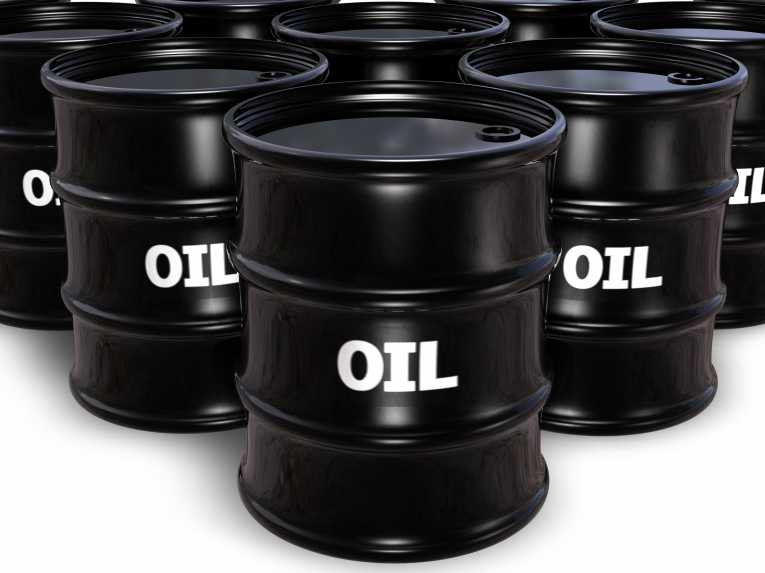
\includegraphics[scale=0.10]{./Chapter1/Figures/figure-oil.jpg}};
\node [anchor=north west] (part1text) at ([xshift=-1em,yshift=0.0em]part1label.south west) {\begin{tabular}{l}{\color{red}{资源}}:可以使机器翻译\\系统运行的``汽油''\end{tabular}};
\end{scope}
}

{
\begin{scope}[yshift=-1.0in,xshift=2.8in]
\node [] (part2label) at (0,0) {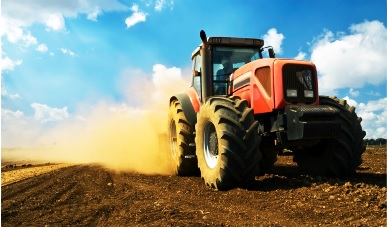
\includegraphics[scale=0.33]{./Chapter1/Figures/figure-truck.jpg}};
\node [anchor=north west] (part2text) at ([xshift=-1em,yshift=0em]part2label.south west) {\begin{tabular}{l}{\color{red}{系统}}:利用资源完成\\自动翻译的程序\end{tabular}};
\end{scope}
}

{
\draw[<-,thick] (part1label.north)..controls +(north:0.6) and +(south:0.6)..([yshift=0.2em]part1.south);
}

{
\draw[<-,thick] ([yshift=0.0em]part2label.north)..controls +(north:0.6) and +(south:0.6)..([yshift=0.2em]part2.south);
}

\end{tikzpicture}



    \caption{机器翻译系统的组成}
    \label{fig:1-2}
\end{figure}
%-------------------------------------------

\parinterval 构建一个强大的机器翻译系统需要“资源”和“系统”两方面共同作用。在资源方面,随着语料库语言学的发展,已经有大量的高质量的双语和单语数据(称为语料)被整理并且被电子化存储,因此可以说具备了研发机器翻译系统所需要的语料基础。特别是像英语、汉语等世界主流语种,相关语料资源已经非常丰富,这也大大加速了相关研究的进展。当然,对于一些稀缺资源语种或者特殊的领域,语料库中的语料仍然匮乏,但是这些并不影响机器翻译领域整体的发展速度。因此在现有语料库的基础上,很多研究者把精力集中在“系统”研发上。

%----------------------------------------------------------------------------------------
%    NEW SECTION
%----------------------------------------------------------------------------------------

\sectionnewpage
\section{机器翻译简史}

\parinterval 虽然翻译这个概念在人类历史中已经存在了上千年,但机器翻译发展至今只有七十余年的历史。纵观机器翻译的发展,历程曲折又耐人寻味,可以说,回顾机器翻译的历史对深入理解相关技术方法会有很好的启发,甚至对了解整个自然语言处理领域的发展也有启示作用。

%----------------------------------------------------------------------------------------
%    NEW SUB-SECTION
%----------------------------------------------------------------------------------------

\subsection{人工翻译}

\parinterval 人类形成语言文字的过程中逐渐形成了翻译的概念。一个著名的标志性证据是罗塞塔石碑(Rosetta Stone),如图\ref{fig:1-3}所示。这个石碑制作于公元前196年,据说是可供考证的最久远的记载平行文字的历史遗迹。石碑由上至下刻有同一段埃及国王诏书的三种语言版本,最上面是古埃及象形文,中间是埃及草书,最下面是古希腊文。可以明显看出石碑上中下雕刻的文字的纹理是不同的。尽管用不同的语言文字描述同一件事在今天看来很常见,但是这在生产力低下的两千年前是很罕见的。很多人认为罗塞塔石碑是标志翻译或人工翻译的一个起点。目前罗塞塔石碑保存于大英博物馆,并成为该馆最具代表性的镇馆之宝之一。

%----------------------------------------------
\begin{figure}[htp]
    \centering
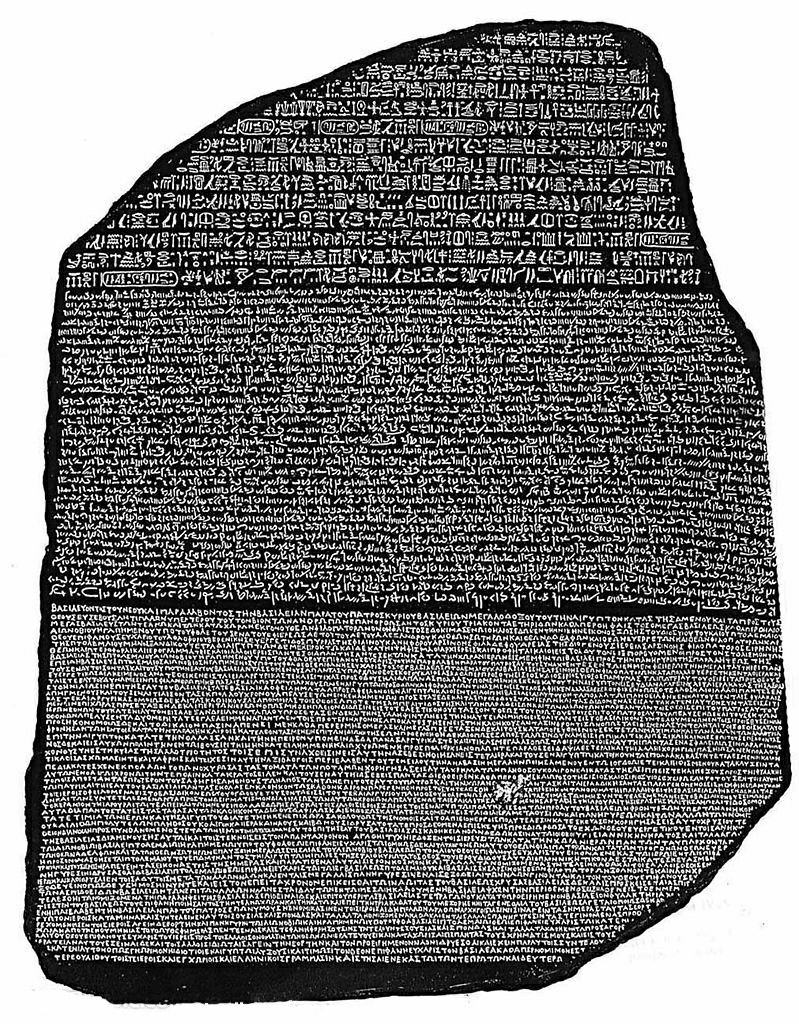
\includegraphics[scale=0.20]{./Chapter1/Figures/figure-rosetta-stone.jpg}
    \caption{罗塞塔石碑}
    \label{fig:1-3}
\end{figure}
%------------------------------------------

\parinterval 在此之后,更多的翻译工作在文化和知识传播中开展。其中一个典型代表是宗教文献的翻译。宗教是人类意识形态的一个重要载体,为了宣传教义,人们编写了大量的宗教文献。在西方,一项最早被记录的翻译活动是将旧约圣经(希伯来文及埃兰文)翻译为希腊文版本。迄今为止人类历史上翻译版本最多的书就是圣经。在中国唐代,有一位世界性的文化人物\ \dash \ 玄奘,他不仅是佛学家、旅行家,还是翻译家。玄奘西行求法归来后把全部的心血和智慧奉献给了译经事业,在助手们的帮助下,共翻译佛教经论74部,1335卷,每卷万字左右,合计1335万字,占去整个唐代译经总数的一半以上\upcite{慧立2000大慈恩寺三藏法師傳},树立了我国古代翻译思想的光辉典范。

\parinterval 翻译在人类历史长河中起到了重要的作用。一方面,由于语言文字、文化和地理位置的差异性,使得翻译成为一个重要的需求;另一方面,翻译也加速了不同文明的融会贯通,促进了世界的发展。今天,翻译已经成为重要的行业之一,包括各个高校也都设立了翻译及相关专业,相关人才不断涌现。据《2019年中国语言服务行业发展报告》\upcite{2019cns}统计:全球语言服务产值预计将首次接近500亿美元;中国涉及语言服务的在营企业360,000余家,语言服务为主营业务的在营企业近万家,总产值超过300亿元,年增长3\%以上;全国开设外语类专业的高校数量多达上千所,其中设立有翻译硕士(MTI)和翻译本科(BTI)专业的院校分别有250余所和280余所,其中仅MTI的累计招生数就高达6万余人\upcite{赵军峰2019深化改革}。当然,面对着巨大的需求,如何使用机器辅助翻译等技术手段提高人工翻译效率,也是人工翻译和机器翻译领域需要共同探索的方向。

%----------------------------------------------------------------------------------------
%    NEW SUB-SECTION
%----------------------------------------------------------------------------------------

\subsection{机器翻译的萌芽}

\parinterval 人工翻译已经存在了上千年,而机器翻译又起源于什么时候呢?机器翻译跌宕起伏的发展史可以分为萌芽期、受挫期、快速成长期和爆发期四个阶段。

\parinterval 早在17世纪,如Descartes、Leibniz、Cave\ Beck、Athanasius\ Kircher和Johann\ Joachim\ Becher等很多学者就提出采用机器词典(电子词典)来克服语言障碍的想法\upcite{knowlson1975universal},这种想法在当时是很超前的。随着语言学、计算机科学等学科的发展,在19世纪30年代使用计算模型进行自动翻译的思想开始萌芽,如当时法国科学家Georges Artsrouni就提出用机器来进行翻译的想法。只是那时依然没有合适的实现手段,所以这种想法的合理性无法被证实。

\parinterval 随着第二次世界大战爆发, 对文字进行加密和解密成为重要的军事需求,这也使得数学和密码学变得相当发达。在战争结束一年后,世界上第一台通用电子数字计算机于1946年研制成功,至此使用机器进行翻译有了真正实现的可能。

\parinterval 基于战时密码学领域与通讯领域的研究,Claude Elwood Shannon在1948年提出使用“噪声信道”描述语言的传输过程,并借用热力学中的“{\small\bfnew{熵}}\index{熵}”(Entropy)\index{Entropy}来刻画消息中的信息量\upcite{DBLP:journals/bstj/Shannon48}。次年,Shannon与Warren Weaver更是合著了著名的\emph{The Mathematical Theory of Communication}\upcite{shannon1949the},这些工作都为后期的统计机器翻译打下了理论基础。

\parinterval 1949年,Weaver撰写了一篇名为\emph{TRANSLATION}的备忘录\upcite{weaver1955translation},在这个备忘录中Weaver提出用密码学的方法解决人类语言翻译任务的想法,比如把汉语看成英语的一个加密文本,那么将汉语翻译成英语就类似于解密的过程。并且在这篇备忘录中第一次提出了机器翻译,正式开创了机器翻译的概念,这个概念一直沿用至今。虽然,在那个年代进行机器翻译的研究条件并不成熟,包括使用加密解密技术进行自动翻译的很多尝试很快也被验证是不可行的,但是这些早期的探索为后来机器翻译的发展提供了思想的火种。

%----------------------------------------------------------------------------------------
%    NEW SUB-SECTION
%----------------------------------------------------------------------------------------

\subsection{机器翻译的受挫}

\parinterval 随着电子计算机的发展,研究者开始尝试使用计算机来进行自动翻译。1954年,美国乔治敦大学在IBM公司支持下,启动了第一次真正的机器翻译实验。翻译的目标是将几个简单的俄语句子翻译成为英语,翻译系统包含6条翻译规则和250词汇。这次翻译实验中测试了50个化学文本句子,取得了初步成功。在某种意义上来说,这个实验显示了采用基于词典和翻译规则的方法可以实现机器翻译过程。虽然只是取得了初步成功,但却引起了苏联、英国和日本研究机构的机器翻译研究热,大大推动了早期机器翻译的研究进展。

\parinterval 1957年,Noam Chomsky在\emph{Syntactic Structures}中描述了转换生成语法\upcite{chomsky1957syntactic},并使用数学方法来研究自然语言,建立了包括上下文有关语法、上下文无关语法等4种类型的语法。这些工作最终为今天计算机中广泛使用的“形式语言”奠定了基础。而他的思想也深深地影响了同时期的语言学和自然语言处理领域的学者。特别的是,早期基于规则的机器翻译中也大量使用了这些思想。

\parinterval 虽然在这段时间,使用机器进行翻译的议题越加火热,但是事情并不总是一帆风顺,怀疑论者对机器翻译一直存有质疑,并很容易找出一些机器翻译无法解决的问题。自然地,人们也期望能够客观地评估一下机器翻译的可行性。当时美国基金资助组织委任自动语言处理咨询会承担了这项任务。经过近两年的调查与分析,该委员会于1966年11月公布了一个题为\emph{LANGUAGE AND MACHINES}的报告(图\ref{fig:1-5}),即ALPAC报告。该报告全面否定了机器翻译的可行性,为机器翻译的研究泼了一盆冷水。

%----------------------------------------------
\begin{figure}[htp]
    \centering
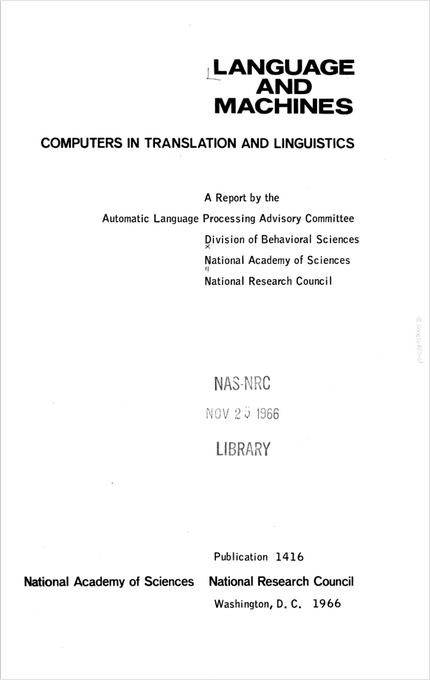
\includegraphics[scale=0.65]{./Chapter1/Figures/figure-report.jpg}
    \caption{ALPAC报告}
    \label{fig:1-4}
\end{figure}
%-------------------------------------------

\parinterval 随后美国政府终止了对机器翻译研究的支持,这导致整个产业界和学术界都开始回避机器翻译。没有了政府的支持,企业也无法进行大规模投入,机器翻译的研究就此受挫。

\parinterval 从历史上看,包括机器翻译在内,很多人工智能领域在那个年代并不受“待见”,其主要原因在于当时的技术水平还比较低,而大家又对机器翻译等技术的期望过高。最后发现,当时的机器翻译水平无法满足实际需要,因此转而排斥它。但是,也正是这一盆冷水,让研究人员可以更加冷静地思考机器翻译的发展方向,为后来的爆发蓄力。

%----------------------------------------------------------------------------------------
%    NEW SUB-SECTION
%----------------------------------------------------------------------------------------

\subsection{机器翻译的快速成长}

\parinterval 事物的发展都是螺旋式上升的,机器翻译也是一样。早期基于规则的机器翻译方法需要人来书写规则,虽然对少部分句子具有较高的翻译精度,可是对翻译现象的覆盖度有限,而且对规则或者模板中的噪声非常敏感,系统健壮性差。

\parinterval 上世纪70年代中后期,特别是80年代到90年代初,国家之间往来日益密切,而不同语言之间形成的交流障碍愈发严重,传统的人工作业方式已经远远不能满足需求。与此同时,语料库语言学的发展也为机器翻译提供了新的思路。一方面,随着传统纸质文字资料不断电子化,计算机可读的语料越来越多,这使得人们可以用计算机对语言规律进行统计分析。另一方面,随着可用数据越来越多,用数学模型描述这些数据中的规律并进行推理逐渐成为可能。这也衍生出一类数学建模方法\ \dash\ {\small\bfnew{数据驱动}}\index{数据驱动}(Data-driven)\index{Data-driven}的方法。同时这类方法也成为了随后出现的统计机器翻译的基础,比如,IBM研究人员提出的基于噪声信道模型的5种统计翻译模型\upcite{brown1990statistical,DBLP:journals/coling/BrownPPM94}。

\parinterval 基于数据驱动的方法不依赖于人书写的规则,机器翻译的建模、训练和推断都可以自动地从数据中学习。这使得整个机器翻译的范式发生了翻天覆地的变化,比如,日本学者长尾真提出的基于实例的方法\upcite{nagao1984framework,DBLP:conf/coling/SatoN90}和统计机器翻译\upcite{brown1990statistical,DBLP:journals/coling/BrownPPM94}就是在此期间兴起的。此外,这样的方法使得机器翻译系统的开发代价大大降低。

\parinterval 从上世纪90年代到本世纪初,随着语料库的完善与高性能计算机的发展,统计机器翻译很快成为了当时机器翻译研究与应用的代表性方法。一个标志性的事件是谷歌公司推出了一个在线的免费自动翻译服务,也就是大家熟知的谷歌翻译。这使得机器翻译这种“高大上”的技术快速进入人们的生活,而不再是束之高阁的科研想法。随着机器翻译不断走向实用,机器翻译的应用也越来越多,这反过来促进了机器翻译的研究进程。比如,在2005-2015年间,统计机器翻译这个主题几乎统治了ACL等自然语言处理相关方向顶级会议的论文,可见其在当时的影响力。

%----------------------------------------------------------------------------------------
%    NEW SUB-SECTION
%----------------------------------------------------------------------------------------

\subsection{机器翻译的爆发}

\parinterval 进入二十一世纪,统计机器翻译拉开了黄金发展期的序幕。在这一时期,各种基于统计机器翻译模型层出不穷,经典的基于短语的模型和基于句法的模型也先后被提出。在2013年以后,机器学习的进步带来了机器翻译技术的进一步提升。特别是基于神经网络的深度学习方法在机器视觉、语音识别中被成功应用,带来性能的飞跃式提升。很快,深度学习方法也被用于机器翻译。

\parinterval 实际上,对于机器翻译任务来说,深度学习方法被广泛使用也是一种必然,原因如下:

\begin{itemize}
\vspace{0.5em}
\item 第一,端到端学习不依赖于过多的先验假设。在统计机器翻译时代,模型设计或多或少会对翻译的过程进行假设,称为隐藏结构假设。比如基于短语的模型假设:源语言和目标语言都会被切分成短语序列,这些短语之间存在某种对齐关系。这种假设既有优点也有缺点:一方面,该假设有助于模型融入人类的先验知识,比如,统计机器翻译中一些规则的设计就借鉴了语言学的相关概念;另一方面,假设越多模型受到的限制也越多。如果假设是正确的,模型可以很好地描述问题。但如果假设错误,那么模型就可能产生偏差。深度学习不依赖于先验知识,也不需要手工设计特征,模型直接从输入和输出的映射上进行学习(端到端学习),这样也在一定程度上避免了隐藏结构假设造成的偏差。
\vspace{0.5em}
\item 第二,神经网络的连续空间模型有更强的表示能力。机器翻译中的一个基本问题是:如何表示一个句子?统计机器翻译把句子的生成过程看作是短语或者规则的推导,这本质上是一个离散空间上的符号系统。深度学习把传统的基于离散化的表示变成了连续空间的表示。比如,用实数空间的分布式表示代替了离散化的词语表示,而整个句子可以被描述为一个实数向量。这使得翻译问题可以在连续空间上描述,进而大大缓解了传统离散空间模型维度灾难等问题。更重要的是,连续空间模型可以用梯度下降等方法进行优化,具有很好的数学性质并且易于实现。
\vspace{0.5em}
\item 第三,深度网络学习算法的发展和GPU\index{GPU}(Graphics Processing Unit)\index{Graphics Processing Unit}等并行计算设备为训练神经网络提供了可能。早期的基于神经网络的方法一直没有在机器翻译甚至自然语言处理领域得到大规模应用,其中一个重要的原因是这类方法需要大量的浮点运算,但是以前计算机的计算能力无法达到这个要求。随着GPU等并行计算设备的进步,训练大规模神经网络也变为了可能。现在已经可以在几亿、几十亿,甚至上百亿句对上训练机器翻译系统,系统研发的周期越来越短,进展日新月异。
\vspace{0.5em}
\end{itemize}

\parinterval 今天,神经机器翻译已经成为新的范式,与统计机器翻译一同推动了机器翻译技术与应用产品的发展。比如,从世界上著名的机器翻译比赛WMT和CCMT中就可以看出这个趋势。如图\ref{fig:1-5}所示,其中左图是WMT\ 19国际机器翻译比赛的参赛队伍的截图,这些参赛队伍基本上都在使用深度学习完成机器翻译的建模。而在WMT\ 19各个项目夺冠系统中(\ref{fig:1-5}右图),神经机器翻译也占据了主导地位。

%----------------------------------------------
\begin{figure}[htp]
    \centering
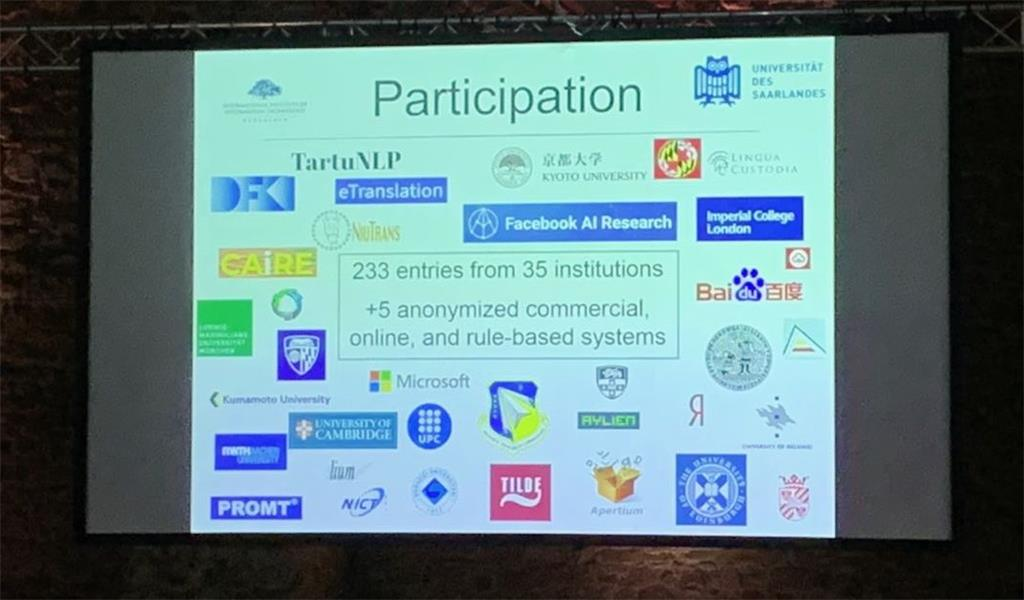
\includegraphics[scale=0.3]{./Chapter1/Figures/figure-wmt-participation.jpg}
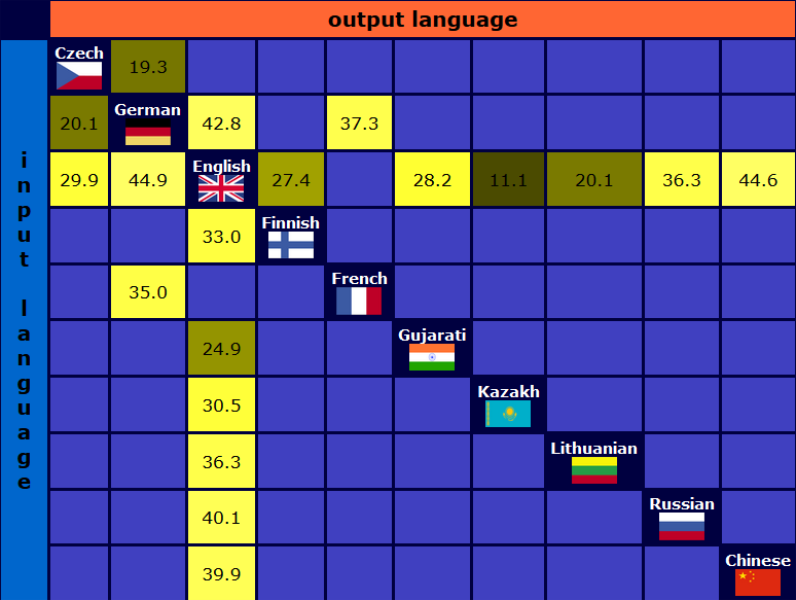
\includegraphics[scale=0.3]{./Chapter1/Figures/figure-wmt-bestresults.jpg}
\setlength{\belowcaptionskip}{-1.5em}
    \caption{WMT\ 19国际机器翻译大赛(左:WMT\ 19参赛队伍;右:WMT\ 19各项目的最好分数)}
    \label{fig:1-5}
\end{figure}
%-------------------------------------------

\parinterval 值得一提的是,近些年神经机器翻译的快速发展也得益于产业界的关注。各大互联网企业和机器翻译技术研发机构都对神经机器翻译的模型和实践方法给予了很大贡献。很多企业凭借自身人才和基础设施方面的优势,先后推出了以神经机器翻译为内核的产品及服务,相关技术方法已经在大规模应用中得到验证,大大推动了机器翻译的产业化进程,而且这种趋势在不断加强,机器翻译的前景也更加宽广。

%----------------------------------------------------------------------------------------
%    NEW SECTION
%----------------------------------------------------------------------------------------

\sectionnewpage
\section{机器翻译现状及挑战}
%%%%%%%%%%%%%%%%%%%%%%%%%%%%%%%%%%%%%%%%%%%%%%%%%%%%%%%%%%%%%%%%%%%%%%%%%%%%
\parinterval 机器翻译技术发展到今天已经过无数次迭代,技术范式也经过若干次更替,近些年机器翻译的应用也如雨后春笋相继浮现。今天的机器翻译的质量究竟如何呢?乐观地说,在很多特定的条件下,机器翻译的译文结果是非常不错的,甚至可以接近人工翻译的结果。然而,在开放式翻译任务中,机器翻译的结果还并不完美。更严格来说,机器翻译的质量远没有达到人们所期望的程度。对于有些人提到的“机器翻译将代替人工翻译”也并不是事实。比如,在高精度同声传译任务中,机器翻译仍需要更多打磨;再比如,针对于小说的翻译,机器翻译还无法做到与人工翻译媲美;甚至有人尝试用机器翻译系统翻译中国古代诗词,这里更多的是娱乐的味道。但是毫无疑问的是,机器翻译可以帮助人类,甚至有朝一日可以代替一些低端的人工翻译工作。

\parinterval 图\ref{fig:1-6}展示了机器翻译和人工翻译质量的一个对比结果。在汉语到英语的新闻翻译任务中,如果对译文进行人工评价(五分制),那么机器翻译的译文得分为3.9分,人工译文得分为4.7分(人的翻译也不是完美的)。可见,在这个任务中机器翻译表现不错,但是与人还有一定差距。如果换一种方式评价,把人的译文作为参考答案,用机器翻译的译文与其进行比对(百分制),会发现机器翻译的得分只有47分。当然,这个结果并不是说机器翻译的译文质量很差,它更多的是表明机器翻译系统可以生成一些与人工翻译不同的译文,机器翻译也具有一定的创造性。这也类似于,很多围棋选手都想向AlphaGo学习,因为智能围棋系统也可以走出一些人类从未走过的妙招。

%----------------------------------------------
\begin{figure}[htp]
   \centering

\definecolor{ublue}{rgb}{0.152,0.250,0.545}
\definecolor{ugreen}{rgb}{0,0.5,0}


%%% outline
%-------------------------------------------------------------------------

{
\begin{tikzpicture}
\node [anchor=south west, fill=blue!50, minimum width=1.1cm, minimum height=2.3cm] (mt) at (1,0) {{\color{white} {\small\sffamily\bfseries{机器}}}};
\node [anchor=south west, fill=red!50, minimum width=1.1cm, minimum height=2.7cm] (human) at ([xshift=0.5cm]mt.south east) {{\color{white} {\small\sffamily\bfseries{人}}}};
\node [anchor=south] (mtscore) at (mt.north) {3.9};
\node [anchor=south] (humanscore) at (human.north) {4.7};
\draw [->,thick] ([xshift=-0.5cm]mt.south west) -- ([xshift=0.5cm]human.south east);
\draw [->,thick] ([xshift=-0.5cm]mt.south west) -- ([xshift=-0.5cm,yshift=3.2cm]mt.south west);

\node [anchor=south west, fill=blue!50, minimum width=1.1cm, minimum height=1.5cm] (mt1) at ([xshift=13.0em,yshift=-3.0em]mt.east) {{\color{white} {\small\sffamily\bfseries{机器}}}};
\node [anchor=south west, fill=red!50, minimum width=1.1cm, minimum height=2.7cm] (human1) at ([xshift=0.5cm]mt1.south east) {{\color{white} {\small\sffamily\bfseries{人}}}};
\node [anchor=south] (mtscore1) at (mt1.north) {47};
\node [anchor=south] (humanscore1) at (human1.north) {100};
\draw [->,thick] ([xshift=-0.5cm]mt1.south west) -- ([xshift=0.5cm]human1.south east);
\draw [->,thick] ([xshift=-0.5cm]mt1.south west) -- ([xshift=-0.5cm,yshift=3.2cm]mt1.south west);

\node[anchor=south](footname1) at ([xshift=2.1em,yshift=-2.0em]mt.south){\footnotesize{人工评价(五分制)}};
\node[anchor=south](footname2) at ([xshift=2.1em,yshift=-2.0em]mt1.south){\footnotesize{自动评价(百分制)}};
\end{tikzpicture}

}






%---------------------------------------------------------------------




\setlength{\belowcaptionskip}{-0.5em}
    \caption{机器翻译与人工翻译性能对比(汉英新闻领域翻译)}
    \label{fig:1-6}
\end{figure}
%-------------------------------------------

\parinterval 图\ref{fig:1-7}展示了一个真实的汉语到英语翻译实例。对比发现,机器翻译与人工翻译还是存在差距的,特别是在翻译一些具有感情色彩的词语时,机器翻译的译文缺一些味道。那么,机器翻译一点用都没有吗?显然不是。实际上,如果考虑翻译速度与翻译代价,机器翻译的价值是无可比拟的。还是同一个例子,翻译一篇短文如果人工翻译需要30分钟甚至更长时间,那么机器翻译仅仅需要两秒,换种情况思考,如果有100万篇这样的文档,其人工翻译的成本根本无法想象,消耗的时间更是难以计算,而计算机集群仅仅需要一天,而且只有电力的消耗。

%----------------------------------------------
\begin{figure}[htp]
    \centering
\definecolor{ublue}{rgb}{0.152,0.250,0.545}
\definecolor{ugreen}{rgb}{0,0.5,0}

%%% outline
%-------------------------------------------------------------------------
\begin{tikzpicture}
%第一段----------------------------------------------
%原文-------------
\node [pos=0.4,left,xshift=-0.4em,yshift=2.0em] (original1) {\scriptsize{源\ \ 语\ \ 言:从前有一个小岛,上面住着快乐、悲哀、知识和爱,还有其他各种情感。一天,情感们得知}};
\node [anchor=north west] (original1-1) at ([xshift=3.5em,yshift=0.3em]original1.south west)  {\scriptsize{小岛快要下沉了。于是,大家都准备船只,离开小岛,只有爱决定留下来,她想坚持到最后}};
\node [anchor=north west] (original1-2) at ([yshift=0.3em]original1-1.south west)  {\scriptsize{一刻。过了几天,小岛真的要下沉了,爱想请人帮忙。}};
%机器翻译--------------
\node [anchor=north west] (mt1) at ([xshift=-3.5em,yshift=0.3em]original1-2.south west) {\scriptsize{机器翻译:Once upon a time there was an island {\color{red}\underline{on which}} lived happiness,sorrow,knowledge,love and other}};

\node [anchor=north west] (mt1-1) at ([xshift=3.5em,yshift=0.4em]mt1.south west) {\scriptsize{emotions. One day, {\color{red}\underline{the}} emotions learned that the island was going to sink.As a result,everyone pre}};

\node [anchor=north west] (mt1-2) at ([yshift=0.4em]mt1-1.south west) {\scriptsize{-pared the boat and {\color{red}\underline{left the island.}} Only Love decided to stay.She {\color{red}\underline{ wanted to stick}} to it until the last}};

\node [anchor=north west] (mt1-3) at ([yshift=0.4em]mt1-2.south west) {\scriptsize{moment. After a few days, the island was really going to sink and love {\color{red}\underline{ wanted help.}}}};
%人工翻译---------------
\node [anchor=north west] (ht1) at ([xshift=-3.5em,yshift=0.4em]mt1-3.south west) {\scriptsize{人工翻译:Once upon a time, there was a small island {\color{red}\underline{where}} lived all kinds of emotions like JOY,SADNESS,}};

\node [anchor=north west] (ht1-1) at ([xshift=3.5em,yshift=0.4em]ht1.south west) {\scriptsize{KNOWLEDGE, and LOVE.One day, {\color{red}\underline{these}} emotions found that the island was sinking, so one by}};

\node [anchor=north west] (ht1-2) at ([yshift=0.4em]ht1-1.south west) {\scriptsize{one they prepared the boat and {\color{red}\underline{planned to leave.}} None but LOVE chose to stay there. She {\color{red}\underline{was deter}}}};

\node [anchor=north west] (ht1-3) at ([yshift=0.4em]ht1-2.south west) {\scriptsize{{\color{red}\underline{-mined to}} persist till the last moment.A few days later, almost the whole island sunk into the sea,}};

\node [anchor=north west] (ht1-4) at ([yshift=0.4em]ht1-3.south west) {\scriptsize{and LOVE had to {\color{red}\underline{seek for help.}}}};

\begin{pgfonlayer}{background}
{
\node[rectangle,draw=ublue, inner sep=0mm] [fit =(original1)(ht1)(mt1)(ht1-4)] {};
}
\end{pgfonlayer}


\end{tikzpicture}





    \caption{机器翻译与人工翻译结果对比实例}
    \label{fig:1-7}
\end{figure}
%-------------------------------------------

\parinterval 虽然机器翻译有上述优点,但仍然面临一些挑战:

\begin{itemize}
\vspace{0.5em}
\item {\small\bfnew{自然语言翻译问题的复杂性极高}}。语言是人类进化的最高成就之一,自然语言具有高度的概括性、灵活性、多样性,这些都很难用几个简单的模型和算法进行描述。因此,翻译问题的数学建模和计算机程序实现难度很大。虽然近几年AlphaGo等人工智能系统在围棋等领域取得了令人瞩目的成绩,但是,相比翻译来说,围棋等棋类任务仍然“简单”。正如不同人对同一句话的理解不尽相同,一个句子往往不存在绝对的标准译文,其潜在的译文几乎是不可穷尽的。甚至人类译员在翻译一个句子、一个单词的时候,都要考虑整个篇章的上下文语境。这些难点都不是传统棋类任务所具有的。
\vspace{0.5em}
\item {\small\bfnew{计算机的“理解”与人类的“理解”存在鸿沟}}。人类一直希望把自己翻译时所使用的知识描述出来,并用计算机程序进行实现,例如早期基于规则的机器翻译方法就源自这个思想。但是,经过实践发现,人和计算机在“理解”自然语言上存在着明显差异。首先,人类的语言能力是经过长时间在多种外部环境因素共同作用下形成的,这种能力很难用计算机准确地刻画。况且人类的语言知识本身就很难描述,更不用说让计算机来理解;其次,人和机器翻译系统理解语言的目的不一样。人理解和使用语言是为了进行生活和工作,而机器翻译系统更多的是为了对某些数学上定义的目标函数进行优化。也就是说,机器翻译系统关注的是翻译这个单一目标,而并不是像人一样进行复杂的活动;此外,人和计算机的运行方式有着本质区别。人类语言能力的生物学机理与机器翻译系统所使用的计算模型本质上是不同的,机器翻译系统使用的是其自身能够理解的“知识”,比如,统计学上的词语表示。这种“知识”并不需要人来理解,当然从系统开发的角度,计算机也并不需要理解人是如何思考的。
\vspace{0.5em}
\item {\small\bfnew{单一的方法无法解决多样的翻译问题}}。首先,语种的多样性会导致任意两种语言之间的翻译实际上都是不同的翻译任务。比如,世界上存在的语言多达几千种,如果选择任意两种语言进行互译就会产生上百万种翻译方向。虽然已经有研究者尝试用同一个框架甚至同一个翻译系统进行全语种的翻译,但是这类系统离真正可用还有很远的距离;其次,不同的领域,不同的应用场景对翻译也有不同的需求。比如,文学作品的翻译和新闻的翻译就有不同、口译和笔译也有不同,类似的情况不胜枚举。以上这些都增加了计算机对翻译进行建模的难度;再次,对于机器翻译来说,充足的高质量数据是必要的,但是不同语种、不同领域、不同应用场景所拥有的数据量有明显差异,很多语种甚至几乎没有可用的数据,这时开发机器翻译系统的难度可想而知。值得注意的是,现在的机器翻译还无法像人类一样在学习少量样例的情况下进行举一反三,因此数据稀缺情况下的机器翻译也给研究者带来了很大的挑战。
\vspace{0.5em}
\end{itemize}

\parinterval 显然,实现机器翻译并不简单,甚至有人把机器翻译看作是实现人工智能的终极目标。幸运的是,今天的机器翻译无论从技术方法上还是从应用上都有了巨大的飞跃,很多问题在不断被求解。如果读者看到过十年前机器翻译的结果,再对比今天的结果,一定会感叹翻译质量的今非昔比,很多译文已经非常准确且流畅。从当今机器翻译的前沿技术看,近三十年机器翻译的进步更多得益于基于数据驱动方法和统计建模方法的使用。特别是近些年深度学习等基于表示学习的端到端方法使得机器翻译的水平达到了新高度。因此,本书将会对基于统计建模和深度学习方法的机器翻译模型、方法和系统实现进行全面介绍和分析,希望这些论述可以对相关内容的学习和科研工作提供参考。

%----------------------------------------------------------------------------------------
%    NEW SECTION
%----------------------------------------------------------------------------------------

\sectionnewpage
\section{基于规则的方法}\label{section-1.4}
%%%%%%%%%%%%%%%%%%%%%%%%%%%%%%%%%%%%%%%%%%%%%%%%%%%%%%%%%%%%%%%%%%%%%%%%%%%%
\parinterval 机器翻译技术大体上可以分为三种方法,分别为基于规则的机器翻译、统计机器翻译以及神经机器翻译。第一代机器翻译技术是主要使用基于规则的机器翻译方法,其主要思想是通过形式文法定义的规则引入源语言和目标语中的语言学知识。此类方法在机器翻译技术诞生之初就被人所关注,特别是在上世纪70年代,以基于规则方法为代表的专家系统是人工智能中最具代表性的研究领域。甚至到了统计机器翻译时代,很多系统中也大量地使用了基于规则的翻译知识表达形式。

\parinterval 早期,基于规则的机器翻译大多依赖人工定义及书写的规则。主要有两类方法\upcite{nirenburg1989knowledge,hutchins1986machine,zarechnak1979history}:一类是基于转换规则的机器翻译方法,简称转换法。另一类是基于中间语言的方法。它们都以词典和人工书写的规则库作为翻译知识,用一系列规则的组合完成翻译。

%----------------------------------------------------------------------------------------
%    NEW SUB-SECTION
%----------------------------------------------------------------------------------------

\subsection{规则的定义}

\parinterval 规则就像语言中的“If-then”语句,如果满足条件,则执行相应的语义动作。比如,可以将待翻译句子中的某个词,使用目标语言单词进行替换,但是这种替换并非随意的,而是在语言学知识的指导下进行的。

\parinterval 图\ref{fig:1-8}展示了一个使用转换法进行翻译的实例。这里,利用一个简单的汉译英规则库完成对句子“我对你感到满意”的翻译。当翻译“我”时,从规则库中找到规则1,该规则表示遇到单词“我”就翻译为“I”;类似地,也可以从规则库中找到规则4,该规则表示翻译调序,即将单词“you”放到“be satisfied with”后面。这种通过规则表示单词之间的对应关系也为统计机器翻译方法提供了思路。如统计机器翻译中,基于短语的翻译模型使用短语对对原文进行替换,详细描述可以参考{\chapterseven}。

%----------------------------------------------
\begin{figure}[htp]
    \centering
\definecolor{ublue}{rgb}{0.152,0.250,0.545}
\definecolor{ugreen}{rgb}{0,0.5,0}


%%% outline
%-------------------------------------------------------------------------

\begin{tikzpicture}
\begin{scope}
{
{\footnotesize
\node [anchor=north west] (rule1) at (0,0) {\textbf{1: If} 源=我, \textbf{then} 译=\ I};
\node [anchor=north west] (rule2) at ([yshift=0.1em]rule1.south west) {\textbf{2: If} 源=你, \textbf{then} 译=\ you};
\node [anchor=north west] (rule3) at ([yshift=0.1em]rule2.south west) {\textbf{3: If} 源=感到\ 满意,};
\node [anchor=north west] (rule3part2) at ([yshift=0.5em]rule3.south west) {\textbf{\hspace{0.95em} then} 译=\ be satisfied with};
\node [anchor=north west] (rule4) at ([yshift=0.1em]rule3part2.south west) {\textbf{4: If} 源=对 ... 动词[表态度]};
\node [anchor=north west] (rule4part2) at ([yshift=0.5em]rule4.south west) {\textbf{\hspace{0.95em} then} 调序[动词 + 对象]};
\node [anchor=north west] (rule5) at ([yshift=0.1em]rule4part2.south west) {\textbf{5: If} 译文主语是\ I};
\node [anchor=north west] (rule5part2) at ([yshift=0.5em]rule5.south west) {\textbf{\hspace{0.95em} then} be动词为\ am/was};
\node [anchor=north west] (rule6) at ([yshift=0.1em]rule5part2.south west) {\textbf{6: If} 源语是主谓结构};
\node [anchor=north west] (rule6part2) at ([yshift=0.5em]rule6.south west) {\textbf{\hspace{0.95em} then} 译文为主谓结构};
\node [anchor=south west] (rulebaselabel) at (rule1.north west) {{\color{ublue} 资源:规则库}};
}

\begin{pgfonlayer}{background}
{
  \node[rectangle,draw=ublue, thick,inner sep=0mm] [fit = (rule1) (rule2) (rule3) (rule3part2) (rule4) (rule4part2) (rule5) (rule5part2) (rule6) (rule6part2) (rulebaselabel)] {};
}
\end{pgfonlayer}
}

\end{scope}

\begin{scope}[xshift=2.3in]
{\footnotesize
\node [anchor=north west,inner sep=1mm] (w1) at (0,0em) {我};
\node [anchor=north west,inner sep=1mm] (w2) at ([xshift=0.3em]w1.north east) {对};
\node [anchor=north west,inner sep=1mm] (w3) at ([xshift=0.3em]w2.north east) {你};
\node [anchor=north west,inner sep=1mm] (w4) at ([xshift=0.3em]w3.north east) {感到};
\node [anchor=north west,inner sep=1mm] (w5) at ([xshift=0.3em]w4.north east) {满意};
}
\end{scope}

{\footnotesize
\node [anchor=north,inner sep=1mm] (t1) at ([yshift=-0.6em]w1.south) {I};
\draw[->,thick,ublue] (w1.south)--(t1.north);
}

{\footnotesize
\node [anchor=north,inner sep=1mm] (t3) at ([yshift=-0.6em]w3.south) {you};
\draw[->,thick,ublue] (w3.south)--(t3.north);
}

{\footnotesize
\draw[-] ([yshift=0.2em]w4.south west)--([yshift=0.2em]w5.south east);
\node [anchor=north,inner sep=1mm] (t45) at ([yshift=-2em]w5.south) {be satisfied with};
\draw[->,thick,ublue] ([yshift=0.1em]w4.south east)..controls +(south:0.6) and +(north:0.6)..(t45.north);
}

{\footnotesize
\node [anchor=north west,inner sep=1mm] (t35) at ([yshift=-3.0em,xshift=-1em]t3.south) {be satisfied with you};
\draw[->,thick,ublue] (t3.south)..controls +(south:1.3) and +(north:0.9)..([xshift=-1em,yshift=-0.2em]t35.north east);
\draw[->,thick,ublue] (t45.south)..controls +(south:0.7) and +(north:0.5)..([xshift=3em,yshift=-0.2em]t35.north west);
}

{\footnotesize
\node [anchor=north west,inner sep=1mm] (t15) at ([yshift=-1.5em,xshift=-2em]t35.south west) {I be satisfied with you};
\draw[->,thick,ublue] (t35.south)..controls +(south:0.5) and +(north:0.5)..([xshift=-5em]t15.north east);
\draw[->,thick,ublue] (t1.south)..controls +(south:1.5) and +(north:1.5)..([xshift=0.5em]t15.north west);
}


{\footnotesize
\node [anchor=north west,inner sep=1mm] (t15final) at ([yshift=-1.5em]t15.south west) {I am satisfied with you};
\node [draw,circle,thick,dotted,ublue,minimum width=1.3em] (be1) at ([xshift=1.35em,yshift=0.1em]t15.west) {};
\draw[->,thick,ublue] ([xshift=-0em]be1.south)..controls +(south:0.3) and +(north:0.4)..([xshift=1.6em,yshift=-0.2em]t15final.north west);
}
{
\draw[->,dotted,thick,red] ([xshift=-0.2em]rule5part2.east)..controls +(east:1.5) and +( west:1.5)..(t15final.west) node[pos=0.9,below,xshift=0.3em,yshift=0.0em] (applyr6) {\color{red}{\tiny\sffamily\bfseries{规则5}}};
}

\end{tikzpicture}
%---------------------------------------------------------------------



    \caption{基于规则的机器翻译的示例图(左:规则库;右:规则匹配结果)}
    \label{fig:1-8}
\end{figure}
%-------------------------------------------

\parinterval 在上述例子中可以发现,规则不仅仅可以翻译句子之间单词的对应,如规则1,还可以表示句法甚至语法之间的对应,如规则6。因此基于规则的方法可以分成多个层次,如图\ref{fig:1-9}所示。图中不同的层次表示采用不同的知识来书写规则,进而完成机器翻译过程。对于翻译问题,可以构建不同层次的基于规则的机器翻译系统。这里包括四个层次,分别为:词汇转换、句法转换、语义转换和中间语言层。其中,上层可以继承下层的翻译知识,比如说句法转换层会利用词汇转换层知识。早期基于规则的方法属于词汇转换层。

%----------------------------------------------
\begin{figure}[htp]
    \centering
%%%------------------------------------------------------------------------------------------------------------
%%%  短语系统的架构
\begin{center}
\begin{tikzpicture}
\begin{scope}

\tikzstyle{node1} = [minimum width=7em,minimum height=1.7em,fill=red!20,rounded corners=0.3em];
\tikzstyle{node2} = [minimum width=7em,minimum height=2.5em,fill=blue!20,rounded corners=0.3em];
\tikzstyle{node3} = [minimum width=7em,minimum height=2.5em,fill=green!20,rounded corners=0.3em];
\tikzstyle{node4} = [minimum width=7em,minimum height=1.7em,fill=orange!20,rounded corners=0.3em];
\tikzstyle{node5} = [minimum width=4.5em,minimum height=1.7em,dashed];

\node [node1,anchor=south west] (s1) at (0,0) {{ \small{源语言词串}}};
\node [node2,anchor=south] (s2) at ([xshift=2.5em,yshift=2em]s1.north) {};
\node [anchor=north,minimum height=1.2em] (s21) at (s2.north) {{ \small{源语言}}};
\node [anchor=south,minimum height=1.2em] (s22) at (s2.south) {{ \small{句法结构}}};
\node [node3,anchor=south] (s3) at ([xshift=2.5em,yshift=2em]s2.north) {};
\node [anchor=north,minimum height=1.2em] (s31) at (s3.north) {{ \small{源语言}}};
\node [anchor=south,minimum height=1.2em] (s32) at (s3.south) {{ \small{语义结构}}};
\node [node4,anchor=south] (s4) at ([xshift=6em,yshift=2em]s3.north) {{ \small{中间语言(知识表示)}}};

\node [node3,anchor=north] (t1) at ([xshift=6em,yshift=-2em]s4.south) {};
\node [anchor=north,minimum height=1.2em] (t11) at (t1.north) {{ \small{目标语言}}};
\node [anchor=south,minimum height=1.2em] (t12) at (t1.south) {{ \small{语义结构}}};
\node [node2,anchor=north] (t2) at ([xshift=2.5em,yshift=-2em]t1.south) {};
\node [anchor=north,minimum height=1.2em] (t21) at (t2.north) {{ \small{目标语言}}};
\node [anchor=south,minimum height=1.2em] (t22) at (t2.south) {{ \small{句法结构}}};
\node [node1,anchor=north] (t3) at ([xshift=2.5em,yshift=-2em]t2.south) {{ \small{目标语言词串}}};

\node [anchor=north] (l1) at ([yshift=-2em]s4.south) {{ \small{语义\ 转换}}};
\node [anchor=north] (l2) at ([yshift=-3em]l1.south) {{ \small{句法\ 转换}}};
\node [anchor=north] (l3) at ([yshift=-2.5em]l2.south) {{ \small{词汇\ 转换}}};

\node [node5,anchor=north,draw] (st1) at ([xshift=-3em,yshift=-0.5em]l3.south) {{ \small{分析部分}}};
\node [node5,anchor=north,draw] (st2) at ([xshift=3em,yshift=-0.5em]l3.south) {{ \small{生成部分}}};

\draw [->,thick] (s1.north) -- ([xshift=-0.6em]s2.south);
\draw [->,thick] ([xshift=0.6em]s2.north) -- (s3.south);
\draw [->,thick] ([xshift=1.2em]s3.north) -- ([xshift=-2.7em]s4.south);
\draw [->,thick] ([xshift=2.7em]s4.south) -- ([xshift=-1.2em]t1.north);
\draw [->,thick] (t1.south) -- ([xshift=-0.6em]t2.north);
\draw [->,thick] ([xshift=0.6em]t2.south) -- (t3.north);
\draw [->,thick] (s3.east) -- (t1.west);
\draw [->,thick] (s2.east) -- (t2.west);
\draw [->,thick] (s1.east) -- (t3.west);

\draw [-] ([xshift=0.1em]s4.south) -- ([xshift=0.1em,yshift=-14em]s4.south);


\end{scope}
\end{tikzpicture}
\end{center}
    \caption{基于规则的机器翻译方法的四个层次\upcite{冯志伟2004机器翻译研究}}
\setlength{\belowcaptionskip}{-1.5em}
    \label{fig:1-9}
\end{figure}
%-------------------------------------------

%----------------------------------------------------------------------------------------
%    NEW SUB-SECTION
%----------------------------------------------------------------------------------------

\subsection{转换法}

\parinterval 通常一个典型的{\small\bfnew{基于转换规则的机器翻译}}\index{基于转换规则的机器翻译}(Transfer-based Translation)\index{Transfer-based Translation}的过程可以被视为“独立分析-相关转换-独立生成”的过程\upcite{parsing2009speech}。如图\ref{fig:1-10}所示,这些过程可以分成六个步骤,其中每一个步骤都是通过相应的翻译规则来完成。比如,第一个步骤中需要构建源语词法分析规则,第二个步骤中需要构建源语句法分析规则,第三个和第四个步骤中需要构建转换规则,其中包括源语言-目标语言词汇和结构转换规则等等。

%----------------------------------------------
\begin{figure}[htp]
    \centering
%%%------------------------------------------------------------------------------------------------------------
%%%  短语系统的架构
\begin{center}
\begin{tikzpicture}
\begin{scope}

\tikzstyle{datanode} = [minimum width=7em,minimum height=1.7em,fill=red!20,rounded corners=0.3em];
\tikzstyle{modelnode} = [minimum width=7em,minimum height=1.7em,fill=blue!20,rounded corners=0.3em];
\tikzstyle{decodingnode} = [minimum width=7em,minimum height=1.7em,fill=green!20,rounded corners=0.3em];

\node [datanode,anchor=north west,minimum height=1.7em,minimum width=8em] (s1) at (0,0) {{ \small{源文句子}}};
\node [modelnode,anchor=north,minimum height=1.7em,minimum width=8em] (s2) at ([yshift=-1.5em]s1.south) {{ \small{源语词法分析}}};
\node [datanode,anchor=north,minimum height=1.7em,minimum width=8em] (s3) at ([yshift=-1.5em]s2.south) {{ \small{源文词串}}};
\node [modelnode,anchor=north,minimum height=1.7em,minimum width=8em] (s4) at ([yshift=-1.5em]s3.south) {{ \small{源语句法分析}}};
\node [datanode,anchor=north,minimum height=1.7em,minimum width=8em] (s5) at ([yshift=-1.5em]s4.south) {{ \small{源文结构}}};

\node [datanode,anchor=west,minimum height=1.7em,minimum width=8em] (t1) at ([xshift=14em]s1.east) {{ \small{译文句子}}};
\node [modelnode,anchor=north,minimum height=1.7em,minimum width=8em] (t2) at ([yshift=-1.5em]t1.south) {{ \small{目标语词法生成}}};
\node [datanode,anchor=north,minimum height=1.7em,minimum width=8em] (t3) at ([yshift=-1.5em]t2.south) {{ \small{译文词串}}};
\node [modelnode,anchor=north,minimum height=1.7em,minimum width=8em] (t4) at ([yshift=-1.5em]t3.south) {{ \small{目标语句法生成}}};
\node [datanode,anchor=north,minimum height=1.7em,minimum width=8em] (t5) at ([yshift=-1.5em]t4.south) {{ \small{译文结构}}};

\node [decodingnode,anchor=west,minimum height=1.7em,minimum width=8em] (st1) at ([xshift=2.5em,yshift=0.85em]s5.east) {{ \small{源语-目标语词汇转换}}};
\node [decodingnode,anchor=north,minimum height=1.7em,minimum width=8em] (st2) at ([yshift=0.05em]st1.south) {{ \small{源语-目标语结构转换}}};

\draw [->,very thick] (s1.south) -- (s2.north);
\draw [->,very thick] (s2.south) -- (s3.north);
\draw [->,very thick] (s3.south) -- (s4.north);
\draw [->,very thick] (s4.south) -- (s5.north);
\draw [->,very thick] (s5.east) -- (st1.south west);
\draw [->,very thick] (st1.south east) -- (t5.west);
\draw [->,very thick] (t5.north) -- (t4.south);
\draw [->,very thick] (t4.north) -- (t3.south);
\draw [->,very thick] (t3.north) -- (t2.south);
\draw [->,very thick] (t2.north) -- (t1.south);

\end{scope}
\end{tikzpicture}
\end{center}
    \caption{基于转换规则的机器翻译过程}
    \label{fig:1-10}
\end{figure}
%-------------------------------------------

\parinterval 转换法的目标就是使用规则定义的词法和句法,将源语言句子分解成为一个蕴含语言学标志的结构。如一个汉语句子“她把一束花放在桌上。”,经过词法和句法分析之后可以被表示成如图\ref{fig:1-11} 所示的结构,这个结构就是图\ref{fig:1-10}中的源语言句子结构。这种使用语言学提取句子结构化表示,并使用某种规则匹配源语言结构和目标语言结构的方式也为{\chaptereight}将要介绍的基于语言学句法的模型提供了思路。

%----------------------------------------------
\begin{figure}[htp]
    \centering
%------------------------------------------------------------------------------------------------------------
%%%  句法树(层次短语)
\begin{tikzpicture}
{\small
\begin{scope}[sibling distance=25pt, level distance = 20pt]
{\scriptsize
\Tree[.\node(r){IP};
        [.\node(n11){NP}; [.\node(n21){PN};  [.\node(l1){她};]]]
        [.\node(n12){VP}; 
            [.\node(n22){BA}; \node(l2){把}; ]
            [.\node(n23){IP};
                [. \node(n31){NP}; 
                    [. \node(n41){QP}; 
                        [. \node(n51){CD};  \node(l3){一};]
                        [. \node(n52){CLP};  [.\node(n61){M};  [.\node(l4){束};]]]
                    ]
                    [. \node(n42){NP};  [.\node(n53){NN};  [.\node(l5){花};]]]
                ]
                [. \node(n32){VP}; 
                    [. \node(n43){VV};  \node(l6){放在};]
                    [. \node(n44){LCP};
                        [. \node(n54){NP};  [.\node(n62){NN};  [.\node(l7){桌};]]] 
                        [. \node(n55){LC};  \node(l8){上};]
                    ]
                ]
            ]
        ]
        [.\node(n13){PU};  \node(l9){。};]
     ]
}
\end{scope}
}
\end{tikzpicture}

    \caption{一个汉语句子的结构表示(句法树)}
    \label{fig:1-11}
\end{figure}
%-------------------------------------------

\parinterval 在转换法中,翻译规则通常会分成两类:通用规则和个性规则。所谓通用的规则主要用于句法分析、语义分析、结构转换和句法生成等,是不具体依赖于某个源语言或者目标语言词汇而设计的翻译规则;个性规则通常以具体源语言词汇来做索引,比如图\ref{fig:1-8}中规则5就是针对主语是“I”的个性规则,它直接针对某个具体词汇进行分析和翻译。

%----------------------------------------------------------------------------------------
%    NEW SUB-SECTION
%----------------------------------------------------------------------------------------

\subsection{基于中间语言的方法}

\parinterval 基于转换的方法可以通过词汇层、句法层和语义层完成从源语到目标语的转换过程,虽然采用了独立分析和独立生成两个子过程,但中间包含一个从源语到目标语的相关转换过程。这就会导致一个实际问题,假设需要实现$N$个语言之间互译的机器翻译系统,采用基于转换的方法,需要构建$N(N-1)$个不同的机器翻译系统,这个构建代价是非常高的。为了解决这个问题,一种有效的解决方案是使用{\small\bfnew{基于中间语言的机器翻译}}\index{基于中间语言的机器翻译}(Interlingua-based Translation)\index{Interlingua-based Translation}方法。

\parinterval 如图\ref{fig:1-12}所示,基于中间语言方法的最大特点就是采用了一个称之为“中间语言”的知识表示结构,将“中间语言”作为独立源语言分析和独立目标语生成的桥梁,真正实现独立分析和独立生成。并且在基于中间语言的方法中不涉及“相关转换”这个过程,这一点与基于转换的方法有很大区别。

%----------------------------------------------
\begin{figure}[htp]
    \centering
%%%------------------------------------------------------------------------------------------------------------
%%%  短语系统的架构
\begin{center}
\begin{tikzpicture}
\begin{scope}

\tikzstyle{datanode} = [minimum width=5em,minimum height=1.7em,fill=red!20,rounded corners=0.3em];
\tikzstyle{modelnode} = [minimum width=5em,minimum height=1.7em,fill=blue!20,rounded corners=0.3em];
\tikzstyle{decodingnode} = [minimum width=5em,minimum height=1.7em,fill=green!20,rounded corners=0.3em];

\node [datanode,anchor=north west] (s1) at (0,0) {{ \small{语言1}}};
\node [datanode,anchor=north] (s2) at ([yshift=-4.5em]s1.south) {{ \small{语言3}}};
\node [datanode,anchor=west] (s3) at ([xshift=4.5em]s1.east) {{ \small{语言2}}};
\node [datanode,anchor=north] (s4) at ([yshift=-4.5em]s3.south) {{ \small{语言4}}};
\node [circle,anchor=north west,inner sep=2pt,fill=blue!20] (m1) at ([xshift=0.8em,yshift=-0.5em]s1.south east) {{ \small{中间语言}}};

\draw [<->,very thick] (s1.south) -- (m1.170);
\draw [<->,very thick] (s2.north) -- (m1.190);
\draw [<->,very thick] (s3.south) -- (m1.10);
\draw [<->,very thick] (s4.north) -- (m1.-10);

\node [anchor=north] (l) at ([xshift=5em,yshift=-1em]s2.south) {\footnotesize{(a) 基于中间语言的方法}};


\end{scope}

\begin{scope}[xshift=16em]

\tikzstyle{datanode} = [minimum width=5em,minimum height=1.7em,fill=red!20,rounded corners=0.3em];
\tikzstyle{modelnode} = [minimum width=5em,minimum height=1.7em,fill=blue!20,rounded corners=0.3em];
\tikzstyle{decodingnode} = [minimum width=5em,minimum height=1.7em,fill=green!20,rounded corners=0.3em];

\node [datanode,anchor=north west] (s1) at (0,0) {{ \small{语言1}}};
\node [datanode,anchor=north] (s2) at ([yshift=-4.5em]s1.south) {{ \small{语言3}}};
\node [datanode,anchor=west] (s3) at ([xshift=4.5em]s1.east) {{ \small{语言2}}};
\node [datanode,anchor=north] (s4) at ([yshift=-4.5em]s3.south) {{ \small{语言4}}};

\draw [<->,very thick] (s1.south) -- (s2.north);
\draw [<->,very thick] (s1.east) -- (s3.west);
\draw [<->,very thick] (s3.south) -- (s4.north);
\draw [<->,very thick] (s2.east) -- (s4.west);
\draw [<->,very thick] (s1.south east) -- (s4.north west);
\draw [<->,very thick] (s2.north east) -- (s3.south west);

\node [anchor=north] (l) at ([xshift=5em,yshift=-1em]s2.south) {\footnotesize{(b) 基于转换的方法}};

\end{scope}

\end{tikzpicture}
\end{center}
    \caption{基于中间语言的方法(a)与基于转换的方法(b)}
    \label{fig:1-12}
\end{figure}
%-------------------------------------------

\parinterval 从图\ref{fig:1-9}可以发现,中间语言(知识表示)处于最顶端,本质上是独立于源语言和目标语言的,这也是基于中间语言的方法可以将分析过程和生成过程分开的原因。

\parinterval 虽然基于中间语言的方法有上述优点,但如何定义中间语言是一个关键问题。严格上说,所谓中间语言本身是一种知识表示结构,承载着源语言句子的分析结果,应该包含和体现尽可能多的源语言知识。如果中间语言的表示能力不强,会导致源语言句子信息丢失,这自然会影响目标语生成结果。

\parinterval 在基于规则的机器翻译方法中,构建中间语言结构的知识表示方式有很多,比较常见的是语法树、语义网、逻辑结构表示或者多种结构的融合等。但不管哪种方法,实际上都无法充分地表达源语言句子所携带的信息。因此,在早期的基于规则的机器翻译研究中,基于中间语言的方法明显弱于基于转换的机器翻译方法。不过,近些年随着神经机器翻译等方法的兴起,使用统一的中间表示来刻画句子又受到了广泛关注。但是,神经机器翻译中的“中间表示”并不是规则系统中的中间语言,二者有着本质区别,这部分内容将会在第十章进行介绍。

%----------------------------------------------------------------------------------------
%    NEW SUB-SECTION
%----------------------------------------------------------------------------------------

\subsection{规则方法的优缺点}

\parinterval 在基于规则的机器翻译时代,机器翻译技术研究有一个特点就是{\small\bfnew{语法}}\index{语法}(Grammer)\index{Grammer}和{\small\bfnew{算法}}\index{算法}(Algorithm)\index{Algorithm}分开,相当于是把语言分析和程序设计分开。传统方式使用程序代码来实现翻译规则,并把所谓的翻译规则隐含在程序代码实现中。其中最大问题是一旦翻译规则发生修改,程序代码也需要进行相应修改,导致维护代价非常高。此外书写翻译规则的语言学家与编代码的程序员沟通代价也非常高,有时候会出现鸡同鸭讲的感觉。把语法和算法分开对于基于规则的机器翻译技术来说最大好处就是可以将语言学家和程序员的工作分开,各自发挥自己的优势。

\parinterval 这种语言分析和程序设计分开的实现方式也使得基于人工书写翻译规则的机器翻译方法非常直观,语言学家可以很容易地将翻译知识利用规则的方法表达出来,并且不需要修改系统代码。例如:1991年,东北大学自然语言处理实验室王宝库教授提出的规则描述语言(CTRDL)\upcite{王宝库1991机器翻译系统中一种规则描述语言}。以及1995年,同为东北大学自然语言处理实验室的姚天顺教授提出的词汇语义驱动算法\upcite{唐泓英1995基于搭配词典的词汇语义驱动算法},都是在这种思想上对机器翻译方法的一种改进。此外,使用规则本身就具有一定的优势:

\begin{itemize}
\vspace{0.5em}
\item 翻译规则的书写颗粒度具有很大的可伸缩性。
\vspace{0.5em}
\item 较大颗粒度的翻译规则有很强的概括能力,较小颗粒度的翻译规则具有精细的描述能力。
\vspace{0.5em}
\item 翻译规则便于处理复杂的句法结构和进行深层次的语义理解,比如解决翻译过程中的长距离依赖问题。
\vspace{0.5em}
\end{itemize}

\parinterval 通过图\ref{fig:1-8}中规则的翻译实例中可以看出,规则的使用和人类进行翻译时所使用的思想非常类似,可以说基于规则的方法实际上在试图描述人类进行翻译的思维过程。虽然直接模仿人类的翻译方式对翻译问题建模是合理的,但是这一定程度上也暴露了基于规则的方法的弱点。基于规则的机器翻译方法中,人工书写翻译规则的主观因素重,有时与客观事实有一定差距。并且人工书写翻译规则的难度大,代价非常高,这也成为了后来基于数据驱动的机器翻译方法主要改进的方向。

%----------------------------------------------------------------------------------------
%    NEW SECTION
%----------------------------------------------------------------------------------------

\sectionnewpage
\section{数据驱动的方法}
%%%%%%%%%%%%%%%%%%%%%%%%%%%%%%%%%%%%%%%%%%%%%%%%%%%%%%%%%%%%%%%%%%%%%%%%%%%%
\parinterval 虽然基于规则的方法有种种优势,但是该方法人工代价过高。所以研究者们开始尝试,是否可以更好地利用数据,从数据中学习到某些规律,而不是完全依靠人类来制定规则。在这样的思想下,基于数据驱动的方法诞生了。

%----------------------------------------------------------------------------------------
%    NEW SUB-SECTION
%----------------------------------------------------------------------------------------

\subsection{基于实例的机器翻译}

\parinterval 在实际使用上,\ref{section-1.4}章提到的基于规则的方法更多地被使用在受限翻译场景中,比如受限词汇集的翻译。针对基于规则的方法存在的问题,基于实例的机器翻译于上世纪80年代中期被提出\upcite{nagao1984framework}。该方法的基本思想是在双语句库中找到与待翻译句子相似的实例,之后对实例的译文进行修改,如对译文进行替换、增加、删除等一系列操作,从而得到最终译文。这个过程可以类比人类学习并运用语言的过程:人会先学习一些翻译实例或者模板,当遇到新的句子时,会用以前的实例和模板作对比,之后得到新的句子的翻译结果。这也是一种举一反三的思想。

\parinterval 图\ref{fig:1-13}展示了一个基于实例的机器翻译过程。它利用简单的翻译实例库与翻译词典完成对句子“我对你感到满意”的翻译。首先,使用待翻译句子的源语言端在翻译实例库中进行比较,根据相似度大小找到相似的实例“我对他感到高兴”。然后,标记实例中不匹配的部分,即“你”和“他”,“满意”和“高兴”。再查询翻译词典得到词“你”和“满意”所对应的翻译结果“you”和“satisfied”,用这两个词分别替换实例中的“him”和“happy”,从而得到最终译文。

%----------------------------------------------
\begin{figure}[htp]
    \centering

\definecolor{ublue}{rgb}{0.152,0.250,0.545}
\definecolor{ugreen}{rgb}{0,0.5,0}


%%% outline
%-------------------------------------------------------------------------

\begin{tikzpicture}
\begin{scope}
{
{\footnotesize
\node [anchor=north west] (example1) at (0,0) {\textbf{1:} 源=什么\ 时候\ 开始};
\node [anchor=north west] (example1part2) at ([yshift=0.5em]example1.south west) {\hspace{1em} 译=\ When will it start};
\node [anchor=north west] (example2) at ([yshift=0.1em]example1part2.south west) {\textbf{2:} 源=我\ 对\ 他\ 感到\ 高兴};
\node [anchor=north west] (example2part2) at ([yshift=0.5em]example2.south west) {\hspace{1em} 译=\ I am happy with him};
\node [anchor=north west] (example3) at ([yshift=0.1em]example2part2.south west) {\hspace{1em} ...};
\node [anchor=south west] (examplebaselabel) at (example1.north west) {{\color{ublue} 资源1:翻译实例库}};
}
}

\begin{pgfonlayer}{background}
{
\node[rectangle,draw=ublue, inner sep=0mm] [fit = (example1) (example1part2) (example2) (example2part2) (example3) (examplebaselabel)] {};
}
\end{pgfonlayer}

\end{scope}

\begin{scope} [yshift=-1.3in]
{\footnotesize
{
\node [anchor=north west] (entry1) at (0,0) {\textbf{1:} 我 $\to$ I $\mid$ me};
\node [anchor=north west] (entry2) at ([yshift=0.1em]entry1.south west) {\textbf{2:} 你 $\to$ you};
\node [anchor=north west] (entry3) at ([yshift=0.1em]entry2.south west) {\textbf{3:} 满意 \hspace{-0.4em} $\to$ \hspace{-0.4em} satisfy \hspace{-0.12em}$\mid$\hspace{-0.12em} satisfied ... };
\node [anchor=north west] (entry4) at ([yshift=0.1em]entry3.south west) {\hspace{1em} ...};
\node [anchor=south west] (dictionarylabel) at (entry1.north west) {{\color{ublue} 资源2:翻译词典}};
}
}

\begin{pgfonlayer}{background}
{
\node[rectangle,draw=ublue, inner sep=0mm] [fit = (entry1) (entry2) (entry3) (entry4) (dictionarylabel)] {};
}
\end{pgfonlayer}

\end{scope}

\begin{scope}[xshift=2.3in]
{\footnotesize
\node [anchor=north west,inner sep=1mm] (w1) at (0,1.7em) {我};
\node [anchor=north west,inner sep=1mm] (w2) at ([xshift=0.3em]w1.north east) {对};
\node [anchor=north west,inner sep=1mm] (w3) at ([xshift=0.3em]w2.north east) {你};
\node [anchor=north west,inner sep=1mm] (w4) at ([xshift=0.3em]w3.north east) {感到};
\node [anchor=north west,inner sep=1mm] (w5) at ([xshift=0.3em]w4.north east) {满意};
}
\end{scope}

\begin{scope}[xshift=2.3in,yshift=-0.2in]
{\footnotesize
\node [anchor=north west,inner sep=1mm] (c1) at (0,0) {我};
\node [anchor=north west,inner sep=1mm] (c2) at ([xshift=0.3em]c1.north east) {对};
\node [anchor=north west,inner sep=1mm] (c3) at ([xshift=0.3em]c2.north east) {他};
\node [anchor=north west,inner sep=1mm] (c4) at ([xshift=0.3em]c3.north east) {感到};
\node [anchor=north west,inner sep=1mm] (c5) at ([xshift=0.3em]c4.north east) {高兴};
}
\end{scope}

\begin{scope}[xshift=2.3in,yshift=-0.6in]
{\footnotesize
\node [anchor=west,inner sep=1mm] (e1) at (0,0) {I};
\node [anchor=west,inner sep=1mm] (e2) at ([xshift=0.3em]e1.east) {am};
\node [anchor=west,inner sep=1mm] (e3) at ([xshift=0.3em]e2.east) {happy};
\node [anchor=west,inner sep=1mm] (e4) at ([xshift=0.3em]e3.east) {with};
\node [anchor=west,inner sep=1mm] (e5) at ([xshift=0.3em]e4.east) {him};
}
\end{scope}

{
\draw[<->,dotted,thick,red] (example2.east)..controls +(east:0.6) and +(west:0.6)..(c1.west) node[pos=0.9,left,xshift=0.6em,yshift=0.4em] (simexample) {\color{red}{\tiny{相似实例}}};
\draw[<->,dotted,thick,red] ([xshift=-0.2em]example2part2.east)..controls +(east:0.5) and +(west:0.5)..(e1.west);
}

{
\draw[<->,dotted,thick,ublue] (w3.south)--(c3.north) node[pos=0.5,right] (mismatch1) {\color{red}{\tiny{不匹配}}};
\draw[dotted,thick,ublue] ([xshift=-0.6em,yshift=0.0em]c3.south east)--([xshift=0.8em,yshift=0.0em]e5.north west);
}

{
\draw[<->,dotted,thick,ublue] (w5.south)--(c5.north) node[pos=0.5,right] (mismatch1) {\color{red}{\tiny{不匹配}}};
\draw[dotted,thick,ublue] ([xshift=0.8em,yshift=0.0em]c5.south west)--([xshift=0.0em,yshift=-0.2em]e3.north);
}

{
\draw[double,->,thick,ublue] (e3.south)--([yshift=-1.2em]e3.south) node[pos=0.5,right,xshift=0.2em,yshift=0.2em] (step1) {\color{red}{\tiny{用“你”替换“他”}}};

\draw[->,dotted,thick,red] ([xshift=-0.1em]entry2.east)..controls +(east:4) and +(west:4)..([yshift=-0.6em,xshift=-0.5em]e3.south) ;
}

\begin{scope}[xshift=2.3in,yshift=-0.9in]
{\footnotesize
\node [anchor=north west,inner sep=1mm] (c1) at (0,0) {我};
\node [anchor=north west,inner sep=1mm] (c2) at ([xshift=0.3em]c1.north east) {对};
\node [anchor=north west,inner sep=1mm] (c3) at ([xshift=0.3em]c2.north east) {\footnotesize{{\color{ublue} 你}}};
\node [anchor=north west,inner sep=1mm] (c4) at ([xshift=0.3em]c3.north east) {感到};
\node [anchor=north west,inner sep=1mm] (c5) at ([xshift=0.3em]c4.north east) {高兴};
}
\end{scope}

\begin{scope}[xshift=2.3in,yshift=-1.3in]
{\footnotesize
\node [anchor=west,inner sep=1mm] (e1) at (0,0) {I};
\node [anchor=west,inner sep=1mm] (e2) at ([xshift=0.3em]e1.east) {am};
\node [anchor=west,inner sep=1mm] (e3) at ([xshift=0.3em]e2.east) {happy};
\node [anchor=west,inner sep=1mm] (e4) at ([xshift=0.3em]e3.east) {with};
\node [anchor=west,inner sep=1mm] (e5) at ([xshift=0.3em,yshift=-0.2em]e4.east) {\textbf{{\color{ublue} you}}};
}
\end{scope}

{
\draw[dotted,thick,ublue] ([xshift=-0.6em,yshift=0.0em]c3.south east)--([xshift=0.8em,yshift=0.0em]e5.north west);
}

{
\draw[double,->,thick,ublue] (e3.south)--([yshift=-1.2em]e3.south) node[pos=0.5,right,xshift=0.2em,yshift=0.2em] (step1) {\color{red}{\tiny{用“满意”替换“高兴”}}};

\draw[->,dotted,thick,red] ([xshift=-1.2em,yshift=-0.6em]entry3.north east)..controls +(east:2) and +(west:3)..([yshift=-0.6em,xshift=-0.5em]e3.south) ;
}

\begin{scope}[xshift=2.3in,yshift=-1.6in]
{\footnotesize
\node [anchor=north west,inner sep=1mm] (c1) at (0,0) {我};
\node [anchor=north west,inner sep=1mm] (c2) at ([xshift=0.3em]c1.north east) {对};
\node [anchor=north west,inner sep=1mm] (c3) at ([xshift=0.3em]c2.north east) {你};
\node [anchor=north west,inner sep=1mm] (c4) at ([xshift=0.3em]c3.north east) {感到};
\node [anchor=north west,inner sep=1mm] (c5) at ([xshift=0.3em]c4.north east) {\footnotesize{{\color{ublue} 满意}}};
}
\end{scope}

\begin{scope}[xshift=2.3in,yshift=-2.0in]
{\footnotesize
\node [anchor=west,inner sep=1mm] (e1) at (0,0) {I};
\node [anchor=west,inner sep=1mm] (e2) at ([xshift=0.3em]e1.east) {am};
\node [anchor=west,inner sep=1mm] (e3) at ([xshift=0.3em]e2.east) {\textbf{{\color{ublue} satisfied}}};
\node [anchor=west,inner sep=1mm] (e4) at ([xshift=0.3em]e3.east) {with};
\node [anchor=west,inner sep=1mm] (e5) at ([xshift=0.3em,yshift=-0.2em]e4.east) {you};
}
\end{scope}

{
\draw[dotted,thick,ublue] ([xshift=1.0em,yshift=0.0em]c5.south west)--([xshift=0.0em,yshift=-0.2em]e3.north);
}

\begin{pgfonlayer}{background}
{\footnotesize
\node[rectangle,draw=red,thick,inner sep=0mm] [fit = (e1) (e2) (e3) (e4) (e5)] {};
\node[anchor=north] (outputlabel) at (e3.south) {\footnotesize{\color{red}{输出翻译结果}}};
}
\end{pgfonlayer}

\end{tikzpicture}

%---------------------------------------------------------------------




    \caption{基于实例的机器翻译的示例图(左:实例库;右:翻译结果)}
    \label{fig:1-13}
\end{figure}
%-------------------------------------------

\parinterval 当然,基于实例的机器翻译也并不完美:

\begin{itemize}
\vspace{0.5em}
\item 这种方法对翻译实例的精确度要求非常高,一个实例的错误可能会导致一个句型都无法翻译正确。
\vspace{0.5em}
\item 实例维护较为困难,实例库的构建通常需要单词级对齐的标注,而保证词对齐的质量是非常困难的工作,这也大大增加了实例库维护的难度。
\vspace{0.5em}
\item 尽管可以通过实例或者模板进行翻译,但是其覆盖度仍然有限。在实际应用中,很多句子无法找到可以匹配的实例或者模板。
\vspace{0.5em}
\end{itemize}

%----------------------------------------------------------------------------------------
%    NEW SUB-SECTION
%----------------------------------------------------------------------------------------

\subsection{统计机器翻译}

\parinterval 统计机器翻译兴起于上世纪90年代\upcite{brown1990statistical,gale1993a},它利用统计模型从单/双语语料中自动学习翻译知识。具体来说,可以使用单语语料学习语言模型,使用双语平行语料学习翻译模型,并使用这些统计模型完成对翻译过程的建模。整个过程不需要人工编写规则,也不需要从实例中构建翻译模板。无论是词还是短语,甚至是句法结构,统计机器翻译系统都可以自动学习。人更多的是定义翻译所需的特征和基本翻译单元的形式,而翻译知识都保存在模型的参数中。

\parinterval 图\ref{fig:1-14}展示了一个统计机器翻译系统运行的简单实例。整个系统需要两个模型:翻译模型和语言模型。其中,翻译模型从双语平行语料中学习翻译知识,得到短语表,短语表包含了各种词汇的翻译及其概率,这样可以度量源语言和目标语言片段之间互为翻译的可能性大小;语言模型从单语语料中学习目标语的词序列生成规律,来衡量目标语言译文的流畅性。最后,将这两种模型联合使用,通过翻译引擎来搜索尽可能多的翻译结果,并计算不同翻译结果的可能性大小,最后将概率最大的译文作为最终结果输出。这个过程并没有显性地使用人工翻译规则和模板,译文的生成仅仅依赖翻译模型和语言模型中的统计参数。

%----------------------------------------------
\begin{figure}[htp]
    \centering
\definecolor{ublue}{rgb}{0.152,0.250,0.545}
\definecolor{ugreen}{rgb}{0,0.5,0}

%%% outline
%-------------------------------------------------------------------------

\begin{tikzpicture}

{
\begin{scope}
{\scriptsize
\node [anchor=north west] (example1) at (0,0) {\textbf{1:} 源=他\ 在\ 哪};
\node [anchor=north west] (example1part2) at ([yshift=0.2em]example1.south west) {\hspace{1em} 译=\ Where is he};
\node [anchor=north west] (example2) at ([yshift=0.1em]example1part2.south west) {\textbf{2:} 源=我\ 真高兴};
\node [anchor=north west] (example2part2) at ([yshift=0.2em]example2.south west) {\hspace{1em} 译=\ I'm so happy};
\node [anchor=north west] (example3) at ([yshift=0.1em]example2part2.south west) {\textbf{3:} 源=出发};
\node [anchor=north west] (example3part2) at ([yshift=0.2em]example3.south west) {\hspace{1em} 译=\ Let's go};
\node [anchor=north west] (example4) at ([yshift=0.1em]example3part2.south west) {\hspace{1em} ...};
\node [anchor=north west] (example5) at ([yshift=0.1em]example4.south west) {\hspace{1em}\quad};
\node [anchor=north west] (example6) at ([yshift=0.1em]example5.south west) {\hspace{1em}\quad};
\node [anchor=south west] (bidatalabel) at (example1.north west) {{\color{ublue}\small{资源1:双语平行语料}}};
}

\begin{pgfonlayer}{background}
{
\node[rectangle,draw=ublue, inner sep=0mm] [fit = (example1) (example1part2) (example2) (example2part2) (example3) (example3part2) (example4) (bidatalabel)(example6)] (bidata) {};
}
\end{pgfonlayer}

\end{scope}
}

{
\begin{scope} [yshift=-1.55in]
{\scriptsize
\node [anchor=north west] (entry1) at (0,0) {\textbf{1:} What is NiuTrans\qquad \qquad };
\node [anchor=north west] (entry2) at ([yshift=0.0em]entry1.south west) {\textbf{2:} Are you fulfilled};
\node [anchor=north west] (entry3) at ([yshift=0.0em]entry2.south west) {\textbf{3:} You are right};
\node [anchor=north west] (entry4) at ([yshift=0.0em]entry3.south west) {\hspace{1em} ...};
\node [anchor=north west] (entry5) at ([yshift=0.1em]entry4.south west) {\hspace{1em}{\quad}};
\node [anchor=north west] (entry6) at ([xshift=11.6em,yshift=0.65em]entry5.south west) {};
\node [anchor=south west] (monodatalabel) at (entry1.north west) {{\color{ublue}\small{资源2:单语语料}}};
}

\begin{pgfonlayer}{background}
{
\node[rectangle,draw=ublue, inner sep=0mm] [fit = (entry1) (entry2) (entry3) (entry4) (entry5)(entry6)(monodatalabel)] (monodata) {};
}
\end{pgfonlayer}

\end{scope}
}

{
\begin{scope}[xshift=1.7in]
{\scriptsize
\node [anchor=north west] (phrase1) at (0,0) {$\textrm{Pr}(\textrm{我} \to \textrm{I}) = 0.7$};
\node [anchor=north west] (phrase2) at ([yshift=0.1em]phrase1.south west) {$\textrm{Pr}(\textrm{我} \to \textrm{me}) = 0.3$};
\node [anchor=north west] (phrase3) at ([yshift=0.1em]phrase2.south west) {$\textrm{Pr}(\textrm{你} \to \textrm{you}) = 0.9$};
\node [anchor=north west] (phrase4) at ([yshift=0.1em]phrase3.south west) {$\textrm{Pr}(\textrm{开心} \to \textrm{happy})$};
\node [anchor=north west] (phrase4part2) at ([yshift=0.5em]phrase4.south west) {$ = 0.5$};
\node [anchor=north west] (phrase5) at ([yshift=0.1em]phrase4part2.south west) {$\textrm{Pr}(\textrm{满意} \to \textrm{satisfied})$};
\node [anchor=north west] (phrase5part2) at ([yshift=0.5em]phrase5.south west) {$ = 0.4$};
\node [anchor=north west] (phrase6) at ([yshift=0.0em]phrase5part2.south west) {...\vspace{2em}};
\node [anchor=north west] (phrase7) at ([yshift=0.6em]phrase6.south west) {};
\node [anchor=south west] (phrasetablelabel) at (phrase1.north west) {{\color{ublue} \small{翻译模型}}};
}

\begin{pgfonlayer}{background}
{
\node[rectangle,draw=ublue, inner sep=0mm] [fit = (phrase1) (phrase2) (phrase3) (phrase4) (phrase4part2) (phrase5) (phrase5part2) (phrase6)(phrase7) (phrasetablelabel)] (phrasetable) {};
}
\end{pgfonlayer}

\end{scope}
}

{
\begin{scope}[xshift=1.7in,yshift=-1.55in]
{\scriptsize
\node [anchor=north west] (ngram1) at (0,0) {$\textrm{Pr}(\textrm{I}) = 0.0001$};
\node [anchor=north west] (ngram2) at ([yshift=0.0em]ngram1.south west) {$\textrm{Pr}(\textrm{I}\ \textrm{am}) = 0.623$};
\node [anchor=north west] (ngram3) at ([yshift=0.0em]ngram2.south west) {$\textrm{Pr}(\textrm{I}\ \textrm{was}) = 0.21$};
\node [anchor=north west] (ngram4) at ([yshift=-0.2em]ngram3.south west) {...};
\node [anchor=north east] (ngrame) at ([yshift=-1in]phrase5.south east) {};
\node [anchor=south west] (lmlabel) at (ngram1.north west) {{\color{ublue} \small{语言模型}}};
}

\begin{pgfonlayer}{background}
{
\node[rectangle,draw=ublue, inner sep=0mm] [fit = (ngram1) (ngram2) (ngram3) (ngram4) (lmlabel) (ngrame)] (langaugemodel) {};
}
\end{pgfonlayer}

\end{scope}
}

{
\draw[->,thick,ublue] (bidata.east)--([xshift=2.2em]bidata.east) node[pos=0.5,above] (simexample) {\color{red}{\scriptsize{\scriptsize{学习}}}};
}

{
\draw[->,thick,ublue] (monodata.east)--([xshift=2.2em]monodata.east) node[pos=0.5,above] (simexample) {\color{red}{\scriptsize{\scriptsize{学习}}}};
}

\begin{scope}[xshift=3.6in]
{\footnotesize
{
\node[anchor=center] (srcsentence) at (0,0) {我 对 你 感到 满意};
}

{
\node[anchor=north west] (translations) at ([xshift=-1em,yshift=-1em]srcsentence.south west) {
{\scriptsize
\begin{tabular}{l | l}
翻译假设 & {概率} \\
\hline
I to you happy & {0.01}\\
You satisfied & {0.02}\\
I satisfied with you & {0.10}\\
I'm satisfied with you & {0.46}\\
I satisfied you, what & {0.23}\\
You can have it & {0.01}\\
You and me & {0.02}\\
\end{tabular}
}
};
}

{
\node[anchor=west,double,draw=ublue,thick] (decoder) at ([xshift=1em,yshift=-13em]srcsentence.south west) {翻译引擎};

\draw[->,thick,ublue] ([yshift=1em]phrasetable.south east) .. controls +(east:1.0em) and +(west:2.5em) .. (decoder.west);
\draw[->,thick,ublue] ([yshift=-2em]langaugemodel.east) .. controls +(east:1.0em) and +(west:1.5em) .. (decoder.west);
}

{
\draw[->,thick,double,ublue] (decoder.north) -- ([yshift=2.2em]decoder.north) node[pos=0.5,right] (decodinglabel) {\color{red}{\tiny{枚举所有可能}}};
}

{
\draw[->,thick,double,ublue] (decoder.east) .. controls +(east:3.5em) .. ([xshift=3.5em,yshift=3.0em]decoder.east) node[xshift=0.5em,pos=0.3,below] (decodinglabel) {\color{red}{\tiny{计算翻译可能性}}};
}

{
\node[anchor=west,draw,thick,red,minimum width=11.5em,minimum height=1em] (outputlabel) at ([xshift=-0.3em,yshift=-6.1em]srcsentence.south west){};
\node[anchor=west] (outputlabel2) at ([xshift=-0.3em]outputlabel.east) {\color{red}{\tiny{输出}}};
}

}
\end{scope}

\end{tikzpicture}

%---------------------------------------------------------------------



    \caption{统计机器翻译的示例图(左:语料资源;中:翻译模型与语言模型;右:翻译假设与翻译引擎)}
    \label{fig:1-14}
\end{figure}
%-------------------------------------------

\parinterval 由于没有对翻译过程进行过多的限制,统计机器翻译有很灵活的译文生成方式,因此系统可以处理更加多样的句子。但是这种方法也带来了一些问题:首先,虽然并不需要人工定义翻译规则或模板,但统计机器翻译系统仍然需要人工定义翻译特征。提升翻译品质往往需要大量的特征工程,这导致人工特征设计的好坏会对系统产生决定性影响;其次,统计机器翻译的模块较多,系统研发比较复杂;再次,随着训练数据增多,统计机器翻译的模型(比如短语翻译表)会明显增大,对系统存储资源消耗较大。

%----------------------------------------------------------------------------------------
%    NEW SUB-SECTION
%----------------------------------------------------------------------------------------

\subsection{神经机器翻译}

\parinterval 随着机器学习技术的发展,基于深度学习的神经机器翻译逐渐兴起。自2014年开始,它在短短几年内已经在大部分任务上取得了明显的优势\upcite{NIPS2014_5346,bahdanau2014neural,vaswani2017attention,DBLP:journals/corr/GehringAGYD17,DBLP:journals/corr/LuongPM15}。在神经机器翻译中,词串被表示成实数向量,即分布式向量表示。这样,翻译过程并不是在离散化的单词和短语上进行,而是在实数向量空间上计算。因此与之前的技术相比,它在词序列表示的方式上有着本质的改变。通常,机器翻译可以被看作一个序列到另一个序列的转化。在神经机器翻译中,序列到序列的转化过程可以由{\small\bfnew{编码器-解码器}}\index{编码器-解码器}(Encoder-Decoder)\index{Encoder-Decoder}框架实现。其中,编码器把源语言序列进行编码,并提取源语言中的信息进行分布式表示,之后解码器再把这种信息转换为另一种语言的表达。

\parinterval 图\ref{fig:1-15}展示了一个神经机器翻译的实例。首先,通过编码器,源语言序列“我对你感到满意”经过多层神经网络编码生成一个向量表示,即图中的向量(0.2,-1,6,5,0.7,-2)。再将该向量作为输入送到解码器中,解码器把这个向量解码成目标语言序列。注意,目标语言序列的生成是逐词进行的(虽然图中展示的是解码器一次生成了整个序列,但是在具体实现时是由左至右逐个单词地生成目标语译文),产生某个词的时候依赖之前生成的目标语言的历史信息,直到产生句子结束符为止。

%----------------------------------------------
\begin{figure}[htp]
    \centering
\definecolor{ublue}{rgb}{0.152,0.250,0.545}
\definecolor{ugreen}{rgb}{0,0.5,0}


%%% outline
%-------------------------------------------------------------------------

\begin{tikzpicture}

\begin{scope}
{
{\footnotesize
\node [anchor=south west,minimum width=15em] (source) at (0,0.57) {\textbf{源语言}: 我\ \ \ \ 对\ \ \ \ 你\ \ \ \ 感到\ \ \ \ 满意};
}
{\footnotesize
\node [anchor=south west,minimum width=15em] (target) at ([xshift=-0.4em,yshift=11em]source.north west) {\textbf{目标语言}: I\ \ am\ \ \ satisfied\ \ \ with\ \ \ you};
}
{
\node [anchor=center,minimum width=9.6em,minimum height=1.8em,draw,rounded corners=0.3em] (hidden) at ([yshift=5em]source.north) {};
\node [anchor=west,minimum width=1.5em,minimum size=1.5em,fill=ugreen!20] (cell01) at ([xshift=0.2em]hidden.west) {\footnotesize{.2}};
\node [anchor=west,minimum width=1.5em,minimum size=1.5em,fill=ugreen!10] (cell02) at (cell01.east) {\footnotesize{-1}};
\node [anchor=west,minimum width=1.5em,minimum size=1.5em,fill=ugreen!70] (cell03) at (cell02.east) {\footnotesize{6}};
\node [anchor=west,minimum width=1.5em,minimum size=1.5em,fill=ugreen!50] (cell04) at (cell03.east) {\footnotesize{5}};
\node [anchor=west,minimum width=1.5em,minimum size=1.5em,fill=ugreen!30] (cell05) at (cell04.east) {\footnotesize{.7}};
\node [anchor=west,minimum width=1.5em,minimum size=1.5em,fill=ugreen!10] (cell06) at (cell05.east) {\footnotesize{-2}};
}

{
\filldraw [fill=red!20,draw=white] (source.north west) -- (source.north east) -- ([xshift=-0.2em,yshift=-0.1em]hidden.south east) -- ([xshift=0.2em,yshift=-0.1em]hidden.south west);
}
{
\filldraw [fill=blue!20,draw=white] (target.south west) -- (target.south east) -- ([xshift=-0.2em,yshift=0.1em]hidden.north east) -- ([xshift=0.2em,yshift=0.1em]hidden.north west);
}
{
\draw [->,thick] (source.north west) -- ([xshift=0.2em,yshift=-0.1em]hidden.south west);
\draw [->,thick] (source.north east) -- ([xshift=-0.2em,yshift=-0.1em]hidden.south east);
}
{
\draw [->,thick] ([xshift=0.2em,yshift=0.1em]hidden.north west) -- (target.south west);
\draw [->,thick] ([xshift=-0.2em,yshift=0.1em]hidden.north east) -- (target.south east);
}
}

{
\node [anchor=south] (enclabel) at ([xshift=-0.1em,yshift=1.4em]source.north) {编码器(Encoder)};
\node [anchor=north] (declabel) at ([xshift=-0.1em,yshift=-1em]target.south) {解码器(Decoder)};
\node [anchor=east,align=left] (hiddenlabel) at (hidden.west) {\scriptsize{分布式}\\\scriptsize{表示}};
}

\end{scope}

\begin{scope}[xshift=18.8em,yshift=6em]

{
\tikzstyle{numbernode} = [fill=blue!30,minimum height=0.8em,minimum width=0.8em,circle,draw,inner sep=1pt]
\tikzstyle{numbernode2} = [fill=ugreen!30,minimum height=0.8em,minimum width=0.8em,circle,draw,inner sep=1pt]

\node[anchor=west,numbernode] (neuron01) at (0,0) {};
\node[anchor=west,numbernode] (neuron02) at ([xshift=0.3em]neuron01.east) {};
\node[anchor=west,numbernode] (neuron03) at ([xshift=0.3em]neuron02.east) {};
\node[anchor=west,numbernode] (neuron04) at ([xshift=0.3em]neuron03.east) {};

\node[anchor=west,numbernode] (neuron11) at ([xshift=2em]neuron04.east) {};
\node[anchor=west,numbernode] (neuron12) at ([xshift=0.3em]neuron11.east) {};
\node[anchor=west,numbernode] (neuron13) at ([xshift=0.3em]neuron12.east) {};
\node[anchor=west,numbernode] (neuron14) at ([xshift=0.3em]neuron13.east) {};

\node[anchor=west,numbernode2] (neuron21) at ([xshift=1.5em,yshift=3em]neuron02.north) {};
\node[anchor=west,numbernode2] (neuron22) at ([xshift=0.3em]neuron21.east) {};
\node[anchor=west,numbernode2] (neuron23) at ([xshift=0.3em]neuron22.east) {};
\node[anchor=west,numbernode2] (neuron24) at ([xshift=0.3em]neuron23.east) {};
\node[anchor=west,numbernode2] (neuron25) at ([xshift=0.3em]neuron24.east) {};

\begin{pgfonlayer}{background}
{
\node[rectangle,draw,thin,inner sep=3pt,rounded corners=1pt] [fit = (neuron01) (neuron02) (neuron03) (neuron04)] (layer1) {};
\node[rectangle,draw,thin,inner sep=3pt,rounded corners=1pt] [fit = (neuron11) (neuron12) (neuron13) (neuron14)] (layer2) {};
\node[rectangle,draw,thin,inner sep=3pt,rounded corners=1pt] [fit = (neuron21) (neuron22) (neuron23) (neuron24) (neuron25)] (layer3) {};
}
\end{pgfonlayer}

% input and output labels
\draw[->,thick,align=center] ([yshift=-0.8em]layer1.south)--([yshift=-0.1em]layer1.south) node [pos=0,anchor=north,inner sep=3pt] (word01) {\footnotesize{输入} \footnotesize{(Word)}};
\draw[->,thick,align=center] ([yshift=-0.8em]layer2.south)--([yshift=-0.1em]layer2.south) node [pos=0,anchor=north,inner sep=3pt] (word02) {\footnotesize{输入} \footnotesize{(Word)}};
\draw[<-,thick,align=center] ([yshift=0.8em]layer3.north)--([yshift=0.1em]layer3.north) node [pos=0,anchor=south,inner sep=0] (outputnode) {\footnotesize{表示结果} \footnotesize{(Representation)}};

% layer and neuron labels
%\node[anchor=west] (layerlabel3) at (layer3.east) {\footnotesize{layer}};

% connections
\draw[-] (neuron01)--(neuron21); \draw[-] (neuron02)--(neuron21); \draw[-] (neuron03)--(neuron21); \draw[-] (neuron04)--(neuron21);
\node[anchor=north] (connections) at ([yshift=-0.7em,xshift=0.5em]layer3.south) {\textbf{...}};
\node[anchor=west] (conntections2) at ([xshift=0.5em]connections.east) {\textbf{...}};

\begin{pgfonlayer}{background}
{
\node[draw,minimum width=11em,align=left,rounded corners=1pt,fill=red!5,drop shadow] [fit = (outputnode) (word01) (word02) ] (netbox) {};
\node[rectangle,draw,thin,inner sep=3pt,rounded corners=1pt] [fit = (neuron01) (neuron02) (neuron03) (neuron04)] (layer1) {};
\node[rectangle,draw,thin,inner sep=3pt,rounded corners=1pt] [fit = (neuron11) (neuron12) (neuron13) (neuron14)] (layer2) {};
\node[rectangle,draw,thin,inner sep=3pt,rounded corners=1pt] [fit = (neuron21) (neuron22) (neuron23) (neuron24) (neuron25)] (layer3) {};
}
\end{pgfonlayer}

\draw [->,very thick,dotted] (enclabel.east) ..controls + (east:4em) and +(west:4em).. ([yshift=1em]netbox.west);

\node [anchor=north] (netlabel) at (netbox.south) {\footnotesize{编码器网络示例}};
}

\end{scope}

\end{tikzpicture}

%---------------------------------------------------------------------




    \caption{神经机器翻译的示例图(左:编码器-解码器网络;右:编码器示例网络)}
    \label{fig:1-15}
\end{figure}
%-------------------------------------------

\parinterval 与统计机器翻译相比,神经机器翻译的优势体现在其不需要特征工程,所有信息由神经网络自动从原始输入中提取。而且,相比于统计机器翻译中所使用的离散化的表示。神经机器翻译中词和句子的分布式连续空间表示可以为建模提供更为丰富的信息,同时可以使用相对成熟的基于梯度的方法优化模型。此外,神经网络的存储需求较小,天然适合小设备上的应用。当然,神经机器翻译也存在问题:
\begin{itemize}
\vspace{0.5em}
\item 虽然脱离了特征工程,但神经网络的结构需要人工设计,即使设计好结构,系统的调优、超参数的设置等仍然依赖大量的实验。
\vspace{0.5em}
\item 神经机器翻译现在缺乏可解释性,其过程和人的认知差异很大,通过人的先验知识干预的程度差。
\vspace{0.5em}
\item 神经机器翻译对数据的依赖很大,数据规模、质量对性能都有很大影响,特别是在数据稀缺的情况下,充分训练神经网络很有挑战性。
\vspace{0.5em}
\end{itemize}

%----------------------------------------------------------------------------------------
%    NEW SUB-SECTION
%----------------------------------------------------------------------------------------

\subsection{对比分析}

\parinterval 不同机器翻译方法有不同的特点。表\ref{tab:comparison-of-different-MT}对比了这些方法,不难看出:

\begin{itemize}
\vspace{0.5em}
\item 规则系统需要人工书写规则并维护,人工代价较高。统计和神经网络方法仅需要设计特征或者神经网络结构,对人工依赖较少(语言相关的)。
\vspace{0.5em}
\item 基于实例、统计和神经网络的方法都需要依赖语料库(数据),其中统计和神经网络方法具有一定的抗噪能力,因此也更适合大规模数据情况下的机器翻译系统研发。
\vspace{0.5em}
\item 基于规则和基于实例的方法在受限场景下有较好的精度,但是在开放领域的翻译上统计和神经网络方法更具优势。
\vspace{0.5em}
\end{itemize}

%----------------------------------------------
\begin{table}[htp]{
\begin{center}
\caption{不同机器翻译方法的对比}
\label{tab:comparison-of-different-MT}
\begin{tabular}{l | l l l l}
& \parbox{3.8em}{规则} & \parbox{3.8em}{实例} & \parbox{3.8em}{统计} & \parbox{3.8em}
{神经} \\
\hline

人工写规则 & 是 & 否 & 否 & 否\\
人工代价 & 高 & 一般 & 几乎没有 & 几乎没有 \\
数据驱动 & 否 & 是 & 是 & 是\\
依赖数据质量 & N/A & 高 & 低 & 较低\\
抗噪声能力 & 低 & 低 & 高 & 较高 \\
使用范围 & 受限领域 & 受限领域 & 通用领域 & 通用领域 \\
翻译精度 & 高 & 较高 & 不确定 & 不确定 \\
\end{tabular}
\end{center}
\label{tab:1-1}
}\end{table}
%-------------------------------------------

\parinterval 从现在机器翻译的研究和应用情况来看,基于统计建模的方法(统计机器翻译和神经机器翻译)是主流。这主要是由于它们的系统研发周期短,通过搜集一定量的数据即可实现快速原型。但是随着互联网等信息的不断开放,低成本的数据获取让神经机器翻译系统更快得以实现。因此最近神经机器翻译凭借其高质量的译文,受到越来越多研究人员和开发者的青睐。当然,对不同方法进行融合也是有价值的研究方向,也有很多有趣的探索,比如无指导机器翻译中会同时使用统计机器翻译和神经机器翻译方法,这也是一种典型的融合多种方法的思路。

%----------------------------------------------------------------------------------------
%    NEW SECTION
%----------------------------------------------------------------------------------------

\sectionnewpage
\section{推荐学习资源}

%----------------------------------------------------------------------------------------
%    NEW SUBSECTION
%----------------------------------------------------------------------------------------
\subsection{经典书籍}

\parinterval 首先,推荐一本书\emph{Statistical Machine Translation}\upcite{koehn2009statistical},其作者是机器翻译领域著名学者Philipp Koehn教授。该书是机器翻译领域内的经典之作,介绍了统计机器翻译技术的进展。该书从语言学和概率学两个方面介绍了统计机器翻译的构成要素,然后介绍了统计机器翻译的主要模型:基于词、基于短语和基于树的模型,以及机器翻译评价、语言建模、判别式训练等方法。此外,作者在该书的最新版本中增加了神经机器翻译的章节,方便研究人员全面了解机器翻译的最新发展趋势\upcite{DBLP:journals/corr/abs-1709-07809}。

\parinterval \emph{Foundations of Statistical Natural Language Processing}\upcite{manning1999foundations}中文译名《统计自然语言处理基础》,作者是自然语言处理领域的权威Chris Manning教授和Hinrich Sch$\ddot{\textrm{u}}$tze教授。该书对统计自然语言处理方法进行了全面介绍。书中讲解了统计自然语言处理所需的语言学和概率论基础知识,介绍了机器翻译评价、语言建模、判别式训练以及整合语言学信息等基础方法。其中也包含了构建自然语言处理工具所需的基本理论和算法,并且涵盖了数学和语言学基础内容以及相关的统计方法。

\parinterval 《统计自然语言处理(第2版)》\upcite{宗成庆2013统计自然语言处理}由中国科学院自动化所宗成庆教授所著。该书中系统介绍了统计自然语言处理的基本概念、理论方法和最新研究进展,既有对基础知识和理论模型的介绍,也有对相关问题的研究背景、实现方法和技术现状的详细阐述。可供从事自然语言处理、机器翻译等研究的相关人员参考。

\parinterval  由Ian Goodfellow、Yoshua Bengio、Aaron Courville三位机器学习领域的学者所写的\emph{Deep Learning}\upcite{Goodfellow-et-al-2016}也是值得一读的参考书。其讲解了有关深度学习常用的方法,其中很多都会在深度学习模型设计和使用中用到。同时在该书的应用一章中也简单讲解了神经机器翻译的任务定义和发展过程。

\parinterval \emph{Neural Network Methods for Natural Language Processing}\upcite{goldberg2017neural}是Yoav Goldberg编写的面向自然语言处理的深度学习参考书。相比\emph{Deep Learning},该书聚焦在自然语言处理中的深度学习方法,内容更加易读,非常适合刚入门自然语言处理及深度学习应用的人员参考。

\parinterval 《机器学习》\upcite{周志华2016机器学习}由南京大学周志华教授所著,作为机器学习领域入门教材,该书尽可能地涵盖了机器学习基础知识的各个方面,试图尽可能少地使用数学知识介绍机器学习方法与思想。

\parinterval 《统计学习方法(第2版)》\upcite{李航2019统计学习方法}由李航博士所著,该书对机器学习的有监督和无监督等方法进行了全面而系统的介绍。可以作为梳理机器学习的知识体系,同时了解相关基础概念的参考读物。

\parinterval 《神经网络与深度学习》\upcite{邱锡鹏2020神经网络与深度学习}由复旦大学邱锡鹏教授所著,全面地介绍了神经网络和深度学习的基本概念和常用技术,同时涉及了许多深度学习的前沿方法。该书适合初学者阅读,同时又不失为一本面向专业人士的参考书。

%----------------------------------------------------------------------------------------
%    NEW SUBSECTION
%----------------------------------------------------------------------------------------
\subsection{相关学术会议}

\parinterval 许多自然语言处理的相关学术组织会定期举办学术会议。以{\small\bfnew{计算语言学}}\index{计算语言学}(Computational Linguistics\index{Computational Linguistics})和{\small\bfnew{自然语言处理}}\index{自然语言处理}(Natural Language Processing\index{Natural Language Processing})方面的会议为主。与机器翻译相关的部分会议有:

\begin{itemize}
\vspace{0.5em}
\item AACL,全称Conference of the Asia-Pacific Chapter of the Association for Computational Linguistics,为国际权威组织计算语言学会(Association for Computational Linguistics,ACL)亚太地区分会。2020 年会议首次召开,是亚洲地区自然语言处理领域最具影响力的会议之一。
\vspace{0.5em}
\item AAMT,全称Asia-Pacific Association for Machine Translation Annual Conference,为亚洲-太平洋地区机器翻译协会举办的年会,旨在推进亚洲及泛太平洋地区机器翻译的研究和产业化。特别是对亚洲国家语言的机器翻译研究有很好的促进,因此也成为了该地区十分受关注的会议之一。
\vspace{0.5em}
\item ACL,全称Annual Conference of the Association for Computational Linguistics,是自然语言处理领域最高级别的会议。由计算语言学会组织,每年举办一次,主题涵盖计算语言学的所有方向。
\vspace{0.5em}
\item AMTA,全称Biennial Conference of the Association for Machine Translation in the Americas,美国机器翻译协会组织的会议,每两年举办一次。AMTA会议汇聚了学术界、产业界和政府的研究人员、开发人员和用户,让工业界和学术界进行交流。
\vspace{0.5em}
\item CCL,全称China National Conference on Computational Linguistics,中文为中国计算语言学大会。中国计算语言学大会创办于1991年,由中国中文信息学会计算语言学专业委员会负责组织。经过20余年的发展,中国计算语言学大会已成为国内自然语言处理领域权威性最高、规模和影响最大的学术会议。作为中国中文信息学会(国内一级学会)的旗舰会议,CCL聚焦于中国境内各类语言的智能计算和信息处理,为研讨和传播计算语言学最新学术和技术成果提供了最广泛的高层次交流平台。
\vspace{0.5em}
\item CCMT,全称China Conference on Machine Translation,中国机器翻译研讨会,由中国中文信息学会主办,旨在为国内外机器翻译界同行提供一个平台,促进中国机器翻译事业。CCMT不仅是国内机器翻译领域最具影响力、最权威的学术和评测活动,而且也代表着汉语与民族语言翻译技术的最高水准,对民族语言技术发展具有重要意义。
\vspace{0.5em}
\item COLING,全称International Conference on Computational Linguistics,自然语言处理老牌顶级会议之一。该会议始于1965年,是由ICCL国际计算语言学委员会主办。会议简称为COLING,是谐音瑞典著名作家 Albert Engstr$\ddot{\textrm{o}}$m小说中的虚构人物Kolingen。COLING每两年举办一次。
\vspace{0.5em}
\item EACL,全称Conference of the European Chapter of the Association for Computational Linguistics,为ACL欧洲分会,虽然在欧洲召开,会议也吸引了全世界的大量学者投稿并参会。
\vspace{0.5em}
\item EAMT,全称Annual Conference of the European Association for Machine Translation,欧洲机器翻译协会的年会。该会议汇聚了欧洲机器翻译研究、产业化等方面的成果,同时也吸引了世界范围的关注。
\vspace{0.5em}
\item EMNLP,全称Conference on Empirical Methods in Natural Language Processing,自然语言处理另一个顶级会议之一,由ACL当中对语言数据和经验方法有特殊兴趣的团体主办,始于1996年。会议比较偏重于方法和经验性结果。
\vspace{0.5em}
\item MT Summit,全称Machine Translation Summit,是机器翻译领域的重要峰会。该会议的特色是与产业结合,在探讨机器翻译技术问题的同时,更多的关注机器翻译的应用落地工作,因此备受产业界关注。该会议每两年举办一次,通常由欧洲机器翻译协会(The European Association for Machine Translation,EAMT)、美国机器翻译协会(The Association for Machine Translation in the Americas,AMTA)、亚洲-太平洋地区机器翻译协会(Asia-Pacific Association for Machine Translation,AAMT)举办。
\vspace{0.5em}
\item NAACL,全称Annual Conference of the North American Chapter of the Association for Computational Linguistics,为ACL北美分会,在自然语言处理领域也属于顶级会议,每年会选择一个北美城市召开会议。
\vspace{0.5em}
\item NLPCC,全称CCF International Conference on Natural Language Processing and Chinese Computing。NLPCC 是由中国计算机学会(CCF)主办的 CCF 中文信息技术专业委员会年度学术会议,专注于自然语言处理及中文处理领域的研究和应用创新。会议自 2012 年开始举办,主要活动有主题演讲、论文报告、技术测评等多种形式。
\vspace{0.5em}
\item WMT,全称Conference on Machine Translation,前身为Workshop on Statistical Machine Translation。机器翻译领域一年一度的国际会议。其举办的机器翻译评测是国际公认的顶级机器翻译赛事之一。
\vspace{0.5em}
\end{itemize}

除了会议之外,《中文信息学报》、\emph{Computational Linguistics}、\emph{Machine Translation}、\emph{Transactions of the Association for Computational Linguistics}、\emph{IEEE/ACM Transactions on Audio, Speech, and Language Processing}、\emph{ACM Transactions on Asian and Low Resource Language Information Processing}、\emph{Natural Language Engineering}等期刊也发表了许多与机器翻译相关的重要论文。











% !Mode:: "TeX:UTF-8"
% !TEX encoding = UTF-8 Unicode

%----------------------------------------------------------------------------------------
% 机器翻译:统计建模与深度学习方法
% Machine Translation: Statistical Modeling and Deep Learning Methods
%
% Copyright 2020
% 肖桐(xiaotong@mail.neu.edu.cn) 朱靖波 (zhujingbo@mail.neu.edu.cn)
%----------------------------------------------------------------------------------------

%----------------------------------------------------------------------------------------
%    CONFIGURATIONS
%----------------------------------------------------------------------------------------

\renewcommand\figurename{图}%将figure改为图
\renewcommand\tablename{表}%将figure改为图
\chapterimage{../Figures/fig-NEU-3.jpg} % Chapter heading image

%----------------------------------------------------------------------------------------
%	CHAPTER 2
%----------------------------------------------------------------------------------------

\chapter{统计语言建模基础}

\parinterval 世间万物的运行都是不确定的,大到宇宙的运转,小到分子的运动,都是如此。自然语言也同样充满着不确定性和灵活性。建立统计模型正是描述这种不确定性的一种手段,包括机器翻译在内对众多自然语言处理问题的求解都大量依赖于这些统计模型。

\parinterval 本章将会对统计建模的基础数学工具进行介绍,并在此基础上对语言建模问题展开讨论。而统计建模与语言建模任务的结合也产生了自然语言处理的一个重要方向\ \dash\ {\small\bfnew{统计语言建模}}\index{统计语言建模}(Statistical Language Modeling\index{Statistical Language Modeling})。它与机器翻译有很多相似之处,比如,二者都在描述单词串生成的过程,因此在解决问题的思想上是相通的。此外,统计语言模型也常常被作为机器翻译系统的组件,对于机器翻译系统研发有着重要意义。本章所讨论的内容对本书后续章节有很好的铺垫作用。本书也会大量运用统计模型的手段对自然语言处理问题进行描述。

%----------------------------------------------------------------------------------------
%    NEW SECTION
%----------------------------------------------------------------------------------------

\section{概率论基础}
\parinterval 为了便于后续内容的介绍,首先对本书中使用的概率和统计学概念进行简要说明。

%----------------------------------------------------------------------------------------
%    NEW SUB-SECTION
%----------------------------------------------------------------------------------------

\subsection{随机变量和概率}
\parinterval 在自然界中,很多{\small\bfnew{事件}}\index{事件}(Event)\index{Event}是否会发生是不确定的。例如,明天会下雨、掷一枚硬币是正面朝上、扔一个骰子的点数是1等。这些事件可能会发生也可能不会发生。通过大量的重复试验,能发现具有某种规律性的事件叫做{\small\sffamily\bfseries{随机事件}}\index{随机事件}。

\parinterval {\small\sffamily\bfseries{随机变量}}\index{随机变量}(Random Variable)\index{Random Variable}是对随机事件发生可能状态的描述,是随机事件的数量表征。设$\varOmega = \{ \omega \}$为一个随机试验的样本空间,$X=X(\omega)$就是定义在样本空间$\varOmega$上的单值实数函数,即$X=X(\omega)$为随机变量,记为$X$。随机变量是一种能随机选取数值的变量,常用大写的英语字母或希腊字母表示,其取值通常用小写字母来表示。例如,用$A$ 表示一个随机变量,用$a$表示变量$A$的一个取值。根据随机变量可以选取的值的某些性质,可以将其划分为离散变量和连续变量。

\parinterval 离散变量是在其取值区间内可以被一一列举、总数有限并且可计算的数值变量。例如,用随机变量$X$代表某次投骰子出现的点数,点数只可能取1$\sim$6这6个整数,$X$就是一个离散变量。

\parinterval 连续变量是在其取值区间内连续取值无法被一一列举、具有无限个取值的变量。例如,图书馆的开馆时间是8:30-22:00,用$X$代表某人进入图书馆的时间,时间的取值范围是[8:30, 22:00]这个时间区间,$X$就是一个连续变量。

\parinterval {\small\bfnew{概率}}\index{概率}(Probability)\index{Probability}是度量随机事件呈现其每个可能状态的可能性的数值,本质上它是一个测度函数\upcite{mao-prob-book-2011,kolmogorov2018foundations}。概率的大小表征了随机事件在一次试验中发生的可能性大小。用$\funp{P}(\cdot )$表示一个随机事件的可能性,即事件发生的概率。比如$\funp{P}(\textrm{太阳从东方升起})$表示“太阳从东方升起”的可能性,同理,$\funp{P}(A=B)$ 表示的就是“$A=B$”这件事的可能性。

\parinterval 在实际问题中,往往需要得到随机变量的概率值。但是,真实的概率值可能是无法准确知道的,这时就需要对概率进行{\small\sffamily\bfseries{估计}}\index{估计}(Estimation\index{Estimation}),得到的结果是概率的{\small\sffamily\bfseries{估计值}}\index{估计值}(Estimate)\index{Estimate}。概率值的估计是概率论和统计学中的经典问题,有十分多样的方法可以选择。比如,一个很简单的方法是利用相对频次作为概率的估计值。如果$\{x_1,x_2,\dots,x_n \}$ 是一个试验的样本空间,在相同情况下重复试验$N$次,观察到样本$x_i (1\leq{i}\leq{n})$的次数为$n (x_i )$,那么$x_i$在这$N$次试验中的相对频率是$\frac{n(x_i )}{N}$。 当$N$越来越大时,相对概率也就越来越接近真实概率$\funp{P}(x_i)$,即$\lim_{N \to \infty}\frac{n(x_i )}{N}=\funp{P}(x_i)$。 实际上,很多概率模型都等同于相对频次估计。比如,对于一个服从多项式分布的变量,它的极大似然估计就可以用相对频次估计实现。

\parinterval 概率函数是用函数形式给出离散变量每个取值发生的概率,其实就是将变量的概率分布转化为数学表达形式。如果把$A$看做一个离散变量,$a$看做变量$A$的一个取值,那么$\funp{P}(A)$被称作变量$A$的概率函数,$\funp{P}(A=a)$被称作$A = a$的概率值,简记为$\funp{P}(a)$。例如,在相同条件下掷一个骰子50次,用$A$表示投骰子出现的点数这个离散变量,$a_i$表示点数的取值,$\funp{P}_i$表示$A=a_i$的概率值。表\ref{tab:2-1}为$A$的概率分布,给出了$A$的所有取值及其概率。

%--------------------------------------------------------------------
\begin{table}[htp]
\centering
\caption{离散变量$A$的概率分布}
\begin{tabular}{c|c c c c c c}
\rule{0pt}{15pt}     $A$ & $a_1=1$ & $a_2=2$ & $a_3=3$ & $a_4=4$ & $a_5=5$ & $a_6=6$\\
               \hline
\rule{0pt}{15pt}     $\funp{P}_i$ & $\funp{P}_1=\frac{4}{25}$  &  $\funp{P}_2=\frac{3}{25}$ &  $\funp{P}_3=\frac{4}{25}$ & $\funp{P}_4=\frac{6}{25}$ & $\funp{P}_5=\frac{3}{25}$ & $\funp{P}_6=\frac{5}{25}$  \\
             \end{tabular}
             \label{tab:2-1}
\end{table}
%--------------------------------------------------------------------

\parinterval 除此之外,概率函数$\funp{P}(\cdot)$还具有非负性、归一性等特点。非负性是指,所有的概率函数$\funp{P}(\cdot)$的数值都必须大于等于0,概率函数中不可能出现负数,即$\forall{x},\funp{P}{(x)}\geq{0}$。归一性,又称规范性,简单来说就是所有可能发生的事件的概率总和为1,即$\sum_{x}\funp{P}{(x)}={1}$。

\parinterval 对于离散变量$A$,$\funp{P}(A=a)$是个确定的值,可以表示事件$A=a$的可能性大小;而对于连续变量,求在某个定点处的概率是无意义的,只能求其落在某个取值区间内的概率。因此,用{\small\sffamily\bfseries{概率分布函数}}\index{概率分布函数}$F(x)$和{\small\sffamily\bfseries{概率密度函数}}\index{概率密度函数}$f(x)$来统一描述随机变量取值的分布情况(如图\ref{fig:2-1})。概率分布函数$F(x)$表示取值小于等于某个值的概率,是概率的累加(或积分)形式。假设$A$是一个随机变量,$a$是任意实数,将函数$F(a)=\funp{P}\{A\leq a\}$定义为$A$的分布函数。通过分布函数,可以清晰地表示任何随机变量的概率分布情况。

%----------------------------------------------
\begin{figure}[htp]
\centering
 
%%% outline
%-------------------------------------------------------------------------
\begin{tikzpicture}


\begin{scope}[scale=0.5]

\draw [-,very thick] (-2,-1) cos(0,1.5) sin (2,4) cos(4,1.5) sin(6,-1) ;
\draw [-latex,thick] (-2.0,-1.2) -- (10,-1.2);%横轴
\draw [-latex,thick] (-0.5,-2.0) -- (-0.5,6);%纵轴
\draw [-,dashed] (2,4) -- (2,-1.2);  %%图中纵轴虚线
\draw [-,dashed] (-0.5,4) -- (2,4);  %%图中横轴虚线
\node [anchor=north] at (-0.8,-1.2) {0};
\node [anchor=north] at (2,-1.2) {$\mu$};
\node [anchor=north] at (-1.4,4.75) {$\frac{1}{\sqrt{2\pi}\sigma}$};
\node [anchor=north] at (-1.2,6.2) {\scriptsize{$f(x)$}};
\node [anchor=north] at (9.6,-1.2) {\footnotesize{$x$}};


\end{scope}

\begin{scope}[scale=0.5,xshift=35.0em]

\draw [-,very thick] (-2,-1) cos(3,1.5) sin(8,4) ;
\draw [-latex,thick] (-2.0,-1.2) -- (10,-1.2);%横轴
\draw [-latex,thick] (-0.5,-2.0) -- (-0.5,6.0);%纵轴
\draw [-,dashed] (3,1.5) -- (3,-1.2);  %%图中纵轴虚线
\draw [-,dashed] (-0.5,1.5) -- (3,1.5);  %%图中横轴虚线
\draw [-,dashed] (-0.5,4.2) -- (8.5,4.2);  %%图中横轴虚线
\node [anchor=north] at (-0.8,-1.2) {0};
\node [anchor=north] at (3,-1.2) {$\mu$};
\node [anchor=north] at (-1.1,2.0) {0.5};
\node [anchor=north] at (-0.8,4.7) {1};
\node [anchor=north] at (-1.2,6.2) {\scriptsize{$F(x)$}};
\node [anchor=north] at (9.6,-1.2) {\footnotesize{$x$}};

\end{scope}


\end{tikzpicture}
%---------------------------------------------------------------------




\caption{一个概率密度函数(左)与其对应的分布函数(右)}
\label{fig:2-1}
\end{figure}
%-------------------------------------------

\parinterval 概率密度函数反映了变量在某个区间内的概率变化快慢,概率密度函数的值是概率的变化率,该连续变量的概率分布函数也就是对概率密度函数求积分得到的结果。设$f(x) \geq 0$是连续变量$X$的概率密度函数,$X$的分布函数就可以用如下公式定义:
\begin{eqnarray}
F(x)=\int_{-\infty}^x f(x)\textrm{d}x
\label{eq:2-1}
\end{eqnarray}

%----------------------------------------------------------------------------------------
%    NEW SUB-SECTION
%----------------------------------------------------------------------------------------

\subsection{联合概率、条件概率和边缘概率}
\parinterval {\small\sffamily\bfseries{联合概率}}\index{联合概率}(Joint Probability)\index{Joint Probability}是指多个事件共同发生,每个随机变量满足各自条件的概率。如事件$A$和事件$B$的联合概率可以表示为$\funp{P}(AB)$或$\funp{P}(A\cap{B})$。{\small\sffamily\bfseries{条件概率}}\index{条件概率}(Conditional Probability)\index{Conditional Probability}是指$A$、$B$为任意的两个事件,在事件$A$已出现的前提下,事件$B$出现的概率,使用$\funp{P}(B \mid A)$表示。

\parinterval 贝叶斯法则(见\ref{sec:2.2.3}小节)是条件概率计算时的重要依据,条件概率可以表示为:
\begin{eqnarray}
\funp{P}{(B|A)} & = & \frac{\funp{P}(A\cap{B})}{\funp{P}(A)}  \nonumber \\
                           & = & \frac{\funp{P}(A)\funp{P}(B|A)}{\funp{P}(A)}  \nonumber \\
                           & = & \frac{\funp{P}(B)\funp{P}(A|B)}{\funp{P}(A)}
\label{eq:2-2}
\end{eqnarray}

\parinterval {\small\sffamily\bfseries{边缘概率}}\index{边缘概率}(Marginal Probability)\index{Marginal Probability}是和联合概率对应的,它指的是$\funp{P}(X=a)$或$\funp{P}(Y=b)$,即仅与单个随机变量有关的概率。对于离散随机变量$X$和$Y$,如果知道$\funp{P}(X,Y)$,则边缘概率$\funp{P}(X)$可以通过求和的方式得到。对于$\forall x \in X $,有:
\begin{eqnarray}
\funp{P}(X=x)=\sum_{y}  \funp{P}(X=x,Y=y)
\label{eq:2-3}
\end{eqnarray}

\parinterval 对于连续变量,边缘概率$\funp{P}(X)$需要通过积分得到,如下式所示:
\begin{eqnarray}
\funp{P}(X=x)=\int \funp{P}(x,y)\textrm{d}y
\label{eq:2-4}
\end{eqnarray}

\parinterval 为了更好地区分条件概率、边缘概率和联合概率,这里用一个图形面积的计算来举例说明。如图\ref{fig:2-2}所示,矩形$A$代表事件$X$发生所对应的所有可能状态,矩形$B$代表事件$Y$发生所对应的所有可能状态,矩形$C$代表$A$和$B$的交集,则:

\begin{itemize}
\vspace{0.5em}
\item 边缘概率:矩形$A$或者矩形$B$的面积。
\vspace{0.5em}
\item 联合概率:矩形$C$的面积。
\vspace{0.5em}
\item 条件概率:联合概率/对应的边缘概率,如:$\funp{P}(A \mid B)$=矩形$C$的面积/矩形B的面积。
\vspace{0.5em}
\end{itemize}

%----------------------------------------------
\begin{figure}[htp]
\centering

%%% outline
%-------------------------------------------------------------------------
\begin{tikzpicture}



\begin{scope}[scale=1.0]
{

\node [anchor=north west,minimum width=7em, minimum height=2.5em,fill=blue!30](num1)  at (0,0) {$A$\quad \quad \quad \quad  };
\node [anchor=west,minimum width=7em, minimum height=5em,fill=ugreen!30](num2)  at ([xshift=-3em]num1.east) {\quad \quad $B$};
\node [anchor=west,minimum width=3em, minimum height=2.5em,fill=yellow!30](part1)  at (num2.west) {$C$};

\draw [-,thick] (num1.north west) -- (num1.north east) -- (num1.south east) -- (num1.south west) -- (num1.north west);
\draw [-,very thick,dotted] (num2.north west) -- (num2.north east) -- (num2.south east) -- (num2.south west) -- (num2.north west);

}
\end{scope}
\end{tikzpicture}
%---------------------------------------------------------------------


\caption{$A$、$B$、$C$事件所对应概率的图形化表示}
\label{fig:2-2}
\end{figure}
%-------------------------------------------

%----------------------------------------------------------------------------------------
%    NEW SUB-SECTION
%----------------------------------------------------------------------------------------

\subsection{链式法则} \label{sec:chain-rule}

\parinterval 条件概率公式$\funp{P}(A \mid B)=\funp{P}(AB)/\funp{P}(B)$反映了事件$B$发生的条件下事件$A$发生的概率。如果将其推广到三个事件$A$、$B$、$C$,为了计算$\funp{P}(A,B,C)$,可以运用两次$\funp{P}(A \mid B)=\funp{P}(AB)/\funp{P}(B)$,计算过程如下:
\begin{eqnarray}
\funp{P}(A,B,C) & = & \funp{P}(A \mid B ,C)\funp{P}(B,C) \nonumber \\
                           & = & \funp{P}(A \mid B,C)\funp{P}(B \mid C)\funp{P}(C)
\label{eq:2-5}
\end{eqnarray}

\parinterval 推广到$n$个事件,可以得到{\small\bfnew{链式法则}}\index{链式法则}(Chain Rule\index{Chain Rule})的公式:
\begin{eqnarray}
\funp{P}(x_1,x_2, \ldots ,x_n)=\prod_{i=1}^n \funp{P}(x_i \mid x_1, \ldots ,x_{i-1})
\label{eq:2-6}
\end{eqnarray}

\parinterval 链式法则经常被用于对事件序列的建模。比如,在事件$A$与事件$C$相互独立时,事件$A$、$B$、$C$的联合概率可以被表示为:
\begin{eqnarray}
\funp{P}(A,B,C) & = & \funp{P}(A)\funp{P}(B \mid A)\funp{P}(C \mid A,B) \nonumber \\
                & = & \funp{P}(A)\funp{P}(B \mid A)\funp{P}(C \mid B)
\label{eq:chain-rule-example}
\end{eqnarray}

%----------------------------------------------------------------------------------------
%    NEW SUB-SECTION
%----------------------------------------------------------------------------------------

\subsection{贝叶斯法则}\label{sec:2.2.3}

\parinterval 首先介绍一下全概率公式:{\small\bfnew{全概率公式}}\index{全概率公式}(Law of Total Probability)\index{Law of Total Probability}是概率论中重要的公式,它可以将一个复杂事件发生的概率分解成不同情况的小事件发生概率的和。这里先介绍一个概念——划分。集合$\Sigma$的一个划分事件为$\{B_1, \ldots ,B_n\}$是指它们满足$\bigcup_{i=1}^n B_i=S \textrm{且}B_iB_j=\varnothing , i,j=1, \ldots ,n,i\neq j$。此时事件$A$的全概率公式可以被描述为:
\begin{eqnarray}
\funp{P}(A)=\sum_{k=1}^n \funp{P}(A \mid B_k)\funp{P}(B_k)
\label{eq:2-9}
\end{eqnarray}

\parinterval 举个例子,小张从家到公司有三条路分别为$a$,$b$,$c$,选择每条路的概率分别为0.5,0.3,0.2。令:

\begin{itemize}
\vspace{0.5em}
\item $S_a$:小张选择$a$路去上班
\vspace{0.5em}
\item $S_b$:小张选择$b$路去上班
\vspace{0.5em}
\item $S_c$:小张选择$c$路去上班
\vspace{0.5em}
\item $S$:小张去上班
\vspace{0.5em}
\end{itemize}

\parinterval 显然,$S_a$,$S_b$,$S_c$是$S$的划分。如果三条路不拥堵的概率分别为$\funp{P}({S_{a}^{'}})$=0.2, $\funp{P}({S_{b}^{'}})$=0.4,$\funp{P}({S_{c}^{'}})$=0.7,那么事件$L$:小张上班没有遇到拥堵情况的概率就是:
\begin{eqnarray}
{\funp{P}(L)} &=& {\funp{P}( L| S_a )\funp{P}(S_a )+\funp{P}( L| S_b )\funp{P}(S_b )+\funp{P}( L| S_c )\funp{P}(S_c )}\nonumber \\
& = &{\funp{P}({S_{a}^{'}})\funp{P}(S_a)+\funp{P}({S_{b}^{'}})\funp{P}(S_b)+\funp{P}({S_{c}^{'}})\funp{P}(S_c) }\nonumber \\
& = &{0.36}
\label{eq:2-10}
\end{eqnarray}

\parinterval {\small\sffamily\bfseries{贝叶斯法则}}\index{贝叶斯法则}(Bayes' Rule)\index{Bayes' Rule}是概率论中的一个经典公式,通常用于已知$\funp{P}(A \mid B)$求$\funp{P}(B \mid A)$。可以表述为:设$\{B_1, \ldots ,B_n\}$是某个集合$\Sigma$的一个划分,$A$为事件,则对于$i=1, \ldots ,n$,有如下公式:
\begin{eqnarray}
\funp{P}(B_i \mid A) & = & \frac {\funp{P}(A  B_i)} { \funp{P}(A) } \nonumber \\
                                   & = & \frac {\funp{P}(A \mid B_i)\funp{P}(B_i) } { \sum_{k=1}^n\funp{P}(A \mid B_k)\funp{P}(B_k) }
\label{eq:2-11}
\end{eqnarray}

\noindent 其中,等式右端的分母部分使用了全概率公式。进一步,令$\bar{B}$表示事件$B$不发生的情况,由上式,也可以得到贝叶斯公式的另外一种写法:
\begin{eqnarray}
\funp{P}(B \mid A) & = & \frac { \funp{P}(A \mid B)\funp{P}(B) }  {\funp{P}(A)} \nonumber \\
                     & = & \frac { \funp{P}(A \mid B)\funp{P}(B) }  {\funp{P}(A \mid B)\funp{P}(B)+\funp{P}(A \mid \bar{B}) \funp{P}(\bar{B})}
\label{eq:2-12}
\end{eqnarray}

\parinterval 贝叶斯公式常用于根据已知的结果来推断使之发生的各因素的可能性。

%----------------------------------------------------------------------------------------
%    NEW SUB-SECTION
%----------------------------------------------------------------------------------------

\subsection{KL距离和熵}

%----------------------------------------------------------------------------------------
%    NEW SUBSUB-SECTION
%----------------------------------------------------------------------------------------

\subsubsection{1. 信息熵}

\parinterval 熵是热力学中的一个概念,同时也是对系统无序性的一种度量标准。在自然语言处理领域也会使用到信息熵这一概念,比如描述文字的信息量大小。一条信息的信息量可以被看作是这条信息的不确定性。如果需要确认一件非常不确定甚至于一无所知的事情,那么需要理解大量的相关信息才能进行确认;同样的,如果对某件事已经非常确定,那么就不需要太多的信息就可以把它搞清楚。如下就是两个例子,

\begin{example}
确定性和不确定性的事件

\qquad\qquad\quad“太阳从东方升起”

\qquad\qquad\quad“明天天气多云”
\label{eg:2-1}
\end{example}

\parinterval 在这两句话中,“太阳从东方升起”是一件确定性事件(在地球上),几乎不需要查阅更多信息就可以确认,因此这件事的信息熵相对较低;而“明天天气多云”这件事,需要关注天气预报,才能大概率确定这件事,它的不确定性很高,因而它的信息熵也就相对较高。因此,信息熵也是对事件不确定性的度量。进一步,一个事件$X$的{\small\bfnew{自信息}}\index{自信息}(Self-information)\index{Self-information}的表达式为:
\begin{eqnarray}
\funp{I}(x)=-\log \funp{P}(x)
\label{eq:2-13}
\end{eqnarray}

\noindent 其中,$x$是$X$的一个取值,$\funp{P}(x)$表示$x$发生的概率。自信息用来衡量单一事件发生时所包含的信息多少,当底数为e时,单位为nats,其中1nats是通过观察概率为$1/\textrm{e}$的事件而获得的信息量;当底数为2时,单位为bits或shannons。$\funp{I}(x)$和$\funp{P}(x)$的函数关系如图\ref{fig:2-4} 所示。

%----------------------------------------------
\begin{figure}[htp]
\centering
\definecolor{ublue}{rgb}{0.152,0.250,0.545}
\begin{tikzpicture}
\begin{axis}[
  width=12cm,
  height=4cm,
  xlabel={{$\funp{P}(x)$}},
  ylabel={{$\funp{I}(x)$}},
  ylabel style={yshift=-1.5em,font=\footnotesize},
  xlabel style={yshift=0.3em,font=\footnotesize},
  xtick={0,0.2,...,1.0},
  ytick={0,8},
  y tick style={opacity=0},
  x tick style={opacity=0},
  domain=0.01:1,
  enlarge x limits=true,
  enlarge y limits={upper},
  legend style={draw=none,thick},
  xmin=0,
  xmax=1,
  ymin=0,
  ymax=8,
xticklabel style={font=\small}, %坐标轴字体大小
yticklabel style={font=\small}
]
\addplot[draw=ublue,samples=100,thick] {-log2(x)};
\legend{\footnotesize{$\funp{I}(x) = -\log \funp{P}(x)$}}
\end{axis}
\end{tikzpicture}

%---------------------------------------------------------------------
\caption{自信息函数$\funp{I}(x)$关于$\funp{P}(x)$的曲线}
\label{fig:2-4}
\end{figure}
%-------------------------------------------

\parinterval 自信息处理的是变量单一取值的情况。若量化整个概率分布中的不确定性或信息量,可以用信息熵,记为$\funp{H}(x)$。其公式如下:
\begin{eqnarray}
\funp{H}(x) & = & \sum_{x \in X}[ \funp{P}(x) \funp{I}(x)] \nonumber \\
              & = & - \sum_{x \in X } [\funp{P}(x)\log(\funp{P}(x)) ]
\label{eq:2-14}
\end{eqnarray}

\parinterval 一个分布的信息熵也就是从该分布中得到的一个事件的期望信息量。比如,$a$、$b$、$c$、$d$四支球队,四支队伍夺冠的概率分别是$\funp{P}_1$、$\funp{P}_2$、$\funp{P}_3$、$\funp{P}_4$,某个人对比赛不感兴趣但是又想知道哪只球队夺冠,使用2次二分法就能确定哪支球队夺冠了。但假设这四只球队中$c$的实力可以碾压其他球队,那么猜1次就可以确定。所以对于前面这种情况,哪只球队夺冠的信息量较高,信息熵也相对较高;对于后面这种情况,因为结果是容易猜到的,信息量和信息熵也就相对较低。因此可以得知:分布越尖锐熵越低,分布越均匀熵越高。

%----------------------------------------------------------------------------------------
%    NEW SUBSUB-SECTION
%----------------------------------------------------------------------------------------

\subsubsection{2. KL距离}

\parinterval 如果同一个随机变量$X$上有两个概率分布$\funp{P}(x)$和$\funp{Q}(x)$,那么可以使用{\small\bfnew{Kullback-Leibler距离}}\index{Kullback-Leibler距离}或{\small\bfnew{KL距离}}\index{KL距离}(KL Distance\index{KL Distance})来衡量这两个分布的不同(也称作KL 散度)。这种度量就是{\small\bfnew{相对熵}}\index{相对熵}(Relative Entropy)\index{Relative Entropy},其公式如下:
\begin{eqnarray}
\funp{D}_{\textrm{KL}}(\funp{P}\parallel \funp{Q}) & = & \sum_{x \in X} [ \funp{P}(x)\log \frac{\funp{P}(x) }{ \funp{Q}(x) } ]  \nonumber \\
                                                                                       & = & \sum_{x \in X }[ \funp{P}(x)(\log \funp{P}(x)-\log \funp{Q}(x))]
\label{eq:2-15}
\end{eqnarray}

\parinterval 相对熵的意义在于:在一个事件空间里,概率分布$\funp{P}(x)$对应的每个事件的可能性。若用概率分布$\funp{Q}(x)$编码$\funp{P}(x)$,平均每个事件的信息量增加了多少。它衡量的是同一个事件空间里两个概率分布的差异。KL距离有两条重要的性质:

\begin{itemize}
\vspace{0.5em}
\item 非负性,即$\funp{D}_{\textrm{KL}} (\funp{P} \parallel \funp{Q}) \ge 0$,等号成立条件是$\funp{P}$和$\funp{Q}$相等。
\vspace{0.5em}
\item 不对称性,即$\funp{D}_{\textrm{KL}} (\funp{P} \parallel \funp{Q}) \neq \funp{D}_{\textrm{KL}} (\funp{Q}  \parallel \funp{P})$,所以$\textrm{KL}$距离并不是常用的欧式空间中的距离。为了消除这种不确定性,有时也会使用$\funp{D}_{\textrm{KL}} (\funp{P}  \parallel \funp{Q})+\funp{D}_{\textrm{KL}} (\funp{Q}  \parallel \funp{P})$作为度量两个分布差异性的函数。
\vspace{0.5em}
\end{itemize}

%----------------------------------------------------------------------------------------
%    NEW SUBSUB-SECTION
%----------------------------------------------------------------------------------------

\subsubsection{3. 交叉熵}

\parinterval {\small\bfnew{交叉熵}}\index{交叉熵}(Cross-entropy)\index{Cross-entropy}是一个与KL距离密切相关的概念,它的公式是:
\begin{eqnarray}
\funp{H}(\funp{P},\funp{Q})=-\sum_{x \in X} [\funp{P}(x) \log \funp{Q}(x) ]
\label{eq:2-16}
\end{eqnarray}

\parinterval 结合相对熵公式可知,交叉熵是KL距离公式中的右半部分。因此,当概率分布$\funp{P}(x)$固定时,求关于$\funp{Q}$的交叉熵的最小值等价于求KL距离的最小值。从实践的角度来说,交叉熵与KL距离的目的相同:都是用来描述两个分布的差异。由于交叉熵计算上更加直观方便,因此在机器翻译中被广泛应用。

%----------------------------------------------------------------------------------------
%    NEW SECTION
%----------------------------------------------------------------------------------------

\sectionnewpage
\section{掷骰子游戏}

\parinterval 在阐述统计建模方法前,先看一个有趣的实例(图\ref{fig:2-5})。掷骰子,一个生活中比较常见的游戏,掷一个骰子,玩家猜一个数字,猜中就算赢。按照常识来说,随便选一个数字,获胜的概率是一样的,即所有选择的获胜概率都是$1/6$。因此这个游戏玩家很难获胜,除非运气很好。假设进行一次游戏,玩家随意选了一个数字,比如是1。当投掷30次骰子(如图\ref{fig:2-5}),发现运气不错,命中7次,好于预期($7/30 > 1/6$)。
\vspace{-0.5em}

%----------------------------------------------
\begin{figure}[htp]
\centering

\definecolor{ublue}{rgb}{0.152,0.250,0.545}
\definecolor{ugreen}{rgb}{0,0.5,0}



%%% outline
%-------------------------------------------------------------------------


    \begin{tikzpicture}

    {
    \begin{scope}
    \node[anchor=west,draw,very thick,minimum size=20pt] (s1) at (0,0) {\Large{\textbf{2}}};
    \node[anchor=west,draw,very thick,minimum size=20pt] (s2) at ([xshift=0.2cm]s1.east) {\Large{\textbf{3}}};
    \node[anchor=west,draw,very thick,minimum size=20pt] (s3) at ([xshift=0.2cm]s2.east) {\Large{{\color{red}{1}}}};
    \node[anchor=west,draw,very thick,minimum size=20pt] (s4) at ([xshift=0.2cm]s3.east) {\Large{\textbf{4}}};
    \node[anchor=west,draw,very thick,minimum size=20pt] (s5) at ([xshift=0.2cm]s4.east) {\Large{\textbf{4}}};
    \node[anchor=west,draw,very thick,minimum size=20pt] (s6) at ([xshift=0.2cm]s5.east) {\Large{{\color{red}{1}}}};
    \node[anchor=west,draw,very thick,minimum size=20pt] (s7) at ([xshift=0.2cm]s6.east) {\Large{\textbf{5}}};
    \node[anchor=west,draw,very thick,minimum size=20pt] (s8) at ([xshift=0.2cm]s7.east) {\Large{{\color{red}{1}}}};
    \node[anchor=west,draw,very thick,minimum size=20pt] (s9) at ([xshift=0.2cm]s8.east) {\Large{\textbf{4}}};
    \node[anchor=west,draw,very thick,minimum size=20pt] (s10) at ([xshift=0.2cm]s9.east) {\Large{\textbf{4}}};
    \end{scope}

    \begin{scope}[yshift=-1cm]
    \node[anchor=west,draw,very thick,minimum size=20pt] (s1) at (0,0) {\Large{\textbf{5}}};
    \node[anchor=west,draw,very thick,minimum size=20pt] (s2) at ([xshift=0.2cm]s1.east) {\Large{\textbf{6}}};
    \node[anchor=west,draw,very thick,minimum size=20pt] (s3) at ([xshift=0.2cm]s2.east) {\Large{\textbf{4}}};
    \node[anchor=west,draw,very thick,minimum size=20pt] (s4) at ([xshift=0.2cm]s3.east) {\Large{\textbf{4}}};
    \node[anchor=west,draw,very thick,minimum size=20pt] (s5) at ([xshift=0.2cm]s4.east) {\Large{\textbf{3}}};
    \node[anchor=west,draw,very thick,minimum size=20pt] (s6) at ([xshift=0.2cm]s5.east) {\Large{\textbf{2}}};
    \node[anchor=west,draw,very thick,minimum size=20pt] (s7) at ([xshift=0.2cm]s6.east) {\Large{{\color{red}{1}}}};
    \node[anchor=west,draw,very thick,minimum size=20pt] (s8) at ([xshift=0.2cm]s7.east) {\Large{\textbf{4}}};
    \node[anchor=west,draw,very thick,minimum size=20pt] (s9) at ([xshift=0.2cm]s8.east) {\Large{\textbf{5}}};
    \node[anchor=west,draw,very thick,minimum size=20pt] (s10) at ([xshift=0.2cm]s9.east) {\Large{{\color{red}{1}}}};
    \end{scope}

    \begin{scope}[yshift=-2cm]
    \node[anchor=west,draw,very thick,minimum size=20pt] (s1) at (0,0) {\Large{\textbf{4}}};
    \node[anchor=west,draw,very thick,minimum size=20pt] (s2) at ([xshift=0.2cm]s1.east) {\Large{\textbf{2}}};
    \node[anchor=west,draw,very thick,minimum size=20pt] (s3) at ([xshift=0.2cm]s2.east) {\Large{\textbf{2}}};
    \node[anchor=west,draw,very thick,minimum size=20pt] (s4) at ([xshift=0.2cm]s3.east) {\Large{\textbf{3}}};
    \node[anchor=west,draw,very thick,minimum size=20pt] (s5) at ([xshift=0.2cm]s4.east) {\Large{\textbf{4}}};
    \node[anchor=west,draw,very thick,minimum size=20pt] (s6) at ([xshift=0.2cm]s5.east) {\Large{{\color{red}{1}}}};
    \node[anchor=west,draw,very thick,minimum size=20pt] (s7) at ([xshift=0.2cm]s6.east) {\Large{\textbf{5}}};
    \node[anchor=west,draw,very thick,minimum size=20pt] (s8) at ([xshift=0.2cm]s7.east) {\Large{{\color{red}{1}}}};
    \node[anchor=west,draw,very thick,minimum size=20pt] (s9) at ([xshift=0.2cm]s8.east) {\Large{\textbf{3}}};
    \node[anchor=west,draw,very thick,minimum size=20pt] (s10) at ([xshift=0.2cm]s9.east) {\Large{\textbf{4}}};
    \end{scope}
    }
    \end{tikzpicture}



%\setlength{\belowcaptionskip}{-0.5cm}
\caption{骰子结果}
\label{fig:2-5}
\end{figure}
%-------------------------------------------

\parinterval 此时玩家的胜利似乎只能来源于运气。不过,这里的假设“随便选一个数字,获胜的概率是一样的”本身就是一个概率模型,它对骰子六个面的出现做了均匀分布假设:
\begin{eqnarray}
\funp{P}(\text{1})=\funp{P}(\text{2})= \ldots =\funp{P}(\text{5})=\funp{P}(\text{6})=1/6
\label{eq:2-17}
\end{eqnarray}

\vspace{-0.5em}
\parinterval 但是在这个游戏中没有人规定骰子是均匀的。如果骰子的六个面不均匀呢?这里可以用一种更加“聪明”的方式定义一种新的模型,即定义骰子的每一个面都以一定的概率出现,而不是相同的概率。描述如下:
\begin{eqnarray}
\funp{P}(\text{1}) &=&\theta_1 \nonumber \\
\funp{P}(\text{2}) &=&\theta_2 \nonumber \\
\funp{P}(\text{3}) &=&\theta_3 \nonumber \\
\funp{P}(\text{4}) &=&\theta_4 \nonumber \\
\funp{P}(\text{5}) &=&\theta_5 \nonumber \\
\funp{P}(\text{6}) &=&1-\sum_{1 \leq i \leq 5}\theta_i \qquad \lhd \textrm {归一性}
\label{eq:2-18}
\end{eqnarray}

\noindent 这里,$\theta_1 \sim \theta_5$可以被看作是模型的参数,因此这个模型的自由度是5。对于这样的模型,参数确定了,模型也就确定了。但是一个新的问题出现了,在定义骰子每个面的概率后,如何求出具体的概率值呢?一种常用的方法是,从大量实例中学习模型参数,这个方法也是常说的{\small\bfnew{参数估计}}\index{参数估计}(Parameter Estimation)\index{Parameter Estimation}。可以将这个不均匀的骰子先实验性地掷很多次,这可以被看作是独立同分布的若干次采样。比如投掷骰子$X$次,发现1出现$X_1$ 次,2出现$X_2$ 次,以此类推,可以得到各个面出现的次数。假设掷骰子中每个面出现的概率符合多项式分布,那么通过简单的概率论知识可以知道每个面出现概率的极大似然估计为:
\begin{eqnarray}
\funp{P}(i)=\frac {X_i}{X}
\label{eq:2-19}
\end{eqnarray}

\parinterval 当$X$足够大时,$X_i/X$可以无限逼近$\funp{P}(i)$的真实值,因此可以通过大量的实验推算出掷骰子各个面的概率的准确估计值。

\parinterval 回归到原始的问题,如果在正式开始游戏前,预先掷骰子30次,得到如图\ref{fig:2-6}的结果。

%----------------------------------------------
\begin{figure}[htp]
\centering

\definecolor{ublue}{rgb}{0.152,0.250,0.545}
\definecolor{ugreen}{rgb}{0,0.5,0}


%%% outline
%-------------------------------------------------------------------------

    \vspace{0.3em}

    \begin{tikzpicture}

    \begin{scope}
    \node[anchor=west,draw,very thick,minimum size=20pt] (s1) at (0,0) {\Large{\textbf{{\color{ublue} 3}}}};
    \node[anchor=west,draw,very thick,minimum size=20pt] (s2) at ([xshift=0.2cm]s1.east) {\Large{\textbf{{\color{ugreen} 4}}}};
    \node[anchor=west,draw,very thick,minimum size=20pt] (s3) at ([xshift=0.2cm]s2.east) {\Large{\textbf{{\color{red} 2}}}};
    \node[anchor=west,draw,very thick,minimum size=20pt] (s4) at ([xshift=0.2cm]s3.east) {\Large{\textbf{{\color{ublue} 3}}}};
    \node[anchor=west,draw,very thick,minimum size=20pt] (s5) at ([xshift=0.2cm]s4.east) {\Large{\textbf{{\color{ugreen} 4}}}};
    \node[anchor=west,draw,very thick,minimum size=20pt] (s6) at ([xshift=0.2cm]s5.east) {\Large{\textbf{{\color{purple} 5}}}};
    \node[anchor=west,draw,very thick,minimum size=20pt] (s7) at ([xshift=0.2cm]s6.east) {\Large{\textbf{1}}};
    \node[anchor=west,draw,very thick,minimum size=20pt] (s8) at ([xshift=0.2cm]s7.east) {\Large{\textbf{{\color{ugreen} 4}}}};
    \node[anchor=west,draw,very thick,minimum size=20pt] (s9) at ([xshift=0.2cm]s8.east) {\Large{\textbf{{\color{ugreen} 4}}}};
    \node[anchor=west,draw,very thick,minimum size=20pt] (s10) at ([xshift=0.2cm]s9.east) {\Large{\textbf{{\color{ublue} 3}}}};
    \end{scope}

    \begin{scope}[yshift=-1cm]
    \node[anchor=west,draw,very thick,minimum size=20pt] (s1) at (0,0) {\Large{\textbf{{\color{red} 2}}}};
    \node[anchor=west,draw,very thick,minimum size=20pt] (s2) at ([xshift=0.2cm]s1.east) {\Large{\textbf{1}}};
    \node[anchor=west,draw,very thick,minimum size=20pt] (s3) at ([xshift=0.2cm]s2.east) {\Large{\textbf{{\color{ugreen} 4}}}};
    \node[anchor=west,draw,very thick,minimum size=20pt] (s4) at ([xshift=0.2cm]s3.east) {\Large{\textbf{{\color{purple} 5}}}};
    \node[anchor=west,draw,very thick,minimum size=20pt] (s5) at ([xshift=0.2cm]s4.east) {\Large{\textbf{{\color{ugreen} 4}}}};
    \node[anchor=west,draw,very thick,minimum size=20pt] (s6) at ([xshift=0.2cm]s5.east) {\Large{\textbf{{\color{ugreen} 4}}}};
    \node[anchor=west,draw,very thick,minimum size=20pt] (s7) at ([xshift=0.2cm]s6.east) {\Large{\textbf{{\color{ugreen} 4}}}};
    \node[anchor=west,draw,very thick,minimum size=20pt] (s8) at ([xshift=0.2cm]s7.east) {\Large{\textbf{{\color{ublue} 3}}}};
    \node[anchor=west,draw,very thick,minimum size=20pt] (s9) at ([xshift=0.2cm]s8.east) {\Large{\textbf{1}}};
    \node[anchor=west,draw,very thick,minimum size=20pt] (s10) at ([xshift=0.2cm]s9.east) {\Large{\textbf{{\color{ugreen} 4}}}};
    \end{scope}

    \begin{scope}[yshift=-2cm]
    \node[anchor=west,draw,very thick,minimum size=20pt] (s1) at (0,0) {\Large{\textbf{{\color{ugreen} 4}}}};
    \node[anchor=west,draw,very thick,minimum size=20pt] (s2) at ([xshift=0.2cm]s1.east) {\Large{\textbf{{\color{ublue} 3}}}};
    \node[anchor=west,draw,very thick,minimum size=20pt] (s3) at ([xshift=0.2cm]s2.east) {\Large{\textbf{{\color{red} 2}}}};
    \node[anchor=west,draw,very thick,minimum size=20pt] (s4) at ([xshift=0.2cm]s3.east) {\Large{\textbf{{\color{orange} 6}}}};
    \node[anchor=west,draw,very thick,minimum size=20pt] (s5) at ([xshift=0.2cm]s4.east) {\Large{\textbf{1}}};
    \node[anchor=west,draw,very thick,minimum size=20pt] (s6) at ([xshift=0.2cm]s5.east) {\Large{\textbf{{\color{red} 2}}}};
    \node[anchor=west,draw,very thick,minimum size=20pt] (s7) at ([xshift=0.2cm]s6.east) {\Large{\textbf{{\color{ublue} 3}}}};
    \node[anchor=west,draw,very thick,minimum size=20pt] (s8) at ([xshift=0.2cm]s7.east) {\Large{\textbf{{\color{ugreen} 4}}}};
    \node[anchor=west,draw,very thick,minimum size=20pt] (s9) at ([xshift=0.2cm]s8.east) {\Large{\textbf{{\color{ugreen} 4}}}};
    \node[anchor=west,draw,very thick,minimum size=20pt] (s10) at ([xshift=0.2cm]s9.east) {\Large{\textbf{1}}};
    \end{scope}

    \end{tikzpicture}

%---------------------------------------------------------------------



\caption{实验性投掷骰子的结果}
\label{fig:2-6}
\end{figure}
%-------------------------------------------

\parinterval 此时,可以注意到,这是一个有倾向性的模型(图 \ref{fig:2-7}):在这样的预先实验基础上,可以知道这个骰子是不均匀的,如果用这个骰子玩掷骰子游戏,选择数字4获胜的可能性是最大的。

%----------------------------------------------
\begin{figure}[htp]
\centering

\definecolor{ublue}{rgb}{0.152,0.250,0.545}
\definecolor{ugreen}{rgb}{0,0.5,0}


%%% outline
%-------------------------------------------------------------------------

\begin{tikzpicture}[scale=0.6]
\begin{scope}
{\small
\foreach \i in {1,...,5}{
    \node [draw,thick,minimum size=10pt] at (1.2*\i,0) {1};
}
}
\node [anchor=west] at (43em,0) {$\funp{P}(\text{1}) = 5/30$};
\end{scope}

\begin{scope}[yshift=-2.5em]
{\small
\foreach \i in {1,...,4}{
    \node [draw,thick,minimum size=10pt] at (1.2*\i,0) {{\color{red} 2}};
}
}
\node [anchor=west] at (43em,0) {$\funp{P}(\text{2}) = 4/30$};
\end{scope}

\begin{scope}[yshift=-5.0em]
{\small
\foreach \i in {1,...,6}{
    \node [draw,thick,minimum size=10pt] at (1.2*\i,0) {{\color{ublue} 3}};
}
}
\node [anchor=west] at (43em,0) {$\funp{P}(\text{3}) = 6/30$};
\end{scope}

\begin{scope}[yshift=-7.5em]
{\small
\foreach \i in {1,...,12}{
    \node [draw,thick,minimum size=10pt] at (1.2*\i,0) {{\color{ugreen} 4}};
}
}
\node [anchor=west] at (43em,0) {$\funp{P}(\text{4}) = 12/30$};
\end{scope}

\begin{scope}[yshift=-10.0em]
{\small
\foreach \i in {1,...,2}{
    \node [draw,thick,minimum size=10pt] at (1.2*\i,0) {{\color{purple} 5}};
}
}
\node [anchor=west] at (43em,0) {$\funp{P}(\text{5}) = 2/30$};
\end{scope}

\begin{scope}[yshift=-12.5em]
{\small
\foreach \i in {1,...,1}{
    \node [draw,thick,minimum size=10pt] at (1.2*\i,0) {{\color{orange} 6}};
}
}
\node [anchor=west] at (43em,0) {$\funp{P}(\text{6}) = 1/30$};
\end{scope}

\end{tikzpicture}





\caption{投骰子模型}
\label{fig:2-7}
\end{figure}
%-------------------------------------------

\parinterval 与上面这个掷骰子游戏类似,世界上的事物并不是平等出现的。在“公平”的世界中,没有任何一个模型可以学到有价值的事情。从机器学习的角度来看,所谓的“不公平”实际上是客观事物中蕴含的一种{\small\sffamily\bfseries{偏置}}\index{偏置}(Bias)\index{Bias},也就是很多事情天然地就有对某些情况有倾向。而图像处理、自然语言处理等问题中绝大多数都存在着偏置。比如,当翻译一个英语单词的时候,它最可能的翻译结果往往就是那几个词。设计统计模型的目的正是要学习这种偏置,之后利用这种偏置对新的问题做出足够好的决策。

\parinterval 在处理自然语言问题时,为了评价哪些词更容易在一个句子中出现,或者哪些句子在某些语境下更合理,常常也会使用统计方法对词或句子出现的可能性建模。与掷骰子游戏类似,词出现的概率可以这样理解:每个单词的出现就好比掷一个巨大的骰子,与前面的例子中有所不同的是:

\begin{itemize}
\vspace{0.5em}
\item 骰子有很多个面,每个面代表一个单词。
\vspace{0.5em}
\item 骰子是不均匀的,代表常用单词的那些面的出现次数会远远多于罕见单词。
\vspace{0.5em}
\end{itemize}

\parinterval 如果投掷这个新的骰子,可能会得到图\ref{fig:2-8}这样的结果。如果把这些数字换成汉语中的词,比如:
\vspace{0.5em}

\parinterval 88\; = \; 这

\parinterval 87\; = \; 是

\parinterval 45\; = \; 一

\parinterval  \ldots
\vspace{0.5em}

\parinterval 就可以得到图\ref{fig:2-9}所示的结果。于是,可以假设有一个不均匀的多面骰子,每个面都对应一个单词。在获取一些文本数据后,可以统计每个单词出现的次数,进而利用极大似然估计推算出每个单词在语料库中出现的概率的估计值。图\ref{fig:2-10}给出了一个实例

%----------------------------------------------
\begin{figure}[htp]
\centering

\definecolor{ublue}{rgb}{0.152,0.250,0.545}
\definecolor{ugreen}{rgb}{0,0.5,0}



%%% outline
%-------------------------------------------------------------------------


\begin{tikzpicture}

{
\begin{scope}
\node[anchor=west,draw,very thick,minimum size=25pt] (s1) at (0,0) {{88}};
\node[anchor=west,draw,very thick,minimum size=25pt] (s2) at ([xshift=0.2cm]s1.east) {{87}};
\node[anchor=west,draw,very thick,minimum size=25pt] (s3) at ([xshift=0.2cm]s2.east) {{45}};
\node[anchor=west,draw,very thick,minimum size=25pt] (s4) at ([xshift=0.2cm]s3.east) {{47}};
\node[anchor=west,draw,very thick,minimum size=25pt, inner sep=0] (s5) at ([xshift=0.2cm]s4.east) {{100}};
\node[anchor=west,draw,very thick,minimum size=25pt] (s6) at ([xshift=0.2cm]s5.east) {{15}};
\end{scope}

\begin{scope}[yshift=-1cm]
\node[anchor=west,draw,very thick,minimum size=25pt, inner sep=0] (s1) at (0,0) {{5}};
\node[anchor=west,draw,very thick,minimum size=25pt, inner sep=0] (s2) at ([xshift=0.2cm]s1.east) {{230}};
\node[anchor=west,draw,very thick,minimum size=25pt] (s3) at ([xshift=0.2cm]s2.east) {{7}};
\node[anchor=west,draw,very thick,minimum size=25pt, inner sep=0] (s4) at ([xshift=0.2cm]s3.east) {{234}};
\node[anchor=west,draw,very thick,minimum size=25pt, inner sep=0] (s5) at ([xshift=0.2cm]s4.east) {{500}};
\node[anchor=west,draw,very thick,minimum size=25pt] (s6) at ([xshift=0.2cm]s5.east) {{39}};
\node[anchor=west,draw,very thick,minimum size=25pt, inner sep=0] (s7) at ([xshift=0.2cm]s6.east) {{100}};
\node[anchor=west,draw,very thick,minimum size=25pt] (s8) at ([xshift=0.2cm]s7.east) {{15}};

\end{scope}

\begin{scope}[yshift=-2cm]
\node[anchor=west,draw,very thick,minimum size=25pt, inner sep=0] (s1) at (0,0) {{975}};
\node[anchor=west,draw,very thick,minimum size=25pt] (s2) at ([xshift=0.2cm]s1.east) {{7}};
\node[anchor=west,draw,very thick,minimum size=25pt, inner sep=0] (s3) at ([xshift=0.2cm]s2.east) {{234}};
\node[anchor=west,draw,very thick,minimum size=25pt, inner sep=0] (s4) at ([xshift=0.2cm]s3.east) {{294}};
\node[anchor=west,draw,very thick,minimum size=25pt, inner sep=0] (s5) at ([xshift=0.2cm]s4.east) {{69}};
\node[anchor=west,draw,very thick,minimum size=25pt] (s6) at ([xshift=0.2cm]s5.east) {{15}};

\end{scope}

}


\end{tikzpicture}





\caption{投掷一个很多面骰子的结果}
\label{fig:2-8}
\end{figure}
%-------------------------------------------

%----------------------------------------------
\begin{figure}[htp]
\centering

\definecolor{ublue}{rgb}{0.152,0.250,0.545}
\definecolor{ugreen}{rgb}{0,0.5,0}



%%% outline
%-------------------------------------------------------------------------
\begin{tikzpicture}
\begin{scope}
\node[anchor=west,draw,very thick,minimum size=25pt] (s1) at (0,0) {这};
\node[anchor=west,draw,very thick,minimum size=25pt] (s2) at ([xshift=0.55cm]s1.east) {是};
\node[anchor=west,draw,very thick,minimum size=25pt] (s3) at ([xshift=0.55cm]s2.east) {一};
\node[anchor=west,draw,very thick,minimum size=25pt] (s4) at ([xshift=0.55cm]s3.east) {种};
\node[anchor=west,draw,very thick,minimum size=25pt, inner sep=0] (s5) at ([xshift=0.55cm]s4.east) {\small{数据}};
\node[anchor=west,draw,very thick,minimum size=25pt] (s6) at ([xshift=0.55cm]s5.east) {。};
\node[anchor=west] (s7) at ([xshift=0.55cm]s6.east) {...};
\end{scope}

\begin{scope}[yshift=-1.2cm]
\node[anchor=west,draw,very thick,minimum size=25pt, inner sep=0] (s1) at (0,0) {现在};
\node[anchor=west,draw,very thick,minimum size=25pt, inner sep=0] (s2) at ([xshift=0.55cm]s1.east) {已经};
\node[anchor=west,draw,very thick,minimum size=25pt] (s3) at ([xshift=0.55cm]s2.east) {有};
\node[anchor=west,draw,very thick,minimum size=25pt, inner sep=0] (s4) at ([xshift=0.55cm]s3.east) {不少};
\node[anchor=west,draw,very thick,minimum size=25pt, inner sep=0] (s5) at ([xshift=0.55cm]s4.east) {\small{可}};
\node[anchor=west,draw,very thick,minimum size=25pt] (s6) at ([xshift=0.55cm]s5.east) {用};
\node[anchor=west,draw,very thick,minimum size=25pt, inner sep=0] (s7) at ([xshift=0.55cm]s6.east) {数据};
\node[anchor=west,draw,very thick,minimum size=25pt] (s8) at ([xshift=0.55cm]s7.east) {。};
\node[anchor=west] (s9) at ([xshift=0.55cm]s8.east) {...};
\end{scope}

\begin{scope}[yshift=-2.4cm]
\node[anchor=west,draw,very thick,minimum size=25pt, inner sep=0] (s1) at (0,0) {确实};
\node[anchor=west,draw,very thick,minimum size=25pt] (s2) at ([xshift=0.55cm]s1.east) {有};
\node[anchor=west,draw,very thick,minimum size=25pt, inner sep=0] (s3) at ([xshift=0.55cm]s2.east) {很};
\node[anchor=west,draw,very thick,minimum size=25pt, inner sep=0] (s4) at ([xshift=0.55cm]s3.east) {多};
\node[anchor=west,draw,very thick,minimum size=25pt, inner sep=0] (s5) at ([xshift=0.55cm]s4.east) {疑问};
\node[anchor=west,draw,very thick,minimum size=25pt] (s6) at ([xshift=0.55cm]s5.east) {。};
\node[anchor=west] (s7) at ([xshift=0.55cm]s6.east) {...};
\end{scope}

\end{tikzpicture}
	

%---------------------------------------------------------------------




\setlength{\belowcaptionskip}{-0.2cm}
\caption{掷骰子游戏中把数字换成汉字后的结果}
\label{fig:2-9}
\end{figure}
%-------------------------------------------

%----------------------------------------------
\begin{figure}[htp]
\centering


\definecolor{ublue}{rgb}{0.152,0.250,0.545}
\definecolor{ugreen}{rgb}{0,0.5,0}




%%% outline
%-------------------------------------------------------------------------
\begin{tikzpicture}

\node [anchor=west] (label1) at (0,0) {总词数:$6 + 8 + 5 = 20$};
\node [anchor=north west] (p1) at (label1.south west) {$\funp{P}(\textrm{很})=1/20=0.05$};
\node [anchor=north west] (p2) at (p1.south west) {$\funp{P}(\textrm{。})=3/20=0.15$};
\node [anchor=north west] (p3) at (p2.south west) {$\funp{P}(\textrm{确实})=1/20=0.05$};



\node [anchor=north west] (label11) at ([xshift=18.0em,yshift=1.63em]label1.south west) {更多数据-总词数:1百万个词};
\node [anchor=north west] (p12) at (label11.south west) {$\funp{P}(\textrm{很})=0.000010$};
\node [anchor=north west] (p22) at (p12.south west) {$\funp{P}(\textrm{。})=0.001812$};
\node [anchor=north west] (p32) at (p22.south west) {$\funp{P}(\textrm{确实})=0.000001$};



\begin{pgfonlayer}{background}
{
\node[rectangle,draw=ublue, inner sep=0mm] [fit =(label1)(label11)(p3)(p32)] {};
}
\end{pgfonlayer}

\end{tikzpicture}
%---------------------------------------------------------------------




\caption{单词概率的估计结果}
\label{fig:2-10}
\end{figure}
%-------------------------------------------

\parinterval 通过这个学习过程,就可以得到每个词出现的概率,成功使用统计方法对“单词的频率”这个问题进行建模。那么该如何计算一个句子的概率呢?在自然语言处理领域中,句子可以被看作是由单词组成的序列,因而句子的概率可以被建模为若干单词的联合概率,即$\funp{P}(w_1 w_2 \ldots w_m)$。其中,$w_i$表示句子中的一个单词。

\parinterval 为了求$\funp{P}(w_1 w_2 \ldots w_m)$,最直接的方式是统计所有可能出现的词串$w_1 w_2 \ldots w_m$在数据中出现的次数$c(w_1 w_2 \ldots w_m)$,之后利用极大似然估计计算$\funp{P}(w_1 w_2 \ldots w_m)$:
\begin{eqnarray}
\funp{P}(w_1 w_2 \ldots w_m) & = & \frac{c(w_1 w_2 \ldots w_m)}{\sum_{w^{'}_1, w^{'}_2,...,w^{'}_m \in V} c(w^{'}_1 w^{'}_2 \ldots w^{'}_m)} \label{eq:seq-mle}
\label{eq:2-20}
\end{eqnarray}

\noindent 其中,$V$为词汇表。本质上,这个方法和计算单词出现概率$\funp{P}(w_i)$的方法是一样的。但是这里的问题是:当$m$较大时,词串$w_1 w_2 \ldots w_m$可能非常低频,甚至在数据中没有出现过。这时,由于$c(w_1 w_2 \ldots w_m) \approx 0$,公式\eqref{eq:seq-mle}的结果会不准确,甚至产生0概率的情况。这是观测低频事件时经常出现的问题。对于这个问题,另一种思路是对多个联合出现的事件进行独立性假设,这里可以假设$w_1$、$w_2\ldots w_m$的出现是相互独立的,于是:
\begin{eqnarray}
\funp{P}(w_1 w_2 \ldots w_m) & = & \funp{P}(w_1) \funp{P}(w_2) \ldots \funp{P}(w_m) \label{eq:seq-independ}
\label{eq:2-21}
\end{eqnarray}

\noindent 这样,单词序列的出现的概率被转化为每个单词概率的乘积。由于单词的概率估计是相对准确的,因此整个序列的概率会比较合理。但是,这种独立性假设也破坏了句子中单词之间的依赖关系,造成概率估计结果的偏差。那如何更加合理的计算一个单词序列的概率呢?下面介绍的$n$-gram语言建模方法可以很好地回答这个问题。

%----------------------------------------------------------------------------------------
%    NEW SECTION
%----------------------------------------------------------------------------------------

\sectionnewpage
\section{$n$-gram语言模型}

\parinterval 在骰子游戏中,可以通过一种统计的方式,估计出在文本中词和句子出现的概率。但是在计算句子概率时往往会因为句子的样本过少而无法正确估计出句子出现的概率。为了解决这个问题,这里引入了计算整个单词序列概率$\funp{P}(w_1 w_2 \ldots w_m)$的方法\ \dash \ 统计语言模型。下面将重点介绍$n$-gram语言模型。它是一种经典的统计语言模型,而且在机器翻译及其他自然语言处理任务中有非常广泛的应用。

%----------------------------------------------------------------------------------------
%    NEW SUB-SECTION
%----------------------------------------------------------------------------------------

\subsection{建模}

\parinterval {\small\sffamily\bfseries{语言模型}}\index{语言模型}(Language Model)\index{Language Model}的目的是描述文字序列出现的规律,其对问题建模的过程被称作{\small\sffamily\bfseries{语言建模}}\index{语言建模}(Language Modeling)\index{Language Modeling}。如果使用统计建模的方式,语言模型可以被定义为计算$\funp{P}(w_1 w_2 \ldots w_m)$的问题,也就是计算整个词序列$w_1 w_2 \ldots w_m$出现的可能性大小。具体定义如下,

%----------------------------------------------
% 定义3.1
\vspace{0.5em}
\begin{definition}[]
词汇表V上的语言模型是一个函数$\funp{P}(w_1 w_2 \ldots w_m)$,它表示$V^+$上的一个概率分布。其中,对于任何词串$w_1 w_2 \ldots w_m\in{V^+}$,有$\funp{P}(w_1 w_2 \ldots w_m)\geq{0}$。而且对于所有的词串,函数满足归一化条件$\sum{_{w_1 w_2 \ldots w_m\in{V^+}}\funp{P}(w_1 w_2 \ldots w_m)}=1$。
\end{definition}
%-------------------------------------------

\parinterval 直接求$\funp{P}(w_1 w_2 \ldots w_m)$并不简单,因为如果把整个词串$w_1 w_2 \ldots w_m$作为一个变量,模型的参数量会非常大。$w_1 w_2 \ldots w_m$有$|V|^m$种可能性,这里$|V|$表示词汇表大小。显然,当$m$ 增大时,模型的复杂度会急剧增加,甚至都无法进行存储和计算。既然把$w_1 w_2 \ldots w_m$作为一个变量不好处理,就可以考虑对这个序列的生成过程进行分解。使用链式法则(见\ref{sec:chain-rule} 节),很容易得到:
\begin{eqnarray}
\funp{P}(w_1 w_2 \ldots w_m)=\funp{P}(w_1)\funp{P}(w_2|w_1)\funp{P}(w_3|w_1 w_2) \ldots \funp{P}(w_m|w_1 w_2 \ldots w_{m-1})
\label{eq:2-22}
\end{eqnarray}

\parinterval 这样,$w_1 w_2 \ldots w_m$的生成可以被看作是逐个生成每个单词的过程,即首先生成$w_1$,然后根据$w_1$再生成$w_2$,然后根据$w_1 w_2$再生成$w_3$,以此类推,直到根据所有前$m-1$个词生成序列的最后一个单词$w_m$。这个模型把联合概率$\funp{P}(w_1 w_2 \ldots w_m)$分解为多个条件概率的乘积,虽然对生成序列的过程进行了分解,但是模型的复杂度和以前是一样的,比如,$\funp{P}(w_m|w_1 w_2 \ldots w_{m-1})$ 仍然不好计算。

\parinterval 换一个角度看,$\funp{P}(w_m|w_1 w_2 \ldots w_{m-1})$体现了一种基于“历史”的单词生成模型,也就是把前面生成的所有单词作为“历史”,并参考这个“历史”生成当前单词。但是这个“历史”的长度和整个序列长度是相关的,也是一种长度变化的历史序列。为了化简问题,一种简单的想法是使用定长历史,比如,每次只考虑前面$n-1$个历史单词来生成当前单词。这就是$n$-gram语言模型,其中$n$-gram 表示$n$个连续单词构成的单元,也被称作{\small\bfnew{$n$元语法单元}}\index{$n$元语法单元}。这个模型的数学描述如下:
\begin{eqnarray}
\funp{P}(w_m|w_1 w_2 \ldots w_{m-1}) = \funp{P}(w_m|w_{m-n+1} \ldots w_{m-1})
\label{eq:2-23}
\end{eqnarray}

\parinterval 这样,整个序列$w_1 w_2 \ldots w_m$的生成概率可以被重新定义为:

%------------------------------------------------------
\begin{center}
{\footnotesize
\begin{tabular}{l|l|l |l|l}
链式法则 & 1-gram & 2-gram & $ \ldots $ & $n$-gram\\
 \hline
\rule{0pt}{10pt} $\funp{P}(w_1 w_2 \ldots w_m)$ = & $\funp{P}(w_1 w_2 \ldots w_m)$ = & $\funp{P}(w_1 w_2 \ldots w_m)$ = & $ \ldots $ & $\funp{P}(w_1 w_2 \ldots w_m)$ = \\
\rule{0pt}{10pt} $\funp{P}(w_1)\times$ & $\funp{P}(w_1)\times$ & $\funp{P}(w_1)\times$  & $ \ldots $ & $\funp{P}(w_1)\times$ \\
\rule{0pt}{10pt} $\funp{P}(w_2|w_1)\times$ & $\funp{P}(w_2)\times$ & $\funp{P}(w_2|w_1)\times$ & $ \ldots $ & $\funp{P}(w_2|w_1)\times$\\
\rule{0pt}{10pt} $\funp{P}(w_3|w_1 w_2)\times$ & $\funp{P}(w_3)\times$ & $\funp{P}(w_3|w_2)\times$ & $ \ldots $ & $\funp{P}(w_3|w_1 w_2)\times$ \\
\rule{0pt}{10pt} $\funp{P}(w_4|w_1 w_2 w_3)\times$ & $\funp{P}(w_4)\times$ & $\funp{P}(w_4|w_3)\times$ & $ \ldots $ & $\funp{P}(w_4|w_1 w_2 w_3)\times$ \\
\rule{0pt}{10pt} $ \ldots $ & $ \ldots $ & $ \ldots $ & $ \ldots $ & $ \ldots $ \\
\rule{0pt}{10pt} $\funp{P}(w_m|w_1  \ldots  w_{m-1})$ & $\funp{P}(w_m)$ & $\funp{P}(w_m|w_{m-1})$ & $ \ldots $ & $\funp{P}(w_m|w_{m-n+1}  \ldots  w_{m-1})$
\end{tabular}
}
\end{center}
%------------------------------------------------------

\parinterval 可以看到,1-gram语言模型只是$n$-gram语言模型的一种特殊形式。基于独立性假设,1-gram假定当前单词出现与否与任何历史都无关,这种方法大大化简了求解句子概率的复杂度。比如,上一节中公式\eqref{eq:seq-independ}就是一个1-gram语言模型。但是,句子中的单词并非完全相互独立的,这种独立性假设并不能完美地描述客观世界的问题。如果需要更精确地获取句子的概率,就需要使用更长的“历史”信息,比如,2-gram、3-gram、甚至更高阶的语言模型。

\parinterval $n$-gram的优点在于,它所使用的历史信息是有限的,即$n-1$个单词。这种性质也反映了经典的马尔可夫链的思想\upcite{liuke-markov-2004,resnick1992adventures},有时也被称作马尔可夫假设或者马尔可夫属性。因此$n$-gram也可以被看作是变长序列上的一种马尔可夫模型,比如,2-gram语言模型对应着1阶马尔可夫模型,3-gram语言模型对应着2阶马尔可夫模型,以此类推。

\parinterval 那么,如何计算$\funp{P}(w_m|w_{m-n+1}  \ldots  w_{m-1})$呢?有很多种选择,比如:

\begin{itemize}
\vspace{0.5em}
\item {\small\bfnew{基于频次的方法}}\index{基于频次的方法}。直接利用词序列在训练数据中出现的频次计算出$\funp{P}(w_m|w_{m-n+1}$\\$ \ldots  w_{m-1})$:
\begin{eqnarray}
\funp{P}(w_m|w_{m-n+1} \ldots w_{m-1})=\frac{c(w_{m-n+1} \ldots w_m)}{c(w_{m-n+1} \ldots w_{m-1})}
\label{eq:2-24}
\vspace{0.5em}
\end{eqnarray}

\noindent 其中,$c(\cdot)$是在训练数据中统计频次的函数。

\vspace{0.5em}
\item {\small\bfnew{人工神经网络方法}}\index{人工神经网络方法}。构建一个人工神经网络估计$\funp{P}(w_m|w_{m-n+1}  \ldots  w_{m-1})$的值,比如,可以构建一个前馈神经网络来对$n$-gram进行建模。
\end{itemize}
\vspace{0.5em}

\parinterval 极大似然估计方法(基于频次的方法)和掷骰子游戏中介绍的统计词汇概率的方法是一致的,它的核心是使用$n$-gram出现的频次进行参数估计。基于人工神经网络的方法在近些年也非常受关注,它直接利用多层神经网络对问题的输入$w_{m-n+1} \ldots w_{m-1}$和输出$\funp{P}(w_m|w_{m-n+1}  \ldots  w_{m-1})$进行建模,而模型的参数通过网络中神经元之间连接的权重进行体现。严格来说,基于人工神经网络的方法并不算基于$n$-gram的方法,或者说它并没有显性记录$n$-gram的生成概率,也不依赖$n$-gram的频次进行参数估计。为了保证内容的连贯性,接下来仍以传统$n$-gram语言模型为基础进行讨论,基于人工神经网络的方法将会在{\chapternine}进行详细介绍。

\parinterval $n$-gram语言模型的使用非常简单。可以直接用它来对词序列出现的概率进行计算。比如,可以使用一个2-gram语言模型计算一个句子出现的概率,其中单词之间用斜杠分隔,如下:
\begin{eqnarray}
 & &\funp{P}_{2\textrm{-gram}}{(\textrm{确实/现在/数据/很/多})} \nonumber \\
&= & \funp{P}(\textrm{确实}) \times \funp{P}(\textrm{现在}|\textrm{确实})\times \funp{P}(\textrm{数据}|\textrm{现在}) \times \nonumber \\
&  & \funp{P}(\textrm{很}|\textrm{数据})\times \funp{P}(\textrm{多}|\textrm{很})
\label{eq:2-25}
\end{eqnarray}

\parinterval 以$n$-gram语言模型为代表的统计语言模型的应用非常广泛。除了将要在第三章中介绍的全概率分词方法,在文本生成、信息检索、摘要等自然语言处理任务中,语言模型都有举足轻重的地位。包括近些年非常受关注的预训练模型,本质上也是统计语言模型。这些技术都会在后续章节进行介绍。值得注意的是,统计语言模型为解决自然语言处理问题提供了一个非常好的建模思路,即:把整个序列生成的问题转化为逐个生成单词的问题。实际上,这种建模方式会被广泛地用于机器翻译建模,在统计机器翻译和神经机器翻译中都会有具体的体现。

%----------------------------------------------------------------------------------------
%    NEW SUB-SECTION
%----------------------------------------------------------------------------------------

\subsection{参数估计和平滑算法}

\parinterval 对于$n$-gram语言模型,每个$\funp{P}(w_m|w_{m-n+1} \ldots w_{m-1})$都可以被看作是模型的{\small\bfnew{参数}}\index{参数}(Parameter\index{Parameter})。而$n$-gram语言模型的一个核心任务是估计这些参数的值,即参数估计。通常,参数估计可以通过在数据上的统计得到。一种简单的方法是:给定一定数量的句子,统计每个$n$-gram 出现的频次,并利用公式\eqref{eq:2-24}得到每个参数$\funp{P}(w_m|w_{m-n+1} \ldots w_{m-1})$的值。这个过程也被称作模型的{\small\bfnew{训练}}\index{训练}(Training\index{Training})。对于自然语言处理任务来说,统计模型的训练是至关重要的。在本书后面的内容中也会看到,不同的问题可能需要不同的模型以及不同的模型训练方法,并且很多研究工作也都集中在优化模型训练的效果上。

\parinterval 回到$n$-gram语言模型上。前面所使用的参数估计方法并不完美,因为它无法很好地处理低频或者未见现象。比如,在式\eqref{eq:2-25}所示的例子中,如果语料中从没有“确实”和“现在”两个词连续出现的情况,即$c(\textrm{确实}/\textrm{现在})=0$。 那么使用2-gram 计算句子“确实/现在/数据/很/多”的概率时,会出现如下情况:
\begin{eqnarray}
\funp{P}(\textrm{现在}|\textrm{确实}) & =  & \frac{c(\textrm{确实}/\textrm{现在})}{c(\textrm{确实})} \nonumber \\
                                                                     & =  & \frac{0}{c(\textrm{确实})} \nonumber \\
                                                                     & =  & 0
\label{eq:2-26}
\end{eqnarray}

\parinterval 显然,这个结果是不合理的。因为即使语料中没有 “确实”和“现在”两个词连续出现,这种搭配也是客观存在的。这时简单地用极大似然估计得到概率却是0,导致整个句子出现的概率为0。 更常见的问题是那些根本没有出现在词表中的词,称为{\small\sffamily\bfseries{未登录词}}\index{未登录词}(Out-of-vocabulary Word,OOV Word)\index{Out-of-vocabulary Word},比如一些生僻词,可能模型训练阶段从来没有看到过,这时模型仍然会给出0概率。图\ref{fig:2-11}展示了一个真实语料库中词语出现频次的分布,可以看到绝大多数词都是低频词。

%----------------------------------------------
\begin{figure}[htp]
    \centering
\definecolor{ublue}{rgb}{0.152,0.250,0.545}
\begin{tikzpicture}
\begin{axis}[
  width=11cm,
  height=5.5cm,
  xlabel={某语料库中的词汇},
  ylabel={词汇出现总次数},
  xlabel style={xshift=6.2cm,yshift=0.8cm,font=\footnotesize},
  ylabel style={rotate=-90,yshift=2.8cm,xshift=1.2cm,font=\footnotesize},
  xticklabel style={opacity=0},
  ytick={0,10000000,20000000,30000000,40000000,50000000,60000000},
  tick align=inside,
y tick style={opacity=0},
x tick style={opacity=0},
  y axis line style={opacity=0},
  ymajorgrids,
  major grid style={dotted,draw=ublue},
  ybar,
  bar width=0.5,
axis x line*=bottom,
  xmin=0,
  xmax=105,
  ymin=0,
  ymax=60000000 
]
\addplot[fill=blue!40,draw=blue!40] coordinates{(1,56000000)
(2,34000000)
(3,30000000)
(4,27000000)
(5,18000000)
(6,12000000)
(7,11000000)
(8,10000000)
(9,9000000)
(10,8600000)
(11,8200000)
(12,7800000)
(13,7400000)
(14,7000000)
(15,6600000)
(16,6200000)
(17,5800000)
(18,5400000)
(19,5000000)
(20,4800000)
(21,4600000)
(22,4400000)
(23,4200000)
(24,4000000)
(25,3800000)
(26,3600000)
(27,3400000)
(28,3200000)
(29,3000000)
(30,2950000)
(31,2900000)
(32,2850000)
(33,2800000)
(34,2750000)
(35,2700000)
(36,2650000)
(37,2600000)
(38,2550000)
(39,2500000)
(40,2450000)
(41,2400000)
(42,2350000)
(43,2300000)
(44,2250000)
(45,2200000)
(46,2150000)
(47,2100000)
(48,2050000)
(49,2000000)
(50,1970000)
(51,1940000)
(52,1910000)
(53,1880000)
(54,1850000)
(55,1820000)
(56,1790000)
(57,1760000)
(58,1730000)
(59,1700000)
(60,1670000)
(61,1640000)
(62,1610000)
(63,1580000)
(64,1550000)
(65,1520000)
(66,1490000)
(67,1460000)
(68,1430000)
(69,1400000)
(70,1370000)
(71,1340000)
(72,1310000)
(73,1280000)
(74,1250000)
(75,1220000)
(76,1190000)
(77,1160000)
(78,1130000)
(79,1100000)
(80,1070000)
(81,1040000)
(82,1010000)
(83,980000)
(84,950000)
(85,920000)
(86,890000)
(87,860000)
(88,830000)
(89,800000)
(90,770000)
(91,740000)
(92,710000)
(93,680000)
(94,650000)
(95,620000)
(96,590000)
(97,560000)
(98,530000)
(99,500000)
(100,470000)
(101,440000)
(102,410000)
(103,380000)
(104,350000)};
\end{axis}
\end{tikzpicture}

%---------------------------------------------------------------------






































	 \caption{词汇出现频次的分布}
    \label{fig:2-11}
\end{figure}
%---------------------------

\parinterval 为了解决未登录词引起的零概率问题,常用的做法是对模型进行{\small\bfnew{平滑}}\index{平滑}(Smoothing\index{Smoothing}),也就是给可能出现零概率的情况一个非零的概率,使得模型不会对整个序列给出零概率。平滑可以用“劫富济贫”这一思想理解,在保证所有情况的概率和为1的前提下,使极低概率的部分可以从高概率的部分分配到一部分概率,从而达到平滑的目的。

\parinterval 语言模型使用的平滑算法有很多。在本节中,主要介绍三种平滑方法:加法平滑法、古德-图灵估计法和Kneser-Ney平滑。这些方法也可以被应用到其他任务的概率平滑操作中。

%----------------------------------------------------------------------------------------
%    NEW SUBSUB-SECTION
%----------------------------------------------------------------------------------------

\subsubsection{1. 加法平滑方法}

\parinterval {\small\bfnew{加法平滑}}\index{加法平滑}(Additive Smoothing)\index{Additive Smoothing}是一种简单的平滑技术。本小节首先介绍这一方法,希望通过它了解平滑算法的思想。通常情况下,系统研发者会利用采集到的语料库来模拟真实的全部语料库。当然,没有一个语料库能覆盖所有的语言现象。假设有一个语料库$C$,其中从未出现“确实\ 现在”这样的2-gram,现在要计算一个句子$S$ =“确实/现在/物价/很/高”的概率。当计算“确实/现在”的概率时,$\funp{P}(S) = 0$,导致整个句子的概率为0。

\parinterval 加法平滑方法假设每个$n$-gram出现的次数比实际统计次数多$\theta$次,$0 < \theta\le 1$。这样,计算概率的时候分子部分不会为0。重新计算$\funp{P}(\textrm{现在}|\textrm{确实})$,可以得到:
\begin{eqnarray}
\funp{P}(\textrm{现在}|\textrm{确实}) & =  & \frac{\theta + c(\textrm{确实/现在})}{\sum_{w}^{|V|}(\theta + c(\textrm{确实/}w))} \nonumber \\
                                                             & =  & \frac{\theta + c(\textrm{确实/现在})}{\theta{|V|} + c(\textrm{确实})}
\label{eq:2-27}
\end{eqnarray}

\noindent 其中,$V$表示词表,$|V|$为词表中单词的个数,$w$为词表中的一个词,c表示统计单词或短语出现的次数。有时候,加法平滑方法会将$\theta$取1,这时称之为加一平滑或是拉普拉斯平滑。这种方法比较容易理解,也比较简单,因此也往往被用于对系统的快速原型中。

\parinterval 举一个例子。假设在一个英语文档中随机采样一些单词(词表大小$|V|=20$),各个单词出现的次数为:“look”出现4次,“people”出现3次,“am”出现2次,“what”出现1次,“want”出现1次,“do”出现1次。图\ref{fig:2-12} 给出了在平滑之前和平滑之后的概率分布。

%----------------------------------------------
\begin{figure}[htp]
    \centering
 	\definecolor{ublue}{rgb}{0.152,0.250,0.545}
\begin{tikzpicture}
\begin{axis}[  
  width=12cm, height=4.5cm, 
  symbolic x coords={未抽取词,do,want,what,am,people,look},
  xtick=data,
  ytick={0,0.05,0.1,0.15,0.2,0.25},
  xlabel={低概率词汇},
  ylabel={词汇概率},
  legend pos=outer north east,
  xlabel style={align=right,xshift=6.5cm,yshift=0.8cm,font=\footnotesize},
  ylabel style={rotate=-90,yshift=2cm,xshift=1cm,font=\footnotesize},
  y tick style={opacity=0},
  x tick style={opacity=0},
  x tick label style={anchor=base,font=\footnotesize,yshift=-0.5cm},
  y tick label style={font=\footnotesize,/pgf/number format/.cd,fixed,precision=2},
  y axis line style={opacity=0},
  tick align=inside,
  ymajorgrids,
  axis x line*=bottom,
  major grid style={dotted,draw=ublue},
  axis on top,
  legend style={anchor=north west,font=\footnotesize},
  ymin=0,
  ymax=0.25]
  \addplot [ybar,bar shift=-2mm,bar width=4mm,fill=blue!40,draw=blue!40,area legend] coordinates{(未抽取词,0) (do,0.05) (want,0.05) (what,0.05) (am,0.1) (people,0.15) (look,0.2)};
  \addplot [ybar,bar shift=2.15mm,bar width=4mm,fill=red!40,draw=red!40,area legend] coordinates{(未抽取词,0.03) (do,0.062) (want,0.062) (what,0.062) (am,0.09) (people,0.122) (look,0.138)};
  \legend{未平滑,平滑后}
\end{axis}
\end{tikzpicture}

%---------------------------------------------------------------------


































	\caption{无平滑和有平滑的概率分布}
    \label{fig:2-12}
\end{figure}
%-------------------------------------------

%----------------------------------------------------------------------------------------
%    NEW SUBSUB-SECTION
%----------------------------------------------------------------------------------------

\subsubsection{2. 古德-图灵估计方法}

\vspace{-0.5em}
\parinterval {\small\bfnew{古德-图灵估计}}\index{古德-图灵估计}(Good-Turing Estimate)\index{Good-Turing Estimate}是Alan Turing和他的助手Irving John Good开发的,作为他们在二战期间破解德国密码机Enigma所使用方法的一部分,在1953 年Irving John Good将其发表。这一方法也是很多平滑算法的核心,其基本思路是:把非零的$n$元语法单元的概率降低,匀给一些低概率$n$元语法单元,以减小最大似然估计与真实概率之间的偏离\upcite{good1953population,gale1995good}。

\parinterval 假定在语料库中出现$r$次的$n$-gram有$n_r$个,特别的,出现0次的$n$-gram(即未登录词及词串)有$n_0$个。语料库中全部单词的总个数为$N$,显然:
\begin{eqnarray}
N = \sum_{r=1}^{\infty}{r\,n_r}
\label{eq:2-28}
\end{eqnarray}

\parinterval 这时,出现$r$次的$n$-gram的相对频率为$r/N$,也就是不做平滑处理时的概率估计。为了解决零概率问题,对于任何一个出现$r$次的$n$-gram,古德-图灵估计法利用出现$r+1$次的$n$-gram统计量重新假设它出现$r^*$次:
\begin{eqnarray}
r^* = (r + 1)\frac{n_{r + 1}}{n_r}
\label{eq:2-29}
\end{eqnarray}

\parinterval 基于这个公式,就可以估计所有0次$n$-gram的频次$n_0 r^*=(r+1)n_1=n_1$。要把这个重新估计的统计数转化为概率,需要进行归一化处理。对于每个统计数为$r$的事件,其概率为:
\begin{eqnarray}
\funp{P}_r=\frac{r^*}{N}
\label{eq:2-30}
\end{eqnarray}

\noindent 其中:
\begin{eqnarray}
N & = & \sum_{r=0}^{\infty}{r^{*}n_r} \nonumber \\
  & = & \sum_{r=0}^{\infty}{(r + 1)n_{r + 1}} \nonumber \\
  & = & \sum_{r=1}^{\infty}{r\,n_r}
\label{eq:2-31}
\end{eqnarray}

\parinterval 也就是说,公式\eqref{eq:2-31}中使用的$N$仍然为这个整个样本分布最初的计数。所有出现事件(即$r > 0$)的概率之和为:
\begin{eqnarray}
\funp{P}(r>0) & = & \sum_{r>0}{\funp{P}_r} \nonumber \\
                & = & 1 - \frac{n_1}{N} \nonumber \\
                & < & 1
\label{eq:2-32}
\end{eqnarray}

\noindent 其中$n_1/N$就是分配给所有出现为0次事件的概率。古德-图灵方法最终通过出现1次的$n$-gram估计了出现为0次的事件概率,达到了平滑的效果。

\parinterval 下面通过一个例子来说明这个方法是如何对事件出现的可能性进行平滑的。仍然考虑在加法平滑法中统计单词的例子,根据古德-图灵方法进行修正如表\ref{tab:2-2}所示。

%------------------------------------------------------
\begin{table}[htp]{
\begin{center}
\caption{单词出现频次及古德-图灵平滑结果}
{
\begin{tabular}{l|lll}
\rule{0pt}{10pt} $r$ & $n_r$ & $r^*$ & $\funp{P}_r$\\ \hline
\rule{0pt}{10pt} 0 & 14 & 0.21 & 0.018 \\
\rule{0pt}{10pt} 1 & 3 & 0.67 & 0.056 \\
\rule{0pt}{10pt} 2 & 1 & 3 & 0.25 \\
\rule{0pt}{10pt} 3 & 1 & 4 & 0.333 \\
\rule{0pt}{10pt} 4 & 1 & - & - \\
\end{tabular}
\label{tab:2-2}
}
\end{center}
}\end{table}
%------------------------------------------------------

%\vspace{-1.5em}
\parinterval 但是在$r$很大的时候经常会出现$n_{r+1}=0$的情况。通常,古德-图灵方法可能无法很好的处理这种复杂的情况,不过该方法仍然是其他一些平滑方法的基础。

%----------------------------------------------------------------------------------------
%    NEW SUBSUB-SECTION
%----------------------------------------------------------------------------------------

\subsubsection{3. Kneser-Ney平滑方法}

\parinterval Kneser-Ney平滑方法是由Reinhard Kneser和Hermann Ney于1995年提出的用于计算$n$元语法概率分布的方法\upcite{kneser1995improved,chen1999empirical},并被广泛认为是最有效的平滑方法之一。这种平滑方法改进了Absolute Discounting\upcite{ney1991smoothing,ney1994structuring}中与高阶分布相结合的低阶分布的计算方法,使不同阶分布得到充分的利用。这种算法也综合利用了其他多种平滑算法的思想。

\parinterval 首先介绍一下Absolute Discounting平滑算法,公式如下所示:
\begin{eqnarray}
\funp{P}_{\textrm{AbsDiscount}}(w_i | w_{i-1}) = \frac{c(w_{i-1} w_i )-d}{c(w_{i-1})} + \lambda(w_{i-1})\funp{P}(w_{i})
\label{eq:2-33}
\end{eqnarray}

\noindent 其中$d$表示被裁剪的值,$\lambda$是一个正则化常数。可以看到第一项是经过减值调整后的2-gram的概率值,第二项则相当于一个带权重$\lambda$的1-gram的插值项。然而这种插值模型极易受到原始1-gram 模型$\funp{P}(w_{i})$的干扰。

\parinterval 假设这里使用2-gram和1-gram的插值模型预测下面句子中下划线处的词

\vspace{0.0em}
\begin{center}
I cannot see without my reading \underline{\ \ \ \ \ \ \ \ }
\end{center}
\vspace{0.0em}

\noindent 直觉上应该会猜测这个地方的词应该是“glasses”,但是在训练语料库中“Francisco”出现的频率非常高。如果在预测时仍然使用的是标准的1-gram模型,那么系统会高概率选择“Francisco”填入下划线处,这个结果显然是不合理的。当使用混合的插值模型时,如果“reading Francisco”这种二元语法并没有出现在语料中,就会导致1-gram对结果的影响变大,仍然会做出与标准1-gram模型相同的结果,犯下相同的错误。

\parinterval 观察语料中的2-gram发现,“Francisco”的前一个词仅可能是“San”,不会出现“reading”。这个分析证实了,考虑前一个词的影响是有帮助的,比如仅在前一个词是“San”时,才给“Francisco”赋予一个较高的概率值。基于这种想法,改进原有的1-gram模型,创造一个新的1-gram模型$\funp{P}_{\textrm{continuation}}$,简写为$\funp{P}_{\textrm{cont}}$。这个模型可以通过考虑前一个词的影响评估当前词作为第二个词出现的可能性。

\parinterval 为了评估$\funp{P}_{\textrm{cont}}$,统计使用当前词作为第二个词所出现2-gram的种类,2-gram种类越多,这个词作为第二个词出现的可能性越高,呈正比:
\begin{eqnarray}
\funp{P}_{\textrm{cont}}(w_i) \varpropto |\{w_{i-1}: c(w_{i-1} w_i )>0\}|
\label{eq:2-34}
\end{eqnarray}

其中,公式\eqref{eq:2-34}右端表示求出在$w_i$之前出现过的$w_{i-1}$的数量。接下来通过对全部的二元语法单元的种类做归一化可得到评估公式:
\begin{eqnarray}
\funp{P}_{\textrm{cont}}(w_i) = \frac{|\{ w_{i-1}:c(w_{i-1} w_i )>0 \}|}{|\{ (w_{j-1},w_j):c(w_{j-1} w_j )>0 \}|}
\label{eq:2-35}
\end{eqnarray}

\parinterval 分母中对二元语法单元种类的统计还可以写为另一种形式:
\begin{eqnarray}
\funp{P}_{\textrm{cont}}(w_i) = \frac{|\{ w_{i-1}:c(w_{i-1} w_i )>0 \}|}{\sum_{w^{\prime}_{i}}|\{ w_{i-1}^{\prime}:c(w_{i-1}^{\prime} w_i^{\prime} )>0 \}|}
\label{eq:2-36}
\end{eqnarray}

\parinterval 结合基础的Absolute discounting计算公式,可以得到Kneser-Ney平滑方法的公式:
\begin{eqnarray}
\funp{P}_{\textrm{KN}}(w_i|w_{i-1}) = \frac{\max(c(w_{i-1} w_i )-d,0)}{c(w_{i-1})}+ \lambda(w_{i-1})\funp{P}_{\textrm{cont}}(w_i)
\label{eq:2-37}
\end{eqnarray}

\noindent 其中:
\begin{eqnarray}
\lambda(w_{i-1}) = \frac{d}{c(w_{i-1})}|\{w_i:c(w_{i-1} w_i)>0\}|
\label{eq:2-38}
\end{eqnarray}

\noindent 这里$\max(\cdot)$保证了分子部分为不小0的数,原始1-gram更新成$\funp{P}_{\textrm{cont}}$概率分布,$\lambda$是正则化项。

\parinterval 为了更具普适性,不局限于2-gram和1-gram的插值模型,利用递归的方式可以得到更通用的Kneser-Ney平滑公式:
\begin{eqnarray}
\funp{P}_{\textrm{KN}}(w_i|w_{i-n+1}  \ldots w_{i-1}) & = & \frac{\max(c_{\textrm{KN}}(w_{i-n+1} \ldots w_{i})-d,0)}{c_{\textrm{KN}}(w_{i-n+1} \ldots w_{i-1})} + \nonumber \\
                                                   &   &  \lambda(w_{i-n+1} \ldots w_{i-1})\funp{P}_{\textrm{KN}}(w_i|w_{i-n+2} \ldots w_{i-1})
\label{eq:2-39}
\end{eqnarray}
\begin{eqnarray}
\lambda(w_{i-n+1} \ldots w_{i-1}) =  \frac{d}{c_{\textrm{KN}}(w_{i-n+1}^{i-1})}|\{w_i:c_{\textrm{KN}}(w_{i-n+1} \ldots w_{i-1} w_i)>0\}|
\label{eq:2-40}
\end{eqnarray}
\begin{eqnarray}
c_{\textrm{KN}}(\cdot) = \left\{\begin{array}{ll}
c(\cdot) & \textrm{当计算最高阶模型时}  \\
\textrm{catcount}(\cdot) & \textrm{当计算低阶模型时}
\end{array}\right.
\label{eq:2-41}
\end{eqnarray}
\noindent 其中catcount$(\cdot)$表示的是单词$w_i$作为$n$-gram中第$n$个词时$w_{i-n+1} \ldots w_i$的种类数目。

\parinterval Kneser-Ney平滑是很多语言模型工具的基础\upcite{heafield2011kenlm,stolcke2002srilm}。还有很多以此为基础衍生出来的算法,感兴趣的读者可以通过参考文献自行了解\upcite{parsing2009speech,ney1994structuring,chen1999empirical}。

%----------------------------------------------------------------------------------------
%    NEW SSUB-SECTION
%----------------------------------------------------------------------------------------

\subsection{语言模型的评价}

\parinterval  在使用语言模型时,往往需要知道模型的质量。{\small\sffamily\bfseries{困惑度}}\index{困惑度}(Perplexity\index{Perplexity},PPL)是一种衡量语言模型的好坏的指标。对于一个真实的词序列$ w_1\dots w_m $,困惑度被定义为:
\begin{eqnarray}
{\rm{PPL}}&=&\funp{P}{(w_1\dots w_m)}^{- \frac{1}{m}}
\label{eq:5-65}
\end{eqnarray}

\parinterval  本质上,PPL反映了语言模型对序列可能性预测能力的一种评估。如果$ w_1\dots w_m $\\是真实的自然语言,``完美''的模型会得到$ \funp{P}(w_1\dots w_m)=1 $,它对应了最低的困惑度PPL=1,这说明模型可以完美地对词序列出现的可能性进行预测。当然,真实的语言模型是无法达到PPL=1的,比如,在著名的Penn Treebank(PTB)数据上最好的语言模型的PPL值也只能到达35左右。可见自然语言处理任务的困难程度。

%----------------------------------------------------------------------------------------
%    NEW SECTION
%----------------------------------------------------------------------------------------

\sectionnewpage
\section{预测与搜索}

\parinterval 给定模型结构,统计语言模型的使用可以分为两个阶段:

\begin{itemize}
\vspace{0.5em}
\item {\small\bfnew{训练}}(Training):从训练数据上估计出语言模型的参数。
\vspace{0.5em}
\item {\small\bfnew{预测}}\index{预测}(Prediction\index{Prediction}):用训练好的语言模型对新输入的句子进行概率评估,或者生成新的句子。
\vspace{0.5em}
\end{itemize}

\parinterval 模型训练的内容已经在前文进行了介绍,这里重点讨论语言模型的预测。实际上,预测是统计自然语言处理中的常用概念。比如,深度学习中的{\small\bfnew{推断}}\index{推断}(Inference\index{Inference})、统计机器翻译中的{\small\bfnew{解码}}\index{解码}(Decoding\index{Decoding})本质上都是预测。具体到语言建模的问题上,预测通常对应两类问题:

\begin{itemize}
\vspace{0.5em}
\item 预测输入句子的可能性。比如,有如下两个句子:

\vspace{0.8em}
\hspace{10em} The boy caught the cat.

\vspace{0.8em}
\hspace{10em} The caught boy the cat.

\vspace{0.8em}

\noindent 可以利用语言模型对其进行打分,即计算句子的生成概率,之后把语言模型的得分作为判断句子合理性的依据。显然,在这个例子中,第一句的语言模型得分更高,因此句子也更加合理。

\vspace{0.5em}
\item 预测可能生成的单词或者单词序列。比如,对于如下的例子

\vspace{0.8em}
\hspace{10em} The boy caught \ \ \underline{\ \ \ \ \ \ \ \ \ \ \ \ \ \ \ }
\vspace{0.8em}

\noindent 下划线的部分是缺失的内容,现在要将缺失的部分生成出来。理论上,所有可能的单词串都可以构成缺失部分的内容。这时可以使用语言模型得到所有可能词串构成句子的概率,之后找到概率最高的词串填入下划线处。

\vspace{0.5em}
\end{itemize}

\parinterval 从词序列建模的角度看,这两类预测问题本质上是一样的。因为,它们都在使用语言模型对词序列进行概率评估。但是,从实现上看,词序列的生成问题更难。因为,它不仅要对所有可能的词序列进行打分,同时要“找到”最好的词序列。由于潜在的词序列不计其数,因此这个“找”最优词序列的过程并不简单。

\parinterval 实际上,生成最优词序列的问题也是自然语言处理中的一大类问题\ \dash\ {\small\bfnew{序列生成}}\index{序列生成}(Sequence Generation)\index{Sequence Generation}。机器翻译就是一个非常典型的序列生成问题:在机器翻译任务中,需要根据源语言词序列生成与之相对应的目标语言词序列。但是语言模型本身并不能“制造”单词序列的。因此,严格地说,序列生成问题的本质并非让语言模型凭空“生成”序列,而是使用语言模型在所有候选的单词序列中“找出”最佳序列。这个过程对应着经典的{\small\bfnew{搜索问题}}\index{搜索问题}(Search Problem)\index{Search Problem}。下面将着重介绍序列生成背后的建模方法,以及在序列生成里常用的搜索技术。

%----------------------------------------------------------------------------------------
%    NEW SUB-SECTION
%----------------------------------------------------------------------------------------

\subsection{搜索问题的建模}

\parinterval 基于语言模型的序列生成问题可以被定义为:在无数任意排列的单词序列中找到概率最高的序列。这里单词序列$w = w_1 w_2 \ldots w_m$的语言模型得分$\funp{P}(w)$度量了这个序列的合理性和流畅性。在序列生成任务中,基于语言模型的搜索问题可以被描述为:
\begin{eqnarray}
\hat{w} = \argmax_{w \in \chi}\funp{P}(w)
\label{eq:2-42}
\end{eqnarray}

\noindent 这里$\arg$即argument(参数),$\argmax_x f(x)$表示返回使$f(x)$达到最大的$x$。$\argmax_{w \in \chi}$\\$\funp{P}(w)$表示找到使语言模型得分$\funp{P}(w)$达到最大的单词序列$w$。$\chi$ 是搜索问题的解空间,它是所有可能的单词序列$w$的集合。$\hat{w}$可以被看做该搜索问题中的“最优解”,即概率最大的单词序列。

\parinterval 在序列生成任务中,最简单的策略就是对词表中的词汇进行任意组合,通过这种枚举的方式得到全部可能的序列。但是,很多时候并生成序列的长度是无法预先知道的。比如,机器翻译中目标语序列的长度是任意的。那么怎样判断一个序列何时完成了生成过程呢?这里借用现代人类书写中文和英文的过程:句子的生成首先从一片空白开始,然后从左到右逐词生成,除了第一个单词,所有单词的生成都依赖于前面已经生成的单词。为了方便计算机实现,通常定义单词序列从一个特殊的符号<sos>后开始生成。同样地,一个单词序列的结束也用一个特殊的符号<eos>来表示。

\parinterval 对于一个序列$<$sos$>$\ I\ agree\ $<$eos$>$,图\ref{fig:2-13}展示语言模型视角下该序列的生成过程。该过程通过在序列的末尾不断附加词表中的单词来逐渐扩展序列,直到这段序列结束。这种生成单词序列的过程被称作{\small\bfnew{自左向右生成}}\index{自左向右生成}(Left-to-Right Generation)\index{Left-to-Right Generation}。注意,这种序列生成策略与$n$-gram的思想天然契合,因为$n$-gram语言模型中,每个词的生成概率依赖前面(左侧)若干词,因此$n$-gram语言模型也是一种自左向右的计算模型。

%----------------------------------------------
\begin{figure}[htp]
    \centering
 	\begin{tikzpicture}	
	\tikzstyle{unit} = [inner sep=1pt,align=center,minimum width=3.5em,minimum height=2em]
	\tikzstyle{word} = [inner sep=1pt,align=center,minimum width=3.5em,minimum height=2em]
				%,text=red,orange!20
	\node[anchor=west,unit] (w1) at (0,0){{$w_1$}};
	\node[anchor=north,unit,fill=orange!20] (n11) at ([yshift=-0.8em]w1.south){$<$sos$>$};
	\node[anchor=north,unit,fill=orange!20] (n12) at ([yshift=-1.5em]n11.south){$<$sos$>$};
	\node[anchor=north,unit,fill=orange!20] (n13) at ([yshift=-1.5em]n12.south){$<$sos$>$};
	\node[anchor=north,unit,fill=orange!20] (n14) at ([yshift=-1.5em]n13.south){$<$sos$>$};

	\node[anchor=east,unit] (step1) at ([xshift=-1em]n11.west){Step1:};
	\node[anchor=east,unit] (step2) at ([xshift=-1em]n12.west){Step2:};
	\node[anchor=east,unit] (step3) at ([xshift=-1em]n13.west){Step3:};
	\node[anchor=east,unit] (step4) at ([xshift=-1em]n14.west){Step4:};
		
	\node[anchor=west,unit] (w2) at ([xshift=1.5em]w1.east){$w_2$};
	\node[anchor=north,unit] (n21) at ([yshift=-0.8em]w2.south){};
	\node[anchor=north,word,fill=orange!20] (n22) at ([yshift=-1.5em]n21.south){I};
	\node[anchor=north,word,fill=orange!20] (n23) at ([yshift=-1.5em]n22.south){I};
	\node[anchor=north,word,fill=orange!20] (n24) at ([yshift=-1.5em]n23.south){I};
		
	\node[anchor=west,unit] (w3) at ([xshift=1.5em]w2.east){$w_3$};
	\node[anchor=north,unit] (n31) at ([yshift=-0.8em]w3.south){};
	\node[anchor=north,unit] (n32) at ([yshift=-1.5em]n31.south){};
	\node[anchor=north,word,fill=orange!20] (n33) at ([yshift=-1.5em]n32.south){agree};
	\node[anchor=north,word,fill=orange!20] (n34) at ([yshift=-1.5em]n33.south){agree};
		
	\node[anchor=west,unit] (w4) at ([xshift=1.5em]w3.east){$w_4$};
	\node[anchor=north,unit] (n41) at ([yshift=-0.8em]w4.south){};
	\node[anchor=north,unit] (n42) at ([yshift=-1.5em]n41.south){};
	\node[anchor=north,unit] (n43) at ([yshift=-1.5em]n42.south){};
	\node[anchor=north,unit,fill=orange!20] (n44) at ([yshift=-1.5em]n43.south){$<$eos$>$};
		
	\begin{pgfonlayer}{background}
       	\node [draw=red,very thick,rectangle,inner sep=2.5pt,rounded corners=2pt,dashed] [fit = (n12)] (box1) {};
       	\node [draw=red,very thick,rectangle,inner sep=2.5pt,rounded corners=2pt,dashed] [fit = (n13)(n23)] (box2) {};
       	\node [draw=red,very thick,rectangle,inner sep=2.5pt,rounded corners=2pt,dashed] [fit = (n14)(n24)(n34)] (box3) {};
   	\end{pgfonlayer}
   	 \draw[-latex,red,thick] (box1.south).. controls +(300:0.45) and +(240:0.45) .. (n22.south);
   	 \draw[-latex,red,thick] (box2.south).. controls +(290:0.45) and +(250:0.45) .. (n33.south);
   	 \draw[-latex,red,thick] (box3.south).. controls +(280:0.5) and +(260:0.5) .. (n44.south);
\end{tikzpicture}
	\caption{序列生成过程}
    \label{fig:2-13}
\end{figure}
%-------------------------------------------

\parinterval 在这种序列生成方式的基础上,实现搜索通常有两种方法\ \dash\ 深度优先遍历和宽度优先遍历\upcite{DBLP:books/mg/CormenLR89}。在深度优先遍历中,每次从词表中可重复地选择一个单词,然后从左至右地生成序列,直到<eos>被选择,此时一个完整的单词序列被生成出来。然后从<eos>回退到上一个单词,选择之前词表中未被选择到的候选单词代替<eos>,并继续挑选下一个单词直到<eos>被选到,如果上一个单词的所有可能都被枚举过,那么回退到上上一个单词继续枚举,直到回退到<sos>,这时候枚举结束。在宽度优先遍历中,每次不是只选择一个单词,而是枚举所有单词。

\parinterval 有一个简单的例子。假设词表只含两个单词$\{a, b\}$,从<sos>开始枚举所有候选,有三种可能:
\begin{eqnarray}
\{\text{<sos>}\ a, \text{<sos>}\ b, \text{<sos>}\ \text{<eos>}\} \nonumber
\end{eqnarray}

\noindent 其中可以划分成长度为0的完整的单词序列集合$\{\text{<sos>}\ \text{<eos>}\}$和长度为1的未结束的单词序列片段集合$\{\text{<sos>}\ a, \text{<sos>}\ b\}$,然后下一步对未结束的单词序列枚举词表中的所有单词,可以生成:
\begin{eqnarray}
\{\text{<sos>}\ a\ a, \text{<sos>}\ a\ b, \text{<sos>}\ a\ \text{<eos>}, \text{<sos>}\ b\ a, \text{<sos>}\ b\ b, \text{<sos>}\ b\ \text{<eos>}\} \nonumber
\end{eqnarray}

\parinterval 此时可以划分出长度为1的完整单词序列集合$\{\text{<sos>}\ a\ \text{<eos>}, \text{<sos>}\ b\ \text{<sos>}\}$,以及长度为2的未结束单词序列片段集合$\{\text{<sos>}\ a\ a, \text{<sos>}\ a\ b, \text{<sos>}\ b\ a, \text{<sos>}\ b\ b\}$。以此类推,继续生成未结束序列,直到单词序列的长度达到所允许的最大长度。

\parinterval 对于这两种搜索算法,通常可以从以下四个方面评价:

\begin{itemize}
\vspace{0.5em}
\item 完备性:当问题有解时,使用该策略能否找到问题的解。
\vspace{0.5em}
\item 最优性:搜索策略能否找到最优解。
\vspace{0.5em}
\item 时间复杂度:找到最优解需要多长时间。
\vspace{0.5em}
\item 空间复杂度:执行策略需要多少内存。
\vspace{0.5em}
\end{itemize}

\parinterval 当任务对单词序列长度没有限制时,上述两种方法枚举出的单词序列也是无穷无尽的。因此这两种枚举策略并不具备完备性而且会导致枚举过程无法停止。由于日常生活中通常不会见到特别长的句子,因此可以通过限制单词序列的最大长度来避免这个问题。一旦单词序列的最大长度被确定,以上两种枚举策略就可以在一定时间内枚举出所有可能的单词序列,因而一定可以找到最优的单词序列,即具备最优性。

\parinterval 此时上述生成策略虽然可以满足完备性和最优性,但其仍然算不上是优秀的生成策略,因为这两种算法在时间复杂度和空间复杂度上的表现很差,如表\ref{tab:2-3}所示。其中$|V|$为词表大小,$m$ 为序列长度。值得注意的是,在之前的遍历过程中,除了在序列开头一定会挑选<sos>之外,其他位置每次可挑选的单词并不只有词表中的单词,还有结束符号<eos>,因此实际上生成过程中每个位置的单词候选数量为$|V|+1$。

\vspace{0.5em}
%------------------------------------------------------
\begin{table}[htp]{
\begin{center}
\caption{枚举的两种实现方式比较}
{
\begin{tabular}{c|c|c}
\rule{0pt}{10pt} & 时间复杂度 & 空间复杂度\\ \hline
\rule{0pt}{10pt} 深度优先 & $O({(|V|+1)}^{m-1})$ & $O(m)$ \\
\rule{0pt}{10pt} 宽度优先 & $O({(|V|+1)}^{m-1}$) & $O({(|V|+1)}^{m})$ \\
\end{tabular}
\label{tab:2-3}
}
\end{center}
}\end{table}
%------------------------------------------------------

\parinterval 那么是否有比枚举策略更高效的方法呢?答案是肯定的。一种直观的方法是将搜索的过程表示成树型结构,称为解空间树。它包含了搜索过程中可生成的全部序列。该树的根节点恒为<sos>,代表序列均从<sos> 开始。该树结构中非叶子节点的兄弟节点有$|V|+1$个,由词表和结束符号<eos>构成。从图\ref{fig:2-14}可以看到,对于一个最大长度为4的序列的搜索过程,生成某个单词序列的过程实际上就是访问解空间树中从根节点<sos> 开始一直到叶子节点<eos>结束的某条路径,而这条的路径上节点按顺序组成了一段独特的单词序列。此时对所有可能单词序列的枚举就变成了对解空间树的遍历。并且枚举的过程与语言模型打分的过程也是一致的,每枚举一个词$i$也就是在上图选择$w_i$一列的一个节点,语言模型就可以为当前的树节点$w_i$给出一个分值,即$\funp{P}(w_i | w_1 w_2 \ldots w_{i-1})$。对于$n$-gram语言模型,这个分值可以表示为$\funp{P}(w_i | w_1 w_2 \ldots w_{i-1})=\funp{P}(w_i | w_{i-n+1} \ldots w_{i-1})$

%----------------------------------------------
\begin{figure}[htp]
    \centering
 	\begin{tikzpicture}
	\tikzstyle{unit} = [inner sep=1pt,align=center,minimum width=4em,minimum height=2em,font=\large]
		
	\node[fill=red!40,inner sep=2pt,minimum width=5em](vocab)at(0,0){\color{white}{\small\bfnew{词表}}};
	\node[fill=red!20,anchor=north,align=left,inner sep=3pt,minimum width=5em](words)at(vocab.south){I\\[-0.5ex]agree};
	\node[fill=blue!40,anchor=north,align=left,inner sep=2pt,minimum width=5em](spe)at(words.south){\color{white}{\small\bfnew{特殊符号}}};
	\node[fill=blue!10,anchor=north,align=left,inner sep=3pt,minimum width=5em](eos)at(spe.south){$<$sos$>$\\[-0.5ex]$<$eos$>$};
		
	\node[anchor=north,unit] (w1) at ([xshift=2.5em,yshift=-1em]eos.south){$w_1$};
	\node[anchor=north,unit,fill=blue!10] (n11) at ([yshift=-0.5em]w1.south){{{$<$sos$>$}}};
		
	\node[anchor=west,unit,fill=red!20] (n22) at ([xshift=3em]n11.east){{{agree}}};
	\node[anchor=south,unit,fill=red!20] (n21) at ([yshift=5.5em]n22.north){{{I}}};
	\node[anchor=north,unit,fill=blue!10] (n23) at ([yshift=-3em]n22.south){{{$<$eos$>$}}};
	\node[anchor=south,unit] (w2) at ([yshift=0.5em]n21.north){$w_2$};
	
	\node[anchor=west,unit,fill=red!20] (n32) at ([xshift=3em]n21.east){{{agree}}};
	\node[anchor=south,unit,fill=red!20] (n31) at ([yshift=0.3em]n32.north){{{I}}};
	\node[anchor=north,unit,fill=blue!10] (n33) at ([yshift=-0.3em]n32.south){{{$<$eos$>$}}};
	\node[anchor=west,unit,fill=red!20] (n35) at ([xshift=3em]n22.east){{{agree}}};
	\node[anchor=south,unit,fill=red!20] (n34) at ([yshift=0.3em]n35.north){{{I}}};
	\node[anchor=north,unit,fill=blue!10] (n36) at ([yshift=-0.3em]n35.south){{{$<$eos$>$}}};
	\node[anchor=south,unit] (w3) at ([yshift=0.5em]n31.north){$w_3$};
		
	\node[anchor=west,unit,fill=blue!10] (n41) at ([xshift=3em]n31.east){{{$<$eos$>$}}};
	\node[anchor=west,unit,fill=blue!10] (n42) at ([xshift=3em]n32.east){{{$<$eos$>$}}};
	\node[anchor=west,unit,fill=blue!10] (n43) at ([xshift=3em]n34.east){{{$<$eos$>$}}};
	\node[anchor=west,unit,fill=blue!10] (n44) at ([xshift=3em]n35.east){{{$<$eos$>$}}};
	\node[anchor=south,unit] (w4) at ([yshift=0.5em]n41.north){$w_4$};
		
	\draw[->,ublue,very thick] (n11.east) -- (n21.west);
	\draw[->,ublue,very thick] (n11.east) -- (n22.west);
	\draw[->,ublue,very thick] (n11.east) -- (n23.west);
		
	\draw[->,ublue,very thick] (n21.east) -- (n31.west);
	\draw[->,ublue,very thick] (n21.east) -- (n32.west);
	\draw[->,ublue,very thick] (n21.east) -- (n33.west);
	\draw[->,ublue,very thick] (n22.east) -- (n34.west);
	\draw[->,ublue,very thick] (n22.east) -- (n35.west);
	\draw[->,ublue,very thick] (n22.east) -- (n36.west);
	
	\draw[->,ublue,very thick] (n31.east) -- (n41.west);
	\draw[->,ublue,very thick] (n32.east) -- (n42.west);
	\draw[->,ublue,very thick] (n34.east) -- (n43.west);
	\draw[->,ublue,very thick] (n35.east) -- (n44.west);
\end{tikzpicture}

	\caption{对有限长序列进行枚举搜索时的解空间树}
    \label{fig:2-14}
\end{figure}
%-------------------------------------------

\parinterval 从这个角度来看,在树的遍历中,可以很自然地引入语言模型打分:在解空间树中引入节点的权重\ \ \dash\ \ 将当前节点$i$的得分重设为语言模型打分$\log \funp{P}(w_i | w_1 w_2 \ldots $\\$ w_{i-1})$,其中$w_1 w_2 \ldots w_{i-1}$是该节点的全部祖先。与先前不同的是,由于在使用语言模型打分时,词的概率通常小于1,因此句子很长时概率会非常小,容易造成浮点误差,所以这里使用概率的对数形式$\log \funp{P}(w_i | w_1 w_2 \ldots w_{i-1})$代替$\funp{P}(w_i | w_1 w_2 \ldots w_{i-1})$。此时对于图中一条包含<eos>的完整序列来说,它的最终得分$\textrm{score}(\cdot)$可以被定义为:
\begin{eqnarray}
\textrm{score}(w_1 w_2 \ldots w_m) & = & \log \funp{P}(w_1 w_2 \ldots w_m) \nonumber \\
                                   & = & \sum_{i=1}^{m}\log \funp{P}(w_i | w_1 w_2 \ldots w_{i-1})
\label{eq:2-43}
\end{eqnarray}

\parinterval 通常,$\textrm{score}(\cdot)$也被称作{\small\bfnew{模型得分}}\index{模型得分}(Model Score\index{Model Score})。如图\ref{fig:2-15}所示,可知红线所示单词序列“<sos>\ I\ agree\ <eos>”的模型得分为:
\begin{eqnarray}
&&\textrm{score(<sos>\ I\ agree\ <eos>)}   \nonumber \\
& = & \log \funp{P}(\textrm{<sos>}) + \log \funp{P}(\textrm{I} | \textrm{<sos>}) + \log \funp{P}(\textrm{agree} | \textrm{<sos>\ I}) + \log \funp{P}(\textrm{<sos>}| \textrm{<sos>\ I\ agree})   \nonumber \\
& = & 0-0.5-0.2-0.8   \nonumber \\
& = & -1.5
\label{eq:2-44}
\end{eqnarray}

%----------------------------------------------
\begin{figure}[htp]
    \centering
 	\begin{tikzpicture}	
	\tikzstyle{unit} = [inner sep=1pt,align=center,minimum width=3.5em,minimum height=2em,font=\large]
		
	\node[fill=red!40,inner sep=2pt,minimum width=5em](vocab)at(0,0){\color{white}{\small\bfnew{词表}}};
	\node[fill=red!20,anchor=north,align=left,inner sep=3pt,minimum width=5em](words)at(vocab.south){I\\[-0.5ex]agree};
	\node[fill=blue!40,anchor=north,align=left,inner sep=2pt,minimum width=5em](spe)at(words.south){\color{white}{\small\bfnew{特殊符号}}};
	\node[fill=blue!10,anchor=north,align=left,inner sep=3pt,minimum width=5em](eos)at(spe.south){$<$sos$>$\\[-0.5ex]$<$eos$>$};
		
	\node[anchor=north,unit] (w1) at ([xshift=2.5em,yshift=-1em]eos.south){$w_1$};
	\node[anchor=north,unit,fill=blue!10] (n11) at ([yshift=-0.5em]w1.south){$<$sos$>$};

\node [anchor=north west,unit] (wtranslabel) at ([xshift=-5em,yshift=-3em]n11.south) {\small{生成顺序:}};
\draw [->,ultra thick,red,line width=1.5pt,opacity=0.7] (wtranslabel.east) -- ([xshift=1.5em]wtranslabel.east);
		
	\node[anchor=west,unit,fill=red!20] (n22) at ([xshift=3em]n11.east){agree};
\node [anchor=north,rotate=90,inner sep=1pt,minimum width=2em,fill=black] (pt22) at (n22.east) {\small{{\color{white} \textbf{-0.4}}}};
	\node[anchor=south,unit,fill=red!20] (n21) at ([yshift=5.5em]n22.north){I};
\node [anchor=north,rotate=90,inner sep=1pt,minimum width=2em,fill=black] (pt21) at (n21.east) {\small{{\color{white} \textbf{-0.5}}}};
	\node[anchor=north,unit,fill=blue!10] (n23) at ([yshift=-3em]n22.south){$<$eos$>$};
\node [anchor=north,rotate=90,inner sep=1pt,minimum width=2em,fill=black] (pt23) at (n23.east) {\small{{\color{white} \textbf{-2.2}}}};
	\node[anchor=south,unit] (w2) at ([yshift=0.5em]n21.north){$w_2$};
		
	\node[anchor=west,unit,fill=red!20] (n32) at ([xshift=4em]n21.east){agree};
\node [anchor=north,rotate=90,inner sep=1pt,minimum width=2em,fill=black] (pt32) at (n32.east) {\small{{\color{white} \textbf{-0.2}}}};
	\node[anchor=south,unit,fill=red!20] (n31) at ([yshift=0.3em]n32.north){I};
\node [anchor=north,rotate=90,inner sep=1pt,minimum width=2em,fill=black] (pt31) at (n31.east) {\small{{\color{white} \textbf{-1.8}}}};
	\node[anchor=north,unit,fill=blue!10] (n33) at ([yshift=-0.3em]n32.south){$<$eos$>$};
\node [anchor=north,rotate=90,inner sep=1pt,minimum width=2em,fill=black] (pt33) at (n33.east) {\small{{\color{white} \textbf{-1.3}}}};
	\node[anchor=west,unit,fill=red!20] (n35) at ([xshift=4em]n22.east){agree};
\node [anchor=north,rotate=90,inner sep=1pt,minimum width=2em,fill=black] (pt35) at (n35.east) {\small{{\color{white} \textbf{-1.5}}}};
	\node[anchor=south,unit,fill=red!20] (n34) at ([yshift=0.3em]n35.north){I};
\node [anchor=north,rotate=90,inner sep=1pt,minimum width=2em,fill=black] (pt34) at (n34.east) {\small{{\color{white} \textbf{-2.0}}}};
	\node[anchor=north,unit,fill=blue!10] (n36) at ([yshift=-0.3em]n35.south){$<$eos$>$};
\node [anchor=north,rotate=90,inner sep=1pt,minimum width=2em,fill=black] (pt36) at (n36.east) {\small{{\color{white} \textbf{-1.3}}}};
	\node[anchor=south,unit] (w3) at ([yshift=0.5em]n31.north){$w_3$};
		
	\node[anchor=west,unit,fill=blue!10] (n41) at ([xshift=4em]n31.east){$<$eos$>$};
\node [anchor=north,rotate=90,inner sep=1pt,minimum width=2em,fill=black] (pt41) at (n41.east) {\small{{\color{white} \textbf{-0.9}}}};
	\node[anchor=west,unit,fill=blue!10] (n42) at ([xshift=4em]n32.east){$<$eos$>$};
\node [anchor=north,rotate=90,inner sep=1pt,minimum width=2em,fill=black] (pt42) at (n42.east) {\small{{\color{white} \textbf{-0.8}}}};
	\node[anchor=west,unit,fill=blue!10] (n43) at ([xshift=4em]n34.east){$<$eos$>$};
\node [anchor=north,rotate=90,inner sep=1pt,minimum width=2em,fill=black] (pt43) at (n43.east) {\small{{\color{white} \textbf{-1.4}}}};
	\node[anchor=west,unit,fill=blue!10] (n44) at ([xshift=4em]n35.east){$<$eos$>$};
\node [anchor=north,rotate=90,inner sep=1pt,minimum width=2em,fill=black] (pt44) at (n44.east) {\small{{\color{white} \textbf{-0.1}}}};
	\node[anchor=south,unit] (w4) at ([yshift=0.5em]n41.north){$w_4$};
		
%	\draw[->,ublue,very thick] (n11.east) -- (n21.west);
	\draw[->,ublue,very thick,dotted] (n11.east) -- (n22.west);
	\draw[->,ublue,very thick,dotted] (n11.east) -- (n23.west);
		
	\draw[->,ublue,very thick,dotted] (pt21.south) -- (n31.west);
%	\draw[->,ublue,very thick] (pt21.south) -- (n32.west);
	\draw[->,ublue,very thick,dotted] (pt21.south) -- (n33.west);
	\draw[->,ublue,very thick,dotted] (pt22.south) -- (n34.west);
	\draw[->,ublue,very thick,dotted] (pt22.south) -- (n35.west);
	\draw[->,ublue,very thick,dotted] (pt22.south) -- (n36.west);
		
	\draw[->,ublue,very thick,dotted] (pt31.south) -- (n41.west);
%	\draw[->,ublue,very thick] (pt32.south) -- (n42.west);
	\draw[->,ublue,very thick,dotted] (pt34.south) -- (n43.west);
	\draw[->,ublue,very thick,dotted] (pt35.south) -- (n44.west);

%	\draw[->,red,ultra thick,opacity=0.7,line width=2pt]([xshift=-1em]n11.west) -- (n11.west) -- ([xshift=0.5em,yshift=-0.5em]n11.west) -- ([xshift=-0.5em,yshift=-0.5em]n11.east) -- (n11.east) -- (n21.west) -- ([xshift=0.5em,yshift=-0.5em]n21.west) -- ([xshift=-0.5em,yshift=-0.5em]n21.east) -- (n21.east) -- (n32.west) -- ([xshift=0.5em,yshift=-0.5em]n32.west) -- ([xshift=0.5em,yshift=-0.5em]n32.east) -- (n32.east) -- (n42.west) -- ([xshift=0.5em,yshift=-0.5em]n42.west) -- ([xshift=-0.5em,yshift=-0.5em]n42.east) -- (n42.east) -- ([xshift=1em]pt42.south);
%	\draw[->,red,ultra thick,opacity=0.7,line width=2pt]([xshift=-1em,yshift=-0.5em]n11.west) -- ([yshift=-0.5em]n11.east) -- (n11.east) -- ([xshift=-0.3em,yshift=-0.5em]n21.west) -- ([xshift=0.5em,yshift=-0.5em]n21.west) -- ([xshift=-0.5em,yshift=-0.5em]n21.east) -- (n21.east) -- (n32.west) -- ([xshift=0.5em,yshift=-0.5em]n32.west) -- ([xshift=-0.5em,yshift=-0.5em]n32.east) -- (n32.east) -- (n42.west) -- ([xshift=0.5em,yshift=-0.5em]n42.west) -- ([xshift=-0.5em,yshift=-0.5em]n42.east) -- (n42.east) -- ([xshift=1em]pt42.south);
	\draw[->,red,ultra thick,opacity=0.7,line width=2pt]([xshift=-1em]n11.west) -- (n11.west);
	\draw[->,red,ultra thick,opacity=0.7,line width=2pt](n11.east) -- (n21.west);
	\draw[->,red,ultra thick,opacity=0.7,line width=2pt](pt21.south) -- (n32.west);
	\draw[->,red,ultra thick,opacity=0.7,line width=2pt](pt32.south) -- (n42.west);
	\draw[->,red,ultra thick,opacity=0.7,line width=2pt](pt42.south) -- ([xshift=1em]pt42.south);

\end{tikzpicture}
	\caption{通过语言模型对解空间树打分}
    \label{fig:2-15}
\end{figure}
%-------------------------------------------

\parinterval 这样,语言模型的打分与解空间树的遍历就融合在一起了。于是,序列生成的问题可以被重新描述为:寻找所有单词序列组成的解空间树中权重总和最大的一条路径。在这个定义下,前面提到的两种枚举词序列的方法就是经典的{\small\bfnew{深度优先搜索}}\index{深度优先搜索}(Depth-first Search)\index{Depth-first Search}和{\small\bfnew{宽度优先搜索}}\index{宽度优先搜索}(Breadth-first Search)\index{Breadth-first Search}的雏形\upcite{even2011graph,tarjan1972depth}。在后面的内容中,从遍历解空间树的角度出发,可以对原始这些搜索策略的效率进行优化。

%----------------------------------------------------------------------------------------
%    NEW SUB-SECTION
%----------------------------------------------------------------------------------------

\subsection{经典搜索}

\parinterval 人工智能领域有很多经典的搜索策略,这里将对无信息搜索和启发性搜索进行简要介绍。

%----------------------------------------------------------------------------------------
%    NEW SUBSUB-SECTION
%----------------------------------------------------------------------------------------

\subsubsection{1. 无信息搜索}

\parinterval 在解空间树中,在每次对一个节点进行扩展的时候,可以借助语言模型计算当前节点的权重。因此很自然的一个想法是:使用权重信息可以帮助系统更快地找到合适的解。

\parinterval 在深度优先搜索中,每次总是先挑选一个单词,等枚举完当前单词全部子节点构成的序列后,才会选择下一个兄弟节点继续进行搜索。但是在挑选过程中先枚举词表中的哪个词是未定义的,也就是先选择哪个兄弟节点进行搜索是随机的。既然最终目标是寻找权重之和最大的路径,那么可以优先挑选分数较高的单词进行枚举。如图\ref{fig:2-16}所示,红色线表示了第一次搜索的路径。在路径长度有限的情况下,权重和最大的路径上每个节点的权重也会比较大,先尝试分数较大的单词可以让系统更快地找到最优解,这是对深度优先搜索的一个自然的扩展。

%----------------------------------------------
\begin{figure}[htp]
    \centering
 	\begin{tikzpicture}	
	\tikzstyle{unit} = [inner sep=1pt,align=center,minimum width=3.5em,minimum height=2em,font=\large]
		
	\node[fill=red!40,inner sep=2pt,minimum width=5em](vocab)at(0,0){\color{white}{\small\bfnew{词表}}};
	\node[fill=red!20,anchor=north,align=left,inner sep=3pt,minimum width=5em](words)at(vocab.south){I\\[-0.5ex]agree};
	\node[fill=blue!40,anchor=north,align=left,inner sep=2pt,minimum width=5em](spe)at(words.south){\color{white}{\small\bfnew{特殊符号}}};
	\node[fill=blue!10,anchor=north,align=left,inner sep=3pt,minimum width=5em](eos)at(spe.south){$<$sos$>$\\[-0.5ex]$<$eos$>$};
		
	\node[anchor=north,unit] (w1) at ([xshift=2.5em,yshift=-1em]eos.south){$w_1$};
	\node[anchor=north,unit,fill=red!10] (n11) at ([yshift=-0.5em]w1.south){$<$sos$>$};
		
\node [anchor=north west] (wtranslabel) at ([xshift=-5em,yshift=-3em]n11.south) {\small{生成顺序:}};
\draw [->,ultra thick,red,line width=1.5pt,opacity=0.7] (wtranslabel.east) -- ([xshift=1.5em]wtranslabel.east);

	\node[anchor=west,unit,fill=red!20] (n22) at ([xshift=3em]n11.east){agree};
\node [anchor=north,rotate=90,inner sep=1pt,minimum width=2em,fill=black] (pt22) at (n22.east) {\small{{\color{white} \textbf{-0.4}}}};
	\node[anchor=south,unit,fill=red!20] (n21) at ([yshift=5.5em]n22.north){I};
\node [anchor=north,rotate=90,inner sep=1pt,minimum width=2em,fill=black] (pt21) at (n21.east) {\small{{\color{white} \textbf{-0.5}}}};
	\node[anchor=north,unit,fill=blue!10] (n23) at ([yshift=-3em]n22.south){$<$eos$>$};
\node [anchor=north,rotate=90,inner sep=1pt,minimum width=2em,fill=black] (pt23) at (n23.east) {\small{{\color{white} \textbf{-2.2}}}};
	\node[anchor=south,unit] (w2) at ([yshift=0.5em]n21.north){$w_2$};
		
	\node[anchor=west,unit,fill=red!20] (n32) at ([xshift=4em]n21.east){agree};
\node [anchor=north,rotate=90,inner sep=1pt,minimum width=2em,fill=black] (pt32) at (n32.east) {\small{{\color{white} \textbf{-0.2}}}};
	\node[anchor=south,unit,fill=red!20] (n31) at ([yshift=0.3em]n32.north){I};
\node [anchor=north,rotate=90,inner sep=1pt,minimum width=2em,fill=black] (pt31) at (n31.east) {\small{{\color{white} \textbf{-1.8}}}};
	\node[anchor=north,unit,fill=blue!10] (n33) at ([yshift=-0.3em]n32.south){$<$eos$>$};
\node [anchor=north,rotate=90,inner sep=1pt,minimum width=2em,fill=black] (pt33) at (n33.east) {\small{{\color{white} \textbf{-1.3}}}};
	\node[anchor=west,unit,fill=red!20] (n35) at ([xshift=4em]n22.east){agree};
\node [anchor=north,rotate=90,inner sep=1pt,minimum width=2em,fill=black] (pt35) at (n35.east) {\small{{\color{white} \textbf{-1.5}}}};
	\node[anchor=south,unit,fill=red!20] (n34) at ([yshift=0.3em]n35.north){I};
\node [anchor=north,rotate=90,inner sep=1pt,minimum width=2em,fill=black] (pt34) at (n34.east) {\small{{\color{white} \textbf{-2.0}}}};
	\node[anchor=north,unit,fill=blue!10] (n36) at ([yshift=-0.3em]n35.south){$<$eos$>$};
\node [anchor=north,rotate=90,inner sep=1pt,minimum width=2em,fill=black] (pt36) at (n36.east) {\small{{\color{white} \textbf{-1.3}}}};
	\node[anchor=south,unit] (w3) at ([yshift=0.5em]n31.north){$w_3$};
		
	\node[anchor=west,unit,fill=blue!10] (n41) at ([xshift=4em]n31.east){$<$eos$>$};
\node [anchor=north,rotate=90,inner sep=1pt,minimum width=2em,fill=black] (pt41) at (n41.east) {\small{{\color{white} \textbf{-0.9}}}};
	\node[anchor=west,unit,fill=blue!10] (n42) at ([xshift=4em]n32.east){$<$eos$>$};
\node [anchor=north,rotate=90,inner sep=1pt,minimum width=2em,fill=black] (pt42) at (n42.east) {\small{{\color{white} \textbf{-0.8}}}};
	\node[anchor=west,unit,fill=blue!10] (n43) at ([xshift=4em]n34.east){$<$eos$>$};
\node [anchor=north,rotate=90,inner sep=1pt,minimum width=2em,fill=black] (pt43) at (n43.east) {\small{{\color{white} \textbf{-1.4}}}};
	\node[anchor=west,unit,fill=blue!10] (n44) at ([xshift=4em]n35.east){$<$eos$>$};
\node [anchor=north,rotate=90,inner sep=1pt,minimum width=2em,fill=black] (pt44) at (n44.east) {\small{{\color{white} \textbf{-0.1}}}};
	\node[anchor=south,unit] (w4) at ([yshift=0.5em]n41.north){$w_4$};
		
	\draw[->,ublue,very thick,dotted] (n11.east) -- (n21.west);
%	\draw[->,ublue,very thick] (n11.east) -- (n22.west);
	\draw[->,ublue,very thick,dotted] (n11.east) -- (n23.west);
		
	\draw[->,ublue,very thick,dotted] (pt21.south) -- (n31.west);
	\draw[->,ublue,very thick,dotted] (pt21.south) -- (n32.west);
	\draw[->,ublue,very thick,dotted] (pt21.south) -- (n33.west);
	\draw[->,ublue,very thick,dotted] (pt22.south) -- (n34.west);
	\draw[->,ublue,very thick,dotted] (pt22.south) -- (n35.west);
%	\draw[->,ublue,very thick] (pt22.south) -- (n36.west);
		
	\draw[->,ublue,very thick,dotted] (pt31.south) -- (n41.west);
	\draw[->,ublue,very thick,dotted] (pt32.south) -- (n42.west);
	\draw[->,ublue,very thick,dotted] (pt34.south) -- (n43.west);
	\draw[->,ublue,very thick,dotted] (pt35.south) -- (n44.west);

%	\draw[->,red,ultra thick,opacity=0.7,line width=2pt]([xshift=-1em]n11.west) -- (n11.east) -- (n22.west) -- (pt22.south) -- (n36.west) -- ([xshift=1em]pt36.south);
	\draw[->,red,ultra thick,opacity=0.7,line width=2pt]([xshift=-1em]n11.west) -- (n11.west);
	\draw[->,red,ultra thick,opacity=0.7,line width=2pt](n11.east) -- (n22.west);	
	\draw[->,red,ultra thick,opacity=0.7,line width=2pt](pt22.south) -- (n36.west);
	\draw[->,red,ultra thick,opacity=0.7,line width=2pt](pt36.south) -- ([xshift=1em]pt36.south);


\end{tikzpicture}
	\caption{深度优先搜索扩展方法实例}
    \label{fig:2-16}
\end{figure}
%-------------------------------------------

\parinterval 类似的思想也可以应用于宽度优先搜索,由于宽度优先搜索每次都选择了所有的单词,因此简单使用节点的权重来选择单词是不可行的。重新回顾宽度优先搜索的过程:它维护了一个未结束单词序列的集合,每次扩展单词序列后根据长度往集合里面加入单词序列。而搜索问题关心的是单词序列的得分而非其长度。因此可以在搜索过程中维护未结束的单词序列集合里每个单词序列的得分,然后优先扩展该集合中得分最高的单词序列,使得扩展过程中未结束的单词序列集合包含的单词序列分数逐渐变高。如图\ref{fig:2-17}所示,由于“<sos>\ I”在图右侧的5条路径中分数最高,因此下一步将要扩展$w_2$一列“I”节点后的全部后继。图中绿色节点表示下一步将要扩展的节点。普通宽度优先搜索中,扩展后生成的单词序列长度相同,但是分数却参差不齐。而改造后的宽度优先搜索则不同,它会优先生成得分较高的单词序列,这种宽度优先搜索也叫做{\small\bfnew{一致代价搜索}}\index{一致代价搜索}(Uniform-cost Search)\index{Uniform-cost Search}\upcite{DBLP:journals/ai/SabharwalS11}。

%----------------------------------------------
\begin{figure}[htp]
    \centering
 	\begin{tikzpicture}	
	\tikzstyle{unit} = [inner sep=1pt,align=center,minimum width=3.5em,minimum height=2em,font=\large]
		
	\node[fill=red!40,inner sep=2pt,minimum width=5em](vocab)at(0,0){\color{white}{\small\bfnew{词表}}};
	\node[fill=red!20,anchor=north,align=left,inner sep=3pt,minimum width=5em](words)at(vocab.south){I\\[-0.5ex]agree};
	\node[fill=blue!40,anchor=north,align=left,inner sep=2pt,minimum width=5em](spe)at(words.south){\color{white}{\small\bfnew{特殊符号}}};
	\node[fill=blue!10,anchor=north,align=left,inner sep=3pt,minimum width=5em](eos)at(spe.south){$<$sos$>$\\[-0.5ex]$<$eos$>$};
		
	\node[anchor=north,unit] (w1) at ([yshift=-1.5em]eos.south){$w_1$};
	\node[anchor=north,unit,fill=blue!10] (n11) at ([yshift=-0.5em]w1.south){$<$sos$>$};
		
	\node[anchor=west,unit,fill=red!20] (n22) at ([xshift=2.5em]n11.east){agree};
\node [anchor=north,rotate=90,inner sep=1pt,minimum width=2em,fill=black] (pt22) at (n22.east) {\small{{\color{white} \textbf{-0.4}}}};
	\node[anchor=south,unit,fill=red!20] (n21) at ([yshift=5.5em]n22.north){I};
\node [anchor=north,rotate=90,inner sep=1pt,minimum width=2em,fill=black] (pt21) at (n21.east) {\small{{\color{white} \textbf{-0.5}}}};
	\node[anchor=north,unit,fill=blue!10] (n23) at ([yshift=-3em]n22.south){$<$eos$>$};
\node [anchor=north,rotate=90,inner sep=1pt,minimum width=2em,fill=black] (pt23) at (n23.east) {\small{{\color{white} \textbf{-2.2}}}};
	\node[anchor=south,unit] (w2) at ([yshift=0.5em]n21.north){$w_2$};
		
	\node[anchor=west,unit,fill=ugreen!20,minimum width=4.3em] (n32) at ([xshift=3em]n21.east){agree};
	\node[anchor=south,unit,fill=ugreen!20,minimum width=4.3em] (n31) at ([yshift=0.3em]n32.north){I};
	\node[anchor=north,unit,fill=ugreen!20,minimum width=4.3em] (n33) at ([yshift=-0.3em]n32.south){$<$eos$>$};

	\node[anchor=west,unit,fill=red!20] (n35) at ([xshift=3em]n22.east){agree};
\node [anchor=north,rotate=90,inner sep=1pt,minimum width=2em,fill=black] (pt35) at (n35.east) {\small{{\color{white} \textbf{-1.5}}}};
	\node[anchor=south,unit,fill=red!20] (n34) at ([yshift=0.3em]n35.north){I};
\node [anchor=north,rotate=90,inner sep=1pt,minimum width=2em,fill=black] (pt34) at (n34.east) {\small{{\color{white} \textbf{-2.0}}}};
	\node[anchor=north,unit,fill=blue!10] (n36) at ([yshift=-0.3em]n35.south){$<$eos$>$};
\node [anchor=north,rotate=90,inner sep=1pt,minimum width=2em,fill=black] (pt36) at (n36.east) {\small{{\color{white} \textbf{-1.3}}}};
	\node[anchor=south,unit] (w3) at ([yshift=0.5em]n31.north){$w_3$};

	\node[anchor=west,unit] (s1) at ([xshift=1em]n32.east){score($<$sos$>$\ I)\ =\ {\red {-0.5}}};
	\node[anchor=north west,unit] (s2) at ([yshift=-3em]s1.south west){score($<$sos$>$\ agree\ I)\ =\ -2.4};
	\node[anchor=north west,unit] (s3) at ([yshift=-0.3em]s2.south west){score($<$sos$>$\ agree\ agree)\ =\ -1.9};
	\node[anchor=north west,unit] (s4) at ([yshift=-0.3em]s3.south west){score($<$sos$>$\ agree\ $<$eos$>$)\ =\ -1.7};
	\node[anchor=north west,unit] (s5) at ([yshift=-1em]s4.south west){score($<$sos$>$\ $<$eos$>$)\ =\ -2.2};	
		
	\draw[->,ublue,very thick] (n11.east) -- (n21.west);
	\draw[->,ublue,very thick] (n11.east) -- (n22.west);
	\draw[->,ublue,very thick] (n11.east) -- (n23.west);
		
	\draw[->,ublue,very thick,dashed] (pt21.south) -- (n31.west);
	\draw[->,ublue,very thick,dashed] (pt21.south) -- (n32.west);
	\draw[->,ublue,very thick,dashed] (pt21.south) -- (n33.west);
	\draw[->,ublue,very thick] (pt22.south) -- (n34.west);
	\draw[->,ublue,very thick] (pt22.south) -- (n35.west);
	\draw[->,ublue,very thick] (pt22.south) -- (n36.west);
\end{tikzpicture}
	\caption{一致代价搜索实例}
    \label{fig:2-17}
\end{figure}
%-------------------------------------------

\parinterval 上面描述的两个改进后的搜索方法属于{\small\bfnew{无信息搜索}}\index{无信息搜索}(Uninformed Search\index{Uninformed Search})\upcite{sahni1978fundamentals},因为它们依赖的信息仍然来源于问题本身而不是问题以外。改进后的方法虽然有机会更早地找到分数最高的单词序列(也就是最优解)。但是由于没有一个通用的办法来判断当前找到的解是否为最优解,这种策略不会在找到最优解后自动停止,因此最终仍然需要枚举所有可能的单词序列,寻找最优解需要的时间复杂度没有产生任何改变。尽管如此,如果只是需要一个相对好的解而不是最优解,改进后的搜索策略仍然是比原始的枚举策略更优秀的算法。

\parinterval 此外,由于搜索过程中将语言模型的打分作为搜索树的节点权重,另一种改进思路是:能否借助语言模型的特殊性质来对搜索树进行{\small\bfnew{剪枝}}\index{剪枝}(Pruning)\index{Pruning},从而避免在搜索空间中访问一些不可能产生比当前解更好的结果的区域,提高搜索策略在实际运用当中的效率。简单来说,剪枝是一种可以缩小搜索空间的手段,比如,在搜索的过程中,动态的“丢弃”一些搜索路径,从而减少搜索的总代价。剪枝的程度在一定范围内影响了搜索系统的效率,剪枝越多搜索效率越高,一般找到最优解的可能性也越低;反之,搜索效率越低,但是找到最优解的可能性越大。在本章后面即将介绍的贪婪搜索和束搜索都可以被看作是剪枝方法的一种特例。

%----------------------------------------------------------------------------------------
%    NEW SUBSUB-SECTION
%----------------------------------------------------------------------------------------

\subsubsection{2. 启发式搜索}

\parinterval 在搜索问题中,一个单词序列的生成可以分为两部分:已生成部分和未生成部分。既然最终目标是使得一个完整的单词序列得分最高,那么关注未生成部分的得分也许能为搜索策略的改进提供思路。

\parinterval 但是,问题在于未生成部分来自搜索树中未被搜索过的区域,因此也无法直接计算其得分。既然仅依赖于问题本身的信息无法得到未生成部分的得分,那么是否可以通过一些外部信息来估计未生成部分的得分呢?在前面所提到的剪枝技术中,借助语言模型的特性可以使得搜索变得高效。与其类似,利用语言模型的其他特性也可以实现对未生成部分得分的估计。这个对未生成部分得分的估计通常被称为{\small\bfnew{启发式函数}}\index{启发式函数}(Heuristic Function)\index{Heuristic Function}。在扩展假设过程中,可以优先挑选当前得分$\log \funp{P}(w_1 w_2 \ldots w_m)$和启发式函数值$h(w_1 w_2 \ldots w_m)$最大的候选进行扩展,从而大大提高搜索的效率。这时,模型得分可以被定义为:
\begin{eqnarray}
\textrm{score}(w_1 w_2 \ldots w_m) = \log \funp{P}(w_1 w_2 \ldots w_m) + h(w_1 w_2 \ldots w_m)
\label{eq:2-45}
\end{eqnarray}

\parinterval 这种基于启发式函数的一致代价搜索通常也被称为$\textrm{A}^{\ast}$搜索或{\small\bfnew{启发式搜索}}\index{启发式搜索}(Heuristic Search)\index{Heuristic Search}\upcite{hart1968a}。通常可以把启发式函数看成是计算当前状态跟最优解的距离的一种方法,并把关于最优解的一些性质的猜测放到启发式函数里。比如,在序列生成中,一般认为最优序列应该在某个特定的长度附近,那么就可以把启发式函数定义成该长度与当前单词序列长度的差值。这样,在搜索过程中,启发式函数会引导搜索优先生成当前得分高且序列长度接近预设长度的单词序列。

%----------------------------------------------------------------------------------------
%    NEW SUB-SECTION
%----------------------------------------------------------------------------------------

\subsection{局部搜索}

\parinterval 由于全局搜索策略要遍历整个解空间,所以它的时间、空间复杂度一般都比较高。在对于完备性与最优性要求不那么严格的搜索问题上,可以使用非经典搜索策略。非经典搜索涵盖的内容非常广泛,其中包括局部搜索\upcite{lowerre1976the}、连续空间搜索\upcite{bishop1995neural}、信念状态搜索\upcite{åström1965optimal}和实时搜索\upcite{korf1990real}等等。局部搜索是非经典搜索里的一个重要方面,局部搜索策略不必遍历完整的解空间,因此降低了时间、空间复杂度,但是这也导致可能会丢失最优解甚至找不到解,所以局部搜索都是不完备的而且非最优的。但是,在自然语言处理中,很多问题由于搜索空间过大无法使用全局搜索,因此使用局部搜索是非常普遍的。

%----------------------------------------------------------------------------------------
%    NEW SUBSUB-SECTION
%----------------------------------------------------------------------------------------

\subsubsection{1. 贪婪搜索}

\parinterval {\small\bfnew{贪婪搜索}}\index{贪婪搜索}(Greedy Search)\index{Greedy Search}基于一种思想:当一个问题可以拆分为多个子问题时,如果一直选择子问题的最优解就能得到原问题的最优解,那么就可以不必遍历原始的解空间,而是使用这种“贪婪”的策略进行搜索。基于这种思想,它每次都优先挑选得分最高的词进行扩展,这一点与改进过的深度优先搜索类似。但是它们的区别在于,贪婪搜索在搜索到一个完整的序列,也就是搜索到<eos>即停止,而改进的深度优先搜索会遍历整个解空间。因此贪婪搜索非常高效,其时间和空间复杂度仅为$O(m)$,这里$m$为单词序列的长度。

\parinterval 由于贪婪搜索并没有遍历整个解空间,所以该方法不保证一定能找到最优解。比如对于如图\ref{fig:2-18}所示的一个搜索结构,贪婪搜索将选择红线所示的序列,该序列的最终得分是-1.7。但是,对比图\ref{fig:2-16}可以发现,在另一条路径上有得分更高的序列“<sos>\ I\ agree\ <eos>”,它的得分为-1.5。此时贪婪搜索并没有找到最优解,由于贪婪搜索选择的单词是当前步骤得分最高的,但是最后生成的单词序列的得分取决于它未生成部分的得分。因此当得分最高的单词的子树中未生成部分的得分远远小于其他子树时,贪婪搜索提供的解的质量会非常差。同样的问题可以出现在使用贪婪搜索的任意时刻。但是,即使是这样,凭借其简单的思想以及在真实问题上的效果,贪婪搜索在很多场景中仍然得到了深入应用。

%----------------------------------------------
\begin{figure}[htp]
    \centering
 	\begin{tikzpicture}	
	\tikzstyle{unit} = [inner sep=1pt,align=center,minimum width=3.5em,minimum height=2em,font=\large]
		
	\node[fill=red!40,inner sep=2pt,minimum width=5em](vocab)at(0,0){\color{white}{\small\bfnew{词表}}};
	\node[fill=red!20,anchor=north,align=left,inner sep=3pt,minimum width=5em](words)at(vocab.south){I\\[-0.5ex]agree};
	\node[fill=blue!40,anchor=north,align=left,inner sep=2pt,minimum width=5em](spe)at(words.south){\color{white}{\small\bfnew{特殊符号}}};
	\node[fill=blue!10,anchor=north,align=left,inner sep=3pt,minimum width=5em](eos)at(spe.south){$<$sos$>$\\[-0.5ex]$<$eos$>$};
		
	\node[anchor=north,unit] (w1) at ([xshift=2.5em,yshift=-1em]eos.south){$w_1$};
	\node[anchor=north,unit,fill=blue!10] (n11) at ([yshift=-0.5em]w1.south){$<$sos$>$};
		
\node [anchor=north] (wtranslabel) at ([xshift=-2.5em,yshift=-3em]n11.south) {\small{生成顺序:}};
\draw [->,ultra thick,red,line width=1.5pt,opacity=0.7] (wtranslabel.east) -- ([xshift=1.5em]wtranslabel.east);

	\node[anchor=west,unit,fill=red!20] (n22) at ([xshift=5em]n11.east){agree};
\node [anchor=north,rotate=90,inner sep=1pt,minimum width=2em,fill=black] (pt22) at (n22.east) {\small{{\color{white} \textbf{-0.4}}}};
	\node[anchor=south,unit,fill=red!20] (n21) at ([yshift=5.5em]n22.north){I};
\node [anchor=north,rotate=90,inner sep=1pt,minimum width=2em,fill=black] (pt21) at (n21.east) {\small{{\color{white} \textbf{-0.5}}}};
	\node[anchor=north,unit,fill=blue!10] (n23) at ([yshift=-3em]n22.south){$<$eos$>$};
\node [anchor=north,rotate=90,inner sep=1pt,minimum width=2em,fill=black] (pt23) at (n23.east) {\small{{\color{white} \textbf{-2.2}}}};
	\node[anchor=south,unit] (w2) at ([yshift=0.5em]n21.north){$w_2$};
		
	\node[anchor=west,unit,fill=red!20] (n35) at ([xshift=6em]n22.east){agree};
\node [anchor=north,rotate=90,inner sep=1pt,minimum width=2em,fill=black] (pt35) at (n35.east) {\small{{\color{white} \textbf{-1.5}}}};
	\node[anchor=south,unit,fill=red!20] (n34) at ([yshift=0.3em]n35.north){I};
\node [anchor=north,rotate=90,inner sep=1pt,minimum width=2em,fill=black] (pt34) at (n34.east) {\small{{\color{white} \textbf{-2.0}}}};
	\node[anchor=north,unit,fill=blue!10] (n36) at ([yshift=-0.3em]n35.south){$<$eos$>$};
\node [anchor=north,rotate=90,inner sep=1pt,minimum width=2em,fill=black] (pt36) at (n36.east) {\small{{\color{white} \textbf{-1.3}}}};
	\node[anchor=south,unit] (w3) at ([yshift=0.5em]n34.north){$w_3$};
		
	\draw[->,ublue,very thick,dotted] (n11.east) -- (n21.west);
%	\draw[->,ublue,very thick,dashed] (n11.east) -- (n22.west);
	\draw[->,ublue,very thick,dotted] (n11.east) -- (n23.west);
		
	\draw[->,ublue,very thick,dotted] (pt22.south) -- (n34.west);
	\draw[->,ublue,very thick,dotted] (pt22.south) -- (n35.west);
%	\draw[->,ublue,very thick,dashed] (pt22.south) -- (n36.west);
		
%	\draw[->,red,ultra thick,opacity=0.7,line width=2pt]([xshift=-1em]n11.west) -- (n11.east) -- (n22.west) -- (pt22.south) -- (n36.west) -- ([xshift=1em]pt36.south);
	\draw[->,red,ultra thick,opacity=0.7,line width=2pt]([xshift=-1em]n11.west) -- (n11.west);
	\draw[->,red,ultra thick,opacity=0.7,line width=2pt](n11.east) -- (n22.west);
	\draw[->,red,ultra thick,opacity=0.7,line width=2pt](pt22.south) -- (n36.west);
	\draw[->,red,ultra thick,opacity=0.7,line width=2pt](pt36.south) -- ([xshift=1em]pt36.south);

%\begin{pgfonlayer}{background}
%	\node [rectangle,inner sep=0.2em,rounded corners=3pt,very thick,dashed,fill=red!40] [fit = (n11)] (box1) {};		
%	\node [rectangle,inner sep=0.2em,rounded corners=3pt,dotted,fill=red!40] [fit = (n22) (pt22)] (box2) {};	
%	\node [rectangle,inner sep=0.2em,rounded corners=3pt,very thick,dotted,fill=red!40] [fit = (n36) (pt36)] (box3) {};	
%\end{pgfonlayer}

\end{tikzpicture}
	\caption{贪婪搜索实例}
    \label{fig:2-18}
\end{figure}
%-------------------------------------------

%----------------------------------------------------------------------------------------
%    NEW SUBSUB-SECTION
%----------------------------------------------------------------------------------------

\subsubsection{2. 束搜索}

\parinterval 贪婪搜索会产生质量比较差的解是由于当前单词的错误选择造成的。既然每次只挑选一个单词可能会产生错误,那么可以通过同时考虑更多候选单词来缓解这个问题,也就是对于一个位置,可以同时将其扩展到若干个节点。这样就扩大了搜索的范围,进而使得优质解被找到的概率增大。

\parinterval 常见的做法是每一次生成新单词的时候都挑选得分最高的前$B$个单词,然后扩展这$B$个单词的$T$个孩子节点,得到$BT$条新路径,最后保留其中得分最高的$B$条路径。从另外一个角度理解,它相当于比贪婪搜索看到了更多的路径,因而它更有可能找到好的解。这个方法通常被称为{\small\bfnew{束搜索}}\index{束搜索}(Beam Search)\index{Beam Search}。图\ref{fig:2-19}展示了一个束大小为3的例子,其中束大小代表每次选择单词时保留的词数。比起贪婪搜索,束搜索在实际表现中非常优秀,它的时间、空间复杂度仅为贪婪搜索的常数倍,也就是$O(Bm)$。

%----------------------------------------------
\begin{figure}[htp]
    \centering
 	\begin{tikzpicture}	
	\tikzstyle{unit} = [inner sep=1pt,align=center,minimum width=3.5em,minimum height=2em,font=\large]
		
	\node[fill=red!40,inner sep=2pt,minimum width=5em](vocab)at(0,0){\color{white}{\small\bfnew{词表}}};
	\node[fill=red!20,anchor=north,align=left,inner sep=3pt,minimum width=5em](words)at(vocab.south){There\\[-0.5ex]Here\\[-0.5ex]is\\[-0.5ex]one\\[-0.5ex]an\\[-0.5ex]appple};
	\node[fill=blue!40,anchor=north,align=left,inner sep=2pt,minimum width=5em](spe)at(words.south){\color{white}{\small\bfnew{特殊符号}}};
	\node[fill=blue!10,anchor=north,align=left,inner sep=3pt,minimum width=5em](eos)at(spe.south){$<$sos$>$\\[-0.5ex]$<$eos$>$};

%	\node[anchor=north,minimum width=1.8em,minimum height=1em,fill=blue!10] (l1) at ([yshift=-1em]eos.south){};
%	\node[anchor=north,minimum width=1.8em,minimum height=1em,fill=red!10] (l2) at ([yshift=-0.5em]l1.south){};
		
	\node[anchor=north,unit] (w1) at ([xshift=0em,yshift=-1.8em]eos.south){$w_1$};
	\node[anchor=north,unit,fill=blue!10] (n11) at ([yshift=-0.5em]w1.south){$<$sos$>$};
		
	\node[anchor=west,unit,fill=red!20,opacity=0.3] (n24) at ([xshift=6.5em,yshift=4.3em]n11.east){an};
\node [anchor=north,rotate=90,inner sep=1pt,minimum width=2em,fill=black,opacity=0.3] (pt24) at (n24.east) {\small{{\color{white} \textbf{-1.4}}}};
	\node[anchor=south,unit,fill=red!20] (n23) at ([yshift=0.1em]n24.north){one};
\node [anchor=north,rotate=90,inner sep=1pt,minimum width=2em,fill=black] (pt23) at (n23.east) {\small{{\color{white} \textbf{-0.6}}}};
	\node[anchor=south,unit,fill=red!20] (n22) at ([yshift=0.1em]n23.north){Here};
\node [anchor=north,rotate=90,inner sep=1pt,minimum width=2em,fill=black] (pt22) at (n22.east) {\small{{\color{white} \textbf{-0.3}}}};
	\node[anchor=south,unit,fill=red!20] (n21) at ([yshift=0.1em]n22.north){There};
\node [anchor=north,rotate=90,inner sep=1pt,minimum width=2em,fill=black] (pt21) at (n21.east) {\small{{\color{white} \textbf{-0.2}}}};
		
		
	\node[anchor=north,unit,fill=red!20,opacity=0.3] (n25) at ([yshift=-0.1em]n24.south){is};
\node [anchor=north,rotate=90,inner sep=1pt,minimum width=2em,fill=black,opacity=0.3] (pt25) at (n25.east) {\small{{\color{white} \textbf{-2.2}}}};
	\node[anchor=north,unit,fill=red!20,opacity=0.3] (n26) at ([yshift=-0.1em]n25.south){apple};
\node [anchor=north,rotate=90,inner sep=1pt,minimum width=2em,fill=black,opacity=0.3] (pt26) at (n26.east) {\small{{\color{white} \textbf{-2.6}}}};
	\node[anchor=north,unit,fill=blue!10,opacity=0.3] (n27) at ([yshift=-0.1em]n26.south){$<$eos$>$};
\node [anchor=north,rotate=90,inner sep=1pt,minimum width=2em,fill=black,opacity=0.3] (pt27) at (n27.east) {\small{{\color{white} \textbf{-7.2}}}};
	\node[anchor=south,unit] (w2) at ([yshift=0.5em]n21.north){$w_2$};
		
	\node[anchor=west,unit,fill=red!20] (n31) at ([yshift=4.7em,xshift=8em]n21.east){is};
\node [anchor=north,rotate=90,inner sep=1pt,minimum width=2em,fill=black] (pt31) at (n31.east) {\small{{\color{white} \textbf{-0.1}}}};
	\node[anchor=north,unit,fill=blue!10] (n32) at ([yshift=-0.1em]n31.south){$<$eos$>$};
\node [anchor=north,rotate=90,inner sep=1pt,minimum width=2em,fill=black] (pt32) at (n32.east) {\small{{\color{white} \textbf{-0.6}}}};
	\node[anchor=north,unit,fill=red!20,opacity=0.3] (n33) at ([yshift=-0.1em]n32.south){an};
\node [anchor=north,rotate=90,inner sep=1pt,minimum width=2em,fill=black,opacity=0.3] (pt33) at (n33.east) {\small{{\color{white} \textbf{-2.4}}}};
	\node[anchor=north,unit,fill=red!20,opacity=0.3] (n34) at ([yshift=-0.1em]n33.south){one};
\node [anchor=north,rotate=90,inner sep=1pt,minimum width=2em,fill=black,opacity=0.3] (pt34) at (n34.east) {\small{{\color{white} \textbf{-2.6}}}};
	\node[anchor=north,unit,fill=red!20,opacity=0.3] (n35) at ([yshift=-0.1em]n34.south){Here};
\node [anchor=north,rotate=90,inner sep=1pt,minimum width=2em,fill=black,opacity=0.3] (pt35) at (n35.east) {\small{{\color{white} \textbf{-2.9}}}};
	\node[anchor=north,unit,fill=red!20,opacity=0.3] (n36) at ([yshift=-0.1em]n35.south){apple};
\node [anchor=north,rotate=90,inner sep=1pt,minimum width=2em,fill=black,opacity=0.3] (pt36) at (n36.east) {\small{{\color{white} \textbf{-3.2}}}};
	\node[anchor=north,unit,fill=red!20,opacity=0.3] (n37) at ([yshift=-0.1em]n36.south){There};
\node [anchor=north,rotate=90,inner sep=1pt,minimum width=2em,fill=black,opacity=0.3] (pt37) at (n37.east) {\small{{\color{white} \textbf{-4.1}}}};
		
	\node[anchor=north,unit,fill=red!20] (n41) at ([yshift=-0.1em]n37.south){is};
\node [anchor=north,rotate=90,inner sep=1pt,minimum width=2em,fill=black] (pt41) at (n41.east) {\small{{\color{white} \textbf{-0.1}}}};
	\node[anchor=north,unit,fill=red!20,opacity=0.3,minimum width=3.5em,minimum height=2.5em] (n51) at ([yshift=-0.1em]n41.south){…};
\node [anchor=north,rotate=90,inner sep=1pt,minimum width=2.5em,fill=black,opacity=0.3] (pt51) at (n51.east) {\small{{\color{white} \textbf{$<$-0.7}}}};
	\node[anchor=south,unit] (w3) at ([yshift=0.5em]n31.north){$w_3$};
		
	\draw[->,ublue,very thick] (n11.east) -- (n21.west);
	\draw[->,ublue,very thick] (n11.east) -- (n22.west);
	\draw[->,ublue,very thick] (n11.east) -- (n23.west);
	\draw[->,ublue!20,very thick] (n11.east) -- (n24.west);
	\draw[->,ublue!20,very thick] (n11.east) -- (n25.west);
	\draw[->,ublue!20,very thick] (n11.east) -- (n26.west);
	\draw[->,ublue!20,very thick] (n11.east) -- (n27.west);
	
	\draw[->,ublue!20,very thick] (pt21.south) -- (n33.west);
	\draw[->,ublue!20,very thick] (pt21.south) -- (n34.west);
	\draw[->,ublue!20,very thick] (pt21.south) -- (n35.west);
	\draw[->,ublue!20,very thick] (pt21.south) -- (n36.west);
	\draw[->,ublue!20,very thick] (pt21.south) -- (n37.west);
	\draw[->,ublue,very thick] (pt21.south) -- (n31.west);
	\draw[->,ublue,very thick] (pt21.south) -- (n32.west);
		
	\draw[->,ublue!20,very thick] (pt22.south) -- (n51.west);
	\draw[->,ublue,very thick] (pt22.south) -- (n41.west);
	\draw[->,ublue!20,very thick] (pt23.south) -- (n51.west);
		
	\draw[decorate,decoration={brace},red,very thick] (pt24.south east) -- (pt27.south west);
	\node[inner sep=0pt] at ([yshift=-2em,xshift=2em]pt25.east){剪枝};
	\draw[decorate,decoration={brace},red,very thick] (pt33.south east) -- (pt37.south west);
	\node[inner sep=0pt] at ([xshift=2em,yshift=-1em]pt35.east){剪枝};
	\node[inner sep=0pt] at ([yshift=-1.5em,xshift=2em]pt51.east){剪枝};
		
	\draw[->,ublue,very thick] (pt31.south) -- ([yshift=0.6em,xshift=0.6em]pt31.south);
	\draw[->,ublue,very thick] (pt31.south) -- ([xshift=0.7em]pt31.south);
	\draw[->,ublue,very thick] (pt31.south) -- ([yshift=-0.6em,xshift=0.6em]pt31.south);

	\draw[->,ublue,very thick] (pt41.south) -- ([yshift=0.6em,xshift=0.6em]pt41.south);
	\draw[->,ublue,very thick] (pt41.south) -- ([xshift=0.7em]pt41.south);
	\draw[->,ublue,very thick] (pt41.south) -- ([yshift=-0.6em,xshift=0.6em]pt41.south);
\end{tikzpicture}
	\caption{束搜索实例}
    \label{fig:2-19}
\end{figure}
%-------------------------------------------

\parinterval 束搜索也有很多的改进版本。回忆一下,在无信息搜索策略中可以使用剪枝技术来提升搜索的效率。而实际上,束搜索本身也是一种剪枝方法。因此有时也把束搜索称作{\small\bfnew{束剪枝}}\index{束剪枝}(Beam Pruning)\index{Beam Pruning}。在这里有很多其它的剪枝策略可供选择,例如可以只保留与当前最佳路径得分相差在$\theta$之内的路径,也就是进行搜索时只保留得分差距在一定范围内的路径,这种方法也被称作{\small\bfnew{直方图剪枝}}\index{直方图剪枝}(Histogram Pruning)\index{Histogram Pruning}。

\parinterval 对于语言模型来说,当多个路径中最高得分比当前搜索到的最好的解的得分低时,可以立刻停止搜索。因为此时序列越长语言模型得分$\log \funp{P}(w_1 w_2 \ldots w_m)$会越低,继续扩展这些路径不会产生更好的结果。这个技术通常也被称为{\small\bfnew{最佳停止条件}}\index{最佳停止条件}(Optimal Stopping Criteria)\index{Optimal Stopping Criteria}。类似的思想也被用于机器翻译等任务\upcite{DBLP:conf/emnlp/HuangZM17,DBLP:conf/emnlp/Yang0M18}。

\parinterval 总的来说,虽然局部搜索没有遍历完整的解空间,使得这类方法无法保证找到最优解。但是,局部搜索算法大大降低了搜索过程的时间、空间复杂度。因此在语言模型生成和机器翻译的解码过程中常常使用局部搜索算法。在{\chapterseven}、{\chapterten}中还将介绍这些算法的具体应用。

%----------------------------------------------------------------------------------------
%    NEW SECTION
%----------------------------------------------------------------------------------------

\sectionnewpage
\section{小结及拓展阅读} \label{sec2:summary}

\parinterval 本章重点介绍了如何对自然语言处理问题进行统计建模,并从数据中自动学习统计模型的参数,最终使用学习到的模型对新的问题进行处理。之后,将这种思想应用到语言建模任务中,该任务与机器翻译有着紧密的联系。通过系统化的建模,可以发现:经过适当的假设和化简,统计模型可以很好地描述复杂的自然语言处理问题。进一步,本章对面向语言模型预测的搜索方法进行了介绍。相关概念和方法也会在后续章节的内容中被广泛使用。

\parinterval 此外,有几方面内容,读者可以继续深入了解:

\begin{adjustwidth}{1em}{}
\begin{itemize}
\vspace{0.5em}
\item 在$n$-gram语言模型中,由于语料中往往存在大量的低频词以及未登录词,模型会产生不合理的概率预测结果。因此本章介绍了三种平滑方法,以解决上述问题。实际上,平滑方法是语言建模中的重要研究方向。除了上述三种方法之外,还有Jelinek–Mercer平滑\upcite{jelinek1980interpolated}、Katz 平滑\upcite{katz1987estimation}以及Witten–Bell平滑等等\upcite{bell1990text,witten1991the}。相关工作也对这些平滑方法进行了详细对比\upcite{chen1999empirical,goodman2001a}。
\vspace{0.5em}
\item 除了平滑方法,也有很多工作对$n$-gram语言模型进行改进。比如,对于形态学丰富的语言,可以考虑对单词的形态学变化进行建模。这类语言模型在一些机器翻译系统中也体现出了很好的潜力\upcite{kirchhoff2005improved,sarikaya2007joint,koehn2007factored}。此外,如何使用超大规模数据进行语言模型训练也是备受关注的研究方向。比如,有研究者探索了对超大语言模型进行压缩和存储的方法\upcite{federico2007efficient,federico2006how,heafield2011kenlm}。另一个有趣的方向是,利用随机存储算法对大规模语言模型进行有效存储\upcite{talbot2007smoothed,talbot2007randomised},比如,在语言模型中使用Bloom\ Filter等随机存储的数据结构。
\vspace{0.5em}
\item 本章更多地关注了语言模型的基本问题和求解思路,但是基于$n$-gram的方法并不是语言建模的唯一方法。从现在自然语言处理的前沿看,端到端的深度学习方法在很多任务中都取得了领先的性能。语言模型同样可以使用这些方法\upcite{jing2019a},而且在近些年取得了巨大成功。例如,最早提出的前馈神经语言模型\upcite{bengio2003a}和后来的基于循环单元的语言模型\upcite{mikolov2010recurrent}、基于长短期记忆单元的语言模型\upcite{sundermeyer2012lstm}以及现在非常流行的Transformer\upcite{vaswani2017attention}。 关于神经语言模型的内容,会在{\chapternine}进行进一步介绍。
\vspace{0.5em}
\item 最后,本章结合语言模型的序列生成任务对搜索技术进行了介绍。类似地,机器翻译任务也需要从大量的翻译候选中快速寻找最优译文。因此在机器翻译任务中也使用了搜索方法,这个过程通常被称作解码。例如,有研究者在基于词的翻译模型中尝试使用启发式搜索\upcite{DBLP:conf/acl/OchUN01,DBLP:conf/acl/WangW97,tillmann1997a}以及贪婪搜索方法\upcite{germann2001fast}\upcite{germann2003greedy},也有研究者探索基于短语的栈解码方法\upcite{Koehn2007Moses,DBLP:conf/amta/Koehn04}。此外,解码方法还包括有限状态机解码\upcite{bangalore2001a}\upcite{DBLP:journals/mt/BangaloreR02}以及基于语言学约束的解码\upcite{venugopal2007an,zollmann2007the,liu2006tree,galley2006scalable,chiang2005a}。相关内容将在{\chaptereight}和{\chapterfourteen}进行介绍。
\vspace{0.5em}
\end{itemize}
\end{adjustwidth}

% !Mode:: "TeX:UTF-8"
% !TEX encoding = UTF-8 Unicode

%----------------------------------------------------------------------------------------
% 机器翻译:统计建模与深度学习方法
% Machine Translation: Statistical Modeling and Deep Learning Methods
%
% Copyright 2020
% 肖桐(xiaotong@mail.neu.edu.cn) 朱靖波 (zhujingbo@mail.neu.edu.cn)
%----------------------------------------------------------------------------------------

%----------------------------------------------------------------------------------------
%    CONFIGURATIONS
%----------------------------------------------------------------------------------------

\renewcommand\figurename{图} % Figure => 图
\renewcommand\tablename{表}% Table => 表
\definecolor{ublue}{rgb}{0.152,0.250,0.545} % Color of deep blue
\definecolor{ugreen}{rgb}{0,0.5,0} % Color of deep green
\chapterimage{../Figures/fig-NEU-4.jpg} % Chapter heading image

%----------------------------------------------------------------------------------------
%	PART 2
%----------------------------------------------------------------------------------------

\part{统计机器翻译}

%----------------------------------------------------------------------------------------
%	CHAPTER 3
%----------------------------------------------------------------------------------------

\chapter{基于词的机器翻译模型}

\parinterval 使用概率化的方法对翻译问题进行建模是机器翻译发展中的重要里程碑。这种思想也影响了当今的统计机器翻译和神经机器翻译方法。虽然技术不断发展,传统的统计模型已经不再``新鲜'',但它对于今天机器翻译的研究仍然有着重要的启示作用。在了解前沿、展望未来的同时,我们更要冷静的思考前人给我们带来了什么。基于此,本章将介绍统计机器翻译的开山之作\ \dash \ IBM模型,它提出了使用统计模型进行翻译的思想,并在建模中引入了单词对齐这一重要概念。IBM模型由Peter F. Brown等人于上世纪九十年代初提出\cite{Peter1993The}。客观的说,这项工作的视野和对问题的理解,已经超过当时很多人所能看到的东西,其衍生出来的一系列方法和新的问题还被后人花费将近10年的时间来进行研究与讨论。时至今日,IBM模型中的一些思想仍然影响着很多研究工作。

%----------------------------------------------------------------------------------------
%    NEW SECTION
%----------------------------------------------------------------------------------------

\section{词在翻译中的作用}

\parinterval 在机器翻译中,我们希望得到一个源语言到目标语言的翻译。对于人类来说这个问题很简单,但是让计算机做这样的工作却很困难,因为我们需要把翻译``描述''成计算机可以计算的形式。这里面临的第一个问题是:如何对翻译进行建模?从计算机的角度来看,这就需要把自然语言的翻译问题转换为计算机可计算的问题。

\parinterval 那么,基于单词的统计机器翻译模型又是如何描述翻译问题的呢?Peter F. Brown等人提出了一个观点\cite{Peter1993The}:在翻译一个句子时,可以把其中的每个单词翻译成对应的目标语言单词,然后调整这些目标语言单词的顺序,最后得到整个句子的翻译结果,而这个过程可以用统计模型来描述。尽管在人看来使用两个语言单词之间的对应进行翻译是很自然的事,但是对于计算机来说可是向前迈出了一大步。

\parinterval 先来看一个例子。图 \ref{fig:3-1}展示了一个汉语翻译到英语的例子。首先,可以把源语句的单词``我''、``对''、``你''、``感到''和``满意''分别翻译为``I''、``with''、``you''、``am''\ 和``satisfied'',然后调整单词的顺序,比如,``am''放在译文的第2个位置,``you''应该放在最后的位置等等,最后得到译文``I am satisfied with you''。

%----------------------------------------------
\begin{figure}[htp]
    \centering

%%% outline
%-------------------------------------------------------------------------
{
\definecolor{ublue}{rgb}{0.152,0.250,0.545}
		\begin{tikzpicture}

		\begin{scope}
		\node [anchor=west] (s1) at (0,0) {我};
		\node [anchor=west] (s2) at ([xshift=0.8em]s1.east) {对};
		\node [anchor=west] (s3) at ([xshift=0.8em]s2.east) {你};
		\node [anchor=west] (s4) at ([xshift=0.9em]s3.east) {感到};
		\node [anchor=west] (s5) at ([xshift=1.2em]s4.east) {满意};
		\end{scope}

		\begin{scope}[yshift=-3em]
		\node [anchor=west] (t1) at (0.35em,0) {I};
		\node [anchor=west] (t2) at ([xshift=0.5em,yshift=-0.1em]t1.east) {am};
		\node [anchor=west] (t3) at ([xshift=0.5em,yshift=0.1em]t2.east) {satisfied};
		\node [anchor=west] (t4) at ([xshift=0.5em]t3.east) {with};
		\node [anchor=west] (t5) at ([xshift=0.5em,yshift=-0.2em]t4.east) {you};
		\end{scope}

		{
		\draw [-,thick,ublue,dashed] (s1.south) -- (t1.north);
		\draw [-,thick,ublue,dashed] (s4.south) -- ([yshift=0.3em]t2.north);
		\draw [-,thick,ublue,dashed] (s2.south) ..controls +(south:1em) and +(north:1em).. (t4.north);
		\draw [-,thick,ublue,dashed] (s3.south) ..controls +(south:0.5em) and +(north:1.5em).. (t5.north);
		\draw [-,thick,ublue,dashed] (s5.south) -- (t3.north);
		}
		\end{tikzpicture}
}
%---------------------------------------------------------------------

    \caption{汉语到英语翻译实例及两种语言单词之间的对应关系}
    \label{fig:3-1}
\end{figure}
%----------------------------------------------

\parinterval 上面的例子反映了人在做翻译时所使用的一些知识:首先,两种语言单词的顺序可能不一致,而且译文需要符合目标语的习惯,这也就是常说的翻译的{\small\sffamily\bfseries{流畅度}}\index{流畅度}问题(Fluency)\index{Fluency};其次,源语言单词需要准确的被翻译出来\footnote{当然,对于一些意译的情况或者虚词并不需要翻译。},也就是常说的翻译的{\small\sffamily\bfseries{准确性}}问题\index{准确性}(Accuracy)\index{Accuracy}和{\small\sffamily\bfseries{充分性}}\index{充分性}问题(Adequacy)\index{Adequacy}。为了达到以上目的,传统观点认为翻译过程需要包含三个步骤(图 \ref{fig:3-2})

\begin{itemize}
\vspace{0.5em}
\item {\small\sffamily\bfseries{分析:}}将源语言句子切分或者表示为能够处理的最小单元。在基于词的翻译模型中,最小的处理单元就是单词,因此在这里也可以简单地将分析理解为分词\footnote{在后续章节中会看到,分析也包括对句子深层次结构的生成,但是这里为了突出基于单词的概念,因此把问题简化为最简单的情况。}。
\vspace{0.5em}
\item {\small\sffamily\bfseries{转换:}}把源语言句子中的每个单词翻译成目标语言单词。
\vspace{0.5em}
\item {\small\sffamily\bfseries{生成:}}基于转换的结果,将目标语译文变成通顺且合乎语法的句子。
\vspace{0.5em}
\end{itemize}

%----------------------------------------------
\begin{figure}[htp]
 \centering
%%% outline
%-------------------------------------------------------------------------
\begin{tikzpicture}
\definecolor{ugreen}{rgb}{0,0.5,0}
\definecolor{ublue}{rgb}{0.152,0.250,0.545}

\node [anchor=west] (sent) at (0,0) {\small{源文:我对你感到满意}};
\node [anchor=west,draw,thick,minimum width=11.7em,minimum height=1.5em] (sent-1) at (0,0) {};

\node [anchor=west,draw,thick,circle,minimum size=0.5em,red] (s1) at ([xshift=0.15em,yshift=-3.0em]sent.south west) {};
\node [anchor=west,draw,thick,circle,minimum size=0.5em,ugreen] (s2) at ([xshift=1.5em]s1.east) {};
\node [anchor=west,draw,thick,circle,minimum size=0.5em,orange] (s3) at ([xshift=1.5em]s2.east) {};
\node [anchor=west,draw,thick,circle,minimum size=0.5em,ublue] (s4) at ([xshift=1.5em]s3.east) {};
\node [anchor=west,draw,thick,circle,minimum size=0.5em,purple] (s5) at ([xshift=1.5em]s4.east) {};

{
\node [anchor=west,draw,thick,circle,minimum size=0.5em,red,fill=red] (t1) at ([yshift=-2.5em]s1.west) {};
\node [anchor=west,draw,thick,circle,minimum size=0.5em,ugreen,fill=ugreen] (t2) at ([xshift=1.5em]t1.east) {};
\node [anchor=west,draw,thick,circle,minimum size=0.5em,orange,fill=orange] (t3) at ([xshift=1.5em]t2.east) {};
\node [anchor=west,draw,thick,circle,minimum size=0.5em,ublue,fill=ublue] (t4) at ([xshift=1.5em]t3.east) {};
\node [anchor=west,draw,thick,circle,minimum size=0.5em,purple,fill=purple] (t5) at ([xshift=1.5em]t4.east) {};
}

{
\node [anchor=west,draw,thick,circle,minimum size=0.5em,red,fill=red] (ft1) at ([yshift=-2.5em]t1.west) {};
\node [anchor=west,draw,thick,circle,minimum size=0.5em,ublue,fill=ublue] (ft2) at ([xshift=1.5em]ft1.east) {};
\node [anchor=west,draw,thick,circle,minimum size=0.5em,purple,fill=purple] (ft3) at ([xshift=1.5em]ft2.east) {};
\node [anchor=west,draw,thick,circle,minimum size=0.5em,ugreen,fill=ugreen] (ft4) at ([xshift=1.5em]ft3.east) {};
\node [anchor=west,draw,thick,circle,minimum size=0.5em,orange,fill=orange] (ft5) at ([xshift=1.5em]ft4.east) {};
}

\draw [->,thick,double] ([yshift=-0.2em]sent-1.south) -- ([yshift=-1.1em]sent-1.south);

{
\draw [->,thick] ([yshift=-0.1em]s1.south) -- ([yshift=0.1em]t1.north);
\draw [->,thick] ([yshift=-0.1em]s2.south) -- ([yshift=0.1em]t2.north);
\draw [->,thick] ([yshift=-0.1em]s3.south) -- ([yshift=0.1em]t3.north);
\draw [->,thick] ([yshift=-0.1em]s4.south) -- ([yshift=0.1em]t4.north);
\draw [->,thick] ([yshift=-0.1em]s5.south) -- ([yshift=0.1em]t5.north);
}
{
\draw [->,thick] ([yshift=-0.1em]t1.south) -- ([yshift=0.1em]ft1.north);
\draw [->,thick] ([yshift=-0.1em]t2.south) -- ([yshift=0.1em]ft4.north);
\draw [->,thick] ([yshift=-0.1em]t3.south) -- ([yshift=0.1em]ft5.north);
\draw [->,thick] ([yshift=-0.1em]t4.south) -- ([yshift=0.1em]ft2.north);
\draw [->,thick] ([yshift=-0.1em]t5.south) -- ([yshift=0.1em]ft3.north);
}
{
\node [anchor=north west] (label1) at ([xshift=1em,yshift=-0.5em]sent-1.south east) {{分析}};
\node [anchor=north west] (label2) at ([yshift=-1.3em]label1.south west) {{转换}};
\node [anchor=north west] (label3) at ([yshift=-1.0em]label2.south west) {{生成}};
}
{\small
		\begin{scope}
		\node [anchor=west] (ss1) at ([xshift=-1.6em,yshift=1.2em]s1.east) {我};
		\node [anchor=west] (ss2) at ([xshift=1.2em]ss1.east) {对};
		\node [anchor=west] (ss3) at ([xshift=1.1em]ss2.east) {你};
		\node [anchor=west] (ss4) at ([xshift=0.5em]ss3.east) {感到};
		\node [anchor=west] (ss5) at ([xshift=0.2em]ss4.east) {满意};
		\end{scope}

		\begin{scope}[yshift=-3em]
		\node [anchor=west] (tt1) at ([xshift=-1.2em,yshift=-1.5em]ft1.east) {I};
		\node [anchor=west] (tt2) at ([xshift=1.4em,yshift=-0.1em]tt1.east) {am};
		\node [anchor=west] (tt3) at ([xshift=-0.1em,yshift=0.1em]tt2.east) {satisfied};
		\node [anchor=west] (tt4) at ([xshift=-0.5em]tt3.east) {with};
		\node [anchor=west] (tt5) at ([xshift=0.3em,yshift=-0.2em]tt4.east) {you};
		\end{scope}
}

\node [anchor=west] (sent2) at ([xshift=-3.2em,yshift=-2.0em]tt2.south) {\small{译文:I am satisfied with you  }};
\node [anchor=west,draw,thick,minimum width=11.7em,minimum height=1.5em] (sent-2) at ([xshift=-3.2em,yshift=-2.0em]tt2.south) {};

\draw [->,thick,double] ([yshift=1.1em]sent-2.north) -- ([yshift=0.2em]sent-2.north);



\end{tikzpicture}
%---------------------------------------------------------------------






























    \caption{翻译过程中的分析、转换和生成}
    \label{fig:3-2}
\end{figure}
%----------------------------------------------

\parinterval 对于今天的自然语言处理研究,``分析、转换和生成''依然是一个非常深刻的观点。包括机器翻译在内的很多自然语言处理问题都可以用这个过程来解释。比如,对于现在比较前沿的神经机器翻译方法,从大的框架来说,依然在做分析(编码器)、转换(编码-解码注意力)和生成(解码器),只不过这些过程隐含在神经网络的设计中。当然,这里并不会对``分析、转换和生成''的架构展开过多的讨论,随着后面技术内容讨论的深入,这个观念会有进一步体现。

%----------------------------------------------------------------------------------------
%    NEW SECTION
%----------------------------------------------------------------------------------------

\sectionnewpage
\section{一个简单的翻译系统}
\label{sec:simple-mt-example}

\parinterval 本节首先对比人工翻译和机器翻译过程的异同点,从中归纳出构建机器翻译系统的两个主要步骤:训练和解码。之后,会从学习翻译知识和运用翻译知识两个方面描述如何构建一个简单的机器翻译系统。

%----------------------------------------------------------------------------------------
%    NEW SUB-SECTION
%----------------------------------------------------------------------------------------

\subsection{如何进行翻译?}

%----------------------------------------------------------------------------------------
%    NEW SUBSUB-SECTION
%----------------------------------------------------------------------------------------

\subsubsection*{人工翻译流程}

\parinterval 当人翻译一个句子时,首先会快速地分析出句子的(单词)构成,然后根据以往的知识,得到每个词可能的翻译,最后利用对目标语的理解拼出来一个译文。尽管这个过程并不是严格来自心理学或者脑科学的相关结论,但至少可以帮助我们理解人在翻译时的思考方式。

%----------------------------------------------
\begin{figure}[htp]
    \centering

%%% outline
%-------------------------------------------------------------------------
\definecolor{ublue}{rgb}{0.152,0.250,0.545}
\begin{tikzpicture}

\begin{scope}
\node [anchor=west] (s1) at (0,0) {{我}};
\node [anchor=west] (s2) at ([xshift=2em]s1.east) {{对}};
\node [anchor=west] (s3) at ([xshift=2em]s2.east) {{你}};
\node [anchor=west] (s4) at ([xshift=2em]s3.east) {{表示}};
\node [anchor=west] (s5) at ([xshift=2em]s4.east) {{满意}};
\node [anchor=south west] (sentlabel) at ([yshift=-0.5em]s1.north west) {\scriptsize{\sffamily\bfseries{\color{red}{待翻译句子(已经分词):}}}};

{
\draw [->,very thick,ublue] (s1.south) -- ([yshift=-0.7em]s1.south);
\draw [->,very thick,ublue] (s2.south) -- ([yshift=-0.7em]s2.south);
\draw [->,very thick,ublue] (s3.south) -- ([yshift=-0.7em]s3.south);
\draw [->,very thick,ublue] (s4.south) -- ([yshift=-0.7em]s4.south);
\draw [->,very thick,ublue] (s5.south) -- ([yshift=-0.7em]s5.south);

{\small
\node [anchor=north,inner sep=2pt,fill=red!20,minimum height=1.5em,minimum width=2.5em] (t11) at ([yshift=-1em]s1.south) {I};
\node [anchor=north,inner sep=2pt,fill=red!20,minimum height=1.5em,minimum width=2.5em] (t12) at ([yshift=-0.2em]t11.south) {me};
\node [anchor=north,inner sep=2pt,fill=red!20,minimum height=1.5em,minimum width=2.5em] (t13) at ([yshift=-0.2em]t12.south) {I'm};
\node [anchor=north west,inner sep=1pt,fill=black] (tl11) at (t11.north west) {\tiny{{\color{white} \textbf{1}}}};
\node [anchor=north west,inner sep=1pt,fill=black] (tl12) at (t12.north west) {\tiny{{\color{white} \textbf{1}}}};
\node [anchor=north west,inner sep=1pt,fill=black] (tl13) at (t13.north west) {\tiny{{\color{white} \textbf{1}}}};

\node [anchor=north,inner sep=2pt,fill=green!20,minimum height=1.5em,minimum width=2.5em] (t21) at ([yshift=-1em]s2.south) {to};
\node [anchor=north,inner sep=2pt,fill=green!20,minimum height=1.5em,minimum width=2.5em] (t22) at ([yshift=-0.2em]t21.south) {with};
\node [anchor=north,inner sep=2pt,fill=green!20,minimum height=1.5em,minimum width=2.5em] (t23) at ([yshift=-0.2em]t22.south) {for};
\node [anchor=north west,inner sep=1pt,fill=black] (tl21) at (t21.north west) {\tiny{{\color{white} \textbf{2}}}};
\node [anchor=north west,inner sep=1pt,fill=black] (tl22) at (t22.north west) {\tiny{{\color{white} \textbf{2}}}};
\node [anchor=north west,inner sep=1pt,fill=black] (tl23) at (t23.north west) {\tiny{{\color{white} \textbf{2}}}};

\node [anchor=north,inner sep=2pt,fill=blue!20,minimum height=1.5em,minimum width=2.5em] (t31) at ([yshift=-1em]s3.south) {you};
\node [anchor=north west,inner sep=1pt,fill=black] (tl31) at (t31.north west) {\tiny{{\color{white} \textbf{3}}}};

\node [anchor=north,inner sep=2pt,fill=orange!20,minimum height=1.5em,minimum width=3em] (t41) at ([yshift=-1em]s4.south) {$\phi$};
\node [anchor=north,inner sep=2pt,fill=orange!20,minimum height=1.5em,minimum width=3em] (t42) at ([yshift=-0.2em]t41.south) {show};
\node [anchor=north west,inner sep=1pt,fill=black] (tl41) at (t41.north west) {\tiny{{\color{white} \textbf{4}}}};
\node [anchor=north west,inner sep=1pt,fill=black] (tl42) at (t42.north west) {\tiny{{\color{white} \textbf{4}}}};

\node [anchor=north,inner sep=2pt,fill=purple!20,minimum height=1.5em,minimum width=4.5em] (t51) at ([yshift=-1em]s5.south) {satisfy};
\node [anchor=north,inner sep=2pt,fill=purple!20,minimum height=1.5em,minimum width=4.5em] (t52) at ([yshift=-0.2em]t51.south) {satisfied};
\node [anchor=north,inner sep=2pt,fill=purple!20,minimum height=1.5em,minimum width=4.5em] (t53) at ([yshift=-0.2em]t52.south) {satisfies};
\node [anchor=north west,inner sep=1pt,fill=black] (tl51) at (t51.north west) {\tiny{{\color{white} \textbf{5}}}};
\node [anchor=north west,inner sep=1pt,fill=black] (tl52) at (t52.north west) {\tiny{{\color{white} \textbf{5}}}};
\node [anchor=north west,inner sep=1pt,fill=black] (tl53) at (t53.north west) {\tiny{{\color{white} \textbf{5}}}};
}
}
\end{scope}

\begin{scope}
{\small

{
\node [anchor=west,inner sep=2pt,fill=red!20,minimum height=1.5em,minimum width=2.5em] (ft11) at ([yshift=-1.2in]t11.west) {I'm};
\node [anchor=center,inner sep=2pt,fill=purple!20,minimum height=1.5em,minimum width=5em] (ft12) at ([xshift=5.0em]ft11.center) {satisfied};
\node [anchor=center,inner sep=2pt,fill=green!20,minimum height=1.5em,minimum width=2.5em] (ft13) at ([xshift=5.0em]ft12.center) {with};
\node [anchor=center,inner sep=2pt,fill=blue!20,minimum height=1.5em,minimum width=2.5em] (ft14) at ([xshift=4.0em]ft13.center) {you};
}

{
\node [anchor=north west,inner sep=1pt,fill=black] (ftl11) at (ft11.north west) {\tiny{{\color{white} \textbf{1}}}};
\node [anchor=north west,inner sep=1pt,fill=black] (ftl12) at (ft12.north west) {\tiny{{\color{white} \textbf{5}}}};
\node [anchor=north west,inner sep=1pt,fill=black] (ftl13) at (ft13.north west) {\tiny{{\color{white} \textbf{2}}}};
\node [anchor=north west,inner sep=1pt,fill=black] (ftl14) at (ft14.north west) {\tiny{{\color{white} \textbf{3}}}};
}

{
\draw [->,thick] ([yshift=-0.1em]t13.south) -- ([yshift=0.1em]ft11.north);
\draw [->,thick] ([yshift=0.1em]t22.south east) ..controls +(280:3em) and +(north:3em).. ([yshift=0.1em]ft13.north);
\draw [->,thick] ([yshift=-0.1em,xshift=0.2em]t31.south west) ..controls +(south:3em) and +(north:3em).. ([yshift=0.1em,xshift=0.2em]ft14.north west);
\draw [->,thick] ([yshift=0.1em]t52.south west) ..controls +(250:4em) and +(north:4em).. ([yshift=0.1em]ft12.north);

\node [anchor=east,inner sep=1pt] (nulltranslabel) at (t42.south west) {\scriptsize{{翻空}}};
\draw [->,thick] ([yshift=0.1em]t41.south west) ..controls +(250:1em) and +(north:1em).. (nulltranslabel.north);
}
}
\end{scope}

\begin{scope}
{
\node [anchor=north west] (label1) at (ft11.south west) {\small{选择最佳单词翻译,调整词序,得到完美的结果}};
}
{
\draw[decorate,thick,decoration={brace,amplitude=5pt,mirror}] ([yshift=8em,xshift=-0.7em]t13.south west) -- ([xshift=-0.7em]t13.south west) node [pos=0.5,left,xshift=-0.5em,yshift=0.5em] (label2) {\footnotesize{{学习到的}}};
\node [anchor=north west] (label2part2) at ([yshift=0.3em]label2.south west) {\footnotesize{{单词翻译}}};
}
{
\draw[decorate,thick,decoration={brace,amplitude=5pt,mirror}] ([yshift=-0.2em,xshift=-0.7em]t13.south west) -- ([yshift=-5em,xshift=-0.7em]t13.south west) node [pos=0.5,left,xshift=-0.5em,yshift=0.5em] (label3) {\footnotesize{{运用知识}}};
\node [anchor=north west] (label3part2) at ([yshift=0.3em]label3.south west) {\footnotesize{{生成译文}}};
}
\end{scope}

\end{tikzpicture}
%---------------------------------------------------------------------




    \caption{人工翻译的过程}
    \label{fig:3-3}
\end{figure}
%----------------------------------------------
\vspace{-0.2em}

\parinterval 图\ref{fig:3-3}展示了人在翻译``我 对 你表示 满意''时可能会思考的内容。具体来说,有如下两方面内容。

\begin{itemize}
\vspace{0.5em}
\item {\small\bfnew{翻译知识的学习}}:对于输入的源语言句子,首先需要知道每个单词可能的翻译有什么,这些翻译被称为{\small\sffamily\bfseries{翻译候选}}\index{翻译候选}(Translation Candidate)\index{Translation Candidate}。比如,汉语单词``对''可能的译文有``to''、``with''和``for''等。对于人来说,可以通过阅读、背诵、做题或者老师教等途径获得翻译知识,这些知识就包含了源语言与目标语言单词之间的对应关系。通常,也把这个过程称之为学习过程。
\vspace{0.5em}
\item {\small\bfnew{运用知识生成译文}}:当翻译一个从未见过的句子时,可以运用学习到的翻译知识,得到新的句子中每个单词的译文,并处理常见的单词搭配、主谓一致等问题,比如,我们知道``satisfied''后面常常使用介词``with''构成搭配,基于这些知识可以快速生成译文。
\vspace{0.5em}
\end{itemize}

当然,每个人进行翻译时所使用的方法和技巧都不相同,所谓人工翻译也没有固定的流程。但是,可以确定的是,人在进行翻译时也需要``学习''和``运用''翻译知识。对翻译知识``学习''和``运用''的好与坏,直接决定了人工翻译结果的质量。

%----------------------------------------------------------------------------------------
%    NEW SUBSUB-SECTION
%----------------------------------------------------------------------------------------

\subsubsection{机器翻译流程}

\parinterval 人进行翻译的过程比较容易理解,那计算机是如何完成翻译的呢?虽然人工智能这个概念显得很神奇,但是计算机远没有人那么智能,有时甚至还很``笨''。一方面,它没有能力像人一样,在教室里和老师一起学习语言知识;另一方面,即使能列举出每个单词的候选译文,但是还是不知道这些译文怎么拼装成句的,甚至不知道哪些译文是对的。为了更加直观地理解机器在翻译时要解决的挑战,可以将问题归纳如下:

\begin{itemize}
\vspace{0.5em}
\item 如何让计算机获得每个单词的译文,然后将这些单词的译文拼装成句?
\vspace{0.5em}
\item 如果可以形成整句的译文,如何让计算机知道不同译文的好坏?
\vspace{0.5em}
\end{itemize}

\parinterval 对于第一个问题,可以给计算机一个翻译词典,这样计算机可以发挥计算方面的优势,尽可能多的把翻译结果拼装出来。比如,可以把每个翻译结果看作是对单词翻译的拼装,这可以被形象的比做贯穿多个单词的一条路径,计算机所做的就是尽可能多的生成这样的路径。图\ref{fig:3-4}中蓝色和红色的折线就分别表示了两条不同的译文选择路径,区别在于``满意''和``对''的翻译候选是不一样的,蓝色折线选择的是``satisfy''和``to'',而红色折线是``satisfied''和``with''。换句话说,不同的译文对应不同的路径(即使词序不同也会对应不同的路径)。

\parinterval 对于第二个问题,尽管机器能够找到很多译文选择路径,但它并不知道哪些路径是好的。说的再直白一些,简单的枚举路径实际上就是一个体力活,没有什么智能。因此计算机还需要再聪明一些,运用它的能够``掌握''的知识判断翻译结果的好与坏。这一步是最具挑战的,当然也有很多思路。在统计机器翻译中,这个问题被定义为:设计一种统计模型,它可以给每个译文一个可能性,而这个可能性越高表明译文越接近人工翻译。如图\ref{fig:3-4}所示,每个单词翻译候选的右侧黑色框里的数字就是单词的翻译概率,使用这些单词的翻译概率,可以得到整句译文的概率(用符号P表示)。这样,就用概率化的模型描述了每个翻译候选的可能性。基于这些翻译候选的可能性,机器翻译系统可以对所有的翻译路径进行打分,比如,图\ref{fig:3-4}中第一条路径的分数为0.042,第二条是0.006,以此类推。最后,系统可以选择分数最高的路径作为源语言句子的最终译文。

%----------------------------------------------
\begin{figure}[htp]
    \centering
\begin{tikzpicture}

\begin{scope}

\node [anchor=west] (s1) at (0,0) {{我}};
\node [anchor=west] (s2) at ([xshift=2em]s1.east) {{对}};
\node [anchor=west] (s3) at ([xshift=2em]s2.east) {{你}};
\node [anchor=west] (s4) at ([xshift=2em]s3.east) {{表示}};
\node [anchor=west] (s5) at ([xshift=2em]s4.east) {{满意}};

\node [anchor=south west] (sentlabel) at ([yshift=-0.5em]s1.north west) {\scriptsize{{\color{red}{待翻译句子(已经分词):}}}};

\draw [->,very thick,ublue] (s1.south) -- ([yshift=-0.7em]s1.south);
\draw [->,very thick,ublue] (s2.south) -- ([yshift=-0.7em]s2.south);
\draw [->,very thick,ublue] (s3.south) -- ([yshift=-0.7em]s3.south);
\draw [->,very thick,ublue] (s4.south) -- ([yshift=-0.7em]s4.south);
\draw [->,very thick,ublue] (s5.south) -- ([yshift=-0.7em]s5.south);

{\small
\node [anchor=north,inner sep=2pt,fill=red!20,minimum height=1.5em,minimum width=2.5em] (t11) at ([yshift=-1em]s1.south) {I};
\node [anchor=north,inner sep=2pt,fill=red!20,minimum height=1.5em,minimum width=2.5em] (t12) at ([yshift=-0.2em]t11.south) {me};
\node [anchor=north,inner sep=2pt,fill=red!20,minimum height=1.5em,minimum width=2.5em] (t13) at ([yshift=-0.2em]t12.south) {I'm};
\node [anchor=north west,inner sep=1pt,fill=black] (tl11) at (t11.north west) {\tiny{{\color{white} \textbf{1}}}};
\node [anchor=north west,inner sep=1pt,fill=black] (tl12) at (t12.north west) {\tiny{{\color{white} \textbf{1}}}};
\node [anchor=north west,inner sep=1pt,fill=black] (tl13) at (t13.north west) {\tiny{{\color{white} \textbf{1}}}};

\node [anchor=north,inner sep=2pt,fill=green!20,minimum height=1.5em,minimum width=2.5em] (t21) at ([yshift=-1em]s2.south) {to};
\node [anchor=north,inner sep=2pt,fill=green!20,minimum height=1.5em,minimum width=2.5em] (t22) at ([yshift=-0.2em]t21.south) {with};
\node [anchor=north,inner sep=2pt,fill=green!20,minimum height=1.5em,minimum width=2.5em] (t23) at ([yshift=-0.2em]t22.south) {for};
\node [anchor=north west,inner sep=1pt,fill=black] (tl21) at (t21.north west) {\tiny{{\color{white} \textbf{2}}}};
\node [anchor=north west,inner sep=1pt,fill=black] (tl22) at (t22.north west) {\tiny{{\color{white} \textbf{2}}}};
\node [anchor=north west,inner sep=1pt,fill=black] (tl23) at (t23.north west) {\tiny{{\color{white} \textbf{2}}}};

\node [anchor=north,inner sep=2pt,fill=blue!20,minimum height=1.5em,minimum width=2.5em] (t31) at ([yshift=-1em]s3.south) {you};
\node [anchor=north west,inner sep=1pt,fill=black] (tl31) at (t31.north west) {\tiny{{\color{white} \textbf{3}}}};

\node [anchor=north,inner sep=2pt,fill=orange!20,minimum height=1.5em,minimum width=3em] (t41) at ([yshift=-1em]s4.south) {$\phi$};
\node [anchor=north,inner sep=2pt,fill=orange!20,minimum height=1.5em,minimum width=3em] (t42) at ([yshift=-0.2em]t41.south) {show};
\node [anchor=north west,inner sep=1pt,fill=black] (tl41) at (t41.north west) {\tiny{{\color{white} \textbf{4}}}};
\node [anchor=north west,inner sep=1pt,fill=black] (tl42) at (t42.north west) {\tiny{{\color{white} \textbf{4}}}};

\node [anchor=north,inner sep=2pt,fill=purple!20,minimum height=1.5em,minimum width=4.5em] (t51) at ([yshift=-1em]s5.south) {satisfy};
\node [anchor=north,inner sep=2pt,fill=purple!20,minimum height=1.5em,minimum width=4.5em] (t52) at ([yshift=-0.2em]t51.south) {satisfied};
\node [anchor=north,inner sep=2pt,fill=purple!20,minimum height=1.5em,minimum width=4.5em] (t53) at ([yshift=-0.2em]t52.south) {satisfies};
\node [anchor=north west,inner sep=1pt,fill=black] (tl51) at (t51.north west) {\tiny{{\color{white} \textbf{5}}}};
\node [anchor=north west,inner sep=1pt,fill=black] (tl52) at (t52.north west) {\tiny{{\color{white} \textbf{5}}}};
\node [anchor=north west,inner sep=1pt,fill=black] (tl53) at (t53.north west) {\tiny{{\color{white} \textbf{5}}}};

}

{\tiny

{
\node [anchor=north,rotate=90,inner sep=1pt,minimum width=2.55em,fill=black] (pt11) at (t11.east) {{\color{white} \textbf{P=.4}}};
\node [anchor=north,rotate=90,inner sep=1pt,minimum width=2.55em,fill=black] (pt12) at (t12.east) {{\color{white} \textbf{P=.2}}};
\node [anchor=north,rotate=90,inner sep=1pt,minimum width=2.55em,fill=black] (pt13) at (t13.east) {{\color{white} \textbf{P=.4}}};

\node [anchor=north,rotate=90,inner sep=1pt,minimum width=2.55em,fill=black] (pt21) at (t21.east) {{\color{white} \textbf{P=.4}}};
\node [anchor=north,rotate=90,inner sep=1pt,minimum width=2.55em,fill=black] (pt22) at (t22.east) {{\color{white} \textbf{P=.3}}};
\node [anchor=north,rotate=90,inner sep=1pt,minimum width=2.55em,fill=black] (pt23) at (t23.east) {{\color{white} \textbf{P=.3}}};

\node [anchor=north,rotate=90,inner sep=1pt,minimum width=2.55em,fill=black] (pt31) at (t31.east) {{\color{white} \textbf{P=1}}};

\node [anchor=north,rotate=90,inner sep=1pt,minimum width=2.55em,fill=black] (pt41) at (t41.east) {{\color{white} \textbf{P=.5}}};
\node [anchor=north,rotate=90,inner sep=1pt,minimum width=2.55em,fill=black] (pt42) at (t42.east) {{\color{white} \textbf{P=.5}}};

\node [anchor=north,rotate=90,inner sep=1pt,minimum width=2.55em,fill=black] (pt51) at (t51.east) {{\color{white} \textbf{P=.5}}};
\node [anchor=north,rotate=90,inner sep=1pt,minimum width=2.55em,fill=black] (pt52) at (t52.east) {{\color{white} \textbf{P=.4}}};
\node [anchor=north,rotate=90,inner sep=1pt,minimum width=2.55em,fill=black] (pt53) at (t53.east) {{\color{white} \textbf{P=.1}}};
}

}

\end{scope}

\begin{scope}
{\small

\node [anchor=west,inner sep=2pt,fill=red!20,minimum height=1.5em,minimum width=2.5em] (ft11) at ([yshift=-1.2in]t11.west) {I'm};
\node [anchor=center,inner sep=2pt,fill=purple!20,minimum height=1.5em,minimum width=5em] (ft12) at ([xshift=5.0em]ft11.center) {satisfied};
\node [anchor=center,inner sep=2pt,fill=green!20,minimum height=1.5em,minimum width=2.5em] (ft13) at ([xshift=5.0em]ft12.center) {with};
\node [anchor=center,inner sep=2pt,fill=blue!20,minimum height=1.5em,minimum width=2.5em] (ft14) at ([xshift=4.0em]ft13.center) {you};

{
\node [anchor=west,inner sep=2pt,fill=red!20,minimum height=1.5em,minimum width=2.5em] (ft21) at ([yshift=-2em]ft11.west) {I'm};
\node [anchor=center,inner sep=2pt,fill=purple!20,minimum height=1.5em,minimum width=5em] (ft22) at ([xshift=5.0em]ft21.center) {satisfy};
\node [anchor=center,inner sep=2pt,fill=green!20,minimum height=1.5em,minimum width=2.5em] (ft23) at ([xshift=5.0em]ft22.center) {to};
\node [anchor=center,inner sep=2pt,fill=blue!20,minimum height=1.5em,minimum width=2.5em] (ft24) at ([xshift=4.0em]ft23.center) {you};
}

{
\node [anchor=west,inner sep=2pt,fill=red!20,minimum height=1.5em,minimum width=2.5em] (ft31) at ([yshift=-2em]ft21.west) {I'm};
\node [anchor=center,inner sep=2pt,fill=purple!20,minimum height=1.5em,minimum width=5em] (ft32) at ([xshift=5.0em]ft31.center) {satisfy};
\node [anchor=center,inner sep=2pt,fill=blue!20,minimum height=1.5em,minimum width=2.5em] (ft33) at ([xshift=5.0em]ft32.center) {you};
\node [anchor=center,inner sep=2pt,fill=green!20,minimum height=1.5em,minimum width=2.5em] (ft34) at ([xshift=4.0em]ft33.center) {to};
}

\node [anchor=north west,inner sep=1pt,fill=black] (ftl11) at (ft11.north west) {\tiny{{\color{white} \textbf{1}}}};
\node [anchor=north west,inner sep=1pt,fill=black] (ftl12) at (ft12.north west) {\tiny{{\color{white} \textbf{5}}}};
\node [anchor=north west,inner sep=1pt,fill=black] (ftl13) at (ft13.north west) {\tiny{{\color{white} \textbf{2}}}};
\node [anchor=north west,inner sep=1pt,fill=black] (ftl14) at (ft14.north west) {\tiny{{\color{white} \textbf{3}}}};

{
\node [anchor=north west,inner sep=1pt,fill=black] (ftl21) at (ft21.north west) {\tiny{{\color{white} \textbf{1}}}};
\node [anchor=north west,inner sep=1pt,fill=black] (ftl22) at (ft22.north west) {\tiny{{\color{white} \textbf{5}}}};
\node [anchor=north west,inner sep=1pt,fill=black] (ftl23) at (ft23.north west) {\tiny{{\color{white} \textbf{2}}}};
\node [anchor=north west,inner sep=1pt,fill=black] (ftl24) at (ft24.north west) {\tiny{{\color{white} \textbf{3}}}};
}

{
\node [anchor=north west,inner sep=1pt,fill=black] (ftl31) at (ft31.north west) {\tiny{{\color{white} \textbf{1}}}};
\node [anchor=north west,inner sep=1pt,fill=black] (ftl32) at (ft32.north west) {\tiny{{\color{white} \textbf{5}}}};
\node [anchor=north west,inner sep=1pt,fill=black] (ftl33) at (ft33.north west) {\tiny{{\color{white} \textbf{3}}}};
\node [anchor=north west,inner sep=1pt,fill=black] (ftl34) at (ft34.north west) {\tiny{{\color{white} \textbf{2}}}};
}

{\tiny

{
\node [anchor=north,rotate=90,inner sep=1pt,minimum width=2.5em,fill=black] (pft11) at (ft11.east) {{\color{white} \textbf{P=.4}}};
\node [anchor=north,rotate=90,inner sep=1pt,minimum width=2.5em,fill=black] (pft12) at (ft12.east) {{\color{white} \textbf{P=.4}}};
\node [anchor=north,rotate=90,inner sep=1pt,minimum width=2.5em,fill=black] (pft13) at (ft13.east) {{\color{white} \textbf{P=.3}}};
\node [anchor=north,rotate=90,inner sep=1pt,minimum width=2.5em,fill=black] (pft14) at (ft14.east) {{\color{white} \textbf{P=1}}};

\node [anchor=north,rotate=90,inner sep=1pt,minimum width=2.5em,fill=black] (pft21) at (ft21.east) {{\color{white} \textbf{P=.4}}};
\node [anchor=north,rotate=90,inner sep=1pt,minimum width=2.5em,fill=black] (pft22) at (ft22.east) {{\color{white} \textbf{P=.1}}};
\node [anchor=north,rotate=90,inner sep=1pt,minimum width=2.5em,fill=black] (pft23) at (ft23.east) {{\color{white} \textbf{P=.4}}};
\node [anchor=north,rotate=90,inner sep=1pt,minimum width=2.5em,fill=black] (pft24) at (ft24.east) {{\color{white} \textbf{P=1}}};

\node [anchor=north,rotate=90,inner sep=1pt,minimum width=2.5em,fill=black] (pft31) at (ft31.east) {{\color{white} \textbf{P=.4}}};
\node [anchor=north,rotate=90,inner sep=1pt,minimum width=2.5em,fill=black] (pft32) at (ft32.east) {{\color{white} \textbf{P=.1}}};
\node [anchor=north,rotate=90,inner sep=1pt,minimum width=2.5em,fill=black] (pft33) at (ft33.east) {{\color{white} \textbf{P=1}}};
\node [anchor=north,rotate=90,inner sep=1pt,minimum width=2.5em,fill=black] (pft34) at (ft34.east) {{\color{white} \textbf{P=.4}}};
}

}

\begin{pgfonlayer}{background}
\node[rectangle,draw=ublue,red,inner sep=0.1em,fill=white] [fit = (ft11) (pft14)] (trans1) {};
{
\node[rectangle,draw=ublue,ublue,inner sep=0.1em,fill=white] [fit = (ft21) (pft24)] (trans1) {};
}
{
\node[rectangle,draw=ublue,ublue,inner sep=0.1em,fill=white] [fit = (ft31) (pft34)] (trans1) {};
}
\end{pgfonlayer}

{
\node [anchor=west,inner sep=2pt,minimum height=1.5em,minimum width=2.5em] (ft41) at ([yshift=-2em]ft31.west) {...};
}

{
\node [anchor=west,inner sep=2pt,minimum height=1.5em,minimum width=2.5em] (ft42) at ([yshift=-2em]ft32.west) {\scriptsize{{所有翻译单元都是概率化的}}};
\node [anchor=west,inner sep=1pt,fill=black] (ft43) at (ft42.east) {{\color{white} \tiny{{P=概率}}}};
}
}
\end{scope}

\begin{scope}
{\footnotesize
\node [anchor=east] (label4) at ([yshift=0.4em]ft11.west) {翻译就是一条};
\node [anchor=north west] (label4part2) at ([yshift=0.7em]label4.south west) {译文选择路径};
}

{\footnotesize
\node [anchor=east] (label5) at ([yshift=0.4em]ft21.west) {不同的译文对};
\node [anchor=north west] (label5part2) at ([yshift=0.7em]label5.south west) {应不同的路径};
}

{\footnotesize
\node [anchor=east] (label6) at ([yshift=0.4em]ft31.west) {单词翻译的词};
\node [anchor=north west] (label6part2) at ([yshift=0.7em]label6.south west) {序也可能不同};
}

{\footnotesize
\node [anchor=east] (label7) at ([yshift=0.4em]ft41.west) {可能的翻译路};
\node [anchor=north west] (label7part2) at ([yshift=0.7em]label7.south west) {径非常多};
}

\end{scope}
%%%%%%%%%%%%%%%%%%%%%%%%%%%%%%%%%%%%
\begin{scope}
{
\draw[decorate,thick,decoration={brace,amplitude=5pt}] ([yshift=8em,xshift=2.0em]t53.south east) -- ([xshift=2.0em]t53.south east) node [pos=0.5,right,xshift=0.5em,yshift=2.0em] (label2) {\footnotesize{{从双语数}}};
\node [anchor=north west] (label2part2) at ([yshift=0.3em]label2.south west) {\footnotesize{{据中自动}}};
\node [anchor=north west] (label2part3) at ([yshift=0.3em]label2part2.south west) {\footnotesize{{学习词典}}};
\node [anchor=north west] (label2part4) at ([yshift=0.3em]label2part3.south west) {\footnotesize{{(训练)}}};
}

{
\draw[decorate,thick,decoration={brace,amplitude=5pt}] ([yshift=-1.0em,xshift=6.2em]t53.south west) -- ([yshift=-10.5em,xshift=6.2em]t53.south west) node [pos=0.5,right,xshift=0.5em,yshift=2.0em] (label3) {\footnotesize{{利用概率}}};
\node [anchor=north west] (label3part2) at ([yshift=0.3em]label3.south west) {\footnotesize{{化的词典}}};
\node [anchor=north west] (label3part3) at ([yshift=0.3em]label3part2.south west) {\footnotesize{{进行翻译}}};
\node [anchor=north west] (label3part4) at ([yshift=0.3em]label3part3.south west) {\footnotesize{{(解码)}}};
}
\end{scope}


\begin{scope}

{
\node [anchor=west] (score1) at ([xshift=1.5em]ft14.east) {\footnotesize{P=0.042}};
\node [anchor=west] (score2) at ([xshift=1.5em]ft24.east) {\footnotesize{P=0.006}};
\node [anchor=west] (score3) at ([xshift=1.5em]ft34.east) {\footnotesize{P=0.003}};
\node [anchor=south] (scorelabel) at (score1.north) {\scriptsize{{\color{red}{都赋予一个模型得分}}}};
\node [anchor=south] (scorelabel2) at ([yshift=-0.5em]scorelabel.north) {\scriptsize{{\color{red}{系统给每个译文}}}};
}
{
\node [anchor=north] (scorelabel2) at (score3.south) {\scriptsize{{选择得分}}};
\node [anchor=north west] (scorelabel2part2) at ([xshift=-0.5em,yshift=0.5em]scorelabel2.south west) {\scriptsize{{最高的译文}}};
\node [anchor=center,draw=ublue,circle,thick,fill=white,inner sep=1pt,circular drop shadow={shadow xshift=0.05em,shadow yshift=-0.05em}] (head1) at ([xshift=0.3em]score1.east) {\scriptsize{{\color{ugreen} {ok}}}};
}

\end{scope}

\begin{scope}

{
\draw [->,ultra thick,ublue,line width=2pt,opacity=0.7] ([xshift=-0.5em,yshift=-0.3em]t13.west) -- ([xshift=0.8em,yshift=-0.3em]t13.east) -- ([xshift=-0.2em,yshift=-0.3em]t21.west) -- ([xshift=0.8em,yshift=-0.3em]t21.east) -- ([xshift=-0.2em,yshift=-0.3em]t31.west) -- ([xshift=0.8em,yshift=-0.3em]t31.east) -- ([xshift=-0.2em,yshift=-0.3em]t41.west) -- ([xshift=0.8em,yshift=-0.3em]t41.east) -- ([xshift=-0.2em,yshift=-0.3em]t51.west) -- ([xshift=1.2em,yshift=-0.3em]t51.east);
}

\draw [->,ultra thick,red,line width=2pt,opacity=0.7] ([xshift=-0.5em,yshift=-0.5em]t13.west) -- ([xshift=0.8em,yshift=-0.5em]t13.east) -- ([xshift=-0.2em,yshift=-0.5em]t22.west) -- ([xshift=0.8em,yshift=-0.5em]t22.east) -- ([xshift=-0.2em,yshift=-0.5em]t31.west) -- ([xshift=0.8em,yshift=-0.5em]t31.east) -- ([xshift=-0.2em,yshift=-0.5em]t41.west) -- ([xshift=0.8em,yshift=-0.5em]t41.east) -- ([xshift=-0.2em,yshift=-0.5em]t52.west) -- ([xshift=1.2em,yshift=-0.5em]t52.east);

\end{scope}

\end{tikzpicture}
    \caption{机器翻译的过程\ \dash \ 把单词的译文进行拼装,并找到最优的拼装路径}
    \label{fig:3-4}
\end{figure}
%----------------------------------------------

%----------------------------------------------------------------------------------------
%    NEW SUBSUB-SECTION
%----------------------------------------------------------------------------------------

\subsubsection{人工翻译 vs. 机器翻译}
\parinterval 人在翻译时的决策是非常确定并且快速的,但计算机处理这个问题时却充满了概率化的思想。当然它们也有类似的地方。首先,计算机使用统计模型的目的是把翻译知识变得可计算,并把这些``知识''储存在模型参数中,这个模型和人类大脑的作用是类似的\footnote{这里并不是要把统计模型等同于生物学或者认知科学上的人脑,这里是指它们处理翻译问题时发挥的作用类似。};其次,计算机对统计模型进行训练相当于人类对知识的学习,二者都可以被看作是理解、加工知识的过程;再有,计算机使用学习到的模型对新句子进行翻译的过程相当于人运用知识的过程。在统计机器翻译中,模型学习的过程被称为{\small\sffamily\bfseries{训练}}\index{训练}(Training)\index{Training},目的是从双语平行数据中自动学习翻译``知识'';而使用模型处理新句子的过程被称为{\small\sffamily\bfseries{解码}}\index{解码}(Decoding)\index{Decoding}或{\small\sffamily\bfseries{推断}}\index{推断}(Inference)\index{Inference}。图\ref{fig:3-4}的右侧标注在翻译过程中训练和解码的作用。最终,统计机器翻译的核心由三部分构成\ \dash \ 建模、训练和解码。本章后续内容会围绕这三个问题展开讨论。

%----------------------------------------------------------------------------------------
%    NEW SUB-SECTION
%----------------------------------------------------------------------------------------

\subsection{基本框架}

\parinterval 为了对统计机器翻译有一个直观的认识,下面将介绍如何构建一个非常简单的基于单词的统计机器翻译系统,其中涉及到的很多思想来自IBM模型。这里,仍然使用数据驱动的统计建模方法。图\ref{fig:3-5}展示了系统的主要流程,包括两个步骤:

\begin{itemize}
\vspace{0.5em}
\item {\small\sffamily\bfseries{训练}}:从双语平行数据中学习翻译模型,记为$\textrm{P}(\mathbf{t}|\mathbf{s})$,其中$\mathbf{s}$表示源语言句子,$\mathbf{t}$表示目标语句子。$\textrm{P}(\mathbf{t}|\mathbf{s})$表示把$\mathbf{s}$翻译为$\mathbf{t}$的概率。简言之,这一步需要从大量的双语平行数据中学习到$\textrm{P}(\mathbf{t}|\mathbf{s})$的准确表达。
\vspace{0.5em}
\item {\small\sffamily\bfseries{解码}}:当面对一个新的句子时,需要使用学习到的模型进行推断。推断可以被视为一个搜索和计算的过程,也就是,尽可能搜索更多的翻译结果,然后用训练好的模型对每个翻译结果进行打分,最后选择得分最高的翻译结果作为输出。
\vspace{0.5em}
\end{itemize}

%----------------------------------------------
\begin{figure}[htp]
    \centering
%%% outline
%-------------------------------------------------------------------------

\begin{tikzpicture}

{\scriptsize
\node [anchor=north west,inner sep=1pt] (entry1) at (0,0) {\tiny{\textbf{1:} 这 是 数据 $\leftrightarrow$ This is data \; \;}};
\node [anchor=north west,inner sep=1pt] (entry2) at ([yshift=0.1em]entry1.south west) {\tiny{\textbf{2:} 小心 !$\leftrightarrow$ Look out !}};
\node [anchor=north west,inner sep=1pt] (entry3) at ([yshift=0.1em]entry2.south west) {\tiny{\textbf{3:} 你 是 谁 $\leftrightarrow$ Who are you}};
\node [anchor=north west,inner sep=2pt] (entry4) at ([yshift=0.1em]entry3.south west) {...};
\node [anchor=south west] (corpuslabel) at (entry1.north west) {{\color{ublue} \sffamily\bfseries{双语平行数据}}};

\begin{pgfonlayer}{background}
\node[rectangle,draw=ublue,thick,inner sep=0.2em,fill=white,drop shadow,minimum height=1.6cm] [fit = (entry1) (entry2) (entry3) (entry4) (corpuslabel)] (corpus) {};
\end{pgfonlayer}
}

\node [anchor=west,ugreen] (P) at ([xshift=5em,yshift=-0.7em]corpus.east){$\funp{P}(\seq{t}|\seq{s})$};
\node [anchor=south] (modellabel) at (P.north) {{\color{ublue} {\scriptsize \sffamily\bfseries{翻译模型}}}};

\begin{pgfonlayer}{background}
\node[rectangle,draw=ublue,thick,inner sep=0.2em,fill=white,drop shadow,minimum height=1.6cm] [fit = (P) (modellabel)] (model) {};
\end{pgfonlayer}

\draw [->,very thick,ublue] ([xshift=0.2em]corpus.east) -- ([xshift=4.2em]corpus.east)  node [pos=0.5, above] {\color{black}{\scriptsize{训练}}};

{
\draw [->,very thick,ublue] ([xshift=0.4em]model.east) -- ([xshift=4.4em]model.east)  node [inner sep=0pt,pos=0.5, above,yshift=0.3em] (decodingarrow) {\color{black}{\scriptsize{解码}}};

{\scriptsize
\node [anchor=north west,inner sep=2pt] (sentlabel) at ([xshift=6.5em,yshift=-0.9em]model.north east) {{\color{ublue} \sffamily\bfseries{机器翻译引擎}}};
\node [anchor=north west] (sent) at ([yshift=-0.5em]sentlabel.south west) {{对任意句子进行翻译}};
\node [anchor=north west] (sentpart2) at ([yshift=0.3em]sent.south west) {\textbf{\quad}};
}
}

\begin{pgfonlayer}{background}
{
\node[rectangle,draw=ublue,thick,inner sep=0.2em,fill=white,drop shadow,minimum height=1.6cm] [fit = (sentlabel) (sent) (sentpart2)] (segsystem) {};
}
\end{pgfonlayer}
\end{tikzpicture}

%---------------------------------------------------------------------




















    \caption{简单的统计机器翻译流程}
    \label{fig:3-5}
\end{figure}
%----------------------------------------------
\vspace{-0.5em}

\parinterval 接下来,本节将介绍统计机器翻译模型训练和解码的方法。在模型学习中,会分两小节进行描述\ \dash \ 单词级翻译和句子级翻译。实现单词级翻译是实现句子级翻译的基础。换言之,句子级翻译的统计模型是建立在单词翻译之上的。在解码中,本节将介绍一个高效的搜索算法,其中也使用到了剪枝和启发式搜索的思想。

%----------------------------------------------------------------------------------------
%    NEW SUB-SECTION
%----------------------------------------------------------------------------------------

\subsection{单词翻译概率}\label{chapter3.2.3}

%----------------------------------------------------------------------------------------
%    NEW SUBSUB-SECTION
%----------------------------------------------------------------------------------------

\subsubsection{什么是单词翻译概率?}

\parinterval 单词翻译概率描述的是一个源语言单词与目标语言译文构成正确翻译的可能性,这个概率越高表明单词翻译越可靠。使用单词翻译概率,可以帮助机器翻译系统解决翻译时的``择词''问题,即选择什么样的目标语译文是合适的。当人在翻译某个单词时,可以利用积累的知识,快速得到它的高质量候选译文。以汉译英为例,当翻译``我''这个单词时,可能直接会想到用``I''、``me''或``I'm''作为它的译文,而几乎不会选择``you''、``satisfied''等含义相差太远的译文。这是为什么呢?如果从统计学的角度来看,无论是何种语料,包括教材、新闻、小说等,绝大部分情况下``我''都翻译成了``I''、``me''等,几乎不会看到我被翻译成``you''或``satisfied''的情况。可以说``我''翻译成``I''、``me''等属于高频事件,而翻译成``you''、``satisfied''等属于低频或小概率事件。因此人在翻译时也是选择在统计意义上概率更大的译文,这也间接反映出统计模型可以在一定程度上描述人的翻译习惯和模式。

\parinterval 表\ref{tab:3-1}展示了汉语到英语的单词翻译实例及相应的翻译概率。可以看到,``我''翻译成``I''的概率最高,为0.5。这是符合人类对翻译的认知的。此外,这种概率化的模型避免了非0即1的判断,所有的译文都是可能的,只是概率不同。这也使得统计模型可以覆盖更多的翻译现象,甚至捕捉到一些人所忽略的情况。\\ \\ \\

%----------------------------------------------
\begin{table}[htp]
    \centering
    \begin{tabular}{c | c  c}
    源语言 & 目标语言 & 翻译概率 \\ \hline
                & I              & 0.50 \\
                & me          & 0.20 \\
    我        & I'm          & 0.10 \\
                & we          & 0.05 \\
                & am         & 0.10 \\
    ...         & ...           & ... \\
    \end{tabular}
    \caption{汉译英单词翻译概率}
    \label{tab:3-1}
\end{table}
%----------------------------------------------

%\vspace{-0.5em}

%----------------------------------------------------------------------------------------
%    NEW SUBSUB-SECTION
%----------------------------------------------------------------------------------------

\subsubsection{如何从一个双语平行数据中学习?}

\parinterval 假设有一定数量的双语对照的平行数据,是否可以从中自动获得两种语言单词之间的翻译概率呢?回忆一下第二章中的掷骰子游戏,其中使用了相对频度估计方法来自动获得骰子不同面出现概率的估计值。其中,重复投掷骰子很多次,然后统计``1''到``6''各面出现的次数,再除以投掷的总次数,最后得到它们出现的概率的极大似然估计。这里,可以使用类似的方式计算单词翻译概率。但是,现在有的是句子一级对齐的数据,并不知道两种语言之间单词的对应关系。也就是,要从句子级对齐的平行数据中学习单词之间对齐的概率。这里,需要使用稍微``复杂''一些的模型来描述这个问题。

令$X$和$Y$分别表示源语言和目标语言的词汇表。对于任意源语言单词$x \in X$,所有的目标语单词$y \in Y$都可能是它的译文。给定一个互译的句对$(\mathbf{s},\mathbf{t})$,可以把$\textrm{P}(x \leftrightarrow y; \mathbf{s}, \mathbf{t})$定义为:在观测到$(\mathbf{s},\mathbf{t})$的前提下$x$和$y$互译的概率。其中$x$是属于句子$\mathbf{s}$中的词,而$y$是属于句子$\mathbf{t}$ 中的词。$\textrm{P}(x \leftrightarrow y; \mathbf{s},\mathbf{t})$的计算公式描述如下:
\vspace{-0.5em}
\begin{eqnarray}
\textrm{P}(x \leftrightarrow y; \mathbf{s},\mathbf{t}) & \equiv & \textrm{P}(x,y;\mathbf{s},\mathbf{t})   \nonumber \\
                                                                             & =        & \frac{c(x,y;\mathbf{s},\mathbf{t})}{\sum_{x',y'} c(x',y';\mathbf{s},\mathbf{t})}
\label{eq:3-1}
\end{eqnarray}

\noindent 其中,$\equiv$表示定义式。分子$c(x,y;\mathbf{s},\mathbf{t})$表示$x$和$y$在句对$(\mathbf{s},\mathbf{t})$中共现的总次数,分母 $\sum_{x',y'} c(x',y';$ $\mathbf{s},\mathbf{t})$表示任意的源语言单词$x'$和任意的目标语言单词$y'$在$(\mathbf{s},\mathbf{t})$共同出现的总次数。

\begin{example}
一个汉英互译的句对

\qquad\qquad\quad $\mathbf{s}$ = 机器\quad {\color{red}翻译}\; 就\; 是\; 用\; 计算机\; 来\; 进行\; {\color{red}翻译}

\qquad\qquad\quad $\mathbf{t}$ = machine\; {\color{red}translation}\; is\; just\; {\color{red}translation}\; by\; computer
\label{eg:3-1}
\end{example}

\parinterval 看一个具体的例子,如例\ref{eg:3-1}所示,有一个汉英互译的句对$(\mathbf{s},\mathbf{t})$。假设,$x=\textrm{``翻译''}$,$y=\textrm{``translation''}$,现在要计算$x$和$y$共现的总次数。``翻译''和``translation''分别在$\mathbf{s}$和$\mathbf{t}$中出现了2次,因此$c(\textrm{``翻译''},\textrm{``translation''};\mathbf{s},\mathbf{t})$ 等于4。而对于$\sum_{x',y'} c(x',y';\mathbf{s},$ $\mathbf{t})$,因为$x'$和$y'$分别表示的是$\mathbf{s}$和$\mathbf{t}$中的任意词,所以$\sum_{x',y'} c(x',y';\mathbf{s},\mathbf{t})$表示所有单词对的数量\ \dash \ 即$\mathbf{s}$的词数乘以$\mathbf{t}$的词数。最后,``翻译''和``translation''的单词翻译概率为:
\begin{eqnarray}
\textrm{P}(\text{``翻译''},\text{``translation''}; \mathbf{s},\mathbf{t})  & = & \frac{c(\textrm{``翻译''},\textrm{``translation''};\mathbf{s},\mathbf{t})}{\sum_{x',y'} c(x',y';\mathbf{s},\mathbf{t})} \nonumber \\
                                                                                                         & =  & \frac{4}{|\mathbf{s}|\times |\mathbf{t}|} \nonumber \\
                                                                                                         & = & \frac{4}{63}
\label{eq:3-2}
\end{eqnarray}

\noindent 这里运算$|\cdot|$表示句子长度。类似的,可以得到``机器''和``translation''、``机器''和``look''的单词翻译概率:
\begin{eqnarray}
\textrm{P}(\text{``机器''},\text{``translation''}; \mathbf{s},\mathbf{t})  & = & \frac{2}{63} \\
\textrm{P}(\text{``机器''},\text{``look''}; \mathbf{s},\mathbf{t})  & =  & \frac{0}{63}
\label{eq:3-3}
\end{eqnarray}

\noindent 注意,由于``look''没有出现在数据中,因此$\textrm{P}(\text{``机器''},\text{``look''}; \mathbf{s},\mathbf{t})=0$。这时,可以使用第二章介绍的平滑算法赋予它一个非零的值,以保证在后续的步骤中整个翻译模型不会出现零概率的情况。

%----------------------------------------------------------------------------------------
%    NEW SUBSUB-SECTION
%----------------------------------------------------------------------------------------

\subsubsection{如何从大量的双语平行数据中学习?}

\parinterval 如果有更多的句子,上面的方法同样适用。假设,有$N$个互译句对$(\mathbf{s}^{[1]},\mathbf{t}^{[1]})$,...,\\$(\mathbf{s}^{[N]},\mathbf{t}^{[N]})$。仍然可以使用基于相对频度的方法估计翻译概率$\textrm{P}(x,y)$,具体方法如下:
\begin{eqnarray}
\textrm{P}(x,y)  =  \frac{{\sum_{i=1}^{N} c(x,y;\mathbf{s}^{[i]},\mathbf{t}^{[i]})}}{\sum_{i=1}^{N}{{\sum_{x',y'} c(x',y';\mathbf{s}^{[i]},\mathbf{t}^{[i]})}}}
\label{eq:3-4}
\end{eqnarray}

\noindent 与公式\ref{eq:3-1}相比,分子分母都多了一项累加符号$\sum_{i=1}^{N} \cdot$,它表示遍历语料库中所有的句对。换句话说,当计算词的共现次数时,需要对每个句对上的计数结果进行累加。从统计学习的角度,使用更大规模的数据进行参数估计可以提高估计结果的可靠性。在自然语言处理任务中,使用更大规模的数据往往是提高系统性能的捷径。计算单词的翻译概率也是一样,在小规模的数据上看,很多翻译现象的特征并不突出,但是当使用的数据量增加到一定程度,翻译的规律会很明显的体现出来。

\begin{example}
两个汉英互译的句对

\qquad\qquad \; $\mathbf{s}^1$ = 机器\quad {\color{red}翻译}\; 就\; 是\; 用\; 计算机\; 来\; 进行\; {\color{red}翻译}

\qquad\qquad\; $\mathbf{s}^1$ = Machine\; {\color{red}translation}\; is\; just\; {\color{red}translation}\; by\; computer

\qquad\qquad\; $\mathbf{s}^2$ = 那\quad 人工\quad {\color{red}翻译}\quad 呢\quad ?

\qquad\qquad\; $\mathbf{t}^2$ = So\; ,\; what\; is\; human\; {\color{red}translation}\; ?
\label{eg:3-2}
\end{example}

\parinterval 举个例子来说明在多个句子上计算单词翻译概率的方法。例\ref{eg:3-2}展示了一个由两个句对构成的平行语料库。其中,$\mathbf{s}^{[1]}$和$\mathbf{s}^{[2]}$分别表示第一个句对和第二个句对的源语言句子,$\mathbf{t}^{[1]}$和$\mathbf{t}^{[2]}$表示对应的目标语言句子。于是,``翻译''和``translation''的翻译概率为
{\small
\begin{eqnarray}
{\textrm{P}(\textrm{``翻译''},\textrm{``translation''})} & = & {\frac{c(\textrm{``翻译''},\textrm{``translation''};\mathbf{s}^{[1]},\mathbf{t}^{[1]})+c(\textrm{``翻译''},\textrm{``translation''};\mathbf{s}^{[2]},\mathbf{t}^{[2]})}{\sum_{x',y'} c(x',y';\mathbf{s}^{[1]},\mathbf{t}^{[1]}) + \sum_{x',y'} c(x',y';\mathbf{s}^{[2]},\mathbf{t}^{[2]})}} \nonumber \\
                                                                            & = & \frac{4 + 1}{|\mathbf{s}^{[1]}| \times |\mathbf{t}^{[1]}| + |\mathbf{s}^{[2]}| \times |\mathbf{t}^{[2]}|} \nonumber \\
                                                                            & = & \frac{4 + 1}{9 \times 7 + 5 \times 7} \nonumber \\
                                                                            & = & \frac{5}{98}
\label{eq:3-5}
\end{eqnarray}
}
\parinterval 公式\ref{eq:3-5}所展示的计算过程很简单,分子是两个句对中``翻译''和``translation''共现次数的累计,分母是两个句对的源语言单词和目标语言单词的组合数的累加。显然,这个方法也很容易推广到处理更多句子的情况。

%----------------------------------------------------------------------------------------
%    NEW SUB-SECTION
%----------------------------------------------------------------------------------------

\subsection{句子级翻译模型}
\label{sec:sentence-level-translation}

\parinterval 下面继续回答如何获取句子级翻译概率的问题。如图\ref{fig:3-6}所示,条件概率$\textrm{P}(\mathbf{t}|\mathbf{s})$表示给出源语言句子$\mathbf{s}$的情况下译文为$\mathbf{t}$的概率。这也是整个句子级翻译模型的核心,一方面需要从数据中学习这个模型的参数,另一方面,对于新输入的句子,需要使用这个模型得到最佳的译文。下面介绍句子级翻译的建模方法。

%----------------------------------------------
\begin{figure}[htp]
    \centering

%%% outline
%-------------------------------------------------------------------------
\begin{tikzpicture}

{\scriptsize
\node [anchor=north west,inner sep=1pt] (entry1) at (0,0) {\tiny{\textbf{1:} 这 是 数据 $\leftrightarrow$ This is data \; \;}};
\node [anchor=north west,inner sep=1pt] (entry2) at ([yshift=0.1em]entry1.south west) {\tiny{\textbf{2:} 小心 !$\leftrightarrow$ Look out !}};
\node [anchor=north west,inner sep=1pt] (entry3) at ([yshift=0.1em]entry2.south west) {\tiny{\textbf{3:} 你 是 谁 $\leftrightarrow$ Who are you}};
\node [anchor=north west,inner sep=2pt] (entry4) at ([yshift=0.1em]entry3.south west) {...};
\node [anchor=south west] (corpuslabel) at (entry1.north west) {{\color{ublue} \sffamily\bfseries{双语平行数据}}};

\begin{pgfonlayer}{background}
\node[rectangle,draw=ublue,thick,inner sep=0.2em,fill=white,drop shadow,minimum height=1.6cm] [fit = (entry1) (entry2) (entry3) (entry4) (corpuslabel)] (corpus) {};
\end{pgfonlayer}
}

\node [anchor=west,ugreen] (P) at ([xshift=4em,yshift=-0.7em]corpus.east){P($\mathbf{t}|\mathbf{s}$)};
\node [anchor=south] (modellabel) at (P.north) {{\color{ublue} {\scriptsize \sffamily\bfseries{翻译模型}}}};

\begin{pgfonlayer}{background}
\node[rectangle,draw=ublue,thick,inner sep=0.2em,fill=white,drop shadow,minimum height=1.6cm] [fit = (P) (modellabel)] (model) {};
\end{pgfonlayer}

\draw [->,very thick,ublue] ([xshift=0.2em]corpus.east) -- ([xshift=3.0em]corpus.east)  node [inner sep=0pt,pos=0.5,above,yshift=0.3em] (trainingarrow) {\color{red}{\scriptsize{模型学习}}};

\draw [->,very thick,ublue] ([xshift=0.4em]model.east) -- ([xshift=3.4em]model.east)  node [inner sep=0pt,pos=0.5,above,yshift=0.3em] (decodingarrow) {\color{red}{\scriptsize{穷举\&计算}}};

{\scriptsize
\node [anchor=north west,inner sep=2pt] (sentlabel) at ([xshift=5.5em,yshift=-0.9em]model.north east) {{\color{ublue} \sffamily\bfseries{机器翻译引擎}}};
\node [anchor=north west] (sent) at ([yshift=-0.5em]sentlabel.south west) {{对任意句子进行翻译}};
\node [anchor=north west] (sentpart2) at ([yshift=0.3em]sent.south west) {\textbf{\quad}};
}

\begin{pgfonlayer}{background}
\node[rectangle,draw=ublue,thick,inner sep=0.2em,fill=white,drop shadow,minimum height=1.6cm] [fit = (sentlabel) (sent) (sentpart2)] (segsystem) {};
\end{pgfonlayer}

\node[rectangle,fill=white,fill opacity=0.85,inner sep=0pt] [fit = (segsystem) (decodingarrow)] (segsystem2) {};
\node[rectangle,fill=white,fill opacity=0.85,inner sep=0pt] [fit = (corpus) (trainingarrow)] (corpus2) {};

\end{tikzpicture}


%---------------------------------------------------------------------



    \caption{$\textrm{P}(\mathbf{t}|\mathbf{s})$在句子级翻译中的作用}
    \label{fig:3-6}
\end{figure}
%----------------------------------------------

%----------------------------------------------------------------------------------------
%    NEW SUBSUB-SECTION
%----------------------------------------------------------------------------------------

\subsubsection{基础模型}

\parinterval 计算句子级翻译概率并不简单。因为自然语言非常灵活,任何数据无法覆盖足够多的句子,因此,无法像公式\ref{eq:3-4}一样直接用简单计数的方式对句子的翻译概率进行估计。这里,采用一个退而求其次的方法:找到一个函数$g(\mathbf{s},\mathbf{t})\ge 0$来模拟翻译概率对译文可能性进行估计。可以定义一个新的函数$g(\mathbf{s},\mathbf{t})$,令其满足:给定$\mathbf{s}$,翻译结果$\mathbf{t}$出现的可能性越大,$g(\mathbf{s},\mathbf{t})$的值越大;$\mathbf{t}$出现的可能性越小,$g(\mathbf{s},\mathbf{t})$的值越小。换句话说,$g(\mathbf{s},\mathbf{t})$的单调性和翻译概率$\textrm{P}(\mathbf{t}|\mathbf{s})$呈正相关。如果存在这样的函数$g(\mathbf{s},\mathbf{t}
)$,可以利用$g(\mathbf{s},\mathbf{t})$近似表示$\textrm{P}(\mathbf{t}|\mathbf{s})$,如下:
\begin{eqnarray}
\textrm{P}(\mathbf{t}|\mathbf{s})  \equiv  \frac{g(\mathbf{s},\mathbf{t})}{\sum_{\mathbf{t}'}g(\mathbf{s},\mathbf{t}')}
\label{eq:3-6}
\end{eqnarray}

\parinterval 公式\ref{eq:3-6}相当于在函数$g(\cdot)$上做了归一化,这样等式右端的结果具有一些概率的属性,比如,$0 \le \frac{g(\mathbf{s},\mathbf{t})}{\sum_{\mathbf{t'}}g(\mathbf{s},\mathbf{t'})} \le 1$。具体来说,对于源语言句子$\mathbf{s}$,枚举其所有的翻译结果,并把所对应的函数$g(\cdot)$相加作为分母,而分子是某个翻译结果$\mathbf{t}$所对应的$g(\cdot)$的值。

\parinterval 上述过程初步建立了句子级翻译模型,并没有直接求$\textrm{P}(\mathbf{t}|\mathbf{s})$,而是把问题转化为对$g(\cdot)$的设计和计算上。但是,面临着两个新的问题:

\begin{itemize}
\vspace{0.5em}
\item 如何定义函数$g(\mathbf{s},\mathbf{t})$?即,在知道单词翻译概率的前提下,如何计算$g(\mathbf{s},\mathbf{t})$;
\vspace{0.5em}
\item 公式\ref{eq:3-6}中分母$\sum_{\mathbf{t'}}g(\mathbf{s},{\mathbf{t}'})$需要累加所有翻译结果的$g(\mathbf{s},{\mathbf{t}'})$,但枚举所有${\mathbf{t}'}$是不现实的。
\vspace{0.5em}
\end{itemize}

\parinterval  当然,这里最核心的问题还是函数$g(\mathbf{s},\mathbf{t})$的定义。而第二个问题其实不需要解决,因为机器翻译只关注于可能性最大的翻译结果,即$g(\mathbf{s},\mathbf{t})$的计算结果最大时对应的译文。这个问题会在后面进行讨论。

\parinterval 回到设计$g(\mathbf{s},\mathbf{t})$的问题上。这里,采用``大题小作''的方法,这个技巧在第二章已经进行了充分的介绍。具体来说,直接建模句子之间的对应比较困难,但可以利用单词之间的对应来描述句子之间的对应关系。这就用到了上一小节所介绍的单词翻译概率。

\parinterval 首先引入一个非常重要的概念\ \dash \ {\small\sffamily\bfseries{词对齐}}\index{词对齐}(Word Alignment)\index{Word Alignment},它是统计机器翻译中最核心的概念之一。词对齐描述了平行句对中单词之间的对应关系,它体现了一种观点:本质上句子之间的对应是由单词之间的对应表示的。当然,这个观点在神经机器翻译或者其他模型中可能会有不同的理解,但是翻译句子的过程中考虑词级的对应关系是符合我们对语言的认知的。图\ref{fig:3-7} 展示了一个句对$\mathbf{s}$和$\mathbf{t}$,单词的右下标数字表示了该词在句中的位置,而虚线表示的是句子$\mathbf{s}$和$\mathbf{t}$中的词对齐关系。比如,``满意''的右下标数字5表示在句子$\mathbf{s}$中处于第5个位置,``satisfied''的右下标数字3表示在句子$\mathbf{t}$中处于第3个位置,``满意''和``satisfied''之间的虚线表示两个单词之间是对齐的。为方便描述,用二元组$(j,i)$ 来描述词对齐,它表示源语言句子的第$j$个单词对应目标语言句子的第$i$个单词,即单词$s_j$和$t_i$对应。通常,也会把$(j,i)$称作一条{\small\sffamily\bfseries{词对齐连接}}\index{词对齐连接}。图\ref{fig:3-7} 中共有5 条虚线,表示有5组单词之间的词对齐连接。可以把这些词对齐连接构成的集合作为词对齐的一种表示,记为$A$,即$A={\{(1,1),(2,4),(3,5),(4,2)(5,3)}\}$。

%----------------------------------------------
\begin{figure}[htp]
    \centering

%%% outline
%-------------------------------------------------------------------------


\begin{tikzpicture}

\begin{scope}
\node [anchor=west] (s1) at (0,0) {我\footnotesize{$_1$}};
\node [anchor=west] (s2) at ([xshift=0.5em]s1.east) {对\footnotesize{$_2$}};
\node [anchor=west] (s3) at ([xshift=0.5em]s2.east) {你\footnotesize{$_3$}};
\node [anchor=west] (s4) at ([xshift=0.5em]s3.east) {感到\footnotesize{$_4$}};
\node [anchor=west] (s5) at ([xshift=0.5em]s4.east) {满意\footnotesize{$_5$}};
\node [anchor=east] (s) at (s1.west) {$\seq{s}=$};
\end{scope}

\begin{scope}[yshift=-3.0em]
\node [anchor=west] (t1) at (0.35em,0) {I\footnotesize{$_1$}};
\node [anchor=west] (t2) at ([xshift=0.3em,yshift=-0.1em]t1.east) {am\footnotesize{$_2$}};
\node [anchor=west] (t3) at ([xshift=0.3em,yshift=0.1em]t2.east) {satisfied\footnotesize{$_3$}};
\node [anchor=west] (t4) at ([xshift=0.3em]t3.east) {with\footnotesize{$_4$}};
\node [anchor=west] (t5) at ([xshift=0.3em,yshift=-0.2em]t4.east) {you\footnotesize{$_5$}};
\node [anchor=east] (t) at ([xshift=-0.3em]t1.west) {$\seq{t}=$};
\end{scope}


\draw [-,thick,ublue,dashed] (s1.south) -- (t1.north);
\draw [-,thick,ublue,dashed] (s4.south) -- ([yshift=0.3em]t2.north);
\draw [-,thick,ublue,dashed] (s2.south) ..controls +(south:1em) and +(north:1em).. (t4.north);
\draw [-,thick,ublue,dashed] (s3.south) ..controls +(south:0.5em) and +(north:1.5em).. (t5.north);
\draw [-,thick,ublue,dashed] (s5.south) -- (t3.north);

\end{tikzpicture}


%---------------------------------------------------------------------




    \caption{汉英互译句对及词对齐连接(蓝色虚线)}
    \label{fig:3-7}
\end{figure}
%----------------------------------------------
\vspace{-0.5em}

\parinterval 对于句对$(\mathbf{s},\mathbf{t})$,假设可以得到最优词对齐$\widehat{A}$,于是可以使用单词翻译概率计算$g(\mathbf{s},\mathbf{t})$,如下
\begin{eqnarray}
g(\mathbf{s},\mathbf{t}) = \prod_{(j,i)\in \widehat{A}}\textrm{P}(s_j,t_i)
\label{eq:3-7}
\end{eqnarray}

\noindent 其中$g(\mathbf{s},\mathbf{t})$被定义为句子$\mathbf{s}$中的单词和句子$\mathbf{t}$中的单词的翻译概率的乘积,并且这两个单词之间必须有对齐连接。$\textrm{P}(s_j,t_i)$表示具有对齐链接的源语言单词$s_j$和目标语言单词$t_i$的单词翻译概率。以图\ref{fig:3-7}中的句对为例,其中``我''与``I''、``对''与``with''、``你'' 与``you''等相互对应,可以把它们的翻译概率相乘得到$g(\mathbf{s},\mathbf{t})$的计算结果,如下:
\begin{eqnarray}
{g(\mathbf{s},\mathbf{t})}&= &  \textrm{P}(\textrm{``我'',``I''}) \times \textrm{P}(\textrm{``对'',``with''}) \times \textrm{P}(\textrm{``你'',``you''}) \times \nonumber \\
          &    & \textrm{P}(\textrm{``感到'', ``am''}) \times \textrm{P}(\textrm{``满意'',``satisfied''})
\label{eq:3-8}
\end{eqnarray}

\parinterval  显然,如果每个词对齐连接所对应的翻译概率变大,那么整个句子翻译的得分也会提高。也就是说,词对齐越准确,翻译模型的打分越高,$\mathbf{s}$和$\mathbf{t}$之间存在翻译关系的可能性越大。

%----------------------------------------------------------------------------------------
%    NEW SUBSUB-SECTION
%----------------------------------------------------------------------------------------

\subsubsection{生成流畅的译文}

\parinterval 公式\ref{eq:3-7}定义的$g(\mathbf{s},\mathbf{t})$存在的问题是没有考虑词序信息。这里用一个简单的例子说明这个问题。如图\ref{fig:3-8}所示,源语言句子``我 对 你 感到 满意''有两个翻译结果,第一个翻译结果是``I am satisfied with you'',第二个是``I with you am satisfied''。虽然这两个译文包含的目标语单词是一样的,但词序存在很大差异。比如,它们都选择了``satisfied''作为源语单词``满意''的译文,但是在第一个翻译结果中``satisfied''处于第3个位置,而第二个结果中处于最后的位置。显然第一个翻译结果更符合英文的表达习惯,翻译的质量更高。遗憾的是,对于有明显差异的两个译文,公式\ref{eq:3-7}计算得到的函数$g(\cdot)$的值却是一样的。

%----------------------------------------------
\begin{figure}[htp]
    \centering

%%% outline
%-------------------------------------------------------------------------



\begin{tabular}{| c | c |}
\hline
\rule{0pt}{15pt} 源语言句子“我对你感到满意”的不同翻译结果& {\footnotesize{$\prod\limits_{(j,i) \in \hat{A}} \funp{P}(s_j,t_i)$} } \\ \hline

\begin{tikzpicture}

\begin{scope}

{\footnotesize
\begin{scope}
\node [anchor=west] (s1) at (0,0) {我$_1$};
\node [anchor=west] (s2) at ([xshift=2.2em]s1.east) {对$_2$};
\node [anchor=west] (s3) at ([xshift=3.2em]s2.east) {你$_3$};
\node [anchor=west] (s4) at ([xshift=3.6em]s3.east) {感到$_4$};
\node [anchor=west] (s5) at ([xshift=1.9em]s4.east) {满意$_5$};
\node [anchor=east] (s) at (s1.west) {$\seq{s}=$};
\end{scope}

\begin{scope}[yshift=-3.6em]
\node [anchor=west] (t1) at (0.35em,0) {I$_1$};
\node [anchor=west] (t2) at ([xshift=2.3em,yshift=-0.1em]t1.east) {am$_2$};
\node [anchor=west] (t3) at ([xshift=2.3em,yshift=0.1em]t2.east) {satisfied$_3$};
\node [anchor=west] (t4) at ([xshift=2.3em]t3.east) {with$_4$};
\node [anchor=west] (t5) at ([xshift=2.3em,yshift=-0.2em]t4.east) {you$_5$};
\node [anchor=east] (t) at ([xshift=-0.35em]t1.west) {$\seq{t}'=$};
\end{scope}


\draw [-,thick,ublue,dashed] (s1.south) -- (t1.north);
\draw [-,thick,ublue,dashed] (s4.south) -- ([yshift=0.3em]t2.north);
\draw [-,thick,ublue,dashed] (s2.south) ..controls +(south:1em) and +(north:1em).. (t4.north);
\draw [-,thick,ublue,dashed] (s3.south) ..controls +(south:0.5em) and +(north:1.5em).. (t5.north);
\draw [-,thick,ublue,dashed] (s5.south) -- (t3.north);
}

\end{scope}

\end{tikzpicture}

& {\tikz{\node[minimum height=3.2em]{\small{0.0023}};}} \\

\begin{tikzpicture}

\begin{scope}

{\footnotesize
\begin{scope}
\node [anchor=west] (s1) at (0,0) {我$_1$};
\node [anchor=west] (s2) at ([xshift=2.5em]s1.east) {对$_2$};
\node [anchor=west] (s3) at ([xshift=2.5em]s2.east) {你$_3$};
\node [anchor=west] (s4) at ([xshift=2.5em]s3.east) {感到$_4$};
\node [anchor=west] (s5) at ([xshift=2.5em]s4.east) {满意$_5$};
\node [anchor=east] (s) at (s1.west) {$\seq{s}=$};
\end{scope}

\begin{scope}[yshift=-3.6em]
\node [anchor=center] (t1) at ([yshift=-1.6em]s1.south) {I$_1$};
\node [anchor=center] (t2) at ([yshift=-1.6em]s2.south) {with$_2$};
\node [anchor=center] (t3) at ([yshift=-1.7em]s3.south) {you$_3$};
\node [anchor=center] (t4) at ([yshift=-1.7em]s4.south) {am$_4$};
\node [anchor=center] (t5) at ([yshift=-1.6em]s5.south) {satisfied$_5$};
\node [anchor=center] (t) at ([xshift=-1.3em]t1.west) {$\seq{t}''=$};
\end{scope}


\draw [-,thick,ublue,dashed] (s1.south) -- (t1.north);
\draw [-,thick,ublue,dashed] (s2.south) -- (t2.north);
\draw [-,thick,ublue,dashed] (s3.south) -- (t3.north);
\draw [-,thick,ublue,dashed] (s4.south) -- (t4.north);
\draw [-,thick,ublue,dashed] (s5.south) -- (t5.north);
}

\end{scope}

\end{tikzpicture}

&{\tikz{\node[minimum height=3.2em]{\small{0.0023}};}}\\
\hline
\end{tabular}


%---------------------------------------------------------------------




    \caption{同一个源语言句子的不同译文所对应的$g(\cdot)$得分}
    \label{fig:3-8}
\end{figure}
%----------------------------------------------

\parinterval 如何在$g(\mathbf{s},\mathbf{t})$引入词序信息呢?我们希望函数$g(\mathbf{s},\mathbf{t})$对符合自然语言表达习惯的翻译结果给出更高的分数,对于不符合的或不通顺的句子给出更低的分数。这里很自然想到使用语言模型,因为语言模型可以度量一个句子出现的可能性。流畅的句子语言模型得分越高,反之越低。

\parinterval 这里可以使用第二章介绍的$n$-gram语言模型,它也是统计机器翻译中确保流畅翻译结果的重要手段之一。$n$-gram语言模型用概率化方法描述了句子的生成过程。以2-gram语言模型为例,可以使用如下公式计算一个词串的概率:
\begin{eqnarray}
\textrm{P}_{\textrm{lm}}(\mathbf{t}) & = & \textrm{P}_{\textrm{lm}}(t_1...t_l) \nonumber \\
                                           & =  & \textrm{P}(t_1)\times \textrm{P}(t_2|t_1)\times \textrm{P}(t_3|t_2)\times ... \times \textrm{P}(t_l|t_{l-1})
\label{eq:3-9}
\end{eqnarray}

\noindent  其中,$\mathbf{t}=t_1...t_l$表示由$l$个单词组成的句子,$\textrm{P}_{\textrm{lm}}(\mathbf{t})$表示语言模型给句子$\mathbf{t}$的打分。具体而言,$\textrm{P}_{\textrm{lm}}(\mathbf{t})$被定义为$\textrm{P}(t_i|t_{i-1})(i=1,2,...,l)$的连乘\footnote{为了确保数学表达的准确性,这书中定义$\textrm{P}(t_1|t_0) \equiv \textrm{P}(t_1)$},其中$\textrm{P}(t_i|t_{i-1})(i=1,2,...,l)$表示前面一个单词为$t_{i-1}$时,当前单词为$t_i$的概率。语言模型的训练方法可以参看第二章相关内容。

\parinterval 回到建模问题上来。既然语言模型可以帮助系统度量每个译文的流畅度,那么可以使用它对翻译进行打分。一种简单的方法是把语言模型$\textrm{P}_{\textrm{lm}}{(\mathbf{t})}$ 和公式\ref{eq:3-7}中的$g(\mathbf{s},\mathbf{t})$相乘,这样就得到了一个新的$g(\mathbf{s},\mathbf{t})$,它同时考虑了翻译准确性($\prod_{j,i \in \widehat{A}}{\textrm{P}(s_j,t_i)}$)和流畅度($\textrm{P}_{\textrm{lm}}(\mathbf{t})$):
\begin{eqnarray}
g(\mathbf{s},\mathbf{t}) \equiv \prod_{j,i \in \widehat{A}}{\textrm{P}(s_j,t_i)} \times  \textrm{P}_{\textrm{lm}}(\mathbf{t})
\label{eq:3-10}
\end{eqnarray}

\parinterval 如图\ref{fig:3-9}所示,语言模型$\textrm{P}_{\textrm{lm}}(\mathbf{t})$分别给$\mathbf{t}^{'}$和$\mathbf{t}^{''}$赋予0.0107和0.0009的概率,这表明句子$\mathbf{t}^{'}$更符合英文的表达,这与我们的期望是相吻合的。它们再分别乘以$\prod_{j,i \in \widehat{A}}{\textrm{P}(s_j},t_i)$的值,就得到公式\ref{eq:3-10}定义的函数$g(\cdot)$的值。显然句子$\mathbf{t}^{'}$的分数更高,同时它也是我们希望得到的翻译结果。至此,我们完成了对函数$g(\mathbf{s},\mathbf{t})$的一个简单定义,把它带入公式\ref{eq:3-6}就得到了同时考虑准确性和流畅性的句子级统计翻译模型。

%----------------------------------------------
\begin{figure}[htp]
    \centering
%%% outline
%-------------------------------------------------------------------------
\begin{tabular}{| l | l |}
\hline
& {\footnotesize{$\prod\limits_{(j,i) \in \hat{A}} \funp{P}(s_j,t_i)$} \color{red}{{\footnotesize{$\times\funp{P}_{\textrm{lm}}(\mathbf{t})$}}}} \\ \hline

\begin{tikzpicture}

\begin{scope}

{\footnotesize
\begin{scope}
\node [anchor=west] (s1) at (0,0) {我$_1$};
\node [anchor=west] (s2) at ([xshift=2.2em]s1.east) {对$_2$};
\node [anchor=west] (s3) at ([xshift=3.2em]s2.east) {你$_3$};
\node [anchor=west] (s4) at ([xshift=3.6em]s3.east) {感到$_4$};
\node [anchor=west] (s5) at ([xshift=1.9em]s4.east) {满意$_5$};
\node [anchor=east] (s) at (s1.west) {$\seq{s}=$};
\end{scope}

\begin{scope}[yshift=-3.6em]
\node [anchor=west] (t1) at (0.35em,0) {I$_1$};
\node [anchor=west] (t2) at ([xshift=2.3em,yshift=-0.1em]t1.east) {am$_2$};
\node [anchor=west] (t3) at ([xshift=2.3em,yshift=0.1em]t2.east) {satisfied$_3$};
\node [anchor=west] (t4) at ([xshift=2.3em]t3.east) {with$_4$};
\node [anchor=west] (t5) at ([xshift=2.3em,yshift=-0.2em]t4.east) {you$_5$};
\node [anchor=east] (t) at (t1.west) {$\seq{t}'=$};
\end{scope}


\draw [-,thick,ublue,dashed] (s1.south) -- (t1.north);
\draw [-,thick,ublue,dashed] (s4.south) -- ([yshift=0.3em]t2.north);
\draw [-,thick,ublue,dashed] (s2.south) ..controls +(south:1em) and +(north:1em).. (t4.north);
\draw [-,thick,ublue,dashed] (s3.south) ..controls +(south:0.5em) and +(north:1.5em).. (t5.north);
\draw [-,thick,ublue,dashed] (s5.south) -- (t3.north);
}

\end{scope}

\end{tikzpicture}

& {\tikz{\node[minimum height=3.2em]{\small{\ 0.0023}{\color{red}\small{$\times$0.0107}}};}} \\

\begin{tikzpicture}

\begin{scope}

{\footnotesize
\begin{scope}
\node [anchor=west] (s1) at (0,0) {我$_1$};
\node [anchor=west] (s2) at ([xshift=2.5em]s1.east) {对$_2$};
\node [anchor=west] (s3) at ([xshift=2.5em]s2.east) {你$_3$};
\node [anchor=west] (s4) at ([xshift=2.5em]s3.east) {感到$_4$};
\node [anchor=west] (s5) at ([xshift=2.5em]s4.east) {满意$_5$};
\node [anchor=east] (s) at (s1.west) {$\seq{s}=$};
\end{scope}

\begin{scope}[yshift=-3.6em]
\node [anchor=center] (t1) at ([yshift=-1.6em]s1.south) {I$_1$};
\node [anchor=center] (t2) at ([yshift=-1.6em]s2.south) {with$_2$};
\node [anchor=center] (t3) at ([yshift=-1.7em]s3.south) {you$_3$};
\node [anchor=center] (t4) at ([yshift=-1.7em]s4.south) {am$_4$};
\node [anchor=center] (t5) at ([yshift=-1.6em]s5.south) {satisfied$_5$};
\node [anchor=center] (t) at ([xshift=-1.3em]t1.west) {$\seq{t}''=$};
\end{scope}


\draw [-,thick,ublue,dashed] (s1.south) -- (t1.north);
\draw [-,thick,ublue,dashed] (s2.south) -- (t2.north);
\draw [-,thick,ublue,dashed] (s3.south) -- (t3.north);
\draw [-,thick,ublue,dashed] (s4.south) -- (t4.north);
\draw [-,thick,ublue,dashed] (s5.south) -- (t5.north);
}

\end{scope}

\end{tikzpicture}

&{ \tikz{\node[minimum height=3.2em]{\small{0.0023}{\color{red}\small{$\times$0.0009}}};}}\\
\hline
\end{tabular}


%---------------------------------------------------------------------




    \caption{同一个源语言句子的不同译文所对应的语言模型得分和翻译模型得分}
    \label{fig:3-9}
\end{figure}
%----------------------------------------------


%----------------------------------------------------------------------------------------
%    NEW SUB-SECTION
%----------------------------------------------------------------------------------------

\subsection{解码}
\label{sec:simple-decoding}

\parinterval {\small\sffamily\bfseries{解码}}\index{解码}(Decoding)\index{Decoding}是指在得到翻译模型后,对于新输入的句子生成最佳译文的过程。具体来说,当给定任意的源语言句子$\mathbf{s}$,解码系统要找到翻译概率最大的目标语译文$\hat{\mathbf{t}}$。这个过程可以被形式化描述为:
\begin{eqnarray}
\widehat{\mathbf{t}}=\argmax_{\mathbf{t}} \textrm{P}(\mathbf{t}|\mathbf{s})
\label{eq:3-11}
\end{eqnarray}

\noindent  其中$\argmax_{\mathbf{t}} \textrm{P}(\mathbf{t}|\mathbf{s})$表示找到使$\textrm{P}(\mathbf{t}|\mathbf{s})$达到最大时的译文$\mathbf{t}$。结合上一小节中关于$\textrm{P}(\mathbf{t}|\mathbf{s})$的定义,把公式\ref{eq:3-6}带入公式\ref{eq:3-11}得到:
\begin{eqnarray}
\widehat{\mathbf{t}}=\argmax_{\mathbf{t}}\frac{g(\mathbf{s},\mathbf{t})}{\sum_{\mathbf{t}^{'}g(\mathbf{s},\mathbf{t}^{'})}}
\label{eq:3-12}
\end{eqnarray}

\parinterval 在公式\ref{eq:3-12}中,可以发现${\sum_{\mathbf{t}^{'}g(\mathbf{s},\mathbf{t}^{'})}}$是一个关于$\mathbf{s}$的函数,当给定源语句$\mathbf{s}$时,它是一个常数,而且$g(\cdot) \ge 0$,因此${\sum_{\mathbf{t}^{'}g(\mathbf{s},\mathbf{t}^{'})}}$不影响对$\widehat{\mathbf{t}}$的求解,也不需要计算。基于此,公式\ref{eq:3-12}可以被化简为:
\begin{eqnarray}
\widehat{\mathbf{t}}=\argmax_{\mathbf{t}}g(\mathbf{s},\mathbf{t})
\label{eq:3-13}
\end{eqnarray}

\parinterval 公式\ref{eq:3-13}定义了解码的目标,剩下的问题是实现$\argmax$,以快速准确的找到最佳译文$\widehat{\mathbf{t}}$。但是,简单遍历所有可能的译文并计算$g(\mathbf{s},\mathbf{t})$ 的值是不可行的,因为所有潜在译文构成的搜索空间是十分巨大的。为了理解机器翻译的搜索空间的规模,假设源语言句子$\mathbf{s}$有$m$个词,每个词有$n$个可能的翻译候选。如果从左到右一步步翻译每个源语言单词,那么简单的顺序翻译会有$n^m$种组合。如果进一步考虑目标语单词的任意调序,每一种对翻译候选进行选择的结果又会对应$m!$种不同的排序。因此,源语句子$\mathbf{s}$至少有$n^m \cdot m!$ 个不同的译文。

\parinterval $n^{m}\cdot m!$是什么样的概念呢?如表\ref{tab:3-2}所示,当$m$和$n$分别为2和10时,译文只有200个,不算多。但是当$m$和$n$分别为20和10时,即源语言句子的长度20,每个词有10个候选译文,系统会面对$2.4329 \times 10^{38}$个不同的译文,这几乎是不可计算的。

%----------------------------------------------
\begin{table}[htp]{
\begin{center}
\caption{机器翻译搜索空间大小的示例}
\label{tab:3-2}
\begin{tabular}{l | l | l}
句子长度$m$ & 单词翻译候选数量$n$ & 译文数量$n^m \cdot m!$ \\ \hline
1 & 1 & 1 \\
1 & 10 & 10 \\
2 & 10 & 200 \\
10 & 10 & 36288000000000000 \\
20 & 10 & 2.43290200817664 $\times 10^{38}$ \\
20 & 30 & 8.48300477127188 $\times 10^{47}$
\end{tabular}
\end{center}
}\end{table}
%----------------------------------------------

\parinterval 已经有工作证明机器翻译问题是NP难的\cite{knight1999decoding}。对于如此巨大的搜索空间,需要一种十分高效的搜索算法才能实现机器翻译的解码。这里介绍一种贪婪的解码算法,它把解码分成若干步骤,每步只翻译一个单词,并保留当前`` 最好''的结果,直至所有源语言单词都被翻译完毕。
\vspace{0.3em}
%----------------------------------------------
\begin{figure}[htp]
    \centering
\begin{tikzpicture}

{\scriptsize

\node [anchor=north west,inner sep=2pt,align=left] (line1) at (0,0) {\textrm{\textbf{Function} \textsc{WordDecoding}($s$)}};
\node [anchor=north west,inner sep=2pt,align=left] (line2) at ([yshift=-1pt]line1.south west) {\textrm{1: $\pi = $\textsc{GetTransOptions}($s$)}};
\node [anchor=north west,inner sep=2pt,align=left] (line3) at ([yshift=-1pt]line2.south west) {\textrm{2: $best = \phi$}};
\node [anchor=north west,inner sep=2pt,align=left] (line4) at ([yshift=-1pt]line3.south west) {\textrm{3: \textbf{for} $i$ in $[1,m]$ \textbf{do}}};
\node [anchor=north west,inner sep=2pt,align=left] (line5) at ([yshift=-1pt]line4.south west) {\textrm{4: \hspace{1em} $h = \phi$}};
\node [anchor=north west,inner sep=2pt,align=left] (line6) at ([yshift=-1pt]line5.south west) {\textrm{5: \hspace{1em} \textbf{foreach} $j$ in $[1,m]$ \textbf{do}}};
\node [anchor=north west,inner sep=2pt,align=left] (line7) at ([yshift=-1pt]line6.south west) {\textrm{6: \hspace{2em} \textbf{if} $used[j]=$ \textbf{true} \textbf{then}}};
\node [anchor=north west,inner sep=2pt,align=left] (line8) at ([yshift=-1pt]line7.south west) {\textrm{7: \hspace{3em} $h = h \cup \textrm{\textsc{Join}}(best,\pi[j])$}};
\node [anchor=north west,inner sep=2pt,align=left] (line9) at ([yshift=-1pt]line8.south west) {\textrm{8: \hspace{1em} $best = \textrm{\textsc{PruneForTop1}}(h)$}};
\node [anchor=north west,inner sep=2pt,align=left] (line10) at ([yshift=-1pt]line9.south west) {\textrm{9: \hspace{1em} $used[best.j] = \textrm{\textsc{\textbf{true}}}$}};
\node [anchor=north west,inner sep=2pt,align=left] (line11) at ([yshift=-1pt]line10.south west) {\textrm{10: \textbf{return} $best.translatoin$}};

\node [anchor=south west,inner sep=2pt,align=left] (head1) at ([yshift=1pt]line1.north west) {输出: 找的最佳译文};
\node [anchor=south west,inner sep=2pt,align=left] (head2) at ([yshift=1pt]head1.north west) {输入: 源语句子$\mathbf{s}=s_1...s_m$};

}

\begin{pgfonlayer}{background}
\node[rectangle,draw=ublue,thick,inner sep=0.2em,fill=white,drop shadow,minimum height=1.6cm] [fit = (head2) (line8) (line11)] (algorithm) {};

%% highlights
%\begin{pgfonlayer}{background}
{
\node[anchor=west,fill=blue!20,minimum height=0.16in,minimum width=1.71in] (line2highlight) at (line2.west) {};
}
{
\node[anchor=west,fill=blue!20,minimum height=0.16in,minimum width=1.71in] (line3highlight) at (line3.west) {};
\node[anchor=west,fill=blue!20,minimum height=0.16in,minimum width=1.71in] (line5highlight) at (line5.west) {};
}
{
\node[anchor=west,fill=blue!20,minimum height=0.16in,minimum width=1.71in] (line8highlight) at (line8.west) {};
}
{
\node[anchor=west,fill=blue!20,minimum height=0.16in,minimum width=1.71in] (line9highlight) at (line9.west) {};
}
{
\node[anchor=west,fill=blue!20,minimum height=0.16in,minimum width=1.71in] (line10highlight) at (line10.west) {};
}
%\end{pgfonlayer}

\end{pgfonlayer}

{\footnotesize

%% remark 1
\begin{scope}
{
\node [anchor=north west,align=left] (remark1) at ([xshift=0.4in]algorithm.north east) {获取每个单词\\的翻译候选};

\node [anchor=west,draw,thick,circle,minimum size=0.3em,inner sep=2.1pt,red] (s1) at ([yshift=-1.0em,xshift=0.5em]remark1.north east){\tiny{1}};
\node [anchor=west,draw,thick,circle,minimum size=0.3em,inner sep=2.1pt,ugreen] (s2) at ([xshift=0.4em]s1.east) {\tiny{2}};
\node [anchor=west,draw,thick,circle,minimum size=0.3em,inner sep=2.1pt,orange] (s3) at ([xshift=0.4em]s2.east) {\tiny{3}};
\node [anchor=west,draw,thick,circle,minimum size=0.3em,inner sep=3.0pt,ublue] (s4) at ([xshift=0.4em]s3.east) {.};
\node [anchor=west,draw,thick,circle,minimum size=0.3em,inner sep=1.5pt,purple] (s5) at ([xshift=0.4em]s4.east) {\tiny{$m$}};

\node [anchor=center,draw,thick,circle,minimum size=0.3em,inner sep=2pt,red,fill=red] (t1) at ([yshift=-1.7em]s1.center) {{\color{white} \tiny{$n$}}};
\node [anchor=center,draw,thick,circle,minimum size=0.3em,inner sep=2pt,ugreen,fill=ugreen] (t2) at ([yshift=-1.7em]s2.center) {{\color{white} \tiny{$n$}}};
\node [anchor=center,draw,thick,circle,minimum size=0.3em,inner sep=2pt,orange,fill=orange] (t3) at ([yshift=-1.7em]s3.center) {{\color{white} \tiny{$n$}}};
\node [anchor=center,draw,thick,circle,minimum size=0.3em,inner sep=2pt,ublue,fill=ublue] (t4) at ([yshift=-1.7em]s4.center) {{\color{white} \tiny{$n$}}};
\node [anchor=center,draw,thick,circle,minimum size=0.3em,inner sep=2pt,purple,fill=purple] (t5) at ([yshift=-1.7em]s5.center) {{\color{white} \tiny{$n$}}};

\draw [->,thick] ([yshift=-0.1em]s1.south) -- ([yshift=0.1em]t1.north);
\draw [->,thick] ([yshift=-0.1em]s2.south) -- ([yshift=0.1em]t2.north);
\draw [->,thick] ([yshift=-0.1em]s3.south) -- ([yshift=0.1em]t3.north);
\draw [->,thick] ([yshift=-0.1em]s4.south) -- ([yshift=0.1em]t4.north);
\draw [->,thick] ([yshift=-0.1em]s5.south) -- ([yshift=0.1em]t5.north);

\begin{pgfonlayer}{background}
{
\node[rectangle,draw,inner sep=0.2em,fill=blue!10,minimum width=2.2in] [fit = (remark1) (t5)] (remark1label) {};
}
\end{pgfonlayer}
}
\end{scope}
%% end of remark 1

%% remark 2
\begin{scope}
{
\node [anchor=north west,draw,inner sep=2pt,fill=blue!10,minimum width=2.2in] (remark2) at ([yshift=-0.5em]remark1label.south west) {$best$用于保存当前最好的翻译结果 };
}
\end{scope}
%% end of remark 2

%% remark 3
\begin{scope}
{
\node [anchor=north west,draw,inner sep=2pt,fill=blue!10,minimum width=2.2in] (remark3) at ([yshift=-0.5em]remark2.south west) {$h$用于保存每步生成的所有译文候选 };
}
\end{scope}
%% end of remark 3

%% remark 4
\begin{scope}
{
\node [anchor=north west,inner sep=2pt,align=left] (remark4) at ([xshift=0.31em,yshift=-0.8em]remark3.south west) {\textsc{Join}($a,b$) 返回\\$a$ 和$b$ 的所有组合 };

{\scriptsize
\node [anchor=north west,inner sep=1pt,align=center,draw,minimum height=2.3em] (a1) at ([yshift=-0.5em]remark4.north east) {$a_1$\\$a_2$};
\node [anchor=west] (join) at (a1.east) {$\times$};
\node [anchor=north west,inner sep=1pt,align=center,draw,minimum height=2.3em] (b1) at ([xshift=1.5em]a1.north east) {$b_1$\\$b_2$};
\node [anchor=west] (join) at (b1.east) {$=$};
\node [anchor=north west,inner sep=1pt,align=center,draw] (result) at ([xshift=1.5em]b1.north east) {$a_1b_1$ $a_1b_2$\\$a_2b_1$ $a_2b_2$};
}

\begin{pgfonlayer}{background}
{
\node[rectangle,draw,inner sep=2pt,fill=blue!10,minimum width=2.2in] [fit = (remark4) (result)] (remark4label) {};
}
\end{pgfonlayer}
}
\end{scope}
%% end of remark 4

%% remark 5
\begin{scope}
{
\node [anchor=north west,align=left] (remark5) at ([xshift=0.72em,yshift=-1.6em]remark4.south west) {\textsc{PruneForTop1}\\保留得分最高的结果};
\node [anchor=west,draw,inner sep=1pt] (s1) at ([yshift=-0.5em,xshift=1.2em]remark5.north east){\tiny{0.234}};
\node [anchor=north west,draw,inner sep=1pt] (s2) at ([yshift=-0.2em]s1.south west){\tiny{0.197}};
\node [anchor=north west,draw,inner sep=1pt] (s3) at ([yshift=-0.2em]s2.south west){\tiny{0.083}};

\draw [-] ([yshift=-0.1em,xshift=-0.2em]s1.south west) -- ([yshift=-0.1em,xshift=3em]s1.south east);
\node [anchor=west] (top1) at ([xshift=0.1em]s1.east) {\tiny{\color{red}{$\gets$ top1}}};

\begin{pgfonlayer}{background}
{
\node[rectangle,draw,inner sep=0.2em,fill=blue!10,minimum width=2.2in] [fit = (remark5) (top1)] (remark5label) {};
}
\end{pgfonlayer}
}
\end{scope}
\%% end of remark 5

%% remark 6
\begin{scope}
{
\node [anchor=north west,align=left] (remark6) at ([xshift=-0.34em,yshift=-1.3em]remark5.south west) {记录已经翻译过\\的源语单词};

\node [anchor=west,draw,thick,circle,minimum size=0.3em,inner sep=2.1pt,red] (s1) at ([yshift=-1.0em,xshift=0.5em]remark6.north east){\tiny{1}};
\node [anchor=west,draw,thick,circle,minimum size=0.3em,inner sep=2.1pt,ugreen] (s2) at ([xshift=0.4em]s1.east) {\tiny{2}};
\node [anchor=west,draw,thick,circle,minimum size=0.3em,inner sep=2.1pt,orange] (s3) at ([xshift=0.4em]s2.east) {\tiny{3}};
\node [anchor=west,draw,thick,circle,minimum size=0.3em,inner sep=3.0pt,ublue] (s4) at ([xshift=0.4em]s3.east) {.};
\node [anchor=west,draw,thick,circle,minimum size=0.3em,inner sep=1.5pt,purple] (s5) at ([xshift=0.4em]s4.east) {\tiny{$m$}};

\draw [-,thick,red] (s1.north east) -- (s1.south west);
\draw [-,thick,orange] (s3.north east) -- (s3.south west);

\begin{pgfonlayer}{background}
{
\node[rectangle,draw,inner sep=0.2em,fill=blue!10,minimum width=2.2in] [fit = (remark6) (s5)] (remark6label) {};
}
\end{pgfonlayer}
}
\end{scope}
\%% end of remark 6

{
\draw [->,thick] (line2highlight.east) ..controls +(east:1em) and +(west:1em).. (remark1label.west);
}
{
\draw [->,thick] (line3highlight.east) ..controls +(east:1em) and +(west:1em).. ([yshift=0.3em]remark2.south west);
\draw [->,thick] (line5highlight.east) ..controls +(east:1em) and +(west:1em).. ([yshift=0.3em]remark3.south west);
}
{
\draw [->,thick] (line8highlight.east) ..controls +(east:1em) and +(west:1em).. ([yshift=0.5em]remark4label.west);
}
{
\draw [->,thick] (line9highlight.east) ..controls +(east:1em) and +(west:1em).. ([yshift=0.5em]remark5label.west);
}
{
\draw [->,thick] (line10highlight.east) ..controls +(east:1em) and +(west:1em).. ([yshift=0.5em]remark6label.south west);
}
}

\end{tikzpicture}






























    \caption{贪婪的机器翻译解码算法的伪代码}
    \label{fig:3-10}
\end{figure}
%----------------------------------------------
\vspace{-0.0em}

\parinterval 图\ref{fig:3-10}给出了贪婪解码算法的伪代码。其中$\pi$保存所有源语单词的候选译文,$\pi[j]$表示第$j$个源语单词的翻译候选的集合,$best$保存当前最好的翻译结果,$h$保存当前步生成的所有译文候选。算法的主体有两层循环,在内层循环中如果第$j$个源语单词没有被翻译过,则用$best$和它的候选译文$\pi[j]$生成新的翻译,再存于$h$中,即操作$h=h\cup{\textrm{Join}(best,\pi[j])}$。外层循环再从$h$中选择得分最高的结果存于$best$中,即操作$best=\textrm{PruneForTop1}(h)$;同时标识相应的源语单词已翻译,即$used[best.j]=true$。

\vspace{0.3em}
%----------------------------------------------
\begin{figure}[htp]
    \centering
\subfigure{%%% outline
%-------------------------------------------------------------------------


%%% 简易机器翻译系统 - step 3 decoding - example


\begin{tikzpicture}


\begin{scope}[scale=0.6]

{\scriptsize

%% input words
\node [anchor=west] (s1) at (0,0) {{我}};
\node [anchor=west] (s2) at ([xshift=3em]s1.east) {{对}};
\node [anchor=west] (s3) at ([xshift=3em]s2.east) {{你}};
\node [anchor=west] (s4) at ([xshift=2.5em]s3.east) {{感到}};
\node [anchor=west] (s5) at ([xshift=2.5em]s4.east) {{满意}};

\node [anchor=south west,inner sep=1pt] (sentlabel) at ([yshift=0.3em]s1.north west) {\scriptsize{{输入: 待翻译句子(已经分词)}}};
{
\draw [->,very thick,ublue] ([yshift=0.2em]s1.south) -- ([yshift=-0.8em]s1.south) node [pos=0.5,right] (pi1) {\tiny{$\pi$(1)}};
\draw [->,very thick,ublue] ([yshift=0.2em]s2.south) -- ([yshift=-0.8em]s2.south) node [pos=0.5,right] (pi2) {\tiny{$\pi$(2)}};
\draw [->,very thick,ublue] ([yshift=0.2em]s3.south) -- ([yshift=-0.8em]s3.south) node [pos=0.5,right] (pi3) {\tiny{$\pi$(3)}};
\draw [->,very thick,ublue] ([yshift=0.2em]s4.south) -- ([yshift=-0.8em]s4.south) node [pos=0.5,right] (pi4) {\tiny{$\pi$(4)}};
\draw [->,very thick,ublue] ([yshift=0.2em]s5.south) -- ([yshift=-0.8em]s5.south) node [pos=0.5,right] (pi5) {\tiny{$\pi$(5)}};
}

}

{\tiny
%% translation options
{
\node [anchor=north,inner sep=2pt,fill=red!20,minimum height=1.5em,minimum width=2.5em] (t11) at ([yshift=-1.3em]s1.south) {I'm};
\node [anchor=north,inner sep=2pt,fill=red!20,minimum height=1.5em,minimum width=2.5em] (t12) at ([yshift=-0.2em]t11.south) {I};
\node [anchor=north,inner sep=2pt,fill=red!20,minimum height=1.5em,minimum width=2.5em] (t13) at ([yshift=-0.2em]t12.south) {me};
}


{
\node [anchor=north,inner sep=2pt,fill=green!20,minimum height=1.5em,minimum width=2.5em] (t21) at ([yshift=-1.3em]s2.south) {to};
\node [anchor=north,inner sep=2pt,fill=green!20,minimum height=1.5em,minimum width=2.5em] (t22) at ([yshift=-0.2em]t21.south) {with};
\node [anchor=north,inner sep=2pt,fill=green!20,minimum height=1.5em,minimum width=2.5em] (t23) at ([yshift=-0.2em]t22.south) {for};
}


{
\node [anchor=north,inner sep=2pt,fill=blue!20,minimum height=1.5em,minimum width=2.5em] (t31) at ([yshift=-1.3em]s3.south) {you};
\node [anchor=north,inner sep=2pt,fill=blue!20,minimum height=1.5em,minimum width=2.5em] (t32) at ([yshift=-0.2em]t31.south) {your};
}

{
\node [anchor=north,inner sep=2pt,fill=orange!20,minimum height=1.5em,minimum width=3.5em] (t41) at ([yshift=-1.3em]s4.south) {$\phi$};
\node [anchor=north,inner sep=2pt,fill=orange!20,minimum height=1.5em,minimum width=3.5em] (t42) at ([yshift=-0.2em]t41.south) {feel};
\node [anchor=north,inner sep=2pt,fill=orange!20,minimum height=1.5em,minimum width=3.5em] (t43) at ([yshift=-0.2em]t42.south) {feels};
}

{
\node [anchor=north,inner sep=2pt,fill=purple!20,minimum height=1.5em,minimum width=4.5em] (t51) at ([yshift=-1.3em]s5.south) {satisfy};
\node [anchor=north,inner sep=2pt,fill=purple!20,minimum height=1.5em,minimum width=4.5em] (t52) at ([yshift=-0.2em]t51.south) {satisfied};
\node [anchor=north,inner sep=2pt,fill=purple!20,minimum height=1.5em,minimum width=4.5em] (t53) at ([yshift=-0.2em]t52.south) {satisfies};
}
{
\node [anchor=north,rotate=90,inner sep=1pt,minimum width=1.5em,fill=black] (pt11) at (t11.east) {{\color{white} .4}};
\node [anchor=north,rotate=90,inner sep=1pt,minimum width=1.5em,fill=black] (pt12) at (t12.east) {{\color{white} .3}};
\node [anchor=north,rotate=90,inner sep=1pt,minimum width=1.5em,fill=black] (pt13) at (t13.east) {{\color{white} .1}};
}

{
\node [anchor=north,rotate=90,inner sep=1pt,minimum width=1.5em,fill=black] (pt21) at (t21.east) {{\color{white} .3}};
\node [anchor=north,rotate=90,inner sep=1pt,minimum width=1.5em,fill=black] (pt22) at (t22.east) {{\color{white} .3}};
\node [anchor=north,rotate=90,inner sep=1pt,minimum width=1.5em,fill=black] (pt23) at (t23.east) {{\color{white} .2}};
}
{
\node [anchor=north,rotate=90,inner sep=1pt,minimum width=1.5em,fill=black] (pt31) at (t31.east) {{\color{white} .7}};
\node [anchor=north,rotate=90,inner sep=1pt,minimum width=1.5em,fill=black] (pt32) at (t32.east) {{\color{white} .3}};
}
{
\node [anchor=north,rotate=90,inner sep=1pt,minimum width=1.5em,fill=black] (pt41) at (t41.east) {{\color{white} .4}};
\node [anchor=north,rotate=90,inner sep=1pt,minimum width=1.5em,fill=black] (pt42) at (t42.east) {{\color{white} .2}};
\node [anchor=north,rotate=90,inner sep=1pt,minimum width=1.5em,fill=black] (pt43) at (t43.east) {{\color{white} .1}};
}
{
\node [anchor=north,rotate=90,inner sep=1pt,minimum width=1.5em,fill=black] (pt51) at (t51.east) {{\color{white} .3}};
\node [anchor=north,rotate=90,inner sep=1pt,minimum width=1.5em,fill=black] (pt52) at (t52.east) {{\color{white} .2}};
\node [anchor=north,rotate=90,inner sep=1pt,minimum width=1.5em,fill=black] (pt53) at (t53.east) {{\color{white} .2}};
}
}
{\scriptsize
\node [anchor=west] (translation) at ([yshift=-2em]t13.south west) {$best.translation = $};
}
{\scriptsize
\node [anchor=west,inner sep=2pt,minimum height=1.5em,minimum width=2em] (transword0) at (translation.east) {$\phi$};
}
{\scriptsize
\node [anchor=north west] (jlabel) at (translation.south west) {$best.j = -1$};
}

{\scriptsize
\node [anchor=west] (hlabel) at ([yshift=-2.5em]jlabel.west) {\scriptsize{$i = 1, j = 1$}};
}
{\tiny
\node [anchor=north west] (glabel) at (hlabel.south west) {$g(\mathbf{s},\mathbf{t})$};
\node [anchor=west] (translabel) at (glabel.east) {翻译结果};
\draw [-] (glabel.north east) -- ([yshift=-2.0in]glabel.north east);
\draw [-] (glabel.south west) -- ([xshift=3.5in]glabel.south west);

\node [anchor=center,rotate=90] (hlabel2) at ([xshift=-1.3em,yshift=-8.5em]glabel.west) {\tiny{$h$存放临时翻译结果}};
\node [anchor=north west] (foot1) at ([xshift=0.0em,yshift=-23.0em]translabel.south west) {\scriptsize{(a)\; 4:$h = \phi$}};
}
\end{scope}

%%%%%%%%%%%%%%%%%%%%%%%%%%%%%%%%%%%%%%%%%%%%%%%%%%%%%%%%%%%%%%%%%%%%%%%%%%%%%%%%%%%%%%%%%%%%%%
\begin{scope}[scale=0.6,xshift=30.0em]

{\scriptsize

%% input words
\node [anchor=west] (s1) at (0,0) {{我}};
\node [anchor=west] (s2) at ([xshift=3em]s1.east) {{对}};
\node [anchor=west] (s3) at ([xshift=3em]s2.east) {{你}};
\node [anchor=west] (s4) at ([xshift=2.5em]s3.east) {{感到}};
\node [anchor=west] (s5) at ([xshift=2.5em]s4.east) {{满意}};

\node [anchor=south west,inner sep=1pt] (sentlabel) at ([yshift=0.3em]s1.north west) {\scriptsize{{输入: 待翻译句子(已经分词)}}};

{
\draw [->,very thick,ublue] ([yshift=0.2em]s1.south) -- ([yshift=-0.8em]s1.south) node [pos=0.5,right] (pi1) {\tiny{$\pi$(1)}};
\draw [->,very thick,ublue] ([yshift=0.2em]s2.south) -- ([yshift=-0.8em]s2.south) node [pos=0.5,right] (pi2) {\tiny{$\pi$(2)}};
\draw [->,very thick,ublue] ([yshift=0.2em]s3.south) -- ([yshift=-0.8em]s3.south) node [pos=0.5,right] (pi3) {\tiny{$\pi$(3)}};
\draw [->,very thick,ublue] ([yshift=0.2em]s4.south) -- ([yshift=-0.8em]s4.south) node [pos=0.5,right] (pi4) {\tiny{$\pi$(4)}};
\draw [->,very thick,ublue] ([yshift=0.2em]s5.south) -- ([yshift=-0.8em]s5.south) node [pos=0.5,right] (pi5) {\tiny{$\pi$(5)}};
}

}

{\tiny

%% translation options
{
\node [anchor=north,inner sep=2pt,fill=red!20,minimum height=1.5em,minimum width=2.5em] (t11) at ([yshift=-1.3em]s1.south) {I'm};
\node [anchor=north,inner sep=2pt,fill=red!20,minimum height=1.5em,minimum width=2.5em] (t12) at ([yshift=-0.2em]t11.south) {I};
\node [anchor=north,inner sep=2pt,fill=red!20,minimum height=1.5em,minimum width=2.5em] (t13) at ([yshift=-0.2em]t12.south) {me};
}


{
\node [anchor=north,inner sep=2pt,fill=green!20,minimum height=1.5em,minimum width=2.5em] (t21) at ([yshift=-1.3em]s2.south) {to};
\node [anchor=north,inner sep=2pt,fill=green!20,minimum height=1.5em,minimum width=2.5em] (t22) at ([yshift=-0.2em]t21.south) {with};
\node [anchor=north,inner sep=2pt,fill=green!20,minimum height=1.5em,minimum width=2.5em] (t23) at ([yshift=-0.2em]t22.south) {for};
}


{
\node [anchor=north,inner sep=2pt,fill=blue!20,minimum height=1.5em,minimum width=2.5em] (t31) at ([yshift=-1.3em]s3.south) {you};
\node [anchor=north,inner sep=2pt,fill=blue!20,minimum height=1.5em,minimum width=2.5em] (t32) at ([yshift=-0.2em]t31.south) {your};
}

{
\node [anchor=north,inner sep=2pt,fill=orange!20,minimum height=1.5em,minimum width=3.5em] (t41) at ([yshift=-1.3em]s4.south) {$\phi$};
\node [anchor=north,inner sep=2pt,fill=orange!20,minimum height=1.5em,minimum width=3.5em] (t42) at ([yshift=-0.2em]t41.south) {feel};
\node [anchor=north,inner sep=2pt,fill=orange!20,minimum height=1.5em,minimum width=3.5em] (t43) at ([yshift=-0.2em]t42.south) {feels};
}


{
\node [anchor=north,inner sep=2pt,fill=purple!20,minimum height=1.5em,minimum width=4.5em] (t51) at ([yshift=-1.3em]s5.south) {satisfy};
\node [anchor=north,inner sep=2pt,fill=purple!20,minimum height=1.5em,minimum width=4.5em] (t52) at ([yshift=-0.2em]t51.south) {satisfied};
\node [anchor=north,inner sep=2pt,fill=purple!20,minimum height=1.5em,minimum width=4.5em] (t53) at ([yshift=-0.2em]t52.south) {satisfies};
}


{
\node [anchor=north,rotate=90,inner sep=1pt,minimum width=1.5em,fill=black] (pt11) at (t11.east) {{\color{white} .4}};
\node [anchor=north,rotate=90,inner sep=1pt,minimum width=1.5em,fill=black] (pt12) at (t12.east) {{\color{white} .3}};
\node [anchor=north,rotate=90,inner sep=1pt,minimum width=1.5em,fill=black] (pt13) at (t13.east) {{\color{white} .1}};
}

{
\node [anchor=north,rotate=90,inner sep=1pt,minimum width=1.5em,fill=black] (pt21) at (t21.east) {{\color{white} .3}};
\node [anchor=north,rotate=90,inner sep=1pt,minimum width=1.5em,fill=black] (pt22) at (t22.east) {{\color{white} .3}};
\node [anchor=north,rotate=90,inner sep=1pt,minimum width=1.5em,fill=black] (pt23) at (t23.east) {{\color{white} .2}};
}


{
\node [anchor=north,rotate=90,inner sep=1pt,minimum width=1.5em,fill=black] (pt31) at (t31.east) {{\color{white} .7}};
\node [anchor=north,rotate=90,inner sep=1pt,minimum width=1.5em,fill=black] (pt32) at (t32.east) {{\color{white} .3}};
}

{
\node [anchor=north,rotate=90,inner sep=1pt,minimum width=1.5em,fill=black] (pt41) at (t41.east) {{\color{white} .4}};
\node [anchor=north,rotate=90,inner sep=1pt,minimum width=1.5em,fill=black] (pt42) at (t42.east) {{\color{white} .2}};
\node [anchor=north,rotate=90,inner sep=1pt,minimum width=1.5em,fill=black] (pt43) at (t43.east) {{\color{white} .1}};
}


{
\node [anchor=north,rotate=90,inner sep=1pt,minimum width=1.5em,fill=black] (pt51) at (t51.east) {{\color{white} .3}};
\node [anchor=north,rotate=90,inner sep=1pt,minimum width=1.5em,fill=black] (pt52) at (t52.east) {{\color{white} .2}};
\node [anchor=north,rotate=90,inner sep=1pt,minimum width=1.5em,fill=black] (pt53) at (t53.east) {{\color{white} .2}};
}

}
%中间的三句话
{\scriptsize
\node [anchor=west] (translation) at ([yshift=-2em]t13.south west) {$best.translation = $};
}
{\scriptsize
\node [anchor=west,inner sep=2pt,minimum height=1.5em,minimum width=2em] (transword0) at (translation.east) {$\phi$};
}
{\scriptsize
\node [anchor=north west] (jlabel) at (translation.south west) {$best.j = -1$};
}

{\scriptsize
\node [anchor=west] (hlabel) at ([yshift=-2.5em]jlabel.west) {\scriptsize{$i = 1, j = 1$}};
}
%%%%%%%%%%%%%%%%%%%%%%%%%%%%%%%%%%
{%第一个矩形框
\node[anchor=west,draw,minimum height=2.9em,minimum width=2.2em] (list1) at ([xshift=-0.2em]t12.west) {};
}
{
\node [anchor=west,draw,inner sep=0pt,minimum height=1.0em,minimum width=1.5em] (hypotrans1) at ([xshift=-0.1em]transword0.west) {};
}

{\tiny%下面的表格
\node [anchor=north west] (glabel) at (hlabel.south west) {$g(\mathbf{s},\mathbf{t})$};
\node [anchor=west] (translabel) at (glabel.east) {翻译结果};
\draw [-] (glabel.north east) -- ([yshift=-2.0in]glabel.north east);
\draw [-] (glabel.south west) -- ([xshift=3.5in]glabel.south west);

\node [anchor=center,rotate=90] (hlabel2) at ([xshift=-1.3em,yshift=-8.5em]glabel.west) {\tiny{$h$存放临时翻译结果}};
\node [anchor=north west] (foot2) at ([xshift=0.0em,yshift=-23.0em]translabel.south west) {\scriptsize{(b)\; 6: \textbf{if} $used[j]=$ \textbf{true} \textbf{then}}};
}
{%大大的join
\node [anchor=center,draw=ublue,circle,thick,fill=white,inner sep=2.5pt,circular drop shadow={shadow xshift=0.1em,shadow yshift=-0.1em}] (join) at ([xshift=4em,yshift=-1em]hlabel.north east) {\tiny{\textsc{Join}}};
}
{\tiny
\node [anchor=north west] (g1) at ([yshift=-3pt]glabel.south west) {.1744};
\node [anchor=north west] (g2) at ([yshift=-1pt]g1.south west) {.1674};
\node [anchor=north west] (g3) at ([yshift=-1pt]g2.south west) {.1041};
}
{\tiny
\node [anchor=west,inner sep=2pt,minimum height=1.3em,fill=red!20] (hword11) at ([xshift=2.0em]g1.east) {I'm};
\node [anchor=west,inner sep=2pt,minimum height=1.3em,fill=red!20] (hword21) at ([xshift=2.0em]g2.east) {I};
\node [anchor=west,inner sep=2pt,minimum height=1.3em,fill=red!20] (hword31) at ([xshift=2.0em]g3.east) {me};

}
{
\draw [->,thick] (hypotrans1.south) ..controls +(south:0.5) and +(north:0.5).. (join.north);
}
{
\draw [->,thick] (list1.south) ..controls +(319:3) and +(north west:2.2).. (join.north west);
\draw [->,thick] (join.south) ..controls +(south:1) and +(east:1).. ([xshift=4em]g2.east);
}

\end{scope}






\end{tikzpicture}





}
%\subfigure{
%%% outline
%-------------------------------------------------------------------------

\begin{tikzpicture}
\begin{scope}[scale=0.6]

{\scriptsize

%% input words
\node [anchor=west] (s1) at (0,0) {{我}};
\node [anchor=west] (s2) at ([xshift=3em]s1.east) {{对}};
\node [anchor=west] (s3) at ([xshift=3em]s2.east) {{你}};
\node [anchor=west] (s4) at ([xshift=2.5em]s3.east) {{感到}};
\node [anchor=west] (s5) at ([xshift=2.5em]s4.east) {{满意}};

\node [anchor=south west,inner sep=1pt] (sentlabel) at ([yshift=0.3em]s1.north west) {\scriptsize{{输入: 待翻译句子(已经分词)}}};

{
\draw [->,very thick,ublue] ([yshift=0.2em]s1.south) -- ([yshift=-0.8em]s1.south) node [pos=0.5,right] (pi1) {\tiny{$\pi$(1)}};
\draw [->,very thick,ublue] ([yshift=0.2em]s2.south) -- ([yshift=-0.8em]s2.south) node [pos=0.5,right] (pi2) {\tiny{$\pi$(2)}};
\draw [->,very thick,ublue] ([yshift=0.2em]s3.south) -- ([yshift=-0.8em]s3.south) node [pos=0.5,right] (pi3) {\tiny{$\pi$(3)}};
\draw [->,very thick,ublue] ([yshift=0.2em]s4.south) -- ([yshift=-0.8em]s4.south) node [pos=0.5,right] (pi4) {\tiny{$\pi$(4)}};
\draw [->,very thick,ublue] ([yshift=0.2em]s5.south) -- ([yshift=-0.8em]s5.south) node [pos=0.5,right] (pi5) {\tiny{$\pi$(5)}};
}

}

{\tiny

%% translation options
{
\node [anchor=north,inner sep=2pt,fill=red!20,minimum height=1.5em,minimum width=2.5em] (t11) at ([yshift=-1.3em]s1.south) {I'm};
\node [anchor=north,inner sep=2pt,fill=red!20,minimum height=1.5em,minimum width=2.5em] (t12) at ([yshift=-0.2em]t11.south) {I};
\node [anchor=north,inner sep=2pt,fill=red!20,minimum height=1.5em,minimum width=2.5em] (t13) at ([yshift=-0.2em]t12.south) {me};
}


{
\node [anchor=north,inner sep=2pt,fill=green!20,minimum height=1.5em,minimum width=2.5em] (t21) at ([yshift=-1.3em]s2.south) {to};
\node [anchor=north,inner sep=2pt,fill=green!20,minimum height=1.5em,minimum width=2.5em] (t22) at ([yshift=-0.2em]t21.south) {with};
\node [anchor=north,inner sep=2pt,fill=green!20,minimum height=1.5em,minimum width=2.5em] (t23) at ([yshift=-0.2em]t22.south) {for};
}


{
\node [anchor=north,inner sep=2pt,fill=blue!20,minimum height=1.5em,minimum width=2.5em] (t31) at ([yshift=-1.3em]s3.south) {you};
\node [anchor=north,inner sep=2pt,fill=blue!20,minimum height=1.5em,minimum width=2.5em] (t32) at ([yshift=-0.2em]t31.south) {your};
}

{
\node [anchor=north,inner sep=2pt,fill=orange!20,minimum height=1.5em,minimum width=3.5em] (t41) at ([yshift=-1.3em]s4.south) {$\phi$};
\node [anchor=north,inner sep=2pt,fill=orange!20,minimum height=1.5em,minimum width=3.5em] (t42) at ([yshift=-0.2em]t41.south) {feel};
\node [anchor=north,inner sep=2pt,fill=orange!20,minimum height=1.5em,minimum width=3.5em] (t43) at ([yshift=-0.2em]t42.south) {feels};
}


{
\node [anchor=north,inner sep=2pt,fill=purple!20,minimum height=1.5em,minimum width=4.5em] (t51) at ([yshift=-1.3em]s5.south) {satisfy};
\node [anchor=north,inner sep=2pt,fill=purple!20,minimum height=1.5em,minimum width=4.5em] (t52) at ([yshift=-0.2em]t51.south) {satisfied};
\node [anchor=north,inner sep=2pt,fill=purple!20,minimum height=1.5em,minimum width=4.5em] (t53) at ([yshift=-0.2em]t52.south) {satisfies};
}


{
\node [anchor=north,rotate=90,inner sep=1pt,minimum width=1.5em,fill=black] (pt11) at (t11.east) {{\color{white} .4}};
\node [anchor=north,rotate=90,inner sep=1pt,minimum width=1.5em,fill=black] (pt12) at (t12.east) {{\color{white} .3}};
\node [anchor=north,rotate=90,inner sep=1pt,minimum width=1.5em,fill=black] (pt13) at (t13.east) {{\color{white} .1}};
}

{
\node [anchor=north,rotate=90,inner sep=1pt,minimum width=1.5em,fill=black] (pt21) at (t21.east) {{\color{white} .3}};
\node [anchor=north,rotate=90,inner sep=1pt,minimum width=1.5em,fill=black] (pt22) at (t22.east) {{\color{white} .3}};
\node [anchor=north,rotate=90,inner sep=1pt,minimum width=1.5em,fill=black] (pt23) at (t23.east) {{\color{white} .2}};
}


{
\node [anchor=north,rotate=90,inner sep=1pt,minimum width=1.5em,fill=black] (pt31) at (t31.east) {{\color{white} .7}};
\node [anchor=north,rotate=90,inner sep=1pt,minimum width=1.5em,fill=black] (pt32) at (t32.east) {{\color{white} .3}};
}

{
\node [anchor=north,rotate=90,inner sep=1pt,minimum width=1.5em,fill=black] (pt41) at (t41.east) {{\color{white} .4}};
\node [anchor=north,rotate=90,inner sep=1pt,minimum width=1.5em,fill=black] (pt42) at (t42.east) {{\color{white} .2}};
\node [anchor=north,rotate=90,inner sep=1pt,minimum width=1.5em,fill=black] (pt43) at (t43.east) {{\color{white} .1}};
}


{
\node [anchor=north,rotate=90,inner sep=1pt,minimum width=1.5em,fill=black] (pt51) at (t51.east) {{\color{white} .3}};
\node [anchor=north,rotate=90,inner sep=1pt,minimum width=1.5em,fill=black] (pt52) at (t52.east) {{\color{white} .2}};
\node [anchor=north,rotate=90,inner sep=1pt,minimum width=1.5em,fill=black] (pt53) at (t53.east) {{\color{white} .2}};
}

}
%中间的三句话
{\scriptsize
\node [anchor=west] (translation) at ([yshift=-2em]t13.south west) {$best.translation = $};
}
{\scriptsize
\node [anchor=west,inner sep=2pt,minimum height=1.5em,minimum width=2em] (transword0) at (translation.east) {$\phi$};
}
{\scriptsize
\node [anchor=north west] (jlabel) at (translation.south west) {$best.j = -1$};
}

{\scriptsize
\node [anchor=west] (hlabel) at ([yshift=-2.5em]jlabel.west) {\scriptsize{$i = 1, j = 2$}};
}
%%%%%%%%%%%%%%%%%%%%%%%%%%%%%%%%%%


{%第一个矩形框
\node[anchor=west,draw,minimum height=2.9em,minimum width=2.2em] (list2) at ([xshift=-0.2em]t22.west) {};
}
{
\node [anchor=west,draw,inner sep=0pt,minimum height=1.0em,minimum width=1.5em] (hypotrans1) at ([xshift=-0.1em]transword0.west) {};
}

{\tiny%下面的表格
\node [anchor=north west] (glabel) at (hlabel.south west) {$g(\mathbf{s},\mathbf{t})$};
\node [anchor=west] (translabel) at (glabel.east) {翻译结果};
\draw [-] (glabel.north east) -- ([yshift=-2.0in]glabel.north east);
\draw [-] (glabel.south west) -- ([xshift=3.5in]glabel.south west);

\node [anchor=center,rotate=90] (hlabel2) at ([xshift=-0.7em,yshift=-7.5em]glabel.west) {\tiny{$h$存放临时翻译结果}};
}
\node [anchor=north west] (foot1) at ([xshift=0.0em,yshift=-12.3em]translabel.south west) {\scriptsize{(c)\; 7:  $h = h \cup \textrm{\textsc{Join}}(best,\pi[j])$}};
{%大大的join
\node [anchor=center,draw=ublue,circle,thick,fill=white,inner sep=2.5pt,circular drop shadow={shadow xshift=0.1em,shadow yshift=-0.1em}] (join) at ([xshift=4em,yshift=-1em]hlabel.north east) {\tiny{\textsc{Join}}};
}




{\tiny
\node [anchor=north west] (g1) at ([yshift=-3pt]glabel.south west) {.1744};
\node [anchor=north west] (g2) at ([yshift=-1pt]g1.south west) {.1674};
\node [anchor=north west] (g3) at ([yshift=-1pt]g2.south west) {.1041};
}
{\tiny
\node [anchor=north west] (g4) at ([yshift=-1pt]g3.south west) {.0561};
\node [anchor=north west] (g5) at ([yshift=-1pt]g4.south west) {.0013};
\node [anchor=north west] (g6) at ([yshift=-1pt]g5.south west) {.0013};
}
{\tiny
\node [anchor=west,inner sep=2pt,minimum height=1.3em,fill=red!20] (hword11) at ([xshift=2.0em]g1.east) {I'm};
\node [anchor=west,inner sep=2pt,minimum height=1.3em,fill=red!20] (hword21) at ([xshift=2.0em]g2.east) {I};
\node [anchor=west,inner sep=2pt,minimum height=1.3em,fill=red!20] (hword31) at ([xshift=2.0em]g3.east) {me};
}
{\tiny
\node [anchor=west,inner sep=2pt,minimum height=1.3em,fill=green!20] (hword41) at ([xshift=2.0em]g4.east) {to};
\node [anchor=west,inner sep=2pt,minimum height=1.3em,fill=green!20] (hword51) at ([xshift=2.0em]g5.east) {with};
\node [anchor=west,inner sep=2pt,minimum height=1.3em,fill=green!20] (hword61) at ([xshift=2.0em]g6.east) {for};
}

{
\draw [->,thick] (hypotrans1.south) ..controls +(south:0.5) and +(north:0.5).. (join.north);
}

{
\draw [->,thick] (list2.south) ..controls +(south:1.5) and +(north:1.1).. (join.120);
\draw [->,thick] (join.south) ..controls +(south:3) and +(east:1).. ([xshift=4em]g5.east);
}


\end{scope}
%%%%%%%%%%%%%%%%%%%%%%%%%%%%%%%%%%%%%%%%%%%%%%%%%%%%%%%%%%%%%%%%%%%%%%%%%%%%%%%%%%%%%%%%%

\begin{scope}[scale=0.6,xshift=30.0em]

{\scriptsize

%% input words
\node [anchor=west] (s1) at (0,0) {{我}};
\node [anchor=west] (s2) at ([xshift=3em]s1.east) {{对}};
\node [anchor=west] (s3) at ([xshift=3em]s2.east) {{你}};
\node [anchor=west] (s4) at ([xshift=2.5em]s3.east) {{感到}};
\node [anchor=west] (s5) at ([xshift=2.5em]s4.east) {{满意}};

\node [anchor=south west,inner sep=1pt] (sentlabel) at ([yshift=0.3em]s1.north west) {\scriptsize{{输入: 待翻译句子(已经分词)}}};

{
\draw [->,very thick,ublue] ([yshift=0.2em]s1.south) -- ([yshift=-0.8em]s1.south) node [pos=0.5,right] (pi1) {\tiny{$\pi$(1)}};
\draw [->,very thick,ublue] ([yshift=0.2em]s2.south) -- ([yshift=-0.8em]s2.south) node [pos=0.5,right] (pi2) {\tiny{$\pi$(2)}};
\draw [->,very thick,ublue] ([yshift=0.2em]s3.south) -- ([yshift=-0.8em]s3.south) node [pos=0.5,right] (pi3) {\tiny{$\pi$(3)}};
\draw [->,very thick,ublue] ([yshift=0.2em]s4.south) -- ([yshift=-0.8em]s4.south) node [pos=0.5,right] (pi4) {\tiny{$\pi$(4)}};
\draw [->,very thick,ublue] ([yshift=0.2em]s5.south) -- ([yshift=-0.8em]s5.south) node [pos=0.5,right] (pi5) {\tiny{$\pi$(5)}};
}

}

{\tiny

%% translation options
{
\node [anchor=north,inner sep=2pt,fill=red!20,minimum height=1.5em,minimum width=2.5em] (t11) at ([yshift=-1.3em]s1.south) {I'm};
\node [anchor=north,inner sep=2pt,fill=red!20,minimum height=1.5em,minimum width=2.5em] (t12) at ([yshift=-0.2em]t11.south) {I};
\node [anchor=north,inner sep=2pt,fill=red!20,minimum height=1.5em,minimum width=2.5em] (t13) at ([yshift=-0.2em]t12.south) {me};
}


{
\node [anchor=north,inner sep=2pt,fill=green!20,minimum height=1.5em,minimum width=2.5em] (t21) at ([yshift=-1.3em]s2.south) {to};
\node [anchor=north,inner sep=2pt,fill=green!20,minimum height=1.5em,minimum width=2.5em] (t22) at ([yshift=-0.2em]t21.south) {with};
\node [anchor=north,inner sep=2pt,fill=green!20,minimum height=1.5em,minimum width=2.5em] (t23) at ([yshift=-0.2em]t22.south) {for};
}


{
\node [anchor=north,inner sep=2pt,fill=blue!20,minimum height=1.5em,minimum width=2.5em] (t31) at ([yshift=-1.3em]s3.south) {you};
\node [anchor=north,inner sep=2pt,fill=blue!20,minimum height=1.5em,minimum width=2.5em] (t32) at ([yshift=-0.2em]t31.south) {your};
}

{
\node [anchor=north,inner sep=2pt,fill=orange!20,minimum height=1.5em,minimum width=3.5em] (t41) at ([yshift=-1.3em]s4.south) {$\phi$};
\node [anchor=north,inner sep=2pt,fill=orange!20,minimum height=1.5em,minimum width=3.5em] (t42) at ([yshift=-0.2em]t41.south) {feel};
\node [anchor=north,inner sep=2pt,fill=orange!20,minimum height=1.5em,minimum width=3.5em] (t43) at ([yshift=-0.2em]t42.south) {feels};
}


{
\node [anchor=north,inner sep=2pt,fill=purple!20,minimum height=1.5em,minimum width=4.5em] (t51) at ([yshift=-1.3em]s5.south) {satisfy};
\node [anchor=north,inner sep=2pt,fill=purple!20,minimum height=1.5em,minimum width=4.5em] (t52) at ([yshift=-0.2em]t51.south) {satisfied};
\node [anchor=north,inner sep=2pt,fill=purple!20,minimum height=1.5em,minimum width=4.5em] (t53) at ([yshift=-0.2em]t52.south) {satisfies};
}


{
\node [anchor=north,rotate=90,inner sep=1pt,minimum width=1.5em,fill=black] (pt11) at (t11.east) {{\color{white} .4}};
\node [anchor=north,rotate=90,inner sep=1pt,minimum width=1.5em,fill=black] (pt12) at (t12.east) {{\color{white} .3}};
\node [anchor=north,rotate=90,inner sep=1pt,minimum width=1.5em,fill=black] (pt13) at (t13.east) {{\color{white} .1}};
}

{
\node [anchor=north,rotate=90,inner sep=1pt,minimum width=1.5em,fill=black] (pt21) at (t21.east) {{\color{white} .3}};
\node [anchor=north,rotate=90,inner sep=1pt,minimum width=1.5em,fill=black] (pt22) at (t22.east) {{\color{white} .3}};
\node [anchor=north,rotate=90,inner sep=1pt,minimum width=1.5em,fill=black] (pt23) at (t23.east) {{\color{white} .2}};
}


{
\node [anchor=north,rotate=90,inner sep=1pt,minimum width=1.5em,fill=black] (pt31) at (t31.east) {{\color{white} .7}};
\node [anchor=north,rotate=90,inner sep=1pt,minimum width=1.5em,fill=black] (pt32) at (t32.east) {{\color{white} .3}};
}

{
\node [anchor=north,rotate=90,inner sep=1pt,minimum width=1.5em,fill=black] (pt41) at (t41.east) {{\color{white} .4}};
\node [anchor=north,rotate=90,inner sep=1pt,minimum width=1.5em,fill=black] (pt42) at (t42.east) {{\color{white} .2}};
\node [anchor=north,rotate=90,inner sep=1pt,minimum width=1.5em,fill=black] (pt43) at (t43.east) {{\color{white} .1}};
}


{
\node [anchor=north,rotate=90,inner sep=1pt,minimum width=1.5em,fill=black] (pt51) at (t51.east) {{\color{white} .3}};
\node [anchor=north,rotate=90,inner sep=1pt,minimum width=1.5em,fill=black] (pt52) at (t52.east) {{\color{white} .2}};
\node [anchor=north,rotate=90,inner sep=1pt,minimum width=1.5em,fill=black] (pt53) at (t53.east) {{\color{white} .2}};
}

}
%中间的三句话
{\scriptsize
\node [anchor=west] (translation) at ([yshift=-2em]t13.south west) {$best.translation = $};
}
{\scriptsize
\node [anchor=west,inner sep=2pt,minimum height=1.5em,minimum width=2em,fill=red!20] (transword0) at (translation.east) {I'm};

}
{\scriptsize
\node [anchor=north west] (jlabel) at (translation.south west) {$best.j = 1$};
}

{\scriptsize
\node [anchor=west] (hlabel) at ([yshift=-2.5em]jlabel.west) {\scriptsize{$i = 1, j = 5$}};
}
%%%%%%%%%%%%%%%%%%%%%%%%%%%%%%%%%%

{\tiny%下面的表格
\node [anchor=north west] (glabel) at (hlabel.south west) {$g(\mathbf{s},\mathbf{t})$};
\node [anchor=west] (translabel) at (glabel.east) {翻译结果};
\draw [-] (glabel.north east) -- ([yshift=-2.0in]glabel.north east);
\draw [-] (glabel.south west) -- ([xshift=3.5in]glabel.south west);

\node [anchor=center,rotate=90] (hlabel2) at ([xshift=-0.7em,yshift=-7.5em]glabel.west) {\tiny{$h$存放临时翻译结果}};
\node [anchor=north west] (foot2) at ([xshift=0.0em,yshift=-23.0em]translabel.south west) {\scriptsize{(d)\; 8: $best = \textrm{\textsc{PruneForTop1}}(h)$}};
}


{\tiny
\node [anchor=north west] (g1) at ([yshift=-3pt]glabel.south west) {.1744};
\node [anchor=north west] (g2) at ([yshift=-1pt]g1.south west) {.1674};
\node [anchor=north west] (g3) at ([yshift=-1pt]g2.south west) {.1041};
}
{\tiny
\node [anchor=north west] (g4) at ([yshift=-1pt]g3.south west) {.0561};
\node [anchor=north west] (g5) at ([yshift=-1pt]g4.south west) {.0013};
\node [anchor=north west] (g6) at ([yshift=-1pt]g5.south west) {.0013};
}
{\tiny
\node [anchor=north west] (g7) at ([yshift=-1pt]g6.south west) {...};
\node [anchor=north west] (g8) at ([yshift=-1pt]g7.south west) {.1452};
}

{\tiny
\node [anchor=west,inner sep=2pt,minimum height=1.3em,fill=red!20] (hword11) at ([xshift=2.0em]g1.east) {I'm};
\node [anchor=west,inner sep=2pt,minimum height=1.3em,fill=red!20] (hword21) at ([xshift=2.0em]g2.east) {I};
\node [anchor=west,inner sep=2pt,minimum height=1.3em,fill=red!20] (hword31) at ([xshift=2.0em]g3.east) {me};
}
{\tiny
\node [anchor=west,inner sep=2pt,minimum height=1.3em,fill=green!20] (hword41) at ([xshift=2.0em]g4.east) {to};
\node [anchor=west,inner sep=2pt,minimum height=1.3em,fill=green!20] (hword51) at ([xshift=2.0em]g5.east) {with};
\node [anchor=west,inner sep=2pt,minimum height=1.3em,fill=green!20] (hword61) at ([xshift=2.0em]g6.east) {for};
}
{\tiny
\node [anchor=west,inner sep=2pt,minimum height=1.3em] (hword71) at ([xshift=4.0em]g7.east) {...};
\node [anchor=west,inner sep=2pt,minimum height=1.3em,fill=purple!20] (hword81) at ([xshift=2.0em]g8.east) {satisfies};
}
{\tiny
\node [anchor=west] (top1) at (hword11.east) {\color{red}{$\gets$ top1}};
}

\end{scope}


\end{tikzpicture}





}
%\setlength{\belowcaptionskip}{14.0em}
    %\caption{贪婪的机器翻译解码过程实例}
    %\label{fig:3-11}
\end{figure}
%----------------------------------------------

%----------------------------------------------
\begin{figure}[htp]
    \centering
%\subfigure{%%% outline
%-------------------------------------------------------------------------


%%% 简易机器翻译系统 - step 3 decoding - example


\begin{tikzpicture}


\begin{scope}[scale=0.6]

{\scriptsize

%% input words
\node [anchor=west] (s1) at (0,0) {{我}};
\node [anchor=west] (s2) at ([xshift=3em]s1.east) {{对}};
\node [anchor=west] (s3) at ([xshift=3em]s2.east) {{你}};
\node [anchor=west] (s4) at ([xshift=2.5em]s3.east) {{感到}};
\node [anchor=west] (s5) at ([xshift=2.5em]s4.east) {{满意}};

\node [anchor=south west,inner sep=1pt] (sentlabel) at ([yshift=0.3em]s1.north west) {\scriptsize{{输入: 待翻译句子(已经分词)}}};
{
\draw [->,very thick,ublue] ([yshift=0.2em]s1.south) -- ([yshift=-0.8em]s1.south) node [pos=0.5,right] (pi1) {\tiny{$\pi$(1)}};
\draw [->,very thick,ublue] ([yshift=0.2em]s2.south) -- ([yshift=-0.8em]s2.south) node [pos=0.5,right] (pi2) {\tiny{$\pi$(2)}};
\draw [->,very thick,ublue] ([yshift=0.2em]s3.south) -- ([yshift=-0.8em]s3.south) node [pos=0.5,right] (pi3) {\tiny{$\pi$(3)}};
\draw [->,very thick,ublue] ([yshift=0.2em]s4.south) -- ([yshift=-0.8em]s4.south) node [pos=0.5,right] (pi4) {\tiny{$\pi$(4)}};
\draw [->,very thick,ublue] ([yshift=0.2em]s5.south) -- ([yshift=-0.8em]s5.south) node [pos=0.5,right] (pi5) {\tiny{$\pi$(5)}};
}

}

{\tiny
%% translation options
{
\node [anchor=north,inner sep=2pt,fill=red!20,minimum height=1.5em,minimum width=2.5em] (t11) at ([yshift=-1.3em]s1.south) {I'm};
\node [anchor=north,inner sep=2pt,fill=red!20,minimum height=1.5em,minimum width=2.5em] (t12) at ([yshift=-0.2em]t11.south) {I};
\node [anchor=north,inner sep=2pt,fill=red!20,minimum height=1.5em,minimum width=2.5em] (t13) at ([yshift=-0.2em]t12.south) {me};
}


{
\node [anchor=north,inner sep=2pt,fill=green!20,minimum height=1.5em,minimum width=2.5em] (t21) at ([yshift=-1.3em]s2.south) {to};
\node [anchor=north,inner sep=2pt,fill=green!20,minimum height=1.5em,minimum width=2.5em] (t22) at ([yshift=-0.2em]t21.south) {with};
\node [anchor=north,inner sep=2pt,fill=green!20,minimum height=1.5em,minimum width=2.5em] (t23) at ([yshift=-0.2em]t22.south) {for};
}


{
\node [anchor=north,inner sep=2pt,fill=blue!20,minimum height=1.5em,minimum width=2.5em] (t31) at ([yshift=-1.3em]s3.south) {you};
\node [anchor=north,inner sep=2pt,fill=blue!20,minimum height=1.5em,minimum width=2.5em] (t32) at ([yshift=-0.2em]t31.south) {your};
}

{
\node [anchor=north,inner sep=2pt,fill=orange!20,minimum height=1.5em,minimum width=3.5em] (t41) at ([yshift=-1.3em]s4.south) {$\phi$};
\node [anchor=north,inner sep=2pt,fill=orange!20,minimum height=1.5em,minimum width=3.5em] (t42) at ([yshift=-0.2em]t41.south) {feel};
\node [anchor=north,inner sep=2pt,fill=orange!20,minimum height=1.5em,minimum width=3.5em] (t43) at ([yshift=-0.2em]t42.south) {feels};
}

{
\node [anchor=north,inner sep=2pt,fill=purple!20,minimum height=1.5em,minimum width=4.5em] (t51) at ([yshift=-1.3em]s5.south) {satisfy};
\node [anchor=north,inner sep=2pt,fill=purple!20,minimum height=1.5em,minimum width=4.5em] (t52) at ([yshift=-0.2em]t51.south) {satisfied};
\node [anchor=north,inner sep=2pt,fill=purple!20,minimum height=1.5em,minimum width=4.5em] (t53) at ([yshift=-0.2em]t52.south) {satisfies};
}
{
\node [anchor=north,rotate=90,inner sep=1pt,minimum width=1.5em,fill=black] (pt11) at (t11.east) {{\color{white} .4}};
\node [anchor=north,rotate=90,inner sep=1pt,minimum width=1.5em,fill=black] (pt12) at (t12.east) {{\color{white} .3}};
\node [anchor=north,rotate=90,inner sep=1pt,minimum width=1.5em,fill=black] (pt13) at (t13.east) {{\color{white} .1}};
}

{
\node [anchor=north,rotate=90,inner sep=1pt,minimum width=1.5em,fill=black] (pt21) at (t21.east) {{\color{white} .3}};
\node [anchor=north,rotate=90,inner sep=1pt,minimum width=1.5em,fill=black] (pt22) at (t22.east) {{\color{white} .3}};
\node [anchor=north,rotate=90,inner sep=1pt,minimum width=1.5em,fill=black] (pt23) at (t23.east) {{\color{white} .2}};
}
{
\node [anchor=north,rotate=90,inner sep=1pt,minimum width=1.5em,fill=black] (pt31) at (t31.east) {{\color{white} .7}};
\node [anchor=north,rotate=90,inner sep=1pt,minimum width=1.5em,fill=black] (pt32) at (t32.east) {{\color{white} .3}};
}
{
\node [anchor=north,rotate=90,inner sep=1pt,minimum width=1.5em,fill=black] (pt41) at (t41.east) {{\color{white} .4}};
\node [anchor=north,rotate=90,inner sep=1pt,minimum width=1.5em,fill=black] (pt42) at (t42.east) {{\color{white} .2}};
\node [anchor=north,rotate=90,inner sep=1pt,minimum width=1.5em,fill=black] (pt43) at (t43.east) {{\color{white} .1}};
}
{
\node [anchor=north,rotate=90,inner sep=1pt,minimum width=1.5em,fill=black] (pt51) at (t51.east) {{\color{white} .3}};
\node [anchor=north,rotate=90,inner sep=1pt,minimum width=1.5em,fill=black] (pt52) at (t52.east) {{\color{white} .2}};
\node [anchor=north,rotate=90,inner sep=1pt,minimum width=1.5em,fill=black] (pt53) at (t53.east) {{\color{white} .2}};
}
}
{\scriptsize
\node [anchor=west] (translation) at ([yshift=-2em]t13.south west) {$best.translation = $};
}
{\scriptsize
\node [anchor=west,inner sep=2pt,minimum height=1.5em,minimum width=2em] (transword0) at (translation.east) {$\phi$};
}
{\scriptsize
\node [anchor=north west] (jlabel) at (translation.south west) {$best.j = -1$};
}

{\scriptsize
\node [anchor=west] (hlabel) at ([yshift=-2.5em]jlabel.west) {\scriptsize{$i = 1, j = 1$}};
}
{\tiny
\node [anchor=north west] (glabel) at (hlabel.south west) {$g(\mathbf{s},\mathbf{t})$};
\node [anchor=west] (translabel) at (glabel.east) {翻译结果};
\draw [-] (glabel.north east) -- ([yshift=-2.0in]glabel.north east);
\draw [-] (glabel.south west) -- ([xshift=3.5in]glabel.south west);

\node [anchor=center,rotate=90] (hlabel2) at ([xshift=-1.3em,yshift=-8.5em]glabel.west) {\tiny{$h$存放临时翻译结果}};
\node [anchor=north west] (foot1) at ([xshift=0.0em,yshift=-23.0em]translabel.south west) {\scriptsize{(a)\; 4:$h = \phi$}};
}
\end{scope}

%%%%%%%%%%%%%%%%%%%%%%%%%%%%%%%%%%%%%%%%%%%%%%%%%%%%%%%%%%%%%%%%%%%%%%%%%%%%%%%%%%%%%%%%%%%%%%
\begin{scope}[scale=0.6,xshift=30.0em]

{\scriptsize

%% input words
\node [anchor=west] (s1) at (0,0) {{我}};
\node [anchor=west] (s2) at ([xshift=3em]s1.east) {{对}};
\node [anchor=west] (s3) at ([xshift=3em]s2.east) {{你}};
\node [anchor=west] (s4) at ([xshift=2.5em]s3.east) {{感到}};
\node [anchor=west] (s5) at ([xshift=2.5em]s4.east) {{满意}};

\node [anchor=south west,inner sep=1pt] (sentlabel) at ([yshift=0.3em]s1.north west) {\scriptsize{{输入: 待翻译句子(已经分词)}}};

{
\draw [->,very thick,ublue] ([yshift=0.2em]s1.south) -- ([yshift=-0.8em]s1.south) node [pos=0.5,right] (pi1) {\tiny{$\pi$(1)}};
\draw [->,very thick,ublue] ([yshift=0.2em]s2.south) -- ([yshift=-0.8em]s2.south) node [pos=0.5,right] (pi2) {\tiny{$\pi$(2)}};
\draw [->,very thick,ublue] ([yshift=0.2em]s3.south) -- ([yshift=-0.8em]s3.south) node [pos=0.5,right] (pi3) {\tiny{$\pi$(3)}};
\draw [->,very thick,ublue] ([yshift=0.2em]s4.south) -- ([yshift=-0.8em]s4.south) node [pos=0.5,right] (pi4) {\tiny{$\pi$(4)}};
\draw [->,very thick,ublue] ([yshift=0.2em]s5.south) -- ([yshift=-0.8em]s5.south) node [pos=0.5,right] (pi5) {\tiny{$\pi$(5)}};
}

}

{\tiny

%% translation options
{
\node [anchor=north,inner sep=2pt,fill=red!20,minimum height=1.5em,minimum width=2.5em] (t11) at ([yshift=-1.3em]s1.south) {I'm};
\node [anchor=north,inner sep=2pt,fill=red!20,minimum height=1.5em,minimum width=2.5em] (t12) at ([yshift=-0.2em]t11.south) {I};
\node [anchor=north,inner sep=2pt,fill=red!20,minimum height=1.5em,minimum width=2.5em] (t13) at ([yshift=-0.2em]t12.south) {me};
}


{
\node [anchor=north,inner sep=2pt,fill=green!20,minimum height=1.5em,minimum width=2.5em] (t21) at ([yshift=-1.3em]s2.south) {to};
\node [anchor=north,inner sep=2pt,fill=green!20,minimum height=1.5em,minimum width=2.5em] (t22) at ([yshift=-0.2em]t21.south) {with};
\node [anchor=north,inner sep=2pt,fill=green!20,minimum height=1.5em,minimum width=2.5em] (t23) at ([yshift=-0.2em]t22.south) {for};
}


{
\node [anchor=north,inner sep=2pt,fill=blue!20,minimum height=1.5em,minimum width=2.5em] (t31) at ([yshift=-1.3em]s3.south) {you};
\node [anchor=north,inner sep=2pt,fill=blue!20,minimum height=1.5em,minimum width=2.5em] (t32) at ([yshift=-0.2em]t31.south) {your};
}

{
\node [anchor=north,inner sep=2pt,fill=orange!20,minimum height=1.5em,minimum width=3.5em] (t41) at ([yshift=-1.3em]s4.south) {$\phi$};
\node [anchor=north,inner sep=2pt,fill=orange!20,minimum height=1.5em,minimum width=3.5em] (t42) at ([yshift=-0.2em]t41.south) {feel};
\node [anchor=north,inner sep=2pt,fill=orange!20,minimum height=1.5em,minimum width=3.5em] (t43) at ([yshift=-0.2em]t42.south) {feels};
}


{
\node [anchor=north,inner sep=2pt,fill=purple!20,minimum height=1.5em,minimum width=4.5em] (t51) at ([yshift=-1.3em]s5.south) {satisfy};
\node [anchor=north,inner sep=2pt,fill=purple!20,minimum height=1.5em,minimum width=4.5em] (t52) at ([yshift=-0.2em]t51.south) {satisfied};
\node [anchor=north,inner sep=2pt,fill=purple!20,minimum height=1.5em,minimum width=4.5em] (t53) at ([yshift=-0.2em]t52.south) {satisfies};
}


{
\node [anchor=north,rotate=90,inner sep=1pt,minimum width=1.5em,fill=black] (pt11) at (t11.east) {{\color{white} .4}};
\node [anchor=north,rotate=90,inner sep=1pt,minimum width=1.5em,fill=black] (pt12) at (t12.east) {{\color{white} .3}};
\node [anchor=north,rotate=90,inner sep=1pt,minimum width=1.5em,fill=black] (pt13) at (t13.east) {{\color{white} .1}};
}

{
\node [anchor=north,rotate=90,inner sep=1pt,minimum width=1.5em,fill=black] (pt21) at (t21.east) {{\color{white} .3}};
\node [anchor=north,rotate=90,inner sep=1pt,minimum width=1.5em,fill=black] (pt22) at (t22.east) {{\color{white} .3}};
\node [anchor=north,rotate=90,inner sep=1pt,minimum width=1.5em,fill=black] (pt23) at (t23.east) {{\color{white} .2}};
}


{
\node [anchor=north,rotate=90,inner sep=1pt,minimum width=1.5em,fill=black] (pt31) at (t31.east) {{\color{white} .7}};
\node [anchor=north,rotate=90,inner sep=1pt,minimum width=1.5em,fill=black] (pt32) at (t32.east) {{\color{white} .3}};
}

{
\node [anchor=north,rotate=90,inner sep=1pt,minimum width=1.5em,fill=black] (pt41) at (t41.east) {{\color{white} .4}};
\node [anchor=north,rotate=90,inner sep=1pt,minimum width=1.5em,fill=black] (pt42) at (t42.east) {{\color{white} .2}};
\node [anchor=north,rotate=90,inner sep=1pt,minimum width=1.5em,fill=black] (pt43) at (t43.east) {{\color{white} .1}};
}


{
\node [anchor=north,rotate=90,inner sep=1pt,minimum width=1.5em,fill=black] (pt51) at (t51.east) {{\color{white} .3}};
\node [anchor=north,rotate=90,inner sep=1pt,minimum width=1.5em,fill=black] (pt52) at (t52.east) {{\color{white} .2}};
\node [anchor=north,rotate=90,inner sep=1pt,minimum width=1.5em,fill=black] (pt53) at (t53.east) {{\color{white} .2}};
}

}
%中间的三句话
{\scriptsize
\node [anchor=west] (translation) at ([yshift=-2em]t13.south west) {$best.translation = $};
}
{\scriptsize
\node [anchor=west,inner sep=2pt,minimum height=1.5em,minimum width=2em] (transword0) at (translation.east) {$\phi$};
}
{\scriptsize
\node [anchor=north west] (jlabel) at (translation.south west) {$best.j = -1$};
}

{\scriptsize
\node [anchor=west] (hlabel) at ([yshift=-2.5em]jlabel.west) {\scriptsize{$i = 1, j = 1$}};
}
%%%%%%%%%%%%%%%%%%%%%%%%%%%%%%%%%%
{%第一个矩形框
\node[anchor=west,draw,minimum height=2.9em,minimum width=2.2em] (list1) at ([xshift=-0.2em]t12.west) {};
}
{
\node [anchor=west,draw,inner sep=0pt,minimum height=1.0em,minimum width=1.5em] (hypotrans1) at ([xshift=-0.1em]transword0.west) {};
}

{\tiny%下面的表格
\node [anchor=north west] (glabel) at (hlabel.south west) {$g(\mathbf{s},\mathbf{t})$};
\node [anchor=west] (translabel) at (glabel.east) {翻译结果};
\draw [-] (glabel.north east) -- ([yshift=-2.0in]glabel.north east);
\draw [-] (glabel.south west) -- ([xshift=3.5in]glabel.south west);

\node [anchor=center,rotate=90] (hlabel2) at ([xshift=-1.3em,yshift=-8.5em]glabel.west) {\tiny{$h$存放临时翻译结果}};
\node [anchor=north west] (foot2) at ([xshift=0.0em,yshift=-23.0em]translabel.south west) {\scriptsize{(b)\; 6: \textbf{if} $used[j]=$ \textbf{true} \textbf{then}}};
}
{%大大的join
\node [anchor=center,draw=ublue,circle,thick,fill=white,inner sep=2.5pt,circular drop shadow={shadow xshift=0.1em,shadow yshift=-0.1em}] (join) at ([xshift=4em,yshift=-1em]hlabel.north east) {\tiny{\textsc{Join}}};
}
{\tiny
\node [anchor=north west] (g1) at ([yshift=-3pt]glabel.south west) {.1744};
\node [anchor=north west] (g2) at ([yshift=-1pt]g1.south west) {.1674};
\node [anchor=north west] (g3) at ([yshift=-1pt]g2.south west) {.1041};
}
{\tiny
\node [anchor=west,inner sep=2pt,minimum height=1.3em,fill=red!20] (hword11) at ([xshift=2.0em]g1.east) {I'm};
\node [anchor=west,inner sep=2pt,minimum height=1.3em,fill=red!20] (hword21) at ([xshift=2.0em]g2.east) {I};
\node [anchor=west,inner sep=2pt,minimum height=1.3em,fill=red!20] (hword31) at ([xshift=2.0em]g3.east) {me};

}
{
\draw [->,thick] (hypotrans1.south) ..controls +(south:0.5) and +(north:0.5).. (join.north);
}
{
\draw [->,thick] (list1.south) ..controls +(319:3) and +(north west:2.2).. (join.north west);
\draw [->,thick] (join.south) ..controls +(south:1) and +(east:1).. ([xshift=4em]g2.east);
}

\end{scope}






\end{tikzpicture}





}
\subfigure{
%%% outline
%-------------------------------------------------------------------------

\begin{tikzpicture}
\begin{scope}[scale=0.6]

{\scriptsize

%% input words
\node [anchor=west] (s1) at (0,0) {{我}};
\node [anchor=west] (s2) at ([xshift=3em]s1.east) {{对}};
\node [anchor=west] (s3) at ([xshift=3em]s2.east) {{你}};
\node [anchor=west] (s4) at ([xshift=2.5em]s3.east) {{感到}};
\node [anchor=west] (s5) at ([xshift=2.5em]s4.east) {{满意}};

\node [anchor=south west,inner sep=1pt] (sentlabel) at ([yshift=0.3em]s1.north west) {\scriptsize{{输入: 待翻译句子(已经分词)}}};

{
\draw [->,very thick,ublue] ([yshift=0.2em]s1.south) -- ([yshift=-0.8em]s1.south) node [pos=0.5,right] (pi1) {\tiny{$\pi$(1)}};
\draw [->,very thick,ublue] ([yshift=0.2em]s2.south) -- ([yshift=-0.8em]s2.south) node [pos=0.5,right] (pi2) {\tiny{$\pi$(2)}};
\draw [->,very thick,ublue] ([yshift=0.2em]s3.south) -- ([yshift=-0.8em]s3.south) node [pos=0.5,right] (pi3) {\tiny{$\pi$(3)}};
\draw [->,very thick,ublue] ([yshift=0.2em]s4.south) -- ([yshift=-0.8em]s4.south) node [pos=0.5,right] (pi4) {\tiny{$\pi$(4)}};
\draw [->,very thick,ublue] ([yshift=0.2em]s5.south) -- ([yshift=-0.8em]s5.south) node [pos=0.5,right] (pi5) {\tiny{$\pi$(5)}};
}

}

{\tiny

%% translation options
{
\node [anchor=north,inner sep=2pt,fill=red!20,minimum height=1.5em,minimum width=2.5em] (t11) at ([yshift=-1.3em]s1.south) {I'm};
\node [anchor=north,inner sep=2pt,fill=red!20,minimum height=1.5em,minimum width=2.5em] (t12) at ([yshift=-0.2em]t11.south) {I};
\node [anchor=north,inner sep=2pt,fill=red!20,minimum height=1.5em,minimum width=2.5em] (t13) at ([yshift=-0.2em]t12.south) {me};
}


{
\node [anchor=north,inner sep=2pt,fill=green!20,minimum height=1.5em,minimum width=2.5em] (t21) at ([yshift=-1.3em]s2.south) {to};
\node [anchor=north,inner sep=2pt,fill=green!20,minimum height=1.5em,minimum width=2.5em] (t22) at ([yshift=-0.2em]t21.south) {with};
\node [anchor=north,inner sep=2pt,fill=green!20,minimum height=1.5em,minimum width=2.5em] (t23) at ([yshift=-0.2em]t22.south) {for};
}


{
\node [anchor=north,inner sep=2pt,fill=blue!20,minimum height=1.5em,minimum width=2.5em] (t31) at ([yshift=-1.3em]s3.south) {you};
\node [anchor=north,inner sep=2pt,fill=blue!20,minimum height=1.5em,minimum width=2.5em] (t32) at ([yshift=-0.2em]t31.south) {your};
}

{
\node [anchor=north,inner sep=2pt,fill=orange!20,minimum height=1.5em,minimum width=3.5em] (t41) at ([yshift=-1.3em]s4.south) {$\phi$};
\node [anchor=north,inner sep=2pt,fill=orange!20,minimum height=1.5em,minimum width=3.5em] (t42) at ([yshift=-0.2em]t41.south) {feel};
\node [anchor=north,inner sep=2pt,fill=orange!20,minimum height=1.5em,minimum width=3.5em] (t43) at ([yshift=-0.2em]t42.south) {feels};
}


{
\node [anchor=north,inner sep=2pt,fill=purple!20,minimum height=1.5em,minimum width=4.5em] (t51) at ([yshift=-1.3em]s5.south) {satisfy};
\node [anchor=north,inner sep=2pt,fill=purple!20,minimum height=1.5em,minimum width=4.5em] (t52) at ([yshift=-0.2em]t51.south) {satisfied};
\node [anchor=north,inner sep=2pt,fill=purple!20,minimum height=1.5em,minimum width=4.5em] (t53) at ([yshift=-0.2em]t52.south) {satisfies};
}


{
\node [anchor=north,rotate=90,inner sep=1pt,minimum width=1.5em,fill=black] (pt11) at (t11.east) {{\color{white} .4}};
\node [anchor=north,rotate=90,inner sep=1pt,minimum width=1.5em,fill=black] (pt12) at (t12.east) {{\color{white} .3}};
\node [anchor=north,rotate=90,inner sep=1pt,minimum width=1.5em,fill=black] (pt13) at (t13.east) {{\color{white} .1}};
}

{
\node [anchor=north,rotate=90,inner sep=1pt,minimum width=1.5em,fill=black] (pt21) at (t21.east) {{\color{white} .3}};
\node [anchor=north,rotate=90,inner sep=1pt,minimum width=1.5em,fill=black] (pt22) at (t22.east) {{\color{white} .3}};
\node [anchor=north,rotate=90,inner sep=1pt,minimum width=1.5em,fill=black] (pt23) at (t23.east) {{\color{white} .2}};
}


{
\node [anchor=north,rotate=90,inner sep=1pt,minimum width=1.5em,fill=black] (pt31) at (t31.east) {{\color{white} .7}};
\node [anchor=north,rotate=90,inner sep=1pt,minimum width=1.5em,fill=black] (pt32) at (t32.east) {{\color{white} .3}};
}

{
\node [anchor=north,rotate=90,inner sep=1pt,minimum width=1.5em,fill=black] (pt41) at (t41.east) {{\color{white} .4}};
\node [anchor=north,rotate=90,inner sep=1pt,minimum width=1.5em,fill=black] (pt42) at (t42.east) {{\color{white} .2}};
\node [anchor=north,rotate=90,inner sep=1pt,minimum width=1.5em,fill=black] (pt43) at (t43.east) {{\color{white} .1}};
}


{
\node [anchor=north,rotate=90,inner sep=1pt,minimum width=1.5em,fill=black] (pt51) at (t51.east) {{\color{white} .3}};
\node [anchor=north,rotate=90,inner sep=1pt,minimum width=1.5em,fill=black] (pt52) at (t52.east) {{\color{white} .2}};
\node [anchor=north,rotate=90,inner sep=1pt,minimum width=1.5em,fill=black] (pt53) at (t53.east) {{\color{white} .2}};
}

}
%中间的三句话
{\scriptsize
\node [anchor=west] (translation) at ([yshift=-2em]t13.south west) {$best.translation = $};
}
{\scriptsize
\node [anchor=west,inner sep=2pt,minimum height=1.5em,minimum width=2em] (transword0) at (translation.east) {$\phi$};
}
{\scriptsize
\node [anchor=north west] (jlabel) at (translation.south west) {$best.j = -1$};
}

{\scriptsize
\node [anchor=west] (hlabel) at ([yshift=-2.5em]jlabel.west) {\scriptsize{$i = 1, j = 2$}};
}
%%%%%%%%%%%%%%%%%%%%%%%%%%%%%%%%%%


{%第一个矩形框
\node[anchor=west,draw,minimum height=2.9em,minimum width=2.2em] (list2) at ([xshift=-0.2em]t22.west) {};
}
{
\node [anchor=west,draw,inner sep=0pt,minimum height=1.0em,minimum width=1.5em] (hypotrans1) at ([xshift=-0.1em]transword0.west) {};
}

{\tiny%下面的表格
\node [anchor=north west] (glabel) at (hlabel.south west) {$g(\mathbf{s},\mathbf{t})$};
\node [anchor=west] (translabel) at (glabel.east) {翻译结果};
\draw [-] (glabel.north east) -- ([yshift=-2.0in]glabel.north east);
\draw [-] (glabel.south west) -- ([xshift=3.5in]glabel.south west);

\node [anchor=center,rotate=90] (hlabel2) at ([xshift=-0.7em,yshift=-7.5em]glabel.west) {\tiny{$h$存放临时翻译结果}};
}
\node [anchor=north west] (foot1) at ([xshift=0.0em,yshift=-12.3em]translabel.south west) {\scriptsize{(c)\; 7:  $h = h \cup \textrm{\textsc{Join}}(best,\pi[j])$}};
{%大大的join
\node [anchor=center,draw=ublue,circle,thick,fill=white,inner sep=2.5pt,circular drop shadow={shadow xshift=0.1em,shadow yshift=-0.1em}] (join) at ([xshift=4em,yshift=-1em]hlabel.north east) {\tiny{\textsc{Join}}};
}




{\tiny
\node [anchor=north west] (g1) at ([yshift=-3pt]glabel.south west) {.1744};
\node [anchor=north west] (g2) at ([yshift=-1pt]g1.south west) {.1674};
\node [anchor=north west] (g3) at ([yshift=-1pt]g2.south west) {.1041};
}
{\tiny
\node [anchor=north west] (g4) at ([yshift=-1pt]g3.south west) {.0561};
\node [anchor=north west] (g5) at ([yshift=-1pt]g4.south west) {.0013};
\node [anchor=north west] (g6) at ([yshift=-1pt]g5.south west) {.0013};
}
{\tiny
\node [anchor=west,inner sep=2pt,minimum height=1.3em,fill=red!20] (hword11) at ([xshift=2.0em]g1.east) {I'm};
\node [anchor=west,inner sep=2pt,minimum height=1.3em,fill=red!20] (hword21) at ([xshift=2.0em]g2.east) {I};
\node [anchor=west,inner sep=2pt,minimum height=1.3em,fill=red!20] (hword31) at ([xshift=2.0em]g3.east) {me};
}
{\tiny
\node [anchor=west,inner sep=2pt,minimum height=1.3em,fill=green!20] (hword41) at ([xshift=2.0em]g4.east) {to};
\node [anchor=west,inner sep=2pt,minimum height=1.3em,fill=green!20] (hword51) at ([xshift=2.0em]g5.east) {with};
\node [anchor=west,inner sep=2pt,minimum height=1.3em,fill=green!20] (hword61) at ([xshift=2.0em]g6.east) {for};
}

{
\draw [->,thick] (hypotrans1.south) ..controls +(south:0.5) and +(north:0.5).. (join.north);
}

{
\draw [->,thick] (list2.south) ..controls +(south:1.5) and +(north:1.1).. (join.120);
\draw [->,thick] (join.south) ..controls +(south:3) and +(east:1).. ([xshift=4em]g5.east);
}


\end{scope}
%%%%%%%%%%%%%%%%%%%%%%%%%%%%%%%%%%%%%%%%%%%%%%%%%%%%%%%%%%%%%%%%%%%%%%%%%%%%%%%%%%%%%%%%%

\begin{scope}[scale=0.6,xshift=30.0em]

{\scriptsize

%% input words
\node [anchor=west] (s1) at (0,0) {{我}};
\node [anchor=west] (s2) at ([xshift=3em]s1.east) {{对}};
\node [anchor=west] (s3) at ([xshift=3em]s2.east) {{你}};
\node [anchor=west] (s4) at ([xshift=2.5em]s3.east) {{感到}};
\node [anchor=west] (s5) at ([xshift=2.5em]s4.east) {{满意}};

\node [anchor=south west,inner sep=1pt] (sentlabel) at ([yshift=0.3em]s1.north west) {\scriptsize{{输入: 待翻译句子(已经分词)}}};

{
\draw [->,very thick,ublue] ([yshift=0.2em]s1.south) -- ([yshift=-0.8em]s1.south) node [pos=0.5,right] (pi1) {\tiny{$\pi$(1)}};
\draw [->,very thick,ublue] ([yshift=0.2em]s2.south) -- ([yshift=-0.8em]s2.south) node [pos=0.5,right] (pi2) {\tiny{$\pi$(2)}};
\draw [->,very thick,ublue] ([yshift=0.2em]s3.south) -- ([yshift=-0.8em]s3.south) node [pos=0.5,right] (pi3) {\tiny{$\pi$(3)}};
\draw [->,very thick,ublue] ([yshift=0.2em]s4.south) -- ([yshift=-0.8em]s4.south) node [pos=0.5,right] (pi4) {\tiny{$\pi$(4)}};
\draw [->,very thick,ublue] ([yshift=0.2em]s5.south) -- ([yshift=-0.8em]s5.south) node [pos=0.5,right] (pi5) {\tiny{$\pi$(5)}};
}

}

{\tiny

%% translation options
{
\node [anchor=north,inner sep=2pt,fill=red!20,minimum height=1.5em,minimum width=2.5em] (t11) at ([yshift=-1.3em]s1.south) {I'm};
\node [anchor=north,inner sep=2pt,fill=red!20,minimum height=1.5em,minimum width=2.5em] (t12) at ([yshift=-0.2em]t11.south) {I};
\node [anchor=north,inner sep=2pt,fill=red!20,minimum height=1.5em,minimum width=2.5em] (t13) at ([yshift=-0.2em]t12.south) {me};
}


{
\node [anchor=north,inner sep=2pt,fill=green!20,minimum height=1.5em,minimum width=2.5em] (t21) at ([yshift=-1.3em]s2.south) {to};
\node [anchor=north,inner sep=2pt,fill=green!20,minimum height=1.5em,minimum width=2.5em] (t22) at ([yshift=-0.2em]t21.south) {with};
\node [anchor=north,inner sep=2pt,fill=green!20,minimum height=1.5em,minimum width=2.5em] (t23) at ([yshift=-0.2em]t22.south) {for};
}


{
\node [anchor=north,inner sep=2pt,fill=blue!20,minimum height=1.5em,minimum width=2.5em] (t31) at ([yshift=-1.3em]s3.south) {you};
\node [anchor=north,inner sep=2pt,fill=blue!20,minimum height=1.5em,minimum width=2.5em] (t32) at ([yshift=-0.2em]t31.south) {your};
}

{
\node [anchor=north,inner sep=2pt,fill=orange!20,minimum height=1.5em,minimum width=3.5em] (t41) at ([yshift=-1.3em]s4.south) {$\phi$};
\node [anchor=north,inner sep=2pt,fill=orange!20,minimum height=1.5em,minimum width=3.5em] (t42) at ([yshift=-0.2em]t41.south) {feel};
\node [anchor=north,inner sep=2pt,fill=orange!20,minimum height=1.5em,minimum width=3.5em] (t43) at ([yshift=-0.2em]t42.south) {feels};
}


{
\node [anchor=north,inner sep=2pt,fill=purple!20,minimum height=1.5em,minimum width=4.5em] (t51) at ([yshift=-1.3em]s5.south) {satisfy};
\node [anchor=north,inner sep=2pt,fill=purple!20,minimum height=1.5em,minimum width=4.5em] (t52) at ([yshift=-0.2em]t51.south) {satisfied};
\node [anchor=north,inner sep=2pt,fill=purple!20,minimum height=1.5em,minimum width=4.5em] (t53) at ([yshift=-0.2em]t52.south) {satisfies};
}


{
\node [anchor=north,rotate=90,inner sep=1pt,minimum width=1.5em,fill=black] (pt11) at (t11.east) {{\color{white} .4}};
\node [anchor=north,rotate=90,inner sep=1pt,minimum width=1.5em,fill=black] (pt12) at (t12.east) {{\color{white} .3}};
\node [anchor=north,rotate=90,inner sep=1pt,minimum width=1.5em,fill=black] (pt13) at (t13.east) {{\color{white} .1}};
}

{
\node [anchor=north,rotate=90,inner sep=1pt,minimum width=1.5em,fill=black] (pt21) at (t21.east) {{\color{white} .3}};
\node [anchor=north,rotate=90,inner sep=1pt,minimum width=1.5em,fill=black] (pt22) at (t22.east) {{\color{white} .3}};
\node [anchor=north,rotate=90,inner sep=1pt,minimum width=1.5em,fill=black] (pt23) at (t23.east) {{\color{white} .2}};
}


{
\node [anchor=north,rotate=90,inner sep=1pt,minimum width=1.5em,fill=black] (pt31) at (t31.east) {{\color{white} .7}};
\node [anchor=north,rotate=90,inner sep=1pt,minimum width=1.5em,fill=black] (pt32) at (t32.east) {{\color{white} .3}};
}

{
\node [anchor=north,rotate=90,inner sep=1pt,minimum width=1.5em,fill=black] (pt41) at (t41.east) {{\color{white} .4}};
\node [anchor=north,rotate=90,inner sep=1pt,minimum width=1.5em,fill=black] (pt42) at (t42.east) {{\color{white} .2}};
\node [anchor=north,rotate=90,inner sep=1pt,minimum width=1.5em,fill=black] (pt43) at (t43.east) {{\color{white} .1}};
}


{
\node [anchor=north,rotate=90,inner sep=1pt,minimum width=1.5em,fill=black] (pt51) at (t51.east) {{\color{white} .3}};
\node [anchor=north,rotate=90,inner sep=1pt,minimum width=1.5em,fill=black] (pt52) at (t52.east) {{\color{white} .2}};
\node [anchor=north,rotate=90,inner sep=1pt,minimum width=1.5em,fill=black] (pt53) at (t53.east) {{\color{white} .2}};
}

}
%中间的三句话
{\scriptsize
\node [anchor=west] (translation) at ([yshift=-2em]t13.south west) {$best.translation = $};
}
{\scriptsize
\node [anchor=west,inner sep=2pt,minimum height=1.5em,minimum width=2em,fill=red!20] (transword0) at (translation.east) {I'm};

}
{\scriptsize
\node [anchor=north west] (jlabel) at (translation.south west) {$best.j = 1$};
}

{\scriptsize
\node [anchor=west] (hlabel) at ([yshift=-2.5em]jlabel.west) {\scriptsize{$i = 1, j = 5$}};
}
%%%%%%%%%%%%%%%%%%%%%%%%%%%%%%%%%%

{\tiny%下面的表格
\node [anchor=north west] (glabel) at (hlabel.south west) {$g(\mathbf{s},\mathbf{t})$};
\node [anchor=west] (translabel) at (glabel.east) {翻译结果};
\draw [-] (glabel.north east) -- ([yshift=-2.0in]glabel.north east);
\draw [-] (glabel.south west) -- ([xshift=3.5in]glabel.south west);

\node [anchor=center,rotate=90] (hlabel2) at ([xshift=-0.7em,yshift=-7.5em]glabel.west) {\tiny{$h$存放临时翻译结果}};
\node [anchor=north west] (foot2) at ([xshift=0.0em,yshift=-23.0em]translabel.south west) {\scriptsize{(d)\; 8: $best = \textrm{\textsc{PruneForTop1}}(h)$}};
}


{\tiny
\node [anchor=north west] (g1) at ([yshift=-3pt]glabel.south west) {.1744};
\node [anchor=north west] (g2) at ([yshift=-1pt]g1.south west) {.1674};
\node [anchor=north west] (g3) at ([yshift=-1pt]g2.south west) {.1041};
}
{\tiny
\node [anchor=north west] (g4) at ([yshift=-1pt]g3.south west) {.0561};
\node [anchor=north west] (g5) at ([yshift=-1pt]g4.south west) {.0013};
\node [anchor=north west] (g6) at ([yshift=-1pt]g5.south west) {.0013};
}
{\tiny
\node [anchor=north west] (g7) at ([yshift=-1pt]g6.south west) {...};
\node [anchor=north west] (g8) at ([yshift=-1pt]g7.south west) {.1452};
}

{\tiny
\node [anchor=west,inner sep=2pt,minimum height=1.3em,fill=red!20] (hword11) at ([xshift=2.0em]g1.east) {I'm};
\node [anchor=west,inner sep=2pt,minimum height=1.3em,fill=red!20] (hword21) at ([xshift=2.0em]g2.east) {I};
\node [anchor=west,inner sep=2pt,minimum height=1.3em,fill=red!20] (hword31) at ([xshift=2.0em]g3.east) {me};
}
{\tiny
\node [anchor=west,inner sep=2pt,minimum height=1.3em,fill=green!20] (hword41) at ([xshift=2.0em]g4.east) {to};
\node [anchor=west,inner sep=2pt,minimum height=1.3em,fill=green!20] (hword51) at ([xshift=2.0em]g5.east) {with};
\node [anchor=west,inner sep=2pt,minimum height=1.3em,fill=green!20] (hword61) at ([xshift=2.0em]g6.east) {for};
}
{\tiny
\node [anchor=west,inner sep=2pt,minimum height=1.3em] (hword71) at ([xshift=4.0em]g7.east) {...};
\node [anchor=west,inner sep=2pt,minimum height=1.3em,fill=purple!20] (hword81) at ([xshift=2.0em]g8.east) {satisfies};
}
{\tiny
\node [anchor=west] (top1) at (hword11.east) {\color{red}{$\gets$ top1}};
}

\end{scope}


\end{tikzpicture}





}
\setlength{\belowcaptionskip}{2.0em}
    \caption{贪婪的机器翻译解码过程实例}
    \label{fig:3-11}
\end{figure}
%----------------------------------------------

\vspace{-1.8em}
该算法的核心在于,系统一直维护一个当前最好的结果,之后每一步考虑扩展这个结果的所有可能,并计算模型得分,然后再保留扩展后的最好结果。注意,在每一步中,只有排名第一的结果才会被保留,其他结果都会被丢弃。这也体现了贪婪的思想。显然这个方法不能保证搜索到全局最优的结果,但是由于每次扩展只考虑一个最好的结果,因此该方法速度很快。图\ref{fig:3-11}给出了算法执行过程的简单示例。当然,机器翻译的解码方法有很多,这里仅仅使用简单的贪婪搜索方法来解决机器翻译的解码问题,在后续章节会对更加优秀的解码方法进行介绍。

%----------------------------------------------------------------------------------------
%    NEW SECTION
%----------------------------------------------------------------------------------------

%\vspace{3em}%调整布局用
\sectionnewpage
\section{基于词的翻译建模}

\parinterval 在\ref{sec:simple-mt-example}节中,我们实现了一个简单的基于词的统计机器翻译模型,内容涉及建模、训练和解码。但是,还有很多问题还没有进行深入讨论,比如,如何处理空翻译?如何对调序问题进行建模?如何用更严密的数学模型描述翻译过程?如何对更加复杂的统计模型进行训练?等等。针对以上问题,本节将系统的介绍IBM统计机器翻译模型。作为经典的机器翻译模型,对IBM模型的学习将帮助我们建立对自然语言处理问题的系统化建模思想,特别是对问题的数学描述方法将会成为理解本书后续内容的基础工具。

%----------------------------------------------------------------------------------------
%    NEW SUB-SECTION
%----------------------------------------------------------------------------------------

\subsection{噪声信道模型}

\vspace{0.5em}
\parinterval 首先,重新思考一下人类进行翻译的过程。对于给定的源语句$\mathbf{s}$,人不会像计算机一样尝试很多的可能,而是快速准确的翻译出一个或者少数几个正确的译文。在人看来,除了正确的译文外,其他的翻译都是不正确的,或者说除了少数的译文人甚至都不会考虑太多其他的可能性。但是,在统计机器翻译的世界里,没有译文是不可能的。换句话说,对于源语言句子$\mathbf{s}$,所有目标语词串$\mathbf{t}$都是可能的译文,只是可能性大小不同。即每对$(\mathbf{s},\mathbf{t})$都有一个概率值$\textrm{P}(\mathbf{t}|\mathbf{s})$来描述$\mathbf{s}$翻译为$\mathbf{t}$的好与坏(图\ref{fig:3-12})。

%----------------------------------------------
\begin{figure}[htp]
    \centering


%%% outline
%-------------------------------------------------------------------------



\begin{tikzpicture}

\node [draw,red,fill=red!10,thick,anchor=center,circle,inner sep=3.5pt] (s1) at (0,0) {\black{$\seq{s}$}};
\node [draw,ublue,fill=blue!10,thick,anchor=center,circle,inner sep=2pt] (t) at ([xshift=1in]s1.east) {\black{$\widehat{\seq{t}}$}};

\draw [->,thick,] (s1.north east) .. controls +(north east:1em) and +(north west:1em).. (t.north west) node[pos=0.5,below] {\tiny{正确翻译}};


\node [draw,red,fill=red!10,thick,anchor=center,circle,inner sep=3.5pt] (s) at ([xshift=13em,yshift=0em]s1.east) {\black{$\seq{s}$}};
\node [draw,ublue,fill=blue!10,thick,anchor=center,circle,inner sep=2pt] (t1) at ([xshift=1in]s.east) {\black{$\seq{t}_1$}};
\node [draw,ublue,fill=blue!10,thick,anchor=center,circle,inner sep=2pt] (t2) at ([xshift=3em,yshift=2em]t1.north east) {\black{$\seq{t}_2$}};
\node [draw,ublue,fill=blue!10,thick,anchor=center,circle,inner sep=2pt] (t3) at ([xshift=1em,yshift=4em]t1.north east) {\black{$\seq{t}_3$}};
\node [draw,ublue,fill=blue!10,thick,anchor=center,circle,inner sep=2pt] (t4) at ([xshift=3em,yshift=-1.5em]t1.north east) {\black{$\seq{t}_4$}};

\node [draw,dashed,ublue,fill=blue!10,thick,anchor=center,circle,minimum size=18pt] (t5) at ([xshift=3em]t3.east) {};
\node [draw,dashed,ublue,fill=blue!10,thick,anchor=center,circle,minimum size=18pt] (t6) at ([xshift=3em]t2.east) {};
\node [draw,dashed,ublue,fill=blue!10,thick,anchor=center,circle,minimum size=18pt] (t7) at ([xshift=3em]t4.east) {};

\draw [->,thick] (s.north east) .. controls +(north east:1em) and +(north west:1em).. (t1.north west) node[pos=0.5,below] {\tiny{$\funp{P} (\seq{t}_1|\seq{s})=0.1$}};
\draw [->,thick] (s.60) .. controls +(50:4em) and +(west:1em).. (t2.west) node[pos=0.5,below] {\tiny{$\funp{P}(\seq{t}_2|\seq{s})=0.2$}};
\draw [->,thick] (s.north) .. controls +(70:4em) and +(west:1em).. (t3.west) node[pos=0.5,above,xshift=-1em] {\tiny{$\funp{P}(\seq{t}_3|\seq{s})=0.3$}};
\draw [->,thick] (s.south east) .. controls +(300:3em) and +(south west:1em).. (t4.south west) node[pos=0.5,below] {\tiny{$\funp{P}(\seq{t}_4|\seq{s})=0.1$}};

\node [anchor=center] (foot1) at ([xshift=3.8em,yshift=-3.5em]s1.south) {\small{(a) 人的翻译候选空间}};
\node [anchor=center] (foot2) at ([xshift=7em,yshift=-3.5em]s.south) {\small{(b) 机器的翻译候选空间}};


\end{tikzpicture}



%---------------------------------------------------------------------



\caption{不同翻译候选空间的对比:人(左)vs 机器翻译 (右)}
    \label{fig:3-12}
\end{figure}
%----------------------------------------------

\vspace{-0.5em}
\parinterval IBM模型也是建立在如上统计模型之上。具体来说,IBM模型的基础是{\small\sffamily\bfseries{噪声信道模型}}\index{噪声信道模型}(Noise Channel Model)\index{Noise Channel Model},它是由Shannon在上世纪40年代末提出来的\cite{shannon1949communication},并于上世纪80年代应用在语言识别领域,后来又被Brown等人用于统计机器翻译中\cite{brown1990statistical}。

\parinterval 在噪声信道模型中,源语言句子$\mathbf{s}$(信宿)被看作是由目标语言句子$\mathbf{t}$(信源)经过一个有噪声的信道得到的。如果知道了$\mathbf{s}$和信道的性质,可以通过$\textrm{P}(\mathbf{t}|\mathbf{s})$得到信源的信息,这个过程如图\ref{fig:3-13}所示。

%----------------------------------------------
\begin{figure}[htp]
    \centering


%%% outline
%-------------------------------------------------------------------------


\begin{tikzpicture}

\node [draw,red,fill=red!10,thick,anchor=center,circle,inner sep=3.5pt] (s) at (0,0) {\black{$\seq{s}$}};
\node [draw,ublue,fill=blue!10,thick,anchor=center,circle,inner sep=3.3pt] (t) at ([xshift=1.5in]s.east) {\black{$\seq{t}$}};

\draw [->,thick,] (s.east) -- (t.west) node [pos=0.5,draw,fill=white] {噪声信道};
\draw[->,thick](s.east) -- ([xshift=2.2em]s.east);
\node [anchor=east] at (s.west) {\scriptsize{信宿}};
\node [anchor=west] at (t.east) {\scriptsize{信源}};

\end{tikzpicture}




%---------------------------------------------------------------------




    \caption{噪声信道模型,其中$\mathbf{s}$表示信宿,$\mathbf{t}$表示信源}
    \label{fig:3-13}
\end{figure}
%----------------------------------------------

\parinterval 举个例子。对于汉译英的翻译任务,汉语句子$\mathbf{s}$可以被看作是英语句子$\mathbf{t}$加入噪声通过信道后得到的结果。换句话说,英语句子经过噪声-信道传输时发生了变化,在信道的输出端呈现为汉语句子。于是需要根据观察到的汉语特征,通过概率$\textrm{P}(\mathbf{t}|\mathbf{s})$猜测最为可能的英语句子。这个找到最可能的目标语句(信源)的过程也被称为
{\small\sffamily\bfseries{解码}}(Decoding)。直到今天,解码这个概念也被广泛的使用在机器翻译及相关任务中。这个过程也可以表述为:给定输入$\mathbf{s}$,找到最可能的输出$\mathbf{t}$,使得$\textrm{P}(\mathbf{t}|\mathbf{s})$达到最大:
\begin{eqnarray}
\widehat{\mathbf{t}}=\argmax_{\mathbf{t}}\textrm{P}(\mathbf{t}|\mathbf{s})
\label{eq:3-14}
\end{eqnarray}

\parinterval 公式\ref{eq:3-14}的核心内容之一是定义$\textrm{P}(\mathbf{t}|\mathbf{s})$。在IBM模型中,可以使用贝叶斯准则对$\textrm{P}(\mathbf{t}|\mathbf{s})$进行如下变换:
\begin{eqnarray}
\textrm{P}(\mathbf{t}|\mathbf{s}) & = &\frac{\textrm{P}(\mathbf{s},\mathbf{t})}{\textrm{P}(\mathbf{s})} \nonumber \\
                       & = & \frac{\textrm{P}(\mathbf{s}|\mathbf{t})\textrm{P}(\mathbf{t})}{\textrm{P}(\mathbf{s})}
\label{eq:3-15}
\end{eqnarray}

\parinterval 公式\ref{eq:3-15}把$\mathbf{s}$到$\mathbf{t}$的翻译概率转化为$\frac{\textrm{P}(\mathbf{s}|\mathbf{t})\textrm{P(t)}}{\textrm{P}(\mathbf{s})}$,它包括三个部分:

\begin{itemize}
\vspace{0.5em}
\item 第一部分是由译文$\mathbf{t}$到源语言句子$\mathbf{s}$的翻译概率$\textrm{P}(\mathbf{s}|\mathbf{t})$,也被称为翻译模型。它表示给定目标语句$\mathbf{t}$生成源语句$\mathbf{s}$的概率,需要注意是翻译的方向已经从$\textrm{P}(\mathbf{t}|\mathbf{s})$转向了$\textrm{P}(\mathbf{s}|\mathbf{t})$,但无须刻意的区分,可以简单地理解为翻译模型刻画了$\mathbf{s}$和$\mathbf{t}$的翻译对应程度;
\vspace{0.5em}
\item 第二部分是$\textrm{P}(\mathbf{t})$,也被称为语言模型。它表示的是目标语言句子$\mathbf{t}$出现的可能性;
\vspace{0.5em}
\item 第三部分是$\textrm{P}(\mathbf{s})$,表示源语言句子$\mathbf{s}$出现的可能性。因为$\mathbf{s}$是输入的不变量,而且$\textrm{P}(\mathbf{s}) \ge 0$,所以省略分母部分$\textrm{P}(\mathbf{s})$ 不会影响$\frac{\textrm{P}(\mathbf{s}|\mathbf{t})\textrm{P}(\mathbf{t})}{\textrm{P}(\mathbf{s})}$最大值的求解。
\vspace{0.5em}
\end{itemize}

于是,机器翻译的目标可以被重新定义为:给定源语言句子$\mathbf{s}$,寻找这样的目标语言译文$\mathbf{t}$,它使得翻译模型$\textrm{P}(\mathbf{s}|\mathbf{t})$和语言模型$\textrm{P}(\mathbf{t})$乘积最大:
\begin{eqnarray}
\widehat{\mathbf{t}} & = & \argmax_{\mathbf{t}} \textrm{P}(\mathbf{t}|\mathbf{s}) \nonumber \\
          & = & \argmax_{\mathbf{t}} \frac{\textrm{P}(\mathbf{s}|\mathbf{t})\textrm{P}(\mathbf{t})}{\textrm{P}(\mathbf{s})} \nonumber \\
          & = & \argmax_{\mathbf{t}} \textrm{P}(\mathbf{s}|\mathbf{t})\textrm{P}(\mathbf{t})
\label{eq:3-16}
\end{eqnarray}

\parinterval 公式\ref{eq:3-16}展示了IBM模型最基础的建模方式,它把模型分解为两项:(反向)翻译模型$\textrm{P}(\mathbf{s}|\mathbf{t})$和语言模型$\textrm{P}(\mathbf{t})$。一个很自然的问题是:直接用$\textrm{P}(\mathbf{t}|\mathbf{s})$定义翻译问题不就可以了吗,干嘛用$\textrm{P}(\mathbf{s}|\mathbf{t})$和$\textrm{P}(\mathbf{t})$的联合模型?从理论上来说,正向翻译模型$\textrm{P}(\mathbf{t}|\mathbf{s})$和反向翻译模型$\textrm{P}(\mathbf{s}|\mathbf{t})$的数学建模可以是一样的,因为我们只需要在建模的过程中把两个语言调换即可。使用$\textrm{P}(\mathbf{s}|\mathbf{t})$和$\textrm{P}(\mathbf{t})$的联合模型的意义在于引入了语言模型,它可以很好的对译文的流畅度进行评价,确保结果是通顺的目标语言句子。可以回忆一下\ref{sec:sentence-level-translation}节中讨论的问题,如果只使用翻译模型可能会造成一个局面:译文的单词都和源语言单词对应的很好,但是由于语序的问题,读起来却不像人说的话。从这个角度说,引入语言模型是十分必要的。这个问题在Brown等人的论文中也有讨论\cite{brown1990statistical},他们提到单纯使用$\textrm{P}(\mathbf{s}|\mathbf{t})$会把概率分配给一些翻译对应比较好但是不合法的目标语句子,而且这部分概率可能会很大,影响模型的决策。这也正体现了IBM模型的创新之处,作者用数学技巧把$\textrm{P}(\mathbf{t})$引入进来,保证了系统的输出是通顺的译文。语言模型也被广泛使用在语音识别等领域以保证结果的流畅性,甚至应用的历史比机器翻译要长得多,这里的方法也有借鉴相关工作的味道。

实际上,在机器翻译中引入语言模型是一个很深刻的概念。在IBM模型之后相当长的时间里,语言模型一直是机器翻译各个部件中最重要的部分。即使现在机器翻译模型已经更新换代,对译文连贯性的建模也是所有系统中需要包含的内容(即使隐形体现)。

%----------------------------------------------------------------------------------------
%    NEW SUB-SECTION
%----------------------------------------------------------------------------------------

\subsection{统计机器翻译的三个基本问题}

\parinterval 公式\ref{eq:3-16}给出了统计机器翻译的数学描述。为了实现这个过程,面临着三个基本问题:

\begin{itemize}
\vspace{0.5em}
\item {\small\sffamily\bfseries{建模}}(Modeling):如何建立$\textrm{P}(\mathbf{s}|\mathbf{t})$和$\textrm{P}(\mathbf{t})$的数学模型。换句话说,需要用可计算的方式对翻译问题和语言建模问题进行描述,这也是最核心的问题。
\vspace{0.5em}
\item {\small\sffamily\bfseries{训练}}(Training):如何获得$\textrm{P}(\mathbf{s}|\mathbf{t})$和$\textrm{P}(\mathbf{t})$所需的参数。即从数据中得到模型的最优参数。
\vspace{0.5em}
\item {\small\sffamily\bfseries{解码}}(Decoding):如何完成搜索最优解的过程。即完成$\argmax$。
\vspace{0.5em}
\end{itemize}

\parinterval 为了理解以上的问题,可以先回忆一下\ref{chapter3.2.3}小节中的公式\ref{eq:3-10},即$g(\mathbf{s},\mathbf{t})$函数的定义,它用于评估一个译文的好与坏。如图\ref{fig:3-14}所示,$g(\mathbf{s},\mathbf{t})$函数与公式\ref{eq:3-16}的建模方式非常一致,即$g(\mathbf{s},\mathbf{t})$函数中红色部分描述译文$\mathbf{t}$的可能性大小,对应翻译模型$\textrm{P}(\mathbf{s}|\mathbf{t})$;蓝色部分描述译文的平滑或流畅程度,对应语言模型$\textrm{P}(\mathbf{t})$。尽管这种对应并不十分严格的,但也可以看出在处理机器翻译问题上,很多想法的本质是一样的。

%----------------------------------------------
\begin{figure}[htp]
    \centering

%%% outline
%-------------------------------------------------------------------------

    \begin{tikzpicture}
    \node [anchor=west] (e1) at (0,0) {$g(\seq{s},\seq{t})$};
    \node [anchor=west] (e2) at (e1.east) {$=$};
    \node [anchor=west,inner sep=2pt,fill=red!20] (e3) at (e2.east) {$\prod\nolimits_{(j,i) \in \hat{A}} \funp{P}(s_j,t_i)$};
    \node [anchor=west,inner sep=1pt] (e4) at (e3.east) {$\times$};
    \node [anchor=west,inner sep=3pt,fill=blue!20] (e5) at (e4.east) {$\funp{P}_{\textrm{lm}}(\seq{t})$};
    \node [anchor=north west,inner sep=1pt] (n1) at ([xshift=7.0em,yshift=-0.5em]e1.south west) {$\funp{P}(\seq{s}|\seq{t})$};
    \node [anchor=north] (n1part2) at ([yshift=0.3em]n1.south) {\scriptsize{{翻译模型}}};
    \node [anchor=west,inner sep=1pt] (n2) at ([xshift=4.0em]n1.east) {$\funp{P}(\seq{t})$};
    \node [anchor=north] (n2part2) at ([yshift=0.3em]n2.south) {\scriptsize{{语言模型}}};

    \end{tikzpicture}




%---------------------------------------------------------------------




    \caption{IBM模型与公式\ref{eq:3-10}的对应关系}
    \label{fig:3-14}
\end{figure}
%----------------------------------------------

\parinterval 但$g(\mathbf{s},\mathbf{t})$函数的建模很粗糙,因此下面将介绍IBM模型对问题更严谨的定义与建模。对于语言模型$\textrm{P}(\mathbf{t})$和解码过程在前面的内容中都有介绍,所以本章的后半部分会重点介绍如何定义翻译模型$\textrm{P}(\mathbf{s}|\mathbf{t})$以及如何训练模型参数。

%----------------------------------------------------------------------------------------
%    NEW SUBSUB-SECTION
%----------------------------------------------------------------------------------------

\subsubsection{词对齐}

\parinterval IBM模型的一个基本的假设是词对齐假设。{\small\sffamily\bfseries{词对齐}}\index{词对齐}(Word Alignment)\index{Word Alignment}描述了源语言句子和目标语句子之间单词级别的对应。具体来说,给定源语句子$\mathbf{s}=s_1...s_m$和目标语译文$\mathbf{t}=t_1...t_l$,IBM模型假设词对齐具有如下两个性质。

\begin{itemize}
\vspace{0.5em}
\item 一个源语言单词只能对应一个目标语单词。在图\ref{fig:3-15}表示的例子中,(a)和(c)都满足该条件,尽管(c)中的``谢谢''和``你''都对应``thanks'',但并不违背这个约束。而(b)不满足约束,因为``谢谢''同时对应到了两个目标语单词上。这个约束条件也导致这里的词对齐变成一种{\small\sffamily\bfseries{非对称的词对齐}}\index{非对称的词对齐}(Asymmetric Word Alignment)\index{Asymmetric Word Alignment},因为它只对源语言做了约束,但是目标语言没有。使用这样的约束的目的是为了减少建模的复杂度。在IBM模型之后的方法中也提出了双向词对齐,用于建模一个源语言单词对应到多个目标语单词的情况。

%----------------------------------------------
\begin{figure}[htp]
    \centering


%%% outline
%-------------------------------------------------------------------------
  \begin{tikzpicture}
    \begin{scope}[xshift=0.5in]
    {\small
    \node [anchor=west,inner sep=2pt] (s1) at (0,0) {谢谢};
    \node [anchor=west,inner sep=2pt] (s2) at ([xshift=2em]s1.east) {你};
    \node [anchor=north,inner sep=2pt] (t1) at ([yshift=-2.2em]s1.center) {thanks};
    \node [anchor=north,inner sep=2pt] (t2) at ([yshift=-2.45em]s2.center) {you};
    \draw [-] (s1.south) -- ([yshift=-0.2em]t1.north);
    \draw [-] (s2.south) -- (t2.north);
    \node [anchor=center,draw=ublue,circle,thick,fill=white,inner sep=1pt,circular drop shadow={shadow xshift=0.1em,shadow yshift=-0.1em}] (mark) at ([xshift=0.8em,yshift=-0.7em]s2.south east) {{\color{ugreen} \tiny{\textbf{Yes}}}};
    }
    \node [anchor=center] (labela) at ([xshift=2em,yshift=-1.0em]t1.south) {\scriptsize{(a)}};
    \end{scope}
    \begin{scope}[xshift=2.3in]
    {\small
    \node [anchor=west,inner sep=2pt] (s1) at (0,0) {谢谢};
    \node [anchor=west,inner sep=2pt] (s2) at ([xshift=2em]s1.east) {你};
    \node [anchor=north,inner sep=2pt] (t1) at ([yshift=-2.2em]s1.center) {thanks};
    \node [anchor=north,inner sep=2pt] (t2) at ([yshift=-2.45em]s2.center) {you};
    \draw [-] (s1.south) -- ([yshift=-0.2em]t1.north);
    \draw [-] (s1.south) -- (t2.north);
    \node [anchor=center,draw=ublue,circle,thick,fill=white,inner sep=1.5pt,circular drop shadow={shadow xshift=0.1em,shadow yshift=-0.1em}] (mark) at ([xshift=0.8em,yshift=-0.7em]s2.south east) {{\color{red} \tiny{\textbf{No}}}};
    }
        \node [anchor=center] (labelb) at ([xshift=2em,yshift=-1.0em]t1.south) {\scriptsize{(b)}};
    \end{scope}
    \begin{scope}[xshift=4.1in]
    {\small
    \node [anchor=west,inner sep=2pt] (s1) at (0,0) {谢谢};
    \node [anchor=west,inner sep=2pt] (s2) at ([xshift=2em]s1.east) {你};
    \node [anchor=north,inner sep=2pt] (t1) at ([yshift=-2.2em]s1.center) {thanks};
    \node [anchor=north,inner sep=2pt] (t2) at ([yshift=-2.45em]s2.center) {you};
    \draw [-] (s1.south) -- ([yshift=-0.2em]t1.north);
    \draw [-] (s2.south) -- ([yshift=-0.2em]t1.north);
    \node [anchor=center,draw=ublue,circle,thick,fill=white,inner sep=1pt,circular drop shadow={shadow xshift=0.1em,shadow yshift=-0.1em}] (mark) at ([xshift=0.8em,yshift=-0.7em]s2.south east) {{\color{ugreen} \tiny{\textbf{Yes}}}};
    }
    \node [anchor=center] (labelc) at ([xshift=2em,yshift=-1.0em]t1.south) {\scriptsize{(c)}};
    \end{scope}
    \end{tikzpicture}
   
%---------------------------------------------------------------------




\setlength{\belowcaptionskip}{-0.5em}
    \caption{不同词对齐对比}
    \label{fig:3-15}
\end{figure}
%----------------------------------------------

\item 源语言单词可以翻译为空,这时它对应到一个虚拟或伪造的目标语单词$t_0$。在图\ref{fig:3-16}所示的例子中,``在''没有对应到``on the table''中的任意一个词,而是把它对应到$t_0$上。这样,所有的源语言单词都能找到一个目标语单词对应。这种设计也很好地引入了{\small\sffamily\bfseries{空对齐}}\index{空对齐}的思想,即源语言单词不对应任何真实存在的单词的情况。而这种空对齐的情况在翻译中是频繁出现的,比如虚词的翻译。

%----------------------------------------------
\begin{figure}[htp]
    \centering

%%% outline
%-------------------------------------------------------------------------
\begin{tikzpicture}
    {\small
    \node [anchor=west,inner sep=2pt] (s1) at (0,0) {$s_1$:在};
    \node [anchor=west,inner sep=2pt] (s2) at ([xshift=1em]s1.east) {$s_2$:桌子};
    \node [anchor=west,inner sep=2pt] (s3) at ([xshift=1em]s2.east) {$s_3$:上};
    \node [anchor=north,inner sep=2pt] (t1) at ([yshift=-1.7em]s1.center) {$t_1$:on};
    \node [anchor=north,inner sep=2pt] (t2) at ([yshift=-1.6em]s2.center) {$t_2$:the};
    \node [anchor=north,inner sep=2pt] (t3) at ([yshift=-1.6em]s3.center) {$t_3$:table};
    \node [anchor=east,inner sep=2pt] (t0) at ([xshift=-1.5em]t1.west) {$t_0$};
    \draw [-] (s1.south) -- (t0.north);
    \draw [-] (s2.south) -- (t3.north);
    \draw [-] (s3.south) -- (t1.north);
    }
    \end{tikzpicture}

%---------------------------------------------------------------------



\setlength{\belowcaptionskip}{-0.5em}
    \caption{词对齐实例(``在''对应到$t_0$)}
    \label{fig:3-16}
\end{figure}
%----------------------------------------------
\end{itemize}

\parinterval 通常,把词对齐记为$\mathbf{a}$,它由$a_1$到$a_m$共$m$个词对齐连接组成,即$\mathbf{a}=a_1...a_m$。$a_j$表示第$j$个源语单词$s_j$对应的目标语单词的位置。在图\ref{fig:3-16}的例子中,词对齐关系可以记为$a_1=0, a_2=3, a_3=1$,即第1个源语单词``在''对应到目标语译文的第0个位置,第2个源语单词``桌子''对应到目标语译文的第3个位置,第3个源语单词``上''对应到目标语译文的第1个位置。

%----------------------------------------------------------------------------------------
%    NEW SUBSUB-SECTION
%----------------------------------------------------------------------------------------

\subsubsection{基于词对齐的翻译模型}

\parinterval 直接准确估计$\textrm{P}(\mathbf{s}|\mathbf{t})$很难,训练数据只能覆盖整个样本空间非常小的一部分,绝大多数句子在训练数据中一次也没出现过。为了解决这个问题,IBM模型假设:句子之间的对应可以由单词之间的对应进行表示。于是,句子翻译的概率可以被转化为词对齐生成的概率:
\begin{eqnarray}
\textrm{P}(\mathbf{s}|\mathbf{t})= \sum_{\mathbf{a}}\textrm{P}(\mathbf{s},\mathbf{a}|\mathbf{t})
\label{eq:3-17}
\end{eqnarray}

\parinterval 公式\ref{eq:3-17}使用了简单的全概率公式把$\textrm{P}(\mathbf{s}|\mathbf{t})$进行展开。通过访问$\mathbf{s}$和$\mathbf{t}$之间所有可能的词对齐$\mathbf{a}$,并把对应的对齐概率进行求和,得到了$\mathbf{t}$到$\mathbf{s}$的翻译概率。这里,可以把词对齐看作翻译的隐含变量,这样从$\mathbf{t}$到$\mathbf{s}$的生成就变为从$\mathbf{t}$同时生成$\mathbf{s}$和隐含变量$\mathbf{a}$的问题。引入隐含变量是生成式模型常用的手段,通过使用隐含变量,可以把较为困难的端到端学习问题转化为分步学习问题。

\parinterval 举个例子说明公式\ref{eq:3-17}的实际意义。如图\ref{fig:3-17}所示,可以把从``谢谢\ 你''到``thank you''的翻译分解为9种可能的词对齐。因为源语言句子$\mathbf{s}$有2个词,目标语言句子$\mathbf{t}$加上空标记$t_0$共3个词,因此每个源语言单词有3个可能对齐的位置,整个句子共有$3\times3=9$种可能的词对齐。

%----------------------------------------------
\begin{figure}[htp]
    \centering


%%% outline
%-------------------------------------------------------------------------
\begin{tikzpicture}
    \begin{scope}
    {
    \node [anchor=west,inner sep=2pt] (s1) at (0,0) {谢谢};
    \node [anchor=west,inner sep=2pt] (s2) at ([xshift=0.4em]s1.east) {你};
    \node [anchor=north,inner sep=2pt] (t1) at ([yshift=-1.4em]s1.center) {thank};
    \node [anchor=north,inner sep=2pt] (t2) at ([yshift=-1.6em]s2.center) {you};
    \node [anchor=east,inner sep=2pt] (t0) at ([xshift=-0.2em,yshift=-0.05em]t1.west) {$t_0$};
    \draw [-] (s1.south) -- (t0.north);
    \draw [-] (s2.south) -- (t0.north);
   {
    \node [anchor=south east,inner sep=0pt] (p) at (t0.north west) {\small{{\color{ugreen} P(}}};
    \node [anchor=south west,inner sep=0pt] (p2) at ([yshift=0.2em]t2.north east) {\small{{\color{ugreen} )}}};
    \node [anchor=west] (eq) at ([xshift=0.7em]p2.east) {\small{+}};
    }
    }
    \end{scope}
    \begin{scope}[xshift=1.5in]
    {
    \node [anchor=west,inner sep=2pt] (s1) at (0,0) {谢谢};
    \node [anchor=west,inner sep=2pt] (s2) at ([xshift=0.4em]s1.east) {你};
    \node [anchor=north,inner sep=2pt] (t1) at ([yshift=-1.4em]s1.center) {thank};
    \node [anchor=north,inner sep=2pt] (t2) at ([yshift=-1.6em]s2.center) {you};
    \node [anchor=east,inner sep=2pt] (t0) at ([xshift=-0.2em,yshift=-0.05em]t1.west) {$t_0$};
    \draw [-] (s1.south) -- (t0.north);
    \draw [-] (s2.south) -- (t1.north);
    {
    \node [anchor=south east,inner sep=0pt] (p) at (t0.north west) {\small{{\color{ugreen} P(}}};
    \node [anchor=south west,inner sep=0pt] (p2) at ([yshift=0.2em]t2.north east) {\small{{\color{ugreen} )}}};
    \node [anchor=west] (eq) at ([xshift=0.7em]p2.east) {\small{+}};
    }
    }
    \end{scope}
    \begin{scope}[xshift=3in]
    {
    \node [anchor=west,inner sep=2pt] (s1) at (0,0) {谢谢};
    \node [anchor=west,inner sep=2pt] (s2) at ([xshift=0.4em]s1.east) {你};
    \node [anchor=north,inner sep=2pt] (t1) at ([yshift=-1.4em]s1.center) {thank};
    \node [anchor=north,inner sep=2pt] (t2) at ([yshift=-1.6em]s2.center) {you};
    \node [anchor=east,inner sep=2pt] (t0) at ([xshift=-0.2em,yshift=-0.05em]t1.west) {$t_0$};
    \draw [-] (s1.south) -- (t0.north);
    \draw [-] (s2.south) -- (t2.north);
    {
    \node [anchor=south east,inner sep=0pt] (p) at (t0.north west) {\small{{\color{ugreen} P(}}};
    \node [anchor=south west,inner sep=0pt] (p2) at ([yshift=0.2em]t2.north east) {\small{{\color{ugreen} )}}};
    \node [anchor=west] (eq) at ([xshift=0.7em]p2.east) {\small{+}};
    }
    }
    \end{scope}
    \begin{scope}[yshift=-0.6in]
    {
    \node [anchor=west,inner sep=2pt] (s1) at (0,0) {谢谢};
    \node [anchor=west,inner sep=2pt] (s2) at ([xshift=0.4em]s1.east) {你};
    \node [anchor=north,inner sep=2pt] (t1) at ([yshift=-1.4em]s1.center) {thank};
    \node [anchor=north,inner sep=2pt] (t2) at ([yshift=-1.6em]s2.center) {you};
    \node [anchor=east,inner sep=2pt] (t0) at ([xshift=-0.2em,yshift=-0.05em]t1.west) {$t_0$};
    \draw [-] (s1.south) -- ([yshift=-0.2em]t1.north);
    \draw [-] (s2.south) -- (t0.north);
    {
    \node [anchor=south east,inner sep=0pt] (p) at (t0.north west) {\small{{\color{ugreen} P(}}};
    \node [anchor=south west,inner sep=0pt] (p2) at ([yshift=0.2em]t2.north east) {\small{{\color{ugreen} )}}};
    \node [anchor=west] (eq) at ([xshift=0.7em]p2.east) {\small{+}};
    }
    }
    \end{scope}
    \begin{scope}[xshift=1.5in,yshift=-0.6in]
    {
    \node [anchor=west,inner sep=2pt] (s1) at (0,0) {谢谢};
    \node [anchor=west,inner sep=2pt] (s2) at ([xshift=0.4em]s1.east) {你};
    \node [anchor=north,inner sep=2pt] (t1) at ([yshift=-1.4em]s1.center) {thank};
    \node [anchor=north,inner sep=2pt] (t2) at ([yshift=-1.6em]s2.center) {you};
    \node [anchor=east,inner sep=2pt] (t0) at ([xshift=-0.2em,yshift=-0.05em]t1.west) {$t_0$};
    \draw [-] (s1.south) -- ([yshift=-0.2em]t1.north);
    \draw [-] (s2.south) -- ([yshift=-0.2em]t1.north);
    {
    \node [anchor=south east,inner sep=0pt] (p) at (t0.north west) {\small{{\color{ugreen} P(}}};
    \node [anchor=south west,inner sep=0pt] (p2) at ([yshift=0.2em]t2.north east) {\small{{\color{ugreen} )}}};
    \node [anchor=west] (eq) at ([xshift=0.7em]p2.east) {\small{+}};
    }
    }
    \end{scope}
    \begin{scope}[xshift=3in,yshift=-0.6in]
    {
    \node [anchor=west,inner sep=2pt] (s1) at (0,0) {谢谢};
    \node [anchor=west,inner sep=2pt] (s2) at ([xshift=0.4em]s1.east) {你};
    \node [anchor=north,inner sep=2pt] (t1) at ([yshift=-1.4em]s1.center) {thank};
    \node [anchor=north,inner sep=2pt] (t2) at ([yshift=-1.6em]s2.center) {you};
    \node [anchor=east,inner sep=2pt] (t0) at ([xshift=-0.2em,yshift=-0.05em]t1.west) {$t_0$};
    \draw [-] (s1.south) -- ([yshift=-0.2em]t1.north);
    \draw [-] (s2.south) -- (t2.north);
    {
    \node [anchor=south east,inner sep=0pt] (p) at (t0.north west) {\small{{\color{ugreen} P(}}};
    \node [anchor=south west,inner sep=0pt] (p2) at ([yshift=0.2em]t2.north east) {\small{{\color{ugreen} )}}};
    \node [anchor=west] (eq) at ([xshift=0.7em]p2.east) {\small{+}};
    }
    }
    \end{scope}
    \begin{scope}[yshift=-1.2in]
    {
    \node [anchor=west,inner sep=2pt] (s1) at (0,0) {谢谢};
    \node [anchor=west,inner sep=2pt] (s2) at ([xshift=0.4em]s1.east) {你};
    \node [anchor=north,inner sep=2pt] (t1) at ([yshift=-1.4em]s1.center) {thank};
    \node [anchor=north,inner sep=2pt] (t2) at ([yshift=-1.6em]s2.center) {you};
    \node [anchor=east,inner sep=2pt] (t0) at ([xshift=-0.2em,yshift=-0.05em]t1.west) {$t_0$};
    \draw [-] (s1.south) -- (t2.north);
    \draw [-] (s2.south) -- (t0.north);
    {
    \node [anchor=south east,inner sep=0pt] (p) at (t0.north west) {\small{{\color{ugreen} P(}}};
    \node [anchor=south west,inner sep=0pt] (p2) at ([yshift=0.2em]t2.north east) {\small{{\color{ugreen} )}}};
    \node [anchor=west] (eq) at ([xshift=0.7em]p2.east) {\small{+}};
    }
    }
    \end{scope}
    \begin{scope}[xshift=1.5in,yshift=-1.2in]
    {
    \node [anchor=west,inner sep=2pt] (s1) at (0,0) {谢谢};
    \node [anchor=west,inner sep=2pt] (s2) at ([xshift=0.4em]s1.east) {你};
    \node [anchor=north,inner sep=2pt] (t1) at ([yshift=-1.4em]s1.center) {thank};
    \node [anchor=north,inner sep=2pt] (t2) at ([yshift=-1.6em]s2.center) {you};
    \node [anchor=east,inner sep=2pt] (t0) at ([xshift=-0.2em,yshift=-0.05em]t1.west) {$t_0$};
    \draw [-] (s1.south) -- (t2.north);
    \draw [-] (s2.south) -- (t1.north);
   {
    \node [anchor=south east,inner sep=0pt] (p) at (t0.north west) {\small{{\color{ugreen} P(}}};
    \node [anchor=south west,inner sep=0pt] (p2) at ([yshift=0.2em]t2.north east) {\small{{\color{ugreen} )}}};
    \node [anchor=west] (eq) at ([xshift=0.7em]p2.east) {\small{+}};
    }
    }
    \end{scope}
    \begin{scope}[xshift=3in,yshift=-1.2in]
    {
    \node [anchor=west,inner sep=2pt] (s1) at (0,0) {谢谢};
    \node [anchor=west,inner sep=2pt] (s2) at ([xshift=0.4em]s1.east) {你};
    \node [anchor=north,inner sep=2pt] (t1) at ([yshift=-1.4em]s1.center) {thank};
    \node [anchor=north,inner sep=2pt] (t2) at ([yshift=-1.6em]s2.center) {you};
    \node [anchor=east,inner sep=2pt] (t0) at ([xshift=-0.2em,yshift=-0.05em]t1.west) {$t_0$};
    \draw [-] (s1.south) -- (t2.north);
    \draw [-] (s2.south) -- (t2.north);
    {
    \node [anchor=south east,inner sep=0pt] (p) at (t0.north west) {\small{{\color{ugreen} P(}}};
    \node [anchor=south west,inner sep=0pt] (p2) at ([yshift=0.2em]t2.north east) {\small{{\color{ugreen} )}}};
    \node [anchor=west] (eq) at ([xshift=0.7em]p2.east) {\normalsize{= \ P($\mathbf{s}|\mathbf{t}$)}};
    }
    }
    \end{scope}
    \end{tikzpicture}

%---------------------------------------------------------------------


    \caption{一个汉译英句对的所有词对齐可能}
    \label{fig:3-17}
\end{figure}
%----------------------------------------------

\parinterval 接下来的问题是如何定义$\textrm{P}(\mathbf{s},\mathbf{a}|\mathbf{t})$\ \dash \ 即定义词对齐的生成概率。但是,隐含变量$\mathbf{a}$仍然很复杂,因此直接定义$\textrm{P}(\mathbf{s},\mathbf{a}|\mathbf{t})$也很困难,在IBM模型中,为了化简问题,$\textrm{P}(\mathbf{s},\mathbf{a}|\mathbf{t})$被进一步分解。使用链式法则,可以得到:
\begin{eqnarray}
\textrm{P}(\mathbf{s},\mathbf{a}|\mathbf{t})=\textrm{P}(m|\mathbf{t})\prod_{j=1}^{m}{\textrm{P}(a_j|a_1^{j-1},s_1^{j-1},m,\mathbf{t})\textrm{P}(s_j|a_1^{j},s_1^{j-1},m,\mathbf{t})}
\label{eq:3-18}
\end{eqnarray}

\noindent  其中$s_j$和$a_j$分别表示第$j$个源语言单词及第$j$个源语言单词对应到目标位置,$s_1^{j-1}$表示前$j-1$个源语言单词(即$s_1^{j-1}=s_1...s_{j-1}$),$a_1^{j-1}$表示前$j-1$个源语言的词对齐(即$a_1^{j-1}=a_1...a_{j-1}$),$m$表示源语句子的长度。公式\ref{eq:3-18}可以进一步被分解为四个部分,具体含义如下:

\begin{itemize}
\vspace{0.5em}
\item 根据译文$\mathbf{t}$选择源文$\mathbf{s}$的长度$m$,用$\textrm{P}(m|\mathbf{t})$表示;
\vspace{0.5em}
\item 当确定源语言句子的长度$m$后,循环每个位置$j$逐次生成每个源语言单词$s_j$,也就是$\prod_{j=1}^m \cdot$计算的内容;
\vspace{0.5em}
\item 对于每个位置$j$,根据译文$\mathbf{t}$、源文长度$m$、已经生成的源语言单词$s_1^{j-1}$和对齐$a_1^{j-1}$,生成第$j$个位置的对齐结果$a_j$,用$\textrm{P}(a_j|a_1^{j-1},s_1^{j-1},m,\mathbf{t})$表示;
\vspace{0.5em}
\item 对于每个位置$j$,根据译文$\mathbf{t}$、源文长度$m$、已经生成的源语言单词$s_1^{j-1}$和对齐$a_1^j$,生成第$j$个位置的源语言单词$s_j$,用$\textrm{P}(s_j|a_1^{j},s_1^{j-1},m,\mathbf{t})$表示。
\vspace{0.5em}
\end{itemize}
\parinterval 换句话说,当求$\textrm{P}(\mathbf{s},\mathbf{a}|\mathbf{t})$时,首先根据译文$\mathbf{t}$确定源语言句子$\mathbf{s}$的长度$m$;当知道源语言句子有多少个单词后,循环$m$次,依次生成第1个到第$m$个源语言单词;当生成第$j$个源语言单词时,要先确定它是由哪个目标语译文单词生成的,即确定生成的源语言单词对应的译文单词的位置;当知道了目标语译文单词的位置,就能确定第$j$个位置的源语言单词。

\parinterval 需要注意的是公式\ref{eq:3-18}定义的模型并没有做任何化简和假设,也就是说公式的左右两端是严格相等的。在后面的内容中会看到,这种将一个整体进行拆分的方法可以有助于分步骤化简并处理问题。

%----------------------------------------------------------------------------------------
%    NEW SUBSUB-SECTION
%----------------------------------------------------------------------------------------

\subsubsection{基于词对齐的翻译实例}

\parinterval 用前面图\ref{fig:3-16}中例子来对公式\ref{eq:3-18}进行说明。例子中,源语言句子``在\ \ 桌子\ \ 上''目标语译文``on the table''之间的词对齐为$\mathbf{a}=\{\textrm{1-0, 2-3, 3-1}\}$。公式\ref{eq:3-18}的计算过程如下:

\begin{itemize}
\vspace{0.5em}
\item 首先根据译文确定源文$\mathbf{s}$的单词数量($m=3$),即$\textrm{P}(m=3|\textrm{``}t_0\;\textrm{on\;the\;table''})$;
\vspace{0.5em}
\item 再确定源语言单词$s_1$由谁生成的且生成的是什么。可以看到$s_1$由第0个目标语单词生成的,也就是$t_0$,表示为$\textrm{P}(a_1\;= 0\;\; |\phi,\phi,3,\textrm{``}t_0\;\textrm{on\;the\;table''})$,其中$\phi$表示空。当知道了$s_1$是由$t_0$生成的,就可以通过$t_0$生成源语言第一个单词``在'',即$\textrm{P}(s_1\;= \textrm{`` 在''}\;|\{1-0\},\phi,3,\textrm{``$t_0$\;on\;the\;table''}) $;
\vspace{0.5em}
\item 类似于生成$s_1$,依次确定源语言单词$s_2$和$s_3$由谁生成且生成的是什么;
\vspace{0.5em}
\end{itemize}

\parinterval 最后得到基于词对齐$\mathbf{a}$的翻译概率为:
\begin{eqnarray}
\textrm{P}(\mathbf{s},\mathbf{a}|\mathbf{t})\; &= & \textrm{P}(m|\mathbf{t}) \prod\limits_{j=1}^{m} \textrm{P}(a_j|a_{1}^{j-1},s_{1}^{j-1},m,\mathbf{t}) \textrm{P}(s_j|a_{1}^{j},s_{1}^{j-1},m,\mathbf{t}) \nonumber \\
&=&\textrm{P}(m=3 \mid \textrm{``$t_0$ on the table''}){\times} \nonumber \\
&&{\textrm{P}(a_1=0 \mid \phi,\phi,3,\textrm{``$t_0$ on the table''}){\times} } \nonumber \\
&&{\textrm{P}(f_1=\textrm{``在''} \mid \textrm{\{1-0\}},\phi,3,\textrm{``$t_0$ on the table''}){\times} } \nonumber \\
&&{\textrm{P}(a_2=3 \mid \textrm{\{1-0\}},\textrm{``在''},3,\textrm{``$t_0$ on the table''}) {\times}} \nonumber \\
&&{\textrm{P}(f_2=\textrm{``桌子''} \mid \textrm{\{1-0, 2-3\}},\textrm{``在''},3,\textrm{``$t_0$ on the table''}) {\times}} \nonumber \\
&&{\textrm{P}(a_3=1 \mid \textrm{\{1-0, 2-3\}},\textrm{``在\ \ 桌子''},3,\textrm{``$t_0$ on the table''}) {\times}} \nonumber \\
&&{\textrm{P}(f_3=\textrm{``上''} \mid \textrm{\{1-0, 2-3, 3-1\}},\textrm{``在\ \ 桌子''},3,\textrm{``$t_0$ on the table''})  }
\label{eq:3-19}
\end{eqnarray}

%----------------------------------------------------------------------------------------
%    NEW SECTION
%----------------------------------------------------------------------------------------

\sectionnewpage
\vspace{-2em}
\section{IBM模型1-2}
\parinterval 公式\ref{eq:3-17}和公式\ref{eq:3-18}把翻译问题定义为对译文和词对齐同时进行生成的问题。其中有两个问题:首先,公式\ref{eq:3-17}的右端($ \sum_{\mathbf{a}}\textrm{P}(\mathbf{s},\mathbf{a}|\mathbf{t})$)要求对所有的词对齐概率进行求和,但是词对齐的数量随着句子长度是呈指数增长,如何遍历所有的对齐$\mathbf{a}$?其次,公式\ref{eq:3-18}虽然对词对齐的问题进行了描述,但是模型中的很多参数仍然很复杂,如何计算$\textrm{P}(m|\mathbf{t})$、$\textrm{P}(a_j|a_1^{j-1},s_1^{j-1},m,\mathbf{t})$和$\textrm{P}(s_j|a_1^{j},s_1^{j-1},m,\mathbf{t})$?针对这些问题,Brown等人总共提出了5种解决方案,这也就是被后人所熟知的5个IBM翻译模型。第一个问题可以通过一定的数学或者工程技巧进行求解;第二个问题可以通过一些假设进行化简,依据化简的层次和复杂度不同,可以分为IBM模型1、IBM模型2、IBM模型3、IBM模型4以及IBM模型5。本节首先介绍较为简单的IBM模型1-2。

%----------------------------------------------------------------------------------------
%    NEW SUB-SECTION
%----------------------------------------------------------------------------------------
\vspace{-0.5em}
\subsection{IBM模型1}
\parinterval IBM模型1对公式\ref{eq:3-18}中的三项进行了简化。具体方法如下:

\begin{itemize}
\item 假设$\textrm{P}(m|\mathbf{t})$为常数$\varepsilon$,即源语言的长度的生成概率服从均匀分布,如下:
\begin{eqnarray}
\textrm{P}(m|\mathbf{t})\; \equiv \; \varepsilon
\label{eq:3-20}
\end{eqnarray}
\item 对齐概率$\textrm{P}(a_j|a_1^{j-1},s_1^{j-1},m,\mathbf{t})$仅依赖于译文长度$l$,即每个词对齐连接的概率也服从均匀分布。换句话说,对于任何源语言位置$j$对齐到目标语言任何位置都是等概率的。比如译文为``on the table'',再加上$t_0$共4个位置,相应的,任意源语单词对齐到这4个位置的概率是一样的。具体描述如下:
\begin{eqnarray}
\textrm{P}(a_j|a_1^{j-1},s_1^{j-1},m,\mathbf{t}) \equiv \frac{1}{l+1}
\label{eq:3-21}
\end{eqnarray}

\item 源语单词$s_j$的生成概率$\textrm{P}(s_j|a_1^{j},s_1^{j-1},m,\mathbf{t})$仅依赖与其对齐的译文单词$t_{a_j}$,即词汇翻译概率$f(s_j|t_{a_j})$。此时词汇翻译概率满足$\sum_{s_j}{f(s_j|t_{a_j})}=1$。比如在图\ref{fig:3-18}表示的例子中,源语单词``上''出现的概率只和与它对齐的单词``on''有关系,与其他单词没有关系。
\begin{eqnarray}
\textrm{P}(s_j|a_1^{j},s_1^{j-1},m,\mathbf{t}) \equiv f(s_j|t_{a_j})
\label{eq:3-22}
\end{eqnarray}

用一个简单的例子对公式\ref{eq:3-22}进行说明。比如,在图\ref{fig:3-18}中,``桌子''对齐到``table'',可被描述为$f(s_2 |t_{a_2})=f(\textrm{``桌子''}|\textrm{``table''})$,表示给定``table''翻译为``桌子''的概率。通常,$f(s_2 |t_{a_2})$被认为是一种概率词典,它反应了两种语言词汇一级的对应关系。
\end{itemize}

\parinterval 将上述三个假设和公式\ref{eq:3-18}代入公式\ref{eq:3-17}中,得到$\textrm{P}(\mathbf{s}|\mathbf{t})$的表达式:
\begin{eqnarray}
\textrm{P}(\mathbf{s}|\mathbf{t}) & = &  \sum_{\mathbf{a}}{\textrm{P}(\mathbf{s},\mathbf{a}|\mathbf{t})} \nonumber \\
                        & = &  \sum_{\mathbf{a}}{\textrm{P}(m|\mathbf{t})}\prod_{j=1}^{m}{\textrm{P}(a_j|a_1^{j-1},s_1^{j-1},m,\mathbf{t})\textrm{P}(s_j |a_1^j,s_1^{j-1},m,\mathbf{t})} \nonumber \\
                        & = &  \sum_{\mathbf{a}}{\varepsilon}\prod_{j=1}^{m}{\frac{1}{l+1}f(s_j|t_{a_j})} \nonumber \\
                        & = & \sum_{\mathbf{a}}{\frac{\varepsilon}{(l+1)^m}}\prod_{j=1}^{m}f(s_j|t_{a_j})
\label{eq:3-23}
\end{eqnarray}

%----------------------------------------------
\begin{figure}[htp]
    \centering

%%% outline
%-------------------------------------------------------------------------
\begin{tikzpicture}
{
    \node [anchor=west,inner sep=2pt] (s1) at (0,0) {$s_1$:在};
    \node [anchor=west,inner sep=2pt] (s2) at ([xshift=2em]s1.east) {$s_2$:桌子};
    \node [anchor=west,inner sep=2pt] (s3) at ([xshift=2em]s2.east) {$s_3$:上};

    \node [anchor=north,inner sep=2pt] (t1) at ([yshift=-2.4em]s1.center) {$t_1$:on};
    \node [anchor=north,inner sep=2pt] (t2) at ([yshift=-2.4em]s2.center) {$t_2$:the};
    \node [anchor=north,inner sep=2pt] (t3) at ([yshift=-2.4em]s3.center) {$t_3$:table};
    \node [anchor=east,inner sep=2pt] (t0) at ([xshift=-2.2em]t1.west) {$t_0$};

    \draw [-,dashed,thick] (s1.south) -- (t0.north);
    \draw [-,dashed,thick] (s2.south) -- (t3.north);
    \draw [-,dashed,thick] (s3.south) -- (t1.north);
    }
 \begin{pgfonlayer}{background}
    {
    \path [fill=red!20] (s2.north west) -- (s2.south west) -- (t3.north west) -- (t3.south west) -- (t3.south east) -- (t3.north east) -- (s2.south east) -- (s2.north east) -- (s2.north west);
    }
    \end{pgfonlayer}
    \end{tikzpicture}

%---------------------------------------------------------------------




    \caption{汉译英双语句对及词对齐}
    \label{fig:3-18}
\end{figure}
%----------------------------------------------

\parinterval 在公式\ref{eq:3-23}中,需要遍历所有的词对齐,即$ \sum_{\mathbf{a}}{\cdot}$。但这种表示不够直观,因此可以把这个过程重新表示为如下形式:
\begin{eqnarray}
\textrm{P}(\mathbf{s}|\mathbf{t})={\sum_{a_1=0}^{l}\cdots}{\sum_{a_m=0}^{l}\frac{\varepsilon}{(l+1)^m}}{\prod_{j=1}^{m}f(s_j|t_{a_j})}
\label{eq:3-24}
\end{eqnarray}

\parinterval 公式\ref{eq:3-24}分为两个主要部分。第一部分:遍历所有的对齐$\mathbf{a}$。其中$\mathbf{a}$由$\{a_1,...,a_m\}$\\ 组成,每个$a_j\in \{a_1,...,a_m\}$从译文的开始位置$(0)$循环到截止位置$(l)$。如图\ref{fig:3-19}表示的例子,描述的是源语单词$s_3$从译文的开始$t_0$遍历到结尾$t_3$,即$a_3$的取值范围。第二部分: 对于每个$\mathbf{a}$累加对齐概率$\textrm{P}(\mathbf{s},a| \mathbf{t})=\frac{\varepsilon}{(l+1)^m}{\prod_{j=1}^{m}f(s_j|t_{a_j})}$。

%----------------------------------------------
\begin{figure}[htp]
    \centering


%%% outline
%-------------------------------------------------------------------------
\begin{tikzpicture}

    {
    \node [anchor=west,inner sep=2pt] (s1) at (0,0) {$s_1$:在};
    \node [anchor=west,inner sep=2pt] (s2) at ([xshift=2em]s1.east) {$s_2$:桌子};
    \node [anchor=west,inner sep=2pt] (s3) at ([xshift=2em]s2.east) {$s_3$:上};

    \node [anchor=north,inner sep=2pt] (t1) at ([yshift=-2.4em]s1.center) {$t_1$:on};
    \node [anchor=north,inner sep=2pt] (t2) at ([yshift=-2.4em]s2.center) {$t_2$:the};
    \node [anchor=north,inner sep=2pt] (t3) at ([yshift=-2.4em]s3.center) {$t_3$:table};
    \node [anchor=east,inner sep=2pt] (t0) at ([xshift=-2.2em]t1.west) {$t_0$};
    }

    {
    \draw [-,dashed,thick] (s3.south) -- (t0);
    \draw [-,dashed,thick] (s3.south) -- (t1);
    \draw [-,dashed,thick] (s3.south) -- (t2);
    \draw [-,dashed,thick] (s3.south) -- (t3);
    }

    \end{tikzpicture}

%---------------------------------------------------------------------



    \caption{公式{\ref{eq:3-24}}第一部分实例}
    \label{fig:3-19}
\end{figure}
%----------------------------------------------

\parinterval 这样就得到了IBM模型1中句子翻译概率的计算式。可以看出IBM模型1的假设把翻译模型化简成了非常简单的形式。对于给定的$\mathbf{s}$,$\mathbf{a}$和$\mathbf{t}$,只要知道$\varepsilon$和$f(s_j |t_{a_j })$ 就可以计算出$\textrm{P}(\mathbf{s}| \mathbf{t})$,进而求出$\textrm{P}(\mathbf{t}| \mathbf{s})$。\\ \\ \\

%----------------------------------------------------------------------------------------
%    NEW SUB-SECTION
%----------------------------------------------------------------------------------------
\vspace{-4em}
\subsection{IBM模型2}

\parinterval IBM模型1很好地化简了问题,但是由于使用了很强的假设,导致模型和实际情况有较大差异。其中一个比较严重的问题是假设词对齐的生成概率服从均匀分布。图\ref{fig:3-20}展示了一个简单的实例。尽管译文$\mathbf{t}$比$\mathbf{t}'$的质量更好,但对于IBM模型1来说它们对应的翻译概率相同。这是因为当词对齐服从均匀分布时,模型会忽略目标语言单词的位置信息。因此当单词翻译相同但顺序不同时,翻译概率一样。同时,由于源语言单词是由错误位置的目标语单词生成的,不合理的对齐也会导致不合理的词汇翻译概率。

%----------------------------------------------
\begin{figure}[htp]
    \centering
%%% outline
%-------------------------------------------------------------------------



\begin{tikzpicture}

\begin{scope}

\node [anchor=west] (s1) at (0,0) {$\mathbf{s}$ = 在\ \ 桌子\ \ 上};
\node [anchor=west] (t1) at ([yshift=-2em]s1.west) {$\mathbf{t}$ = on\ \ the\ \ table};
\draw [->,double,thick,ublue] ([yshift=0.2em]s1.south) -- ([yshift=-0.8em]s1.south);

\end{scope}

\begin{scope}[xshift=1.5in]

\node [anchor=west] (s2) at (0,0) {$\mathbf{s}$ = 在\ \ 桌子\ \ 上};
\node [anchor=west] (t2) at ([yshift=-2em]s2.west) {$\mathbf{t}'$ = table \ on\ \ the};
\draw [->,double,thick,ublue] ([yshift=0.2em]s2.south) -- ([yshift=-0.8em]s2.south);

\end{scope}

\node [anchor=north] (score11) at ([yshift=-2.0em]s1.south) {$\textrm{P}(\mathbf{s}|\mathbf{t})$};
\node [anchor=north] (score12) at ([yshift=-2.0em]s2.south) {$\textrm{P}(\mathbf{s}|\mathbf{t}')$};
\node [anchor=west] (comp1) at ([xshift=2.3em]score11.east) {\large{$\mathbf{=}$}};
\node [anchor=east] (label1) at ([xshift=-1em,yshift=0.1em]score11.west) {{IBM模型1:}};

{
\node [anchor=north] (score21) at ([yshift=0.2em]score11.south) {$\textrm{P}(\mathbf{s}|\mathbf{t})$};
\node [anchor=north] (score22) at ([yshift=0.2em]score12.south) {$\textrm{P}(\mathbf{s}|\mathbf{t}')$};
\node [anchor=west] (comp2) at ([xshift=2.3em]score21.east) {\large{$\mathbf{>}$}};
\node [anchor=east] (label2) at ([xshift=-1em,yshift=0.1em]score21.west) {{理想:}};
}

\end{tikzpicture}

%---------------------------------------------------------------------




    \caption{不同的译文导致不同IBM模型1得分的情况}
    \label{fig:3-20}
\end{figure}
%----------------------------------------------

\parinterval 因此,IBM模型2抛弃了对$\textrm{P}(a_j|a_1^{j-1},s_1^{j-1},m,\mathbf{t})$服从均匀分布的假设。IBM模型2认为词对齐是有倾向性的,它要与源语单词的位置和目标语单词的位置有关。具体来说,对齐位置$a_j$的生成概率与位置$j$、源语句子长度$m$和译文长度$l$有关,形式化表述为:
\begin{eqnarray}
\textrm{P}(a_j|a_1^{j-1},s_1^{j-1},m,\mathbf{t}) \equiv a(a_j|j,m,l)
\label{eq:3-25}
\end{eqnarray}

\parinterval 这里还用图\ref{fig:3-18}中的例子来进行说明。在模型1中,``桌子''对齐到译文四个位置上的单词的概率是一样的。但在模型2中,``桌子''对齐到``table''被形式化为$a(a_j |j,m,l)=a(3|2,3,3)$,意思是对于源文位置2($j=2$)的词,如果它的源语言和译文都是3个词($l=3,m=3$),对齐到目标语译文位置3($a_j=3$)的概率是多少?因为$a(a_j|j,m,l)$也是模型需要学习的参数,因此``桌子''对齐到不同目标语单词的概率也是不一样的。理想的情况下,通过$a(a_j|j,m,l)$,``桌子''对齐到``table''应该得到更高的概率。

\parinterval IBM模型2的其他假设均与模型1相同。把公式\ref{eq:3-20}、\ref{eq:3-22}和\ref{eq:3-25}重新带入公式\ref{eq:3-18}和\ref{eq:3-17},可以得到IBM模型2的数学描述:
\begin{eqnarray}
\textrm{P}(\mathbf{s}| \mathbf{t}) & = &  \sum_{\mathbf{a}}{\textrm{P}(\mathbf{s},\mathbf{a}| \mathbf{t})} \nonumber \\
                       & = & \sum_{a_1=0}^{l}{\cdots}\sum _{a_m=0}^{l}{\varepsilon}\prod_{j=1}^{m}{a(a_j|j,m,l)f(s_j|t_{a_j})}
\label{eq:3-26}
\end{eqnarray}

\parinterval 类似于模型1,模型2的表达式\ref{eq:3-26}也能被拆分为两部分进行理解。第一部分:遍历所有的$\mathbf{a}$;第二部分:对于每个$\mathbf{a}$累加对齐概率$\textrm{P}(\mathbf{s},\mathbf{a}| \mathbf{t})$,即计算对齐概率$a(a_j|j,m,l)$和词汇翻译概率$f(s_j|t_{a_j})$对于所有源语言位置的乘积。

%----------------------------------------------------------------------------------------
%    NEW SUB-SECTION
%----------------------------------------------------------------------------------------

\subsection{解码及计算优化}

\parinterval 如果模型参数给定,可以使用IBM模型1-2对新的句子进行翻译。比如,可以使用\ref{sec:simple-decoding}节描述的解码方法搜索最优译文。在搜索过程中,只需要通过公式\ref{eq:3-24} 和\ref{eq:3-26}计算每个译文候选的IBM模型翻译概率。但是,公式\ref{eq:3-24}和\ref{eq:3-26}的高计算复杂度导致这些模型很难直接使用。以IBM模型1为例,这里把公式\ref{eq:3-24}重写为:
\begin{eqnarray}
\textrm{P}(\mathbf{s}| \mathbf{t}) = \frac{\varepsilon}{(l+1)^{m}} \underbrace{\sum\limits_{a_1=0}^{l} ... \sum\limits_{a_m=0}^{l}}_{(l+1)^m\textrm{次循环}} \underbrace{\prod\limits_{j=1}^{m} f(s_j|t_{a_j})}_{m\textrm{次循环}}
\label{eq:3-27}
\end{eqnarray}

\noindent 可以看到,遍历所有的词对齐需要$(l+1)^m$次循环,遍历所有源语言位置累计$f(s_j|t_{a_j})$需要$m$次循环,因此这个模型的计算复杂度为$O((l+1)^m m)$。当$m$较大时,计算这样的模型几乎是不可能的。不过,经过仔细观察,可以发现公式右端的部分有另外一种计算方法,如下:
\begin{eqnarray}
\sum\limits_{a_1=0}^{l} ... \sum\limits_{a_m=0}^{l} \prod\limits_{j=1}^{m} f(s_j|t_{a_j}) = \prod\limits_{j=1}^{m} \sum\limits_{i=0}^{l} f(s_j|t_i)
\label{eq:3-28}
\end{eqnarray}

\noindent  公式\ref{eq:3-28}的技巧在于把若干个乘积的加法(等式左手端)转化为若干加法结果的乘积(等式右手端),这样省去了多次循环,把$O((l+1)^m m)$的计算复杂度降为$O((l+1)m)$。\footnote{公式\ref{eq:3-28}相比公式\ref{eq:3-27}的另一个优点在于,公式\ref{eq:3-28}中乘法的数量更少,因为现代计算机中乘法运算的强度要高于加法,因此公式\ref{eq:3-28}的计算机实现效率更高。} 图\ref{fig:3-21}对这个过程进行了进一步解释。

%----------------------------------------------
\begin{figure}[htp]
    \centering

\definecolor{ublue}{rgb}{0.152,0.250,0.545}
\definecolor{ugreen}{rgb}{0,0.5,0}

%%% outline
%-------------------------------------------------------------------------


\begin{tikzpicture}

{\footnotesize
\node [anchor=west] (mid) at (0,0) {$\alpha(1,0)\alpha(2,0) + \alpha(1,0)\alpha(2,1) + \alpha(1,0)\alpha(2,2) +$};
\node [anchor=west] (mid2) at ([yshift=-2em]mid.west) {$\alpha(1,1)\alpha(2,0) + \alpha(1,1)\alpha(2,1) + \alpha(1,1)\alpha(2,2)+$};
\node [anchor=west] (mid3) at ([yshift=-2em]mid2.west) {$\alpha(1,2)\alpha(2,0) + \alpha(1,2)\alpha(2,1) + \alpha(1,2)\alpha(2,2)$};
}

\begin{pgfonlayer}{background}
\node[rectangle,draw=ublue,red,inner sep=0.1em,fill=white] [fit = (mid) (mid2) (mid3)] (exampleeq) {};
\end{pgfonlayer}

{\footnotesize
{
\node [anchor=north] (eq1) at ([xshift=2em,yshift=-2em]exampleeq.south west) {$\sum\limits_{y_1=0}^{2} \sum\limits_{y_2=0}^{2} \alpha(1,y_1)\alpha(2,y_2)$};
\node [anchor=west] (eq1part2) at ([xshift=-1em,yshift=-3em]eq1.west) {$=$};
\node [anchor=west] (eq1part3) at ([xshift=-0.5em]eq1part2.east) {$\sum\limits_{y_1=0}^{2} \sum\limits_{y_2=0}^{2} \prod\limits_{x=1}^{2} $};
\node [anchor=west,inner sep=2pt] (eq1part4) at ([xshift=-0.3em]eq1part3.east) {$\alpha(x,y_x)$};
}

{
\node [anchor=north] (eq2) at ([xshift=-2em,yshift=-2em]exampleeq.south east) {$(\alpha(1,0)+\alpha(1,1)+\alpha(1,2))\cdot$};
\node [anchor=west] (eq2part2) at ([yshift=-1.5em]eq2.west) {$(\alpha(2,0)+\alpha(2,1)+\alpha(2,2))$};
\node [anchor=west] (eq2part3) at ([xshift=2.1in]eq1part2.east){$=$};
\node [anchor=west] (eq2part4) at ([xshift=-0.5em]eq2part3.east){$\prod\limits_{x=1}^{2} \sum\limits_{y=0}^{2}$};
\node [anchor=west,inner sep=2pt] (eq2part5) at ([xshift=-0.3em]eq2part4.east){$\alpha(x,y)$};
}
}

\begin{pgfonlayer}{background}
{
\node[rectangle,draw=ublue,red,inner sep=0.1em,fill=white] [fit = (eq1) (eq1part2) (eq1part3)] (eq1full) {};
}
{
\node[rectangle,draw=ublue,red,inner sep=0.1em,fill=white] [fit = (eq2) (eq2part2) (eq2part3) (eq2part4)] (eq2full) {};
}
\end{pgfonlayer}

{
\draw [->,thick] ([xshift=-3em]exampleeq.south) .. controls +(south:1.5em) and +(north:1.5em) .. (eq1full.north);
}
{
\draw [->,thick] ([xshift=3em]exampleeq.south) .. controls +(south:1.5em) and +(north:1.5em) .. (eq2full.north);
}

{
\node [anchor=west] at ([xshift=0.7em]eq1full.east) {\LARGE{\textbf{=}}};
}

{
{\large
\node [anchor=west] (feq) at ([xshift=3em,yshift=-3em]eq1full.south west) {$\sum\limits_{a_1=0}^{l} ... \sum\limits_{a_m=0}^{l} \prod\limits_{j=1}^{m}$};
\node [anchor=west,inner sep=2pt,fill=blue!20] (feqpart2) at ([xshift=-0.3em]feq.east) {$f(s_j|t_{a_j})$};
\node [anchor=west,inner sep=1pt] (feqpart3) at (feqpart2.east) {=};
\node [anchor=west] (feqpart4) at (feqpart3.east) {$\prod\limits_{j=1}^{m} \sum\limits_{i=0}^{l}$};
\node [anchor=west,inner sep=2pt,fill=blue!20] (feqpart5) at ([xshift=-0.3em]feqpart4.east) {$f(s_j|t_i)$};
}

\draw [->,thick] (eq1part4.south) .. controls +(south:2.5em) and +(north:2.5em) .. (feqpart2.north);
\draw [->,thick] (eq2part5.south) .. controls +(south:1.5em) and +(north:1.5em) .. (feqpart5.north);

\node [anchor=west,inner sep=2pt,fill=blue!20] (eq1part4) at ([xshift=-0.3em]eq1part3.east) {\footnotesize{$\alpha(x,y_x)$}};
\node [anchor=west,inner sep=2pt,fill=blue!20] (eq2part5) at ([xshift=-0.3em]eq2part4.east){\footnotesize{$\alpha(x,y)$}};

}

\end{tikzpicture}



   \caption{$\sum\limits_{a_1=0}^{l} ... \sum\limits_{a_m=0}^{l} \prod\limits_{j=1}^{m} f(s_j|t_{a_j}) = \prod\limits_{j=1}^{m} \sum\limits_{i=0}^{l} f(s_j|t_i)$的实例}
   \label{fig:3-21}
\end{figure}
%----------------------------------------------

\parinterval 接着,利用公式\ref{eq:3-28}的方式,可以把公式\ref{eq:3-24}和\ref{eq:3-26}重写表示为:
\begin{eqnarray}
\textrm{IBM模型1:\ \ \ \ } \textrm{P}(\mathbf{s}| \mathbf{t}) & = & \frac{\varepsilon}{(l+1)^{m}} \prod\limits_{j=1}^{m} \sum\limits_{i=0}^{l} f(s_j|t_i) \label{eq:3-64} \\
\textrm{IBM模型2:\ \ \ \ }\textrm{P}(\mathbf{s}| \mathbf{t}) & = & \varepsilon \prod\limits_{j=1}^{m} \sum\limits_{i=0}^{l} a(i|j,m,l) f(s_j|t_i) \label{eq:3-65}
\label{eq:3-29}
\end{eqnarray}

公式\ref{eq:3-64}和\ref{eq:3-65}是IBM模型1-2的最终表达式,在解码和训练中可以被直接使用。

%----------------------------------------------------------------------------------------
%    NEW SUB-SECTION
%----------------------------------------------------------------------------------------

\subsection{训练}

\parinterval 在完成了建模和解码的基础上,剩下的问题是如何得到模型的参数。这也是整个统计机器翻译里最重要的内容。下面将会对IBM模型1-2的参数估计方法进行介绍。

%----------------------------------------------------------------------------------------
%    NEW SUBSUB-SECTION
%----------------------------------------------------------------------------------------

\subsubsection{目标函数}

\parinterval 统计机器翻译模型的训练是一个典型的优化问题。简单来说,训练是指在给定数据集(训练集)上调整参数使得目标函数的值达到最大(或最小),此时得到的参数被称为是该模型在该目标函数下的最优解(图\ref{fig:3-22})。

%----------------------------------------------
\begin{figure}[htp]
    \centering
\begin{tikzpicture}

\begin{scope}[scale=0.8]

\draw [-,very thick] (0,0) sin (1,1) cos (2,0) sin (3,-1) cos (4,0) sin (7,-1);
\draw [-latex,thick] (-0.5,-1.2) -- (8,-1.2);
\draw [-latex,thick] (-0.5,-1.2) -- (-0.5,1.3);
\draw [-,dashed] (1,1) -- (1,-1.2);

\node [anchor=north] at (1,-1.2) {\scriptsize{参数$x$的最优解}};
\node [anchor=center] at (1,-1.2) {$\bullet$};
\node [anchor=center] at (1,1) {$\bullet$};
\node [anchor=west] at (1.3,1) {\scriptsize{目标函数$f(x)$的最大值}};
\draw [<-] (6.5,-0.8) -- (7.0,-0.3);
\node [anchor=south west,inner sep=1pt] at (7.0,-0.3) {\scriptsize{$f(x)$}};

\end{scope}

\end{tikzpicture}




   \caption{一个目标函数的最优解}
   \label{fig:3-22}
\end{figure}
%----------------------------------------------

\parinterval 在IBM模型中,优化的目标函数被定义为$\textrm{P}(\mathbf{s}| \mathbf{t})$。也就是,对于给定的句对$(\mathbf{s},\mathbf{t})$,最大化翻译概率$\textrm{P}(\mathbf{s}| \mathbf{t})$。 这里用符号$\textrm{P}_{\theta}(\mathbf{s}|\mathbf{t})$表示模型由参数$\theta$决定,模型训练可以被描述为对目标函数$\textrm{P}_{\theta}(\mathbf{s}|\mathbf{t})$的优化过程:
\begin{eqnarray}
\widehat{\theta}=\argmax_{\theta}\textrm{P}_{\theta}(\mathbf{s}|\mathbf{t})
\label{eq:3-30}
\end{eqnarray}

\noindent 其中,$\argmax_{\theta}$表示求最优参数的过程(或优化过程)。

\parinterval 公式\ref{eq:3-30}实际上也是一种基于极大似然的模型训练方法。这里,可以把$\textrm{P}_{\theta}(\mathbf{s}|\mathbf{t})$看作是模型对数据描述的一个似然函数,记做$L(\mathbf{s},\mathbf{t};\theta)$。也就是,优化目标是对似然函数的优化:$\{\widehat{\theta}\}=\{\argmax_{\theta \in \Theta}L(\mathbf{s},\mathbf{t};\theta)\}$,其中\{$\widehat{\theta}$\} 表示可能有多个结果,$\Theta$表示参数空间。

\parinterval 回到IBM模型的优化问题上。以IBM模型1为例,优化的目标是最大化翻译概率$\textrm{P}(\mathbf{s}| \mathbf{t})$。使用公式\ref{eq:3-64} ,可以把这个目标表述为:
\begin{eqnarray}
&                    & \textrm{max}\Big(\frac{\varepsilon}{(l+1)^m}\prod_{j=1}^{m}\sum_{i=0}^{l}{f({s_j|t_i})}\Big) \nonumber \\
& \textrm{s.t.} & \textrm{任意单词} t_{y}:\;\sum_{s_x}{f(s_x|t_y)}=1 \nonumber
\label{eq:3-31}
\end{eqnarray}
\noindent 其中,$\textrm{max}(\cdot)$表示最大化,$\frac{\varepsilon}{(l+1)^m}\prod_{j=1}^{m}\sum_{i=0}^{l}{f({s_j|t_i})}$是目标函数,$f({s_j|t_i})$是模型的参数,$\sum_{s_x}{f(s_x|t_y)}=1$是优化的约束条件,以保证翻译概率满足归一化的要求。需要注意的是$\{f(s_x |t_y)\}$对应了很多参数,每个源语言单词和每个目标语单词的组合都对应一个参数$f(s_x |t_y)$。

%----------------------------------------------------------------------------------------
%    NEW SUBSUB-SECTION
%----------------------------------------------------------------------------------------

\subsubsection {优化}

\parinterval 我们已经把IBM模型的参数训练问题定义为带约束的目标函数优化问题。由于目标函数是可微分函数,解决这类问题的一种常用手法是把带约束的优化问题转化为不带约束的优化问题。这里用到了{\small\sffamily\bfseries{拉格朗日乘数法}}\index{拉格朗日乘数法}(The Lagrange Multiplier Method)\index{The Lagrange Multiplier Method},它的基本思想是把含有$n$个变量和$m$个约束条件的优化问题转化为含有$n+m$个变量的无约束优化问题。

\parinterval 这里的目标是$\max(\textrm{P}_{\theta}(\mathbf{s}|\mathbf{t}))$,约束条件是对于任意的目标语单词$t_y$有\\$\sum_{s_x}{\textrm{P}(s_x|t_y)}=1$。根据拉格朗日乘数法,可以把上述优化问题重新定义最大化如下拉格朗日函数:
\vspace{-0.5em}
\begin{eqnarray}
L(f,\lambda)=\frac{\varepsilon}{(l+1)^m}\prod_{j=1}^{m}\sum_{i=0}^{l}{f(s_j|t_i)}-\sum_{t_y}{\lambda_{t_y}(\sum_{s_x}{f(s_x|t_y)}-1)}
\label{eq:3-32}
\end{eqnarray}

\vspace{-0.3em}
\parinterval $L(f,\lambda)$包含两部分,$\frac{\varepsilon}{(l+1)^m}\prod_{j=1}^{m}\sum_{i=0}^{l}{f(s_j|t_i)}$是原始的目标函数,\\$\sum_{t_y}{\lambda_{t_y}(\sum_{s_x}{f(s_x|t_y)}-1)}$是原始的约束条件乘以拉格朗日乘数$\lambda_{t_y}$,拉格朗日乘数的数量和约束条件的数量相同。图\ref{fig:3-23}通过图例说明了$L(f,\lambda)$各部分的意义。

%----------------------------------------------
\begin{figure}[htp]
    \centering

\begin{tikzpicture}

\node [anchor=west,inner sep=2pt,fill=green!20] (eq1) at (0,0) {$L(f,\lambda)$};
\node [anchor=west,inner sep=2pt] (eq2) at (eq1.east) {$=$};
\node [anchor=west,inner sep=2pt] (eq3) at (eq2.east) {$\frac{\epsilon}{(l+1)^{m}} \prod\limits_{j=1}^{m} \sum\limits_{i=0}^{l}$};
\node [anchor=west,inner sep=2pt] (eq4) at (eq3.east) {\black{$f(s_j|t_{i})$}};
\node [anchor=west,inner sep=2pt] (eq5) at (eq4.east) {$-$};
\node [anchor=north west,inner sep=2pt] (eq6) at ([yshift=-6pt]eq3.south west) {$\sum_{t_y}$};
\node [anchor=west,inner sep=1pt,minimum height=1.85em] (eq7) at (eq6.east) {$\lambda_{t_y}$};
\node [anchor=west,inner sep=1pt,minimum height=1.5em] (eq8) at ([xshift=3pt]eq7.east) {$(\sum_{s_x}$};
\node [anchor=west,inner sep=1pt,minimum height=1.5em] (eq9) at (eq8.east) {\black{$f(s_x|t_y)$}};
\node [anchor=west,inner sep=1pt,minimum height=1.5em] (eq10) at (eq9.east) {$-1)$};

{
\node [anchor=west,inner sep=2pt,fill=green!20] (eq1) at (0,0) {$L(f,\lambda)$};
\node [anchor=west,inner sep=2pt] (eq2) at (eq1.east) {$=$};
\node [anchor=west,inner sep=2pt] (eq3) at (eq2.east) {$\frac{\epsilon}{(l+1)^{m}} \prod\limits_{j=1}^{m} \sum\limits_{i=0}^{l}$};
\node [anchor=west,inner sep=2pt,draw,ublue,fill=blue!20] (eq4) at (eq3.east) {\black{$f(s_j|t_{i})$}};
\node [anchor=west,inner sep=2pt] (eq5) at (eq4.east) {$-$};
\node [anchor=north west,inner sep=2pt] (eq6) at ([yshift=-6pt]eq3.south west) {$\sum_{t_y}$};
\node [anchor=west,inner sep=1pt,fill=purple!20,minimum height=1.85em] (eq7) at (eq6.east) {$\lambda_{t_y}$};
\node [anchor=west,inner sep=1pt,minimum height=1.5em] (eq8) at ([xshift=3pt]eq7.east) {$(\sum_{s_x}$};
\node [anchor=west,inner sep=1pt,draw,ublue,fill=blue!20,minimum height=1.5em] (eq9) at (eq8.east) {\black{$f(s_x|t_y)$}};
\node [anchor=west,inner sep=1pt,minimum height=1.5em] (eq10) at (eq9.east) {$-1)$};
}

\begin{pgfonlayer}{background}
\node[rectangle,red,inner sep=2pt,fill=red!20] [fit = (eq3) (eq4)] (oldobj) {};
{
\node[rectangle,red,inner sep=2pt,fill=orange!20] [fit = (eq8) (eq9) (eq10)] (constraint) {};
}
\end{pgfonlayer}

\node [anchor=west,draw,fill=green!20] (label1) at ([xshift=-2em,yshift=3em]eq1.north west) {新目标函数};
\node [anchor=west,draw,fill=red!20] (label2) at ([xshift=2em]label1.east) {旧目标函数};

{
\node [anchor=west,draw,fill=blue!20] (label3) at ([xshift=2em]label2.east) {参数:词翻译概率};
\node [anchor=west,draw,fill=purple!20] (label4) at ([xshift=-4em,yshift=-2.5em]eq6.south west) {参数:拉格朗日乘数};
\node [anchor=west,draw,fill=orange!20] (label5) at ([xshift=3em]label4.east) {参数约束条件};
}

\draw [<-,thick] ([xshift=-1em]label1.south) .. controls +(south:2em) and +(north:2em) .. (eq1.north);
\draw [<-,thick] ([xshift=-1em]label2.south) .. controls +(south:1.0em) and +(north:1.0em) .. (oldobj.north);

{
\draw [<-,thick] ([xshift=0em]label3.south) .. controls +(south:6.5em) and +(north:1.5em) .. (eq9.north);
\draw [<-,thick] ([xshift=0em]label3.south) .. controls +(south:1.5em) and +(north:1.5em) .. (eq4.north);
\draw [<-,thick] ([xshift=-2em]label4.north) .. controls +(north:1.5em) and +(south:1.5em) .. (eq7.south);
\draw [<-,thick] ([xshift=0em]label5.north) .. controls +(north:1.5em) and +(south:1.5em) .. (constraint.south);
}

\end{tikzpicture}




   \caption{拉格朗日乘数法(IBM模型1)}
   \label{fig:3-23}
\end{figure}
%----------------------------------------------

\noindent 因为$L(f,\lambda)$是可微分函数,因此可以通过计算$L(f,\lambda)$导数为零的点得到极值点。因为这个模型里仅有$f(s_x|t_y)$一种类型的参数,只需要对如下导数进行计算。
\begin{eqnarray}
\frac{\partial L(f,\lambda)}{\partial f(s_u|t_v)}& = & \frac{\partial \big[ \frac{\varepsilon}{(l+1)^{m}} \prod\limits_{j=1}^{m} \sum\limits_{i=0}^{l} f(s_j|t_i) \big]}{\partial f(s_u|t_v)} - \nonumber \\
                                                                     &     & \frac{\partial \big[ \sum_{t_y} \lambda_{t_y} (\sum_{s_x} f(s_x|t_y) -1) \big]}{\partial f(s_u|t_v)} \nonumber \\
                                                                     & =  & \frac{\varepsilon}{(l+1)^{m}} \cdot \frac{\partial \big[ \prod\limits_{j=1}^{m} \sum\limits_{i=0}^{l} f(s_j|t_i) \big]}{\partial f(s_u|t_v)} - \lambda_{t_v}
\label{eq:3-33}
\end{eqnarray}

\parinterval 为了求$\frac{\partial \big[ \prod\limits_{j=1}^{m} \sum\limits_{i=0}^{l} f(s_j|t_i) \big]}{\partial f(s_u|t_v)}$,这里引入一个辅助函数。令$g(z)=\alpha z^{\beta}$为变量$z$的函数,显然,
$\frac{\partial g(z)}{\partial z} = \alpha \beta z^{\beta-1} = \frac{\beta}{z}\alpha z^{\beta} = \frac{\beta}{z} g(z)$。这里可以把$\prod_{j=1}^{m} \sum_{i=0}^{l} f(s_j|t_i)$看做$g(z)=\alpha z^{\beta}$的实例。首先,令$z=\sum_{i=0}^{l}f(s_u|t_i)$,注意$s_u$为给定的源语单词。然后,把$\beta$定义为$\sum_{i=0}^{l}f(s_u|t_i)$在$\prod_{j=1}^{m} \sum_{i=0}^{l} f(s_j|t_i)$ 中出现的次数,即源语句子中与$s_u$相同的单词的个数。
\begin{eqnarray}
\beta=\sum_{j=1}^{m} \delta(s_j,s_u)
\label{eq:3-34}
\end{eqnarray}

\noindent 其中,当$x=y$时,$\delta(x,y)=1$,否则为0。

\parinterval 根据$\frac{\partial g(z)}{\partial z} = \frac{\beta}{z} g(z)$,可以得到
\begin{eqnarray}
\frac{\partial g(z)}{\partial z} = \frac{\partial \big[ \prod\limits_{j=1}^{m} \sum\limits_{i=0}^{l} f(s_j|t_i) \big]}{\partial \big[ \sum\limits_{i=0}^{l}f(s_u|t_i) \big]} = \frac{\sum\limits_{j=1}^{m} \delta(s_j,s_u)}{\sum\limits_{i=0}^{l}f(s_u|t_i)} \prod\limits_{j=1}^{m} \sum\limits_{i=0}^{l} f(s_j|t_i)
\label{eq:3-35}
\end{eqnarray}

\parinterval 根据$\frac{\partial g(z)}{\partial z}$和$\frac{\partial z}{\partial f}$计算的结果,可以得到
\begin{eqnarray}
{\frac{\partial \big[ \prod_{j=1}^{m} \sum_{i=0}^{l} f(s_j|t_i) \big]}{\partial f(s_u|t_v)}}& =& {{\frac{\partial \big[ \prod\limits_{j=1}^{m} \sum\limits_{i=0}^{l} f(s_j|t_i) \big]}{\partial \big[ \sum\limits_{i=0}^{l}f(s_u|t_i) \big]}} \cdot{\frac{\partial \big[ \sum\limits_{i=0}^{l}f(s_u|t_i) \big]}{\partial f(s_u|t_v)}}} \nonumber \\
& = &{\frac{\sum\limits_{j=1}^{m} \delta(s_j,s_u)}{\sum\limits_{i=0}^{l}f(s_u|t_i)} \prod\limits_{j=1}^{m} \sum\limits_{i=0}^{l} f(s_j|t_i) \cdot \sum\limits_{i=0}^{l} \delta(t_i,t_v)}
\label{eq:3-36}
\end{eqnarray}

\parinterval 将$\frac{\partial \big[ \prod_{j=1}^{m} \sum_{i=0}^{l} f(s_j|t_i) \big]}{\partial f(s_u|t_v)}$进一步代入$\frac{\partial L(f,\lambda)}{\partial f(s_u|t_v)}$,得到$L(f,\lambda)$的导数
\begin{eqnarray}
& &{\frac{\partial L(f,\lambda)}{\partial f(s_u|t_v)}}\nonumber \\
&=&{\frac{\varepsilon}{(l+1)^{m}} \cdot \frac{\partial \big[ \prod\limits_{j=1}^{m} \sum\limits_{i=0}^{l} f(s_j|t_{a_j}) \big]}{\partial f(s_u|t_v)} - \lambda_{t_v}}\nonumber \\
&=&{\frac{\varepsilon}{(l+1)^{m}} \frac{\sum_{j=1}^{m} \delta(s_j,s_u) \cdot \sum_{i=0}^{l} \delta(t_i,t_v)}{\sum_{i=0}^{l}f(s_u|t_i)} \prod\limits_{j=1}^{m} \sum\limits_{i=0}^{l} f(s_j|t_i) - \lambda_{t_v}}
\label{eq:3-37}
\end{eqnarray}

\parinterval 令$\frac{\partial L(f,\lambda)}{\partial f(s_u|t_v)}=0$,有
\begin{eqnarray}
f(s_u|t_v) = \frac{\lambda_{t_v}^{-1} \varepsilon}{(l+1)^{m}} \cdot \frac{\sum\limits_{j=1}^{m} \delta(s_j,s_u) \cdot \sum\limits_{i=0}^{l} \delta(t_i,t_v)}{\sum\limits_{i=0}^{l}f(s_u|t_i)} \prod\limits_{j=1}^{m} \sum\limits_{i=0}^{l} f(s_j|t_i) \cdot f(s_u|t_v)
\label{eq:3-38}
\end{eqnarray}

\noindent \hspace{2em} 将上式稍作调整得到下式:
\begin{eqnarray}
f(s_u|t_v) = \lambda_{t_v}^{-1} \frac{\varepsilon}{(l+1)^{m}} \prod\limits_{j=1}^{m} \sum\limits_{i=0}^{l} f(s_j|t_i) \sum\limits_{j=1}^{m} \delta(s_j,s_u) \sum\limits_{i=0}^{l} \delta(t_i,t_v) \frac{f(s_u|t_v) }{\sum\limits_{i=0}^{l}f(s_u|t_i)}
\label{eq:3-39}
\end{eqnarray}

\noindent \hspace{2em}  可以看出,这不是一个计算$f(s_u|t_v)$的解析式,因为等式右端仍含有$f(s_u|t_v)$。不过它蕴含着一种非常经典的方法\ $\dash$\ {\small\sffamily\bfseries{期望最大化}}\index{期望最大化}(Expectation Maximization)\index{Expectation Maximization}方法,简称EM方法(或算法)。使用EM方法可以利用上式迭代地计算$f(s_u|t_v)$,使其最终收敛到最优值。EM方法的思想是:用当前的参数,求似然函数的期望,之后最大化这个期望同时得到新的一组参数的值。对于IBM模型来说,其迭代过程就是反复使用公式\ref{eq:3-39},具体如图\ref{fig:3-24}所示。

%----------------------------------------------
\begin{figure}[htp]
    \centering
%%% outline
%-------------------------------------------------------------------------


\begin{tikzpicture}

\node [anchor=west,inner sep=2pt,fill=red!20,minimum height=3em] (eq1) at (0,0) {$f(s_u|t_v)$};
\node [anchor=west,inner sep=2pt] (eq2) at ([xshift=-1pt]eq1.east) {$=$};
\node [anchor=west,inner sep=2pt] (eq3) at ([xshift=-1pt]eq2.east) {$\lambda_{t_v}^{-1}$};
\node [anchor=west,inner sep=2pt] (eq4) at ([xshift=-2pt]eq3.east) {$\frac{\varepsilon}{(l+1)^{m}}$};
\node [anchor=west,inner sep=2pt,fill=red!20,minimum height=3em] (eq5) at ([xshift=-2pt]eq4.east) {\footnotesize{$\prod\limits_{j=1}^{m} \sum\limits_{i=0}^{l} f(s_j|t_i)$}};
\node [anchor=west,inner sep=2pt] (eq6) at ([xshift=-2pt]eq5.east) {\footnotesize{$\sum\limits_{j=1}^{m} \delta(s_j,s_u) \sum\limits_{i=0}^{l} \delta(t_i,t_v)$}};
\node [anchor=west,inner sep=2pt,fill=red!20,minimum height=3em] (eq7) at ([xshift=-2pt,yshift=-0pt]eq6.east) {$\frac{f(s_u|t_v)}{\sum_{i=0}^{l}f(s_u|t_i)}$};

\node [anchor=south west,inner sep=2pt] (label1) at ([yshift=1em]eq1.north west) {\footnotesize{{新的参数值}}};
\node [anchor=south east,inner sep=2pt] (label2) at ([yshift=1em,xshift=-5em]eq7.north east) {\footnotesize{{旧的参数值}}};


\draw [<-,thick] (label1.south) .. controls +(south:1em) and +(north:1em) .. ([xshift=-1em]eq1.north);
\draw [<-,thick] (label2.south) .. controls +(300:1em) and +(north:1em) .. ([xshift=1em]eq7.north);
\draw [<-,thick] ([xshift=-0.5em]label2.south) .. controls +(240:1em) and +(north:1em) .. ([xshift=1em]eq5.north);



\end{tikzpicture}




%---------------------------------------------------------------------



   \caption{IBM模型迭代过程示意图}
   \label{fig:3-24}
\end{figure}
%----------------------------------------------

\noindent \hspace{2em} 为了化简$f(s_u|t_v)$的计算,在此对公式\ref{eq:3-39}进行了重新组织,见图\ref{fig:3-25}。其中,红色部分表示翻译概率P$(\mathbf{s}|\mathbf{t})$;蓝色部分表示$(s_u,t_v)$在句对$(\mathbf{s},\mathbf{t})$中配对的总次数,即``$t_v$翻译为$s_u$''在所有对齐中出现的次数;绿色部分表示$f(s_u|t_v)$对于所有的$t_i$的相对值,即``$t_v$翻译为$s_u$''在所有对齐中出现的相对概率;蓝色与绿色部分相乘表示``$t_v$翻译为$s_u$''这个事件出现次数的期望的估计,称之为{\small\sffamily\bfseries{期望频次}}\index{期望频次}(Expected Count)\index{Expected Count}。
\vspace{-0.3em}
%----------------------------------------------
\begin{figure}[htp]
    \centering


%%% outline
%-------------------------------------------------------------------------




\begin{tikzpicture}

\node [anchor=west,inner sep=2pt,minimum height=2em] (eq1) at (0,0) {$f(s_u|t_v)$};
\node [anchor=west,inner sep=2pt] (eq2) at ([xshift=-2pt]eq1.east) {$=$};
\node [anchor=west,inner sep=2pt,minimum height=2em] (eq3) at ([xshift=-2pt]eq2.east) {$\lambda_{t_v}^{-1}$};
\node [anchor=west,inner sep=2pt,minimum height=3.0em] (eq4) at ([xshift=-3pt]eq3.east) {\footnotesize{$\frac{\varepsilon}{(l+1)^{m}} \prod\limits_{j=1}^{m} \sum\limits_{i=0}^{l} f(s_j|t_i)$}};
\node [anchor=west,inner sep=2pt,minimum height=3.0em] (eq5) at ([xshift=1pt]eq4.east) {\footnotesize{$\sum\limits_{j=1}^{m} \delta(s_j,s_u) \sum\limits_{i=0}^{l} \delta(t_i,t_v)$}};
\node [anchor=west,inner sep=2pt,minimum height=3.0em] (eq6) at ([xshift=1pt]eq5.east) {$\frac{f(s_u|t_v)}{\sum_{i=0}^{l}f(s_u|t_i)}$};


{
\node [anchor=west,inner sep=2pt,fill=red!20,minimum height=3.0em] (eq4) at ([xshift=-3pt]eq3.east) {\footnotesize{$\frac{\epsilon}{(l+1)^{m}} \prod\limits_{j=1}^{m} \sum\limits_{i=0}^{l} f(s_j|t_i)$}};
}
{
\node [anchor=west,inner sep=2pt,fill=blue!20,minimum height=3.0em] (eq5) at ([xshift=1pt]eq4.east) {\footnotesize{$\sum\limits_{j=1}^{m} \delta(s_j,s_u) \sum\limits_{i=0}^{l} \delta(t_i,t_v)$}};
}
{
\node [anchor=west,inner sep=2pt,fill=green!20,minimum height=3.0em] (eq6) at ([xshift=1pt]eq5.east) {$\frac{f(s_u|t_v)}{\sum_{i=0}^{l}f(s_u|t_i)}$};
}

{
\node [anchor=south west,inner sep=2pt] (label1) at (eq4.north west) {{\scriptsize{翻译概率$\textrm{P}(\mathbf{s}|\mathbf{t})$}}};
}
{
\node [anchor=south west,inner sep=2pt] (label2) at (eq5.north west) {{\scriptsize{配对的总次数}}};
\node [anchor=south west,inner sep=2pt] (label2part2) at ([yshift=-3pt]label2.north west) {{\scriptsize{$(s_u,t_v)$在句对$(\mathbf{s},\mathbf{t})$中}}};
}
{
\node [anchor=south west,inner sep=2pt] (label3) at (eq6.north west) {{\scriptsize{有的$t_i$的相对值}}};
\node [anchor=south west,inner sep=2pt] (label4) at ([yshift=-3pt]label3.north west) {{\scriptsize{$f(s_u|t_v)$对于所}}};
}

{
\node [anchor=east,rotate=90] (neweq1) at ([yshift=-0em]eq4.south) {=};
\node [anchor=north,inner sep=1pt] (neweq1full) at (neweq1.west) {\large{$\textrm{P}(\mathbf{s}|\mathbf{t})$}};
}

{
\draw[decorate,thick,decoration={brace,amplitude=5pt,mirror}] ([yshift=-0.2em]eq5.south west) -- ([yshift=-0.2em]eq6.south east) node [pos=0.4,below,xshift=-0.0em,yshift=-0.3em] (expcount1) {\footnotesize{{``$t_v$翻译为$s_u$''这个事件}}};
\node [anchor=north west] (expcount2) at ([yshift=0.5em]expcount1.south west) {\footnotesize{{出现次数的期望的估计}}};
\node [anchor=north west] (expcount3) at ([yshift=0.5em]expcount2.south west) {\footnotesize{{称之为期望频次}}(Expected Count)};
}

\end{tikzpicture}





   \caption{公式\ref{eq:3-39}的解释}
   \label{fig:3-25}
\end{figure}
%----------------------------------------------

\noindent \hspace{2em} 期望频次是事件在其分布下出现次数的期望。另$c_{\mathbb{E}}(X)$为事件$X$的期望频次,其计算公式为:

\begin{equation}
c_{\mathbb{E}}(X)=\sum_i c(x_i) \cdot \textrm{P}(x_i)
\end{equation}

\noindent 其中$c(x_i)$表示$X$取$x_i$时出现的次数,P$(x_i)$表示$X=x_i$出现的概率。图\ref{fig:3-26}展示了事件$X$的期望频次的详细计算过程。其中$x_1$、$x_2$和$x_3$分别表示事件$X$出现2次、1次和5次的情况。

%----------------------------------------------
\begin{figure}[htp]
    \centering
\subfigure{\begin{tabular}{c|c}
	\multicolumn{1}{c|}{$x_i$} & c($x_i$) \\ \hline
	\multicolumn{1}{c|}{$x_1$} & 2        \\
	\multicolumn{1}{c|}{$x_2$} & 1        \\
	\multicolumn{1}{c|}{$x_3$} & 5        \\ \hline
	\multicolumn{2}{c}{总频次$=8$}         
\end{tabular}
}
\subfigure{\qquad
 \begin{tabular}{cccc}
\multicolumn{1}{c|}{$x_i$} & c($x_i$) & P($x_i$) & $c(x_i)\cdot$P($x_i$) \\ \hline
\multicolumn{1}{c|}{$x_1$} & 2        & 0.1      & 0.2                   \\
\multicolumn{1}{c|}{$x_2$} & 1        & 0.3      & 0.3                   \\
\multicolumn{1}{c|}{$x_3$} & 5        & 0.2      & 1.0                   \\ \hline
\multicolumn{4}{c}{$c_{\mathbb{E}}(X)=0.2+0.3+1.0=1.5$}                                
\end{tabular}
}
   \caption{频次(左)和期望频次(右)的计算过程}
   \label{fig:3-26}
\end{figure}
%----------------------------------------------

\noindent \hspace{2em} 因为在$\textrm{P}(\mathbf{s}|\mathbf{t})$中,$t_v$翻译(连接)到$s_u$的期望频次为:
\begin{eqnarray}
c_{\mathbb{E}}(s_u|t_v;\mathbf{s},\mathbf{t}) \equiv \sum\limits_{j=1}^{m} \delta(s_j,s_u) \sum\limits_{i=0}^{l} \delta(t_i,t_v) \cdot \frac {f(s_u|t_v)}{\sum\limits_{i=0}^{l}f(s_u|t_i)}
\label{eq:3-40}
\end{eqnarray}

\noindent \hspace{2em} 所以公式\ref {eq:3-39}可重写为:
\begin{eqnarray}
f(s_u|t_v)=\lambda_{t_v}^{-1} \cdot \textrm{P}(\mathbf{s}| \mathbf{t}) \cdot c_{\mathbb{E}}(s_u|t_v;\mathbf{s},\mathbf{t})
\label{eq:3-41}
\end{eqnarray}

\noindent \hspace{2em} 在此如果令$\lambda_{t_v}^{'}=\frac{\lambda_{t_v}}{\textrm{P}(\mathbf{s}| \mathbf{t})}$,可得:
\begin{eqnarray}
f(s_u|t_v) &= &\lambda_{t_v}^{-1} \cdot \textrm{P}(\mathbf{s}| \mathbf{t}) \cdot c_{\mathbb{E}}(s_u|t_v;\mathbf{s},\mathbf{t}) \nonumber \\
 &=&{(\lambda_{t_v}^{'})}^{-1} \cdot c_{\mathbb{E}}(s_u|t_v;\mathbf{s},\mathbf{t})
\label{eq:3-42}
\end{eqnarray}

\noindent \hspace{2em} 又因为IBM模型对$f(\cdot|\cdot)$的约束如下:
\begin{eqnarray}
\forall t_y : \sum\limits_{s_x} f(s_x|t_y) =1
\label{eq:3-43}
\end{eqnarray}

\noindent \hspace{2em} 为了满足$f(\cdot|\cdot)$的概率归一化约束,易知$\lambda_{t_v}^{'}$为:
\begin{eqnarray}
\lambda_{t_v}^{'}=\sum\limits_{s_u} c_{\mathbb{E}}(s_u|t_v;\mathbf{s},\mathbf{t})
\label{eq:3-44}
\end{eqnarray}

\noindent \hspace{2em} 因此,$f(s_u|t_v)$的计算式可再一步变换成下式:
\begin{eqnarray}
f(s_u|t_v)=\frac{c_{\mathbb{E}}(s_u|t_v;\mathbf{s},\mathbf{t})}  { \sum\limits_{s_u} c_{\mathbb{E}}(s_u|t_v;\mathbf{s},\mathbf{t}) }
\label{eq:3-45}
\end{eqnarray}

\vspace{-0.5em}
%----------------------------------------------
\begin{figure}[htp]
    \centering

%%% outline
%-------------------------------------------------------------------------





    \begin{tikzpicture}
    \node [anchor=west,inner sep=2pt] (eq1) at (0,0) {$f(s_u|t_v)$};
    \node [anchor=west] (eq2) at (eq1.east) {$=$\ };
    \draw [-] ([xshift=0.3em]eq2.east) -- ([xshift=11.6em]eq2.east);
    \node [anchor=south west] (eq3) at ([xshift=1em]eq2.east) {$\sum_{k=1}^{K} c_{\mathbb{E}}(s_u|t_v;s^{[k]},t^{[k]})$};
    \node [anchor=north west] (eq4) at (eq2.east) {$\sum_{s'_u} \sum_{k=1}^{K} c_{\mathbb{E}}(s'_u|t_v;s^{[k]},t^{[k]})$};

   {
    \node [anchor=south] (label1) at ([yshift=-6em,xshift=3em]eq1.north west) {利用这个公式计算};
    \node [anchor=north west] (label1part2) at ([yshift=0.3em]label1.south west) {新的$f(s_u|t_v)$值};
    }
    {
    \node [anchor=west] (label2) at ([xshift=5em]label1.east) {用当前的$f(s_u|t_v)$};
    \node [anchor=north west] (label2part2) at ([yshift=0.3em]label2.south west) {计算期望频次$c_{\mathbb{E}}(\cdot)$};
    }

    {
    \node [anchor=west,fill=red!20,inner sep=2pt] (eq1) at (0,0) {$f(s_u|t_v)$};
    }

    \begin{pgfonlayer}{background}
    {
    \node[rectangle,fill=blue!20,inner sep=0] [fit = (eq3) (eq4)] (c) {};
    }
   {
    \node[rectangle,draw,red,inner sep=0] [fit = (label1) (label1part2)] (flabel) {};
    }
    {
    \node[rectangle,draw,ublue,inner sep=0] [fit = (label2) (label2part2)] (clabel) {};
    }
    \end{pgfonlayer}

    {
    \draw [->,thick] (eq1.south) ..controls +(south:1.5em) and +(north:1.5em).. (flabel.north);
    }
    {
    \draw [->,thick] (c.south) ..controls +(south:1.0em) and +(north:1.0em).. (clabel.north);
    }

    {
    \draw [->,thick] ([yshift=1em]flabel.east) -- ([yshift=1em]clabel.west);
    \draw [<-,thick] ([yshift=-1em]flabel.east) -- ([yshift=-1em]clabel.west) node [pos=0.5,above,yshift=0.3em] {\footnotesize{{反复执行}}};
    }
    \end{tikzpicture}





   \caption{$f(s_u|t_v)$的计算公式和迭代过程}
   \label{fig:3-27}
\end{figure}
%----------------------------------------------
\vspace{-1em}
%----------------------------------------------
\begin{figure}[htp]
    \centering
    \definecolor{ublue}{rgb}{0.152,0.250,0.545}
\definecolor{ugreen}{rgb}{0,0.5,0}


%%% outline
%-------------------------------------------------------------------------
\begin{tikzpicture}
\node [anchor=north west] (line1) at (0,0) {\small\sffamily\bfseries{IBM模型1的训练(EM算法)}};
\node [anchor=north west] (line2) at ([yshift=-0.3em]line1.south west) {输入: 平行语料${(\seq{s}^{[1]},\seq{t}^{[1]}),...,(\seq{s}^{[K]},\seq{t}^{[K]})}$};
\node [anchor=north west] (line3) at ([yshift=-0.1em]line2.south west) {输出: 参数$f(\cdot|\cdot)$的最优值};
\node [anchor=north west] (line4) at ([yshift=-0.1em]line3.south west) {1: \textbf{Function} \textsc{EM}($\{(\seq{s}^{[1]},\seq{t}^{[1]}),...,(\seq{s}^{[K]},\seq{t}^{[K]})\}$) };
\node [anchor=north west] (line5) at ([yshift=-0.1em]line4.south west) {2: \quad Initialize $f(\cdot|\cdot)$ \hspace{3em} $\rhd$ 比如给$f(\cdot|\cdot)$一个均匀分布};
\node [anchor=north west] (line6) at ([yshift=-0.1em]line5.south west) {3: \quad Loop until $f(\cdot|\cdot)$ converges};
\node [anchor=north west] (line7) at ([yshift=-0.1em]line6.south west) {4: \quad \quad  \textbf{foreach} $k = 1$ to $K$ \textbf{do}};
\node [anchor=north west] (line8) at ([yshift=-0.1em]line7.south west) {5: \quad \quad \quad \footnotesize{$c_{\mathbb{E}}(\seq{s}_u|\seq{t}_v;\seq{s}^{[k]},\seq{t}^{[k]}) = \sum\limits_{j=1}^{|\seq{s}^{[k]}|} \delta(s_j,s_u) \sum\limits_{i=0}^{|\seq{t}^{[k]}|} \delta(t_i,t_v) \cdot \frac{f(s_u|t_v)}{\sum_{i=0}^{l}f(s_u|t_i)}$}\normalsize{}};
\node [anchor=north west] (line9) at ([yshift=-0.1em]line8.south west) {6: \quad \quad \textbf{foreach} $t_v$ appears at least one of $\{\seq{t}^{[1]},...,\seq{t}^{[K]}\}$ \textbf{do}};
\node [anchor=north west] (line10) at ([yshift=-0.1em]line9.south west) {7: \quad \quad \quad $\lambda_{t_v}^{'} = \sum_{s_u} \sum_{k=1}^{K} c_{\mathbb{E}}(s_u|t_v;\seq{s}^{[k]},\seq{t}^{[k]})$};
\node [anchor=north west] (line11) at ([yshift=-0.1em]line10.south west) {8: \quad \quad \quad \textbf{foreach} $s_u$ appears at least one of $\{\seq{s}^{[1]},...,\seq{s}^{[K]}\}$ \textbf{do}};
\node [anchor=north west] (line12) at ([yshift=-0.1em]line11.south west) {9: \quad \quad \quad \quad $f(s_u|t_v) = \sum_{k=1}^{K} c_{\mathbb{E}}(s_u|t_v;\seq{s}^{[k]},\seq{t}^{[k]}) \cdot (\lambda_{t_v}^{'})^{-1}$};
\node [anchor=north west] (line13) at ([yshift=-0.1em]line12.south west) {10: \textbf{return} $f(\cdot|\cdot)$};

\begin{pgfonlayer}{background}
{
\node[rectangle,draw=ublue,thick,inner sep=0.2em,fill=white,drop shadow] [fit =(line1)(line2)(line3)(line4)(line5)(line6)(line7)(line11)(line8)(line9)(line13)]  (remark1label) {};

}
\end{pgfonlayer}

\end{tikzpicture}



































  %\setlength{\belowcaptionskip}{-0.5em}
   \caption{EM算法流程图(IBM模型1)}
   \label{fig:3-28}
\end{figure}
%----------------------------------------------

\noindent \hspace{2em} 进一步,假设有$N$个互译的句对(称作平行语料):
$\{(\mathbf{s}^{[1]},\mathbf{t}^{[1]}),...,(\mathbf{s}^{[N]},\mathbf{t}^{[N]})\}$,$f(s_u|t_v)$的期望频次为:
\begin{eqnarray}
c_{\mathbb{E}}(s_u|t_v)=\sum\limits_{i=1}^{N}  c_{\mathbb{E}}(s_u|t_v;s^{[i]},t^{[i]})
\label{eq:3-46}
\end{eqnarray}

\noindent \hspace{2em}  于是有$f(s_u|t_v)$的计算公式和迭代过程图\ref{fig:3-27}所示。完整的EM算法如图\ref{fig:3-28}所示。其中E-Step对应4-5行,目的是计算$c_{\mathbb{E}}(\cdot)$;M-Step对应6-9行,目的是计算$f(\cdot)$。
\vspace{-1.5em}

%\vspace{-1em}
\noindent \hspace{2em}  同样的,EM算法可以直接用于训练IBM模型2。对于句对$(\mathbf{s},\mathbf{t})$,$m=|\mathbf{s}|$,$l=|\mathbf{t}|$,E-Step的计算公式如下,其中参数$f(s_j|t_i)$与IBM模型1一样:
\begin{eqnarray}
c_{\mathbb{E}}(s_u|t_v;\mathbf{s},\mathbf{t}) &=&\sum\limits_{j=1}^{m} \sum\limits_{i=0}^{l} \frac{f(s_u|t_v)a(i|j,m,l) \delta(s_j,s_u)\delta (t_i,t_v) }   {\sum_{k=0}^{l} f(s_u|t_k)a(k|j,m,l)} \\
c_{\mathbb{E}}(i|j,m,l;\mathbf{s},\mathbf{t}) &=&\frac{f(s_j|t_i)a(i|j,m,l)}   {\sum_{k=0}^{l} f(s_j|t_k)a(k,j,m,l)}
\label{eq:3-47}
\end{eqnarray}
\noindent \hspace{2em}  M-Step的计算公式如下,其中参数$a(i|j,m,l)$表示调序概率:
\begin{eqnarray}
f(s_u|t_v) &=\frac{\sum_{k=0}^{K}c_{\mathbb{E}}(s_u|t_v;\mathbf{s}^{[k]},\mathbf{t}^{[k]}) }    {\sum_{s_u} \sum_{k=0}^{K} c_{\mathbb{E}}(s_u|t_v;\mathbf{s}^{[k]},\mathbf{t}^{[k]})} \\
a(i|j,m,l) &=\frac{\sum_{k=0}^{K}c_{\mathbb{E}}(i|j;\mathbf{s}^{[k]},\mathbf{t}^{[k]})}  {\sum_{i}\sum_{k=0}^{K}c_{\mathbb{E}}(i|j;\mathbf{s}^{[k]},\mathbf{t}^{[k]})}
\label{eq:3-48}
\end{eqnarray}

%----------------------------------------------------------------------------------------
%    NEW SECTION
%----------------------------------------------------------------------------------------

\sectionnewpage
\section{IBM模型3-5及隐马尔可夫模型}

\parinterval 本节在IBM模型1-2的基础上继续介绍IBM模型3-5,这些模型采用了更细致的建模方式来描述翻译问题,包括引入产出率、单词的抽象等重要方法。此外,本节也会介绍隐马尔可夫模型,它和IBM模型有一定联系,但是从另一个视角看待翻译问题。

%----------------------------------------------------------------------------------------
%    NEW SUB-SECTION
%----------------------------------------------------------------------------------------

\subsection{基于产出率的翻译模型}

\parinterval 从前面的介绍可知,IBM模型1和模型2把不同的源语言单词看作相互独立的单元来进行词对齐和翻译。换句话说,即使某个源语言短语中的两个单词都对齐到同一个目标语单词,它们之间也是相互独立的。这样模型1和模型2对于多个源语言单词对齐到同一个目标语单词的情况并不能很好地进行描述。

\parinterval 这里将会给出另一个翻译模型,能在一定程度上解决上面提到的问题。该模型把译文生成源文的过程分解为如下几个步骤:首先,确定每个目标语言单词生成源语言单词的个数,这里把它称为{\small\sffamily\bfseries{产出率}}\index{产出率}或{\small\sffamily\bfseries{繁衍率}}\index{繁衍率}(Fertility)\index{Fertility};其次,决定译文中每个单词生成的源语言单词都是什么,即决定生成的第一个源语言单词是什么,生成的第二个源语言单词是什么,以此类推。这样每个目标语单词就对应了一个源语言单词列表;最后把各组源语言单词列表中的每个单词都放置到合适的位置上,完成目标语言译文到源语言句子的生成。

\parinterval 对于句对$(\mathbf{s},\mathbf{t})$,令$\varphi$表示产出率,同时令${\tau}$表示每个目标语单词对应的源语言单词列表。图{\ref{fig:3-29}}描述了一个英文句子生成中文句子的过程。首先,对于每个英语单词$t_i$决定它的产出率$\varphi_{i}$。比如``Scientists''的产出率是2,可表示为${\varphi}_{1}=2$。这表明它会生成2个中文单词;其次,确定英文句子中每个单词生成的中文单词列表。比如``Scientists''生成``科学家''和``们''两个中文单词,可表示为${\tau}_1=\{{\tau}_{11}=\textrm{``科学家''},{\tau}_{12}=\textrm{``们''}$。这里用特殊的空标记NULL表示翻译对空的情况;最后,把生成的所有中文单词放在合适的位置。比如``科学家''和``们''分别放在$\mathbf{s}$的位置1和位置2。可以用符号$\pi$记录生成的单词在源语言句子$\mathbf{s}$中的位置。比如``Scientists''生成的中文单词在$\mathbf{s}$ 中的位置表示为${\pi}_{1}=\{{\pi}_{11}=1,{\pi}_{12}=2\}$。

%----------------------------------------------
\begin{figure}[htp]
    \centering
%%% outline
%-------------------------------------------------------------------------
\begin{tikzpicture}

{
{
\node [anchor=north west] (st) at (0,0) {$\mathbf{s}$};
\node [anchor=north] (taut) at ([yshift=-3em]st.south) {\sffamily\bfseries{$\tau$}};
\node [anchor=north] (phit) at ([yshift=-3em]taut.south) {\sffamily\bfseries{$\phi$}};
\node [anchor=north] (tt) at ([yshift=-3em]phit.south) {$\mathbf{t}$};
}
{\scriptsize
\node [anchor=west,minimum height=2.5em,minimum width=5.0em] (sf1) at ([xshift=1em]st.east) {};
\node [rectangle,draw,anchor=west,line width=1pt,minimum height=2.5em,minimum width=5.0em,fill=green!30,drop shadow] (s1) at ([xshift=2.48em]sf1.east) {科学家};
\node [rectangle,draw,anchor=west,line width=1pt,minimum height=2.5em,minimum width=5.0em,fill=green!30,drop shadow] (s2) at ([xshift=2.19em]s1.east) {们};
\node [rectangle,draw,anchor=west,line width=1pt,minimum height=2.5em,minimum width=5.0em,fill=green!30,drop shadow] (s3) at ([xshift=2.185em]s2.east) {并不};
\node [rectangle,draw,anchor=west,line width=1pt,minimum height=2.5em,minimum width=5.0em,fill=green!30,drop shadow] (s4) at ([xshift=2.183em]s3.east) {知道};
}


{\scriptsize
\node [anchor=west] (tau11) at ([xshift=1.5em]taut.east) {$\tau_0$\tiny{1.NULL}};
\begin{pgfonlayer}{background}
\node [rounded rectangle,draw,line width=1pt,minimum height=3.0em,minimum width=6.8em,fill=red!30,drop shadow] (tau1) [fit = (tau11)] {};
\end{pgfonlayer}

\node [anchor=west] (tau21) at ([xshift=1.80em]tau1.east) {$\tau_1$};
\node [anchor=west] (tau22) at ([yshift=-0.2em,xshift=-0.5em]tau21.north east) {\tiny{1.科学家}};
\node [anchor=west] (tau23) at ([yshift=0.2em,xshift=-0.5em]tau21.south east) {\tiny{2.们}};
\begin{pgfonlayer}{background}
\node [rounded rectangle,draw,line width=1pt,minimum height=3.0em,minimum width=6.8em,fill=red!30,drop shadow] (tau2)[fit = (tau21) (tau22) (tau23)] {};
\end{pgfonlayer}

\node [anchor=west] (tau31) at ([xshift=2.05em]tau2.east) {$\tau_2$\tiny{1.NULL}};
\begin{pgfonlayer}{background}
\node [rounded rectangle,draw,line width=1pt,minimum height=3.0em,minimum width=6.8em,fill=red!30,drop shadow] (tau3) [fit = (tau31)] {};
\end{pgfonlayer}

\node [anchor=west] (tau41) at ([xshift=2.2em]tau3.east) {$\tau_3$\tiny{1.并不}};
\begin{pgfonlayer}{background}
\node [rounded rectangle,draw,line width=1pt,minimum height=3.0em,minimum width=6.8em,fill=red!30,drop shadow] (tau4) [fit = (tau41)] {};
\end{pgfonlayer}

\node [anchor=west] (tau51) at ([xshift=2.2em]tau4.east) {$\tau_4$\tiny{1.知道}};
\begin{pgfonlayer}{background}
\node [rounded rectangle,draw,line width=1pt,minimum height=3.0em,minimum width=6.8em,fill=red!30,drop shadow] (tau5) [fit = (tau51)] {};
\end{pgfonlayer}
}


{\scriptsize
\node [anchor=west] (phi11) at ([xshift=2.3em]phit.east) {$\phi_0$\ 0};
\begin{pgfonlayer}{background}
\node [rounded rectangle,draw,line width=1pt,minimum height=3.0em,minimum width=6.8em,fill=blue!30,drop shadow] (phi1) [fit = (phi11)] {};
\end{pgfonlayer}

\node [anchor=west] (phi21) at ([xshift=2.947em]phi1.east) {$\phi_1$\ 2};
\begin{pgfonlayer}{background}
\node [rounded rectangle,draw,line width=1pt,minimum height=3.0em,minimum width=6.8em,fill=blue!30,drop shadow] (phi2) [fit = (phi21)] {};
\end{pgfonlayer}

\node [anchor=west] (phi31) at ([xshift=2.876em]phi2.east) {$\phi_2$\ 0};
\begin{pgfonlayer}{background}
\node [rounded rectangle,draw,line width=1pt,minimum height=3.0em,minimum width=6.8em,fill=blue!30,drop shadow] (phi3) [fit = (phi31)] {};
\end{pgfonlayer}

\node [anchor=west] (phi41) at ([xshift=2.8715em]phi3.east) {$\phi_3$\ 1};
\begin{pgfonlayer}{background}
\node [rounded rectangle,draw,line width=1pt,minimum height=3.0em,minimum width=6.8em,fill=blue!30,drop shadow] (phi4) [fit = (phi41)] {};
\end{pgfonlayer}

\node [anchor=west] (phi51) at ([xshift=2.86925em]phi4.east) {$\phi_4$\ 1};
\begin{pgfonlayer}{background}
\node [rounded rectangle,draw,line width=1pt,minimum height=3.0em,minimum width=6.8em,fill=blue!30,drop shadow] (phi5) [fit = (phi51)] {};
\end{pgfonlayer}

}

\draw [->,thick,dashed] ([yshift=-1.4em]st.south west) -- ([xshift=0.8em,yshift=-1em]s4.south east);
\draw [->,thick,dashed] ([yshift=-5.8em]st.south west) -- ([xshift=0.8em,yshift=-5.4em]s4.south east);
\draw [->,thick,dashed] ([yshift=-10.3em]st.south west) -- ([xshift=0.8em,yshift=-9.9em]s4.south east);

{\scriptsize
\node [rectangle,draw,anchor=north,line width=1pt,minimum height=2.5em,minimum width=5.0em,fill=yellow!30,drop shadow] (t1) at ([xshift=0.182em,yshift=-15em]sf1.south) {$t_0$};
\node [rectangle,draw,anchor=north,line width=1pt,minimum height=2.5em,minimum width=5.0em,fill=yellow!30,drop shadow] (t2) at ([yshift=-15em]s1.south) {Scientists};
\node [rectangle,draw,anchor=north,line width=1pt,minimum height=2.5em,minimum width=5.0em,fill=yellow!30,drop shadow] (t3) at ([yshift=-15em]s2.south) {do};
\node [rectangle,draw,anchor=north,line width=1pt,minimum height=2.5em,minimum width=5.0em,fill=yellow!30,drop shadow] (t4) at ([yshift=-15em]s3.south) {not};
\node [rectangle,draw,anchor=north,line width=1pt,minimum height=2.5em,minimum width=5.0em,fill=yellow!30,drop shadow] (t5) at ([yshift=-15em]s4.south) {konw};
}
%第一层连线
\draw [->,thick] (tau2.north) -- (s1.south);
\draw [->,thick] (tau4.north) -- (s3.south);
\draw [->,thick] (tau5.north) -- (s4.south);
\draw [->,thick] (tau23.east) -- (s2.south);
%第二层连线
\draw [->,thick] (phi1.north) -- (tau1.south);
\draw [->,thick] (phi2.north) -- (tau2.south);
\draw [->,thick] (phi3.north) -- (tau3.south);
\draw [->,thick] (phi4.north) -- (tau4.south);
\draw [->,thick] (phi5.north) -- (tau5.south);
%第三层连线
\draw [->,thick] (t1.north) -- (phi1.south);
\draw [->,thick] (t2.north) -- (phi2.south);
\draw [->,thick] (t3.north) -- (phi3.south);
\draw [->,thick] (t4.north) -- (phi4.south);
\draw [->,thick] (t5.north) -- (phi5.south);


{\scriptsize
\node [anchor=west] (sent11) at ([xshift=1em,yshift=-0.3em]s4.south east) {把这些元语};
\node [anchor=west] (sent12) at ([yshift=-1em]sent11.west) {言单词放在};
\node [anchor=west] (sent13) at ([yshift=-1em]sent12.west) {合适的位置};
\node [anchor=west] (sent21) at ([yshift=-4.6em]sent13.west) {确定生成元};
\node [anchor=west] (sent22) at ([yshift=-1em]sent21.west) {语言单词};
\node [anchor=west] (sent31) at ([yshift=-4.6em]sent22.west) {确定生成元};
\node [anchor=west] (sent32) at ([yshift=-1em]sent31.west) {语言单词的};
\node [anchor=west] (sent33) at ([yshift=-1em]sent32.west) {个数};
}

{\scriptsize
\node [anchor=west] (f1) at ([yshift=-2em]t1.south west) {$\phi_{0}=0,\phi_{1}=2,\phi_{3}=0,\phi_{4}=1$};
\node [anchor=west] (f2) at ([yshift=-2em]f1.west) {$\tau_{0}=\{ \},\tau_{1}=\{ \tau_{11}=' \textrm{科学家}',\tau_{12}=' \textrm{们}' \},\phi_{3}=\{ \tau_{31}=' \textrm{并不}' \},\phi_{4}=\{ \tau_{41}=' \textrm{知道}' \}$};
\node [anchor=west] (f3) at ([yshift=-2em]f2.west) {$\pi_{0}=\{ \},\pi_{1}=\{\pi_{11}=1,\pi_{12}=2\},\pi_{2}=\{ \},\pi_{3}=\{\pi_{31}=3\},\pi_{4}=\{\pi_{41}=4\}$};
}

}
\end{tikzpicture}
%---------------------------------------------------------------------

   \caption{基于产出率的翻译模型执行过程}
   \label{fig:3-29}
\end{figure}
%----------------------------------------------

\parinterval 为了表述清晰,我们重新说明每个符号的含义。$\mathbf{s}$、$\mathbf{t}$、$m$和$l$分别表示源语言句子、目标语译文、源语言单词数量以及译文单词数量。$\mathbf{\varphi}$、$\mathbf{\tau}$和$\mathbf{\pi}$分别记录产出率、生成的源语言单词以及它们在源文中的位置。${\varphi}_{i}$表示第$i$个译文单词$t_i$的产出率。${\tau}_{i}$和${\pi}_i$分别表示$t_i$生成的源语言单词列表及其在源语言句子$\mathbf{s}$中的位置列表。

\parinterval 可以看出,一组$\tau$和$\pi$(记为$<\tau,\pi>$)可以决定一个对齐$\mathbf{a}$和一个源语句子$\mathbf{s}$。

\noindent 相反的,一个对齐$\mathbf{a}$和一个源语句子$\mathbf{s}$可以对应多组$<\tau,\pi>$。如图\ref{fig:3-30}所示,不同的$<\tau,\pi>$对应同一个源语言句子和词对齐。它们的区别在于目标语单词``Scientists''生成的源语言单词``科学家''和``们''的顺序不同。这里把不同的$<\tau,\pi>$对应到的相同的源语句子$\mathbf{s}$和对齐$\mathbf{a}$记为$<\mathbf{s},\mathbf{a}>$。因此计算$\textrm{P}(\mathbf{s},\mathbf{a}| \mathbf{t})$时需要把每个可能结果的概率加起来,如下:
\begin{equation}
\textrm{P}(\mathbf{s},\mathbf{a}| \mathbf{t})=\sum_{{<\tau,\pi>}\in{<\mathbf{s},\mathbf{a}>}}{\textrm{P}(\tau,\pi|\mathbf{t}) }
\label{eq:3-66}
\end{equation}

\parinterval 不过$<\mathbf{s},\mathbf{a}>$中有多少个元素呢?通过图\ref{fig:3-29}中的例子,可以推出$<\mathbf{s},\mathbf{a}>$应该包含$\prod_{i=0}^{l}{\varphi_i !}$个不同的二元组$<\tau,\pi>$。 这是因为在给定源语言句子和词对齐时,对于每一个$\tau_i$都有$\varphi_{i}!$种排列。

%----------------------------------------------
\begin{figure}[htp]
    \centering
%%% outline
%-------------------------------------------------------------------------
\begin{tikzpicture}
\begin{scope}
{
\node [anchor=north west] (st) at (0,0) {\color{white}$\mathbf{s}$};
\node [anchor=north] (taut) at ([yshift=-3em]st.south) {\color{white}\sffamily\bfseries{$\tau$}};
\node [anchor=north] (phit) at ([yshift=-3em]taut.south) {\color{white}\sffamily\bfseries{$\phi$}};
\node [anchor=north] (tt) at ([yshift=-3em]phit.south) {\color{white}$\mathbf{t}$};
}
{\scriptsize
\node [anchor=west,minimum height=2.5em,minimum width=5.0em] (sf1) at ([xshift=1em]st.east) {};
\node [rectangle,draw,anchor=west,line width=1pt,minimum height=2.5em,minimum width=5.0em,fill=green!30,drop shadow] (s1) at ([xshift=2.5em]sf1.east) {科学家};
\node [rectangle,draw,anchor=west,line width=1pt,minimum height=2.5em,minimum width=5.0em,fill=green!30,drop shadow] (s2) at ([xshift=2.5em]s1.east) {们};
\node [rectangle,draw,anchor=west,line width=1pt,minimum height=2.5em,minimum width=5.0em,fill=green!30,drop shadow] (s3) at ([xshift=2.5em]s2.east) {并不};
\node [rectangle,draw,anchor=west,line width=1pt,minimum height=2.5em,minimum width=5.0em,fill=green!30,drop shadow] (s4) at ([xshift=2.5em]s3.east) {知道};
}


{\scriptsize
\node [anchor=west] (tau11) at ([xshift=1.24em]taut.east) {$\tau_0$\; \tiny{1.NULL}};
\begin{pgfonlayer}{background}
\node [rounded rectangle,draw,line width=1pt,minimum height=3.0em,minimum width=7.0em,fill=red!30,drop shadow] (tau1) [fit = (tau11)] {};
\end{pgfonlayer}

\node [anchor=west] (tau21) at ([xshift=1.575em]tau1.east) {$\tau_1$\;};
\node [anchor=west] (tau22) at ([yshift=-0.2em,xshift=-0.5em]tau21.north east) {\tiny{1.科学家}};
\node [anchor=west] (tau23) at ([yshift=0.2em,xshift=-0.5em]tau21.south east) {\tiny{2.们}};
\begin{pgfonlayer}{background}
\node [rounded rectangle,draw,line width=1pt,minimum height=3.0em,minimum width=7.0em,fill=red!30,drop shadow] (tau2)[fit = (tau21) (tau22) (tau23)] {};
\end{pgfonlayer}

\node [anchor=west] (tau31) at ([xshift=1.997em]tau2.east) {$\tau_2$\; \tiny{1.NULL}};
\begin{pgfonlayer}{background}
\node [rounded rectangle,draw,line width=1pt,minimum height=3.0em,minimum width=7.0em,fill=red!30,drop shadow] (tau3) [fit = (tau31)] {};
\end{pgfonlayer}

\node [anchor=west] (tau41) at ([xshift=2.153em]tau3.east) {$\tau_3$\; \tiny{1.并不}};
\begin{pgfonlayer}{background}
\node [rounded rectangle,draw,line width=1pt,minimum height=3.0em,minimum width=7.0em,fill=red!30,drop shadow] (tau4) [fit = (tau41)] {};
\end{pgfonlayer}

\node [anchor=west] (tau51) at ([xshift=2.1525em]tau4.east) {$\tau_4$\; \tiny{1.知道}};
\begin{pgfonlayer}{background}
\node [rounded rectangle,draw,line width=1pt,minimum height=3.0em,minimum width=7.0em,fill=red!30,drop shadow] (tau5) [fit = (tau51)] {};
\end{pgfonlayer}
}

{
\node [anchor=north] (d1) at ([yshift=-6.02em]sf1.south) {$...$};
\node [anchor=north] (d2) at ([yshift=-6em]s1.south) {$...$};
\node [anchor=north] (d31) at ([yshift=-6em]s2.south) {$...$};
\node [anchor=north] (d32) at ([xshift=0.2em]d31.south) {\footnotesize{${<{\tau,\pi}>}_1$}};
\node [anchor=north] (d4) at ([yshift=-6em]s3.south) {$...$};
\node [anchor=north] (d5) at ([yshift=-6em]s4.south) {$...$};
}

\draw [->,thick,dashed] ([yshift=1em]tau1.north west) -- ([yshift=1em]tau5.north east);
\draw [->,thick,dashed] ([yshift=-1em]tau1.south west) -- ([yshift=-1em]tau5.south east);
%第一层连线
\draw [->,thick] (tau2.north) -- (s1.south);
\draw [->,thick] (tau4.north) -- (s3.south);
\draw [->,thick] (tau5.north) -- (s4.south);
\draw [->,thick] (tau23.east) -- (s2.south);
%第二层连线
\draw [->,thick] (d1.north) -- ([yshift=-4.48em]sf1.south);
\draw [->,thick] (d2.north) -- ([yshift=-4.45em]s1.south);
\draw [->,thick] (d31.north) -- ([yshift=-4.45em]s2.south);
\draw [->,thick] (d4.north) -- ([yshift=-4.45em]s3.south);
\draw [->,thick] (d5.north) -- ([yshift=-4.45em]s4.south);

\end{scope}

{\scriptsize
\node [anchor=west,minimum height=2.5em,minimum width=5.0em] (sf12) at ([yshift=-15.0em,xshift=1em]st.east) {};
\node [rectangle,draw,anchor=west,line width=1pt,minimum height=2.5em,minimum width=5.0em,fill=green!30,drop shadow] (s12) at ([xshift=2.5em]sf12.east) {科学家};
\node [rectangle,draw,anchor=west,line width=1pt,minimum height=2.5em,minimum width=5.0em,fill=green!30,drop shadow] (s22) at ([xshift=2.5em]s12.east) {们};
\node [rectangle,draw,anchor=west,line width=1pt,minimum height=2.5em,minimum width=5.0em,fill=green!30,drop shadow] (s32) at ([xshift=2.5em]s22.east) {并不};
\node [rectangle,draw,anchor=west,line width=1pt,minimum height=2.5em,minimum width=5.0em,fill=green!30,drop shadow] (s42) at ([xshift=2.5em]s32.east) {知道};
}


{\scriptsize
\node [anchor=west] (tau112) at ([yshift=-15.0em,xshift=1.24em]taut.east) {$\tau_0$\; \tiny{1.NULL}};
\begin{pgfonlayer}{background}
\node [rounded rectangle,draw,line width=1pt,minimum height=3.0em,minimum width=6.8em,fill=red!30,drop shadow] (tau12) [fit = (tau112)] {};
\end{pgfonlayer}

\node [anchor=west] (tau212) at ([xshift=1.6762em]tau12.east) {$\tau_1$\;};
\node [anchor=west] (tau222) at ([yshift=-0.2em,xshift=-0.5em]tau212.north east) {\tiny{1.们}};
\node [anchor=west] (tau232) at ([yshift=0.2em,xshift=-0.5em]tau212.south east) {\tiny{2.科学家}};
\begin{pgfonlayer}{background}
\node [rounded rectangle,draw,line width=1pt,minimum height=3.0em,minimum width=6.8em,fill=yellow!30,drop shadow] (tau22)[fit = (tau212) (tau222) (tau232)] {};
\end{pgfonlayer}

\node [anchor=west] (tau312) at ([xshift=1.997em]tau22.east) {$\tau_2$\; \tiny{1.NULL}};
\begin{pgfonlayer}{background}
\node [rounded rectangle,draw,line width=1pt,minimum height=3.0em,minimum width=6.8em,fill=red!30,drop shadow] (tau32) [fit = (tau312)] {};
\end{pgfonlayer}

\node [anchor=west] (tau412) at ([xshift=1.9555em]tau32.east) {$\tau_3$\; \tiny{1.并不}};
\begin{pgfonlayer}{background}
\node [rounded rectangle,draw,line width=1pt,minimum height=3.0em,minimum width=6.8em,fill=red!30,drop shadow] (tau42) [fit = (tau412)] {};
\end{pgfonlayer}

\node [anchor=west] (tau512) at ([xshift=2.2525em]tau42.east) {$\tau_4$\; \tiny{1.知道}};
\begin{pgfonlayer}{background}
\node [rounded rectangle,draw,line width=1pt,minimum height=3.0em,minimum width=6.8em,fill=red!30,drop shadow] (tau52) [fit = (tau512)] {};
\end{pgfonlayer}
}
{
\node [anchor=north] (d12) at ([yshift=-6.02em]sf12.south) {$...$};
\node [anchor=north] (d22) at ([yshift=-6em]s12.south) {$...$};
\node [anchor=north] (d312) at ([yshift=-6em]s22.south) {$...$};
\node [anchor=north] (d322) at ([xshift=0.2em]d312.south) {\footnotesize{${<{\tau,\pi}>}_2$}};
\node [anchor=north] (d42) at ([yshift=-6em]s32.south) {$...$};
\node [anchor=north] (d52) at ([yshift=-6em]s42.south) {$...$};
}

\draw [->,thick,dashed] ([yshift=1em]tau12.north west) -- ([yshift=1em]tau52.north east);
\draw [->,thick,dashed] ([yshift=-1em]tau12.south west) -- ([yshift=-1em]tau52.south east);
%第一层连线
\draw [->,thick] (tau22.north) -- (s12.south);
\draw [->,thick] (tau42.north) -- (s32.south);
\draw [->,thick] (tau52.north) -- (s42.south);
\draw [->,thick] (tau232.east) -- (s22.south);
%第二层连线
\draw [->,thick] (d12.north) -- ([yshift=-4.48em]sf12.south);
\draw [->,thick] (d22.north) -- ([yshift=-4.45em]s12.south);
\draw [->,thick] (d312.north) -- ([yshift=-4.45em]s22.south);
\draw [->,thick] (d42.north) -- ([yshift=-4.45em]s32.south);
\draw [->,thick] (d52.north) -- ([yshift=-4.45em]s42.south);


%\end{scope}

\end{tikzpicture}
%---------------------------------------------------------------------

   \caption{不同$\tau$和$\pi$对应相同的源语言句子和词对齐的情况}
   \label{fig:3-30}
\end{figure}
%----------------------------------------------

\parinterval 进一步,$\textrm{P}(\tau,\pi|\mathbf{t})$可以被表示如图\ref{fig:3-31}的形式。其中$\tau_{i1}^{k-1}$表示$\tau_{i1}\tau_{i2}\cdots \tau_{i(k-1)}$,$\pi_{i1}^{ k-1}$表示$\pi_{i1}\pi_{i2}\cdots \pi_{i(k-1)}$。可以把图\ref{fig:3-31}中的公式分为5个部分,并用不同的序号和颜色进行标注。每部分的具体含义是:

\begin{itemize}
\vspace{0.5em}
\item 对每个$i\in[1,l]$的目标语单词的产出率建模({\color{red!70} 红色}),即$\varphi_i$的概率。它依赖于$\mathbf{t}$和区间$[1,i-1]$的目标语单词的产出率$\varphi_1^{i-1}$。\footnote{这里约定,当$i=1$ 时,$\varphi_1^0$ 表示空。}
\vspace{0.5em}
\item $i=0$时的产出率建模({\color{blue!70} 蓝色}),即空标记$t_0$的产出率的概率。它依赖于$\mathbf{t}$和区间$[1,i-1]$的目标语单词的产出率$\varphi_1^l$。
\vspace{0.5em}
\item 词汇翻译建模({\color{green!70} 绿色}),目标语言单词$t_i$生成第$k$个源语言单词$\tau_{ik}$时的概率,依赖于$\mathbf{t}$、所有目标语言单词的产出率$\varphi_0^l$、区间$i\in[1,l]$的目标语言单词生成的源语言单词$\tau_1^{i-1}$和目标语单词$t_i$生成的前$k$个源语言单词$\tau_{i1}^{k-1}$。
\vspace{0.5em}
\item 对于每个$i\in[1,l]$的目标语言单词生成的源语言单词的{\small\bfnew{扭曲度}}\index{扭曲度}(Distortion)\index{Distortion}建模({\color{yellow!70!black} 黄色}),即第$i$个译文单词生成的第$k$个源语言单词在源文中的位置$\pi_{ik}$ 的概率。其中$\pi_1^{i-1}$ 和$\pi_{i1}^{k-1}$分别表示区间$[1,i-1]$的目标语言单词生成的源语言单词的扭曲度和第$i$译文单词生成的前$k$个源语言单词的扭曲度。
\vspace{0.5em}
\item $i=0$时的扭曲度建模({\color{gray!70} 灰色}),即空标记$t_0$生成的源语言单词在源语言句子中位置的概率。
\end{itemize}

%----------------------------------------------------------------------------------------
%    NEW SUB-SECTION
%----------------------------------------------------------------------------------------

\subsection{IBM 模型3}

\parinterval IBM模型3通过一些假设对图\ref{fig:3-31}所表示的基本模型进行了化简。具体来说,对于每个$i\in[1,l]$,假设$\textrm{P}(\varphi_i |\varphi_1^{i-1},\mathbf{t})$仅依赖于$\varphi_i$和$t_i$,$\textrm{P}(\pi_{ik}|\pi_{i1}^{k-1},\pi_1^{i-1},\tau_0^l,\varphi_0^l,\mathbf{t})$仅依赖于$\pi_{ik}$、$i$、$m$和$l$。而对于所有的$i\in[0,l]$,假设$\textrm{P}(\tau_{ik}|\tau_{i1}^{k-1},\tau_1^{i-1},\phi_0^l,\mathbf{t})$仅依赖于$\tau_{ik}$和$t_i$。形式化这些假设,可以得到:

%----------------------------------------------
\begin{figure}[htp]
    \centering



%%% outline
%-------------------------------------------------------------------------


%%% 简易机器翻译系统 - step 3 decoding - example


\begin{tikzpicture}



\node [anchor=west,inner sep=2pt,minimum height=2.5em] (eq1) at (0,0) {${\textrm{P}(\tau,\pi|\mathbf{t}) =  \prod_{i=1}^{l}{\textrm{P}(\varphi_i|\varphi_{1}^{i-1},\mathbf{t})} \ \ \times \ \ {\textrm{P}(\varphi_0|\varphi_{1}^{l},\mathbf{t})}\ \ \times}$};
\node [anchor=north west,inner sep=2pt,minimum height=2.5em] (eq2) at ([xshift=-16.06em,yshift=0.0em]eq1.south east) {${\prod_{i=0}^l{\prod_{k=1}^{\varphi_i}{\textrm{P}(\tau_{ik}|\tau_{i1}^{k-1},\tau_{1}^{i-1},\varphi_{0}^{l},\mathbf{t} )}} \ \ \times}$};
\node [anchor=north west,inner sep=2pt,minimum height=2.5em] (eq3) at ([xshift=-15.9em,yshift=0.0em]eq2.south east) {${\prod_{i=1}^l{\prod_{k=1}^{\varphi_i}{\textrm{P}(\pi_{ik}|\pi_{i1}^{k-1},\pi_{1}^{i-1},\tau_{0}^{l},\varphi_{0}^{l},\mathbf{t} )}} \ \ \times}$};
\node [anchor=north west,inner sep=2pt,minimum height=2.5em] (eq4) at ([xshift=-17.40em,yshift=0.0em]eq3.south east) {{${\prod_{k=1}^{\varphi_0}{\textrm{P}(\pi_{0k}|\pi_{01}^{k-1},\pi_{1}^{l},\tau_{0}^{l},\varphi_{0}^{l},\mathbf{t} )}}$}};

\node [anchor=west,inner sep=2pt,minimum height=2.0em,fill=red!30] (part1) at ([xshift=-13.8em,yshift=0.0em]eq1.east) {{${\textrm{P}(\varphi_i|\varphi_{1}^{i-1},\mathbf{t})}$}};
\node [anchor=west,inner sep=2pt,minimum height=2.0em,fill=blue!30] (part2) at ([xshift=-6.3em,yshift=0.0em]eq1.east) {{${\textrm{P}(\varphi_0|\varphi_{1}^{l},\mathbf{t})}$}};
\node [anchor=west,inner sep=2pt,minimum height=2.0em,fill=green!30] (part3) at ([xshift=-11em,yshift=0.0em]eq2.east) {{${\textrm{P}(\tau_{ik}|\tau_{i1}^{k-1},\tau_{1}^{i-1},\varphi_{0}^{l},\mathbf{t} )}$}};
\node [anchor=west,inner sep=2pt,minimum height=2.0em,fill=yellow!30] (part4) at ([xshift=-12.53em,yshift=0.0em]eq3.east) {{${\textrm{P}(\pi_{ik}|\pi_{i1}^{k-1},\pi_{1}^{i-1},\tau_{0}^{l},\varphi_{0}^{l},\mathbf{t} )}$}};
\node [anchor=west,inner sep=2pt,minimum height=2.0em,fill=gray!30] (part5) at ([xshift=-10.4em,yshift=0.0em]eq4.east) {{${\textrm{P}(\pi_{0k}|\pi_{01}^{k-1},\pi_{1}^{l},\tau_{0}^{l},\varphi_{0}^{l},\mathbf{t} )}$}};


\end{tikzpicture}





   \caption{{$\textrm{P}(\tau,\pi|t)$}的详细表达式}
\setlength{\belowcaptionskip}{-0.5em}
   \label{fig:3-31}
\end{figure}
%----------------------------------------------

\vspace{-3.0em}
\begin{eqnarray}
\textrm{P}(\varphi_i|\varphi_1^{i-1},\mathbf{t})                                                              & = &{\textrm{P}(\varphi_i|t_i)} \label{eq:3-67} \\
\textrm{P}(\tau_{ik} = s_j |\tau_{i1}^{k-1},\tau_{1}^{i-1},\varphi_0^t,\mathbf{t})             & = & t(s_j|t_i) \label{eq:3-68} \\
\textrm{P}(\pi_{ik} = j |\pi_{i1}^{k-1},\pi_{1}^{i-1},\tau_{0}^{l},\varphi_{0}^{l},\mathbf{t}) & = & d(j|i,m,l) \label{eq:3-69}
\label{eq:3-49}
\end{eqnarray}

\parinterval 通常把$d(j|i,m,l)$称为扭曲度函数。这里$\textrm{P}(\varphi_i|\varphi_1^{i-1},\mathbf{t})={\textrm{P}(\varphi_i|t_i)}$和${\textrm{P}(\pi_{ik}=j|\pi_{i1}^{k-1},}$ $\pi_{1}^{i-1},\tau_0^l,\varphi_0^l,\mathbf{t})=d(j|i,m,l)$仅对$1 \le i \le l$成立。这样就完成了图\ref{fig:3-31}中第1、 3和4部分的建模。

\parinterval 对于$i=0$的情况需要单独进行考虑。实际上,$t_0$只是一个虚拟的单词。它要对应$\mathbf{s}$中原本为空对齐的单词。这里假设要等其他非空对应单词都被生成(放置)后,才考虑这些空对齐单词的生成(放置)。即非空对单词都被生成后,在那些还有空的位置上放置这些空对的源语单词。此外,在任何的空位置上放置空对的源语单词都是等概率的,即放置空对齐源语言单词服从均匀分布。这样在已经放置了$k$个空对齐源语言单词的时候,应该还有$\varphi_0-k$个空位置。如果第$i$个位置为空,那么$\textrm{P}(\pi_{0k}=i|\pi_{01}^{k-1},\pi_1^l,\tau_0^l,\varphi_0^l,\mathbf{t})=\frac{1}{\varphi_0-k}$,否则$\textrm{P}(\pi_{0k}=i|\pi_{01}^{k-1},\pi_1^l,\tau_0^l,\varphi_0^l,\mathbf{t})=0$。这样对于$t_0$所对应的$\tau_0$,就有
{
\begin{eqnarray}
\prod_{k=1}^{\varphi_0}{\textrm{P}(\pi_{0k}|\pi_{01}^{k-1},\pi_{1}^{l},\tau_{0}^{l},\varphi_{0}^{l},\mathbf{t})         }=\frac{1}{\varphi_{0}!}
\label{eq:3-50}
\end{eqnarray}
}
\parinterval 而上面提到的$t_0$所对应的这些空位置是如何生成的呢?即如何确定哪些位置是要放置空对齐的源语言单词。在IBM模型3中,假设在所有的非空对齐源语言单词都被生成出来后(共$\varphi_1+\varphi_2+\cdots {\varphi}_l$个非空对源语单词),这些单词后面都以$p_1$概率随机地产生一个``槽''用来放置空对齐单词。这样,${\varphi}_0$就服从了一个二项分布。于是得到
{
\begin{eqnarray}
\textrm{P}(\varphi_0|\mathbf{t})=\big(\begin{array}{c}
\varphi_1+\varphi_2+\cdots \varphi_l\\
\varphi_0\\
\end{array}\big)p_0^{\varphi_1+\varphi_2+\cdots \varphi_l-\varphi_0}p_1^{\varphi_0}
\label{eq:3-51}
\end{eqnarray}
}
\noindent 其中,$p_0+p_1=1$。到此为止,我们完成了图\ref{fig:3-31}中第2和5部分的建模。最终根据这些假设可以得到$\textrm{P}(\mathbf{s}| \mathbf{t})$的形式:
{
\begin{eqnarray}
{\textrm{P}(\mathbf{s}| \mathbf{t})}&= &{\sum_{a_1=0}^{l}{\cdots}\sum_{a_m=0}^{l}{\Big[\big(\begin{array}{c}
m-\varphi_0\\
\varphi_0\\
\end{array}\big)}p_0^{m-2\varphi_0}p_1^{\varphi_0}\prod_{i=1}^{l}{{\varphi_i}!n(\varphi_i|t_i)    }} \nonumber \\
& & \times{\prod_{j=1}^{m}{t(s_j|t_{a_j})} \times \prod_{j=1,a_j\neq 0}^{m}{d(j|a_j,m,l)}} \Big]
\label{eq:3-52}
\end{eqnarray}
}
\noindent 其中,$n(\varphi_i |t_i)={\textrm{P}(\varphi_i|t_i)}$表示产出率的分布。这里的约束条件为,
{
\begin{eqnarray}
\sum_{s}t(s|t)                     & = &1 \label{eq:3-53} \\
\sum_{j}d(j|i,m,l)                & = & 1 \label{eq:3-54} \\
\sum_{\varphi} n(\varphi|t) & = &1 \label{eq:3-55} \\
p_0+p_1                            & = & 1 \label{eq:3-56}
\end{eqnarray}
}

%----------------------------------------------------------------------------------------
%    NEW SUB-SECTION
%----------------------------------------------------------------------------------------

\subsection{IBM 模型4}

\parinterval IBM模型3仍然存在问题,比如,它不能很好地处理一个目标语言单词生成多个源语言单词的情况。这个问题在模型1和模型2中也存在。如果一个目标语言单词对应多个源语言单词,往往这些源语言单词构成短语或搭配。但是模型1-3把这些源语言单词看成独立的单元,而实际上它们是一个整体。这就造成了在模型1-3中这些源语言单词可能会``分散''开。为了解决这个问题,模型4对模型3进行了进一步修正。

%----------------------------------------------
\begin{figure}[htp]
    \centering
%%% outline
%-------------------------------------------------------------------------
\begin{tikzpicture}

{
{\footnotesize
\node [anchor=north west,minimum height=2em,minimum width=4em] (s11) at (0,0) {};
\node [rectangle,draw,anchor=west,line width=1pt,minimum height=2em,minimum width=4em,fill=green!30,drop shadow] (s1) at ([xshift=2em]s11.east) {我};
\node [rectangle,draw,anchor=west,line width=1pt,minimum height=2em,minimum width=4em,fill=green!30,drop shadow] (s2) at ([xshift=2em]s1.east) {改变};
\node [rectangle,draw,anchor=west,line width=1pt,minimum height=2em,minimum width=4em,fill=green!30,drop shadow] (s3) at ([xshift=2em]s2.east) {主意};
\node [rectangle,draw,anchor=west,line width=1pt,minimum height=2em,minimum width=4em,fill=green!30,drop shadow] (s4) at ([xshift=2em]s3.east) {了};
\node [rectangle,draw,anchor=west,line width=1pt,minimum height=2em,minimum width=4em,fill=green!30,drop shadow] (s5) at ([xshift=2em]s4.east) {。};

\node [anchor=south] (nu1) at (s1.north) {1};
\node [anchor=south] (nu2) at (s2.north) {2};
\node [anchor=south] (nu3) at (s3.north) {3};
\node [anchor=south] (nu4) at (s4.north) {4};
\node [anchor=south] (nu5) at (s5.north) {5};
}

{
{\footnotesize
\node [anchor=north,rectangle,draw,line width=1pt,minimum height=2em,minimum width=4em,fill=red!30,drop shadow] (t1) at ([yshift=-3.5em]s11.south) {$t_0$};
\node [rectangle,draw,anchor=north,line width=1pt,minimum height=2em,minimum width=4em,fill=red!30,drop shadow] (t2) at ([yshift=-3.5em]s1.south) {I};
\node [rectangle,draw,anchor=north,line width=1pt,minimum height=2em,minimum width=4em,fill=red!30,drop shadow] (t3) at ([yshift=-3.5em]s2.south) {changed};
\node [rectangle,draw,anchor=north,line width=1pt,minimum height=2em,minimum width=4em,fill=red!30,drop shadow] (t4) at ([yshift=-3.5em]s3.south) {my};
\node [rectangle,draw,anchor=north,line width=1pt,minimum height=2em,minimum width=4em,fill=red!30,drop shadow] (t5) at ([yshift=-3.5em]s4.south) {mind};
\node [rectangle,draw,anchor=north,line width=1pt,minimum height=2em,minimum width=4em,fill=red!30,drop shadow] (t6) at ([yshift=-3.5em]s5.south) {.};

\node [anchor=north] (nd1) at (t2.south) {[1]};
\node [anchor=north] (nd2) at (t3.south) {[2]};
\node [anchor=north] (nd3) at (t5.south) {[3]};
\node [anchor=north] (nd4) at (t6.south) {[4]};
}
\draw [->,thick] (s1.south) -- (t2.north);
\draw [->,thick] (s2.south) -- (t3.north);
\draw [->,thick] (s3.south) -- (t5.north);
\draw [->,thick] (s4.south) -- (t1.north);
\draw [->,thick] (s5.south) -- (t6.north);
}

\node [anchor=east] (ss) at ([xshift=-0.5em]s1.west) {$\seq{s}$};
\node [anchor=east] (tt) at ([xshift=-0.5em]t1.west) {$\seq{t}$};

}
\end{tikzpicture}
%---------------------------------------------------------------------
   \caption{词对齐的汉译英句对及独立单词cept.的位置}
   \label{fig:3-32}
\end{figure}
%----------------------------------------------

\parinterval 为了更清楚的阐述,这里引入新的术语\ \dash \ {\small\bfnew{概念单元}}\index{概念单元}或{\small\bfnew{概念}}\index{概念}(Concept)\index{Concept}。词对齐可以被看作概念之间的对应。这里的概念是指具有独立语法或语义功能的一组单词。依照Brown等人的表示方法\cite{Peter1993The},可以把概念记为cept.。每个句子都可以被表示成一系列的cept.。这里要注意的是,源语言句子中的cept.数量不一定等于目标句子中的cept.数量。因为有些cept. 可以为空,因此可以把那些空对的单词看作空cept.。比如,在图\ref{fig:3-32}的实例中,``了''就对应一个空cept.。

\parinterval 在IBM模型的词对齐框架下,目标语的cept.只能是那些非空对齐的目标语单词,而且每个cept.只能由一个目标语单词组成(通常把这类由一个单词组成的cept.称为独立单词cept.)。这里用$[i]$表示第$i$ 个独立单词cept.在目标语言句子中的位置。换句话说,$[i]$表示第$i$个非空对的目标语单词的位置。比如在本例中``mind''在$\mathbf{t}$中的位置表示为$[3]$。

\parinterval 另外,可以用$\odot_{i}$表示位置为$[i]$的目标语言单词对应的那些源语言单词位置的平均值,如果这个平均值不是整数则对它向上取整。比如在本例中,目标语句中第4个cept. (``.'')对应在源语言句子中的第5个输出值。可表示为${\odot}_{4}=5$。

\parinterval 利用这些新引进的概念,模型4对模型3的扭曲度进行了修改。主要是把扭曲度分解为两类参数。对于$[i]$对应的源语言单词列表($\tau_{[i]}$)中的第一个单词($\tau_{[i]1}$),它的扭曲度用如下公式计算:
\begin{equation}
\textrm{P}(\pi_{[i]1}=j|{\pi}_1^{[i]-1},{\tau}_0^l,{\varphi}_0^l,\mathbf{t})=d_{1}(j-{\odot}_{i-1}|A(t_{[i-1]}),B(s_j))
\label{eq:3-70}
\end{equation}

\noindent 其中,译文的第$i$个单词生成的第$k$个源语单词在源语言句子中的位置用变量$\pi_{ik}$表示。而对于列表($\tau_{[i]}$)中的其他的单词($\tau_{[i]k},1 < k \le \varphi[i]$)的扭曲度计算,进行如下计算
\begin{equation}
\textrm{P}(\pi_{[i]k}=j|{\pi}_{[i]1}^{k-1},\pi_1^{[i]-1},\tau_0^l,\varphi_0^l,\mathbf{t})=d_{>1}(j-\pi_{[i]k-1}|B(s_j))
\label{eq:3-71}
\end{equation}

\parinterval 这里的函数$A(\cdot)$和函数$B(\cdot)$分别把目标语言和源语言的单词影射到单词的词类。这么做的目的一方面要减小参数空间的大小,另一方面是要减小数据的稀疏程度。词类信息通常可以通过外部工具得到,比如Brown聚类等。另一种简单的方法是把单词直接映射为它的词性。这样可以直接用现在已经非常成熟的词性标注工具解决问题。

\parinterval 从上面改进的扭曲度模型可以看出,对于$t_{[i]}$生成的第一个源语言单词,要考虑中心$\odot_{[i]}$和这个源语言单词之间的绝对距离。实际上也就要把$t_{[i]}$生成的所有源语言单词看成一个整体并把它放置在合适的位置。这个过程要依据第一个源语言单词的词类和对应源语中心位置,和前一个非空对目标语言单词$t_{[i-1]}$的词类。而对于$t[i]$生成的其他源语言单词,只需要考虑它与前一个刚放置完的源语言单词的相对位置和这个源语言单词的词类。

\parinterval 实际上,上述过程就要先用$t_{[i]}$生成的第一个源语言单词代表整个$t_{[i]}$生成的单词列表,并把第一个源语言单词放置在合适的位置。然后,相对于前一个刚生成的源语言单词,把列表中的其他单词放置在合适的地方。这样就可以在一定程度上保证由同一个目标语言单词生成的源语言单词之间可以相互影响,达到了改进的目的。

%----------------------------------------------------------------------------------------
%    NEW SUB-SECTION
%----------------------------------------------------------------------------------------

\subsection{ IBM 模型5}

\parinterval 模型3和模型4并不是``准确''的模型。这两个模型会把一部分概率分配给一些根本就不存在的句子。这个问题被称作IBM模型3和模型4的{\small\bfnew{缺陷}}\index{缺陷}(Deficiency)\index{Deficiency}。说的具体一些,模型3和模型4 中并没有这样的约束:如果已经放置了某个源语言单词的位置不能再放置其他单词,也就是说句子的任何位置只能放置一个词,不能多也不能少。由于缺乏这个约束,模型3和模型4中在所有合法的词对齐上概率和不等于1。 这部分缺失的概率被分配到其他不合法的词对齐上。举例来说,如图\ref{fig:3-33}所示,``吃 早饭''和``have breakfast''之间的合法词对齐用直线表示 。但是在模型3和模型4中, 在它们上的概率和为$0.9<1$。 损失掉的概率被分配到像5和6这样的对齐上了(红色)。虽然IBM模型并不支持一对多的对齐,但是模型3和模型4把概率分配给这些``不合法''的词对齐上,因此也就产生所谓的Deficiency问题。

%----------------------------------------------
\begin{figure}[htp]
    \centering

%%% outline
%-------------------------------------------------------------------------


%%% 简易机器翻译系统 - step 3 decoding - example


\begin{tikzpicture}


\begin{scope}[scale=0.6]
\node [anchor=west] (eq1) at (0,0) {吃};
\node [anchor=west] (eq2) at ([xshift=3.0em,yshift=0.0em]eq1.east) {早饭};
\node [anchor=north] (eq3) at ([xshift=0.0em,yshift=-2.0em]eq1.south) {have};
\node [anchor=north] (eq4) at ([xshift=0.0em,yshift=-2.0em]eq2.south) {breakfast};
\node [anchor=east] (eq5) at ([xshift=-1.0em,yshift=-1.8em]eq1.west) {$\seq{a}_{1}$};
\node [anchor=west] (eq6) at ([xshift=1.0em,yshift=-1.8em]eq2.east) {$\funp{P}(\seq{s},\seq{a}_{1}|\seq{t})=0.5$};
\draw [-,very thick](eq1.south) -- (eq3.north);
\draw [-,very thick](eq2.south) -- (eq4.north);
\node [anchor=west] (eq7) at ([xshift=13.1em,yshift=1.4em]eq2.east) {};
\node [anchor=west] (eq8) at ([xshift=13.1em,yshift=-25.6em]eq2.east) {};
\node [anchor=south] (eq9) at ([xshift=0.0em,yshift=0.0em]eq7.north) {吃早饭 $\Leftrightarrow $ have breakfast};


\draw [-,very thick,dotted](eq7.south) -- (eq8.north);


\end{scope}

\begin{scope}[scale=0.6,xshift=0.0,yshift=-10.0em]
\node [anchor=west] (eq1) at (0,0) {吃};
\node [anchor=west] (eq2) at ([xshift=3.0em,yshift=0.0em]eq1.east) {早饭};
\node [anchor=north] (eq3) at ([xshift=0.0em,yshift=-2.0em]eq1.south) {have};
\node [anchor=north] (eq4) at ([xshift=0.0em,yshift=-2.0em]eq2.south) {breakfast};
\node [anchor=east] (eq5) at ([xshift=-1.0em,yshift=-1.8em]eq1.west) {$\seq{a}_{2}$};
\node [anchor=west] (eq6) at ([xshift=1.0em,yshift=-1.8em]eq2.east) {$\funp{P}(\seq{s},\seq{a}_{2}|\seq{t})=0.1$};
\draw [-,very thick](eq1.south) -- (eq4.north);
\draw [-,very thick](eq2.south) -- (eq3.north);
\end{scope}

\begin{scope}[scale=0.6,xshift=0.0,yshift=-20.0em]
\node [anchor=west] (eq1) at (0,0) {吃};
\node [anchor=west] (eq2) at ([xshift=3.0em,yshift=0.0em]eq1.east) {早饭};
\node [anchor=north] (eq3) at ([xshift=0.0em,yshift=-2.0em]eq1.south) {have};
\node [anchor=north] (eq4) at ([xshift=0.0em,yshift=-2.0em]eq2.south) {breakfast};
\node [anchor=east] (eq5) at ([xshift=-1.0em,yshift=-1.8em]eq1.west) {$\seq{a}_{3}$};
\node [anchor=west] (eq6) at ([xshift=1.0em,yshift=-1.8em]eq2.east) {$\funp{P}(\seq{s},\seq{a}_{3}|\seq{t})=0.1$};
\draw [-,very thick](eq1.south) -- (eq3.north);
\draw [-,very thick](eq2.south) -- (eq3.north);
\end{scope}

\begin{scope}[scale=0.6,xshift=29.0em,yshift=0.0em]
\node [anchor=west] (eq1) at (0,0) {吃};
\node [anchor=west] (eq2) at ([xshift=3.0em,yshift=0.0em]eq1.east) {早饭};
\node [anchor=north] (eq3) at ([xshift=0.0em,yshift=-2.0em]eq1.south) {have};
\node [anchor=north] (eq4) at ([xshift=0.0em,yshift=-2.0em]eq2.south) {breakfast};
\node [anchor=east] (eq5) at ([xshift=-1.0em,yshift=-1.8em]eq1.west) {$\seq{a}_{4}$};
\node [anchor=west] (eq6) at ([xshift=1.0em,yshift=-1.8em]eq2.east) {$\funp{P}(\seq{s},\seq{a}_{4}|\seq{t})=0.1$};
\draw [-,very thick](eq1.south) -- (eq4.north);
\draw [-,very thick](eq2.south) -- (eq4.north);
\end{scope}

\begin{scope}[scale=0.6,xshift=29.0em,yshift=-10.0em]
\node [anchor=west] (eq1) at (0,0) {吃};
\node [anchor=west] (eq2) at ([xshift=3.0em,yshift=0.0em]eq1.east) {早饭};
\node [anchor=north] (eq3) at ([xshift=0.0em,yshift=-2.0em]eq1.south) {have};
\node [anchor=north] (eq4) at ([xshift=0.0em,yshift=-2.0em]eq2.south) {breakfast};
\node [anchor=east] (eq5) at ([xshift=-1.0em,yshift=-1.8em]eq1.west) {$\seq{a}_{5}$};
\node [anchor=west] (eq6) at ([xshift=1.0em,yshift=-1.8em]eq2.east) {$\funp{P}(\seq{s},\seq{a}_{5}|\seq{t})=0.05$};
\draw [-,very thick](eq1.south) -- (eq3.north);
\draw [-,very thick](eq1.south) -- (eq4.north);
\draw [-,very thick](eq2.south) -- (eq3.north);
\node [anchor=west,very thick,draw=red,minimum width=1.5em,minimum height=1.5em] (w1) at (eq5.west){};
\node [anchor=west,very thick,draw=red,minimum width=7.7em,minimum height=1.5em] (w2) at (eq6.west){};

\end{scope}

\begin{scope}[scale=0.6,xshift=29.0em,yshift=-20.0em]
\node [anchor=west] (eq1) at (0,0) {吃};
\node [anchor=west] (eq2) at ([xshift=3.0em,yshift=0.0em]eq1.east) {早饭};
\node [anchor=north] (eq3) at ([xshift=0.0em,yshift=-2.0em]eq1.south) {have};
\node [anchor=north] (eq4) at ([xshift=0.0em,yshift=-2.0em]eq2.south) {breakfast};
\node [anchor=east] (eq5) at ([xshift=-1.0em,yshift=-1.8em]eq1.west) {$\seq{a}_{6}$};
\node [anchor=west] (eq6) at ([xshift=1.0em,yshift=-1.8em]eq2.east) {$\funp{P}(\seq{s},\seq{a}_{6}|\seq{t})=0.05$};
\draw [-,very thick](eq1.south) -- (eq3.north);
\draw [-,very thick](eq2.south) -- (eq4.north);
\draw [-,very thick](eq2.south) -- (eq3.north);
\node [anchor=west,very thick,draw=red,minimum width=1.5em,minimum height=1.5em] (w1) at (eq5.west){};
\node [anchor=west,very thick,draw=red,minimum width=7.7em,minimum height=1.5em] (w2) at (eq6.west){};
\end{scope}




\end{tikzpicture}





    \caption{IBM模型3的词对齐及概率分配}
    \label{fig:3-33}
\end{figure}
%----------------------------------------------

\parinterval 为了解决这个问题,模型5在模型中增加了额外的约束。基本想法是,在放置一个源语言单词的时候检查这个位置是否已经放置了单词,如果可以则把这个放置过程赋予一定的概率,否则把它作为不可能事件。依据这个想法,就需要在逐个放置源语言单词的时候判断源语言句子的哪些位置为空。这里引入一个变量$v(j, {\tau_1}^{[i]-1}, \tau_{[i]1}^{k-1})$,它表示在放置$\tau_{[i]k}$之前($\tau_1^{[i]-1}$和$\tau_{[i]1}^{k-1}$已经被放置完了),从源语言句子的第一个位置到位置$j$(包含$j$)为止还有多少个空位置。这里,把这个变量简写为$v_j$。于是,对于$[i]$所对应的源语言单词列表($\tau_{[i]}$)中的第一个单词($\tau_{[i]1}$),有:
\begin{eqnarray}
\textrm{P}(\pi_{[i]1} = j | \pi_1^{[i]-1}, \tau_0^l, \varphi_0^l, \mathbf{t}) & = & d_1(v_j|B(s_j), v_{\odot_{i-1}}, v_m-(\varphi_{[i]}-1)) \cdot \nonumber \\
                                                                                                   &     & (1-\delta(v_j,v_{j-1}))
\label{eq:3-57}
\end{eqnarray}

\parinterval 对于其他单词($\tau_{[i]k}$, $1 < k\le\varphi_{[i]}$),有:
\begin{eqnarray}
&   & \textrm{P}(\pi_{[i]k}=j|\pi_{[i]1}^{k-1}, \pi_1^{[i]-1}, \tau_0^l, \varphi_0^l,\mathbf{t}) \nonumber \\
&= & d_{>1}(v_j-v_{\pi_{[i]k-1}}|B(s_j), v_m-v_{\pi_{[i]k-1}}-\varphi_{[i]}+k) \cdot (1-\delta(v_j,v_{j-1}))
\label{eq:3-58}
\end{eqnarray}

\noindent 这里,因子$1-\delta(v_i, v_{i-1})$是用来判断第$i$个位置是不是为空。如果第$i$个位置为空则$v_i = v_{i-1}$,这样$\textrm{P}(\pi_{[i]1}=i|\pi_1^{[i]-1}, \tau_0^l, \varphi_0^l, \mathbf{t}) = 0$。这样就从模型上避免了模型3和模型4中生成不存在的字符串的问题。这里还要注意的是,对于放置第一个单词的情况,影响放置的因素有$v_i$,$B(s_i)$和$v_{i-1}$。此外还要考虑在$i$位置放置了第一个单词以后它的右边是不是还有足够的位置留给剩下的$k-1$个单词。参数$v_m-(\varphi_{[i]}-1)$正是为了考虑这个因素,这里$v_m$表示整个源语言句子中还有多少空位置,$\varphi_{[i]}-1$表示$i$位置右边至少还要留出的空格数。对于放置非第一个单词的情况,主要是要考虑它和前一个放置位置的相对位置。这主要体现在参数$v_i-v_{\varphi_{[i]}k-1}$上。式\ref{eq:3-58}的其他部分都可以用上面的理论解释,这里不再赘述。

\parinterval 实际上,模型5和模型4的思想基本一致,即,先确定$\tau_{[i]1}$的绝对位置,然后再确定$\tau_{[i]}$中剩余单词的相对位置。模型5消除了产生不存在的句子的可能性,不过模型5的复杂性也大大增加了。

%----------------------------------------------------------------------------------------
%    NEW SUB-SECTION
%----------------------------------------------------------------------------------------

\subsection{隐马尔可夫模型}

\parinterval IBM模型可以得到双语句子间的词对齐,因此也有很多工作在这个模型的基础上对词对齐方法进行改进。其中一个比较有代表性的工作是基于隐马尔可夫模型的方法\cite{vogel1996hmm},它可以被看作是IBM 模型2的升级版本。

%----------------------------------------------------------------------------------------
%    NEW SUBSUB-SECTION
%----------------------------------------------------------------------------------------

\subsubsection{隐马尔可夫模型}

\parinterval {\small\sffamily\bfseries{隐马尔可夫模型}}(Hidden Markov Model,HMM)是经典的机器学习模型,它在语音识别、自然语言处理等领域得到了非常广泛的应用。其本质是一个概率模型,用来描述一个含有隐含参数的马尔可夫过程,简单来说,是用来描述一个系统,它隐含状态的转移和可见状态的概率\footnote{https://zh.wikipedia.org/zh-hans/隐马尔可夫模型}。

\parinterval 我们用一个简单的例子来对这些概念进行说明。假设有三枚质地不同的硬币A、B、C,这三个硬币抛出正面的概率分别为0.3、0.5、0.7。之后开始抛硬币,随机从三个硬币里挑一个,挑到每一个硬币的概率都是$1/3$。不停的重复上述过程,会得到一串硬币的正反序列,如:抛硬币6次,得到:正 正 反 反 正 反。

\parinterval 这个正反序列叫做可见状态链,由每个回合的可见状态构成。此外,HMM模型还有一串隐含状态链,在这里,隐含状态链就是所用硬币的序列,比如可能是:C B A B C A。同样的,HMM模型还会描述系统隐藏状态的转移概率,在本例子中,A的下一个状态是A、B、C的概率都是$1/3$。B、C的下一个状态是A、B、C的转移概率也同样是$1/3$。同样的,尽管可见状态链之间没有转移概率,但是隐含状态和可见状态之间存在着输出概率,即A、B、C抛出正面的输出概率为0.3、0.5、0.7。图\ref{fig:3-34}描述了这个例子所对应的的隐马尔可夫模型示意图。

%----------------------------------------------
\begin{figure}[htp]
    \centering
\definecolor{ublue}{rgb}{0.152,0.250,0.545}
\definecolor{ugreen}{rgb}{0,0.5,0}



%%% outline
%-------------------------------------------------------------------------


%%% 简易机器翻译系统 - step 3 decoding - example


\begin{tikzpicture}


\begin{scope}[scale=0.4]
{\footnotesize
\node [anchor=west,draw,thick,minimum width=2.8em, minimum height=2.0em,fill=green!30,drop shadow](num1) at (0,0) {C};
\node [anchor=north,circle,draw,thick,minimum width=2.0em,fill=red!30,drop shadow](num1-1) at ([yshift=-5.0em]num1.south) {正};
\draw [->,very thick,ublue]([yshift=-0.2em]num1.south) -- ([yshift=0.2em]num1-1.north);

%%%%%%%%%%%%%%%%%%%%%%%%%%
\node [anchor=west,draw,thick,minimum width=2.8em, minimum height=2.0em,fill=green!30,drop shadow](num2) at ([xshift=5.2em]num1.east)  {B};
\node [anchor=north,circle,draw,thick,minimum width=2.0em,fill=red!30,drop shadow](num2-1) at ([yshift=-5.0em]num2.south) {正};
\draw [->,very thick]([xshift=0.2em]num1.east) -- ([xshift=-0.2em]num2.west);
\draw [->,very thick,ublue]([yshift=-0.2em]num2.south) -- ([yshift=0.2em]num2-1.north);

%%%%%%%%%%%%%%%%%%%%%%%%%%
\node [anchor=west,draw,thick,minimum width=2.8em, minimum height=2.0em,fill=green!30,drop shadow](num3) at ([xshift=5.2em]num2.east)  {A};
\node [anchor=north,circle,draw,thick,minimum width=2.0em,fill=red!30,drop shadow](num3-1) at ([yshift=-5.0em]num3.south) {反};
\draw [->,very thick]([xshift=0.2em]num2.east) -- ([xshift=-0.2em]num3.west);
\draw [->,very thick,ublue]([yshift=-0.2em]num3.south) -- ([yshift=0.2em]num3-1.north);

%%%%%%%%%%%%%%%%%%%%%%%%%%
\node [anchor=west,draw,thick,minimum width=2.8em, minimum height=2.0em,fill=green!30,drop shadow](num4) at ([xshift=5.2em]num3.east)  {B};
\node [anchor=north,circle,draw,thick,minimum width=2.0em,fill=red!30,drop shadow](num4-1) at ([yshift=-5.0em]num4.south) {反};
\draw [->,very thick]([xshift=0.2em]num3.east) -- ([xshift=-0.2em]num4.west);
\draw [->,very thick,ublue]([yshift=-0.2em]num4.south) -- ([yshift=0.2em]num4-1.north);

%%%%%%%%%%%%%%%%%%%%%%%%%%
\node [anchor=west,draw,thick,minimum width=2.8em, minimum height=2.0em,fill=green!30,drop shadow](num5) at ([xshift=5.2em]num4.east)  {C};
\node [anchor=north,circle,draw,thick,minimum width=2.0em,fill=red!30,drop shadow](num5-1) at ([yshift=-5.0em]num5.south) {正};
\draw [->,very thick]([xshift=0.2em]num4.east) -- ([xshift=-0.2em]num5.west);
\draw [->,very thick,ublue]([yshift=-0.2em]num5.south) -- ([yshift=0.2em]num5-1.north);

%%%%%%%%%%%%%%%%%%%%%%%%%%
\node [anchor=west,draw,thick,minimum width=2.8em, minimum height=2.0em,fill=green!30,drop shadow](num6) at ([xshift=5.2em]num5.east)  {A};
\node [anchor=north,circle,draw,thick,minimum width=2.0em,fill=red!30,drop shadow](num6-1) at ([yshift=-5.0em]num6.south) {反};
\draw [->,very thick]([xshift=0.2em]num5.east) -- ([xshift=-0.2em]num6.west);
\draw [->,very thick,ublue]([yshift=-0.2em]num6.south) -- ([yshift=0.2em]num6-1.north);

\node [anchor=north](word1) at ([xshift=2.5em,yshift=-3.0em]num1-1.south)  {图示说明:};
\node [anchor=north,draw,thick,minimum width=2.8em, minimum height=2.0em,fill=green!30,drop shadow](word2) at ([xshift=-2.5em,yshift=-3.0em]word1.south)  {C};
\node [anchor=west](word2-2) at ([xshift=1.5em]word2.east)  {一个隐含状态};
\node [anchor=north,circle,draw,thick,minimum width=2.0em,fill=red!30,drop shadow](word3) at ([xshift=-2.5em,yshift=-12.2em]word1.south) {正};
\node [anchor=west](word3-2) at ([xshift=2.1em]word3.east)  {一个可见状态};

\draw [->,very thick]([xshift=6.4em]word2-2.east) -- ([xshift=11.6em]word2-2.east);
\node [anchor=west](word4) at ([xshift=13.1em]word2-2.east)  {从一个隐含状态到下一个};
\node [anchor=west](word4-1) at ([xshift=13.1em,yshift=-4.0em]word2-2.east)  {隐含状态的转换};

\draw [->,very thick,ublue]([xshift=30.7em,yshift=-0.2em]word3.north) -- ([xshift=30.7em,yshift=0.2em]word3.south);

\node [anchor=west](word5) at ([xshift=13.1em,yshift=-9.5em]word2-2.east)  {从一个隐含状态到可见状};
\node [anchor=west](word5-1) at ([xshift=13.1em,yshift=-13.5em]word2-2.east)  {态的输出};
}
\end{scope}

\end{tikzpicture}

























    \caption{抛硬币的隐马尔可夫模型实例}
    \label{fig:3-34}
\end{figure}
%----------------------------------------------

\parinterval 一般来说,HMM包含下面三个问题\cite{manning1999foundations}:

\begin{itemize}
\vspace{0.5em}
\item 估计:即给定模型(硬币种类和转移概率),根据可见状态链(抛硬币的结果),计算在该模型下得到这个结果的概率,这个问题的解决需要用到前后向算法。
\vspace{0.5em}
\item 参数学习:即给定硬币种类(隐含状态数量),根据多个可见状态链(抛硬币的结果),估计模型的参数(转移概率),同IBM模型的参数训练一样,这个问题的求解需要用到EM算法。
\vspace{0.5em}
\item 解码问题:即给定模型(硬币种类和转移概率)和可见状态链(抛硬币的结果),计算在可见状态链的情况下,最可能出现的对应的状态序列,这个问题的求解需要用到基于动态规划方法,在HMM中被称作维特比算法(Viterbi Algorithm)。
\vspace{0.5em}
\end{itemize}

%----------------------------------------------------------------------------------------
%    NEW SUBSUB-SECTION
%----------------------------------------------------------------------------------------
\vspace{-2em}
\subsubsection{词对齐模型}

\parinterval IBM模型把翻译问题定义为对译文和词对齐同时进行生成的问题,模型翻译质量的好坏与词对齐有着非常紧密的联系。IBM模型1假设对齐概率仅依赖于译文长度,即对齐概率服从均匀分布;IBM模型2假设对齐概率与源语言、目标语言的句子长度以及源语言位置和目标语言位置相关。IBM模型2已经覆盖到了大部分的词对齐问题,但是该模型只考虑到了词语的绝对位置,并未考虑到相邻词语间的关系。图\ref{fig:3-35}展示了一个简单的实例,可以看到的是,汉语的每个词都被分配给了英语句子中的每一个单词,但是词语并不是任意分布在各个位置上的,而是倾向于生成簇。也就是说,如果源语言的两个词位置越近,它们的目标词在目标语言句子的位置也越近。

%----------------------------------------------
\begin{figure}[htp]
    \centering

%%% outline
%-------------------------------------------------------------------------


\begin{tikzpicture}

\begin{scope}
\node [anchor=west] (s1) at (0,0) {\small{$s_1$}:我};
\node [anchor=west] (s2) at ([xshift=0.5em]s1.east) {\small{$s_2$}:对};
\node [anchor=west] (s3) at ([xshift=0.5em]s2.east) {\small{$s_3$}:你};
\node [anchor=west] (s4) at ([xshift=0.5em]s3.east) {\small{$s_4$}:感到};
\node [anchor=west] (s5) at ([xshift=0.5em]s4.east) {\small{$s_5$}:满意};
\end{scope}

\begin{scope}[yshift=-3.5em]
\node [anchor=west] (t1) at (0.45em,0) {\small{$t_1$}:I};
\node [anchor=west] (t2) at ([xshift=1.0em,yshift=0.0em]t1.east) {\small{$t_2$}:am};
\node [anchor=west] (t3) at ([xshift=0.3em,yshift=0.0em]t2.east) {\small{$t_3$}:satisfied};
\node [anchor=west] (t4) at ([xshift=0.3em]t3.east) {\small{$t_4$}:with};
\node [anchor=west] (t5) at ([xshift=0.3em,yshift=-0.0em]t4.east) {\small{$t_5$}:you};
\end{scope}


\draw [-,thick,dashed] (s1.south) -- (t1.north);
\draw [-,thick,dashed] (s4.south) -- ([yshift=0.3em]t2.north);
\draw [-,thick,dashed] (s2.south) ..controls +(south:1em) and +(north:1em).. (t4.north);
\draw [-,thick,dashed] (s3.south) ..controls +(south:0.5em) and +(north:1.5em).. (t5.north);
\draw [-,thick,dashed] (s5.south) -- (t3.north);

\end{tikzpicture}


%---------------------------------------------------------------------




    \caption{汉译英句对及对齐}
    \label{fig:3-35}
\end{figure}
%----------------------------------------------

\parinterval 因此,基于HMM的词对齐模型抛弃了IBM模型1-2的绝对位置假设,将一阶隐马尔可夫模型用于单词对齐问题。HMM词对齐模型认为,词语与词语之间并不是毫无联系的,对齐概率应该取决于对齐位置的差异而不是本身词语所在的位置。具体来说,位置$j$的对齐概率$a_j$与前一个位置$j-1$的对齐位置$a_{j-1}$和译文长度$l$有关,形式化的表述为:
\begin{eqnarray}
\textrm{P}(a_{j}|a_{1}^{j-1},s_{1}^{j-1},m,\mathbf{t})=\textrm{P}(a_{j}|a_{j-1},l)
\label{eq:3-59}
\end{eqnarray}

\parinterval 这里用图\ref{fig:3-34}的例子对公式进行说明。在IBM模型1-2中,词语的对齐都是与单词所在的绝对位置有关。但在HMM词对齐模型中,``你''对齐到``you''被形式化为$\textrm{P}(a_{j}|a_{j-1},l)= P(5|4,5)$,意思是对于源文位置$3(j=3)$的词,如果它的目标译文是5个词,上一个对齐位置是$4(a_{2}=4)$,对齐到目标语译文位置$5(a_{j}=5)$的概率是多少?理想的情况下,通过$\textrm{P}(a_{j}|a_{j-1},l)$,``你''对齐到``you''应该得到更高的概率,并且由于源语词``对''和``你''距离很近,因此其对应的对齐位置``with''和``you''的距离也应该很近。

\parinterval 因此,把公式\ref{eq:3-22}和\ref{eq:3-59}重新带入公式1.19和1.18,可得HMM词对齐模型的数学描述:
\begin{eqnarray}
\textrm{P}(\mathbf{s}| \mathbf{t})=\sum_{\mathbf{a}}{\textrm{P}(m|\mathbf{t})}\prod_{j=1}^{m}{\textrm{P}(a_{j}|a_{j-1},l)f(s_{j}|t_{a_j})}
\label{eq:3-60}
\end{eqnarray}

\parinterval 此外,为了使得HMM的对齐概率$\textrm{P}(a_{j}|a_{j-1},l)$满足归一化的条件,这里还假设其对齐概率只取决于$a_{j}-a_{j-1}$,即:
\begin{eqnarray}
\textrm{P}(a_{j}|a_{j-1},l)=\frac{\mu(a_{j}-a_{j-1})}{\sum_{i=1}^{l}{\mu(i-a_{j-1})}}
\label{eq:3-61}
\end{eqnarray}

\noindent 其中,$\mu( \cdot )$是隐马尔可夫模型的参数,可以通过训练得到。

%----------------------------------------------------------------------------------------
%    NEW SUB-SECTION
%----------------------------------------------------------------------------------------

\subsection{解码和训练}

\parinterval 和IBM模型1-2一样,IBM模型3-5和隐马尔可夫模型的解码可以直接使用\ref{sec:sentence-level-translation}\\节所描述的方法。基本思路是对译文自左向右生成,每次扩展一个源语言单词的翻译,即把源语言单词的译文放到已经生成的译文的右侧。每次扩展可以选择不同的源语言单词或者同一个源语言单词的不同翻译候选,这样就可以得到多个不同的扩展译文。在这个过程中,同时计算翻译模型和语言模型的得分,对每个得到译文候选打分。最终,保留一个或者多个译文。这个过程重复执行直至所有源语言单词被翻译完。

\parinterval 类似的,IBM模型3-5和隐马尔可夫模型也都可以使用期望最大化(EM)方法进行模型训练。相关数学推导可参考附录\ref{appendix-B}的内容。通常,可以使用这些模型获得双语句子间的词对齐结果,比如著名的GIZA++工具。这时,往往会使用多个模型,把简单的模型训练后的参数作为初始值送给后面更加复杂的模型。比如,先用IBM模型1训练,之后把参数送给IBM模型2,再训练,之后把参数送给隐马尔可夫模型等。值得注意的是,并不是所有的模型使用EM算法都能找到全局最优解。特别是IBM模型3-5的训练中使用一些剪枝和近似的方法,优化的真实目标函数会更加复杂。不过,IBM模型1是一个{\small\bfnew{凸函数}}\index{凸函数}(Convex Function)\index{Convex function},因此理论上使用EM方法是能找到全局最优解的。更实际的好处是,IBM模型1训练的最终结果与参数的初始化过程无关。这也是为什么在使用IBM系列模型时,往往会使用IBM模型1作为起始模型的原因。

%----------------------------------------------------------------------------------------
%    NEW SECTION
%----------------------------------------------------------------------------------------

\sectionnewpage
\section{问题分析}

\parinterval IBM模型是一个时代的经典,但也留下了一些值得思考的问题。这一方面体现了科学技术发展需要一步步前行,而非简单的一蹴而就。另一方面也体现了机器翻译问题的困难程度。下面对IBM存在的问题进行分析,同时给出一些解决问题的思路,希望通过这些讨论可以使我们对机器翻译问题有更深层次的理解。

%----------------------------------------------------------------------------------------
%    NEW SUB-SECTION
%----------------------------------------------------------------------------------------

\subsection{词对齐及对称化}

\parinterval IBM的五个模型都是基于一个词对齐的假设\ \dash \ 一个源语言单词最多只能对齐到一个目标语言单词。这个约束大大化简了IBM模型的建模。最初,Brown等人提出这个假设可能是因为在法英翻译中一对多的对齐情况并不多见,这个假设带来的问题也不是那么严重。但是,在像汉英翻译这样的任务中,一个汉语单词对应多个英语单词的翻译很常见,这时IBM模型的词对齐假设就表现出了明显的问题。比如在翻译``我\ \ 会\ \ 试一试 。''\ $\to$ \ ``I will have a try .''时,IBM模型根本不能把单词``试一试''对齐到三个单词``have a try'',因而可能无法得到正确的翻译结果。

\parinterval 本质上说,IBM模型词对齐的``不完整''问题是IBM模型本身的缺陷。解决这个问题有很多思路,第一种方法就是,反向训练后,合并源语言单词,然后再正向训练。这里用汉英翻译为例来解释这个方法。首先反向训练,就是把英语当作待翻译语言,而把汉语当作目标语言进行训练(参数估计)。这样可以得到一个词对齐结果(参数估计的中间结果)。在这个词对齐结果里面,一个汉语单词可对应多个英语单词。之后,扫描每个英语句子,如果有多个英语单词对应同一个汉语单词,就把这些英语单词合并成一个英语单词。处理完之后,再把汉语当作源语言而把英语当作目标语言进行训练。这样就可以把一个汉语单词对应到合并的英语单词上。虽然从模型上看,还是一个汉语单词对应一个英语``单词'',但实质上已经把这个汉语单词对应到多个英语单词上了。训练完之后,再利用这些参数进行翻译(解码)时,就能把一个中文单词翻译成多个英文单词了。但是反向训练后再训练也存在一些问题。首先,合并英语单词会使数据变得更稀疏,训练不充分。其次,由于IBM模型的词对齐结果并不是高精度的,利用它的词对齐结果来合并一些英文单词可能造成严重的错误,比如:把本来很独立的几个单词合在了一起。因此,此方法也并不完美。具体使用时还要考虑实际需要和问题的严重程度来决定是否使用这个方法。

\parinterval 另一种方法是双向对齐之后进行词对齐{\small\sffamily\bfseries{对称化}}\index{对称化}(Symmetrization)\index{Symmetrization}。这个方法可以在IBM词对齐的基础上获得对称的词对齐结果。思路很简单,用正向(汉语为源语言,英语为目标语言)和反向(汉语为目标语言,英语为源语言)同时训练。这样可以得到两个词对齐结果。然后利用一些启发性方法用这两个词对齐生成对称的结果(比如,取``并集''、``交集''等),这样就可以得到包含一对多和多对多的词对齐结果。比如,在基于短语的统计机器翻译中已经很成功地使用了这种词对齐信息进行短语的获取。直到今天,对称化仍然是很多自然语言处理系统中的一个关键步骤。

%----------------------------------------------------------------------------------------
%    NEW SUB-SECTION
%----------------------------------------------------------------------------------------

\subsection{Deficiency}

\parinterval Deficiency问题是指翻译模型会把一部分概率分配给一些根本不存在的源语言字符串。如果用$\textrm{P}(\textrm{well}|\mathbf{t})$表示$\textrm{P}(\mathbf{s}| \mathbf{t})$在所有的正确的(可以理解为语法上正确的)$\mathbf{s}$上的和,即
\begin{eqnarray}
\textrm{P}(\textrm{well}|\mathbf{t})=\sum_{\mathbf{s}\textrm{\;is\;well\;formed}}{\textrm{P}(\mathbf{s}| \mathbf{t})}
\label{eq:3-62}
\end{eqnarray}

\parinterval 类似地,用$\textrm{P}(\textrm{ill}|\mathbf{t})$表示$\textrm{P}(\mathbf{s}| \mathbf{t})$在所有的错误的(可以理解为语法上错误的)$\mathbf{s}$上的和。如果$\textrm{P}(\textrm{well}|\mathbf{t})+ \textrm{P}(\textrm{ill}|\mathbf{t})<1$,就把剩余的部分定义为$\textrm{P}(\textrm{failure}|\mathbf{t})$。它的形式化定义为,
\begin{eqnarray}
\textrm{P}({\textrm{failure}|\mathbf{t}})  = 1 - \textrm{P}({\textrm{well}|\mathbf{t}}) - \textrm{P}({\textrm{ill}|\mathbf{t}})
\label{eq:3-63}
\end{eqnarray}

\parinterval 本质上,模型3和模型4就是对应$\textrm{P}({\textrm{failure}|\mathbf{t}})>0$的情况。这部分概率是模型损失掉的。有时候也把这类Deficiency问题称为Technical Deficiency。还有一种Deficiency问题被称作Spiritually Deficiency,它是指$\textrm{P}({\textrm{well}|\mathbf{t}}) + \textrm{P}({\textrm{ill}|\mathbf{t}}) = 1$且$\textrm{P}({\textrm{ill}|\mathbf{t}}) > 0$的情况。模型1和模型2就有Spiritually Deficiency的问题。可以注意到,Technical Deficiency只存在于模型3和模型4中,模型1和模型2并没有Technical Deficiency问题。根本原因是模型1和模型2的词对齐是从源语言出发对应到目标语言,$\mathbf{t}$到$\mathbf{s}$的翻译过程实际上是从单词$s_1$开始到单词$s_m$结束,依次把每个源语言单词$s_j$对应到唯一一个目标语言位置。显然,这个过程能够保证每个源语言单词仅对应一个目标语言单词。但是,模型3和模型4中对齐是从目标语言出发对应到源语言,$\mathbf{t}$到$\mathbf{s}$的翻译过程从$t_1$开始$t_l$结束,依次把目标语言单词$t_i$生成的单词对应到某个源语言位置上。但是这个过程不能保证$t_i$中生成的单词所对应的位置没有被其他已经完成对齐的目标语单词所生成的某个源语言单词对应过,因此也就产生了Deficency问题。

\parinterval 这里还要强调的是,Technical Deficiency是模型3和模型4是模型本身的缺陷造成的,如果有一个``更好''的模型就可以完全避免这个问题。而Spiritually Deficiency几乎是不能从模型上根本解决的,因为对于任意一种语言都不能枚举所有的句子($\textrm{P}({\textrm{ill}|\mathbf{t}})$实际上是得不到的)。

\parinterval IBM的模型5已经解决了Technical Deficiency问题。不过模型5过于复杂。实际上Technical Deficiency问题是不是需要解决,这一点在本节随后的内容中还要进行讨论。Spiritually Deficiency的解决很困难,因为即使对于人来说也很难判断一个句子是不是``良好''的句子。当然可以考虑用语言模型来缓解这个问题,不过由于在翻译的时候源语言句子都是定义``良好''的句子,$\textrm{P}({\textrm{ill}|\mathbf{t}})$对$\textrm{P}(\mathbf{s}| \mathbf{t})$的影响并不大。但用输入的源语言句子$\mathbf{s}$的``良好性''并不能解决Technical Deficiency,因为Technical Deficiency是模型的问题或者模型参数估计方法的问题。无论输入什么样的$\mathbf{s}$,模型3和模型4的Technical Deficiency问题都存在。

%----------------------------------------------------------------------------------------
%    NEW SUB-SECTION
%----------------------------------------------------------------------------------------

\subsection{句子长度}


\parinterval 在IBM模型中,$\textrm{P}(\mathbf{t})\textrm{P}(\mathbf{s}| \mathbf{t})$会随着目标语言句子长度的增加而减少,因为这种生成模型有多个概率化的因素组成,一般乘积项越多结果的值越小。这也就是说,IBM模型会更倾向选择长度短一些的目标语言句子。显然这种对短句子的偏向性并不是我们所期望的。

\parinterval 这个问题在很多统计机器翻译系统中都存在,实际上也是一种{\small\bfnew{系统偏置}}\index{系统偏置}(System Bias)\index{System Bias}的体现。为了消除这种偏置,可以通过在模型中增加一个短句子惩罚引子来抵消掉模型对短句子的倾向性。比如,可以定义一个惩罚引子,它的值随着长度的减少而增加。不过,简单引入这样的惩罚因子会导致模型并不符合一个严格的噪声信道模型。它对应一个判别式框架的翻译模型,这部分内容会在下一章进行介绍。

%----------------------------------------------------------------------------------------
%    NEW SUB-SECTION
%----------------------------------------------------------------------------------------

\subsection{其他问题}

\parinterval 模型5的意义是什么?模型5的提出是为了消除模型3和模型4的Deficiency问题。Deficiency问题的本质是,$\textrm{P}(\mathbf{s},\mathbf{a}| \mathbf{t})$在所有合理的对齐上概率和不为1。 但是,在统计机器翻译中更关心是哪个对齐$\mathbf{a}$使$\textrm{P}(\mathbf{s},\mathbf{a}| \mathbf{t})$达到最大,即使$\textrm{P}(\mathbf{s},\mathbf{a}|\mathbf{t})$不符合概率分布的定义,也并不影响我们寻找理想的对齐$\mathbf{a}$。从工程的角度说,$\textrm{P}(\mathbf{s},\mathbf{a}| \mathbf{t})$不归一并不是一个十分严重的问题。遗憾的是,实际上到现在为止有太多对IBM模型3和模型4中的Deficiency 问题进行过系统的实验和分析,但对于这个问题到底有多严重并没有定论。当然用模型5是可以解决这个问题。但是如果用一个非常复杂的模型去解决了一个并不产生严重后果的问题,那这个模型也就没有太大意义了(从实践的角度)。

\parinterval 概念(cept.)的意义是什么?经过前面的分析可知,IBM模型的词对齐模型使用了cept.这个概念。但是,在IBM模型中使用的cept.最多只能对应一个目标语言单词(模型并没有用到源语言cept. 的概念)。因此可以直接用单词代替cept.。这样,即使不引入cept.的概念,也并不影响IBM模型的建模。实际上,cept.的引入确实可以帮助我们从语法和语义的角度解释词对齐过程。不过,这个方法在IBM 模型中的效果究竟如何还没有定论。

%----------------------------------------------------------------------------------------
%    NEW SECTION
%----------------------------------------------------------------------------------------

\sectionnewpage
\section{小结及深入阅读}

\parinterval 本章对IBM系列模型进行了全面的介绍和讨论,从一个简单的基于单词的翻译模型开始,本章以建模、解码、训练多个维度对统计机器翻译进行了描述,期间也涉及了词对齐、优化等多个重要概念。IBM 模型共分为5个模型,对翻译问题的建模依次由浅入深,同时模型复杂度也依次增加。IBM模型作为入门统计机器翻译的``必经之路'',其思想对今天的机器翻译仍然产生着影响。虽然单独使用IBM模型进行机器翻译现在已经不多见,甚至很多从事神经机器翻译等前沿研究的人对IBM模型已经逐渐淡忘,但是不能否认IBM模型标志着一个时代的开始。从某种意义上,当使用公式$\hat{\mathbf{t}} = \argmax_{\mathbf{t}} \textrm{P}(\mathbf{t}|\mathbf{s})$描述机器翻译问题的时候,或多或少都在与IBM模型使用相似的思想。

\parinterval 当然,本书也无法涵盖IBM模型的所有内涵,很多内容需要感兴趣的读者继续研究和挖掘,有两个方向可以考虑:

\begin{itemize}
\vspace{0.5em}
\item IBM模型在提出后的十余年中,一直受到了学术界的关注。一个比较有代表性的成果是GIZA++(\url{https://github.com/moses-smt/giza-pp}),它集成了IBM模型和隐马尔可夫模型,并实现了这些模型的训练。在随后相当长的一段时间里,GIZA++也是机器翻译研究的标配,用于获得双语平行数据上单词一级的对齐结果。此外,研究者也对IBM模型进行了大量的分析,为后人研究统计机器翻译提供了大量依据\cite{och2004alignment}。虽然IBM模型很少被独立使用,甚至直接用基于IBM模型的解码器也不多见,但是它通常会作为其他模型的一部分参与到对翻译的建模中。这部分工作会在下一章基于短语和句法的模型中进行讨论\cite{koehn2003statistical}。此外,IBM模型也给机器翻译提供了一种非常简便的计算双语词串对应好坏的方式,因此也被广泛用于度量双语词串对应的强度,是自然语言处理中的一种常用特征。
\vspace{0.5em}
\item 除了在机器翻译建模上的开创性工作,IBM模型的另一项重要贡献是建立了统计词对齐的基础模型。在训练IBM模型的过程中,除了学习到模型参数,还可以得到双语数据上的词对齐结果。也就是说词对齐标注是IBM模型训练的间接产物。这也使得IBM模型成为了自动词对齐的重要方法。包括GIZA++在内的很多工作,实际上更多的是被用于自动词对齐任务,而非简单的训练IBM模型参数。随着词对齐概念的不断深入,这个任务逐渐成为了自然语言处理中的重要分支,比如,对IBM模型的结果进行对称化\cite{och2003systematic},也可以直接使用判别式模型利用分类模型解决词对齐问题\cite{ittycheriah2005maximum},甚至可以把对齐的思想用于短语和句法结构的双语对应\cite{xiao2013unsupervised}。除了GIZA++,研究人员也开发了很多优秀的自动词对齐工具,比如,FastAlign (\url{https://github.com/clab/fast_align})、Berkeley Aligner(\url{https://github.com/mhajiloo/berkeleyaligner})等,这些工具现在也有很广泛的应用。
\vspace{0.5em}
\end{itemize}










% !Mode:: "TeX:UTF-8"
% !TEX encoding = UTF-8 Unicode

%----------------------------------------------------------------------------------------
% 机器翻译:统计建模与深度学习方法
% Machine Translation: Statistical Modeling and Deep Learning Methods
%
% Copyright 2020
% 肖桐(xiaotong@mail.neu.edu.cn) 朱靖波 (zhujingbo@mail.neu.edu.cn)
%----------------------------------------------------------------------------------------

%----------------------------------------------------------------------------------------
%    CONFIGURATIONS configurations
%----------------------------------------------------------------------------------------
\renewcommand\figurename{图}%将figure改为图
\renewcommand\tablename{表}%将figure改为图
\chapterimage{fig-NEU-5.jpg} % Chapter heading image

%----------------------------------------------------------------------------------------
%	CHAPTER 4
%----------------------------------------------------------------------------------------

\chapter{基于短语和句法的机器翻译模型}

\parinterval 机器翻译的一个问题是要定义翻译的基本单元是什么。比如,可以像第三章介绍的那样,以单词为单位进行翻译,即把句子的翻译看作是单词之间对应关系的一种组合。基于单词的模型是符合人类对翻译问题的认知的,因为单词本身就是人类加工语言的一种基本单元。另一方面,在进行翻译时也可以使用一些更``复杂''的知识。比如,很多词语间的搭配需要根据语境的变化进行调整,而且对于句子结构的翻译往往需要更上层的知识,如句法知识。因此,在对单词翻译进行建模的基础上,需要探索其他类型的翻译知识,使得搭配和结构翻译等问题可以更好地被建模。

\parinterval 本章会介绍基于短语和基于句法的翻译模型。在过去二十年中,它们一直是机器翻译的主流方法。相比于基于单词的翻译模型,基于短语和基于句法的模型可以更好地对单词之间的依赖关系进行描述,同时可以对句子的上层结构进行有效的表示。这些方法也在相当长的一段时期内占据着机器翻译的统治地位。虽然近些年随着神经机器翻译的崛起,基于短语和基于句法的统计翻译模型有些``降温'',但是它仍然是机器翻译的主要框架之一,其中的思想和很多技术手段对今天的机器翻译研究仍然有很好的借鉴意义。

%----------------------------------------------------------------------------------------
%    NEW SECTION
%----------------------------------------------------------------------------------------

\section{翻译中的结构信息}

\parinterval 首先,回顾一下基于单词的统计翻译模型是如何完成翻译的。图\ref{fig:4-1}展示了一个实例。其中,左侧是一个单词的``翻译表'',它记录了源语言(中文)单词和目标语言(英文)单词之间的对应关系,以及这种对应的可能性大小(用P表示)。在翻译时,会使用这些单词一级的对应,生成目标语言译文。比如,图\ref{fig:4-1}右侧就展示了一个基于词的模型生成的翻译结果,其中$\mathbf{s}$和$\mathbf{t}$分别表示源语言和目标语言句子,单词之间的连线表示两个句子中单词一级的对应。

%----------------------------------------------
\begin{figure}[htp]
\centering
\begin{tabular}{l r}
\subfigure{%%%------------------------------------------------------------------------------------------------------------
%%% 基于单词的模型的问题


{\small
\begin{tabular}{l | l}
单词翻译表 & P \\ \hline
我 $\to$ I & 0.6 \\
喜欢 $\to$ like & 0.3 \\
绿 $\to$ green & 0.9 \\
茶 $\to$ tea & 0.8 \\
\end{tabular}
}

} & \subfigure{\begin{minipage}[c]{0.35\linewidth}
\begin{tikzpicture}

\begin{scope}
{\small
\node [anchor=west] (s1) at (0,0) {我};
\node [anchor=west] (s2) at ([xshift=1.0em]s1.east) {喜欢};
\node [anchor=west] (s3) at ([xshift=1.0em]s2.east) {{\color{ugreen} 绿}};
\node [anchor=west] (s4) at ([xshift=1.07em]s3.east) {茶};
\node [anchor=east] (s) at (s1.west) {$\textbf{s}=$};
}
\end{scope}

{
\begin{scope}[yshift=-2.0em]
{\small
\node [anchor=west] (t1) at (0.35em,0) {I};
\node [anchor=west] (t2) at ([xshift=0.8em,yshift=-0.0em]t1.east) {like};
\node [anchor=west] (t3) at ([xshift=1.0em,yshift=-0.2em]t2.east) {green};
\node [anchor=west] (t4) at ([xshift=0.78em,yshift=0.1em]t3.east) {tea};
\node [anchor=east] (t) at ([xshift=-0.3em]t1.west) {$\textbf{t}=$};
}
\end{scope}

\draw [-] (s1.south) -- (t1.north);
\draw [-] (s2.south) ..controls +(south:0.5em) and +(north:0.5em).. (t2.north);
\draw [-] (s3.south) ..controls +(south:0.5em) and +(north:0.5em).. (t3.north);
\draw [-] (s4.south) -- (t4.north);
}%visible<2->

\end{tikzpicture}
\end{minipage}} \\
\end{tabular}
\caption{基于单词的翻译实例}
\label{fig:4-1}
\end{figure}
%-------------------------------------------

\parinterval 图\ref{fig:4-1}体现的是一个典型的基于单词对应关系的翻译方法。它非常适合{\small\bfnew{组合性翻译}}\index{组合性翻译}(Compositional Translation)\index{Compositional Translation}的情况,也就是通常说的直译。不过,自然语言作为人类创造的高级智能的载体,远比想象的复杂。比如,即使是同一个单词,词义也会根据不同的语境产生变化。

%----------------------------------------------
\begin{figure}[htp]
\centering
\begin{tabular}{l r}
\subfigure{%%%------------------------------------------------------------------------------------------------------------
%%% 基于单词的模型的问题
{\small
\begin{tabular}{l | l}
单词翻译表 & P \\ \hline
我 $\to$ I & 0.6 \\
喜欢 $\to$ like & 0.3 \\
红 $\to$ red & 0.8 \\
红 $\to$ black & 0.1 \\
茶 $\to$ tea & 0.8\\
\end{tabular}
}

} & \subfigure{%%%------------------------------------------------------------------------------------------------------------
%%% 基于单词的模型的问题
\begin{minipage}[c]{0.35\linewidth}
\vspace{1em}
\begin{tikzpicture}

\begin{scope}
{\small
\node [anchor=west] (s1) at (0,0) {我};
\node [anchor=west] (s2) at ([xshift=1.0em]s1.east) {喜欢};
\node [anchor=west] (s3) at ([xshift=1.0em]s2.east) {\red{红}};
\node [anchor=west] (s4) at ([xshift=1.0em]s3.east) {茶};
\node [anchor=east] (s) at (s1.west) {$\textbf{s}=$};
}
\end{scope}

{
\begin{scope}[yshift=-2.0em]
{\small
\node [anchor=west] (t1) at (0.35em,0) {I};
\node [anchor=west] (t2) at ([xshift=0.8em,yshift=-0.0em]t1.east) {like};
\node [anchor=west] (t3) at ([xshift=1.0em,yshift=-0.0em]t2.east) {red};
\node [anchor=west] (t4) at ([xshift=1.0em,yshift=-0.1em]t3.east) {tea};
\node [anchor=east] (t) at ([xshift=-0.3em]t1.west) {$\textbf{t}=$};
}
\end{scope}

\draw [-] (s1.south) -- (t1.north);
\draw [-] (s2.south) ..controls +(south:0.5em) and +(north:0.5em).. (t2.north);
\draw [-] (s3.south) ..controls +(south:0.5em) and +(north:0.5em).. (t3.north);
\draw [-] (s4.south) ..controls +(south:0.5em) and +(north:0.5em).. (t4.north);
}%visible<4->

\begin{pgfonlayer}{background}
{
\node [rectangle,draw,thick,inner sep=0.2em,fill=white,drop shadow] [fit = (t3) (t4)] (problemphrase) {};
\node [anchor=north,text width=8em,align=left] (problemlabel) at (problemphrase.south) {\begin{spacing}{0.8}\scriptsize{``红 茶''为一种搭配,应该翻译为``black tea''}\end{spacing}};
}
\end{pgfonlayer}

\end{tikzpicture}
\end{minipage}
}
\end{tabular}
\caption{基于单词的模型对搭配``红\ 茶''进行翻译}
\label{fig:4-2}
\end{figure}
%-------------------------------------------


\parinterval 图\ref{fig:4-2}给出了一个新的例子。如果同样使用概率化的单词翻译对问题进行建模,对于输入的句子``我\ 喜欢\ 红\ 茶'',翻译概率最大的译文是``I like red tea''。显然,``red tea''并不是英文中``红\ 茶''的说法,正确的译文应该是``black tea''。

\parinterval 这里的问题在于,``black tea''不能通过``红''和``茶''这两个单词直译的结果组合而成,也就是,把``红''翻译为``red''并不符合``红\ 茶''这种特殊的搭配的翻译。即使在训练数据中``红''有很高的概率被翻译为``red'',在这个例子中,应该选择概率更低的译文``black''。那如何做到这一点呢?如果让人来做,这个事不难,因为所有人学习英语的时候都知道``红''和``茶''放在一起构成了一个短语,或者说一种搭配,这种搭配的译文是固定的,记住就好。同理,如果机器翻译系统也能学习并记住这样的搭配,显然可以做得更好。这也就形成了基于短语和句法的机器翻译建模的基本思路。

%----------------------------------------------------------------------------------------
%    NEW SUB-SECTION
%----------------------------------------------------------------------------------------

\subsection{更大粒度的翻译单元}

\parinterval 既然仅仅使用单词的直译不能覆盖所有的翻译现象,那就可以考虑在翻译中使用更大颗粒度的单元,这样能够对更大范围的搭配和依赖关系进行建模。一种非常简单的方法是把单词扩展为$n$-gram(这里视为{\small\bfnew{短语}}\index{短语})。也就是,翻译的基本单元是一个个连续的词串,而非一个个相互独立的单词。

%----------------------------------------------
\begin{figure}[htp]
\centering
\begin{tabular}{l r}
\subfigure{%%%------------------------------------------------------------------------------------------------------------
%%% 引入短语翻译
{\small
\begin{tabular}{l | l}
{\red{词串}}翻译表 & P \\ \hline
我 $\to$ I & 0.6 \\
喜欢 $\to$ like & 0.3 \\
红 $\to$ red & 0.8 \\
红 $\to$ black & 0.1 \\
茶 $\to$ tea & 0.8\\
我 喜欢 $\to$ I like & 0.3\\
我 喜欢 $\to$ I liked & 0.2\\
绿 茶 $\to$ green tea & 0.5\\
绿 茶 $\to$ the green tea & 0.1\\
红 茶 $\to$ black tea & 0.6\\
... & 
\end{tabular}
}
} & \subfigure{%%%------------------------------------------------------------------------------------------------------------
%%% 引入短语翻译
\begin{minipage}[c]{0.48\linewidth}
\vspace{1em}
\begin{center}
\begin{tikzpicture}

\begin{scope}
\begin{scope}
{\footnotesize
\node [anchor=west] (s1) at (0,0) {我};
\node [anchor=west] (s2) at ([xshift=1.0em]s1.east) {喜欢};
\node [anchor=west] (s3) at ([xshift=1.0em]s2.east) {\red{红}};
\node [anchor=west] (s4) at ([xshift=1.0em]s3.east) {茶};
\node [anchor=east] (s) at (s1.west) {$\textbf{s}=$};
}
\end{scope}

\begin{scope}[yshift=-3.0em]
{\small
\node [anchor=west] (t1) at (0.25em,0) {I};
\node [anchor=west] (t2) at ([xshift=0.8em,yshift=-0.0em]t1.east) {like};
\node [anchor=west] (t3) at ([xshift=0.6em,yshift=-0.0em]t2.east) {red};
\node [anchor=west] (t4) at ([xshift=1.15em,yshift=-0.1em]t3.east) {tea};
\node [anchor=east] (t) at ([xshift=-0.2em]t1.west) {$\textbf{t}=$};
}
\end{scope}


\draw [-] (s1.south) -- (t1.north);
\draw [-] (s2.south) ..controls +(south:1.0em) and +(north:1.0em).. (t2.north);
\draw [-] (s3.south) ..controls +(south:1.0em) and +(north:1.0em).. (t3.north);
\draw [-] (s4.south) -- (t4.north);

\node [anchor=center,draw=ublue,circle,thick,fill=white,inner sep=2pt,circular drop shadow={shadow xshift=0.1em,shadow yshift=-0.1em}] (head1) at ([xshift=2.5em,yshift=-0.5em]s4.south east) {{\color{red} \small{\textbf{No}}}};

\end{scope}

{
\begin{scope}[yshift=-5.0em]
\begin{scope}
{\footnotesize
\node [anchor=west] (s1) at (0,0) {我};
\node [anchor=west] (s2) at ([xshift=1.0em]s1.east) {喜欢};
\node [anchor=west] (s3) at ([xshift=1.0em]s2.east) {\red{红}};
\node [anchor=west] (s4) at ([xshift=1.0em]s3.east) {茶};
\node [anchor=east] (s) at (s1.west) {$\textbf{s}=$};
}
\end{scope}

\begin{scope}[yshift=-3.0em]
{\small
\node [anchor=west] (t1) at (0.25em,0) {I};
\node [anchor=west] (t2) at ([xshift=0.8em,yshift=-0.0em]t1.east) {like};
\node [anchor=west] (t3) at ([xshift=0.6em,yshift=-0.0em]t2.east) {black};
\node [anchor=west] (t4) at ([xshift=1.0em,yshift=-0.1em]t3.east) {tea};
\node [anchor=east] (t) at ([xshift=-0.2em]t1.west) {$\textbf{t}=$};
}
\end{scope}

\begin{pgfonlayer}{background}
{
\node [rectangle,draw=black,thick,inner sep=0.0em,fill=white] [fit = (s3) (s4)] (sphrase1) {};
\node [rectangle,draw=black,thick,inner sep=0.0em,fill=white] [fit = (t3) (t4)] (tphrase1) {};
}
\end{pgfonlayer}

\draw [-] (s1.south) -- (t1.north);
\draw [-] (s2.south) ..controls +(south:1.0em) and +(north:1.0em).. (t2.north);
\draw [-] (sphrase1.south) ..controls +(south:1.0em) and +(north:1.0em).. ([xshift=-1em]tphrase1.north);

\node [anchor=center,draw=ublue,circle,thick,fill=white,inner sep=1pt,circular drop shadow={shadow xshift=0.1em,shadow yshift=-0.1em}] (head1) at ([xshift=2.5em,yshift=-0.5em]s4.south east) {{\color{ugreen} \small{\textbf{Yes}}}};

\end{scope}
}

\end{tikzpicture}
\end{center}
\end{minipage}
} \\
\end{tabular}
\caption{基于短语($n$-gram)的翻译的实例}
\label{fig:4-3}
\end{figure}
%-------------------------------------------

\parinterval 图\ref{fig:4-3}展示了一个引入短语之后的翻译结果。其中的翻译表不仅包含源语言和目标语言单词之间的对应,同时也包括短语($n$-gram)的翻译。这样,``红\ 茶''可以作为一个短语包含在翻译表中,它所对应译文是``black tea''。对于待翻译句子,可以使用单词翻译的组合得到``红\ 茶''的译文``red tea'',也可以直接使用短语翻译得到``black tea''。由于短语翻译``红\ 茶 $\to$ black tea''的概率更高,因此最终会输出正确的译文``black tea''。

\parinterval 一般来说,统计机器翻译的建模对应着一个两阶段的过程:首先,得到每个翻译单元所有可能的译文;然后,通过对这些译文的组合得到可能的句子翻译结果,并选择最佳的目标语言句子输出。如果基本的翻译单元被定义下来,机器翻译系统可以学习这些单元翻译所对应的翻译知识(对应训练过程),之后运用这些知识对新的句子进行翻译(对应解码过程)。

%----------------------------------------------
\begin{figure}[htp]
\centering
%%%------------------------------------------------------------------------------------------------------------
%%% 回顾基于词的翻译模型
\begin{tikzpicture}

\begin{scope}

\node [anchor=west] (s1) at (0,0) {\textbf{我}};
\node [anchor=west] (s2) at ([xshift=2em]s1.east) {\textbf{对}};
\node [anchor=west] (s3) at ([xshift=2em]s2.east) {\textbf{你}};
\node [anchor=west] (s4) at ([xshift=2em]s3.east) {\textbf{表示}};
\node [anchor=west] (s5) at ([xshift=2em]s4.east) {\textbf{满意}};

\node [anchor=south west] (sentlabel) at ([yshift=-0.5em]s1.north west) {\scriptsize{\textbf{待翻译句子(已经分词):}}};

\draw [->,very thick,ublue] (s1.south) -- ([yshift=-0.7em]s1.south);
\draw [->,very thick,ublue] (s2.south) -- ([yshift=-0.7em]s2.south);
\draw [->,very thick,ublue] (s3.south) -- ([yshift=-0.7em]s3.south);
\draw [->,very thick,ublue] (s4.south) -- ([yshift=-0.7em]s4.south);
\draw [->,very thick,ublue] (s5.south) -- ([yshift=-0.7em]s5.south);

{\small
\node [anchor=north,inner sep=2pt,fill=red!20,minimum height=1.5em,minimum width=2.5em] (t11) at ([yshift=-1em]s1.south) {I};
\node [anchor=north,inner sep=2pt,fill=red!20,minimum height=1.5em,minimum width=2.5em] (t12) at ([yshift=-0.2em]t11.south) {me};
\node [anchor=north,inner sep=2pt,fill=red!20,minimum height=1.5em,minimum width=2.5em] (t13) at ([yshift=-0.2em]t12.south) {I'm};
\node [anchor=north west,inner sep=1pt,fill=black] (tl11) at (t11.north west) {\tiny{{\color{white} \textbf{1}}}};
\node [anchor=north west,inner sep=1pt,fill=black] (tl12) at (t12.north west) {\tiny{{\color{white} \textbf{1}}}};
\node [anchor=north west,inner sep=1pt,fill=black] (tl13) at (t13.north west) {\tiny{{\color{white} \textbf{1}}}};

\node [anchor=north,inner sep=2pt,fill=green!20,minimum height=1.5em,minimum width=2.5em] (t21) at ([yshift=-1em]s2.south) {to};
\node [anchor=north,inner sep=2pt,fill=green!20,minimum height=1.5em,minimum width=2.5em] (t22) at ([yshift=-0.2em]t21.south) {with};
\node [anchor=north,inner sep=2pt,fill=green!20,minimum height=1.5em,minimum width=2.5em] (t23) at ([yshift=-0.2em]t22.south) {for};
\node [anchor=north west,inner sep=1pt,fill=black] (tl21) at (t21.north west) {\tiny{{\color{white} \textbf{2}}}};
\node [anchor=north west,inner sep=1pt,fill=black] (tl22) at (t22.north west) {\tiny{{\color{white} \textbf{2}}}};
\node [anchor=north west,inner sep=1pt,fill=black] (tl23) at (t23.north west) {\tiny{{\color{white} \textbf{2}}}};

\node [anchor=north,inner sep=2pt,fill=blue!20,minimum height=1.5em,minimum width=2.5em] (t31) at ([yshift=-1em]s3.south) {you};
\node [anchor=north west,inner sep=1pt,fill=black] (tl31) at (t31.north west) {\tiny{{\color{white} \textbf{3}}}};

\node [anchor=north,inner sep=2pt,fill=orange!20,minimum height=1.5em,minimum width=3em] (t41) at ([yshift=-1em]s4.south) {$\phi$};
\node [anchor=north,inner sep=2pt,fill=orange!20,minimum height=1.5em,minimum width=3em] (t42) at ([yshift=-0.2em]t41.south) {show};
\node [anchor=north west,inner sep=1pt,fill=black] (tl41) at (t41.north west) {\tiny{{\color{white} \textbf{4}}}};
\node [anchor=north west,inner sep=1pt,fill=black] (tl42) at (t42.north west) {\tiny{{\color{white} \textbf{4}}}};

\node [anchor=north,inner sep=2pt,fill=purple!20,minimum height=1.5em,minimum width=4.5em] (t51) at ([yshift=-1em]s5.south) {satisfy};
\node [anchor=north,inner sep=2pt,fill=purple!20,minimum height=1.5em,minimum width=4.5em] (t52) at ([yshift=-0.2em]t51.south) {satisfied};
\node [anchor=north,inner sep=2pt,fill=purple!20,minimum height=1.5em,minimum width=4.5em] (t53) at ([yshift=-0.2em]t52.south) {satisfies};
\node [anchor=north west,inner sep=1pt,fill=black] (tl51) at (t51.north west) {\tiny{{\color{white} \textbf{5}}}};
\node [anchor=north west,inner sep=1pt,fill=black] (tl52) at (t52.north west) {\tiny{{\color{white} \textbf{5}}}};
\node [anchor=north west,inner sep=1pt,fill=black] (tl53) at (t53.north west) {\tiny{{\color{white} \textbf{5}}}};

}

{\tiny

\node [anchor=north,rotate=90,inner sep=1pt,minimum width=2.55em,fill=black] (pt11) at (t11.east) {{\color{white} \textbf{P=.4}}};
\node [anchor=north,rotate=90,inner sep=1pt,minimum width=2.55em,fill=black] (pt12) at (t12.east) {{\color{white} \textbf{P=.2}}};
\node [anchor=north,rotate=90,inner sep=1pt,minimum width=2.55em,fill=black] (pt13) at (t13.east) {{\color{white} \textbf{P=.4}}};

\node [anchor=north,rotate=90,inner sep=1pt,minimum width=2.55em,fill=black] (pt21) at (t21.east) {{\color{white} \textbf{P=.4}}};
\node [anchor=north,rotate=90,inner sep=1pt,minimum width=2.55em,fill=black] (pt22) at (t22.east) {{\color{white} \textbf{P=.3}}};
\node [anchor=north,rotate=90,inner sep=1pt,minimum width=2.55em,fill=black] (pt23) at (t23.east) {{\color{white} \textbf{P=.3}}};

\node [anchor=north,rotate=90,inner sep=1pt,minimum width=2.55em,fill=black] (pt31) at (t31.east) {{\color{white} \textbf{P=1}}};

\node [anchor=north,rotate=90,inner sep=1pt,minimum width=2.55em,fill=black] (pt41) at (t41.east) {{\color{white} \textbf{P=.5}}};
\node [anchor=north,rotate=90,inner sep=1pt,minimum width=2.55em,fill=black] (pt42) at (t42.east) {{\color{white} \textbf{P=.5}}};

\node [anchor=north,rotate=90,inner sep=1pt,minimum width=2.55em,fill=black] (pt51) at (t51.east) {{\color{white} \textbf{P=.5}}};
\node [anchor=north,rotate=90,inner sep=1pt,minimum width=2.55em,fill=black] (pt52) at (t52.east) {{\color{white} \textbf{P=.4}}};
\node [anchor=north,rotate=90,inner sep=1pt,minimum width=2.55em,fill=black] (pt53) at (t53.east) {{\color{white} \textbf{P=.1}}};

}

\draw[decorate,thick,decoration={brace,amplitude=5pt,mirror}] ([yshift=0em,xshift=-0.5em]t11.north west) -- ([xshift=-0.5em]t13.south west) node [pos=0.5,left,xshift=1.0em,yshift=0.0em,text width=5em,align=left] (label2) {\footnotesize{\textbf{单词翻译}}};

\end{scope}

\begin{scope}
{\small

}
\end{scope}

\begin{scope}

{
\draw [->,ultra thick,red,line width=2pt,opacity=0.7] ([xshift=-0.5em]t13.west) -- ([xshift=0.8em]t13.east) -- ([xshift=-0.2em]t22.west) -- ([xshift=0.8em]t22.east) -- ([xshift=-0.2em]t31.west) -- ([xshift=0.8em]t31.east) -- ([xshift=-0.2em]t41.west) -- ([xshift=0.8em]t41.east) -- ([xshift=-0.2em]t52.west) -- ([xshift=1.2em]t52.east);
}

\end{scope}

\end{tikzpicture}
\caption{基于单词的翻译被看作是一条``路径''}
\label{fig:4-4}
\end{figure}
%-------------------------------------------

\parinterval 图\ref{fig:4-4}给出了基于单词的机器翻译过程的一个示例。首先,每个单词的候选译文都被列举出来,而机器翻译系统就是要找到覆盖所有源语言单词的一条路径,它所对应的译文概率是最高的。比如,图中的红色折线就代表了一条翻译路径,也就是一个单词译文的序列\footnote[1]{为了简化问题,这里没有描述单词译文的调序。对于调序的建模,可以把它当作是对目标语单词串的排列,这个排列的好坏需要用额外的调序模型进行描述。详细内容见\ref{subsection-4.2.4}节。}。

\parinterval 在引入短语翻译之后,并不需要对上述过程进行太大的修改。仍然可以把翻译当作是一条贯穿源语言所有单词译文的路径,只是这条路径中会包含短语,而非一个个单词。图\ref{fig:4-5}给出了一个实例,其中的蓝色折线表示包含短语的翻译路径。

%----------------------------------------------
\begin{figure}[htp]
\centering
%%%------------------------------------------------------------------------------------------------------------
%%% 回顾基于词的翻译模型
\begin{tikzpicture}

\begin{scope}

\node [anchor=west] (s1) at (0,0) {\textbf{我}};
\node [anchor=west] (s2) at ([xshift=2em]s1.east) {\textbf{对}};
\node [anchor=west] (s3) at ([xshift=2em]s2.east) {\textbf{你}};
\node [anchor=west] (s4) at ([xshift=2em]s3.east) {\textbf{表示}};
\node [anchor=west] (s5) at ([xshift=2em]s4.east) {\textbf{满意}};

\node [anchor=south west] (sentlabel) at ([yshift=-0.5em]s1.north west) {\scriptsize{\textbf{待翻译句子(已经分词):}}};

\draw [->,very thick,ublue] (s1.south) -- ([yshift=-0.7em]s1.south);
\draw [->,very thick,ublue] (s2.south) -- ([yshift=-0.7em]s2.south);
\draw [->,very thick,ublue] (s3.south) -- ([yshift=-0.7em]s3.south);
\draw [->,very thick,ublue] (s4.south) -- ([yshift=-0.7em]s4.south);
\draw [->,very thick,ublue] (s5.south) -- ([yshift=-0.7em]s5.south);

{\small
\node [anchor=north,inner sep=2pt,fill=red!20,minimum height=1.5em,minimum width=2.5em] (t11) at ([yshift=-1em]s1.south) {I};
\node [anchor=north,inner sep=2pt,fill=red!20,minimum height=1.5em,minimum width=2.5em] (t12) at ([yshift=-0.2em]t11.south) {me};
\node [anchor=north,inner sep=2pt,fill=red!20,minimum height=1.5em,minimum width=2.5em] (t13) at ([yshift=-0.2em]t12.south) {I'm};
\node [anchor=north west,inner sep=1pt,fill=black] (tl11) at (t11.north west) {\tiny{{\color{white} \textbf{1}}}};
\node [anchor=north west,inner sep=1pt,fill=black] (tl12) at (t12.north west) {\tiny{{\color{white} \textbf{1}}}};
\node [anchor=north west,inner sep=1pt,fill=black] (tl13) at (t13.north west) {\tiny{{\color{white} \textbf{1}}}};

{
\node [anchor=north west,inner sep=2pt,fill=red!20,minimum height=1.5em,minimum width=6.55em] (t14) at ([yshift=-0.2em]t13.south west) {I'm};
\node [anchor=north west,inner sep=2pt,fill=red!20,minimum height=1.5em,minimum width=6.55em] (t15) at ([yshift=-0.2em]t14.south west) {I};
\node [anchor=north west,inner sep=1pt,fill=black] (tl14) at (t14.north west) {\tiny{{\color{white} \textbf{1-2}}}};
\node [anchor=north west,inner sep=1pt,fill=black] (tl15) at (t15.north west) {\tiny{{\color{white} \textbf{1-2}}}};
}

\node [anchor=north,inner sep=2pt,fill=green!20,minimum height=1.5em,minimum width=2.5em] (t21) at ([yshift=-1em]s2.south) {to};
\node [anchor=north,inner sep=2pt,fill=green!20,minimum height=1.5em,minimum width=2.5em] (t22) at ([yshift=-0.2em]t21.south) {with};
\node [anchor=north,inner sep=2pt,fill=green!20,minimum height=1.5em,minimum width=2.5em] (t23) at ([yshift=-0.2em]t22.south) {for};
\node [anchor=north west,inner sep=1pt,fill=black] (tl21) at (t21.north west) {\tiny{{\color{white} \textbf{2}}}};
\node [anchor=north west,inner sep=1pt,fill=black] (tl22) at (t22.north west) {\tiny{{\color{white} \textbf{2}}}};
\node [anchor=north west,inner sep=1pt,fill=black] (tl23) at (t23.north west) {\tiny{{\color{white} \textbf{2}}}};

{
\node [anchor=north west,inner sep=2pt,fill=green!20,minimum height=1.5em,minimum width=6.55em] (t24) at ([yshift=-0.2em,xshift=-2.6em]t15.south east) {for you};
\node [anchor=north west,inner sep=2pt,fill=green!20,minimum height=1.5em,minimum width=6.55em] (t25) at ([yshift=-0.2em]t24.south west) {with you};
\node [anchor=north west,inner sep=1pt,fill=black] (tl24) at (t24.north west) {\tiny{{\color{white} \textbf{2-3}}}};
\node [anchor=north west,inner sep=1pt,fill=black] (tl25) at (t25.north west) {\tiny{{\color{white} \textbf{2-3}}}};
}

\node [anchor=north,inner sep=2pt,fill=blue!20,minimum height=1.5em,minimum width=2.5em] (t31) at ([yshift=-1em]s3.south) {you};
\node [anchor=north west,inner sep=1pt,fill=black] (tl31) at (t31.north west) {\tiny{{\color{white} \textbf{3}}}};

{
\node [anchor=west,inner sep=2pt,fill=blue!20,minimum height=1.5em,minimum width=13.35em] (t32) at ([xshift=1.4em]t14.east) {you are satisfied};
\node [anchor=north west,inner sep=2pt,fill=blue!20,minimum height=1.5em,minimum width=7.45em] (t33) at ([yshift=-0.2em]t32.south west) {$\phi$};
\node [anchor=north west,inner sep=1pt,fill=black] (tl32) at (t32.north west) {\tiny{{\color{white} \textbf{3-5}}}};
\node [anchor=north west,inner sep=1pt,fill=black] (tl33) at (t33.north west) {\tiny{{\color{white} \textbf{3-4}}}};
}

\node [anchor=north,inner sep=2pt,fill=orange!20,minimum height=1.5em,minimum width=3em] (t41) at ([yshift=-1em]s4.south) {$\phi$};
\node [anchor=north,inner sep=2pt,fill=orange!20,minimum height=1.5em,minimum width=3em] (t42) at ([yshift=-0.2em]t41.south) {show};
\node [anchor=north west,inner sep=1pt,fill=black] (tl41) at (t41.north west) {\tiny{{\color{white} \textbf{4}}}};
\node [anchor=north west,inner sep=1pt,fill=black] (tl42) at (t42.north west) {\tiny{{\color{white} \textbf{4}}}};

{
\node [anchor=west,inner sep=2pt,fill=red!20,minimum height=1.5em,minimum width=9.00em] (t43) at ([xshift=1.75em]t24.east) {satisfied};
\node [anchor=north west,inner sep=2pt,fill=red!20,minimum height=1.5em,minimum width=9.00em] (t44) at ([yshift=-0.2em]t43.south west) {satisfactory};
\node [anchor=north west,inner sep=1pt,fill=black] (tl43) at (t43.north west) {\tiny{{\color{white} \textbf{4-5}}}};
\node [anchor=north west,inner sep=1pt,fill=black] (tl44) at (t44.north west) {\tiny{{\color{white} \textbf{4-5}}}};
}

\node [anchor=north,inner sep=2pt,fill=purple!20,minimum height=1.5em,minimum width=4.5em] (t51) at ([yshift=-1em]s5.south) {satisfy};
\node [anchor=north,inner sep=2pt,fill=purple!20,minimum height=1.5em,minimum width=4.5em] (t52) at ([yshift=-0.2em]t51.south) {satisfied};
\node [anchor=north,inner sep=2pt,fill=purple!20,minimum height=1.5em,minimum width=4.5em] (t53) at ([yshift=-0.2em]t52.south) {satisfies};
\node [anchor=north west,inner sep=1pt,fill=black] (tl51) at (t51.north west) {\tiny{{\color{white} \textbf{5}}}};
\node [anchor=north west,inner sep=1pt,fill=black] (tl52) at (t52.north west) {\tiny{{\color{white} \textbf{5}}}};
\node [anchor=north west,inner sep=1pt,fill=black] (tl53) at (t53.north west) {\tiny{{\color{white} \textbf{5}}}};

}

{\tiny

\node [anchor=north,rotate=90,inner sep=1pt,minimum width=2.55em,fill=black] (pt11) at (t11.east) {{\color{white} \textbf{P=.4}}};
\node [anchor=north,rotate=90,inner sep=1pt,minimum width=2.55em,fill=black] (pt12) at (t12.east) {{\color{white} \textbf{P=.2}}};
\node [anchor=north,rotate=90,inner sep=1pt,minimum width=2.55em,fill=black] (pt13) at (t13.east) {{\color{white} \textbf{P=.4}}};
{
\node [anchor=north,rotate=90,inner sep=1pt,minimum width=2.55em,fill=black] (pt14) at (t14.east) {{\color{white} \textbf{P=.1}}};
\node [anchor=north,rotate=90,inner sep=1pt,minimum width=2.55em,fill=black] (pt15) at (t15.east) {{\color{white} \textbf{P=.2}}};
}

\node [anchor=north,rotate=90,inner sep=1pt,minimum width=2.55em,fill=black] (pt21) at (t21.east) {{\color{white} \textbf{P=.4}}};
\node [anchor=north,rotate=90,inner sep=1pt,minimum width=2.55em,fill=black] (pt22) at (t22.east) {{\color{white} \textbf{P=.3}}};
\node [anchor=north,rotate=90,inner sep=1pt,minimum width=2.55em,fill=black] (pt23) at (t23.east) {{\color{white} \textbf{P=.3}}};
{
\node [anchor=north,rotate=90,inner sep=1pt,minimum width=2.55em,fill=black] (pt24) at (t24.east) {{\color{white} \textbf{P=.2}}};
\node [anchor=north,rotate=90,inner sep=1pt,minimum width=2.55em,fill=black] (pt25) at (t25.east) {{\color{white} \textbf{P=.1}}};
}

\node [anchor=north,rotate=90,inner sep=1pt,minimum width=2.55em,fill=black] (pt31) at (t31.east) {{\color{white} \textbf{P=1}}};
{
\node [anchor=north,rotate=90,inner sep=1pt,minimum width=2.55em,fill=black] (pt33) at (t32.east) {{\color{white} \textbf{P=.4}}};
\node [anchor=north,rotate=90,inner sep=1pt,minimum width=2.55em,fill=black] (pt33) at (t33.east) {{\color{white} \textbf{P=.3}}};
}

\node [anchor=north,rotate=90,inner sep=1pt,minimum width=2.55em,fill=black] (pt41) at (t41.east) {{\color{white} \textbf{P=.5}}};
\node [anchor=north,rotate=90,inner sep=1pt,minimum width=2.55em,fill=black] (pt42) at (t42.east) {{\color{white} \textbf{P=.5}}};
{
\node [anchor=north,rotate=90,inner sep=1pt,minimum width=2.55em,fill=black] (pt43) at (t43.east) {{\color{white} \textbf{P=.3}}};
\node [anchor=north,rotate=90,inner sep=1pt,minimum width=2.55em,fill=black] (pt44) at (t44.east) {{\color{white} \textbf{P=.2}}};
}

\node [anchor=north,rotate=90,inner sep=1pt,minimum width=2.55em,fill=black] (pt51) at (t51.east) {{\color{white} \textbf{P=.5}}};
\node [anchor=north,rotate=90,inner sep=1pt,minimum width=2.55em,fill=black] (pt52) at (t52.east) {{\color{white} \textbf{P=.4}}};
\node [anchor=north,rotate=90,inner sep=1pt,minimum width=2.55em,fill=black] (pt53) at (t53.east) {{\color{white} \textbf{P=.1}}};

}

\end{scope}

\begin{scope}
{\small

}
\end{scope}

\begin{scope}


\draw[decorate,thick,decoration={brace,amplitude=5pt,mirror}] ([yshift=0em,xshift=-0.5em]t11.north west) -- ([xshift=-0.5em]t13.south west) node [pos=0.5,left,xshift=1.0em,yshift=0.0em,text width=5em,align=left] (label2) {\footnotesize{\textbf{单词翻译}}};

{
\draw [->,ultra thick,red,line width=2pt,opacity=0.7] ([xshift=-0.5em]t13.west) -- ([xshift=0.8em]t13.east) -- ([xshift=-0.2em]t22.west) -- ([xshift=0.8em]t22.east) -- ([xshift=-0.2em]t31.west) -- ([xshift=0.8em]t31.east) -- ([xshift=-0.2em]t41.west) -- ([xshift=0.8em]t41.east) -- ([xshift=-0.2em]t52.west) -- ([xshift=1.2em]t52.east);
}

{
\draw [->,ultra thick,ublue,line width=2pt,opacity=0.7] ([xshift=-0.5em]t15.west) -- ([xshift=0.8em]t15.east) -- ([xshift=-0.2em]t32.west) -- ([xshift=1.2em]t32.east);

\draw [->,ultra thick,ublue,line width=2pt,opacity=0.7] ([xshift=-0.5em,yshift=0.1em]t13.west) -- ([xshift=0.8em,yshift=0.1em]t13.east) -- ([xshift=-0.2em]t25.west) -- ([xshift=0.8em]t25.east) -- ([xshift=-0.2em,yshift=0.1em]t41.west) -- ([xshift=0.8em,yshift=0.1em]t41.east) -- ([xshift=-0.2em,yshift=0.1em]t52.west) -- ([xshift=1.2em,yshift=0.1em]t52.east);
}

{
\draw[decorate,thick,decoration={brace,amplitude=5pt,mirror}] ([yshift=-0.2em,xshift=-0.5em]t13.south west) -- ([yshift=-6.3em,xshift=-0.5em]t13.south west) node [pos=0.5,left,xshift=1.0em,yshift=0.0em,text width=5em,align=left] (label3) {\footnotesize{\textbf{短语翻译}}};
}

{
\node [anchor=north west] (wtranslabel) at ([yshift=-4em]t15.south west) {\scriptsize{翻译路径(仅含有单词):}};
\draw [->,ultra thick,red,line width=1.5pt,opacity=0.7] (wtranslabel.east) -- ([xshift=1em]wtranslabel.east);
}

{
\node [anchor=north west] (ptranslabel) at ([yshift=-5.5em]t15.south west) {\scriptsize{翻译路径(含有短语):}};
\draw [->,ultra thick,ublue,line width=1.5pt,opacity=0.7] ([xshift=0.65em]ptranslabel.east) -- ([xshift=1.65em]ptranslabel.east);
}

\end{scope}

\end{tikzpicture}
\caption{翻译被看作是由单词和短语组成的``路径''}
\label{fig:4-5}
\end{figure}
%-------------------------------------------

\parinterval 实际上,单词本身也是一种短语。从这个角度说,基于单词的翻译模型是包含在基于短语的翻译模型中的。而这里的所说的短语包括多个连续的单词,可以直接捕捉翻译中的一些局部依赖。而且,由于引入了更多样翻译单元,可选择的翻译路径数量也大大增加。本质上,引入更大颗粒度的翻译单元给建模增加了灵活性,同时增大了翻译假设空间。如果建模合理,更多的翻译路径会增加找到高质量译文的机会。在\ref{section-4.2}节还将看到,基于短语的模型会从多个角度对翻译问题进行描述,包括基础数学建模、调序等等。

%----------------------------------------------------------------------------------------
%    NEW SUB-SECTION
%----------------------------------------------------------------------------------------

\subsection{句子的结构信息}

\parinterval 使用短语的优点在于可以捕捉具有完整意思的连续词串,因此能够对局部上下文信息进行建模。当单词之间的搭配和依赖关系出现在连续词串中时,短语可以很好地对其进行描述。但是,当单词之间距离很远时,使用短语的``效率''很低。同$n$-gram语言模型一样,当短语长度变长时,数据会变得非常稀疏。比如,很多实验已经证明,测试数据中超过5个的连续单词在训练数据中往往是很低频的现象,更长的短语甚至都很难在训练数据中找到。

%----------------------------------------------
\begin{figure}[htp]
\centering
%%%------------------------------------------------------------------------------------------------------------
%%% 短语 -> 句法
\begin{tikzpicture}

\node[anchor=west, fill=blue!30, inner sep=0.05cm] (sp1) at (0, 0) {进口\ \ };
\node[anchor=west] (sp2) at (2.5em, 0) {在\ 过去\ 的\ 五\ 到\ 十\ 年\ 间};
\node[anchor=west, fill=red!30, inner sep=0.05cm] (sp3) at (14em, 0) {有了\ 大幅度\ 下降};
\draw[->] (sp1) edge [out=15, in=170] (sp3);

\node[anchor=west, fill=blue!30, inner sep=0.05cm] (tp1) at (0, -1.2) {The imports};
\node[anchor=west, fill=red!30, inner sep=0.05cm] (tp2) at (5.3em, -1.2) {drastically fell};
\node[anchor=west] (tp3) at (11.3em, -1.2) {in the past five to ten years};
\path[->] (tp1) edge [out=30, in=150] (tp2);

\end{tikzpicture}
\caption{汉英翻译中的长距离依赖}
\label{fig:4-6}
\end{figure}
%-------------------------------------------

\parinterval 当然,可以使用平滑算法对长短语的概率进行估计,但是使用过长的短语在实际系统研发中仍然不现实。图\ref{fig:4-6}展示了一个汉语到英语的翻译实例。源语言的两个短语(蓝色和红色高亮)在译文中产生了调序。但是,这两个短语在源语言句子中横跨11个单词。如果直接使用这个11个单词构成的短语进行翻译,显然会有非常严重的数据稀疏问题,因为很难期望在训练数据中见到一模一样的短语。

\parinterval 如果仅仅使用连续词串不能处理所有的翻译问题,根本的原因在于句子的表层串很难描述片段之间大范围的依赖。一个新的思路是使用句子的结构信息进行建模。第二章已经介绍了句子的句法表示形式。对于每个句子,都可以用句法树描述它的结构。

%----------------------------------------------
\begin{figure}[htp]
\centering
%%%------------------------------------------------------------------------------------------------------------
%%% 短语 -> 句法
\begin{center}
\begin{tikzpicture}

\begin{scope}[scale=1.0, sibling distance=5pt, level distance=30pt, yshift=-1.4in]
\Tree[. S
        [.NP
            [.NP
                [.DT the ]
                [.NN import ]
            ]
            [.IN in ]
            [.NP \edge[roof]; {North Korea} ]
        ]
        [.VP
            [.VBZ have ]
            [.ADVP
                [.RB drastically ]
                [.VBN fallen ]
            ]
        ]
     ]
\end{scope}

\end{tikzpicture}
\end{center}
\caption{一个英文句法树(短语结构树)}
\label{fig:4-7}
\end{figure}
%-------------------------------------------

\parinterval 图\ref{fig:4-7}就展示了一棵英文句法树(短语结构树)。句法树描述了一种递归的结构,每个句法结构都可以用一个子树来描述,子树之间的组合可以构成更大的子树,最终完成整个句子的表示。相比线性的序列模型,树结构更容易处理大片段之间的关系。比如,两个在序列中距离``很远''的单词,在树结构中可能会``很近''。

%----------------------------------------------
\begin{figure}[htp]
\centering
%%%------------------------------------------------------------------------------------------------------------
%%% 基于句法的模型
\begin{center}
\begin{tikzpicture}

%% example
\begin{scope}[xshift=-0.1in,yshift=-1.5in]

{\scriptsize

\node[anchor=west] (ref) at (0,0) {{\sffamily\bfseries{人工翻译:}} {\red{After}} North Korea demanded concessions from U.S. again before the start of a new round of six-nation talks ...};

\node[anchor=north west] (hifst) at ([yshift=-0.3em]ref.south west) {{\sffamily\bfseries{机器翻译:}} \blue{In}\black{} the new round of six-nation talks on North Korea again demanded that U.S. in the former promise ...};

{
\node[anchor=north west] (synhifst) at ([yshift=-0.3em]hifst.south west) {\sffamily\bfseries{更好?:}};

\node[anchor=west, fill=red!20!white, inner sep=0.3em] (synhifstpart1) at ([xshift=-0.5em]synhifst.east) {After};

\node[anchor=west, fill=blue!20!white, inner sep=0.25em] (synhifstpart2) at ([xshift=0.1em,yshift=-0.05em]synhifstpart1.east) {North Korea again demanded that U.S. promised concessions before the new round of six-nation talks};

\node[anchor=west] (synhifstpart3) at ([xshift=-0.2em]synhifstpart2.east) {...};
}

\node [anchor=west] (inputlabel) at ([yshift=-0.4in]synhifst.west) {\sffamily\bfseries{输入:}};

\node [anchor=west,minimum height=12pt] (inputseg1) at (inputlabel.east) {在$_1$ };
\node [anchor=west,minimum height=12pt] (inputseg2) at ([xshift=0.2em]inputseg1.east) {北韩$_2$ 再度$_3$ 要求$_4$ 美国$_5$ 于$_6$ 新$_7$ 回合$_8$ 六$_9$ 国$_{10}$ 会谈$_{11}$ 前$_{12}$ 承诺$_{13}$ 让步$_{14}$};
\node [anchor=west,minimum height=12pt] (inputseg3) at ([xshift=0.2em]inputseg2.east) {后$_{15}$};
\node [anchor=west,minimum height=12pt] (inputseg4) at ([xshift=0.2em]inputseg3.east) {,$_{16}$};
\node [anchor=west,minimum height=12pt] (inputseg5) at ([xshift=0.2em]inputseg4.east) {...};

{
\node [anchor=north,inner sep=2pt] (synlabel1) at ([yshift=-0.34in]inputseg2.south) {\scriptsize{PP}};
\node [anchor=north,inner sep=2pt] (synlabel2) at ([yshift=-0.34in]inputseg4.south) {\scriptsize{PU}};
\node [anchor=north,inner sep=2pt] (synlabel3) at ([yshift=-0.34in]inputseg5.south) {\scriptsize{VP}};
\node [anchor=north,inner sep=2pt] (synlabel4) at ([xshift=1.6in,yshift=-0.35in]synlabel1.south) {\scriptsize{VP}};

\draw [-] (inputseg1.south west) -- (inputseg3.south east) -- (synlabel1.north) -- cycle;
\draw [-] (inputseg4.south) -- (synlabel2.north);
\draw [-] (inputseg5.south) -- (synlabel3.north);
\draw [-] (synlabel1.south) -- (synlabel4.north);
\draw [-] (synlabel2.south) -- (synlabel4.north);
\draw [-] (synlabel3.south) -- (synlabel4.north);
}

{
\node [anchor=north east,align=left] (nolimitlabel) at (synlabel1.south west) {\tiny{短语结构树很容易捕捉}\\\tiny{这种介词短语结构}};
}

{
\node [anchor=west,minimum height=12pt,fill=red!20] (inputseg1) at (inputlabel.east) {在$_1$ };
\node [anchor=west,minimum height=12pt,fill=blue!20] (inputseg2) at ([xshift=0.2em]inputseg1.east) {北韩$_2$ 再度$_3$ 要求$_4$ 美国$_5$ 于$_6$ 新$_7$ 回合$_8$ 六$_9$ 国$_{10}$ 会谈$_{11}$ 前$_{12}$ 承诺$_{13}$ 让步$_{14}$};
\node [anchor=west,minimum height=12pt,fill=red!20] (inputseg3) at ([xshift=0.2em]inputseg2.east) {后$_{15}$};

\path [draw,->,dashed] (inputseg1.north) .. controls +(north:0.2) and +(south:0.3) ..  ([xshift=1em]synhifstpart1.south);
\path [draw,->,dashed] (inputseg3.north) .. controls +(north:0.2) and +(south:0.6) ..  ([xshift=1em]synhifstpart1.south);
\path [draw,->,dashed] ([xshift=-0.5in]inputseg2.north) --  ([xshift=-0.6in]synhifstpart2.south);
}

}

\end{scope}
%% end of example

\end{tikzpicture}
\end{center}
\caption{使用句法结构进行机器翻译的实例}
\label{fig:4-8}
\end{figure}
%-------------------------------------------

\parinterval 句法树结构可以赋予机器翻译一种对语言进一步抽象的能力,这样,并不需要使用连续词串,而是通过句法结构来对大范围的译文生成和调序进行建模。图\ref{fig:4-8}是一个在翻译中融入源语言(中文)句法信息的实例。这个例子中,介词短语包含15个单词,因此,使用短语很难涵盖``在 $...$ 后''这样的片段。这时,系统会把``在 $...$ 后''错误的翻译为``In $...$''。通过句法树,可以知道``在 $...$ 后''对应着一个完整的子树结构PP(介词短语)。因此也很容易知道介词短语中``在 $...$ 后''是一个模板(红色),而``在''和``后''之间的部分构成从句部分(蓝色)。最终得到正确的译文``After $...$''。

\parinterval 使用句法信息在机器翻译中不新鲜。在基于规则和模板的翻译模型中,就大量地使用了句法等结构信息。只是由于早期句法分析技术不成熟,系统的整体效果并不突出。在统计机器翻译时代,句法可以很好地融合在统计建模中。通过概率化的文法设计,可以对翻译过程进行很好的描述。在本章的\ref{section-4.3}节和\ref{section-4.4}节中将会详细讨论句法信息在统计机器翻译中的应用。

%----------------------------------------------------------------------------------------
%    NEW SECTION
%----------------------------------------------------------------------------------------

\sectionnewpage
\section{基于短语的翻译模型}\label{section-4.2}

\parinterval 基于短语的翻译模型是统计机器翻译最具代表性的模型之一\cite{koehn2003statistical,chiang2007hierarchical}。这类模型易于实现,而且性能突出。统计机器翻译中很多经典的方法都出自基于短语的模型,比如:统计调序模型、最小错误率训练等等。下面就来了解一下基于短语的机器翻译是如何工作的。

%----------------------------------------------------------------------------------------
%    NEW SUB-SECTION
%----------------------------------------------------------------------------------------

\subsection{机器翻译中的短语}

\parinterval 基于短语的机器翻译的基本假设是:双语句子的生成可以用短语之间的对应关系进行表示。图\ref{fig:4-9}展示了一个基于短语的翻译实例。可以看到,这里的翻译单元是连续的词串。比如,``进口''的译文``The imports have''就包含了三个单词,而``下降\ 了''也是一个包含两个单词的源语言片段。

%----------------------------------------------
\begin{figure}[htp]
\centering
%%%------------------------------------------------------------------------------------------------------------
%%% 什么是短语
\begin{center}
\begin{tikzpicture}

\begin{scope}[minimum height = 18pt]
{\small

\node[anchor=north,fill=green!20] (s1) at (0,0) {进口};
\node [anchor=north,fill=red!20] (s2) at ([xshift=4em,yshift=0em]s1.north) {大幅度};
\node[anchor=north,fill=blue!20] (s3) at ([xshift=4.5em,yshift=0em]s2.north) {下降 了};

\node[anchor=west,fill=green!20] (t1) at ([xshift=0em,yshift=-4em]s1.west) {The imports have};
\node[anchor=north,fill=red!20] (t2) at ([xshift=8em,yshift=0em]t1.north) {drastically};
\node[anchor=north,fill=blue!20] (t3) at ([xshift=5.7em,yshift=0em]t2.north) {fallen};

\path[<->, thick] (s1.south) edge (t1.north);
\path[<->, thick] (s2.south) edge (t2.north);
\path[<->, thick] (s3.south) edge (t3.north);
}

\node[anchor=south] (s0) at ([xshift=-3em,yshift=0em]s1.south) {源语言:};
\node[anchor=east] (t0) at ([xshift=0em,yshift=-3.5em]s0.east) {目标语言:};
\end{scope}

\end{tikzpicture}
\end{center}
\caption{基于短语的汉英翻译实例}
\label{fig:4-9}
\end{figure}
%-------------------------------------------

\parinterval 不过,这里所说的短语并不是语言学上的短语,本身也没有任何语言学句法的结构约束。在基于短语的模型中,可以把短语简单地理解为一个词串。具体来说,有如下定义。

%-------------------------------------------
\begin{definition} 短语

{\small
对于一个句子$\mathbf{w} = w_1...w_n$,任意子串$w_i...w_j$($i\leq j$且$0\leq i,j\leq n$)都是句子$\mathbf{w}$的一个{\small\bfnew{短语}}。
}
\end{definition}
%-------------------------------------------

\parinterval 根据这个定义,对于一个由$n$个单词构成的句子,可以包含$\frac{n(n-1)}{2}$个短语(子串)。进一步,可以把每个句子看作是由一系列短语构成的序列。组成这个句子的短语序列也可以被看作是句子的一个{\small\bfnew{短语切分}}\index{短语切分}(Phrasal Segmentation)\index{Phrasal Segmentation}。

%-------------------------------------------
\vspace{0.5em}
\begin{definition} 句子的短语切分

{\small
如果一个句子$\mathbf{w} = w_1...w_n$可以被切分为$m$个子串,则称$\mathbf{w}$由$m$个短语组成,记为$\mathbf{w} = p_1...p_m$,其中$p_i$是$\mathbf{w}$的一个短语,$p_1...p_m$也被称作句子$\mathbf{w}$的一个{\small\bfnew{短语切分}}。
}
\end{definition}
%-------------------------------------------

\parinterval 比如,对于一个句子,``$\text{机器}\ \text{翻译}\ \text{是}\ \text{一}\ \text{项}\ \text{很}\ \text{有}\ \text{挑战}\ \text{的}\ \text{问题}$'',一种可能的短语切分为:
\begin{eqnarray}
p_1 &=& \text{机器}\ \text{翻译} \nonumber \\
p_2 &=& \text{是}\ \text{一}\ \text{项} \nonumber \\
p_3 &=& \text{很有}\ \text{挑战}\ \text{的} \nonumber \\
p_4 &=& \text{问题}\nonumber
\end{eqnarray}

\parinterval 进一步,把单语短语的概念推广到双语的情况:

%-------------------------------------------
\vspace{0.5em}
\begin{definition} 双语短语(或短语对)

{\small
对于源语和目标语句对($\mathbf{s}$,$\mathbf{t}$),$\mathbf{s}$中的一个短语$\bar{s}_i$和$\mathbf{t}$中的一个短语$\bar{t}_j$可以构成一个双语短语对($\bar{s}_i,\bar{t}_j$),简称{\small\bfnew{短语对}}\index{短语对}($\bar{s}_i,\bar{t}_j$)。
}
\end{definition}
%-------------------------------------------

\parinterval 也就是说,源语言句子中任意的短语和目标语言句子中任意的短语都构成一个双语短语。这里用$\leftrightarrow$表示互译关系。对于一个双语句对``进口\ 大幅度\ 下降\ 了 $\leftrightarrow$ the imports have drastically fallen'',可以得到很多双语短语,比如:
\begin{eqnarray}
&&\text{大幅度}\ \leftrightarrow\ \textrm{drastically} \nonumber \\
&&\text{大幅度}\ \ \text{下降}\ \leftrightarrow\ \textrm{have}\ \textrm{drastically}\ \textrm{fallen} \nonumber \\
&&\text{进口}\ \ \text{大幅度}\ \leftrightarrow\ \textrm{imports}\ \textrm{have}\ \textrm{drastically} \nonumber \\
&&\text{大幅度}\ \ \text{下降}\ \ \text{了}\ \leftrightarrow\ \textrm{drastically}\ \textrm{fallen} \nonumber \\
&&\text{了}\ \leftrightarrow\ \textrm{have}\ \textrm{drastically} \nonumber \\
&&... \nonumber
\end{eqnarray}

\parinterval 接下来的问题是,如何使用双语短语描述双语句子的生成,即句子翻译的建模问题。在基于词的翻译模型里,可以用词对齐来描述双语句子的对应关系。类似的,也可以使用双语短语描述句子的翻译。这里,借用形式文法中{\small\bfnew{推导}}\index{推导}(Derivation)\index{Derivation}的概念。把生成双语句对的过程定义为一个基于短语的翻译推导:

%-------------------------------------------
\vspace{0.5em}
\begin{definition} 基于短语的翻译推导

{\small
对于源语言和目标语言句对($\mathbf{s}, \mathbf{t}$),分别有短语切分$\{\bar{s}_i\}$和$\{\bar{t}_j\}$,且$\{\bar{s}_i\}$和$\{\bar{t}_j\}$之间存在一一对应的关系。令$\{\bar{a}_j\}$表示$\{\bar{t}_j\}$ 中每个短语对应到源语言短语的编号,则称短语对$\{(\bar{s}_{\bar{a}_j},\bar{t}_j)\}$构成了$\mathbf{s}$到$\mathbf{t}$的{\small\bfnew{基于短语的翻译推导}}(简称推导),记为$d(\{(\bar{s}_{\bar{a}_j},\bar{t}_j)\},\mathbf{s},\mathbf{t})$(简记为$d(\{(\bar{s}_{\bar{a}_j},\bar{t}_j)\})$或$d$)。
}
\end{definition}
%-------------------------------------------

\parinterval 基于短语的翻译推导定义了一种从源语言短语序列到目标语言短语序列的对应,其中源语言短语序列是源语言句子的一种切分,同样的,目标语言短语序列是目标语言句子的一种切分。翻译推导提供了一种描述翻译过程的手段:对于一个源语言句子,可以找到从它出发的翻译推导,推导中短语的目标语部分就构成了译文。也就是,每个源语言句子$\mathbf{s}$上的一个推导$d$都蕴含着一个目标语句子$\mathbf{t}$。

%----------------------------------------------
\begin{figure}[htp]
\centering
%%%------------------------------------------------------------------------------------------------------------
%%% 融合用双语短语描述翻译
\begin{center}
\begin{tikzpicture}

\begin{scope}[minimum height = 18pt]
{\small

\node[anchor=north,fill=green!20] (s1) at (0,0) {进口};
\node [anchor=north,fill=red!20] (s2) at ([xshift=4em,yshift=0em]s1.north) {大幅度};
\node[anchor=north,fill=blue!20] (s3) at ([xshift=4.5em,yshift=0em]s2.north) {下降 了};

\node[anchor=west,fill=green!20] (t1) at ([xshift=0em,yshift=-4em]s1.west) {The imports have};
\node[anchor=north,fill=red!20] (t2) at ([xshift=8em,yshift=0em]t1.north) {drastically};
\node[anchor=north,fill=blue!20] (t3) at ([xshift=5.7em,yshift=0em]t2.north) {fallen};

\path[<->, thick] (s1.south) edge (t1.north);
\path[<->, thick] (s2.south) edge (t2.north);
\path[<->, thick] (s3.south) edge (t3.north);
}

\node[anchor=south] (s0) at ([xshift=-2em,yshift=0em]s1.south) {\textbf{s:}};
\node[anchor=east] (t0) at ([xshift=0em,yshift=-3.5em]s0.east) {\textbf{t:}};

\node[anchor=south,inner sep=0pt,yshift=-0.3em] (sp1) at (s1.north) {\footnotesize{$\bar{s}_{a_1 = 1}$}};
\node[anchor=south,inner sep=0pt,yshift=-0.3em] (sp2) at (s2.north) {\footnotesize{$\bar{s}_{a_2 = 2}$}};
\node[anchor=south,inner sep=0pt,yshift=-0.3em] (sp3) at (s3.north) {\footnotesize{$\bar{s}_{a_3 = 3}$}};
\node[anchor=north,inner sep=0pt,yshift=0.3em] (tp1) at (t1.south) {\footnotesize{$\bar{t}_1$}};
\node[anchor=north,inner sep=0pt,yshift=0.3em] (tp2) at (t2.south) {\footnotesize{$\bar{t}_2$}};
\node[anchor=north,inner sep=0pt,yshift=0.3em] (tp3) at (t3.south) {\footnotesize{$\bar{t}_3$}};

\end{scope}
\end{tikzpicture}
\end{center}
\caption{三个双语短语$\{(\bar{s}_{\bar{a}_1},\bar{t}_1),(\bar{s}_{\bar{a}_2},\bar{t}_2),(\bar{s}_{\bar{a}_3},\bar{t}_3)\}$构成的翻译推导}
\label{fig:4-10}
\end{figure}
%-------------------------------------------

\parinterval 图\ref{fig:4-10}给出了一个由三个双语短语$\{(\bar{s}_{\bar{a}_1},\bar{t}_1),(\bar{s}_{\bar{a}_2},\bar{t}_2),(\bar{s}_{\bar{a}_3},\bar{t}_3)\}$ 构成的汉英互译句对,其中短语对齐信息为$\bar{a}_1 = 1$,$\bar{a}_2 = 2$,$\bar{a}_3 = 3$。这里,可以把这三个短语对的组合看作是翻译推导,形式化表示为如下公式。其中,${} \circ $表示短语的组合\footnote[2]{短语的组合是指将两个短语a和b进行拼接,形成新的短语ab。在机器翻译中,可以把双语短语的组合看作是对目标语短语的组合。比如,对于两个双语短语$(\bar{s}_{\bar{a}_1},\bar{t}_1),(\bar{s}_{\bar{a}_2},\bar{t}_2)$,短语的组合表示将$\bar{t}_1$和$\bar{t}_2$进行组合,而源语言端作为输入已经给定,因此直接匹配源语言句子中相应的部分即可。根据两个短语在源语言中位置的不同,通常又分为顺序翻译、反序翻译、不连续翻译。关于这部分内容将会在后面\ref{subsection-4.2.4}节调序模型的部分进行介绍。}。
\begin{eqnarray}
d = {(\bar{s}_{\bar{a}_1},\bar{t}_1)} \circ {(\bar{s}_{\bar{a}_2},\bar{t}_2)} \circ {(\bar{s}_{\bar{a}_3},\bar{t}_3)}
\label{eq:4-1}
\end{eqnarray}

\parinterval 到此为止,就得到了一个基于短语的翻译模型。对于每个双语句对($\mathbf{s}, \mathbf{t}$),每个翻译推导$d$都对应了一个基于短语的翻译过程。而基于短语的机器翻译的目标就是对$d$进行描述。有四个基本问题:

\begin{itemize}
\vspace{0.5em}
\item 如何用统计模型描述每个翻译推导的好坏\ \dash \ 即翻译的统计建模问题;
\vspace{0.5em}
\item 如何获得可使用的双语短语对\ \dash \ 即短语翻译获取问题;
\vspace{0.5em}
\item 如何对翻译中的调序问题进行建模\ \dash \ 即调序问题;
\vspace{0.5em}
\item 如何找到输入句子$\mathbf{s}$的最佳译文\ \dash \ 即解码问题。
\vspace{0.5em}
\end{itemize}

\parinterval 这四个问题也构成了基于短语的翻译模型的核心,下面对其逐一展开讨论。

%----------------------------------------------------------------------------------------
%    NEW SUB-SECTION
%----------------------------------------------------------------------------------------

\subsection{数学建模及判别式模型}\label{subsection-4.2.2}

\parinterval 对于统计机器翻译,其目的是找到输入句子的可能性最大的译文:
\begin{eqnarray}
\hat{\mathbf{t}} = \argmax_{\mathbf{t}} \textrm{P}(\mathbf{t}|\mathbf{s})
\label{eq:4-2}
\end{eqnarray}

\parinterval 公式\ref{eq:4-2}中,$\mathbf{s}$是输入的源语言句子,$\mathbf{t}$是一个目标语译文。$\textrm{P}(\mathbf{t}|\mathbf{s})$被称为翻译模型,它描述了把$\mathbf{s}$翻译为$\mathbf{t}$的可能性。通过$\argmax \textrm{P}(\mathbf{t}|\mathbf{s})$可以找到使$\textrm{P}(\mathbf{t}|\mathbf{s})$达到最大的$\mathbf{t}$。

\parinterval 这里的第一个问题是如何定义$\textrm{P}(\mathbf{t}|\mathbf{s})$。直接描述$\textrm{P}(\mathbf{t}|\mathbf{s})$是非常困难的,因为$\mathbf{s}$和$\mathbf{t}$分别对应了巨大的样本空间,而在训练数据中能观测到的只是空间中的一小部分样本。直接用有限的训练数据描述这两个空间中样本的对应关系会面临着严重的数据稀疏问题。对于这个问题,常用的解决办法是把复杂的问题转化为容易计算的简单问题。

%----------------------------------------------------------------------------------------
%    NEW SUBSUB-SECTION
%----------------------------------------------------------------------------------------

\subsubsection{基于翻译推导的建模}

\parinterval 基于短语的翻译模型假设$\mathbf{s}$到$\mathbf{t}$的翻译可以用翻译推导进行描述,这些翻译推导都是由双语短语组成。于是,两个句子之间的映射就可以被看作是一个个短语的映射。显然短语翻译的建模要比整个句子翻译的建模简单得多。从模型上看,可以把翻译推导$d$当作是从$\mathbf{s}$到$\mathbf{t}$翻译的一种隐含结构。这种结构定义了对问题的一种描述,即翻译由一系列短语组成。根据这个假设,可以把句子的翻译概率定义为:
\begin{eqnarray}
\textrm{P}(\mathbf{t}|\mathbf{s}) = \sum_{d} \textrm{P}(d,\mathbf{t}|\mathbf{s})
\label{eq:4-3}
\end{eqnarray}


\parinterval 公式\ref{eq:4-3}中,$\textrm{P}(d,\mathbf{t}|\mathbf{s})$表示翻译推导的概率。公式\ref{eq:4-3}把翻译问题转化为翻译推导的生成问题。但是,由于翻译推导的数量十分巨大\footnote[3]{如果把推导看作是一种树结构,推导的数量与词串的长度成指数关系。},公式\ref{eq:4-3}的右端需要对所有可能的推导进行枚举并求和,这几乎是无法计算的。

\parinterval 对于这个问题,常用的解决办法是利用一个化简的模型来近似完整的模型。如果把翻译推导的全体看作一个空间$D$,可以从$D$中选取一部分样本参与计算,而不是对整个$D$进行计算。比如,可以用最好的$n$个翻译推导来代表整个空间$D$。令$D_{n\textrm{-best}}$表示最好的$n$个翻译推导所构成的空间,于是可以定义:
\begin{eqnarray}
\textrm{P}(\mathbf{t}|\mathbf{s}) \approx \sum_{d \in D_{n\textrm{-best}}} \textrm{P}(d,\mathbf{t}|\mathbf{s})
\label{eq:4-4}
\end{eqnarray}

\parinterval 进一步,把公式\ref{eq:4-4}带入公式\ref{eq:4-2},可以得到翻译的目标为:
\begin{eqnarray}
\hat{\mathbf{t}} = \arg\max_{\mathbf{t}} \sum_{d \in D_{n\textrm{-best}}} \textrm{P}(d,\mathbf{t}|\mathbf{s})
\label{eq:4-5}
\end{eqnarray}

\parinterval 另一种常用的方法是直接用$\textrm{P}(d,\mathbf{t}|\mathbf{s})$的最大值代表整个翻译推导的概率和。这种方法假设翻译概率是非常尖锐的,``最好''的推导会占有概率的主要部分。它被形式化为:
\begin{eqnarray}
\textrm{P}(\mathbf{t}|\mathbf{s}) \approx \max \textrm{P}(d,\mathbf{t}|\mathbf{s})
\label{eq:4-6}
\end{eqnarray}

\parinterval 于是,翻译的目标可以被重新定义:
\begin{eqnarray}
\hat{\mathbf{t}} = \arg\max_{\mathbf{t}} (\max \textrm{P}(d,\mathbf{t}|\mathbf{s}))
\label{eq:4-7}
\end{eqnarray}

\parinterval 值得注意的是,翻译推导中蕴含着译文的信息,因此每个翻译推导都与一个译文对应。因此可以把公式\ref{eq:4-7}所描述的问题重新定义为:
\begin{eqnarray}
\hat{d} = \arg\max_{d} \textrm{P}(d,\mathbf{t}|\mathbf{s})
\label{eq:4-8}
\end{eqnarray}

\parinterval 也就是,给定一个输入句子$\mathbf{s}$,找到从它出发的最优翻译推导$\hat{d}$,把这个翻译推导所对应的目标语词串看作最优的译文。假设函数$t(\cdot)$可以返回一个推导的目标语词串,则最优译文也可以被看作是:
\begin{eqnarray}
\hat{\mathbf{t}} = t(\hat{d})
\label{eq:4-9}
\end{eqnarray}

\parinterval 注意,公式\ref{eq:4-8}-\ref{eq:4-9}和公式\ref{eq:4-7}本质上是一样的。它们也构成了统计机器翻译中最常用的方法\ \dash \ Viterbi方法\cite{DBLP:journals/tit/Viterbi67}。在后面机器翻译的解码中还会看到它们的应用。而公式\ref{eq:4-5}也被称作$n$-best方法,常常作为Viterbi方法的一种改进。

%----------------------------------------------------------------------------------------
%    NEW SUBSUB-SECTION
%----------------------------------------------------------------------------------------

\subsubsection{对数线性模型}

\parinterval 对于如何定义$\textrm{P}(d,\mathbf{t}|\mathbf{s})$有很多种思路,比如,可以把$d$拆解为若干步骤,然后对这些步骤分别建模,最后形成描述$d$的{\small\bfnew{生成式模型}}\index{生成式模型}(Generative Model)\index{Generative Model}。这种方法在第三章的IBM模型中也大量使用。但是,生成式模型的每一步推导需要有严格的概率解释,这也限制了研究人员从更多的角度对$d$进行描述。这里,可以使用另外一种方法\ \dash \ {\small\bfnew{判别式模型}}\index{判别式模型}(Discriminative Model)\index{Discriminative Model}来对$\textrm{P}(d,\mathbf{t}|\mathbf{s})$进行描述\cite{DBLP:conf/acl/OchN02}。其模型形式如下:
\begin{eqnarray}
\textrm{P}(d,\mathbf{t}|\mathbf{s}) &=& \frac{\textrm{exp}(\textrm{score}(d,\mathbf{t},\mathbf{s}))}{\sum_{d',\mathbf{t}'} \textrm{exp}(\textrm{score}(d',\mathbf{t}',\mathbf{s}))} \label{eqa4.10} \\
\textrm{score}(d,\mathbf{t},\mathbf{s}) &=& \sum_{i=1}^{M} \lambda_i \cdot h_i (d,\mathbf{t},\mathbf{s})
\label{eq:4-11}
\end{eqnarray}

\parinterval 公式\ref{eq:4-11}是一种典型的{\small\bfnew{对数线性模型}}\index{对数线性模型}(Log-linear Model)\index{Log-linear Model}。所谓``对数线性''体现在对多个量求和后进行指数运算($\textrm{exp}(\cdot)$),这相当于对多个因素进行乘法。公式\ref{eqa4.10}的右端是一种归一化操作。分子部分可以被看作是一种对翻译推导$d$的对数线性建模。具体来说,对于每个$d$,用$M$个特征对其进行描述,每个特征用函数$h_i (d,\mathbf{t},\mathbf{s})$表示。每个特征都对应一个权重$\lambda_i$,表示特征$i$的重要性。$\sum_{i=1}^{M} \lambda_i \cdot h_i (d,\mathbf{t},\mathbf{s})$表示了对这些特征的线性加权和,值越大表示模型得分越高,相应的$d$和$\mathbf{t}$的质量越高。公式\ref{eqa4.10}的分母部分实际上不需要计算,因为其值与求解最佳推导的过程无关。把公式\ref{eqa4.10}带入公式\ref{eq:4-8}得到:
\begin{eqnarray}
\hat{d} &=& \arg\max_{d} \frac{\textrm{exp}(\textrm{score}(d,\mathbf{t},\mathbf{s}))}{\sum_{d',\mathbf{t}'} \textrm{exp}(\textrm{score}(d',\mathbf{t}',\mathbf{s}))} \nonumber \\
&=& \arg\max_{d}\ \textrm{exp}(\textrm{score}(d,\mathbf{t},\mathbf{s}))
\label{eq:4-12}
\end{eqnarray}

\parinterval 公式\ref{eq:4-12}中,$\ \textrm{exp}(\textrm{score}(d,\mathbf{t},\mathbf{s}))$表示指数化的模型得分,记为$\textrm{mscore}(d,\mathbf{t},\mathbf{s}) = \textrm{exp}(\textrm{score}(d,\mathbf{t},\mathbf{s}))$。于是,翻译问题就可以被描述为找到使函数$\textrm{mscore}(d,\mathbf{t},\mathbf{s})$达到最大的$d$。由于,$\textrm{exp}(\textrm{score}(d,\mathbf{t},\mathbf{s}))$和$\textrm{score}(d,\mathbf{t},\mathbf{s})$是单调一致的,因此有时也直接把$\textrm{score}(d,\mathbf{t},\mathbf{s})$当做模型得分。

\parinterval 判别式模型最大的好处在于它可以更灵活地引入特征。系统开发者可以设计任意的特征来描述翻译,特征的设计甚至都不需要统计上的解释,比如0-1特征、计数特征等。此外,判别式模型并不需要像生成式模型那样对问题进行具有统计学意义的``分解'',更不需要对每个步骤进行严格的数学推导。相反,它直接对问题的后验概率进行建模。由于不像生成式模型那样需要引入假设来对每个生成步骤进行化简,判别式模型对问题的刻画更加直接,因此也受到自然语言处理研究者的青睐。

%----------------------------------------------------------------------------------------
%    NEW SUBSUB-SECTION
%----------------------------------------------------------------------------------------

\subsubsection{搭建模型的基本流程}

\parinterval 对于翻译的判别式建模,需要回答两个问题:

\begin{itemize}
\vspace{0.5em}
\item 如何设计特征函数$\{h_i(d,\mathbf{t}|\mathbf{s})\}$?
\vspace{0.5em}
\item 如何获得最好的特征权重$\{\lambda_i\}$?
\vspace{0.5em}
\end{itemize}

在基于短语的翻译模型中,通常包含三类特征:短语翻译特征、调序特征、语言模型相关的特征。这些特征都需要从训练数据中学习。

%----------------------------------------------
\begin{figure}[htp]
\centering
%%%------------------------------------------------------------------------------------------------------------
%%%  短语系统的架构
\begin{center}
\begin{tikzpicture}
\begin{scope}

\tikzstyle{datanode} = [minimum width=7em,minimum height=1.7em,fill=red!20,rounded corners=0.3em];
\tikzstyle{modelnode} = [minimum width=7em,minimum height=1.7em,fill=blue!20,rounded corners=0.3em];
\tikzstyle{decodingnode} = [minimum width=7em,minimum height=1.7em,fill=green!20,rounded corners=0.3em];

\node [datanode,anchor=north west,minimum height=1.7em,minimum width=8em] (bitext) at (0,0) {{ \small{训练用双语数据}}};
\node [modelnode,anchor=north,minimum height=1.7em,minimum width=8em] (phrase) at ([yshift=-1.5em]bitext.south) {{ \small{短语抽取及打分}}};
\node [modelnode,anchor=west,minimum height=1.7em,minimum width=8em] (reorder) at ([xshift=1.5em]phrase.east) {{ \small{调序建模}}};
\node [modelnode,anchor=west,minimum height=1.7em,minimum width=8em] (lm) at ([xshift=1.5em]reorder.east) {{ \small{语言建模}}};
\node [datanode,anchor=south,minimum height=1.7em,minimum width=8em] (monotext) at ([yshift=1.5em]lm.north) {{ \small{目标语单语数据}}};

\node [datanode,anchor=north,minimum height=1.7em,minimum width=8em] (phrasetable) at ([yshift=-1.5em]phrase.south) {{ \small{短语表}}};
\node [datanode,anchor=north,minimum height=1.7em,minimum width=8em] (reordertable) at ([yshift=-1.5em]reorder.south) {{ \small{调序模型}}};
\node [datanode,anchor=north,minimum height=1.7em,minimum width=8em] (lmtable) at ([yshift=-1.5em]lm.south) {{ \small{语言模型}}};

\node [decodingnode,anchor=north,minimum height=1.7em,minimum width=8em] (decoding) at ([yshift=-2em]reordertable.south) {{ \small{解码器}}};

\draw [->,very thick] ([yshift=-0.1em]bitext.south) -- ([yshift=0.1em]phrase.north);
\draw [->,very thick] (bitext.south east) -- ([yshift=0.1em]reorder.north west);
\draw [->,very thick] ([yshift=-0.1em]monotext.south) -- ([yshift=0.1em]lm.north);
\draw [->,very thick] ([yshift=-0.1em]phrase.south) -- ([yshift=0.1em]phrasetable.north);
\draw [->,very thick] ([yshift=-0.1em]reorder.south) -- ([yshift=0.1em]reordertable.north);
\draw [->,very thick] ([yshift=-0.1em]lm.south) -- ([yshift=0.1em]lmtable.north);

\draw [->,very thick] ([yshift=-0.1em]phrasetable.south east) -- ([yshift=0.1em,xshift=-3em]decoding.north);
\draw [->,very thick] ([yshift=-0.1em]reordertable.south) -- ([yshift=0.1em,xshift=0em]decoding.north);
\draw [->,very thick] ([yshift=-0.1em]lmtable.south west) -- ([yshift=0.1em,xshift=3em]decoding.north);

\end{scope}
\end{tikzpicture}
\end{center}
\caption{基于短语的机器翻译的系统流程}
\label{fig:4-11}
\end{figure}
%-------------------------------------------

\parinterval 图\ref{fig:4-11}展示了一个基于短语的机器翻译模型的搭建流程。其中的训练数据包括双语平行语料和目标语言单语语料。首先,需要从双语平行数据中学习短语的翻译,并形成一个短语翻译表;然后,再从双语平行数据中学习调序模型;最后,从目标语单语数据中学习语言模型。短语翻译表、调序模型、语言模型都会作为特征被送入判别式模型,由解码器完成对新句子的翻译。而这些特征的权重可以在额外的开发集上进行调优。关于短语翻译、调序模型和特征权重的学习,会在本章的\ref{subsection-4.2.3}-\ref{subsection-4.2.6}节进行介绍。

%----------------------------------------------------------------------------------------
%    NEW SUB-SECTION
%----------------------------------------------------------------------------------------

\subsection{短语抽取}\label{subsection-4.2.3}

\parinterval 在基于短语的模型中,学习短语翻译是重要的步骤之一。获得短语翻译的方法有很多种,最常用的方法是从双语平行语料中进行{\small\bfnew{短语抽取}}\index{短语抽取}(Phrase Extraction)\index{Phrase Extraction}。前面已经介绍过短语的概念,句子中任意的连续子串都被称为短语。例如在图\ref{fig:4-12}中,用点阵的形式来表示双语之间的对应关系,那么图中任意一个矩形框都可以构成一个双语短语(或短语对),例如``什么\ 都\ 没''对应``learned nothing ?''。

%----------------------------------------------
\begin{figure}[htp]
\centering
%%%------------------------------------------------------------------------------------------------------------
%%% 短语获取
\begin{center}
\begin{tikzpicture}

\tikzstyle{elementnode} = [rectangle,text=white,anchor=center]
\tikzstyle{srcnode} = [rotate=45,font=\small,anchor=south west]
\tikzstyle{tgtnode} = [left,font=\small,anchor=north east]
\tikzstyle{alignmentnode} = [rectangle,draw,minimum height=3.6*1.0cm,minimum width=0.36*1.0cm]
\tikzstyle{probnode} = [fill=blue!30,minimum width=0.4*1.0cm]
\tikzstyle{labelnode} = [above]

% alignment matrix
\begin{scope}[scale=0.85,yshift=0.12in]
\foreach \i / \j / \c in
    {0/7/0.15, 1/7/0.15, 2/7/0.15, 3/7/0.15, 4/7/0.15, 5/7/0.15,
    0/6/0.15, 1/6/0.15, 2/6/0.15, 3/6/0.15, 4/6/0.15, 5/6/0.15,
    0/5/0.15, 1/5/0.15, 2/5/0.15, 3/5/0.15, 4/5/0.15, 5/5/0.15,
    0/4/0.15, 1/4/0.15, 2/4/0.15, 3/4/0.15, 4/4/0.15, 5/4/0.15,
    0/3/0.15, 1/3/0.15, 2/3/0.15, 3/3/0.15, 4/3/0.15, 5/3/0.15,
    0/2/0.15, 1/2/0.15, 2/2/0.15, 3/2/0.15, 4/2/0.15, 5/2/0.15,
    0/1/0.15, 1/1/0.15, 2/1/0.15, 3/1/0.15, 4/1/0.15, 5/1/0.15,
    0/0/0.15, 1/0/0.15, 2/0/0.15, 3/0/0.15, 4/0/0.15, 5/0/0.15}
    \node[elementnode,minimum size=0.6*1.0cm*\c,inner sep=0.1pt,fill=blue] (a\i\j) at (0.5*1.0cm*\i-5.4*0.5*1.0cm,0.5*1.0cm*\j-1.05*1.0cm) {};

% source
\node[srcnode] (src1) at (-5.4*0.5*1.0cm,-1.05*1.0cm+7.5*0.5*1.0cm) {\scriptsize{Have}};
\node[srcnode] (src2) at ([xshift=0.5*1.0cm]src1.south west) {\scriptsize{you}};
\node[srcnode] (src3) at ([xshift=0.5*1.0cm]src2.south west) {\scriptsize{learned}};
\node[srcnode] (src4) at ([xshift=0.5*1.0cm]src3.south west) {\scriptsize{nothing}};
\node[srcnode] (src5) at ([xshift=0.5*1.0cm]src4.south west) {\scriptsize{?}};
\node[srcnode] (src6) at ([xshift=0.5*1.0cm]src5.south west) {\scriptsize{EOS}};

% target
\node[tgtnode] (tgt1) at (-6.0*0.5*1.0cm,-1.05*1.0cm+7.5*0.5*1.0cm) {\scriptsize{你}};
\node[tgtnode] (tgt2) at ([yshift=-0.5*1.0cm]tgt1.north east) {\scriptsize{什么}};
\node[tgtnode] (tgt3) at ([yshift=-0.5*1.0cm]tgt2.north east) {\scriptsize{都}};
\node[tgtnode] (tgt4) at ([yshift=-0.5*1.0cm]tgt3.north east) {\scriptsize{没}};
\node[tgtnode] (tgt5) at ([yshift=-0.5*1.0cm]tgt4.north east) {\scriptsize{学}};
\node[tgtnode] (tgt6) at ([yshift=-0.5*1.0cm]tgt5.north east) {\scriptsize{到}};
\node[tgtnode] (tgt7) at ([yshift=-0.5*1.0cm]tgt6.north east) {\scriptsize{?}};
\node[tgtnode] (tgt8) at ([yshift=-0.5*1.0cm]tgt7.north east) {\scriptsize{EOS}};

\node [anchor=west] (p1line1) at ([xshift=4em,yshift=1em]a57.east) {\footnotesize{$\bar{s}_i$: 什么\ \ \ 都\ \ \ 没}};
\node [anchor=north west] (p1line2) at ([xshift=0]p1line1.south west) {\footnotesize{$\bar{t}_i$: learned\ \ \ nothing\ \ \ ? \ \ \ \ \ \ \ \ \ \ \ \ }};

\node [anchor=west] (p2line1) at ([xshift=4em]a53.east) {\footnotesize{$\bar{s}_j$: 到\ \ \ ?}};
\node [anchor=north west] (p2line2) at ([xshift=0]p2line1.south west) {\footnotesize{$\bar{t}_j$: Have\ \ \ you\ \ \ learned\ \ \ nothing}};

\node [anchor=east] (p1line3) at ([xshift=0em,yshift=2.9cm]p2line2.east) {};
\begin{pgfonlayer}{background}
\node [rectangle,draw=red,thick,inner sep=0.2em,fill=white,drop shadow] [fit = (a26) (a44)] (phrase1) {};
\node [rectangle,draw=ugreen,thick,inner sep=0.2em,fill=white,drop shadow] [fit = (a01) (a32)] (phrase2) {};
\node [rectangle,inner sep=0.2em,fill=red!10] [fit = (p1line1) (p1line2) (p1line3)] (box1) {};
\node [rectangle,inner sep=0.2em,fill=green!10] [fit = (p2line1) (p2line2)] (box2) {};
\end{pgfonlayer}

\draw [->,thick,dotted] ([yshift=-0.8em]phrase1.east) .. controls +(east:1.5) and +(west:1) ..  (box1.west);
\draw [->,thick,dotted] ([yshift=-0.0em]phrase2.east) .. controls +(east:2.0) and +(west:1) ..  ([yshift=1em]box2.west);

\end{scope}

\end{tikzpicture}
\end{center}
\caption{无限制的短语抽取}
\label{fig:4-12}
\end{figure}
%-------------------------------------------

\parinterval 按照上述抽取短语的方式可以找到所有可能的双语短语,但是这种不加限制的抽取是非常十分低效的。一是可抽取的短语数量爆炸,二是抽取得到的大部分短语是没有意义的,如上面的例子中抽取到``到\ ?''对应``Have you learned nothing?''这样的短语对在翻译中并没有什么意义。对于这个问题,一种解决方法是基于词对齐进行短语抽取,或者是抽取与词对齐相一致的短语。

%----------------------------------------------------------------------------------------
%    NEW SUBSUB-SECTION
%----------------------------------------------------------------------------------------

\subsubsection{与词对齐一致的短语}

%----------------------------------------------
\begin{figure}[htp]
\centering
%%------------------------------------------------------------------------------------------------------------
%% 与词对齐的兼容性
\begin{center}
\begin{tikzpicture}

\tikzstyle{elementnode} = [rectangle,text=white,anchor=center]
\tikzstyle{srcnode} = [rotate=45,font=\small,anchor=south west]
\tikzstyle{tgtnode} = [left,font=\small,anchor=north east]
\tikzstyle{alignmentnode} = [rectangle,draw,minimum height=3.6*1.1cm,minimum width=0.36*1.1cm]
\tikzstyle{probnode} = [fill=blue!30,minimum width=0.4*1.1cm]
\tikzstyle{labelnode} = [above]

 alignment matrix
\begin{scope}[scale=0.85,yshift=0.12in]
\foreach \i / \j / \c in
    {0/5/0.15, 1/5/0.15, 2/5/0.15, 3/5/0.15, 4/5/0.15, 5/5/0.15, 6/5/0.15, 7/5/0.15,
    0/4/0.15, 1/4/0.15, 2/4/0.15, 3/4/0.15, 4/4/0.15, 5/4/0.15, 6/4/0.15, 7/4/0.15,
    0/3/0.15, 1/3/0.15, 2/3/0.15, 3/3/0.15, 4/3/0.15, 5/3/0.15, 6/3/0.15, 7/3/0.15,
    0/2/0.15, 1/2/0.15, 2/2/0.15, 3/2/0.15, 4/2/0.15, 5/2/0.15, 6/2/0.15, 7/2/0.15,
    0/1/0.15, 1/1/0.15, 2/1/0.15, 3/1/0.15, 4/1/0.15, 5/1/0.15, 6/1/0.15, 7/1/0.15,
    0/0/0.15, 1/0/0.15, 2/0/0.15, 3/0/0.15, 4/0/0.15, 5/0/0.15, 6/0/0.15, 7/0/0.15}
    \node[elementnode,minimum size=0.6*1.1cm*\c,inner sep=0.1pt,fill=blue] (a\i\j) at (0.5*1.1cm*\i-5.4*0.5*1.1cm,0.5*1.1cm*\j-0.05*1.1cm) {};

 source
\node[srcnode] (src1) at (-5.4*0.5*1.1cm,-1.05*1.1cm+7.5*0.5*1.1cm) {\scriptsize{The}};
\node[srcnode] (src2) at ([xshift=0.5*1.1cm]src1.south west) {\scriptsize{weather}};
\node[srcnode] (src3) at ([xshift=0.5*1.1cm]src2.south west) {\scriptsize{is}};
\node[srcnode] (src4) at ([xshift=0.5*1.1cm]src3.south west) {\scriptsize{very}};
\node[srcnode] (src5) at ([xshift=0.5*1.1cm]src4.south west) {\scriptsize{good}};
\node[srcnode] (src6) at ([xshift=0.5*1.1cm]src5.south west) {\scriptsize{today}};
\node[srcnode] (src7) at ([xshift=0.5*1.1cm]src6.south west) {\scriptsize{.}};
\node[srcnode] (src8) at ([xshift=0.5*1.1cm]src7.south west) {\scriptsize{EOS}};

 target
\node[tgtnode] (tgt1) at (-6.0*0.5*1.1cm,-1.05*1.1cm+7.5*0.5*1.1cm) {\scriptsize{今天}};
\node[tgtnode] (tgt2) at ([yshift=-0.5*1.1cm]tgt1.north east) {\scriptsize{天气}};
\node[tgtnode] (tgt3) at ([yshift=-0.5*1.1cm]tgt2.north east) {\scriptsize{真}};
\node[tgtnode] (tgt4) at ([yshift=-0.5*1.1cm]tgt3.north east) {\scriptsize{好}};
\node[tgtnode] (tgt5) at ([yshift=-0.5*1.1cm]tgt4.north east) {\scriptsize{。}};
\node[tgtnode] (tgt6) at ([yshift=-0.5*1.1cm]tgt5.north east) {\scriptsize{EOS}};

 word alignment
\node[align=center,elementnode,minimum size=0.3cm,inner sep=0.1pt,fill=blue!50] (l04) at (a04) {};
\node[align=center,elementnode,minimum size=0.3cm,inner sep=0.1pt,fill=blue!50] (l14) at (a14) {};
\node[align=center,elementnode,minimum size=0.3cm,inner sep=0.1pt,fill=blue!50] (l55) at (a55) {};
\node[align=center,elementnode,minimum size=0.3cm,inner sep=0.1pt,fill=blue!50] (l33) at (a33) {};
\node[align=center,elementnode,minimum size=0.3cm,inner sep=0.1pt,fill=blue!50] (l42) at (a42) {};
\node[align=center,elementnode,minimum size=0.3cm,inner sep=0.1pt,fill=blue!50] (l61) at (a61) {};
\node[align=center,elementnode,minimum size=0.3cm,inner sep=0.1pt,fill=blue!50] (l70) at (a70) {};


{
\node [anchor=west] (p1line1) at ([xshift=4em,yshift=1em]a75.east) {\footnotesize{$\bar{s}_i$: 天气\ \ \ \ \ \ }};
\node [anchor=north west] (p1line2) at ([xshift=0]p1line1.south west) {\footnotesize{$\bar{t}_i$: The\ \ \ weather\ \ \ \ \ }};

\node [anchor=west] (p2line1) at ([xshift=4em]a72.east) {\footnotesize{$\bar{s}_j$: 真\ \ \ 好 \ \ }};
\node [anchor=north west] (p2line2) at ([xshift=0]p2line1.south west) {\footnotesize{$\bar{t}_j$: very\ \ \ good\ \ \ \ \ \ \ \ }};

\node [anchor=east] (p2line3) at ([xshift=0em,yshift=-4em]p1line2.east) {};
\begin{pgfonlayer}{background}
{
\node [rectangle,draw=red,thick,inner sep=0.4em,fill=white,drop shadow] [fit = (a04) (a14)] (phrase1) {};
\node [rectangle,draw=ugreen,thick,inner sep=0.4em,fill=white,drop shadow] [fit = (a33) (a42)] (phrase2) {};
\node [rectangle,inner sep=0.2em,fill=red!10] [fit = (p1line1) (p1line2)] (box1) {};
\node [rectangle,inner sep=0.2em,fill=green!10] [fit = (p2line1) (p2line2) (p2line3)] (box2) {};
}
\end{pgfonlayer}

\draw [->,thick,dotted] ([yshift=0.3em]phrase1.east) .. controls +(east:3.5) and +(west:1) ..  (box1.west);
\draw [->,thick,dotted] ([yshift=-0.0em]phrase2.east) .. controls +(east:2.0) and +(west:1) ..  ([yshift=1em]box2.west);
}
\end{scope}

\end{tikzpicture}
\end{center}
\caption{与词对齐一致的短语抽取}
\label{fig:4-13}
\end{figure}
%-------------------------------------------

\parinterval 图\ref{fig:4-13}中大蓝色方块代表词对齐。通过词对齐信息,可以很容易地获得双语短语``天气 $\leftrightarrow$ The weather''。这里称其为与词对齐一致(兼容)的双语短语。具体定义如下:

%-------------------------------------------
\vspace{0.5em}
\begin{definition} 与词对齐一致(兼容)的双语短语

{\small
对于源语言句子$\mathbf{s}$和目标语句子$\mathbf{t}$,存在$\mathbf{s}$和$\mathbf{t}$之间的词对齐。如果有$(\mathbf{s},\mathbf{t})$中的双语短语$(\bar{s},\bar{t})$,且$\bar{s}$中所有单词仅对齐到$\bar{t}$中的单词,同时$\bar{t}$中所有单词仅对齐到$\bar{s}$中的单词,那么称$(\bar{s},\bar{t})$与是与词对齐一致的(兼容的)双语短语。
}
\end{definition}
%-------------------------------------------

%----------------------------------------------
\begin{figure}[htp]
\centering
%%------------------------------------------------------------------------------------------------------------
%% 短语抽取方法
\begin{center}
\begin{tikzpicture}

\tikzstyle{elementnode} = [rectangle,text=white,anchor=center]
\tikzstyle{srcnode} = [font=\small,anchor=south west]
\tikzstyle{tgtnode} = [left,font=\small,anchor=north east]
\tikzstyle{alignmentnode} = [rectangle,draw,minimum height=3.6*1.1cm,minimum width=0.36*1.1cm]
\tikzstyle{probnode} = [fill=blue!30,minimum width=0.4*1.1cm]
\tikzstyle{labelnode} = [above]

 alignment matrix1
\begin{scope}[scale=1,yshift=0.12in]
\foreach \i / \j / \c in
    {0/3/0.15, 1/3/0.15, 2/3/0.15, 3/3/0.15,
    0/2/0.15, 1/2/0.15, 2/2/0.15, 3/2/0.15,
    0/1/0.15, 1/1/0.15, 2/1/0.15, 3/1/0.15,
    0/0/0.15, 1/0/0.15, 2/0/0.15, 3/0/0.15}
    \node[elementnode,minimum size=0.6*1.1cm*\c,inner sep=0.1pt,fill=blue] (a\i\j) at (0.5*1.1cm*\i-5.4*0.5*1.1cm,0.5*1.1cm*\j-1.05*1.1cm) {};



 source
\node[srcnode] (src01) at (-5.9*0.5*1.1cm,-1.05*1.1cm+3.4*0.5*1.1cm) {\scriptsize{$t_1$}};
\node[srcnode] (src02) at ([xshift=0.5*1.1cm]src01.south west) {\scriptsize{$t_2$}};
\node[srcnode] (src03) at ([xshift=0.5*1.1cm]src02.south west) {\scriptsize{$t_3$}};
\node[srcnode] (src04) at ([xshift=0.5*1.1cm]src03.south west) {\scriptsize{$t_4$}};

 target
\node[tgtnode] (tgt01) at (-6.0*0.5*1.1cm,-1.05*1.1cm+3.3*0.5*1.1cm) {\scriptsize{$s_1$}};
\node[tgtnode] (tgt02) at ([yshift=-0.5*1.1cm]tgt01.north east) {\scriptsize{$s_2$}};
\node[tgtnode] (tgt03) at ([yshift=-0.5*1.1cm]tgt02.north east) {\scriptsize{$s_3$}};
\node[tgtnode] (tgt04) at ([yshift=-0.5*1.1cm]tgt03.north east) {\scriptsize{$s_4$}};

 alignment matrix2
\foreach \i / \j / \c in
    {0/3/0.15, 1/3/0.15, 2/3/0.15, 3/3/0.15,
    0/2/0.15, 1/2/0.15, 2/2/0.15, 3/2/0.15,
    0/1/0.15, 1/1/0.15, 2/1/0.15, 3/1/0.15,
    0/0/0.15, 1/0/0.15, 2/0/0.15, 3/0/0.15}
    \node[elementnode,minimum size=0.6*1.1cm*\c,inner sep=0.1pt,fill=blue] (b\i\j) at (0.5*1.1cm*\i+0.6*0.5*1.1cm,0.5*1.1cm*\j-1.05*1.1cm) {};

 source
\node[srcnode] (src11) at (0.1*0.5*1.1cm,-1.05*1.1cm+3.4*0.5*1.1cm) {\scriptsize{$t_1$}};
\node[srcnode] (src12) at ([xshift=0.5*1.1cm]src11.south west) {\scriptsize{$t_2$}};
\node[srcnode] (src13) at ([xshift=0.5*1.1cm]src12.south west) {\scriptsize{$t_3$}};
\node[srcnode] (src14) at ([xshift=0.5*1.1cm]src13.south west) {\scriptsize{$t_4$}};

 target
\node[tgtnode] (tgt11) at (0.2*0.5*1.1cm,-1.05*1.1cm+3.3*0.5*1.1cm) {\scriptsize{$s_1$}};
\node[tgtnode] (tgt12) at ([yshift=-0.5*1.1cm]tgt11.north east) {\scriptsize{$s_2$}};
\node[tgtnode] (tgt13) at ([yshift=-0.5*1.1cm]tgt12.north east) {\scriptsize{$s_3$}};
\node[tgtnode] (tgt14) at ([yshift=-0.5*1.1cm]tgt13.north east) {\scriptsize{$s_4$}};

 alignment matrix3
\foreach \i / \j / \c in
    {0/3/0.15, 1/3/0.15, 2/3/0.15, 3/3/0.15,
    0/2/0.15, 1/2/0.15, 2/2/0.15, 3/2/0.15,
    0/1/0.15, 1/1/0.15, 2/1/0.15, 3/1/0.15,
    0/0/0.15, 1/0/0.15, 2/0/0.15, 3/0/0.15}
    \node[elementnode,minimum size=0.6*1.1cm*\c,inner sep=0.1pt,fill=blue] (c\i\j) at (0.5*1.1cm*\i+6.6*0.5*1.1cm,0.5*1.1cm*\j-1.05*1.1cm) {};

 source
\node[srcnode] (src21) at (6.1*0.5*1.1cm,-1.05*1.1cm+3.4*0.5*1.1cm) {\scriptsize{$t_1$}};
\node[srcnode] (src22) at ([xshift=0.5*1.1cm]src21.south west) {\scriptsize{$t_2$}};
\node[srcnode] (src23) at ([xshift=0.5*1.1cm]src22.south west) {\scriptsize{$t_3$}};
\node[srcnode] (src24) at ([xshift=0.5*1.1cm]src23.south west) {\scriptsize{$t_4$}};

 target
\node[tgtnode] (tgt21) at (6.2*0.5*1.1cm,-1.05*1.1cm+3.3*0.5*1.1cm) {\scriptsize{$s_1$}};
\node[tgtnode] (tgt22) at ([yshift=-0.5*1.1cm]tgt21.north east) {\scriptsize{$s_2$}};
\node[tgtnode] (tgt23) at ([yshift=-0.5*1.1cm]tgt22.north east) {\scriptsize{$s_3$}};
\node[tgtnode] (tgt24) at ([yshift=-0.5*1.1cm]tgt23.north east) {\scriptsize{$s_4$}};

 word alignment
\node[align=center,elementnode,minimum size=0.3cm,inner sep=0.1pt,fill=blue!50] (la1) at (a03) {};
\node[align=center,elementnode,minimum size=0.3cm,inner sep=0.1pt,fill=blue!50] (la2) at (a12) {};
\node[align=center,elementnode,minimum size=0.3cm,inner sep=0.1pt,fill=blue!50] (la3) at (a11) {};

\node[align=center,elementnode,minimum size=0.3cm,inner sep=0.1pt,fill=blue!50] (lb1) at (b03) {};
\node[align=center,elementnode,minimum size=0.3cm,inner sep=0.1pt,fill=blue!50] (lb2) at (b12) {};
\node[align=center,elementnode,minimum size=0.3cm,inner sep=0.1pt,fill=red!50] (lb3) at (b11) {};

\node[align=center,elementnode,minimum size=0.3cm,inner sep=0.1pt,fill=blue!50] (lc1) at (c03) {};
\node[align=center,elementnode,minimum size=0.3cm,inner sep=0.1pt,fill=blue!50] (lc2) at (c12) {};
\node[align=center,elementnode,minimum size=0.3cm,inner sep=0.1pt,fill=blue!50] (lc3) at (c11) {};

\begin{pgfonlayer}{background}
\node [rectangle,draw=ugreen,thick,inner sep=0.4em,fill=white,drop shadow] [fit = (a03) (a11)] (phrase1) {};
\node [rectangle,draw=red,thick,inner sep=0.4em,fill=white,drop shadow] [fit = (b03) (b12)] (phrase2) {};
\node [rectangle,draw=ugreen,thick,inner sep=0.4em,fill=white,drop shadow] [fit = (c03) (c21)] (phrase3) {};
\end{pgfonlayer}
\end{scope}

\end{tikzpicture}
\end{center}
\caption{词对齐一致性}
\label{fig:4-14}
\end{figure}
%-------------------------------------------

\parinterval 如图\ref{fig:4-14}所示,左边的例子中的$t_1$和$t_2$严格地对应到$s_1$、$s_2$、$s_3$,所以短语是与词对齐相一致的;中间的例子中的$t_2$对应到短语$s_1$和$s_2$的外面,所以短语是与词对齐不一致的;类似的,右边的例子也是与词对齐相一致的短语。

\parinterval 图\ref{fig:4-15}展示了与词对齐一致的短语抽取过程,首先判断抽取得到的双语短语是否与词对齐保持一致,若一致,则抽取出来。在实际抽取过程中,通常需要对短语的最大长度进行限制,以免抽取过多的无用短语。比如,在实际系统中,最大短语长度一般是5-7个词。

%----------------------------------------------
\begin{figure}[htp]
\centering
%%%------------------------------------------------------------------------------------------------------------
%%% 短语抽取方法
\begin{center}
\begin{tikzpicture}

\tikzstyle{elementnode} = [rectangle,text=white,anchor=center]
\tikzstyle{srcnode} = [rotate=45,font=\small,anchor=south west]
\tikzstyle{tgtnode} = [left,font=\small,anchor=north east]
\tikzstyle{alignmentnode} = [rectangle,draw,minimum height=3.6*1.1cm,minimum width=0.36*1.1cm]
\tikzstyle{probnode} = [fill=blue!30,minimum width=0.4*1.1cm]
\tikzstyle{labelnode} = [above]

% alignment matrix
\begin{scope}[scale=0.85,yshift=0.12in]
\foreach \i / \j / \c in
    {0/5/0.15, 1/5/0.15, 2/5/0.15, 3/5/0.15, 4/5/0.15, 5/5/0.15, 6/5/0.15, 7/5/0.15,
    0/4/0.15, 1/4/0.15, 2/4/0.15, 3/4/0.15, 4/4/0.15, 5/4/0.15, 6/4/0.15, 7/4/0.15,
    0/3/0.15, 1/3/0.15, 2/3/0.15, 3/3/0.15, 4/3/0.15, 5/3/0.15, 6/3/0.15, 7/3/0.15,
    0/2/0.15, 1/2/0.15, 2/2/0.15, 3/2/0.15, 4/2/0.15, 5/2/0.15, 6/2/0.15, 7/2/0.15,
    0/1/0.15, 1/1/0.15, 2/1/0.15, 3/1/0.15, 4/1/0.15, 5/1/0.15, 6/1/0.15, 7/1/0.15,
    0/0/0.15, 1/0/0.15, 2/0/0.15, 3/0/0.15, 4/0/0.15, 5/0/0.15, 6/0/0.15, 7/0/0.15}
    \node[elementnode,minimum size=0.6*1.1cm*\c,inner sep=0.1pt,fill=blue] (a\i\j) at (0.5*1.1cm*\i-5.4*0.5*1.1cm,0.5*1.1cm*\j-0.05*1.1cm) {};

% source
\node[srcnode] (src1) at (-5.4*0.5*1.1cm,-1.05*1.1cm+7.5*0.5*1.1cm) {\scriptsize{The}};
\node[srcnode] (src2) at ([xshift=0.5*1.1cm]src1.south west) {\scriptsize{weather}};
\node[srcnode] (src3) at ([xshift=0.5*1.1cm]src2.south west) {\scriptsize{is}};
\node[srcnode] (src4) at ([xshift=0.5*1.1cm]src3.south west) {\scriptsize{very}};
\node[srcnode] (src5) at ([xshift=0.5*1.1cm]src4.south west) {\scriptsize{good}};
\node[srcnode] (src6) at ([xshift=0.5*1.1cm]src5.south west) {\scriptsize{today}};
\node[srcnode] (src7) at ([xshift=0.5*1.1cm]src6.south west) {\scriptsize{.}};
\node[srcnode] (src8) at ([xshift=0.5*1.1cm]src7.south west) {\scriptsize{EOS}};

% target
\node[tgtnode] (tgt1) at (-6.0*0.5*1.1cm,-1.05*1.1cm+7.5*0.5*1.1cm) {\scriptsize{今天}};
\node[tgtnode] (tgt2) at ([yshift=-0.5*1.1cm]tgt1.north east) {\scriptsize{天气}};
\node[tgtnode] (tgt3) at ([yshift=-0.5*1.1cm]tgt2.north east) {\scriptsize{真}};
\node[tgtnode] (tgt4) at ([yshift=-0.5*1.1cm]tgt3.north east) {\scriptsize{好}};
\node[tgtnode] (tgt5) at ([yshift=-0.5*1.1cm]tgt4.north east) {\scriptsize{。}};
\node[tgtnode] (tgt6) at ([yshift=-0.5*1.1cm]tgt5.north east) {\scriptsize{EOS}};

% word alignment
\node[align=center,elementnode,minimum size=0.3cm,inner sep=0.1pt,fill=blue!50] (l14) at (a14) {};
\node[align=center,elementnode,minimum size=0.3cm,inner sep=0.1pt,fill=blue!50] (l55) at (a55) {};
\node[align=center,elementnode,minimum size=0.3cm,inner sep=0.1pt,fill=blue!50] (l33) at (a33) {};
\node[align=center,elementnode,minimum size=0.3cm,inner sep=0.1pt,fill=blue!50] (l42) at (a42) {};
\node[align=center,elementnode,minimum size=0.3cm,inner sep=0.1pt,fill=blue!50] (l61) at (a61) {};
\node[align=center,elementnode,minimum size=0.3cm,inner sep=0.1pt,fill=blue!50] (l70) at (a70) {};

\node [anchor=north west,fill=blue!30,minimum width=1.3in,minimum height=1.5em] (alig) at ([xshift=3em,yshift=-1.5em]tgt6.south west) {\footnotesize{与词对齐保持一致?}};

{
\begin{pgfonlayer}{background}
{
\node [rectangle,draw=red,thick,inner sep=0.4em,fill=white,drop shadow] [fit = (a04) (a14) (a24) (a33) (a42)] (phrase4) {};
}
\end{pgfonlayer}
\draw [->,thick,dotted] ([xshift=0.5em,yshift=-0.1em]phrase4.south) .. controls +(south:2.0) and +(north:1.2) ..  ([yshift=0.1em]alig.north);
}

\end{scope}

\begin{scope}[xshift = 1.5in, yshift = 1.3in]
{\scriptsize
\node (rules) {\textbf{抽取得到的短语:}};
\draw[-] (rules.south west)--([xshift=2.0in]rules.south west);

{
\node[anchor=north west] (r1) at ([yshift=-0.3em]rules.south west) {天气\ $\leftrightarrow$\ The weather};
}

{
\node[anchor=north west] (r2) at ([yshift=-0.4em]r1.south west) {天气\ $\leftrightarrow$\ The weather is};
}

{
\node[anchor=north west] (r3) at ([yshift=-0.4em]r2.south west) {天气\ 真\ $\leftrightarrow$\ The weather is very};
}

{
\node[anchor=north west] (r4) at ([yshift=-0.4em]r3.south west) {天气\ 真\ 好\ $\leftrightarrow$\ The weather is very good};
}

{
\begin{pgfonlayer}{background}
{
\node [rectangle,thick,inner sep=0.1em,fill=green!20] [fit = (r4)] (p4) {};
}
\end{pgfonlayer}
\draw [->,thick,dotted] ([xshift=0.1em]alig.east) .. controls +(east:2) and +(west:1.5) ..  ([xshift=-0.1em]p4.west);
}

}
\end{scope}

\end{tikzpicture}
\end{center}
\caption{与词对齐一致的短语抽取}
\label{fig:4-15}
\end{figure}
%-------------------------------------------

%----------------------------------------------------------------------------------------
%    NEW SUBSUB-SECTION
%----------------------------------------------------------------------------------------

\subsubsection{获取词对齐}

\parinterval 如何获得词对齐呢?上一章介绍的IBM模型本身就是一个词对齐模型,因此一种常用的方法是直接使用IBM模型生成词对齐。IBM模型约定每个源语言单词必须对应、也只能对应到一个目标语单词。因此,IBM 模型得到的词对齐结果是不对称的。正常情况下词对齐可以是一个源语言单词对应多个目标语言单词,或者多对一,甚至多对多的情况。为了获得对称的词对齐,一种简单的方法是,分别进行正向翻译和反向翻译的词对齐,然后利用启发性方法生成对称的词对齐,例如,双向词对齐取交集、并集等。

%----------------------------------------------
\begin{figure}[htp]
\centering
%%%------------------------------------------------------------------------------------------------------------
%%% 词对齐系统
\begin{center}
\begin{tikzpicture}

\tikzstyle{elementnode} = [rectangle,text=white,anchor=center]
\tikzstyle{srcnode} = [font=\small,anchor=south west]
\tikzstyle{tgtnode} = [left,font=\small,anchor=north east]
\tikzstyle{alignmentnode} = [rectangle,draw,minimum height=3.6*1.1cm,minimum width=0.36*1.1cm]
\tikzstyle{probnode} = [fill=blue!30,minimum width=0.4*1.1cm]
\tikzstyle{labelnode} = [above]

% alignment matrix1
\begin{scope}[scale=0.9,yshift=0.12in]
\foreach \i / \j / \c in
    {0/3/0.15, 1/3/0.15, 2/3/0.15, 3/3/0.15,
    0/2/0.15, 1/2/0.15, 2/2/0.15, 3/2/0.15,
    0/1/0.15, 1/1/0.15, 2/1/0.15, 3/1/0.15,
    0/0/0.15, 1/0/0.15, 2/0/0.15, 3/0/0.15}
    \node[elementnode,minimum size=0.6*1.1cm*\c,inner sep=0.1pt,fill=blue] (a\i\j) at (0.5*1.1cm*\i-5.4*0.5*1.1cm,0.5*1.1cm*\j-1.05*1.1cm) {};

% source
\node[srcnode] (src01) at (-5.9*0.5*1.1cm,-1.05*1.1cm+3.4*0.5*1.1cm) {\scriptsize{$t_1$}};
\node[srcnode] (src02) at ([xshift=0.5*1.1cm]src01.south west) {\scriptsize{$t_2$}};
\node[srcnode] (src03) at ([xshift=0.5*1.1cm]src02.south west) {\scriptsize{$t_3$}};
\node[srcnode] (src04) at ([xshift=0.5*1.1cm]src03.south west) {\scriptsize{$t_4$}};

% target
\node[tgtnode] (tgt01) at (-6.0*0.5*1.1cm,-1.05*1.1cm+3.3*0.5*1.1cm) {\scriptsize{$s_1$}};
\node[tgtnode] (tgt02) at ([yshift=-0.5*1.1cm]tgt01.north east) {\scriptsize{$s_2$}};
\node[tgtnode] (tgt03) at ([yshift=-0.5*1.1cm]tgt02.north east) {\scriptsize{$s_3$}};
\node[tgtnode] (tgt04) at ([yshift=-0.5*1.1cm]tgt03.north east) {\scriptsize{$s_4$}};

% alignment matrix2
\foreach \i / \j / \c in
    {0/3/0.15, 1/3/0.15, 2/3/0.15, 3/3/0.15,
    0/2/0.15, 1/2/0.15, 2/2/0.15, 3/2/0.15,
    0/1/0.15, 1/1/0.15, 2/1/0.15, 3/1/0.15,
    0/0/0.15, 1/0/0.15, 2/0/0.15, 3/0/0.15}
    \node[elementnode,minimum size=0.6*1.1cm*\c,inner sep=0.1pt,fill=blue] (b\i\j) at (0.5*1.1cm*\i+0.6*0.5*1.1cm,0.5*1.1cm*\j-1.05*1.1cm) {};

% source
\node[srcnode] (src11) at (0.1*0.5*1.1cm,-1.05*1.1cm+3.4*0.5*1.1cm) {\scriptsize{$t_1$}};
\node[srcnode] (src12) at ([xshift=0.5*1.1cm]src11.south west) {\scriptsize{$t_2$}};
\node[srcnode] (src13) at ([xshift=0.5*1.1cm]src12.south west) {\scriptsize{$t_3$}};
\node[srcnode] (src14) at ([xshift=0.5*1.1cm]src13.south west) {\scriptsize{$t_4$}};

% target
\node[tgtnode] (tgt11) at (0.2*0.5*1.1cm,-1.05*1.1cm+3.3*0.5*1.1cm) {\scriptsize{$s_1$}};
\node[tgtnode] (tgt12) at ([yshift=-0.5*1.1cm]tgt11.north east) {\scriptsize{$s_2$}};
\node[tgtnode] (tgt13) at ([yshift=-0.5*1.1cm]tgt12.north east) {\scriptsize{$s_3$}};
\node[tgtnode] (tgt14) at ([yshift=-0.5*1.1cm]tgt13.north east) {\scriptsize{$s_4$}};

% alignment matrix3
\foreach \i / \j / \c in
    {0/3/0.15, 1/3/0.15, 2/3/0.15, 3/3/0.15,
    0/2/0.15, 1/2/0.15, 2/2/0.15, 3/2/0.15,
    0/1/0.15, 1/1/0.15, 2/1/0.15, 3/1/0.15,
    0/0/0.15, 1/0/0.15, 2/0/0.15, 3/0/0.15}
    \node[elementnode,minimum size=0.6*1.1cm*\c,inner sep=0.1pt,fill=blue] (c\i\j) at (0.5*1.1cm*\i+6.6*0.5*1.1cm,0.5*1.1cm*\j-1.05*1.1cm) {};

% source
\node[srcnode] (src21) at (6.1*0.5*1.1cm,-1.05*1.1cm+3.4*0.5*1.1cm) {\scriptsize{$t_1$}};
\node[srcnode] (src22) at ([xshift=0.5*1.1cm]src21.south west) {\scriptsize{$t_2$}};
\node[srcnode] (src23) at ([xshift=0.5*1.1cm]src22.south west) {\scriptsize{$t_3$}};
\node[srcnode] (src24) at ([xshift=0.5*1.1cm]src23.south west) {\scriptsize{$t_4$}};

% target
\node[tgtnode] (tgt21) at (6.2*0.5*1.1cm,-1.05*1.1cm+3.3*0.5*1.1cm) {\scriptsize{$s_1$}};
\node[tgtnode] (tgt22) at ([yshift=-0.5*1.1cm]tgt21.north east) {\scriptsize{$s_2$}};
\node[tgtnode] (tgt23) at ([yshift=-0.5*1.1cm]tgt22.north east) {\scriptsize{$s_3$}};
\node[tgtnode] (tgt24) at ([yshift=-0.5*1.1cm]tgt23.north east) {\scriptsize{$s_4$}};

% word alignment
\node[align=center,elementnode,minimum size=0.3cm,inner sep=0.1pt,fill=blue!50] (la1) at (a03) {};
\node[align=center,elementnode,minimum size=0.3cm,inner sep=0.1pt,fill=blue!50] (la2) at (a12) {};
\node[align=center,elementnode,minimum size=0.3cm,inner sep=0.1pt,fill=blue!50] (la3) at (a22) {};
\node[align=center,elementnode,minimum size=0.3cm,inner sep=0.1pt,fill=blue!50] (la4) at (a30) {};

\node[align=center,elementnode,minimum size=0.3cm,inner sep=0.1pt,fill=blue!50] (lb1) at (b03) {};
\node[align=center,elementnode,minimum size=0.3cm,inner sep=0.1pt,fill=blue!50] (lb2) at (b12) {};
\node[align=center,elementnode,minimum size=0.3cm,inner sep=0.1pt,fill=blue!50] (lb3) at (b11) {};
\node[align=center,elementnode,minimum size=0.3cm,inner sep=0.1pt,fill=blue!50] (lb4) at (b30) {};

\node[align=center,elementnode,minimum size=0.3cm,inner sep=0.1pt,fill=blue!50] (lc1) at (c03) {};
\node[align=center,elementnode,minimum size=0.3cm,inner sep=0.1pt,fill=blue!50] (lc2) at (c12) {};
\node[align=center,elementnode,minimum size=0.3cm,inner sep=0.1pt,fill=red!50] (lc3) at (c11) {};
\node[align=center,elementnode,minimum size=0.3cm,inner sep=0.1pt,fill=red!50] (lc4) at (c22) {};
\node[align=center,elementnode,minimum size=0.3cm,inner sep=0.1pt,fill=blue!50] (lc5) at (c30) {};

\node[anchor=north] (l1) at ([xshift=0.5em,yshift=-0.5em]a10.south) {\footnotesize{S - T}};
\node[anchor=north] (l2) at ([xshift=0.5em,yshift=-0.5em]b10.south) {\footnotesize{T - S}};
\node[anchor=north] (l3) at ([xshift=0.5em,yshift=-0.5em]c10.south) {\footnotesize{交集/并集}};

\end{scope}

\end{tikzpicture}
\end{center}
\caption{词对齐的获取}
\label{fig:4-16}
\end{figure}
%-------------------------------------------

\parinterval 如图\ref{fig:4-16}中,左边两个图就是正向和反向两种词对齐的结果。右边的图是融合双向词对齐的结果,取交集是蓝色的方框,取并集是红色的方框。当然,还可以设计更多的启发性规则生成词对齐\cite{koehn2000estimating,koehn2007factored}。

\parinterval 除此之外,一些外部工具也可以用来获取词对齐,如Fastalign\cite{dyer2013a}、Berkeley Word Aligner\cite{taskar2005a}等。词对齐的质量通常使用词对齐错误率(AER)来评价\cite{DBLP:conf/coling/OchN00}。但是词对齐并不是一个独立的系统,它一般会服务于其他任务。因此,也可以使用下游任务来评价词对齐的好坏。比如,改进词对齐后观察机器翻译系统性能的变化。

%----------------------------------------------------------------------------------------
%    NEW SUBSUB-SECTION
%----------------------------------------------------------------------------------------

\subsubsection{度量双语短语质量}

\parinterval 抽取双语短语之后,需要对每个双语短语的质量进行评价。这样,在使用这些双语短语时,可以更有效地估计整个句子翻译的好坏。在统计机器翻译中,一般用双语短语出现的可能性大小来度量双语短语的好坏。这里,使用相对频度估计对短语的翻译条件概率进行计算,公式如下:
\begin{eqnarray}
\textrm{P}(\bar{t}|\bar{s}) = \frac{\textrm{count}(\bar{s},\bar{t})}{\textrm{count}(\bar{s})}
\label{eq:4-13}
\end{eqnarray}

\parinterval 给定一个双语句对$(\mathbf{s},\mathbf{t})$,$\textrm{count}(\bar{s})$表示短语$\bar{s}$在$\mathbf{s}$中出现的次数,$\textrm{count}(\bar{s},\bar{t})$表示双语短语$(\bar{s},\bar{t})$在$(\mathbf{s},\mathbf{t})$中被抽取出来的次数。对于一个包含多个句子的语料库,$\textrm{count}(\bar{s})$和$\textrm{count}(\bar{s},\bar{t})$可以按句子进行累加。类似的,也可以用同样的方法,计算$\bar{t}$到$\bar{s}$的翻译概率,即$\textrm{P}(\bar{s}|\bar{t})$。一般会同时使用$\textrm{P}(\bar{t}|\bar{s})$和$\textrm{P}(\bar{s}|\bar{t})$度量一个双语短语的好与坏。

\parinterval 当遇到低频短语时,短语翻译概率的估计可能会不准确。例如,短语$\bar{s}$和$\bar{t}$在语料中只出现了一次,且在一个句子中共现,那么$\bar{s}$到$\bar{t}$的翻译概率为$\textrm{P}(\bar{t}|\bar{s})=1$,这显然是不合理的,因为$\bar{s}$和$\bar{t}$的出现完全可能是偶然事件。既然直接度量双语短语的好坏会面临数据稀疏问题,一个自然的想法就是把短语拆解成单词,利用双语短语中单词翻译的好坏间接度量双语短语的好坏。为了达到这个目的,可以使用{\small\bfnew{词汇化翻译概率}}\index{词汇化翻译概率}(Lexical Translation Probability)\index{Lexical Translation Probability}。前面借助词对齐信息完成了双语短语的抽取,因此,词对齐信息本身就包含了短语内部单词之间的对应关系。因此同样可以借助词对齐来计算词汇翻译概率,公式如下:
\begin{eqnarray}
\textrm{$\textrm{P}_{\textrm{lex}}$}(\bar{t}|\bar{s}) = \prod_{j=1}^{|\bar{s}|} \frac{1}{|\{j|a(j,i) = 1\}|} \sum_{\forall(j,i):a(j,i) = 1} w(t_i|s_j)
\label{eq:4-14}
\end{eqnarray}

\parinterval 它表达的意思是短语$\bar{s}$和$\bar{t}$存在词汇级的对应关系,其中$w$表示词汇翻译概率用来度量两个单词之间翻译的可能性大小(见第三章),作为两个词之间对应的强度。

%----------------------------------------------
\begin{figure}[htp]
\centering
%%%------------------------------------------------------------------------------------------------------------
%%% 如何度量短语的好坏
\begin{center}
\begin{tikzpicture}

\tikzstyle{elementnode} = [rectangle,text=white,anchor=center]
\tikzstyle{srcnode} = [font=\small,anchor=south west]
\tikzstyle{tgtnode} = [left,font=\small,anchor=north east]
\tikzstyle{alignmentnode} = [rectangle,draw,minimum height=3.6*1.1cm,minimum width=0.36*1.1cm]
\tikzstyle{probnode} = [fill=blue!30,minimum width=0.4*1.1cm]
\tikzstyle{labelnode} = [above]

% alignment matrix1
\begin{scope}[scale=0.9,yshift=0.12in]
\foreach \i / \j / \c in
    {0/3/0.15, 1/3/0.15, 2/3/0.15, 3/3/0.15, 4/3/0.15,
    0/2/0.15, 1/2/0.15, 2/2/0.15, 3/2/0.15, 4/2/0.15,
    0/1/0.15, 1/1/0.15, 2/1/0.15, 3/1/0.15, 4/1/0.15,
    0/0/0.15, 1/0/0.15, 2/0/0.15, 3/0/0.15, 4/0/0.15}
    \node[elementnode,minimum size=0.6*1.1cm*\c,inner sep=0.1pt,fill=blue] (a\i\j) at (0.5*1.1cm*\i-5.4*0.5*1.1cm,0.5*1.1cm*\j-1.05*1.1cm) {};

% source
\node[srcnode] (tgt01) at (-5.9*0.5*1.1cm,-1.05*1.1cm+3.4*0.5*1.1cm) {\scriptsize{$t_1$}};
\node[srcnode] (tgt02) at ([xshift=0.5*1.1cm]tgt01.south west) {\scriptsize{$t_2$}};
\node[srcnode] (tgt03) at ([xshift=0.5*1.1cm]tgt02.south west) {\scriptsize{$t_3$}};
\node[srcnode] (tgt04) at ([xshift=0.5*1.1cm]tgt03.south west) {\scriptsize{$t_4$}};
\node[srcnode] (tgt05) at ([xshift=0.5*1.1cm]tgt04.south west) {\scriptsize{$N$}};

% target
\node[tgtnode] (src01) at (-6.0*0.5*1.1cm,-1.05*1.1cm+3.3*0.5*1.1cm) {\scriptsize{$s_1$}};
\node[tgtnode] (src02) at ([yshift=-0.5*1.1cm]src01.north east) {\scriptsize{$s_2$}};
\node[tgtnode] (src03) at ([yshift=-0.5*1.1cm]src02.north east) {\scriptsize{$s_3$}};
\node[tgtnode] (src04) at ([yshift=-0.5*1.1cm]src03.north east) {\scriptsize{$s_4$}};

% word alignment
\node[align=center,elementnode,minimum size=0.3cm,inner sep=0.1pt,fill=blue!50] (la1) at (a03) {};
\node[align=center,elementnode,minimum size=0.3cm,inner sep=0.1pt,fill=blue!50] (la2) at (a12) {};
\node[align=center,elementnode,minimum size=0.3cm,inner sep=0.1pt,fill=blue!50] (la3) at (a22) {};
\node[align=center,elementnode,minimum size=0.3cm,inner sep=0.1pt,fill=blue!50] (la4) at (a41) {};
\node[align=center,elementnode,minimum size=0.3cm,inner sep=0.1pt,fill=blue!50] (la5) at (a30) {};

\node[anchor=west] (f1) at ([xshift=3em,yshift=0.8em]a43.east) {\small{$\textrm{P}_{\textrm{lex}}(\bar{t}|\bar{s})=w(t_1|s_1)\times$}};
\node[anchor=north] (f2) at ([xshift=5.2em]f1.south) {\small{$\frac{1}{2}(w(t_2|s_2)+w(t_4|s_2))\times$}};
\node[anchor=north west] (f3) at (f2.south west) {\small{$w(N|s_3)\times$}};
\node[anchor=north west] (f4) at (f3.south west) {\small{$w(t_4|s_4)\times$}};

\end{scope}

\end{tikzpicture}
\end{center}
\caption{词汇翻译概率实例}
\label{fig:4-17}
\end{figure}
%-------------------------------------------

\parinterval 下面来看一个具体的例子,如图\ref{fig:4-17}所示。对于一个双语短语,将它们的词对齐关系代入到上面的公式就会得到短语的词汇翻译概率。对于词汇翻译概率,可以使用IBM 模型中的单词翻译表,也可以通过统计获得\cite{koehn2002learning}。如果一个单词的词对齐为空,则用$N$表示它翻译为空的概率。和短语翻译概率一样,可以使用双向的词汇化翻译概率来评价双语短语的好坏。

%----------------------------------------------
\begin{figure}[htp]
\centering
%%%------------------------------------------------------------------------------------------------------------
%%% 展示短语表的内容
\begin{center}
\begin{tikzpicture}
\node [anchor=west] (s1) at (0,0) {\small{报告 认为 $\vert\vert\vert$ report holds that $\vert\vert\vert$ -2.62 -5.81 -0.91 -2.85 1 0 $\vert\vert\vert$ 4 $\vert\vert\vert$ 0-0 1-1 1-2}};
\node [anchor=west] (s2) at ([yshift=-1.2em]s1.west) {\small{,悲伤 $\vert\vert\vert$ , sadness $\vert\vert\vert$ -1.946 -3.659 0 -3.709 1 0 $\vert\vert\vert$ 1 $\vert\vert\vert$ 0-0 1-1}};
\node [anchor=west] (s3) at ([yshift=-1.2em]s2.west) {\small{,北京 等 $\vert\vert\vert$ , beijing , and other $\vert\vert\vert$ 0 -7.98 0 -3.84 1 0 $\vert\vert\vert$ 2 $\vert\vert\vert$ 0-0 1-1 2-2 2-3 2-4}};
\node [anchor=west] (s4) at ([yshift=-1.2em]s3.west) {\small{,北京 及 $\vert\vert\vert$ , beijing , and $\vert\vert\vert$ -0.69 -1.45 -0.92 -4.80 1 0  $\vert\vert\vert$ 2 $\vert\vert\vert$ 0-0 1-1 2-2}};
\node [anchor=west] (s5) at ([yshift=-1.2em]s4.west) {\small{一个 中国 $\vert\vert\vert$ one china $\vert\vert\vert$ 0 -1.725 0 -1.636 1 0 $\vert\vert\vert$ 2 $\vert\vert\vert$ 1-1 2-2}};
\node [anchor=west] (s7) at ([yshift=-1.1em]s5.west) {\small{...}};
\node [anchor=west] (s6) at ([yshift=1.0em]s1.west) {\small{...}};
\begin{pgfonlayer}{background}
\node [rectangle,inner sep=0.3em,fill=red!10] [fit = (s1) (s3) (s4) (s6) (s7)] (box1) {};
\end{pgfonlayer}
\end{tikzpicture}
\end{center}
\caption{短语表实例}
\label{fig:4-18}
\end{figure}
%-------------------------------------------

\parinterval 经过上面的介绍,可以从双语平行语料中把双语短语抽取出来,同时得到相应的翻译概率(即特征),组成{\small\bfnew{短语表}}\index{短语表}(Phrase Table)\index{Phrase Table}。图\ref{fig:4-18}展示了一个真实短语表的片段。其中包括源语言短语和目标语言短语,用|||进行分割。每个双语对应的得分,包括正向和反向的词汇翻译概率以及短语翻译概率,还包括词对齐信息(0-0、1-1)等其他信息。

%----------------------------------------------------------------------------------------
%    NEW SUB-SECTION
%----------------------------------------------------------------------------------------

\subsection{调序}\label{subsection-4.2.4}

\parinterval 尽管已经知道了如何将一个源语言短语翻译成目标语言短语,但是想要获得一个高质量的译文,仅有互译的双语短语是远远不够的。

%----------------------------------------------
\begin{figure}[htp]
\centering
%%%------------------------------------------------------------------------------------------------------------
%%% 调序模型1:基于距离的调序
\begin{center}
\begin{tikzpicture}

\begin{scope}[minimum height = 20pt]

\node[anchor=east] (s0) at (-0.5em, 0) {$\textbf{s}$:};
\node[anchor=west,fill=green!20] (s1) at (0, 0) {\footnotesize{在 桌子 上 的}};
\node[anchor=west,fill=red!20] (s2) at ([xshift=1em]s1.east) {\footnotesize{苹果}};

\node[anchor=east] (t0) at (-0.5em, -1.5) {$\textbf{t}$:};
\node[anchor=west,fill=red!20] (t1) at (0, -1.5) {\footnotesize{the apple}};
\node[anchor=west,fill=green!20] (t2) at ([xshift=1em]t1.east) {\footnotesize{on the table}};

\path[<->, thick] (s1.south) edge (t2.north);
\path[<->, thick] (s2.south) edge (t1.north);

\end{scope}
\end{tikzpicture}
\end{center}
\caption{基于短语翻译的调序}
\label{fig:4-19}
\end{figure}
%-------------------------------------------

\parinterval 如图\ref{fig:4-19}所示,按照从左到右的顺序对一个句子``在\ \ 桌子\ \ 上\ \ 的\ \ 苹果''进行翻译,得到的译文``on the table the apple''的语序是不对的。虽然可以使用$n$-gram语言模型对语序进行建模,但是此处仍然需要用更加准确的方式描述目标语短语间的次序。一般,把这个问题称为短语调序,或者简称{\small\bfnew{调序}}\index{调序}(Reordering)\index{Reordering}。通常,基于短语的调序模型会作为判别式模型的特征参与到翻译过程中来。接下来,会介绍3 种不同的调序方法,分别是基于距离的调序、基于方向的调序(MSD模型)以及基于分类的调序。

%----------------------------------------------------------------------------------------
%    NEW SUBSUB-SECTION
%----------------------------------------------------------------------------------------

\subsubsection{基于距离的调序}

\parinterval 基于距离的调序是最简单的一种调序模型。很多时候,语言的翻译基本上都是顺序的,也就是,译文单词出现的顺序和源语言单词的顺序基本上是一致的。反过来说,如果译文和源语言单词(或短语)的顺序差别很大,就认为出现了调序。

\parinterval 基于距离的调序方法的核心思想就是度量当前翻译结果与顺序翻译之间的差距。对于译文中的第$i$个短语,令$start_i$表示它所对应的源语言短语中第一个词所在的位置,$end_i$是这个短语中最后一个词所在的位置。于是,这个短语(相对于前一个短语)的调序距离为:
\begin{eqnarray}
dr = start_i-end_{i-1}-1
\label{eq:4-15}
\end{eqnarray}

\parinterval 在图\ref{fig:4-20}的例子中,``the apple''所对应的调序距离为4,``在桌子上的''所对应的调序距离为-5。显然,如果两个源语短语按顺序翻译,则$start_i = end_{i-1} + 1$,这时调序距离为0。

%----------------------------------------------
\begin{figure}[htp]
\centering
%%%------------------------------------------------------------------------------------------------------------
%%% 调序模型1:基于距离的调序
\begin{center}
\begin{tikzpicture}

\begin{scope}[minimum height = 20pt]

\node[anchor=east] (s0) at (-0.5em, 0) {$\textbf{s}$:};
\node[anchor=west,fill=green!20] (s1) at (0, 0) {\small{在\ \ 桌子\ \ 上\ \ \;的}};
\node[anchor=south] (n1) at ([xshift=-2.5em,yshift=-0.5em]s1.north) {\small{1}};
\node[anchor=south] (n2) at ([xshift=-0.7em,yshift=-0.5em]s1.north) {\small{2}};
\node[anchor=south] (n3) at ([xshift=1.2em,yshift=-0.5em]s1.north) {\small{3}};
\node[anchor=south] (n4) at ([xshift=2.7em,yshift=-0.5em]s1.north) {\small{4}};
\node[anchor=west,fill=red!20] (s2) at ([xshift=1em]s1.east) {\small{苹果}};
\node[anchor=south] (n5) at ([yshift=-0.5em]s2.north) {\small{5}};

\node[anchor=east] (t0) at (-0.5em, -1.5) {$\textbf{t}$:};
\node[anchor=west,fill=red!20] (t1) at (0, -1.5) {\small{the apple}};
\node[anchor=west,fill=green!20] (t2) at ([xshift=1.3em]t1.east) {\small{on the table}};

\path[<->, thick] (s1.south) edge (t2.north);
\path[<->, thick] (s2.south) edge (t1.north);

\node[anchor=west] (target) at ([xshift=2em,yshift=2.3em]n5.east) {\small{目标短语位置}};
\node[anchor=west] (source) at ([xshift=0.3em]target.east) {\small{源短语位置}};
\node[anchor=west] (distance) at ([xshift=1.5em]source.east) {\small{距离}};

\node[anchor=north] (t1) at ([xshift=0em,yshift=-0.1em]target.south) {1};
\node[anchor=north] (t2) at ([yshift=-1.8em]t1.south) {2};

\node[anchor=north] (so1) at ([yshift=-0.1em]source.south) {5};
\node[anchor=north] (so2) at ([yshift=-1.8em]so1.south) {1-4};

\node[anchor=north] (d1) at ([xshift=-0.1em,yshift=-0.1em]distance.south) {+4};
\node[anchor=north] (d2) at ([yshift=-1.8em]d1.south) {-5};

\node[anchor=north west,fill=blue!20] (m1) at ([xshift=-1em,yshift=-0.0em]t1.south west) {\small{$start_1\ \ -\ \ end_{0}\ \ -\ \ 1$\quad =\quad 5\ -\ 0\ -\ 1}};
\node[anchor=north west,fill=blue!20] (m2) at ([xshift=-1em,yshift=-0.0em]t2.south west) {\small{$start_2\ \ -\ \  end_{1}\ \ -\ \ 1$\quad =\quad 1\ -\ 5\ -\ 1}};

\draw[-] ([xshift=0.08in]target.south west)--([xshift=2.4in]target.south west);

\draw[-,thick] (s1.north west)--([yshift=0.3in]s1.north west);
\draw[->,densely dotted,thick] ([yshift=0.3in]s1.north west)--([xshift=0.3in,yshift=0.3in]s1.north west);

\draw[-,thick] (s2.north west)--([yshift=0.3in]s2.north west);
\draw[->,densely dotted,thick] ([yshift=0.3in]s2.north west)--([xshift=-0.3in,yshift=0.3in]s2.north west);

\node[anchor=south] (ld1) at ([xshift=-0.5em,yshift=0.4em]n1.north) {\small{$dr= -5$}};
\node[anchor=south] (ld2) at ([xshift=6.5em,yshift=0.4em]n1.north) {\small{$dr= +4$}};


\end{scope}
\end{tikzpicture}
\end{center}
\caption{基于距离的调序}
\label{fig:4-20}
\end{figure}
%-------------------------------------------

\parinterval 如果把调序距离作为特征,一般会使用指数函数$f(dr) = a^{|dr|}$作为特征函数(或者调序代价的函数),其中$a$是一个参数,控制调序距离对整个特征值的影响。调序距离$dr$的绝对值越大,调序代价越高。基于距离的调序模型比较适用于像法–英翻译这样的任务,因为两种语言的语序基本上是一致的。但是,对于汉–日翻译,由于句子结构存在很大差异(日语是谓词后置,而汉语中谓词放在宾语前),使用基于距离的调序会带来一些问题。因此,具体应用时应该根据语言之间的差异性有选择的使用该模型。

%----------------------------------------------------------------------------------------
%    NEW SUBSUB-SECTION
%----------------------------------------------------------------------------------------

\subsubsection{基于方向的调序}

\parinterval 基于方向的调序模型是另一种常用的调序模型。该模型是一种典型的词汇化调序模型,因此调序的结果会根据不同短语有所不同。简单来说,在目标语言端连续的情况下,该模型会判断两个双语短语在源语言端的调序情况,包含三种调序类型:顺序的单调翻译(M)、与前一个短语交换位置(S)、非连续翻译(D)。因此,这个模型也被称作MSD调序模型\cite{Gros2008MSD}。

%----------------------------------------------
\begin{figure}[htp]
\centering
%%%------------------------------------------------------------------------------------------------------------
%%% 调序模型2:MSD模型
\begin{center}
\begin{tikzpicture}

\tikzstyle{elementnode} = [rectangle,text=white,anchor=center]
\tikzstyle{srcnode} = [left,font=\small,anchor=south west]
\tikzstyle{tgtnode} = [left,font=\small,anchor=north east]
\tikzstyle{alignmentnode} = [rectangle,draw,minimum height=3.6*1.1cm,minimum width=0.36*1.1cm]
\tikzstyle{probnode} = [fill=blue!30,minimum width=0.4*1.1cm]
\tikzstyle{labelnode} = [above]

 alignment matrix
\begin{scope}[scale=0.92,yshift=0.12in]
\foreach \i / \j / \c in
    {0/5/0.15, 1/5/0.15, 2/5/0.15, 3/5/0.15, 4/5/0.15, 5/5/0.15, 6/5/0.15, 7/5/0.15,
    0/4/0.15, 1/4/0.15, 2/4/0.15, 3/4/0.15, 4/4/0.15, 5/4/0.15, 6/4/0.15, 7/4/0.15,
    0/3/0.15, 1/3/0.15, 2/3/0.15, 3/3/0.15, 4/3/0.15, 5/3/0.15, 6/3/0.15, 7/3/0.15,
    0/2/0.15, 1/2/0.15, 2/2/0.15, 3/2/0.15, 4/2/0.15, 5/2/0.15, 6/2/0.15, 7/2/0.15,
    0/1/0.15, 1/1/0.15, 2/1/0.15, 3/1/0.15, 4/1/0.15, 5/1/0.15, 6/1/0.15, 7/1/0.15,
    0/0/0.15, 1/0/0.15, 2/0/0.15, 3/0/0.15, 4/0/0.15, 5/0/0.15, 6/0/0.15, 7/0/0.15}
    \node[elementnode,minimum size=0.6*1.1cm*\c,inner sep=0.1pt,fill=blue] (a\i\j) at (0.5*1.1cm*\i-5.4*0.5*1.1cm,0.5*1.1cm*\j-0.05*1.1cm) {};

 source
\node[srcnode] (src1) at (-5.9*0.5*1.1cm,-1.05*1.1cm+7.5*0.5*1.1cm) {\scriptsize{$t_1$}};
\node[srcnode] (src2) at ([xshift=0.5*1.1cm]src1.south west) {\scriptsize{$t_2$}};
\node[srcnode] (src3) at ([xshift=0.5*1.1cm]src2.south west) {\scriptsize{$t_3$}};
\node[srcnode] (src4) at ([xshift=0.5*1.1cm]src3.south west) {\scriptsize{$t_4$}};
\node[srcnode] (src5) at ([xshift=0.5*1.1cm]src4.south west) {\scriptsize{$t_5$}};
\node[srcnode] (src6) at ([xshift=0.5*1.1cm]src5.south west) {\scriptsize{$t_6$}};
\node[srcnode] (src7) at ([xshift=0.5*1.1cm]src6.south west) {\scriptsize{$t_7$}};
\node[srcnode] (src8) at ([xshift=0.5*1.1cm]src7.south west) {\scriptsize{$t_8$}};

 target
\node[tgtnode] (tgt1) at (-6.0*0.5*1.1cm,-1.05*1.1cm+7.5*0.5*1.1cm) {\scriptsize{$s_1$}};
\node[tgtnode] (tgt2) at ([yshift=-0.5*1.1cm]tgt1.north east) {\scriptsize{$s_2$}};
\node[tgtnode] (tgt3) at ([yshift=-0.5*1.1cm]tgt2.north east) {\scriptsize{$s_3$}};
\node[tgtnode] (tgt4) at ([yshift=-0.5*1.1cm]tgt3.north east) {\scriptsize{$s_4$}};
\node[tgtnode] (tgt5) at ([yshift=-0.5*1.1cm]tgt4.north east) {\scriptsize{$s_5$}};
\node[tgtnode] (tgt6) at ([yshift=-0.5*1.1cm]tgt5.north east) {\scriptsize{$s_6$}};

 word alignment
\node[align=center,elementnode,minimum size=0.3cm,inner sep=0.1pt,fill=blue!50] (l05) at (a05) {};
\node[align=center,elementnode,minimum size=0.3cm,inner sep=0.1pt,fill=blue!50] (l14) at (a14) {};
\node[align=center,elementnode,minimum size=0.3cm,inner sep=0.1pt,fill=blue!50] (l24) at (a24) {};
\node[align=center,elementnode,minimum size=0.3cm,inner sep=0.1pt,fill=blue!50] (l31) at (a31) {};
\node[align=center,elementnode,minimum size=0.3cm,inner sep=0.1pt,fill=blue!50] (l32) at (a32) {};
\node[align=center,elementnode,minimum size=0.3cm,inner sep=0.1pt,fill=blue!50] (l43) at (a43) {};
\node[align=center,elementnode,minimum size=0.3cm,inner sep=0.1pt,fill=blue!50] (l53) at (a53) {};
\node[align=center,elementnode,minimum size=0.3cm,inner sep=0.1pt,fill=blue!50] (l63) at (a63) {};
\node[align=center,elementnode,minimum size=0.3cm,inner sep=0.1pt,fill=blue!50] (l70) at (a70) {};


{
\node [anchor=west] (p1line1) at ([xshift=3.5em,yshift=0.5em]a75.east) {\footnotesize{M(monotone):单调调序}};
\node [anchor=north west] (p1line2) at ([xshift=0,yshift=-1em]p1line1.south west) {\footnotesize{S(swap): 与前面一个短语}};
\node [anchor=north west] (p1line3) at ([xshift=3.5em]p1line2.south west) {\footnotesize{位置进行交换}};
\node [anchor=north west] (p1line4) at ([xshift=-3.5em,yshift=-1em]p1line3.south west) {\footnotesize{D(discontinuous):非连续调序}};

\node [anchor=east] (p1line5) at ([xshift=0em,yshift=3em]p1line4.east) {};
\node [anchor=east] (p1line6) at ([xshift=0em,yshift=7em]p1line4.east) {};

%\node [anchor=west] (p2line1) at ([xshift=4em]a73.east) {\footnotesize{$\bar{s}_j$: 真\ \ \ 好 \ \ }};
%\node [anchor=north west] (p2line2) at ([xshift=0]p2line1.south west) {\footnotesize{$\bar{t}_j$: very\ \ \ good\ \ \ \ \ \ \ \ }};

\begin{pgfonlayer}{background}
{
\node [rectangle,thick,inner sep=0.3em,fill=blue!40,drop shadow,fill opacity=0.85] [fit = (a05)] (phrase1) {};
\node [rectangle,thick,inner sep=0.3em,fill=blue!40,drop shadow,fill opacity=0.85] [fit = (a14) (a24)] (phrase2) {};
\node [rectangle,thick,inner sep=0.3em,fill=blue!40,drop shadow,fill opacity=0.85] [fit = (a31) (a32)] (phrase3) {};
\node [rectangle,thick,inner sep=0.3em,fill=blue!40,drop shadow,fill opacity=0.85] [fit = (a43) (a63)] (phrase4) {};
\node [rectangle,thick,inner sep=0.3em,fill=blue!40,drop shadow,fill opacity=0.85] [fit = (a70)] (phrase5) {};
\node [rectangle,inner sep=0.2em,fill=red!10] [fit = (p1line1) (p1line6)] (box1) {};
\node [rectangle,inner sep=0.2em,fill=ugreen!10] [fit = (p1line2) (p1line3) (p1line5)] (box2) {};
\node [rectangle,inner sep=0.2em,fill=orange!10] [fit = (p1line4)] (box3) {};
}
\end{pgfonlayer}

\node [circle,draw,anchor=south,inner sep=1pt,fill=red!20] (c1) at ([xshift=-0.5em]a05.north) {\scriptsize{m}};
\node [circle,draw,anchor=south,inner sep=1pt,fill=red!20] (c2) at ([xshift=-0.5em]a14.north) {\scriptsize{m}};
\node [circle,draw,anchor=north,inner sep=1pt,fill=orange!20] (c3) at ([xshift=0.1em]a24.south) {\scriptsize{d}};
\node [circle,draw,anchor=south,inner sep=2pt,fill=ugreen!20] (c4) at ([xshift=0.5em]a32.north) {\scriptsize{s}};
\node [circle,draw,anchor=north,inner sep=1pt,fill=orange!20] (c5) at ([xshift=0.5em]a63.south) {\scriptsize{d}};


\draw [->,thick] (a05.south east) -- (c1.315);
\draw [->,thick] ([xshift=-0.5em]a24.west) -- (c2.315);
\draw [->,thick] ([yshift=-0.7em]a32.south) .. controls +(west:1.3) and +(east:1.3) .. (c3.340);
\draw [->,thick] (a53.center) -- (c4.15);
\draw [->,thick] (a70.center) .. controls +(west:1.3) and +(east:1.3) .. (c5.340);
}
\end{scope}

\end{tikzpicture}
\end{center}
\caption{词汇化调序模型的三种调序类型}
\label{fig:4-21}
\end{figure}
%-------------------------------------------

\parinterval 图\ref{fig:4-21}展示了这三种调序类型,当两个短语对在源语言和目标语言中都是按顺序排列时,它们就是单调的(如:从左边数前两个短语);如果对应的短语顺序在目标语中是反过来的,属于交换调序(如:从左边数第三和第四个短语);如果两个短语之间还有其他的短语,就是非连续翻译(如:从右边数的前两个短语)。

\parinterval 对于每种调序类型,都可以定义一个调序概率,如下:
\begin{eqnarray}
\textrm{P}(\mathbf{o}|\mathbf{s},\mathbf{t},\mathbf{a}) = \prod_{i=1}^{K} \textrm{P}(o_i| \bar{s}_{a_i}, \bar{t}_i, a_{i-1}, a_i)
\label{eq:4-16}
\end{eqnarray}

\noindent 其中,$o_i$表示(目标语言)第$i$个短语的调序方向,$\mathbf{o}=\{o_i\}$表示短语序列的调序方向,$K$表示短语的数量。短语之间的调序概率是由双语短语以及短语对齐决定的,$o$表示调序的种类,可以取M、S、D 中的任意一种。而整个句子调序的好坏就是把相邻的短语之间的调序概率相乘(对应取log后的加法)。这样,公式\ref{eq:4-16}把调序的好坏定义为新的特征,对于M、S、D总共就有三个特征。除了当前短语和前一个短语的调序特征,还可以定义当前短语和后一个短语的调序特征,即将上述公式中的$a_{i-1}$换成$a_{i+1}$。 于是,又可以得到三个特征。因此在MSD调序中总共可以有6个特征。

%----------------------------------------------
\begin{figure}[htp]
\centering
%------------------------------------------------------------------------------------------------------------
%%% 调序模型2:MSD模型
\begin{center}
\begin{tikzpicture}
\tikzstyle{elementnode} = [rectangle,anchor=center]
\tikzstyle{srcnode} = [font=\small,anchor=south west]
\tikzstyle{tgtnode} = [left,font=\small,anchor=north east]
\tikzstyle{alignmentnode} = [rectangle,draw,minimum height=3.6*1.1cm,minimum width=0.36*1.1cm]
\tikzstyle{probnode} = [fill=blue!30,minimum width=0.4*1.1cm]
\tikzstyle{labelnode} = [above]

% alignment matrix1
\begin{scope}[scale=0.9,yshift=0.12in]
\foreach \i / \j / \c in
    {0/5/0.15, 1/5/0.15, 2/5/0.15, 3/5/0.15, 4/5/0.15, 5/5/0.15,
    0/4/0.15, 1/4/0.15, 2/4/0.15, 3/4/0.15, 4/4/0.15, 5/4/0.15,
    0/3/0.15, 1/3/0.15, 2/3/0.15, 3/3/0.15, 4/3/0.15, 5/3/0.15,
    0/2/0.15, 1/2/0.15, 2/2/0.15, 3/2/0.15, 4/2/0.15, 5/2/0.15,
    0/1/0.15, 1/1/0.15, 2/1/0.15, 3/1/0.15, 4/1/0.15, 5/1/0.15,
    0/0/0.15, 1/0/0.15, 2/0/0.15, 3/0/0.15, 4/0/0.15, 5/0/0.15}
    \node[elementnode,minimum size=0.6*1.1cm*\c,inner sep=0.1pt,fill=blue] (a\i\j) at (0.5*1.1cm*\i-5.4*0.5*1.1cm,0.5*1.1cm*\j-1.05*1.1cm) {};

% source
\node[srcnode] (src01) at (-5.9*0.5*1.1cm,-1.05*1.1cm+5.4*0.5*1.1cm) {\scriptsize{$t_1$}};
\node[srcnode] (src02) at ([xshift=0.5*1.1cm]src01.south west) {\scriptsize{$t_2$}};
\node[srcnode] (src03) at ([xshift=0.5*1.1cm]src02.south west) {\scriptsize{$t_3$}};
\node[srcnode] (src04) at ([xshift=0.5*1.1cm]src03.south west) {\scriptsize{$t_4$}};
\node[srcnode] (src05) at ([xshift=0.5*1.1cm]src04.south west) {\scriptsize{$t_5$}};
\node[srcnode] (src06) at ([xshift=0.5*1.1cm]src05.south west) {\scriptsize{$t_6$}};

% target
\node[tgtnode] (tgt01) at (-6.0*0.5*1.1cm,-1.05*1.1cm+5.4*0.5*1.1cm) {\scriptsize{$s_1$}};
\node[tgtnode] (tgt02) at ([yshift=-0.5*1.1cm]tgt01.north east) {\scriptsize{$s_2$}};
\node[tgtnode] (tgt03) at ([yshift=-0.5*1.1cm]tgt02.north east) {\scriptsize{$s_3$}};
\node[tgtnode] (tgt04) at ([yshift=-0.5*1.1cm]tgt03.north east) {\scriptsize{$s_4$}};
\node[tgtnode] (tgt05) at ([yshift=-0.5*1.1cm]tgt04.north east) {\scriptsize{$s_5$}};
\node[tgtnode] (tgt06) at ([yshift=-0.5*1.1cm]tgt05.north east) {\scriptsize{$s_6$}};

%% alignment matrix2
\foreach \i / \j / \c in
    {0/5/0.15, 1/5/0.15, 2/5/0.15, 3/5/0.15, 4/5/0.15, 5/5/0.15,
    0/4/0.15, 1/4/0.15, 2/4/0.15, 3/4/0.15, 4/4/0.15, 5/4/0.15,
    0/3/0.15, 1/3/0.15, 2/3/0.15, 3/3/0.15, 4/3/0.15, 5/3/0.15,
    0/2/0.15, 1/2/0.15, 2/2/0.15, 3/2/0.15, 4/2/0.15, 5/2/0.15,
    0/1/0.15, 1/1/0.15, 2/1/0.15, 3/1/0.15, 4/1/0.15, 5/1/0.15,
    0/0/0.15, 1/0/0.15, 2/0/0.15, 3/0/0.15, 4/0/0.15, 5/0/0.15}
    \node[elementnode,minimum size=0.6*1.1cm*\c,inner sep=0.1pt,fill=blue] (b\i\j) at (0.5*1.1cm*\i+4*0.5*1.1cm,0.5*1.1cm*\j-1.05*1.1cm) {};

% source
\node[srcnode] (src11) at (3.5*0.5*1.1cm,-1.05*1.1cm+5.4*0.5*1.1cm) {\scriptsize{$t_1$}};
\node[srcnode] (src12) at ([xshift=0.5*1.1cm]src11.south west) {\scriptsize{$t_2$}};
\node[srcnode] (src13) at ([xshift=0.5*1.1cm]src12.south west) {\scriptsize{$t_3$}};
\node[srcnode] (src14) at ([xshift=0.5*1.1cm]src13.south west) {\scriptsize{$t_4$}};
\node[srcnode] (src15) at ([xshift=0.5*1.1cm]src14.south west) {\scriptsize{$t_5$}};
\node[srcnode] (src16) at ([xshift=0.5*1.1cm]src15.south west) {\scriptsize{$t_6$}};

% target
\node[tgtnode] (tgt11) at (3.4*0.5*1.1cm,-1.05*1.1cm+5.4*0.5*1.1cm) {\scriptsize{$s_1$}};
\node[tgtnode] (tgt12) at ([yshift=-0.5*1.1cm]tgt11.north east) {\scriptsize{$s_2$}};
\node[tgtnode] (tgt13) at ([yshift=-0.5*1.1cm]tgt12.north east) {\scriptsize{$s_3$}};
\node[tgtnode] (tgt14) at ([yshift=-0.5*1.1cm]tgt13.north east) {\scriptsize{$s_4$}};
\node[tgtnode] (tgt15) at ([yshift=-0.5*1.1cm]tgt14.north east) {\scriptsize{$s_5$}};
\node[tgtnode] (tgt16) at ([yshift=-0.5*1.1cm]tgt15.north east) {\scriptsize{$s_6$}};


% word alignment
\node[align=center,elementnode,minimum size=0.3cm,inner sep=0.1pt,fill=blue!50] (la1) at (a23) {};
\node[align=center,elementnode,minimum size=0.3cm,inner sep=0.1pt,fill=blue!50] (la2) at (a22) {};
\node[align=center,elementnode,minimum size=0.3cm,inner sep=0.1pt,fill=blue!50] (la3) at (a31) {};
{
\node[align=center,elementnode,minimum size=0.5cm,inner sep=0.1pt,fill=red!50] (la4) at (a14) {M};
}

{
\node[align=center,elementnode,minimum size=0.5cm,inner sep=0.1pt,fill=ugreen!50] (la5) at (a44) {S};
}

\node[align=center,elementnode,minimum size=0.3cm,inner sep=0.1pt,fill=blue!50] (lb1) at (b23) {};
\node[align=center,elementnode,minimum size=0.3cm,inner sep=0.1pt,fill=blue!50] (lb2) at (b22) {};
\node[align=center,elementnode,minimum size=0.3cm,inner sep=0.1pt,fill=blue!50] (lb3) at (b31) {};
{
\node[align=center,elementnode,minimum size=0.3cm,inner sep=0.1pt,fill=red!50] (lb4) at (b05) {};
\node[align=center,elementnode,minimum size=0.3cm,inner sep=0.1pt,fill=red!50] (lb5) at (b14) {};
}
{
\node[align=center,elementnode,minimum size=0.3cm,inner sep=0.1pt,fill=ugreen!50] (lb6) at (b45) {};
\node[align=center,elementnode,minimum size=0.3cm,inner sep=0.1pt,fill=ugreen!50] (lb7) at (b54) {};
}

\begin{pgfonlayer}{background}
\node [rectangle,thick,inner sep=0.4em,fill=blue!40,drop shadow,fill opacity=0.85] [fit = (a23) (a31)] (phrase1) {};
\node [rectangle,thick,inner sep=0.4em,fill=blue!40,drop shadow,fill opacity=0.85] [fit = (b23) (b31)] (phrase2) {};
{
\node [rectangle,thick,inner sep=0.4em,fill=red!40,drop shadow,fill opacity=0.85] [fit = (b05) (b14)] (phrase3) {};
}
{
\node [rectangle,thick,inner sep=0.4em,fill=ugreen!40,drop shadow,fill opacity=0.85] [fit = (b45) (b54)] (phrase4) {};
}
\end{pgfonlayer}

{
\node[anchor=north] (s1) at ([xshift=0.6em,yshift=0.1em]b45.east) {S};
}
{
\node[anchor=north] (m1) at ([xshift=0.6em,yshift=0.1em]b05.east) {M};
}

\node[anchor=north] (l1) at ([xshift=1.8em,yshift=-0.5em]a10.south) {\scriptsize{基于词}};
\node[anchor=north] (l2) at ([xshift=2.2em,yshift=-0.5em]b10.south) {\scriptsize{基于短语}};

\end{scope}

\end{tikzpicture}
\end{center}
\caption{调序类型的判断}
\label{fig:4-22}
\end{figure}
%-------------------------------------------

\parinterval 具体实现时,通常使用词对齐对两个短语间的调序关系进行判断。图\ref{fig:4-22}展示了这个过程。先判断短语的左上角和右上角是否存在词对齐,再根据其位置对调序类型进行划分。每个短语对应的调序概率都可以用相对频率估计进行计算。而MSD调序模型也相当于在短语表中的每个双语短语后添加6个特征。不过,调序模型一般并不会和短语表一起存储,因此在系统中通常会看到两个独立的模型文件,分别保存短语表和调序模型。

%----------------------------------------------------------------------------------------
%    NEW SUBSUB-SECTION
%----------------------------------------------------------------------------------------

\subsubsection{基于分类的调序}

\parinterval 在MSD调序中,双语短语所对应的调序概率$\textrm{P}(o_i| \bar{s}_{a_i}, \bar{t}_i, a_{i-1}, a_i)$是用极大似然估计方法进行计算的。但是,这种方法也会面临数据稀疏问题,同时对调序产生影响的细致特征也没有考虑进来。另一种有效的方法是直接用统计分类模型对调序进行建模,比如,可以使用最大熵、SVM等分类器输出调序概率或者得分\cite{xiong2006maximum,DBLP:journals/coling/OchN04,DBLP:conf/naacl/KumarB05}。对于基于分类的调序模型,有两方面问题需要考虑:

\begin{itemize}
\vspace{0.5em}
\item 训练样本的生成。可以把M、S、D看作是类别标签,把所对应的短语及短语对齐信息看作是输入。这样就得到了大量分类器训练所需的样本;
\vspace{0.5em}
\item 分类特征设计。这部分是传统统计机器学习中的重要组成部分,好的特征会对分类结果产生很大影响。在调序模型中,一般直接使用单词作为特征,比如用短语的第一个单词和最后一个单词作为特征就可以达到很好的效果。
\vspace{0.5em}
\end{itemize}

\parinterval 随着神经网络方法的兴起,也可以考虑使用多层神经网络构建调序模型\cite{li-etal-2014-neural}。这时,可以把短语直接送入一个神经网络,之后由神经网络完成对特征的抽取和表示,并输出最终的调序模型得分。

%----------------------------------------------------------------------------------------
%    NEW SUB-SECTION
%----------------------------------------------------------------------------------------

\subsection{特征}

\parinterval 基于短语的模型使用判别式模型对翻译推导进行建模,给定双语句对$(\mathbf{s},\mathbf{t})$,每个翻译推导$d$都有一个模型得分,由$M$个特征线性加权得到,记为$\textrm{score}(d,\mathbf{t},\mathbf{s}) = \sum_{i=1}^{M} \lambda_i \cdot h_i (d,\mathbf{t},\mathbf{s})$,其中$\lambda_i$表示特征权重,$h_i (d,\mathbf{t},\mathbf{s})$表示特征函数(简记为$h_i (d)$)。这些特征包含刚刚介绍过的短语翻译概率、调序模型得分等,除此之外,还包含语言模型等其他特征,它们共同组成了特征集合。这里列出了基于短语的模型中常用的特征:

\begin{itemize}
\vspace{0.5em}
\item 短语翻译概率(取对数),包含正向翻译概率$\textrm{log}(\textrm{P}(\bar{t}|\bar{s}))$和反向翻译概率$\textrm{log}(\textrm{P}(\bar{s}$\\$|\bar{t}))$,它们是基于短语的模型中最主要的特征;
\vspace{0.5em}
\item 词汇化翻译概率(取对数),同样包含正向词汇化翻译概率$\textrm{log(P}_{\textrm{lex}}(\bar{t}|\bar{s}\textrm{))}$和反向词汇化翻译概率$\textrm{log(P}_{\textrm{lex}}(\bar{s}|\bar{t}\textrm{))}$,它们用来描述双语短语中单词间对应的好坏;
\vspace{0.5em}
\item $n$-gram语言模型,用来度量译文的流畅程度,可以通过大规模目标端单语数据得到;
\vspace{0.5em}
\item 译文长度,避免模型倾向于短译文,同时让系统自动学习对译文长度的偏好;
\vspace{0.5em}
\item 翻译规则数量,为了避免模型仅使用少量特征构成翻译推导(规则数量少,短语翻译概率相乘的因子也会少,得分一般会大一些),同时让系统自动学习对规则数量的偏好;
\vspace{0.5em}
\item 被翻译为空的源语言单词数量。注意,空翻译规则有时也被称作evil feature,这类特征在一些数据上对BLEU有很好的提升作用,但会造成人工评价结果的下降,需要谨慎使用;
\vspace{0.5em}
\item 基于MSD的调序模型,包括与前一个短语的调序模型$f_{\textrm{M-pre}}(d)$\ 、$f_{\textrm{S-pre}}(d)$\ 、$f_{\textrm{D-pre}}(d)$和与后一个短语的调序模型$f_{\textrm{M-fol}}(d)$\ 、$f_{\textrm{S-fol}}(d)$\ 、$f_{\textrm{D-fol}}(d)$,共6个特征。
\vspace{0.5em}
\end{itemize}

%----------------------------------------------------------------------------------------
%    NEW SUB-SECTION
%----------------------------------------------------------------------------------------

\subsection{最小错误率训练}\label{subsection-4.2.6}

\parinterval 除了特征设计,统计机器翻译也需要找到每个特征所对应的最优权重$\lambda_i$。这也就是机器学习中所说的模型训练问题。不过,需要指出的是,统计机器翻译关于模型训练的定义与传统机器学习稍有不同。在统计机器翻译中,短语抽取和翻译概率的估计被看作是{\small\bfnew{模型训练}}\index{模型训练}(Model Training)\index{Model Training},也就是说这里的模型训练是指特征函数的学习;而特征权重的训练,一般被称作{\small\bfnew{权重调优}}\index{权重调优}(Weight Tuning)\index{Weight Tuning},而这个过程才真正对应了传统机器学习(如分类任务)中的模型训练过程。在本章中,如果没有特殊说明,权重调优就是指特征权重的学习,模型训练是指短语抽取和特征函数的学习。

\parinterval 想要得到最优的特征权重,最简单的方法是枚举所有的特征权重可能的取值,然后评价每组权重所对应的翻译性能,最后选择最优的特征权重作为调优的结果。但是特征权重是一个实数值,因此可以考虑把实数权重进行量化,即把权重看作是在固定间隔上的取值,比如,每隔0.01取值。即使是这样,同时枚举多个特征的权重也是非常耗时的工作,当特征数量增多时这种方法的效率仍然很低。

\parinterval 这里介绍一种更加高效的特征权重调优方法$\ \dash \ ${\small\bfnew{最小错误率训练}}\index{最小错误率训练}(Minimum Error Rate Training\index{Minimum Error Rate Training},MERT)。最小错误率训练是统计机器翻译发展中代表性工作,也是从机器翻译中原创的重要技术方法之一\cite{och2003minimum}。最小错误率训练假设:翻译结果相对于标准答案的错误是可度量的,进而可以通过降低错误数量的方式来找到最优的特征权重。假设有样本集合$S = \{(s_1,\mathbf{r}_1),...,(s_N,\mathbf{r}_N)\}$,$s_i$为样本中第$i$个源语言句子,$\mathbf{r}_i$为相应的参考译文。注意,$\mathbf{r}_i$可以包含多个参考译文。$S$通常被称为{\small\bfnew{调优集合}}\index{调优集合}(Tuning Set)\index{Tuning Set}。对于$S$中的每个源语句子$s_i$,机器翻译模型会解码出$n$-best推导$d_{i}^{\ast} = \{\mathbf{d}_{ij}^{\ast}\}$,其中$d_{ij}^{\ast}$表示翻译源语言句子$s_i$时得到的第$j$个最好的推导。$\{d_{ij}^{\ast}\}$可以被定义如下:
\begin{eqnarray}
\{d_{ij}^{\ast}\} = \arg\max_{\{d_{ij}\}} \sum_{i=1}^{M} \lambda_i \cdot h_i (d,\mathbf{t},\mathbf{s})
\label{eq:4-17}
\end{eqnarray}

\parinterval 对于每个样本都可以得到$n$-best推导集合,整个数据集上的推导集合被记为$\mathbf{D}^{\ast} = \{\mathbf{d}_{1}^{\ast},...,\mathbf{d}_{s}^{\ast}\}$。进一步,令所有样本的参考译文集合为$\mathbf{R} = \{\mathbf{r}_1,...,\mathbf{r}_N\}$。最小错误率训练的目标就是降低$\mathbf{D}^{\ast}$相对于$\mathbf{R}$的错误。也就是,通过调整不同特征的权重$\lambda = \{ \lambda_i \}$,让错误率最小,形式化描述为:
\begin{eqnarray}
\lambda^{\ast} = \arg\min_{\lambda} \textrm{Error}(\mathbf{D}^{\ast},\mathbf{R})
\label{eq:4-18}
\end{eqnarray}
%公式--------------------------------------------------------------------

\noindent 其中\textrm{Error}$(\cdot)$是错误率函数。\textrm{Error}$(\cdot)$的定义方式有很多,一般来说\textrm{Error}$(\cdot)$会与机器翻译的评价指标相关,例如,词错误率(WER)、位置错误率(PER)、BLEU 值、NIST值等都可以用于\textrm{Error}$(\cdot)$的定义。这里使用1-BLEU作为错误率函数,即$\textrm{Error}(\mathbf{D}^{\ast},\mathbf{R}) = 1 - \textrm{BLEU}(\mathbf{D}^{\ast},\mathbf{R})$。则公式\ref{eq:4-18}可改写为:
%公式--------------------------------------------------------------------
\begin{eqnarray}
\lambda^{\ast} &=& \arg\min_{\lambda}\ 1 - \textrm{BLEU}(\mathbf{D}^{\ast},\mathbf{R})   \nonumber \\
&=& \arg\max_{\lambda} \textrm{BLEU}(\mathbf{D}^{\ast},\mathbf{R})
\label{eq:4-19}
\end{eqnarray}
%公式--------------------------------------------------------------------

\parinterval 需要注意的是, BLEU本身是一个不可微分函数。因此,无法使用梯度下降等方法对式\ref{eq:4-19}进行求解。那么如何能快速得到最优解?这里会使用一种特殊的优化方法,称作{\small\bfnew{线搜索}}\index{线搜索}(Line Search)\index{Line Search},它是Powell搜索的一种形式\cite{powell1964an}。这种方法也构成了最小错误率训练的核心。

\parinterval 首先,重新看一下特征权重的搜索空间。按照前面的介绍,如果要进行暴力搜索,需要把特征权重的取值按小的间隔进行划分。这样,所有特征权重的取值可以用图\ref{fig:4-23}的网格来表示。

%----------------------------------------------
\begin{figure}[htp]
\centering
\begin{tabular}{l l l}
& \subfigure{\begin{tikzpicture}
\begin{scope}[scale=0.55] 
{\tiny
\draw[step=1,help lines,color=black] grid (4,4); 

\node[anchor=north] (y2) at ([xshift=-3.3em,yshift=0em]n1.north) {0.01};
\node[anchor=north] (y1) at ([xshift=0em,yshift=-3.3em]y2.south) {0.00};
\node[anchor=north] (y3) at ([xshift=0em,yshift=4.5em]y2.north) {0.02};
\node[anchor=north] (y4) at ([xshift=0em,yshift=6.6em]y3.north) {$\vdots$};
\node[anchor=north] (y5) at ([xshift=0em,yshift=2em]y4.north) {1.00};

\node[anchor=north] (x1) at ([xshift=2em,yshift=-3em]n1.south) {$\lambda_1$};
\node[anchor=north] (x2) at ([xshift=4.5em,yshift=0em]x1.north) {$\lambda_2$};
\node[anchor=north] (x3) at ([xshift=4em,yshift=-1em]x2.north) {$...$};
\node[anchor=north] (x4) at ([xshift=5em,yshift=1em]x3.north) {$\lambda_{M-1}$};
\node[anchor=north] (x5) at ([xshift=5em,yshift=0em]x4.north) {$\lambda_M$};

\draw [-](n1) (0,4) -- (0,4.4);
\draw [-](n2) (1,4) -- (1,4.4);
\draw [-](n3) (2,4) -- (2,4.4);
\draw [-](n4) (3,4) -- (3,4.4);
\draw [-](n5) (4,4) -- (4,4.4);

\draw[decorate,decoration={brace}](0,4.7) --(4,4.7) node [xshift=-4em,yshift=1.5em,align=center](label1) {M dimensions};	

\draw[decorate,decoration={brace}](4.5,4.3) --(4.5,0) node [xshift=2.3em,yshift=5.8em,align=center](label2) {Values};	
}
\end{scope}
\end{tikzpicture}} \subfigure{\begin{tikzpicture}
\begin{scope}[scale=0.55] 
{\tiny
\draw[step=1,help lines,color=black] grid (4,4); 

\node[anchor=north] (y2) at ([xshift=-3.3em,yshift=0em]n1.north) {0.01};
\node[anchor=north] (y1) at ([xshift=0em,yshift=-3.3em]y2.south) {0.00};
\node[anchor=north] (y3) at ([xshift=0em,yshift=4.5em]y2.north) {0.02};
\node[anchor=north] (y4) at ([xshift=0em,yshift=6.6em]y3.north) {$\vdots$};
\node[anchor=north] (y5) at ([xshift=0em,yshift=2em]y4.north) {1.00};

\node[anchor=north] (x1) at ([xshift=2em,yshift=-3em]n1.south) {$\lambda_1$};
\node[anchor=north] (x2) at ([xshift=4.5em,yshift=0em]x1.north) {$\lambda_2$};
\node[anchor=north] (x3) at ([xshift=4em,yshift=-1em]x2.north) {$...$};
\node[anchor=north] (x4) at ([xshift=5em,yshift=1em]x3.north) {$\lambda_{M-1}$};
\node[anchor=north] (x5) at ([xshift=5em,yshift=0em]x4.north) {$\lambda_M$};

\draw [-](n1) (0,4) -- (0,4.4);
\draw [-](n2) (1,4) -- (1,4.4);
\draw [-](n3) (2,4) -- (2,4.4);
\draw [-](n4) (3,4) -- (3,4.4);
\draw [-](n5) (4,4) -- (4,4.4);

\node [anchor=center,draw,circle,inner sep=1.5pt,blue!30,fill=blue!30] (r11) at (0,1) {};
\node [anchor=center,draw,circle,inner sep=1.5pt,blue!30,fill=blue!30] (r12) at (1,2) {};
\node [anchor=center,draw,circle,inner sep=1.5pt,blue!30,fill=blue!30] (r13) at (2,1) {};
\node [anchor=center,draw,circle,inner sep=1.5pt,blue!30,fill=blue!30] (r14) at (3,2) {};
\node [anchor=center,draw,circle,inner sep=1.5pt,blue!30,fill=blue!30] (r15) at (4,4) {};

\draw [-,very thick,blue!50] (0,1) -- (1,2) -- (2,1) -- (3,2) -- (4,4);

\node[anchor=north] (p1) at ([xshift=5em,yshift=13em]n5.north) {\scriptsize{$\leftarrow$ \textbf{path}:}};

\node[anchor=north] (e1) at ([xshift=0,yshift=-0.4em]p1.south) {$w_1 = 0.01$};
\node[anchor=north] (e2) at ([xshift=0,yshift=-0.8em]e1.south) {$w_2 = 0.02$};
\node[anchor=north] (e3) at ([xshift=0,yshift=0.4em]e2.south) {$\vdots$};
\node[anchor=north] (e4) at ([xshift=0,yshift=-0.2em]e3.south) {$w_M = 1.00$};
}
\end{scope}
\end{tikzpicture}} \subfigure{\begin{tikzpicture}
\begin{scope}[scale=0.55] 
{\tiny
\draw[step=1,help lines,color=black] grid (4,4); 

\node[anchor=north] (y2) at ([xshift=-3.3em,yshift=0em]n1.north) {0.01};
\node[anchor=north] (y1) at ([xshift=0em,yshift=-3.3em]y2.south) {0.00};
\node[anchor=north] (y3) at ([xshift=0em,yshift=4.5em]y2.north) {0.02};
\node[anchor=north] (y4) at ([xshift=0em,yshift=6.6em]y3.north) {$\vdots$};
\node[anchor=north] (y5) at ([xshift=0em,yshift=2em]y4.north) {1.00};

\node[anchor=north] (x1) at ([xshift=2em,yshift=-3em]n1.south) {$\lambda_1$};
\node[anchor=north] (x2) at ([xshift=4.5em,yshift=0em]x1.north) {$\lambda_2$};
\node[anchor=north] (x3) at ([xshift=4em,yshift=-1em]x2.north) {$...$};
\node[anchor=north] (x4) at ([xshift=5em,yshift=1em]x3.north) {$\lambda_{M-1}$};
\node[anchor=north] (x5) at ([xshift=5em,yshift=0em]x4.north) {$\lambda_M$};

\draw [-](n1) (0,4) -- (0,4.4);
\draw [-](n2) (1,4) -- (1,4.4);
\draw [-](n3) (2,4) -- (2,4.4);
\draw [-](n4) (3,4) -- (3,4.4);
\draw [-](n5) (4,4) -- (4,4.4);

\node [anchor=center,draw,circle,inner sep=1.5pt,blue!30,fill=blue!30] (r11) at (0,1) {};
\node [anchor=center,draw,circle,inner sep=1.5pt,blue!30,fill=blue!30] (r12) at (1,2) {};
\node [anchor=center,draw,circle,inner sep=1.5pt,blue!30,fill=blue!30] (r13) at (2,1) {};
\node [anchor=center,draw,circle,inner sep=1.5pt,blue!30,fill=blue!30] (r14) at (3,2) {};
\node [anchor=center,draw,circle,inner sep=1.5pt,blue!30,fill=blue!30] (r15) at (4,4) {};

\node [anchor=center,draw,circle,inner sep=1.5pt,ugreen!30,fill=ugreen!30] (r21) at (0,2) {};
\node [anchor=center,draw,circle,inner sep=1.5pt,ugreen!30,fill=ugreen!30] (r22) at (1,3) {};
\node [anchor=center,draw,circle,inner sep=1.5pt,ugreen!30,fill=ugreen!30] (r23) at (2,4) {};
\node [anchor=center,draw,circle,inner sep=1.5pt,ugreen!30,fill=ugreen!30] (r24) at (3,0) {};
\node [anchor=center,draw,circle,inner sep=1.5pt,ugreen!30,fill=ugreen!30] (r25) at (4,2) {};

\node [anchor=center,draw,circle,inner sep=1.5pt,red!30,fill=red!30] (r31) at (0,4) {};
\node [anchor=center,draw,circle,inner sep=1.5pt,red!30,fill=red!30] (r32) at (1,3) {};
\node [anchor=center,draw,circle,inner sep=1.5pt,red!30,fill=red!30] (r33) at (2,2) {};
\node [anchor=center,draw,circle,inner sep=1.5pt,red!30,fill=red!30] (r34) at (3,3) {};
\node [anchor=center,draw,circle,inner sep=1.5pt,red!30,fill=red!30] (r35) at (4,1) {};

\draw [-,very thick,blue!50] (0,1) -- (1,2) -- (2,1) -- (3,2) -- (4,4);
\draw [-,very thick,ugreen!50] (0,2) -- (1,3) -- (2,4) -- (3,0) -- (4,2);
\draw [-,very thick,red!50] (0,4) -- (1,3) -- (2,2) -- (3,3) -- (4,1);

\draw[decorate,decoration={brace}](4.5,4.3) --(4.5,0) node [xshift=2.3em,yshift=7.5em,align=center](label1) {$M^V$};	
\node[anchor=north] (label2) at ([xshift=0em,yshift=-2.5em]label1.north) {pathes};
}
\end{scope}
\end{tikzpicture}} &  \\
\end{tabular}
\caption{特征权重的搜索空间表示}
\label{fig:4-23}
\end{figure}
%-------------------------------------------

\parinterval 其中横坐标为所有的$M$个特征函数,纵坐标为权重可能的取值。假设每个特征都有$V$种取值,那么遍历所有特征权重取值的组合有$M^V$种。每组$\lambda = \{\lambda_i\}$的取值实际上就是一个贯穿所有特征权重的折线,如图\ref{fig:4-23}中间红线所展示的路径。当然,可以通过枚举得到很多这样的折线(图\ref{fig:4-23}右)。假设计算BLEU的时间开销为$B$,那么遍历所有的路径的时间复杂度为$\textrm{O}(M^V \cdot B)$,由于$V$可能很大,而且$B$往往也无法忽略,因此这种计算方式的时间成本是极高的。

\parinterval 对全搜索的一种改进是使用局部搜索。循环处理每个特征,每一次只调整一个特征权重的值,找到使BLEU达到最大的权重。反复执行该过程,直到模型达到稳定状态(例如BLEU不再降低)。

%----------------------------------------------
\begin{figure}[htp]
\centering
\begin{tabular}{l l}
\subfigure{\begin{tikzpicture}
\begin{scope}[scale=0.62] 
{\tiny
\draw[step=1,help lines,color=black] (0,0) grid (4,4); 

\node[anchor=north] (y2) at ([xshift=-3.3em,yshift=0em]n1.north) {0.01};
\node[anchor=north] (y1) at ([xshift=0em,yshift=-3.3em]y2.south) {0.00};
\node[anchor=north] (y3) at ([xshift=0em,yshift=4.5em]y2.north) {0.02};
\node[anchor=north] (y4) at ([xshift=0em,yshift=6.6em]y3.north) {$\vdots$};
\node[anchor=north] (y5) at ([xshift=0em,yshift=2em]y4.north) {1.00};

\node[anchor=north] (x1) at ([xshift=2em,yshift=-3em]n1.south) {$\lambda_1$};
\node[anchor=north] (x2) at ([xshift=4.5em,yshift=0em]x1.north) {$\lambda_2$};
\node[anchor=north] (x3) at ([xshift=4em,yshift=-1em]x2.north) {$...$};
\node[anchor=north] (x4) at ([xshift=5em,yshift=1em]x3.north) {$\lambda_{M-1}$};
\node[anchor=north] (x5) at ([xshift=5em,yshift=0em]x4.north) {$\lambda_M$};

\draw [-](n1) (0,4) -- (0,4.4);
\draw [-](n2) (1,4) -- (1,4.4);
\draw [-](n3) (2,4) -- (2,4.4);
\draw [-](n4) (3,4) -- (3,4.4);
\draw [-](n5) (4,4) -- (4,4.4);

\node [anchor=center,draw,circle,inner sep=1.5pt,red!30,fill=red!30] (r31) at (2,4) {};
\node [anchor=center,draw,circle,inner sep=1.5pt,red!30,fill=red!30] (r32) at (2,0) {};
\node [anchor=center,draw,circle,inner sep=1.5pt,red!30,fill=red!30] (r33) at (2,2) {};
\node [anchor=center,draw,circle,inner sep=1.5pt,red!30,fill=red!30] (r34) at (2,3) {};
\node [anchor=center,draw,circle,inner sep=1.5pt,red!30,fill=red!30] (r35) at (2,1) {};

\node [anchor=center,draw,circle,inner sep=1.5pt,blue!30,fill=blue!30] (f11) at ([xshift=0em,yshift=23em]y2.north) {};
\node[anchor=south] (f12) at ([xshift=5em,yshift=-0.5em]f11.south) {\scriptsize{fixed}};
\node [anchor=center,draw,circle,inner sep=1.5pt,ugreen!50,fill=ugreen!50] (f21) at ([xshift=0em,yshift=-4em]f11.north) {};
\node[anchor=south] (f22) at ([xshift=8.5em,yshift=-0.5em]f21.south) {\scriptsize{valid choices}};
\node [anchor=center,draw,circle,inner sep=1.5pt,red!30,fill=red!30] (f31) at ([xshift=0em,yshift=-4em]f21.north) {};
\node[anchor=south] (f32) at ([xshift=9.5em,yshift=-0.5em]f31.south) {\scriptsize{invalid choices}};

\draw [-,very thick,red!50, dashed] (1,2) -- (2,4) -- (3,2) -- (2,3) -- (1,2) -- (3,2) -- (2,1) -- (1,2) -- (2,0) -- (3,2);
\draw [-,very thick,blue!50] (0,1) -- (1,2);
\draw [-,very thick,blue!50] (3,2) -- (4,4);

\node [anchor=center,draw,circle,inner sep=1.5pt,blue!30,fill=blue!30] (r11) at (0,1) {};
\node [anchor=center,draw,circle,inner sep=1.5pt,blue!30,fill=blue!30] (r12) at (1,2) {};
\node [anchor=center,draw,circle,inner sep=1.5pt,blue!30,fill=blue!30] (r14) at (3,2) {};
\node [anchor=center,draw,circle,inner sep=1.5pt,blue!30,fill=blue!30] (r15) at (4,4) {};
}
\end{scope}
\end{tikzpicture}} &  \subfigure{\begin{tikzpicture}
\begin{scope}[scale=0.62] 
{\tiny
\draw[step=1,help lines,color=black] (0,0) grid (4,4); 

\node[anchor=north] (y2) at ([xshift=-3.3em,yshift=0em]n1.north) {0.01};
\node[anchor=north] (y1) at ([xshift=0em,yshift=-3.3em]y2.south) {0.00};
\node[anchor=north] (y3) at ([xshift=0em,yshift=4.5em]y2.north) {0.02};
\node[anchor=north] (y4) at ([xshift=0em,yshift=6.6em]y3.north) {$\vdots$};
\node[anchor=north] (y5) at ([xshift=0em,yshift=2em]y4.north) {1.00};

\node[anchor=north] (x1) at ([xshift=2em,yshift=-3em]n1.south) {$\lambda_1$};
\node[anchor=north] (x2) at ([xshift=4.5em,yshift=0em]x1.north) {$\lambda_2$};
\node[anchor=north] (x3) at ([xshift=4em,yshift=-1em]x2.north) {$...$};
\node[anchor=north] (x4) at ([xshift=5em,yshift=1em]x3.north) {$\lambda_{M-1}$};
\node[anchor=north] (x5) at ([xshift=5em,yshift=0em]x4.north) {$\lambda_M$};

\draw [-](n1) (0,4) -- (0,4.4);
\draw [-](n2) (1,4) -- (1,4.4);
\draw [-](n3) (2,4) -- (2,4.4);
\draw [-](n4) (3,4) -- (3,4.4);
\draw [-](n5) (4,4) -- (4,4.4);

\node [anchor=center,draw,circle,inner sep=1.5pt,red!30,fill=red!30] (r31) at (2,4) {};
\node [anchor=center,draw,circle,inner sep=1.5pt,red!30,fill=red!30] (r32) at (2,0) {};
\node [anchor=center,draw,circle,inner sep=1.5pt,red!30,fill=red!30] (r33) at (2,2) {};
\node [anchor=center,draw,circle,inner sep=1.5pt,red!30,fill=red!30] (r35) at (2,1) {};

\node [anchor=center,draw,circle,inner sep=1.5pt,ugreen!50,fill=ugreen!50] (r34) at (2,3) {};

\draw [-,very thick,red!50, dashed] (1,2) -- (2,4) -- (3,2) -- (2,3) -- (1,2) -- (3,2) -- (2,1) -- (1,2) -- (2,0) -- (3,2);
\draw [-,very thick,blue!50] (0,1) -- (1,2);
\draw [-,very thick,blue!50] (3,2) -- (4,4);
\draw [-,very thick,ugreen!50, dashed] (1,2) -- (2,3) -- (3,2);

\node [anchor=center,draw,circle,inner sep=1.5pt,blue!30,fill=blue!30] (r11) at (0,1) {};
\node [anchor=center,draw,circle,inner sep=1.5pt,blue!30,fill=blue!30] (r12) at (1,2) {};
\node [anchor=center,draw,circle,inner sep=1.5pt,blue!30,fill=blue!30] (r14) at (3,2) {};
\node [anchor=center,draw,circle,inner sep=1.5pt,blue!30,fill=blue!30] (r15) at (4,4) {};
}
\end{scope}
\end{tikzpicture}} \\
\end{tabular}
\caption{格搜索(左侧:所有点都访问(蓝色);右侧:避开无效点(绿色))}
\label{fig:4-24}
\end{figure}
%-------------------------------------------

\parinterval 图\ref{fig:4-24}左侧展示了这种方法。其中红色部分为固定住的权重,相应的虚线部分为当前权重所有可能的取值,这样搜索一个特征权重的时间复杂度为$\textrm{O}(V \cdot B)$。而整个算法的时间复杂度为$\textrm{O}(L \cdot V \cdot B)$,其中$L$为循环访问特征的总次数。这种方法也被称作{\small\bfnew{格搜索}}\index{格搜索}(Grid Search)\index{Grid Search}。

\parinterval 格搜索的问题在于,每个特征都要访问$V$个点,且不说$V$个点无法对连续的特征权重进行表示,里面也会存在大量的无用访问。也就是说,这$V$个点中绝大多数点根本``不可能''成为最优的权重。可以把这样的点称为无效取值点。

\parinterval 能否避开这些无效的权重取值点呢?再重新看一下优化的目标BLEU。实际上,当一个特征权重发生变化时,BLEU的变化只会产生在系统1-best译文发生变化的时候。那么,可以只关注使1-best译文发生变化的取值点,而其他的取值点都不会对优化的目标函数产生变化。这也就构成了线搜索的思想。

\parinterval 假设对于每个输入的句子,翻译模型生成了两个推导$\mathbf{d} = \{d_1,d_2\}$,每个推导$d$的得分score($d$)可以表示成关于第$i$个特征的权重$\lambda_i$的线性函数:
\begin{eqnarray}
\textrm{score}(d) &=& \sum_{k=1} \lambda_k \cdot h_k (d) \nonumber \\
&=& h_i (d) \cdot \lambda_i + \sum_{k \neq i} \lambda_k \cdot h_k (d) \nonumber \\
&=& a \cdot \lambda_i + b
\label{eq:4-20}
\end{eqnarray}

\parinterval 这里,$a = h_i(d)$是直线的斜率,$b = \sum_{k \neq i}^{M} \lambda_k \cdot h_k (d)$是截距。有了关于权重$\lambda_i$的直线表示,可以将$d_1$和$d_2$分别画成两条直线,如图\ref{fig:4-25}所示。在两条直线交叉点的左侧,$d_2$是最优的翻译结果;在交叉点右侧,$d_1$是最优的翻译结果。也就是说,只需知道交叉点左侧和右侧谁的BLEU 值高,$\lambda_i$的最优值就应该落在相应的范围,比如,这个例子中交叉点右侧(即$d_2$)所对应的BLEU值更高,因此最优特征权重应该在交叉点右侧($\lambda_x \sim \lambda_i$任意取值都可以)。

%----------------------------------------------
\begin{figure}[htp]
\centering
\begin{tabular}{l l}
\subfigure{%%%------------------------------------------------------------------------------------------------------------
%%% 特征权重调优
\begin{tikzpicture}
\begin{scope}
\node[anchor=west] (x0) at (0, 0) {};

\draw[->,thick] (x0.center) -- ([xshift=8.2em]x0.east);
\draw[->,thick] (x0.center) -- ([yshift=5.6em]x0.center);

{
\draw[thick] ([yshift=1em]x0.center) -- ([xshift=8em,yshift=5em]x0.center);
\draw[thick] ([yshift=2em]x0.center) -- ([xshift=8em,yshift=4em]x0.center);
\node[anchor=north] (e1) at ([xshift=6em,yshift=6em]x0.south) {\small{$d_1$}};
\node[anchor=north] (e2) at ([xshift=7em,yshift=4em]x0.south) {\small{$d_2$}};
\node[anchor=north,rotate=90] (e2) at ([xshift=-1.3em,yshift=3.6em]x0.south) {\small{model score}};
}

{
\node [anchor=center,draw=red,circle,inner sep=2pt,thick] (x1) at ([xshift=4em,yshift=3em]x0.center) {};
\draw[thick,dotted] ([xshift=4em]x0.center) -- ([xshift=4em,yshift=3em]x0.center);
}
\node[anchor=north] (zero) at ([yshift=0.1em]x0.south) {\small{0}};
\node[anchor=north] (wx) at ([xshift=4em,yshift=0.1em]x0.south) {\small{$w_x$}};
\node[anchor=north] (wi) at ([xshift=8em,yshift=0.1em]x0.south) {\small{$w_i$}};


\end{scope}
\end{tikzpicture}
} &  \subfigure{%%%------------------------------------------------------------------------------------------------------------
%%% 特征权重调优
\begin{tikzpicture}
\begin{scope}
\node[anchor=west] (x0) at (0, 0) {};

\draw[->,thick] (x0.center) -- ([xshift=8.2em]x0.east);
\draw[->,thick] (x0.center) -- ([yshift=5.6em]x0.center);

\node[anchor=north] (zero) at ([yshift=0.1em]x0.south) {\small{0}};
\node[anchor=north] (wx) at ([xshift=4em,yshift=0.1em]x0.south) {\small{$w_x$}};
\node[anchor=north] (wi) at ([xshift=8em,yshift=0.1em]x0.south) {\small{$w_i$}};

{
\draw[thick] ([yshift=2em]x0.center) -- ([xshift=4em,yshift=2em]x0.center);
\draw[thick] ([xshift=4em,yshift=4em]x0.center) -- ([xshift=8em,yshift=4em]x0.center);

\draw[thick,dotted] ([xshift=4em]x0.center) -- ([xshift=4em,yshift=5.5em]x0.center);

\node[anchor=north] (e1) at ([xshift=2em,yshift=3em]x0.north) {\small{$d^*=d_1$}};
\node[anchor=north] (e2) at ([xshift=6.2em,yshift=5em]x0.north) {\small{$d^*=d_2$}};

\node[anchor=north,rotate=90] (e2) at ([xshift=-1.3em,yshift=3.6em]x0.south) {\small{BLEU}};
\draw[decorate,decoration={brace,amplitude=0.4em},red,thick] ([xshift=4em,yshift=0.5em]x0.south) -- ([xshift=8.2em,yshift=0.5em]x0.south);
\node[anchor=north] (wi) at ([xshift=6.1em,yshift=2.1em]x0.south) {\footnotesize{\red{挑选$w_i$}}};
}
\end{scope}
\end{tikzpicture}
} \\
\end{tabular}
\caption{推导得分关于权重的函数以及对应的BLEU值变化}
\label{fig:4-25}
\end{figure}
%-------------------------------------------

\parinterval 这样,最优权重搜索的问题就被转化为找到最优推导BLEU值发生变化的点的问题。理论上,对于$n$-best翻译,交叉点计算最多需要$\frac{n(n-1)}{2}$次。由于$n$一般不会过大,这个时间成本完全是可以接受的。此外,在实现时还有一些技巧,比如,并不需要在每个交叉点处对整个数据集进行BLEU计算,可以只对BLEU产生变化的部分(比如$n$-gram匹配的数量)进行调整,因此搜索的整体效率会进一步得到提高。相比于格搜索,线搜索可以确保在单个特征维度上的最优值,同时保证搜索的效率。

\parinterval 还有一些经验性的技巧用来完善基于线搜索的MERT。例如:

\begin{itemize}
\vspace{0.5em}
\item 随机生成特征权重的起始点;
\vspace{0.5em}
\item 搜索中,给权重加入一些微小的扰动,避免陷入局部最优;
\vspace{0.5em}
\item 随机选择特征优化的顺序;
\vspace{0.5em}
\item 使用先验知识来指导MERT(对权重的取值范围进行约束);
\vspace{0.5em}
\item 使用多轮迭代训练,最终对权重进行平均。
\vspace{0.5em}
\end{itemize}

\parinterval MERT最大的优点在于可以用于目标函数不可微、甚至不连续的情况。对于优化线性模型, MERT是一种很好的选择。但是,也有研究发现,简单使用MERT无法处理特征数量过多的情况。比如,用MERT优化10000个稀疏特征的权重时,优化效果可能会不理想,而且收敛速度慢。这时也可以考虑使用在线学习等技术对大量特征的权重进行调优,比较有代表性的方法包括MIRA\cite{DBLP:conf/emnlp/ChiangMR08}和PRO\cite{Hopkins2011Tuning}。由于篇幅所限,这里不对这些方法做深入讨论,感兴趣的读者可以参考\ref{section-4.5}节的内容,对相关文献进行查阅。

%----------------------------------------------------------------------------------------
%    NEW SUB-SECTION
%----------------------------------------------------------------------------------------

\subsection{栈解码}

\parinterval 解码的目的是根据模型以及输入,找到模型得分最高的推导,即:
\begin{eqnarray}
\hat{d} = \arg\max_{d} \textrm{score}(d,\mathbf{t},\mathbf{s})
\label{eq:4-21}
\end{eqnarray}

\parinterval 然而想要找到得分最高的翻译推导并不是一件简单的事情。对于每一句源语言句子,可能的翻译结果是指数级的。而机器翻译解码也已经被证明是一个NP难问题\cite{knight1999decoding}。简单的暴力搜索显然不现实。因此,在机器翻译中会使用特殊的解码策略来确保搜索的效率。本节将介绍基于栈的自左向右解码方法。它是基于短语的模型中的经典解码方法,非常适于处理语言生成的各种任务。

%----------------------------------------------
\begin{figure}[htp]
\centering
%%%------------------------------------------------------------------------------------------------------------
%%% 什么是解码
\begin{tikzpicture}

\begin{scope}[minimum height = 18pt]

\node[anchor=east] (s0) at (-0.5em, 0) {$\textbf{s}$:};
\node[anchor=west,fill=gray!20] (s1) at (0, 0) {\footnotesize{桌子 上}};
\node[anchor=west,fill=gray!20] (s2) at ([xshift=1em]s1.east) {\footnotesize{有}};
\node[anchor=west,fill=gray!20] (s3) at ([xshift=1em]s2.east) {\footnotesize{一个 苹果}};

\node[anchor=east] (t0) at (-0.5em, -1.5) {$\textbf{t}$:};

\node[anchor=north] (l) at ([xshift=7em,yshift=-0.5em]t0.south) {\footnotesize{(a)\ }};
\end{scope}



\begin{scope}[xshift=15em,minimum height = 18pt]

\node[anchor=east] (s0) at (-0.5em, 0) {$\textbf{s}$:};
\node[anchor=west,fill=gray!20] (s1) at (0, 0) {\footnotesize{桌子 上}};
\node[anchor=west,fill=red!20] (s2) at ([xshift=1em]s1.east) {\footnotesize{有}};
\node[anchor=west,fill=gray!20] (s3) at ([xshift=1em]s2.east) {\footnotesize{一个 苹果}};

\node[anchor=east] (t0) at (-0.5em, -1.5) {$\textbf{t}$:};
{
\node[anchor=west,fill=red!20] (t1) at (0, -1.5) {\footnotesize{There is}};
\path[<->, thick] (s2.south) edge (t1.north);
}

\node[anchor=north] (l) at ([xshift=7em,yshift=-0.5em]t0.south) {\footnotesize{(b)\ }};
\end{scope}



\begin{scope}[yshift=-9.5em,minimum height = 18pt]

\node[anchor=east] (s0) at (-0.5em, 0) {$\textbf{s}$:};
\node[anchor=west,fill=gray!20] (s1) at (0, 0) {\footnotesize{桌子 上}};
\node[anchor=west,fill=gray!20] (s2) at ([xshift=1em]s1.east) {\footnotesize{有}};
\node[anchor=west,fill=red!20] (s3) at ([xshift=1em]s2.east) {\footnotesize{一个 苹果}};

\node[anchor=east] (t0) at (-0.5em, -1.5) {$\textbf{t}$:};
{
\node[anchor=west,fill=gray!20] (t1) at (0, -1.5) {\footnotesize{There is}};
\path[<->, thick] (s2.south) edge (t1.north);
}
{
\node[anchor=west,fill=red!20] (t2) at ([xshift=1em]t1.east) {\footnotesize{an apple}};
\path[<->, thick] (s3.south) edge (t2.north);
}
\node[anchor=north] (l) at ([xshift=7em,yshift=-0.5em]t0.south) {\footnotesize{(c)\ }};
\end{scope}




\begin{scope}[xshift=15em,yshift=-9.5em,minimum height = 18pt]%[scale=0.5]

\node[anchor=east] (s0) at (-0.5em, 0) {$\textbf{s}$:};
\node[anchor=west,fill=red!20] (s1) at (0, 0) {\footnotesize{桌子 上}};
\node[anchor=west,fill=gray!20] (s2) at ([xshift=1em]s1.east) {\footnotesize{有}};
\node[anchor=west,fill=gray!20] (s3) at ([xshift=1em]s2.east) {\footnotesize{一个 苹果}};

\node[anchor=east] (t0) at (-0.5em, -1.5) {$\textbf{t}$:};
{
\node[anchor=west,fill=gray!20] (t1) at (0, -1.5) {\footnotesize{There is}};
\path[<->, thick] (s2.south) edge (t1.north);
}
{
\node[anchor=west,fill=gray!20] (t2) at ([xshift=1em]t1.east) {\footnotesize{an apple}};
\path[<->, thick] (s3.south) edge (t2.north);
}
{
\node[anchor=west,fill=red!20] (t3) at ([xshift=1em]t2.east) {\footnotesize{on the table}};
\path[<->, thick] (s1.south) edge (t3.north);
}
\node[anchor=north] (l) at ([xshift=7em,yshift=-0.5em]t0.south) {\footnotesize{(d)\ }};
\end{scope}
\end{tikzpicture}
\caption{翻译的基本流程}
\label{fig:4-26}
\end{figure}
%-------------------------------------------

\parinterval 首先,看一下翻译一个句子的基本流程。如图\ref{fig:4-26}所示,首先需要得到译文句子的第一个单词。在基于短语的模型中,可以从源语言端找出生成句首译文的短语,之后把译文放到目标语言端,例如,源语言的``有''对应的译文是``There is''。这个过程可以重复执行,直到生成完整句子的译文。但是,有两点需要注意:

\begin{itemize}
\vspace{0.5em}
\item 源语言的每个单词(短语)只能被翻译一次;
\vspace{0.5em}
\item 译文的生成需自左向右连续进行。
\vspace{0.5em}
\end{itemize}

\parinterval 前者对应了一种{\small\bfnew{覆盖度模型}}\index{覆盖度模型}(Coverage Model)\index{Coverage Model};后者定义了解码的方向,这样可以确保$n$-gram语言模型的计算是准确的。这样,就得到了一个简单的基于短语的机器翻译解码框架。每次从源语言句子中找到一个短语,作为译文最右侧的部分,重复执行直到整个译文被生成出来。

%----------------------------------------------------------------------------------------
%    NEW SUBSUB-SECTION
%----------------------------------------------------------------------------------------

\subsubsection{翻译候选匹配}

\parinterval 在解码时,首先要知道每个源语言短语可能的译文都是什么。对于一个源语言短语,每个可能的译文也被称作{\small\bfnew{翻译候选}}\index{翻译候选}(Translation Candidate)\index{Translation Candidate}。实现翻译候选的匹配很简单。只需要遍历输入的源语言句子中所有可能的短语,之后在短语表中找到相应的翻译即可。比如,图\ref{fig:4-27}展示了句子``桌子\ 上\ 有\ 一个\ 苹果''的翻译候选匹配结果。可以看到,不同的短语会对应若干翻译候选。这些翻译候选会保存在所对应的跨度中。比如,``upon the table''是短语``桌子 上 有''的翻译候选,即对应源语言跨度[0,3]。

%----------------------------------------------
\begin{figure}[t]
\centering
%%%------------------------------------------------------------------------------------------------------------
%%% 什么是解码
\begin{center}
\begin{tikzpicture}
\begin{scope}[minimum height = 16pt]

\node[anchor=east] (s0) at (-0.8em, 0) {$\textbf{s}$:};
\node[anchor=west] (s1) at (0, 0) {桌子};
\node[anchor=west] (s2) at ([xshift=2em]s1.east) {上};
\node[anchor=west] (s3) at ([xshift=2.3em]s2.east) {有};
\node[anchor=west] (s4) at ([xshift=2em]s3.east) {一个};
\node[anchor=west] (s5) at ([xshift=1.6em]s4.east) {苹果};

\node [anchor=north,inner sep=2pt,fill=red!20,minimum height=1.5em,minimum width=3em] (t11) at ([yshift=-0.5em]s1.south) {table};
\node [anchor=north,inner sep=2pt,fill=red!20,minimum height=1.5em,minimum width=3em] (t12) at ([yshift=-0.2em]t11.south) {desk};

\node [anchor=north,inner sep=2pt,fill=green!20,minimum height=1.5em,minimum width=3em] (t21) at ([yshift=-0.5em]s2.south) {on};
\node [anchor=north,inner sep=2pt,fill=green!20,minimum height=1.5em,minimum width=3em] (t22) at ([yshift=-0.2em]t21.south) {up};

\node [anchor=north,inner sep=2pt,fill=blue!20,minimum height=1.5em,minimum width=3.4em] (t31) at ([yshift=-0.5em]s3.south) {have};
\node [anchor=north,inner sep=2pt,fill=blue!20,minimum height=1.5em,minimum width=3.4em] (t32) at ([yshift=-0.2em]t31.south) {there is};

\node [anchor=north,inner sep=2pt,fill=orange!20,minimum height=1.5em,minimum width=3em] (t41) at ([yshift=-0.5em]s4.south) {one};
\node [anchor=north,inner sep=2pt,fill=orange!20,minimum height=1.5em,minimum width=3em] (t42) at ([yshift=-0.2em]t41.south) {an};

\node [anchor=north,inner sep=2pt,fill=purple!20,minimum height=1.5em,minimum width=3em] (t51) at ([yshift=-0.5em]s5.south) {apple};
\node [anchor=north,inner sep=2pt,fill=purple!20,minimum height=1.5em,minimum width=3em] (t52) at ([yshift=-0.2em]t51.south) {apples};

\node [anchor=north west,inner sep=2pt,fill=red!20,minimum height=1.5em,minimum width=7.2em] (t13) at ([yshift=-3.7em]t12.south west) {on table};
\node [anchor=north west,inner sep=2pt,fill=red!20,minimum height=1.5em,minimum width=7.2em] (t14) at ([yshift=-0.2em]t13.south west) {on the table};

\node [anchor=north west,inner sep=2pt,fill=orange!20,minimum height=1.5em,minimum width=7.35em] (t43) at ([yshift=-0.2em]t42.south west) {one apple};
\node [anchor=north west,inner sep=2pt,fill=orange!20,minimum height=1.5em,minimum width=7.35em] (t44) at ([yshift=-0.2em]t43.south west) {an apple};

\node [anchor=north west,inner sep=2pt,fill=green!20,minimum height=1.5em,minimum width=7.25em] (t23) at ([yshift=-0.2em]t22.south west) {upon there};

\node [anchor=north west,inner sep=2pt,fill=red!20,minimum height=1.5em,minimum width=11.5em] (t15) at ([yshift=-1.95em]t12.south west) {upon the table};

\node [anchor=north west,inner sep=2pt,fill=blue!20,minimum height=1.5em,minimum width=11.8em] (t33) at ([yshift=-3.7em]t32.south west) {there is an apple};
\node [anchor=north west,inner sep=2pt,fill=blue!20,minimum height=1.5em,minimum width=11.8em] (t34) at ([yshift=-0.2em]t33.south west) {have an apple...};

\end{scope}
\end{tikzpicture}
\end{center}
\caption{一个句子匹配的短语翻译候选}
\label{fig:4-27}
\end{figure}
%-------------------------------------------

%----------------------------------------------------------------------------------------
%    NEW SUBSUB-SECTION
%----------------------------------------------------------------------------------------

\subsubsection{翻译假设扩展}

\parinterval 下一步,需要使用这些翻译候选生成完整的译文。在机器翻译中,一个很重要的概念是{\small\bfnew{翻译假设}}\index{翻译假设}(Translation Hypothesis)\index{Translation Hypothesis}。 它可以被当作是一个局部译文所对应的短语翻译推导。在解码开始时,只有一个空假设,也就是任何译文单词都没有被生成出来。接着,可以挑选翻译选项来扩展当前的翻译假设。

%----------------------------------------------
\begin{figure}[htp]
\centering
%%%------------------------------------------------------------------------------------------------------------
%%% 什么是解码
\begin{center}
\begin{tikzpicture}
\begin{scope}
{
\node [anchor=north,inner sep=2pt,fill=red!20,minimum height=2em,minimum width=3.5em] (h0) at (0,0) {\small{null}};
\node [anchor=north west,inner sep=1.5pt,fill=black] (hl0) at (h0.north west) {\scriptsize{{\color{white} \textbf{0}}}};
\node [anchor=north,rotate=90,inner sep=1pt,minimum width=2em,fill=black] (pt0) at (h0.east) {\footnotesize{{\color{white} \textbf{P=1}}}};
}

{
\node [anchor=west,inner sep=2pt,fill=red!20,minimum height=2em,minimum width=3.5em] (h1) at ([xshift=3em]h0.east) {\small{on}};
\node [anchor=west,inner sep=2pt,fill=red!20,minimum height=2em,minimum width=3.5em] (h2) at ([xshift=3em,yshift=3em]h0.east) {\small{table}};
\node [anchor=west,inner sep=2pt,fill=red!20,minimum height=2em,minimum width=3.5em] (h3) at ([xshift=3em,yshift=-3em]h0.east) {\small{there is}};
\node [anchor=north west,inner sep=1.5pt,fill=black] (hl1) at (h1.north west) {\scriptsize{{\color{white} \textbf{2}}}};
\node [anchor=north west,inner sep=1.5pt,fill=black] (hl2) at (h2.north west) {\scriptsize{{\color{white} \textbf{1}}}};
\node [anchor=north west,inner sep=1.5pt,fill=black] (hl3) at (h3.north west) {\scriptsize{{\color{white} \textbf{3}}}};
\node [anchor=north,rotate=90,inner sep=1pt,minimum width=2em,fill=black] (pt1) at (h1.east) {\footnotesize{{\color{white} \textbf{P=.2}}}};
\node [anchor=north,rotate=90,inner sep=1pt,minimum width=2em,fill=black] (pt2) at (h2.east) {\footnotesize{{\color{white} \textbf{P=.3}}}};
\node [anchor=north,rotate=90,inner sep=1pt,minimum width=2em,fill=black] (pt3) at (h3.east) {\footnotesize{{\color{white} \textbf{P=.5}}}};

\draw [->,very thick,ublue] ([xshift=0.1em]pt0.south) -- ([xshift=-0.1em]h1.west);
\draw [->,very thick,ublue] ([xshift=0.1em]pt0.south) -- ([xshift=-0.1em]h2.west);
\draw [->,very thick,ublue] ([xshift=0.1em]pt0.south) -- ([xshift=-0.1em]h3.west);
}

{
\node [anchor=west,inner sep=2pt,fill=red!20,minimum height=2em,minimum width=3.5em] (h4) at ([xshift=3em,yshift=-1.8em]h3.east) {\small{one}};
\node [anchor=west,inner sep=2pt,fill=red!20,minimum height=2em,minimum width=3.5em] (h5) at ([xshift=3em,yshift=1.2em]h3.east) {\small{an apple}};
\node [anchor=west,inner sep=2pt,fill=red!20,minimum height=2em,minimum width=3.5em] (h6) at ([xshift=3em,yshift=1.2em]h1.east) {\small{table}};
\node [anchor=west,inner sep=2pt,fill=red!20,minimum height=2em,minimum width=4em] (h7) at ([xshift=3em,yshift=1.2em]h5.east) {\small{on the table}};
\node [anchor=west,inner sep=2pt,fill=red!20,minimum height=2em,minimum width=4.6em] (h8) at ([xshift=3em,yshift=-2em]h5.east) {\small{\ \;apple}};

\node [anchor=north west,inner sep=1.5pt,fill=black] (hl4) at (h4.north west) {\scriptsize{{\color{white} \textbf{4}}}};
\node [anchor=north west,inner sep=1.5pt,fill=black] (hl5) at (h5.north west) {\scriptsize{{\color{white} \textbf{4-5}}}};
\node [anchor=north west,inner sep=1.5pt,fill=black] (hl6) at (h6.north west) {\scriptsize{{\color{white} \textbf{1}}}};
\node [anchor=north west,inner sep=1.5pt,fill=black] (hl7) at (h7.north west) {\scriptsize{{\color{white} \textbf{1-2}}}};
\node [anchor=north west,inner sep=1.5pt,fill=black] (hl8) at (h8.north west) {\scriptsize{{\color{white} \textbf{5}}}};

\node [anchor=north,rotate=90,inner sep=1pt,minimum width=2em,fill=black] (pt4) at (h4.east) {\footnotesize{{\color{white} \textbf{P=.1}}}};
\node [anchor=north,rotate=90,inner sep=1pt,minimum width=2em,fill=black] (pt5) at (h5.east) {\footnotesize{{\color{white} \textbf{P=.4}}}};
\node [anchor=north,rotate=90,inner sep=1pt,minimum width=2em,fill=black] (pt6) at (h6.east) {\footnotesize{{\color{white} \textbf{P=.3}}}};
\node [anchor=north,rotate=90,inner sep=1pt,minimum width=2em,fill=black] (pt7) at (h7.east) {\footnotesize{{\color{white} \textbf{P=.4}}}};
\node [anchor=north,rotate=90,inner sep=1pt,minimum width=2em,fill=black] (pt8) at (h8.east) {\footnotesize{{\color{white} \textbf{P=.2}}}};

\draw [->,very thick,ublue] ([xshift=0.1em]pt1.south) -- ([xshift=1em,yshift=0.7em]pt1.south);

\draw [->,very thick,ublue] ([xshift=0.1em]pt2.south) -- ([xshift=1em,yshift=-0.7em]pt2.south);
\draw [->,very thick,ublue] ([xshift=0.1em]pt2.south) -- ([xshift=1em,yshift=0.7em]pt2.south);

\draw [->,very thick,ublue] ([xshift=0.1em]pt6.south) -- ([xshift=1em,yshift=-0.7em]pt6.south);
\draw [->,very thick,ublue] ([xshift=0.1em]pt6.south) -- ([xshift=1em,yshift=0.7em]pt6.south);

\draw [->,very thick,ublue] ([xshift=0.1em]pt3.south) -- ([xshift=-0.1em]h4.west);
\draw [->,very thick,ublue] ([xshift=0.1em]pt3.south) -- ([xshift=-0.1em]h5.west);
\draw [->,very thick,ublue] ([xshift=0.1em]pt3.south) -- ([xshift=-0.1em]h6.west);

\draw [->,very thick,ublue] ([xshift=0.1em]pt5.south) -- ([xshift=-0.1em]h7.west);
\draw [->,very thick,ublue] ([xshift=0.1em]pt5.south) -- ([xshift=1em,yshift=-0.7em]pt5.south);

\draw [->,very thick,ublue] ([xshift=0.1em]pt4.south) -- ([xshift=-0.1em]h8.west);
\draw [->,very thick,ublue] ([xshift=0.1em]pt4.south) -- ([xshift=1em,yshift=-0.7em]pt4.south);
}

{
\draw [->,ultra thick,red,line width=2pt,opacity=0.7] ([xshift=-0.5em]h0.west) -- ([xshift=0.7em]h0.east) -- ([xshift=-0.2em]h3.west) -- ([xshift=0.8em]h3.east) -- ([xshift=-0.2em]h5.west) -- ([xshift=0.8em]h5.east) -- ([xshift=-0.2em]h7.west) -- ([xshift=1.5em]h7.east);
\node [anchor=north west] (wtranslabel) at ([yshift=-3em]h0.south west) {\small{翻译路径:}};
\draw [->,ultra thick,red,line width=1.5pt,opacity=0.7] (wtranslabel.east) -- ([xshift=1.5em]wtranslabel.east);
}
\end{scope}
\end{tikzpicture}
\end{center}
\caption{翻译假设扩展}
\label{fig:4-28}
\end{figure}
%-------------------------------------------

\parinterval 图\ref{fig:4-28}展示了翻译假设扩展的过程。在翻译假设扩展时,需要保证新加入的翻译候选放置在旧翻译假设译文的右侧,也就是要确保翻译自左向右的连续性。而且,同一个翻译假设可以使用不同的翻译候选进行扩展。例如,扩展第一个翻译假设时,可以选择``桌子''的翻译候选``table'';也可以选择``有''的翻译候选``There is''。扩展完之后需要记录输入句子中已翻译的短语,同时计算当前所有翻译假设的模型得分。这个过程相当于生成了一个图的结构,每个节点代表了一个翻译假设。当翻译假设覆盖了输入句子所有的短语,不能被继续扩展时,就生成了一个完整的翻译假设(译文)。最后需要找到得分最高的完整翻译假设,它对应了搜索图中的最优路径。

%----------------------------------------------------------------------------------------
%    NEW SUBSUB-SECTION
%----------------------------------------------------------------------------------------

\subsubsection{剪枝}

\parinterval 假设扩展建立了解码算法的基本框架。但是,当句子变长时,这种方法还是面临着搜索空间爆炸的问题。对于这个问题,常用的解决办法是{\small\bfnew{剪枝}}\index{剪枝}(Pruning)\index{Pruning},也就是在搜索图中排除掉一些节点。比如,可以使用{\small\bfnew{束剪枝}}\index{束剪枝}(Beam Pruning)\index{Beam Pruning},确保每次翻译扩展时,最多生成$k$个新的翻译假设。这里$k$可以被看做是束的宽度。通过控制$k$的大小,可以在解码精度和速度之间进行平衡。这种基于束宽度进行剪枝的方法也被称作{\small\bfnew{直方图剪枝}}\index{直方图剪枝}(Histogram Pruning)\index{Histogram Pruning}。另一种思路是,每次扩展时只保留与最优翻译假设得分相差在$\delta$之内的翻译假设。$\delta$可以被看作是一种与最优翻译假设之间距离的阈值,超过这个阈值就被剪枝。这种方法也被称作{\small\bfnew{阈值剪枝}}\index{阈值剪枝}(Threshold Pruning)\index{Threshold Pruning}。

\parinterval 不过,即使引入束剪枝,解码过程中仍然会有很多冗余的翻译假设。有两种方法可以进一步加速解码:

\begin{itemize}
\vspace{0.5em}
\item 对相同译文的翻译假设进行重新组合;
\vspace{0.5em}
\item 对低质量的翻译假设进行裁剪。
\vspace{0.5em}
\end{itemize}

\parinterval 对翻译假设进行重新组合又被称作{\small\bfnew{假设重组}}\index{假设重组}(Hypothesis Recombination)\index{Hypothesis Recombination}。其核心思想是,把代表同一个译文的不同翻译假设融合为一个翻译假设。如图29所示,对于给定的输入短语``一个\ \ 苹果'',系统可能将两个单词``一个''、``苹果''分别翻译成``an''和``apple'',也可能将这两个单词作为一个短语直接翻译成``an apple''。虽然这两个翻译假设得到的译文相同,并且覆盖了相同的源语言短语,但是却是两个不同的翻译假设,模型给它们的打分也是不一样的。这时,可以舍弃两个翻译假设中分数较低的那个,因为分数较低的翻译假设永远不可能成为最优路径的一部分。这也就相当于把两个翻译假设重组为一个假设。

%----------------------------------------------
\begin{figure}[htp]
\centering
%%%------------------------------------------------------------------------------------------------------------
%%% 假设重组
\begin{tikzpicture}
\begin{scope}
{
\node [anchor=north,inner sep=2pt,fill=red!20,minimum height=2em,minimum width=3em] (h0) at (0,0) {\small{null}};
\node [anchor=north west,inner sep=1.0pt,fill=black] (hl0) at (h0.north west) {\scriptsize{{\color{white} \textbf{0}}}};
\node [anchor=north,rotate=90,inner sep=1pt,minimum width=2em,fill=black] (pt0) at (h0.east) {\footnotesize{{\color{white} \textbf{P=1}}}};

\node [anchor=west,inner sep=2pt,fill=red!20,minimum height=2em,minimum width=3em] (h2) at ([xshift=2.2em,yshift=3.5em]h0.east) {\small{an}};
\node [anchor=west,inner sep=2pt,fill=red!20,minimum height=2em,minimum width=3em] (h3) at ([xshift=2.2em]h2.east) {\small{apple}};

\node [anchor=north west,inner sep=1.0pt,fill=black] (hl2) at (h2.north west) {\scriptsize{{\color{white} \textbf{1}}}};
\node [anchor=north west,inner sep=1.0pt,fill=black] (hl3) at (h3.north west) {\scriptsize{{\color{white} \textbf{2}}}};

\node [anchor=north,rotate=90,inner sep=1pt,minimum width=2em,fill=black] (pt2) at (h2.east) {\footnotesize{{\color{white} \textbf{P=.3}}}};
\node [anchor=north,rotate=90,inner sep=1pt,minimum width=2em,fill=black] (pt3) at (h3.east) {\footnotesize{{\color{white} \textbf{P=.5}}}};

\draw [->,very thick,ublue] ([xshift=0.1em]pt0.south) -- ([xshift=-0.1em]h2.west);
\draw [->,very thick,ublue] ([xshift=0.1em]pt2.south) -- ([xshift=-0.1em]h3.west);

{
\node [anchor=west,inner sep=2pt,fill=red!20,minimum height=2em,minimum width=3em] (h1) at ([xshift=7em]h0.east) {\small{an apple}};
\node [anchor=north west,inner sep=1.0pt,fill=black] (hl1) at (h1.north west) {\scriptsize{{\color{white} \textbf{1-2}}}};
\node [anchor=north,rotate=90,inner sep=1pt,minimum width=2em,fill=black] (pt1) at (h1.east) {\footnotesize{{\color{white} \textbf{P=.5}}}};
\draw [->,very thick,ublue] ([xshift=0.1em]pt0.south) -- ([xshift=-0.1em]h1.west);
}
}
{
\node [anchor=north west,inner sep=2pt,fill=red!20,minimum height=2em,minimum width=3em] (h4) at ([yshift=-7em]h0.south west) {\small{null}};
\node [anchor=west,inner sep=2pt,fill=red!20,minimum height=2em,minimum width=3em] (h5) at ([xshift=2.2em]h4.east) {\small{he}};
\node [anchor=west,inner sep=2pt,fill=red!20,minimum height=2em,minimum width=3em] (h6) at ([xshift=2.2em,yshift=3.5em]h4.east) {\small{it}};
\node [anchor=west,inner sep=2pt,fill=red!20,minimum height=2em,minimum width=3em] (h8) at ([xshift=2.2em]h6.east) {\small{is not}};

\node [anchor=north west,inner sep=1.0pt,fill=black] (hl4) at (h4.north west) {\scriptsize{{\color{white} \textbf{0}}}};
\node [anchor=north west,inner sep=1.0pt,fill=black] (hl5) at (h5.north west) {\scriptsize{{\color{white} \textbf{1}}}};
\node [anchor=north west,inner sep=1.0pt,fill=black] (hl5) at (h6.north west) {\scriptsize{{\color{white} \textbf{1}}}};

\node [anchor=north west,inner sep=1.0pt,fill=black] (hl5) at (h8.north west) {\scriptsize{{\color{white} \textbf{2}}}};
\node [anchor=north,rotate=90,inner sep=1pt,minimum width=2em,fill=black] (pt4) at (h4.east) {\footnotesize{{\color{white} \textbf{P=1}}}};
\node [anchor=north,rotate=90,inner sep=1pt,minimum width=2em,fill=black] (pt5) at (h5.east) {\footnotesize{{\color{white} \textbf{P=.3}}}};
\node [anchor=north,rotate=90,inner sep=1pt,minimum width=2em,fill=black] (pt6) at (h6.east) {\footnotesize{{\color{white} \textbf{P=.4}}}};
\node [anchor=north,rotate=90,inner sep=1pt,minimum width=2em,fill=black] (pt8) at (h8.east) {\footnotesize{{\color{white} \textbf{P=.2}}}};

\draw [->,very thick,ublue] ([xshift=0.1em]pt4.south) -- ([xshift=-0.1em]h5.west);
\draw [->,very thick,ublue] ([xshift=0.1em]pt4.south) -- ([xshift=-0.1em]h6.west);
\draw [->,very thick,ublue] ([xshift=0.1em]pt6.south) -- ([xshift=-0.1em]h8.west);

{
\node [anchor=west,inner sep=2pt,fill=red!20,minimum height=2em,minimum width=3em] (h7) at ([xshift=2.2em]h5.east) {\small{is not}};
\node [anchor=north,rotate=90,inner sep=1pt,minimum width=2em,fill=black] (pt7) at (h7.east) {\footnotesize{{\color{white} \textbf{P=.2}}}};
\node [anchor=north west,inner sep=1.0pt,fill=black] (hl5) at (h7.north west) {\scriptsize{{\color{white} \textbf{2}}}};
\draw [->,very thick,ublue] ([xshift=0.1em]pt5.south) -- ([xshift=-0.1em]h7.west);
}
}

\node[anchor=north] (l1) at ([xshift=6em,yshift=-1em]h0.south) {\scriptsize{(a)\ 原假设(译文相同时)}};
\node[anchor=north] (l2) at ([xshift=6em,yshift=-1em]h4.south) {\scriptsize{(c)\ 原假设(译文不同时)}};
%\node [anchor=west,inner sep=2pt,fill=red!20,minimum height=2em,minimum width=3em,opacity=0.7] (h1) at ([xshift=-1em,yshift=2em]h2.north) {原假设};

\end{scope}





\begin{scope}[xshift = 16em, yshift = 0em]
{
\node [anchor=north,inner sep=2pt,fill=red!20,minimum height=2em,minimum width=3em] (h0) at (0,0) {\small{null}};
\node [anchor=north west,inner sep=1.0pt,fill=black] (hl0) at (h0.north west) {\scriptsize{{\color{white} \textbf{0}}}};
\node [anchor=north,rotate=90,inner sep=1pt,minimum width=2em,fill=black] (pt0) at (h0.east) {\footnotesize{{\color{white} \textbf{P=1}}}};

\node [anchor=west,inner sep=2pt,fill=red!20,minimum height=2em,minimum width=3em] (h2) at ([xshift=2.2em,yshift=3.5em]h0.east) {\small{an}};
\node [anchor=west,inner sep=2pt,fill=red!20,minimum height=2em,minimum width=3em] (h3) at ([xshift=2.2em]h2.east) {\small{apple}};

\node [anchor=north west,inner sep=1.0pt,fill=black] (hl2) at (h2.north west) {\scriptsize{{\color{white} \textbf{1}}}};
\node [anchor=north west,inner sep=1.0pt,fill=black] (hl3) at (h3.north west) {\scriptsize{{\color{white} \textbf{2}}}};

\node [anchor=north,rotate=90,inner sep=1pt,minimum width=2em,fill=black] (pt2) at (h2.east) {\footnotesize{{\color{white} \textbf{P=.3}}}};
\node [anchor=north,rotate=90,inner sep=1pt,minimum width=2em,fill=black] (pt3) at (h3.east) {\footnotesize{{\color{white} \textbf{P=.5}}}};

\draw [->,very thick,ublue] ([xshift=0.1em]pt0.south) -- ([xshift=-0.1em]h2.west);
\draw [->,very thick,ublue] ([xshift=0.1em]pt2.south) -- ([xshift=-0.1em]h3.west);

{
\draw [->,ultra thick,red,line width=2pt,opacity=0.7] ([xshift=0.1em]pt0.south) -- ([xshift=-1em,yshift=-0.1em]h3.south);
}
}
{
\node [anchor=north west,inner sep=2pt,fill=red!20,minimum height=2em,minimum width=3em] (h4) at ([yshift=-7em]h0.south west) {\small{null}};
\node [anchor=west,inner sep=2pt,fill=red!20,minimum height=2em,minimum width=3em] (h5) at ([xshift=2.2em]h4.east) {\small{he}};
\node [anchor=west,inner sep=2pt,fill=red!20,minimum height=2em,minimum width=3em] (h6) at ([xshift=2.2em,yshift=3.5em]h4.east) {\small{it}};
\node [anchor=west,inner sep=2pt,fill=red!20,minimum height=2em,minimum width=3em] (h8) at ([xshift=2.2em]h6.east) {\small{is not}};

\node [anchor=north west,inner sep=1.0pt,fill=black] (hl4) at (h4.north west) {\scriptsize{{\color{white} \textbf{0}}}};
\node [anchor=north west,inner sep=1.0pt,fill=black] (hl5) at (h5.north west) {\scriptsize{{\color{white} \textbf{1}}}};
\node [anchor=north west,inner sep=1.0pt,fill=black] (hl5) at (h6.north west) {\scriptsize{{\color{white} \textbf{1}}}};

\node [anchor=north west,inner sep=1.0pt,fill=black] (hl5) at (h8.north west) {\scriptsize{{\color{white} \textbf{2}}}};
\node [anchor=north,rotate=90,inner sep=1pt,minimum width=2em,fill=black] (pt4) at (h4.east) {\footnotesize{{\color{white} \textbf{P=1}}}};
\node [anchor=north,rotate=90,inner sep=1pt,minimum width=2em,fill=black] (pt5) at (h5.east) {\footnotesize{{\color{white} \textbf{P=.3}}}};
\node [anchor=north,rotate=90,inner sep=1pt,minimum width=2em,fill=black] (pt6) at (h6.east) {\footnotesize{{\color{white} \textbf{P=.4}}}};
\node [anchor=north,rotate=90,inner sep=1pt,minimum width=2em,fill=black] (pt8) at (h8.east) {\footnotesize{{\color{white} \textbf{P=.2}}}};

\draw [->,very thick,ublue] ([xshift=0.1em]pt4.south) -- ([xshift=-0.1em]h5.west);
\draw [->,very thick,ublue] ([xshift=0.1em]pt4.south) -- ([xshift=-0.1em]h6.west);
\draw [->,very thick,ublue] ([xshift=0.1em]pt6.south) -- ([xshift=-0.1em]h8.west);

{
\draw [->,ultra thick,red,line width=2pt,opacity=0.7] ([xshift=0.1em]pt5.south) -- ([xshift=-1em,yshift=-0.1em]h8.south);
}
}



{
{
\node [anchor=west,inner sep=2pt,fill=red!20,minimum height=2em,minimum width=3em,opacity=0.3] (h1) at ([xshift=7em]h0.east) {\small{an apple}};
\node [anchor=north west,inner sep=1.0pt,fill=black,opacity=0.3] (hl1) at (h1.north west) {\scriptsize{{\color{white} \textbf{1-2}}}};
\node [anchor=north,rotate=90,inner sep=1pt,minimum width=2em,fill=black,opacity=0.3] (pt1) at (h1.east) {\footnotesize{{\color{white} \textbf{P=.5}}}};
}
{
\node [anchor=west,inner sep=2pt,fill=red!20,minimum height=2em,minimum width=3em,opacity=0.3] (h7) at ([xshift=2.2em]h5.east) {\small{is not}};
\node [anchor=north,rotate=90,inner sep=1pt,minimum width=2em,fill=black,opacity=0.3] (pt7) at (h7.east) {\footnotesize{{\color{white} \textbf{P=.2}}}};
\node [anchor=north west,inner sep=1.0pt,fill=black,opacity=0.3] (hl5) at (h7.north west) {\scriptsize{{\color{white} \textbf{2}}}};
}
}

\node [anchor=west] (l1) at ([xshift=1em, yshift=0.5em]h1.east) {\footnotesize{舍弃概率}};
\node [anchor=west] (l11) at ([xshift=0em, yshift=-1em]l1.west) {\footnotesize{较低假设}};
\node [anchor=west] (l2) at ([xshift=1em, yshift=0.5em]h7.east) {\footnotesize{舍弃概率}};
\node [anchor=west] (l21) at ([xshift=0em, yshift=-1em]l2.west) {\footnotesize{较低假设}};

%\node [anchor=west,inner sep=2pt,fill=red!20,minimum height=2em,minimum width=3em,opacity=0.7] (h1) at ([xshift=-1em,yshift=2em]h2.north) {重组假设};
\node[anchor=north] (l1) at ([xshift=6em,yshift=-1em]h0.south) {\scriptsize{(c)\ 重组假设(译文相同时)}};
\node[anchor=north] (l2) at ([xshift=6em,yshift=-1em]h4.south) {\scriptsize{(d)\ 重组假设(译文不同时)}};

\end{scope}




\end{tikzpicture}
\caption{假设重组示例}
\label{fig:4-29}
\end{figure}
%-------------------------------------------

\parinterval 即使翻译假设对应的译文不同也可以进行假设重组。图\ref{fig:4-29}的下半部分给出了一个这样的实例。在两个翻译假设中,第一个单词分别被翻译成了``it''和``he'',紧接着它们后面的部分都被翻译成了``is not''。这两个翻译假设是非常相似的,因为它们译文的最后两个单词是相同的,而且翻译假设都覆盖了相同的源语言部分。这时,也可以对这两个翻译假设进行假设重组:如果得分较低的翻译假设和得分较高的翻译假设都使用相同的翻译候选进行扩展,且两个翻译假设都覆盖相同的源语言单词,分数低的翻译假设可以被剪枝掉。此外,还有两点需要注意:

\begin{itemize}
\vspace{0.5em}
\item $n$-gram语言模型将前$n-1$单词作为历史信息,所以当两个假设最后$n-1$个单词不相同时,不能进行假设重组,因为后续的扩展可能会得到不同的语言模型得分,并影响最终的模型得分;
\vspace{0.5em}
\item 调序模型通常是用来判断当前输入的短语与前一个输入短语之间的调序代价。因此当两个翻译假设对应短语在源语言中的顺序不同时,也不能被重新组合。
\vspace{0.5em}
\end{itemize}

\parinterval 然而在实际处理中,并不需要``删掉''分数低的翻译假设,而是将它们与分数高的翻译假设连在了一起。对于搜索最优翻译,这些连接可能并没有什么作用,但是如果需要分数最高的前两个或前三个翻译,就可能需要用到这些连接。

\parinterval 翻译假设的重组有效地减少了解码过程中相同或者相似翻译假设带来的冗余。因此这些方法在机器翻译中被广泛使用。包括本章后面将要介绍的基于句法的翻译模型解码中,也可以使用假设重组进行系统加速。

%----------------------------------------------------------------------------------------
%    NEW SUBSUB-SECTION
%----------------------------------------------------------------------------------------

\subsubsection{解码中的栈结构}

\parinterval 当质量较差的翻译假设在扩展早期出现时,这些翻译假设需要被剪枝掉,这样可以忽略所有从它扩展出来的翻译假设,进而有效地减小搜索空间。但是这样做也存在着一定的问题,首先,删除的翻译假设可能会在后续的扩展过程中被重新搜索出来。其次,过早地删除某些翻译假设可能会导致无法搜索到最优的翻译假设。所以最好的情况是尽早删除质量差的翻译假设,同时又不会对整个搜索结果产生过大影响。但是这个``质量''从哪个方面来衡量,也是一个需要思考的问题。理想的情况就是从早期的翻译假设中,挑选一些可比的翻译假设进行筛选。

\parinterval 目前比较通用的做法是将翻译假设进行整理,放进一种栈结构中。这里所说的``栈''是为了描述方便的一种说法。它实际上就是保存多个翻译假设的一种数据结构\footnote[4]{虽然被称作栈,实际上使用一个堆进行实现。这样可以根据模型得分对翻译假设进行排序。}。当放入栈的翻译假设超过一定阈值时(比如200),可以删除掉模型得分低的翻译假设。一般,会使用多个栈来保存翻译假设,每个栈代表覆盖源语言单词数量相同的翻译假设。

\parinterval 比如,第一个堆栈包含了覆盖一个源语言单词的翻译假设,第二个堆栈包含了覆盖两个源语言单词的翻译假设,以此类推。利用覆盖源语言单词数进行栈的划分的原因在于:翻译相同数量的单词所对应的翻译假设一般是``可比的'',因此在同一个栈里对它们进行剪枝带来的风险较小。

\parinterval 在基于栈的解码中,每次都会从所有的栈中弹出一个翻译假设,并选择一个或者若干个翻译假设进行扩展,之后把新得到的翻译假设重新压入解码栈中。这个过程不断执行,并可以配合束剪枝、假设重组等技术。最后在覆盖所有源语言单词的栈中得到整个句子的译文。图\ref{fig:4-30}展示了一个简单的栈解码过程。第一个栈(0号栈)用来存放空翻译假设。之后通过假设扩展,不断将翻译假设填入对应的栈中。

%----------------------------------------------
\begin{figure}[htp]
\centering
%%%------------------------------------------------------------------------------------------------------------
%%% 栈解码
\begin{center}
\begin{tikzpicture}
\begin{scope}
{
\node [anchor=north,inner sep=2pt,fill=red!20,minimum height=2em,minimum width=3em] (h0) at (0,0) {\scriptsize{null}};
\node [anchor=north west,inner sep=1.5pt,fill=black] (hl0) at (h0.north west) {\scriptsize{{\color{white} \textbf{0}}}};
\node [anchor=north,rotate=90,inner sep=1pt,minimum width=2em,fill=black] (pt0) at (h0.east) {\scriptsize{{\color{white} \textbf{P=1}}}};
}
{
\node [anchor=west,inner sep=2pt,fill=red!20,minimum height=2em,minimum width=3em] (h13) at ([xshift=2.1em,yshift=6em]h0.east) {\scriptsize{there is}};
\node [anchor=west,inner sep=2pt,minimum height=2em,minimum width=3em] (h12) at ([xshift=2.1em,yshift=3.5em]h0.east) {\small{\textbf{...}}};
\node [anchor=west,inner sep=2pt,fill=red!20,minimum height=2em,minimum width=3em] (h1) at ([xshift=2.1em]h0.east) {\scriptsize{tabel}};

\node [anchor=north west,inner sep=1.0pt,fill=black] (hl1) at (h1.north west) {\scriptsize{{\color{white} \textbf{1}}}};
\node [anchor=north west,inner sep=1.0pt,fill=black] (hl3) at (h13.north west) {\scriptsize{{\color{white} \textbf{3}}}};


\node [anchor=north,rotate=90,inner sep=1pt,minimum width=2em,fill=black] (pt1) at (h1.east) {\scriptsize{{\color{white} \textbf{P=.2}}}};
\node [anchor=north,rotate=90,inner sep=1pt,minimum width=2em,fill=black] (pt3) at (h13.east) {\scriptsize{{\color{white} \textbf{P=.5}}}};

\node [anchor=west,inner sep=2pt,fill=red!20,minimum height=2em,minimum width=3em] (h2) at ([xshift=2.1em]h1.east) {\scriptsize{have}};
\node [anchor=west,inner sep=2pt,minimum height=2em,minimum width=3em] (h22) at ([xshift=2.1em]h12.east) {\small{\textbf{...}}};
\node [anchor=west,inner sep=2pt,fill=red!20,minimum height=2em,minimum width=3em] (h23) at ([xshift=2.1em]h13.east) {\scriptsize{an}};
\node [anchor=west,inner sep=2pt,fill=red!20,minimum height=2em,minimum width=3em] (h3) at ([xshift=2.1em]h2.east) {\scriptsize{there is}};
\node [anchor=west,inner sep=2pt,minimum height=2em,minimum width=3em] (h32) at ([xshift=2.1em]h22.east) {\small{\textbf{...}}};
\node [anchor=west,inner sep=2pt,fill=red!20,minimum height=2em,minimum width=3em] (h33) at ([xshift=2.1em]h23.east) {\scriptsize{an apple}};

\node [anchor=north west,inner sep=1.0pt,fill=black] (hl2) at (h2.north west) {\scriptsize{{\color{white} \textbf{3}}}};
\node [anchor=north west,inner sep=1.0pt,fill=black] (hl23) at (h23.north west) {\scriptsize{{\color{white} \textbf{4}}}};
\node [anchor=north west,inner sep=1.0pt,fill=black] (hl3) at (h3.north west) {\scriptsize{{\color{white} \textbf{2}}}};
\node [anchor=north west,inner sep=1.0pt,fill=black] (hl33) at (h33.north west) {\scriptsize{{\color{white} \textbf{4-5}}}};

\node [anchor=north,rotate=90,inner sep=1pt,minimum width=2em,fill=black] (pt2) at (h2.east) {\scriptsize{{\color{white} \textbf{P=.5}}}};
\node [anchor=north,rotate=90,inner sep=1pt,minimum width=2em,fill=black] (pt23) at (h23.east) {\scriptsize{{\color{white} \textbf{P=.5}}}};
\node [anchor=north,rotate=90,inner sep=1pt,minimum width=2em,fill=black] (pt3) at (h3.east) {\scriptsize{{\color{white} \textbf{P=.5}}}};
\node [anchor=north,rotate=90,inner sep=1pt,minimum width=2em,fill=black] (pt33) at (h33.east) {\scriptsize{{\color{white} \textbf{P=.5}}}};
}
\node [anchor=north] (l0) at ([xshift=0.2em,yshift=-0.7em]h0.south) {\small{\textbf{未译词}}};
\node [anchor=north] (l1) at ([xshift=0.3em,yshift=-0.7em]h1.south) {\small{\textbf{已译1词}}};
\node [anchor=north] (l2) at ([xshift=0.3em,yshift=-0.7em]h2.south) {\small{\textbf{已译2词}}};
\node [anchor=north] (l3) at ([xshift=0.3em,yshift=-0.7em]h3.south) {\small{\textbf{已译3词}}};

\begin{pgfonlayer}{background}
\node [rectangle,inner sep=0.3em,fill=blue!10] [fit = (h0) (pt0)] (box0) {};
\node [rectangle,inner sep=0.3em,fill=blue!10] [fit = (h1) (pt1) (h13)] (box1) {};
\node [rectangle,inner sep=0.3em,fill=blue!10] [fit = (h2) (pt2) (h23)] (box2) {};
\node [rectangle,inner sep=0.3em,fill=blue!10] [fit = (h3) (pt3) (h33)] (box3) {};
\end{pgfonlayer}

{
\draw [->,thick,red] (h13.north).. controls +(60:0.5) and +(120:0.5) .. (h23.north);
\draw [->,thick,red] (h13.north).. controls +(58:0.8) and +(122:0.8) .. (h33.north);
\draw [->,thick,red] (h1.north).. controls +(60:0.5) and +(120:0.5) .. (h2.north);
\draw [->,thick,red] (h2.north).. controls +(60:0.5) and +(120:0.5) .. (h3.north);
}
\node [anchor=south east] (wtranslabel) at ([xshift=-1.5em,yshift=-2.2em]h0.south west) {\small{\textbf{:假设堆栈}}};
\node [anchor=east,inner sep=2pt,fill=blue!10,minimum height=1em,minimum width=2em] (stacklabel) at ([xshift=-0.1em]wtranslabel.west) {};
{
\node [anchor=east] (line1) at ([xshift=-1.0em,yshift=0.4em]h0.west) {\small{0号栈包含空假设}};
}
{
\node [anchor=east] (line2) at ([xshift=-2.3em,yshift=0.5em]h13.west) {\small{通过假设扩展产生新的假设}};
\node [anchor=north west] (line3) at ([yshift=0.1em]line2.south west) {\small{并不断的被存入假设堆栈中}};
}
\begin{pgfonlayer}{background}
{
\node [rectangle,inner sep=0.1em,fill=ugreen!10] [fit = (line1)] (box1) {};
}
{
\node [rectangle,inner sep=0.1em,fill=red!10] [fit = (line2) (line3)] (box2) {};
}
\end{pgfonlayer}

\end{scope}
\end{tikzpicture}
\end{center}
\caption{栈解码示例}
\label{fig:4-30}
\end{figure}
%-------------------------------------------

%----------------------------------------------------------------------------------------
%    NEW SECTION
%----------------------------------------------------------------------------------------

\sectionnewpage
\section{基于层次短语的模型}\label{section-4.3}

\parinterval 在机器翻译中,如果翻译需要局部上下文的信息,把短语作为翻译单元是一种理想的方案。但是,单词之间的关系并不总是``局部''的,很多时候需要距离更远一些的搭配。比较典型的例子是含有从句的情况。比如:
\begin{eqnarray}
\qquad \textrm{{\small\bfnew{我}}\ \ 在\ \ 今天\ \ 早上\ \ 没有\ \ 吃\ \ 早\ \ 饭\ \ 的\ \ 情况\ \ 下\ \ 还是\ \ 正常\ \ {\small\bfnew{去}}\ \ {\small\bfnew{上班}}\ \ 了。} \nonumber
\end{eqnarray}

\parinterval 这句话的主语``我''和谓语``去\ 上班''构成了主谓搭配,而二者之间的部分是状语。显然,用短语去捕捉这个搭配需要覆盖很长的词串,也就是整个``我 $...$ 去 上班''的部分。如果把这样的短语考虑到建模中,会面临非常严重的数据稀疏问题,因为无法保证这么长的词串在训练数据中能够出现。

%----------------------------------------------
\begin{table}[htp]{
\begin{center}
\caption{不同短语在训练数据中出现的频次}
\label{tab:4-1}
\begin{tabular}{p{12em} | r}
短语(中文) & 训练数据中出现的频次 \\
\hline

包含 & 3341\\
包含\ 多个 & 213\\
包含\ 多个\ 词 & 12\\
包含\ 多个\ 词\ 的 & 8\\
包含\ 多个\ 词\ 的\ 短语 & 0\\
包含\ 多个\ 词\ 的\ 短语\ 太多 & 0\\
\end{tabular}
\end{center}
}\end{table}
%-------------------------------------------

\parinterval 实际上,随着短语长度变长,短语在数据中会变得越来越低频,相关的统计特征也会越来越不可靠。表\ref{tab:4-1}就展示了不同长度的短语在训练数据中出现的频次。可以看到,长度超过3的短语已经非常低频了,更长的短语甚至在训练数据中一次也没有出现过。

\parinterval 显然,利用过长的短语来处理长距离的依赖并不是一种十分有效的方法。过于低频的长短语无法提供可靠的信息,而且使用长短语会导致模型体积急剧增加。

\parinterval 再来看一个翻译实例\cite{Chiang2012Hope},图\ref{fig:4-31}是一个基于短语的机器翻译系统的翻译结果。这个例子中的调序有一些复杂,比如,``少数\ 国家\ 之一''和``与\ 北韩\ 有\ 邦交''的英文翻译都需要进行调序,分别是``one of the few countries''和``have diplomatic relations with North Korea''。基于短语的系统可以很好地处理这些调序问题,因为它们仅仅使用了局部的信息。但是,系统却无法在这两个短语(1和2)之间进行正确的调序。

%----------------------------------------------
\begin{figure}[htp]
\centering
%%%------------------------------------------------------------------------------------------------------------
%%%  短语系统的问题 - 一个实例
\begin{center}
\begin{tikzpicture}
\begin{scope}
\node [anchor=east] (shead) at (0,0) {源语:};
\node [anchor=west] (swords) at (shead.east) {澳洲\ \ 是\ \ 与\ \ 北韩\ \ 有\ \ 邦交\ \ 的\ \ 少数\ \ 国家\ \ 之一};
\node [anchor=north east] (thead) at ([yshift=-0.8em]shead.south east) {短语系统:};
\node [anchor=west] (twords) at (thead.east) {Australia is diplomatic relations with North Korea};
\node [anchor=north west] (twords2) at ([yshift=-0.2em]twords.south west) {is one of the few countries};
\node [anchor=north east] (rhead) at ([yshift=-2.2em]thead.south east) {参考译文:};
\node [anchor=west] (rwords) at (rhead.east) {Australia is one of the few countries that have};
\node [anchor=north west] (rwords2) at ([yshift=-0.2em]rwords.south west) {diplomatic relations with North Korea};

\begin{pgfonlayer}{background}
{
\draw[fill=red!20,draw=white] ([xshift=-5.4em]twords.north) rectangle ([xshift=10.8em]twords.south);
\draw[fill=blue!20,draw=white] ([xshift=-4.6em]twords2.north) rectangle ([xshift=6.1em]twords2.south);
\node [anchor=south east,inner sep=1pt,fill=black] (l1) at ([xshift=10.8em]twords.south) {\tiny{{\color{white} 1}}};
\node [anchor=south east,inner sep=1pt,fill=black] (l2) at ([xshift=6.1em]twords2.south) {\tiny{{\color{white} 2}}};
}
\end{pgfonlayer}

\end{scope}
\end{tikzpicture}
\end{center}



\caption{基于短语的机器翻译实例\cite{Chiang2012Hope}}
\label{fig:4-31}
\end{figure}
%-------------------------------------------

\parinterval 这个例子也在一定程度上说明了长距离的调序需要额外的机制才能得到更好地被处理。实际上,两个短语(1和2)之间的调序现象本身对应了一种结构,或者说模板。也就是汉语中的:
\begin{eqnarray}
\text{与}\ \ \text{[什么东西]}\ \ \text{有}\ \ \text{[什么事]} \quad \nonumber
\end{eqnarray}

\parinterval 可以翻译成:
\begin{eqnarray}
\textrm{have}\ \ \text{[什么事]}\ \ \textrm{with}\ \ \text{[什么东西]} \nonumber
\end{eqnarray}

\parinterval 这里[什么东西]和[什么事]表示模板中的变量,可以被其他词序列替换。通常,可以把这个模板形式化描述为:
\begin{eqnarray}
\langle \ \text{与}\ \textrm{X}_1\ \text{有}\ \textrm{X}_2,\quad \textrm{have}\ \textrm{X}_2\ \textrm{with}\ \textrm{X}_1\ \rangle \nonumber
\end{eqnarray}

\noindent 其中,逗号分隔了源语言和目标语言部分,$\textrm{X}_1$和$\textrm{X}_2$表示模板中需要替换的内容,或者说变量。源语言中的变量和目标语言中的变量是一一对应的,比如,源语言中的$\textrm{X}_1$ 和目标语言中的$\textrm{X}_1$代表这两个变量可以``同时''被替换。假设给定短语对:
\begin{eqnarray}
\langle \ \text{北韩},\quad \textrm{North Korea} \ \rangle \qquad\ \quad\quad\ \  \nonumber \\
\langle \ \text{邦交},\quad \textrm{diplomatic relations} \ \rangle\quad\ \ \ \nonumber
\end{eqnarray}

\parinterval 可以使用第一个短语替换模板中的变量$\textrm{X}_1$,得到:
\begin{eqnarray}
\langle \ \text{与}\ \text{[北韩]}\ \text{有}\ \textrm{X}_2,\quad \textrm{have}\ \textrm{X}_2\ \textrm{with}\ \textrm{[North Korea]} \ \rangle \nonumber
\end{eqnarray}

\noindent 其中,$[\cdot]$表示被替换的部分。可以看到,在源语言和目标语言中,$\textrm{X}_1$被同时替换为相应的短语。进一步,可以用第二个短语替换$\textrm{X}_2$,得到:
\begin{eqnarray}
\quad\langle \ \text{与}\ \text{北韩}\ \text{有}\ \text{[邦交]},\quad \textrm{have}\ \textrm{[diplomatic relations]}\ \textrm{with}\ \textrm{North Korea} \ \rangle \nonumber
\end{eqnarray}

\parinterval 至此,就得到了一个完整词串的译文。类似的,还可以写出其他的翻译模板,如下:
\begin{eqnarray}
\langle \ \textrm{X}_1\ \text{是}\ \textrm{X}_2,\quad \textrm{X}_1\ \textrm{is}\ \textrm{X}_2 \ \rangle \qquad\qquad\ \nonumber \\
\langle \ \textrm{X}_1\ \text{之一},\quad \textrm{one}\ \textrm{of}\ \textrm{X}_1 \ \rangle \qquad\qquad\ \nonumber \\
\langle \ \textrm{X}_1\ \text{的}\ \textrm{X}_2,\quad \textrm{X}_2\ \textrm{that}\ \textrm{have}\ \textrm{X}_1\ \rangle\quad\ \nonumber
\end{eqnarray}

\parinterval 使用上面这种变量替换的方式,就可以得到一个完整句子的翻译。

%----------------------------------------------
\begin{figure}[htp]
\centering
%------------------------------------------------------------------------------------------------------------
%%%  使用翻译规则
\begin{center}
\begin{tikzpicture}
\begin{scope}

{
% rule 1 (source)
\node [anchor=west] (rule1s1) at (0,0) {与};
\node [anchor=west,inner sep=2pt,fill=black] (rule1s2) at ([xshift=0.5em]rule1s1.east) {\scriptsize{{\color{white} $\textrm{X}_1$}}};
\node [anchor=west] (rule1s3) at ([xshift=0.5em]rule1s2.east) {有};
\node [anchor=west,inner sep=2pt,fill=black] (rule1s4) at ([xshift=0.5em]rule1s3.east) {\scriptsize{{\color{white} $\textrm{X}_2$}}};

% rule 1 (target)
\node [anchor=west] (rule1t1) at ([xshift=0.8in]rule1s4.east) {have};
\node [anchor=west,inner sep=2pt,fill=black] (rule1t2) at ([xshift=0.5em]rule1t1.east) {\scriptsize{{\color{white} $\textrm{X}_2$}}};
\node [anchor=west] (rule1t3) at ([xshift=0.5em]rule1t2.east) {with};
\node [anchor=west,inner sep=2pt,fill=black] (rule1t4) at ([xshift=0.5em]rule1t3.east) {\scriptsize{{\color{white} $\textrm{X}_1$}}};
}

{
% phrase 1 (source and target)
\node [anchor=north] (phrase1s1) at ([yshift=-1em]rule1s2.south) {\footnotesize{北韩}};
\node [anchor=north] (phrase1t1) at ([yshift=-1em]rule1t4.south) {\footnotesize{North Korea}};
}

{
% phrase 2 (source and target)
\node [anchor=north] (phrase2s1) at ([yshift=-3em]rule1s4.south) {\footnotesize{邦交}};
\node [anchor=north] (phrase2t1) at ([yshift=-3em]rule1t2.south) {\footnotesize{diplomatic relations}};
}

\begin{pgfonlayer}{background}
{
\node [rectangle,draw=red,inner sep=1pt,thick,fill=white,drop shadow] [fit = (rule1s1) (rule1s4)] (rule1s) {};
\node [rectangle,draw=red,inner sep=2pt,thick,fill=white,drop shadow] [fit = (rule1t1) (rule1t4)] (rule1t) {};
\draw [<->,dotted,thick,red] ([xshift=0.1em]rule1s.east) -- ([xshift=-0.1em]rule1t.west);
}
\end{pgfonlayer}

{
% edges (phrases 1-2 to rule1)
\draw [->] (phrase1s1.north) -- ([yshift=-0.1em]rule1s2.south);
\draw [->] (phrase1t1.north) -- ([yshift=-0.1em]rule1t4.south);
\draw [->] (phrase2s1.north) -- ([yshift=-0.1em]rule1s4.south);
\draw [->] (phrase2t1.north) -- ([yshift=-0.1em]rule1t2.south);
}

{
% rule 2 (source)
\node [anchor=west,inner sep=2pt,fill=black] (rule2s1) at ([yshift=3.5em,xshift=-0.5em]rule1s1.north west) {\scriptsize{{\color{white} $\textrm{X}_1$}}};
\node [anchor=west] (rule2s2) at ([xshift=0.5em]rule2s1.east) {的};
\node [anchor=west,inner sep=2pt,fill=black] (rule2s3) at ([xshift=0.5em]rule2s2.east) {\scriptsize{{\color{white} $\textrm{X}_2$}}};

% rule 2 (target)
\node [anchor=west,inner sep=2pt,fill=black] (rule2t1) at ([xshift=1.8in]rule2s3.east) {\scriptsize{{\color{white} $\textrm{X}_2$}}};
\node [anchor=west] (rule2t2) at ([xshift=0.5em]rule2t1.east) {that};
\node [anchor=west,inner sep=2pt,fill=black] (rule2t3) at ([xshift=0.5em]rule2t2.east) {\scriptsize{{\color{white} $\textrm{X}_1$}}};

% phrase 3 (source and target)
\node [anchor=north] (phrase3s1) at ([yshift=-0.8em]rule2s3.south) {\footnotesize{少数 国家}};
\node [anchor=north] (phrase3t1) at ([yshift=-0.8em]rule2t1.south) {\footnotesize{the few countries}};

% edges (phrase 3 to rule 2 and rule1 to rule2)
\draw [->] (phrase3s1.north) -- ([yshift=-0.1em]rule2s3.south);
\draw [->] (phrase3t1.north) -- ([yshift=-0.1em]rule2t1.south);
\draw [->] ([xshift=2em]rule1s.north west) ..controls +(north:1.5em) and +(south:1.5em).. ([yshift=-0.1em]rule2s1.south);
\draw [->] ([xshift=-2em]rule1t.north east) ..controls +(north:1.5em) and +(south:1.5em).. ([yshift=-0.1em]rule2t3.south);
}

\begin{pgfonlayer}{background}
{
\node [rectangle,draw=blue,inner sep=4pt,thick,fill=white,drop shadow] [fit = (rule2s1) (rule2s3)] (rule2s) {};
\node [rectangle,draw=blue,inner sep=4pt,thick,fill=white,drop shadow] [fit = (rule2t1) (rule2t3)] (rule2t) {};
\draw [<->,dotted,thick,blue] ([xshift=0.1em]rule2s.east) -- ([xshift=-0.1em]rule2t.west);
}
\end{pgfonlayer}

{
% rule 3 (source)
\node [anchor=west,inner sep=2pt,fill=black] (rule3s1) at ([yshift=2.5em,xshift=4em]rule2s1.north west) {\scriptsize{{\color{white} $\textrm{X}_1$}}};
\node [anchor=west] (rule3s2) at ([xshift=0.5em]rule3s1.east) {之一};

% rule 3 (target)
\node [anchor=west] (rule3t1) at ([xshift=1.0in]rule3s2.east) {one of};
\node [anchor=west,inner sep=2pt,fill=black] (rule3t2) at ([xshift=0.5em]rule3t1.east) {\scriptsize{{\color{white} $\textrm{X}_1$}}};

% edges: rule 2 to rule 3
\draw [->] ([xshift=-1em]rule2s.north) ..controls +(north:1.2em) and +(south:1.2em).. ([yshift=-0.1em]rule3s1.south);
\draw [->] ([xshift=1em]rule2t.north) ..controls +(north:1.2em) and +(south:1.2em).. ([yshift=-0.1em]rule3t2.south);
}

\begin{pgfonlayer}{background}
{
\node [rectangle,draw=ugreen,inner sep=1pt,thick,fill=white,drop shadow] [fit = (rule3s1) (rule3s2)] (rule3s) {};
\node [rectangle,draw=ugreen,inner sep=2pt,thick,fill=white,drop shadow] [fit = (rule3t1) (rule3t2)] (rule3t) {};
\draw [<->,dotted,thick,ugreen] ([xshift=0.1em]rule3s.east) -- ([xshift=-0.1em]rule3t.west);
}
\end{pgfonlayer}

{
% rule 4 (source)
\node [anchor=west,inner sep=2pt,fill=black] (rule4s1) at ([yshift=3.5em,xshift=-3.5em]rule3s1.north west) {\scriptsize{{\color{white} $\textrm{X}_1$}}};
\node [anchor=west] (rule4s2) at ([xshift=0.5em]rule4s1.east) {是};
\node [anchor=west,inner sep=2pt,fill=black] (rule4s3) at ([xshift=0.5em]rule4s2.east) {\scriptsize{{\color{white} $\textrm{X}_2$}}};

% rule 2 (target)
\node [anchor=west,inner sep=2pt,fill=black] (rule4t1) at ([xshift=2.0in]rule4s2.east) {\scriptsize{{\color{white} $\textrm{X}_1$}}};
\node [anchor=west] (rule4t2) at ([xshift=0.5em]rule4t1.east) {is};
\node [anchor=west,inner sep=2pt,fill=black] (rule4t3) at ([xshift=0.5em]rule4t2.east) {\scriptsize{{\color{white} $\textrm{X}_2$}}};

% phrase 4 (source and target)
\node [anchor=north] (phrase4s1) at ([yshift=-0.8em]rule4s1.south) {\footnotesize{澳洲}};
\node [anchor=north] (phrase4t1) at ([yshift=-0.8em]rule4t1.south) {\footnotesize{Australia}};

% edges (phrase 4 to rule 4 and rule3 to rule4)
\draw [->] (phrase4s1.north) -- ([yshift=-0.1em]rule4s1.south);
\draw [->] (phrase4t1.north) -- ([yshift=-0.1em]rule4t1.south);
\draw [->] ([xshift=1em]rule3s.north) ..controls +(north:1.5em) and +(south:1.5em).. ([yshift=-0.1em]rule4s3.south);
\draw [->] ([xshift=-1em]rule3t.north east) ..controls +(north:1.5em) and +(south:1.5em).. ([yshift=-0.1em]rule4t3.south);
}

\begin{pgfonlayer}{background}
{
\node [rectangle,draw=orange,inner sep=4pt,thick,fill=white,drop shadow] [fit = (rule4s1) (rule4s3)] (rule4s) {};
\node [rectangle,draw=orange,inner sep=4pt,thick,fill=white,drop shadow] [fit = (rule4t1) (rule4t3)] (rule4t) {};
\draw [<->,dotted,thick,orange] ([xshift=0.1em]rule4s.east) -- ([xshift=-0.1em]rule4t.west);
}
\end{pgfonlayer}

\end{scope}
\end{tikzpicture}
\end{center}
\caption{使用短语和翻译模板进行双语句子的同步生成}
\label{fig:4-32}
\end{figure}
%-------------------------------------------

\parinterval 这个过程如图\ref{fig:4-32}所示。其中,左右相连接的方框表示翻译模版的源语言和目标语言部分。可以看到,模版中两种语言中的变量会被同步替换,替换的内容可以是其他模版生成的结果。这也就对应了一种层次结构,或者说互译的句对可以被双语的层次结构同步生成出来。

\parinterval 实际上,在翻译中使用这样的模版就构成了层次短语模型的基本思想。下面就一起看看如何对翻译模版进行建模,以及如何自动学习并使用这些模版。

%----------------------------------------------------------------------------------------
%    NEW SUB-SECTION
%----------------------------------------------------------------------------------------

\subsection{同步上下文无关文法}

\parinterval {\small\bfnew{基于层次短语的模型}}\index{基于层次短语的模型}(Hierarchical Phrase-based Model)\index{Hierarchical Phrase-based Model}是David Chiang于2005提出的统计机器翻译模型\cite{chiang2005a,chiang2007hierarchical}。这个模型可以很好地解决短语系统对翻译中长距离调序建模不足的问题。基于层次短语的系统也在多项机器翻译比赛中取得了很好的成绩。这项工作也获得了自然处理领域顶级会议ACL2015的最佳论文奖。

\parinterval 层次短语模型的核心是把翻译问题归结为两种语言词串的同步生成问题。实际上,词串的生成问题是自然语言处理中的经典问题,早期的研究更多的是关注单语句子的生成,比如,如何使用句法树描述一个句子的生成过程。层次短语模型的创新之处是把传统单语词串的生成推广到双语词串的同步生成上。这使得机器翻译可以使用类似句法分析的方法进行求解。

%----------------------------------------------------------------------------------------
%    NEW SUBSUB-SECTION
%----------------------------------------------------------------------------------------

\subsubsection{文法定义}

\parinterval 层次短语模型中一个重要的概念是{\small\bfnew{同步上下文无关文法}}\index{同步上下文无关文法}(Synchronous Context-free Grammar\index{Synchronous Context-free Grammar},简称SCFG)。SCFG可以被看作是对源语言和目标语言上下文无关文法的融合,它要求源语言和目标语言的产生式及产生式中的变量具有对应关系。具体定义如下:

%-------------------------------------------
\vspace{0.5em}
\begin{definition} 同步上下文无关文法

{\small
一个同步上下文无关文法由五部分构成$(N, T_s, T_t, I, R)$,其中:
\begin{enumerate}
\item $N$是非终结符集合。
\item $T_s$和$T_t$分别是源语言和目标语言的终结符集合。
\item $I \subseteq N$起始非终结符集合。
\item $R$是规则集合,每条规则$r \in R$有如下形式:
\end{enumerate}
\begin{displaymath}
\textrm{LHS} \to <\alpha, \beta, \sim>
\end{displaymath}
其中,$\textrm{LHS} \in N$表示规则的左部,它是一个非终结符;规则的右部由三部分组成,$\alpha \in (N \bigcup T_s)^{*}$表示由源语言终结符和非终结符组成的串;$\beta \in (N \bigcup T_t)^{*}$ 表示由目标语言终结符和非终结符组成的串;$\sim$表示$\alpha$和$\beta$中非终结符的1-1对应关系。
}
\end{definition}
%-------------------------------------------

\parinterval 根据这个定义,源语言和目标语言有不同的终结符集合(单词),但是它们会共享同一个非终结符集合(变量)。每个产生式包括源语言和目标语言两个部分,分别表示由规则左部生成的源语言和目标语言符号串。由于产生式会同时生成两种语言的符号串,因此这是一种``同步''生成,可以很好地描述翻译中两个词串之间的对应。\\

\parinterval 下面是一个简单的SCFG实例:
\begin{eqnarray}
\textrm{S}\ &\to\ &\langle \ \textrm{NP}_1\ \text{希望}\ \textrm{VP}_2,\quad \textrm{NP}_1\ \textrm{wish}\ \textrm{to}\ \textrm{VP}_2\ \rangle \nonumber \\
\textrm{VP}\ &\to\ &\langle \ \text{对}\ \textrm{NP}_1\ \text{感到}\ \textrm{VP}_2,\quad \textrm{be}\ \textrm{VP}_2\ \textrm{wish}\ \textrm{NP}_1\ \rangle \nonumber \\
\textrm{NN}\ &\to\ &\langle \ \text{强大},\quad \textrm{strong}\ \rangle \nonumber
\end{eqnarray}

\parinterval 这里的S、NP、VP等符号可以被看作是具有句法功能的标记,因此这个文法和传统句法分析中的CFG很像,只是CFG是单语文法,而SCFG是双语同步文法。当然,复杂的句法功能标记并不是必须的。比如,也可以使用更简单的文法形式:
\begin{eqnarray}
\textrm{X}\ &\to\ &\langle \ \textrm{X}_1\ \text{希望}\ \textrm{X}_2,\quad \textrm{X}_1\ \textrm{wish}\ \textrm{to}\ \textrm{X}_2\ \rangle \nonumber \\
\textrm{X}\ &\to\ &\langle \ \text{对}\ \textrm{X}_1\ \text{感到}\ \textrm{X}_2,\quad \textrm{be}\ \textrm{X}_2\ \textrm{wish}\ \textrm{X}_1\ \rangle \nonumber \\
\textrm{X}\ &\to\ &\langle \ \text{强大},\quad \textrm{strong}\ \rangle \nonumber
\end{eqnarray}

\parinterval 这个文法只有一种非终结符X,因此所有的变量都可以使用任意的产生式进行推导。这就给翻译提供了更大的自由度,也就是说,规则可以被任意使用,进行自由组合。这也符合基于短语的模型中对短语进行灵活拼接的思想。基于此,层次短语系统中也使用这种并不依赖语言学句法标记的文法。在本章的内容中,如果没有特殊说明,本章中把这种没有语言学句法标记的文法称作{\small\bfnew{基于层次短语的文法}}\index{基于层次短语的文法}(Hierarchical Phrase-based Grammar)\index{Hierarchical Phrase-based Grammar},或简称层次短语文法。

%----------------------------------------------------------------------------------------
%    NEW SUBSUB-SECTION
%----------------------------------------------------------------------------------------

\subsubsection{推导}

\parinterval 下面是一个完整的层次短语文法:
\begin{eqnarray}
r_1:\quad \textrm{X}\ &\to\ &\langle \ \text{进口}\ \textrm{X}_1,\quad \textrm{The}\ \textrm{imports}\ \textrm{X}_1\ \rangle \nonumber \\
r_2:\quad \textrm{X}\ &\to\ &\langle \ \textrm{X}_1\ \text{下降}\ \textrm{X}_2,\quad \textrm{X}_2\ \textrm{X}_1\ \textrm{fallen}\ \rangle \nonumber \\
r_3:\quad \textrm{X}\ &\to\ &\langle \ \text{大幅度},\quad \textrm{drastically}\ \rangle \nonumber \\
r_4:\quad \textrm{X}\ &\to\ &\langle \ \text{了},\quad \textrm{have}\ \rangle \nonumber
\end{eqnarray}

\noindent 其中,规则$r_1$和$r_2$是含有变量的规则,这些变量可以被其他规则的右部替换;规则$r_2$是调序规则;规则$r_3$和$r_4$是纯词汇化规则,表示单词或者短语的翻译。

\parinterval 对于一个双语句对:
\begin{eqnarray}
&\text{{\small\bfnew{源语}}:}\ \ \ &\text{进口}\ \text{大幅度}\ \text{下降}\ \text{了} \nonumber \\
&\text{{\small\bfnew{目标语}}:}&\textrm{The}\ \textrm{imports}\ \textrm{have}\ \textrm{drastically}\ \textrm{fallen} \nonumber
\end{eqnarray}

\parinterval 可以进行如下的推导(假设起始符号是X):
\begin{eqnarray}
& & \langle\ \textrm{X}_1, \textrm{X}_1\ \rangle \nonumber \\
& \xrightarrow[]{r_1} & \langle\ {\red{\textrm{进口}\ \textrm{X}_2}},\ {\red{\textrm{The imports}\ \textrm{X}_2}}\ \rangle \nonumber \\
& \xrightarrow[]{r_2} & \langle\ \textrm{进口}\ {\red{\textrm{X}_3\ \textrm{下降}\ \textrm{X}_4}},\ \textrm{The imports}\ {\red{\textrm{X}_4\ \textrm{X}_3\ \textrm{fallen}}}\ \rangle \nonumber \\
& \xrightarrow[]{r_3} & \langle\ \textrm{进口}\ {\red{\textrm{大幅度}}}\ \textrm{下降}\ \textrm{X}_4, \nonumber \\
& & \ \textrm{The imports}\ \textrm{X}_4\ {\red{\textrm{drastically}}}\ \textrm{fallen}\ \rangle \nonumber \\
& \xrightarrow[]{r_4} & \langle\ \textrm{进口}\ \textrm{大幅度}\ \textrm{下降}\ {\red{\textrm{了}}}, \nonumber \\
& & \ \textrm{The imports}\ {\red{\textrm{have}}}\ \textrm{drastically}\ \textrm{fallen}\ \rangle \nonumber
\end{eqnarray}

\noindent 其中,每使用一次规则就会同步替换源语言和目标语言符号串中的一个非终结符。通常,可以把上面这个过程称作翻译{\small\bfnew{推导}}\index{推导}(Derivation)\index{Derivation},记为:
\begin{eqnarray}
d = {r_1} \circ {r_2} \circ {r_3} \circ {r_4}
\label{eq:4-22}
\end{eqnarray}

\parinterval 在层次短语模型中,每个翻译推导都唯一的对应一个目标语译文。因此,可以用推导的概率$\textrm{P}(d)$描述翻译的好坏。同基于短语的模型是一样的(见\ref{subsection-4.2.2}节),层次短语翻译的目标是:求概率最高的翻译推导$\hat{d}=\arg\max\textrm{P}(d)$。值得注意的是,基于推导的方法在句法分析中也十分常用。层次短语翻译实质上也是通过生成翻译规则的推导来对问题的表示空间进行建模。在\ref{section-4.4} 节还将看到,这种方法可以被扩展到语言学上基于句法的翻译模型中。而且这些模型都可以用一种被称作超图的结构来进行建模。从某种意义上讲,基于规则推导的方法将句法分析和机器翻译进行了形式上的统一。因此机器翻译也借用了很多句法分析的思想。

%----------------------------------------------------------------------------------------
%    NEW SUBSUB-SECTION
%----------------------------------------------------------------------------------------

\subsubsection{胶水规则}

\parinterval 由于翻译现象非常复杂,在实际系统中往往需要把两个局部翻译线性拼接到一起。在层次短语模型中,这个问题通过引入{\small\bfnew{胶水规则}}\index{胶水规则}(Glue Rule)\index{Glue Rule}来处理,形式如下:
\begin{eqnarray}
\textrm{S} & \to & \langle\ \textrm{S}_1\ \textrm{X}_2,\ \textrm{S}_1\ \textrm{X}_2\ \rangle \nonumber \\
\textrm{S} & \to & \langle\ \textrm{X}_1,\ \textrm{X}_1\ \rangle \nonumber
\end{eqnarray}

\parinterval 胶水规则引入了一个新的非终结符S,S只能和X进行顺序拼接,或者S由X生成。如果把S看作文法的起始符,使用胶水规则后,相当于把句子划分为若干个部分,每个部分都被归纳为X。之后,顺序地把这些X拼接到一起,得到最终的译文。比如,最极端的情况,整个句子会生成一个X,之后再归纳为S,这时并不需要进行胶水规则的顺序拼接;另一种极端的情况,每个单词都是独立的被翻译,被归纳为X,之后先把最左边的X归纳为S,再依次把剩下的X依次拼到一起。这样的推导形式如下:
\begin{eqnarray}
\textrm{S} & \to & \langle\ \textrm{S}_1\ \textrm{X}_2,\ \textrm{S}_1\ \textrm{X}_2\ \rangle \nonumber \\
                & \to & \langle\ \textrm{S}_3\ \textrm{X}_4\ \textrm{X}_2,\ \textrm{S}_3\ \textrm{X}_4\ \textrm{X}_2\ \rangle \nonumber \\
                & \to & ... \nonumber \\
                & \to & \langle\ \textrm{X}_n\ ...\ \textrm{X}_4\ \textrm{X}_2,\ \textrm{X}_n\ ...\ \textrm{X}_4\ \textrm{X}_2\ \rangle \nonumber
\end{eqnarray}

\parinterval 实际上,胶水规则在很大程度上模拟了基于短语的系统中对字符串顺序翻译的操作,而且在实践中发现,这个步骤是十分必要的。特别是对法-英翻译这样的任务,由于语言的结构基本上是顺序翻译的,因此引入顺序拼接的操作符合翻译的整体规律。同时,这种拼接给翻译增加了灵活性,系统会更加健壮。

\parinterval 需要说明的是,使用同步文法进行翻译时由于单词的顺序是内嵌在翻译规则内的,因此这种模型并不依赖额外的调序模型。一旦文法确定下来,系统就可以进行翻译。

%----------------------------------------------------------------------------------------
%    NEW SUBSUB-SECTION
%----------------------------------------------------------------------------------------

\subsubsection{处理流程}

\parinterval 层次短语系统的流程如图\ref{fig:4-33}所示。其核心是从双语数据中学习同步翻译文法,并进行翻译特征的学习,形成翻译模型(即规则+特征)。同时,要从目标语言数据中学习语言模型。最终,把翻译模型和语言模型一起送入解码器,在特征权重调优后,完成对新输入句子的翻译。

%----------------------------------------------
\begin{figure}[htp]
\centering
%------------------------------------------------------------------------------------------------------------
%%%  文法驱动的统计机器翻译流程
\begin{center}
\begin{tikzpicture}
\begin{scope}

\tikzstyle{datanode} = [minimum width=7em,minimum height=1.7em,fill=blue!20,rounded corners=0.3em];
\tikzstyle{modelnode} = [minimum width=7em,minimum height=1.7em,fill=red!20,rounded corners=0.3em];
\tikzstyle{decodingnode} = [minimum width=7em,minimum height=1.7em,fill=green!20,rounded corners=0.3em];

\node [datanode,anchor=north west,minimum height=1.7em,minimum width=8em] (bitext) at (0,0) {{ \small{训练用双语数据}}};
\node [modelnode, anchor=north west,minimum height=1.7em,minimum width=8em] (gi) at ([xshift=2em,yshift=-0.2em]bitext.south east) {{ \small{文法(规则)抽取}}};
\node [datanode,anchor=north east,minimum height=1.7em,minimum width=8em] (birules) at ([xshift=-2em,yshift=-0.2em]gi.south west) {{ \small{同步翻译文法}}};
\node [modelnode, anchor=north west,minimum height=1.7em,minimum width=8em] (training) at ([xshift=2em,yshift=-0.2em]birules.south east) {{ \small{特征值学习}}};
\node [datanode,anchor=north east,minimum height=1.7em,minimum width=8em] (model) at ([xshift=-2em,yshift=-0.2em]training.south west) {{ \small{翻译模型}}};
\node [decodingnode, anchor=north west,minimum height=1.7em,minimum width=8em] (tuning) at ([xshift=2em,yshift=-0.2em]model.south east) {{ \small{特征权重调优}}};
\node [datanode,anchor=north east,minimum height=1.7em,minimum width=8em] (tuningdata) at ([xshift=-2em,yshift=-0.2em]tuning.south west) {{ \small{调优用双语数据}}};
\node [decodingnode, anchor=north west,minimum height=1.7em,minimum width=8em] (decoding) at ([xshift=2em,yshift=-0.2em]tuningdata.south east) {{ \small{解码新句子}}};

\node [datanode,anchor=south west,minimum height=1.7em,minimum width=8em] (monotext) at ([xshift=2em,yshift=0.2em]training.north east) {{ \small{目标语数据}}};
\node [modelnode,anchor=south west,minimum height=1.7em,minimum width=8em] (lm) at ([xshift=2em,yshift=0.2em]tuning.north east) {{ \small{$n$-gram语言建模}}};
\node [datanode,anchor=south west,minimum height=1.7em,minimum width=8em] (lmmodel) at ([xshift=2em,yshift=0.2em]decoding.north east) {{ \small{语言模型}}};

\draw [->,very thick] ([yshift=-0.3em,xshift=0.1em]bitext.east) -- ([yshift=0.1em]gi.north west);
\draw [->,very thick] ([yshift=-0.1em]gi.south west) -- ([yshift=0.3em,xshift=0.1em]birules.east);
\draw [->,very thick] ([yshift=-0.3em,xshift=0.1em]birules.east) -- ([yshift=0.1em]training.north west);
\draw [->,very thick] ([yshift=-0.1em]training.south west) -- ([yshift=0.3em,xshift=0.1em]model.east);
\draw [->,very thick] ([yshift=-0.3em,xshift=0.1em]model.east) -- ([yshift=0.1em]tuning.north west);
\draw [->,very thick] ([yshift=-0.1em]tuning.south) -- ([yshift=0.1em]decoding.north);
\draw [->,very thick] ([yshift=0.3em,xshift=0.1em]tuningdata.east) -- ([yshift=-0.1em]tuning.south west);

\draw [->,very thick] ([yshift=-0.1em]monotext.south) -- ([yshift=0.1em]lm.north);
\draw [->,very thick] ([yshift=-0.1em]lm.south) -- ([yshift=0.1em]lmmodel.north);
\draw [->,very thick] ([yshift=0.3em,xshift=-0.1em]lmmodel.west) -- ([yshift=-0.1em]tuning.south east);
\draw [->,very thick] ([yshift=-0.3em,xshift=-0.1em]lmmodel.west) -- ([yshift=0.1em]decoding.north east);
\end{scope}
\end{tikzpicture}
\end{center}

\caption{层次短语系统的处理流程}
\label{fig:4-33}
\end{figure}
%-------------------------------------------

%----------------------------------------------------------------------------------------
%    NEW SUB-SECTION
%----------------------------------------------------------------------------------------

\subsection{层次短语规则抽取}

\parinterval 层次短语系统所使用的文法包括两部分:1)不含变量的层次短语规则(短语翻译);2)含有变量的层次短语规则。短语翻译的抽取直接复用基于短语的系统即可。此处重点讨论如何抽取含有变量的层次短语规则。

\parinterval 在\ref{subsection-4.2.3}节已经介绍了短语与词对齐相兼容的概念。这里,所有层次短语规则也是与词对齐相兼容(一致)的。

%-------------------------------------------
\vspace{0.5em}
\begin{definition} 与词对齐相兼容的层次短语规则

{\small
对于句对$(\mathbf{s},\mathbf{t})$和它们之间的词对齐$\mathbf{a}$,令$N$表示在句对$(\mathbf{s},\mathbf{t})$上与$\mathbf{a}$相兼容的双语短语集合。则:
\begin{enumerate}
\item 	如果$(x,y)\in N$,则$\textrm{X} \to \langle x,y,\phi \rangle$是与词对齐相兼容的层次短语规则。
\item 	对于$(x,y)\in N$,存在$m$个双语短语$(x_i,y_j)\in N$,同时存在(1,$...$,$m$)上面的一个排序$\sim = {\pi_1 , ... ,\pi_m}$,且:
\end{enumerate}
\vspace{-1.5em}
\begin{eqnarray}
x&=&\alpha_0 x_1 \alpha_1 x_2 ... \alpha_{m-1} x_m \alpha_m \label{eqa4.23}\\
y&=&\beta_0 y_{\pi_1} \beta_1 y_{\pi_2} ... \beta_{m-1} y_{\pi_m} \beta_m
\label{eq:4-24}
\end{eqnarray}
其中,${\alpha_0, ... ,\alpha_m}$和${\beta_0, ... ,\beta_m}$表示源语言和目标语言的若干个词串(包含空串)。则$\textrm{X} \to \langle x,y,\sim \rangle$是与词对齐相兼容的层次短语规则。这条规则包含$m$个变量,变量的对齐信息是$\sim$。
}
\end{definition}
%-------------------------------------------

\parinterval 这个定义中,所有规则都是由双语短语生成。如果规则中含有变量,则变量部分也需要满足与词对齐相兼容的定义。按上述定义实现层次短语规则抽取也很简单。只需要对短语抽取系统进行改造:对于一个短语,可以通过挖``槽''的方式生成含有变量的规则。每个``槽''就代表一个变量。

%----------------------------------------------
\begin{figure}[htp]
\centering
%------------------------------------------------------------------------------------------------------------
%%%  翻译规则抽取
% 还是David Chiang的论文
\begin{center}
\begin{tikzpicture}
\tikzstyle{elementnode} = [rectangle,text=white,anchor=center]
\tikzstyle{srcnode} = [rotate=45,font=\small,anchor=south west]
\tikzstyle{tgtnode} = [left,font=\small,anchor=north east]
\tikzstyle{alignmentnode} = [rectangle,draw,minimum height=3.6*1.1cm,minimum width=0.36*1.1cm]
\tikzstyle{probnode} = [fill=blue!30,minimum width=0.4*1.1cm]
\tikzstyle{labelnode} = [above]

% alignment matrix
\begin{scope}[scale=1.0,yshift=0.12in]
\foreach \i / \j / \c in
    {0/5/0.15, 1/5/0.15, 2/5/0.15, 3/5/0.15, 4/5/0.15, 5/5/0.15, 6/5/0.15, 7/5/0.15,
    0/4/0.15, 1/4/0.15, 2/4/0.15, 3/4/0.15, 4/4/0.15, 5/4/0.15, 6/4/0.15, 7/4/0.15,
    0/3/0.15, 1/3/0.15, 2/3/0.15, 3/3/0.15, 4/3/0.15, 5/3/0.15, 6/3/0.15, 7/3/0.15,
    0/2/0.15, 1/2/0.15, 2/2/0.15, 3/2/0.15, 4/2/0.15, 5/2/0.15, 6/2/0.15, 7/2/0.15,
    0/1/0.15, 1/1/0.15, 2/1/0.15, 3/1/0.15, 4/1/0.15, 5/1/0.15, 6/1/0.15, 7/1/0.15,
    0/0/0.15, 1/0/0.15, 2/0/0.15, 3/0/0.15, 4/0/0.15, 5/0/0.15, 6/0/0.15, 7/0/0.15}
    \node[elementnode,minimum size=0.6*1.1cm*\c,inner sep=0.1pt,fill=blue] (a\i\j) at (0.5*1.1cm*\i-5.4*0.5*1.1cm,0.5*1.1cm*\j-0.05*1.1cm) {};

% source
\node[srcnode] (src1) at (-5.4*0.5*1.1cm,-1.05*1.1cm+7.5*0.5*1.1cm) {\scriptsize{The}};
\node[srcnode] (src2) at ([xshift=0.5*1.1cm]src1.south west) {\scriptsize{weather}};
\node[srcnode] (src3) at ([xshift=0.5*1.1cm]src2.south west) {\scriptsize{is}};
\node[srcnode] (src4) at ([xshift=0.5*1.1cm]src3.south west) {\scriptsize{very}};
\node[srcnode] (src5) at ([xshift=0.5*1.1cm]src4.south west) {\scriptsize{good}};
\node[srcnode] (src6) at ([xshift=0.5*1.1cm]src5.south west) {\scriptsize{today}};
\node[srcnode] (src7) at ([xshift=0.5*1.1cm]src6.south west) {\scriptsize{.}};
\node[srcnode] (src8) at ([xshift=0.5*1.1cm]src7.south west) {\scriptsize{EOS}};

% target
\node[tgtnode] (tgt1) at (-6.0*0.5*1.1cm,-1.05*1.1cm+7.5*0.5*1.1cm) {\scriptsize{今天}};
\node[tgtnode] (tgt2) at ([yshift=-0.5*1.1cm]tgt1.north east) {\scriptsize{天气}};
\node[tgtnode] (tgt3) at ([yshift=-0.5*1.1cm]tgt2.north east) {\scriptsize{真}};
\node[tgtnode] (tgt4) at ([yshift=-0.5*1.1cm]tgt3.north east) {\scriptsize{好}};
\node[tgtnode] (tgt5) at ([yshift=-0.5*1.1cm]tgt4.north east) {\scriptsize{。}};
\node[tgtnode] (tgt6) at ([yshift=-0.5*1.1cm]tgt5.north east) {\scriptsize{EOS}};

% word alignment
\node[align=center,elementnode,minimum size=0.3cm,inner sep=0.1pt,fill=blue!50] (l04) at (a04) {};
\node[align=center,elementnode,minimum size=0.3cm,inner sep=0.1pt,fill=blue!50] (l14) at (a14) {};
\node[align=center,elementnode,minimum size=0.3cm,inner sep=0.1pt,fill=blue!50] (l55) at (a55) {};
\node[align=center,elementnode,minimum size=0.3cm,inner sep=0.1pt,fill=blue!50] (l33) at (a33) {};
\node[align=center,elementnode,minimum size=0.3cm,inner sep=0.1pt,fill=blue!50] (l42) at (a42) {};
\node[align=center,elementnode,minimum size=0.3cm,inner sep=0.1pt,fill=blue!50] (l61) at (a61) {};
\node[align=center,elementnode,minimum size=0.3cm,inner sep=0.1pt,fill=blue!50] (l70) at (a70) {};

\begin{pgfonlayer}{background}
{
\node [rectangle,draw=red,thick,inner sep=0.6em,fill=white,drop shadow] [fit = (a04) (a14) (a24) (a33) (a42)] (phrase1) {};
}
{
\node [rectangle,draw=ugreen,thick,inner sep=0.4em,fill=white,drop shadow] [fit = (a04) (a14)] (phrase2) {};
}
\end{pgfonlayer}

\end{scope}

\begin{scope}[xshift = 1.3in, yshift = 1.8in]
{\scriptsize
\node (phrase) {\textbf{抽取得到的短语:}};
\draw[-] (phrase.south west)--([xshift=1.9in]phrase.south west);
\node[anchor=north west] (rules) at ([yshift=-7.5em]phrase.south west) {\textbf{抽取得到的规则:}};
\draw[-] (rules.south west)--([xshift=1.9in]rules.south west);

{
\node[anchor=north west] (p1) at ([yshift=-0.3em]phrase.south west) {天气\ \ 真好 -- The weather is very good};
}

{
\node[anchor=north west] (r1) at ([yshift=-0.3em]rules.south west) {$\mathrm{X_1}$\ \ 真好 -- $\mathrm{X_1}$ is very good};

\node[anchor=east] (r2) at ([yshift=-2.65cm]p1.east) {};
}

\begin{pgfonlayer}{background}
{
\node [rectangle,thick,inner sep=0.1em,fill=red!20] [fit = (p1)] (pb1) {};
}

{
\node [rectangle,thick,inner sep=0.1em,fill=ugreen!20] [fit = (r1)] (rb1) {};
\draw [->,thick,dotted] ([xshift=0.1em]phrase1.east) .. controls +(east:2) and +(west:1.5) ..  ([xshift=-0.1em]r1.west);
}

{
\node [rectangle,thick,inner sep=0.1em,fill=red!20] [fit = (p1)] (pb2) {};
\node [rectangle,thick,inner sep=0.1em,fill=ugreen!20] [fit = (r1) (r2)] (rb2) {};
}
\end{pgfonlayer}

}
\end{scope}
\end{tikzpicture}
\end{center}
\caption{通过双语短语抽取层次短语规则}
\label{fig:4-34}
\end{figure}
%-------------------------------------------

\parinterval 图\ref{fig:4-34}展示了一个层次短语抽取的示意图。可以看到,在获取一个`` 大''短语的基础上(红色),直接在其内部挖掉另一个``小''短语(绿色),这样就生成了一个层次短语规则。

\parinterval 这种方式可以抽取出大量的层次短语规则。但是,不加限制的抽取,会带来规则集合的过度膨胀,对解码系统造成很大负担。比如,如果考虑任意长度的短语会使得层次短语规则过大,一方面这些规则很难在测试数据上被匹配,另一方面抽取这样的``长''规则会使得抽取算法变慢,而且规则数量猛增之后难以存储。还有,如果一个层次短语规则中含有过多的变量,也会导致解码算法变得更加复杂,不利于系统实现和调试。针对这些问题,在标准的层次短语系统中会考虑一些限制,包括:

\begin{itemize}
\vspace{0.5em}
\item 抽取的规则最多可以跨越10个词;
\vspace{0.5em}
\item 规则的(源语言端)变量个数不能超过2;
\vspace{0.5em}
\item 规则的(源语言端)变量不能连续出现。
\vspace{0.5em}
\end{itemize}
\parinterval 在具体实现时还会考虑其他的限制,比如,限定规则的源语言端终结符数量的上限等。

%----------------------------------------------------------------------------------------
%    NEW SUB-SECTION
%----------------------------------------------------------------------------------------

\subsection{翻译模型及特征}

\parinterval 在层次短语模型中,每个翻译推导都有一个模型得分$\textrm{score}(d,\mathbf{s},\mathbf{t})$。$\textrm{score}(d,\mathbf{s},\mathbf{t})$是若干特征的线性加权之和:$\textrm{score}(d,\mathbf{t},\mathbf{s})=\sum_{i=1}^M\lambda_i\cdot h_i (d,\mathbf{t},\mathbf{s})$,其中$\lambda_i$是特征权重,$h_i (d,\mathbf{t},\mathbf{s})$是特征函数。层次短语模型的特征包括与规则相关的特征和语言模型特征,如下:

\parinterval 对于每一条翻译规则LHS$\to \langle \alpha, \beta ,\sim \rangle$,有:

\begin{itemize}
\vspace{0.5em}
\item 	(h1-2)短语翻译概率(取对数),即$\textrm{log}(\textrm{P}(\alpha \mid \beta))$和$\textrm{log}(\textrm{P}(\beta \mid \alpha))$,特征的计算与基于短语的模型完全一样;
\vspace{0.5em}
\item 	(h3-4)词汇化翻译概率(取对数),即$\textrm{log}(\textrm{P}_{\textrm{lex}}(\alpha \mid \beta))$和$\textrm{log}(\textrm{P}(\beta \mid \alpha))$,特征的计算与基于短语的模型完全一样;
\vspace{0.5em}
\item (h5)翻译规则数量,让模型自动学习对规则数量的偏好,同时避免使用过少规则造成分数偏高的现象;
\vspace{0.5em}
\item (h6)胶水规则数量,让模型自动学习使用胶水规则的偏好;
\vspace{0.5em}
\item (h7)短语规则数量,让模型自动学习使用纯短语规则的偏好。
\vspace{0.5em}
\end{itemize}

\parinterval 这些特征可以被具体描述为:
\begin{eqnarray}
h_i (d,\mathbf{t},\mathbf{s})=\sum_{r \in d}h_i (r)
\label{eq:4-25}
\end{eqnarray}

\parinterval 公式\ref{eq:4-25}中,$r$表示推导$d$中的一条规则,$h_i (r)$表示规则$r$上的第$i$个特征。可以看出,推导$d$的特征值就是所有包含在$d$中规则的特征值的和。进一步,可以定义
\begin{eqnarray}
\textrm{rscore}(d,\mathbf{t},\mathbf{s})=\sum_{i=1}^7 \lambda_i \cdot h_i (d,\mathbf{t},\mathbf{s})
\label{eq:4-26}
\end{eqnarray}

\parinterval 最终,模型得分被定义为:
\begin{eqnarray}
\textrm{score}(d,\mathbf{t},\mathbf{s})=\textrm{rscore}(d,\mathbf{t},\mathbf{s})+ \lambda_8 \textrm{log}⁡(\textrm{P}_{\textrm{lm}}(\mathbf{t}))+\lambda_9 \mid \mathbf{t} \mid
\label{eq:4-27}
\end{eqnarray}

\noindent 其中:

\begin{itemize}
\vspace{0.5em}
\item $\textrm{log}⁡(\textrm{P}_{\textrm{lm}}(\textrm{t}))$表示语言模型得分;
\vspace{0.5em}
\item $\mid \textrm{t} \mid$表示译文的长度。
\vspace{0.5em}
\end{itemize}

\parinterval 在定义特征函数之后,特征权重$\{ \lambda_i \}$可以通过最小错误率训练在开发集上进行调优。关于最小错误率训练可以参考\ref{subsection-4.2.6}节的内容。

%----------------------------------------------------------------------------------------
%    NEW SUB-SECTION
%----------------------------------------------------------------------------------------

\subsection{CKY解码}\label{subsection-4.3.4}

\parinterval 层次短语模型解码的目标是找到模型得分最高的推导,即:
\begin{eqnarray}
\hat{d} = \arg\max_{d} \textrm{score}(d,\mathbf{s},\mathbf{t})
\label{eq:4-28}
\end{eqnarray}

\parinterval $\hat{d}$的目标语部分即最佳译文$\hat{\mathbf{t}}$。令函数$t(\cdot)$返回翻译推导的目标语词串,于是有:
\begin{eqnarray}
\hat{\mathbf{t}}=t(\hat{d})
\label{eq:4-29}
\end{eqnarray}

\parinterval 由于层次短语规则本质上就是CFG规则,因此公式\ref{eq:4-28}代表了一个典型的句法分析过程。需要做的是,用模型源语言端的CFG对输入句子进行分析,同时用模型目标语言端的CFG生成译文。基于CFG的句法分析是自然语言处理中的经典问题。一种广泛使用的方法是:首先把CFG转化为$\varepsilon$-free的{\small\bfnew{乔姆斯基范式}}\index{乔姆斯基范式}(Chomsky Normal Form)\index{Chomsky Normal Form}\footnote[5]{能够证明任意的CFG都可以被转换为乔姆斯基范式,即文法只包含形如A$\to$BC或A$\to$a的规则。这里,假设文法中不包含空串产生式A$\to\varepsilon$,其中$\varepsilon$表示空字符串。},之后采用CKY方法进行分析。

\parinterval CKY是形式语言中一种常用的句法分析方法\cite{cocke1969programming,younger1967recognition,kasami1966efficient}。它主要用于分析符合乔姆斯基范式的句子。由于乔姆斯基范式中每个规则最多包含两叉(或者说两个变量),因此CKY方法也可以被看作是基于二叉规则的一种分析方法。对于一个待分析的字符串,CKY方法从小的``范围''开始,不断扩大分析的``范围'',最终完成对整个字符串的分析。在CKY方法中,一个重要的概念是{\small\bfnew{跨度}}\index{跨度}(Span)\index{Span},所谓跨度表示了一个符号串的范围。这里可以把跨度简单的理解为从一个起始位置到一个结束位置中间的部分。

%----------------------------------------------
\begin{figure}[htp]
\centering
%------------------------------------------------------------------------------------------------------------
%%%  基于树的解码方法 - chart-based decoding
\begin{center}
\begin{tikzpicture}
\begin{scope}
\node [anchor=north west] (w1) at (0, 0) {猫};
\node [anchor=west] (w2) at ([xshift=0.3em]w1.east) {喜欢};
\node [anchor=west] (w3) at ([xshift=0.3em]w2.east) {吃};
\node [anchor=west] (w4) at ([xshift=0.3em]w3.east) {鱼};
\node [anchor=north east] (p0) at ([xshift=0.3em]w1.south west) {\blue{0}};
\node [anchor=north east] (p1) at ([xshift=0.3em]w2.south west) {\blue{1}};
\node [anchor=north east] (p2) at ([xshift=0.3em]w3.south west) {\blue{2}};
\node [anchor=north east] (p3) at ([xshift=0.3em]w4.south west) {\blue{3}};
\node [anchor=north west] (p4) at ([xshift=-0.4em]w4.south east) {\blue{4}};
\end{scope}
\end{tikzpicture}
\end{center}

\caption{一个单词串及位置索引}
\label{fig:4-35}
\end{figure}
%-------------------------------------------

比如,如图\ref{fig:4-35} 所示,每个单词左右都有一个数字来表示序号。可以用序号的范围来表示跨度,例如:
\begin{eqnarray}
span\textrm{[0,1]}&=&\textrm{``猫''} \nonumber \\
span\textrm{[2,4]}&=&\textrm{``吃} \quad \textrm{鱼''} \nonumber \\
span\textrm{[0,4]}&=&\textrm{``猫} \quad \textrm{喜欢} \quad \textrm{吃} \quad \textrm{鱼''} \nonumber
\end{eqnarray}

\parinterval CKY方法是按跨度由小到大的次序执行的,这也对应了一种{\small\bfnew{自下而上的分析}}\index{自下而上的分析}(Top-down Parsing)\index{Top-down Parsing}过程。对于每个跨度,检查:

\begin{itemize}
\vspace{0.5em}
\item 	是否有形如A$\to$a的规则可以匹配;
\vspace{0.5em}
\item 	是否有形如A$\to$BC的规则可以匹配。
\vspace{0.5em}
\end{itemize}

\parinterval 对于第一种情况,简单匹配字符串即可;对于第二种情况,需要把当前的跨度进一步分割为两部分,并检查左半部分是否已经被归纳为B,右半部分是否已经被归纳为C。如果可以匹配,会在这个跨度上保存匹配结果。后面,可以访问这个结果(也就是A)来生成更大跨度上的分析结果。

%----------------------------------------------
\begin{figure}[htp]
\centering
%------------------------------------------------------------------------------------------------------------
%%%  CKY解码
% 看NiuTrans Manual
\begin{center}
\begin{tikzpicture}
\tikzstyle{alignmentnode} = [rectangle,fill=blue!30,minimum size=0.45em,text=white,inner sep=0.1pt]
\tikzstyle{selectnode} = [rectangle,fill=green!20,minimum height=1.5em,minimum width=1.5em,inner sep=1.2pt]
\tikzstyle{srcnode} = [anchor=south west]
\begin{scope}[scale=0.85]

\node[srcnode] (c1) at (0,0) {\normalsize{\textbf{Function} CKY-Algorithm($\textbf{s},G$)}};
\node[srcnode,anchor=north west] (c21) at ([xshift=1.5em,yshift=0.4em]c1.south west) {\normalsize{\textbf{for} $j=0$ to $ J - 1$}};
\node[srcnode,anchor=north west] (c22) at ([xshift=1.5em,yshift=0.4em]c21.south west) {\normalsize{$span[j,j+1 ]$.Add($A \to a \in G$)}};
\node[srcnode,anchor=north west] (c3) at ([xshift=-1.5em,yshift=0.4em]c22.south west) {\normalsize{\textbf{for} $l$ = 1 to $J$}};
\node[srcnode,anchor=west] (c31) at ([xshift=6em]c3.east) {\normalsize{// length of span}};
\node[srcnode,anchor=north west] (c4) at ([xshift=1.5em,yshift=0.4em]c3.south west) {\normalsize{\textbf{for} $j$ = 0 to $J-l$}};
\node[srcnode,anchor=north west] (c41) at ([yshift=0.4em]c31.south west) {\normalsize{// beginning of span}};
\node[srcnode,anchor=north west] (c5) at ([xshift=1.5em,yshift=0.4em]c4.south west) {\normalsize{\textbf{for} $k$ = $j$ to $j+l$}};
\node[srcnode,anchor=north west] (c51) at ([yshift=0.4em]c41.south west) {\normalsize{// partition of span}};
\node[srcnode,anchor=north west] (c6) at ([xshift=1.5em,yshift=0.4em]c5.south west) {\normalsize{$hypos$ = Compose($span[j, k], span[k, j+l]$)}};
\node[srcnode,anchor=north west] (c7) at ([yshift=0.4em]c6.south west) {\normalsize{$span[j, j+l]$.Update($hypos$)}};
\node[srcnode,anchor=north west] (c8) at ([xshift=-4.5em,yshift=0.4em]c7.south west) {\normalsize{\textbf{return} $span[0, J]$}};

\node[anchor=west] (c9) at ([xshift=-3.2em,yshift=1.7em]c1.west) {\small{\textrm{参数:}\textbf{s}为输入字符串。$G$为输入CFG。$J$为待分析字符串长度。}};
\node[anchor=west] (c10) at ([xshift=0em,yshift=1.3em]c9.west) {\small{\textrm{输出:字符串全部可能的语法分析结果}}};
\node[anchor=west] (c11) at ([xshift=0em,yshift=1.3em]c10.west) {\small{\textrm{输入:符合乔姆斯基范式的待分析字符串和一个上下文无关文法(CFG)}}};



\begin{pgfonlayer}{background}
\node [rectangle,inner sep=0.2em,rounded corners=1pt,fill=blue!10!white] [fit = (c1) (c21) (c3) (c6) (c7) (c8) (c11)] (gl1) {};
\end{pgfonlayer}

\end{scope}

\end{tikzpicture}
\end{center}


\caption{CKY算法}
\label{fig:4-36}
\end{figure}
%-------------------------------------------

\parinterval CKY算法的伪代码如图\ref{fig:4-36}所示。整个算法的执行顺序是按跨度的长度($l$)组织的。对于每个$span[j,j + l]$,会在位置$k$进行切割。之后,判断$span[j,k]$和$span[k,j +l]$是否可以形成一个规则的右部。也就是判断$span[j,k]$是否生成了B,同时判断$span[k,j + l]$是否生成了C,如果文法中有规则A$\to$BC,则把这个规则放入$span[j,j+l]$。这个过程由Compose函数完成。如果$span[j,j + l]$可以匹配多条规则,所有生成的推导都会被记录在$span[j,j + l]$所对应的一个列表里\footnote[6]{通常,这个列表会用优先队列实现。这样可以对推导按模型得分进行排序,方便后续的剪枝操作。}。

%----------------------------------------------
\begin{figure}[t]
\centering
%------------------------------------------------------------------------------------------------------------
%%%  基于树的解码方法 - chart-based decoding
\begin{center}
\begin{tikzpicture}\footnotesize
\begin{scope}[scale=0.2]
\node[anchor=south east] (g1) at (0,0) {\small{$\textrm{S} \to \textrm{AB}\ \ \ \textrm{A} \to \textrm{CD}\  \vert \  \textrm{CF}\ \ \ \textrm{B} \to \textrm{c}\  \vert \  \textrm{BE}$}};
\node[anchor=north west] (g2) at ([yshift=0.3em]g1.south west) {\small{$\textrm{C} \to \textrm{a}\ \ \ \  \textrm{D} \to \textrm{b}\ \ \ \ \textrm{E} \to \textrm{c}\ \ \ \ \textrm{F} \to \textrm{AD}$}};

\begin{pgfonlayer}{background}
\node [rectangle,inner sep=0.1em,rounded corners=1pt,fill=green!10,drop shadow,draw=ugreen] [fit = (g1) (g2)] (gl1) {};
\end{pgfonlayer}
\end{scope}
\end{tikzpicture}
\end{center}

%------------------------------------------------------------------------------------------------------------
%%%  CYK解码
\begin{tikzpicture}\scriptsize
\tikzstyle{alignmentnode} = [rectangle,fill=blue!20,minimum size=0.5em,text=white,inner sep=0.1pt]
\tikzstyle{selectnode} = [rectangle,fill=green!20,minimum height=1.5em,minimum width=1.5em,inner sep=1.2pt]
\tikzstyle{srcnode} = [anchor=south west]
\tikzstyle{chartnode}=[rectangle,minimum size=1.3em,draw]
%图1
\begin{scope}[scale=0.5]

\node [anchor=east] (s1) at (0,0) {a};
\node [anchor=north west] (s2) at ([yshift=-2.5em]s1.south west) {a};
\node [anchor=north west] (s3) at ([yshift=-2.4em]s2.south west) {b};
\node [anchor=north west] (s4) at ([yshift=-2.3em]s3.south west) {b};
\node [anchor=north west] (s5) at ([yshift=-2.2em]s4.south west) {c};

\node [alignmentnode,anchor=west] (cell11) at ([xshift=1.9em]s1.east) {};
\node [alignmentnode,anchor=west] (cell21) at ([xshift=1.9em]s2.east) {};
\node [alignmentnode,anchor=west] (cell22) at ([xshift=3.5em]cell21.east) {};
\node [alignmentnode,anchor=west] (cell31) at ([xshift=2em]s3.east) {};
\node [alignmentnode,anchor=west] (cell32) at ([xshift=3.5em]cell31.east) {};
\node [alignmentnode,anchor=west] (cell33) at ([xshift=3.5em]cell32.east) {};
\node [alignmentnode,anchor=west] (cell41) at ([xshift=1.9em]s4.east) {};
\node [alignmentnode,anchor=west] (cell42) at ([xshift=3.5em]cell41.east) {};
\node [alignmentnode,anchor=west] (cell43) at ([xshift=3.5em]cell42.east) {};
\node [alignmentnode,anchor=west] (cell44) at ([xshift=3.5em]cell43.east) {};
\node [alignmentnode,anchor=west] (cell51) at ([xshift=1.9em]s5.east) {};
\node [alignmentnode,anchor=west] (cell52) at ([xshift=3.5em]cell51.east) {};
\node [alignmentnode,anchor=west] (cell53) at ([xshift=3.5em]cell52.east) {};
\node [alignmentnode,anchor=west] (cell54) at ([xshift=3.5em]cell53.east) {};
\node [alignmentnode,anchor=west] (cell55) at ([xshift=3.5em]cell54.east) {};

\node [anchor=north] (l1) at ([yshift=-1em]cell51.south) {\tiny{$l$=1}};
\node [anchor=north] (l2) at ([yshift=-1em]cell52.south) {\tiny{$l$=2}};
\node [anchor=north] (l3) at ([yshift=-1em]cell53.south) {\tiny{$l$=3}};
\node [anchor=north] (l4) at ([yshift=-1em]cell54.south) {\tiny{$l$=4}};
\node [anchor=north] (l5) at ([yshift=-1em]cell55.south) {\tiny{$l$=5}};
\node [anchor=north] (caption1) at ([xshift=0.0em,yshift=0.0em]l5.south) {(a)};

\node [anchor=center] (y1) at ([xshift=-2.1em,yshift=2em]cell11.center) {\tiny{\blue 0}};
\node [anchor=center] (y2) at ([xshift=-2.1em,yshift=2em]cell21.center) {\tiny{\blue 1}};
\node [anchor=center] (y3) at ([xshift=-2.1em,yshift=2em]cell31.center) {\tiny{\blue 2}};
\node [anchor=center] (y4) at ([xshift=-2.1em,yshift=2em]cell41.center) {\tiny{\blue 3}};
\node [anchor=center] (y5) at ([xshift=-2.1em,yshift=2em]cell51.center) {\tiny{\blue 4}};
\node [anchor=center] (y6) at ([xshift=-2.1em,yshift=-2em]cell51.center) {\tiny{\blue 5}};

\node [anchor=west] (num) at ([xshift=22.3em,yshift=2em]s1.east) {\scriptsize{序号}};
\node [anchor=west] (kua) at ([xshift=0em]num.east) {\scriptsize{跨度}};
\node [anchor=west] (tui) at ([xshift=0.4em]kua.east) {\scriptsize{推导}};

\draw[-] ([yshift=-0.1em]num.south west)--([xshift=17em,yshift=-0.1em]num.south west);

{
\node [anchor=west] (n1) at ([xshift=1.4em,yshift=-1.5em]num.south west) {\scriptsize{1}};
\node [anchor=west] (k1) at ([yshift=-1.8em]kua.south west) {\scriptsize{[{\blue 0},{\blue 1}]}};
\node [anchor=west] (t1) at ([xshift=-0.8em,yshift=-1.5em]tui.south west) {\scriptsize{C $\to$ a}};
\node [anchor=center,selectnode,fill=red!20] (alig11) at (cell11.center) {\tiny{C}};
}
\end{scope}

%图2
\begin{scope}[xshift=22.5em,scale=0.5]

\node [anchor=east] (s1) at (0,0) {a};
\node [anchor=north west] (s2) at ([yshift=-2.5em]s1.south west) {a};
\node [anchor=north west] (s3) at ([yshift=-2.4em]s2.south west) {b};
\node [anchor=north west] (s4) at ([yshift=-2.3em]s3.south west) {b};
\node [anchor=north west] (s5) at ([yshift=-2.2em]s4.south west) {c};

\node [alignmentnode,anchor=west] (cell11) at ([xshift=1.9em]s1.east) {};
\node [alignmentnode,anchor=west] (cell21) at ([xshift=1.9em]s2.east) {};
\node [alignmentnode,anchor=west] (cell22) at ([xshift=3.5em]cell21.east) {};
\node [alignmentnode,anchor=west] (cell31) at ([xshift=2em]s3.east) {};
\node [alignmentnode,anchor=west] (cell32) at ([xshift=3.5em]cell31.east) {};
\node [alignmentnode,anchor=west] (cell33) at ([xshift=3.5em]cell32.east) {};
\node [alignmentnode,anchor=west] (cell41) at ([xshift=1.9em]s4.east) {};
\node [alignmentnode,anchor=west] (cell42) at ([xshift=3.5em]cell41.east) {};
\node [alignmentnode,anchor=west] (cell43) at ([xshift=3.5em]cell42.east) {};
\node [alignmentnode,anchor=west] (cell44) at ([xshift=3.5em]cell43.east) {};
\node [alignmentnode,anchor=west] (cell51) at ([xshift=1.9em]s5.east) {};
\node [alignmentnode,anchor=west] (cell52) at ([xshift=3.5em]cell51.east) {};
\node [alignmentnode,anchor=west] (cell53) at ([xshift=3.5em]cell52.east) {};
\node [alignmentnode,anchor=west] (cell54) at ([xshift=3.5em]cell53.east) {};
\node [alignmentnode,anchor=west] (cell55) at ([xshift=3.5em]cell54.east) {};

\node [anchor=north] (l1) at ([yshift=-1em]cell51.south) {\tiny{$l$=1}};
\node [anchor=north] (l2) at ([yshift=-1em]cell52.south) {\tiny{$l$=2}};
\node [anchor=north] (l3) at ([yshift=-1em]cell53.south) {\tiny{$l$=3}};
\node [anchor=north] (l4) at ([yshift=-1em]cell54.south) {\tiny{$l$=4}};
\node [anchor=north] (l5) at ([yshift=-1em]cell55.south) {\tiny{$l$=5}};
\node [anchor=north] (caption2) at ([xshift=0.0em,yshift=0.0em]l5.south) {(b)};

\node [anchor=center] (y1) at ([xshift=-2.1em,yshift=2em]cell11.center) {\tiny{\blue 0}};
\node [anchor=center] (y2) at ([xshift=-2.1em,yshift=2em]cell21.center) {\tiny{\blue 1}};
\node [anchor=center] (y3) at ([xshift=-2.1em,yshift=2em]cell31.center) {\tiny{\blue 2}};
\node [anchor=center] (y4) at ([xshift=-2.1em,yshift=2em]cell41.center) {\tiny{\blue 3}};
\node [anchor=center] (y5) at ([xshift=-2.1em,yshift=2em]cell51.center) {\tiny{\blue 4}};
\node [anchor=center] (y6) at ([xshift=-2.1em,yshift=-2em]cell51.center) {\tiny{\blue 5}};

\node [anchor=west] (num) at ([xshift=22.3em,yshift=2em]s1.east) {\scriptsize{序号}};
\node [anchor=west] (kua) at ([xshift=0em]num.east) {\scriptsize{跨度}};
\node [anchor=west] (tui) at ([xshift=0.4em]kua.east) {\scriptsize{推导}};

\draw[-] ([yshift=-0.1em]num.south west)--([xshift=17em,yshift=-0.1em]num.south west);

{
\node [anchor=west] (n1) at ([xshift=1.4em,yshift=-1.5em]num.south west) {\scriptsize{1}};
\node [anchor=west] (k1) at ([yshift=-1.8em]kua.south west) {\scriptsize{[{\blue 0},{\blue 1}]}};
\node [anchor=west] (t1) at ([xshift=-0.8em,yshift=-1.5em]tui.south west) {\scriptsize{C $\to$ a}};
\node [anchor=center,selectnode,fill=red!20] (alig11) at (cell11.center) {\tiny{C}};
}

{
\node [anchor=center] (n2) at ([yshift=-2.2em]n1.center) {\scriptsize{2}};
\node [anchor=center] (k2) at ([yshift=-2.2em]k1.center) {\scriptsize{[{\blue 1},{\blue 2}]}};
\node [anchor=west] (t2) at ([yshift=-2.2em]t1.west) {\scriptsize{C $\to$ a}};
\node [anchor=center,selectnode,fill=red!20] (alig21) at (cell21.center) {\tiny{C}};
}

{
\node [anchor=center] (n3) at ([yshift=-2.2em]n2.center) {\scriptsize{3}};
\node [anchor=center] (k3) at ([yshift=-2.2em]k2.center) {\scriptsize{[{\blue 2},{\blue 3}]}};
\node [anchor=west] (t3) at ([yshift=-2.2em]t2.west) {\scriptsize{D $\to$ b}};
\node [anchor=center,selectnode,fill=red!20] (alig31) at (cell31.center) {\tiny{D}};
}

{
\node [anchor=center] (n4) at ([yshift=-2.2em]n3.center) {\scriptsize{4}};
\node [anchor=center] (k4) at ([yshift=-2.2em]k3.center) {\scriptsize{[{\blue 3},{\blue 4}]}};
\node [anchor=west] (t4) at ([yshift=-2.2em]t3.west) {\scriptsize{D $\to$ b}};
\node [anchor=center,selectnode,fill=red!20] (alig41) at (cell41.center) {\tiny{D}};
}

{
\node [anchor=center] (n5) at ([yshift=-2.2em]n4.center) {\scriptsize{5}};
\node [anchor=center] (k5) at ([yshift=-2.2em]k4.center) {\scriptsize{[{\blue 4},{\blue 5}]}};
\node [anchor=west] (t5) at ([yshift=-2.2em]t4.west) {\scriptsize{B $\to$ c , }};
\node [anchor=east] (t52) at ([xshift=-1em,yshift=-2em]t5.east) {\scriptsize{E $\to$ c}};
\node [anchor=center,selectnode,fill=red!20] (alig51) at (cell51.center) {\tiny{B,E}};
}
\end{scope}

%图3
\begin{scope}[yshift=-16.0em,scale=0.5]

\node [anchor=east] (s1) at (0,0) {a};
\node [anchor=north west] (s2) at ([yshift=-2.5em]s1.south west) {a};
\node [anchor=north west] (s3) at ([yshift=-2.4em]s2.south west) {b};
\node [anchor=north west] (s4) at ([yshift=-2.3em]s3.south west) {b};
\node [anchor=north west] (s5) at ([yshift=-2.2em]s4.south west) {c};

\node [alignmentnode,anchor=west] (cell11) at ([xshift=1.9em]s1.east) {};
\node [alignmentnode,anchor=west] (cell21) at ([xshift=1.9em]s2.east) {};
\node [alignmentnode,anchor=west] (cell22) at ([xshift=3.5em]cell21.east) {};
\node [alignmentnode,anchor=west] (cell31) at ([xshift=2em]s3.east) {};
\node [alignmentnode,anchor=west] (cell32) at ([xshift=3.5em]cell31.east) {};
\node [alignmentnode,anchor=west] (cell33) at ([xshift=3.5em]cell32.east) {};
\node [alignmentnode,anchor=west] (cell41) at ([xshift=1.9em]s4.east) {};
\node [alignmentnode,anchor=west] (cell42) at ([xshift=3.5em]cell41.east) {};
\node [alignmentnode,anchor=west] (cell43) at ([xshift=3.5em]cell42.east) {};
\node [alignmentnode,anchor=west] (cell44) at ([xshift=3.5em]cell43.east) {};
\node [alignmentnode,anchor=west] (cell51) at ([xshift=1.9em]s5.east) {};
\node [alignmentnode,anchor=west] (cell52) at ([xshift=3.5em]cell51.east) {};
\node [alignmentnode,anchor=west] (cell53) at ([xshift=3.5em]cell52.east) {};
\node [alignmentnode,anchor=west] (cell54) at ([xshift=3.5em]cell53.east) {};
\node [alignmentnode,anchor=west] (cell55) at ([xshift=3.5em]cell54.east) {};

\node [anchor=north] (l1) at ([yshift=-1em]cell51.south) {\tiny{$l$=1}};
\node [anchor=north] (l2) at ([yshift=-1em]cell52.south) {\tiny{$l$=2}};
\node [anchor=north] (l3) at ([yshift=-1em]cell53.south) {\tiny{$l$=3}};
\node [anchor=north] (l4) at ([yshift=-1em]cell54.south) {\tiny{$l$=4}};
\node [anchor=north] (l5) at ([yshift=-1em]cell55.south) {\tiny{$l$=5}};
\node [anchor=north] (caption3) at ([xshift=0.0em,yshift=0.0em]l5.south) {(c)};

\node [anchor=center] (y1) at ([xshift=-2.1em,yshift=2em]cell11.center) {\tiny{\blue 0}};
\node [anchor=center] (y2) at ([xshift=-2.1em,yshift=2em]cell21.center) {\tiny{\blue 1}};
\node [anchor=center] (y3) at ([xshift=-2.1em,yshift=2em]cell31.center) {\tiny{\blue 2}};
\node [anchor=center] (y4) at ([xshift=-2.1em,yshift=2em]cell41.center) {\tiny{\blue 3}};
\node [anchor=center] (y5) at ([xshift=-2.1em,yshift=2em]cell51.center) {\tiny{\blue 4}};
\node [anchor=center] (y6) at ([xshift=-2.1em,yshift=-2em]cell51.center) {\tiny{\blue 5}};

\node [anchor=west] (num) at ([xshift=22.3em,yshift=2em]s1.east) {\scriptsize{序号}};
\node [anchor=west] (kua) at ([xshift=0em]num.east) {\scriptsize{跨度}};
\node [anchor=west] (tui) at ([xshift=0.4em]kua.east) {\scriptsize{推导}};

\draw[-] ([yshift=-0.1em]num.south west)--([xshift=17em,yshift=-0.1em]num.south west);

{
\node [anchor=west] (n1) at ([xshift=1.4em,yshift=-1.5em]num.south west) {\scriptsize{1}};
\node [anchor=west] (k1) at ([yshift=-1.8em]kua.south west) {\scriptsize{[{\blue 0},{\blue 1}]}};
\node [anchor=west] (t1) at ([xshift=-0.8em,yshift=-1.5em]tui.south west) {\scriptsize{C $\to$ a}};
\node [anchor=center,selectnode,fill=red!20] (alig11) at (cell11.center) {\tiny{C}};
}

{
\node [anchor=center] (n2) at ([yshift=-2.2em]n1.center) {\scriptsize{2}};
\node [anchor=center] (k2) at ([yshift=-2.2em]k1.center) {\scriptsize{[{\blue 1},{\blue 2}]}};
\node [anchor=west] (t2) at ([yshift=-2.2em]t1.west) {\scriptsize{C $\to$ a}};
\node [anchor=center,selectnode,fill=red!20] (alig21) at (cell21.center) {\tiny{C}};
}

{
\node [anchor=center] (n3) at ([yshift=-2.2em]n2.center) {\scriptsize{3}};
\node [anchor=center] (k3) at ([yshift=-2.2em]k2.center) {\scriptsize{[{\blue 2},{\blue 3}]}};
\node [anchor=west] (t3) at ([yshift=-2.2em]t2.west) {\scriptsize{D $\to$ b}};
\node [anchor=center,selectnode,fill=red!20] (alig31) at (cell31.center) {\tiny{D}};
}

{
\node [anchor=center] (n4) at ([yshift=-2.2em]n3.center) {\scriptsize{4}};
\node [anchor=center] (k4) at ([yshift=-2.2em]k3.center) {\scriptsize{[{\blue 3},{\blue 4}]}};
\node [anchor=west] (t4) at ([yshift=-2.2em]t3.west) {\scriptsize{D $\to$ b}};
\node [anchor=center,selectnode,fill=red!20] (alig41) at (cell41.center) {\tiny{D}};
}

{
\node [anchor=center] (n5) at ([yshift=-2.2em]n4.center) {\scriptsize{5}};
\node [anchor=center] (k5) at ([yshift=-2.2em]k4.center) {\scriptsize{[{\blue 4},{\blue 5}]}};
\node [anchor=west] (t5) at ([yshift=-2.2em]t4.west) {\scriptsize{B $\to$ c , }};
\node [anchor=east] (t52) at ([xshift=-1em,yshift=-2em]t5.east) {\scriptsize{E $\to$ c}};
\node [anchor=center,selectnode,fill=red!20] (alig51) at (cell51.center) {\tiny{B,E}};
}

{
\node [anchor=center] (n6) at ([yshift=-4em]n5.center) {\scriptsize{6}};
\node [anchor=center] (k6) at ([yshift=-4em]k5.center) {\scriptsize{[{\blue 0},{\blue 2}]}};
\node [anchor=west] (t6) at ([xshift=0.2em,yshift=-4em]t5.west) {\scriptsize{none}};
\node [anchor=center,selectnode,fill=red!20] (alig22) at (cell22.center) {\tiny{}};
}

{
\node [anchor=center] (n7) at ([yshift=-2.2em]n6.center) {\scriptsize{7}};
\node [anchor=center] (k7) at ([yshift=-2.2em]k6.center) {\scriptsize{[{\blue 1},{\blue 3}]}};
\node [anchor=west] (t7) at ([yshift=-2.2em]t6.west) {\scriptsize{A $\to$ CD}};
\node [anchor=center,selectnode,fill=red!20] (alig32) at (cell32.center) {\tiny{A}};
}
\end{scope}


%图4
\begin{scope}[xshift=22.5em,yshift=-16.0em,scale=0.5]

\node [anchor=east] (s1) at (0,0) {a};
\node [anchor=north west] (s2) at ([yshift=-2.5em]s1.south west) {a};
\node [anchor=north west] (s3) at ([yshift=-2.4em]s2.south west) {b};
\node [anchor=north west] (s4) at ([yshift=-2.3em]s3.south west) {b};
\node [anchor=north west] (s5) at ([yshift=-2.2em]s4.south west) {c};

\node [alignmentnode,anchor=west] (cell11) at ([xshift=1.9em]s1.east) {};
\node [alignmentnode,anchor=west] (cell21) at ([xshift=1.9em]s2.east) {};
\node [alignmentnode,anchor=west] (cell22) at ([xshift=3.5em]cell21.east) {};
\node [alignmentnode,anchor=west] (cell31) at ([xshift=2em]s3.east) {};
\node [alignmentnode,anchor=west] (cell32) at ([xshift=3.5em]cell31.east) {};
\node [alignmentnode,anchor=west] (cell33) at ([xshift=3.5em]cell32.east) {};
\node [alignmentnode,anchor=west] (cell41) at ([xshift=1.9em]s4.east) {};
\node [alignmentnode,anchor=west] (cell42) at ([xshift=3.5em]cell41.east) {};
\node [alignmentnode,anchor=west] (cell43) at ([xshift=3.5em]cell42.east) {};
\node [alignmentnode,anchor=west] (cell44) at ([xshift=3.5em]cell43.east) {};
\node [alignmentnode,anchor=west] (cell51) at ([xshift=1.9em]s5.east) {};
\node [alignmentnode,anchor=west] (cell52) at ([xshift=3.5em]cell51.east) {};
\node [alignmentnode,anchor=west] (cell53) at ([xshift=3.5em]cell52.east) {};
\node [alignmentnode,anchor=west] (cell54) at ([xshift=3.5em]cell53.east) {};
\node [alignmentnode,anchor=west] (cell55) at ([xshift=3.5em]cell54.east) {};

\node [anchor=north] (l1) at ([yshift=-1em]cell51.south) {\tiny{$l$=1}};
\node [anchor=north] (l2) at ([yshift=-1em]cell52.south) {\tiny{$l$=2}};
\node [anchor=north] (l3) at ([yshift=-1em]cell53.south) {\tiny{$l$=3}};
\node [anchor=north] (l4) at ([yshift=-1em]cell54.south) {\tiny{$l$=4}};
\node [anchor=north] (l5) at ([yshift=-1em]cell55.south) {\tiny{$l$=5}};
\node [anchor=north] (caption4) at ([xshift=0.0em,yshift=0.0em]l5.south) {(d)};

\node [anchor=center] (y1) at ([xshift=-2.1em,yshift=2em]cell11.center) {\tiny{\blue 0}};
\node [anchor=center] (y2) at ([xshift=-2.1em,yshift=2em]cell21.center) {\tiny{\blue 1}};
\node [anchor=center] (y3) at ([xshift=-2.1em,yshift=2em]cell31.center) {\tiny{\blue 2}};
\node [anchor=center] (y4) at ([xshift=-2.1em,yshift=2em]cell41.center) {\tiny{\blue 3}};
\node [anchor=center] (y5) at ([xshift=-2.1em,yshift=2em]cell51.center) {\tiny{\blue 4}};
\node [anchor=center] (y6) at ([xshift=-2.1em,yshift=-2em]cell51.center) {\tiny{\blue 5}};

\node [anchor=west] (num) at ([xshift=22.3em,yshift=2em]s1.east) {\scriptsize{序号}};
\node [anchor=west] (kua) at ([xshift=0em]num.east) {\scriptsize{跨度}};
\node [anchor=west] (tui) at ([xshift=0.4em]kua.east) {\scriptsize{推导}};

\draw[-] ([yshift=-0.1em]num.south west)--([xshift=17em,yshift=-0.1em]num.south west);

{
\node [anchor=west] (n1) at ([xshift=1.4em,yshift=-1.5em]num.south west) {\scriptsize{1}};
\node [anchor=west] (k1) at ([yshift=-1.8em]kua.south west) {\scriptsize{[{\blue 0},{\blue 1}]}};
\node [anchor=west] (t1) at ([xshift=-0.8em,yshift=-1.5em]tui.south west) {\scriptsize{C $\to$ a}};
\node [anchor=center,selectnode,fill=red!20] (alig11) at (cell11.center) {\tiny{C}};
}

{
\node [anchor=center] (n2) at ([yshift=-2.2em]n1.center) {\scriptsize{2}};
\node [anchor=center] (k2) at ([yshift=-2.2em]k1.center) {\scriptsize{[{\blue 1},{\blue 2}]}};
\node [anchor=west] (t2) at ([yshift=-2.2em]t1.west) {\scriptsize{C $\to$ a}};
\node [anchor=center,selectnode,fill=red!20] (alig21) at (cell21.center) {\tiny{C}};
}

{
\node [anchor=center] (n3) at ([yshift=-2.2em]n2.center) {\scriptsize{3}};
\node [anchor=center] (k3) at ([yshift=-2.2em]k2.center) {\scriptsize{[{\blue 2},{\blue 3}]}};
\node [anchor=west] (t3) at ([yshift=-2.2em]t2.west) {\scriptsize{D $\to$ b}};
\node [anchor=center,selectnode,fill=red!20] (alig31) at (cell31.center) {\tiny{D}};
}

{
\node [anchor=center] (n4) at ([yshift=-2.2em]n3.center) {\scriptsize{4}};
\node [anchor=center] (k4) at ([yshift=-2.2em]k3.center) {\scriptsize{[{\blue 3},{\blue 4}]}};
\node [anchor=west] (t4) at ([yshift=-2.2em]t3.west) {\scriptsize{D $\to$ b}};
\node [anchor=center,selectnode,fill=red!20] (alig41) at (cell41.center) {\tiny{D}};
}

{
\node [anchor=center] (n5) at ([yshift=-2.2em]n4.center) {\scriptsize{5}};
\node [anchor=center] (k5) at ([yshift=-2.2em]k4.center) {\scriptsize{[{\blue 4},{\blue 5}]}};
\node [anchor=west] (t5) at ([yshift=-2.2em]t4.west) {\scriptsize{B $\to$ c , }};
\node [anchor=east] (t52) at ([xshift=-1em,yshift=-2em]t5.east) {\scriptsize{E $\to$ c}};
\node [anchor=center,selectnode,fill=red!20] (alig51) at (cell51.center) {\tiny{B,E}};
}

{
\node [anchor=center] (n6) at ([yshift=-4em]n5.center) {\scriptsize{6}};
\node [anchor=center] (k6) at ([yshift=-4em]k5.center) {\scriptsize{[{\blue 0},{\blue 2}]}};
\node [anchor=west] (t6) at ([xshift=0.2em,yshift=-4.2em]t5.west) {\scriptsize{none}};
\node [anchor=center,selectnode,fill=red!20] (alig22) at (cell22.center) {\tiny{}};
}

{
\node [anchor=center] (n7) at ([yshift=-2.2em]n6.center) {\scriptsize{7}};
\node [anchor=center] (k7) at ([yshift=-2.2em]k6.center) {\scriptsize{[{\blue 1},{\blue 3}]}};
\node [anchor=west] (t7) at ([yshift=-2.2em]t6.west) {\scriptsize{A $\to$ CD}};
\node [anchor=center,selectnode,fill=red!20] (alig32) at (cell32.center) {\tiny{A}};
}


{
\node [anchor=center] (sep1) at ([yshift=-1.7em]n7.center) {\scriptsize{...}};
\node [anchor=center] (n8) at ([yshift=-3.4em]n7.center) {\scriptsize{15}};
\node [anchor=center] (k8) at ([yshift=-3.4em]k7.center) {\scriptsize{[{\blue 0},{\blue 5}]}};
\node [anchor=west] (t8) at ([yshift=-3.4em]t7.west) {\tiny{S $\to$ AB}};

\node [anchor=center,selectnode,fill=red!20] (alig33) at (cell33.center) {\tiny{}};
\node [anchor=center,selectnode,fill=red!20] (alig42) at (cell42.center) {\tiny{}};
\node [anchor=center,selectnode,fill=red!20] (alig43) at (cell43.center) {\tiny{F}};
\node [anchor=center,selectnode,fill=red!20] (alig44) at (cell44.center) {\tiny{A}};
\node [anchor=center,selectnode,fill=red!20] (alig52) at (cell52.center) {\tiny{}};
\node [anchor=center,selectnode,fill=red!20] (alig53) at (cell53.center) {\tiny{}};
\node [anchor=center,selectnode,fill=red!20] (alig54) at (cell54.center) {\tiny{}};
\node [anchor=center,selectnode,fill=red!20] (alig55) at (cell55.center) {\tiny{S}};
}
\end{scope}





\end{tikzpicture}



\caption{CKY算法执行实例}
\label{fig:4-37}
\end{figure}
%----------------------------------------------

\parinterval 图\ref{fig:4-37}展示了CKY方法的一个运行实例(输入词串是aabbc)。算法在处理完最后一个跨度后会得到覆盖整个词串的分析结果,即句法树的根结点S。

\parinterval 不过,CKY方法并不能直接用于层次短语模型。有两个问题:

\begin{itemize}
\vspace{0.5em}
\item 层次短语模型的文法不符合乔姆斯基范式;
\vspace{0.5em}
\item 机器翻译中需要语言模型。由于当前词的语言模型得分需要前面的词做条件,因此机器翻译的解码过程并不是上下文无关的。
\vspace{0.5em}
\end{itemize}

\parinterval 解决第一个问题有两个思路:

\begin{itemize}
\vspace{0.5em}
\item 把层次短语文法转化为乔姆斯基范式,这样可以直接使用原始的CKY方法进行分析;
\vspace{0.5em}
\item 对CKY方法进行改造。解码的核心任务要知道每个跨度是否能匹配规则的源语言部分。实际上,层次短语模型的文法是一种特殊的文法。这种文法规则的源语言部分最多包含两个变量,而且变量不能连续。这样的规则会对应一种特定类型的模版,比如,对于包含两个变量的规则,它的源语言部分形如$\alpha_0 \textrm{X}_1 \alpha_1 \textrm{X}_2 \alpha_2$。其中,$\alpha_0$、$\alpha_1$和$\alpha_2$表示终结符串,$\textrm{X}_1$和$\textrm{X}_2$是变量。显然,如果$\alpha_0$、$\alpha_1$和$\alpha_2$确定下来那么$\textrm{X}_1$和$\textrm{X}_2$的位置也就确定了下来。因此,对于每一个词串,都可以很容易的生成这种模版,进而完成匹配。而$\textrm{X}_1$和$\textrm{X}_2$和原始CKY中匹配二叉规则本质上是一样的。由于这种方法并不需要对CKY方法进行过多调整,因此层次短语系统中广泛使用这种改造的CKY方法进行解码。
\vspace{0.5em}
\end{itemize}

\parinterval 对于语言模型在解码中的集成问题,一种简单的办法是:在CKY分析的过程中,用语言模型对每个局部的翻译结果进行评价,并计算局部翻译(推导)的模型得分。注意,局部的语言模型得分可能是不准确的,比如,局部翻译片段最左边单词的概率计算需要依赖前面的单词。但是由于每个跨度下生成的翻译是局部的,当前跨度下看不到前面的译文。这时会用1-gram语言模型的得分代替真实的高阶语言模型得分。等这个局部翻译片段和其他片段组合之后,可以知道前文的内容,这时才会得出最终的语言模型得分。

\parinterval 另一种解决问题的思路是,先不加入语言模型,这样可以直接使用CKY方法进行分析。在得到最终的结果后,对最好的多个推导用含有语言模型的完整模型进行打分,选出最终的最优推导。

\parinterval 不过,在实践中发现,由于语言模型在机器翻译中起到至关重要的作用,因此对最终结果进行重排序会带来一定的性能损失。不过这种方法的优势在于速度快,而且容易实现。另外,在实践时,还需要考虑两方面问题:

\begin{itemize}
\vspace{0.5em}
\item 剪枝:在CKY中,每个跨度都可以生成非常多的推导(局部翻译假设)。理论上,这些推导的数量会和跨度大小成指数关系。显然不可能保存如此大量的翻译推导。对于这个问题,常用的办法是只保留top-$k$个推导。也就是每个局部结果只保留最好的$k$个。这种方法也被称作{\small\bfnew{束剪枝}}\index{束剪枝}(Beam Pruning)\index{Beam Pruning}。在极端情况下,当$k$=1时,这个方法就变成了贪婪的方法;
\vspace{0.5em}
\item $n$-best结果的生成:$n$-best推导(译文)的生成是统计机器翻译必要的功能。比如,最小错误率训练中就需要最好的$n$个结果用于特征权重调优。在基于CKY的方法中,整个句子的翻译结果会被保存在最大跨度所对应的结构中。因此一种简单的$n$-best生成方法是从这个结构中取出排名最靠前的$n$个结果。另外,也可以考虑自上而下遍历CKY生成的推导空间,得到更好的$n$-best结果\cite{huang2005better}。
\end{itemize}

%----------------------------------------------------------------------------------------
%    NEW SUB-SECTION
%----------------------------------------------------------------------------------------

\subsection{立方剪枝}

\parinterval 相比于基于短语的模型,基于层次短语的模型引入了``变量''的概念。这样,可以根据变量周围的上下文信息对变量进行调序。变量的内容由其所对应的跨度上的翻译假设进行填充。图\ref{fig:4-38}展示了一个层次短语规则匹配词串的实例。可以看到,规则匹配词串之后,变量X的位置对应了一个跨度。这个跨度上所有标记为X的局部推导都可以作为变量的内容。

%----------------------------------------------
\begin{figure}[htp]
\centering
%------------------------------------------------------------------------------------------------------------
%%%  基于树的解码方法 - chart-based decoding
\begin{center}
\begin{tikzpicture}
\begin{scope}%[scale=0.2]

\node[anchor=north] (q1) at (0,0) {\scriptsize\sffamily\bfseries{输入字符串:}};
\node[anchor=west] (q2) at ([xshift=0em,yshift=-2em]q1.west) {\footnotesize{进口$\quad$和$\quad$出口$\quad$大幅度$\quad$下降$\quad$了}};

\node[anchor=north,fill=blue!20,minimum height=1em,minimum width=1em] (f1) at ([xshift=-4.1em,yshift=-0.8em]q2.south) {};

\node[anchor=east] (n1) at ([xshift=1em,yshift=-2em]q2.west) {\scriptsize\sffamily\bfseries{匹配规则:}};

\node[anchor=west] (n2) at ([xshift=0em,yshift=0em]n1.east) {\scriptsize{$\textrm{X} \to  \langle\ \textrm{X}_1\ \text{大幅度}\ \text{下降}\ \text{了},\ \textrm{X}_1\ \textrm{have}\ \textrm{drastically}\ \textrm{fallen}\ \rangle$}};

\draw[decorate,decoration={mirror,brace}]([xshift=0.5em,yshift=-1em]q2.west) --([xshift=7em,yshift=-1em]q2.west) node [xshift=0em,yshift=-1em,align=center](label1) {};	

{\scriptsize
\node[anchor=west] (h1) at ([xshift=1em,yshift=-7em]q2.west) {{Span[0,3]下的翻译假设:}};
\node[anchor=west] (h2) at ([xshift=0em,yshift=-1.3em]h1.west) {{X: the imports and exports}};
\node[anchor=west] (h3) at ([xshift=0em,yshift=-1.3em]h2.west) {{X: imports and exports}};
\node[anchor=west] (h4) at ([xshift=0em,yshift=-1.3em]h3.west) {{X: exports and imports}};
\node[anchor=west] (h5) at ([xshift=0em,yshift=-1.3em]h4.west) {{X: the imports and the exports}};
\node[anchor=west] (h6) at ([xshift=0em,yshift=-1.3em]h5.west) {{S: the import and export}};
}

{\scriptsize
\node[anchor=west] (h21) at ([xshift=9em,yshift=0em]h1.east) {{替换$\textrm{X}_1$后生成的翻译假设:}};
\node[anchor=west] (h22) at ([xshift=0em,yshift=-1.3em]h21.west) {{X: the imports and exports have drastically fallen}};
\node[anchor=west] (h23) at ([xshift=0em,yshift=-1.3em]h22.west) {{X: imports and exports have drastically fallen}};
\node[anchor=west] (h24) at ([xshift=0em,yshift=-1.3em]h23.west) {{X: exports and imports have drastically fallen}};
\node[anchor=west] (h25) at ([xshift=0em,yshift=-1.3em]h24.west) {{X: the imports and the exports have drastically fallen}};
}

\node [rectangle,inner sep=0.1em,rounded corners=1pt,draw] [fit = (h1) (h5) (h6)] (gl1) {};
\node [rectangle,inner sep=0.1em,rounded corners=1pt,draw] [fit = (h21) (h25)] (gl2) {};

\draw [->,ublue,thick] ([xshift=0.6em,yshift=0.2em]n2.south) .. controls +(south:2em) and +(east:0em) ..   ([xshift=-0em,yshift=2em]gl2.west);
\draw [->,ublue,thick] ([xshift=0em,yshift=1em]gl1.east) .. controls +(north:2.2em) and +(east:0em) ..   ([xshift=-0em,yshift=2em]gl2.west);

\end{scope}
\end{tikzpicture}
\end{center}

\caption{层次短语规则匹配及译文生成}
\label{fig:4-38}
\end{figure}
%-------------------------------------------

\parinterval 真实的情况会更加复杂。对于一个规则的源语言端,可能会有多个不同的目标语言端与之对应。比如,如下规则的源语言端完全相同,但是译文不同:
\begin{eqnarray}
\textrm{X} & \to & \langle\ \textrm{X}_1\ \text{大幅度}\ \text{下降}\ \text{了},\ \textrm{X}_1\ \textrm{have}\ \textrm{drastically}\ \textrm{fallen}\ \rangle \nonumber \\
\textrm{X} & \to & \langle\ \textrm{X}_1\ \text{大幅度}\ \text{下降}\ \text{了},\ \textrm{X}_1\ \textrm{have}\ \textrm{fallen}\ \textrm{drastically}\ \rangle \nonumber \\
\textrm{X} & \to & \langle\ \textrm{X}_1\ \text{大幅度}\ \text{下降}\ \text{了},\ \textrm{X}_1\ \textrm{has}\ \textrm{drastically}\ \textrm{fallen}\ \rangle \nonumber
\end{eqnarray}

\parinterval 这也就是说,当匹配规则的源语言部分``$\textrm{X}_1$ 大幅度 下降 了''时会有三个译文可以选择。而变量$\textrm{X}_1$部分又有很多不同的局部翻译结果。不同的规则译文和不同的变量译文都可以组合出一个局部翻译结果。图\ref{fig:4-39}展示了这种情况的实例。

%----------------------------------------------
\begin{figure}[htp]
\centering
%------------------------------------------------------------------------------------------------------------
%%%  基于树的解码方法 - chart-based decoding
\begin{center}
\begin{tikzpicture}
\begin{scope}%[scale=0.2]

\node[anchor=north] (q1) at (0,0) {\scriptsize\sffamily\bfseries{输入字符串:}};
\node[anchor=west] (q2) at ([xshift=0em,yshift=-2em]q1.west) {\footnotesize{进口$\quad$和$\quad$出口$\quad$大幅度$\quad$下降$\quad$了}};

%\node[anchor=north,fill=blue!20,minimum height=1em,minimum width=1em] (f1) at ([xshift=-4.1em,yshift=-0.8em]q2.south) {};

\node[anchor=north,fill=blue!20,minimum height=4em,minimum width=1em] (f1) at ([xshift=2.2em,yshift=-0.7em]q2.south) {};

\node[anchor=east] (n1) at ([xshift=1em,yshift=-2em]q2.west) {\scriptsize\sffamily\bfseries{匹配规则:}};

\node[anchor=west] (n2) at ([xshift=0em,yshift=0em]n1.east) {\scriptsize{$\textrm{X} \to  \langle\ \textrm{X}_1\ \text{大幅度}\ \text{下降}\ \text{了},\ \textrm{X}_1\ \textrm{have}\ \textrm{drastically}\ \textrm{fallen}\ \rangle$}};

\node[anchor=west] (n3) at ([xshift=0em,yshift=-1.5em]n2.west) {\scriptsize{$\textrm{X} \to  \langle\ \textrm{X}_1\ \text{大幅度}\ \text{下降}\ \text{了},\ \textrm{X}_1\ \textrm{have}\ \textrm{fallen}\ \textrm{drastically}\ \rangle$}};

\node[anchor=west] (n4) at ([xshift=0em,yshift=-1.5em]n3.west) {\scriptsize{$\textrm{X} \to  \langle\ \textrm{X}_1\ \text{大幅度}\ \text{下降}\ \text{了},\ \textrm{X}_1\ \textrm{has}\ \textrm{drastically}\ \textrm{fallen}\ \rangle$}};

\draw[decorate,decoration={mirror,brace}]([xshift=0.5em,yshift=-1em]q2.west) --([xshift=7em,yshift=-1em]q2.west) node [xshift=0em,yshift=-1em,align=center](label1) {};	

{\scriptsize
\node[anchor=west] (h1) at ([xshift=1em,yshift=-12em]q2.west) {{Span[0,3]下的翻译假设:}};
\node[anchor=west] (h2) at ([xshift=0em,yshift=-1.3em]h1.west) {{X: imports and exports}};
\node[anchor=west] (h6) at ([xshift=0em,yshift=-1.3em]h2.west) {{S: the import and export}};
}

{\scriptsize
\node[anchor=west] (h21) at ([xshift=9em,yshift=2em]h1.east) {{替换$\textrm{X}_1$后生成的翻译假设:}};
\node[anchor=west] (h22) at ([xshift=0em,yshift=-1.3em]h21.west) {{X: imports and exports have drastically fallen}};
\node[anchor=west] (h23) at ([xshift=0em,yshift=-1.3em]h22.west) {{X: the import and export have drastically fallen}};
\node[anchor=west] (h24) at ([xshift=0em,yshift=-1.3em]h23.west) {{X: imports and exports have drastically fallen}};
\node[anchor=west] (h25) at ([xshift=0em,yshift=-1.3em]h24.west) {{X: the import and export have drastically fallen}};
\node[anchor=west] (h26) at ([xshift=0em,yshift=-1.3em]h25.west) {{X: imports and exports has drastically fallen}};
\node[anchor=west] (h27) at ([xshift=0em,yshift=-1.3em]h26.west) {{X: the import and export has drastically fallen}};
}

\node [rectangle,inner sep=0.1em,rounded corners=1pt,draw] [fit = (h1) (h5) (h6)] (gl1) {};
\node [rectangle,inner sep=0.1em,rounded corners=1pt,draw] [fit = (h21) (h25) (h27)] (gl2) {};

\draw [->,ublue,thick] ([xshift=0.6em,yshift=0.2em]n4.south) .. controls +(south:2em) and +(east:0em) ..   ([xshift=-0em,yshift=2em]gl2.west);
\draw [->,ublue,thick] ([xshift=0em,yshift=0em]gl1.east) .. controls +(north:2.2em) and +(east:0em) ..   ([xshift=-0em,yshift=2em]gl2.west);

\end{scope}
\end{tikzpicture}
\end{center}

\caption{不同规则目标语端及变量译文的组合}
\label{fig:4-39}
\end{figure}
%-------------------------------------------

\parinterval 假设有$n$个规则源语言端相同,规则中每个变量可以被替换为$m$个结果,对于只含有一个变量的规则,一共有$nm$种不同的组合。如果规则含有两个变量,这种组合的数量是$n{m}^2$。由于翻译中会进行大量的规则匹配,如果每个匹配的源语言端都考虑所有$n{m}^2$种译文的组合,解码速度会很慢。

\parinterval 在层次短语系统中,会进一步对搜索空间剪枝。简言之,此时并不需要对所有$n{m}^2$种组合进行遍历,而是只考虑其中的一部分组合。这种方法也被称作{\small\bfnew{立方剪枝}}\index{立方剪枝}(Cube Pruning)\index{Cube Pruning}。所谓`` 立方''是指组合译文时的三个维度:规则的目标语端、第一个变量所对应的翻译候选、第二个变量所对应的翻译候选。立方剪枝假设所有的译文候选都经过排序,比如,按照短语翻译概率排序。这样,每个译文都对应一个坐标,比如,$(i,j,k)$就表示第$i$个规则目标语端、第二个变量的第$j$个翻译候选、第三个变量的第$k$个翻译候选的组合。于是,可以把每种组合看作是一个三维空间中的一个点。在立方剪枝中,开始的时候会看到$(0,0,0)$这个翻译假设,并把这个翻译假设放入一个优先队列中。之后每次从这个优先队里中弹出最好的结果,之后沿着三个维度分别将坐标加1,比如,如果优先队列弹出$(i,j,k)$,则会生成$(i+1,j,k)$、$(i,j+1,k)$和$(i,j,k+1)$这三个新的翻译假设。之后,计算出它们的模型得分,并压入优先队列。这个过程不断被执行,直到达到终止条件,比如,扩展次数达到一个上限。

%----------------------------------------------
\begin{figure}[htp]
\centering
\begin{tikzpicture}
\tikzstyle{alignmentnode} = [rectangle,fill=blue!30,minimum size=0.4em,text=white,inner sep=0.1pt]
\tikzstyle{selectnode} = [rectangle,fill=green!20,minimum height=1.5em,minimum width=1.5em,inner sep=1.2pt]
\tikzstyle{srcnode} = [rotate=45,anchor=south west]
\begin{scope}[scale=0.85]
\node [anchor=west] (s1) at (0,0) {\scriptsize{$\textrm{X} \to <\textrm{从}\ \textrm{X}_1,\ \textrm{from}\ \textrm{X}_1>$}};
\node [anchor=east] (s2) at ([yshift=-2em]s1.east) {\scriptsize{$\textrm{X} \to <\textrm{从}\ \textrm{X}_1,\ \textrm{since}\ \textrm{X}_1>$}};
\node [anchor=east] (s3) at ([yshift=-2em]s2.east) {\scriptsize{$\textrm{X} \to <\textrm{从}\ \textrm{X}_1,\ \textrm{from the}\ \textrm{X}_1>$}};
\node [anchor=east] (s4) at ([yshift=-2em]s3.east) {\scriptsize{$\textrm{X} \to <\textrm{从}\ \textrm{X}_1,\ \textrm{through}\ \textrm{X}_1>$}};

\node [anchor=center,alignmentnode] (alig1) at ([xshift=12.0em,yshift=0em]s1.west) {};
\node [anchor=center,alignmentnode] (alig11) at ([xshift=2.2em]alig1.center) {};
\node [anchor=center,alignmentnode] (alig12) at ([xshift=2.2em]alig11.center) {};
\node [anchor=center,alignmentnode] (alig13) at ([xshift=2.2em]alig12.center) {};

\node [anchor=center,alignmentnode] (alig2) at ([yshift=-2.0em]alig1.center) {};
\node [anchor=center,alignmentnode] (alig21) at ([xshift=2.2em]alig2.center) {};
\node [anchor=center,alignmentnode] (alig22) at ([xshift=2.2em]alig21.center) {};
\node [anchor=center,alignmentnode] (alig23) at ([xshift=2.2em]alig22.center) {};

\node [anchor=center,alignmentnode] (alig3) at ([yshift=-2.0em]alig2.center) {};
\node [anchor=center,alignmentnode] (alig31) at ([xshift=2.2em]alig3.center) {};
\node [anchor=center,alignmentnode] (alig32) at ([xshift=2.2em]alig31.center) {};
\node [anchor=center,alignmentnode] (alig33) at ([xshift=2.2em]alig32.center) {};

\node [anchor=center,alignmentnode] (alig4) at ([yshift=-2.0em]alig3.center) {};
\node [anchor=center,alignmentnode] (alig41) at ([xshift=2.2em]alig4.center) {};
\node [anchor=center,alignmentnode] (alig42) at ([xshift=2.2em]alig41.center) {};
\node [anchor=center,alignmentnode] (alig43) at ([xshift=2.2em]alig42.center) {};

\node[srcnode] (c1) at ([yshift=1em]alig1.north) {\footnotesize{plan}};
\node[srcnode] (c2) at ([yshift=1em]alig11.north) {\footnotesize{scheme}};
\node[srcnode] (c3) at ([yshift=1em]alig12.north) {\footnotesize{project}};
\node[srcnode] (c4) at ([yshift=1em]alig13.north) {\footnotesize{times}};

{
\node [anchor=center,selectnode] (c1) at (alig1.center) {\footnotesize{2.1}};
}

\draw [->,thick] ([xshift=-1.0em,yshift=1.0em]alig1.north west)--([xshift=-1.0em,yshift=-0.7em]alig4.south west);
\draw [->,thick] ([xshift=-1.0em,yshift=1.0em]alig1.north west)--([xshift=0.8em,yshift=1.0em]alig13.north east);

\node[anchor=north] (l) at ([xshift=0em,yshift=-1.5em]alig4.south) {\scriptsize{(a)}};
\end{scope}

%图2
\begin{scope}[xshift=18.0em,scale=0.85]
\node [anchor=west] (s1) at (0,0) {\scriptsize{$\textrm{X} \to <\textrm{从}\ \textrm{X}_1,\ \textrm{from}\ \textrm{X}_1>$}};
\node [anchor=east] (s2) at ([yshift=-2em]s1.east) {\scriptsize{$\textrm{X} \to <\textrm{从}\ \textrm{X}_1,\ \textrm{since}\ \textrm{X}_1>$}};
\node [anchor=east] (s3) at ([yshift=-2em]s2.east) {\scriptsize{$\textrm{X} \to <\textrm{从}\ \textrm{X}_1,\ \textrm{from the}\ \textrm{X}_1>$}};
\node [anchor=east] (s4) at ([yshift=-2em]s3.east) {\scriptsize{$\textrm{X} \to <\textrm{从}\ \textrm{X}_1,\ \textrm{through}\ \textrm{X}_1>$}};

\node [anchor=center,alignmentnode] (alig1) at ([xshift=12.0em,yshift=0em]s1.west) {};
\node [anchor=center,alignmentnode] (alig11) at ([xshift=2.2em]alig1.center) {};
\node [anchor=center,alignmentnode] (alig12) at ([xshift=2.2em]alig11.center) {};
\node [anchor=center,alignmentnode] (alig13) at ([xshift=2.2em]alig12.center) {};

\node [anchor=center,alignmentnode] (alig2) at ([yshift=-2.0em]alig1.center) {};
\node [anchor=center,alignmentnode] (alig21) at ([xshift=2.2em]alig2.center) {};
\node [anchor=center,alignmentnode] (alig22) at ([xshift=2.2em]alig21.center) {};
\node [anchor=center,alignmentnode] (alig23) at ([xshift=2.2em]alig22.center) {};

\node [anchor=center,alignmentnode] (alig3) at ([yshift=-2.0em]alig2.center) {};
\node [anchor=center,alignmentnode] (alig31) at ([xshift=2.2em]alig3.center) {};
\node [anchor=center,alignmentnode] (alig32) at ([xshift=2.2em]alig31.center) {};
\node [anchor=center,alignmentnode] (alig33) at ([xshift=2.2em]alig32.center) {};

\node [anchor=center,alignmentnode] (alig4) at ([yshift=-2.0em]alig3.center) {};
\node [anchor=center,alignmentnode] (alig41) at ([xshift=2.2em]alig4.center) {};
\node [anchor=center,alignmentnode] (alig42) at ([xshift=2.2em]alig41.center) {};
\node [anchor=center,alignmentnode] (alig43) at ([xshift=2.2em]alig42.center) {};

\node[srcnode] (c1) at ([yshift=1em]alig1.north) {\footnotesize{plan}};
\node[srcnode] (c2) at ([yshift=1em]alig11.north) {\footnotesize{scheme}};
\node[srcnode] (c3) at ([yshift=1em]alig12.north) {\footnotesize{project}};
\node[srcnode] (c4) at ([yshift=1em]alig13.north) {\footnotesize{times}};

{
\node [anchor=center,selectnode] (c1) at (alig1.center) {\footnotesize{2.1}};
}

{
\node [anchor=center,selectnode,fill=red!20] (c2) at (alig11.center) {\footnotesize{5.1}};
\node [anchor=center,selectnode,fill=red!20] (c3) at (alig2.center) {\footnotesize{5.5}};
}

\draw [->,thick] ([xshift=-1.0em,yshift=1.0em]alig1.north west)--([xshift=-1.0em,yshift=-0.7em]alig4.south west);
\draw [->,thick] ([xshift=-1.0em,yshift=1.0em]alig1.north west)--([xshift=0.8em,yshift=1.0em]alig13.north east);

\node[anchor=north] (l) at ([xshift=0em,yshift=-1.5em]alig4.south) {\scriptsize{(b)}};
\end{scope}

%图3
\begin{scope}[yshift=-13.0em,scale=0.85]
\node [anchor=west] (s1) at (0,0) {\scriptsize{$\textrm{X} \to <\textrm{从}\ \textrm{X}_1,\ \textrm{from}\ \textrm{X}_1>$}};
\node [anchor=east] (s2) at ([yshift=-2em]s1.east) {\scriptsize{$\textrm{X} \to <\textrm{从}\ \textrm{X}_1,\ \textrm{since}\ \textrm{X}_1>$}};
\node [anchor=east] (s3) at ([yshift=-2em]s2.east) {\scriptsize{$\textrm{X} \to <\textrm{从}\ \textrm{X}_1,\ \textrm{from the}\ \textrm{X}_1>$}};
\node [anchor=east] (s4) at ([yshift=-2em]s3.east) {\scriptsize{$\textrm{X} \to <\textrm{从}\ \textrm{X}_1,\ \textrm{through}\ \textrm{X}_1>$}};

\node [anchor=center,alignmentnode] (alig1) at ([xshift=12.0em,yshift=0em]s1.west) {};
\node [anchor=center,alignmentnode] (alig11) at ([xshift=2.2em]alig1.center) {};
\node [anchor=center,alignmentnode] (alig12) at ([xshift=2.2em]alig11.center) {};
\node [anchor=center,alignmentnode] (alig13) at ([xshift=2.2em]alig12.center) {};

\node [anchor=center,alignmentnode] (alig2) at ([yshift=-2.0em]alig1.center) {};
\node [anchor=center,alignmentnode] (alig21) at ([xshift=2.2em]alig2.center) {};
\node [anchor=center,alignmentnode] (alig22) at ([xshift=2.2em]alig21.center) {};
\node [anchor=center,alignmentnode] (alig23) at ([xshift=2.2em]alig22.center) {};

\node [anchor=center,alignmentnode] (alig3) at ([yshift=-2.0em]alig2.center) {};
\node [anchor=center,alignmentnode] (alig31) at ([xshift=2.2em]alig3.center) {};
\node [anchor=center,alignmentnode] (alig32) at ([xshift=2.2em]alig31.center) {};
\node [anchor=center,alignmentnode] (alig33) at ([xshift=2.2em]alig32.center) {};

\node [anchor=center,alignmentnode] (alig4) at ([yshift=-2.0em]alig3.center) {};
\node [anchor=center,alignmentnode] (alig41) at ([xshift=2.2em]alig4.center) {};
\node [anchor=center,alignmentnode] (alig42) at ([xshift=2.2em]alig41.center) {};
\node [anchor=center,alignmentnode] (alig43) at ([xshift=2.2em]alig42.center) {};

\node[srcnode] (c1) at ([yshift=1em]alig1.north) {\footnotesize{plan}};
\node[srcnode] (c2) at ([yshift=1em]alig11.north) {\footnotesize{scheme}};
\node[srcnode] (c3) at ([yshift=1em]alig12.north) {\footnotesize{project}};
\node[srcnode] (c4) at ([yshift=1em]alig13.north) {\footnotesize{times}};

{
\node [anchor=center,selectnode] (c1) at (alig1.center) {\footnotesize{2.1}};
}

{
\node [anchor=center,selectnode] (c2) at (alig11.center) {\footnotesize{5.1}};
\node [anchor=center,selectnode] (c3) at (alig2.center) {\footnotesize{5.5}};
\node [anchor=center,selectnode,fill=red!20] (c5) at (alig21.center) {\footnotesize{8.5}};
\node [anchor=center,selectnode,fill=red!20] (c6) at (alig3.center) {\footnotesize{7.7}};
}


\draw [->,thick] ([xshift=-1.0em,yshift=1.0em]alig1.north west)--([xshift=-1.0em,yshift=-0.7em]alig4.south west);
\draw [->,thick] ([xshift=-1.0em,yshift=1.0em]alig1.north west)--([xshift=0.8em,yshift=1.0em]alig13.north east);

\node[anchor=north] (l) at ([xshift=0em,yshift=-1.5em]alig4.south) {\scriptsize{(c)}};
\end{scope}


%图4
\begin{scope}[xshift=18.0em,yshift=-13.0em,scale=0.85]
\node [anchor=west] (s1) at (0,0) {\scriptsize{$\textrm{X} \to <\textrm{从}\ \textrm{X}_1,\ \textrm{from}\ \textrm{X}_1>$}};
\node [anchor=east] (s2) at ([yshift=-2em]s1.east) {\scriptsize{$\textrm{X} \to <\textrm{从}\ \textrm{X}_1,\ \textrm{since}\ \textrm{X}_1>$}};
\node [anchor=east] (s3) at ([yshift=-2em]s2.east) {\scriptsize{$\textrm{X} \to <\textrm{从}\ \textrm{X}_1,\ \textrm{from the}\ \textrm{X}_1>$}};
\node [anchor=east] (s4) at ([yshift=-2em]s3.east) {\scriptsize{$\textrm{X} \to <\textrm{从}\ \textrm{X}_1,\ \textrm{through}\ \textrm{X}_1>$}};

\node [anchor=center,alignmentnode] (alig1) at ([xshift=12.0em,yshift=0em]s1.west) {};
\node [anchor=center,alignmentnode] (alig11) at ([xshift=2.2em]alig1.center) {};
\node [anchor=center,alignmentnode] (alig12) at ([xshift=2.2em]alig11.center) {};
\node [anchor=center,alignmentnode] (alig13) at ([xshift=2.2em]alig12.center) {};

\node [anchor=center,alignmentnode] (alig2) at ([yshift=-2.0em]alig1.center) {};
\node [anchor=center,alignmentnode] (alig21) at ([xshift=2.2em]alig2.center) {};
\node [anchor=center,alignmentnode] (alig22) at ([xshift=2.2em]alig21.center) {};
\node [anchor=center,alignmentnode] (alig23) at ([xshift=2.2em]alig22.center) {};

\node [anchor=center,alignmentnode] (alig3) at ([yshift=-2.0em]alig2.center) {};
\node [anchor=center,alignmentnode] (alig31) at ([xshift=2.2em]alig3.center) {};
\node [anchor=center,alignmentnode] (alig32) at ([xshift=2.2em]alig31.center) {};
\node [anchor=center,alignmentnode] (alig33) at ([xshift=2.2em]alig32.center) {};

\node [anchor=center,alignmentnode] (alig4) at ([yshift=-2.0em]alig3.center) {};
\node [anchor=center,alignmentnode] (alig41) at ([xshift=2.2em]alig4.center) {};
\node [anchor=center,alignmentnode] (alig42) at ([xshift=2.2em]alig41.center) {};
\node [anchor=center,alignmentnode] (alig43) at ([xshift=2.2em]alig42.center) {};

\node[srcnode] (c1) at ([yshift=1em]alig1.north) {\footnotesize{plan}};
\node[srcnode] (c2) at ([yshift=1em]alig11.north) {\footnotesize{scheme}};
\node[srcnode] (c3) at ([yshift=1em]alig12.north) {\footnotesize{project}};
\node[srcnode] (c4) at ([yshift=1em]alig13.north) {\footnotesize{times}};

{
\node [anchor=center,selectnode] (c1) at (alig1.center) {\footnotesize{2.1}};
}

{
\node [anchor=center,selectnode] (c2) at (alig11.center) {\footnotesize{5.1}};
\node [anchor=center,selectnode] (c3) at (alig2.center) {\footnotesize{5.5}};
\node [anchor=center,selectnode,fill=red!20] (c5) at (alig21.center) {\footnotesize{8.5}};
\node [anchor=center,selectnode,fill=red!20] (c6) at (alig3.center) {\footnotesize{7.7}};
}

{
\node [anchor=center,selectnode] (c5) at (alig21.center) {\footnotesize{8.5}};
\node [anchor=center,selectnode] (c6) at (alig3.center) {\footnotesize{7.7}};
\node [anchor=center,selectnode,fill=red!20] (c7) at (alig22.center) {\footnotesize{4.2}};
\node [anchor=center,selectnode,fill=red!20] (c8) at (alig31.center) {\footnotesize{8.2}};
}

\draw [->,thick] ([xshift=-1.0em,yshift=1.0em]alig1.north west)--([xshift=-1.0em,yshift=-0.7em]alig4.south west);
\draw [->,thick] ([xshift=-1.0em,yshift=1.0em]alig1.north west)--([xshift=0.8em,yshift=1.0em]alig13.north east);

\node[anchor=north] (l) at ([xshift=0em,yshift=-1.5em]alig4.south) {\scriptsize{(d)}};
\end{scope}




\end{tikzpicture}

\caption{立方剪枝执行过程(行表示规则,列表示变量可替换的内容)}
\label{fig:4-40}
\end{figure}
%-------------------------------------------

\parinterval 图\ref{fig:4-40}展示了立方剪枝的过程(规则只含有一个变量的情况)。可以看到,每个步骤中,算法只会扩展当前最好结果周围的两个点(对应两个维度,横轴对应变量被替换的内容,纵轴对应规则的目标语端)。

\parinterval 理论上,立方剪枝最多访问$n{m}^2$个点。但是在实践中发现,如果终止条件设计的合理,搜索的代价基本上与$m$或者$n$呈线性关系。因此,立方剪枝可以大大提高解码速度。立方剪枝实际上是一种启发性的搜索方法。它把搜索空间表示为一个三维空间。它假设:如果空间中某个点的模型得分较高,那么它``周围''的点的得分也很可能较高。这也是对模型得分沿着空间中不同维度具有连续性的一种假设。这种方法也大量的使用在句法分析中,并取得了很好的效果。

%----------------------------------------------------------------------------------------
%    NEW SECTION
%----------------------------------------------------------------------------------------

\sectionnewpage
\section{基于语言学句法的模型}\label{section-4.4}

\parinterval 层次短语模型是一种典型的基于翻译文法的模型。它把翻译问题转化为语言分析问题。在翻译一个句子的时候,模型会生成一个树形结构,这样也就得到了句子结构的某种表示。图\ref{fig:4-41}展示了一个使用层次短语系统进行翻译时所生成的翻译推导$d$,以及这个推导所对应的树形结构(源语言)。这棵树体现了机器翻译的视角下的句子结构,尽管这个结构并不是人类语言学中的句法树。

%----------------------------------------------
\begin{figure}[htp]
\centering
%------------------------------------------------------------------------------------------------------------
%%%  句法树(层次短语)
\begin{tikzpicture}
{\scriptsize
\begin{scope}[sibling distance=0pt, level distance = 27pt]
{\scriptsize
\Tree[.\node(n1){\textbf{S}};
        [.\node(n2){\textbf{S}};
	        [.\node(n3){\textbf{S}};
		        [.\node(n4){\textbf{S}};
		            [.\node(n5){\textbf{X}}; \node(cw1){但}; ]
		        ]
		        [.\node(n6){\textbf{X}}; \node(cw2){美国}; ]
		    ]
	        [.\node(n7){\textbf{X}};
	            [. \node(cw3){并没有}; ]
	            [. \node(cw4){执行}; ]
	        ]
        ]
        [.\node(n8){\textbf{X}};
            [. \node(cw5){世贸}; ]
            [.\node(n9){\textbf{X}};
                [. \node(cw6){组织}; ]
                [. \node(cw7){的}; ]
            ]
            [. \node(cw8){裁决}; ]
        ]
     ]

\node[circle, inner sep = 0.5pt, fill=blue!90!white, anchor = west] (l1) at ([xshift=-0.3em]n1.north east) {{\color{white} \tiny{$r_2$}}};
\node[circle, inner sep = 0.5pt, fill=blue!90!white, anchor = east] (l2) at ([xshift=0.3em]n2.north west) {{\color{white} \tiny{$r_2$}}};
\node[circle, inner sep = 0.5pt, fill=blue!90!white, anchor = east] (l2) at ([xshift=0.3em]n3.north west) {{\color{white} \tiny{$r_2$}}};
\node[circle, inner sep = 0.5pt, fill=blue!90!white, anchor = east] (l2) at ([xshift=0.3em]n4.north west) {{\color{white} \tiny{$r_1$}}};{\node[circle, inner sep = 0.5pt, fill=blue!90!white, anchor = east] (l2) at ([xshift=0.3em]n5.north west) {{\color{white} \tiny{$r_3$}}};}
\node[circle, inner sep = 0.5pt, fill=blue!90!white, anchor = west] (l1) at ([xshift=-0.3em]n6.south east) {{\color{white} \tiny{$r_4$}}};
\node[circle, inner sep = 0.5pt, fill=blue!90!white, anchor = west] (l1) at ([xshift=-0.3em]n7.north east) {{\color{white} \tiny{$r_5$}}};
\node[circle, inner sep = 0.5pt, fill=blue!90!white, anchor = west] (l1) at ([xshift=-0.3em]n8.north east) {{\color{white} \tiny{$r_6$}}};
\node[circle, inner sep = 0.5pt, fill=blue!90!white, anchor = west] (l1) at ([xshift=-0.3em]n9.north east) {{\color{white} \tiny{$r_7$}}};

}
\end{scope}

\begin{scope}[xshift = 1.8in, yshift = 0.1in]
\node (rules) {\textbf{层次短语翻译规则:}};
\draw[-] (rules.south west)--([xshift=1.8in]rules.south west);

\node[anchor=north west] (r1) at ([yshift=-0.2em]rules.south west) {$r_1$};
\node[anchor=west] (rc1) at ([xshift=0.0em]r1.east) {$\textrm{S} \; \to \; \langle\ \textrm{X}_1, \; \; \textrm{X}_1\ \rangle$};

\node[anchor=north west] (r2) at ([yshift=-0.4em]r1.south west) {$r_2$};
\node[anchor=west] (rc2) at ([xshift=0em]r2.east) {$\textrm{S} \; \to \; \langle\  \textrm{S}_1 \; \textrm{X}_2, \; \; \textrm{S}_1 \; \textrm{X}_2\ \rangle$};

\node[anchor=north west] (r3) at ([yshift=-0.4em]r2.south west) {$r_3$};
\node[anchor=west] (rc3) at ([xshift=0em]r3.east) {$\textrm{X} \; \to \; \langle\  \text{但}, \; \; \text{but}\ \rangle$};

\node[anchor=north west] (r4) at ([yshift=-0.4em]r3.south west) {$r_4$};
\node[anchor=west] (rc4) at ([xshift=0em]r4.east) {$\textrm{X} \; \to \; \langle\  \text{美国}, \; \; \text{the U.S.}\ \rangle$};

\node[anchor=north west] (r5) at ([yshift=-0.4em]r4.south west) {$r_5$};
\node[anchor=west] (rc5) at ([xshift=0em]r5.east) {$\textrm{X} \; \to \; \langle\  \text{并没有} \; \text{执行}, \; \; \text{}$};

\node[anchor=north west] (r52) at ([yshift=-0.4em]r5.south west) {{\color{white} $r_5$}};
\node[anchor=west] (rc52) at ([xshift=2.9em]r52.east) {$\text{has not implemented}\ \rangle$};

\node[anchor=north west] (r6) at ([yshift=-0.4em]r52.south west) {$r_6$};
\node[anchor=west] (rc6) at ([xshift=0em]r6.east) {$\textrm{X} \; \to \; \langle\ \text{世贸} \; \textrm{X}_1 \; \text{裁决}, $};

\node[anchor=north west] (r61) at ([yshift=-0.4em]r6.south west) {{\color{white} $r_6$}};
\node[anchor=west] (rc61) at ([xshift=2.9em]r61.east) {$\text{the decision} \; \textrm{X}_1 \; \text{the WTO}\ \rangle$};

\node[anchor=north west] (r7) at ([yshift=-0.4em]r61.south west) {$r_7$};
\node[anchor=west] (rc7) at ([xshift=0em]r7.east) {$\textrm{X} \; \to \; \langle\ \text{组织 的}, \; \; \text{of}\ \rangle$};
\end{scope}

\node[anchor=south] (l1) at ([xshift=-9em,yshift=1em]rules.north) {\normalsize{${d = r_3}{\circ r_1}{ \circ r_4}{ \circ r_2}{ \circ r_5}{ \circ r_2}{ \circ r_7}{ \circ r_6}{ \circ r_2}$}};

}
\end{tikzpicture}

\setlength{\belowcaptionskip}{-0.5em}
\caption{层次短语模型所对应的翻译推导及树结构(源语言)}
\label{fig:4-41}
\end{figure}
%-------------------------------------------

\parinterval 在翻译中使用树结构的好处在于,模型可以更加有效地对句子的层次结构进行抽象。而且树结构可以作为对序列结构的一种补充,比如,在句子中距离较远的两个单词,在树结构中可以很近。不过,层次短语模型也存在一些不足:

\begin{itemize}
\vspace{0.5em}
\item 层次短语规则没有语言学句法标记,很多规则并不符合语言学认知,因此译文的生成和调序也不遵循语言学规律。比如,层次短语系统经常会把完整的句法结构打散,或者``破坏''句法成分进行组合;
\vspace{0.5em}
\item 层次短语系统中有大量的工程化约束条件。比如,规则的源语言部分不允许两个变量连续出现,而且变量个数也不能超过两个。这些约束在一定程度上限制了模型处理翻译问题的能力。
\vspace{0.5em}
\end{itemize}

\parinterval 实际上,基于层次短语的方法可以被看作是介于基于短语的方法和基于语言学句法的方法之间的一种折中。它的优点在于,具备短语模型简单、灵活的优点,同时,由于同步翻译文法可以对句子的层次结构进行表示,因此也能够处理一些较长距离的调序问题。但是,另一方面,层次短语模型并不是一种``精细''的句法模型,当翻译需要复杂的结构信息时,这种模型可能会无能为力。

%----------------------------------------------
\begin{figure}[htp]
\centering
%------------------------------------------------------------------------------------------------------------
%%% 在MT中使用句法带来的好处

\begin{tikzpicture}

\begin{scope}[yshift=-0in]

{\scriptsize

\node[anchor=west] (ref) at (0,0) {{\sffamily\bfseries{参考答案:}} The Chinese star performance troupe presented a wonderful Peking opera as well as singing and dancing };

\node[anchor=north west] (ref2) at (ref.south west) {{\color{white} \sffamily\bfseries{Reference:}} performance to Hong Kong audience .};

\node[anchor=north west] (hifst) at (ref2.south west) {{\sffamily\bfseries{层次短语系统:}} Star troupe of China, highlights of Peking opera and dance show to the audience of Hong Kong .};

\node[anchor=north west] (synhifst) at (hifst.south west) {{\sffamily\bfseries{句法系统:}} Chinese star troupe};

\node[anchor=west, fill=green!20!white, inner sep=0.25em] (synhifstpart2) at (synhifst.east) {presented};

\node[anchor=west, fill=blue!20!white, inner sep=0.25em] (synhifstpart3) at ([xshift=0.2em]synhifstpart2.east) {a wonderful Peking opera singing and dancing};

\node[anchor=west, fill=red!20!white, inner sep=0.40em] (synhifstpart4) at ([xshift=0.2em]synhifstpart3.east) {to};

\node[anchor=west, fill=purple!20!white, inner sep=0.25em] (synhifstpart5) at ([xshift=0.2em]synhifstpart4.east) {Hong Kong audience};

\node[anchor=west] (synhifstpart6) at (synhifstpart5.east) {.};

\node[anchor=north west] (input) at ([yshift=-6.5em]synhifst.south west) {\sffamily\bfseries{源语句法树:}};

\begin{scope}[scale = 0.9, grow'=up, sibling distance=5pt, level distance=30pt, xshift=3.49in, yshift=-3.1in]

\Tree[.\node(tn1){IP};
        [.\node(tn2){NP}; \edge[roof]; \node[](seg1){中国$_1$ 明星$_2$ 艺术团$_3$}; ]
        [.\node(tn3){VP};
            [.\node(tn4){BA}; \node[fill=red!20!white](seg2){将$_4$}; ]
            [.\node(tn5){NP}; \edge[roof]; \node[fill=blue!20!white](seg3){一$_5$ 台$_6$ 精彩$_7$ 的$_8$ 京剧$_9$ 歌舞$_{10}$}; ]
            [.\node(tn6){VP};
                [.\node(tn7){VV}; \node[fill=green!20!white](seg4){呈现$_{11}$}; ]
            ]
            [.\node(tn8){PP};
                [.\node(tn9){P}; \node[fill=red!20!white](seg5){给$_{12}$}; ]
                [.\node(tn10){NP}; \edge[roof]; \node[fill=purple!20!white](seg6){香港$_{13}$ 观众$_{14}$}; ]
            ]
        ]
        [.\node(tn11){.}; ]
     ]

\end{scope}

\path [draw,thick,->,dashed] (seg2.north) .. controls +(north:1.0) and +(south:1.5) ..  (synhifstpart4.south);
\path [draw,thick,->,dashed] (seg3.north) --  (synhifstpart3.south);
\path [draw,thick,->,dashed] (seg4.north) --  (synhifstpart2.south);
\path [draw,thick,->,dashed] (seg5.north) .. controls +(north:0.5) ..  (synhifstpart4.south);
\path [draw,thick,->,dashed] (seg6.north) --  (synhifstpart5.south);

}
\end{scope}
\end{tikzpicture}
\setlength{\belowcaptionskip}{-0.5em}
\caption{含有复杂调序的翻译实例(汉语翻译到英语)}
\label{fig:4-42}
\end{figure}
%-------------------------------------------

\parinterval 图\ref{fig:4-42}展示了一个翻译实例,对图中句子进行翻译需要通过复杂的调序才能生成正确译文。为了完成这样的翻译,需要对多个结构(超过两个)进行调序,但是这种情况在标准的层次短语系统中是不允许的。

\parinterval 从这个例子中可以发现,如果知道源语言的句法结构,翻译其实并不``难''。比如,语言学句法结构可以告诉模型句子的主要成分是什么,而调序实际上是在这些成分之间进行的。从这个角度说,语言学句法可以帮助模型进行更上层结构的表示和调序。

%----------------------------------------------
\begin{figure}[htp]
\centering
%------------------------------------------------------------------------------------------------------------
%%% 使用句法信息的一些思考
\begin{tikzpicture}
{\small
\begin{scope}[xshift = -0.3in, sibling distance=3pt, level distance = 18pt]
\Tree[.S
        [.NP
            [.NNP \node(w1){Messi}; ]
        ]
        [.VP
            [.VBD \node(w2){hit}; ]
            [.NP
                [.DT \node(w3){the}; ]
                [.NN \node(w4){ball}; ]
            ]
        ]
     ]
\node [anchor=north west] (cap1) at ([yshift=-2.0em,xshift=2.0em]w1.south west) {\small{(a) 短语结构树}};

\node [anchor=west] (t1) at ([xshift=4em,]w4.east) {Messi};
\node [anchor=west] (t2) at ([xshift=0.5em,]t1.east) {hit};
\node [anchor=west] (t3) at ([xshift=0.5em,]t2.east) {the};
\node [anchor=west] (t4) at ([xshift=0.5em,]t3.east) {ball};

\draw [->] ([xshift=0em]t3.north) .. controls +(north:1em) and +(north:1em) .. ([xshift=-0.2em]t4.north);
\draw [->] ([xshift=0.2em]t4.north) .. controls +(north:2.5em) and +(north:2.5em) .. ([xshift=0.2em]t2.north);
\draw [->] ([xshift=0.0em]t1.north) .. controls +(north:2.5em) and +(north:2.5em) .. ([xshift=-0.2em]t2.north);

\node [anchor=north west] (cap2) at ([yshift=-0.2em,xshift=-0.5em]t2.south west) {\small{(b) 依存树}};
\end{scope}
}
\end{tikzpicture}

\setlength{\belowcaptionskip}{-1.0em}
\caption{短语结构树 vs 依存树}
\label{fig:4-43}
\end{figure}
%-------------------------------------------

\parinterval 显然,使用语言学句法对机器翻译进行建模也是一种不错的选择。不过,语言学句法有很多种,因此首先需要确定使用何种形式的句法。比如,在自然语言处理中经常使用的是短语结构分析和依存分析(图\ref{fig:4-43})。二者的区别已经在第二章进行了讨论。

\parinterval 在机器翻译中,上述这两种句法信息都可以被使用。不过为了后续讨论的方便,这里仅介绍基于短语结构树的机器翻译建模。使用短语结构树的原因在于,它提供了较为丰富的句法信息,而且相关句法分析工具比较成熟。如果没有特殊说明,本章中所提到的句法树都是指短语结构树(或成分句法树),有时也会把句法树简称为树。此外,这里也假设所有句法树都可以由句法分析器自动生成\footnote[7]{对于汉语、英语等大语种,句法分析器的选择有很多。不过,对于一些小语种,句法标注数据有限,句法分析可能并不成熟,这时在机器翻译中使用语言学句法信息会面临较大的挑战。}。

%----------------------------------------------------------------------------------------
%    NEW SUB-SECTION
%----------------------------------------------------------------------------------------

\subsection{基于句法的翻译模型分类}

\parinterval 可以说基于句法的翻译模型贯穿了现代统计机器翻译的发展历程。从概念上讲,不管是层次短语模型,还是语言学句法模型都是基于句法的模型。基于句法的机器翻译模型种类繁多,这里先对相关概念进行简要介绍,以避免后续论述中产生歧义。表\ref{tab:4-2}给出了基于句法的机器翻译中涉及的一些概念。

%----------------------------------------------
\begin{table}[htp]{
\begin{center}
\caption{基于句法的机器翻译中常用概念}
\label{tab:4-2}
{
\begin{tabular}{p{6.5em} | l}
术语 & 说明 \\
\hline
\rule{0pt}{15pt}翻译规则 & 翻译的最小单元(或步骤) \\
\rule{0pt}{15pt}推导 & 由一系列规则组成的分析或翻译过程,推导可以被看作是规\\
&则的序列 \\
\rule{0pt}{15pt}规则表 & 翻译规则的存储表示形式,可以高效进行查询 \\
\rule{0pt}{15pt}层次短语模型 & 基于同步上下文无关文法的翻译模型,非终结符只有S和X\\
&两种,文法并不需要符合语言学句法约束 \\
\rule{0pt}{15pt}树到串模型 & 一类翻译模型,它使用源语语言学句法树,因此翻译可以被\\
&看作是从一颗句法树到词串的转换 \\
\rule{0pt}{15pt}串到树模型 & 一类翻译模型,它使用目标语语言学句法树,因此翻译可以\\
&被看作是从词串到句法树的转换 \\
\rule{0pt}{15pt}树到树模型 & 一类翻译模型,它同时使用源语和目标语语言学句法树,因\\
&此翻译可以被看作从句法树到句法树的转换 \\
\rule{0pt}{15pt}基于句法 & 使用语言学句法 \\
\rule{0pt}{15pt}基于树 &(源语言)使用树结构(大多指句法树) \\
\rule{0pt}{15pt}基于串 &(源语言)使用词串,比如串到树翻译系统的解码器一般\\
&都是基于串的解码方法 \\
\rule{0pt}{15pt}基于森林 &(源语言)使用句法森林,这里森林只是对多个句法树的一 \\
&种压缩表示 
\end{tabular}
}
\end{center}
}\end{table}
\begin{table}[htp]{
\begin{center}
{
\begin{tabular}{p{6.5em} | l}
术语 & 说明 \\
\hline
\rule{0pt}{15pt}词汇化规则 & 含有终结符的规则 \\
\rule{0pt}{15pt}非词汇规则 & 不含有终结符的规则 \\
\rule{0pt}{15pt}句法软约束 & 不强制规则推导匹配语言学句法树,通常把句法信息作为特\\
&征使用 \\
\rule{0pt}{15pt}句法硬约束 & 要求推导必须符合语言学句法树,不符合的推导会被过滤掉 \\
\end{tabular}
}
\end{center}
}\end{table}
%----------------------------------------------

\parinterval 基于句法的翻译模型可以被分为两类:基于形式化文法的模型和语言学上基于句法的模型(图\ref{fig:4-44})。基于形式化文法的模型的典型代表包括,吴德恺提出的基于反向转录文法的模型\cite{wu1997stochastic}和David Chiang提出的基于层次短语的模型\cite{chiang2007hierarchical}。而语言学上基于句法的模型包括,句法树到串的模型\cite{liu2006tree,huang2006statistical}、串到句法树的模型\cite{galley2006scalable,galley2004s}、句法树到句法树的模型\cite{eisner2003learning,zhang2008tree,liu2009improving,chiang2010learning}等。

%----------------------------------------------
\begin{figure}[htp]
\centering
%%%------------------------------------------------------------------------------------------------------------
%%% 句法模型的分类
\begin{center}
\begin{tikzpicture}

\begin{scope}
\tikzstyle{cnode} = [minimum width=7.0em,minimum height=2.5em,rounded corners=0.2em];
\tikzstyle{xnode} = [minimum width=4.5em,minimum height=2.5em,rounded corners=0.2em];

\node[xnode,anchor=west,fill=red!25,align=left] (itg) at (0,0) {\footnotesize{反向转录}\\\footnotesize{文法}};
\node[xnode,anchor=west,fill=red!25,align=left] (hiero) at ([xshift=0.5em]itg.east) {\footnotesize{层次短语}\\\footnotesize{模型}};
\node[xnode,anchor=west,fill=blue!25,align=left] (s2t) at ([xshift=0.5em]hiero.east) {\footnotesize{串到树}\\\footnotesize{模型}};
\node[xnode,anchor=west,fill=blue!25,align=left] (t2s) at ([xshift=0.5em]s2t.east) {\footnotesize{树到串}\\\footnotesize{模型}};
\node[xnode,anchor=west,fill=blue!25,align=left] (t2t) at ([xshift=0.5em]t2s.east) {\footnotesize{树到树}\\\footnotesize{模型}};

\node[cnode,anchor=south,fill=red!25,align=left] (cat1) at ([xshift=-0.2em,yshift=2em]hiero.north west) {\footnotesize{基于形式文法}\\\footnotesize{的模型}};
\node[cnode,anchor=south,fill=blue!25,align=left] (cat2) at ([xshift=-0.0em,yshift=2em]t2s.north) {\footnotesize{基于语言学}\\\footnotesize{句法的模型}};
\node[cnode,anchor=south,minimum width=10.0em,fill=green!25,align=center] (cat0) at ([xshift=-3em,yshift=2em]cat2.north west) {\footnotesize{(广义上)}\\\footnotesize{基于句法的模型}};

\draw [-,thick] ([yshift=0.1em,xshift=1em]cat1.north) -- ([xshift=-1.5em,yshift=-0.1em]cat0.south);
\draw [-,thick] ([yshift=0.1em,xshift=-1em]cat2.north) -- ([xshift=1.5em,yshift=-0.1em]cat0.south);
\draw [-,thick] ([yshift=0.1em]itg.north) -- ([xshift=-0.5em,yshift=-0.1em]cat1.south);
\draw [-,thick] ([yshift=0.1em]hiero.north) -- ([xshift=0.5em,yshift=-0.1em]cat1.south);
\draw [-,thick] ([yshift=0.1em]s2t.north) -- ([xshift=-0.8em,yshift=-0.1em]cat2.south);
\draw [-,thick] ([yshift=0.1em]t2s.north) -- ([xshift=-0.0em,yshift=-0.1em]cat2.south);
\draw [-,thick] ([yshift=0.1em]t2t.north) -- ([xshift=0.8em,yshift=-0.1em]cat2.south);

\node [anchor=north] (itglabel) at (itg.south) {\scriptsize{(Wu, 1995)}};
\node [anchor=north] (hierolabel) at (hiero.south) {\scriptsize{(Chiang, 2005)}};
\node [anchor=north,align=left] (s2tlabel) at (s2t.south) {\scriptsize{(Galley et al.,}\\\scriptsize{\ 2004; 2006)}};
\node [anchor=north,align=left] (t2slabel) at (t2s.south) {\scriptsize{(Liu et al.,}\\\scriptsize{\ 2006)}};
\node [anchor=north,align=left] (t2tlabel) at (t2t.south) {\scriptsize{(Eisner, 2003)}};

\end{scope}

\end{tikzpicture}
\end{center}
\caption{基于句法的机器翻译模型的分类}
\label{fig:4-44}
\end{figure}
%-------------------------------------------

\parinterval 通常来说,基于形式化文法的模型并不需要句法分析技术的支持。这类模型只是把翻译过程描述为一系列形式化文法规则的组合过程。而语言学上基于句法的模型则需要源语言和(或者)目标语言句法分析的支持,以获取更丰富的语言学信息来提高模型的翻译能力。这也是本节所关注的重点。当然,所谓分类也没有唯一的标准,比如,还可以把句法模型分为基于软约束的模型和基于硬约束的模型,或者分为基于树的模型和基于串的模型。

%----------------------------------------------
\begin{table}[htp]{
\begin{center}
\caption{基于句法的机器翻译模型对比}
\label{tab:4-3}
{
\begin{tabular}{l | l | l | l | l}
模型 & 形式句法 & \multicolumn{3}{c}{语言学句法} \\
\cline{3-5}
\rule{0pt}{15pt} & & \multicolumn{1}{c|}{树到串} & \multicolumn{1}{c}{串到树} & \multicolumn{1}{|c}{树到树} \\
\hline
源语句法 & No & Yes & No & Yes \\
目标语句法 & No & No & Yes & Yes \\
基于串的解码 & Yes & No & Yes & Yes \\
基于树的解码 & No & Yes & No & Yes \\
健壮性 & High & Mid & Mid & Low \\
\end{tabular}
}
\end{center}
}\end{table}
%-------------------------------------------

\parinterval 表\ref{tab:4-3}进一步对比了不同模型的区别。其中,树到串和树到树模型都使用了源语言句法信息,串到树和树到树模型使用了目标语言句法信息。不过,这些模型都依赖句法分析器的输出,因此会对句法分析的错误比较敏感。相比之下,基于形式文法的模型并不依赖句法分析器,因此会更健壮一些。

%----------------------------------------------------------------------------------------
%    NEW SUB-SECTION
%----------------------------------------------------------------------------------------

\subsection{基于树结构的文法}

\parinterval 基于句法的翻译模型的一个核心问题是要对树结构进行建模,进而完成树之间或者树和串之间的转换。在计算机领域中,所谓树就是由一些节点组成的层次关系的集合。计算机领域的树和自然世界中的树没有任何关系,只是借用了相似的概念,因为这种层次结构很像一个倒过来的树。在使用树时,经常会把树的层次结构转化为序列结构,称为树结构的{\small\bfnew{序列化}}\index{序列化}或者{\small\bfnew{线性化}}\index{线性化}(Linearization)\index{Linearization}。

%----------------------------------------------
\begin{figure}[htp]
\centering
%%%------------------------------------------------------------------------------------------------------------
%%%  树结构的表示
\begin{tikzpicture}
{\small
\begin{scope}[sibling distance=3pt, level distance = 22pt]
\Tree[.S [.NN ] [.VP [.AD ] [.VP [.VV ] [.AS ] ] ] ]
\end{scope}
	
\begin{scope}[xshift=1.25in,yshift=0.25in]
\node [anchor=north west,align=left] (string1) at (0,0) {[S \\\hspace{1em}NN\\\hspace{1em}VP[\\\hspace{2.5em}AD \\\hspace{2.5em}VP[\\\hspace{4em}VV \\\hspace{4em}AS]]]};
\end{scope}
	
\begin{scope}[xshift=2.78in,yshift=-0.80in]
\node [anchor=west,align=left] (string2) at (0,0) {(S NN VP(AD \\ VP(VV AS)))};
\end{scope}
	
\node [anchor=north west] (cap1) at (-1.5em,-1in) {{(a) 树状表示}};
\node [anchor=west] (cap2) at ([xshift=0.5in]cap1.east) {{(b) 序列表示(缩进)}};
\node [anchor=west] (cap3) at ([xshift=0.5in]cap2.east) {{(c) 序列表示}};
}
\end{tikzpicture}
\caption{树结构的不同表示形式}
\label{fig:4-45}
\end{figure}
%-------------------------------------------

\parinterval 比如,使用树的先序遍历就可以得到一个树的序列表示。图\ref{fig:4-45}就对比了同一棵树的不同表示方式。实际上,树的序列表示是非常适合计算机进行读取和处理的。因此,本章也会使用树的序列化结果来表示句法结构。

\parinterval 在基于语言学句法的机器翻译中,两个句子间的转化仍然需要使用文法规则进行描述。有两种类型的规则:

\begin{itemize}
\vspace{0.5em}
\item {\small\bfnew{树到串翻译规则}}\index{树到串翻译规则}(Tree-to-String Translation Rule)\index{Tree-to-String Translation Rule}:在树到串、串到树模型中使用;
\vspace{0.5em}
\item {\small\bfnew{树到树翻译规则}}\index{树到树翻译规则}(Tree-to-Tree Translation Rule)\index{Tree-to-Tree Translation Rule}:在树到树模型中使用。
\vspace{0.5em}
\end{itemize}

\parinterval 树到串规则描述了一端是树结构而另一端是串的情况,因此树到串模型和串到树模型都可以使用这种形式的规则。树到树模型需要在两种语言上同时使用句法树结构,需要树到树翻译规则。

%----------------------------------------------------------------------------------------
%    NEW SUBSUB-SECTION
%----------------------------------------------------------------------------------------

\subsubsection{树到树翻译规则}

\parinterval 虽然树到串翻译规则和树到树翻译规则蕴含了不同类型的翻译知识,但是它们都在描述一个结构(树/串)到另一个结构(树/串)的映射。这里采用了一种更加通用的文法\ \dash \ 基于树结构的文法\ \dash \ 将树到串翻译规则和树到树翻译规则进行统一。定义如下:

%-------------------------------------------
\vspace{0.5em}
\begin{definition} 基于树结构的文法

{\small
一个基于树结构的文法由七部分构成$(N_s, N_t, T_s, T_t, I_s, I_t, R)$,其中
\begin{enumerate}
\item $N_s$和$N_t$是源语言和目标语言非终结符集合;
\item $T_s$和$T_t$是源语言和目标语言终结符集合;
\item $I_s \subseteq N_s$和$I_t \subseteq N_t$是源语言和目标语言起始非终结符集合;
\item $R$是规则集合,每条规则$r \in R$有如下形式:
\vspace{-1em}
\begin{displaymath}
\langle\  \alpha_h, \beta_h\ \rangle \to \langle\ \alpha_r, \beta_r, \sim\ \rangle
\end{displaymath}

其中,规则左部由非终结符$\alpha_h \in N_s$和$\beta_h \in N_t$构成;规则右部由三部分组成,$\alpha_r$表示由源语言终结符和非终结符组成的树结构;$\beta_r$ 表示由目标语言终结符和非终结符组成的树结构;$\sim$表示$\alpha_r$和$\beta_r$中叶子非终结符的1-1对应关系。
\end{enumerate}
}
\end{definition}
%-------------------------------------------

\parinterval 基于树结构的规则非常适合于描述树结构到树结构的映射。比如,图\ref{fig:4-46}是一个汉语句法树结构到一个英语句法树结构的对应。其中的树结构可以被看作是完整句法树上的一个片段,称为{\small\bfnew{树片段}}\index{树片段}(Tree Fragment)\index{Tree Fragment}。

%----------------------------------------------
\begin{figure}[htp]
\centering
%%%------------------------------------------------------------------------------------------------------------
%%%  规则实例(树到树)
\begin{center}
\begin{tikzpicture}

{\small
\begin{scope}[sibling distance=5pt, level distance = 22pt]
\Tree[.\node(s1){VP}; [.\node(s2){PP}; ] [.\node(s3){VP}; [.\node(s4){VV}; \node[fill=white](w1){表示}; ] [.\node(s5){NN}; ] ] ]
\end{scope}

\begin{scope}[xshift=2in,sibling distance=5pt, level distance = 22pt]
\Tree[.\node(t1){VP}; [.\node(t2){VBZ}; \node(w2){was}; ] [.\node(t3){VP}; [.\node(t4){VBN}; ] [.\node(t5){PP}; ] ] ]
\end{scope}

\begin{pgfonlayer}{background}
\node [anchor=west] (arrow) at ([xshift=3em]s5.east) {\Large{\textbf{$\to$}}};{
\node [inner sep=0,fill=blue!20] [fit = (s2)] (snode1) {};
\node [inner sep=0,fill=red!20] [fit = (s5)] (snode2) {};
\node [inner sep=0,fill=red!20] [fit = (t4)] (tnode1) {};
\node [inner sep=0,fill=blue!20] [fit = (t5)] (tnode2) {};
\draw [<->,dotted,thick] (snode2.south) ..controls +(south:2.5em) and +(south:2.5em).. (tnode1.south);
\draw [<->,dotted,thick] (snode1.south) ..controls +(south:8em) and +(south:4.5em).. (tnode2.south);
}
\end{pgfonlayer}
}

\end{tikzpicture}
\end{center}
\vspace{-2em}
\caption{汉语句法树到英语句法树的结构对应}
\label{fig:4-46}
\end{figure}
%-------------------------------------------

\parinterval 树片段的叶子节点既可以是终结符(单词)也可以是非终结符。当叶子节点为非终结符时,表示这个非终结符会被进一步替换,因此它可以被看作是变量。而源语言树结构和目标语言树结构中的变量是一一对应的,对应关系用虚线表示。

\parinterval 这个双语映射关系可以被表示为一个基于树结构的文法规则,套用规则的定义$\langle\  \alpha_h, \beta_h\ \rangle \to \langle\ \alpha_r, \beta_r, \sim\ \rangle$形式,可以知道:
\begin{eqnarray}
\langle\ \alpha_h, \beta_h\ \rangle &=& \langle\ \textrm{VP}, \textrm{VP}\ \rangle \nonumber \\
\alpha_r &=& \textrm{VP}(\textrm{PP:}x\ \textrm{VP(VV(表示)}\ \textrm{NN:}x)) \nonumber \\
\beta_r &=& \textrm{VP}(\textrm{VBZ(was)}\ \textrm{VP(VBN:}x\ \textrm{PP:}x)) \nonumber \\
\sim &=& \{1-2,2-1\} \nonumber
\end{eqnarray}

\parinterval 这里,$\alpha_h$和$\beta_h$表示规则的左部,对应树片段的根节点;$\alpha_r$和$\beta_r$是两种语言的树结构(序列化表示),其中标记为$x$的非终结符是变量。$\sim = \{1-2,2-1\}$表示源语言的第一个变量对应目标语言的第二个变量,而源语言的第二个变量对应目标语言的第一个变量,这也反应出两种语言句法结构中的调序现象。有时候为了化简规则的形式,会把规则中变量的对应关系用下标进行表示。例如,上面的规则也可以被写为如下形式。
\begin{eqnarray}
\langle\ \textrm{VP}, \textrm{VP}\ \rangle\ \to\ \langle\ \textrm{PP}_{1} \ \textrm{VP(VV(表示)}\ \textrm{NN}_{2}))\ \textrm{VP}(\textrm{VBZ(was)}\ \textrm{VP(VBN}_{2} \ \textrm{PP}_{1})) \ \rangle \nonumber
\end{eqnarray}

\noindent 其中,两种语言中变量的对应关系为$\textrm{PP}_1 \leftrightarrow \textrm{PP}_1$,$\textrm{NN}_2 \leftrightarrow \textrm{VBN}_2$。

%----------------------------------------------------------------------------------------
%    NEW SUBSUB-SECTION
%----------------------------------------------------------------------------------------

\subsubsection{基于树结构的翻译推导}

\parinterval 规则中的变量预示着一种替换操作,即变量可以被其他树结构替换。实际上,上面的树到树翻译规则就是一种{\small\bfnew{同步树替换文法规则}}\index{同步树替换文法规则}(Synchronous Tree Substitution Grammar Rule)\index{Synchronous Tree Substitution Grammar Rule}。不论是源语言端还是目标语言端,都可以通过这种替换操作不断生成更大的树结构,也就是通过树片段的组合得到更大的树片段。图\ref{fig:4-47}就展示了树替换操作的一个实例。

%----------------------------------------------
\begin{figure}[htp]
\centering
%%%------------------------------------------------------------------------------------------------------------
%%%  规则实例(树到树)
\begin{center}
\begin{tikzpicture}

{
\begin{scope}[sibling distance=5pt, level distance = 22pt]
\Tree[.\node(s1){VP}; [.\node(s2){PP}; ] [.\node(s3){VP}; [.\node(s4){VV}; \node[fill=white](w1){表示}; ] [.\node(s5){NN}; ] ] ]
\end{scope}

\begin{scope}[xshift=1.2in, yshift=-0.2in, sibling distance=5pt, level distance = 22pt]
\Tree[.\node(ws1){NN}; \node(ws2){满意}; ]
\end{scope}

\node (anchor=west] (arrow) at ([xshift=0.4in]ws2.east) {\large{$\Rightarrow$}};

\begin{pgfonlayer}{background}
\node [inner sep=0,fill=red!20] [fit = (ws1)] (snode1) {};
\node [inner sep=0,fill=red!20] [fit = (s5)] (snode2) {};
\draw [<-,thick,dotted] ([xshift=0.1em]s5.east) ..controls +(east:3em) and +(west:3em).. ([xshift=-0.1em]ws1.west);
\end{pgfonlayer}

\begin{scope}[xshift=2.5in, sibling distance=5pt, level distance = 22pt]
\Tree[.\node(s1){VP}; [.\node(s2){PP}; ] [.\node(s3){VP}; [.\node(s4){VV}; \node[fill=white](w1){表示}; ] [.\node(s5){NN}; \node(w2){满意}; ] ] ]
\end{scope}
}

\end{tikzpicture}
\end{center}
\caption{树替换操作(将NN替换为一个树结构)}
\label{fig:4-47}
\end{figure}
%-------------------------------------------

\parinterval 这种方法也可以被扩展到双语的情况。图\ref{fig:4-48}给出了一个使用基于树结构的同步文法生成双语句对的实例。其中,每条规则都同时对应源语言和目标语言的一个树片段(用矩形表示)。变量部分可以被替换,这个过程不断执行。最后,四条规则组合在一起形成了源语言和目标语言的句法树。这个过程也被称作规则的推导。

%----------------------------------------------
\begin{figure}[htp]
\centering
%%%------------------------------------------------------------------------------------------------------------
%%%  规则的组装对应翻译过程

\begin{tikzpicture}

% target side
\begin{scope}[xshift=-1em, level distance=25pt]

\node[scale=0.8] at (1.5, 2.2) {目标语言};

\node[scale=0.6, inner sep=0.1cm, draw,xshift=1em] (tfrag1) at
   (0,0.05) {\Tree[.NP [.DT the ] [.NNS imports ]]};

{
\node[scale=0.6, inner sep=0.1cm, draw, sibling distance=100pt] (tfrag2) at
   (1.4,1.4) {\Tree[.S [.NP ] [.VP ]]};
}

{
\node[scale=0.6, inner sep=0.1cm, draw, sibling distance=30pt] (tfrag3) at
   (3,-0.2) {\Tree[.VP [.VBZ have ] [.ADVP [.RB ] [.VBN fallen ]]]};
}

{
\node[scale=0.6, inner sep=0.1cm, draw,xshift=-1.5em] (tfrag4) at
   (2.8,-1.8) {\Tree[.RB drastically ]};
}

{\draw[*-*] (0.15,0.7) -- (0.15,1.05);}
{\draw[*-*] (2.7,0.7) -- (2.7,1.05);}
{\draw[*-*] (2.4,-1.4) .. controls +(north:0.6) and +(south:0.6) .. (3.0,-0.6);}
\end{scope}

% source side
\begin{scope}[scale=0.8, level distance=25pt, xshift=-20em, yshift=1em]

\node[scale=0.8] at (2.1, 2.45) {源语言};

{
\node[scale=0.6, inner sep=0.1cm, draw] (sfrag1) at
   (0,0) {\Tree[.NN 进口 ]};
}

{
\node[scale=0.6, inner sep=0.1cm, draw, sibling distance=135pt] (sfrag2) at
   (2.0,1.4) {\Tree[.IP [.NN ] [.VP ]]};
}

{
\node[scale=0.6, inner sep=0.1cm, xshift=1em, draw] (sfrag3) at
   (4,-0.7) {\Tree[.VP [.AD ] [.ADVP [.VV 下降 ] [.AS 了 ]]]};
}

{
\node[scale=0.6, inner sep=0.1cm, draw] (sfrag4) at
   (1.3,-1.3) {\Tree[.AD 大幅度 ]};
}

{\draw[*-*] (0.05,0.5) -- (0.05,0.95);}
{\draw[*-*] (4.15,0.5) -- (4.15,0.95);}
{\draw[*-*] (1.55,-0.95) .. controls +(east:1.0) and +(south:0.4) .. (3.5,-0.6);}

\draw[*-*] (-0.2,-2.5)--(0.3,-2.5) ;
\node[scale=0.6] (sfrag5) at
   ([xshift=2em,yshift=-3.2em]sfrag4) {{表示对变量的替换操作}};

\end{scope}

% rule 1
\begin{scope}[scale=0.6, xshift=-22em, yshift=-11em, level distance=20pt]

\begin{scope}[anchor=north east, xshift=-6em] \Tree[.NN 进口 ] \end{scope}
\draw[->] (-1.7,0.1) -- (-0.9,0.1);
\begin{scope}[anchor=north west] \Tree[.NP [.DT the ] [.NNS imports ]] \end{scope}

\end{scope}

% rule 2
\begin{scope}[scale=0.6, xshift=-11em, yshift=-11em, level distance=20pt]

\begin{scope}[anchor=north east, xshift=-6em] \Tree[.AD 大幅度 ] \end{scope}
\draw[->] (-1.7,0.1) -- (-0.9,0.1);
\begin{scope}[anchor=north west] \Tree[.RB drastically ] \end{scope}

\end{scope}

% rule 3
\begin{scope}[scale=0.6, xshift=2em, yshift=-11em, level distance=20pt]

\begin{scope}[anchor=north east, xshift=-7em] \Tree[.VP [.AD ] [.ADVP [.VV 下降 ] [.AS 了 ]]] \end{scope}
\draw[->] (-1.7,0.1) -- (-0.9,0.1);
\begin{scope}[anchor=north west, xshift=1em] \Tree[.VP [.VBZ have ] [.ADVP [.RB ] [.VBN fallen ]]] \end{scope}

\end{scope}

% rule 4
\begin{scope}[scale=0.6, xshift=16em, yshift=-11em, level distance=20pt]

\begin{scope}[anchor=north east, xshift=-6em] \Tree[.IP [.NN ] [.VP ]] \end{scope}
\draw[->] (-1.7,0.1) -- (-0.9,0.1);
\begin{scope}[anchor=north west,xshift=-1em] \Tree[.S [.NP ] [.VP ]] \end{scope}

\end{scope}

% red rule 1
\begin{scope}[scale=0.6, xshift=-22em, yshift=-11em, level distance=20pt]

{
\begin{scope}[anchor=north east, xshift=-6em] \Tree[.NN 进口 ] \end{scope}
\draw[->] (-1.7,0.1) -- (-0.9,0.1);
\begin{scope}[anchor=north west] \Tree[.NP [.DT the ] [.NNS imports ]] \end{scope}
}

\end{scope}

{
% red rule 2
\begin{scope}[scale=0.6, xshift=-11em, yshift=-11em, level distance=20pt]

\begin{scope}[anchor=north east, xshift=-6em] \Tree[.AD 大幅度 ] \end{scope}
\draw[->] (-1.7,0.1) -- (-0.9,0.1);
\begin{scope}[anchor=north west] \Tree[.RB drastically ] \end{scope}

\end{scope}
}

{
% red rule 3
\begin{scope}[scale=0.6, xshift=2em, yshift=-11em, level distance=20pt]

\begin{scope}[anchor=north east, xshift=-7em] \Tree[.VP [.AD ] [.ADVP [.VV 下降 ] [.AS 了 ]]] \end{scope}
\draw[->] (-1.7,0.1) -- (-0.9,0.1);
\begin{scope}[anchor=north west, xshift=1em] \Tree[.VP [.VBZ have ] [.ADVP [.RB ] [.VBN fallen ]]] \end{scope}

\end{scope}
}

{
% red rule 4
\begin{scope}[scale=0.6, xshift=16em, yshift=-11em, level distance=20pt]

\begin{scope}[anchor=north east, xshift=-6em] \Tree[.IP [.NN ] [.VP ]] \end{scope}
\draw[->] (-1.7,0.1) -- (-0.9,0.1);
\begin{scope}[anchor=north west,xshift=-1em] \Tree[.S [.NP ] [.VP ]] \end{scope}

\end{scope}
}

\end{tikzpicture}
\caption{使用基于树结构的同步文法生成汉英句对}
\label{fig:4-48}
\end{figure}
%-------------------------------------------

\parinterval 规则的推导对应了一种源语言和目标语言树结构的同步生成的过程。比如,使用下面的规则集:
{
\begin{eqnarray}
r_3: \quad \textrm{AD(大幅度)} \rightarrow \textrm{RB(drastically)}\qquad\qquad\qquad\qquad\qquad\qquad\qquad\ \nonumber \\
r_4: \quad \textrm{VV(减少)} \rightarrow \textrm{VBN(fallen)}\qquad\qquad\qquad\qquad\qquad\qquad\qquad\qquad\ \,\nonumber \\
r_6: \quad \textrm{AS(了)} \rightarrow \textrm{VBP(have)}\qquad\qquad\qquad\qquad\qquad\qquad\qquad\qquad\qquad\, \nonumber \\
r_7: \quad \textrm{NN(进口)} \rightarrow \textrm{NP(DT(the)}\ \textrm{NNS(imports)} \nonumber\ \qquad\qquad\qquad\qquad\qquad\ \,\\
r_8: \quad \textrm{VP(}\textrm{AD}_1\ \textrm{VP(} \textrm{VV}_2\ \textrm{AS}_3)) \rightarrow \textrm{VP(}\textrm{VBP}_3\ \textrm{ADVP(} \textrm{RB}_1\ \textrm{VBN}_2))\ \nonumber \qquad\ \ \,\\
r_9: \quad \textrm{IP(}\textrm{NN}_1\ \textrm{VP}_2) \rightarrow \textrm{S(}\textrm{NP}_1\ \textrm{VP}_2) \qquad\qquad\qquad\qquad\qquad\qquad\qquad\nonumber\ \ \ \ \,
\end{eqnarray}
}

\noindent 可以得到一个翻译推导:
{\footnotesize
\begin{eqnarray}
&& \langle\ \textrm{IP}^{[1]},\ \textrm{S}^{[1]}\ \rangle \nonumber \\
& \xrightarrow[r_9]{\textrm{IP}^{[1]} \Leftrightarrow \textrm{S}^{[1]}} & \langle\ \textrm{IP(}\textrm{NN}^{[2]}\ \textrm{VP}^{[3]}),\ \textrm{S(}\textrm{NP}^{[2]}\ \textrm{VP}^{[3]})\ \rangle \nonumber \\
& \xrightarrow[r_7]{\textrm{NN}^{[2]} \Leftrightarrow \textrm{NP}^{[2]}} & \langle\ \textrm{IP(NN(进口)}\ \textrm{VP}^{[3]}),\ \textrm{S(NP(DT(the) NNS(imports))}\ \textrm{VP}^{[3]})\ \rangle \nonumber \\
& \xrightarrow[r_8]{\textrm{VP}^{[3]} \Leftrightarrow \textrm{VP}^{[3]}} & \langle\ \textrm{IP(NN(进口)}\ \textrm{VP(AD}^{[4]}\ \textrm{VP(VV}^{[5]}\ \textrm{AS}^{[6]}))), \nonumber \\
&                 & \ \ \textrm{S(NP(DT(the) NNS(imports))}\ \textrm{VP(VBP}^{[6]}\ \textrm{ADVP(RB}^{[4]}\ \textrm{VBN}^{[5]})))\ \rangle \hspace{4.5em} \nonumber \\
& \xrightarrow[r_3]{\textrm{AD}^{[4]} \Leftrightarrow \textrm{RB}^{[4]}} & \langle\ \textrm{IP(NN(进口)}\ \textrm{VP(AD(大幅度)}\ \textrm{VP(VV}^{[5]}\ \textrm{AS}^{[6]}))), \nonumber \\
&                 & \ \ \textrm{S(NP(DT(the) NNS(imports))}\ \textrm{VP(VBP}^{[6]}\ \textrm{ADVP(RB(drastically)}\  \textrm{VBN}^{[5]})))\ \rangle \nonumber \\
& \xrightarrow[r_4]{\textrm{VV}^{[5]} \Leftrightarrow \textrm{VBN}^{[5]}} & \langle\ \textrm{IP(NN(进口)}\ \textrm{VP(AD(大幅度)}\ \textrm{VP(VV(减少)}\ \textrm{AS}^{[6]}))), \hspace{10em} \nonumber \\
&                 & \ \ \textrm{S(NP(DT(the) NNS(imports))}\ \textrm{VP(VBP}^{[6]}\ \nonumber \\
&                 & \ \ \textrm{ADVP(RB(drastically)}\ \textrm{VBN(fallen)})))\ \rangle \nonumber 
\end{eqnarray}
\begin{eqnarray}
& \xrightarrow[r_6]{\textrm{AS}^{[6]} \Leftrightarrow \textrm{VBP}^{[6]}} & \langle\ \textrm{IP(NN(进口)}\ \textrm{VP(AD(大幅度)}\ \textrm{VP(VV(减少)}\ \textrm{AS(了)}))), \nonumber \\
&                 & \ \ \textrm{S(NP(DT(the) NNS(imports))}\ \textrm{VP(VBP(have)}\ \nonumber \\
&                 & \ \ \textrm{ADVP(RB(drastically)}\ \textrm{VBN(fallen)})))\ \rangle \hspace{15em} \nonumber
\end{eqnarray}
}

\noindent 其中,箭头$\rightarrow$表示推导之意。显然,可以把翻译看作是基于树结构的推导过程(记为$d$)。因此,与层次短语模型一样,基于语言学句法的机器翻译也是要找到最佳的推导$\hat{d} = \arg\max\textrm{P}(d)$。

%----------------------------------------------------------------------------------------
%    NEW SUBSUB-SECTION
%----------------------------------------------------------------------------------------

\subsubsection{树到串翻译规则}

\parinterval 基于树结构的文法可以很好的表示两个树片段之间的对应关系,即树到树翻译规则。那树到串翻译规则该如何表示呢?实际上,基于树结构的文法也同样适用于树到串模型。比如,图\ref{fig:4-49}是一个树片段到串的映射,它可以被看作是树到串规则的一种表示。

%----------------------------------------------
\begin{figure}[htp]
\centering
%%%------------------------------------------------------------------------------------------------------------
%%%  树到串规则
\begin{center}
\begin{tikzpicture}

\begin{scope}[scale=1]
\Tree[.\node(sn1){VP};
        [.\node(sn2){VV}; \node(scw1){提高}; ]
        [.\node(sn3){NN}; ]
     ]

\path [draw, ->, thick] ([xshift=1em]sn3.east) -- ([xshift=2.5em]sn3.east);

\node [anchor=west] (tw1) at ([xshift=3.5em]sn3.east) {increases};
\node [anchor=west,fill=red!20] (tw2) at ([xshift=0.3em]tw1.east) {NN};

\draw[dotted,thick,<->] ([yshift=-0.1em]sn3.south)..controls +(south:1.2) and +(south: 1.2)..([yshift=-0.1em]tw2.south);

\begin{pgfonlayer}{background}
\node [rectangle,inner sep=0em,fill=red!20] [fit = (sn3)] (nn1) {};
\end{pgfonlayer}

\end{scope}

\end{tikzpicture}
\end{center}

\caption{树片段到串的映射}
\label{fig:4-49}
\end{figure}
%-------------------------------------------

\noindent 其中,源语言树片段中的叶子结点NN表示变量,它与右手端的变量NN对应。这里仍然可以使用基于树结构的规则对上面这个树到串的映射进行表示。参照规则形式$\langle\  \alpha_h, \beta_h\ \rangle \to \langle\ \alpha_r, \beta_r, \sim\ \rangle$,有:
\begin{eqnarray}
\alpha_h & = & \textrm{VP} \nonumber \\
\beta_h & = & \textrm{VP}\ (=\alpha_h) \nonumber \\
\alpha_r & = & \textrm{VP(VV(提高) NN:}x) \nonumber \\
\beta_r & = & \textrm{VP(increases\ NN:}x) \nonumber \\
\sim & = & \{1-1\} \nonumber
\end{eqnarray}

\parinterval 这里,源语言部分是一个树片段,因此$\alpha_h$和$\alpha_r$很容易确定。对于目标语部分,可以把这个符号串当作是一个单层的树片段,根结点直接共享源语言树片段的根结点,叶子结点就是符号串本身。这样,也可以得到$\beta_h$和$\beta_r$。从某种意义上说,树到串翻译仍然体现了一种双语的树结构,只是目标语部分不是语言学句法驱动的,而是一种借用了源语言句法标记所形成的层次结构。

\parinterval 这里也可以把变量的对齐信息用下标表示,同时将左部两个相同的非终结符合并\footnote[8]{在树到串规则中,$\alpha_h$和$\beta_h$是一样的。},于是规则可以被写作:
\begin{eqnarray}
\textrm{VP} \rightarrow \langle\ \textrm{VP(VV(提高)}\ \textrm{NN}_1),\ \textrm{increases}\ \textrm{NN}_1\ \rangle \nonumber
\end{eqnarray}

\parinterval 另外,在机器翻译领域,大家习惯把规则看作源语言结构(树/串)到目标语言结构(树/串)的一种映射,因此常常会把上面的规则记为:
\begin{eqnarray}
\textrm{VP(VV(提高)}\ \textrm{NN}_1) \rightarrow \textrm{increases}\ \textrm{NN}_1 \nonumber
\end{eqnarray}

\parinterval 在后面的内容中也会使用这种形式来表示基于句法的翻译规则。

%----------------------------------------------------------------------------------------
%    NEW SUB-SECTION
%----------------------------------------------------------------------------------------

\subsection{树到串翻译规则抽取}

\parinterval 基于句法的机器翻译包括两个步骤:文法归纳和解码。其中,文法归纳是指从双语平行数据中自动学习翻译规则及规则所对应的特征;解码是指利用得到的文法对新的句子进行分析,并获取概率最高的翻译推导。

\parinterval 本节首先介绍树到串文法归纳的经典方法 —— GHKM方法\cite{galley2004s,galley2006scalable}。所谓GHKM是四位作者名字的首字母。GHKM方法的输入包括:

\begin{itemize}
\vspace{0.5em}
\item 源语言句子及其句法树;
\vspace{0.5em}
\item 目标语言句子;
\vspace{0.5em}
\item 源语言句子和目标语言句子之间的词对齐。
\vspace{0.5em}
\end{itemize}

\parinterval 它的输出是这个双语句对上的树到串翻译规则。GHKM不是一套单一的算法,它还包括很多技术手段用于增加规则的覆盖度和准确性。下面就具体看看GHKM是如何工作的。

%----------------------------------------------------------------------------------------
%    NEW SUBSUB-SECTION
%----------------------------------------------------------------------------------------

\subsubsection{树的切割与最小规则}

\parinterval 获取树到串规则就是要找到源语言树片段与目标语言词串之间的对应关系。一棵句法树会有很多个树片段,那么哪些树片段可以和目标语言词串产生对应关系呢?

\parinterval 在GHKM方法中,源语言树片段和目标语言词串的对应是由词对齐决定的。GHKM假设:一个合法的树到串翻译规则,不应该违反词对齐。这个假设和双语短语抽取中的词对齐一致性约束是一样的(见\ref{subsection-4.2.3}节)。简单来说,规则中两种语言互相对应的部分不应包含对齐到外部的词对齐连接。

%----------------------------------------------
\begin{figure}[htp]
\centering
%%%------------------------------------------------------------------------------------------------------------
%%%  翻译规则抽取本质上是要完成对树结构的切割
\begin{center}
\begin{tikzpicture}

{\small
\begin{scope}[sibling distance=25pt, level distance=20pt]

\Tree[.\node(n1){IP};
     	[.\node(n2){NP}; [.\node(n3){PN}; \node(cw1){他}; ]]
     	[.\node(n4){VP};
     		[.\node(n5){PP};
     			[.\node(n6){P}; \node(cw2){对}; ]
     			[.\node(n7){NP};
                    [.\node(n8){NN}; \node(cw3){回答}; ]
                ]
     		]
     		[.\node(n9){VP};
     			[.\node(n10){VV}; \node(cw4){表示}; ]
     			[.\node(n11){NN}; \node(cw5){满意}; ]
     		]
     	]
     ]

\node[anchor=north,minimum size=18pt] (tw1) at ([yshift=-6.0em]cw1.south){he};
\node[anchor=west,minimum size=18pt] (tw2) at ([yshift=-0.1em,xshift=1.1em]tw1.east){was};
\node[anchor=west,minimum size=18pt] (tw3) at ([yshift=0.1em,xshift=1.1em]tw2.east){satisfied};
\node[anchor=west,minimum size=18pt] (tw4) at ([xshift=1.1em]tw3.east){with};
\node[anchor=west,minimum size=18pt] (tw5) at ([xshift=1.1em]tw4.east){the};
\node[anchor=west,minimum size=18pt] (tw6) at ([yshift=-0.1em,xshift=1.1em]tw5.east){answer};

\node[anchor=north,minimum size=18pt] (empty) at ([xshift=-2.0em]cw1.south){};

\draw[dashed] (cw1.south) -- ([yshift=-0.4em]tw1.north);
\draw[dashed] (cw2.south) .. controls +(south:1.6) and +(north:0.6) .. ([yshift=-0.4em]tw4.north);
\draw[dashed] (cw3.south) -- ([yshift=-0.4em]tw5.north);
\draw[dashed] (cw3.south) -- ([yshift=-0.4em]tw6.north);
\draw[dashed] (cw4.south) .. controls +(south:2.0) and +(north:0.6) .. ([yshift=-0.4em]tw3.north);
\draw[dashed] (cw5.south) .. controls +(south:2.0) and +(north:0.6) .. ([yshift=-0.4em]tw3.north);


\begin{pgfonlayer}{background}
{
\node [rectangle,inner sep=0em,fill=red!20] [fit = (cw2) (cw3) (n5)] (rule1s) {};
\node [rectangle,inner sep=0em,fill=red!20] [fit = (tw4) (tw5) (tw6)] (rule1t) {};
}
{
\node [rectangle,inner sep=0em,fill=blue!20] [fit = (cw5) (n11)] (rule2s) {};
\node [rectangle,inner sep=0em,fill=blue!20] [fit = (tw3)] (rule2t) {};
}
\end{pgfonlayer}

{
\node [anchor=south] (rule1label) at ([xshift=1em]rule1s.north west) {{\footnotesize\red{正确的规则}}};
}
{
\node [anchor=north west,align=left] (rule2label) at (rule2s.north east) {\footnotesize{{\color{blue} 错误的规则}}\\\footnotesize{因为``satisfied''会}\\\footnotesize{对齐到规则外,}\\\footnotesize{也就是这条规则}\\\footnotesize{与词对齐不相容}};
}

\end{scope}
}

\end{tikzpicture}
\end{center}
\caption{树到串规则与词对齐兼容性示例}
\label{fig:4-50}
\end{figure}
%-------------------------------------------

\parinterval 为了说明这个问题,来看一个例子。图\ref{fig:4-50}包含了一棵句法树、一个词串和它们之间的词对齐结果。图中包含如下规则:
\begin{eqnarray}
\textrm{PP(P(对)}\ \textrm{NP(NN(回答)))} \rightarrow \textrm{with}\ \textrm{the}\ \textrm{answer} \nonumber
\end{eqnarray}

\parinterval 该规则是一条满足词对齐约束的规则(对应于图\ref{fig:4-50}中红色部分),因为不存在从规则的源语言或目标语言部分对齐到规则外部的情况。但是,如下的规则却是一条不合法的规则:
\begin{eqnarray}
\textrm{NN(满意)} \rightarrow \textrm{satisfied} \nonumber
\end{eqnarray}

\parinterval 这是因为,``satisfied''除了对齐到``满意'',还对齐到``表示''。也就是,这条规则会产生歧义,因为``satisfied''不应该只由``满意''生成。

\parinterval 为了能够获得与词对齐相兼容的规则,GHKM引入了几个概念。首先,GHKM方法中定义了Span和Complement Span:

%-------------------------------------------
\vspace{0.5em}
\begin{definition} Span

{\small
对于一个源语言句法树节点,它的Span是这个节点所对应到的目标语言第一个单词和最后一个单词所构成的索引范围。
}
\end{definition}
%-------------------------------------------

%-------------------------------------------
\vspace{0.5em}
\begin{definition} Complement Span

{\small
对于一个源语言句法树节点,它的Complement Span是除了它的祖先和子孙节点外的其他节点Span的并集。
}
\end{definition}
%-------------------------------------------

\parinterval Span定义了每个节点覆盖的源语言片段所对应的目标语言片段。实际上,它表示了目标语言句子上的一个跨度,这个跨度代表了这个源语言句法树节点所能达到的最大范围。因此Span实际上是一个目标语单词索引的范围。Complement Span是与Span相对应的一个概念,它定义了句法树中一个节点之外的部分对应到目标语的范围,但是这个范围并不必须是连续的。

\parinterval 有了Span和Complement Span的定义之后,可以进一步定义:

%-------------------------------------------
\vspace{0.5em}
\begin{definition} 可信节点(Admissible Node)

{\small
对于源语言树节点$node$,如果它的Span和Complement Span不相交,节点$node$就是一个可信节点,否则是一个不可信节点。
}
\end{definition}
%-------------------------------------------

\parinterval 可信节点表示这个树节点$node$和树中的其他部分(不包括$node$的祖先和孩子)没有任何词对齐上的歧义。也就是说,这个节点可以完整的对应到目标语言句子的一个连续范围,不会出现在这个范围中的词对应到其他节点的情况。如果节点不是可信节点,则表示它会引起词对齐的歧义,因此不能作为树到串规则中源语言树片段的根节点或者变量部分。图\ref{fig:4-51}给出了一个可信节点的实例。

%----------------------------------------------
\begin{figure}[htp]
\centering
%%%------------------------------------------------------------------------------------------------------------
%%%  Admissible Node的定义
\begin{center}
\begin{tikzpicture}

{\small
\begin{scope}[sibling distance=25pt, level distance=20pt]

\Tree[.\node(n1){IP};
     	[.\node(n2){NP}; [.\node(n3){PN}; \node(cw1){他}; ]]
     	[.\node(n4){VP};
     		[.\node(n5){PP};
     			[.\node(n6){P}; \node(cw2){对}; ]
     			[.\node(n7){NP};
                    [.\node(n8){NN}; \node(cw3){回答}; ]
                ]
     		]
     		[.\node(n9){VP};
     			[.\node(n10){VV}; \node(cw4){表示}; ]
     			[.\node(n11){NN}; \node(cw5){满意}; ]
     		]
     	]
     ]

\node[anchor=north,minimum size=18pt,align=center] (tw1) at ([yshift=-6.0em]cw1.south){he\\\footnotesize{1}};
\node[anchor=west,minimum size=18pt,align=center] (tw2) at ([yshift=-0.1em,xshift=1.1em]tw1.east){was\\\footnotesize{2}};
\node[anchor=west,minimum size=18pt,align=center] (tw3) at ([yshift=0.1em,xshift=1.1em]tw2.east){satisfied\\\footnotesize{3}};
\node[anchor=west,minimum size=18pt,align=center] (tw4) at ([xshift=1.1em]tw3.east){with\\\footnotesize{4}};
\node[anchor=west,minimum size=18pt,align=center] (tw5) at ([xshift=1.1em]tw4.east){the\\\footnotesize{5}};
\node[anchor=west,minimum size=18pt,align=center] (tw6) at ([yshift=-0.1em,xshift=1.1em]tw5.east){answer\\\footnotesize{6}};

\draw[dashed] (cw1.south) -- ([yshift=-0.4em]tw1.north);
\draw[dashed] (cw2.south) .. controls +(south:1.6) and +(north:0.6) .. ([yshift=-0.4em]tw4.north);
\draw[dashed] (cw3.south) -- ([yshift=-0.4em]tw5.north);
\draw[dashed] (cw3.south) -- ([yshift=-0.4em]tw6.north);
\draw[dashed] (cw4.south) .. controls +(south:2.0) and +(north:0.6) .. ([yshift=-0.4em]tw3.north);
\draw[dashed] (cw5.south) .. controls +(south:2.0) and +(north:0.6) .. ([yshift=-0.4em]tw3.north);

\node [anchor=south west,align=left,fill=red!20,drop shadow] (label1) at ([xshift=0.5em]n11.north east) {\footnotesize{span=\{3\}}\\\footnotesize{c-span=\{1,3-6\}}};
\node [anchor=south west,align=left,fill=blue!20,drop shadow] (label2) at ([xshift=0.5em,yshift=-0.5em]n4.north east) {\footnotesize{span=\{3-6\}}\\\footnotesize{c-span=\{1\}}};

\begin{pgfonlayer}{background}
\node [rectangle,fill=red!20,inner sep=0] [fit = (n11)] (n11box) {};
\node [rectangle,fill=blue!20,inner sep=0] [fit = (n4)] (n4box) {};

{
\node [rectangle,fill=blue!20,inner sep=0] [fit = (n1)] (n1box) {};
\node [rectangle,fill=blue!20,inner sep=0] [fit = (n2)] (n2box) {};
\node [rectangle,fill=blue!20,inner sep=0] [fit = (n3)] (n3box) {};
\node [rectangle,fill=blue!20,inner sep=0] [fit = (n5)] (n5box) {};
\node [rectangle,fill=blue!20,inner sep=0] [fit = (n6)] (n6box) {};
\node [rectangle,fill=blue!20,inner sep=0] [fit = (n7)] (n7box) {};
\node [rectangle,fill=blue!20,inner sep=0] [fit = (n8)] (n8box) {};
\node [rectangle,fill=blue!20,inner sep=0] [fit = (n9)] (n9box) {};
\node [rectangle,fill=red!20,inner sep=0] [fit = (n10)] (n10box) {};
}
\end{pgfonlayer}

{
\node [anchor=north] (n11boxlabel) at (label1.south) {\footnotesize{{\red{不可信}}}};
\node [anchor=north] (n4boxlabel) at (label2.south) {\footnotesize{{\red{可信}}}};
}

{
\node [anchor=north west, minimum size=1.2em, fill=blue!20] (land1) at ([xshift=1.5em,yshift=-1em]cw5.south east) {};
\node [anchor=west] (land1label) at (land1.east) {\footnotesize{可信}};
\node [anchor=north west, minimum size=1.2em, fill=red!20] (land2) at ([yshift=-0.3em]land1.south west) {};
\node [anchor=west] (land2label) at (land2.east) {\footnotesize{不可信}};
}

\end{scope}
}

\end{tikzpicture}
\end{center}
\caption{标注了可信节点信息的句法树}
\label{fig:4-51}
\end{figure}
%-------------------------------------------

\parinterval 进一步,可以定义树到串模型中合法的树片段:

%-------------------------------------------
\vspace{0.5em}
\begin{definition} 合法的树片段

{\small
如果一个树片段的根节点是可信节点,同时它的叶子节点中的非终结符系节点也是可信节点,那么这个树片段就是不产生词对齐歧义的树片段,也被称为合法的树片段。
}
\end{definition}
%-------------------------------------------

%----------------------------------------------
\begin{figure}[htp]
\centering
%%%------------------------------------------------------------------------------------------------------------
%%%  规则抽取
\begin{center}
\begin{tikzpicture}

{\small
\begin{scope}[sibling distance=25pt, level distance=20pt]

\Tree[.\node(n1){IP};
     	[.\node(n2){NP}; [.\node(n3){PN}; \node(cw1){他}; ]]
     	[.\node(n4){VP};
     		[.\node(n5){PP};
     			[.\node(n6){P}; \node(cw2){对}; ]
     			[.\node(n7){NP};
                    [.\node(n8){NN}; \node(cw3){回答}; ]
                ]
     		]
     		[.\node(n9){VP};
     			[.\node(n10){VV}; \node(cw4){表示}; ]
     			[.\node(n11){NN}; \node(cw5){满意}; ]
     		]
     	]
     ]

\node[anchor=north,minimum size=18pt,align=center] (tw1) at ([yshift=-6.0em]cw1.south){he\\\footnotesize{1}};
\node[anchor=west,minimum size=18pt,align=center] (tw2) at ([yshift=-0.1em,xshift=1.1em]tw1.east){was\\\footnotesize{2}};
\node[anchor=west,minimum size=18pt,align=center] (tw3) at ([yshift=0.1em,xshift=1.1em]tw2.east){satisfied\\\footnotesize{3}};
\node[anchor=west,minimum size=18pt,align=center] (tw4) at ([xshift=1.1em]tw3.east){with\\\footnotesize{4}};
\node[anchor=west,minimum size=18pt,align=center] (tw5) at ([xshift=1.1em]tw4.east){the\\\footnotesize{5}};
\node[anchor=west,minimum size=18pt,align=center] (tw6) at ([yshift=-0.1em,xshift=1.1em]tw5.east){answer\\\footnotesize{6}};

\node[anchor=north,minimum size=18pt,align=center] (empty) at ([xshift=-2.0em]cw1.south){};

\draw[dashed] (cw1.south) -- ([yshift=-0.4em]tw1.north);
\draw[dashed] (cw2.south) .. controls +(south:1.6) and +(north:0.6) .. ([yshift=-0.4em]tw4.north);
\draw[dashed] (cw3.south) -- ([yshift=-0.4em]tw5.north);
\draw[dashed] (cw3.south) -- ([yshift=-0.4em]tw6.north);
\draw[dashed] (cw4.south) .. controls +(south:2.0) and +(north:0.6) .. ([yshift=-0.4em]tw3.north);
\draw[dashed] (cw5.south) .. controls +(south:2.0) and +(north:0.6) .. ([yshift=-0.4em]tw3.north);

\begin{pgfonlayer}{background}
{
\node [fill=blue!30] [fit = (cw2) (cw3) (n7) (n8)] (rule1box1) {};
\node [fill=blue!30] [fit = (n4) (n9)] (rule1box2) {};
\node [fill=blue!30] [fit = (tw3) (tw4) (tw5) (tw6)] (rule1box3) {};
\path [fill=blue!30] ([xshift=0.05em]rule1box2.north west) -- ([xshift=-0.3em,yshift=0.3em]n5.north west) -- ([yshift=-0.05em]rule1box1.north west) -- ([xshift=0.05em,yshift=-0.05em]rule1box2.south west) -- ([xshift=0.05em]rule1box2.north west);
}

\node [rectangle,fill=orange!20,inner sep=0] [fit = (n11)] (n11box) {};
\node [rectangle,fill=green!20,inner sep=0] [fit = (n4)] (n4box) {};

\node [rectangle,fill=green!20,inner sep=0] [fit = (n1)] (n1box) {};
\node [rectangle,fill=green!20,inner sep=0] [fit = (n2)] (n2box) {};
\node [rectangle,fill=green!20,inner sep=0] [fit = (n3)] (n3box) {};
\node [rectangle,fill=green!20,inner sep=0] [fit = (n5)] (n5box) {};
\node [rectangle,fill=green!20,inner sep=0] [fit = (n6)] (n6box) {};
\node [rectangle,fill=green!20,inner sep=0] [fit = (n7)] (n7box) {};
\node [rectangle,fill=green!20,inner sep=0] [fit = (n8)] (n8box) {};
\node [rectangle,fill=green!20,inner sep=0] [fit = (n9)] (n9box) {};
\node [rectangle,fill=orange!20,inner sep=0] [fit = (n10)] (n10box) {};
\end{pgfonlayer}

\node [anchor=north west, minimum size=1.2em, fill=green!20] (land1) at ([xshift=1.5em,yshift=-1em]cw5.south east) {};
\node [anchor=west] (land1label) at (land1.east) {\footnotesize{可信}};
\node [anchor=north west, minimum size=1.2em, fill=orange!20] (land2) at ([yshift=-0.3em]land1.south west) {};
\node [anchor=west] (land2label) at (land2.east) {\footnotesize{不可信}};

{
\node [draw,thick,red,fill=red!20] [fit = (n9)] (var1) {{\color{black} VP}};
\node [draw,thick,red,fill=red!20] [fit = (tw3)] (var1v2) {{\color{black} \large{VP}}};
\node [anchor=west] (var1label) at ([yshift=0.5em]var1.east) {\footnotesize{\red{变量}}};
\node [anchor=south] (var1v2label) at ([xshift=-2em]var1v2.north) {\footnotesize{\red{变量}}};
}

\end{scope}
}

\end{tikzpicture}
\end{center}
\caption{根据可信结点得到的树到串翻译规则}
\label{fig:4-52}
\end{figure}
%-------------------------------------------

\parinterval 图\ref{fig:4-52}是一个基于可信节点得到的树到串规则:
\begin{eqnarray}
\textrm{VP(PP(P(对)}\ \textrm{NP(NN(回答)))}\ \textrm{VP}_1) \rightarrow \textrm{VP}_1\ \textrm{with}\ \textrm{the}\ \textrm{answer} \nonumber
\end{eqnarray}

\noindent 其中,蓝色部分表示可以抽取到的规则,显然它的根节点和叶子非终结符节点都是可信节点。由于源语言树片段中包含一个变量(VP),因此需要对VP节点的Span所表示的目标语言范围进行泛化(红色方框部分)。

\parinterval 至此,对于任何一个树片段都能够使用上述方法判断它是否合法。如果合法,就可以抽取相应的树到串规则。但是,枚举句子中的所有树片段并不是一个很高效的方法,因为对于任何一个节点,以它为根的树片段数量随着其深度和宽度的增加呈指数增长。在GHKM方法中,为了避免低效的枚举操作,可以使用另一种方法抽取规则。实际上,可信节点确定了哪些地方可以作为规则的边界(合法树片段的根节点或者叶子节点),可以把所有的可信节点看作是一个{\small\bfnew{边缘集合}}\index{边缘集合}(Frontier Set)\index{Frontier Set}。所谓边缘集合就是定义了哪些地方可以被``切割'',通过这种切割可以得到一个个合法的树片段,这些树片段无法再被切割为更小的合法树片段。图\ref{fig:4-53}给出了一个通过边缘集合定义的树切割。图右侧中的矩形框表示切割得到的树片段。

%----------------------------------------------
\begin{figure}[htp]
\centering
%%%------------------------------------------------------------------------------------------------------------
%%%  规则抽取
\begin{center}
\begin{tikzpicture}

{\scriptsize
\begin{scope}[scale = 0.9, sibling distance=20pt, level distance=30pt]

{\footnotesize
\Tree[.\node(n1){IP};
     	[.\node(n2){NP}; [.\node(n3){PN}; \node(cw1){他}; ]]
     	[.\node(n4){VP};
     		[.\node(n5){PP};
     			[.\node(n6){P}; \node(cw2){对}; ]
     			[.\node(n7){NP};
                    [.\node(n8){NN}; \node(cw3){回答}; ]
                ]
     		]
     		[.\node(n9){VP};
     			[.\node(n10){VV}; \node(cw4){表示}; ]
     			[.\node(n11){NN}; \node(cw5){满意}; ]
     		]
     	]
     ]
}

\begin{pgfonlayer}{background}

{
\node [rectangle,fill=blue!20,inner sep=0] [fit = (n11)] (n11box) {};
\node [rectangle,fill=red!20,inner sep=0] [fit = (n4)] (n4box) {};
\node [rectangle,fill=red!20,inner sep=0] [fit = (n1)] (n1box) {};
\node [rectangle,fill=red!20,inner sep=0] [fit = (n2)] (n2box) {};
\node [rectangle,fill=red!20,inner sep=0] [fit = (n3)] (n3box) {};
\node [rectangle,fill=red!20,inner sep=0] [fit = (n5)] (n5box) {};
\node [rectangle,fill=red!20,inner sep=0] [fit = (n6)] (n6box) {};
\node [rectangle,fill=red!20,inner sep=0] [fit = (n7)] (n7box) {};
\node [rectangle,fill=red!20,inner sep=0] [fit = (n8)] (n8box) {};
\node [rectangle,fill=red!20,inner sep=0] [fit = (n9)] (n9box) {};
\node [rectangle,fill=blue!20,inner sep=0] [fit = (n10)] (n10box) {};

\node [anchor=north west, minimum size=1.2em, fill=red!20] (land1) at ([xshift=7.0em,yshift=0em]n1.north east) {};
\node [anchor=west] (land1label) at (land1.east) {\scriptsize{可信}};
\node [anchor=north west, minimum size=1.2em, fill=blue!20] (land2) at ([yshift=-0.3em]land1.south west) {};
\node [anchor=west] (land2label) at (land2.east) {\scriptsize{不可信}};
}

\end{pgfonlayer}

\node[anchor=north,minimum size=18pt] (tw1) at ([yshift=-10.0em]cw1.south){he};
\node[anchor=west,minimum size=18pt] (tw2) at ([yshift=-0.1em,xshift=0.3em]tw1.east){was};
\node[anchor=west,minimum size=18pt] (tw3) at ([yshift=0.1em,xshift=0.3em]tw2.east){satisfied};
\node[anchor=west,minimum size=18pt] (tw4) at ([xshift=0.3em]tw3.east){with};
\node[anchor=west,minimum size=18pt] (tw5) at ([xshift=0.3em]tw4.east){the};
\node[anchor=west,minimum size=18pt] (tw6) at ([yshift=-0.1em,xshift=0.3em]tw5.east){answer};

\draw[dashed] (cw1.south) -- ([yshift=-0.4em]tw1.north);
\draw[dashed] (cw2.south) .. controls +(south:2.0) and +(north:0.6) .. ([yshift=-0.4em]tw4.north);
\draw[dashed] (cw3.south) -- ([yshift=-0.4em]tw5.north);
\draw[dashed] (cw3.south) -- ([yshift=-0.4em]tw6.north);
\draw[dashed] (cw4.south) .. controls +(south:2.5) and +(north:0.6) .. ([yshift=-0.4em]tw3.north);
\draw[dashed] (cw5.south) .. controls +(south:2.5) and +(north:0.6) .. ([yshift=-0.4em]tw3.north);

\end{scope}

\begin{scope} [yshift = -1.87in, xshift = 1.9in]
{
\begin{scope}[level distance=20pt]
\node[scale=0.8, inner sep=0.1cm,align=center,draw] (cfrag1) at
   (0,0.25) {\Tree[.\node(sn1){NP}; [.\node(sn2){PN}; 他 ]]};
\end{scope}

\begin{scope}[level distance=20pt]
\node[scale=0.8, inner sep=0.1cm,align=center,anchor=south west,draw] (cfrag2) at
   ([xshift=1.2em]cfrag1.south east) {\Tree[.\node(sn3){P}; 对 ]};
\end{scope}

\begin{scope}[level distance=20pt]
\node[scale=0.8, inner sep=0.1cm,align=center,anchor=south west,draw] (cfrag3) at
   ([xshift=1.2em]cfrag2.south east) {\Tree[.\node(sn4){NP}; [.NN 回答 ]]};
   \end{scope}

\begin{scope}[sibling distance=15pt,level distance=20pt]
\node[scale=0.8, inner sep=0.1cm,align=center,anchor=south west,draw] (cfrag4) at
   ([xshift=1.4em]cfrag3.south east) {\Tree[.\node(sn5){VP}; [.\node(sn6){VV}; 表示 ] [.\node(sn7){NN}; 满意 ]]};
\end{scope}

\begin{scope}[sibling distance=20pt,,level distance=25pt]
\node[scale=0.8, inner sep=0.1cm,align=center,anchor=south west,draw] (cfrag5) at
   ([xshift=0.3em,yshift=2.5em]cfrag2.north west) {\Tree[.\node(sn8){PP}; [.\node(sn9){P}; ] [.\node(sn10){NP}; ]]};
\end{scope}

\begin{scope}[sibling distance=60pt]
\node[scale=0.8, inner sep=0.1cm,align=center,anchor=south west,draw] (cfrag6) at
   ([xshift=1.6em,yshift=0.8em]cfrag5.north west) {\Tree[.\node(sn11){VP}; [.\node(sn12){PP}; ] [.\node(sn13){VP}; ]]};
\end{scope}

\begin{scope}[sibling distance=80pt,level distance=18pt]
\node[scale=0.8, inner sep=0.1cm,align=center,anchor=south east,draw] (cfrag7) at
   ([xshift=-3.6em,yshift=0.8em]cfrag6.north east) {\Tree[.\node(sn14){IP}; [.\node(sn15){NP}; ] [.\node(sn16){VP}; ]]};
\end{scope}

\node[scale=0.9,anchor=north,minimum size=18pt] (tw11) at ([xshift=-0.3em,yshift=-1.2em]cfrag1.south){he};
\node[scale=0.9,anchor=west,minimum size=18pt] (tw12) at ([yshift=-0.1em,xshift=0.5em]tw11.east){was};
\node[scale=0.9,anchor=west,minimum size=18pt] (tw13) at ([yshift=0.1em,xshift=0.5em]tw12.east){satisfied};
\node[scale=0.9,anchor=west,minimum size=18pt] (tw14) at ([xshift=0.5em]tw13.east){with};
\node[scale=0.9,anchor=west,minimum size=18pt] (tw15) at ([xshift=0.5em]tw14.east){the};
\node[scale=0.9,anchor=west,minimum size=18pt] (tw16) at ([yshift=-0.1em,xshift=0.5em]tw15.east){answer};

\draw[dashed] ([xshift=-0.3em]cfrag1.south) -- ([yshift=-0.3em]tw11.north);
\draw[dashed] (cfrag2.south) -- ([yshift=-0.4em]tw14.north);
\draw[dashed] (cfrag3.south) -- ([yshift=-0.4em]tw15.north);
\draw[dashed] (cfrag3.south) -- ([yshift=-0.4em]tw16.north);
\draw[dashed] (cfrag4.south) .. controls +(south:0.6) and +(north:0.6) .. ([yshift=-0.4em]tw13.north);

\draw[*-*] ([xshift=0.0em,yshift=-0.2em]cfrag1.north) -- ([xshift=0.0em,yshift=11.3em]cfrag1.north);
\draw[*-*] ([xshift=0.1em,yshift=-0.2em]cfrag2.north) -- ([xshift=0.1em,yshift=2.9em]cfrag2.north);
\draw[*-*] ([xshift=0.1em,yshift=-0.4em]cfrag3.north) -- ([xshift=0.1em,yshift=0.9em]cfrag3.north);
\draw[*-*] ([xshift=0.0em,yshift=-0.2em]cfrag4.north) -- ([xshift=0.0em,yshift=5.7em]cfrag4.north);
\draw[*-*] ([xshift=0.1em,yshift=-0.2em]cfrag5.north) -- ([xshift=0.1em,yshift=1em]cfrag5.north);
\draw[*-*] ([xshift=0.0em,yshift=-0.2em]cfrag6.north) -- ([xshift=0.0em,yshift=1em]cfrag6.north);
}
\end{scope}
}

\end{tikzpicture}
\end{center}
\caption{根据边缘节点定义的树切割}
\label{fig:4-53}
\end{figure}
%-------------------------------------------

\parinterval 需要注意的是,因为``NP$\rightarrow$PN$\rightarrow$他''对应着一个单目生成的过程,所以这里``NP(PN(他))''被看作是一个最小的树片段。当然,也可以把它当作两个树片段``NP( PN)''和``PN(他)'',不过这种单目产生式往往会导致解码时推导数量的膨胀。因此,这里约定把连续的单目生成看作是一个生成过程,它对应一个树片段,而不是多个。

\parinterval 将树进行切割之后,可以得到若干树片段,每个树片段都可以对应一个树到串规则。由于这些树片段不能被进一步切割,因此这样得到的规则也被称作{\small\bfnew{最小规则}}\index{最小规则}(Minimal Rules)\index{Minimal Rules}。它们就构成了树到串模型中最基本的翻译单元。图\ref{fig:4-54}展示了基于树切割得到的最小规则。其中左侧的每条规则都对应着右侧相同编号的树片段。

%----------------------------------------------
\begin{figure}[htp]
\centering
\begin{tabular}{l l}
\subfigure{%%%------------------------------------------------------------------------------------------------------------
%%%  最小规则
\begin{minipage}[b]{0.38\textwidth}
{\small
\renewcommand*{\arraystretch}{1.3}
\begin{tabular}{l l}
{$r_1$} & {NP(PN(他)) $\to$  he} \\
{$r_2$} & {P(对) $\to$  with} \\
{$r_3$} & {NP(NN(回答)) $\to$  the answer} \\
{$r_4$} & {VP(VV(表示) NN(满意) $\to$} \\
      & {satisfied} \\
{$r_5$} & {PP(P$_1$ NP$_2$) $\to$} \\
      & {P$_1$ NP$_2$} \\
{$r_6$} & {VP(PP$_1$ VP$_2$) $\to$} \\
      & {VP$_2$ PP$_1$} \\
{$r_7$} & {IP(NP$_1$ VP$_2$) $\to$} \\
      & {NP$_1$ VP$_2$} \\
      & \\
\end{tabular}
\renewcommand*{\arraystretch}{1.0}
}
\end{minipage}} &  \subfigure{%%%------------------------------------------------------------------------------------------------------------
%%%  最小规则
\begin{minipage}[t]{0.47\textwidth}
\begin{tikzpicture}

{\scriptsize
\begin{scope}

{
\begin{scope}[level distance=20pt]
\node[scale=0.8, inner sep=0.1cm,align=center,draw] (cfrag1) at
   (0,0.25) {\Tree[.\node(sn1){NP}; [.\node(sn2){PN}; 他 ]]};
\end{scope}

\begin{scope}[level distance=20pt]
\node[scale=0.8, inner sep=0.1cm,align=center,anchor=south west,draw] (cfrag2) at
   ([xshift=1.2em]cfrag1.south east) {\Tree[.\node(sn3){P}; 对 ]};
\end{scope}

\begin{scope}[level distance=20pt]
\node[scale=0.8, inner sep=0.1cm,align=center,anchor=south west,draw] (cfrag3) at
   ([xshift=1.2em]cfrag2.south east) {\Tree[.\node(sn4){NP}; [.NN 回答 ]]};
   \end{scope}

\begin{scope}[sibling distance=15pt,level distance=20pt]
\node[scale=0.8, inner sep=0.1cm,align=center,anchor=south west,draw] (cfrag4) at
   ([xshift=1.4em]cfrag3.south east) {\Tree[.\node(sn5){VP}; [.\node(sn6){VV}; 表示 ] [.\node(sn7){NN}; 满意 ]]};
\end{scope}

\begin{scope}[sibling distance=20pt,,level distance=25pt]
\node[scale=0.8, inner sep=0.1cm,align=center,anchor=south west,draw] (cfrag5) at
   ([xshift=0.3em,yshift=2.5em]cfrag2.north west) {\Tree[.\node(sn8){PP}; [.\node(sn9){P}; ] [.\node(sn10){NP}; ]]};
\end{scope}

\begin{scope}[sibling distance=60pt]
\node[scale=0.8, inner sep=0.1cm,align=center,anchor=south west,draw] (cfrag6) at
   ([xshift=1.6em,yshift=0.8em]cfrag5.north west) {\Tree[.\node(sn11){VP}; [.\node(sn12){PP}; ] [.\node(sn13){VP}; ]]};
\end{scope}

\begin{scope}[sibling distance=80pt,level distance=18pt]
\node[scale=0.8, inner sep=0.1cm,align=center,anchor=south east,draw] (cfrag7) at
   ([xshift=-3.6em,yshift=0.8em]cfrag6.north east) {\Tree[.\node(sn14){IP}; [.\node(sn15){NP}; ] [.\node(sn16){VP}; ]]};
\end{scope}

\node[scale=0.9,anchor=north,minimum size=18pt] (tw11) at ([xshift=-0.3em,yshift=-1.2em]cfrag1.south){he};
\node[scale=0.9,anchor=west,minimum size=18pt] (tw12) at ([yshift=-0.1em,xshift=0.5em]tw11.east){was};
\node[scale=0.9,anchor=west,minimum size=18pt] (tw13) at ([yshift=0.1em,xshift=0.5em]tw12.east){satisfied};
\node[scale=0.9,anchor=west,minimum size=18pt] (tw14) at ([xshift=0.5em]tw13.east){with};
\node[scale=0.9,anchor=west,minimum size=18pt] (tw15) at ([xshift=0.5em]tw14.east){the};
\node[scale=0.9,anchor=west,minimum size=18pt] (tw16) at ([yshift=-0.1em,xshift=0.5em]tw15.east){answer};

\draw[dashed] ([xshift=-0.3em]cfrag1.south) -- ([yshift=-0.3em]tw11.north);
\draw[dashed] (cfrag2.south) -- ([yshift=-0.4em]tw14.north);
\draw[dashed] (cfrag3.south) -- ([yshift=-0.4em]tw15.north);
\draw[dashed] (cfrag3.south) -- ([yshift=-0.4em]tw16.north);
\draw[dashed] (cfrag4.south) .. controls +(south:0.6) and +(north:0.6) .. ([yshift=-0.4em]tw13.north);

\draw[*-*] ([xshift=0.0em,yshift=-0.2em]cfrag1.north) -- ([xshift=0.0em,yshift=11.3em]cfrag1.north);
\draw[*-*] ([xshift=0.1em,yshift=-0.2em]cfrag2.north) -- ([xshift=0.1em,yshift=2.9em]cfrag2.north);
\draw[*-*] ([xshift=0.1em,yshift=-0.4em]cfrag3.north) -- ([xshift=0.1em,yshift=0.9em]cfrag3.north);
\draw[*-*] ([xshift=0.0em,yshift=-0.2em]cfrag4.north) -- ([xshift=0.0em,yshift=5.7em]cfrag4.north);
\draw[*-*] ([xshift=0.1em,yshift=-0.2em]cfrag5.north) -- ([xshift=0.1em,yshift=1em]cfrag5.north);
\draw[*-*] ([xshift=0.0em,yshift=-0.2em]cfrag6.north) -- ([xshift=0.0em,yshift=1em]cfrag6.north);

{
\node [fill=blue,circle,inner sep=2pt] (rlabel1) at (cfrag1.south east) {{\color{white} \tiny{1}}};
}
{
\node [fill=blue,circle,inner sep=2pt] (rlabel2) at (cfrag2.south east) {{\color{white} \tiny{2}}};
}
{
\node [fill=blue,circle,inner sep=2pt] (rlabel3) at (cfrag3.south east) {{\color{white} \tiny{3}}};
}
{
\node [fill=blue,circle,inner sep=2pt] (rlabel4) at (cfrag4.south east) {{\color{white} \tiny{4}}};
}
{
\node [fill=blue,circle,inner sep=2pt] (rlabel5) at (cfrag5.north west) {{\color{white} \tiny{5}}};
\node [fill=blue,circle,inner sep=2pt] (rlabel6) at (cfrag6.north east) {{\color{white} \tiny{6}}};
\node [fill=blue,circle,inner sep=2pt] (rlabel7) at (cfrag7.south west) {{\color{white} \tiny{7}}};
}

}
\end{scope}
}
\end{tikzpicture}
\end{minipage}}
\end{tabular}
\caption{基于树切割得到的最小规则实例}
\label{fig:4-54}
\end{figure}
%-------------------------------------------

%----------------------------------------------------------------------------------------
%    NEW SUBSUB-SECTION
%----------------------------------------------------------------------------------------

\subsubsection{空对齐处理}

\parinterval 空对齐是翻译中的常见现象。比如,一些虚词经常找不到在另一种语言中的对应,因此不会被翻译,这种情况也被称作空对齐。比如,在图\ref{fig:4-54}中目标语中的``was''就是一个空对齐单词。空对齐的使用可以大大增加翻译的灵活度。具体到树到串规则抽取任务,需要把空对齐考虑进来,这样能够覆盖更多的语言现象。

\parinterval 处理空对齐单词的手段非常简单。只需要把空对齐单词附着在它周围的规则上即可。也就是,检查每条最小规则,如果空对齐单词能够作为规则的一部分进行扩展,就可以生成一条新的规则。

%----------------------------------------------
\begin{figure}[htp]
\centering
\begin{tabular}{l l}
\subfigure{%%%------------------------------------------------------------------------------------------------------------
%%%  处理空对其单词
\begin{minipage}[b]{0.38\textwidth}
{\small
\renewcommand*{\arraystretch}{1.3}
\begin{tabular}{l l}
{$r_1$} & {NP(PN(他)) $\to$  he} \\
{$r_4$} & {VP(VV(表示) NN(满意) $\to$} \\
                    & {satisfied} \\
{$r_6$} & {VP(PP$_1$ VP$_2$) $\to$ VP$_2$ PP$_1$} \\
{$r_7$} & {IP(NP$_1$ VP$_2$) $\to$ NP$_1$ VP$_2$} \\
{$r_8$} & {NP(PN(他)) $\to$  he {\red{was}}} \\
{$r_9$} & {VP(VV(表示) NN(满意)) $\to$} \\
                    & {{\red{was}} satisfied} \\
{$r_{10}$} & {VP(PP$_1$ VP$_2$) $\to$} \\
                     & {{\red{was}} VP$_2$ PP$_1$} \\
{$r_{11}$} & {IP(NP$_1$ VP$_2$) $\to$} \\
                     & {NP$_1$ {\red{was}} VP$_2$} \\
\end{tabular}
\renewcommand*{\arraystretch}{1.0}
}
\end{minipage}
} &  \subfigure{%%%------------------------------------------------------------------------------------------------------------
%%%  处理空对其单词
\begin{minipage}[t]{0.47\textwidth}
\begin{tikzpicture}

{\scriptsize
\begin{scope}

{
\begin{scope}[level distance=20pt]
\node[scale=0.8, inner sep=0.1cm,align=center,draw] (cfrag1) at
   (0,0.25) {\Tree[.\node(sn1){NP}; [.\node(sn2){PN}; 他 ]]};
\end{scope}

\begin{scope}[level distance=20pt]
\node[scale=0.8, inner sep=0.1cm,align=center,anchor=south west,draw] (cfrag2) at
   ([xshift=1.2em]cfrag1.south east) {\Tree[.\node(sn3){P}; 对 ]};
\end{scope}

\begin{scope}[level distance=20pt]
\node[scale=0.8, inner sep=0.1cm,align=center,anchor=south west,draw] (cfrag3) at
   ([xshift=1.2em]cfrag2.south east) {\Tree[.\node(sn4){NP}; [.NN 回答 ]]};
   \end{scope}

\begin{scope}[sibling distance=15pt,level distance=20pt]
\node[scale=0.8, inner sep=0.1cm,align=center,anchor=south west,draw] (cfrag4) at
   ([xshift=1.4em]cfrag3.south east) {\Tree[.\node(sn5){VP}; [.\node(sn6){VV}; 表示 ] [.\node(sn7){NN}; 满意 ]]};
\end{scope}

\begin{scope}[sibling distance=20pt,,level distance=25pt]
\node[scale=0.8, inner sep=0.1cm,align=center,anchor=south west,draw] (cfrag5) at
   ([xshift=0.3em,yshift=2.5em]cfrag2.north west) {\Tree[.\node(sn8){PP}; [.\node(sn9){P}; ] [.\node(sn10){NP}; ]]};
\end{scope}

\begin{scope}[sibling distance=60pt]
\node[scale=0.8, inner sep=0.1cm,align=center,anchor=south west,draw] (cfrag6) at
   ([xshift=1.6em,yshift=0.8em]cfrag5.north west) {\Tree[.\node(sn11){VP}; [.\node(sn12){PP}; ] [.\node(sn13){VP}; ]]};
\end{scope}

\begin{scope}[sibling distance=80pt,level distance=18pt]
\node[scale=0.8, inner sep=0.1cm,align=center,anchor=south east,draw] (cfrag7) at
   ([xshift=-3.6em,yshift=0.8em]cfrag6.north east) {\Tree[.\node(sn14){IP}; [.\node(sn15){NP}; ] [.\node(sn16){VP}; ]]};
\end{scope}

\node[scale=0.9,anchor=north,minimum size=18pt] (tw11) at ([xshift=-0.3em,yshift=-1.2em]cfrag1.south){he};
\node[scale=0.9,anchor=west,minimum size=18pt] (tw12) at ([yshift=-0.1em,xshift=0.5em]tw11.east){was};
\node[scale=0.9,anchor=west,minimum size=18pt] (tw13) at ([yshift=0.1em,xshift=0.5em]tw12.east){satisfied};
\node[scale=0.9,anchor=west,minimum size=18pt] (tw14) at ([xshift=0.5em]tw13.east){with};
\node[scale=0.9,anchor=west,minimum size=18pt] (tw15) at ([xshift=0.5em]tw14.east){the};
\node[scale=0.9,anchor=west,minimum size=18pt] (tw16) at ([yshift=-0.1em,xshift=0.5em]tw15.east){answer};

\draw[dashed] ([xshift=-0.3em]cfrag1.south) -- ([yshift=-0.3em]tw11.north);
\draw[dashed] (cfrag2.south) -- ([yshift=-0.4em]tw14.north);
\draw[dashed] (cfrag3.south) -- ([yshift=-0.4em]tw15.north);
\draw[dashed] (cfrag3.south) -- ([yshift=-0.4em]tw16.north);
\draw[dashed] (cfrag4.south) .. controls +(south:0.6) and +(north:0.6) .. ([yshift=-0.4em]tw13.north);

\draw[*-*] ([xshift=0.0em,yshift=-0.2em]cfrag1.north) -- ([xshift=0.0em,yshift=11.3em]cfrag1.north);
\draw[*-*] ([xshift=0.1em,yshift=-0.2em]cfrag2.north) -- ([xshift=0.1em,yshift=2.9em]cfrag2.north);
\draw[*-*] ([xshift=0.1em,yshift=-0.4em]cfrag3.north) -- ([xshift=0.1em,yshift=0.9em]cfrag3.north);
\draw[*-*] ([xshift=0.0em,yshift=-0.2em]cfrag4.north) -- ([xshift=0.0em,yshift=5.7em]cfrag4.north);
\draw[*-*] ([xshift=0.1em,yshift=-0.2em]cfrag5.north) -- ([xshift=0.1em,yshift=1em]cfrag5.north);
\draw[*-*] ([xshift=0.0em,yshift=-0.2em]cfrag6.north) -- ([xshift=0.0em,yshift=1em]cfrag6.north);

{
\node [fill=blue,circle,inner sep=2pt] (rlabel1) at (cfrag1.south east) {{\color{white} \tiny{1}}};
}
%\node [fill=blue,circle,inner sep=2pt] (rlabel2) at (cfrag2.south east) {{\color{white} \tiny{2}}};
%\node [fill=blue,circle,inner sep=2pt] (rlabel3) at (cfrag3.south east) {{\color{white} \tiny{3}}};
{
\node [fill=blue,circle,inner sep=2pt] (rlabel4) at (cfrag4.south east) {{\color{white} \tiny{4}}};
}
%\node [fill=blue,circle,inner sep=2pt] (rlabel5) at (cfrag5.north west) {{\color{white} \tiny{5}}};
{
\node [fill=blue,circle,inner sep=2pt] (rlabel6) at (cfrag6.north east) {{\color{white} \tiny{6}}};
}
{
\node [fill=blue,circle,inner sep=2pt] (rlabel7) at (cfrag7.south west) {{\color{white} \tiny{7}}};
}
{
\node [fill=white,draw=red,thick] (tw12label) at (tw12) {\red{was}};
}

{
\draw [->,red] ([xshift=0.2em]tw12label.north west) .. controls +(north:0.4) and +(south:0.4) .. ([xshift=0em]cfrag1.south);
}
{
\draw [->,red] ([xshift=0.8em]tw12label.north west) -- ([xshift=0.8em,yshift=18.4em]tw12label.north west);
}
{
\draw [->,red] ([xshift=0.2em]tw12label.north) .. controls +(north:7em) and +(south:11em) .. ([xshift=0em,yshift=0em]cfrag6.south);
}
{
\draw [->,red] ([xshift=0.6em]tw12label.north) -- ([xshift=-2em]cfrag4.south);
}

\begin{pgfonlayer}{background}
{
\node [fill=green!20,inner sep=0pt] (cfrag1back) [fit = (cfrag1)] {};
}
{
\node [fill=green!20,inner sep=0pt] (cfrag1back) [fit = (cfrag4)] {};
}
{
\node [fill=green!20,inner sep=0pt] (cfrag1back) [fit = (cfrag6)] {};
}
{
\node [fill=green!20,inner sep=0pt] (cfrag1back) [fit = (cfrag7)] {};
}
\end{pgfonlayer}

}
\end{scope}
}
\end{tikzpicture}
\end{minipage}}
\end{tabular}
\caption{树到串规则抽取中空对齐单词的处理(绿色矩形)}
\label{fig:4-55}
\end{figure}
%-------------------------------------------

\parinterval 图\ref{fig:4-55}展示了前面例子中``was''被附着在周围的规则上的结果。其中,含有红色``was''的规则是通过附着空对齐单词得到的新规则。比如,对于规则:
\begin{eqnarray}
\textrm{NP(PN(他))} \rightarrow \textrm{he} \nonumber
\end{eqnarray}

\parinterval ``was''紧挨着这个规则目标端的单词``he'',因此可以把``was''包含在规则的目标端,形成新的规则:
\begin{eqnarray}
\textrm{NP(PN(他))} \rightarrow \textrm{he}\ \textrm{was} \nonumber
\end{eqnarray}

\parinterval 通常,在规则抽取中考虑空对齐可以大大增加规则的覆盖度。

%----------------------------------------------------------------------------------------
%    NEW SUBSUB-SECTION
%----------------------------------------------------------------------------------------

\subsubsection{组合规则}

\parinterval 最小规则是句法翻译模型中最小的翻译单元。但是,在翻译复杂句子的时候,往往需要更大范围的上下文信息,比如,本节开始图\ref{fig:4-42}中的例子,需要一条规则同时处理多个变量的调序,而这种规则很可能不是最小规则。为了得到``更大''的规则,一种方法是对最小规则进行组合。得到的规则称为composed-$m$规则,其中$m$表示这个规则是由$m$条最小规则组合而成。

%----------------------------------------------
\begin{figure}[htp]
\centering
\begin{tabular}{l l l}
& \subfigure{%%%------------------------------------------------------------------------------------------------------------
%%%  组合规则
\begin{minipage}[b]{0.42\textwidth}
{\small
\renewcommand*{\arraystretch}{1.3}
\begin{tabular}{l l}
{$r_1$} & {NP(PN(他)) $\to$  he} \\
{$r_5$} & {PP(P$_1$ NP$_2$) $\to$ P$_1$ NP$_2$} \\
{$r_6$} & {VP(PP$_1$ VP$_2$) $\to$ VP$_2$ PP$_1$} \\
{$r_7$} & {IP(NP$_1$ VP$_2$) $\to$ NP$_1$ VP$_2$} \\
{\red{$r_{1,7}$}} & {IP(NP(PN(他)) VP$_1$) $\to$} \\
                          & {he VP$_1$}\\
{\red{$r_{1,6,7}$}} & {IP(NP(PN(他)) VP(PP$_1$ VP$_2$))} \\
                           & {$\to$ he VP$_2$ PP$_1$}\\
{\red{$r_{1,5,6,7}$}} & {IP(NP(PN(他)) } \\
                           & {VP(P$_1$ NP$_2$ VP$_3$))}\\
                           & {$\to$ he VP$_3$ P$_1$ NP$_2$}\\
                           & \\
\end{tabular}
\renewcommand*{\arraystretch}{1.0}
}
\end{minipage}
} &  \subfigure{%%%------------------------------------------------------------------------------------------------------------
%%%  组合规则

\begin{minipage}[t]{0.47\textwidth}
\begin{tikzpicture}

{\scriptsize
\begin{scope}

{
\begin{scope}[level distance=20pt]
\node[scale=0.8, inner sep=0.1cm,align=center,draw] (cfrag1) at
   (0,0.25) {\Tree[.\node(sn1){NP}; [.\node(sn2){PN}; 他 ]]};
\end{scope}

\begin{scope}[level distance=20pt]
\node[scale=0.8, inner sep=0.1cm,align=center,anchor=south west,draw] (cfrag2) at
   ([xshift=1.2em]cfrag1.south east) {\Tree[.\node(sn3){P}; 对 ]};
\end{scope}

\begin{scope}[level distance=20pt]
\node[scale=0.8, inner sep=0.1cm,align=center,anchor=south west,draw] (cfrag3) at
   ([xshift=1.2em]cfrag2.south east) {\Tree[.\node(sn4){NP}; [.NN 回答 ]]};
   \end{scope}

\begin{scope}[sibling distance=15pt,level distance=20pt]
\node[scale=0.8, inner sep=0.1cm,align=center,anchor=south west,draw] (cfrag4) at
   ([xshift=1.4em]cfrag3.south east) {\Tree[.\node(sn5){VP}; [.\node(sn6){VV}; 表示 ] [.\node(sn7){NN}; 满意 ]]};
\end{scope}

\begin{scope}[sibling distance=20pt,,level distance=25pt]
\node[scale=0.8, inner sep=0.1cm,align=center,anchor=south west,draw] (cfrag5) at
   ([xshift=0.3em,yshift=2.5em]cfrag2.north west) {\Tree[.\node(sn8){PP}; [.\node(sn9){P}; ] [.\node(sn10){NP}; ]]};
\end{scope}

\begin{scope}[sibling distance=60pt]
\node[scale=0.8, inner sep=0.1cm,align=center,anchor=south west,draw] (cfrag6) at
   ([xshift=1.6em,yshift=0.8em]cfrag5.north west) {\Tree[.\node(sn11){VP}; [.\node(sn12){PP}; ] [.\node(sn13){VP}; ]]};
\end{scope}

\begin{scope}[sibling distance=80pt,level distance=18pt]
\node[scale=0.8, inner sep=0.1cm,align=center,anchor=south east,draw] (cfrag7) at
   ([xshift=-3.6em,yshift=0.8em]cfrag6.north east) {\Tree[.\node(sn14){IP}; [.\node(sn15){NP}; ] [.\node(sn16){VP}; ]]};
\end{scope}

\node[scale=0.9,anchor=north,minimum size=18pt] (tw11) at ([xshift=-0.3em,yshift=-1.2em]cfrag1.south){he};
\node[scale=0.9,anchor=west,minimum size=18pt] (tw12) at ([yshift=-0.1em,xshift=0.5em]tw11.east){was};
\node[scale=0.9,anchor=west,minimum size=18pt] (tw13) at ([yshift=0.1em,xshift=0.5em]tw12.east){satisfied};
\node[scale=0.9,anchor=west,minimum size=18pt] (tw14) at ([xshift=0.5em]tw13.east){with};
\node[scale=0.9,anchor=west,minimum size=18pt] (tw15) at ([xshift=0.5em]tw14.east){the};
\node[scale=0.9,anchor=west,minimum size=18pt] (tw16) at ([yshift=-0.1em,xshift=0.5em]tw15.east){answer};

\draw[dashed] ([xshift=-0.3em]cfrag1.south) -- ([yshift=-0.3em]tw11.north);
\draw[dashed] (cfrag2.south) -- ([yshift=-0.4em]tw14.north);
\draw[dashed] (cfrag3.south) -- ([yshift=-0.4em]tw15.north);
\draw[dashed] (cfrag3.south) -- ([yshift=-0.4em]tw16.north);
\draw[dashed] (cfrag4.south) .. controls +(south:0.6) and +(north:0.6) .. ([yshift=-0.4em]tw13.north);

\draw[*-*] ([xshift=0.0em,yshift=-0.2em]cfrag1.north) -- ([xshift=0.0em,yshift=11.3em]cfrag1.north);
\draw[*-*] ([xshift=0.1em,yshift=-0.2em]cfrag2.north) -- ([xshift=0.1em,yshift=2.9em]cfrag2.north);
\draw[*-*] ([xshift=0.1em,yshift=-0.4em]cfrag3.north) -- ([xshift=0.1em,yshift=0.9em]cfrag3.north);
\draw[*-*] ([xshift=0.0em,yshift=-0.2em]cfrag4.north) -- ([xshift=0.0em,yshift=5.7em]cfrag4.north);
\draw[*-*] ([xshift=0.1em,yshift=-0.2em]cfrag5.north) -- ([xshift=0.1em,yshift=1em]cfrag5.north);
\draw[*-*] ([xshift=0.0em,yshift=-0.2em]cfrag6.north) -- ([xshift=0.0em,yshift=1em]cfrag6.north);

{
\node [fill=blue,circle,inner sep=2pt] (rlabel1) at (cfrag1.south east) {{\color{white} \tiny{1}}};
\draw[*-*,red,thick] ([xshift=0.0em,yshift=-0.2em]cfrag1.north) -- ([xshift=0.0em,yshift=11.3em]cfrag1.north);

}
{
\node [fill=blue,circle,inner sep=2pt] (rlabel5) at (cfrag5.north west) {{\color{white} \tiny{5}}};
\draw[*-*,red] ([xshift=0.1em,yshift=-0.2em]cfrag5.north) -- ([xshift=0.1em,yshift=1em]cfrag5.north);
}
{
\node [fill=blue,circle,inner sep=2pt] (rlabel6) at (cfrag6.north east) {{\color{white} \tiny{6}}};
\draw[*-*,red] ([xshift=0.0em,yshift=-0.2em]cfrag6.north) -- ([xshift=0.0em,yshift=1em]cfrag6.north);
}
{
\node [fill=blue,circle,inner sep=2pt] (rlabel7) at (cfrag7.south west) {{\color{white} \tiny{7}}};
}

\begin{pgfonlayer}{background}
{
\node [fill=green!20,inner sep=0pt] (cfrag1back) [fit = (cfrag1)] {};
\node [fill=green!20,inner sep=0pt] (cfrag1back) [fit = (cfrag7)] {};
}
{
\node [fill=green!20,inner sep=0pt] (cfrag1back) [fit = (cfrag6)] {};
}
{
\node [fill=green!20,inner sep=0pt] (cfrag1back) [fit = (cfrag5)] {};
}
\end{pgfonlayer}

}
\end{scope}
}
\end{tikzpicture}
\end{minipage}}
\end{tabular}
\caption{对最小规则进行组合(绿色矩形)}
\label{fig:4-56}
\end{figure}
%-------------------------------------------

\parinterval 规则的组合非常简单。只需要在得到最小规则之后,对相邻的规则进行拼装。也就是说,如果某个树片段的根节点出现在另一个树片段的叶子节点处,就可以把它们组合成更大的树片段。图\ref{fig:4-56}给了规则组合的实例。其中,规则1、5、6、7可以组合成一条composed-4规则,这个规则可以进行非常复杂的调序。

\parinterval 在真实系统开发中,组合规则一般会带来明显的性能提升。不过随着组合规则数量的增加,规则集也会膨胀。因此往往需要在翻译性能和文法大小之间找到一种平衡。

%----------------------------------------------------------------------------------------
%    NEW SUBSUB-SECTION
%----------------------------------------------------------------------------------------

\subsubsection{SPMT规则}

\parinterval 组合规则固然有效,但并不是所有组合规则都非常好用。比如,在机器翻译中已经发现,如果一个规则含有连续词串(短语),这种规则往往会比较可靠。但是由于句法树结构复杂,获取这样的规则可能会需要很多次规则的组合,规则抽取的效率很低。

%----------------------------------------------
\begin{figure}[htp]
\centering
%%%------------------------------------------------------------------------------------------------------------
%%%  SPMT规则
\begin{tikzpicture}

{\small
\begin{scope}

{
\begin{scope}[level distance=20pt]
\node[scale=0.8, inner sep=0.1cm,align=center,draw] (cfrag1) at
   (0,0.25) {\Tree[.\node(sn1){NP}; [.\node(sn2){PN}; 他 ]]};
\end{scope}

\begin{scope}[level distance=20pt]
\node[scale=0.8, inner sep=0.1cm,align=center,anchor=south west,draw] (cfrag2) at
   ([xshift=1.2em]cfrag1.south east) {\Tree[.\node(sn3){P}; 对 ]};
\end{scope}

\begin{scope}[level distance=20pt]
\node[scale=0.8, inner sep=0.1cm,align=center,anchor=south west,draw] (cfrag3) at
   ([xshift=1.2em]cfrag2.south east) {\Tree[.\node(sn4){NP}; [.NN 形式 ]]};
   \end{scope}

\begin{scope}[sibling distance=15pt,level distance=20pt]
\node[scale=0.8, inner sep=0.1cm,align=center,anchor=south west,draw] (cfrag4) at
   ([xshift=1.4em]cfrag3.south east) {\Tree[.\node(sn5){VP}; [.\node(sn6){VV}; 表示 ] [.\node(sn7){NN}; 担心 ]]};
\end{scope}

\begin{scope}[sibling distance=40pt,level distance=20pt]
\node[scale=0.8, inner sep=0.1cm,align=center,anchor=south west,draw] (cfrag6) at
   ([xshift=0em,yshift=4em]cfrag2.north west) {\Tree[.\node(sn11){VP}; [.\node(sn9){P}; ] [.\node(sn10){NP}; ] [.\node(sn13){VP}; ]]};
\end{scope}

\begin{scope}[sibling distance=75pt,level distance=18pt]
\node[scale=0.8, inner sep=0.1cm,align=center,anchor=south east,draw] (cfrag7) at
   ([xshift=-4.6em,yshift=0.5em]cfrag6.north east) {\Tree[.\node(sn14){IP}; [.\node(sn15){NP}; ] [.\node(sn16){VP}; ]]};
\end{scope}

\node[scale=0.9,anchor=north,minimum size=18pt] (tw11) at ([xshift=-0.3em,yshift=-1.2em]cfrag1.south){he};
\node[scale=0.9,anchor=west,minimum size=18pt] (tw12) at ([yshift=-0.1em,xshift=0.5em]tw11.east){was};
\node[scale=0.9,anchor=west,minimum size=18pt] (tw13) at ([yshift=0.1em,xshift=0.5em]tw12.east){worried};
\node[scale=0.9,anchor=west,minimum size=18pt] (tw14) at ([xshift=0.5em]tw13.east){about};
\node[scale=0.9,anchor=west,minimum size=18pt] (tw15) at ([xshift=0.5em]tw14.east){the};
\node[scale=0.9,anchor=west,minimum size=18pt] (tw16) at ([yshift=-0.1em,xshift=0.5em]tw15.east){situation};

\draw[dashed] ([xshift=-0.3em]cfrag1.south) -- ([yshift=-0.3em]tw11.north);
\draw[dashed] (cfrag2.south) -- ([yshift=-0.4em]tw14.north);
\draw[dashed] (cfrag3.south) -- ([yshift=-0.4em]tw15.north);
\draw[dashed] (cfrag3.south) -- ([yshift=-0.4em]tw16.north);
\draw[dashed] (cfrag4.south) .. controls +(south:0.6) and +(north:0.6) .. ([yshift=-0.4em]tw13.north);

{
\draw[dashed,red] (cfrag2.south) -- ([yshift=-0.4em]tw14.north);
\draw[dashed,red] (cfrag3.south) -- ([yshift=-0.4em]tw15.north);
\draw[dashed,red] (cfrag3.south) -- ([yshift=-0.4em]tw16.north);
}

\draw[*-*] ([xshift=0.0em,yshift=-0.2em]cfrag1.north) -- ([xshift=0.0em,yshift=6.3em]cfrag1.north);
\draw[*-*] ([xshift=-0.1em,yshift=-0.2em]cfrag2.north) -- ([xshift=-0.1em,yshift=4.2em]cfrag2.north);
\draw[*-*] ([xshift=0.1em,yshift=-0.2em]cfrag3.north) .. controls +(north:2.4em) and +(south:2.4em) .. ([xshift=1.1em,yshift=2.6em]cfrag3.north);
\draw[*-*] ([xshift=0.0em,yshift=-0.2em]cfrag4.north) -- ([xshift=0.0em,yshift=2.6em]cfrag4.north);
\draw[*-*] ([xshift=0.0em,yshift=-0.2em]cfrag6.north) -- ([xshift=0em,yshift=0.8em]cfrag6.north);

{
\node [fill=blue,circle,inner sep=2pt] (rlabel2) at (cfrag2.north east) {{\color{white} \footnotesize{2}}};
\node [fill=blue,circle,inner sep=2pt] (rlabel3) at (cfrag3.north east) {{\color{white} \footnotesize{3}}};
\node [fill=blue,circle,inner sep=2pt] (rlabel6) at (cfrag6.north east) {{\color{white} \footnotesize{5}}};
}

\begin{pgfonlayer}{background}
{
\node [fill=green!20,inner sep=0pt] (cfrag2back) [fit = (cfrag2)] {};
\node [fill=green!20,inner sep=0pt] (cfrag3back) [fit = (cfrag3)] {};
\node [fill=green!20,inner sep=0pt] (cfrag6back) [fit = (cfrag6)] {};
}

{
\node [anchor=south west,draw=red,thick,fill=red!20,inner sep=0pt,minimum height = 2em, minimum width=5.4em] (ps) at ([xshift=0em,yshift=0em]cfrag2.south west) {};
\node [anchor=south west,draw=red,thick,fill=red!20,inner sep=0pt] (pt) [fit = (tw14) (tw15) (tw16)] {};
}
\end{pgfonlayer}

}
\end{scope}
}
\end{tikzpicture}
\caption{短语(红色)所对应的树片段(绿色)}
\label{fig:4-57}
\end{figure}
%-------------------------------------------

\parinterval 针对这个问题,一种解决办法是直接从词串出发进行规则抽取。这种方法被称为SPMT方法\cite{marcu2006spmt:}。它的思想是:对于任意一个与词对齐兼容的短语,可以找到包含它的``最小''翻译规则,即SPMT规则。如图\ref{fig:4-57}所示,可以得到短语翻译:
\begin{eqnarray}
\textrm{对}\ \textrm{形式} \rightarrow \textrm{about}\ \textrm{the}\ \textrm{situation} \nonumber
\end{eqnarray}

\parinterval 然后,从这个短语出发向上搜索,找到覆盖这个短语的最小树片段,之后生成规则即可。在这个例子中可以得到SPMT规则:
\begin{eqnarray}
\textrm{VP(P(对)}\ \textrm{NP(NN(局势))}\ \textrm{VP}_1) \rightarrow \textrm{VP}_1\ \textrm{about}\ \textrm{the}\ \textrm{situation} \nonumber
\end{eqnarray}

\parinterval 而这条规则需要组合三条最小规则才能得到,但是在SPMT中可以直接得到。相比规则组合的方法,SPMT方法可以更有效的抽取包含短语的规则。

%----------------------------------------------------------------------------------------
%    NEW SUBSUB-SECTION
%----------------------------------------------------------------------------------------

\subsubsection{句法树二叉化}

\parinterval 句法树是使用人类语言学知识归纳出来的一种解释句子结构的工具。比如, CTB\cite{xue2005building}、PTB\cite{DBLP:journals/coling/MarcusSM94}等语料就是常用的训练句法分析器的数据。

%----------------------------------------------
\begin{figure}[htp]
\centering
%%%------------------------------------------------------------------------------------------------------------
%%%  tree binarization
\begin{center}
\begin{tikzpicture}

{\small
\begin{scope}[scale = 0.9, sibling distance=25pt, level distance=30pt]

{\footnotesize
\Tree[.IP
     	[.NP ]
     	[.VP ]
        [., ]
        [.VP ]
        [., ]
        [.VP ]
        [., ]
        [.VP ]
        [.{.{\color{white} V}} ]
     ]
}
\end{scope}
}

\end{tikzpicture}
\end{center}
\caption{CTB中含有多个分句的句法树结构}
\label{fig:4-58}
\end{figure}
%-------------------------------------------

\parinterval 但是,这些数据的标注中会含有大量的扁平结构,如图\ref{fig:4-58}所示,多个分句可能会导致一个根节点下有很多个分支。这种扁平的结构会给规则抽取带来麻烦。

%----------------------------------------------
\begin{figure}[htp]
\centering
%%%------------------------------------------------------------------------------------------------------------
%%%  tree binarization
\begin{center}
\begin{tikzpicture}

{
{\small
\begin{scope}[sibling distance=4pt, level distance=25pt]

{\footnotesize
\Tree[.\node(n1){NP};
     	[.NNP \node(sw1){美国}; ]
     	[.NN \node(sw2){总统}; ]
        [.NN \node(sw3){唐纳德}; ]
        [.NN \node(sw4){特朗普}; ]
     ]
}

\node [anchor=north] (tw1) at ([yshift=-2em]sw1.south) {U.S.};
\node [anchor=north] (tw2) at ([yshift=-2em]sw2.south) {President};
\node [anchor=north] (tw3) at ([yshift=-2em]sw3.south) {Trump};

\draw [-,dashed] (sw1.south) -- (tw1.north);
\draw [-,dashed] (sw2.south) -- (tw2.north);
\draw [-,dashed] (sw3.south) -- (tw3.north);
\draw [-,dashed] (sw4.south) -- (tw3.north);

\node [anchor=west] (rulelabel1) at ([xshift=1in,yshift=0.3em]n1.east) {{抽取到的规则:}};
\node [anchor=north west] (rule1) at (rulelabel1.south west) {NP(NNP$_1$ NN$_2$ NN(唐纳德) NN(特朗普))};
\node [anchor=north west] (rule1t) at ([yshift=0.2em]rule1.south west) {$\to$ NNP$_1$ NN$_2$ Trump};
\node [anchor=north west] (rule2) at (rule1t.south west) {NP(NNP$_1$ NN(总统) NN(唐纳德) NN(特朗普))};
\node [anchor=north west] (rule2t) at ([yshift=0.2em]rule2.south west) {$\to$ NNP$_1$ President Trump};
\node [anchor=north west] (rulelabel2) at ([yshift=-0.3em]rule2t.south west) {{{\red{不能}}抽取到的规则:}};
\node [anchor=north west] (rule3) at (rulelabel2.south west) {NP(NN(唐纳德) NN(特朗普)) $\to$ Trump};

\end{scope}
}
}

\end{tikzpicture}
\end{center}
\caption{一个扁平的句法结构所对应的规则抽取结果}
\label{fig:4-59}
\end{figure}
%-------------------------------------------

\parinterval 图\ref{fig:4-59}给出了一个实例,其中的名词短语(NP),包含四个词,都在同一层树结构中。由于``唐纳德$\ $特朗普''并不是一个独立的句法结构,因此无法抽取类似于下面这样的规则:
\begin{eqnarray}
\textrm{NP(NN(唐纳德))}\ \textrm{NN(特朗普))} \rightarrow \textrm{Trump} \nonumber
\end{eqnarray}

\parinterval 对于这个问题,一种解决办法是把句法树变得更深,使局部的翻译片段更容易被抽取出来。常用的手段是树{\small\bfnew{二叉化}}\index{二叉化}(Binarization)\index{Binarization}。比如,图\ref{fig:4-60}就是一个树二叉化的实例。二叉化生成了一些新的节点(记为X-BAR),其中``唐纳德$\ $特朗普''被作为一个独立的结构体现出来。这样,就能够抽取到规则:
\begin{eqnarray}
&& \textrm{NP-BAR(NN(唐纳德))}\ \textrm{NN(特朗普))} \rightarrow \textrm{Trump} \nonumber \\
&& \textrm{NP-BAR(}\textrm{NN}_1\ \textrm{NP-}\textrm{BAR}_2) \rightarrow \textrm{NN}_1\ \textrm{NP-}\textrm{BAR}_2 \nonumber
\end{eqnarray}

\parinterval 由于树二叉化可以帮助规则抽取得到更细颗粒度的规则,提高规则抽取的召回率,因此成为了基于句法的机器翻译中的常用方法。二叉化方法也有很多不同的实现策略,比如:左二叉化\cite{DBLP:conf/naacl/ZhangHGK06}、右二叉化\cite{Tong2009Better}、基于中心词的二叉化\cite{DBLP:conf/acl/KleinM03,charniak2006multilevel}等。具体实现时可以根据实际情况进行选择。

%----------------------------------------------
\begin{figure}[htp]
\centering
%%%------------------------------------------------------------------------------------------------------------
%%%  tree binarization (cont.)
\begin{center}
\begin{tikzpicture}

{\footnotesize
\begin{scope}[sibling distance=4pt, level distance=25pt]

\Tree[.\node(n1){NP};
     	[.NNP \node(sw1){美国}; ]
     	[.NN \node(sw2){总统}; ]
        [.NN \node(sw3){唐纳德}; ]
        [.NN \node(sw4){特朗普}; ]
     ]

\node [anchor=north] (tw1) at ([yshift=-2em]sw1.south) {U.S.};
\node [anchor=north] (tw2) at ([yshift=-2em]sw2.south) {President};
\node [anchor=north] (tw3) at ([yshift=-2em]sw3.south) {Trump};

\draw [-,dashed] (sw1.south) -- (tw1.north);
\draw [-,dashed] (sw2.south) -- (tw2.north);
\draw [-,dashed] (sw3.south) -- (tw3.north);
\draw [-,dashed] (sw4.south) -- (tw3.north);

\draw [->,very thick] ([xshift=1em]sw4.east) -- ([xshift=5em]sw4.east) node [pos=0.5,above] {\scriptsize{二叉化}};

\end{scope}

\begin{scope}[xshift=2.2in,sibling distance=10pt, level distance=15pt]

\Tree[.\node(n1){NP};
     	[.NNP \node(sw1){美国}; ]
	[.NP-BAR
     	    [.NN \node(sw2){总统}; ]
	    [.NP-BAR
                [.NN \node(sw3){唐纳德}; ]
                [.NN \node(sw4){特朗普}; ]
             ]
         ]
     ]

\node [anchor=north] (tw1) at ([yshift=-4.5em]sw1.south) {U.S.};
\node [anchor=north] (tw2) at ([yshift=-2.75em]sw2.south) {President};
\node [anchor=north] (tw3) at ([yshift=-1em]sw3.south) {Trump};

\draw [-,dashed] (sw1.south) -- (tw1.north);
\draw [-,dashed] (sw2.south) -- (tw2.north);
\draw [-,dashed] (sw3.south) -- (tw3.north);
\draw [-,dashed] (sw4.south) -- (tw3.north);

\end{scope}

}

\end{tikzpicture}
\end{center}
\caption{句法树二叉化结果}
\label{fig:4-60}
\end{figure}
%-------------------------------------------

%----------------------------------------------------------------------------------------
%    NEW SUB-SECTION
%----------------------------------------------------------------------------------------

\subsection{树到树翻译规则抽取}

\parinterval 树到串/串到树模型只在一个语言端使用句法树,而树到树模型可以同时利用源语言和目标语言句法信息,因此可以更细致地刻画两种语言结构的对应关系,进而更好地完成句法结构的调序和生成。树到树翻译中,需要两端都有树结构的规则,比如:
\begin{eqnarray}
\langle\ \textrm{VP},\textrm{VP}\ \rangle \rightarrow \langle\ \textrm{VP(}\textrm{PP}_1\ \textrm{VP(VV(表示)}\ \textrm{NN}_2\textrm{))}, \nonumber \\
\textrm{VP(VBZ(was)}\ \textrm{VP(}\textrm{VBN}_2\ \textrm{PP}_1\textrm{))}\ \rangle \nonumber
\end{eqnarray}

\parinterval 也可以把它写为如下形式:
\begin{eqnarray}
\textrm{VP(}\textrm{PP}_1\ \textrm{VP(VV(表示)}\ \textrm{NN}_2\textrm{))} \rightarrow \textrm{VP(VBZ(was)}\ \textrm{VP(}\textrm{VBN}_2\ \textrm{PP}_1\textrm{))} \nonumber
\end{eqnarray}

\noindent 其中,规则的左部是源语言句法树结构,右部是目标语言句法树结构,变量的下标表示对应关系。为了获取这样的规则,需要进行树到树规则抽取。最直接的办法是把GHKM方法推广到树到树翻译的情况。比如,可以利用双语结构的约束和词对齐,定义树的切割点,之后找到两种语言树结构的映射关系\cite{liu2009improving}。

%----------------------------------------------------------------------------------------
%    NEW SUBSUB-SECTION
%----------------------------------------------------------------------------------------

\subsubsection{基于节点对齐的规则抽取}

\parinterval 不过,GHKM方法的问题在于过于依赖词对齐结果。在树到树翻译中,真正需要的是树结构(节点)之间的对应关系,而不是词对齐。特别是在两端都加入句法树结构约束的情况下,词对齐的错误可能会导致较为严重的规则抽取错误。图\ref{fig:4-61}就给出了一个实例,其中,中文的``了''被错误的对齐到了英文的``the'',导致很多高质量的规则无法被抽取出来。

%----------------------------------------------
\begin{figure}[htp]
\centering

\begin{tikzpicture}
\begin{scope}
\begin{scope}[scale=0.65, level distance=27pt]
\Tree[.S
        [.NP
            [.DT \node(ew1){the}; ]
            [.NNS \node(ew2){imports}; ]
        ]
        [.VP
            [.VBZ \node(ew3){have}; ]
            [.ADVP
                [.RB \node(ew4){drastically}; ]
                [.VBN \node(ew5){fallen}; ]
            ]
        ]
     ]
\end{scope}

\begin{scope}[scale=0.65, level distance=27pt, grow'=up, xshift=-13pt, yshift=-3.5in, sibling distance=22pt]
\Tree[.IP
        [.NN \node(cw1){进口}; ]
        [.VP
            [.AD \node(cw2){大幅度}; ]
            [.VP
                [.VV \node(cw3){下降}; ]
                [.AS \node(cw4){了}; ]
            ]
        ]
     ]
\end{scope}

{
\draw[-, dashed] (cw1) -- (ew2);
\draw[-, dashed] (cw2) -- (ew4);
\draw[-, dashed] (cw3) -- (ew5);
\draw[-, dashed] (cw4) .. controls +(north:1.0) and +(south:1.6) .. (ew1);
}

{
\draw[-, red, dashed,thick] (cw4) .. controls +(north:1.0) and +(south:1.6) .. (ew1);
}


\end{scope}

\node[anchor=north](t1) at (4.5,0.3){{\small{抽取得到的规则}}};
\node[anchor=north](t2) at ([xshift=5.5em,yshift=0.5em]t1.south){\underline{\qquad \qquad \qquad \quad  \qquad \qquad \qquad \qquad \qquad}};
\node[anchor=north](t3) at ([xshift=-7.7em,yshift=0.0em]t2.south){\small{$r_1$}};
\node[anchor=west](t3-1) at ([xshift=0.0em,yshift=0.0em]t3.east){\small{AS(了) $\rightarrow$ DT(the)}};
\node[anchor=north](t4) at ([xshift=0.0em,yshift=0.0em]t3.south){\small{$r_2$}};
\node[anchor=west](t4-1) at ([xshift=0.0em,yshift=0.0em]t4.east){\small{NN(进口) $\rightarrow$ NNS(imports)}};
\node[anchor=north](t5) at ([xshift=0.0em,yshift=0.0em]t4.south){\small{$r_3$}};
\node[anchor=west](t5-1) at ([xshift=0.0em,yshift=0.0em]t5.east){\small{AD(大幅度) $\rightarrow$ RB(drastically)}};
\node[anchor=north](t6) at ([xshift=0.0em,yshift=0.0em]t5.south){\small{$r_4$}};
\node[anchor=west](t6-1) at ([xshift=0.0em,yshift=0.0em]t6.east){\small{VV(下降) $\rightarrow$ VBN(fallen)}};
\node[anchor=north](t7) at ([xshift=0.0em,yshift=0.0em]t6.south){\small{$r_6$}};
\node[anchor=west](t7-1) at ([xshift=0.0em,yshift=0.0em]t7.east){\small{IP(NN$_1$ VP(AD$_2$ VP(VV$_3$ AS$_4$)) $\rightarrow$}};
\node[anchor=north](t8) at ([xshift=9.4em,yshift=0.0em]t7.south){\scriptsize{S(NP(DT$_4$ NNS$_1$) VP(VBZ(have) ADVP(RB$_2$ VBN$_3$))}};

\node[anchor=north](s1) at ([yshift=-8.0em]t1.south){{\small{无法得到的规则}}};
\node[anchor=north](s2) at ([xshift=5.5em,yshift=0.5em]s1.south){\underline{\qquad \qquad \qquad \quad  \qquad \qquad \qquad \qquad \qquad}};
\node[anchor=north](s3) at ([xshift=-7.7em,yshift=0.0em]s2.south){\small{$r_{?}$}};
\node[anchor=west](s3-1) at ([xshift=0.0em,yshift=0.0em]s3.east){\small{AS(了) $\rightarrow$ VBZ(have)}};
\node[anchor=north](s4) at ([xshift=0.0em,yshift=0.0em]s3.south){\small{$r_{?}$}};
\node[anchor=west](s4-1) at ([xshift=0.0em,yshift=0.0em]s4.east){\small{NN(进口) $\rightarrow$}\small{NP(DT(the) NNS(imports))}};
\node[anchor=north](s6) at ([xshift=0.0em,yshift=0.0em]s4.south){\small{$r_{?}$}};
\node[anchor=west](s6-1) at ([xshift=0.0em,yshift=0.0em]s6.east){\small{IP(NN$_1$ VP$_2$) $\rightarrow$ S(NP$_1$ VP$_2$)}};

\end{tikzpicture}



\caption{基于词对齐的树到树规则抽取}
\label{fig:4-61}
\end{figure}
%-------------------------------------------

\parinterval 换一个角度来看,词对齐实际上只是帮助模型找到两种语言句法树中节点的对应关系。如果能够直接得到句法树节点的对应,就可以避免掉词对齐的错误。也就是,可以直接使用节点对齐来进行树到树规则的抽取。首先,利用外部的节点对齐工具获得两棵句法树节点之间的对齐关系。之后,将每个对齐的节点看作是树片段的根节点,再进行规则抽取。图\ref{fig:4-62}展示了基于节点对齐的规则抽取结果。

%----------------------------------------------
\begin{figure}[htb]
\centering
%%%------------------------------------------------------------------------------------------------------------
%%%  方法2:直接进行节点对齐然后归纳句法映射
\begin{tikzpicture}


\begin{scope}

{
\begin{scope}[scale=0.65, level distance=27pt]
\Tree[.\node[draw](en1){S};
        [.\node[draw](en2){NP};
            [.DT the ]
            [.NNS imports ]
        ]
        [.\node[draw](en3){VP};
            [.\node[draw](en4){VBZ}; have ]
            [.ADVP
                [.\node[draw](en5){RB}; drastically ]
                [.\node[draw](en6){VBN}; fallen ]
            ]
        ]
     ]
\end{scope}

\begin{scope}[scale=0.65, level distance=27pt, grow'=up, xshift=-13pt, yshift=-3.5in, sibling distance=22pt]
\Tree[.\node[draw](cn1){\ \ IP\ \ };
        [.\node[draw](cn2){NN}; 进口 ]
        [.\node[draw](cn3){VP};
            [.\node[draw](cn4){AD}; 大幅度 ]
            [.VP
                [.\node[draw](cn5){VV}; 下降 ]
                [.\node[draw](cn6){AS}; 了 ]
            ]
        ]
     ]
\end{scope}
}

{
\draw[latex-latex, dotted, thick, red] (cn4.east) .. controls +(east:0.5) and +(west:0.5) .. (en5.west);
\draw[latex-latex, dotted, thick, red] (cn5.east) .. controls +(east:0.5) and +(south:0.5) .. (en6.south west);
\draw[latex-latex, dotted, thick, red] (cn6.north west) .. controls +(north:1.5) and +(south:2.5) .. (en4.south west);
\draw[latex-latex, dotted, thick, red] (cn3.north west) -- (en3.south west);
\draw[latex-latex, dotted, thick, red] (cn2.west) .. controls +(west:0.6) and +(west:0.6) .. (en2.west);
\draw[latex-latex, dotted, thick, red] (cn1.north west) .. controls +(north:4) and +(south:5.5) .. (en1.south west);
}

\end{scope}


\node[anchor=north](t1) at (5.8,0.3){{\small{抽取得到的规则(子树对齐)}}};
\node[anchor=north](t2) at ([xshift=2.9em,yshift=0.5em]t1.south){\underline{\qquad \qquad \qquad \quad  \qquad \qquad \qquad \qquad \qquad}};
\node[anchor=north](t3) at ([xshift=-7.7em,yshift=0.0em]t2.south){\color{gray!70}\small{$r_1$}};
\node[anchor=west](t3-1) at ([xshift=0.0em,yshift=0.0em]t3.east){\color{gray!70}\small{AS(了) $\rightarrow$ DT(the)}};
\node[anchor=north](t4) at ([xshift=0.0em,yshift=0.0em]t3.south){\color{gray!70}\small{$r_2$}};
\node[anchor=west](t4-1) at ([xshift=0.0em,yshift=0.0em]t4.east){\color{gray!70}\small{NN(进口) $\rightarrow$ NNS(imports)}};
\node[anchor=north](t5) at ([xshift=0.0em,yshift=0.0em]t4.south){\small{$r_3$}};
\node[anchor=west](t5-1) at ([xshift=0.0em,yshift=0.0em]t5.east){\small{AD(大幅度) $\rightarrow$ RB(drastically)}};
\node[anchor=north](t6) at ([xshift=0.0em,yshift=0.0em]t5.south){\small{$r_4$}};
\node[anchor=west](t6-1) at ([xshift=0.0em,yshift=0.0em]t6.east){\small{VV(下降) $\rightarrow$ VBN(fallen)}};
\node[anchor=north](t7) at ([xshift=0.0em,yshift=0.0em]t6.south){\color{gray!70}\small{$r_5$}};
\node[anchor=west](t7-1) at ([xshift=0.0em,yshift=0.0em]t7.east){\color{gray!70}\small{IP(NN$_1$ VP(AD$_2$ VP(VV$_3$ AS$_4$)) $\rightarrow$}};
\node[anchor=north](t8) at ([xshift=9.4em,yshift=0.0em]t7.south){\color{gray!70}\scriptsize{S(NP(DT$_4$ NNS$_1$) VP(VBZ(have) ADVP(RB$_2$ VBN$_3$))}};

\node[anchor=north](s3) at ([xshift=0.0em,yshift=-1.3em]t7.south){\red{\small{$r_{6}$}}};
\node[anchor=west](s3-1) at ([xshift=0.0em,yshift=0.0em]s3.east){\red{\small{AS(了) $\rightarrow$ VBZ(have)}}};
\node[anchor=north](s4) at ([xshift=0.0em,yshift=0.0em]s3.south){\red{\small{$r_{7}$}}};
\node[anchor=west](s4-1) at ([xshift=0.0em,yshift=0.0em]s4.east){\red{\small{NN(进口) $\rightarrow$}}};
\node[anchor=north](s5) at ([xshift=0.0em,yshift=0.0em]s4.south){\small{\color{white}{$r_{?}$}}};
\node[anchor=west](s5-1) at ([xshift=0.0em,yshift=0.0em]s5.east){\red{\small{NP(DT(the) NNS(imports))}}};
\node[anchor=north](s6) at ([xshift=0.0em,yshift=0.0em]s5.south){\red{\small{$r_{8}$}}};
\node[anchor=west](s6-1) at ([xshift=0.0em,yshift=0.0em]s6.east){\red{\small{VP(AD$_1$ VP(VV$_2$ AS$_3$)) $\rightarrow$}}};
\node[anchor=north](s7) at ([xshift=0.0em,yshift=0.0em]s6.south){\red{\small{\color{white}{$r_{?}$}}}};
\node[anchor=west](s7-1) at ([xshift=0.0em,yshift=0.0em]s7.east){\red{\small{VP(VBZ$_3$ ADVP(RB$_1$ VBN$_2$)}}};
\node[anchor=north](s8) at ([xshift=0.0em,yshift=0.0em]s7.south){\red{\small{$r_{9}$}}};
\node[anchor=west](s8-1) at ([xshift=0.0em,yshift=0.0em]s8.east){\red{\small{IP(NN$_1$ VP$_2$) $\rightarrow$ S(NP$_1$ VP$_2$)}}};

\end{tikzpicture}

\caption{基于节点对齐的树到树规则抽取}
\label{fig:4-62}
\end{figure}
%-------------------------------------------

\parinterval 可以看到,节点对齐可以避免词对齐错误造成的影响。不过,节点对齐需要开发额外的工具。有很多方法可以参考,比如可以基于启发性规则\cite{DBLP:conf/coling/GrovesHW04}、基于分类模型\cite{DBLP:conf/coling/SunZT10}、基于无指导的方法\cite{xiao2013unsupervised}等。

%----------------------------------------------------------------------------------------
%    NEW SUBSUB-SECTION
%----------------------------------------------------------------------------------------

\subsubsection{基于对齐矩阵的规则抽取}

\parinterval 同词对齐一样,节点对齐也会存在错误,这样就不可避免的造成规则抽取的错误。既然单一的对齐中含有错误,那能否让系统看到更多样的对齐结果,进而提高正确规则被抽取到的几率呢?答案是肯定的。实际上,在基于短语的模型中就有基于多个词对齐(如$n$-best词对齐)进行规则抽取的方法,这种方法可以在一定程度上提高短语的召回率。在树到树规则抽取中也可以使用多个节点对齐结果进行规则抽取。但是,简单使用多个对齐结果会使系统运行代价线性增长,而且即使是$n$-best对齐,也无法保证涵盖到正确的对齐结果。对于这个问题,另一种思路是使用对齐矩阵进行规则的``软''抽取。

%----------------------------------------------
\begin{figure}[htp]
\centering
\newcommand{\PreserveBackslash}[1]{\let\temp=\\#1\let\\=\temp}
\newcolumntype{C}[1]{>{\PreserveBackslash\centering}p{#1}}
\newcolumntype{R}[1]{>{\PreserveBackslash\raggedleft}p{#1}}
\newcolumntype{L}[1]{>{\PreserveBackslash\raggedright}p{#1}}

\begin{flushright}
\begin{tikzpicture}

\begin{scope}[scale=0.47]

{\Large
\begin{scope}[sibling distance=17pt, level distance = 35pt]
\Tree[.\node(en1){VP$^{[1]}$};
        [.\node(en2){VBZ$^{[2]}$}; have ]
        [.\node(en3){ADVP$^{[3]}$};
            [.\node(en4){RB$^{[4]}$}; drastically ]
            [.\node(en5){VBN$^{[5]}$}; fallen ]
        ]
     ]
\end{scope}

\begin{scope}[grow'=up, yshift=-3.3in, sibling distance=32pt, level distance = 35pt]
\Tree[.\node(cn1){VP$^{[1]}$};
        [.\node(cn2){AD$^{[2]}$}; 大幅度 ]
        [.\node(cn3){VP$^{[3]}$};
            [.\node(cn4){VV$^{[4]}$}; 减少 ]
            [.\node(cn5){AS$^{[5]}$}; 了 ]
        ]
     ]
\end{scope}
}

\begin{scope}[xshift=2.3in, yshift=-0.3in]
\node[anchor=west, rotate=60] at (0.8,-0.6) {VP$^{[1]}$};
\node[anchor=west, rotate=60] at (1.8,-0.6) {VBZ$^{[2]}$};
\node[anchor=west, rotate=60] at (2.8,-0.6) {ADVP$^{[3]}$};
\node[anchor=west, rotate=60] at (3.8,-0.6) {RB$^{[4]}$};
\node[anchor=west, rotate=60] at (4.8,-0.6) {VBN$^{[5]}$};

\node[] at (6.5,-1) {VP$^{[1]}$};
\node[] at (6.5,-2) {AD$^{[2]}$};
\node[] at (6.5,-3) {VP$^{[3]}$};
\node[] at (6.5,-4) {VV$^{[4]}$};
\node[] at (6.5,-5) {AS$^{[5]}$};

\foreach \i in {1,...,5}{
    \foreach \j in {-5,...,-1}{
        \node[fill=blue!40,scale=0.2] at (\i,\j) {};
    }
}

\node[fill=blue!40, scale=1.1, inner sep=1pt, minimum size=12pt] at (1,-1) {{\color{white} 1}};
\node[fill=blue!40, scale=1.1, inner sep=1pt, minimum size=12pt] at (2,-5) {{\color{white} 1}};
\node[fill=blue!40, scale=1.1, inner sep=1pt, minimum size=12pt] at (4,-2) {{\color{white} 1}};
\node[fill=blue!40, scale=1.1, inner sep=1pt, minimum size=12pt] at (5,-4) {{\color{white} 1}};

\node[] at (4,-6.3) {{\color{blue!40} $\blacksquare$} = fixed alignment};
\node[] at (4,-7.2) {Matrix 1: 1-best alignment};

\end{scope}

\begin{scope}[xshift=6.1in, yshift=-0.3in]
\node[anchor=west, rotate=60] at (0.8,-0.6) {VP$^{[1]}$};
\node[anchor=west, rotate=60] at (1.8,-0.6) {VBZ$^{[2]}$};
\node[anchor=west, rotate=60] at (2.8,-0.6) {ADVP$^{[3]}$};
\node[anchor=west, rotate=60] at (3.8,-0.6) {RB$^{[4]}$};
\node[anchor=west, rotate=60] at (4.8,-0.6) {VBN$^{[5]}$};

\node[] at (6.5,-1) {VP$^{[1]}$};
\node[] at (6.5,-2) {AD$^{[2]}$};
\node[] at (6.5,-3) {VP$^{[3]}$};
\node[] at (6.5,-4) {VV$^{[4]}$};
\node[] at (6.5,-5) {AS$^{[5]}$};

\foreach \i in {1,...,5}{
    \foreach \j in {-5,...,-1}{
        \node[fill=blue!40,scale=0.2] at (\i,\j) {};
    }
}

\node[fill=blue!40, scale=1.1, inner sep=1pt, minimum size=12pt] at (1,-1) {{\color{white} \small{.9}}};
\node[fill=blue!40, scale=0.5, inner sep=1pt, minimum size=12pt] at (1,-3) {{\color{white} \small{.1}}};
\node[fill=blue!40, scale=0.5, inner sep=1pt, minimum size=12pt] at (2,-2) {{\color{white} \small{.1}}};
\node[fill=blue!40, scale=0.8, inner sep=1pt, minimum size=12pt] at (2,-3) {{\color{white} \small{.6}}};
\node[fill=blue!40, scale=0.8, inner sep=1pt, minimum size=12pt] at (2,-5) {{\color{white} \small{.6}}};
\node[fill=blue!40, scale=0.5, inner sep=1pt, minimum size=12pt] at (3,-1) {{\color{white} \small{.1}}};
\node[fill=blue!40, scale=0.5, inner sep=1pt, minimum size=12pt] at (3,-2) {{\color{white} \small{.1}}};
\node[fill=blue!40, scale=0.5, inner sep=1pt, minimum size=12pt] at (3,-3) {{\color{white} \small{.1}}};
\node[fill=blue!40, scale=1.0, inner sep=1pt, minimum size=12pt] at (4,-2) {{\color{white} \small{.8}}};
\node[fill=blue!40, scale=0.6, inner sep=1pt, minimum size=12pt] at (5,-3) {{\color{white} \small{.2}}};
\node[fill=blue!40, scale=0.7, inner sep=1pt, minimum size=12pt] at (5,-5) {{\color{white} \small{.4}}};
\node[fill=blue!40, scale=0.65, inner sep=1pt, minimum size=12pt] at (3,-4) {{\color{white} \small{.3}}};
\node[fill=blue!40, scale=0.9, inner sep=1pt, minimum size=12pt] at (5,-4) {{\color{white} \small{.7}}};

\node[] at (4,-6.3) {{\color{blue!40} $\blacksquare$} = possible alignment};
\node[] at (4,-7.2) {Matrix 2: posterior};

\node[] at (9,-7.2) {};%占位符
\end{scope}

\end{scope}

\end{tikzpicture}
\\[0.8em]
\end{flushright}
\begin{center}
\vspace{-1em}
\footnotesize{(a)节点对齐矩阵(1-best vs. Matrix)}
\end{center}

\begin{center}
\begin{tabular}[t]{C{0.48\linewidth} C{0.48\linewidth} }

\begin{tabular}{l L{150pt}}
\multicolumn{2}{l}{\textbf{\footnotesize{Minimal Rules}}} \\
\multicolumn{2}{l}{\textbf{\footnotesize{Extracted from Matrix 1 (1-best)}}} \\
\hline
\footnotesize{$r_3$} & \footnotesize{AD(大幅度) $\rightarrow$ RB(drastically)} \\
\footnotesize{$r_4$} & \footnotesize{VV(减少) $\rightarrow$ VBN(fallen)} \\
\footnotesize{$r_6$} & \footnotesize{AS(了) $\rightarrow$ VBZ(have)} \\
\footnotesize{$r_8$} & \footnotesize{VP(AD$_1$ VP(VV$_2$ AS$_3$)) $\rightarrow$} \\
                     & \footnotesize{VP(VBZ$_3$ ADVP(RB$_1$ VBN$_2$)} \\
\rule{0pt}{11pt} \\
\\
\\
\end{tabular}

&

\begin{tabular}{l L{150pt}}
\multicolumn{2}{l}{\textbf{\small{Minimal Rules}}} \\
\multicolumn{2}{l}{\textbf{\small{Extracted from Matrix 2 (posterior)}}} \\
\hline
\footnotesize{$r_3$} & \footnotesize{AD(大幅度) $\rightarrow$ RB(drastically)} \\
\footnotesize{$r_4$} & \footnotesize{VV(减少) $\rightarrow$ VBN(fallen)} \\
\footnotesize{$r_6$} & \footnotesize{AS(了) $\rightarrow$ VBZ(have)} \\
\footnotesize{$r_8$} & \footnotesize{VP(AD$_1$ VP(VV$_2$ AS$_3$)) $\rightarrow$} \\
                     & \footnotesize{VP(VBZ$_3$ ADVP(RB$_1$ VBN$_2$)} \\
\footnotesize{$r_{10}$} & \footnotesize{VP(VV(减少) AS(了)) $\rightarrow$ VBN(fallen)} \\
\footnotesize{$r_{11}$} & \footnotesize{VP(AD$_1$ VP$_2$) $\rightarrow$ VP(VBZ$_1$ ADVP$_2$)} \\
\footnotesize{...}\\
\end{tabular}

\\

\end{tabular}

\begin{center}
\vspace{-2em}
\footnotesize{(b) 抽取得到的树到树翻译规则}
\end{center}

\end{center}

\caption{使用1-best节点对齐和概率化节点对齐矩阵的树到树规则抽取\cite{xiao2013unsupervised}}
\label{fig:4-63}
\end{figure}
%-------------------------------------------

\parinterval 所谓对齐矩阵,是描述两个句法树节点之间对应强度的数据结构。矩阵的每个单元中都是一个0到1之间的数字。规则抽取时,可以认为所有节点之间都存在对齐,这样可以抽取出很多$n$-best对齐中无法覆盖的规则。图\ref{fig:4-63}展示了一个用对齐矩阵的进行规则抽取的实例。其中矩阵1(Matrix 1)表示的标准的1-best节点对齐,矩阵2(Matrix 2)表示的是一种概率化的对齐矩阵。可以看到使用矩阵2可以抽取到更多样的规则。另外,值得注意的是,基于对齐矩阵的方法也同样适用于短语和层次短语规则的抽取。关于对齐矩阵的生成可以参考相关论文的内容\cite{xiao2013unsupervised,liu2009weighted,sun2010exploring,sun2010discriminative}。

\parinterval 此外,在基于句法的规则抽取中,一般会对规则进行一些限制,以避免规则数量过大,系统无法处理。比如,可以限制树片段的深度、变量个数、规则组合的次数等等。这些限制往往需要根据具体任务进行设计和调整。

%----------------------------------------------------------------------------------------
%    NEW SUB-SECTION
%----------------------------------------------------------------------------------------

\subsection{句法翻译模型的特征}

\parinterval 基于语言学句法的翻译模型使用判别式模型对翻译推导进行建模(\ref{subsection-4.2.2}节)。给定双语句对($\mathbf{s}$,$\mathbf{t}$),由$M$个特征经过线性加权,得到每个翻译推导$d$的得分,记为$\textrm{score(}d,\mathbf{t},\mathbf{s})=\sum_{i=1}^{M} \lambda_i \cdot h_{i}(d,\mathbf{t},\mathbf{s})$,其中$\lambda_i$表示特征权重,$h_{i}(d,\mathbf{t},\mathbf{s})$表示特征函数。翻译的目标就是要找到使$\textrm{score(}d,\mathbf{t},\mathbf{s})$达到最高的推导$d$。

\parinterval 这里,可以使用最小错误率训练对特征权重进行调优(\ref{subsection-4.2.6}节)。而特征函数可参考如下定义:

\vspace{0.5em}
\parinterval {\small\bfnew{基于短语的特征}}\index{基于短语的特征}(对应于每条规则$r : \langle\  \alpha_h, \beta_h\ \rangle \to \langle\ \alpha_r, \beta_r, \sim\ \rangle$ )

\begin{itemize}
\vspace{0.5em}
\item (h1-2)短语翻译概率,即规则源语言和目标语言树覆盖的序列翻译概率。令函数$\tau(\cdot)$返回一个树片段的叶子节点序列。对于规则:
\begin{displaymath}
\textrm{VP(}\textrm{PP}_1\ \textrm{VP(VV(表示)}\ \textrm{NN}_2\textrm{))} \rightarrow \textrm{VP(VBZ(was)}\ \textrm{VP(}\textrm{VBN}_2\ \textrm{PP}_1\textrm{))}
\end{displaymath}
\noindent 可以得到:
\begin{eqnarray}
\tau( \alpha_r ) & = & \textrm{PP}\ \textrm{表示}\ \textrm{NN} \nonumber \\
\tau( \beta_r ) & = & \textrm{was}\ \textrm{VBN}\ \textrm{PP} \nonumber
\end{eqnarray}
\noindent 于是,可以定义短语翻译概率为$\textrm{P(}\tau( \alpha_r )|\tau( \beta_r ))$和$\textrm{P(}\tau( \beta_r )|\tau( \alpha_r ))$。它们的计算方法与基于短语的系统是完全一样的\footnote[9]{对于树到串规则,$\tau( \beta_r )$就是规则目标语言端的符号串。};
\vspace{0.5em}
\item (h3-4) 词汇化翻译概率,即$\textrm{P}_{\textrm{lex}}(\tau( \alpha_r )|\tau( \beta_r ))$和$\textrm{P}_{\textrm{lex}}(\tau( \beta_r )|\tau( \alpha_r ))$。这两个特征的计算方法与基于短语的系统也是一样的。
\vspace{0.5em}
\end{itemize}

\vspace{0.5em}
\parinterval {\small\bfnew{基于句法的特征}}\index{基于句法的特征}(对应于每条规则$r : \langle\  \alpha_h, \beta_h\ \rangle \to \langle\ \alpha_r, \beta_r, \sim\ \rangle$ )

\begin{itemize}
\vspace{0.5em}
\item (h5)基于根节点句法标签的规则生成概率,即$\textrm{P(}r|\textrm{root(}r\textrm{))}$。这里,$\textrm{root(}r)$是规则所对应的双语根节点$(\alpha_h,\beta_h)$;
\vspace{0.5em}
\item (h6)基于源语言端的规则生成概率,即$\textrm{P(}r|\alpha_r))$,给定源语言端生成整个规则的概率;
\vspace{0.5em}
\item (h7)基于目标语言端的规则生成概率,即$\textrm{P(}r|\beta_r))$,给定目标语言端生成整个规则的概率。
\end{itemize}

\vspace{0.5em}
\parinterval {\small\bfnew{其他特征}}(对应于整个推导$d$)

\begin{itemize}
\vspace{0.5em}
\item (h8)语言模型,即$\textrm{P}_{\textrm{lm}}(\mathbf{t})$,用于度量译文的流畅度;
\vspace{0.5em}
\item (h9)译文长度,即$|\mathbf{t}|$,用于避免模型过于倾向生成短译文(因为短译文语言模型分数高);
\vspace{0.5em}
\item (h10)翻译规则数量,学习对使用规则数量的偏好。比如,如果这个特征的权重较高,则表明系统更喜欢使用数量多的规则;
\vspace{0.5em}
\item (h11)组合规则的数量,学习对组合规则的偏好;
\vspace{0.5em}
\item (h12)词汇化规则的数量,学习对含有终结符规则的偏好;
\vspace{0.5em}
\item (h13)低频规则的数量,学习对训练数据中出现频次低于3的规则的偏好。低频规则大多不可靠,设计这个特征的目的也是为了区分不同质量的规则。
\end{itemize}

\vspace{0.5em}

%----------------------------------------------------------------------------------------
%    NEW SUB-SECTION
%----------------------------------------------------------------------------------------

\subsection{基于超图的推导空间表示}

\parinterval 在完成建模后,剩下的问题是:如何组织这些翻译推导,完成高效的计算?本质上,基于句法的机器翻译与句法分析是一样的,因此关于翻译推导的组织可以借用句法分析中的一些概念。

\parinterval 在句法分析中,上下文无关文法(CFG)的分析过程可以被组织成一个叫{\small\bfnew{有向超图}}\index{有向超图}(Directed Hyper-graph)\index{Directed Hyper-graph}的结构,或者简称为{\small\bfnew{超图}}\cite{ilprints729}:

%-------------------------------------------
\vspace{0.5em}
\begin{definition} 有向超图

{\small
一个有向超图$G$包含一个节点集合$N$和一个有向{\small\bfnew{超边}}\index{超边}(Hyper-edge)\index{Hyper-edge}集合$E$。每个有向超边包含一个头(Head)和一个尾(Tail),头指向$N$中的一个节点,尾是若干个$N$中的节点所构成的集合。
}
\end{definition}
%-------------------------------------------

\parinterval 与传统的有向图不同,超图中的每一个边(超边)的尾可以包含多个节点。也就是说,每个超边从若干个节点出发最后指向同一个节点。这种定义完美契合了CFG的要求。比如,如果把节点看作是一个推导所对应树结构的根节点(含有句法标记),那么每个超边就可以表示一条CFG规则。

%----------------------------------------------
\begin{figure}[htp]
\centering
%------------------------------------------------------------------------------------------------------------
%%%  基于树的解码方法 - chart-based decoding
\begin{center}
\begin{tikzpicture}\footnotesize
\begin{scope}[scale=0.7]
\node [anchor=center,draw,thick,circle,inner sep=13pt,ublue] (s1) at (0,0) {};
\node [anchor=north] (t11) at ([yshift=-0.8em]s1.north) {VP};
\node [anchor=north] (t12) at ([yshift=-0.3em]t11.south) {[0,2]};

\node [anchor=center,draw,thick,circle,inner sep=13pt,ublue] (s2) at ([xshift=12em,yshift=-5em]s1.north) {};
\node [anchor=north] (t21) at ([yshift=-0.8em]s2.north) {NP};
\node [anchor=north] (t22) at ([yshift=-0.3em]t21.south) {[0,2]};

\node [anchor=center,draw,thick,circle,inner sep=13pt,ublue] (s3) at ([xshift=-6em,yshift=-13em]s1.south) {};
\node [anchor=north] (t31) at ([yshift=-0.8em]s3.north) {VV};
\node [anchor=north] (t32) at ([yshift=-0.3em]t31.south) {[0,1]};

\node [anchor=center,draw,thick,circle,inner sep=13pt,ublue] (s4) at ([xshift=13em,yshift=2.9em]s3.south) {};
\node [anchor=north] (t41) at ([yshift=-0.8em]s4.north) {NN};
\node [anchor=north] (t42) at ([yshift=-0.3em]t41.south) {[1,2]};

\node [anchor=center,draw,thick,circle,inner sep=13pt,ublue] (s5) at ([xshift=13em,yshift=2.9em]s4.south) {};
\node [anchor=north] (t51) at ([yshift=-0.8em]s5.north) {NP};
\node [anchor=north] (t52) at ([yshift=-0.3em]t51.south) {[1,2]};

{
\draw [->,red!50,very thick] ([xshift=-1em,yshift=-0.3em]s3.north) .. controls +(north:10em) and +(south:10em) .. ([xshift=0em,yshift=0em]s1.south);
\draw [->,red!50,very thick] ([xshift=-1em,yshift=-0.3em]s5.north) .. controls +(north:8em) and +(south:14em) .. ([xshift=0em,yshift=0em]s1.south);
}

{
\draw [->,blue!50,very thick] ([xshift=-1em,yshift=-0.3em]s4.north) .. controls +(north:8em) and +(south:8em) .. ([xshift=0em,yshift=0em]s2.south);
\draw [->,blue!50,very thick] ([xshift=1em,yshift=-0.3em]s5.north) .. controls +(north:9em) and +(south:7em) .. ([xshift=0em,yshift=0em]s2.south);
}

\node [anchor=north] (t51) at ([yshift=7em]s3.north) {edge1};
\node [anchor=north] (t52) at ([xshift=-2em,yshift=7.5em]s5.north) {edge2};
\end{scope}
\end{tikzpicture}
\end{center}

\caption{超图实例}
\label{fig:4-64}
\end{figure}
%-------------------------------------------

\parinterval 图\ref{fig:4-64}就展示了一个简单的超图。其中每个节点都有一个句法标记,句法标记下面记录了这个节点的跨度。超边edge1和edge2分别对应了两条CFG规则:
\begin{eqnarray}
\textrm{VP} \rightarrow \textrm{VV}\ \textrm{NP} \nonumber \\
\textrm{NP} \rightarrow \textrm{NN}\ \textrm{NP} \nonumber
\end{eqnarray}

\parinterval 对于规则``$\textrm{VP} \rightarrow \textrm{VV}\ \textrm{NP}$'',超边的头指向VP,超边的尾表示规则右部的两个变量VV和NP。规则``$\textrm{NP} \rightarrow \textrm{NN}\ \textrm{NP}$''也可以进行类似的解释。

\parinterval 不难发现,超图提供了一种非常紧凑的数据结构来表示多个推导,因为不同推导之间可以共享节点。如果把图\ref{fig:4-64}中的蓝色和红色部分看作是两个推导,那么它们就共享了同一个节点NN[1,2]。能够想象,简单枚举一个句子所有的推导几乎是不可能的,但是用超图的方式却可以很有效地对指数级数量的推导进行表示。另一方面,超图上的运算常常被看作是一种基于半环的代数系统,而且人们发现许多句法分析和机器翻译问题本质上都是{\small\bfnew{半环分析}}\index{半环分析}(Semi-ring Parsing)\index{Semi-ring Parsing}。不过,由于篇幅有限,这里不会对半环等结构展开讨论。感兴趣的读者可以查阅相关文献\cite{goodman1999semiring,eisner2002parameter}。

\parinterval 从句法分析的角度看,超图最大程度地复用了局部的分析结果,使得分析可以``结构化''。比如,有两个推导:
\begin{eqnarray}
d_1 = {r_1} \circ {r_2} \circ {r_3} \circ {r_4} \label{eqa4.30}\\
d_2 = {r_1} \circ {r_2} \circ {r_3} \circ {r_5}
\label{eq:4-31}
\end{eqnarray}

\noindent 其中,$r_1$-$r_5$分别表示不同的规则。${r_1} \circ {r_2} \circ {r_3}$是两个推导的公共部分。在超图表示中,${r_1} \circ {r_2} \circ {r_3}$可以对应一个子图,显然这个子图也是一个推导,记为${d'}= {r_1} \circ {r_2} \circ {r_3}$。这样,$d_1$和$d_2$不需要重复记录${r_1} \circ {r_2} \circ {r_3}$,重新写作:
\begin{eqnarray}
d_1 = {d'} \circ {r_4} \label{eqa4.32}\\
d_1 = {d'} \circ {r_5}
\label{eq:4-33}
\end{eqnarray}

\parinterval 引入$d'$的意义在于,整个分析过程具有了递归性。从超图上看,$d'$可以对应以一个(或几个)节点为``根''的子图,因此只需要在这个(或这些)子图上增加新的超边就可以得到更大的推导。这个过程不断执行,最终完成对整个句子的分析。

\parinterval 在句法分析中,超图的结构往往被组织为一种Chart结构。所谓Chart,就是一个表格,每个格代表了一个跨度,因此可以把所有覆盖这个跨度的推导都放入相应的表格单元(Chart Cell)。对于上下文无关文法,表格里的每一项还会增加一个句法标记,用来区分不同句法功能的推导。

%----------------------------------------------
\begin{figure}[htp]
\centering
%------------------------------------------------------------------------------------------------------------
%%%  基于树的解码方法 - chart-based decoding
\begin{center}
\begin{tikzpicture}
\begin{scope}%[scale=0.2]
\node [anchor=north] (ch) at (0,0) {\large{\textbf{Chart}}};

\draw [->,ublue] ([xshift=-1em,yshift=-1em]ch.south) -- ([xshift=-1em,yshift=-9em]ch.south);
\draw [->,ublue] ([xshift=-1em,yshift=-1em]ch.south) -- ([xshift=10em,yshift=-1em]ch.south);

{\small
\node [anchor=north] (l11) at ([xshift=-1.7em,yshift=-2.5em]ch.south) {{起}};
\node [anchor=north] (l12) at ([xshift=0em,yshift=0.5em]l11.south) {{始}};
\node [anchor=north] (l13) at ([xshift=0em,yshift=0.5em]l12.south) {{位}};
\node [anchor=north] (l14) at ([xshift=0em,yshift=0.5em]l13.south) {{置}};
\node [anchor=north] (l2) at ([xshift=4.5em,yshift=0.4em]ch.south) {{跨度大小}};
}

\draw [-,ublue] ([xshift=1em,yshift=-2em]ch.south) -- ([xshift=1em,yshift=-8em]ch.south);
\draw [-,ublue] ([xshift=5em,yshift=-2em]ch.south) -- ([xshift=5em,yshift=-8em]ch.south);
\draw [-,ublue] ([xshift=9em,yshift=-2em]ch.south) -- ([xshift=9em,yshift=-8em]ch.south);
\draw [-,ublue] ([xshift=1em,yshift=-2em]ch.south) -- ([xshift=9em,yshift=-2em]ch.south);
\draw [-,ublue] ([xshift=1em,yshift=-5em]ch.south) -- ([xshift=9em,yshift=-5em]ch.south);
\draw [-,ublue] ([xshift=1em,yshift=-8em]ch.south) -- ([xshift=9em,yshift=-8em]ch.south);

\node [anchor=north,rectangle,draw=red!40, inner sep=0mm,minimum height=4em,minimum width=9em,rounded corners=2pt,very thick] (n1) at ([xshift=18em,yshift=2em]ch.south) {};
\node [anchor=north,rectangle,draw=red!40, inner sep=0mm,minimum height=4em,minimum width=9em,rounded corners=2pt,very thick] (n2) at ([xshift=0em,yshift=-0.5em]n1.south) {};
\node [anchor=north,rectangle,draw=red!40, inner sep=0mm,minimum height=4em,minimum width=9em,rounded corners=2pt,very thick] (n3) at ([xshift=0em,yshift=-0.5em]n2.south) {};

\node [anchor=north] (n11) at ([xshift=0em,yshift=-0.5em]n1.north) {Cell[0,1]:};
\node [anchor=north] (n12) at ([xshift=1em,yshift=-1.2em]n11.north) {VV[0,1]};

\node [anchor=north] (n21) at ([xshift=0em,yshift=-0.1em]n2.north) {Cell[1,2]:};
\node [anchor=north] (n22) at ([xshift=1em,yshift=-1.2em]n21.north) {NN[1,2]};
\node [anchor=north] (n23) at ([xshift=0em,yshift=-1.3em]n22.north) {NP[1,2]};

\node [anchor=north] (n31) at ([xshift=0em,yshift=-0.1em]n3.north) {Cell[0,2]:};
\node [anchor=north] (n32) at ([xshift=1em,yshift=-1.2em]n31.north) {VP[0,2]};
\node [anchor=north] (n33) at ([xshift=0em,yshift=-1.3em]n32.north) {NP[0,2]};

\draw [->,blue!40,very thick] ([xshift=0em,yshift=-0.5em]n1.west) .. controls +(west:6em) and +(north:3em) .. ([xshift=-15em,yshift=-2em]n1.south);
\draw [->,blue!40,very thick] ([xshift=0em,yshift=1em]n2.west) .. controls +(west:2em) and +(north:2em) .. ([xshift=-14.5em,yshift=0em]n2.south);
\draw [->,blue!40,very thick] ([xshift=0em,yshift=-0.5em]n3.west) .. controls +(west:5em) and +(south:0.5em) .. ([xshift=-12em,yshift=5em]n3.south);
\end{scope}
\end{tikzpicture}
\end{center}

\caption{Chart结构}
\label{fig:4-65}
\end{figure}
%-------------------------------------------

\parinterval 如图\ref{fig:4-65}所示,覆盖相同跨度的节点会被放入同一个Chart Cell,但是不同句法标记的节点会被看作是不同的项(Item)。这种组织方式建立了一个索引,通过索引可以很容易的访问同一个跨度下的所有推导。比如,如果采用自下而上的分析,可以从小跨度的Chart Cell开始,构建推导,并填写Chart Cell。这个过程中,可以访问之前的Chart Cell来获得所需的局部推导(类似于前面提到的$d'$)。该过程重复执行,直到处理完最大跨度的Chart Cell。而最后一个Chart Cell就保存了完整推导的根节点。通过回溯的方式,能够把所有推导都生成出来。

%----------------------------------------------
\begin{figure}[htp]
\centering
%%%------------------------------------------------------------------------------------------------------------
%%%  机器翻译推导的超图表示
\begin{center}
\begin{tikzpicture}

{\footnotesize

{
\node [anchor=north,inner sep=0.2em,draw,minimum height=1.4em,minimum width=13.5em] (n1) at (0,0) {X | 0,4 | the  answer | a  question };
\node [anchor=west,inner sep=0.2em,draw,minimum height=1.4em,minimum width=13.5em] (n2) at ([xshift=5em,yshift=0em]n1.east) {X | 0,4 | a  question | the  answer };
\node [anchor=north,inner sep=0.2em,draw,minimum height=1.4em,minimum width=10.5em] (n3) at ([xshift=-3em,yshift=-12em]n1.south) {X | 0,2 | the  answer | NA };
\node [anchor=west,inner sep=0.2em,draw,minimum height=1.4em,minimum width=10.5em] (n4) at ([xshift=14em,yshift=0em]n3.east) {X | 3,4 | a  question | NA};

\node [anchor=south,inner sep=0.2em,draw,minimum height=1.4em,minimum width=4.3em] (s1) at ([xshift=9.3em,yshift=4em]n1.north) {goal item};

\node [anchor=north] (n5) at ([xshift=0em,yshift=-3em]n3.south) {$\textrm{对}_0 \textrm{回答}_1$};
\node [anchor=north] (n51) at ([xshift=0em,yshift=0em]n5.south) {with the answer};
\node [anchor=west] (n6) at ([xshift=9em,yshift=0em]n5.east) {$\textrm{有}_2$};
\node [anchor=north] (n61) at ([xshift=0em,yshift=0em]n6.south) {have};
\node [anchor=north] (n7) at ([xshift=0em,yshift=-3em]n4.south) {$\textrm{疑问}_3$};
\node [anchor=north] (n71) at ([xshift=0em,yshift=0em]n7.south) {a question};

\draw[->,thick] ([xshift=-3em,yshift=0em]n1.north) .. controls +(north:3em) and +(south:1em)  .. ([xshift=-1em,yshift=0em]s1.south);
\draw[->, dotted, thick] ([xshift=4em,yshift=0em]n2.north) .. controls +(north:3em) and +(south:1em)  .. ([xshift=1em,yshift=0em]s1.south);
}

{\tiny
\node [anchor=south] (s1) at ([xshift=0em,yshift=1.5em]n5.north) {$\textrm{NP} \to \langle\ \textrm{NP}(\textrm{NN}(\textrm{回答})), \textrm{回答} \rangle$};
\node [anchor=south] (s2) at ([xshift=0em,yshift=1.5em]n7.north) {$\textrm{NP} \to \langle\ \textrm{NP}(\textrm{疑问}), \textrm{疑问} \rangle$};
\node [anchor=south] (s3) at ([xshift=-2em,yshift=6em]n3.north) {$\textrm{NP} \to \langle\ \textrm{VP}(\textrm{NP}_1\ \textrm{VP}(\textrm{VV}(\textrm{有})\ \textrm{NN}_2)), $};
\node [anchor=west] (s31) at ([xshift=0em,yshift=-1.5em]s3.west) {$\textrm{have}\ \textrm{NP}_1\ \textrm{NN}_2 \rangle$};
\node [anchor=south] (s4) at ([xshift=14em,yshift=1em]s3.north) {$\textrm{NP} \to \langle\ \textrm{VP}(\textrm{NP}_1\ \textrm{VP}(\textrm{VV}(\textrm{有})\ \textrm{NN}_2)), $};
\node [anchor=west] (s41) at ([xshift=8.8em,yshift=-1.3em]s4.west) {$\textrm{NP}_1\ \textrm{possess}\ \textrm{NN}_2 \rangle$};
\node [anchor=south] (s5) at ([xshift=14em,yshift=1em]s4.north) {$\textrm{NP} \to \langle\ \textrm{VP}(\textrm{NP}_1\ \textrm{VP}(\textrm{VV}(\textrm{有})\ \textrm{NN}_2)), $};
\node [anchor=west] (s51) at ([xshift=8.8em,yshift=-1.2em]s5.west) {$\textrm{NP}_1\ \textrm{exist}\ \textrm{NN}_2 \rangle$};
\node [anchor=south] (s6) at ([xshift=14em,yshift=-6em]s5.north) {$\textrm{NP} \to \langle\ \textrm{VP}(\textrm{NP}_1\ \textrm{VP}(\textrm{VV}(\textrm{有})\ \textrm{NN}_2)), $};
\node [anchor=west] (s61) at ([xshift=8.8em,yshift=-1.4em]s6.west) {$\textrm{there is}\ \textrm{NP}_1\ \textrm{NN}_2 \rangle$};

\node [anchor=south] (s7) at ([xshift=4em,yshift=1em]n1.north) {$\textrm{S} \to \langle\ \textrm{NP}_1,\textrm{NP}_1 \rangle$};
\node [anchor=south] (s8) at ([xshift=-4em,yshift=1em]n2.north) {$\textrm{S} \to \langle\ \textrm{NN}_2,\textrm{NN}_2 \rangle$};
}


{
\draw[->, dash dot dot, thick] ([xshift=-1.5em,yshift=0em]n3.north) .. controls +(north:1.4em) and +(south:3em)  .. ([xshift=2em,yshift=-0em]s3.south);
\draw[->, dash dot dot, thick] ([xshift=0em,yshift=0em]n6.north west) .. controls +(north:8em) and +(south:2.5em)  .. ([xshift=2em,yshift=-0em]s3.south);
\draw[->, dash dot dot, thick] ([xshift=0em,yshift=0em]n4.west) .. controls +(north:3em) and +(south:1em)  .. ([xshift=2em,yshift=-0em]s3.south);

\draw[->, thick] ([xshift=2em,yshift=0em]n3.north) .. controls +(north:3em) and +(south:3em)  .. (s41.south);
\draw[->, thick] ([xshift=-0.5em,yshift=0em]n6.north) .. controls +(north:8em) and +(south:2em)  .. (s41.south);
\draw[->, thick] ([xshift=1em,yshift=0em]n4.north west) .. controls +(north:4em) and +(south:3em)  .. (s41.south);

\draw[->, dashed, thick] ([xshift=-1em,yshift=0em]n3.north east) .. controls +(north:4em) and +(south:4em)  .. ([xshift=-3em,yshift=0em]s51.south);
\draw[->, dashed, thick] ([xshift=0em,yshift=0em]n6.north) .. controls +(north:10em) and +(south:4em)  .. ([xshift=-3em,yshift=0em]s51.south);
\draw[->, dashed, thick] ([xshift=-2em,yshift=0em]n4.north) .. controls +(north:4em) and +(south:3em)  .. ([xshift=-3em,yshift=0em]s51.south);

\draw[->, dotted, thick] ([xshift=0em,yshift=0em]n3.east) .. controls +(north:3em) and +(south:2em)  .. ([xshift=-3em,yshift=0em]s6.south);
\draw[->, dotted, thick] ([xshift=0.5em,yshift=0em]n6.north) .. controls +(north:7.5em) and +(south:2.5em)  .. ([xshift=-3em,yshift=0em]s6.south);
\draw[->, dotted, thick] ([xshift=1.5em,yshift=0em]n4.north) .. controls +(north:1.4em) and +(south:3em)  .. ([xshift=-3em,yshift=0em]s6.south);

\draw[->, dash dot dot, thick] ([xshift=2em,yshift=0em]s3.north) .. controls +(north:2.5em) and +(south:3em)  .. ([xshift=0em,yshift=0em]n1.south);
\draw[->, thick] ([xshift=2em,yshift=0em]s4.north) .. controls +(north:1em) and +(south:2em)  .. ([xshift=2em,yshift=0em]n1.south);
\draw[->, dashed, thick] ([xshift=0em,yshift=0em]s5.north) .. controls +(north:0.5em) and +(south:1em)  .. ([xshift=-2em,yshift=0em]n2.south);
\draw[->, dotted, thick] ([xshift=-2.8em,yshift=0em]s6.north) .. controls +(north:2.5em) and +(south:3em)  .. ([xshift=0em,yshift=0em]n2.south);
}

\draw [->] ([xshift=0em,yshift=0em]n5.north) -- ([xshift=0em,yshift=0em]s1.south);
\draw [->] ([xshift=0em,yshift=0em]s1.north) -- ([xshift=0em,yshift=0em]n3.south);
\draw [->,dashed] ([xshift=0em,yshift=0em]n7.north) -- ([xshift=0em,yshift=0em]s2.south);
\draw [->,dashed] ([xshift=0em,yshift=0em]s2.north) -- ([xshift=0em,yshift=0em]n4.south);

}


\end{tikzpicture}
\end{center}
\caption{机器翻译推导的超图表示}
\label{fig:4-66}
\end{figure}
%-------------------------------------------

\parinterval 基于句法的机器翻译仍然可以使用超图进行翻译推导的表示。和句法分析一样,超图的每条边可以对应一个基于树结构的文法,超边的头代表文法的左部,超边的尾代表规则中变量所对应的超图中的节点\footnote[10]{ 也可以把每个终结符看作是一个节点,这样一个超边的尾就对应规则的树片段中所有的叶子。}。图\ref{fig:4-66} 给出了一个使用超图来表示机器翻译推导的实例。可以看到,超图的结构是按源语言组织的,但是每个规则(超边)会包含目标语言的信息。由于同步翻译文法可以确保规则的源语言端和目标语言端都覆盖连续的词串,因此超图中的每个节点都对应一个源语言跨度,同时对应一个目标语的连续译文。这样,每个节点实际上代表了一个局部的翻译结果。

\parinterval 不过,机器翻译与句法分析也有不同之处。最主要的区别在于机器翻译使用了语言模型作为一个特征,比如$n$-gram语言模型。因为语言模型并不是上下文无关的,因此机器翻译中计算最优推导的方法和句法分析会有不同。常用的方法是,直接在每个Chart Cell中融合语言模型的分数,保留前$k$个结果;或者,在构建超图时不计算语言模型得分,等到构建完整个超图之后对最好的若干个推导用语言模型重新排序;再或者,将译文和语言模型都转化为加权有限状态自动机,之后直接对两个自动机做{\small\bfnew{组合}}\index{组合}(Composition)\index{Composition}得到新的自动机,最后得到融合语言模型得分的译文表示。

\parinterval 基于超图的推导表示方法有着很广泛的应用。比如,\ref{section-4.3}节介绍的层次短语系统也可以使用超图进行建模,因为它也使用了同步文法。从这个角度说,基于层次短语的模型和基于语言学句法的模型本质上是一样的。它们的主要区别在于规则中的句法标记和抽取规则的方法不同。

%----------------------------------------------------------------------------------------
%    NEW SUB-SECTION
%----------------------------------------------------------------------------------------

\subsection{基于树的解码 vs 基于串的解码}

\parinterval 解码的目标是找到得分score($d$)最大的推导$d$。这个过程通常被描述为:
\begin{eqnarray}
\hat{d} = \arg\max_d \textrm{score} (d,\mathbf{s},\mathbf{t})
\label{eq:4-34}
\end{eqnarray}

\parinterval 这也是一种标准的{\small\bfnew{基于串的解码}}\index{基于串的解码}(String-based Decoding)\index{String-based Decoding},即通过句法模型对输入的源语言句子进行翻译得到译文串。不过,搜索所有的推导会导致巨大的解码空间。对于树到串和树到树翻译来说,源语言句法树是可见的,因此可以使用另一种解码方法\ \dash \ {\small\bfnew{基于树的解码}}\index{基于树的解码}(Tree-based Decoding)\index{Tree-based Decoding},即把输入的源语句法树翻译为目标语串。

%----------------------------------------------
\begin{table}[htp]{
\begin{center}
\caption{基于串的解码 vs 基于树的解码}
\label{tab:4-4}
{
\begin{tabular}{l | p{16.5em} p{12em}}
对比 & 基于树的解码 & 基于串的解码 \\
\hline
\rule{0pt}{15pt}解码方法 & $\hat{d} = \arg\max_{d \in D_{\textrm{tree}}} \textrm{score} (d)$ & $\hat{d} = \arg\max_{d \in D} \textrm{score} (d)$ \\
\rule{0pt}{15pt}搜索空间 & 与输入的源语句法树兼容的推导$D_{\textrm{tree}}$ & 所有的推导$D$ 
\end{tabular}
}
\end{center}
}\end{table}
\begin{table}[htp]{
\begin{center}
{
\begin{tabular}{l | p{16.5em} p{12em}}
对比 & 基于树的解码 & 基于串的解码 \\
\hline
\rule{0pt}{15pt}适用模型 & 树到串、树到树 & 所有的句法模型 \\
\rule{0pt}{15pt}解码算法 & Chart解码 & CKY + 规则二叉化 \\
\rule{0pt}{15pt}速度 & 快 & 一般较慢
\end{tabular}
}
\end{center}
}\end{table}
%-------------------------------------------

\parinterval 表\ref{tab:4-4}对比了基于串和基于树的解码方法。可以看到,基于树的解码只考虑了与源语言句法树兼容的推导,因此搜索空间更小,解码速度会更快。

\parinterval 这里需要注意的是,不论是基于串的解码还是基于树的解码都是使用句法模型的方法,在翻译过程中都会生成翻译推导和树结构。二者的本质区别在于,基于树的解码把句法树作为显性的输入,而基于串的解码把句法树看作是翻译过程中的隐含变量。图\ref{fig:4-67}进一步解释了这个观点。

%----------------------------------------------
\begin{figure}[htp]
\centering
%%%------------------------------------------------------------------------------------------------------------
%%%  基于串的解码方法
\begin{center}
\begin{tikzpicture}

\begin{scope}[scale=0.9,level distance=30pt,sibling distance=7pt]

{\small
\Tree[.\node(bsn0){IP};
          [.\node(bsn1){NP};
               [.\node(bsn2){NN}; \node(bsw1){猫}; ]
          ]
          [.\node(bsn3){VP};
               [.\node(bsn4){VV}; \node(bsw2){喜欢}; ]
               [.\node(bsn5){VP}; \edge[roof]; \node(bsw3){吃 \ 鱼}; ]
          ]
     ]

\node [anchor=west] (target) at ([xshift=1em]bsw3.east) {Cats like eating fish};
\node [anchor=north,inner sep=3pt] (cap1) at ([yshift=-1em]target.south west) {(a) 基于树的解码};
\draw [->,thick] (bsw3.east) -- (target.west);
\node [anchor=west] (sourcelabel) at ([xshift=6em,yshift=-1em]bsn0.east) {显式输入的结构};

\node [anchor=west] (source2) at ([xshift=3.3em]target.east) {猫$\ \ \;$喜欢$\ \;$吃\ 鱼};
\node [anchor=west] (target2) at ([xshift=1em]source2.east) {Cats like eating fish};
\node [anchor=north,inner sep=3pt] (cap2) at ([xshift=1.1em,yshift=-1em]target2.south west) {(b) 基于串的解码};
\draw [->,thick] (source2.east) -- (target2.west);

\begin{pgfonlayer}{background}
{
\path [draw,dashed,rectangle,inner sep=1em,thick,blue,rounded corners=5pt] ([xshift=-3em,yshift=0.5em]bsn0.north west) -- ([xshift=5.3em,yshift=0.5em]bsn0.north east) -- ([xshift=5.3em,yshift=-10.5em]bsn0.north east) -- ([xshift=-3em,yshift=-10.5em]bsn0.north west) -- ([xshift=-3em,yshift=0.5em]bsn0.north west);
}
\end{pgfonlayer}

\begin{scope}[xshift=3.18in,yshift=-0em,sibling distance=10pt]
\Tree[.\node(bsn0){IP};
          [.\node(bsn1){NP};
               [.\node(bsn2){NN}; ]
          ]
          [.\node(bsn3){VP};
               [.\node(bsn4){VV}; ]
               [.\node(bsn5){VP}; ]
          ]
     ]

\begin{pgfonlayer}{background}
\node [draw,dashed,rectangle,inner sep=1em,thick,red,rounded corners=5pt] (box) [fit = (bsn0) (bsn1) (bsn2) (bsn3) (bsn4) (bsn5)] {};
\node [anchor=north west] (boxlabel) at ([xshift=2em,yshift=-2em]box.north east) {隐含结构};
\end{pgfonlayer}

\end{scope}

}

\end{scope}

\end{tikzpicture}
\end{center}
\caption{句法树在不同解码方法中的角色}
\label{fig:4-67}
\end{figure}
%-------------------------------------------

%----------------------------------------------------------------------------------------
%    NEW SUBSUB-SECTION
%----------------------------------------------------------------------------------------

\subsubsection{基于树的解码}

\parinterval 基于树和基于串的解码都可以使用前面的超图结构进行推导的表示。基于树的解码方法相对简单。直接使用Chart结构组织解码空间即可。这里采用自底向上的策略,具体步骤如下:
\begin{itemize}
\vspace{0.5em}
\item 从源语言句法树的叶子节点开始,自下而上访问输入句法树的节点;
\vspace{0.5em}
\item 对于每个树节点,匹配相应的规则;
\vspace{0.5em}
\item 从树的根节点可以得到翻译推导,最终生成最优推导所对应的译文。
\vspace{0.5em}
\end{itemize}

\parinterval 这个过程如图\ref{fig:4-68}所示,可以看到,不同的Chart Cell对应不同跨度,每个Chart Cell会保存相应的句法标记(还有译文的信息)。

%----------------------------------------------
\begin{figure}[htp]
\centering
%%%------------------------------------------------------------------------------------------------------------
%%%  基于树的解码方法 - chart-based decoding
{
\begin{center}
\begin{tikzpicture}

\begin{scope}

\tikzstyle{chartnode2}=[rectangle,minimum size=1.3em,fill=orange!20,draw]
\node [chartnode2,anchor=north west] (cell11) at (0,0) {};
\node [chartnode2,anchor=north west] (cell21) at ([yshift=0.04em]cell11.south west) {};
\node [chartnode2,anchor=west] (cell22) at ([xshift=-0.04em]cell21.east) {};
\node [chartnode2,anchor=north west] (cell31) at ([yshift=0.04em]cell21.south west) {};
\node [chartnode2,anchor=west] (cell32) at ([xshift=-0.04em]cell31.east) {};
\node [chartnode2,anchor=west] (cell33) at ([xshift=-0.04em]cell32.east) {};
\node [chartnode2,anchor=north west] (cell41) at ([yshift=0.04em]cell31.south west) {};
\node [chartnode2,anchor=west] (cell42) at ([xshift=-0.04em]cell41.east) {};
\node [chartnode2,anchor=west] (cell43) at ([xshift=-0.04em]cell42.east) {};
\node [chartnode2,anchor=west] (cell44) at ([xshift=-0.02em]cell43.east) {};

\node [anchor=east] (s1) at (cell11.west) {\scriptsize{猫}};
\node [anchor=east] (s2) at (cell21.west) {\scriptsize{喜欢}};
\node [anchor=east] (s3) at (cell31.west) {\scriptsize{吃}};
\node [anchor=east] (s4) at (cell41.west) {\scriptsize{鱼}};
\node [anchor=north] (t5) at (cell41.south) {\tiny{$l$=1}};
\node [anchor=north] (t5) at (cell42.south) {\tiny{$l$=2}};
\node [anchor=north] (t5) at (cell43.south) {\tiny{$l$=3}};
\node [anchor=north] (t5) at (cell44.south) {\tiny{$l$=4}};

\node [anchor=north] (chartlabel) at ([yshift=-1em]cell42.south east) {\footnotesize{\textbf{chart}}};

{\footnotesize
\node [anchor=north west] (w1) at ([yshift=-2.5em,xshift=-1.0em]cell41.south west) {猫};
\node [anchor=west] (w2) at ([xshift=0.3em]w1.east) {喜欢};
\node [anchor=west] (w3) at ([xshift=0.3em]w2.east) {吃};
\node [anchor=west] (w4) at ([xshift=0.3em]w3.east) {鱼};
\node [anchor=north east] (p0) at ([xshift=0.3em]w1.south west) {\blue{0}};
\node [anchor=north east] (p1) at ([xshift=0.3em]w2.south west) {\blue{1}};
\node [anchor=north east] (p2) at ([xshift=0.3em]w3.south west) {\blue{2}};
\node [anchor=north east] (p3) at ([xshift=0.3em]w4.south west) {\blue{3}};
\node [anchor=north west] (p4) at ([xshift=-0.4em]w4.south east) {\blue{4}};
\node [anchor=north] (slabel) at ([yshift=-0.6em]p2.south) {\scriptsize{\textbf{源语言句子}}};
}

\end{scope}
{\normalsize
\node[anchor=north](t1) at (4.5,0.3){{\scriptsize{序号}}};
\node[anchor=south](k1) at ([xshift=3em,yshift=0em]t1.south){{\scriptsize{跨度}}};
\node[anchor=south](b1) at ([xshift=3em,yshift=0em]k1.south){{\scriptsize{标记}}};
\node[anchor=south](y1) at ([xshift=5em,yshift=0em]b1.south){{\scriptsize{源语句子片段}}};
}
\draw [-] ([xshift=-0em,yshift=0em]t1.south west) -- ([xshift=13em,yshift=0em]t1.south);
{\scriptsize
\node[anchor=west](t2) at ([xshift=0.2em,yshift=-1.7em]t1.west){{1}};
\node[anchor=west](t3) at ([xshift=0em,yshift=-1.5em]t2.west){{2}};
\node[anchor=west](t4) at ([xshift=0em,yshift=-1.5em]t3.west){{3}};
\node[anchor=west](t5) at ([xshift=0em,yshift=-1.5em]t4.west){{4}};
\node[anchor=west](t6) at ([xshift=0em,yshift=-1.5em]t5.west){{5}};
\node[anchor=west](t7) at ([xshift=0em,yshift=-1.5em]t6.west){{6}};
\node[anchor=west](t8) at ([xshift=0em,yshift=-1.5em]t7.west){{7}};
\node[anchor=west](t9) at ([xshift=0em,yshift=-1.5em]t8.west){{8}};
\node[anchor=west](t10) at ([xshift=0em,yshift=-1.5em]t9.west){{9}};
\node[anchor=west](t11) at ([xshift=0em,yshift=-1.5em]t10.west){{10}};

\node[anchor=west](k2) at ([xshift=0.2em,yshift=-1.7em]k1.west){{[0,1]}};
\node[anchor=west](k3) at ([xshift=0em,yshift=-1.5em]k2.west){{[1,2]}};
\node[anchor=west](k4) at ([xshift=0em,yshift=-1.5em]k3.west){{[2,5]}};
\node[anchor=west](k5) at ([xshift=0em,yshift=-1.5em]k4.west){{[3,6]}};
\node[anchor=west](k6) at ([xshift=0em,yshift=-1.5em]k5.west){{[0,2]}};
\node[anchor=west](k7) at ([xshift=0em,yshift=-1.5em]k6.west){{[1,3]}};
\node[anchor=west](k8) at ([xshift=0em,yshift=-1.5em]k7.west){{[2,4]}};
\node[anchor=west](k9) at ([xshift=0em,yshift=-1.5em]k8.west){{[0,3]}};
\node[anchor=west](k10) at ([xshift=0em,yshift=-1.5em]k9.west){{[1,4]}};
\node[anchor=west](k11) at ([xshift=0em,yshift=-1.5em]k10.west){{[0,4]}};

\node[anchor=west](b2) at ([xshift=0.2em,yshift=-1.7em]b1.west){{NN \& NP}};
\node[anchor=west](b3) at ([xshift=0em,yshift=-1.5em]b2.west){{VV}};
\node[anchor=west](b4) at ([xshift=0em,yshift=-1.5em]b3.west){{VV}};
\node[anchor=west](b5) at ([xshift=0em,yshift=-1.5em]b4.west){{NN \& NP}};
\node[anchor=west](b6) at ([xshift=0em,yshift=-1.5em]b5.west){{N/A}};
\node[anchor=west](b7) at ([xshift=0em,yshift=-1.5em]b6.west){{N/A}};
\node[anchor=west](b8) at ([xshift=0em,yshift=-1.5em]b7.west){{VP}};
\node[anchor=west](b9) at ([xshift=0em,yshift=-1.5em]b8.west){{N/A}};
\node[anchor=west](b10) at ([xshift=0em,yshift=-1.5em]b9.west){{VP}};
\node[anchor=west](b11) at ([xshift=0em,yshift=-1.5em]b10.west){{IP ({\red root})}};

\node[anchor=west](y2) at ([xshift=0.2em,yshift=-1.7em]y1.west){{猫}};
\node[anchor=west](y3) at ([xshift=0em,yshift=-1.5em]y2.west){{喜欢}};
\node[anchor=west](y4) at ([xshift=0em,yshift=-1.5em]y3.west){{吃}};
\node[anchor=west](y5) at ([xshift=0em,yshift=-1.5em]y4.west){{鱼}};
\node[anchor=west](y6) at ([xshift=0em,yshift=-1.5em]y5.west){{猫喜欢}};
\node[anchor=west](y7) at ([xshift=0em,yshift=-1.5em]y6.west){{喜欢吃}};
\node[anchor=west](y8) at ([xshift=0em,yshift=-1.5em]y7.west){{吃鱼}};
\node[anchor=west](y9) at ([xshift=0em,yshift=-1.5em]y8.west){{猫喜欢吃}};
\node[anchor=west](y10) at ([xshift=0em,yshift=-1.5em]y9.west){{喜欢吃鱼}};
\node[anchor=west](y11) at ([xshift=0em,yshift=-1.5em]y10.west){{猫喜欢吃鱼}};
}

\draw[-] ([xshift=-0.3em,yshift=-0.3em]k1.north west) -- ([xshift=-0.3em,yshift=-10.7em]k1.south west);
%\draw[-] ([xshift=-0.3em,yshift=-0.3em]b1.north west) -- ([xshift=-0.3em,yshift=-10.7em]b1.south west);
%\draw[-] ([xshift=-0em,yshift=-0.3em]y1.north west) -- ([xshift=-0em,yshift=-10.7em]y1.south west);

\end{tikzpicture}
\end{center}

}
\caption{基于树的解码中Chart的内容}
\label{fig:4-68}
\end{figure}
%-------------------------------------------

\parinterval 这里的问题在于规则匹配。对于每个树节点,需要知道以它为根可以匹配的规则有哪些。比较直接的解决方法是遍历这个节点下一定深度的句法树片段,用每个树片段在文法中找出相应的匹配规则,如图\ref{fig:4-69}所示。不过这种匹配是一种严格匹配,因为它要求句法树片段内的所有内容都要与规则的源语言部分严格对应。有时,句法结构中的细微差别都会导致规则匹配不成功。因此,也可以考虑采用模糊匹配的方式提高规则的命中率,进而增加可以生成推导的数量\cite{zhu2011improving}。

%----------------------------------------------
\begin{figure}[htp]
\centering
%%%%%%%%%%%%%%%%%%%%%%%%%%%%%%%%%%%%%%%%%%%%%%%%%%%%%%%%%%%%%%%%%%%%%%%
%%% 规则使用 - 基于树的匹配
\begin{center}
\begin{tikzpicture}

\begin{scope}[scale=0.97]
{\small

\begin{scope}[sibling distance=2pt,level distance=20pt,grow'=up]
\Tree[.\node(treeroot){IP};
     [.NP [.NR 阿都拉$_1$ ]]
        [.\node(tn1){VP};
            [.\node(tn2){PP};
                [.\node(tn3){P}; \node(cw1){对$_2$}; ]
                [.\node(tn4){NP}; \edge[roof]; {自己$_3$ 四$_4$\ 个$_5$\ 多$_6$\ 月$_7$\ 以来$_8$\ 的$_9$\ 施政$_{10}$\ 表现$_{11}$} ]
            ]
            [.\node(tn5){VP};
                [.VV 感到$_{12}$ ]
                [.NN 满意$_{13}$ ]
            ]
        ]
     ]
\end{scope}

{
\node [anchor=west,fill=blue!20!white] (rulepart1) at ([yshift=2.0in,xshift=-1.3in]treeroot.east) {VP(PP(P(对) NP$_1$) VP$_2$)};
\node [anchor=north west] (rulepart2) at (rulepart1.south west) {$\to$ VP$_2$ with NP$_1$};
}

\begin{pgfonlayer}{background}
{
\node[rectangle,draw,inner sep=2pt] [fit = (rulepart1) (rulepart2)] (rulemark) {};
}
\end{pgfonlayer}

{
\node [anchor=south west] at (rulemark.north west) {\small{{树到串翻译规则}}};
}

}

\begin{scope}[xshift=1.5in,yshift=1.6in]
{
\node[anchor=center, minimum size=10pt,draw] (cell1and1) at (0,0) {};
\node[anchor=west, minimum size=10pt,draw] (cell2and1) at ([xshift=-0.02em]cell1and1.east) {};
\node[anchor=west, minimum size=10pt,draw] (cell3and1) at ([xshift=-0.02em]cell2and1.east) {};
\node[anchor=west, minimum size=10pt] (cell4and1) at ([xshift=0]cell3and1.east) {\scriptsize{$\dots$}};
\node[anchor=west, minimum size=10pt,draw] (cellnand1) at ([xshift=0]cell4and1.east) {};

\node[anchor=south, minimum size=10pt,draw] (cell1and2) at ([yshift=-0.04em]cell1and1.north) {};
\node[anchor=west, minimum size=10pt,draw] (cell2and2) at ([xshift=-0.02em]cell1and2.east) {};

\node[anchor=south, minimum size=10pt,draw] (cell1and3) at ([yshift=-0.04em]cell1and2.north) {};
\node[anchor=south, minimum size=10pt] (cell1and4) at ([yshift=0]cell1and3.north) {\scriptsize{$\vdots$}};

\node[anchor=south, minimum size=10pt] (cell2and3) at ([yshift=0pt]cell2and2.north) {\scriptsize{$\vdots$}};
\node[anchor=south, minimum size=10pt] (cell3and2) at ([yshift=1pt]cell3and1.north) {\scriptsize{$\vdots$}};
\node[anchor=south, minimum size=10pt,draw] (cell4andn) at ([yshift=11pt,xshift=10pt]cell3and1.north) {};

\node[anchor=south, minimum size=10pt,draw] (cell1andn) at ([yshift=-3pt]cell1and4.north) {};
\node[anchor=south, minimum size=10pt,draw] (cell2andn) at ([xshift=0pt,yshift=-3pt]cell2and3.north) {};
%\node[anchor=center, minimum size=10pt,draw] (cell3andn) at ([xshift=10pt,yshift=-10pt]cell2andn.center) {};

\node[anchor=west] (chartlabel) at ([xshift=-0em,yshift=-0.8em]cell1and1.south east) {\small{Chart}};
}
\end{scope}

{
\path [draw,thick,ublue,->,dashed] (rulemark.north east) .. controls +(60:2.0) and +(north east:1.5)  ..  ([yshift=0.05em,xshift=0.05em]cell4andn.north east) node[pos=0.25, below,yshift=-0.2em] (spanlabel) {};
}


\begin{pgfonlayer}{background}
{
\path [fill=red!20] (tn1.south west) -- ([yshift=0.2em]tn2.south west) -- ([yshift=0.2em,xshift=-0.30em]tn3.south west) -- (cw1.north west) -- (cw1.north east) -- ([xshift=0.30em]tn3.north east) -- (tn4.north east) -- (tn4.south east) -- ([xshift=0.5em]tn2.north east) -- (tn5.north east)-- ([yshift=0.2em]tn5.south east) -- (tn1.south east) -- (tn1.south west);
}
\end{pgfonlayer}

{
\path [draw,thick,ublue,<->] ([xshift=-2em]rulepart1.south east) .. controls +(south:1.7) and +(north:1.3) ..  ([xshift=0em,yshift=0.10em]cw1.north) node[pos=0.5, below,xshift=0.3in] {\small{树片段的匹配}};
}

\end{scope}

\end{tikzpicture}
\end{center}
\caption{基于树的规则匹配}
\label{fig:4-69}
\end{figure}
%-------------------------------------------

%----------------------------------------------------------------------------------------
%    NEW SUBSUB-SECTION
%----------------------------------------------------------------------------------------

\subsubsection{基于串的解码}

\parinterval 基于串的解码过程和句法分析几乎一样。对于输入的源语言句子,基于串的解码需要找到这个句子上的最优推导。唯一不同的地方在于,机器翻译需要考虑译文的生成(语言模型的引入会使问题稍微复杂一些),但是源语言部分的处理和句法分析是一样的。因为不要求用户输入句法树,所以这种方法同时适用于树到串、串到树、树到树等多种模型。本质上,基于串的解码可以探索更多潜在的树结构,并增大搜索空间(相比基于树的解码),因此该方法更有可能找到高质量翻译结果。

\parinterval 基于串的解码仍然可以用Chart来组织翻译推导。不过,一个比较有挑战的问题是如何找到每个规则能够匹配的源语言跨度。也就是,对于每个Chart Cell,需要知道哪些规则可以被填入其中。因为,没有用户输入的句法树做指导,理论上输入句子的所有子串要与所有规则进行匹配。匹配时,需要考虑规则中源语言端的符号串(或者树结构的叶子序列)与输入词串匹配的全部可能性。

%----------------------------------------------
\begin{figure}[htp]
\centering
%%%------------------------------------------------------------------------------------------------------------
%%%  基于串的解码 - 连续变量的匹配,复杂度增加
\begin{center}
\begin{tikzpicture}

\begin{scope}
{\small

\node [anchor=west] (sw11) at (0,0) {阿都拉$_1$};
\node [anchor=west] (sw12) at ([xshift=0.1em]sw11.east) {对$_2$};
\node [anchor=west,fill=red!20] (sw13) at ([xshift=0.1em]sw12.east) {自己$_3$ 四$_4$\ 个$_5$\ 多$_6$\ 月$_7$\ 以来$_8$\ 的$_9$\ 施政$_{10}$\ 表现$_{11}$ 感到$_{12}$ };
\node [anchor=west,fill=blue!20] (sw14) at ([xshift=0.2em]sw13.east) {满意$_{13}$};

\node [anchor=north west] (sw21) at ([yshift=-0.3em]sw11.south west) {阿都拉$_1$};
\node [anchor=west] (sw22) at ([xshift=0.1em]sw21.east) {对$_2$};
\node [anchor=west,fill=red!20] (sw23) at ([xshift=0.1em]sw22.east) {自己$_3$ 四$_4$\ 个$_5$\ 多$_6$\ 月$_7$\ 以来$_8$\ 的$_9$\ 施政$_{10}$\ 表现$_{11}$};
\node [anchor=west,fill=blue!20] (sw24) at ([xshift=0.2em]sw23.east) {感到$_{12}$ 满意$_{13}$};

\node [anchor=north west] (sw31) at ([yshift=-0.3em]sw21.south west) {阿都拉$_1$};
\node [anchor=west] (sw32) at ([xshift=0.1em]sw31.east) {对$_2$};
\node [anchor=west,fill=red!20] (sw33) at ([xshift=0.1em]sw32.east) {自己$_3$ 四$_4$\ 个$_5$\ 多$_6$\ 月$_7$\ 以来$_8$\ 的$_9$\ 施政$_{10}$};
\node [anchor=west,fill=blue!20] (sw34) at ([xshift=0.2em]sw33.east) {表现$_{11}$ 感到$_{12}$ 满意$_{13}$};

\node [anchor=north] (dots) at ([yshift=-0.5em]sw33.south) {...};

\node [anchor=north west] (sw41) at ([yshift=-1.8em]sw31.south west) {阿都拉$_1$};
\node [anchor=west] (sw42) at ([xshift=0.1em]sw41.east) {对$_2$};
\node [anchor=west,fill=red!20] (sw43) at ([xshift=0.1em]sw42.east) {自己$_3$ };
\node [anchor=west,fill=blue!20] (sw44) at ([xshift=0.2em]sw43.east) {四$_4$\ 个$_5$\ 多$_6$\ 月$_7$\ 以来$_8$\ 的$_9$ 施政$_{10}$ 表现$_{11}$ 感到$_{12}$ 满意$_{13}$};

\node [anchor=south] (label) at ([yshift=0.3em]sw13.north) {\footnotesize{在跨度[{\blue 0},{\blue 13}]上匹配``NP 对 NP VP''}};

\node [anchor=north west,minimum size=1.2em,fill=red!20] (np) at ([yshift=-1.0em,xshift=0.3em]sw41.south west) {};
\node [anchor=west] (nplabel) at (np.east) {NP(第二个)};
\node [anchor=west,minimum size=1.2em,fill=blue!20] (vp) at ([xshift=1.0em]nplabel.east) {};
\node [anchor=west] (vplabel) at (vp.east) {VP};

}
\end{scope}

\end{tikzpicture}
\end{center}
\caption{在一个词串上匹配``NP 对 NP VP''。连续变量的匹配对应了对词串不同位置的切割。}
\label{fig:4-70}
\end{figure}
%-------------------------------------------

\parinterval 图\ref{fig:4-70}展示了规则匹配输入句子(包含13个词)的所有可能。可以看到,规则源语言端的连续变量会使得匹配情况变得复杂。对于长度为$n$的词串,匹配含有$m$个连续变量的规则的时间复杂度是O($n^{m-1}$)。显然当变量个数增加时规则匹配是相当耗时的操作,甚至当变量个数过多时解码无法在可接受的时间内完成。

\parinterval 对于这个问题,有两种常用的解决办法:
\begin{itemize}
\vspace{0.5em}
\item 对文法进行限制。比如,可以限制规则中变量的数量;或者不允许连续的变量,这样的规则也被称作满足{\small\bfnew{Lexicalized Norm Form}}\index{Lexicalized Norm Form}(LNF)的规则。比如,层次短语规则就是LNF规则。由于LNF 中单词(终结符)可以作为锚点,因此规则匹配时所有变量的匹配范围是固定的;
\vspace{0.5em}
\item 对规则进行二叉化,使用CKY方法进行分析。这个方法也是句法分析中常用的策略。所谓规则二叉化是把规则转化为最多只含两个变量或连续词串的规则(串到树规则)。比如,对于如下的规则:
\begin{eqnarray}
\textrm{喜欢}\ \textrm{VP}_1\ \textrm{NP}_2 \rightarrow \textrm{VP(VBZ(likes)}\ \textrm{VP}_1\ \textrm{NP}_2 ) \nonumber
\end{eqnarray}

\noindent 二叉化的结果为:
\begin{eqnarray}
\textrm{喜欢}\ \textrm{V103} &\rightarrow& \textrm{VP}(\textrm{VBZ}(\textrm{likes})\ \textrm{V103} ) \nonumber \\
\textrm{VP}_1\ \textrm{NP}_2 &\rightarrow& \textrm{V103(}\ \textrm{VP}_1\ \textrm{NP}_2 ) \nonumber
\end{eqnarray}
\noindent 可以看到,这两条新的规则源语言端只有两个部分,代表两个分叉。V103是一个新的标签,它没有任何句法含义。不过,为了保证二叉化后规则目标语部分的连续性,需要考虑源语言和目标语二叉化的同步性\cite{zhang2006synchronous,Tong2009Better}。这样的规则与CKY方法一起使用完成解码,具体内容可以参考\ref{subsection-4.3.4}节的内容。
\vspace{0.5em}
\end{itemize}

\parinterval 总的来说,基于句法的解码器较为复杂。无论是算法的设计还是工程技巧的运用,对开发者的能力都有一定要求。因此开发一个优秀的基于句法的机器翻译系统是一项有挑战的工作。

%----------------------------------------------------------------------------------------
%    NEW SECTION
%----------------------------------------------------------------------------------------

\sectionnewpage
\section{小结及深入阅读}\label{section-4.5}

\parinterval 统计机器翻译模型是近三十年内自然语言处理的重要里程碑之一。其统计建模的思想长期影响着自然语言处理的研究。无论是基于短语的模型,还是基于层次短语的模型,还是基于语言学句法的模型都在尝试回答:究竟应该用什么样的知识对机器翻译进行统计建模?不过,这个问题至今还没有确定的答案。但是,显而易见,统计机器翻译为机器翻译的研究提供了一种范式,即让计算机用概率化的``知识''描述翻译问题。这些`` 知识''就是统计模型的参数,模型可以从大量的双语和单语数据中自动学习参数。这种建模思想在今天的机器翻译研究中仍然随处可见。

\parinterval 本章对统计机器翻译的经典模型进行了介绍。从早期的基于短语的模型,再到层次短语模型,以及更为复杂的基于语言学句法的模型,本章尝试对不同的建模思想进行阐释。只是,统计机器翻译的内容非常丰富,很难通过一章的内容进行面面俱到的介绍。还有很多方向值得读者进一步了解:

\begin{itemize}
\vspace{0.5em}
\item 统计机器翻译的成功很大程度上来自判别式模型引入任意特征的能力。因此,在统计机器翻译时代,很多工作都集中在新特征的设计上。比如,可以基于不同的统计特征和先验知识设计翻译特征\cite{och2004smorgasbord,Chiang200911,gildea2003loosely},也可以模仿分类任务设计大规模的稀疏特征\cite{chiang2008online}。另一方面,模型训练和特征权重调优也是统计机器翻译中的重要问题,除了最小错误率训练,还有很多方法,比如,最大似然估计\cite{koehn2003statistical,Peter1993The}、判别式方法\cite{Blunsom2008A}、贝叶斯方法\cite{Blunsom2009A,Cohn2009A}、最小风险训练\cite{smith2006minimum,li2009first-}、基于Margin的方法\cite{watanabe2007online,Chiang200911}以及基于排序模型的方法(PRO)\cite{Hopkins2011Tuning,dreyer2015apro}。实际上,统计机器翻译的训练和解码也存在不一致的问题,比如,特征值由双语数据上的极大似然估计得到(没有剪枝),而解码时却使用束剪枝,而且模型的目标是最大化机器翻译评价指标。对于这个问题也可以通过调整训练的目标函数进行缓解\cite{XiaoA,marcu2006practical}。
\vspace{0.5em}
\item 统计机器翻译的另一个基础问题是如何表示并获取翻译单元(如短语)。传统方法中,研究者大多使用词对齐或者句法树等结构化信息,通过启发性方法进行短语和翻译规则的获取。不过这类方法最大的问题是上游系统(比如,词对齐、句法分析等)中的错误会影响到下游系统。因此,很多研究者尝试使用更多样的对齐或者句法分析来指导翻译单元的获取。比如,可以绕过词对齐,直接进行短语对齐\cite{denero2010phrase};也可以使用多个句法树或者句法森林来覆盖更多的句法现象,进而增加规则抽取的召回率\cite{mi2008forest,xiao2010empirical}。另一个有趣的方向是用更紧凑的方式表示更多样的翻译假设,比如,直接将翻译结果用有限状态自动机表示,进行更大搜索空间上的解码\cite{de2010hierarchical,Casacuberta2004Machine}。
\vspace{0.5em}
\item 系统融合是具有统计机器翻译时代特色的研究方向。某种意义上说,系统融合的兴起源于本世纪初各种机器翻译比赛。因为当时提升翻译性能的主要方法之一就是将多个翻译引擎进行融合。系统融合的出发点是:多样的翻译候选有助于生成更好的译文。系统融合有很多思路,比较简单的方法是假设选择,即从多个翻译系统的输出中直接选择一个译文\cite{bangalore2001computing,rosti2007combining,xiao2013bagging};另一种方法是用多个系统的输出构建解码格或者混淆网络,这样可以生成新的翻译结果\cite{Yang2009Lattice,He2008Indirect,Li2009Incremental};此外,还可以在解码过程中动态融合不同模型\cite{Yang2009Joint,Mu2009Collaborative}。另一方面,也有研究者探讨如何在一个翻译系统中让不同的模型进行互补,而不是简单的融合。比如,可以控制句法在机器翻译中使用的程度,让句法模型和层次短语模型处理各自擅长的问题\cite{Tong2016Syntactic}。
\vspace{0.5em}
\item 语言模型是统计机器翻译系统所使用的重要特征。但是,即使引入$n$-gram语言模型,机器翻译系统仍然会产生语法上不正确的译文,甚至会生成结构完全错误的译文。对于这个问题,研究者尝试使用基于句法的语言模型。早期的探索有Charniak等人\cite{charniak2001immediate}和Och等人\cite{och2004smorgasbord}的工作,不过当时的结果并没有显示出基于句法的语言模型可以显著提升机器翻译的品质。后来,BBN的研究团队提出了基于依存树的语言模型\cite{shen2008a},这个模型可以显著提升层次短语模型的性能。正是凭借着这项技术,BBN的系统也在多个机器翻译评测比赛中名列前茅,引起了广泛关注。除此之外,也有研究工作探索基于树替换文法等结构的语言模型\cite{xiao2011language}。实际上,树到树、串到树模型也可以被看作是一种对目标语言句法合理性的度量,只不过目标语言的句法信息被隐含在翻译规则中。这时,可以在翻译规则上设计相应的特征,以达到引入目标语句法语言模型的目的。
\vspace{0.5em}
\end{itemize}

% !Mode:: "TeX:UTF-8"
% !TEX encoding = UTF-8 Unicode

%----------------------------------------------------------------------------------------
% 机器翻译:基础与模型
% Machine Translation: Foundations and Models
%
% Copyright 2020
% 肖桐(xiaotong@mail.neu.edu.cn) 朱靖波 (zhujingbo@mail.neu.edu.cn)
%----------------------------------------------------------------------------------------

%----------------------------------------------------------------------------------------
%    CONFIGURATIONS
%----------------------------------------------------------------------------------------

\part{统计机器翻译}
\renewcommand\figurename{图}%将figure改为图
\renewcommand\tablename{表}%将figure改为图
\chapterimage{fig-NEU-5.jpg} % Chapter heading image

%----------------------------------------------------------------------------------------
%	CHAPTER 5
%----------------------------------------------------------------------------------------

\chapter{基于词的机器翻译建模}

\parinterval 使用统计方法对翻译问题进行建模是机器翻译发展中的重要里程碑。这种思想也影响了当今的统计机器翻译和神经机器翻译范式。虽然技术不断发展,传统的统计模型已经不再“新鲜”,但它对于今天机器翻译的研究仍然有着重要的启示作用。在了解前沿、展望未来的同时,更要冷静地思考前人给我们带来了什么。基于此,这里将介绍统计机器翻译的开山之作\ \dash \ IBM 模型,它提出了使用统计模型进行翻译的思想,并在建模中引入了单词对齐这一重要概念。

IBM模型由Peter F. Brown等人于上世纪九十年代初提出\upcite{DBLP:journals/coling/BrownPPM94}。客观地说,这项工作的视野和对问题的理解,已经超过当时很多人所能看到的东西,其衍生出来的一系列方法和新的问题还被后人花费将近10年的时间来进行研究与讨论。时至今日,IBM模型中的一些思想仍然影响着很多研究工作。本章将重点介绍一种简单的基于单词的统计翻译模型(IBM模型1),以及在这种建模方式下的模型训练方法。这些内容可以作为后续章节中统计机器翻译和神经机器翻译建模方法的基础。


%----------------------------------------------------------------------------------------
%    NEW SECTION
%----------------------------------------------------------------------------------------

\section{词在翻译中的作用}

\parinterval 在翻译任务中,我们希望得到一个源语言到目标语言的翻译。对于人类来说这个问题很简单,但是让计算机做这样的工作却很困难。这里面临的第一个问题是:如何对翻译进行建模?从计算机的角度来看,这就需要把自然语言的翻译问题转换为计算机可计算的问题。

\parinterval 那么,基于单词的统计机器翻译模型又是如何描述翻译问题的呢?Peter F. Brown等人提出了一个观点\upcite{DBLP:journals/coling/BrownPPM94}:在翻译一个句子时,可以把其中的每个单词翻译成对应的目标语言单词,然后调整这些目标语言单词的顺序,最后得到整个句子的翻译结果,而这个过程可以用统计模型来描述。尽管在人看来使用两个语言之间对应的单词进行翻译是很自然的事,但是对于计算机来说可是向前迈出了一大步。

\parinterval 先来看一个例子。图 \ref{fig:5-1}展示了一个汉语翻译到英语的例子。首先,可以把源语言句子中的单词“我”、“对”、“你”、“感到”和“满意”分别翻译为“I”、“with”、“you”、“am”\ 和“satisfied”,然后调整单词的顺序,比如,“am”放在译文的第2个位置,“you”应该放在最后的位置等等,最后得到译文“I am satisfied with you”。

%----------------------------------------------
\begin{figure}[htp]
    \centering

%%% outline
%-------------------------------------------------------------------------
{
\definecolor{ublue}{rgb}{0.152,0.250,0.545}
		\begin{tikzpicture}

		\begin{scope}
		\node [anchor=west] (s1) at (0,0) {我};
		\node [anchor=west] (s2) at ([xshift=0.8em]s1.east) {对};
		\node [anchor=west] (s3) at ([xshift=0.8em]s2.east) {你};
		\node [anchor=west] (s4) at ([xshift=0.9em]s3.east) {感到};
		\node [anchor=west] (s5) at ([xshift=1.2em]s4.east) {满意};
		\end{scope}

		\begin{scope}[yshift=-3em]
		\node [anchor=west] (t1) at (0.35em,0) {I};
		\node [anchor=west] (t2) at ([xshift=0.5em,yshift=-0.1em]t1.east) {am};
		\node [anchor=west] (t3) at ([xshift=0.5em,yshift=0.1em]t2.east) {satisfied};
		\node [anchor=west] (t4) at ([xshift=0.5em]t3.east) {with};
		\node [anchor=west] (t5) at ([xshift=0.5em,yshift=-0.2em]t4.east) {you};
		\end{scope}

		{
		\draw [-,thick,ublue,dashed] (s1.south) -- (t1.north);
		\draw [-,thick,ublue,dashed] (s4.south) -- ([yshift=0.3em]t2.north);
		\draw [-,thick,ublue,dashed] (s2.south) ..controls +(south:1em) and +(north:1em).. (t4.north);
		\draw [-,thick,ublue,dashed] (s3.south) ..controls +(south:0.5em) and +(north:1.5em).. (t5.north);
		\draw [-,thick,ublue,dashed] (s5.south) -- (t3.north);
		}
		\end{tikzpicture}
}
%---------------------------------------------------------------------

    \caption{汉语到英语的翻译实例及两种语言单词之间的对应关系}
    \label{fig:5-1}
\end{figure}
%----------------------------------------------

\parinterval 上面的例子反映了人在做翻译时所使用的一些知识:首先,两种语言单词的顺序可能不一致,而且译文需要符合目标语的习惯,这也就是常说的翻译的流畅度;其次,源语言单词需要准确地被翻译出来,也就是常说的翻译的准确性问题和充分性问题。为了达到以上目的,传统观点认为翻译过程需要包含三个步骤\upcite{parsing2009speech}:

\begin{itemize}
\vspace{0.5em}
\item {\small\sffamily\bfseries{分析:}}将源语言句子表示为适合机器翻译的结构。在基于词的翻译模型中,处理单元是单词,因此在这里也可以简单地将分析理解为分词\footnote{在后续章节中会看到,分析也包括对句子深层次结构的生成,但是这里为了突出基于单词的概念,因此把问题简化为最简单的情况。}。
\vspace{0.5em}
\item {\small\sffamily\bfseries{转换:}}把源语言句子中的每个单词翻译成目标语言单词。
\vspace{0.5em}
\item {\small\sffamily\bfseries{生成:}}基于转换的结果,将目标语译文变成通顺且合乎语法的句子。
\vspace{0.5em}
\end{itemize}

%----------------------------------------------
\begin{figure}[htp]
 \centering
%%% outline
%-------------------------------------------------------------------------
\begin{tikzpicture}
\definecolor{ugreen}{rgb}{0,0.5,0}
\definecolor{ublue}{rgb}{0.152,0.250,0.545}

\node [anchor=west] (sent) at (0,0) {\small{源文:我对你感到满意}};
\node [anchor=west,draw,thick,minimum width=11.7em,minimum height=1.5em] (sent-1) at (0,0) {};

\node [anchor=west,draw,thick,circle,minimum size=0.5em,red] (s1) at ([xshift=0.15em,yshift=-3.0em]sent.south west) {};
\node [anchor=west,draw,thick,circle,minimum size=0.5em,ugreen] (s2) at ([xshift=1.5em]s1.east) {};
\node [anchor=west,draw,thick,circle,minimum size=0.5em,orange] (s3) at ([xshift=1.5em]s2.east) {};
\node [anchor=west,draw,thick,circle,minimum size=0.5em,ublue] (s4) at ([xshift=1.5em]s3.east) {};
\node [anchor=west,draw,thick,circle,minimum size=0.5em,purple] (s5) at ([xshift=1.5em]s4.east) {};

{
\node [anchor=west,draw,thick,circle,minimum size=0.5em,red,fill=red] (t1) at ([yshift=-2.5em]s1.west) {};
\node [anchor=west,draw,thick,circle,minimum size=0.5em,ugreen,fill=ugreen] (t2) at ([xshift=1.5em]t1.east) {};
\node [anchor=west,draw,thick,circle,minimum size=0.5em,orange,fill=orange] (t3) at ([xshift=1.5em]t2.east) {};
\node [anchor=west,draw,thick,circle,minimum size=0.5em,ublue,fill=ublue] (t4) at ([xshift=1.5em]t3.east) {};
\node [anchor=west,draw,thick,circle,minimum size=0.5em,purple,fill=purple] (t5) at ([xshift=1.5em]t4.east) {};
}

{
\node [anchor=west,draw,thick,circle,minimum size=0.5em,red,fill=red] (ft1) at ([yshift=-2.5em]t1.west) {};
\node [anchor=west,draw,thick,circle,minimum size=0.5em,ublue,fill=ublue] (ft2) at ([xshift=1.5em]ft1.east) {};
\node [anchor=west,draw,thick,circle,minimum size=0.5em,purple,fill=purple] (ft3) at ([xshift=1.5em]ft2.east) {};
\node [anchor=west,draw,thick,circle,minimum size=0.5em,ugreen,fill=ugreen] (ft4) at ([xshift=1.5em]ft3.east) {};
\node [anchor=west,draw,thick,circle,minimum size=0.5em,orange,fill=orange] (ft5) at ([xshift=1.5em]ft4.east) {};
}

\draw [->,thick,double] ([yshift=-0.2em]sent-1.south) -- ([yshift=-1.1em]sent-1.south);

{
\draw [->,thick] ([yshift=-0.1em]s1.south) -- ([yshift=0.1em]t1.north);
\draw [->,thick] ([yshift=-0.1em]s2.south) -- ([yshift=0.1em]t2.north);
\draw [->,thick] ([yshift=-0.1em]s3.south) -- ([yshift=0.1em]t3.north);
\draw [->,thick] ([yshift=-0.1em]s4.south) -- ([yshift=0.1em]t4.north);
\draw [->,thick] ([yshift=-0.1em]s5.south) -- ([yshift=0.1em]t5.north);
}
{
\draw [->,thick] ([yshift=-0.1em]t1.south) -- ([yshift=0.1em]ft1.north);
\draw [->,thick] ([yshift=-0.1em]t2.south) -- ([yshift=0.1em]ft4.north);
\draw [->,thick] ([yshift=-0.1em]t3.south) -- ([yshift=0.1em]ft5.north);
\draw [->,thick] ([yshift=-0.1em]t4.south) -- ([yshift=0.1em]ft2.north);
\draw [->,thick] ([yshift=-0.1em]t5.south) -- ([yshift=0.1em]ft3.north);
}
{
\node [anchor=north west] (label1) at ([xshift=1em,yshift=-0.5em]sent-1.south east) {{分析}};
\node [anchor=north west] (label2) at ([yshift=-1.3em]label1.south west) {{转换}};
\node [anchor=north west] (label3) at ([yshift=-1.0em]label2.south west) {{生成}};
}
{\small
		\begin{scope}
		\node [anchor=west] (ss1) at ([xshift=-1.6em,yshift=1.2em]s1.east) {我};
		\node [anchor=west] (ss2) at ([xshift=1.2em]ss1.east) {对};
		\node [anchor=west] (ss3) at ([xshift=1.1em]ss2.east) {你};
		\node [anchor=west] (ss4) at ([xshift=0.5em]ss3.east) {感到};
		\node [anchor=west] (ss5) at ([xshift=0.2em]ss4.east) {满意};
		\end{scope}

		\begin{scope}[yshift=-3em]
		\node [anchor=west] (tt1) at ([xshift=-1.2em,yshift=-1.5em]ft1.east) {I};
		\node [anchor=west] (tt2) at ([xshift=1.4em,yshift=-0.1em]tt1.east) {am};
		\node [anchor=west] (tt3) at ([xshift=-0.1em,yshift=0.1em]tt2.east) {satisfied};
		\node [anchor=west] (tt4) at ([xshift=-0.5em]tt3.east) {with};
		\node [anchor=west] (tt5) at ([xshift=0.3em,yshift=-0.2em]tt4.east) {you};
		\end{scope}
}

\node [anchor=west] (sent2) at ([xshift=-3.2em,yshift=-2.0em]tt2.south) {\small{译文:I am satisfied with you  }};
\node [anchor=west,draw,thick,minimum width=11.7em,minimum height=1.5em] (sent-2) at ([xshift=-3.2em,yshift=-2.0em]tt2.south) {};

\draw [->,thick,double] ([yshift=1.1em]sent-2.north) -- ([yshift=0.2em]sent-2.north);



\end{tikzpicture}
%---------------------------------------------------------------------






























    \caption{翻译过程中的分析、转换和生成}
    \label{fig:5-2}
\end{figure}
%----------------------------------------------

\parinterval 图\ref{fig:5-2}给出了上述过程的一个示例。对于今天的自然语言处理研究,“分析、转换和生成”依然是一个非常深刻的观点。包括机器翻译在内的很多自然语言处理问题都可以用这个过程来解释。比如,对于现在比较前沿的神经机器翻译方法,从大的框架来说,依然在做分析(编码器)、转换(编码-解码注意力)和生成(解码器),只不过这些过程隐含在神经网络的设计中。当然,这里并不会对“分析、转换和生成”的架构展开过多的讨论,随着后面技术内容讨论的深入,这个观念会进一步体现。
%----------------------------------------------------------------------------------------
%    NEW SECTION
%----------------------------------------------------------------------------------------

\sectionnewpage
\section{一个简单实例}
\label{sec:simple-mt-example}

\parinterval 本节首先对比人工翻译和机器翻译流程的异同点,从中归纳出实现机器翻译过程的两个主要步骤:训练和解码。之后,会从学习翻译知识和运用翻译知识两个方面描述如何构建一个简单的机器翻译系统。

%----------------------------------------------------------------------------------------
%    NEW SUB-SECTION
%----------------------------------------------------------------------------------------

\subsection{翻译的流程}

%----------------------------------------------------------------------------------------
%    NEW SUBSUB-SECTION
%----------------------------------------------------------------------------------------

\subsubsection*{1. 人工翻译流程}

\parinterval 当人翻译一个句子时,首先会快速地分析出句子的(单词)构成,然后根据以往的知识,得到每个词可能的翻译,最后利用对目标语的理解拼出来一个译文。尽管这个过程并不是严格来自心理学或者脑科学的相关结论,但至少可以帮助我们理解人在翻译时的思考方式。

%----------------------------------------------
\begin{figure}[htp]
    \centering

%%% outline
%-------------------------------------------------------------------------
\definecolor{ublue}{rgb}{0.152,0.250,0.545}
\begin{tikzpicture}

\begin{scope}
\node [anchor=west] (s1) at (0,0) {{我}};
\node [anchor=west] (s2) at ([xshift=2em]s1.east) {{对}};
\node [anchor=west] (s3) at ([xshift=2em]s2.east) {{你}};
\node [anchor=west] (s4) at ([xshift=2em]s3.east) {{表示}};
\node [anchor=west] (s5) at ([xshift=2em]s4.east) {{满意}};
\node [anchor=south west] (sentlabel) at ([yshift=-0.5em]s1.north west) {\scriptsize{\sffamily\bfseries{\color{red}{待翻译句子(已经分词):}}}};

{
\draw [->,very thick,ublue] (s1.south) -- ([yshift=-0.7em]s1.south);
\draw [->,very thick,ublue] (s2.south) -- ([yshift=-0.7em]s2.south);
\draw [->,very thick,ublue] (s3.south) -- ([yshift=-0.7em]s3.south);
\draw [->,very thick,ublue] (s4.south) -- ([yshift=-0.7em]s4.south);
\draw [->,very thick,ublue] (s5.south) -- ([yshift=-0.7em]s5.south);

{\small
\node [anchor=north,inner sep=2pt,fill=red!20,minimum height=1.5em,minimum width=2.5em] (t11) at ([yshift=-1em]s1.south) {I};
\node [anchor=north,inner sep=2pt,fill=red!20,minimum height=1.5em,minimum width=2.5em] (t12) at ([yshift=-0.2em]t11.south) {me};
\node [anchor=north,inner sep=2pt,fill=red!20,minimum height=1.5em,minimum width=2.5em] (t13) at ([yshift=-0.2em]t12.south) {I'm};
\node [anchor=north west,inner sep=1pt,fill=black] (tl11) at (t11.north west) {\tiny{{\color{white} \textbf{1}}}};
\node [anchor=north west,inner sep=1pt,fill=black] (tl12) at (t12.north west) {\tiny{{\color{white} \textbf{1}}}};
\node [anchor=north west,inner sep=1pt,fill=black] (tl13) at (t13.north west) {\tiny{{\color{white} \textbf{1}}}};

\node [anchor=north,inner sep=2pt,fill=green!20,minimum height=1.5em,minimum width=2.5em] (t21) at ([yshift=-1em]s2.south) {to};
\node [anchor=north,inner sep=2pt,fill=green!20,minimum height=1.5em,minimum width=2.5em] (t22) at ([yshift=-0.2em]t21.south) {with};
\node [anchor=north,inner sep=2pt,fill=green!20,minimum height=1.5em,minimum width=2.5em] (t23) at ([yshift=-0.2em]t22.south) {for};
\node [anchor=north west,inner sep=1pt,fill=black] (tl21) at (t21.north west) {\tiny{{\color{white} \textbf{2}}}};
\node [anchor=north west,inner sep=1pt,fill=black] (tl22) at (t22.north west) {\tiny{{\color{white} \textbf{2}}}};
\node [anchor=north west,inner sep=1pt,fill=black] (tl23) at (t23.north west) {\tiny{{\color{white} \textbf{2}}}};

\node [anchor=north,inner sep=2pt,fill=blue!20,minimum height=1.5em,minimum width=2.5em] (t31) at ([yshift=-1em]s3.south) {you};
\node [anchor=north west,inner sep=1pt,fill=black] (tl31) at (t31.north west) {\tiny{{\color{white} \textbf{3}}}};

\node [anchor=north,inner sep=2pt,fill=orange!20,minimum height=1.5em,minimum width=3em] (t41) at ([yshift=-1em]s4.south) {$\phi$};
\node [anchor=north,inner sep=2pt,fill=orange!20,minimum height=1.5em,minimum width=3em] (t42) at ([yshift=-0.2em]t41.south) {show};
\node [anchor=north west,inner sep=1pt,fill=black] (tl41) at (t41.north west) {\tiny{{\color{white} \textbf{4}}}};
\node [anchor=north west,inner sep=1pt,fill=black] (tl42) at (t42.north west) {\tiny{{\color{white} \textbf{4}}}};

\node [anchor=north,inner sep=2pt,fill=purple!20,minimum height=1.5em,minimum width=4.5em] (t51) at ([yshift=-1em]s5.south) {satisfy};
\node [anchor=north,inner sep=2pt,fill=purple!20,minimum height=1.5em,minimum width=4.5em] (t52) at ([yshift=-0.2em]t51.south) {satisfied};
\node [anchor=north,inner sep=2pt,fill=purple!20,minimum height=1.5em,minimum width=4.5em] (t53) at ([yshift=-0.2em]t52.south) {satisfies};
\node [anchor=north west,inner sep=1pt,fill=black] (tl51) at (t51.north west) {\tiny{{\color{white} \textbf{5}}}};
\node [anchor=north west,inner sep=1pt,fill=black] (tl52) at (t52.north west) {\tiny{{\color{white} \textbf{5}}}};
\node [anchor=north west,inner sep=1pt,fill=black] (tl53) at (t53.north west) {\tiny{{\color{white} \textbf{5}}}};
}
}
\end{scope}

\begin{scope}
{\small

{
\node [anchor=west,inner sep=2pt,fill=red!20,minimum height=1.5em,minimum width=2.5em] (ft11) at ([yshift=-1.2in]t11.west) {I'm};
\node [anchor=center,inner sep=2pt,fill=purple!20,minimum height=1.5em,minimum width=5em] (ft12) at ([xshift=5.0em]ft11.center) {satisfied};
\node [anchor=center,inner sep=2pt,fill=green!20,minimum height=1.5em,minimum width=2.5em] (ft13) at ([xshift=5.0em]ft12.center) {with};
\node [anchor=center,inner sep=2pt,fill=blue!20,minimum height=1.5em,minimum width=2.5em] (ft14) at ([xshift=4.0em]ft13.center) {you};
}

{
\node [anchor=north west,inner sep=1pt,fill=black] (ftl11) at (ft11.north west) {\tiny{{\color{white} \textbf{1}}}};
\node [anchor=north west,inner sep=1pt,fill=black] (ftl12) at (ft12.north west) {\tiny{{\color{white} \textbf{5}}}};
\node [anchor=north west,inner sep=1pt,fill=black] (ftl13) at (ft13.north west) {\tiny{{\color{white} \textbf{2}}}};
\node [anchor=north west,inner sep=1pt,fill=black] (ftl14) at (ft14.north west) {\tiny{{\color{white} \textbf{3}}}};
}

{
\draw [->,thick] ([yshift=-0.1em]t13.south) -- ([yshift=0.1em]ft11.north);
\draw [->,thick] ([yshift=0.1em]t22.south east) ..controls +(280:3em) and +(north:3em).. ([yshift=0.1em]ft13.north);
\draw [->,thick] ([yshift=-0.1em,xshift=0.2em]t31.south west) ..controls +(south:3em) and +(north:3em).. ([yshift=0.1em,xshift=0.2em]ft14.north west);
\draw [->,thick] ([yshift=0.1em]t52.south west) ..controls +(250:4em) and +(north:4em).. ([yshift=0.1em]ft12.north);

\node [anchor=east,inner sep=1pt] (nulltranslabel) at (t42.south west) {\scriptsize{{翻空}}};
\draw [->,thick] ([yshift=0.1em]t41.south west) ..controls +(250:1em) and +(north:1em).. (nulltranslabel.north);
}
}
\end{scope}

\begin{scope}
{
\node [anchor=north west] (label1) at (ft11.south west) {\small{选择最佳单词翻译,调整词序,得到完美的结果}};
}
{
\draw[decorate,thick,decoration={brace,amplitude=5pt,mirror}] ([yshift=8em,xshift=-0.7em]t13.south west) -- ([xshift=-0.7em]t13.south west) node [pos=0.5,left,xshift=-0.5em,yshift=0.5em] (label2) {\footnotesize{{学习到的}}};
\node [anchor=north west] (label2part2) at ([yshift=0.3em]label2.south west) {\footnotesize{{单词翻译}}};
}
{
\draw[decorate,thick,decoration={brace,amplitude=5pt,mirror}] ([yshift=-0.2em,xshift=-0.7em]t13.south west) -- ([yshift=-5em,xshift=-0.7em]t13.south west) node [pos=0.5,left,xshift=-0.5em,yshift=0.5em] (label3) {\footnotesize{{运用知识}}};
\node [anchor=north west] (label3part2) at ([yshift=0.3em]label3.south west) {\footnotesize{{生成译文}}};
}
\end{scope}

\end{tikzpicture}
%---------------------------------------------------------------------




    \caption{人工翻译的过程}
    \label{fig:5-3}
\end{figure}
%----------------------------------------------
\vspace{-0.2em}

\parinterval 图\ref{fig:5-3}展示了人在翻译“我/对/你/感到/满意”时可能会思考的内容\footnote{这里用斜杠表示单词之间的分隔。}。具体来说,有如下两方面内容:

\begin{itemize}
\vspace{0.5em}
\item {\small\bfnew{翻译知识的学习}}:对于输入的源语言句子,首先需要知道每个单词可能的翻译有什么,这些翻译被称为{\small\sffamily\bfseries{翻译候选}}\index{翻译候选}(Translation Candidate)\index{Translation Candidate}。比如,汉语单词“对”可能的译文有“to”、“with”和“for”等。对于人来说,可以通过阅读、背诵、做题或者老师教等途径获得翻译知识,这些知识就包含了源语言与目标语言单词之间的对应关系。通常,也把这个过程称之为学习过程。
\vspace{0.5em}
\item {\small\bfnew{运用知识生成译文}}:当翻译一个从未见过的句子时,可以运用学习到的翻译知识,得到新的句子中每个单词的译文,并处理常见的单词搭配、主谓一致等问题,比如,英语中“satisfied” 后面常常使用介词“with”构成搭配。基于这些知识可以快速生成译文。
\vspace{0.5em}
\end{itemize}

当然,每个人进行翻译时所使用的方法和技巧都不相同,所谓人工翻译也没有固定的流程。但是,可以确定的是,人在进行翻译时也需要“学习”和“运用”翻译知识。对翻译知识“学习”和“运用”的好与坏,直接决定了人工翻译结果的质量。

%----------------------------------------------------------------------------------------
%    NEW SUBSUB-SECTION
%----------------------------------------------------------------------------------------

\subsubsection{2. 机器翻译流程}

\parinterval 人进行翻译的过程比较容易理解,那计算机是如何完成翻译的呢?虽然人工智能这个概念显得很神奇,但是计算机远没有人那么智能,有时甚至还很“笨”。一方面,它没有能力像人一样,在教室里和老师一起学习语言知识;另一方面,即使能列举出每个单词的候选译文,但是还是不知道这些译文是怎么拼装成句的,甚至不知道哪些译文是对的。为了更加直观地理解机器在翻译时要解决的挑战,可以将问题归纳如下:

\begin{itemize}
\vspace{0.5em}
\item 如何让计算机获得每个单词的译文,然后将这些单词的译文拼装成句?
\vspace{0.5em}
\item 如果可以形成整句的译文,如何让计算机知道不同译文的好坏?
\vspace{0.5em}
\end{itemize}

\parinterval 对于第一个问题,可以给计算机一个翻译词典,这样计算机可以发挥计算方面的优势,尽可能多地把翻译结果拼装出来。比如,可以把每个翻译结果看作是对单词翻译的拼装,这可以被形象地比作贯穿多个单词的一条路径,计算机所做的就是尽可能多地生成这样的路径。图\ref{fig:5-4}中蓝色和红色的折线就分别表示了两条不同的译文选择路径,区别在于“满意”和“对”的翻译候选是不一样的,蓝色折线选择的是“satisfy”和“to”,而红色折线是“satisfied”和“with”。换句话说,不同的译文对应不同的路径(即使词序不同也会对应不同的路径)。

\parinterval 对于第二个问题,尽管机器能够找到很多译文选择路径,但它并不知道哪些路径是好的。说地再直白一些,简单地枚举路径实际上就是一个体力活,没有太多的智能。因此计算机还需要再聪明一些,运用它的能够“掌握”的知识判断翻译结果的好与坏。这一步是最具挑战的,当然也有很多思路来解决这个问题。在统计机器翻译中,这个问题被定义为:设计一种统计模型,它可以给每个译文一个可能性,而这个可能性越高表明译文越接近人工翻译。

\parinterval 如图\ref{fig:5-4}所示,每个单词翻译候选的右侧黑色框里的数字就是单词的翻译概率,使用这些单词的翻译概率,可以得到整句译文的概率(用符号$\funp{P}$表示)。这样,就用概率化的模型描述了每个翻译候选的可能性。基于这些翻译候选的可能性,机器翻译系统可以对所有的翻译路径进行打分,比如,图\ref{fig:5-4}中第一条路径的分数为0.042,第二条是0.006,以此类推。最后,系统可以选择分数最高的路径作为源语言句子的最终译文。

%----------------------------------------------
\begin{figure}[htp]
    \centering
\begin{tikzpicture}

\begin{scope}

\node [anchor=west] (s1) at (0,0) {{我}};
\node [anchor=west] (s2) at ([xshift=2em]s1.east) {{对}};
\node [anchor=west] (s3) at ([xshift=2em]s2.east) {{你}};
\node [anchor=west] (s4) at ([xshift=2em]s3.east) {{表示}};
\node [anchor=west] (s5) at ([xshift=2em]s4.east) {{满意}};

\node [anchor=south west] (sentlabel) at ([yshift=-0.5em]s1.north west) {\scriptsize{{\color{red}{待翻译句子(已经分词):}}}};

\draw [->,very thick,ublue] (s1.south) -- ([yshift=-0.7em]s1.south);
\draw [->,very thick,ublue] (s2.south) -- ([yshift=-0.7em]s2.south);
\draw [->,very thick,ublue] (s3.south) -- ([yshift=-0.7em]s3.south);
\draw [->,very thick,ublue] (s4.south) -- ([yshift=-0.7em]s4.south);
\draw [->,very thick,ublue] (s5.south) -- ([yshift=-0.7em]s5.south);

{\small
\node [anchor=north,inner sep=2pt,fill=red!20,minimum height=1.5em,minimum width=2.5em] (t11) at ([yshift=-1em]s1.south) {I};
\node [anchor=north,inner sep=2pt,fill=red!20,minimum height=1.5em,minimum width=2.5em] (t12) at ([yshift=-0.2em]t11.south) {me};
\node [anchor=north,inner sep=2pt,fill=red!20,minimum height=1.5em,minimum width=2.5em] (t13) at ([yshift=-0.2em]t12.south) {I'm};
\node [anchor=north west,inner sep=1pt,fill=black] (tl11) at (t11.north west) {\tiny{{\color{white} \textbf{1}}}};
\node [anchor=north west,inner sep=1pt,fill=black] (tl12) at (t12.north west) {\tiny{{\color{white} \textbf{1}}}};
\node [anchor=north west,inner sep=1pt,fill=black] (tl13) at (t13.north west) {\tiny{{\color{white} \textbf{1}}}};

\node [anchor=north,inner sep=2pt,fill=green!20,minimum height=1.5em,minimum width=2.5em] (t21) at ([yshift=-1em]s2.south) {to};
\node [anchor=north,inner sep=2pt,fill=green!20,minimum height=1.5em,minimum width=2.5em] (t22) at ([yshift=-0.2em]t21.south) {with};
\node [anchor=north,inner sep=2pt,fill=green!20,minimum height=1.5em,minimum width=2.5em] (t23) at ([yshift=-0.2em]t22.south) {for};
\node [anchor=north west,inner sep=1pt,fill=black] (tl21) at (t21.north west) {\tiny{{\color{white} \textbf{2}}}};
\node [anchor=north west,inner sep=1pt,fill=black] (tl22) at (t22.north west) {\tiny{{\color{white} \textbf{2}}}};
\node [anchor=north west,inner sep=1pt,fill=black] (tl23) at (t23.north west) {\tiny{{\color{white} \textbf{2}}}};

\node [anchor=north,inner sep=2pt,fill=blue!20,minimum height=1.5em,minimum width=2.5em] (t31) at ([yshift=-1em]s3.south) {you};
\node [anchor=north west,inner sep=1pt,fill=black] (tl31) at (t31.north west) {\tiny{{\color{white} \textbf{3}}}};

\node [anchor=north,inner sep=2pt,fill=orange!20,minimum height=1.5em,minimum width=3em] (t41) at ([yshift=-1em]s4.south) {$\phi$};
\node [anchor=north,inner sep=2pt,fill=orange!20,minimum height=1.5em,minimum width=3em] (t42) at ([yshift=-0.2em]t41.south) {show};
\node [anchor=north west,inner sep=1pt,fill=black] (tl41) at (t41.north west) {\tiny{{\color{white} \textbf{4}}}};
\node [anchor=north west,inner sep=1pt,fill=black] (tl42) at (t42.north west) {\tiny{{\color{white} \textbf{4}}}};

\node [anchor=north,inner sep=2pt,fill=purple!20,minimum height=1.5em,minimum width=4.5em] (t51) at ([yshift=-1em]s5.south) {satisfy};
\node [anchor=north,inner sep=2pt,fill=purple!20,minimum height=1.5em,minimum width=4.5em] (t52) at ([yshift=-0.2em]t51.south) {satisfied};
\node [anchor=north,inner sep=2pt,fill=purple!20,minimum height=1.5em,minimum width=4.5em] (t53) at ([yshift=-0.2em]t52.south) {satisfies};
\node [anchor=north west,inner sep=1pt,fill=black] (tl51) at (t51.north west) {\tiny{{\color{white} \textbf{5}}}};
\node [anchor=north west,inner sep=1pt,fill=black] (tl52) at (t52.north west) {\tiny{{\color{white} \textbf{5}}}};
\node [anchor=north west,inner sep=1pt,fill=black] (tl53) at (t53.north west) {\tiny{{\color{white} \textbf{5}}}};

}

{\tiny

{
\node [anchor=north,rotate=90,inner sep=1pt,minimum width=2.55em,fill=black] (pt11) at (t11.east) {{\color{white} \textbf{P=.4}}};
\node [anchor=north,rotate=90,inner sep=1pt,minimum width=2.55em,fill=black] (pt12) at (t12.east) {{\color{white} \textbf{P=.2}}};
\node [anchor=north,rotate=90,inner sep=1pt,minimum width=2.55em,fill=black] (pt13) at (t13.east) {{\color{white} \textbf{P=.4}}};

\node [anchor=north,rotate=90,inner sep=1pt,minimum width=2.55em,fill=black] (pt21) at (t21.east) {{\color{white} \textbf{P=.4}}};
\node [anchor=north,rotate=90,inner sep=1pt,minimum width=2.55em,fill=black] (pt22) at (t22.east) {{\color{white} \textbf{P=.3}}};
\node [anchor=north,rotate=90,inner sep=1pt,minimum width=2.55em,fill=black] (pt23) at (t23.east) {{\color{white} \textbf{P=.3}}};

\node [anchor=north,rotate=90,inner sep=1pt,minimum width=2.55em,fill=black] (pt31) at (t31.east) {{\color{white} \textbf{P=1}}};

\node [anchor=north,rotate=90,inner sep=1pt,minimum width=2.55em,fill=black] (pt41) at (t41.east) {{\color{white} \textbf{P=.5}}};
\node [anchor=north,rotate=90,inner sep=1pt,minimum width=2.55em,fill=black] (pt42) at (t42.east) {{\color{white} \textbf{P=.5}}};

\node [anchor=north,rotate=90,inner sep=1pt,minimum width=2.55em,fill=black] (pt51) at (t51.east) {{\color{white} \textbf{P=.5}}};
\node [anchor=north,rotate=90,inner sep=1pt,minimum width=2.55em,fill=black] (pt52) at (t52.east) {{\color{white} \textbf{P=.4}}};
\node [anchor=north,rotate=90,inner sep=1pt,minimum width=2.55em,fill=black] (pt53) at (t53.east) {{\color{white} \textbf{P=.1}}};
}

}

\end{scope}

\begin{scope}
{\small

\node [anchor=west,inner sep=2pt,fill=red!20,minimum height=1.5em,minimum width=2.5em] (ft11) at ([yshift=-1.2in]t11.west) {I'm};
\node [anchor=center,inner sep=2pt,fill=purple!20,minimum height=1.5em,minimum width=5em] (ft12) at ([xshift=5.0em]ft11.center) {satisfied};
\node [anchor=center,inner sep=2pt,fill=green!20,minimum height=1.5em,minimum width=2.5em] (ft13) at ([xshift=5.0em]ft12.center) {with};
\node [anchor=center,inner sep=2pt,fill=blue!20,minimum height=1.5em,minimum width=2.5em] (ft14) at ([xshift=4.0em]ft13.center) {you};

{
\node [anchor=west,inner sep=2pt,fill=red!20,minimum height=1.5em,minimum width=2.5em] (ft21) at ([yshift=-2em]ft11.west) {I'm};
\node [anchor=center,inner sep=2pt,fill=purple!20,minimum height=1.5em,minimum width=5em] (ft22) at ([xshift=5.0em]ft21.center) {satisfy};
\node [anchor=center,inner sep=2pt,fill=green!20,minimum height=1.5em,minimum width=2.5em] (ft23) at ([xshift=5.0em]ft22.center) {to};
\node [anchor=center,inner sep=2pt,fill=blue!20,minimum height=1.5em,minimum width=2.5em] (ft24) at ([xshift=4.0em]ft23.center) {you};
}

{
\node [anchor=west,inner sep=2pt,fill=red!20,minimum height=1.5em,minimum width=2.5em] (ft31) at ([yshift=-2em]ft21.west) {I'm};
\node [anchor=center,inner sep=2pt,fill=purple!20,minimum height=1.5em,minimum width=5em] (ft32) at ([xshift=5.0em]ft31.center) {satisfy};
\node [anchor=center,inner sep=2pt,fill=blue!20,minimum height=1.5em,minimum width=2.5em] (ft33) at ([xshift=5.0em]ft32.center) {you};
\node [anchor=center,inner sep=2pt,fill=green!20,minimum height=1.5em,minimum width=2.5em] (ft34) at ([xshift=4.0em]ft33.center) {to};
}

\node [anchor=north west,inner sep=1pt,fill=black] (ftl11) at (ft11.north west) {\tiny{{\color{white} \textbf{1}}}};
\node [anchor=north west,inner sep=1pt,fill=black] (ftl12) at (ft12.north west) {\tiny{{\color{white} \textbf{5}}}};
\node [anchor=north west,inner sep=1pt,fill=black] (ftl13) at (ft13.north west) {\tiny{{\color{white} \textbf{2}}}};
\node [anchor=north west,inner sep=1pt,fill=black] (ftl14) at (ft14.north west) {\tiny{{\color{white} \textbf{3}}}};

{
\node [anchor=north west,inner sep=1pt,fill=black] (ftl21) at (ft21.north west) {\tiny{{\color{white} \textbf{1}}}};
\node [anchor=north west,inner sep=1pt,fill=black] (ftl22) at (ft22.north west) {\tiny{{\color{white} \textbf{5}}}};
\node [anchor=north west,inner sep=1pt,fill=black] (ftl23) at (ft23.north west) {\tiny{{\color{white} \textbf{2}}}};
\node [anchor=north west,inner sep=1pt,fill=black] (ftl24) at (ft24.north west) {\tiny{{\color{white} \textbf{3}}}};
}

{
\node [anchor=north west,inner sep=1pt,fill=black] (ftl31) at (ft31.north west) {\tiny{{\color{white} \textbf{1}}}};
\node [anchor=north west,inner sep=1pt,fill=black] (ftl32) at (ft32.north west) {\tiny{{\color{white} \textbf{5}}}};
\node [anchor=north west,inner sep=1pt,fill=black] (ftl33) at (ft33.north west) {\tiny{{\color{white} \textbf{3}}}};
\node [anchor=north west,inner sep=1pt,fill=black] (ftl34) at (ft34.north west) {\tiny{{\color{white} \textbf{2}}}};
}

{\tiny

{
\node [anchor=north,rotate=90,inner sep=1pt,minimum width=2.5em,fill=black] (pft11) at (ft11.east) {{\color{white} \textbf{P=.4}}};
\node [anchor=north,rotate=90,inner sep=1pt,minimum width=2.5em,fill=black] (pft12) at (ft12.east) {{\color{white} \textbf{P=.4}}};
\node [anchor=north,rotate=90,inner sep=1pt,minimum width=2.5em,fill=black] (pft13) at (ft13.east) {{\color{white} \textbf{P=.3}}};
\node [anchor=north,rotate=90,inner sep=1pt,minimum width=2.5em,fill=black] (pft14) at (ft14.east) {{\color{white} \textbf{P=1}}};

\node [anchor=north,rotate=90,inner sep=1pt,minimum width=2.5em,fill=black] (pft21) at (ft21.east) {{\color{white} \textbf{P=.4}}};
\node [anchor=north,rotate=90,inner sep=1pt,minimum width=2.5em,fill=black] (pft22) at (ft22.east) {{\color{white} \textbf{P=.1}}};
\node [anchor=north,rotate=90,inner sep=1pt,minimum width=2.5em,fill=black] (pft23) at (ft23.east) {{\color{white} \textbf{P=.4}}};
\node [anchor=north,rotate=90,inner sep=1pt,minimum width=2.5em,fill=black] (pft24) at (ft24.east) {{\color{white} \textbf{P=1}}};

\node [anchor=north,rotate=90,inner sep=1pt,minimum width=2.5em,fill=black] (pft31) at (ft31.east) {{\color{white} \textbf{P=.4}}};
\node [anchor=north,rotate=90,inner sep=1pt,minimum width=2.5em,fill=black] (pft32) at (ft32.east) {{\color{white} \textbf{P=.1}}};
\node [anchor=north,rotate=90,inner sep=1pt,minimum width=2.5em,fill=black] (pft33) at (ft33.east) {{\color{white} \textbf{P=1}}};
\node [anchor=north,rotate=90,inner sep=1pt,minimum width=2.5em,fill=black] (pft34) at (ft34.east) {{\color{white} \textbf{P=.4}}};
}

}

\begin{pgfonlayer}{background}
\node[rectangle,draw=ublue,red,inner sep=0.1em,fill=white] [fit = (ft11) (pft14)] (trans1) {};
{
\node[rectangle,draw=ublue,ublue,inner sep=0.1em,fill=white] [fit = (ft21) (pft24)] (trans1) {};
}
{
\node[rectangle,draw=ublue,ublue,inner sep=0.1em,fill=white] [fit = (ft31) (pft34)] (trans1) {};
}
\end{pgfonlayer}

{
\node [anchor=west,inner sep=2pt,minimum height=1.5em,minimum width=2.5em] (ft41) at ([yshift=-2em]ft31.west) {...};
}

{
\node [anchor=west,inner sep=2pt,minimum height=1.5em,minimum width=2.5em] (ft42) at ([yshift=-2em]ft32.west) {\scriptsize{{所有翻译单元都是概率化的}}};
\node [anchor=west,inner sep=1pt,fill=black] (ft43) at (ft42.east) {{\color{white} \tiny{{P=概率}}}};
}
}
\end{scope}

\begin{scope}
{\footnotesize
\node [anchor=east] (label4) at ([yshift=0.4em]ft11.west) {翻译就是一条};
\node [anchor=north west] (label4part2) at ([yshift=0.7em]label4.south west) {译文选择路径};
}

{\footnotesize
\node [anchor=east] (label5) at ([yshift=0.4em]ft21.west) {不同的译文对};
\node [anchor=north west] (label5part2) at ([yshift=0.7em]label5.south west) {应不同的路径};
}

{\footnotesize
\node [anchor=east] (label6) at ([yshift=0.4em]ft31.west) {单词翻译的词};
\node [anchor=north west] (label6part2) at ([yshift=0.7em]label6.south west) {序也可能不同};
}

{\footnotesize
\node [anchor=east] (label7) at ([yshift=0.4em]ft41.west) {可能的翻译路};
\node [anchor=north west] (label7part2) at ([yshift=0.7em]label7.south west) {径非常多};
}

\end{scope}
%%%%%%%%%%%%%%%%%%%%%%%%%%%%%%%%%%%%
\begin{scope}
{
\draw[decorate,thick,decoration={brace,amplitude=5pt}] ([yshift=8em,xshift=2.0em]t53.south east) -- ([xshift=2.0em]t53.south east) node [pos=0.5,right,xshift=0.5em,yshift=2.0em] (label2) {\footnotesize{{从双语数}}};
\node [anchor=north west] (label2part2) at ([yshift=0.3em]label2.south west) {\footnotesize{{据中自动}}};
\node [anchor=north west] (label2part3) at ([yshift=0.3em]label2part2.south west) {\footnotesize{{学习词典}}};
\node [anchor=north west] (label2part4) at ([yshift=0.3em]label2part3.south west) {\footnotesize{{(训练)}}};
}

{
\draw[decorate,thick,decoration={brace,amplitude=5pt}] ([yshift=-1.0em,xshift=6.2em]t53.south west) -- ([yshift=-10.5em,xshift=6.2em]t53.south west) node [pos=0.5,right,xshift=0.5em,yshift=2.0em] (label3) {\footnotesize{{利用概率}}};
\node [anchor=north west] (label3part2) at ([yshift=0.3em]label3.south west) {\footnotesize{{化的词典}}};
\node [anchor=north west] (label3part3) at ([yshift=0.3em]label3part2.south west) {\footnotesize{{进行翻译}}};
\node [anchor=north west] (label3part4) at ([yshift=0.3em]label3part3.south west) {\footnotesize{{(解码)}}};
}
\end{scope}


\begin{scope}

{
\node [anchor=west] (score1) at ([xshift=1.5em]ft14.east) {\footnotesize{P=0.042}};
\node [anchor=west] (score2) at ([xshift=1.5em]ft24.east) {\footnotesize{P=0.006}};
\node [anchor=west] (score3) at ([xshift=1.5em]ft34.east) {\footnotesize{P=0.003}};
\node [anchor=south] (scorelabel) at (score1.north) {\scriptsize{{\color{red}{都赋予一个模型得分}}}};
\node [anchor=south] (scorelabel2) at ([yshift=-0.5em]scorelabel.north) {\scriptsize{{\color{red}{系统给每个译文}}}};
}
{
\node [anchor=north] (scorelabel2) at (score3.south) {\scriptsize{{选择得分}}};
\node [anchor=north west] (scorelabel2part2) at ([xshift=-0.5em,yshift=0.5em]scorelabel2.south west) {\scriptsize{{最高的译文}}};
\node [anchor=center,draw=ublue,circle,thick,fill=white,inner sep=1pt,circular drop shadow={shadow xshift=0.05em,shadow yshift=-0.05em}] (head1) at ([xshift=0.3em]score1.east) {\scriptsize{{\color{ugreen} {ok}}}};
}

\end{scope}

\begin{scope}

{
\draw [->,ultra thick,ublue,line width=2pt,opacity=0.7] ([xshift=-0.5em,yshift=-0.3em]t13.west) -- ([xshift=0.8em,yshift=-0.3em]t13.east) -- ([xshift=-0.2em,yshift=-0.3em]t21.west) -- ([xshift=0.8em,yshift=-0.3em]t21.east) -- ([xshift=-0.2em,yshift=-0.3em]t31.west) -- ([xshift=0.8em,yshift=-0.3em]t31.east) -- ([xshift=-0.2em,yshift=-0.3em]t41.west) -- ([xshift=0.8em,yshift=-0.3em]t41.east) -- ([xshift=-0.2em,yshift=-0.3em]t51.west) -- ([xshift=1.2em,yshift=-0.3em]t51.east);
}

\draw [->,ultra thick,red,line width=2pt,opacity=0.7] ([xshift=-0.5em,yshift=-0.5em]t13.west) -- ([xshift=0.8em,yshift=-0.5em]t13.east) -- ([xshift=-0.2em,yshift=-0.5em]t22.west) -- ([xshift=0.8em,yshift=-0.5em]t22.east) -- ([xshift=-0.2em,yshift=-0.5em]t31.west) -- ([xshift=0.8em,yshift=-0.5em]t31.east) -- ([xshift=-0.2em,yshift=-0.5em]t41.west) -- ([xshift=0.8em,yshift=-0.5em]t41.east) -- ([xshift=-0.2em,yshift=-0.5em]t52.west) -- ([xshift=1.2em,yshift=-0.5em]t52.east);

\end{scope}

\end{tikzpicture}
    \caption{机器翻译的过程\ \dash \ 把单词的译文进行拼装,并找到最优的拼装路径}
    \label{fig:5-4}
\end{figure}
%----------------------------------------------

%----------------------------------------------------------------------------------------
%    NEW SUBSUB-SECTION
%----------------------------------------------------------------------------------------

\subsubsection{3. 人工翻译 vs 机器翻译}
\parinterval 人在翻译时的决策是非常确定并且快速的,但计算机处理这个问题时却充满了概率化的思想。当然它们也有类似的地方。首先,计算机使用统计模型的目的是把翻译知识变得可计算,并把这些“知识”储存在模型参数中,这个模型和人类大脑的作用是类似的\footnote{这里并不是要把统计模型等同于生物学或者认知科学上的人脑,这里是指它们处理翻译问题时发挥的作用类似。};其次,计算机对统计模型进行训练相当于人类对知识的学习,二者都可以被看作是理解、加工知识的过程;再有,计算机使用学习到的模型对新句子进行翻译的过程相当于人运用知识的过程。在统计机器翻译中,模型学习的过程被称为训练,目的是从双语平行数据中自动学习翻译“知识”;而使用模型处理新句子的过程是一个典型的预测过程,也被称为解码或推断。图\ref{fig:5-4}的右侧标注在翻译过程中训练和解码的作用。最终,统计机器翻译的核心由三部分构成\ \dash \ 建模、训练和解码。本章后续内容会围绕这三个问题展开讨论。

%----------------------------------------------------------------------------------------
%    NEW SUB-SECTION
%----------------------------------------------------------------------------------------

\subsection{统计机器翻译的基本框架}

\parinterval 为了对统计机器翻译有一个直观的认识,下面将介绍如何构建一个非常简单的统计机器翻译系统,其中涉及到的很多思想来自IBM模型。这里,仍然使用数据驱动的统计建模方法。图\ref{fig:5-5}展示了统计机器翻译的主要流程,包括两个步骤:

\begin{itemize}
\vspace{0.5em}
\item {\small\sffamily\bfseries{训练}}:从双语平行数据中学习翻译模型,记为$\funp{P}(\seq{t}|\seq{s})$,其中$\seq{s}$表示源语言句子,$\seq{t}$表示目标语句子。$\funp{P}(\seq{t}|\seq{s})$表示把$\seq{s}$翻译为$\seq{t}$的概率。简言之,这一步需要从大量的双语平行数据中学习到$\funp{P}(\seq{t}|\seq{s})$的准确表达。
\vspace{0.5em}
\item {\small\sffamily\bfseries{解码}}:当面对一个新的句子时,需要使用学习到的模型进行预测。预测可以被视为一个搜索和计算的过程,也就是,尽可能搜索更多的翻译结果,然后用训练好的模型对每个翻译结果进行打分,最后选择得分最高的翻译结果作为输出。
\vspace{0.5em}
\end{itemize}

%----------------------------------------------
\begin{figure}[htp]
    \centering
%%% outline
%-------------------------------------------------------------------------

\begin{tikzpicture}

{\scriptsize
\node [anchor=north west,inner sep=1pt] (entry1) at (0,0) {\tiny{\textbf{1:} 这 是 数据 $\leftrightarrow$ This is data \; \;}};
\node [anchor=north west,inner sep=1pt] (entry2) at ([yshift=0.1em]entry1.south west) {\tiny{\textbf{2:} 小心 !$\leftrightarrow$ Look out !}};
\node [anchor=north west,inner sep=1pt] (entry3) at ([yshift=0.1em]entry2.south west) {\tiny{\textbf{3:} 你 是 谁 $\leftrightarrow$ Who are you}};
\node [anchor=north west,inner sep=2pt] (entry4) at ([yshift=0.1em]entry3.south west) {...};
\node [anchor=south west] (corpuslabel) at (entry1.north west) {{\color{ublue} \sffamily\bfseries{双语平行数据}}};

\begin{pgfonlayer}{background}
\node[rectangle,draw=ublue,thick,inner sep=0.2em,fill=white,drop shadow,minimum height=1.6cm] [fit = (entry1) (entry2) (entry3) (entry4) (corpuslabel)] (corpus) {};
\end{pgfonlayer}
}

\node [anchor=west,ugreen] (P) at ([xshift=5em,yshift=-0.7em]corpus.east){$\funp{P}(\seq{t}|\seq{s})$};
\node [anchor=south] (modellabel) at (P.north) {{\color{ublue} {\scriptsize \sffamily\bfseries{翻译模型}}}};

\begin{pgfonlayer}{background}
\node[rectangle,draw=ublue,thick,inner sep=0.2em,fill=white,drop shadow,minimum height=1.6cm] [fit = (P) (modellabel)] (model) {};
\end{pgfonlayer}

\draw [->,very thick,ublue] ([xshift=0.2em]corpus.east) -- ([xshift=4.2em]corpus.east)  node [pos=0.5, above] {\color{black}{\scriptsize{训练}}};

{
\draw [->,very thick,ublue] ([xshift=0.4em]model.east) -- ([xshift=4.4em]model.east)  node [inner sep=0pt,pos=0.5, above,yshift=0.3em] (decodingarrow) {\color{black}{\scriptsize{解码}}};

{\scriptsize
\node [anchor=north west,inner sep=2pt] (sentlabel) at ([xshift=6.5em,yshift=-0.9em]model.north east) {{\color{ublue} \sffamily\bfseries{机器翻译引擎}}};
\node [anchor=north west] (sent) at ([yshift=-0.5em]sentlabel.south west) {{对任意句子进行翻译}};
\node [anchor=north west] (sentpart2) at ([yshift=0.3em]sent.south west) {\textbf{\quad}};
}
}

\begin{pgfonlayer}{background}
{
\node[rectangle,draw=ublue,thick,inner sep=0.2em,fill=white,drop shadow,minimum height=1.6cm] [fit = (sentlabel) (sent) (sentpart2)] (segsystem) {};
}
\end{pgfonlayer}
\end{tikzpicture}

%---------------------------------------------------------------------




















    \caption{简单的统计机器翻译流程}
    \label{fig:5-5}
\end{figure}
%----------------------------------------------
\vspace{-0.5em}

\parinterval 接下来,本节将介绍统计机器翻译模型训练和解码的方法。在模型学习中,会分两小节进行描述\ \dash \ 单词级翻译和句子级翻译。实现单词级翻译是实现句子级翻译的基础。换言之,句子级翻译的统计模型是建立在单词翻译之上的。在\ref{sec:simple-decoding}小节将介绍一个高效的搜索算法,其中也使用到了剪枝和启发式搜索的思想。

%----------------------------------------------------------------------------------------
%    NEW SUB-SECTION
%----------------------------------------------------------------------------------------

\subsection{单词级翻译模型}\label{chapter5.2.3}

%----------------------------------------------------------------------------------------
%    NEW SUBSUB-SECTION
%----------------------------------------------------------------------------------------

\subsubsection{1. 什么是单词翻译概率?}

\parinterval 单词翻译概率描述的是一个源语言单词与目标语言译文构成正确翻译的可能性,这个概率越高表明单词翻译越可靠。使用单词翻译概率,可以帮助机器翻译系统解决翻译时的“择词”问题,即选择什么样的目标语译文是合适的。当人在翻译某个单词时,可以利用积累的知识,快速得到它的高质量候选译文。

\parinterval 以汉译英为例,当翻译“我”这个单词时,可能直接会想到用“I”、“me”或“I'm”作为它的译文,而几乎不会选择“you”、“satisfied”等含义相差太远的译文。这是为什么呢?如果从统计学的角度来看,无论是何种语料,包括教材、新闻、小说等,绝大部分情况下“我”都翻译成了“I”、“me”等,几乎不会看到我被翻译成“you”或“satisfied”的情况。可以说“我”翻译成“I”、“me”等属于高频事件,而翻译成“you”、“satisfied”等属于低频或小概率事件。因此人在翻译时也是选择在统计意义上概率更大的译文,这也间接反映出统计模型可以在一定程度上描述人的翻译习惯和模式。

\parinterval 表\ref{tab:5-1}展示了汉语到英语的单词翻译实例及相应的翻译概率。可以看到,“我”翻译成“I”的概率最高,为0.5。这是符合人类对翻译的认知的。此外,这种概率化的模型避免了非0即1的判断,所有的译文都是可能的,只是概率不同。这也使得统计模型可以覆盖更多的翻译现象,甚至捕捉到一些人所忽略的情况。

%----------------------------------------------
\begin{table}[htp]
    \centering
    \caption{汉译英单词翻译概率}
    \begin{tabular}{c | c  c}
    源语言 & 目标语言 & 翻译概率 \\ \hline
                & I              & 0.50 \\
                & me          & 0.20 \\
    我        & I'm          & 0.10 \\
                & we          & 0.05 \\
                & am         & 0.10 \\
    ...         & ...           & ... \\
    \end{tabular}
    \label{tab:5-1}
\end{table}
%----------------------------------------------

%\vspace{-0.5em}

%----------------------------------------------------------------------------------------
%    NEW SUBSUB-SECTION
%----------------------------------------------------------------------------------------

\subsubsection{2. 如何从双语平行数据中进行学习?}

\parinterval 假设有一定数量的双语对照的平行数据,是否可以从中自动获得两种语言单词之间的翻译概率呢?回忆一下{\chaptertwo}中的掷骰子游戏,其中使用了相对频次估计方法来自动获得骰子不同面出现概率的估计值。其中,重复投掷骰子很多次,然后统计“1”到“6”各面出现的次数,再除以投掷的总次数,最后得到它们出现的概率的极大似然估计。这里,可以使用类似的方式计算单词翻译概率。但是,现在有的是句子一级对齐的数据,并不知道两种语言之间单词的对应关系。也就是,要从句子级对齐的平行数据中学习单词之间对齐的概率。这里,需要使用稍微“复杂”一些的模型来描述这个问题。

令$X$和$Y$分别表示源语言和目标语言的词汇表。对于任意源语言单词$x \in X$,所有的目标语单词$y \in Y$都可能是它的译文。给定一个互译的句对$(\seq{s},\seq{t})$,可以把$\funp{P}(x \leftrightarrow y; \seq{s}, \seq{t})$定义为:在观测到$(\seq{s},\seq{t})$的前提下$x$和$y$互译的概率。其中$x$是属于句子$\seq{s}$中的词,而$y$是属于句子$\seq{t}$ 中的词。$\funp{P}(x \leftrightarrow y; \seq{s},\seq{t})$的计算公式描述如下:
\vspace{-0.5em}
\begin{eqnarray}
\funp{P}(x \leftrightarrow y; \seq{s},\seq{t}) & \equiv & \funp{P}(x,y;\seq{s},\seq{t})   \nonumber \\
                                                                             & =        & \frac{c(x,y;\seq{s},\seq{t})}{\sum_{x',y'} c(x',y';\seq{s},\seq{t})}
\label{eq:5-1}
\end{eqnarray}

\noindent 其中,$\equiv$表示定义式。分子$c(x,y;\seq{s},\seq{t})$表示$x$和$y$在句对$(\seq{s},\seq{t})$中共现的总次数,分母 $\sum_{x',y'} c(x',y';$ $\seq{s},\seq{t})$表示任意的源语言单词$x'$和任意的目标语言单词$y'$在$(\seq{s},\seq{t})$共同出现的总次数。

\parinterval 看一个具体的例子,如例\ref{eg:5-1}所示,有一个汉英互译的句对$(\seq{s},\seq{t})$。

\begin{example}
一个汉英互译的句对

$\seq{s}$ = 机器\quad \underline{翻译}\; 就\; 是\; 用\; 计算机\; 来\; 生成\; \underline{翻译}\; 的\; 过程

$\seq{t}$ = machine\; \underline{translation}\; is\; a\; process\; of\; generating\; a\;  \underline{translation}\; by\; computer
\label{eg:5-1}
\end{example}

\parinterval 假设,$x=\textrm{“翻译”}$,$y=\textrm{“translation”}$,现在要计算$x$和$y$共现的总次数。“翻译”和“translation”分别在$\seq{s}$和$\seq{t}$中出现了2次,因此$c(\textrm{“翻译”},\textrm{“translation”};\seq{s},\seq{t})$ 等于4。而对于$\sum_{x',y'} c(x',y';\seq{s},$ $\seq{t})$,因为$x'$和$y'$分别表示的是$\seq{s}$和$\seq{t}$中的任意词,所以$\sum_{x',y'} c(x',y';\seq{s},\seq{t})$表示所有单词对的数量\ \dash \ 即$\seq{s}$的词数乘以$\seq{t}$的词数。最后,“翻译”和“translation”的单词翻译概率为:
\begin{eqnarray}
\funp{P}(\text{翻译},\text{translation}; \seq{s},\seq{t})  & = & \frac{c(\textrm{翻译},\textrm{translation};\seq{s},\seq{t})}{\sum_{x',y'} c(x',y';\seq{s},\seq{t})} \nonumber \\
                                                                                                         & =  & \frac{4}{|\seq{s}|\times |\seq{t}|} \nonumber \\
                                                                                                         & = & \frac{4}{121}
\label{eq:5-2}
\end{eqnarray}

\noindent 这里运算$|\cdot|$表示句子长度。类似的,可以得到“机器”和“translation”、“机器”和“look”的单词翻译概率:
\begin{eqnarray}
\funp{P}(\text{机器},\text{translation}; \seq{s},\seq{t})  & = & \frac{2}{121} \\
\funp{P}(\text{机器},\text{look}; \seq{s},\seq{t})  & =  & \frac{0}{121}
\label{eq:5-4}
\end{eqnarray}

\noindent 注意,由于“look”没有出现在数据中,因此$\funp{P}(\text{机器},\text{look}; \seq{s},\seq{t})=0$。这时,可以使用{\chaptertwo}介绍的平滑算法赋予它一个非零的值,以保证在后续的步骤中整个翻译模型不会出现零概率的情况。

%----------------------------------------------------------------------------------------
%    NEW SUBSUB-SECTION
%----------------------------------------------------------------------------------------

\subsubsection{3. 如何从大量的双语平行数据中进行学习?}

\parinterval 如果有更多的句子,上面的方法同样适用。假设,有$K$个互译句对$\{(\seq{s}^{[1]},\seq{t}^{[1]})$,...,\\$(\seq{s}^{[K]},\seq{t}^{[K]})\}$。仍然可以使用基于相对频次的方法估计翻译概率$\funp{P}(x,y)$,具体方法如下:
\begin{eqnarray}
\funp{P}(x,y)  &=&  \frac{{\sum_{k=1}^{K} c(x,y;\seq{s}^{[k]},\seq{t}^{[k]})}}{\sum_{k=1}^{K}{{\sum_{x',y'} c(x',y';\seq{s}^{[k]},\seq{t}^{[k]})}}}
\label{eq:5-5}
\end{eqnarray}

\parinterval 与公式\eqref{eq:5-1}相比,公式\eqref{eq:5-5}的分子、分母都多了一项累加符号$\sum_{k=1}^{K} \cdot$,它表示遍历语料库中所有的句对。换句话说,当计算词的共现次数时,需要对每个句对上的计数结果进行累加。从统计学习的角度,使用更大规模的数据进行参数估计可以提高结果的可靠性。计算单词的翻译概率也是一样,在小规模的数据上看,很多翻译现象的特征并不突出,但是当使用的数据量增加到一定程度,翻译的规律会很明显的体现出来。

\parinterval 举个例子,实例\ref{eg:5-2}展示了一个由两个句对构成的平行语料库。

\begin{example}
两个汉英互译的句对

$\seq{s}^{[1]}$ = 机器\quad \underline{翻译}\; 就\; 是\; 用\; 计算机\; 来\; 生成\; \underline{翻译}\; 的\; 过程

$\seq{t}^{[1]}$ = machine\; \underline{translation}\; is\; a\; process\; of\; generating\; a\;  \underline{translation}\; by\; computer

$\seq{s}^{[2]}$ = 那\quad 人工\quad \underline{翻译}\quad 呢\quad ?

$\seq{t}^{[2]}$ = So\; ,\; what\; is\; human\; \underline{translation}\; ?
\label{eg:5-2}
\end{example}

\noindent 其中,$\seq{s}^{[1]}$和$\seq{s}^{[2]}$分别表示第一个句对和第二个句对的源语言句子,$\seq{t}^{[1]}$和$\seq{t}^{[2]}$表示对应的目标语言句子。于是,“翻译”和“translation” 的翻译概率为
{\small
\begin{eqnarray}
{\funp{P}(\textrm{翻译},\textrm{translation})} & = & {\frac{c(\textrm{翻译},\textrm{translation};\seq{s}^{[1]},\seq{t}^{[1]})+c(\textrm{翻译},\textrm{translation};\seq{s}^{[2]},\seq{t}^{[2]})}{\sum_{x',y'} c(x',y';\seq{s}^{[1]},\seq{t}^{[1]}) + \sum_{x',y'} c(x',y';\seq{s}^{[2]},\seq{t}^{[2]})}} \nonumber \\
                                                                            & = & \frac{4 + 1}{|\seq{s}^{[1]}| \times |\seq{t}^{[1]}| + |\seq{s}^{[2]}| \times |\seq{t}^{[2]}|} \nonumber \\
                                                                            & = & \frac{4 + 1}{11 \times 11 + 5 \times 7} \nonumber \\
                                                                            & = & \frac{5}{156}
\label{eq:5-6}
\end{eqnarray}
}
\parinterval 公式\eqref{eq:5-6}所展示的计算过程很简单,分子是两个句对中“翻译”和“translation”共现次数的累计,分母是两个句对的源语言单词和目标语言单词的组合数的累加。显然,这个方法也很容易推广到处理更多句子的情况。

%----------------------------------------------------------------------------------------
%    NEW SUB-SECTION
%----------------------------------------------------------------------------------------

\subsection{句子级翻译模型}
\label{sec:sentence-level-translation}

\parinterval 下面继续回答如何获取句子级翻译概率的问题,即:对于源语言句子$\seq{s}$和目标语言句子$\seq{t}$,计算$\funp{P}(\seq{t}|\seq{s})$。这也是整个句子级翻译模型的核心,一方面需要从数据中学习这个模型的参数,另一方面,对于新输入的句子,需要使用这个模型得到最佳的译文。下面介绍句子级翻译的建模方法。

%----------------------------------------------------------------------------------------
%    NEW SUBSUB-SECTION
%----------------------------------------------------------------------------------------

\subsubsection{1. 基础模型}

\parinterval 计算句子级翻译概率并不简单。因为自然语言非常灵活,任何数据无法覆盖足够多的句子,因此,无法像公式\eqref{eq:5-5}一样直接用简单计数的方式对句子的翻译概率进行估计。这里,采用一个退而求其次的方法:找到一个函数$g(\seq{s},\seq{t})\ge 0$来模拟翻译概率对译文的可能性进行估计。可以定义一个新的函数$g(\seq{s},\seq{t})$,令其满足:给定$\seq{s}$,翻译结果$\seq{t}$出现的可能性越大,$g(\seq{s},\seq{t})$的值越大;$\seq{t}$出现的可能性越小,$g(\seq{s},\seq{t})$的值越小。换句话说,$g(\seq{s},\seq{t})$和翻译概率$\funp{P}(\seq{t}|\seq{s})$呈正相关。如果存在这样的函数$g(\seq{s},\seq{t}
)$,可以利用$g(\seq{s},\seq{t})$近似表示$\funp{P}(\seq{t}|\seq{s})$,如下:
\begin{eqnarray}
\funp{P}(\seq{t}|\seq{s}) & \equiv & \frac{g(\seq{s},\seq{t})}{\sum_{\seq{t}'}g(\seq{s},\seq{t}')}
\label{eq:5-7}
\end{eqnarray}

\parinterval 公式\eqref{eq:5-7}相当于在函数$g(\cdot)$上做了归一化,这样等式右端的结果具有一些概率的属性,比如,$0 \le \frac{g(\seq{s},\seq{t})}{\sum_{\seq{t'}}g(\seq{s},\seq{t'})} \le 1$。 具体来说,对于源语言句子$\seq{s}$,枚举其所有的翻译结果,并把所对应的函数$g(\cdot)$相加作为分母,而分子是某个翻译结果$\seq{t}$所对应的$g(\cdot)$的值。

\parinterval 上述过程初步建立了句子级翻译模型,并没有直接求$\funp{P}(\seq{t}|\seq{s})$,而是把问题转化到对$g(\cdot)$的设计和计算上。但是,面临着两个新的问题:

\begin{itemize}
\vspace{0.5em}
\item 如何定义函数$g(\seq{s},\seq{t})$?即,在知道单词翻译概率的前提下,如何计算$g(\seq{s},\seq{t})$;
\vspace{0.5em}
\item 公式\eqref{eq:5-7}中分母$\sum_{seq{t'}}g(\seq{s},{\seq{t}'})$需要累加所有翻译结果的$g(\seq{s},{\seq{t}'})$,但枚举所有${\seq{t}'}$是不现实的。
\vspace{0.5em}
\end{itemize}

\parinterval  当然,这里最核心的问题还是函数$g(\seq{s},\seq{t})$的定义。而第二个问题其实不需要解决,因为机器翻译只关注于可能性最大的翻译结果,即$g(\seq{s},\seq{t})$的计算结果最大时对应的译文。这个问题会在后面进行讨论。

\parinterval 回到设计$g(\seq{s},\seq{t})$的问题上。这里,采用“大题小作”的方法,这个方法在{\chaptertwo}已经进行了充分的介绍。具体来说,直接建模句子之间的对应比较困难,但可以利用单词之间的对应来描述句子之间的对应关系。这就用到了\ref{chapter5.2.3}小节所介绍的单词翻译概率。

\parinterval 首先引入一个非常重要的概念\ \dash \ {\small\sffamily\bfseries{词对齐}}\index{词对齐}(Word Alignment)\index{Word Alignment},它是统计机器翻译中最核心的概念之一。词对齐描述了平行句对中单词之间的对应关系,它体现了一种观点:本质上句子之间的对应是由单词之间的对应表示的。当然,这个观点在神经机器翻译或者其他模型中可能会有不同的理解,但是翻译句子的过程中考虑词级的对应关系是符合人类对语言的认知的。

\parinterval 图\ref{fig:5-7} 展示了一个汉英互译句对$\seq{s}$和$\seq{t}$及其词对齐关系,单词的右下标数字表示了该词在句中的位置,而虚线表示的是句子$\seq{s}$和$\seq{t}$中的词对齐关系。比如,“满意”的右下标数字5表示在句子$\seq{s}$中处于第5个位置,“satisfied”的右下标数字3表示在句子$\seq{t}$中处于第3个位置,“满意”和“satisfied”之间的虚线表示两个单词之间是对齐的。为方便描述,用二元组$(j,i)$ 来描述词对齐,它表示源语言句子的第$j$个单词对应目标语言句子的第$i$个单词,即单词$s_j$和$t_i$对应。通常,也会把$(j,i)$称作一条{\small\sffamily\bfseries{词对齐连接}}\index{词对齐连接}(Word Alignment Link\index{Word Alignment Link})。图\ref{fig:5-7} 中共有5 条虚线,表示有5组单词之间的词对齐连接。可以把这些词对齐连接构成的集合作为词对齐的一种表示,记为$A$,即$A={\{(1,1),(2,4),(3,5),(4,2)(5,3)}\}$。

%----------------------------------------------
\begin{figure}[htp]
    \centering

%%% outline
%-------------------------------------------------------------------------


\begin{tikzpicture}

\begin{scope}
\node [anchor=west] (s1) at (0,0) {我\footnotesize{$_1$}};
\node [anchor=west] (s2) at ([xshift=0.5em]s1.east) {对\footnotesize{$_2$}};
\node [anchor=west] (s3) at ([xshift=0.5em]s2.east) {你\footnotesize{$_3$}};
\node [anchor=west] (s4) at ([xshift=0.5em]s3.east) {感到\footnotesize{$_4$}};
\node [anchor=west] (s5) at ([xshift=0.5em]s4.east) {满意\footnotesize{$_5$}};
\node [anchor=east] (s) at (s1.west) {$\seq{s}=$};
\end{scope}

\begin{scope}[yshift=-3.0em]
\node [anchor=west] (t1) at (0.35em,0) {I\footnotesize{$_1$}};
\node [anchor=west] (t2) at ([xshift=0.3em,yshift=-0.1em]t1.east) {am\footnotesize{$_2$}};
\node [anchor=west] (t3) at ([xshift=0.3em,yshift=0.1em]t2.east) {satisfied\footnotesize{$_3$}};
\node [anchor=west] (t4) at ([xshift=0.3em]t3.east) {with\footnotesize{$_4$}};
\node [anchor=west] (t5) at ([xshift=0.3em,yshift=-0.2em]t4.east) {you\footnotesize{$_5$}};
\node [anchor=east] (t) at ([xshift=-0.3em]t1.west) {$\seq{t}=$};
\end{scope}


\draw [-,thick,ublue,dashed] (s1.south) -- (t1.north);
\draw [-,thick,ublue,dashed] (s4.south) -- ([yshift=0.3em]t2.north);
\draw [-,thick,ublue,dashed] (s2.south) ..controls +(south:1em) and +(north:1em).. (t4.north);
\draw [-,thick,ublue,dashed] (s3.south) ..controls +(south:0.5em) and +(north:1.5em).. (t5.north);
\draw [-,thick,ublue,dashed] (s5.south) -- (t3.north);

\end{tikzpicture}


%---------------------------------------------------------------------




    \caption{汉英互译句对及词对齐连接(蓝色虚线)}
    \label{fig:5-7}
\end{figure}
%----------------------------------------------
\vspace{-0.5em}

\parinterval 对于句对$(\seq{s},\seq{t})$,假设可以得到最优词对齐$\widehat{A}$,于是可以使用单词翻译概率计算$g(\seq{s},\seq{t})$,如下
\begin{eqnarray}
g(\seq{s},\seq{t}) &= &\prod_{(j,i)\in \widehat{A}}\funp{P}(s_j,t_i)
\label{eq:5-8}
\end{eqnarray}

\noindent 其中$g(\seq{s},\seq{t})$被定义为句子$\seq{s}$中的单词和句子$\seq{t}$中的单词的翻译概率的乘积,并且这两个单词之间必须有词对齐连接。$\funp{P}(s_j,t_i)$表示具有词对齐连接的源语言单词$s_j$和目标语言单词$t_i$的单词翻译概率。以图\ref{fig:5-7}中的句对为例,其中“我”与“I”、“对”与“with”、“你” 与“you”等相互对应,可以把它们的翻译概率相乘得到$g(\seq{s},\seq{t})$的计算结果,如下:
\begin{eqnarray}
{g(\seq{s},\seq{t})}&= &  \funp{P}(\textrm{我,I}) \times \funp{P}(\textrm{对,with}) \times \funp{P}(\textrm{你,you}) \times \nonumber \\
          &    & \funp{P}(\textrm{感到, am}) \times \funp{P}(\textrm{满意,satisfied})
\label{eq:5-9}
\end{eqnarray}

\parinterval  显然,如果每个词对齐连接所对应的翻译概率变大,那么整个句子翻译的得分也会提高。也就是说,词对齐越准确,翻译模型的打分越高,$\seq{s}$和$\seq{t}$之间存在翻译关系的可能性越大。

%----------------------------------------------------------------------------------------
%    NEW SUBSUB-SECTION
%----------------------------------------------------------------------------------------

\subsubsection{2. 生成流畅的译文}

\parinterval 公式\eqref{eq:5-8}定义的$g(\seq{s},\seq{t})$存在的问题是没有考虑词序信息。这里用一个简单的例子说明这个问题。如图\ref{fig:5-8}所示,源语言句子“我 对 你 感到 满意”有两个翻译结果,第一个翻译结果是“I am satisfied with you”,第二个是“I with you am satisfied”。虽然这两个译文包含的目标语单词是一样的,但词序存在很大差异。比如,它们都选择了“satisfied”作为源语单词“满意”的译文,但是在第一个翻译结果中“satisfied”处于第3个位置,而第二个结果中处于最后的位置。显然第一个翻译结果更符合英语的表达习惯,翻译的质量更高。遗憾的是,对于有明显差异的两个译文,公式\eqref{eq:5-8}计算得到的函数$g(\cdot)$的得分却是一样的。

%----------------------------------------------
\begin{figure}[htp]
    \centering

%%% outline
%-------------------------------------------------------------------------



\begin{tabular}{| c | c |}
\hline
\rule{0pt}{15pt} 源语言句子“我对你感到满意”的不同翻译结果& {\footnotesize{$\prod\limits_{(j,i) \in \hat{A}} \funp{P}(s_j,t_i)$} } \\ \hline

\begin{tikzpicture}

\begin{scope}

{\footnotesize
\begin{scope}
\node [anchor=west] (s1) at (0,0) {我$_1$};
\node [anchor=west] (s2) at ([xshift=2.2em]s1.east) {对$_2$};
\node [anchor=west] (s3) at ([xshift=3.2em]s2.east) {你$_3$};
\node [anchor=west] (s4) at ([xshift=3.6em]s3.east) {感到$_4$};
\node [anchor=west] (s5) at ([xshift=1.9em]s4.east) {满意$_5$};
\node [anchor=east] (s) at (s1.west) {$\seq{s}=$};
\end{scope}

\begin{scope}[yshift=-3.6em]
\node [anchor=west] (t1) at (0.35em,0) {I$_1$};
\node [anchor=west] (t2) at ([xshift=2.3em,yshift=-0.1em]t1.east) {am$_2$};
\node [anchor=west] (t3) at ([xshift=2.3em,yshift=0.1em]t2.east) {satisfied$_3$};
\node [anchor=west] (t4) at ([xshift=2.3em]t3.east) {with$_4$};
\node [anchor=west] (t5) at ([xshift=2.3em,yshift=-0.2em]t4.east) {you$_5$};
\node [anchor=east] (t) at ([xshift=-0.35em]t1.west) {$\seq{t}'=$};
\end{scope}


\draw [-,thick,ublue,dashed] (s1.south) -- (t1.north);
\draw [-,thick,ublue,dashed] (s4.south) -- ([yshift=0.3em]t2.north);
\draw [-,thick,ublue,dashed] (s2.south) ..controls +(south:1em) and +(north:1em).. (t4.north);
\draw [-,thick,ublue,dashed] (s3.south) ..controls +(south:0.5em) and +(north:1.5em).. (t5.north);
\draw [-,thick,ublue,dashed] (s5.south) -- (t3.north);
}

\end{scope}

\end{tikzpicture}

& {\tikz{\node[minimum height=3.2em]{\small{0.0023}};}} \\

\begin{tikzpicture}

\begin{scope}

{\footnotesize
\begin{scope}
\node [anchor=west] (s1) at (0,0) {我$_1$};
\node [anchor=west] (s2) at ([xshift=2.5em]s1.east) {对$_2$};
\node [anchor=west] (s3) at ([xshift=2.5em]s2.east) {你$_3$};
\node [anchor=west] (s4) at ([xshift=2.5em]s3.east) {感到$_4$};
\node [anchor=west] (s5) at ([xshift=2.5em]s4.east) {满意$_5$};
\node [anchor=east] (s) at (s1.west) {$\seq{s}=$};
\end{scope}

\begin{scope}[yshift=-3.6em]
\node [anchor=center] (t1) at ([yshift=-1.6em]s1.south) {I$_1$};
\node [anchor=center] (t2) at ([yshift=-1.6em]s2.south) {with$_2$};
\node [anchor=center] (t3) at ([yshift=-1.7em]s3.south) {you$_3$};
\node [anchor=center] (t4) at ([yshift=-1.7em]s4.south) {am$_4$};
\node [anchor=center] (t5) at ([yshift=-1.6em]s5.south) {satisfied$_5$};
\node [anchor=center] (t) at ([xshift=-1.3em]t1.west) {$\seq{t}''=$};
\end{scope}


\draw [-,thick,ublue,dashed] (s1.south) -- (t1.north);
\draw [-,thick,ublue,dashed] (s2.south) -- (t2.north);
\draw [-,thick,ublue,dashed] (s3.south) -- (t3.north);
\draw [-,thick,ublue,dashed] (s4.south) -- (t4.north);
\draw [-,thick,ublue,dashed] (s5.south) -- (t5.north);
}

\end{scope}

\end{tikzpicture}

&{\tikz{\node[minimum height=3.2em]{\small{0.0023}};}}\\
\hline
\end{tabular}


%---------------------------------------------------------------------




    \caption{同一个源语言句子的不同译文所对应的$g(\cdot)$得分}
    \label{fig:5-8}
\end{figure}
%----------------------------------------------

\parinterval 如何在$g(\seq{s},\seq{t})$引入词序信息呢?理想情况下,函数$g(\seq{s},\seq{t})$对符合自然语言表达习惯的翻译结果给出更高的分数,对于不符合的或不通顺的句子给出更低的分数。这里很自然想到使用语言模型,因为语言模型可以度量一个句子出现的可能性。流畅的句子语言模型得分越高,反之越低。

\parinterval 这里可以使用{\chaptertwo}介绍的$n$-gram语言模型,它也是统计机器翻译中确保流畅翻译结果的重要手段之一。$n$-gram语言模型用概率化方法描述了句子的生成过程。以2-gram语言模型为例,可以使用如下公式计算一个词串的概率:
\begin{eqnarray}
\funp{P}_{\textrm{lm}}(\seq{t}) & = & \funp{P}_{\textrm{lm}}(t_1...t_l) \nonumber \\
                                           & =  & \funp{P}(t_1)\times \funp{P}(t_2|t_1)\times \funp{P}(t_3|t_2)\times ... \times \funp{P}(t_l|t_{l-1})
\label{eq:5-10}
\end{eqnarray}

\noindent  其中,$\seq{t}=\{ t_1...t_l \}$表示由$l$个单词组成的句子,$\funp{P}_{\textrm{lm}}(\seq{t})$表示语言模型给句子$\seq{t}$的打分。具体而言,$\funp{P}_{\textrm{lm}}(\seq{t})$被定义为$\funp{P}(t_i|t_{i-1})(i=1,2,...,l)$的连乘\footnote{为了确保数学表达的准确性,本书中定义$\funp{P}(t_1|t_0) \equiv \funp{P}(t_1)$},其中$\funp{P}(t_i|t_{i-1})(i=1,2,...,l)$表示前面一个单词为$t_{i-1}$时,当前单词为$t_i$的概率。语言模型的训练方法可以参看{\chaptertwo}相关内容。

\parinterval 回到建模问题上来。既然语言模型可以帮助系统度量每个译文的流畅度,那么可以使用它对翻译进行打分。一种简单的方法是把语言模型$\funp{P}_{\textrm{lm}}{(\seq{t})}$ 和公式\eqref{eq:5-8}中的$g(\seq{s},\seq{t})$相乘,这样就得到了一个新的$g(\seq{s},\seq{t})$,它同时考虑了翻译准确性($\prod_{j,i \in \widehat{A}}{\funp{P}(s_j,t_i)}$)和流畅度($\funp{P}_{\textrm{lm}}(\seq{t})$):
\begin{eqnarray}
g(\seq{s},\seq{t}) & \equiv & \prod_{j,i \in \widehat{A}}{\funp{P}(s_j,t_i)} \times  \funp{P}_{\textrm{lm}}(\seq{t})
\label{eq:5-11}
\end{eqnarray}

\parinterval 如图\ref{fig:5-9}所示,语言模型$\funp{P}_{\textrm{lm}}(\seq{t})$分别给$\seq{t}^{'}$和$\seq{t}^{”}$赋予0.0107和0.0009的概率,这表明句子$\seq{t}^{'}$更符合英文的表达,这与期望是相吻合的。它们再分别乘以$\prod_{j,i \in \widehat{A}}{\funp{P}(s_j},t_i)$的值,就得到公式\eqref{eq:5-11}定义的函数$g(\cdot)$的得分。显然句子$\seq{t}^{'}$的分数更高。至此,完成了对函数$g(\seq{s},\seq{t})$的一个简单定义,把它带入公式\eqref{eq:5-7}就得到了同时考虑准确性和流畅性的句子级统计翻译模型。

%----------------------------------------------
\begin{figure}[htp]
    \centering
%%% outline
%-------------------------------------------------------------------------
\begin{tabular}{| l | l |}
\hline
& {\footnotesize{$\prod\limits_{(j,i) \in \hat{A}} \funp{P}(s_j,t_i)$} \color{red}{{\footnotesize{$\times\funp{P}_{\textrm{lm}}(\mathbf{t})$}}}} \\ \hline

\begin{tikzpicture}

\begin{scope}

{\footnotesize
\begin{scope}
\node [anchor=west] (s1) at (0,0) {我$_1$};
\node [anchor=west] (s2) at ([xshift=2.2em]s1.east) {对$_2$};
\node [anchor=west] (s3) at ([xshift=3.2em]s2.east) {你$_3$};
\node [anchor=west] (s4) at ([xshift=3.6em]s3.east) {感到$_4$};
\node [anchor=west] (s5) at ([xshift=1.9em]s4.east) {满意$_5$};
\node [anchor=east] (s) at (s1.west) {$\seq{s}=$};
\end{scope}

\begin{scope}[yshift=-3.6em]
\node [anchor=west] (t1) at (0.35em,0) {I$_1$};
\node [anchor=west] (t2) at ([xshift=2.3em,yshift=-0.1em]t1.east) {am$_2$};
\node [anchor=west] (t3) at ([xshift=2.3em,yshift=0.1em]t2.east) {satisfied$_3$};
\node [anchor=west] (t4) at ([xshift=2.3em]t3.east) {with$_4$};
\node [anchor=west] (t5) at ([xshift=2.3em,yshift=-0.2em]t4.east) {you$_5$};
\node [anchor=east] (t) at (t1.west) {$\seq{t}'=$};
\end{scope}


\draw [-,thick,ublue,dashed] (s1.south) -- (t1.north);
\draw [-,thick,ublue,dashed] (s4.south) -- ([yshift=0.3em]t2.north);
\draw [-,thick,ublue,dashed] (s2.south) ..controls +(south:1em) and +(north:1em).. (t4.north);
\draw [-,thick,ublue,dashed] (s3.south) ..controls +(south:0.5em) and +(north:1.5em).. (t5.north);
\draw [-,thick,ublue,dashed] (s5.south) -- (t3.north);
}

\end{scope}

\end{tikzpicture}

& {\tikz{\node[minimum height=3.2em]{\small{\ 0.0023}{\color{red}\small{$\times$0.0107}}};}} \\

\begin{tikzpicture}

\begin{scope}

{\footnotesize
\begin{scope}
\node [anchor=west] (s1) at (0,0) {我$_1$};
\node [anchor=west] (s2) at ([xshift=2.5em]s1.east) {对$_2$};
\node [anchor=west] (s3) at ([xshift=2.5em]s2.east) {你$_3$};
\node [anchor=west] (s4) at ([xshift=2.5em]s3.east) {感到$_4$};
\node [anchor=west] (s5) at ([xshift=2.5em]s4.east) {满意$_5$};
\node [anchor=east] (s) at (s1.west) {$\seq{s}=$};
\end{scope}

\begin{scope}[yshift=-3.6em]
\node [anchor=center] (t1) at ([yshift=-1.6em]s1.south) {I$_1$};
\node [anchor=center] (t2) at ([yshift=-1.6em]s2.south) {with$_2$};
\node [anchor=center] (t3) at ([yshift=-1.7em]s3.south) {you$_3$};
\node [anchor=center] (t4) at ([yshift=-1.7em]s4.south) {am$_4$};
\node [anchor=center] (t5) at ([yshift=-1.6em]s5.south) {satisfied$_5$};
\node [anchor=center] (t) at ([xshift=-1.3em]t1.west) {$\seq{t}''=$};
\end{scope}


\draw [-,thick,ublue,dashed] (s1.south) -- (t1.north);
\draw [-,thick,ublue,dashed] (s2.south) -- (t2.north);
\draw [-,thick,ublue,dashed] (s3.south) -- (t3.north);
\draw [-,thick,ublue,dashed] (s4.south) -- (t4.north);
\draw [-,thick,ublue,dashed] (s5.south) -- (t5.north);
}

\end{scope}

\end{tikzpicture}

&{ \tikz{\node[minimum height=3.2em]{\small{0.0023}{\color{red}\small{$\times$0.0009}}};}}\\
\hline
\end{tabular}


%---------------------------------------------------------------------




    \caption{同一个源语言句子的不同译文所对应的语言模型得分和翻译模型得分}
    \label{fig:5-9}
\end{figure}
%----------------------------------------------


%----------------------------------------------------------------------------------------
%    NEW SUB-SECTION
%----------------------------------------------------------------------------------------

\subsection{解码}
\label{sec:simple-decoding}

\parinterval 解码是指在得到翻译模型后,对于新输入的句子生成最佳译文的过程。具体来说,当给定任意的源语言句子$\seq{s}$,解码系统要找到翻译概率最大的目标语译文$\hat{\seq{t}}$。这个过程可以被形式化描述为:
\begin{eqnarray}
\widehat{\seq{t}}&=&\argmax_{\seq{t}} \funp{P}(\seq{t}|\seq{s})
\label{eq:5-12}
\end{eqnarray}

\noindent  其中$\argmax_{\seq{t}} \funp{P}(\seq{t}|\seq{s})$表示找到使$\funp{P}(\seq{t}|\seq{s})$达到最大时的译文$\seq{t}$。结合\ref{sec:sentence-level-translation}小节中关于$\funp{P}(\seq{t}|\seq{s})$的定义,把公式\eqref{eq:5-7}带入公式\eqref{eq:5-12}得到:
\begin{eqnarray}
\widehat{\seq{t}}&=&\argmax_{\seq{t}}\frac{g(\seq{s},\seq{t})}{\sum_{\seq{t}^{'}g(\seq{s},\seq{t}^{'})}}
\label{eq:5-13}
\end{eqnarray}

\parinterval 在公式\eqref{eq:5-13}中,可以发现${\sum_{\seq{t}^{'}g(\seq{s},\seq{t}^{'})}}$是一个关于$\seq{s}$的函数,当给定源语句$\seq{s}$时,它是一个常数,而且$g(\cdot) \ge 0$,因此${\sum_{\seq{t}^{'}g(\seq{s},\seq{t}^{'})}}$不影响对$\widehat{\seq{t}}$的求解,也不需要计算。基于此,公式\eqref{eq:5-13}可以被化简为:
\begin{eqnarray}
\widehat{\seq{t}}&=&\argmax_{\seq{t}}g(\seq{s},\seq{t})
\label{eq:5-14}
\end{eqnarray}

\parinterval 公式\eqref{eq:5-14}定义了解码的目标,剩下的问题是实现$\argmax$,以快速准确地找到最佳译文$\widehat{\seq{t}}$。但是,简单遍历所有可能的译文并计算$g(\seq{s},\seq{t})$ 的值是不可行的,因为所有潜在译文构成的搜索空间是十分巨大的。为了理解机器翻译的搜索空间的规模,假设源语言句子$\seq{s}$有$m$个词,每个词有$n$个可能的翻译候选。如果从左到右一步步翻译每个源语言单词,那么简单的顺序翻译会有$n^m$种组合。如果进一步考虑目标语单词的任意调序,每一种对翻译候选进行选择的结果又会对应$m!$种不同的排序。因此,源语句子$\seq{s}$至少有$n^m \cdot m!$ 个不同的译文。

\parinterval $n^{m}\cdot m!$是什么样的概念呢?如表\ref{tab:5-2}所示,当$m$和$n$分别为2和10时,译文只有200个,不算多。但是当$m$和$n$分别为20和10时,即源语言句子的长度20,每个词有10个候选译文,系统会面对$2.4329 \times 10^{38}$个不同的译文,这几乎是不可计算的。

%----------------------------------------------
\begin{table}[htp]{
\begin{center}
\caption{机器翻译搜索空间大小的示例}
\label{tab:5-2}
\begin{tabular}{l | l | l}
句子长度$m$ & 单词翻译候选数量$n$ & 译文数量$n^m \cdot m!$ \\ \hline
1 & 1 & 1 \\
1 & 10 & 10 \\
2 & 10 & 200 \\
10 & 10 & 36288000000000000 \\
20 & 10 & 2.43290200817664 $\times 10^{38}$ \\
20 & 30 & 8.48300477127188 $\times 10^{47}$
\end{tabular}
\end{center}
}\end{table}
%----------------------------------------------

\parinterval 已经有工作证明机器翻译问题是NP难的\upcite{knight1999decoding}。对于如此巨大的搜索空间,需要一种十分高效的搜索算法才能实现机器翻译的解码。在{\chaptertwo}已经介绍一些常用的搜索方法。这里使用一种贪婪的搜索方法实现机器翻译的解码。它把解码分成若干步骤,每步只翻译一个单词,并保留当前“ 最好”的结果,直至所有源语言单词都被翻译完毕。

%----------------------------------------------
\begin{figure}[htp]
    \centering
\subfigure{%%% outline
%-------------------------------------------------------------------------


%%% 简易机器翻译系统 - step 3 decoding - example


\begin{tikzpicture}


\begin{scope}[scale=0.6]

{\scriptsize

%% input words
\node [anchor=west] (s1) at (0,0) {{我}};
\node [anchor=west] (s2) at ([xshift=3em]s1.east) {{对}};
\node [anchor=west] (s3) at ([xshift=3em]s2.east) {{你}};
\node [anchor=west] (s4) at ([xshift=2.5em]s3.east) {{感到}};
\node [anchor=west] (s5) at ([xshift=2.5em]s4.east) {{满意}};

\node [anchor=south west,inner sep=1pt] (sentlabel) at ([yshift=0.3em]s1.north west) {\scriptsize{{输入: 待翻译句子(已经分词)}}};
{
\draw [->,very thick,ublue] ([yshift=0.2em]s1.south) -- ([yshift=-0.8em]s1.south) node [pos=0.5,right] (pi1) {\tiny{$\pi$(1)}};
\draw [->,very thick,ublue] ([yshift=0.2em]s2.south) -- ([yshift=-0.8em]s2.south) node [pos=0.5,right] (pi2) {\tiny{$\pi$(2)}};
\draw [->,very thick,ublue] ([yshift=0.2em]s3.south) -- ([yshift=-0.8em]s3.south) node [pos=0.5,right] (pi3) {\tiny{$\pi$(3)}};
\draw [->,very thick,ublue] ([yshift=0.2em]s4.south) -- ([yshift=-0.8em]s4.south) node [pos=0.5,right] (pi4) {\tiny{$\pi$(4)}};
\draw [->,very thick,ublue] ([yshift=0.2em]s5.south) -- ([yshift=-0.8em]s5.south) node [pos=0.5,right] (pi5) {\tiny{$\pi$(5)}};
}

}

{\tiny
%% translation options
{
\node [anchor=north,inner sep=2pt,fill=red!20,minimum height=1.5em,minimum width=2.5em] (t11) at ([yshift=-1.3em]s1.south) {I'm};
\node [anchor=north,inner sep=2pt,fill=red!20,minimum height=1.5em,minimum width=2.5em] (t12) at ([yshift=-0.2em]t11.south) {I};
\node [anchor=north,inner sep=2pt,fill=red!20,minimum height=1.5em,minimum width=2.5em] (t13) at ([yshift=-0.2em]t12.south) {me};
}


{
\node [anchor=north,inner sep=2pt,fill=green!20,minimum height=1.5em,minimum width=2.5em] (t21) at ([yshift=-1.3em]s2.south) {to};
\node [anchor=north,inner sep=2pt,fill=green!20,minimum height=1.5em,minimum width=2.5em] (t22) at ([yshift=-0.2em]t21.south) {with};
\node [anchor=north,inner sep=2pt,fill=green!20,minimum height=1.5em,minimum width=2.5em] (t23) at ([yshift=-0.2em]t22.south) {for};
}


{
\node [anchor=north,inner sep=2pt,fill=blue!20,minimum height=1.5em,minimum width=2.5em] (t31) at ([yshift=-1.3em]s3.south) {you};
\node [anchor=north,inner sep=2pt,fill=blue!20,minimum height=1.5em,minimum width=2.5em] (t32) at ([yshift=-0.2em]t31.south) {your};
}

{
\node [anchor=north,inner sep=2pt,fill=orange!20,minimum height=1.5em,minimum width=3.5em] (t41) at ([yshift=-1.3em]s4.south) {$\phi$};
\node [anchor=north,inner sep=2pt,fill=orange!20,minimum height=1.5em,minimum width=3.5em] (t42) at ([yshift=-0.2em]t41.south) {feel};
\node [anchor=north,inner sep=2pt,fill=orange!20,minimum height=1.5em,minimum width=3.5em] (t43) at ([yshift=-0.2em]t42.south) {feels};
}

{
\node [anchor=north,inner sep=2pt,fill=purple!20,minimum height=1.5em,minimum width=4.5em] (t51) at ([yshift=-1.3em]s5.south) {satisfy};
\node [anchor=north,inner sep=2pt,fill=purple!20,minimum height=1.5em,minimum width=4.5em] (t52) at ([yshift=-0.2em]t51.south) {satisfied};
\node [anchor=north,inner sep=2pt,fill=purple!20,minimum height=1.5em,minimum width=4.5em] (t53) at ([yshift=-0.2em]t52.south) {satisfies};
}
{
\node [anchor=north,rotate=90,inner sep=1pt,minimum width=1.5em,fill=black] (pt11) at (t11.east) {{\color{white} .4}};
\node [anchor=north,rotate=90,inner sep=1pt,minimum width=1.5em,fill=black] (pt12) at (t12.east) {{\color{white} .3}};
\node [anchor=north,rotate=90,inner sep=1pt,minimum width=1.5em,fill=black] (pt13) at (t13.east) {{\color{white} .1}};
}

{
\node [anchor=north,rotate=90,inner sep=1pt,minimum width=1.5em,fill=black] (pt21) at (t21.east) {{\color{white} .3}};
\node [anchor=north,rotate=90,inner sep=1pt,minimum width=1.5em,fill=black] (pt22) at (t22.east) {{\color{white} .3}};
\node [anchor=north,rotate=90,inner sep=1pt,minimum width=1.5em,fill=black] (pt23) at (t23.east) {{\color{white} .2}};
}
{
\node [anchor=north,rotate=90,inner sep=1pt,minimum width=1.5em,fill=black] (pt31) at (t31.east) {{\color{white} .7}};
\node [anchor=north,rotate=90,inner sep=1pt,minimum width=1.5em,fill=black] (pt32) at (t32.east) {{\color{white} .3}};
}
{
\node [anchor=north,rotate=90,inner sep=1pt,minimum width=1.5em,fill=black] (pt41) at (t41.east) {{\color{white} .4}};
\node [anchor=north,rotate=90,inner sep=1pt,minimum width=1.5em,fill=black] (pt42) at (t42.east) {{\color{white} .2}};
\node [anchor=north,rotate=90,inner sep=1pt,minimum width=1.5em,fill=black] (pt43) at (t43.east) {{\color{white} .1}};
}
{
\node [anchor=north,rotate=90,inner sep=1pt,minimum width=1.5em,fill=black] (pt51) at (t51.east) {{\color{white} .3}};
\node [anchor=north,rotate=90,inner sep=1pt,minimum width=1.5em,fill=black] (pt52) at (t52.east) {{\color{white} .2}};
\node [anchor=north,rotate=90,inner sep=1pt,minimum width=1.5em,fill=black] (pt53) at (t53.east) {{\color{white} .2}};
}
}
{\scriptsize
\node [anchor=west] (translation) at ([yshift=-2em]t13.south west) {$best.translation = $};
}
{\scriptsize
\node [anchor=west,inner sep=2pt,minimum height=1.5em,minimum width=2em] (transword0) at (translation.east) {$\phi$};
}
{\scriptsize
\node [anchor=north west] (jlabel) at (translation.south west) {$best.j = -1$};
}

{\scriptsize
\node [anchor=west] (hlabel) at ([yshift=-2.5em]jlabel.west) {\scriptsize{$i = 1, j = 1$}};
}
{\tiny
\node [anchor=north west] (glabel) at (hlabel.south west) {$g(\seq{s},\seq{t})$};
\node [anchor=west] (translabel) at (glabel.east) {翻译结果};
\draw [-] (glabel.north east) -- ([yshift=-1.5in]glabel.north east);
\draw [-] (glabel.south west) -- ([xshift=3.5in]glabel.south west);

\node [anchor=center,rotate=90] (hlabel2) at ([xshift=-1.3em,yshift=-8.5em]glabel.west) {\tiny{$h$存放临时翻译结果}};
\node [anchor=north west] (foot1) at ([xshift=0.0em,yshift=-18.0em]translabel.south west) {\scriptsize{(a)\; 4:$h = \phi$}};
}
\end{scope}

%%%%%%%%%%%%%%%%%%%%%%%%%%%%%%%%%%%%%%%%%%%%%%%%%%%%%%%%%%%%%%%%%%%%%%%%%%%%%%%%%%%%%%%%%%%%%%
\begin{scope}[scale=0.6,xshift=30.0em]

{\scriptsize

%% input words
\node [anchor=west] (s1) at (0,0) {{我}};
\node [anchor=west] (s2) at ([xshift=3em]s1.east) {{对}};
\node [anchor=west] (s3) at ([xshift=3em]s2.east) {{你}};
\node [anchor=west] (s4) at ([xshift=2.5em]s3.east) {{感到}};
\node [anchor=west] (s5) at ([xshift=2.5em]s4.east) {{满意}};

\node [anchor=south west,inner sep=1pt] (sentlabel) at ([yshift=0.3em]s1.north west) {\scriptsize{{输入: 待翻译句子(已经分词)}}};

{
\draw [->,very thick,ublue] ([yshift=0.2em]s1.south) -- ([yshift=-0.8em]s1.south) node [pos=0.5,right] (pi1) {\tiny{$\pi$(1)}};
\draw [->,very thick,ublue] ([yshift=0.2em]s2.south) -- ([yshift=-0.8em]s2.south) node [pos=0.5,right] (pi2) {\tiny{$\pi$(2)}};
\draw [->,very thick,ublue] ([yshift=0.2em]s3.south) -- ([yshift=-0.8em]s3.south) node [pos=0.5,right] (pi3) {\tiny{$\pi$(3)}};
\draw [->,very thick,ublue] ([yshift=0.2em]s4.south) -- ([yshift=-0.8em]s4.south) node [pos=0.5,right] (pi4) {\tiny{$\pi$(4)}};
\draw [->,very thick,ublue] ([yshift=0.2em]s5.south) -- ([yshift=-0.8em]s5.south) node [pos=0.5,right] (pi5) {\tiny{$\pi$(5)}};
}

}

{\tiny

%% translation options
{
\node [anchor=north,inner sep=2pt,fill=red!20,minimum height=1.5em,minimum width=2.5em] (t11) at ([yshift=-1.3em]s1.south) {I'm};
\node [anchor=north,inner sep=2pt,fill=red!20,minimum height=1.5em,minimum width=2.5em] (t12) at ([yshift=-0.2em]t11.south) {I};
\node [anchor=north,inner sep=2pt,fill=red!20,minimum height=1.5em,minimum width=2.5em] (t13) at ([yshift=-0.2em]t12.south) {me};
}


{
\node [anchor=north,inner sep=2pt,fill=green!20,minimum height=1.5em,minimum width=2.5em] (t21) at ([yshift=-1.3em]s2.south) {to};
\node [anchor=north,inner sep=2pt,fill=green!20,minimum height=1.5em,minimum width=2.5em] (t22) at ([yshift=-0.2em]t21.south) {with};
\node [anchor=north,inner sep=2pt,fill=green!20,minimum height=1.5em,minimum width=2.5em] (t23) at ([yshift=-0.2em]t22.south) {for};
}


{
\node [anchor=north,inner sep=2pt,fill=blue!20,minimum height=1.5em,minimum width=2.5em] (t31) at ([yshift=-1.3em]s3.south) {you};
\node [anchor=north,inner sep=2pt,fill=blue!20,minimum height=1.5em,minimum width=2.5em] (t32) at ([yshift=-0.2em]t31.south) {your};
}

{
\node [anchor=north,inner sep=2pt,fill=orange!20,minimum height=1.5em,minimum width=3.5em] (t41) at ([yshift=-1.3em]s4.south) {$\phi$};
\node [anchor=north,inner sep=2pt,fill=orange!20,minimum height=1.5em,minimum width=3.5em] (t42) at ([yshift=-0.2em]t41.south) {feel};
\node [anchor=north,inner sep=2pt,fill=orange!20,minimum height=1.5em,minimum width=3.5em] (t43) at ([yshift=-0.2em]t42.south) {feels};
}


{
\node [anchor=north,inner sep=2pt,fill=purple!20,minimum height=1.5em,minimum width=4.5em] (t51) at ([yshift=-1.3em]s5.south) {satisfy};
\node [anchor=north,inner sep=2pt,fill=purple!20,minimum height=1.5em,minimum width=4.5em] (t52) at ([yshift=-0.2em]t51.south) {satisfied};
\node [anchor=north,inner sep=2pt,fill=purple!20,minimum height=1.5em,minimum width=4.5em] (t53) at ([yshift=-0.2em]t52.south) {satisfies};
}


{
\node [anchor=north,rotate=90,inner sep=1pt,minimum width=1.5em,fill=black] (pt11) at (t11.east) {{\color{white} .4}};
\node [anchor=north,rotate=90,inner sep=1pt,minimum width=1.5em,fill=black] (pt12) at (t12.east) {{\color{white} .3}};
\node [anchor=north,rotate=90,inner sep=1pt,minimum width=1.5em,fill=black] (pt13) at (t13.east) {{\color{white} .1}};
}

{
\node [anchor=north,rotate=90,inner sep=1pt,minimum width=1.5em,fill=black] (pt21) at (t21.east) {{\color{white} .3}};
\node [anchor=north,rotate=90,inner sep=1pt,minimum width=1.5em,fill=black] (pt22) at (t22.east) {{\color{white} .3}};
\node [anchor=north,rotate=90,inner sep=1pt,minimum width=1.5em,fill=black] (pt23) at (t23.east) {{\color{white} .2}};
}


{
\node [anchor=north,rotate=90,inner sep=1pt,minimum width=1.5em,fill=black] (pt31) at (t31.east) {{\color{white} .7}};
\node [anchor=north,rotate=90,inner sep=1pt,minimum width=1.5em,fill=black] (pt32) at (t32.east) {{\color{white} .3}};
}

{
\node [anchor=north,rotate=90,inner sep=1pt,minimum width=1.5em,fill=black] (pt41) at (t41.east) {{\color{white} .4}};
\node [anchor=north,rotate=90,inner sep=1pt,minimum width=1.5em,fill=black] (pt42) at (t42.east) {{\color{white} .2}};
\node [anchor=north,rotate=90,inner sep=1pt,minimum width=1.5em,fill=black] (pt43) at (t43.east) {{\color{white} .1}};
}


{
\node [anchor=north,rotate=90,inner sep=1pt,minimum width=1.5em,fill=black] (pt51) at (t51.east) {{\color{white} .3}};
\node [anchor=north,rotate=90,inner sep=1pt,minimum width=1.5em,fill=black] (pt52) at (t52.east) {{\color{white} .2}};
\node [anchor=north,rotate=90,inner sep=1pt,minimum width=1.5em,fill=black] (pt53) at (t53.east) {{\color{white} .2}};
}

}
%中间的三句话
{\scriptsize
\node [anchor=west] (translation) at ([yshift=-2em]t13.south west) {$best.translation = $};
}
{\scriptsize
\node [anchor=west,inner sep=2pt,minimum height=1.5em,minimum width=2em] (transword0) at (translation.east) {$\phi$};
}
{\scriptsize
\node [anchor=north west] (jlabel) at (translation.south west) {$best.j = -1$};
}

{\scriptsize
\node [anchor=west] (hlabel) at ([yshift=-2.5em]jlabel.west) {\scriptsize{$i = 1, j = 1$}};
}
%%%%%%%%%%%%%%%%%%%%%%%%%%%%%%%%%%
{%第一个矩形框
\node[anchor=west,draw,minimum height=2.9em,minimum width=2.2em] (list1) at ([xshift=-0.2em]t12.west) {};
}
{
\node [anchor=west,draw,inner sep=0pt,minimum height=1.0em,minimum width=1.5em] (hypotrans1) at ([xshift=-0.1em]transword0.west) {};
}

{\tiny%下面的表格
\node [anchor=north west] (glabel) at (hlabel.south west) {$g(\seq{s},\seq{t})$};
\node [anchor=west] (translabel) at (glabel.east) {翻译结果};
\draw [-] (glabel.north east) -- ([yshift=-1.5in]glabel.north east);
\draw [-] (glabel.south west) -- ([xshift=3.5in]glabel.south west);

\node [anchor=center,rotate=90] (hlabel2) at ([xshift=-1.3em,yshift=-8.5em]glabel.west) {\tiny{$h$存放临时翻译结果}};
\node [anchor=north west] (foot2) at ([xshift=0.0em,yshift=-18.0em]translabel.south west) {\scriptsize{(b)\; 6: \textbf{if} $used[j]=$ \textbf{false} \textbf{then}}};
}
{%大大的join
\node [anchor=center,draw=ublue,circle,thick,fill=white,inner sep=2.5pt,circular drop shadow={shadow xshift=0.1em,shadow yshift=-0.1em}] (join) at ([xshift=4em,yshift=-1em]hlabel.north east) {\tiny{\textsc{Join}}};
}
{\tiny
\node [anchor=north west] (g1) at ([yshift=-3pt]glabel.south west) {.1744};
\node [anchor=north west] (g2) at ([yshift=-1pt]g1.south west) {.1674};
\node [anchor=north west] (g3) at ([yshift=-1pt]g2.south west) {.1041};
}
{\tiny
\node [anchor=west,inner sep=2pt,minimum height=1.3em,fill=red!20] (hword11) at ([xshift=2.0em]g1.east) {I'm};
\node [anchor=west,inner sep=2pt,minimum height=1.3em,fill=red!20] (hword21) at ([xshift=2.0em]g2.east) {I};
\node [anchor=west,inner sep=2pt,minimum height=1.3em,fill=red!20] (hword31) at ([xshift=2.0em]g3.east) {me};

}
{
\draw [->,thick] (hypotrans1.south) ..controls +(south:0.5) and +(north:0.5).. (join.north);
}
{
\draw [->,thick] (list1.west) ..controls +(249:3.1) and +(north west:2.2).. (join.north west);
\draw [->,thick] (join.south) ..controls +(south:1) and +(east:1).. ([xshift=4em]g2.east);
}

\end{scope}


\end{tikzpicture}





}
\subfigure{
%%% outline
%-------------------------------------------------------------------------

\begin{tikzpicture}
\begin{scope}[scale=0.6]

{\scriptsize

%% input words
\node [anchor=west] (s1) at (0,0) {{我}};
\node [anchor=west] (s2) at ([xshift=3em]s1.east) {{对}};
\node [anchor=west] (s3) at ([xshift=3em]s2.east) {{你}};
\node [anchor=west] (s4) at ([xshift=2.5em]s3.east) {{感到}};
\node [anchor=west] (s5) at ([xshift=2.5em]s4.east) {{满意}};

\node [anchor=south west,inner sep=1pt] (sentlabel) at ([yshift=0.3em]s1.north west) {\scriptsize{{输入: 待翻译句子(已经分词)}}};

{
\draw [->,very thick,ublue] ([yshift=0.2em]s1.south) -- ([yshift=-0.8em]s1.south) node [pos=0.5,right] (pi1) {\tiny{$\pi$(1)}};
\draw [->,very thick,ublue] ([yshift=0.2em]s2.south) -- ([yshift=-0.8em]s2.south) node [pos=0.5,right] (pi2) {\tiny{$\pi$(2)}};
\draw [->,very thick,ublue] ([yshift=0.2em]s3.south) -- ([yshift=-0.8em]s3.south) node [pos=0.5,right] (pi3) {\tiny{$\pi$(3)}};
\draw [->,very thick,ublue] ([yshift=0.2em]s4.south) -- ([yshift=-0.8em]s4.south) node [pos=0.5,right] (pi4) {\tiny{$\pi$(4)}};
\draw [->,very thick,ublue] ([yshift=0.2em]s5.south) -- ([yshift=-0.8em]s5.south) node [pos=0.5,right] (pi5) {\tiny{$\pi$(5)}};
}

}

{\tiny

%% translation options
{
\node [anchor=north,inner sep=2pt,fill=red!20,minimum height=1.5em,minimum width=2.5em] (t11) at ([yshift=-1.3em]s1.south) {I'm};
\node [anchor=north,inner sep=2pt,fill=red!20,minimum height=1.5em,minimum width=2.5em] (t12) at ([yshift=-0.2em]t11.south) {I};
\node [anchor=north,inner sep=2pt,fill=red!20,minimum height=1.5em,minimum width=2.5em] (t13) at ([yshift=-0.2em]t12.south) {me};
}


{
\node [anchor=north,inner sep=2pt,fill=green!20,minimum height=1.5em,minimum width=2.5em] (t21) at ([yshift=-1.3em]s2.south) {to};
\node [anchor=north,inner sep=2pt,fill=green!20,minimum height=1.5em,minimum width=2.5em] (t22) at ([yshift=-0.2em]t21.south) {with};
\node [anchor=north,inner sep=2pt,fill=green!20,minimum height=1.5em,minimum width=2.5em] (t23) at ([yshift=-0.2em]t22.south) {for};
}


{
\node [anchor=north,inner sep=2pt,fill=blue!20,minimum height=1.5em,minimum width=2.5em] (t31) at ([yshift=-1.3em]s3.south) {you};
\node [anchor=north,inner sep=2pt,fill=blue!20,minimum height=1.5em,minimum width=2.5em] (t32) at ([yshift=-0.2em]t31.south) {your};
}

{
\node [anchor=north,inner sep=2pt,fill=orange!20,minimum height=1.5em,minimum width=3.5em] (t41) at ([yshift=-1.3em]s4.south) {$\phi$};
\node [anchor=north,inner sep=2pt,fill=orange!20,minimum height=1.5em,minimum width=3.5em] (t42) at ([yshift=-0.2em]t41.south) {feel};
\node [anchor=north,inner sep=2pt,fill=orange!20,minimum height=1.5em,minimum width=3.5em] (t43) at ([yshift=-0.2em]t42.south) {feels};
}


{
\node [anchor=north,inner sep=2pt,fill=purple!20,minimum height=1.5em,minimum width=4.5em] (t51) at ([yshift=-1.3em]s5.south) {satisfy};
\node [anchor=north,inner sep=2pt,fill=purple!20,minimum height=1.5em,minimum width=4.5em] (t52) at ([yshift=-0.2em]t51.south) {satisfied};
\node [anchor=north,inner sep=2pt,fill=purple!20,minimum height=1.5em,minimum width=4.5em] (t53) at ([yshift=-0.2em]t52.south) {satisfies};
}


{
\node [anchor=north,rotate=90,inner sep=1pt,minimum width=1.5em,fill=black] (pt11) at (t11.east) {{\color{white} 0.4}};
\node [anchor=north,rotate=90,inner sep=1pt,minimum width=1.5em,fill=black] (pt12) at (t12.east) {{\color{white} 0.3}};
\node [anchor=north,rotate=90,inner sep=1pt,minimum width=1.5em,fill=black] (pt13) at (t13.east) {{\color{white} 0.1}};
}

{
\node [anchor=north,rotate=90,inner sep=1pt,minimum width=1.5em,fill=black] (pt21) at (t21.east) {{\color{white} 0.3}};
\node [anchor=north,rotate=90,inner sep=1pt,minimum width=1.5em,fill=black] (pt22) at (t22.east) {{\color{white} 0.3}};
\node [anchor=north,rotate=90,inner sep=1pt,minimum width=1.5em,fill=black] (pt23) at (t23.east) {{\color{white} 0.2}};
}


{
\node [anchor=north,rotate=90,inner sep=1pt,minimum width=1.5em,fill=black] (pt31) at (t31.east) {{\color{white} 0.7}};
\node [anchor=north,rotate=90,inner sep=1pt,minimum width=1.5em,fill=black] (pt32) at (t32.east) {{\color{white} 0.3}};
}

{
\node [anchor=north,rotate=90,inner sep=1pt,minimum width=1.5em,fill=black] (pt41) at (t41.east) {{\color{white} 0.4}};
\node [anchor=north,rotate=90,inner sep=1pt,minimum width=1.5em,fill=black] (pt42) at (t42.east) {{\color{white} 0.2}};
\node [anchor=north,rotate=90,inner sep=1pt,minimum width=1.5em,fill=black] (pt43) at (t43.east) {{\color{white} 0.1}};
}


{
\node [anchor=north,rotate=90,inner sep=1pt,minimum width=1.5em,fill=black] (pt51) at (t51.east) {{\color{white} 0.3}};
\node [anchor=north,rotate=90,inner sep=1pt,minimum width=1.5em,fill=black] (pt52) at (t52.east) {{\color{white} 0.2}};
\node [anchor=north,rotate=90,inner sep=1pt,minimum width=1.5em,fill=black] (pt53) at (t53.east) {{\color{white} 0.2}};
}

}
%中间的三句话
{\scriptsize
\node [anchor=west] (translation) at ([yshift=-2em]t13.south west) {$best.translation = $};
}
{\scriptsize
\node [anchor=west,inner sep=2pt,minimum height=1.5em,minimum width=2em] (transword0) at (translation.east) {$\phi$};
}
{\scriptsize
\node [anchor=north west] (jlabel) at (translation.south west) {$best.j = -1$};
}

{\scriptsize
\node [anchor=west] (hlabel) at ([yshift=-2.5em]jlabel.west) {\scriptsize{$i = 1, j = 2$}};
}
%%%%%%%%%%%%%%%%%%%%%%%%%%%%%%%%%%


{%第一个矩形框
\node[anchor=west,draw,minimum height=2.9em,minimum width=2.2em] (list2) at ([xshift=-0.2em]t22.west) {};
}
{
\node [anchor=west,draw,inner sep=0pt,minimum height=1.0em,minimum width=1.5em] (hypotrans1) at ([xshift=-0.1em]transword0.west) {};
}

{\tiny%下面的表格
\node [anchor=north west] (glabel) at (hlabel.south west) {$g(\seq{s},\seq{t})$};
\node [anchor=west] (translabel) at (glabel.east) {翻译结果};
\draw [-] (glabel.north east) -- ([yshift=-2.0in]glabel.north east);
\draw [-] (glabel.south west) -- ([xshift=3.5in]glabel.south west);

\node [anchor=center,rotate=90] (hlabel2) at ([xshift=-0.7em,yshift=-7.5em]glabel.west) {\tiny{$h$存放临时翻译结果}};
}
\node [anchor=north west] (foot1) at ([xshift=-2.0em,yshift=-12.3em]translabel.south west) {\small{(c)\; 7:  $h = h \cup \textrm{\textsc{Join}}(best,\pi[j])$}};
{%大大的join
\node [anchor=center,draw=ublue,circle,thick,fill=white,inner sep=2.5pt,circular drop shadow={shadow xshift=0.1em,shadow yshift=-0.1em}] (join) at ([xshift=4em,yshift=-1em]hlabel.north east) {\tiny{\textsc{Join}}};
}




{\tiny
\node [anchor=north west] (g1) at ([yshift=-3pt]glabel.south west) {.1744};
\node [anchor=north west] (g2) at ([yshift=-1pt]g1.south west) {.1674};
\node [anchor=north west] (g3) at ([yshift=-1pt]g2.south west) {.1041};
}
{\tiny
\node [anchor=north west] (g4) at ([yshift=-1pt]g3.south west) {.0561};
\node [anchor=north west] (g5) at ([yshift=-1pt]g4.south west) {.0013};
\node [anchor=north west] (g6) at ([yshift=-1pt]g5.south west) {.0013};
}
{\tiny
\node [anchor=west,inner sep=2pt,minimum height=1.3em,fill=red!20] (hword11) at ([xshift=2.0em]g1.east) {I'm};
\node [anchor=west,inner sep=2pt,minimum height=1.3em,fill=red!20] (hword21) at ([xshift=2.0em]g2.east) {I};
\node [anchor=west,inner sep=2pt,minimum height=1.3em,fill=red!20] (hword31) at ([xshift=2.0em]g3.east) {me};
}
{\tiny
\node [anchor=west,inner sep=2pt,minimum height=1.3em,fill=green!20] (hword41) at ([xshift=2.0em]g4.east) {to};
\node [anchor=west,inner sep=2pt,minimum height=1.3em,fill=green!20] (hword51) at ([xshift=2.0em]g5.east) {with};
\node [anchor=west,inner sep=2pt,minimum height=1.3em,fill=green!20] (hword61) at ([xshift=2.0em]g6.east) {for};
}

{
\draw [->,thick] (hypotrans1.south) ..controls +(south:0.5) and +(north:0.5).. (join.north);
}

{
\draw [->,thick] (list2.south) ..controls +(south:1.7) and +(north:1.0).. (join.120);
\draw [->,thick] (join.south) ..controls +(south:3) and +(east:1).. ([xshift=4em]g5.east);
}


\end{scope}
%%%%%%%%%%%%%%%%%%%%%%%%%%%%%%%%%%%%%%%%%%%%%%%%%%%%%%%%%%%%%%%%%%%%%%%%%%%%%%%%%%%%%%%%%

\begin{scope}[scale=0.6,xshift=30.0em]

{\scriptsize

%% input words
\node [anchor=west] (s1) at (0,0) {{我}};
\node [anchor=west] (s2) at ([xshift=3em]s1.east) {{对}};
\node [anchor=west] (s3) at ([xshift=3em]s2.east) {{你}};
\node [anchor=west] (s4) at ([xshift=2.5em]s3.east) {{感到}};
\node [anchor=west] (s5) at ([xshift=2.5em]s4.east) {{满意}};

\node [anchor=south west,inner sep=1pt] (sentlabel) at ([yshift=0.3em]s1.north west) {\scriptsize{{输入: 待翻译句子(已经分词)}}};

{
\draw [->,very thick,ublue] ([yshift=0.2em]s1.south) -- ([yshift=-0.8em]s1.south) node [pos=0.5,right] (pi1) {\tiny{$\pi$(1)}};
\draw [->,very thick,ublue] ([yshift=0.2em]s2.south) -- ([yshift=-0.8em]s2.south) node [pos=0.5,right] (pi2) {\tiny{$\pi$(2)}};
\draw [->,very thick,ublue] ([yshift=0.2em]s3.south) -- ([yshift=-0.8em]s3.south) node [pos=0.5,right] (pi3) {\tiny{$\pi$(3)}};
\draw [->,very thick,ublue] ([yshift=0.2em]s4.south) -- ([yshift=-0.8em]s4.south) node [pos=0.5,right] (pi4) {\tiny{$\pi$(4)}};
\draw [->,very thick,ublue] ([yshift=0.2em]s5.south) -- ([yshift=-0.8em]s5.south) node [pos=0.5,right] (pi5) {\tiny{$\pi$(5)}};
}

}

{\tiny

%% translation options
{
\node [anchor=north,inner sep=2pt,fill=red!20,minimum height=1.5em,minimum width=2.5em] (t11) at ([yshift=-1.3em]s1.south) {I'm};
\node [anchor=north,inner sep=2pt,fill=red!20,minimum height=1.5em,minimum width=2.5em] (t12) at ([yshift=-0.2em]t11.south) {I};
\node [anchor=north,inner sep=2pt,fill=red!20,minimum height=1.5em,minimum width=2.5em] (t13) at ([yshift=-0.2em]t12.south) {me};
}


{
\node [anchor=north,inner sep=2pt,fill=green!20,minimum height=1.5em,minimum width=2.5em] (t21) at ([yshift=-1.3em]s2.south) {to};
\node [anchor=north,inner sep=2pt,fill=green!20,minimum height=1.5em,minimum width=2.5em] (t22) at ([yshift=-0.2em]t21.south) {with};
\node [anchor=north,inner sep=2pt,fill=green!20,minimum height=1.5em,minimum width=2.5em] (t23) at ([yshift=-0.2em]t22.south) {for};
}


{
\node [anchor=north,inner sep=2pt,fill=blue!20,minimum height=1.5em,minimum width=2.5em] (t31) at ([yshift=-1.3em]s3.south) {you};
\node [anchor=north,inner sep=2pt,fill=blue!20,minimum height=1.5em,minimum width=2.5em] (t32) at ([yshift=-0.2em]t31.south) {your};
}

{
\node [anchor=north,inner sep=2pt,fill=orange!20,minimum height=1.5em,minimum width=3.5em] (t41) at ([yshift=-1.3em]s4.south) {$\phi$};
\node [anchor=north,inner sep=2pt,fill=orange!20,minimum height=1.5em,minimum width=3.5em] (t42) at ([yshift=-0.2em]t41.south) {feel};
\node [anchor=north,inner sep=2pt,fill=orange!20,minimum height=1.5em,minimum width=3.5em] (t43) at ([yshift=-0.2em]t42.south) {feels};
}


{
\node [anchor=north,inner sep=2pt,fill=purple!20,minimum height=1.5em,minimum width=4.5em] (t51) at ([yshift=-1.3em]s5.south) {satisfy};
\node [anchor=north,inner sep=2pt,fill=purple!20,minimum height=1.5em,minimum width=4.5em] (t52) at ([yshift=-0.2em]t51.south) {satisfied};
\node [anchor=north,inner sep=2pt,fill=purple!20,minimum height=1.5em,minimum width=4.5em] (t53) at ([yshift=-0.2em]t52.south) {satisfies};
}


{
\node [anchor=north,rotate=90,inner sep=1pt,minimum width=1.5em,fill=black] (pt11) at (t11.east) {{\color{white} 0.4}};
\node [anchor=north,rotate=90,inner sep=1pt,minimum width=1.5em,fill=black] (pt12) at (t12.east) {{\color{white} 0.3}};
\node [anchor=north,rotate=90,inner sep=1pt,minimum width=1.5em,fill=black] (pt13) at (t13.east) {{\color{white} 0.1}};
}

{
\node [anchor=north,rotate=90,inner sep=1pt,minimum width=1.5em,fill=black] (pt21) at (t21.east) {{\color{white} 0.3}};
\node [anchor=north,rotate=90,inner sep=1pt,minimum width=1.5em,fill=black] (pt22) at (t22.east) {{\color{white} 0.3}};
\node [anchor=north,rotate=90,inner sep=1pt,minimum width=1.5em,fill=black] (pt23) at (t23.east) {{\color{white} 0.2}};
}


{
\node [anchor=north,rotate=90,inner sep=1pt,minimum width=1.5em,fill=black] (pt31) at (t31.east) {{\color{white} 0.7}};
\node [anchor=north,rotate=90,inner sep=1pt,minimum width=1.5em,fill=black] (pt32) at (t32.east) {{\color{white} 0.3}};
}

{
\node [anchor=north,rotate=90,inner sep=1pt,minimum width=1.5em,fill=black] (pt41) at (t41.east) {{\color{white} 0.4}};
\node [anchor=north,rotate=90,inner sep=1pt,minimum width=1.5em,fill=black] (pt42) at (t42.east) {{\color{white} 0.2}};
\node [anchor=north,rotate=90,inner sep=1pt,minimum width=1.5em,fill=black] (pt43) at (t43.east) {{\color{white} 0.1}};
}


{
\node [anchor=north,rotate=90,inner sep=1pt,minimum width=1.5em,fill=black] (pt51) at (t51.east) {{\color{white} 0.3}};
\node [anchor=north,rotate=90,inner sep=1pt,minimum width=1.5em,fill=black] (pt52) at (t52.east) {{\color{white} 0.2}};
\node [anchor=north,rotate=90,inner sep=1pt,minimum width=1.5em,fill=black] (pt53) at (t53.east) {{\color{white} 0.2}};
}

}
%中间的三句话
{\scriptsize
\node [anchor=west] (translation) at ([yshift=-2em]t13.south west) {$best.translation = $};
}
{\scriptsize
\node [anchor=west,inner sep=2pt,minimum height=1.5em,minimum width=2em,fill=red!20] (transword0) at (translation.east) {I'm};

}
{\scriptsize
\node [anchor=north west] (jlabel) at (translation.south west) {$best.j = 1$};
}

{\scriptsize
\node [anchor=west] (hlabel) at ([yshift=-2.5em]jlabel.west) {\scriptsize{$i = 1, j = 5$}};
}
%%%%%%%%%%%%%%%%%%%%%%%%%%%%%%%%%%

{\tiny%下面的表格
\node [anchor=north west] (glabel) at (hlabel.south west) {$g(\seq{s},\seq{t})$};
\node [anchor=west] (translabel) at (glabel.east) {翻译结果};
\draw [-] (glabel.north east) -- ([yshift=-2.0in]glabel.north east);
\draw [-] (glabel.south west) -- ([xshift=3.5in]glabel.south west);

\node [anchor=center,rotate=90] (hlabel2) at ([xshift=-0.7em,yshift=-7.5em]glabel.west) {\tiny{$h$存放临时翻译结果}};
\node [anchor=north west] (foot2) at ([xshift=-5.0em,yshift=-23.0em]translabel.south west) {\small{(d)\; 8: $best = \textrm{\textsc{PruneForTop1}}(h)$}};
}


{\tiny
\node [anchor=north west] (g1) at ([yshift=-3pt]glabel.south west) {.1744};
\node [anchor=north west] (g2) at ([yshift=-1pt]g1.south west) {.1674};
\node [anchor=north west] (g3) at ([yshift=-1pt]g2.south west) {.1041};
}
{\tiny
\node [anchor=north west] (g4) at ([yshift=-1pt]g3.south west) {.0561};
\node [anchor=north west] (g5) at ([yshift=-1pt]g4.south west) {.0013};
\node [anchor=north west] (g6) at ([yshift=-1pt]g5.south west) {.0013};
}
{\tiny
\node [anchor=north west] (g7) at ([yshift=-1pt]g6.south west) {...};
\node [anchor=north west] (g8) at ([yshift=-1pt]g7.south west) {.1452};
}

{\tiny
\node [anchor=west,inner sep=2pt,minimum height=1.3em,fill=red!20] (hword11) at ([xshift=2.0em]g1.east) {I'm};
\node [anchor=west,inner sep=2pt,minimum height=1.3em,fill=red!20] (hword21) at ([xshift=2.0em]g2.east) {I};
\node [anchor=west,inner sep=2pt,minimum height=1.3em,fill=red!20] (hword31) at ([xshift=2.0em]g3.east) {me};
}
{\tiny
\node [anchor=west,inner sep=2pt,minimum height=1.3em,fill=green!20] (hword41) at ([xshift=2.0em]g4.east) {to};
\node [anchor=west,inner sep=2pt,minimum height=1.3em,fill=green!20] (hword51) at ([xshift=2.0em]g5.east) {with};
\node [anchor=west,inner sep=2pt,minimum height=1.3em,fill=green!20] (hword61) at ([xshift=2.0em]g6.east) {for};
}
{\tiny
\node [anchor=west,inner sep=2pt,minimum height=1.3em] (hword71) at ([xshift=4.0em]g7.east) {...};
\node [anchor=west,inner sep=2pt,minimum height=1.3em,fill=purple!20] (hword81) at ([xshift=2.0em]g8.east) {satisfies};
}
{\tiny
\node [anchor=west] (top1) at (hword11.east) {\color{red}{$\gets$ top1}};
}

\end{scope}


\end{tikzpicture}





}
    \caption{贪婪的机器翻译解码过程实例}
    \label{fig:5-11}
\end{figure}
%----------------------------------------------

\parinterval 图\ref{fig:5-10}给出了贪婪解码算法的伪代码。其中$\pi$保存所有源语单词的候选译文,$\pi[j]$表示第$j$个源语单词的翻译候选的集合,$best$保存当前最好的翻译结果,$h$保存当前步生成的所有译文候选。算法的主体有两层循环,在内层循环中如果第$j$个源语单词没有被翻译过,则用$best$和它的候选译文$\pi[j]$生成新的翻译,再存于$h$中,即操作$h=h\cup{\textrm{Join}(best,\pi[j])}$。外层循环再从$h$中选择得分最高的结果存于$best$中,即操作$best=\textrm{PruneForTop1}(h)$;同时标记相应的源语言单词状态为已翻译,即$used[best.j]=true$。

%----------------------------------------------
\begin{figure}[htp]
    \centering
\begin{tikzpicture}

{\scriptsize

\node [anchor=north west,inner sep=2pt,align=left] (line1) at (0,0) {\textrm{\textbf{Function} \textsc{WordDecoding}($s$)}};
\node [anchor=north west,inner sep=2pt,align=left] (line2) at ([yshift=-1pt]line1.south west) {\textrm{1: $\pi = $\textsc{GetTransOptions}($s$)}};
\node [anchor=north west,inner sep=2pt,align=left] (line3) at ([yshift=-1pt]line2.south west) {\textrm{2: $best = \phi$}};
\node [anchor=north west,inner sep=2pt,align=left] (line4) at ([yshift=-1pt]line3.south west) {\textrm{3: \textbf{for} $i$ in $[1,m]$ \textbf{do}}};
\node [anchor=north west,inner sep=2pt,align=left] (line5) at ([yshift=-1pt]line4.south west) {\textrm{4: \hspace{1em} $h = \phi$}};
\node [anchor=north west,inner sep=2pt,align=left] (line6) at ([yshift=-1pt]line5.south west) {\textrm{5: \hspace{1em} \textbf{foreach} $j$ in $[1,m]$ \textbf{do}}};
\node [anchor=north west,inner sep=2pt,align=left] (line7) at ([yshift=-1pt]line6.south west) {\textrm{6: \hspace{2em} \textbf{if} $used[j]=$ \textbf{true} \textbf{then}}};
\node [anchor=north west,inner sep=2pt,align=left] (line8) at ([yshift=-1pt]line7.south west) {\textrm{7: \hspace{3em} $h = h \cup \textrm{\textsc{Join}}(best,\pi[j])$}};
\node [anchor=north west,inner sep=2pt,align=left] (line9) at ([yshift=-1pt]line8.south west) {\textrm{8: \hspace{1em} $best = \textrm{\textsc{PruneForTop1}}(h)$}};
\node [anchor=north west,inner sep=2pt,align=left] (line10) at ([yshift=-1pt]line9.south west) {\textrm{9: \hspace{1em} $used[best.j] = \textrm{\textsc{\textbf{true}}}$}};
\node [anchor=north west,inner sep=2pt,align=left] (line11) at ([yshift=-1pt]line10.south west) {\textrm{10: \textbf{return} $best.translatoin$}};

\node [anchor=south west,inner sep=2pt,align=left] (head1) at ([yshift=1pt]line1.north west) {输出: 找的最佳译文};
\node [anchor=south west,inner sep=2pt,align=left] (head2) at ([yshift=1pt]head1.north west) {输入: 源语句子$\mathbf{s}=s_1...s_m$};

}

\begin{pgfonlayer}{background}
\node[rectangle,draw=ublue,thick,inner sep=0.2em,fill=white,drop shadow,minimum height=1.6cm] [fit = (head2) (line8) (line11)] (algorithm) {};

%% highlights
%\begin{pgfonlayer}{background}
{
\node[anchor=west,fill=blue!20,minimum height=0.16in,minimum width=1.71in] (line2highlight) at (line2.west) {};
}
{
\node[anchor=west,fill=blue!20,minimum height=0.16in,minimum width=1.71in] (line3highlight) at (line3.west) {};
\node[anchor=west,fill=blue!20,minimum height=0.16in,minimum width=1.71in] (line5highlight) at (line5.west) {};
}
{
\node[anchor=west,fill=blue!20,minimum height=0.16in,minimum width=1.71in] (line8highlight) at (line8.west) {};
}
{
\node[anchor=west,fill=blue!20,minimum height=0.16in,minimum width=1.71in] (line9highlight) at (line9.west) {};
}
{
\node[anchor=west,fill=blue!20,minimum height=0.16in,minimum width=1.71in] (line10highlight) at (line10.west) {};
}
%\end{pgfonlayer}

\end{pgfonlayer}

{\footnotesize

%% remark 1
\begin{scope}
{
\node [anchor=north west,align=left] (remark1) at ([xshift=0.4in]algorithm.north east) {获取每个单词\\的翻译候选};

\node [anchor=west,draw,thick,circle,minimum size=0.3em,inner sep=2.1pt,red] (s1) at ([yshift=-1.0em,xshift=0.5em]remark1.north east){\tiny{1}};
\node [anchor=west,draw,thick,circle,minimum size=0.3em,inner sep=2.1pt,ugreen] (s2) at ([xshift=0.4em]s1.east) {\tiny{2}};
\node [anchor=west,draw,thick,circle,minimum size=0.3em,inner sep=2.1pt,orange] (s3) at ([xshift=0.4em]s2.east) {\tiny{3}};
\node [anchor=west,draw,thick,circle,minimum size=0.3em,inner sep=3.0pt,ublue] (s4) at ([xshift=0.4em]s3.east) {.};
\node [anchor=west,draw,thick,circle,minimum size=0.3em,inner sep=1.5pt,purple] (s5) at ([xshift=0.4em]s4.east) {\tiny{$m$}};

\node [anchor=center,draw,thick,circle,minimum size=0.3em,inner sep=2pt,red,fill=red] (t1) at ([yshift=-1.7em]s1.center) {{\color{white} \tiny{$n$}}};
\node [anchor=center,draw,thick,circle,minimum size=0.3em,inner sep=2pt,ugreen,fill=ugreen] (t2) at ([yshift=-1.7em]s2.center) {{\color{white} \tiny{$n$}}};
\node [anchor=center,draw,thick,circle,minimum size=0.3em,inner sep=2pt,orange,fill=orange] (t3) at ([yshift=-1.7em]s3.center) {{\color{white} \tiny{$n$}}};
\node [anchor=center,draw,thick,circle,minimum size=0.3em,inner sep=2pt,ublue,fill=ublue] (t4) at ([yshift=-1.7em]s4.center) {{\color{white} \tiny{$n$}}};
\node [anchor=center,draw,thick,circle,minimum size=0.3em,inner sep=2pt,purple,fill=purple] (t5) at ([yshift=-1.7em]s5.center) {{\color{white} \tiny{$n$}}};

\draw [->,thick] ([yshift=-0.1em]s1.south) -- ([yshift=0.1em]t1.north);
\draw [->,thick] ([yshift=-0.1em]s2.south) -- ([yshift=0.1em]t2.north);
\draw [->,thick] ([yshift=-0.1em]s3.south) -- ([yshift=0.1em]t3.north);
\draw [->,thick] ([yshift=-0.1em]s4.south) -- ([yshift=0.1em]t4.north);
\draw [->,thick] ([yshift=-0.1em]s5.south) -- ([yshift=0.1em]t5.north);

\begin{pgfonlayer}{background}
{
\node[rectangle,draw,inner sep=0.2em,fill=blue!10,minimum width=2.2in] [fit = (remark1) (t5)] (remark1label) {};
}
\end{pgfonlayer}
}
\end{scope}
%% end of remark 1

%% remark 2
\begin{scope}
{
\node [anchor=north west,draw,inner sep=2pt,fill=blue!10,minimum width=2.2in] (remark2) at ([yshift=-0.5em]remark1label.south west) {$best$用于保存当前最好的翻译结果 };
}
\end{scope}
%% end of remark 2

%% remark 3
\begin{scope}
{
\node [anchor=north west,draw,inner sep=2pt,fill=blue!10,minimum width=2.2in] (remark3) at ([yshift=-0.5em]remark2.south west) {$h$用于保存每步生成的所有译文候选 };
}
\end{scope}
%% end of remark 3

%% remark 4
\begin{scope}
{
\node [anchor=north west,inner sep=2pt,align=left] (remark4) at ([xshift=0.31em,yshift=-0.8em]remark3.south west) {\textsc{Join}($a,b$) 返回\\$a$ 和$b$ 的所有组合 };

{\scriptsize
\node [anchor=north west,inner sep=1pt,align=center,draw,minimum height=2.3em] (a1) at ([yshift=-0.5em]remark4.north east) {$a_1$\\$a_2$};
\node [anchor=west] (join) at (a1.east) {$\times$};
\node [anchor=north west,inner sep=1pt,align=center,draw,minimum height=2.3em] (b1) at ([xshift=1.5em]a1.north east) {$b_1$\\$b_2$};
\node [anchor=west] (join) at (b1.east) {$=$};
\node [anchor=north west,inner sep=1pt,align=center,draw] (result) at ([xshift=1.5em]b1.north east) {$a_1b_1$ $a_1b_2$\\$a_2b_1$ $a_2b_2$};
}

\begin{pgfonlayer}{background}
{
\node[rectangle,draw,inner sep=2pt,fill=blue!10,minimum width=2.2in] [fit = (remark4) (result)] (remark4label) {};
}
\end{pgfonlayer}
}
\end{scope}
%% end of remark 4

%% remark 5
\begin{scope}
{
\node [anchor=north west,align=left] (remark5) at ([xshift=0.72em,yshift=-1.6em]remark4.south west) {\textsc{PruneForTop1}\\保留得分最高的结果};
\node [anchor=west,draw,inner sep=1pt] (s1) at ([yshift=-0.5em,xshift=1.2em]remark5.north east){\tiny{0.234}};
\node [anchor=north west,draw,inner sep=1pt] (s2) at ([yshift=-0.2em]s1.south west){\tiny{0.197}};
\node [anchor=north west,draw,inner sep=1pt] (s3) at ([yshift=-0.2em]s2.south west){\tiny{0.083}};

\draw [-] ([yshift=-0.1em,xshift=-0.2em]s1.south west) -- ([yshift=-0.1em,xshift=3em]s1.south east);
\node [anchor=west] (top1) at ([xshift=0.1em]s1.east) {\tiny{\color{red}{$\gets$ top1}}};

\begin{pgfonlayer}{background}
{
\node[rectangle,draw,inner sep=0.2em,fill=blue!10,minimum width=2.2in] [fit = (remark5) (top1)] (remark5label) {};
}
\end{pgfonlayer}
}
\end{scope}
\%% end of remark 5

%% remark 6
\begin{scope}
{
\node [anchor=north west,align=left] (remark6) at ([xshift=-0.34em,yshift=-1.3em]remark5.south west) {记录已经翻译过\\的源语单词};

\node [anchor=west,draw,thick,circle,minimum size=0.3em,inner sep=2.1pt,red] (s1) at ([yshift=-1.0em,xshift=0.5em]remark6.north east){\tiny{1}};
\node [anchor=west,draw,thick,circle,minimum size=0.3em,inner sep=2.1pt,ugreen] (s2) at ([xshift=0.4em]s1.east) {\tiny{2}};
\node [anchor=west,draw,thick,circle,minimum size=0.3em,inner sep=2.1pt,orange] (s3) at ([xshift=0.4em]s2.east) {\tiny{3}};
\node [anchor=west,draw,thick,circle,minimum size=0.3em,inner sep=3.0pt,ublue] (s4) at ([xshift=0.4em]s3.east) {.};
\node [anchor=west,draw,thick,circle,minimum size=0.3em,inner sep=1.5pt,purple] (s5) at ([xshift=0.4em]s4.east) {\tiny{$m$}};

\draw [-,thick,red] (s1.north east) -- (s1.south west);
\draw [-,thick,orange] (s3.north east) -- (s3.south west);

\begin{pgfonlayer}{background}
{
\node[rectangle,draw,inner sep=0.2em,fill=blue!10,minimum width=2.2in] [fit = (remark6) (s5)] (remark6label) {};
}
\end{pgfonlayer}
}
\end{scope}
\%% end of remark 6

{
\draw [->,thick] (line2highlight.east) ..controls +(east:1em) and +(west:1em).. (remark1label.west);
}
{
\draw [->,thick] (line3highlight.east) ..controls +(east:1em) and +(west:1em).. ([yshift=0.3em]remark2.south west);
\draw [->,thick] (line5highlight.east) ..controls +(east:1em) and +(west:1em).. ([yshift=0.3em]remark3.south west);
}
{
\draw [->,thick] (line8highlight.east) ..controls +(east:1em) and +(west:1em).. ([yshift=0.5em]remark4label.west);
}
{
\draw [->,thick] (line9highlight.east) ..controls +(east:1em) and +(west:1em).. ([yshift=0.5em]remark5label.west);
}
{
\draw [->,thick] (line10highlight.east) ..controls +(east:1em) and +(west:1em).. ([yshift=0.5em]remark6label.south west);
}
}

\end{tikzpicture}






























    \caption{贪婪的机器翻译解码算法的伪代码}
    \label{fig:5-10}
\end{figure}
%----------------------------------------------

\parinterval 该算法的核心在于,系统一直维护一个当前最好的结果,之后每一步考虑扩展这个结果的所有可能,并计算模型得分,然后再保留扩展后的最好结果。注意,在每一步中,只有排名第一的结果才会被保留,其他结果都会被丢弃。这也体现了贪婪的思想。显然这个方法不能保证搜索到全局最优的结果,但是由于每次扩展只考虑一个最好的结果,因此该方法速度很快。图\ref{fig:5-11}给出了算法执行过程的简单示例。当然,机器翻译的解码方法有很多,这里仅仅使用简单的贪婪搜索方法来解决机器翻译的解码问题,在后续章节会对更加优秀的解码方法进行介绍。

%----------------------------------------------------------------------------------------
%    NEW SECTION
%----------------------------------------------------------------------------------------
\sectionnewpage
\section{噪声信道模型}

\vspace{0.5em}

\parinterval 在\ref{sec:simple-mt-example}节中,我们实现了一个简单的基于词的统计机器翻译模型,内容涉及建模、训练和解码。但是,还有很多问题还没有进行深入讨论,比如,如何处理空翻译?如何对调序问题进行建模?如何用更严密的数学模型描述翻译过程?如何对更加复杂的统计模型进行训练?等等。针对以上问题,本节将系统地介绍IBM统计机器翻译模型。作为经典的机器翻译模型,对IBM模型的学习将有助于对自然语言处理问题建立系统化建模思想,特别是对问题的数学描述方法将会成为理解本书后续内容的基础工具。

\parinterval 首先,重新思考一下人类进行翻译的过程。对于给定的源语句$\seq{s}$,人不会像计算机一样尝试很多的可能,而是快速准确地翻译出一个或者少数几个正确的译文。在人看来,除了正确的译文外,其他的翻译都是不正确的,或者说除了少数的译文人甚至都不会考虑太多其他的可能性。但是,在统计机器翻译的世界里,没有译文是不可能的。换句话说,对于源语言句子$\seq{s}$,所有目标语词串$\seq{t}$都是可能的译文,只是可能性大小不同。这个思想可以通过统计模型实现:每对$(\seq{s},\seq{t})$都有一个概率值$\funp{P}(\seq{t}|\seq{s})$来描述$\seq{s}$翻译为$\seq{t}$ 的好与坏(图\ref{fig:5-12})。

%----------------------------------------------
\begin{figure}[htp]
    \centering


%%% outline
%-------------------------------------------------------------------------



\begin{tikzpicture}

\node [draw,red,fill=red!10,thick,anchor=center,circle,inner sep=3.5pt] (s1) at (0,0) {\black{$\seq{s}$}};
\node [draw,ublue,fill=blue!10,thick,anchor=center,circle,inner sep=2pt] (t) at ([xshift=1in]s1.east) {\black{$\widehat{\seq{t}}$}};

\draw [->,thick,] (s1.north east) .. controls +(north east:1em) and +(north west:1em).. (t.north west) node[pos=0.5,below] {\tiny{正确翻译}};


\node [draw,red,fill=red!10,thick,anchor=center,circle,inner sep=3.5pt] (s) at ([xshift=13em,yshift=0em]s1.east) {\black{$\seq{s}$}};
\node [draw,ublue,fill=blue!10,thick,anchor=center,circle,inner sep=2pt] (t1) at ([xshift=1in]s.east) {\black{$\seq{t}_1$}};
\node [draw,ublue,fill=blue!10,thick,anchor=center,circle,inner sep=2pt] (t2) at ([xshift=3em,yshift=2em]t1.north east) {\black{$\seq{t}_2$}};
\node [draw,ublue,fill=blue!10,thick,anchor=center,circle,inner sep=2pt] (t3) at ([xshift=1em,yshift=4em]t1.north east) {\black{$\seq{t}_3$}};
\node [draw,ublue,fill=blue!10,thick,anchor=center,circle,inner sep=2pt] (t4) at ([xshift=3em,yshift=-1.5em]t1.north east) {\black{$\seq{t}_4$}};

\node [draw,dashed,ublue,fill=blue!10,thick,anchor=center,circle,minimum size=18pt] (t5) at ([xshift=3em]t3.east) {};
\node [draw,dashed,ublue,fill=blue!10,thick,anchor=center,circle,minimum size=18pt] (t6) at ([xshift=3em]t2.east) {};
\node [draw,dashed,ublue,fill=blue!10,thick,anchor=center,circle,minimum size=18pt] (t7) at ([xshift=3em]t4.east) {};

\draw [->,thick] (s.north east) .. controls +(north east:1em) and +(north west:1em).. (t1.north west) node[pos=0.5,below] {\tiny{$\funp{P} (\seq{t}_1|\seq{s})=0.1$}};
\draw [->,thick] (s.60) .. controls +(50:4em) and +(west:1em).. (t2.west) node[pos=0.5,below] {\tiny{$\funp{P}(\seq{t}_2|\seq{s})=0.2$}};
\draw [->,thick] (s.north) .. controls +(70:4em) and +(west:1em).. (t3.west) node[pos=0.5,above,xshift=-1em] {\tiny{$\funp{P}(\seq{t}_3|\seq{s})=0.3$}};
\draw [->,thick] (s.south east) .. controls +(300:3em) and +(south west:1em).. (t4.south west) node[pos=0.5,below] {\tiny{$\funp{P}(\seq{t}_4|\seq{s})=0.1$}};

\node [anchor=center] (foot1) at ([xshift=3.8em,yshift=-3.5em]s1.south) {\small{(a) 人的翻译候选空间}};
\node [anchor=center] (foot2) at ([xshift=7em,yshift=-3.5em]s.south) {\small{(b) 机器的翻译候选空间}};


\end{tikzpicture}



%---------------------------------------------------------------------



\caption{不同翻译候选空间的对比:人(左)vs 机器翻译 (右)}
    \label{fig:5-12}
\end{figure}
%----------------------------------------------

\vspace{-0.5em}
\parinterval IBM模型也是建立在如上统计模型之上。具体来说,IBM模型的基础是{\small\sffamily\bfseries{噪声信道模型}}\index{噪声信道模型}(Noise Channel Model)\index{Noise Channel Model},它是由Shannon在上世纪40年代末提出来的\upcite{shannon1949communication},并于上世纪80年代应用在语言识别领域,后来又被Brown等人用于统计机器翻译中\upcite{brown1990statistical,DBLP:journals/coling/BrownPPM94}。

\parinterval 在噪声信道模型中,目标语言句子$\seq{t}$(信源)被看作是由源语言句子$\seq{s}$(信宿)经过一个有噪声的信道得到的。如果知道了$\seq{s}$和信道的性质,可以通过$\funp{P}(\seq{t}|\seq{s})$得到信源的信息,这个过程如图\ref{fig:5-13}所示。

%----------------------------------------------
\begin{figure}[htp]
    \centering


%%% outline
%-------------------------------------------------------------------------


\begin{tikzpicture}

\node [draw,red,fill=red!10,thick,anchor=center,circle,inner sep=3.5pt] (s) at (0,0) {\black{$\seq{s}$}};
\node [draw,ublue,fill=blue!10,thick,anchor=center,circle,inner sep=3.3pt] (t) at ([xshift=1.5in]s.east) {\black{$\seq{t}$}};

\draw [->,thick,] (s.east) -- (t.west) node [pos=0.5,draw,fill=white] {噪声信道};
\draw[->,thick](s.east) -- ([xshift=2.2em]s.east);
\node [anchor=east] at (s.west) {\scriptsize{信宿}};
\node [anchor=west] at (t.east) {\scriptsize{信源}};

\end{tikzpicture}




%---------------------------------------------------------------------




    \caption{噪声信道模型}
    \label{fig:5-13}
\end{figure}
%----------------------------------------------

\parinterval 举个例子,对于汉译英的翻译任务,英语句子$\seq{t}$可以被看作是汉语句子$\seq{s}$加入噪声通过信道后得到的结果。换句话说,汉语句子经过噪声-信道传输时发生了变化,在信道的输出端呈现为英语句子。于是需要根据观察到的汉语特征,通过概率$\funp{P}(\seq{t}|\seq{s})$猜测最为可能的英语句子。这个找到最可能的目标语句(信源)的过程也被称为
{\small\sffamily\bfseries{解码}}(Decoding)。直到今天,解码这个概念也被广泛地使用在机器翻译及相关任务中。这个过程也可以表述为:给定输入$\seq{s}$,找到最可能的输出$\seq{t}$,使得$\funp{P}(\seq{t}|\seq{s})$达到最大:
\begin{eqnarray}
\widehat{\seq{t}}&=&\argmax_{\seq{t}}\funp{P}(\seq{t}|\seq{s})
\label{eq:5-15}
\end{eqnarray}

\parinterval 公式\eqref{eq:5-15}的核心内容之一是定义$\funp{P}(\seq{t}|\seq{s})$。在IBM模型中,可以使用贝叶斯准则对$\funp{P}(\seq{t}|\seq{s})$进行如下变换:
\begin{eqnarray}
\funp{P}(\seq{t}|\seq{s}) & = &\frac{\funp{P}(\seq{s},\seq{t})}{\funp{P}(\seq{s})} \nonumber \\
                       & = & \frac{\funp{P}(\seq{s}|\seq{t})\funp{P}(\seq{t})}{\funp{P}(\seq{s})}
\label{eq:5-16}
\end{eqnarray}

\parinterval 公式\eqref{eq:5-16}把$\seq{s}$到$\seq{t}$的翻译概率转化为$\frac{\funp{P}(\seq{s}|\seq{t})\textrm{P(t)}}{\funp{P}(\seq{s})}$,它包括三个部分:

\begin{itemize}
\vspace{0.5em}
\item 第一部分是由译文$\seq{t}$到源语言句子$\seq{s}$的翻译概率$\funp{P}(\seq{s}|\seq{t})$,也被称为翻译模型。它表示给定目标语句$\seq{t}$生成源语句$\seq{s}$的概率。需要注意是翻译的方向已经从$\funp{P}(\seq{t}|\seq{s})$转向了$\funp{P}(\seq{s}|\seq{t})$,但无须刻意地区分,可以简单地理解为翻译模型描述了$\seq{s}$和$\seq{t}$的翻译对应程度;
\vspace{0.5em}
\item 第二部分是$\funp{P}(\seq{t})$,也被称为语言模型。它表示的是目标语言句子$\seq{t}$出现的可能性;
\vspace{0.5em}
\item 第三部分是$\funp{P}(\seq{s})$,表示源语言句子$\seq{s}$出现的可能性。因为$\seq{s}$是输入的不变量,而且$\funp{P}(\seq{s}) > 0$,所以省略分母部分$\funp{P}(\seq{s})$ 不会影响$\frac{\funp{P}(\seq{s}|\seq{t})\funp{P}(\seq{t})}{\funp{P}(\seq{s})}$最大值的求解。
\vspace{0.5em}
\end{itemize}

于是,机器翻译的目标可以被重新定义为:给定源语言句子$\seq{s}$,寻找这样的目标语言译文$\seq{t}$,它使得翻译模型$\funp{P}(\seq{s}|\seq{t})$和语言模型$\funp{P}(\seq{t})$乘积最大:
\begin{eqnarray}
\widehat{\seq{t}} & = & \argmax_{\seq{t}} \funp{P}(\seq{t}|\seq{s}) \nonumber \\
          & = & \argmax_{\seq{t}} \frac{\funp{P}(\seq{s}|\seq{t})\funp{P}(\seq{t})}{\funp{P}(\seq{s})} \nonumber \\
          & = & \argmax_{\seq{t}} \funp{P}(\seq{s}|\seq{t})\funp{P}(\seq{t})
\label{eq:5-17}
\end{eqnarray}

\parinterval 公式\eqref{eq:5-17}展示了IBM模型最基础的建模方式,它把模型分解为两项:(反向)翻译模型$\funp{P}(\seq{s}|\seq{t})$和语言模型$\funp{P}(\seq{t})$。仔细观察公式\eqref{eq:5-17}的推导过程,我们很容易发现一个问题:直接用$\funp{P}(\seq{t}|\seq{s})$定义翻译问题不就可以了吗,为什么要用$\funp{P}(\seq{s}|\seq{t})$和$\funp{P}(\seq{t})$的联合模型?从理论上来说,正向翻译模型$\funp{P}(\seq{t}|\seq{s})$和反向翻译模型$\funp{P}(\seq{s}|\seq{t})$的数学建模可以是一样的,因为我们只需要在建模的过程中把两个语言调换即可。使用$\funp{P}(\seq{s}|\seq{t})$和$\funp{P}(\seq{t})$的联合模型的意义在于引入了语言模型,它可以很好地对译文的流畅度进行评价,确保结果是通顺的目标语言句子。

\parinterval 可以回忆一下\ref{sec:sentence-level-translation}节中讨论的问题,如果只使用翻译模型可能会造成一个局面:译文的单词都和源语言单词对应的很好,但是由于语序的问题,读起来却不像人说的话。从这个角度说,引入语言模型是十分必要的。这个问题在Brown等人的论文中也有讨论\upcite{DBLP:journals/coling/BrownPPM94},他们提到单纯使用$\funp{P}(\seq{s}|\seq{t})$会把概率分配给一些翻译对应比较好但是不通顺甚至不合逻辑的目标语言句子,而且这部分概率可能会很大,影响模型的决策。这也正体现了IBM模型的创新之处,作者用数学技巧把$\funp{P}(\seq{t})$引入进来,保证了系统的输出是通顺的译文。语言模型也被广泛使用在语音识别等领域以保证结果的流畅性,甚至应用的历史比机器翻译要长得多,这里的方法也有借鉴相关工作的味道。

实际上,在机器翻译中引入语言模型这个概念十分重要。在IBM模型之后相当长的时间里,语言模型一直是机器翻译各个部件中最重要的部分。对译文连贯性的建模也是所有系统中需要包含的内容(即使隐形体现)。

%----------------------------------------------------------------------------------------
%    NEW SECTION
%----------------------------------------------------------------------------------------
\sectionnewpage
\section{统计机器翻译的三个基本问题}

\parinterval 公式\eqref{eq:5-17}给出了统计机器翻译的数学描述。为了实现这个过程,面临着三个基本问题:

\begin{itemize}
\vspace{0.5em}
\item {\small\sffamily\bfseries{建模}}\index{建模}(Modeling)\index{Modeling}:如何建立$\funp{P}(\seq{s}|\seq{t})$和$\funp{P}(\seq{t})$的数学模型。换句话说,需要用可计算的方式对翻译问题和语言建模问题进行描述,这也是最核心的问题。
\vspace{0.5em}
\item {\small\sffamily\bfseries{训练}}\index{训练}(Training)\index{Training}:如何获得$\funp{P}(\seq{s}|\seq{t})$和$\funp{P}(\seq{t})$所需的参数。即从数据中得到模型的最优参数。
\vspace{0.5em}
\item {\small\sffamily\bfseries{解码}}\index{解码}(Decoding)\index{Decoding}:如何完成搜索最优解的过程。即完成$\argmax$。
\vspace{0.5em}
\end{itemize}

\parinterval 为了理解以上的问题,可以先回忆一下\ref{sec:sentence-level-translation}小节中的公式\eqref{eq:5-11},即$g(\seq{s},\seq{t})$函数的定义,它用于评估一个译文的好与坏。如图\ref{fig:5-14}所示,$g(\seq{s},\seq{t})$函数与公式\eqref{eq:5-17}的建模方式非常一致,即$g(\seq{s},\seq{t})$函数中红色部分描述译文$\seq{t}$的可能性大小,对应翻译模型$\funp{P}(\seq{s}|\seq{t})$;蓝色部分描述译文的平滑或流畅程度,对应语言模型$\funp{P}(\seq{t})$。尽管这种对应并不十分严格的,但也可以看出在处理机器翻译问题上,很多想法的本质是一样的。

%----------------------------------------------
\begin{figure}[htp]
    \centering

%%% outline
%-------------------------------------------------------------------------

    \begin{tikzpicture}
    \node [anchor=west] (e1) at (0,0) {$g(\seq{s},\seq{t})$};
    \node [anchor=west] (e2) at (e1.east) {$=$};
    \node [anchor=west,inner sep=2pt,fill=red!20] (e3) at (e2.east) {$\prod\nolimits_{(j,i) \in \hat{A}} \funp{P}(s_j,t_i)$};
    \node [anchor=west,inner sep=1pt] (e4) at (e3.east) {$\times$};
    \node [anchor=west,inner sep=3pt,fill=blue!20] (e5) at (e4.east) {$\funp{P}_{\textrm{lm}}(\seq{t})$};
    \node [anchor=north west,inner sep=1pt] (n1) at ([xshift=7.0em,yshift=-0.5em]e1.south west) {$\funp{P}(\seq{s}|\seq{t})$};
    \node [anchor=north] (n1part2) at ([yshift=0.3em]n1.south) {\scriptsize{{翻译模型}}};
    \node [anchor=west,inner sep=1pt] (n2) at ([xshift=4.0em]n1.east) {$\funp{P}(\seq{t})$};
    \node [anchor=north] (n2part2) at ([yshift=0.3em]n2.south) {\scriptsize{{语言模型}}};

    \end{tikzpicture}




%---------------------------------------------------------------------




    \caption{IBM模型与公式\eqref{eq:5-11}的对应关系}
    \label{fig:5-14}
\end{figure}
%----------------------------------------------

\parinterval 但$g(\seq{s},\seq{t})$函数的建模很粗糙,因此下面将介绍的IBM模型对问题有着更严谨的定义与建模。对于语言模型$\funp{P}(\seq{t})$和解码过程在前面的内容中都有介绍,所以本章的后半部分会重点介绍如何定义翻译模型$\funp{P}(\seq{s}|\seq{t})$以及如何训练模型参数。

%----------------------------------------------------------------------------------------
%    NEW SUB-SECTION
%----------------------------------------------------------------------------------------

\subsection{词对齐}

\parinterval IBM模型的一个基本的假设是词对齐假设。词对齐描述了源语言句子和目标语句子之间单词级别的对应。具体来说,给定源语句子$\seq{s}=\{ s_1...s_m \}$和目标语译文$\seq{t}=\{ t_1...t_l \}$,IBM模型假设词对齐具有如下两个性质。

\begin{itemize}
\vspace{0.5em}
\item 一个源语言单词只能对应一个目标语言单词。如图\ref{fig:5-15}所示,(a)和(c)都满足该条件,尽管(c)中的“谢谢”和“你”都对应“thanks”,但并不违背这个约束。而(b)不满足约束,因为“ 谢谢”同时对应到了两个目标语单词上。这个约束条件也导致这里的词对齐变成一种{\small\sffamily\bfseries{非对称的词对齐}}\index{非对称的词对齐}(Asymmetric Word Alignment)\index{Asymmetric Word Alignment},因为它只对源语言做了约束,但是目标语言没有。使用这样的约束的目的是为了减少建模的复杂度。在IBM模型之后的方法中也提出了双向词对齐,用于建模一个源语言单词对应到多个目标语单词的情况\upcite{och2003systematic}。

%----------------------------------------------
\begin{figure}[htp]
    \centering


%%% outline
%-------------------------------------------------------------------------
  \begin{tikzpicture}
    \begin{scope}[xshift=0.5in]
    {\small
    \node [anchor=west,inner sep=2pt] (s1) at (0,0) {谢谢};
    \node [anchor=west,inner sep=2pt] (s2) at ([xshift=2em]s1.east) {你};
    \node [anchor=north,inner sep=2pt] (t1) at ([yshift=-2.2em]s1.center) {thanks};
    \node [anchor=north,inner sep=2pt] (t2) at ([yshift=-2.45em]s2.center) {you};
    \draw [-] (s1.south) -- ([yshift=-0.2em]t1.north);
    \draw [-] (s2.south) -- (t2.north);
    \node [anchor=center,draw=ublue,circle,thick,fill=white,inner sep=1pt,circular drop shadow={shadow xshift=0.1em,shadow yshift=-0.1em}] (mark) at ([xshift=0.8em,yshift=-0.7em]s2.south east) {{\color{ugreen} \tiny{\textbf{Yes}}}};
    }
    \node [anchor=center] (labela) at ([xshift=2em,yshift=-1.0em]t1.south) {\scriptsize{(a)}};
    \end{scope}
    \begin{scope}[xshift=2.3in]
    {\small
    \node [anchor=west,inner sep=2pt] (s1) at (0,0) {谢谢};
    \node [anchor=west,inner sep=2pt] (s2) at ([xshift=2em]s1.east) {你};
    \node [anchor=north,inner sep=2pt] (t1) at ([yshift=-2.2em]s1.center) {thanks};
    \node [anchor=north,inner sep=2pt] (t2) at ([yshift=-2.45em]s2.center) {you};
    \draw [-] (s1.south) -- ([yshift=-0.2em]t1.north);
    \draw [-] (s1.south) -- (t2.north);
    \node [anchor=center,draw=ublue,circle,thick,fill=white,inner sep=1.5pt,circular drop shadow={shadow xshift=0.1em,shadow yshift=-0.1em}] (mark) at ([xshift=0.8em,yshift=-0.7em]s2.south east) {{\color{red} \tiny{\textbf{No}}}};
    }
        \node [anchor=center] (labelb) at ([xshift=2em,yshift=-1.0em]t1.south) {\scriptsize{(b)}};
    \end{scope}
    \begin{scope}[xshift=4.1in]
    {\small
    \node [anchor=west,inner sep=2pt] (s1) at (0,0) {谢谢};
    \node [anchor=west,inner sep=2pt] (s2) at ([xshift=2em]s1.east) {你};
    \node [anchor=north,inner sep=2pt] (t1) at ([yshift=-2.2em]s1.center) {thanks};
    \node [anchor=north,inner sep=2pt] (t2) at ([yshift=-2.45em]s2.center) {you};
    \draw [-] (s1.south) -- ([yshift=-0.2em]t1.north);
    \draw [-] (s2.south) -- ([yshift=-0.2em]t1.north);
    \node [anchor=center,draw=ublue,circle,thick,fill=white,inner sep=1pt,circular drop shadow={shadow xshift=0.1em,shadow yshift=-0.1em}] (mark) at ([xshift=0.8em,yshift=-0.7em]s2.south east) {{\color{ugreen} \tiny{\textbf{Yes}}}};
    }
    \node [anchor=center] (labelc) at ([xshift=2em,yshift=-1.0em]t1.south) {\scriptsize{(c)}};
    \end{scope}
    \end{tikzpicture}
   
%---------------------------------------------------------------------




\setlength{\belowcaptionskip}{-0.5em}
    \caption{不同词对齐的对比}
    \label{fig:5-15}
\end{figure}
%----------------------------------------------

\item 源语言单词可以翻译为空,这时它对应到一个虚拟或伪造的目标语单词$t_0$。在图\ref{fig:5-16}所示的例子中,“在”没有对应到“on the table”中的任意一个词,而是把它对应到$t_0$上。这样,所有的源语言单词都能找到一个目标语单词对应。这种设计也很好地引入了{\small\sffamily\bfseries{空对齐}}\index{空对齐}(Empty Alignment\index{Empty Alignment})的思想,即源语言单词不对应任何真实存在的单词的情况。而这种空对齐的情况在翻译中是频繁出现的,比如虚词的翻译。

%----------------------------------------------
\begin{figure}[htp]
    \centering

%%% outline
%-------------------------------------------------------------------------
\begin{tikzpicture}
    {\small
    \node [anchor=west,inner sep=2pt] (s1) at (0,0) {$s_1$:在};
    \node [anchor=west,inner sep=2pt] (s2) at ([xshift=1em]s1.east) {$s_2$:桌子};
    \node [anchor=west,inner sep=2pt] (s3) at ([xshift=1em]s2.east) {$s_3$:上};
    \node [anchor=north,inner sep=2pt] (t1) at ([yshift=-1.7em]s1.center) {$t_1$:on};
    \node [anchor=north,inner sep=2pt] (t2) at ([yshift=-1.6em]s2.center) {$t_2$:the};
    \node [anchor=north,inner sep=2pt] (t3) at ([yshift=-1.6em]s3.center) {$t_3$:table};
    \node [anchor=east,inner sep=2pt] (t0) at ([xshift=-1.5em]t1.west) {$t_0$};
    \draw [-] (s1.south) -- (t0.north);
    \draw [-] (s2.south) -- (t3.north);
    \draw [-] (s3.south) -- (t1.north);
    }
    \end{tikzpicture}

%---------------------------------------------------------------------



\setlength{\belowcaptionskip}{-0.5em}
    \caption{词对齐实例(“在”对应到$t_0$)}
    \label{fig:5-16}
\end{figure}
%----------------------------------------------
\end{itemize}

\parinterval 通常,把词对齐记为$\seq{a}$,它由$a_1$到$a_m$共$m$个词对齐连接组成,即$\seq{a}=\{ a_1...a_m \}$。$a_j$表示第$j$个源语单词$s_j$对应的目标语单词的位置。在图\ref{fig:5-16}的例子中,词对齐关系可以记为$a_1=0, a_2=3, a_3=1$,即第1个源语单词“在”对应到目标语译文的第0个位置,第2个源语单词“桌子”对应到目标语译文的第3个位置,第3个源语单词“上”对应到目标语译文的第1个位置。

%----------------------------------------------------------------------------------------
%    NEW SUB-SECTION
%----------------------------------------------------------------------------------------

\subsection{基于词对齐的翻译模型}

\parinterval 直接准确估计$\funp{P}(\seq{s}|\seq{t})$很难,训练数据只能覆盖整个样本空间非常小的一部分,绝大多数句子在训练数据中一次也没出现过。为了解决这个问题,IBM模型假设:句子之间的对应可以由单词之间的对应进行表示。于是,翻译句子的概率可以被转化为词对齐生成的概率:

\begin{eqnarray}
\funp{P}(\seq{s}|\seq{t})&=& \sum_{\seq{a}}\funp{P}(\seq{s},\seq{a}|\seq{t})
\label{eq:5-18}
\end{eqnarray}

\parinterval 公式\eqref{eq:5-18}使用了简单的全概率公式把$\funp{P}(\seq{s}|\seq{t})$进行展开。通过访问$\seq{s}$和$\seq{t}$之间所有可能的词对齐$\seq{a}$,并把对应的对齐概率进行求和,得到了$\seq{t}$到$\seq{s}$的翻译概率。这里,可以把词对齐看作翻译的隐含变量,这样从$\seq{t}$到$\seq{s}$的生成就变为从$\seq{t}$同时生成$\seq{s}$和隐含变量$\seq{a}$的问题。引入隐含变量是生成模型常用的手段,通过使用隐含变量,可以把较为困难的端到端学习问题转化为分步学习问题。

\parinterval 举个例子说明公式\eqref{eq:5-18}的实际意义。如图\ref{fig:5-17}所示,可以把从“谢谢\ 你”到“thank you”的翻译分解为9种可能的词对齐。因为源语言句子$\seq{s}$有2个词,目标语言句子$\seq{t}$加上空标记$t_0$共3个词,因此每个源语言单词有3个可能对齐的位置,整个句子共有$3\times3=9$种可能的词对齐。

%----------------------------------------------
\begin{figure}[htp]
    \centering


%%% outline
%-------------------------------------------------------------------------
\begin{tikzpicture}
    \begin{scope}
    {
    \node [anchor=west,inner sep=2pt] (s1) at (0,0) {谢谢};
    \node [anchor=west,inner sep=2pt] (s2) at ([xshift=0.4em]s1.east) {你};
    \node [anchor=north,inner sep=2pt] (t1) at ([yshift=-1.4em]s1.center) {thank};
    \node [anchor=north,inner sep=2pt] (t2) at ([yshift=-1.6em]s2.center) {you};
    \node [anchor=east,inner sep=2pt] (t0) at ([xshift=-0.2em,yshift=-0.05em]t1.west) {$t_0$};
    \draw [-] (s1.south) -- (t0.north);
    \draw [-] (s2.south) -- (t0.north);
   {
    \node [anchor=south east,inner sep=0pt] (p) at (t0.north west) {\small{{\color{ugreen} P(}}};
    \node [anchor=south west,inner sep=0pt] (p2) at ([yshift=0.2em]t2.north east) {\small{{\color{ugreen} )}}};
    \node [anchor=west] (eq) at ([xshift=0.7em]p2.east) {\small{+}};
    }
    }
    \end{scope}
    \begin{scope}[xshift=1.5in]
    {
    \node [anchor=west,inner sep=2pt] (s1) at (0,0) {谢谢};
    \node [anchor=west,inner sep=2pt] (s2) at ([xshift=0.4em]s1.east) {你};
    \node [anchor=north,inner sep=2pt] (t1) at ([yshift=-1.4em]s1.center) {thank};
    \node [anchor=north,inner sep=2pt] (t2) at ([yshift=-1.6em]s2.center) {you};
    \node [anchor=east,inner sep=2pt] (t0) at ([xshift=-0.2em,yshift=-0.05em]t1.west) {$t_0$};
    \draw [-] (s1.south) -- (t0.north);
    \draw [-] (s2.south) -- (t1.north);
    {
    \node [anchor=south east,inner sep=0pt] (p) at (t0.north west) {\small{{\color{ugreen} P(}}};
    \node [anchor=south west,inner sep=0pt] (p2) at ([yshift=0.2em]t2.north east) {\small{{\color{ugreen} )}}};
    \node [anchor=west] (eq) at ([xshift=0.7em]p2.east) {\small{+}};
    }
    }
    \end{scope}
    \begin{scope}[xshift=3in]
    {
    \node [anchor=west,inner sep=2pt] (s1) at (0,0) {谢谢};
    \node [anchor=west,inner sep=2pt] (s2) at ([xshift=0.4em]s1.east) {你};
    \node [anchor=north,inner sep=2pt] (t1) at ([yshift=-1.4em]s1.center) {thank};
    \node [anchor=north,inner sep=2pt] (t2) at ([yshift=-1.6em]s2.center) {you};
    \node [anchor=east,inner sep=2pt] (t0) at ([xshift=-0.2em,yshift=-0.05em]t1.west) {$t_0$};
    \draw [-] (s1.south) -- (t0.north);
    \draw [-] (s2.south) -- (t2.north);
    {
    \node [anchor=south east,inner sep=0pt] (p) at (t0.north west) {\small{{\color{ugreen} P(}}};
    \node [anchor=south west,inner sep=0pt] (p2) at ([yshift=0.2em]t2.north east) {\small{{\color{ugreen} )}}};
    \node [anchor=west] (eq) at ([xshift=0.7em]p2.east) {\small{+}};
    }
    }
    \end{scope}
    \begin{scope}[yshift=-0.6in]
    {
    \node [anchor=west,inner sep=2pt] (s1) at (0,0) {谢谢};
    \node [anchor=west,inner sep=2pt] (s2) at ([xshift=0.4em]s1.east) {你};
    \node [anchor=north,inner sep=2pt] (t1) at ([yshift=-1.4em]s1.center) {thank};
    \node [anchor=north,inner sep=2pt] (t2) at ([yshift=-1.6em]s2.center) {you};
    \node [anchor=east,inner sep=2pt] (t0) at ([xshift=-0.2em,yshift=-0.05em]t1.west) {$t_0$};
    \draw [-] (s1.south) -- ([yshift=-0.2em]t1.north);
    \draw [-] (s2.south) -- (t0.north);
    {
    \node [anchor=south east,inner sep=0pt] (p) at (t0.north west) {\small{{\color{ugreen} P(}}};
    \node [anchor=south west,inner sep=0pt] (p2) at ([yshift=0.2em]t2.north east) {\small{{\color{ugreen} )}}};
    \node [anchor=west] (eq) at ([xshift=0.7em]p2.east) {\small{+}};
    }
    }
    \end{scope}
    \begin{scope}[xshift=1.5in,yshift=-0.6in]
    {
    \node [anchor=west,inner sep=2pt] (s1) at (0,0) {谢谢};
    \node [anchor=west,inner sep=2pt] (s2) at ([xshift=0.4em]s1.east) {你};
    \node [anchor=north,inner sep=2pt] (t1) at ([yshift=-1.4em]s1.center) {thank};
    \node [anchor=north,inner sep=2pt] (t2) at ([yshift=-1.6em]s2.center) {you};
    \node [anchor=east,inner sep=2pt] (t0) at ([xshift=-0.2em,yshift=-0.05em]t1.west) {$t_0$};
    \draw [-] (s1.south) -- ([yshift=-0.2em]t1.north);
    \draw [-] (s2.south) -- ([yshift=-0.2em]t1.north);
    {
    \node [anchor=south east,inner sep=0pt] (p) at (t0.north west) {\small{{\color{ugreen} P(}}};
    \node [anchor=south west,inner sep=0pt] (p2) at ([yshift=0.2em]t2.north east) {\small{{\color{ugreen} )}}};
    \node [anchor=west] (eq) at ([xshift=0.7em]p2.east) {\small{+}};
    }
    }
    \end{scope}
    \begin{scope}[xshift=3in,yshift=-0.6in]
    {
    \node [anchor=west,inner sep=2pt] (s1) at (0,0) {谢谢};
    \node [anchor=west,inner sep=2pt] (s2) at ([xshift=0.4em]s1.east) {你};
    \node [anchor=north,inner sep=2pt] (t1) at ([yshift=-1.4em]s1.center) {thank};
    \node [anchor=north,inner sep=2pt] (t2) at ([yshift=-1.6em]s2.center) {you};
    \node [anchor=east,inner sep=2pt] (t0) at ([xshift=-0.2em,yshift=-0.05em]t1.west) {$t_0$};
    \draw [-] (s1.south) -- ([yshift=-0.2em]t1.north);
    \draw [-] (s2.south) -- (t2.north);
    {
    \node [anchor=south east,inner sep=0pt] (p) at (t0.north west) {\small{{\color{ugreen} P(}}};
    \node [anchor=south west,inner sep=0pt] (p2) at ([yshift=0.2em]t2.north east) {\small{{\color{ugreen} )}}};
    \node [anchor=west] (eq) at ([xshift=0.7em]p2.east) {\small{+}};
    }
    }
    \end{scope}
    \begin{scope}[yshift=-1.2in]
    {
    \node [anchor=west,inner sep=2pt] (s1) at (0,0) {谢谢};
    \node [anchor=west,inner sep=2pt] (s2) at ([xshift=0.4em]s1.east) {你};
    \node [anchor=north,inner sep=2pt] (t1) at ([yshift=-1.4em]s1.center) {thank};
    \node [anchor=north,inner sep=2pt] (t2) at ([yshift=-1.6em]s2.center) {you};
    \node [anchor=east,inner sep=2pt] (t0) at ([xshift=-0.2em,yshift=-0.05em]t1.west) {$t_0$};
    \draw [-] (s1.south) -- (t2.north);
    \draw [-] (s2.south) -- (t0.north);
    {
    \node [anchor=south east,inner sep=0pt] (p) at (t0.north west) {\small{{\color{ugreen} P(}}};
    \node [anchor=south west,inner sep=0pt] (p2) at ([yshift=0.2em]t2.north east) {\small{{\color{ugreen} )}}};
    \node [anchor=west] (eq) at ([xshift=0.7em]p2.east) {\small{+}};
    }
    }
    \end{scope}
    \begin{scope}[xshift=1.5in,yshift=-1.2in]
    {
    \node [anchor=west,inner sep=2pt] (s1) at (0,0) {谢谢};
    \node [anchor=west,inner sep=2pt] (s2) at ([xshift=0.4em]s1.east) {你};
    \node [anchor=north,inner sep=2pt] (t1) at ([yshift=-1.4em]s1.center) {thank};
    \node [anchor=north,inner sep=2pt] (t2) at ([yshift=-1.6em]s2.center) {you};
    \node [anchor=east,inner sep=2pt] (t0) at ([xshift=-0.2em,yshift=-0.05em]t1.west) {$t_0$};
    \draw [-] (s1.south) -- (t2.north);
    \draw [-] (s2.south) -- (t1.north);
   {
    \node [anchor=south east,inner sep=0pt] (p) at (t0.north west) {\small{{\color{ugreen} P(}}};
    \node [anchor=south west,inner sep=0pt] (p2) at ([yshift=0.2em]t2.north east) {\small{{\color{ugreen} )}}};
    \node [anchor=west] (eq) at ([xshift=0.7em]p2.east) {\small{+}};
    }
    }
    \end{scope}
    \begin{scope}[xshift=3in,yshift=-1.2in]
    {
    \node [anchor=west,inner sep=2pt] (s1) at (0,0) {谢谢};
    \node [anchor=west,inner sep=2pt] (s2) at ([xshift=0.4em]s1.east) {你};
    \node [anchor=north,inner sep=2pt] (t1) at ([yshift=-1.4em]s1.center) {thank};
    \node [anchor=north,inner sep=2pt] (t2) at ([yshift=-1.6em]s2.center) {you};
    \node [anchor=east,inner sep=2pt] (t0) at ([xshift=-0.2em,yshift=-0.05em]t1.west) {$t_0$};
    \draw [-] (s1.south) -- (t2.north);
    \draw [-] (s2.south) -- (t2.north);
    {
    \node [anchor=south east,inner sep=0pt] (p) at (t0.north west) {\small{{\color{ugreen} P(}}};
    \node [anchor=south west,inner sep=0pt] (p2) at ([yshift=0.2em]t2.north east) {\small{{\color{ugreen} )}}};
    \node [anchor=west] (eq) at ([xshift=0.7em]p2.east) {\normalsize{= \ P($\mathbf{s}|\mathbf{t}$)}};
    }
    }
    \end{scope}
    \end{tikzpicture}

%---------------------------------------------------------------------


    \caption{一个汉译英句对的所有词对齐可能}
    \label{fig:5-17}
\end{figure}
%----------------------------------------------

\parinterval 接下来的问题是如何定义$\funp{P}(\seq{s},\seq{a}|\seq{t})$\ \dash \ 即定义词对齐的生成概率。但是,隐含变量$\seq{a}$仍然很复杂,因此直接定义$\funp{P}(\seq{s},\seq{a}|\seq{t})$也很困难,在IBM模型中,为了化简问题,$\funp{P}(\seq{s},\seq{a}|\seq{t})$被进一步分解。使用链式法则,可以得到:
\begin{eqnarray}
\funp{P}(\seq{s},\seq{a}|\seq{t})&=&\funp{P}(m|\seq{t})\prod_{j=1}^{m}{\funp{P}(a_j|\seq{a}{}_1^{j-1},\seq{s}{}_1^{j-1},m,\seq{t})\funp{P}(s_j|\seq{a}{}_1^{j},\seq{s}{}_1^{j-1},m,\seq{t})}
\label{eq:5-19}
\end{eqnarray}

\noindent  其中$s_j$和$a_j$分别表示第$j$个源语言单词及第$j$个源语言单词对齐到的目标位置,\seq{s}${{}_1^{j-1}}$表示前$j-1$个源语言单词(即\seq{s}${}_1^{j-1}=\{ s_1...s_{j-1} \}$),\seq{a}${}_1^{j-1}$表示前$j-1$个源语言的词对齐(即\seq{a}${}_1^{j-1}=\{ a_1...a_{j-1} \}$),$m$表示源语句子的长度。公式\eqref{eq:5-19}将$\funp{P}(\seq{s},\seq{a}|\seq{t})$分解为四个部分,具体含义如下:

\begin{itemize}
\vspace{0.5em}
\item 根据译文$\seq{t}$选择源文$\seq{s}$的长度$m$,用$\funp{P}(m|\seq{t})$表示;
\vspace{0.5em}
\item 当确定源语言句子的长度$m$后,循环每个位置$j$逐次生成每个源语言单词$s_j$,也就是$\prod_{j=1}^m \cdot$计算的内容;
\vspace{0.5em}
\item 对于每个位置$j$,根据译文$\seq{t}$、源文长度$m$、已经生成的源语言单词$\seq{s}_1^{j-1}$和对齐$\seq{a}_1^{j-1}$,生成第$j$个位置的对齐结果$a_j$,用$\funp{P}(a_j|\seq{a}_1^{j-1},\seq{s}_1^{j-1},m,\seq{t})$表示;
\vspace{0.5em}
\item 对于每个位置$j$,根据译文$\seq{t}$、源文长度$m$、已经生成的源语言单词$\seq{s}_1^{j-1}$和对齐$\seq{a}_1^j$,生成第$j$个位置的源语言单词$s_j$,用$\funp{P}(s_j|\seq{a}_1^{j},\seq{s}_1^{j-1},m,\seq{t})$表示。
\vspace{0.5em}
\end{itemize}
\parinterval 换句话说,当求$\funp{P}(\seq{s},\seq{a}|\seq{t})$时,首先根据译文$\seq{t}$确定源语言句子$\seq{s}$的长度$m$;当知道源语言句子有多少个单词后,循环$m$次,依次生成第1个到第$m$个源语言单词;当生成第$j$个源语言单词时,要先确定它是由哪个目标语译文单词生成的,即确定生成的源语言单词对应的译文单词的位置;当知道了目标语译文单词的位置,就能确定第$j$个位置的源语言单词。

\parinterval 需要注意的是公式\eqref{eq:5-19}定义的模型并没有做任何化简和假设,也就是说公式的左右两端是严格相等的。在后面的内容中会看到,这种将一个整体进行拆分的方法可以有助于分步骤化简并处理问题。

%----------------------------------------------------------------------------------------
%    NEW SUB-SECTION
%----------------------------------------------------------------------------------------

\subsection{基于词对齐的翻译实例}

\parinterval 用前面图\ref{fig:5-16}中例子来对公式\eqref{eq:5-19}进行说明。例子中,源语言句子“在\ \ 桌子\ \ 上”目标语译文“on the table”之间的词对齐为$\seq{a}=\{\textrm{1-0, 2-3, 3-1}\}$。 公式\eqref{eq:5-19}的计算过程如下:

\begin{itemize}
\vspace{0.5em}
\item 首先根据译文确定源文$\seq{s}$的单词数量($m=3$),即$\funp{P}(m=3|\textrm{“}t_0\;\textrm{on\;the\;table”})$;
\vspace{0.5em}
\item 再确定源语言单词$s_1$由谁生成的且生成的是什么。可以看到$s_1$由第0个目标语单词生成,也就是$t_0$,表示为$\funp{P}(a_1\;= 0\;\; |\phi,\phi,3,\textrm{“}t_0\;\textrm{on\;the\;table”})$,其中$\phi$表示空。当知道了$s_1$是由$t_0$生成的,就可以通过$t_0$生成源语言第一个单词“在”,即$\funp{P}(s_1\;= \textrm{“ 在”}\;|\{1-0\},\phi,3,\textrm{“$t_0$\;on\;the\;table”}) $;
\vspace{0.5em}
\item 类似于生成$s_1$,依次确定源语言单词$s_2$和$s_3$由谁生成且生成的是什么;
\vspace{0.5em}
\end{itemize}

\parinterval 最后得到基于词对齐$\seq{a}$的翻译概率为:
\begin{eqnarray}
\funp{P}(\seq{s},\seq{a}|\seq{t})\; &= & \funp{P}(m|\seq{t}) \prod\limits_{j=1}^{m} \funp{P}(a_j|a_{1}^{j-1},s_{1}^{j-1},m,\seq{t}) \funp{P}(s_j|a_{1}^{j},s_{1}^{j-1},m,\seq{t}) \nonumber \\
&=&\funp{P}(m=3 \mid \textrm{$t_0$ on the table}){\times} \nonumber \\
&&{\funp{P}(a_1=0 \mid \phi,\phi,3,\textrm{$t_0$ on the table}){\times} } \nonumber \\
&&{\funp{P}(s_1=\textrm{在} \mid \textrm{\{1-0\}},\phi,3,\textrm{$t_0$ on the table}){\times} } \nonumber \\
&&{\funp{P}(a_2=3 \mid \textrm{\{1-0\}},\textrm{在},3,\textrm{$t_0$ on the table}) {\times}} \nonumber \\
&&{\funp{P}(s_2=\textrm{桌子} \mid \textrm{\{1-0, 2-3\}},\textrm{在},3,\textrm{$t_0$ on the table}) {\times}} \nonumber \\
&&{\funp{P}(a_3=1 \mid \textrm{\{1-0, 2-3\}},\textrm{在\ \ 桌子},3,\textrm{$t_0$ on the table}) {\times}} \nonumber \\
&&{\funp{P}(s_3=\textrm{上} \mid \textrm{\{1-0, 2-3, 3-1\}},\textrm{在\ \ 桌子},3,\textrm{$t_0$ on the table})  }
\label{eq:5-20}
\end{eqnarray}

%----------------------------------------------------------------------------------------
%    NEW SECTION
%----------------------------------------------------------------------------------------

\sectionnewpage
\section{IBM模型1}\label{IBM-model1}
\parinterval 公式\eqref{eq:5-18}和公式\eqref{eq:5-19}把翻译问题定义为对译文和词对齐同时进行生成的问题。其中有两个问题:

\begin{itemize}
\vspace{0.3em}
\item 首先,公式\eqref{eq:5-18}的右端($ \sum_{\seq{a}}\funp{P}(\seq{s},\seq{a}|\seq{t})$)要求对所有的词对齐概率进行求和,但是词对齐的数量随着句子长度是呈指数增长,如何遍历所有的对齐$\seq{a}$?
\vspace{0.3em}
\item 其次,公式\eqref{eq:5-19}虽然对词对齐的问题进行了描述,但是模型中的很多参数仍然很复杂,如何计算$\funp{P}(m|\seq{t})$、$\funp{P}(a_j|a_1^{j-1},s_1^{j-1},m,\seq{t})$ 和$\funp{P}(s_j|a_1^{j},s_1^{j-1},m,\seq{t})$?
\vspace{0.3em}
\end{itemize}

针对这些问题,Brown等人总共提出了5种解决方案,这也就是被后人所熟知的5个IBM翻译模型。第一个问题可以通过一定的数学或者工程技巧进行求解;第二个问题可以通过一些假设进行化简,依据化简的层次和复杂度不同,可以分为IBM模型1、IBM模型2、IBM模型3、IBM模型4以及IBM模型5。本节首先介绍较为简单的IBM模型1。

%----------------------------------------------------------------------------------------
%    NEW SUB-SECTION
%----------------------------------------------------------------------------------------
\vspace{-0.5em}
\subsection{IBM模型1的建模}
\parinterval IBM模型1对公式\eqref{eq:5-19}中的三项进行了简化。具体方法如下:

\begin{itemize}
\item 假设$\funp{P}(m|\seq{t})$为常数$\varepsilon$,即源语言句子长度的生成概率服从均匀分布,如下:
\begin{eqnarray}
\funp{P}(m|\seq{t})& \equiv & \varepsilon
\label{eq:5-21}
\end{eqnarray}
\item 对齐概率$\funp{P}(a_j|a_1^{j-1},s_1^{j-1},m,\seq{t})$仅依赖于译文长度$l$,即每个词对齐连接的生成概率也服从均匀分布。换句话说,对于任意源语言位置$j$对齐到目标语言任意位置都是等概率的。比如译文为“on the table”,再加上$t_0$共4个位置,相应的,任意源语单词对齐到这4个位置的概率是一样的。具体描述如下:
\begin{eqnarray}
\funp{P}(a_j|a_1^{j-1},s_1^{j-1},m,\seq{t})& \equiv &  \frac{1}{l+1}
\label{eq:5-22}
\end{eqnarray}

\item 源语单词$s_j$的生成概率$\funp{P}(s_j|a_1^{j},s_1^{j-1},m,\seq{t})$仅依赖与其对齐的译文单词$t_{a_j}$,即单词翻译概率$f(s_j|t_{a_j})$。此时单词翻译概率满足$\sum_{s_j}{f(s_j|t_{a_j})}=1$。比如在图\ref{fig:5-18}表示的例子中,源语单词“上”出现的概率只和与它对齐的单词“on”有关系,与其他单词没有关系。
\begin{eqnarray}
\funp{P}(s_j|a_1^{j},s_1^{j-1},m,\seq{t})& \equiv &  f(s_j|t_{a_j})
\label{eq:5-23}
\end{eqnarray}

用一个简单的例子对公式\eqref{eq:5-23}进行说明。比如,在图\ref{fig:5-18}中,“桌子”对齐到“table”,可被描述为$f(s_2 |t_{a_2})=f(\textrm{“桌子”}|\textrm{“table”})$,表示给定“table”翻译为“桌子”的概率。通常,$f(s_2 |t_{a_2})$被认为是一种概率词典,它反应了两种语言单词一级的对应关系。
\end{itemize}

\parinterval 将上述三个假设和公式\eqref{eq:5-19}代入公式\eqref{eq:5-18}中,得到$\funp{P}(\seq{s}|\seq{t})$的表达式:
\begin{eqnarray}
\funp{P}(\seq{s}|\seq{t}) & = &  \sum_{\seq{a}}{\funp{P}(\seq{s},\seq{a}|\seq{t})} \nonumber \\
                        & = &  \sum_{\seq{a}}{\funp{P}(m|\seq{t})}\prod_{j=1}^{m}{\funp{P}(a_j|a_1^{j-1},s_1^{j-1},m,\seq{t})\funp{P}(s_j |a_1^j,s_1^{j-1},m,\seq{t})} \nonumber \\
                        & = &  \sum_{\seq{a}}{\varepsilon}\prod_{j=1}^{m}{\frac{1}{l+1}f(s_j|t_{a_j})} \nonumber \\
                        & = & \sum_{\seq{a}}{\frac{\varepsilon}{(l+1)^m}}\prod_{j=1}^{m}f(s_j|t_{a_j})
\label{eq:5-24}
\end{eqnarray}

%----------------------------------------------
\begin{figure}[htp]
    \centering

%%% outline
%-------------------------------------------------------------------------
\begin{tikzpicture}
{
    \node [anchor=west,inner sep=2pt] (s1) at (0,0) {$s_1$:在};
    \node [anchor=west,inner sep=2pt] (s2) at ([xshift=2em]s1.east) {$s_2$:桌子};
    \node [anchor=west,inner sep=2pt] (s3) at ([xshift=2em]s2.east) {$s_3$:上};

    \node [anchor=north,inner sep=2pt] (t1) at ([yshift=-2.4em]s1.center) {$t_1$:on};
    \node [anchor=north,inner sep=2pt] (t2) at ([yshift=-2.4em]s2.center) {$t_2$:the};
    \node [anchor=north,inner sep=2pt] (t3) at ([yshift=-2.4em]s3.center) {$t_3$:table};
    \node [anchor=east,inner sep=2pt] (t0) at ([xshift=-2.2em]t1.west) {$t_0$};

    \draw [-,dashed,thick] (s1.south) -- (t0.north);
    \draw [-,dashed,thick] (s2.south) -- (t3.north);
    \draw [-,dashed,thick] (s3.south) -- (t1.north);
    }
 \begin{pgfonlayer}{background}
    {
    \path [fill=red!20] (s2.north west) -- (s2.south west) -- (t3.north west) -- (t3.south west) -- (t3.south east) -- (t3.north east) -- (s2.south east) -- (s2.north east) -- (s2.north west);
    }
    \end{pgfonlayer}
    \end{tikzpicture}

%---------------------------------------------------------------------




    \caption{汉译英双语句对及词对齐}
    \label{fig:5-18}
\end{figure}
%----------------------------------------------

\parinterval 在公式\eqref{eq:5-24}中,需要遍历所有的词对齐,即$ \sum_{\seq{a}}{\cdot}$。但这种表示不够直观,因此可以把这个过程重新表示为如下形式:
\begin{eqnarray}
\funp{P}(\seq{s}|\seq{t})&=&{\sum_{a_1=0}^{l}\cdots}{\sum_{a_m=0}^{l}\frac{\varepsilon}{(l+1)^m}}{\prod_{j=1}^{m}f(s_j|t_{a_j})}
\label{eq:5-25}
\end{eqnarray}

\parinterval 公式\eqref{eq:5-25}分为两个主要部分。第一部分:遍历所有的对齐$\seq{a}$。其中$\seq{a}$由$\{a_1,...,a_m\}$\\ 组成,每个$a_j\in \{a_1,...,a_m\}$从译文的开始位置$(0)$循环到截止位置$(l)$。如图\ref{fig:5-19}表示的例子,描述的是源语单词$s_3$从译文的开始$t_0$遍历到结尾$t_3$,即$a_3$的取值范围。第二部分: 对于每个$\seq{a}$累加对齐概率$\funp{P}(\seq{s},a| \seq{t})=\frac{\varepsilon}{(l+1)^m}{\prod_{j=1}^{m}f(s_j|t_{a_j})}$。

%----------------------------------------------
\begin{figure}[htp]
    \centering


%%% outline
%-------------------------------------------------------------------------
\begin{tikzpicture}

    {
    \node [anchor=west,inner sep=2pt] (s1) at (0,0) {$s_1$:在};
    \node [anchor=west,inner sep=2pt] (s2) at ([xshift=2em]s1.east) {$s_2$:桌子};
    \node [anchor=west,inner sep=2pt] (s3) at ([xshift=2em]s2.east) {$s_3$:上};

    \node [anchor=north,inner sep=2pt] (t1) at ([yshift=-2.4em]s1.center) {$t_1$:on};
    \node [anchor=north,inner sep=2pt] (t2) at ([yshift=-2.4em]s2.center) {$t_2$:the};
    \node [anchor=north,inner sep=2pt] (t3) at ([yshift=-2.4em]s3.center) {$t_3$:table};
    \node [anchor=east,inner sep=2pt] (t0) at ([xshift=-2.2em]t1.west) {$t_0$};
    }

    {
    \draw [-,dashed,thick] (s3.south) -- (t0);
    \draw [-,dashed,thick] (s3.south) -- (t1);
    \draw [-,dashed,thick] (s3.south) -- (t2);
    \draw [-,dashed,thick] (s3.south) -- (t3);
    }

    \end{tikzpicture}

%---------------------------------------------------------------------



    \caption{公式{\eqref{eq:5-25}}第一部分实例}
    \label{fig:5-19}
\end{figure}
%----------------------------------------------

\parinterval 这样就得到了IBM模型1中句子翻译概率的计算式。可以看出IBM模型1的假设把翻译模型化简成了非常简单的形式。对于给定的$\seq{s}$,$\seq{a}$和$\seq{t}$,只要知道$\varepsilon$和$f(s_j |t_{a_j })$ 就可以计算出$\funp{P}(\seq{s}| \seq{t})$。

%----------------------------------------------------------------------------------------
%    NEW SUB-SECTION
%----------------------------------------------------------------------------------------

\subsection{解码及计算优化}\label{decoding&computational-optimization}

\parinterval 如果模型参数给定,可以使用IBM模型1对新的句子进行翻译。比如,可以使用\ref{sec:simple-decoding}节描述的解码方法搜索最优译文。在搜索过程中,只需要通过公式\eqref{eq:5-25}计算每个译文候选的IBM模型翻译概率。但是,公式\eqref{eq:5-25}的高计算复杂度导致这些模型很难直接使用。以IBM模型1为例,这里把公式\eqref{eq:5-25}重写为:
\begin{eqnarray}
\funp{P}(\seq{s}| \seq{t}) &=& \frac{\varepsilon}{(l+1)^{m}} \underbrace{\sum\limits_{a_1=0}^{l} ... \sum\limits_{a_m=0}^{l}}_{(l+1)^m\textrm{次循环}} \underbrace{\prod\limits_{j=1}^{m} f(s_j|t_{a_j})}_{m\textrm{次循环}}
\label{eq:5-26}
\end{eqnarray}

\noindent 可以看到,遍历所有的词对齐需要$(l+1)^m$次循环,遍历所有源语言位置累计$f(s_j|t_{a_j})$需要$m$次循环,因此这个模型的计算复杂度为$O((l+1)^m m)$。当$m$较大时,计算这样的模型几乎是不可能的。不过,经过仔细观察,可以发现公式右端的部分有另外一种计算方法,如下:
\begin{eqnarray}
\sum\limits_{a_1=0}^{l} ... \sum\limits_{a_m=0}^{l} \prod\limits_{j=1}^{m} f(s_j|t_{a_j}) &=& \prod\limits_{j=1}^{m} \sum\limits_{i=0}^{l} f(s_j|t_i)
\label{eq:5-27}
\end{eqnarray}

\noindent  公式\eqref{eq:5-27}的技巧在于把若干个乘积的加法(等式左手端)转化为若干加法结果的乘积(等式右手端),这样省去了多次循环,把$O((l+1)^m m)$的计算复杂度降为$O((l+1)m)$。此外,公式\eqref{eq:5-27}相比公式\eqref{eq:5-26}的另一个优点在于,公式\eqref{eq:5-27}中乘法的数量更少,因为现代计算机中乘法运算的代价要高于加法,因此公式\eqref{eq:5-27}的计算机实现效率更高。图\ref{fig:5-21} 对这个过程进行了进一步解释。

%----------------------------------------------
\begin{figure}[htp]
    \centering

\definecolor{ublue}{rgb}{0.152,0.250,0.545}
\definecolor{ugreen}{rgb}{0,0.5,0}

%%% outline
%-------------------------------------------------------------------------


\begin{tikzpicture}

{\footnotesize
\node [anchor=west] (mid) at (0,0) {$\alpha(1,0)\alpha(2,0) + \alpha(1,0)\alpha(2,1) + \alpha(1,0)\alpha(2,2) +$};
\node [anchor=west] (mid2) at ([yshift=-2em]mid.west) {$\alpha(1,1)\alpha(2,0) + \alpha(1,1)\alpha(2,1) + \alpha(1,1)\alpha(2,2)+$};
\node [anchor=west] (mid3) at ([yshift=-2em]mid2.west) {$\alpha(1,2)\alpha(2,0) + \alpha(1,2)\alpha(2,1) + \alpha(1,2)\alpha(2,2)$};
}

\begin{pgfonlayer}{background}
\node[rectangle,draw=ublue,red,inner sep=0.1em,fill=white] [fit = (mid) (mid2) (mid3)] (exampleeq) {};
\end{pgfonlayer}

{\footnotesize
{
\node [anchor=north] (eq1) at ([xshift=2em,yshift=-2em]exampleeq.south west) {$\sum\limits_{y_1=0}^{2} \sum\limits_{y_2=0}^{2} \alpha(1,y_1)\alpha(2,y_2)$};
\node [anchor=west] (eq1part2) at ([xshift=-1em,yshift=-3em]eq1.west) {$=$};
\node [anchor=west] (eq1part3) at ([xshift=-0.5em]eq1part2.east) {$\sum\limits_{y_1=0}^{2} \sum\limits_{y_2=0}^{2} \prod\limits_{x=1}^{2} $};
\node [anchor=west,inner sep=2pt] (eq1part4) at ([xshift=-0.3em]eq1part3.east) {$\alpha(x,y_x)$};
}

{
\node [anchor=north] (eq2) at ([xshift=-2em,yshift=-2em]exampleeq.south east) {$(\alpha(1,0)+\alpha(1,1)+\alpha(1,2))\cdot$};
\node [anchor=west] (eq2part2) at ([yshift=-1.5em]eq2.west) {$(\alpha(2,0)+\alpha(2,1)+\alpha(2,2))$};
\node [anchor=west] (eq2part3) at ([xshift=2.1in]eq1part2.east){$=$};
\node [anchor=west] (eq2part4) at ([xshift=-0.5em]eq2part3.east){$\prod\limits_{x=1}^{2} \sum\limits_{y=0}^{2}$};
\node [anchor=west,inner sep=2pt] (eq2part5) at ([xshift=-0.3em]eq2part4.east){$\alpha(x,y)$};
}
}

\begin{pgfonlayer}{background}
{
\node[rectangle,draw=ublue,red,inner sep=0.1em,fill=white] [fit = (eq1) (eq1part2) (eq1part3)] (eq1full) {};
}
{
\node[rectangle,draw=ublue,red,inner sep=0.1em,fill=white] [fit = (eq2) (eq2part2) (eq2part3) (eq2part4)] (eq2full) {};
}
\end{pgfonlayer}

{
\draw [->,thick] ([xshift=-3em]exampleeq.south) .. controls +(south:1.5em) and +(north:1.5em) .. (eq1full.north);
}
{
\draw [->,thick] ([xshift=3em]exampleeq.south) .. controls +(south:1.5em) and +(north:1.5em) .. (eq2full.north);
}

{
\node [anchor=west] at ([xshift=0.7em]eq1full.east) {\LARGE{\textbf{=}}};
}

{
{\large
\node [anchor=west] (feq) at ([xshift=3em,yshift=-3em]eq1full.south west) {$\sum\limits_{a_1=0}^{l} ... \sum\limits_{a_m=0}^{l} \prod\limits_{j=1}^{m}$};
\node [anchor=west,inner sep=2pt,fill=blue!20] (feqpart2) at ([xshift=-0.3em]feq.east) {$f(s_j|t_{a_j})$};
\node [anchor=west,inner sep=1pt] (feqpart3) at (feqpart2.east) {=};
\node [anchor=west] (feqpart4) at (feqpart3.east) {$\prod\limits_{j=1}^{m} \sum\limits_{i=0}^{l}$};
\node [anchor=west,inner sep=2pt,fill=blue!20] (feqpart5) at ([xshift=-0.3em]feqpart4.east) {$f(s_j|t_i)$};
}

\draw [->,thick] (eq1part4.south) .. controls +(south:2.5em) and +(north:2.5em) .. (feqpart2.north);
\draw [->,thick] (eq2part5.south) .. controls +(south:1.5em) and +(north:1.5em) .. (feqpart5.north);

\node [anchor=west,inner sep=2pt,fill=blue!20] (eq1part4) at ([xshift=-0.3em]eq1part3.east) {\footnotesize{$\alpha(x,y_x)$}};
\node [anchor=west,inner sep=2pt,fill=blue!20] (eq2part5) at ([xshift=-0.3em]eq2part4.east){\footnotesize{$\alpha(x,y)$}};

}

\end{tikzpicture}



   \caption{$\sum\limits_{a_1=0}^{l} ... \sum\limits_{a_m=0}^{l} \prod\limits_{j=1}^{m} f(s_j|t_{a_j}) \; = \; \prod\limits_{j=1}^{m} \sum\limits_{i=0}^{l} f(s_j|t_i)$的实例}
   \label{fig:5-21}
\end{figure}
%----------------------------------------------

\parinterval 接着,利用公式\eqref{eq:5-27}的方式,可以把公式\eqref{eq:5-25}重写表示为:
\begin{eqnarray}
\textrm{IBM模型1:\ \ \ \ } \funp{P}(\seq{s}| \seq{t}) & = & \frac{\varepsilon}{(l+1)^{m}} \prod\limits_{j=1}^{m} \sum\limits_{i=0}^{l} f(s_j|t_i)
\label{eq:5-28}
\end{eqnarray}

公式\eqref{eq:5-28}是IBM模型1的最终表达式,在解码和训练中可以被直接使用。

%----------------------------------------------------------------------------------------
%    NEW SUB-SECTION
%----------------------------------------------------------------------------------------

\subsection{训练}

\parinterval 在完成了建模和解码的基础上,剩下的问题是如何得到模型的参数。这也是整个统计机器翻译里最重要的内容。下面将会对IBM模型1的参数估计方法进行介绍。

%----------------------------------------------------------------------------------------
%    NEW SUBSUB-SECTION
%----------------------------------------------------------------------------------------

\subsubsection{1. 目标函数}

\parinterval 统计机器翻译模型的训练是一个典型的优化问题。简单来说,训练是指在给定数据集(训练集)上调整参数使得目标函数的值达到最大(或最小),此时得到的参数被称为是该模型在该目标函数下的最优解(图\ref{fig:5-22})。

%----------------------------------------------
\begin{figure}[htp]
    \centering
\begin{tikzpicture}

\begin{scope}[scale=0.8]

\draw [-,very thick] (0,0) sin (1,1) cos (2,0) sin (3,-1) cos (4,0) sin (7,-1);
\draw [-latex,thick] (-0.5,-1.2) -- (8,-1.2);
\draw [-latex,thick] (-0.5,-1.2) -- (-0.5,1.3);
\draw [-,dashed] (1,1) -- (1,-1.2);

\node [anchor=north] at (1,-1.2) {\scriptsize{参数$x$的最优解}};
\node [anchor=center] at (1,-1.2) {$\bullet$};
\node [anchor=center] at (1,1) {$\bullet$};
\node [anchor=west] at (1.3,1) {\scriptsize{目标函数$f(x)$的最大值}};
\draw [<-] (6.5,-0.8) -- (7.0,-0.3);
\node [anchor=south west,inner sep=1pt] at (7.0,-0.3) {\scriptsize{$f(x)$}};

\end{scope}

\end{tikzpicture}




   \caption{一个目标函数的最优解}
   \label{fig:5-22}
\end{figure}
%----------------------------------------------

\parinterval 在IBM模型中,优化的目标函数被定义为$\funp{P}(\seq{s}| \seq{t})$。也就是,对于给定的句对$(\seq{s},\seq{t})$,最大化翻译概率$\funp{P}(\seq{s}| \seq{t})$。 这里用符号$\funp{P}_{\theta}(\seq{s}|\seq{t})$表示模型由参数$\theta$决定,模型训练可以被描述为对目标函数$\funp{P}_{\theta}(\seq{s}|\seq{t})$的优化过程:
\begin{eqnarray}
\widehat{\theta}&=&\argmax_{\theta}\funp{P}_{\theta}(\seq{s}|\seq{t})
\label{eq:5-29}
\end{eqnarray}

\noindent 其中,$\argmax_{\theta}$表示求最优参数的过程(或优化过程)。

\parinterval 公式\eqref{eq:5-29}实际上也是一种基于极大似然的模型训练方法。这里,可以把$\funp{P}_{\theta}(\seq{s}|\seq{t})$看作是模型对数据描述的一个似然函数,记作$L(\seq{s},\seq{t};\theta)$。也就是,优化目标是对似然函数的优化:$\{\widehat{\theta}\}=\{\argmax_{\theta \in \Theta}L(\seq{s},\seq{t};\theta)\}$,其中\{$\widehat{\theta}$\} 表示可能有多个结果,$\Theta$表示参数空间。

\parinterval 回到IBM模型的优化问题上。以IBM模型1为例,优化的目标是最大化翻译概率$\funp{P}(\seq{s}| \seq{t})$。使用公式\eqref{eq:5-28} ,可以把这个目标表述为:
\begin{eqnarray}
&                    & \textrm{max}\Big(\frac{\varepsilon}{(l+1)^m}\prod_{j=1}^{m}\sum_{i=0}^{l}{f({s_j|t_i})}\Big) \nonumber \\
& \textrm{s.t.} & \textrm{任意单词} t_{y}:\;\sum_{s_x}{f(s_x|t_y)} = 1 \nonumber
\label{eq:5-29-30}
\end{eqnarray}
\noindent 其中,$\textrm{max}(\cdot)$表示最大化,$\frac{\varepsilon}{(l+1)^m}\prod_{j=1}^{m}\sum_{i=0}^{l}{f({s_j|t_i})}$是目标函数,$f({s_j|t_i})$是模型的参数,$\sum_{s_x}{f(s_x|t_y)}=1$是优化的约束条件,以保证翻译概率满足归一化的要求。需要注意的是$\{f(s_x |t_y)\}$对应了很多参数,每个源语言单词和每个目标语单词的组合都对应一个参数$f(s_x |t_y)$。

%----------------------------------------------------------------------------------------
%    NEW SUBSUB-SECTION
%----------------------------------------------------------------------------------------

\subsubsection {2. 优化}

\parinterval 可以看到,IBM模型的参数训练问题本质上是带约束的目标函数优化问题。由于目标函数是可微分函数,解决这类问题的一种常用手法是把带约束的优化问题转化为不带约束的优化问题。这里用到了{\small\sffamily\bfseries{拉格朗日乘数法}}\index{拉格朗日乘数法}(Lagrange Multiplier Method)\index{The Lagrange Multiplier Method},它的基本思想是把含有$n$个变量和$m$个约束条件的优化问题转化为含有$n+m$个变量的无约束优化问题。

\parinterval 这里的目标是$\max(\funp{P}_{\theta}(\seq{s}|\seq{t}))$,约束条件是对于任意的目标语单词$t_y$有\\$\sum_{s_x}{\funp{P}(s_x|t_y)}=1$。根据拉格朗日乘数法,可以把上述优化问题重新定义为最大化如下拉格朗日函数的问题:
\vspace{-0.5em}
\begin{eqnarray}
L(f,\lambda)&=&\frac{\varepsilon}{(l+1)^m}\prod_{j=1}^{m}\sum_{i=0}^{l}{f(s_j|t_i)}-\sum_{t_y}{\lambda_{t_y}(\sum_{s_x}{f(s_x|t_y)}-1)}
\label{eq:5-30}
\end{eqnarray}

\vspace{-0.3em}
\parinterval $L(f,\lambda)$包含两部分,$\frac{\varepsilon}{(l+1)^m}\prod_{j=1}^{m}\sum_{i=0}^{l}{f(s_j|t_i)}$是原始的目标函数,\\$\sum_{t_y}{\lambda_{t_y}(\sum_{s_x}{f(s_x|t_y)}-1)}$是原始的约束条件乘以拉格朗日乘数$\lambda_{t_y}$,拉格朗日乘数的数量和约束条件的数量相同。图\ref{fig:5-23}通过图例说明了$L(f,\lambda)$各部分的意义。

%----------------------------------------------
\begin{figure}[htp]
    \centering

\begin{tikzpicture}

\node [anchor=west,inner sep=2pt,fill=green!20] (eq1) at (0,0) {$L(f,\lambda)$};
\node [anchor=west,inner sep=2pt] (eq2) at (eq1.east) {$=$};
\node [anchor=west,inner sep=2pt] (eq3) at (eq2.east) {$\frac{\epsilon}{(l+1)^{m}} \prod\limits_{j=1}^{m} \sum\limits_{i=0}^{l}$};
\node [anchor=west,inner sep=2pt] (eq4) at (eq3.east) {\black{$f(s_j|t_{i})$}};
\node [anchor=west,inner sep=2pt] (eq5) at (eq4.east) {$-$};
\node [anchor=north west,inner sep=2pt] (eq6) at ([yshift=-6pt]eq3.south west) {$\sum_{t_y}$};
\node [anchor=west,inner sep=1pt,minimum height=1.85em] (eq7) at (eq6.east) {$\lambda_{t_y}$};
\node [anchor=west,inner sep=1pt,minimum height=1.5em] (eq8) at ([xshift=3pt]eq7.east) {$(\sum_{s_x}$};
\node [anchor=west,inner sep=1pt,minimum height=1.5em] (eq9) at (eq8.east) {\black{$f(s_x|t_y)$}};
\node [anchor=west,inner sep=1pt,minimum height=1.5em] (eq10) at (eq9.east) {$-1)$};

{
\node [anchor=west,inner sep=2pt,fill=green!20] (eq1) at (0,0) {$L(f,\lambda)$};
\node [anchor=west,inner sep=2pt] (eq2) at (eq1.east) {$=$};
\node [anchor=west,inner sep=2pt] (eq3) at (eq2.east) {$\frac{\epsilon}{(l+1)^{m}} \prod\limits_{j=1}^{m} \sum\limits_{i=0}^{l}$};
\node [anchor=west,inner sep=2pt,draw,ublue,fill=blue!20] (eq4) at (eq3.east) {\black{$f(s_j|t_{i})$}};
\node [anchor=west,inner sep=2pt] (eq5) at (eq4.east) {$-$};
\node [anchor=north west,inner sep=2pt] (eq6) at ([yshift=-6pt]eq3.south west) {$\sum_{t_y}$};
\node [anchor=west,inner sep=1pt,fill=purple!20,minimum height=1.85em] (eq7) at (eq6.east) {$\lambda_{t_y}$};
\node [anchor=west,inner sep=1pt,minimum height=1.5em] (eq8) at ([xshift=3pt]eq7.east) {$(\sum_{s_x}$};
\node [anchor=west,inner sep=1pt,draw,ublue,fill=blue!20,minimum height=1.5em] (eq9) at (eq8.east) {\black{$f(s_x|t_y)$}};
\node [anchor=west,inner sep=1pt,minimum height=1.5em] (eq10) at (eq9.east) {$-1)$};
}

\begin{pgfonlayer}{background}
\node[rectangle,red,inner sep=2pt,fill=red!20] [fit = (eq3) (eq4)] (oldobj) {};
{
\node[rectangle,red,inner sep=2pt,fill=orange!20] [fit = (eq8) (eq9) (eq10)] (constraint) {};
}
\end{pgfonlayer}

\node [anchor=west,draw,fill=green!20] (label1) at ([xshift=-2em,yshift=3em]eq1.north west) {新目标函数};
\node [anchor=west,draw,fill=red!20] (label2) at ([xshift=2em]label1.east) {旧目标函数};

{
\node [anchor=west,draw,fill=blue!20] (label3) at ([xshift=2em]label2.east) {参数:词翻译概率};
\node [anchor=west,draw,fill=purple!20] (label4) at ([xshift=-4em,yshift=-2.5em]eq6.south west) {参数:拉格朗日乘数};
\node [anchor=west,draw,fill=orange!20] (label5) at ([xshift=3em]label4.east) {参数约束条件};
}

\draw [<-,thick] ([xshift=-1em]label1.south) .. controls +(south:2em) and +(north:2em) .. (eq1.north);
\draw [<-,thick] ([xshift=-1em]label2.south) .. controls +(south:1.0em) and +(north:1.0em) .. (oldobj.north);

{
\draw [<-,thick] ([xshift=0em]label3.south) .. controls +(south:6.5em) and +(north:1.5em) .. (eq9.north);
\draw [<-,thick] ([xshift=0em]label3.south) .. controls +(south:1.5em) and +(north:1.5em) .. (eq4.north);
\draw [<-,thick] ([xshift=-2em]label4.north) .. controls +(north:1.5em) and +(south:1.5em) .. (eq7.south);
\draw [<-,thick] ([xshift=0em]label5.north) .. controls +(north:1.5em) and +(south:1.5em) .. (constraint.south);
}

\end{tikzpicture}




   \caption{拉格朗日函数的解释(IBM模型1)}
   \label{fig:5-23}
\end{figure}
%----------------------------------------------

\noindent 因为$L(f,\lambda)$是可微分函数,因此可以通过计算$L(f,\lambda)$导数为零的点得到极值点。因为这个模型里仅有$f(s_x|t_y)$一种类型的参数,只需要对如下导数进行计算。
\begin{eqnarray}
\frac{\partial L(f,\lambda)}{\partial f(s_u|t_v)}& = & \frac{\partial \big[ \frac{\varepsilon}{(l+1)^{m}} \prod\limits_{j=1}^{m} \sum\limits_{i=0}^{l} f(s_j|t_i) \big]}{\partial f(s_u|t_v)} - \nonumber \\
                                                                     &     & \frac{\partial \big[ \sum_{t_y} \lambda_{t_y} (\sum_{s_x} f(s_x|t_y) -1) \big]}{\partial f(s_u|t_v)} \nonumber \\
                                                                     & =  & \frac{\varepsilon}{(l+1)^{m}} \cdot \frac{\partial \big[ \prod\limits_{j=1}^{m} \sum\limits_{i=0}^{l} f(s_j|t_i) \big]}{\partial f(s_u|t_v)} - \lambda_{t_v}
\label{eq:5-31}
\end{eqnarray}

\noindent 这里$s_u$和$t_v$分别表示源语言和目标语言词表中的某一个单词。为了求$\frac{\partial \big[ \prod\limits_{j=1}^{m} \sum\limits_{i=0}^{l} f(s_j|t_i) \big]}{\partial f(s_u|t_v)}$,这里引入一个辅助函数。令$g(z)=\alpha z^{\beta}$ 为变量$z$ 的函数,显然,
$\frac{\partial g(z)}{\partial z} = \alpha \beta z^{\beta-1} = \frac{\beta}{z}\alpha z^{\beta} = \frac{\beta}{z} g(z)$。这里可以把$\prod_{j=1}^{m} \sum_{i=0}^{l} f(s_j|t_i)$看做$g(z)=\alpha z^{\beta}$的实例。首先,令$z=\sum_{i=0}^{l}f(s_u|t_i)$,注意$s_u$为给定的源语单词。然后,把$\beta$定义为$\sum_{i=0}^{l}f(s_u|t_i)$在$\prod_{j=1}^{m} \sum_{i=0}^{l} f(s_j|t_i)$ 中出现的次数,即源语句子中与$s_u$相同的单词的个数。
\vspace{-1em}
\begin{eqnarray}
\beta &=& \sum_{j=1}^{m} \delta(s_j,s_u)
\label{eq:5-32}
\end{eqnarray}
\noindent 其中,当$x=y$时,$\delta(x,y)=1$,否则为0。

\parinterval 根据$\frac{\partial g(z)}{\partial z} = \frac{\beta}{z} g(z)$,可以得到
\vspace{-0.5em}
\begin{eqnarray}
\frac{\partial g(z)}{\partial z}& =& \frac{\partial \big[ \prod\limits_{j=1}^{m} \sum\limits_{i=0}^{l} f(s_j|t_i) \big]}{\partial \big[ \sum\limits_{i=0}^{l}f(s_u|t_i) \big]}\nonumber \\
 &=& \frac{\sum\limits_{j=1}^{m} \delta(s_j,s_u)}{\sum\limits_{i=0}^{l}f(s_u|t_i)} \prod\limits_{j=1}^{m} \sum\limits_{i=0}^{l} f(s_j|t_i)
\label{eq:5-33}
\end{eqnarray}
\parinterval 根据$\frac{\partial g(z)}{\partial z}$和$\frac{\partial z}{\partial f}$计算的结果,可以得到
\vspace{-0.5em}
\begin{eqnarray}
{\frac{\partial \big[ \prod_{j=1}^{m} \sum_{i=0}^{l} f(s_j|t_i) \big]}{\partial f(s_u|t_v)}}& =& {{\frac{\partial \big[ \prod\limits_{j=1}^{m} \sum\limits_{i=0}^{l} f(s_j|t_i) \big]}{\partial \big[ \sum\limits_{i=0}^{l}f(s_u|t_i) \big]}} \cdot{\frac{\partial \big[ \sum\limits_{i=0}^{l}f(s_u|t_i) \big]}{\partial f(s_u|t_v)}}} \nonumber \\
& = &{\frac{\sum\limits_{j=1}^{m} \delta(s_j,s_u)}{\sum\limits_{i=0}^{l}f(s_u|t_i)} \prod\limits_{j=1}^{m} \sum\limits_{i=0}^{l} f(s_j|t_i) \cdot \sum\limits_{i=0}^{l} \delta(t_i,t_v)}
\label{eq:5-34}
\end{eqnarray}
\parinterval 将$\frac{\partial \big[ \prod_{j=1}^{m} \sum_{i=0}^{l} f(s_j|t_i) \big]}{\partial f(s_u|t_v)}$进一步代入$\frac{\partial L(f,\lambda)}{\partial f(s_u|t_v)}$,得到$L(f,\lambda)$的导数
\vspace{-0.5em}
\begin{eqnarray}
{\frac{\partial L(f,\lambda)}{\partial f(s_u|t_v)}} &=&{\frac{\varepsilon}{(l+1)^{m}} \cdot \frac{\partial \big[ \prod\limits_{j=1}^{m} \sum\limits_{i=0}^{l} f(s_j|t_{a_j}) \big]}{\partial f(s_u|t_v)} - \lambda_{t_v}}\nonumber \\
&=&{\frac{\varepsilon}{(l+1)^{m}} \frac{\sum_{j=1}^{m} \delta(s_j,s_u) \cdot \sum_{i=0}^{l} \delta(t_i,t_v)}{\sum_{i=0}^{l}f(s_u|t_i)} \prod\limits_{j=1}^{m} \sum\limits_{i=0}^{l} f(s_j|t_i) - \lambda_{t_v}}
\label{eq:5-35}
\end{eqnarray}
\parinterval 令$\frac{\partial L(f,\lambda)}{\partial f(s_u|t_v)}=0$,有
\vspace{-1em}
\begin{eqnarray}
f(s_u|t_v) &=& \frac{\lambda_{t_v}^{-1} \varepsilon}{(l+1)^{m}} \cdot \frac{\sum\limits_{j=1}^{m} \delta(s_j,s_u) \cdot \sum\limits_{i=0}^{l} \delta(t_i,t_v)}{\sum\limits_{i=0}^{l}f(s_u|t_i)} \prod\limits_{j=1}^{m} \sum\limits_{i=0}^{l} f(s_j|t_i) \cdot f(s_u|t_v)
\label{eq:5-36}
\end{eqnarray}
\parinterval 将上式稍作调整得到下式:
\vspace{-1em}
\begin{eqnarray}
f(s_u|t_v) &=& \lambda_{t_v}^{-1} \frac{\varepsilon}{(l+1)^{m}} \prod\limits_{j=1}^{m} \sum\limits_{i=0}^{l} f(s_j|t_i) \sum\limits_{j=1}^{m} \delta(s_j,s_u) \sum\limits_{i=0}^{l} \delta(t_i,t_v) \frac{f(s_u|t_v) }{\sum\limits_{i=0}^{l}f(s_u|t_i)}
\label{eq:5-37}
\end{eqnarray}

\parinterval  可以看出,这不是一个计算$f(s_u|t_v)$的解析式,因为等式右端仍含有$f(s_u|t_v)$。不过它蕴含着一种非常经典的方法\ $\dash$\ {\small\sffamily\bfseries{期望最大化}}\index{期望最大化}(Expectation Maximization)\index{Expectation Maximization}方法,简称EM方法(或算法)。使用EM方法可以利用式\ref{eq:5-37}迭代地计算$f(s_u|t_v)$,使其最终收敛到最优值。EM方法的思想是:用当前的参数,求似然函数的期望,之后最大化这个期望同时得到新的一组参数的值。对于IBM模型来说,其迭代过程就是反复使用公式\eqref{eq:5-37},具体如图\ref{fig:5-24}所示。

%----------------------------------------------
\begin{figure}[htp]
    \centering
%%% outline
%-------------------------------------------------------------------------


\begin{tikzpicture}

\node [anchor=west,inner sep=2pt,fill=red!20,minimum height=3em] (eq1) at (0,0) {$f(s_u|t_v)$};
\node [anchor=west,inner sep=2pt] (eq2) at ([xshift=-1pt]eq1.east) {$=$};
\node [anchor=west,inner sep=2pt] (eq3) at ([xshift=-1pt]eq2.east) {$\lambda_{t_v}^{-1}$};
\node [anchor=west,inner sep=2pt] (eq4) at ([xshift=-2pt]eq3.east) {$\frac{\varepsilon}{(l+1)^{m}}$};
\node [anchor=west,inner sep=2pt,fill=red!20,minimum height=3em] (eq5) at ([xshift=-2pt]eq4.east) {\footnotesize{$\prod\limits_{j=1}^{m} \sum\limits_{i=0}^{l} f(s_j|t_i)$}};
\node [anchor=west,inner sep=2pt] (eq6) at ([xshift=-2pt]eq5.east) {\footnotesize{$\sum\limits_{j=1}^{m} \delta(s_j,s_u) \sum\limits_{i=0}^{l} \delta(t_i,t_v)$}};
\node [anchor=west,inner sep=2pt,fill=red!20,minimum height=3em] (eq7) at ([xshift=-2pt,yshift=-0pt]eq6.east) {$\frac{f(s_u|t_v)}{\sum_{i=0}^{l}f(s_u|t_i)}$};

\node [anchor=south west,inner sep=2pt] (label1) at ([yshift=1em]eq1.north west) {\footnotesize{{新的参数值}}};
\node [anchor=south east,inner sep=2pt] (label2) at ([yshift=1em,xshift=-5em]eq7.north east) {\footnotesize{{旧的参数值}}};


\draw [<-,thick] (label1.south) .. controls +(south:1em) and +(north:1em) .. ([xshift=-1em]eq1.north);
\draw [<-,thick] (label2.south) .. controls +(300:1em) and +(north:1em) .. ([xshift=1em]eq7.north);
\draw [<-,thick] ([xshift=-0.5em]label2.south) .. controls +(240:1em) and +(north:1em) .. ([xshift=1em]eq5.north);



\end{tikzpicture}




%---------------------------------------------------------------------



   \caption{IBM模型迭代过程示意图}
   \label{fig:5-24}
\end{figure}
%----------------------------------------------

\parinterval 为了化简$f(s_u|t_v)$的计算,在此对公式\eqref{eq:5-37}进行了重新组织,见图\ref{fig:5-25}。其中,红色部分表示翻译概率P$(\seq{s}|\seq{t})$;蓝色部分表示$(s_u,t_v)$ 在句对$(\seq{s},\seq{t})$中配对的总次数,即“$t_v$翻译为$s_u$”在所有对齐中出现的次数;绿色部分表示$f(s_u|t_v)$对于所有的$t_i$的相对值,即“$t_v$翻译为$s_u$”在所有对齐中出现的相对概率;蓝色与绿色部分相乘表示“$t_v$翻译为$s_u$”这个事件出现次数的期望的估计,称之为{\small\sffamily\bfseries{期望频次}}\index{期望频次}(Expected Count)\index{Expected Count}。
\vspace{-0.3em}
%----------------------------------------------
\begin{figure}[htp]
    \centering


%%% outline
%-------------------------------------------------------------------------




\begin{tikzpicture}

\node [anchor=west,inner sep=2pt,minimum height=2em] (eq1) at (0,0) {$f(s_u|t_v)$};
\node [anchor=west,inner sep=2pt] (eq2) at ([xshift=-2pt]eq1.east) {$=$};
\node [anchor=west,inner sep=2pt,minimum height=2em] (eq3) at ([xshift=-2pt]eq2.east) {$\lambda_{t_v}^{-1}$};
\node [anchor=west,inner sep=2pt,minimum height=3.0em] (eq4) at ([xshift=-3pt]eq3.east) {\footnotesize{$\frac{\varepsilon}{(l+1)^{m}} \prod\limits_{j=1}^{m} \sum\limits_{i=0}^{l} f(s_j|t_i)$}};
\node [anchor=west,inner sep=2pt,minimum height=3.0em] (eq5) at ([xshift=1pt]eq4.east) {\footnotesize{$\sum\limits_{j=1}^{m} \delta(s_j,s_u) \sum\limits_{i=0}^{l} \delta(t_i,t_v)$}};
\node [anchor=west,inner sep=2pt,minimum height=3.0em] (eq6) at ([xshift=1pt]eq5.east) {$\frac{f(s_u|t_v)}{\sum_{i=0}^{l}f(s_u|t_i)}$};


{
\node [anchor=west,inner sep=2pt,fill=red!20,minimum height=3.0em] (eq4) at ([xshift=-3pt]eq3.east) {\footnotesize{$\frac{\epsilon}{(l+1)^{m}} \prod\limits_{j=1}^{m} \sum\limits_{i=0}^{l} f(s_j|t_i)$}};
}
{
\node [anchor=west,inner sep=2pt,fill=blue!20,minimum height=3.0em] (eq5) at ([xshift=1pt]eq4.east) {\footnotesize{$\sum\limits_{j=1}^{m} \delta(s_j,s_u) \sum\limits_{i=0}^{l} \delta(t_i,t_v)$}};
}
{
\node [anchor=west,inner sep=2pt,fill=green!20,minimum height=3.0em] (eq6) at ([xshift=1pt]eq5.east) {$\frac{f(s_u|t_v)}{\sum_{i=0}^{l}f(s_u|t_i)}$};
}

{
\node [anchor=south west,inner sep=2pt] (label1) at (eq4.north west) {{\scriptsize{翻译概率$\textrm{P}(\mathbf{s}|\mathbf{t})$}}};
}
{
\node [anchor=south west,inner sep=2pt] (label2) at (eq5.north west) {{\scriptsize{配对的总次数}}};
\node [anchor=south west,inner sep=2pt] (label2part2) at ([yshift=-3pt]label2.north west) {{\scriptsize{$(s_u,t_v)$在句对$(\mathbf{s},\mathbf{t})$中}}};
}
{
\node [anchor=south west,inner sep=2pt] (label3) at (eq6.north west) {{\scriptsize{有的$t_i$的相对值}}};
\node [anchor=south west,inner sep=2pt] (label4) at ([yshift=-3pt]label3.north west) {{\scriptsize{$f(s_u|t_v)$对于所}}};
}

{
\node [anchor=east,rotate=90] (neweq1) at ([yshift=-0em]eq4.south) {=};
\node [anchor=north,inner sep=1pt] (neweq1full) at (neweq1.west) {\large{$\textrm{P}(\mathbf{s}|\mathbf{t})$}};
}

{
\draw[decorate,thick,decoration={brace,amplitude=5pt,mirror}] ([yshift=-0.2em]eq5.south west) -- ([yshift=-0.2em]eq6.south east) node [pos=0.4,below,xshift=-0.0em,yshift=-0.3em] (expcount1) {\footnotesize{{``$t_v$翻译为$s_u$''这个事件}}};
\node [anchor=north west] (expcount2) at ([yshift=0.5em]expcount1.south west) {\footnotesize{{出现次数的期望的估计}}};
\node [anchor=north west] (expcount3) at ([yshift=0.5em]expcount2.south west) {\footnotesize{{称之为期望频次}}(Expected Count)};
}

\end{tikzpicture}





   \caption{公式\eqref{eq:5-37}的解释}
   \label{fig:5-25}
\end{figure}
%----------------------------------------------

\parinterval 期望频次是事件在其分布下出现次数的期望。另$c_{\mathbb{E}}(X)$为事件$X$的期望频次,其计算公式为:
\vspace{-0.5em}
\begin{eqnarray}
c_{\mathbb{E}}(X)&=&\sum_i c(x_i) \cdot \funp{P}(x_i)
\label{eq:5-38}
\end{eqnarray}

\vspace{-0.5em}
\noindent 其中$c(x_i)$表示$X$取$x_i$时出现的次数,$\funp{P}(x_i)$表示$X=x_i$出现的概率。图\ref{fig:5-26}展示了事件$X$的期望频次的详细计算过程。其中$x_1$、$x_2$和$x_3$分别表示事件$X$出现2次、1次和5次的情况。

%----------------------------------------------
\begin{figure}[htp]
    \centering
\subfigure{\begin{tabular}{c|c}
	\multicolumn{1}{c|}{$x_i$} & c($x_i$) \\ \hline
	\multicolumn{1}{c|}{$x_1$} & 2        \\
	\multicolumn{1}{c|}{$x_2$} & 1        \\
	\multicolumn{1}{c|}{$x_3$} & 5        \\ \hline
	\multicolumn{2}{c}{总频次$=8$}         
\end{tabular}
}
\subfigure{\qquad
 \begin{tabular}{cccc}
\multicolumn{1}{c|}{$x_i$} & c($x_i$) & P($x_i$) & $c(x_i)\cdot$P($x_i$) \\ \hline
\multicolumn{1}{c|}{$x_1$} & 2        & 0.1      & 0.2                   \\
\multicolumn{1}{c|}{$x_2$} & 1        & 0.3      & 0.3                   \\
\multicolumn{1}{c|}{$x_3$} & 5        & 0.2      & 1.0                   \\ \hline
\multicolumn{4}{c}{$c_{\mathbb{E}}(X)=0.2+0.3+1.0=1.5$}                                
\end{tabular}
}
   \caption{总频次(左)和期望频次(右)的实例}
   \label{fig:5-26}
\end{figure}
%----------------------------------------------

\vspace{-0.5em}
\parinterval 因为在$\funp{P}(\seq{s}|\seq{t})$中,$t_v$翻译(连接)到$s_u$的期望频次为:
\vspace{-0.5em}
\begin{eqnarray}
c_{\mathbb{E}}(s_u|t_v;\seq{s},\seq{t}) & \equiv & \sum\limits_{j=1}^{m} \delta(s_j,s_u) \cdot \sum\limits_{i=0}^{l} \delta(t_i,t_v) \cdot \frac {f(s_u|t_v)}{\sum\limits_{i=0}^{l}f(s_u|t_i)}
\label{eq:5-39}
\end{eqnarray}

\vspace{-0.5em}
\parinterval 所以公式\ref {eq:5-37}可重写为:
\vspace{-0.5em}
\begin{eqnarray}
f(s_u|t_v)&=&\lambda_{t_v}^{-1} \cdot \funp{P}(\seq{s}| \seq{t}) \cdot c_{\mathbb{E}}(s_u|t_v;\seq{s},\seq{t})
\label{eq:5-40}
\end{eqnarray}

\vspace{-0.5em}
\parinterval 在此如果令$\lambda_{t_v}^{'}=\frac{\lambda_{t_v}}{\funp{P}(\seq{s}| \seq{t})}$,可得:
\vspace{-0.5em}
\begin{eqnarray}
f(s_u|t_v) &= &\lambda_{t_v}^{-1} \cdot \funp{P}(\seq{s}| \seq{t}) \cdot c_{\mathbb{E}}(s_u|t_v;\seq{s},\seq{t}) \nonumber \\
 &=&{(\lambda_{t_v}^{'})}^{-1} \cdot c_{\mathbb{E}}(s_u|t_v;\seq{s},\seq{t})
\label{eq:5-41}
\end{eqnarray}

\vspace{-0.5em}
\parinterval 又因为IBM模型对$f(\cdot|\cdot)$的约束如下:
\vspace{-0.5em}
\begin{eqnarray}
\forall t_y : \sum\limits_{s_x} f(s_x|t_y) &=& 1
\label{eq:5-42}
\end{eqnarray}

\vspace{-0.5em}
\parinterval 为了满足$f(\cdot|\cdot)$的概率归一化约束,易得$\lambda_{t_v}^{'}$为:
\vspace{-0.5em}
\begin{eqnarray}
\lambda_{t_v}^{'}&=&\sum\limits_{s'_u} c_{\mathbb{E}}(s'_u|t_v;\seq{s},\seq{t})
\label{eq:5-43}
\end{eqnarray}

\vspace{-0.5em}
\parinterval 因此,$f(s_u|t_v)$的计算式可再一步变换成下式:
\vspace{-0.5em}
\begin{eqnarray}
f(s_u|t_v)&=&\frac{c_{\mathbb{E}}(s_u|t_v;\seq{s},\seq{t})}  { \sum\limits_{s'_u} c_{\mathbb{E}}(s'_u|t_v;\seq{s},\seq{t}) }
\label{eq:5-44}
\end{eqnarray}
%----------------------------------------------
\begin{figure}[htp]
    \centering

%%% outline
%-------------------------------------------------------------------------





    \begin{tikzpicture}
    \node [anchor=west,inner sep=2pt] (eq1) at (0,0) {$f(s_u|t_v)$};
    \node [anchor=west] (eq2) at (eq1.east) {$=$\ };
    \draw [-] ([xshift=0.3em]eq2.east) -- ([xshift=11.6em]eq2.east);
    \node [anchor=south west] (eq3) at ([xshift=1em]eq2.east) {$\sum_{k=1}^{K} c_{\mathbb{E}}(s_u|t_v;s^{[k]},t^{[k]})$};
    \node [anchor=north west] (eq4) at (eq2.east) {$\sum_{s'_u} \sum_{k=1}^{K} c_{\mathbb{E}}(s'_u|t_v;s^{[k]},t^{[k]})$};

   {
    \node [anchor=south] (label1) at ([yshift=-6em,xshift=3em]eq1.north west) {利用这个公式计算};
    \node [anchor=north west] (label1part2) at ([yshift=0.3em]label1.south west) {新的$f(s_u|t_v)$值};
    }
    {
    \node [anchor=west] (label2) at ([xshift=5em]label1.east) {用当前的$f(s_u|t_v)$};
    \node [anchor=north west] (label2part2) at ([yshift=0.3em]label2.south west) {计算期望频次$c_{\mathbb{E}}(\cdot)$};
    }

    {
    \node [anchor=west,fill=red!20,inner sep=2pt] (eq1) at (0,0) {$f(s_u|t_v)$};
    }

    \begin{pgfonlayer}{background}
    {
    \node[rectangle,fill=blue!20,inner sep=0] [fit = (eq3) (eq4)] (c) {};
    }
   {
    \node[rectangle,draw,red,inner sep=0] [fit = (label1) (label1part2)] (flabel) {};
    }
    {
    \node[rectangle,draw,ublue,inner sep=0] [fit = (label2) (label2part2)] (clabel) {};
    }
    \end{pgfonlayer}

    {
    \draw [->,thick] (eq1.south) ..controls +(south:1.5em) and +(north:1.5em).. (flabel.north);
    }
    {
    \draw [->,thick] (c.south) ..controls +(south:1.0em) and +(north:1.0em).. (clabel.north);
    }

    {
    \draw [->,thick] ([yshift=1em]flabel.east) -- ([yshift=1em]clabel.west);
    \draw [<-,thick] ([yshift=-1em]flabel.east) -- ([yshift=-1em]clabel.west) node [pos=0.5,above,yshift=0.3em] {\footnotesize{{反复执行}}};
    }
    \end{tikzpicture}





   \caption{$f(s_u|t_v)$的计算公式和迭代过程}
   \label{fig:5-27}
\end{figure}
%----------------------------------------------

\vspace{-0.5em}
\parinterval 进一步,假设有$K$个互译的句对(称作平行语料):
\vspace{-0.5em}
$\{(\seq{s}^{[1]},\seq{t}^{[1]}),...,(\seq{s}^{[K]},\seq{t}^{[K]})\}$,$f(s_u|t_v)$的期望频次为:
\begin{eqnarray}
c_{\mathbb{E}}(s_u|t_v)&=&\sum\limits_{k=1}^{K}  c_{\mathbb{E}}(s_u|t_v;s^{[k]},t^{[k]})
\label{eq:5-45}
\end{eqnarray}

\parinterval 于是有$f(s_u|t_v)$的计算公式和迭代过程图\ref{fig:5-27}所示。完整的EM算法如图\ref{fig:5-28}所示。其中E-Step对应4-5行,目的是计算$c_{\mathbb{E}}(\cdot)$;M-Step对应6-9行,目的是计算$f(\cdot|\cdot)$。

%----------------------------------------------
\begin{figure}[htp]
    \centering
    \definecolor{ublue}{rgb}{0.152,0.250,0.545}
\definecolor{ugreen}{rgb}{0,0.5,0}


%%% outline
%-------------------------------------------------------------------------
\begin{tikzpicture}
\node [anchor=north west] (line1) at (0,0) {\small\sffamily\bfseries{IBM模型1的训练(EM算法)}};
\node [anchor=north west] (line2) at ([yshift=-0.3em]line1.south west) {输入: 平行语料${(\seq{s}^{[1]},\seq{t}^{[1]}),...,(\seq{s}^{[K]},\seq{t}^{[K]})}$};
\node [anchor=north west] (line3) at ([yshift=-0.1em]line2.south west) {输出: 参数$f(\cdot|\cdot)$的最优值};
\node [anchor=north west] (line4) at ([yshift=-0.1em]line3.south west) {1: \textbf{Function} \textsc{EM}($\{(\seq{s}^{[1]},\seq{t}^{[1]}),...,(\seq{s}^{[K]},\seq{t}^{[K]})\}$) };
\node [anchor=north west] (line5) at ([yshift=-0.1em]line4.south west) {2: \quad Initialize $f(\cdot|\cdot)$ \hspace{3em} $\rhd$ 比如给$f(\cdot|\cdot)$一个均匀分布};
\node [anchor=north west] (line6) at ([yshift=-0.1em]line5.south west) {3: \quad Loop until $f(\cdot|\cdot)$ converges};
\node [anchor=north west] (line7) at ([yshift=-0.1em]line6.south west) {4: \quad \quad  \textbf{foreach} $k = 1$ to $K$ \textbf{do}};
\node [anchor=north west] (line8) at ([yshift=-0.1em]line7.south west) {5: \quad \quad \quad \footnotesize{$c_{\mathbb{E}}(\seq{s}_u|\seq{t}_v;\seq{s}^{[k]},\seq{t}^{[k]}) = \sum\limits_{j=1}^{|\seq{s}^{[k]}|} \delta(s_j,s_u) \sum\limits_{i=0}^{|\seq{t}^{[k]}|} \delta(t_i,t_v) \cdot \frac{f(s_u|t_v)}{\sum_{i=0}^{l}f(s_u|t_i)}$}\normalsize{}};
\node [anchor=north west] (line9) at ([yshift=-0.1em]line8.south west) {6: \quad \quad \textbf{foreach} $t_v$ appears at least one of $\{\seq{t}^{[1]},...,\seq{t}^{[K]}\}$ \textbf{do}};
\node [anchor=north west] (line10) at ([yshift=-0.1em]line9.south west) {7: \quad \quad \quad $\lambda_{t_v}^{'} = \sum_{s_u} \sum_{k=1}^{K} c_{\mathbb{E}}(s_u|t_v;\seq{s}^{[k]},\seq{t}^{[k]})$};
\node [anchor=north west] (line11) at ([yshift=-0.1em]line10.south west) {8: \quad \quad \quad \textbf{foreach} $s_u$ appears at least one of $\{\seq{s}^{[1]},...,\seq{s}^{[K]}\}$ \textbf{do}};
\node [anchor=north west] (line12) at ([yshift=-0.1em]line11.south west) {9: \quad \quad \quad \quad $f(s_u|t_v) = \sum_{k=1}^{K} c_{\mathbb{E}}(s_u|t_v;\seq{s}^{[k]},\seq{t}^{[k]}) \cdot (\lambda_{t_v}^{'})^{-1}$};
\node [anchor=north west] (line13) at ([yshift=-0.1em]line12.south west) {10: \textbf{return} $f(\cdot|\cdot)$};

\begin{pgfonlayer}{background}
{
\node[rectangle,draw=ublue,thick,inner sep=0.2em,fill=white,drop shadow] [fit =(line1)(line2)(line3)(line4)(line5)(line6)(line7)(line11)(line8)(line9)(line13)]  (remark1label) {};

}
\end{pgfonlayer}

\end{tikzpicture}



































   \caption{EM算法流程图(IBM模型1)}
   \label{fig:5-28}
\end{figure}
%----------------------------------------------

\parinterval 至此,本章完成了对IBM模型1训练方法的介绍。其可以通过图\ref{fig:5-27}所示的算法进行实现。算法最终的形式并不复杂,因为只需要遍历每个句对,之后计算$f(\cdot|\cdot)$的期望频次,最后估计新的$f(\cdot|\cdot)$,这个过程迭代直至$f(\cdot|\cdot)$收敛至稳定状态。

%----------------------------------------------------------------------------------------
%    NEW SECTION
%----------------------------------------------------------------------------------------

\sectionnewpage
\section{小结及拓展阅读}

\parinterval 本章对IBM系列模型中的IBM模型1进行了详细的介绍和讨论,从一个简单的基于单词的翻译模型开始,本章从建模、解码、训练多个维度对统计机器翻译进行了描述,期间涉及了词对齐、优化等多个重要概念。IBM模型共分为5个模型,对翻译问题的建模依次由浅入深,同时模型复杂度也依次增加,我们将在{\chaptersix}对IBM模型2-5进行详细的介绍和讨论。IBM模型作为入门统计机器翻译的“必经之路”,其思想对今天的机器翻译仍然产生着影响。虽然单独使用IBM模型进行机器翻译现在已经不多见,甚至很多从事神经机器翻译等前沿研究的人对IBM模型已经逐渐淡忘,但是不能否认IBM模型标志着一个时代的开始。从某种意义上讲,当使用公式$\hat{\seq{t}} = \argmax_{\seq{t}} \funp{P}(\seq{t}|\seq{s})$描述机器翻译问题的时候,或多或少都在使用与IBM模型相似的思想。

\parinterval 当然,本书也无法涵盖IBM模型的所有内涵,很多内容需要感兴趣的读者继续研究和挖掘。其中最值得关注的是统计词对齐问题。由于词对齐是IBM模型训练的间接产物,因此IBM模型成为了自动词对齐的重要方法。比如IBM模型训练装置GIZA++更多的是被用于自动词对齐任务,而非简单的训练IBM模型参数\upcite{och2003systematic}。

\begin{itemize}
\vspace{0.5em}
\item 在IBM基础模型之上,有很多改进的工作。例如,对空对齐、低频词进行额外处理\upcite{DBLP:conf/acl/Moore04};考虑源语言-目标语言和目标语言-源语言双向词对齐进行更好地词对齐对称化\upcite{肖桐1991面向统计机器翻译的重对齐方法研究};使用词典、命名实体等多种信息对模型进行改进\upcite{2005Improvin};通过引入短语增强IBM基础模型\upcite{1998Grammar};引入相邻单词对齐之间的依赖关系增加模型健壮性\upcite{DBLP:conf/acl-vlc/DaganCG93}等;也可以对IBM模型的正向和反向结果进行对称化处理,以得到更加准确词对齐结果\upcite{och2003systematic}。

\item 随着词对齐概念的不断深入,也有很多词对齐方面的工作并不依赖IBM模型。比如,可以直接使用判别模型利用分类器解决词对齐问题\upcite{ittycheriah2005maximum};使用带参数控制的动态规划方法来提高词对齐准确率\upcite{DBLP:conf/naacl/GaleC91};甚至可以把对齐的思想用于短语和句法结构的双语对应\upcite{xiao2013unsupervised};无监督的对称词对齐方法,正向和反向模型联合训练,结合数据的相似性\upcite{DBLP:conf/naacl/LiangTK06};除了GIZA++,研究人员也开发了很多优秀的自动对齐工具,比如,FastAlign\upcite{DBLP:conf/naacl/DyerCS13}、Berkeley Word Aligner\upcite{taskar2005a}等,这些工具现在也有很广泛的应用。

\vspace{0.5em}
\item 一种较为通用的词对齐评价标准是{\bfnew{对齐错误率}}(Alignment Error Rate, AER)\upcite{DBLP:journals/coling/FraserM07}。在此基础之上也可以对词对齐评价方法进行改进,以提高对齐质量与机器翻译评价得分BLEU的相关性\upcite{DBLP:conf/acl/DeNeroK07,paul2007all,黄书剑2009一种错误敏感的词对齐评价方法}。也有工作通过统计机器翻译系统性能的提升来评价对齐质量\upcite{DBLP:journals/coling/FraserM07}。不过,在相当长的时间内,词对齐质量对机器翻译系统的影响究竟如何并没有统一的结论。有些时候,词对齐的错误率下降了,但是机器翻译系统的译文品质却没有得到提升。但是,这个问题比较复杂,需要进一步的论证。不过,可以肯定的是,词对齐可以帮助人们分析机器翻译的行为。甚至在最新的神经机器翻译中,如何在神经网络模型中寻求两种语言单词之间的对应关系也是对模型进行解释的有效手段之一\upcite{DBLP:journals/corr/FengLLZ16}。

\vspace{0.5em}
\item 基于单词的翻译模型的解码问题也是早期研究者所关注的。比较经典的方法的是贪婪方法\upcite{germann2003greedy}。也有研究者对不同的解码方法进行了对比\upcite{germann2001fast},并给出了一些加速解码的思路。随后,也有工作进一步对这些方法进行改进\upcite{DBLP:conf/coling/UdupaFM04,DBLP:conf/naacl/RiedelC09}。实际上,基于单词的模型的解码是一个NP完全问题\upcite{knight1999decoding},这也是为什么机器翻译的解码十分困难的原因。关于翻译模型解码算法的时间复杂度也有很多讨论\upcite{DBLP:conf/eacl/UdupaM06,DBLP:conf/emnlp/LeuschMN08,DBLP:journals/mt/FlemingKN15}。
\end{itemize}















































% !Mode:: "TeX:UTF-8"
% !TEX encoding = UTF-8 Unicode

%----------------------------------------------------------------------------------------
% 机器翻译:统计建模与深度学习方法
% Machine Translation: Statistical Modeling and Deep Learning Methods
%
% Copyright 2020
% 肖桐(xiaotong@mail.neu.edu.cn) 朱靖波 (zhujingbo@mail.neu.edu.cn)
%----------------------------------------------------------------------------------------

%----------------------------------------------------------------------------------------
%    CONFIGURATIONS
%----------------------------------------------------------------------------------------

\renewcommand\figurename{图}%将figure改为图
\renewcommand\tablename{表}%将figure改为图
\chapterimage{fig-NEU-6.jpg} % Chapter heading image

%----------------------------------------------------------------------------------------
%	CHAPTER 6
%----------------------------------------------------------------------------------------

\chapter{基于扭曲度和繁衍率的模型}

{\chapterfive}展示了一种基于单词的翻译模型。这种模型的形式非常简单,而且其隐含的词对齐信息具有较好的可解释性。不过,语言翻译的复杂性远远超出人们的想象。有两方面挑战\ \dash\ 如何对“ 调序”问题进行建模以及如何对“一对多翻译”问题进行建模。调序是翻译问题中所特有的现象,比如,汉语到日语的翻译中,需要对谓词进行调序。另一方面,一个单词在另一种语言中可能会被翻译为多个连续的词,比如,汉语“ 联合国”翻译到英语会对应三个单词“The United Nations”。这种现象也被称作一对多翻译,它与句子长度预测有着密切的联系。

无论是调序还是一对多翻译,简单的翻译模型(如IBM模型1)都无法对其进行很好的处理。因此,需要考虑对这两个问题单独进行建模。本章将会对机器翻译中两个常用的概念进行介绍\ \dash\ 扭曲度(Distortion)和繁衍率(Fertility)。它们可以被看作是对调序和一对多翻译现象的一种统计描述。基于此,本章会进一步介绍基于扭曲度和繁衍率的翻译模型,建立相对完整的基于单词的统计建模体系。相关的技术和概念在后续章节也会被进一步应用。

%----------------------------------------------------------------------------------------
%    NEW SECTION
%----------------------------------------------------------------------------------------

\section{基于扭曲度的翻译模型}

下面将介绍扭曲度在机器翻译中的定义及使用方法。这也带来了两个新的翻译模型\ \dash\ IBM模型2\upcite{DBLP:journals/coling/BrownPPM94}和HMM翻译模型\upcite{vogel1996hmm}。

%----------------------------------------------------------------------------------------
%    NEW SUB-SECTION
%----------------------------------------------------------------------------------------
\subsection{什么是扭曲度}

\parinterval {\small\sffamily\bfseries{调序}}(Reordering)是自然语言翻译中特有的语言现象。造成这个现象的主要原因在于不同语言之间语序的差异,比如,汉语是“主谓宾”结构,而日语是“主宾谓”结构。即使在句子整体结构相似的语言上进行翻译,调序也是频繁出现的现象。如图\ref{fig:6-1}所示,当一个主动语态的汉语句子翻译为一个被动语态的英语句子时,如果直接顺序翻译,那么翻译结果“I with you am satisfied”很明显不符合英语语法。这里就需要采取一些方法和手段在翻译过程中对词或短语进行调序,从而得到正确的翻译结果。
%----------------------------------------------
\begin{figure}[htp]
    \centering
%%% outline
%-------------------------------------------------------------------------
\begin{tikzpicture}
\begin{scope}
	\tikzstyle{cand} = [draw,inner sep=4pt,line width=1pt,align=center,drop shadow,minimum height =1.6em,minimum width=4.2em,fill=green!30]
	\tikzstyle{ref} = [draw,inner sep=4pt,line width=1pt,align=center,drop shadow,minimum height =1.6em,minimum width=4.2em,fill=red!30]
		
		\node[align=center,minimum width=2.4em,minimum height=1.6em,minimum width=6em] (n11) at (0,0){源语};
		\node[cand,anchor=west] (n12) at ([xshift=0.0em]n11.east){我};
		\node[cand,anchor=west] (n13) at ([xshift=1em]n12.east){对};
		\node[cand,anchor=west] (n14) at ([xshift=1em]n13.east){你};
		\node[cand,anchor=west] (n15) at ([xshift=1em]n14.east){感到};
		\node[cand,anchor=west] (n16) at ([xshift=1em]n15.east){满意};
		
		\node[align=center,minimum width=2.4em,minimum height=1.6em,anchor=north,minimum width=6em] (n21) at ([yshift=-4em]n11.south){顺序翻译};
		\node[ref,anchor=west] (n22) at ([xshift=0.0em]n21.east){I};
		\node[ref,anchor=west] (n23) at ([xshift=1em]n22.east){with};
		\node[ref,anchor=west] (n24) at ([xshift=1em]n23.east){you};
		\node[ref,anchor=west] (n25) at ([xshift=1em]n24.east){am};
		\node[ref,anchor=west] (n26) at ([xshift=1em]n25.east){satisfied};
		
		\draw[line width=1.2pt,dashed] ([yshift=-0.3em]n12.south) -- ([yshift=0.2em]n22.north);
		\draw[line width=1.2pt,dashed] ([yshift=-0.3em]n13.south) -- ([yshift=0.2em]n23.north);
		\draw[line width=1.2pt,dashed] ([yshift=-0.3em]n14.south) -- ([yshift=0.2em]n24.north);
		\draw[line width=1.2pt,dashed] ([yshift=-0.3em]n15.south) -- ([yshift=0.2em]n25.north);
		\draw[line width=1.2pt,dashed] ([yshift=-0.3em]n16.south) -- ([yshift=0.2em]n26.north);
        \node[anchor=west] at([xshift=5.5em,yshift=-3em]n21.east){\small{(a)顺序翻译对齐结果}};
\end{scope}
\begin{scope}[yshift=-11.5em]
	\tikzstyle{cand} = [draw,inner sep=4pt,line width=1pt,align=center,drop shadow,minimum height =1.6em,minimum width=4.2em,fill=green!30]
	\tikzstyle{ref} = [draw,inner sep=4pt,line width=1pt,align=center,drop shadow,minimum height =1.6em,minimum width=4.2em,fill=red!30]
		
		\node[align=center,minimum width=2.4em,minimum height=1.6em,minimum width=6em] (n11) at (0,0){源语};
		\node[cand,anchor=west] (n12) at ([xshift=0.0em]n11.east){我};
		\node[cand,anchor=west] (n13) at ([xshift=1em]n12.east){对};
		\node[cand,anchor=west] (n14) at ([xshift=1em]n13.east){你};
		\node[cand,anchor=west] (n15) at ([xshift=1em]n14.east){感到};
		\node[cand,anchor=west] (n16) at ([xshift=1em]n15.east){满意};
		
		\node[align=center,minimum width=2.4em,minimum height=1.6em,anchor=north,minimum width=6em] (n21) at ([yshift=-4em]n11.south){调序翻译};
		\node[ref,anchor=west] (n22) at ([xshift=0.0em]n21.east){I};
		\node[ref,anchor=west] (n23) at ([xshift=1em]n22.east){am};
		\node[ref,anchor=west] (n24) at ([xshift=1em]n23.east){satisfied};
		\node[ref,anchor=west] (n25) at ([xshift=1em]n24.east){with};
		\node[ref,anchor=west] (n26) at ([xshift=1em]n25.east){you};
		
		\draw[line width=1.2pt,dashed] ([yshift=-0.3em]n12.south) -- ([yshift=0.2em]n22.north);
		\draw[line width=1.2pt,dashed,out=-40,in=140] ([yshift=-0.3em]n13.south) to ([yshift=0.2em]n25.north);
		\draw[line width=1.2pt,dashed,out=-40,in=140] ([yshift=-0.3em]n14.south) to ([yshift=0.2em]n26.north);
		\draw[line width=1.2pt,dashed,out=-140,in=40] ([yshift=-0.3em]n15.south) to ([yshift=0.2em]n23.north);
		\draw[line width=1.2pt,dashed,out=-140,in=40] ([yshift=-0.3em]n16.south) to ([yshift=0.2em]n24.north);
		\node[anchor=west] at([xshift=5.5em,yshift=-3em]n21.east){\small{(b)调序翻译对齐结果}};
\end{scope}
\end{tikzpicture}
%---------------------------------------------------------------------
    \caption{顺序翻译和调序翻译的实例对比}
    \label{fig:6-1}
\end{figure}
%----------------------------------------------

\parinterval 在对调序问题进行建模的方法中,最基本的是使用调序距离方法。这里,可以假设完全进行顺序翻译时,调序的“代价”是最低的。当调序出现时,可以用调序相对于顺序翻译产生的位置偏移来度量调序的程度,也被称为调序距离。图\ref{fig:6-2}展示了翻译时两种语言中词的对齐矩阵。比如,在图\ref{fig:6-2}(a)中,系统需要跳过“对”和“你”来翻译“感到”和“满意”,之后再回过头翻译“对”和“你”,这样就完成了对单词的调序。这时可以简单地把需要跳过的单词数看作一种距离。

\parinterval 可以看到,调序距离实际上是在度量目标语言词序相对于源语言词序的一种扭曲程度。因此,也常常把这种调序距离称作{\small\sffamily\bfseries{扭曲度}}(Distortion)。调序距离越大对应的扭曲度也越大。比如,可以明显看出图\ref{fig:6-2}(b)中调序的扭曲度要比图\ref{fig:6-2}(a)中调序的扭曲度大,因此\ref{fig:6-2}(b)实例的调序代价也更大。

\parinterval 在机器翻译中使用扭曲度进行翻译建模是一种十分自然的想法。接下来,会介绍两个基于扭曲度的翻译模型,分别是IBM模型2和隐马尔可夫模型。不同于IBM模型1,它们利用了单词的位置信息定义了扭曲度,并将扭曲度融入翻译模型中,使得对翻译问题的建模更加合理。

%----------------------------------------------
\begin{figure}[htp]
    \centering
%%% outline
%-------------------------------------------------------------------------
\newlength{\bc}
\setlength{\bc}{0.5cm}
\begin{tikzpicture}
\begin{scope}
  \filldraw [fill=white,drop shadow] (0,0) rectangle (\bc*5,\bc*5);
    \filldraw [fill=black] (\bc*2,0) rectangle (\bc*3,\bc*1);
    \filldraw [fill=black] (\bc*1,\bc*1) rectangle (\bc*2,\bc*2);
    \filldraw [fill=black] (\bc*4,\bc*2) rectangle (\bc*5,\bc*3);
    \filldraw [fill=black] (\bc*3,\bc*3) rectangle (\bc*4,\bc*4);
    \filldraw [fill=black] (0,\bc*4) rectangle (\bc*1,\bc*5);
    \draw [step=\bc, very thin, color=gray] (0,0) grid (\bc*5,\bc*5);
    \draw [line width=1pt] (0,0) -- (0,\bc*5)--(\bc*5,\bc*5) -- (\bc*5,0) -- (0,0);
    
    \coordinate (o) at (0,\bc*5);
    \node[anchor=east,inner sep=0pt,font=\footnotesize] at([xshift=-0.4em,yshift=-0.25cm]o.west){我};
    \node[anchor=east,inner sep=0pt,font=\footnotesize] at([xshift=-0.4em,yshift=-0.25cm-\bc]o.west){对};
    \node[anchor=east,inner sep=0pt,font=\footnotesize] at([xshift=-0.4em,yshift=-0.25cm-\bc*2]o.west){你};
    \node[anchor=east,inner sep=0pt,font=\footnotesize] at([xshift=-0.4em,yshift=-0.25cm-\bc*3]o.west){感到};
    \node[anchor=east,inner sep=0pt,font=\footnotesize] at([xshift=-0.4em,yshift=-0.25cm-\bc*4]o.west){满意};
     
    \node[anchor=west,inner sep=0pt,font=\footnotesize,rotate=45] at([xshift=0.2cm,yshift=0.4em]o.east){I};
    \node[anchor=west,inner sep=0pt,font=\footnotesize,rotate=45] at([xshift=0.1cm+\bc,yshift=0.4em]o.east){am};
    \node[anchor=west,inner sep=0pt,font=\footnotesize,rotate=45] at([xshift=0.1cm+\bc*2,yshift=0.4em]o.east){satisfied};
    \node[anchor=west,inner sep=0pt,font=\footnotesize,rotate=45] at([xshift=0.1cm+\bc*3,yshift=0.4em]o.east){with};
    \node[anchor=west,inner sep=0pt,font=\footnotesize,rotate=45] at([xshift=0.1cm+\bc*4,yshift=0.4em]o.east){you};
	\node[anchor=east,inner sep=0pt,font=\footnotesize] at([xshift=\bc*4.5,yshift=-1.0cm-\bc*4]o.west){(a)对齐实例1};
\end{scope}
\begin{scope}[xshift=15.0em]
    \filldraw [fill=white,drop shadow] (0,0) rectangle (\bc*8,\bc*6);
    \filldraw [fill=black] (0,\bc*5) rectangle (\bc*1,\bc*6);
    \filldraw [fill=black] (\bc*1,\bc*3) rectangle (\bc*2,\bc*4);
    \filldraw [fill=black] (\bc*2,\bc*2) rectangle (\bc*3,\bc*3);
    \filldraw [fill=black] (\bc*3,\bc*2) rectangle (\bc*4,\bc*3);
    \filldraw [fill=black] (\bc*4,\bc*1) rectangle (\bc*5,\bc*2);
    \filldraw [fill=black] (\bc*5,0) rectangle (\bc*6,\bc*1);
    \filldraw [fill=black] (\bc*6,\bc*4) rectangle (\bc*7,\bc*5);
    \filldraw [fill=black] (\bc*7,\bc*4) rectangle (\bc*8,\bc*5);
    \draw [step=\bc, very thin, color=gray] (0,0) grid (\bc*8,\bc*6);
    \draw [line width=1pt] (0,0) -- (0,\bc*6)--(\bc*8,\bc*6) -- (\bc*8,0) -- (0,0);
    
    \coordinate (o) at (0,\bc*6);
    \node[anchor=east,inner sep=0pt,font=\footnotesize] at([xshift=-0.4em,yshift=-0.25cm]o.west){他};
    \node[anchor=east,inner sep=0pt,font=\footnotesize] at([xshift=-0.4em,yshift=-0.25cm-\bc]o.west){每天};
    \node[anchor=east,inner sep=0pt,font=\footnotesize] at([xshift=-0.4em,yshift=-0.25cm-\bc*2]o.west){乘坐};
    \node[anchor=east,inner sep=0pt,font=\footnotesize] at([xshift=-0.4em,yshift=-0.25cm-\bc*3]o.west){地铁};
    \node[anchor=east,inner sep=0pt,font=\footnotesize] at([xshift=-0.4em,yshift=-0.25cm-\bc*4]o.west){去};
    \node[anchor=east,inner sep=0pt,font=\footnotesize] at([xshift=-0.4em,yshift=-0.25cm-\bc*5]o.west){上班};
    
    \node[anchor=west,inner sep=0pt,font=\footnotesize,rotate=45] at([xshift=0.1cm,yshift=0.4em]o.east){He};
    \node[anchor=west,inner sep=0pt,font=\footnotesize,rotate=45] at([xshift=0.1cm+\bc,yshift=0.4em]o.east){takes};
    \node[anchor=west,inner sep=0pt,font=\footnotesize,rotate=45] at([xshift=0.1cm+\bc*2,yshift=0.4em]o.east){the};
    \node[anchor=west,inner sep=0pt,font=\footnotesize,rotate=45] at([xshift=0.1cm+\bc*3,yshift=0.4em]o.east){subway};
    \node[anchor=west,inner sep=0pt,font=\footnotesize,rotate=45] at([xshift=0.1cm+\bc*4,yshift=0.4em]o.east){to};
    \node[anchor=west,inner sep=0pt,font=\footnotesize,rotate=45] at([xshift=0.1cm+\bc*5,yshift=0.4em]o.east){work};
    \node[anchor=west,inner sep=0pt,font=\footnotesize,rotate=45] at([xshift=0.1cm+\bc*6,yshift=0.4em]o.east){every};
    \node[anchor=west,inner sep=0pt,font=\footnotesize,rotate=45] at([xshift=0.1cm+\bc*7,yshift=0.4em]o.east){day};
    \node[anchor=east,inner sep=0pt,font=\footnotesize] at([xshift=\bc*6.0,yshift=-1.0cm-\bc*5]o.west){(b)对齐实例2};
\end{scope}
\end{tikzpicture}
%---------------------------------------------------------------------
    \caption{汉语到英语翻译的对齐矩阵}
    \label{fig:6-2}
\end{figure}
%----------------------------------------------

%----------------------------------------------------------------------------------------
%    NEW SUB-SECTION
%----------------------------------------------------------------------------------------
\subsection{IBM模型2}

\parinterval 对于建模来说,IBM模型1很好地化简了翻译问题,但是由于使用了很强的假设,导致模型和实际情况有较大差异。其中一个比较严重的问题是假设词对齐的生成概率服从均匀分布。IBM模型2抛弃了这个假设\upcite{DBLP:journals/coling/BrownPPM94}。它认为词对齐是有倾向性的,它与源语言单词的位置和目标语言单词的位置有关。具体来说,对齐位置$a_j$的生成概率与位置$j$、源语言句子长度$m$和目标语言句子长度$l$有关,形式化表述为:

\begin{eqnarray}
\funp{P}(a_j|a_1^{j-1},s_1^{j-1},m,\seq{t}) \equiv a(a_j|j,m,l)
\label{eq:6-1}
\end{eqnarray}

\parinterval 这里还用{\chapterthree}中的例子(图\ref{fig:6-3})来进行说明。在IBM模型1中,“桌子”对齐到目标语言四个位置的概率是一样的。但在IBM模型2中,“桌子”对齐到“table”被形式化为$a(a_j |j,m,l)=a(3|2,3,3)$,意思是对于源语言位置2($j=2$)的词,如果它的源语言和目标语言都是3个词($l=3,m=3$),对齐到目标语言位置3($a_j=3$)的概率是多少?因为$a(a_j|j,m,l)$也是模型需要学习的参数,因此“桌子”对齐到不同目标语言单词的概率也是不一样的。理想的情况下,通过$a(a_j|j,m,l)$,“桌子”对齐到“table”应该得到更高的概率。

%----------------------------------------------
\begin{figure}[htp]
    \centering

%%% outline
%-------------------------------------------------------------------------
\begin{tikzpicture}
{
    \node [anchor=west,inner sep=2pt] (s1) at (0,0) {$s_1$:在};
    \node [anchor=west,inner sep=2pt] (s2) at ([xshift=2em]s1.east) {$s_2$:桌子};
    \node [anchor=west,inner sep=2pt] (s3) at ([xshift=2em]s2.east) {$s_3$:上};

    \node [anchor=north,inner sep=2pt] (t1) at ([yshift=-2.4em]s1.center) {$t_1$:on};
    \node [anchor=north,inner sep=2pt] (t2) at ([yshift=-2.4em]s2.center) {$t_2$:the};
    \node [anchor=north,inner sep=2pt] (t3) at ([yshift=-2.4em]s3.center) {$t_3$:table};
    \node [anchor=east,inner sep=2pt] (t0) at ([xshift=-2.2em]t1.west) {$t_0$};

    \draw [-,dashed,thick] (s1.south) -- (t0.north);
    \draw [-,dashed,thick] (s2.south) -- (t3.north);
    \draw [-,dashed,thick] (s3.south) -- (t1.north);
    }
 \begin{pgfonlayer}{background}
    {
    \path [fill=red!20] (s2.north west) -- (s2.south west) -- (t3.north west) -- (t3.south west) -- (t3.south east) -- (t3.north east) -- (s2.south east) -- (s2.north east) -- (s2.north west);
    }
    \end{pgfonlayer}
    \end{tikzpicture}

%---------------------------------------------------------------------




    \caption{汉译英句对及词对齐}
    \label{fig:6-3}
\end{figure}
%----------------------------------------------

\parinterval IBM模型2的其他假设均与模型1相同,即源语言长度预测概率及源语言单词生成概率被定义为:

\begin{eqnarray}
\funp{P}(m|\seq{t}) & \equiv & \varepsilon \label{eq:s-len-gen-prob} \\
\funp{P}(s_j|a_1^{j},s_1^{j-1},m,\seq{t}) & \equiv & f(s_j|t_{a_j})
\label{eq:s-word-gen-prob}
\end{eqnarray}

把公式\eqref{eq:6-1}、\eqref{eq:s-len-gen-prob}和\eqref{eq:s-word-gen-prob}和 重新带入公式$\funp{P}(\seq{s},\seq{a}|\seq{t})=\funp{P}(m|\seq{t})\prod_{j=1}^{m}{\funp{P}(a_j|a_1^{j-1},s_1^{j-1},m,\seq{t})}$\\${\funp{P}(s_j|a_1^{j},s_1^{j-1},m,\seq{t})}$ 和$\funp{P}(\seq{s}|\seq{t})= \sum_{\seq{a}}\funp{P}(\seq{s},\seq{a}|\seq{t})$,可以得到IBM模型2的数学描述:
\begin{eqnarray}
\funp{P}(\seq{s}| \seq{t}) & = &  \sum_{\seq{a}}{\funp{P}(\seq{s},\seq{a}| \seq{t})} \nonumber \\
                       & = & \sum_{a_1=0}^{l}{\cdots}\sum _{a_m=0}^{l}{\varepsilon}\prod_{j=1}^{m}{a(a_j|j,m,l)f(s_j|t_{a_j})}
\label{eq:6-4}
\end{eqnarray}

\parinterval 类似于模型1,模型2的表达式\eqref{eq:6-4}也能被拆分为两部分进行理解。第一部分:遍历所有的$\seq{a}$;第二部分:对于每个$\seq{a}$累加对齐概率$\funp{P}(\seq{s},\seq{a}| \seq{t})$,即计算对齐概率$a(a_j|j,m,l)$和词汇翻译概率$f(s_j|t_{a_j})$对于所有源语言位置的乘积。

\parinterval 同样的,模型2的解码及训练优化和模型1的十分相似,在此不再赘述,详细推导过程可以参看{\chapterfive}解码及计算优化部分。这里直接给出IBM模型2的最终表达式:
\begin{eqnarray}
\funp{P}(\seq{s}| \seq{t}) & = & \varepsilon \prod\limits_{j=1}^{m} \sum\limits_{i=0}^{l} a(i|j,m,l) f(s_j|t_i)
\label{eq:6-5}
\end{eqnarray}


%----------------------------------------------------------------------------------------
%    NEW SUB-SECTION
%----------------------------------------------------------------------------------------

\subsection{隐马尔可夫模型}

\parinterval IBM模型把翻译问题定义为生成词对齐的问题,模型翻译质量的好坏与词对齐有着非常紧密的联系。IBM模型1假设对齐概率仅依赖于目标语言句子长度,即对齐概率服从均匀分布;IBM模型2假设对齐概率与源语言、目标语言的句子长度以及源语言位置和目标语言位置相关。虽然IBM模型2已经覆盖了一部分词对齐问题,但是该模型只考虑到了单词的绝对位置,并未考虑到相邻单词间的关系。图\ref{fig:6-4} 展示了一个简单的实例,可以看到的是,汉语的每个单词都被分配给了英语句子中的每一个单词,但是单词并不是任意分布在各个位置上的,而是倾向于生成簇。也就是说,如果源语言的两个单词位置越近,它们的译文在目标语言句子中的位置也越近。

%----------------------------------------------
\begin{figure}[htp]
    \centering

%%% outline
%-------------------------------------------------------------------------


\begin{tikzpicture}

\begin{scope}
\node [anchor=west] (s1) at (0,0) {\small{$s_1$}:我};
\node [anchor=west] (s2) at ([xshift=0.5em]s1.east) {\small{$s_2$}:对};
\node [anchor=west] (s3) at ([xshift=0.5em]s2.east) {\small{$s_3$}:你};
\node [anchor=west] (s4) at ([xshift=0.5em]s3.east) {\small{$s_4$}:感到};
\node [anchor=west] (s5) at ([xshift=0.5em]s4.east) {\small{$s_5$}:满意};
\end{scope}

\begin{scope}[yshift=-3.5em]
\node [anchor=west] (t1) at (0.45em,0) {\small{$t_1$}:I};
\node [anchor=west] (t2) at ([xshift=1.0em,yshift=0.0em]t1.east) {\small{$t_2$}:am};
\node [anchor=west] (t3) at ([xshift=0.3em,yshift=0.0em]t2.east) {\small{$t_3$}:satisfied};
\node [anchor=west] (t4) at ([xshift=0.3em]t3.east) {\small{$t_4$}:with};
\node [anchor=west] (t5) at ([xshift=0.3em,yshift=-0.0em]t4.east) {\small{$t_5$}:you};
\end{scope}


\draw [-,thick,dashed] (s1.south) -- (t1.north);
\draw [-,thick,dashed] (s4.south) -- ([yshift=0.3em]t2.north);
\draw [-,thick,dashed] (s2.south) ..controls +(south:1em) and +(north:1em).. (t4.north);
\draw [-,thick,dashed] (s3.south) ..controls +(south:0.5em) and +(north:1.5em).. (t5.north);
\draw [-,thick,dashed] (s5.south) -- (t3.north);

\end{tikzpicture}


%---------------------------------------------------------------------




    \caption{汉译英句对及对齐}
    \label{fig:6-4}
\end{figure}
%----------------------------------------------

\parinterval 针对此问题,基于HMM的词对齐模型抛弃了IBM模型1-2的绝对位置假设,将一阶隐马尔可夫模型用于词对齐问题\upcite{vogel1996hmm}。HMM词对齐模型认为,单词与单词之间并不是毫无联系的,对齐概率应该取决于对齐位置的差异而不是本身单词所在的位置。具体来说,位置$j$的对齐概率$a_j$与前一个位置$j-1$的对齐位置$a_{j-1}$和译文长度$l$有关,形式化的表述为:
\begin{eqnarray}
\funp{P}(a_{j}|a_{1}^{j-1},s_{1}^{j-1},m,\seq{t})\equiv\funp{P}(a_{j}|a_{j-1},l)
\label{eq:6-6}
\end{eqnarray}

\parinterval 这里用图\ref{fig:6-4}的例子对公式进行说明。在IBM模型1-2中,单词的对齐都是与单词所在的绝对位置有关。但在HMM词对齐模型中,“你”对齐到“you”被形式化为$\funp{P}(a_{j}|a_{j-1},l)= P(5|4,5)$,意思是对于源语言位置$3(j=3)$上的单词,如果它的译文是第5个目标语言单词,上一个对齐位置是$4(a_{2}=4)$,对齐到目标语言位置$5(a_{j}=5)$的概率是多少?理想的情况下,通过$\funp{P}(a_{j}|a_{j-1},l)$,“你”对齐到“you”应该得到更高的概率,并且由于源语言单词“对”和“你”距离很近,因此其对应的对齐位置“with”和“you”的距离也应该很近。

\parinterval 把公式$\funp{P}(s_j|a_1^{j},s_1^{j-1},m,\seq{t}) \equiv f(s_j|t_{a_j})$和\eqref{eq:6-6}重新带入公式$\funp{P}(\seq{s},\seq{a}|\seq{t})=\funp{P}(m|\seq{t})$\\$\prod_{j=1}^{m}{\funp{P}(a_j|a_1^{j-1},s_1^{j-1},m,\seq{t})\funp{P}(s_j|a_1^{j},s_1^{j-1},m,\seq{t})}$和$\funp{P}(\seq{s}|\seq{t})= \sum_{\seq{a}}\funp{P}(\seq{s},\seq{a}|\seq{t})$,可得HMM词对齐模型的数学描述:
\begin{eqnarray}
\funp{P}(\seq{s}| \seq{t})=\sum_{\seq{a}}{\funp{P}(m|\seq{t})}\prod_{j=1}^{m}{\funp{P}(a_{j}|a_{j-1},l)f(s_{j}|t_{a_j})}
\label{eq:6-7}
\end{eqnarray}

\parinterval 此外,为了使得HMM的对齐概率$\funp{P}(a_{j}|a_{j-1},l)$满足归一化的条件,这里还假设其对齐概率只取决于$a_{j}-a_{j-1}$,即:
\begin{eqnarray}
\funp{P}(a_{j}|a_{j-1},l)=\frac{\mu(a_{j}-a_{j-1})}{\sum_{i=1}^{l}{\mu(i-a_{j-1})}}
\label{eq:6-8}
\end{eqnarray}

\noindent 其中,$\mu( \cdot )$是隐马尔可夫模型的参数,可以通过训练得到。

\parinterval 需要注意的是,公式\eqref{eq:6-7}之所以被看作是一种隐马尔可夫模型,是由于其形式与标准的一阶隐马尔可夫模型无异。$\funp{P}(a_{j}|a_{j-1},l)$可以被看作是一种状态转移概率,$f(s_{j}|t_{a_j})$可以被看作是一种发射概率。关于隐马尔可夫模型具体的数学描述也可参考{\chapterthree}中的相关内容。



%----------------------------------------------------------------------------------------
%    NEW SECTION
%----------------------------------------------------------------------------------------

\sectionnewpage
\section{基于繁衍率的翻译模型}

下面介绍翻译中的一对多问题,以及这个问题所带来的句子长度预测问题。

%----------------------------------------------------------------------------------------
%    NEW SUB-SECTION
%----------------------------------------------------------------------------------------

\subsection{什么是繁衍率}

\parinterval 从前面的介绍可知,IBM模型1和模型2把不同的源语言单词看作相互独立的单元来进行词对齐和翻译。换句话说,即使某个源语言短语中的两个单词都对齐到同一个目标语单词,它们之间也是相互独立的。这样IBM模型1和模型2对于多个源语言单词对齐到同一个目标语单词的情况并不能很好地进行描述。

\parinterval 这里将会给出另一个翻译模型,能在一定程度上解决上面提到的问题\upcite{DBLP:journals/coling/BrownPPM94,och2003systematic}。该模型把目标语言生成源语言的过程分解为如下几个步骤:首先,确定每个目标语言单词生成源语言单词的个数,这里把它称为{\small\sffamily\bfseries{繁衍率}}\index{繁衍率}或{\small\sffamily\bfseries{产出率}}\index{产出率}(Fertility)\index{Fertility};其次,决定目标语言句子中每个单词生成的源语言单词都是什么,即决定生成的第一个源语言单词是什么,生成的第二个源语言单词是什么,以此类推。这样每个目标语言单词就对应了一个源语言单词列表;最后把各组源语言单词列表中的每个单词都放置到合适的位置上,完成目标语言译文到源语言句子的生成。

\parinterval 对于句对$(\seq{s},\seq{t})$,令$\varphi$表示产出率,同时令${\tau}$表示每个目标语言单词对应的源语言单词列表。图{\ref{fig:6-5}}描述了一个英语句子生成汉语句子的过程。
%----------------------------------------------
\begin{figure}[htp]
    \centering
%%% outline
%-------------------------------------------------------------------------
\begin{tikzpicture}

{
{
\node [anchor=north west] (st) at (0,0) {$\seq{s}$};
\node [anchor=north] (taut) at ([yshift=-3em]st.south) {\sffamily\bfseries{$\tau$}};
\node [anchor=north] (phit) at ([yshift=-3em]taut.south) {\sffamily\bfseries{$\phi$}};
\node [anchor=north] (tt) at ([yshift=-3em]phit.south) {$\seq{t}$};
}
{\scriptsize
\node [anchor=west,minimum height=2.5em,minimum width=5.0em] (sf1) at ([xshift=1em]st.east) {};
\node [rectangle,draw,anchor=west,line width=1pt,minimum height=2.5em,minimum width=5.0em,fill=green!30,drop shadow] (s1) at ([xshift=2.5em]sf1.east) {科学家};
\node [rectangle,draw,anchor=west,line width=1pt,minimum height=2.5em,minimum width=5.0em,fill=green!30,drop shadow] (s2) at ([xshift=2.5em]s1.east) {们};
\node [rectangle,draw,anchor=west,line width=1pt,minimum height=2.5em,minimum width=5.0em,fill=green!30,drop shadow] (s3) at ([xshift=2.5em]s2.east) {并不};
\node [rectangle,draw,anchor=west,line width=1pt,minimum height=2.5em,minimum width=5.0em,fill=green!30,drop shadow] (s4) at ([xshift=2.5em]s3.east) {知道};
}


{\scriptsize
\node [anchor=west] (tau11) at ([xshift=1.24em]taut.east) {$\tau_0$\; \tiny{1.NULL}};
\begin{pgfonlayer}{background}
\node [rounded rectangle,draw,line width=1pt,minimum height=3.0em,minimum width=7.0em,fill=red!30,drop shadow] (tau1) [fit = (tau11)] {};
\end{pgfonlayer}

\node [anchor=west] (tau21) at ([xshift=1.575em]tau1.east) {$\tau_1$\;};
\node [anchor=west] (tau22) at ([yshift=-0.2em,xshift=-0.5em]tau21.north east) {\tiny{1.科学家}};
\node [anchor=west] (tau23) at ([yshift=0.2em,xshift=-0.5em]tau21.south east) {\tiny{2.们}};
\begin{pgfonlayer}{background}
\node [rounded rectangle,draw,line width=1pt,minimum height=3.0em,minimum width=7.0em,fill=red!30,drop shadow] (tau2)[fit = (tau21) (tau22) (tau23)] {};
\end{pgfonlayer}

\node [anchor=west] (tau31) at ([xshift=1.997em]tau2.east) {$\tau_2$\; \tiny{1.NULL}};
\begin{pgfonlayer}{background}
\node [rounded rectangle,draw,line width=1pt,minimum height=3.0em,minimum width=7.0em,fill=red!30,drop shadow] (tau3) [fit = (tau31)] {};
\end{pgfonlayer}

\node [anchor=west] (tau41) at ([xshift=2.153em]tau3.east) {$\tau_3$\; \tiny{1.并不}};
\begin{pgfonlayer}{background}
\node [rounded rectangle,draw,line width=1pt,minimum height=3.0em,minimum width=7.0em,fill=red!30,drop shadow] (tau4) [fit = (tau41)] {};
\end{pgfonlayer}

\node [anchor=west] (tau51) at ([xshift=2.1525em]tau4.east) {$\tau_4$\; \tiny{1.知道}};
\begin{pgfonlayer}{background}
\node [rounded rectangle,draw,line width=1pt,minimum height=3.0em,minimum width=7.0em,fill=red!30,drop shadow] (tau5) [fit = (tau51)] {};
\end{pgfonlayer}
}


{\scriptsize
\node [anchor=west] (phi11) at ([xshift=2.3em]phit.east) {$\phi_0$\ 0};
\begin{pgfonlayer}{background}
\node [rounded rectangle,draw,line width=1pt,minimum height=3.0em,minimum width=7.0em,fill=blue!30,drop shadow] (phi1) [fit = (phi11)] {};
\end{pgfonlayer}

\node [anchor=west] (phi21) at ([xshift=2.867em]phi1.east) {$\phi_1$\ 2};
\begin{pgfonlayer}{background}
\node [rounded rectangle,draw,line width=1pt,minimum height=3.0em,minimum width=7.0em,fill=blue!30,drop shadow] (phi2) [fit = (phi21)] {};
\end{pgfonlayer}

\node [anchor=west] (phi31) at ([xshift=3.087em]phi2.east) {$\phi_2$\ 0};
\begin{pgfonlayer}{background}
\node [rounded rectangle,draw,line width=1pt,minimum height=3.0em,minimum width=7.0em,fill=blue!30,drop shadow] (phi3) [fit = (phi31)] {};
\end{pgfonlayer}

\node [anchor=west] (phi41) at ([xshift=3.086em]phi3.east) {$\phi_3$\ 1};
\begin{pgfonlayer}{background}
\node [rounded rectangle,draw,line width=1pt,minimum height=3.0em,minimum width=7.0em,fill=blue!30,drop shadow] (phi4) [fit = (phi41)] {};
\end{pgfonlayer}

\node [anchor=west] (phi51) at ([xshift=3.086em]phi4.east) {$\phi_4$\ 1};
\begin{pgfonlayer}{background}
\node [rounded rectangle,draw,line width=1pt,minimum height=3.0em,minimum width=7.0em,fill=blue!30,drop shadow] (phi5) [fit = (phi51)] {};
\end{pgfonlayer}

}

\draw [->,thick,dashed] ([yshift=-1.4em]st.south west) -- ([xshift=0.8em,yshift=-1em]s4.south east);
\draw [->,thick,dashed] ([yshift=-5.8em]st.south west) -- ([xshift=0.8em,yshift=-5.4em]s4.south east);
\draw [->,thick,dashed] ([yshift=-10.3em]st.south west) -- ([xshift=0.8em,yshift=-9.9em]s4.south east);

{\scriptsize
\node [rectangle,draw,anchor=north,line width=1pt,minimum height=2.5em,minimum width=5.0em,fill=yellow!30,drop shadow] (t1) at ([xshift=0.182em,yshift=-15em]sf1.south) {$t_0$};
\node [rectangle,draw,anchor=north,line width=1pt,minimum height=2.5em,minimum width=5.0em,fill=yellow!30,drop shadow] (t2) at ([yshift=-15em]s1.south) {Scientists};
\node [rectangle,draw,anchor=north,line width=1pt,minimum height=2.5em,minimum width=5.0em,fill=yellow!30,drop shadow] (t3) at ([yshift=-15em]s2.south) {do};
\node [rectangle,draw,anchor=north,line width=1pt,minimum height=2.5em,minimum width=5.0em,fill=yellow!30,drop shadow] (t4) at ([yshift=-15em]s3.south) {not};
\node [rectangle,draw,anchor=north,line width=1pt,minimum height=2.5em,minimum width=5.0em,fill=yellow!30,drop shadow] (t5) at ([yshift=-15em]s4.south) {know};
}
%第一层连线
\draw [->,thick] (tau2.north) -- (s1.south);
\draw [->,thick] (tau4.north) -- (s3.south);
\draw [->,thick] (tau5.north) -- (s4.south);
\draw [->,thick] (tau23.east) -- (s2.south);
%第二层连线
\draw [->,thick] (phi1.north) -- (tau1.south);
\draw [->,thick] (phi2.north) -- (tau2.south);
\draw [->,thick] (phi3.north) -- (tau3.south);
\draw [->,thick] (phi4.north) -- (tau4.south);
\draw [->,thick] (phi5.north) -- (tau5.south);
%第三层连线
\draw [->,thick] (t1.north) -- (phi1.south);
\draw [->,thick] (t2.north) -- (phi2.south);
\draw [->,thick] (t3.north) -- (phi3.south);
\draw [->,thick] (t4.north) -- (phi4.south);
\draw [->,thick] (t5.north) -- (phi5.south);

{\scriptsize
\node [anchor=west] (sent11) at ([xshift=1em,yshift=-0.3em]s4.south east) {把这些元语};
\node [anchor=west] (sent12) at ([yshift=-1em]sent11.west) {言单词放在};
\node [anchor=west] (sent13) at ([yshift=-1em]sent12.west) {合适的位置};
\node [anchor=west] (sent21) at ([yshift=-4.6em]sent13.west) {确定生成元};
\node [anchor=west] (sent22) at ([yshift=-1em]sent21.west) {语言单词};
\node [anchor=west] (sent31) at ([yshift=-4.6em]sent22.west) {确定生成元};
\node [anchor=west] (sent32) at ([yshift=-1em]sent31.west) {语言单词的};
\node [anchor=west] (sent33) at ([yshift=-1em]sent32.west) {个数};
}

{\scriptsize
\node [anchor=west] (f1) at ([yshift=-2em]t1.south west) {$\phi_{0}=0,\phi_{1}=2,\phi_{3}=0,\phi_{4}=1$};
\node [anchor=west] (f2) at ([yshift=-2em]f1.west) {$\tau_{0}=\{ \},\tau_{1}=\{ \tau_{11}=' \textrm{科学家}',\tau_{12}=' \textrm{们}' \},\phi_{3}=\{ \tau_{31}=' \textrm{并不}' \},\phi_{4}=\{ \tau_{41}=' \textrm{知道}' \}$};
\node [anchor=west] (f3) at ([yshift=-2em]f2.west) {$\pi_{0}=\{ \},\pi_{1}=\{\pi_{11}=1,\pi_{12}=2\},\pi_{2}=\{ \},\pi_{3}=\{\pi_{31}=3\},\pi_{4}=\{\pi_{41}=4\}$};
}

}
\end{tikzpicture}
%---------------------------------------------------------------------

   \caption{基于产出率的翻译模型执行过程}
   \label{fig:6-5}
\end{figure}
%----------------------------------------------

\begin{itemize}
\vspace{0.3em}
\item 首先,对于每个英语单词$t_i$决定它的产出率$\varphi_{i}$。比如“Scientists”的产出率是2,可表示为${\varphi}_{1}=2$。这表明它会生成2个汉语单词;
\vspace{0.3em}
\item 其次,确定英语句子中每个单词生成的汉语单词列表。比如“Scientists”生成“科学家”和“们”两个汉语单词,可表示为${\tau}_1=\{{\tau}_{11}=\textrm{“科学家”},{\tau}_{12}=\textrm{“们”}\}$。 这里用特殊的空标记NULL表示翻译对空的情况;
\vspace{0.3em}
\item 最后,把生成的所有汉语单词放在合适的位置。比如“科学家”和“们”分别放在$\seq{s}$的位置1和位置2。可以用符号$\pi$记录生成的单词在源语言句子$\seq{s}$中的位置。比如“Scientists” 生成的汉语单词在$\seq{s}$ 中的位置表示为${\pi}_{1}=\{{\pi}_{11}=1,{\pi}_{12}=2\}$。
\vspace{0.3em}
\end{itemize}

\parinterval 为了表述清晰,这里重新说明每个符号的含义。$\seq{s}$、$\seq{t}$、$m$和$l$分别表示源语言句子、目标语言译文、源语言单词数量以及译文单词数量。$\mathbf{\varphi}$、$\mathbf{\tau}$ 和$\mathbf{\pi}$分别表示产出率、生成的源语言单词以及它们在源语言句子中的位置。${\varphi}_{i}$表示第$i$个目标语言单词$t_i$的产出率。${\tau}_{i}$和${\pi}_i$ 分别表示$t_i$生成的源语言单词列表及其在源语言句子$\seq{s}$中的位置列表。

\parinterval 可以看出,一组$\tau$和$\pi$(记为$<\tau,\pi>$)可以决定一个对齐$\seq{a}$和一个源语句子$\seq{s}$。

\noindent 相反的,一个对齐$\seq{a}$和一个源语句子$\seq{s}$可以对应多组$<\tau,\pi>$。如图\ref{fig:6-6}所示,不同的$<\tau,\pi>$对应同一个源语言句子和词对齐。它们的区别在于目标语单词“Scientists”生成的源语言单词“科学家”和“ 们”的顺序不同。这里把不同的$<\tau,\pi>$对应到的相同的源语句子$\seq{s}$和对齐$\seq{a}$记为$<\seq{s},\seq{a}>$。因此计算$\funp{P}(\seq{s},\seq{a}| \seq{t})$时需要把每个可能结果的概率加起来,如下:

\begin{equation}
\funp{P}(\seq{s},\seq{a}| \seq{t})=\sum_{{<\tau,\pi>}\in{<\seq{s},\seq{a}>}}{\funp{P}(\tau,\pi|\seq{t}) }
\label{eq:6-9}
\end{equation}
%----------------------------------------------
\begin{figure}[htp]
    \centering
%%% outline
%-------------------------------------------------------------------------
\begin{tikzpicture}
\begin{scope}
{
\node [anchor=north west] (st) at (0,0) {\color{white}$\mathbf{s}$};
\node [anchor=north] (taut) at ([yshift=-3em]st.south) {\color{white}\sffamily\bfseries{$\tau$}};
\node [anchor=north] (phit) at ([yshift=-3em]taut.south) {\color{white}\sffamily\bfseries{$\phi$}};
\node [anchor=north] (tt) at ([yshift=-3em]phit.south) {\color{white}$\mathbf{t}$};
}
{\scriptsize
\node [anchor=west,minimum height=2.5em,minimum width=5.0em] (sf1) at ([xshift=1em]st.east) {};
\node [rectangle,draw,anchor=west,line width=1pt,minimum height=2.5em,minimum width=5.0em,fill=green!30,drop shadow] (s1) at ([xshift=2.5em]sf1.east) {科学家};
\node [rectangle,draw,anchor=west,line width=1pt,minimum height=2.5em,minimum width=5.0em,fill=green!30,drop shadow] (s2) at ([xshift=2.5em]s1.east) {们};
\node [rectangle,draw,anchor=west,line width=1pt,minimum height=2.5em,minimum width=5.0em,fill=green!30,drop shadow] (s3) at ([xshift=2.5em]s2.east) {并不};
\node [rectangle,draw,anchor=west,line width=1pt,minimum height=2.5em,minimum width=5.0em,fill=green!30,drop shadow] (s4) at ([xshift=2.5em]s3.east) {知道};
}


{\scriptsize
\node [anchor=west] (tau11) at ([xshift=1.24em]taut.east) {$\tau_0$\; \tiny{1.NULL}};
\begin{pgfonlayer}{background}
\node [rounded rectangle,draw,line width=1pt,minimum height=3.0em,minimum width=7.0em,fill=red!30,drop shadow] (tau1) [fit = (tau11)] {};
\end{pgfonlayer}

\node [anchor=west] (tau21) at ([xshift=1.575em]tau1.east) {$\tau_1$\;};
\node [anchor=west] (tau22) at ([yshift=-0.2em,xshift=-0.5em]tau21.north east) {\tiny{1.科学家}};
\node [anchor=west] (tau23) at ([yshift=0.2em,xshift=-0.5em]tau21.south east) {\tiny{2.们}};
\begin{pgfonlayer}{background}
\node [rounded rectangle,draw,line width=1pt,minimum height=3.0em,minimum width=7.0em,fill=red!30,drop shadow] (tau2)[fit = (tau21) (tau22) (tau23)] {};
\end{pgfonlayer}

\node [anchor=west] (tau31) at ([xshift=1.997em]tau2.east) {$\tau_2$\; \tiny{1.NULL}};
\begin{pgfonlayer}{background}
\node [rounded rectangle,draw,line width=1pt,minimum height=3.0em,minimum width=7.0em,fill=red!30,drop shadow] (tau3) [fit = (tau31)] {};
\end{pgfonlayer}

\node [anchor=west] (tau41) at ([xshift=2.153em]tau3.east) {$\tau_3$\; \tiny{1.并不}};
\begin{pgfonlayer}{background}
\node [rounded rectangle,draw,line width=1pt,minimum height=3.0em,minimum width=7.0em,fill=red!30,drop shadow] (tau4) [fit = (tau41)] {};
\end{pgfonlayer}

\node [anchor=west] (tau51) at ([xshift=2.1525em]tau4.east) {$\tau_4$\; \tiny{1.知道}};
\begin{pgfonlayer}{background}
\node [rounded rectangle,draw,line width=1pt,minimum height=3.0em,minimum width=7.0em,fill=red!30,drop shadow] (tau5) [fit = (tau51)] {};
\end{pgfonlayer}
}

{
\node [anchor=north] (d1) at ([yshift=-6.02em]sf1.south) {$...$};
\node [anchor=north] (d2) at ([yshift=-6em]s1.south) {$...$};
\node [anchor=north] (d31) at ([yshift=-6em]s2.south) {$...$};
\node [anchor=north] (d32) at ([xshift=0.2em]d31.south) {\footnotesize{${<{\tau,\pi}>}_1$}};
\node [anchor=north] (d4) at ([yshift=-6em]s3.south) {$...$};
\node [anchor=north] (d5) at ([yshift=-6em]s4.south) {$...$};
}

\draw [->,thick,dashed] ([yshift=1em]tau1.north west) -- ([yshift=1em]tau5.north east);
\draw [->,thick,dashed] ([yshift=-1em]tau1.south west) -- ([yshift=-1em]tau5.south east);
%第一层连线
\draw [->,thick] (tau2.north) -- (s1.south);
\draw [->,thick] (tau4.north) -- (s3.south);
\draw [->,thick] (tau5.north) -- (s4.south);
\draw [->,thick] (tau23.east) -- (s2.south);
%第二层连线
\draw [->,thick] (d1.north) -- ([yshift=-4.48em]sf1.south);
\draw [->,thick] (d2.north) -- ([yshift=-4.45em]s1.south);
\draw [->,thick] (d31.north) -- ([yshift=-4.45em]s2.south);
\draw [->,thick] (d4.north) -- ([yshift=-4.45em]s3.south);
\draw [->,thick] (d5.north) -- ([yshift=-4.45em]s4.south);

\end{scope}

{\scriptsize
\node [anchor=west,minimum height=2.5em,minimum width=5.0em] (sf12) at ([yshift=-15.0em,xshift=1em]st.east) {};
\node [rectangle,draw,anchor=west,line width=1pt,minimum height=2.5em,minimum width=5.0em,fill=green!30,drop shadow] (s12) at ([xshift=2.5em]sf12.east) {科学家};
\node [rectangle,draw,anchor=west,line width=1pt,minimum height=2.5em,minimum width=5.0em,fill=green!30,drop shadow] (s22) at ([xshift=2.5em]s12.east) {们};
\node [rectangle,draw,anchor=west,line width=1pt,minimum height=2.5em,minimum width=5.0em,fill=green!30,drop shadow] (s32) at ([xshift=2.5em]s22.east) {并不};
\node [rectangle,draw,anchor=west,line width=1pt,minimum height=2.5em,minimum width=5.0em,fill=green!30,drop shadow] (s42) at ([xshift=2.5em]s32.east) {知道};
}


{\scriptsize
\node [anchor=west] (tau112) at ([yshift=-15.0em,xshift=1.24em]taut.east) {$\tau_0$\; \tiny{1.NULL}};
\begin{pgfonlayer}{background}
\node [rounded rectangle,draw,line width=1pt,minimum height=3.0em,minimum width=6.8em,fill=red!30,drop shadow] (tau12) [fit = (tau112)] {};
\end{pgfonlayer}

\node [anchor=west] (tau212) at ([xshift=1.6762em]tau12.east) {$\tau_1$\;};
\node [anchor=west] (tau222) at ([yshift=-0.2em,xshift=-0.5em]tau212.north east) {\tiny{1.们}};
\node [anchor=west] (tau232) at ([yshift=0.2em,xshift=-0.5em]tau212.south east) {\tiny{2.科学家}};
\begin{pgfonlayer}{background}
\node [rounded rectangle,draw,line width=1pt,minimum height=3.0em,minimum width=6.8em,fill=yellow!30,drop shadow] (tau22)[fit = (tau212) (tau222) (tau232)] {};
\end{pgfonlayer}

\node [anchor=west] (tau312) at ([xshift=1.997em]tau22.east) {$\tau_2$\; \tiny{1.NULL}};
\begin{pgfonlayer}{background}
\node [rounded rectangle,draw,line width=1pt,minimum height=3.0em,minimum width=6.8em,fill=red!30,drop shadow] (tau32) [fit = (tau312)] {};
\end{pgfonlayer}

\node [anchor=west] (tau412) at ([xshift=1.9555em]tau32.east) {$\tau_3$\; \tiny{1.并不}};
\begin{pgfonlayer}{background}
\node [rounded rectangle,draw,line width=1pt,minimum height=3.0em,minimum width=6.8em,fill=red!30,drop shadow] (tau42) [fit = (tau412)] {};
\end{pgfonlayer}

\node [anchor=west] (tau512) at ([xshift=2.2525em]tau42.east) {$\tau_4$\; \tiny{1.知道}};
\begin{pgfonlayer}{background}
\node [rounded rectangle,draw,line width=1pt,minimum height=3.0em,minimum width=6.8em,fill=red!30,drop shadow] (tau52) [fit = (tau512)] {};
\end{pgfonlayer}
}
{
\node [anchor=north] (d12) at ([yshift=-6.02em]sf12.south) {$...$};
\node [anchor=north] (d22) at ([yshift=-6em]s12.south) {$...$};
\node [anchor=north] (d312) at ([yshift=-6em]s22.south) {$...$};
\node [anchor=north] (d322) at ([xshift=0.2em]d312.south) {\footnotesize{${<{\tau,\pi}>}_2$}};
\node [anchor=north] (d42) at ([yshift=-6em]s32.south) {$...$};
\node [anchor=north] (d52) at ([yshift=-6em]s42.south) {$...$};
}

\draw [->,thick,dashed] ([yshift=1em]tau12.north west) -- ([yshift=1em]tau52.north east);
\draw [->,thick,dashed] ([yshift=-1em]tau12.south west) -- ([yshift=-1em]tau52.south east);
%第一层连线
\draw [->,thick] (tau22.north) -- (s12.south);
\draw [->,thick] (tau42.north) -- (s32.south);
\draw [->,thick] (tau52.north) -- (s42.south);
\draw [->,thick] (tau232.east) -- (s22.south);
%第二层连线
\draw [->,thick] (d12.north) -- ([yshift=-4.48em]sf12.south);
\draw [->,thick] (d22.north) -- ([yshift=-4.45em]s12.south);
\draw [->,thick] (d312.north) -- ([yshift=-4.45em]s22.south);
\draw [->,thick] (d42.north) -- ([yshift=-4.45em]s32.south);
\draw [->,thick] (d52.north) -- ([yshift=-4.45em]s42.south);


%\end{scope}

\end{tikzpicture}
%---------------------------------------------------------------------

   \caption{不同$\tau$和$\pi$对应相同的源语言句子和词对齐的情况}
   \label{fig:6-6}
\end{figure}
%----------------------------------------------

\parinterval 不过$<\seq{s},\seq{a}>$中有多少组$<\tau,\pi>$呢?通过图\ref{fig:6-5}中的例子,可以推出$<\seq{s},\seq{a}>$应该包含$\prod_{i=0}^{l}{\varphi_i !}$个不同的二元组$<\tau,\pi>$。 这是因为在给定源语言句子和词对齐时,对于每一个$\tau_i$都有$\varphi_{i}!$种排列。


\parinterval 进一步,$\funp{P}(\tau,\pi|\seq{t})$可以被表示如图\ref{fig:6-7}的形式。其中$\tau_{i1}^{k-1}$表示$\tau_{i1}\tau_{i2}\cdots \tau_{i(k-1)}$,$\pi_{i1}^{ k-1}$表示$\pi_{i1}\pi_{i2}\cdots \pi_{i(k-1)}$。可以把图\ref{fig:6-7}中的公式分为5个部分,并用不同的序号和颜色进行标注。每部分的具体含义是:

%----------------------------------------------
\begin{figure}[htp]
    \centering



%%% outline
%-------------------------------------------------------------------------


%%% 简易机器翻译系统 - step 3 decoding - example


\begin{tikzpicture}



\node [anchor=west,inner sep=2pt,minimum height=2.5em] (eq1) at (0,0) {${\textrm{P}(\tau,\pi|\mathbf{t}) =  \prod_{i=1}^{l}{\textrm{P}(\varphi_i|\varphi_{1}^{i-1},\mathbf{t})} \ \ \times \ \ {\textrm{P}(\varphi_0|\varphi_{1}^{l},\mathbf{t})}\ \ \times}$};
\node [anchor=north west,inner sep=2pt,minimum height=2.5em] (eq2) at ([xshift=-16.06em,yshift=0.0em]eq1.south east) {${\prod_{i=0}^l{\prod_{k=1}^{\varphi_i}{\textrm{P}(\tau_{ik}|\tau_{i1}^{k-1},\tau_{1}^{i-1},\varphi_{0}^{l},\mathbf{t} )}} \ \ \times}$};
\node [anchor=north west,inner sep=2pt,minimum height=2.5em] (eq3) at ([xshift=-15.9em,yshift=0.0em]eq2.south east) {${\prod_{i=1}^l{\prod_{k=1}^{\varphi_i}{\textrm{P}(\pi_{ik}|\pi_{i1}^{k-1},\pi_{1}^{i-1},\tau_{0}^{l},\varphi_{0}^{l},\mathbf{t} )}} \ \ \times}$};
\node [anchor=north west,inner sep=2pt,minimum height=2.5em] (eq4) at ([xshift=-17.40em,yshift=0.0em]eq3.south east) {{${\prod_{k=1}^{\varphi_0}{\textrm{P}(\pi_{0k}|\pi_{01}^{k-1},\pi_{1}^{l},\tau_{0}^{l},\varphi_{0}^{l},\mathbf{t} )}}$}};

\node [anchor=west,inner sep=2pt,minimum height=2.0em,fill=red!30] (part1) at ([xshift=-13.8em,yshift=0.0em]eq1.east) {{${\textrm{P}(\varphi_i|\varphi_{1}^{i-1},\mathbf{t})}$}};
\node [anchor=west,inner sep=2pt,minimum height=2.0em,fill=blue!30] (part2) at ([xshift=-6.3em,yshift=0.0em]eq1.east) {{${\textrm{P}(\varphi_0|\varphi_{1}^{l},\mathbf{t})}$}};
\node [anchor=west,inner sep=2pt,minimum height=2.0em,fill=green!30] (part3) at ([xshift=-11em,yshift=0.0em]eq2.east) {{${\textrm{P}(\tau_{ik}|\tau_{i1}^{k-1},\tau_{1}^{i-1},\varphi_{0}^{l},\mathbf{t} )}$}};
\node [anchor=west,inner sep=2pt,minimum height=2.0em,fill=yellow!30] (part4) at ([xshift=-12.53em,yshift=0.0em]eq3.east) {{${\textrm{P}(\pi_{ik}|\pi_{i1}^{k-1},\pi_{1}^{i-1},\tau_{0}^{l},\varphi_{0}^{l},\mathbf{t} )}$}};
\node [anchor=west,inner sep=2pt,minimum height=2.0em,fill=gray!30] (part5) at ([xshift=-10.4em,yshift=0.0em]eq4.east) {{${\textrm{P}(\pi_{0k}|\pi_{01}^{k-1},\pi_{1}^{l},\tau_{0}^{l},\varphi_{0}^{l},\mathbf{t} )}$}};


\end{tikzpicture}





   \caption{{$\funp{P}(\tau,\pi|t)$}的详细表达式}
\setlength{\belowcaptionskip}{-0.5em}
   \label{fig:6-7}
\end{figure}
%----------------------------------------------

\begin{itemize}
\vspace{0.5em}
\item 第一部分:每个$i\in[1,l]$的目标语单词的产出率建模({\color{red!70} 红色}),即$\varphi_i$的生成概率。它依赖于$\seq{t}$和区间$[1,i-1]$的目标语单词的产出率$\varphi_1^{i-1}$。\footnote{这里约定,当$i=1$ 时,$\varphi_1^0$ 表示空。}
\vspace{0.5em}
\item 第二部分:$i=0$时的产出率建模({\color{blue!70} 蓝色}),即空标记$t_0$的产出率生成概率。它依赖于$\seq{t}$和区间$[1,i-1]$的目标语单词的产出率$\varphi_1^l$。
\vspace{0.5em}
\item 第三部分:词汇翻译建模({\color{green!70} 绿色}),目标语言单词$t_i$生成第$k$个源语言单词$\tau_{ik}$时的概率,依赖于$\seq{t}$、所有目标语言单词的产出率$\varphi_0^l$、区间$i\in[1,l]$的目标语言单词生成的源语言单词$\tau_1^{i-1}$和目标语单词$t_i$生成的前$k$个源语言单词$\tau_{i1}^{k-1}$。
\vspace{0.5em}
\item 第四部分:对于每个$i\in[1,l]$的目标语言单词生成的源语言单词的扭曲度建模({\color{yellow!70!black} 黄色}),即第$i$个目标语言单词生成的第$k$个源语言单词在源文中的位置$\pi_{ik}$ 的概率。其中$\pi_1^{i-1}$ 表示区间$[1,i-1]$的目标语言单词生成的源语言单词的扭曲度,$\pi_{i1}^{k-1}$表示第$i$目标语言单词生成的前$k-1$个源语言单词的扭曲度。
\vspace{0.5em}
\item 第五部分:$i=0$时的扭曲度建模({\color{gray!70} 灰色}),即空标记$t_0$生成源语言位置的概率。
\end{itemize}

%----------------------------------------------------------------------------------------
%    NEW SUB-SECTION
%----------------------------------------------------------------------------------------

\subsection{IBM 模型3}

\parinterval IBM模型3通过一些假设对图\ref{fig:6-7}所表示的基本模型进行了化简。具体来说,对于每个$i\in[1,l]$,假设$\funp{P}(\varphi_i |\varphi_1^{i-1},\seq{t})$仅依赖于$\varphi_i$和$t_i$,$\funp{P}(\pi_{ik}|\pi_{i1}^{k-1},\pi_1^{i-1},\tau_0^l,\varphi_0^l,\seq{t})$仅依赖于$\pi_{ik}$、$i$、$m$和$l$。而对于所有的$i\in[0,l]$,假设$\funp{P}(\tau_{ik}|\tau_{i1}^{k-1},\tau_1^{i-1},\varphi_0^l,\seq{t})$仅依赖于$\tau_{ik}$和$t_i$。这些假设的形式化描述为:

\begin{eqnarray}
\funp{P}(\varphi_i|\varphi_1^{i-1},\seq{t})                                                              & = &{\funp{P}(\varphi_i|t_i)} \label{eq:6-10} \\
\funp{P}(\tau_{ik} = s_j |\tau_{i1}^{k-1},\tau_{1}^{i-1},\varphi_0^t,\seq{t})             & = & t(s_j|t_i) \label{eq:6-11} \\
\funp{P}(\pi_{ik} = j |\pi_{i1}^{k-1},\pi_{1}^{i-1},\tau_{0}^{l},\varphi_{0}^{l},\seq{t}) & = & d(j|i,m,l) \label{eq:6-12}
\end{eqnarray}

\parinterval 通常把$d(j|i,m,l)$称为扭曲度函数。这里$\funp{P}(\varphi_i|\varphi_1^{i-1},\seq{t})={\funp{P}(\varphi_i|t_i)}$和${\funp{P}(\pi_{ik}=j|\pi_{i1}^{k-1},}$ $\pi_{1}^{i-1},\tau_0^l,\varphi_0^l,\seq{t})=d(j|i,m,l)$仅对$1 \le i \le l$成立。这样就完成了图\ref{fig:6-7}中第1、3和4部分的建模。

\parinterval 对于$i=0$的情况需要单独进行考虑。实际上,$t_0$只是一个虚拟的单词。它要对应$\seq{s}$中原本为空对齐的单词。这里假设:要等其他非空对应单词都被生成(放置)后,才考虑这些空对齐单词的生成(放置)。即非空对单词都被生成后,在那些还有空的位置上放置这些空对的源语言单词。此外,在任何的空位置上放置空对的源语言单词都是等概率的,即放置空对齐源语言单词服从均匀分布。这样在已经放置了$k$个空对齐源语言单词的时候,应该还有$\varphi_0-k$个空位置。如果第$j$个源语言位置为空,那么

\begin{equation}
\funp{P}(\pi_{0k}=j|\pi_{01}^{k-1},\pi_1^l,\tau_0^l,\varphi_0^l,\seq{t})=\frac{1}{\varphi_0-k}
\label{eq:6-13}
\end{equation}

否则

\begin{equation}
\funp{P}(\pi_{0k}=j|\pi_{01}^{k-1},\pi_1^l,\tau_0^l,\varphi_0^l,\seq{t})=0
\label{eq:6-14}
\end{equation}

这样对于$t_0$所对应的$\tau_0$,就有
{
\begin{eqnarray}
\prod_{k=1}^{\varphi_0}{\funp{P}(\pi_{0k}|\pi_{01}^{k-1},\pi_{1}^{l},\tau_{0}^{l},\varphi_{0}^{l},\seq{t})         }=\frac{1}{\varphi_{0}!}
\label{eq:6-15}
\end{eqnarray}
}
\parinterval 而上面提到的$t_0$所对应的这些空位置是如何生成的呢?即如何确定哪些位置是要放置空对齐的源语言单词。在IBM模型3中,假设在所有的非空对齐源语言单词都被生成出来后(共$\varphi_1+\varphi_2+\cdots {\varphi}_l$个非空对源语单词),这些单词后面都以$p_1$概率随机地产生一个“槽”用来放置空对齐单词。这样,${\varphi}_0$就服从了一个二项分布。于是得到
{
\begin{eqnarray}
\funp{P}(\varphi_0|\seq{t})=\big(\begin{array}{c}
\varphi_1+\varphi_2+\cdots \varphi_l\\
\varphi_0\\
\end{array}\big)p_0^{\varphi_1+\varphi_2+\cdots \varphi_l-\varphi_0}p_1^{\varphi_0}
\label{eq:6-16}
\end{eqnarray}
}
\noindent 其中,$p_0+p_1=1$。到此为止,已经完成了图\ref{fig:6-7}中第2和5部分的建模。最终根据这些假设可以得到$\funp{P}(\seq{s}| \seq{t})$的形式为:
{
\begin{eqnarray}
{\funp{P}(\seq{s}| \seq{t})}&= &{\sum_{a_1=0}^{l}{\cdots}\sum_{a_m=0}^{l}{\Big[\big(\begin{array}{c}
m-\varphi_0\\
\varphi_0\\
\end{array}\big)}p_0^{m-2\varphi_0}p_1^{\varphi_0}\prod_{i=1}^{l}{{\varphi_i}!n(\varphi_i|t_i)    }} \nonumber \\
& & \times{\prod_{j=1}^{m}{t(s_j|t_{a_j})} \times \prod_{j=1,a_j\neq 0}^{m}{d(j|a_j,m,l)}} \Big]
\label{eq:6-17}
\end{eqnarray}
}
\noindent 其中,$n(\varphi_i |t_i)={\funp{P}(\varphi_i|t_i)}$表示产出率的分布。这里的约束条件为:
{
\begin{eqnarray}
\sum_{s_x}t(s_x|t_y)                     & = &1 \label{eq:6-18} \\
\sum_{j}d(j|i,m,l)                & = & 1 \label{eq:6-19} \\
\sum_{\varphi} n(\varphi|t_y) & = &1 \label{eq:6-20} \\
p_0+p_1                            & = & 1 \label{eq:6-21}
\end{eqnarray}
}
%----------------------------------------------------------------------------------------
%    NEW SUB-SECTION
%----------------------------------------------------------------------------------------

\subsection{IBM 模型4}

\parinterval IBM模型3仍然存在问题,比如,它不能很好地处理一个目标语言单词生成多个源语言单词的情况。这个问题在模型1和模型2中也存在。如果一个目标语言单词对应多个源语言单词,往往这些源语言单词构成短语或搭配。但是模型1-3把这些源语言单词看成独立的单元,而实际上它们是一个整体。这就造成了在模型1-3中这些源语言单词可能会“分散”开。为了解决这个问题,模型4对模型3进行了进一步修正。

\parinterval 为了更清楚地阐述,这里引入新的术语\ \dash \ {\small\bfnew{概念单元}}\index{概念单元}或{\small\bfnew{概念}}\index{概念}(Concept)\index{Concept}。词对齐可以被看作概念之间的对应。这里的概念是指具有独立语法或语义功能的一组单词。依照Brown等人的表示方法\upcite{DBLP:journals/coling/BrownPPM94},可以把概念记为cept.。每个句子都可以被表示成一系列的cept.。这里要注意的是,源语言句子中的cept.数量不一定等于目标句子中的cept.数量。因为有些cept. 可以为空,因此可以把那些空对的单词看作空cept.。比如,在图\ref{fig:6-8}的实例中,“了”就对应一个空cept.。

%----------------------------------------------
\begin{figure}[htp]
    \centering
%%% outline
%-------------------------------------------------------------------------
\begin{tikzpicture}

{
{\footnotesize
\node [anchor=north west,minimum height=2em,minimum width=4em] (s11) at (0,0) {};
\node [rectangle,draw,anchor=west,line width=1pt,minimum height=2em,minimum width=4em,fill=green!30,drop shadow] (s1) at ([xshift=2em]s11.east) {我};
\node [rectangle,draw,anchor=west,line width=1pt,minimum height=2em,minimum width=4em,fill=green!30,drop shadow] (s2) at ([xshift=2em]s1.east) {改变};
\node [rectangle,draw,anchor=west,line width=1pt,minimum height=2em,minimum width=4em,fill=green!30,drop shadow] (s3) at ([xshift=2em]s2.east) {主意};
\node [rectangle,draw,anchor=west,line width=1pt,minimum height=2em,minimum width=4em,fill=green!30,drop shadow] (s4) at ([xshift=2em]s3.east) {了};
\node [rectangle,draw,anchor=west,line width=1pt,minimum height=2em,minimum width=4em,fill=green!30,drop shadow] (s5) at ([xshift=2em]s4.east) {。};

\node [anchor=south] (nu1) at (s1.north) {1};
\node [anchor=south] (nu2) at (s2.north) {2};
\node [anchor=south] (nu3) at (s3.north) {3};
\node [anchor=south] (nu4) at (s4.north) {4};
\node [anchor=south] (nu5) at (s5.north) {5};
}

{
{\footnotesize
\node [anchor=north,rectangle,draw,line width=1pt,minimum height=2em,minimum width=4em,fill=red!30,drop shadow] (t1) at ([yshift=-3.5em]s11.south) {$t_0$};
\node [rectangle,draw,anchor=north,line width=1pt,minimum height=2em,minimum width=4em,fill=red!30,drop shadow] (t2) at ([yshift=-3.5em]s1.south) {I};
\node [rectangle,draw,anchor=north,line width=1pt,minimum height=2em,minimum width=4em,fill=red!30,drop shadow] (t3) at ([yshift=-3.5em]s2.south) {changed};
\node [rectangle,draw,anchor=north,line width=1pt,minimum height=2em,minimum width=4em,fill=red!30,drop shadow] (t4) at ([yshift=-3.5em]s3.south) {my};
\node [rectangle,draw,anchor=north,line width=1pt,minimum height=2em,minimum width=4em,fill=red!30,drop shadow] (t5) at ([yshift=-3.5em]s4.south) {mind};
\node [rectangle,draw,anchor=north,line width=1pt,minimum height=2em,minimum width=4em,fill=red!30,drop shadow] (t6) at ([yshift=-3.5em]s5.south) {.};

\node [anchor=north] (nd1) at (t2.south) {[1]};
\node [anchor=north] (nd2) at (t3.south) {[2]};
\node [anchor=north] (nd3) at (t5.south) {[3]};
\node [anchor=north] (nd4) at (t6.south) {[4]};
}
\draw [->,thick] (s1.south) -- (t2.north);
\draw [->,thick] (s2.south) -- (t3.north);
\draw [->,thick] (s3.south) -- (t5.north);
\draw [->,thick] (s4.south) -- (t1.north);
\draw [->,thick] (s5.south) -- (t6.north);
}

\node [anchor=east] (ss) at ([xshift=-0.5em]s1.west) {$\seq{s}$};
\node [anchor=east] (tt) at ([xshift=-0.5em]t1.west) {$\seq{t}$};

}
\end{tikzpicture}
%---------------------------------------------------------------------
   \caption{词对齐的汉译英句对及独立单词cept.的位置(记为$[i]$)}
   \label{fig:6-8}
\end{figure}
%----------------------------------------------

\parinterval 在IBM模型的词对齐框架下,目标语的cept.只能是那些非空对齐的目标语单词,而且每个cept.只能由一个目标语言单词组成(通常把这类由一个单词组成的cept.称为独立单词cept.)。这里用$[i]$表示第$i$ 个独立单词cept.在目标语言句子中的位置。换句话说,$[i]$表示第$i$个非空对的目标语单词的位置。比如在本例中“mind”在$\seq{t}$中的位置表示为$[3]$。

\parinterval 另外,可以用$\odot_{i}$表示位置为$[i]$的目标语言单词对应的那些源语言单词位置的平均值,如果这个平均值不是整数则对它向上取整。比如在本例中,目标语句中第4个cept. (“.”)对应在源语言句子中的第5个单词。可表示为${\odot}_{4}=5$。

\parinterval 利用这些新引进的概念,模型4对模型3的扭曲度进行了修改。主要是把扭曲度分解为两类参数。对于$[i]$对应的源语言单词列表($\tau_{[i]}$)中的第一个单词($\tau_{[i]1}$),它的扭曲度用如下公式计算:
\begin{equation}
\funp{P}(\pi_{[i]1}=j|{\pi}_1^{[i]-1},{\tau}_0^l,{\varphi}_0^l,\seq{t})=d_{1}(j-{\odot}_{i-1}|A(t_{[i-1]}),B(s_j))
\label{eq:6-22}
\end{equation}

\noindent 其中,第$i$个目标语言单词生成的第$k$个源语言单词的位置用变量$\pi_{ik}$表示。而对于列表($\tau_{[i]}$)中的其他的单词($\tau_{[i]k},1 < k \le \varphi_{[i]}$)的扭曲度,用如下公式计算:

\begin{equation}
\funp{P}(\pi_{[i]k}=j|{\pi}_{[i]1}^{k-1},\pi_1^{[i]-1},\tau_0^l,\varphi_0^l,\seq{t})=d_{>1}(j-\pi_{[i]k-1}|B(s_j))
\label{eq:6-23}
\end{equation}

\parinterval 这里的函数$A(\cdot)$和函数$B(\cdot)$分别把目标语言和源语言的单词映射到单词的词类。这么做的目的是要减小参数空间的大小。词类信息通常可以通过外部工具得到,比如Brown聚类等。另一种简单的方法是把单词直接映射为它的词性。这样可以直接用现在已经非常成熟的词性标注工具解决问题。

\parinterval 从上面改进的扭曲度模型可以看出,对于$t_{[i]}$生成的第一个源语言单词,要考虑中心$\odot_{[i]}$和这个源语言单词之间的绝对距离。实际上也就要把$t_{[i]}$生成的所有源语言单词看成一个整体并把它放置在合适的位置。这个过程要依据第一个源语言单词的词类和对应源语中心位置,和前一个非空对目标语言单词$t_{[i-1]}$的词类。而对于$t_{[i]}$生成的其他源语言单词,只需要考虑它与前一个刚放置完的源语言单词的相对位置和这个源语言单词的词类。

\parinterval 实际上,上述过程就要先用$t_{[i]}$生成的第一个源语言单词代表整个$t_{[i]}$生成的单词列表,并把第一个源语言单词放置在合适的位置。然后,相对于前一个刚生成的源语言单词,把列表中的其他单词放置在合适的地方。这样就可以在一定程度上保证由同一个目标语言单词生成的源语言单词之间可以相互影响,达到了改进的目的。

%----------------------------------------------------------------------------------------
%    NEW SUB-SECTION
%----------------------------------------------------------------------------------------

\subsection{ IBM 模型5}

\parinterval 模型3和模型4并不是“准确”的模型。这两个模型会把一部分概率分配给一些根本就不存在的句子。这个问题被称作IBM模型3和模型4的{\small\bfnew{缺陷}}\index{缺陷}(Deficiency)\index{Deficiency}。说得具体一些,模型3和模型4 中并没有这样的约束:如果已经放置了某个源语言单词的位置不能再放置其他单词,也就是说句子的任何位置只能放置一个词,不能多也不能少。由于缺乏这个约束,模型3和模型4中在所有合法的词对齐上概率和不等于1。 这部分缺失的概率被分配到其他不合法的词对齐上。举例来说,如图\ref{fig:6-9}所示,“吃/早饭”和“have breakfast”之间的合法词对齐用直线表示 。但是在模型3和模型4中, 它们的概率和为$0.9<1$。 损失掉的概率被分配到像5和6这样的对齐上了(红色)。虽然IBM模型并不支持一对多的对齐,但是模型3和模型4把概率分配给这些“ 不合法”的词对齐上,因此也就产生所谓的缺陷。

%----------------------------------------------
\begin{figure}[htp]
    \centering

%%% outline
%-------------------------------------------------------------------------


%%% 简易机器翻译系统 - step 3 decoding - example


\begin{tikzpicture}


\begin{scope}[scale=0.6]
\node [anchor=west] (eq1) at (0,0) {吃};
\node [anchor=west] (eq2) at ([xshift=3.0em,yshift=0.0em]eq1.east) {早饭};
\node [anchor=north] (eq3) at ([xshift=0.0em,yshift=-2.0em]eq1.south) {have};
\node [anchor=north] (eq4) at ([xshift=0.0em,yshift=-2.0em]eq2.south) {breakfast};
\node [anchor=east] (eq5) at ([xshift=-1.0em,yshift=-1.8em]eq1.west) {$\seq{a}_{1}$};
\node [anchor=west] (eq6) at ([xshift=1.0em,yshift=-1.8em]eq2.east) {$\funp{P}(\seq{s},\seq{a}_{1}|\seq{t})=0.5$};
\draw [-,very thick](eq1.south) -- (eq3.north);
\draw [-,very thick](eq2.south) -- (eq4.north);
\node [anchor=west] (eq7) at ([xshift=13.1em,yshift=1.4em]eq2.east) {};
\node [anchor=west] (eq8) at ([xshift=13.1em,yshift=-25.6em]eq2.east) {};
\node [anchor=south] (eq9) at ([xshift=0.0em,yshift=0.0em]eq7.north) {吃早饭 $\Leftrightarrow $ have breakfast};


\draw [-,very thick,dotted](eq7.south) -- (eq8.north);


\end{scope}

\begin{scope}[scale=0.6,xshift=0.0,yshift=-10.0em]
\node [anchor=west] (eq1) at (0,0) {吃};
\node [anchor=west] (eq2) at ([xshift=3.0em,yshift=0.0em]eq1.east) {早饭};
\node [anchor=north] (eq3) at ([xshift=0.0em,yshift=-2.0em]eq1.south) {have};
\node [anchor=north] (eq4) at ([xshift=0.0em,yshift=-2.0em]eq2.south) {breakfast};
\node [anchor=east] (eq5) at ([xshift=-1.0em,yshift=-1.8em]eq1.west) {$\seq{a}_{2}$};
\node [anchor=west] (eq6) at ([xshift=1.0em,yshift=-1.8em]eq2.east) {$\funp{P}(\seq{s},\seq{a}_{2}|\seq{t})=0.1$};
\draw [-,very thick](eq1.south) -- (eq4.north);
\draw [-,very thick](eq2.south) -- (eq3.north);
\end{scope}

\begin{scope}[scale=0.6,xshift=0.0,yshift=-20.0em]
\node [anchor=west] (eq1) at (0,0) {吃};
\node [anchor=west] (eq2) at ([xshift=3.0em,yshift=0.0em]eq1.east) {早饭};
\node [anchor=north] (eq3) at ([xshift=0.0em,yshift=-2.0em]eq1.south) {have};
\node [anchor=north] (eq4) at ([xshift=0.0em,yshift=-2.0em]eq2.south) {breakfast};
\node [anchor=east] (eq5) at ([xshift=-1.0em,yshift=-1.8em]eq1.west) {$\seq{a}_{3}$};
\node [anchor=west] (eq6) at ([xshift=1.0em,yshift=-1.8em]eq2.east) {$\funp{P}(\seq{s},\seq{a}_{3}|\seq{t})=0.1$};
\draw [-,very thick](eq1.south) -- (eq3.north);
\draw [-,very thick](eq2.south) -- (eq3.north);
\end{scope}

\begin{scope}[scale=0.6,xshift=29.0em,yshift=0.0em]
\node [anchor=west] (eq1) at (0,0) {吃};
\node [anchor=west] (eq2) at ([xshift=3.0em,yshift=0.0em]eq1.east) {早饭};
\node [anchor=north] (eq3) at ([xshift=0.0em,yshift=-2.0em]eq1.south) {have};
\node [anchor=north] (eq4) at ([xshift=0.0em,yshift=-2.0em]eq2.south) {breakfast};
\node [anchor=east] (eq5) at ([xshift=-1.0em,yshift=-1.8em]eq1.west) {$\seq{a}_{4}$};
\node [anchor=west] (eq6) at ([xshift=1.0em,yshift=-1.8em]eq2.east) {$\funp{P}(\seq{s},\seq{a}_{4}|\seq{t})=0.1$};
\draw [-,very thick](eq1.south) -- (eq4.north);
\draw [-,very thick](eq2.south) -- (eq4.north);
\end{scope}

\begin{scope}[scale=0.6,xshift=29.0em,yshift=-10.0em]
\node [anchor=west] (eq1) at (0,0) {吃};
\node [anchor=west] (eq2) at ([xshift=3.0em,yshift=0.0em]eq1.east) {早饭};
\node [anchor=north] (eq3) at ([xshift=0.0em,yshift=-2.0em]eq1.south) {have};
\node [anchor=north] (eq4) at ([xshift=0.0em,yshift=-2.0em]eq2.south) {breakfast};
\node [anchor=east] (eq5) at ([xshift=-1.0em,yshift=-1.8em]eq1.west) {$\seq{a}_{5}$};
\node [anchor=west] (eq6) at ([xshift=1.0em,yshift=-1.8em]eq2.east) {$\funp{P}(\seq{s},\seq{a}_{5}|\seq{t})=0.05$};
\draw [-,very thick](eq1.south) -- (eq3.north);
\draw [-,very thick](eq1.south) -- (eq4.north);
\draw [-,very thick](eq2.south) -- (eq3.north);
\node [anchor=west,very thick,draw=red,minimum width=1.5em,minimum height=1.5em] (w1) at (eq5.west){};
\node [anchor=west,very thick,draw=red,minimum width=7.7em,minimum height=1.5em] (w2) at (eq6.west){};

\end{scope}

\begin{scope}[scale=0.6,xshift=29.0em,yshift=-20.0em]
\node [anchor=west] (eq1) at (0,0) {吃};
\node [anchor=west] (eq2) at ([xshift=3.0em,yshift=0.0em]eq1.east) {早饭};
\node [anchor=north] (eq3) at ([xshift=0.0em,yshift=-2.0em]eq1.south) {have};
\node [anchor=north] (eq4) at ([xshift=0.0em,yshift=-2.0em]eq2.south) {breakfast};
\node [anchor=east] (eq5) at ([xshift=-1.0em,yshift=-1.8em]eq1.west) {$\seq{a}_{6}$};
\node [anchor=west] (eq6) at ([xshift=1.0em,yshift=-1.8em]eq2.east) {$\funp{P}(\seq{s},\seq{a}_{6}|\seq{t})=0.05$};
\draw [-,very thick](eq1.south) -- (eq3.north);
\draw [-,very thick](eq2.south) -- (eq4.north);
\draw [-,very thick](eq2.south) -- (eq3.north);
\node [anchor=west,very thick,draw=red,minimum width=1.5em,minimum height=1.5em] (w1) at (eq5.west){};
\node [anchor=west,very thick,draw=red,minimum width=7.7em,minimum height=1.5em] (w2) at (eq6.west){};
\end{scope}




\end{tikzpicture}





    \caption{IBM模型3的词对齐及概率分配}
    \label{fig:6-9}
\end{figure}
%----------------------------------------------

\parinterval 为了解决这个问题,模型5在模型中增加了额外的约束。基本想法是,在放置一个源语言单词的时候检查这个位置是否已经放置了单词,如果可以则把这个放置过程赋予一定的概率,否则把它作为不可能事件。基于这个想法,就需要在逐个放置源语言单词的时候判断源语言句子的哪些位置为空。这里引入一个变量$v(j, {\tau_1}^{[i]-1}, \tau_{[i]1}^{k-1})$,它表示在放置$\tau_{[i]k}$之前($\tau_1^{[i]-1}$ 和$\tau_{[i]1}^{k-1}$已经被放置完了),从源语言句子的第一个位置到位置$j$(包含$j$)为止还有多少个空位置。这里,把这个变量简写为$v_j$。于是,对于$[i]$所对应的源语言单词列表($\tau_{[i]}$)中的第一个单词($\tau_{[i]1}$),有:
\begin{eqnarray}
\funp{P}(\pi_{[i]1} = j | \pi_1^{[i]-1}, \tau_0^l, \varphi_0^l, \seq{t}) & = & d_1(v_j|B(s_j), v_{\odot_{i-1}}, v_m-(\varphi_{[i]}-1)) \cdot \nonumber \\
                                                                                                   &     & (1-\delta(v_j,v_{j-1}))
\label{eq:6-24}
\end{eqnarray}

\parinterval 对于其他单词($\tau_{[i]k}$, $1 < k\le\varphi_{[i]}$),有:
\begin{eqnarray}
&   & \funp{P}(\pi_{[i]k}=j|\pi_{[i]1}^{k-1}, \pi_1^{[i]-1}, \tau_0^l, \varphi_0^l,\seq{t}) \nonumber \\
&= & d_{>1}(v_j-v_{\pi_{[i]k-1}}|B(s_j), v_m-v_{\pi_{[i]k-1}}-\varphi_{[i]}+k) \cdot (1-\delta(v_j,v_{j-1}))
\label{eq:6-25}
\end{eqnarray}

\noindent 这里,因子$1-\delta(v_j, v_{j-1})$是用来判断第$j$个位置是不是为空。如果第$j$个位置为空则$v_j = v_{j-1}$,这样$\funp{P}(\pi_{[i]1}=j|\pi_1^{[i]-1}, \tau_0^l, \varphi_0^l, \seq{t}) = 0$。这样就从模型上避免了模型3和模型4中生成不存在的字符串的问题。这里还要注意的是,对于放置第一个单词的情况,影响放置的因素有$v_j$,$B(s_i)$和$v_{j-1}$。此外还要考虑位置$j$放置了第一个源语言单词以后它的右边是不是还有足够的位置留给剩下的$k-1$个源语言单词。参数$v_m-(\varphi_{[i]}-1)$正是为了考虑这个因素,这里$v_m$表示整个源语言句子中还有多少空位置,$\varphi_{[i]}-1$ 表示源语言位置$j$右边至少还要留出的空格数。对于放置非第一个单词的情况,主要是要考虑它和前一个放置位置的相对位置。这主要体现在参数$v_j-v_{\varphi_{[i]}k-1}$上。式\eqref{eq:6-25} 的其他部分都可以用上面的理论解释,这里不再赘述。

\parinterval 实际上,模型5和模型4的思想基本一致,即,先确定$\tau_{[i]1}$的绝对位置,然后再确定$\tau_{[i]}$中剩余单词的相对位置。模型5消除了产生不存在的句子的可能性,不过模型5的复杂性也大大增加了。
%----------------------------------------------------------------------------------------
%    NEW SECTION
%----------------------------------------------------------------------------------------

\sectionnewpage
\section{解码和训练}

\parinterval 与IBM模型1一样,IBM模型2-5和隐马尔可夫模型的解码可以直接使用{\chapterfive}所描述的方法。基本思路与{\chaptertwo}所描述的自左向右搜索方法一致,即:对译文自左向右生成,每次扩展一个源语言单词的翻译,即把源语言单词的译文放到已经生成的译文的右侧。每次扩展可以选择不同的源语言单词或者同一个源语言单词的不同翻译候选,这样就可以得到多个不同的扩展译文。在这个过程中,同时计算翻译模型和语言模型的得分,对每个得到译文候选打分。最终,保留一个或者多个译文。这个过程重复执行直至所有源语言单词被翻译完。

\parinterval 类似的,IBM模型2-5和隐马尔可夫模型也都可以使用期望最大化(EM)方法进行模型训练。相关数学推导可参考附录\ref{appendix-B}的内容。通常,可以使用这些模型获得双语句子间的词对齐结果,比如使用GIZA++工具。这时,往往会使用多个模型,把简单的模型训练后的参数作为初始值送给后面更加复杂的模型。比如,先用IBM模型1训练,之后把参数送给IBM模型2,再训练,之后把参数送给隐马尔可夫模型等。值得注意的是,并不是所有的模型使用EM算法都能找到全局最优解。特别是IBM模型3-5的训练中使用一些剪枝和近似的方法,优化的真实目标函数会更加复杂。不过,IBM模型1是一个{\small\bfnew{凸函数}}\index{凸函数}(Convex Function)\index{Convex Function},因此理论上使用EM方法能够找到全局最优解。更实际的好处是,IBM 模型1训练的最终结果与参数的初始化过程无关。这也是为什么在使用IBM 系列模型时,往往会使用IBM模型1作为起始模型的原因。

%----------------------------------------------------------------------------------------
%    NEW SECTION
%----------------------------------------------------------------------------------------

\sectionnewpage
\section{问题分析}

\parinterval IBM模型是一个时代的经典,但也留下了一些值得思考的问题。这一方面体现了科学技术发展需要一步步前行,而非简单的一蹴而就。另一方面也体现了机器翻译问题的困难程度。下面对IBM存在的问题进行分析,同时给出一些解决问题的思路,希望通过这些讨论可以使我们对机器翻译问题有更深层次的理解。

%----------------------------------------------------------------------------------------
%    NEW SUB-SECTION
%----------------------------------------------------------------------------------------

\subsection{词对齐及对称化}

\parinterval IBM五个模型都是基于一个词对齐的假设\ \dash \ 一个源语言单词最多只能对齐到一个目标语言单词。这个约束大大降低了建模的难度。在法英翻译中一对多的对齐情况并不多见,这个假设带来的问题也不是那么严重。但是,在像汉英翻译这样的任务中,一个汉语单词对应多个英语单词的翻译很常见,这时IBM模型的词对齐假设就表现出了明显的问题。比如在翻译“ 我/会/试一试/。”\ $\to$ \ “I will have a try .”时,IBM模型根本不能把单词“试一试”对齐到三个单词“have a try”,因而可能无法得到正确的翻译结果。

\parinterval 本质上,IBM模型词对齐的“不完整”问题是IBM模型本身的缺陷。解决这个问题有很多思路。一种思路是,反向训练后,合并源语言单词,然后再正向训练。这里用汉英翻译为例来解释这个方法。首先反向训练,就是把英语当作待翻译语言,而把汉语当作目标语言进行训练(参数估计)。这样可以得到一个词对齐结果(参数估计的中间结果)。在这个词对齐结果里面,一个汉语单词可对应多个英语单词。之后,扫描每个英语句子,如果有多个英语单词对应同一个汉语单词,就把这些英语单词合并成一个英语单词。处理完之后,再把汉语当作源语言而把英语当作目标语言进行训练。这样就可以把一个汉语单词对应到合并的英语单词上。虽然从模型上看,还是一个汉语单词对应一个英语“单词”,但实质上已经把这个汉语单词对应到多个英语单词上了。训练完之后,再利用这些参数进行翻译(解码)时,就能把一个中文单词翻译成多个英文单词了。但是反向训练后再训练也存在一些问题。首先,合并英语单词会使数据变得更稀疏,训练不充分。其次,由于IBM模型的词对齐结果并不是高精度的,利用它的词对齐结果来合并一些英文单词可能造成严重的错误,比如:把本来很独立的几个单词合在了一起。因此,还要考虑实际需要和问题的严重程度来决定是否使用该方法。

\parinterval 另一种思路是双向对齐之后进行词对齐{\small\sffamily\bfseries{对称化}}\index{对称化}(Symmetrization)\index{Symmetrization}。这个方法可以在IBM词对齐的基础上获得对称的词对齐结果。思路很简单,用正向(汉语为源语言,英语为目标语言)和反向(汉语为目标语言,英语为源语言)同时训练。这样可以得到两个词对齐结果。然后利用一些启发性方法用这两个词对齐生成对称的结果(比如,取“ 并集”、“交集”等),这样就可以得到包含一对多和多对多的词对齐结果\upcite{och2003systematic}。比如,在基于短语的统计机器翻译中已经很成功地使用了这种词对齐信息进行短语的获取。直到今天,对称化仍然是很多自然语言处理系统中的一个关键步骤。

%----------------------------------------------------------------------------------------
%    NEW SUB-SECTION
%----------------------------------------------------------------------------------------

\subsection{“缺陷”问题}

\parinterval IBM模型的缺陷是指翻译模型会把一部分概率分配给一些根本不存在的源语言字符串。如果用$\funp{P}(\textrm{well}|\seq{t})$表示$\funp{P}(\seq{s}| \seq{t})$在所有的正确的(可以理解为语法上正确的)$\seq{s}$上的和,即
\begin{eqnarray}
\funp{P}(\textrm{well}|\seq{t})=\sum_{\seq{s}\textrm{\;is\;well\;formed}}{\funp{P}(\seq{s}| \seq{t})}
\label{eq:6-26}
\end{eqnarray}

\parinterval 类似地,用$\funp{P}(\textrm{ill}|\seq{t})$表示$\funp{P}(\seq{s}| \seq{t})$在所有的错误的(可以理解为语法上错误的)$\seq{s}$上的和。如果$\funp{P}(\textrm{well}|\seq{t})+ \funp{P}(\textrm{ill}|\seq{t})<1$,就把剩余的部分定义为$\funp{P}(\textrm{failure}|\seq{t})$。它的形式化定义为,
\begin{eqnarray}
\funp{P}({\textrm{failure}|\seq{t}})  = 1 - \funp{P}({\textrm{well}|\seq{t}}) - \funp{P}({\textrm{ill}|\seq{t}})
\label{eq:6-27}
\end{eqnarray}

\parinterval 本质上,模型3和模型4就是对应$\funp{P}({\textrm{failure}|\seq{t}})>0$的情况。这部分概率是模型损失掉的。有时候也把这类缺陷称为{\small\bfnew{物理缺陷}}\index{物理缺陷}(Physical Deficiency\index{Physical Deficiency})或{\small\bfnew{技术缺陷}}\index{技术缺陷}(Technical Deficiency\index{Technical Deficiency})。还有一种缺陷被称作{\small\bfnew{精神缺陷}}(Spiritual Deficiency\index{Spiritual Deficiency})或{\small\bfnew{逻辑缺陷}}\index{逻辑缺陷}(Logical Deficiency\index{Logical Deficiency}),它是指$\funp{P}({\textrm{well}|\seq{t}}) + \funp{P}({\textrm{ill}|\seq{t}}) = 1$ 且$\funp{P}({\textrm{ill}|\seq{t}}) > 0$的情况。模型1 和模型2 就有逻辑缺陷。可以注意到,技术缺陷只存在于模型3 和模型4 中,模型1和模型2并没有技术缺陷问题。根本原因在于模型1和模型2的词对齐是从源语言出发对应到目标语言,$\seq{t}$到$\seq{s}$ 的翻译过程实际上是从单词$s_1$开始到单词$s_m$ 结束,依次把每个源语言单词$s_j$对应到唯一一个目标语言位置。显然,这个过程能够保证每个源语言单词仅对应一个目标语言单词。但是,模型3 和模型4中对齐是从目标语言出发对应到源语言,$\seq{t}$到$\seq{s}$的翻译过程从$t_1$开始$t_l$ 结束,依次把目标语言单词$t_i$生成的单词对应到某个源语言位置上。但是这个过程不能保证$t_i$中生成的单词所对应的位置没有被其他单词占用,因此也就产生了缺陷。

\parinterval 这里还要强调的是,技术缺陷是模型3和模型4是模型本身的缺陷造成的,如果有一个“更好”的模型就可以完全避免这个问题。而逻辑缺陷几乎是不能从模型上根本解决的,因为对于任意一种语言都不能枚举所有的句子($\funp{P}({\textrm{ill}|\seq{t}})$实际上是得不到的)。

\parinterval IBM的模型5已经解决了技术缺陷问题。但逻辑缺陷的解决很困难,因为即使对于人来说也很难判断一个句子是不是“良好”的句子。当然可以考虑用语言模型来缓解这个问题,不过由于在翻译的时候源语言句子都是定义“良好”的句子,$\funp{P}({\textrm{ill}|\seq{t}})$对$\funp{P}(\seq{s}| \seq{t})$的影响并不大。但用输入的源语言句子$\seq{s}$的“良好性”并不能解决技术缺陷,因为技术缺陷是模型的问题或者模型参数估计方法的问题。无论输入什么样的$\seq{s}$,模型3和模型4的技术缺陷问题都存在。

%----------------------------------------------------------------------------------------
%    NEW SUB-SECTION
%----------------------------------------------------------------------------------------

\subsection{句子长度}

\parinterval 在IBM模型中,$\funp{P}(\seq{t})\funp{P}(\seq{s}| \seq{t})$会随着目标语言句子长度的增加而减少,因为这种模型有多个概率化的因素组成,乘积项越多结果的值越小。这也就是说,IBM模型会更倾向选择长度短一些的目标语言句子。显然这种对短句子的偏向性并不是机器翻译所期望的。

\parinterval 这个问题在很多机器翻译系统中都存在。它实际上也是了一种{\small\bfnew{系统偏置}}\index{系统偏置}(System Bias)\index{System Bias}的体现。为了消除这种偏置,可以通过在模型中增加一个短句子惩罚引子来抵消掉模型对短句子的倾向性。比如,可以定义一个惩罚引子,它的值随着长度的减少而增加。不过,简单引入这样的惩罚因子会导致模型并不符合一个严格的噪声信道模型。它对应一个基于判别式框架的翻译模型,这部分内容会在{\chapterseven}进行介绍。

%----------------------------------------------------------------------------------------
%    NEW SUB-SECTION
%----------------------------------------------------------------------------------------

\subsection{其他问题}

\parinterval 模型5的意义是什么?模型5的提出是为了消除模型3和模型4的缺陷。缺陷的本质是,$\funp{P}(\seq{s},\seq{a}| \seq{t})$在所有合理的对齐上概率和不为1。 但是,在这里更关心是哪个对齐$\seq{a}$使$\funp{P}(\seq{s},\seq{a}| \seq{t})$达到最大,即使$\funp{P}(\seq{s},\seq{a}|\seq{t})$不符合概率分布的定义,也并不影响我们寻找理想的对齐$\seq{a}$。从工程的角度说,$\funp{P}(\seq{s},\seq{a}| \seq{t})$不归一并不是一个十分严重的问题。遗憾的是,实际上到现在为止有太多对IBM模型3和模型4中的缺陷进行过系统的实验和分析,但对于这个问题到底有多严重并没有定论。当然用模型5是可以解决这个问题。但是如果用一个非常复杂的模型去解决了一个并不产生严重后果的问题,那这个模型也就没有太大意义了(从实践的角度)。

\parinterval 概念(cept.)的意义是什么?经过前面的分析可知,IBM模型的词对齐模型使用了cept.这个概念。但是,在IBM模型中使用的cept.最多只能对应一个目标语言单词(模型并没有用到源语言cept. 的概念)。因此可以直接用单词代替cept.。这样,即使不引入cept.的概念,也并不影响IBM模型的建模。实际上,cept.的引入确实可以帮助我们从语法和语义的角度解释词对齐过程。不过,这个方法在IBM 模型中的效果究竟如何还没有定论。

%----------------------------------------------------------------------------------------
%    NEW SECTION
%----------------------------------------------------------------------------------------

\sectionnewpage
\section{小结及拓展阅读}

本章在IBM模型1的基础上进一步介绍了IBM模型2-5以及HMM。同时,本章引入了两个新的概念\ \dash\ 扭曲度和繁衍率。它们都是机器翻译中的经典概念,也经常出现在机器翻译的建模中。另一方面,通过对上述模型的分析,本章进一步探讨建模中的若干基础问题,例如,如何把翻译问题分解为若干步骤,并建立合理的模型解释这些步骤;如何对复杂问题进行化简,以得到可以计算的模型等等。这些思想也在很多自然语言处理问题中被使用。此外,关于扭曲度和繁衍率还有一些问题值得关注:

\begin{itemize}
\vspace{0.5em}
\item 扭曲度是机器翻译中的一个经典概念。广义上来说,事物位置的变换都可以用扭曲度进行描述,比如,在物理成像系统中,扭曲度模型可以帮助进行镜头校正\upcite{1966Decentering,ClausF05}。在机器翻译中,扭曲度本质上在描述源语言和目标语言单词顺序的偏差。这种偏差可以用于对调序的建模。因此扭曲度的使用也可以被看作是一种对调序问题的描述,这也是机器翻译区别于语音识别等任务的主要因素之一。在早期的统计机器翻译系统中,如Pharaoh\upcite{DBLP:conf/amta/Koehn04},大量使用了扭曲度这个概念。虽然,随着机器翻译的发展,更复杂的调序模型被提出\upcite{Gros2008MSD,xiong2006maximum,och2004alignment,DBLP:conf/naacl/KumarB05,li-etal-2014-neural,vaswani2017attention},但是扭曲度所引发的对调序问题的思考是非常深刻的,这也是IBM模型最大的贡献之一。

\vspace{0.5em}
\item IBM模型的另一个贡献是在机器翻译中引入了繁衍率的概念。本质上,繁衍率是一种对翻译长度的建模。在IBM模型中,通过计算单词的繁衍率就可以得到整个句子的长度。需要注意的是,在机器翻译中译文长度对翻译性能有着至关重要的影响。虽然,在很多机器翻译模型中并没有直接使用繁衍率这个概念,但是几乎所有的现代机器翻译系统中都有译文长度的控制模块。比如,在统计机器翻译和神经机器翻译中,都把译文单词数量作为一个特征用于生成合理长度的译文\upcite{Koehn2007Moses,ChiangLMMRS05,bahdanau2014neural}。此外,在神经机器翻译中,非自回归的解码中也使用繁衍率模型对译文长度进行预测\upcite{Gu2017NonAutoregressiveNM}。

\vspace{0.5em}
\end{itemize}

















% !Mode:: "TeX:UTF-8"
% !TEX encoding = UTF-8 Unicode

%----------------------------------------------------------------------------------------
% 机器翻译:基础与模型
% Machine Translation: Foundations and Models
%
% Copyright 2020
% 肖桐(xiaotong@mail.neu.edu.cn) 朱靖波 (zhujingbo@mail.neu.edu.cn)
%----------------------------------------------------------------------------------------

%----------------------------------------------------------------------------------------
%    CONFIGURATIONS
%----------------------------------------------------------------------------------------

\renewcommand\figurename{图}%将figure改为图
\renewcommand\tablename{表}%将figure改为图
\chapterimage{fig-NEU-7.jpg} % Chapter heading image

%----------------------------------------------------------------------------------------
%	CHAPTER 7
%----------------------------------------------------------------------------------------

\chapter{基于短语的模型}

\parinterval 机器翻译的一个基本问题是要定义翻译的基本单元是什么。比如,可以像{\chapterfive}介绍的那样,以单词为单位进行翻译,即把句子的翻译看作是单词之间对应关系的一种组合。基于单词的模型是符合人类对翻译问题的认知的,因为单词本身就是人类加工语言的一种基本单元。然而,在进行翻译时也可以使用一些更“复杂”的知识。比如,很多词语间的搭配需要根据语境的变化进行调整,而且对于句子结构的翻译往往需要更上层的知识,如句法知识。因此,在对单词翻译进行建模的基础上,需要探索其他类型的翻译知识,使得搭配和结构翻译等问题可以更好地被建模。

\parinterval 本章会介绍基于短语的机器翻译模型。在过去二十年中,它一直是机器翻译的主流方法。相比于基于单词的模型,基于短语的模型可以更好地对单词之间搭配和小范围依赖关系进行描述。这种方法也在相当长的一段时期内占据着机器翻译的统治地位。即使近些年神经机器翻译逐渐崛起,基于短语的模型仍然是机器翻译的主要框架之一,其中的思想和很多技术手段对今天的机器翻译研究仍然有很好的借鉴意义。

%----------------------------------------------------------------------------------------
%    NEW SECTION
%----------------------------------------------------------------------------------------
\sectionnewpage
\section{翻译中的短语信息}

不难发现,基于单词的模型并不能很好地捕捉单词间的搭配关系。相比之下,使用更大颗粒度的翻译单元是一种对搭配进行处理的方法。下面来一起看看,基于单词的模型所产生的问题以及如何使用基于短语的模型来缓解该问题。

%----------------------------------------------------------------------------------------
%    NEW SUB-SECTION
%----------------------------------------------------------------------------------------

\subsection{词的翻译带来的问题}

\parinterval 首先,回顾一下基于单词的统计翻译模型是如何完成翻译的。图\ref{fig:7-1}展示了一个实例。其中,左侧是一个单词的“翻译表”,它记录了源语言(汉语)单词和目标语言(英语)单词之间的对应关系,以及这种对应的可能性大小(用$\funp{P}$表示)。在翻译时,会使用这些单词一级的对应,生成译文。图\ref{fig:7-1}右侧就展示了一个基于词的模型生成的翻译结果,其中$\seq{s}$和$\seq{t}$分别表示源语言和目标语言句子,单词之间的连线表示两个句子中单词一级的对应。

%----------------------------------------------
\begin{figure}[htp]
\centering
\begin{tabular}{l r}
\subfigure{%%%------------------------------------------------------------------------------------------------------------
%%% 基于单词的模型的问题


{\small
\begin{tabular}{l | l}
单词翻译表 & $\funp{P}$ \\ \hline
我 $\to$ I & 0.6 \\
喜欢 $\to$ like & 0.3 \\
绿 $\to$ green & 0.9 \\
茶 $\to$ tea & 0.8 \\
\end{tabular}
}

} & \subfigure{\begin{minipage}[c]{0.35\linewidth}
\begin{tikzpicture}

\begin{scope}
{\small
\node [anchor=west] (s1) at (0,0) {我};
\node [anchor=west] (s2) at ([xshift=1.0em]s1.east) {喜欢};
\node [anchor=west] (s3) at ([xshift=1.0em]s2.east) {{\color{ugreen} 绿}};
\node [anchor=west] (s4) at ([xshift=1.07em]s3.east) {茶};
\node [anchor=east] (s) at (s1.west) {$\seq{s}=$};
}
\end{scope}

{
\begin{scope}[yshift=-2.0em]
{\small
\node [anchor=west] (t1) at (0.35em,0) {I};
\node [anchor=west] (t2) at ([xshift=0.8em,yshift=-0.0em]t1.east) {like};
\node [anchor=west] (t3) at ([xshift=1.0em,yshift=-0.2em]t2.east) {green};
\node [anchor=west] (t4) at ([xshift=0.78em,yshift=0.1em]t3.east) {tea};
\node [anchor=east] (t) at ([xshift=-0.3em]t1.west) {$\seq{t}=$};
}
\end{scope}

\draw [-] (s1.south) -- (t1.north);
\draw [-] (s2.south) ..controls +(south:0.5em) and +(north:0.5em).. (t2.north);
\draw [-] (s3.south) ..controls +(south:0.5em) and +(north:0.5em).. (t3.north);
\draw [-] (s4.south) -- (t4.north);
}%visible<2->

\end{tikzpicture}
\end{minipage}} \\
\end{tabular}
\caption{基于单词的翻译实例}
\label{fig:7-1}
\end{figure}
%-------------------------------------------

\parinterval 图\ref{fig:7-1}体现的是一个典型的基于单词对应关系的翻译方法。它非常适合{\small\bfnew{组合性翻译}}\index{组合性翻译}(Compositional Translation)\index{Compositional Translation}的情况,也就是通常说的直译。不过,自然语言作为人类创造的高级智能的载体,远比想象的复杂。比如,即使是同一个单词,词义也会根据不同的语境产生变化。

\parinterval 图\ref{fig:7-2}给出了一个新的例子,其中为了便于阅读,单词之间用空格或者斜杠进行分割。如果同样使用概率化的单词翻译对问题进行建模,对于输入的句子“我/喜欢/红/茶”,翻译概率最大的译文是“I like red tea”。 显然,“red tea” 并不是英语中“红/茶”的说法,正确的译文应该是“black tea”。

%----------------------------------------------
\begin{figure}[htp]
\centering
\begin{tabular}{l r}
\subfigure{%%%------------------------------------------------------------------------------------------------------------
%%% 基于单词的模型的问题
{\small
\begin{tabular}{l | l}
单词翻译表 & $\funp{P}$ \\ \hline
我 $\to$ I & 0.6 \\
喜欢 $\to$ like & 0.3 \\
红 $\to$ red & 0.8 \\
红 $\to$ black & 0.1 \\
茶 $\to$ tea & 0.8\\
\end{tabular}
}

} & \subfigure{%%%------------------------------------------------------------------------------------------------------------
%%% 基于单词的模型的问题
\begin{minipage}[c]{0.35\linewidth}
\vspace{1em}
\begin{tikzpicture}

\begin{scope}
{\small
\node [anchor=west] (s1) at (0,0) {我};
\node [anchor=west] (s2) at ([xshift=1.0em]s1.east) {喜欢};
\node [anchor=west] (s3) at ([xshift=1.0em]s2.east) {\red{红}};
\node [anchor=west] (s4) at ([xshift=1.0em]s3.east) {茶};
\node [anchor=east] (s) at (s1.west) {$\seq{s}=$};
}
\end{scope}

{
\begin{scope}[yshift=-2.0em]
{\small
\node [anchor=west] (t1) at (0.35em,0) {I};
\node [anchor=west] (t2) at ([xshift=0.8em,yshift=-0.0em]t1.east) {like};
\node [anchor=west] (t3) at ([xshift=1.0em,yshift=-0.0em]t2.east) {red};
\node [anchor=west] (t4) at ([xshift=1.0em,yshift=-0.1em]t3.east) {tea};
\node [anchor=east] (t) at ([xshift=-0.3em]t1.west) {$\seq{t}=$};
}
\end{scope}

\draw [-] (s1.south) -- (t1.north);
\draw [-] (s2.south) ..controls +(south:0.5em) and +(north:0.5em).. (t2.north);
\draw [-] (s3.south) ..controls +(south:0.5em) and +(north:0.5em).. (t3.north);
\draw [-] (s4.south) ..controls +(south:0.5em) and +(north:0.5em).. (t4.north);
}%visible<4->

\begin{pgfonlayer}{background}
{
\node [rectangle,draw,thick,inner sep=0.2em,fill=white,drop shadow] [fit = (t3) (t4)] (problemphrase) {};
\node [anchor=north,text width=8em,align=left] (problemlabel) at (problemphrase.south) {\begin{spacing}{0.8}\scriptsize{“红 茶”为一种搭配,应该翻译为“black tea”}\end{spacing}};
}
\end{pgfonlayer}

\end{tikzpicture}
\end{minipage}
}
\end{tabular}
\caption{基于单词的模型对固定搭配“红/茶”进行翻译}
\label{fig:7-2}
\end{figure}
%-------------------------------------------

\parinterval 这里的问题在于,“black tea”不能通过“红”和“茶”这两个单词直译的结果组合而成,也就是,把“红”翻译为“red”并不符合“红/茶”这种特殊搭配的翻译。虽然在训练数据中“红”有很高的概率被翻译为“red”,但是在这个例子中,应该选择概率更低的译文“black”。那如何做到这一点呢?如果让人来做,这个事不难,因为所有人学习英语的时候都知道“红”和“茶”放在一起构成了一个短语,或者说一种搭配,这种搭配的译文是固定的,记住就好。同理,如果机器翻译系统也能学习并记住这样的搭配,显然可以做得更好。这也就形成了基于短语的机器翻译建模的基本思路。

%----------------------------------------------------------------------------------------
%    NEW SUB-SECTION
%----------------------------------------------------------------------------------------

\subsection{更大粒度的翻译单元}

\parinterval 既然仅仅使用单词的直译不能覆盖所有的翻译现象,那就可以考虑在翻译中使用更大颗粒度的单元,这样能够对更大范围的搭配和依赖关系进行建模。一种非常简单的方法是把单词扩展为$n$-gram,这里视为{\small\bfnew{短语}}\index{短语}(Phrase)。也就是,翻译的基本单元是一个个连续的词串,而非一个个相互独立的单词。

\parinterval 图\ref{fig:7-3}展示了一个引入短语之后的翻译结果。其中的翻译表不仅包含源语言和目标语言单词之间的对应,同时也包括短语($n$-gram)的翻译。这样,“红/茶”可以作为一个短语包含在翻译表中,它所对应译文是“black tea”。对于待翻译句子,可以使用单词翻译的组合得到“红/茶”的译文“red tea”,也可以直接使用短语翻译得到“black tea”。由于短语翻译“红/茶 $\to$ black tea” 的概率更高,因此最终会输出正确的译文“black tea”。

%----------------------------------------------
\begin{figure}[htp]
\centering
\begin{tabular}{l r}
\subfigure{%%%------------------------------------------------------------------------------------------------------------
%%% 引入短语翻译
{\small
\begin{tabular}{l | l}
{\red{词串}}翻译表 & $\funp{P}$ \\ \hline
我 $\to$ I & 0.6 \\
喜欢 $\to$ like & 0.3 \\
红 $\to$ red & 0.8 \\
红 $\to$ black & 0.1 \\
茶 $\to$ tea & 0.8\\
我/喜欢 $\to$ I like & 0.3\\
我/喜欢 $\to$ I liked & 0.2\\
绿/茶 $\to$ green tea & 0.5\\
绿/茶 $\to$ the green tea & 0.1\\
红/茶 $\to$ black tea & 0.7\\
... & 
\end{tabular}
}
} & \subfigure{%%%------------------------------------------------------------------------------------------------------------
%%% 引入短语翻译
\begin{minipage}[c]{0.48\linewidth}
\vspace{1em}
\begin{center}
\begin{tikzpicture}

\begin{scope}
\begin{scope}
{\footnotesize
\node [anchor=west] (s1) at (0,0) {我};
\node [anchor=west] (s2) at ([xshift=1.0em]s1.east) {喜欢};
\node [anchor=west] (s3) at ([xshift=1.0em]s2.east) {\red{红}};
\node [anchor=west] (s4) at ([xshift=1.0em]s3.east) {茶};
\node [anchor=east] (s) at (s1.west) {$\seq{s}=$};
}
\end{scope}

\begin{scope}[yshift=-3.0em]
{\small
\node [anchor=west] (t1) at (0.25em,0) {I};
\node [anchor=west] (t2) at ([xshift=0.8em,yshift=-0.0em]t1.east) {like};
\node [anchor=west] (t3) at ([xshift=0.6em,yshift=-0.0em]t2.east) {red};
\node [anchor=west] (t4) at ([xshift=1.15em,yshift=-0.1em]t3.east) {tea};
\node [anchor=east] (t) at ([xshift=-0.2em]t1.west) {$\seq{t}=$};
}
\end{scope}


\draw [-] (s1.south) -- (t1.north);
\draw [-] (s2.south) ..controls +(south:1.0em) and +(north:1.0em).. (t2.north);
\draw [-] (s3.south) ..controls +(south:1.0em) and +(north:1.0em).. (t3.north);
\draw [-] (s4.south) -- (t4.north);

\node [anchor=center,draw=ublue,circle,thick,fill=white,inner sep=2pt,circular drop shadow={shadow xshift=0.1em,shadow yshift=-0.1em}] (head1) at ([xshift=2.5em,yshift=-0.5em]s4.south east) {{\color{red} \small{\textbf{No}}}};

\end{scope}

{
\begin{scope}[yshift=-5.0em]
\begin{scope}
{\footnotesize
\node [anchor=west] (s1) at (0,0) {我};
\node [anchor=west] (s2) at ([xshift=1.0em]s1.east) {喜欢};
\node [anchor=west] (s3) at ([xshift=1.0em]s2.east) {\red{红}};
\node [anchor=west] (s4) at ([xshift=1.0em]s3.east) {茶};
\node [anchor=east] (s) at (s1.west) {$\seq{s}=$};
}
\end{scope}

\begin{scope}[yshift=-3.0em]
{\small
\node [anchor=west] (t1) at (0.25em,0) {I};
\node [anchor=west] (t2) at ([xshift=0.8em,yshift=-0.0em]t1.east) {like};
\node [anchor=west] (t3) at ([xshift=0.6em,yshift=-0.0em]t2.east) {black};
\node [anchor=west] (t4) at ([xshift=1.0em,yshift=-0.1em]t3.east) {tea};
\node [anchor=east] (t) at ([xshift=-0.2em]t1.west) {$\seq{t}=$};
}
\end{scope}

\begin{pgfonlayer}{background}
{
\node [rectangle,draw=black,thick,inner sep=0.0em,fill=white] [fit = (s3) (s4)] (sphrase1) {};
\node [rectangle,draw=black,thick,inner sep=0.0em,fill=white] [fit = (t3) (t4)] (tphrase1) {};
}
\end{pgfonlayer}

\draw [-] (s1.south) -- (t1.north);
\draw [-] (s2.south) ..controls +(south:1.0em) and +(north:1.0em).. (t2.north);
\draw [-] (sphrase1.south) ..controls +(south:1.0em) and +(north:1.0em).. ([xshift=-1em]tphrase1.north);

\node [anchor=center,draw=ublue,circle,thick,fill=white,inner sep=1pt,circular drop shadow={shadow xshift=0.1em,shadow yshift=-0.1em}] (head1) at ([xshift=2.5em,yshift=-0.5em]s4.south east) {{\color{ugreen} \small{\textbf{Yes}}}};

\end{scope}
}

\end{tikzpicture}
\end{center}
\end{minipage}
} \\
\end{tabular}
\caption{基于短语($n$-gram)的翻译的实例}
\label{fig:7-3}
\end{figure}
%-------------------------------------------

\parinterval 一般来说,统计机器翻译的建模对应着一个两阶段的过程:首先,得到每个翻译单元所有可能的译文;然后,通过对这些译文的组合得到可能的句子翻译结果,并选择最佳的目标语言句子输出。如果基本的翻译单元被定义下来,机器翻译系统可以学习这些单元翻译所对应的翻译知识(对应训练过程),之后运用这些知识对新的句子进行翻译(对应解码过程)。

\parinterval 图\ref{fig:7-4}给出了基于单词的机器翻译过程的一个示例。首先,每个单词的候选译文都被列举出来,而机器翻译系统就是要找到覆盖所有源语言单词的一条路径,且对应的译文概率是最高的。比如,图中的红色折线就代表了一条翻译路径,也就是一个单词译文的序列\footnote[1]{为了简化问题,这里没有描述单词译文的调序。对于调序的建模,可以把它当作是对目标语单词串的排列,这个排列的好坏需要用额外的调序模型进行描述。详细内容见\ref{subsection-7.4}节。}。

%----------------------------------------------
\begin{figure}[htp]
\centering
%%%------------------------------------------------------------------------------------------------------------
%%% 回顾基于词的翻译模型
\begin{tikzpicture}

\begin{scope}

\node [anchor=west] (s1) at (0,0) {\textbf{我}};
\node [anchor=west] (s2) at ([xshift=2em]s1.east) {\textbf{对}};
\node [anchor=west] (s3) at ([xshift=2em]s2.east) {\textbf{你}};
\node [anchor=west] (s4) at ([xshift=2em]s3.east) {\textbf{感到}};
\node [anchor=west] (s5) at ([xshift=2em]s4.east) {\textbf{满意}};

\node [anchor=south west] (sentlabel) at ([yshift=-0.5em]s1.north west) {\scriptsize{\textbf{待翻译句子(已经分词):}}};

\draw [->,very thick,ublue] (s1.south) -- ([yshift=-0.7em]s1.south);
\draw [->,very thick,ublue] (s2.south) -- ([yshift=-0.7em]s2.south);
\draw [->,very thick,ublue] (s3.south) -- ([yshift=-0.7em]s3.south);
\draw [->,very thick,ublue] (s4.south) -- ([yshift=-0.7em]s4.south);
\draw [->,very thick,ublue] (s5.south) -- ([yshift=-0.7em]s5.south);

{\small
\node [anchor=north,inner sep=2pt,fill=red!20,minimum height=1.5em,minimum width=2.5em] (t11) at ([yshift=-1em]s1.south) {I};
\node [anchor=north,inner sep=2pt,fill=red!20,minimum height=1.5em,minimum width=2.5em] (t12) at ([yshift=-0.8em]t11.south) {me};
\node [anchor=north,inner sep=2pt,fill=red!20,minimum height=1.5em,minimum width=2.5em] (t13) at ([yshift=-0.8em]t12.south) {I'm};
\node [anchor=north west,inner sep=1pt,fill=black] (tl11) at (t11.north west) {\tiny{{\color{white} \textbf{1}}}};
\node [anchor=north west,inner sep=1pt,fill=black] (tl12) at (t12.north west) {\tiny{{\color{white} \textbf{1}}}};
\node [anchor=north west,inner sep=1pt,fill=black] (tl13) at (t13.north west) {\tiny{{\color{white} \textbf{1}}}};

\node [anchor=north,inner sep=2pt,fill=green!20,minimum height=1.5em,minimum width=2.5em] (t21) at ([yshift=-1em]s2.south) {to};
\node [anchor=north,inner sep=2pt,fill=green!20,minimum height=1.5em,minimum width=2.5em] (t22) at ([yshift=-0.8em]t21.south) {with};
\node [anchor=north,inner sep=2pt,fill=green!20,minimum height=1.5em,minimum width=2.5em] (t23) at ([yshift=-0.8em]t22.south) {for};
\node [anchor=north west,inner sep=1pt,fill=black] (tl21) at (t21.north west) {\tiny{{\color{white} \textbf{2}}}};
\node [anchor=north west,inner sep=1pt,fill=black] (tl22) at (t22.north west) {\tiny{{\color{white} \textbf{2}}}};
\node [anchor=north west,inner sep=1pt,fill=black] (tl23) at (t23.north west) {\tiny{{\color{white} \textbf{2}}}};

\node [anchor=north,inner sep=2pt,fill=blue!20,minimum height=1.5em,minimum width=2.5em] (t31) at ([yshift=-1em]s3.south) {you};
\node [anchor=north west,inner sep=1pt,fill=black] (tl31) at (t31.north west) {\tiny{{\color{white} \textbf{3}}}};

\node [anchor=north,inner sep=2pt,fill=orange!20,minimum height=1.5em,minimum width=3em] (t41) at ([yshift=-1em]s4.south) {$\phi$};
\node [anchor=north,inner sep=2pt,fill=orange!20,minimum height=1.5em,minimum width=3em] (t42) at ([yshift=-0.8em]t41.south) {show};
\node [anchor=north west,inner sep=1pt,fill=black] (tl41) at (t41.north west) {\tiny{{\color{white} \textbf{4}}}};
\node [anchor=north west,inner sep=1pt,fill=black] (tl42) at (t42.north west) {\tiny{{\color{white} \textbf{4}}}};

\node [anchor=north,inner sep=2pt,fill=purple!20,minimum height=1.5em,minimum width=4.5em] (t51) at ([yshift=-1em]s5.south) {satisfy};
\node [anchor=north,inner sep=2pt,fill=purple!20,minimum height=1.5em,minimum width=4.5em] (t52) at ([yshift=-0.8em]t51.south) {satisfied};
\node [anchor=north,inner sep=2pt,fill=purple!20,minimum height=1.5em,minimum width=4.5em] (t53) at ([yshift=-0.8em]t52.south) {satisfies};
\node [anchor=north west,inner sep=1pt,fill=black] (tl51) at (t51.north west) {\tiny{{\color{white} \textbf{5}}}};
\node [anchor=north west,inner sep=1pt,fill=black] (tl52) at (t52.north west) {\tiny{{\color{white} \textbf{5}}}};
\node [anchor=north west,inner sep=1pt,fill=black] (tl53) at (t53.north west) {\tiny{{\color{white} \textbf{5}}}};

}

{\tiny

\node [anchor=north,inner sep=1pt,minimum width=4.2em,fill=black] (pt11) at (t11.south) {{\color{white} \textbf{$\funp{P}$=0.4}}};
\node [anchor=north,inner sep=1pt,minimum width=4.2em,fill=black] (pt12) at (t12.south) {{\color{white} \textbf{$\funp{P}$=0.2}}};
\node [anchor=north,inner sep=1pt,minimum width=4.2em,fill=black] (pt13) at (t13.south) {{\color{white} \textbf{$\funp{P}$=0.4}}};

\node [anchor=north,inner sep=1pt,minimum width=4.2em,fill=black] (pt21) at (t21.south) {{\color{white} \textbf{$\funp{P}$=0.4}}};
\node [anchor=north,inner sep=1pt,minimum width=4.2em,fill=black] (pt22) at (t22.south) {{\color{white} \textbf{$\funp{P}$=0.3}}};
\node [anchor=north,inner sep=1pt,minimum width=4.2em,fill=black] (pt23) at (t23.south) {{\color{white} \textbf{$\funp{P}$=0.3}}};

\node [anchor=north,inner sep=1pt,minimum width=4.2em,fill=black] (pt31) at (t31.south) {{\color{white} \textbf{$\funp{P}$=1}}};

\node [anchor=north,inner sep=1pt,minimum width=5em,fill=black] (pt41) at (t41.south) {{\color{white} \textbf{$\funp{P}$=0.5}}};
\node [anchor=north,inner sep=1pt,minimum width=5em,fill=black] (pt42) at (t42.south) {{\color{white} \textbf{$\funp{P}$=0.5}}};

\node [anchor=north,inner sep=1pt,minimum width=7.5em,fill=black] (pt51) at (t51.south) {{\color{white} \textbf{$\funp{P}$=0.5}}};
\node [anchor=north,inner sep=1pt,minimum width=7.5em,fill=black] (pt52) at (t52.south) {{\color{white} \textbf{$\funp{P}$=0.4}}};
\node [anchor=north,inner sep=1pt,minimum width=7.5em,fill=black] (pt53) at (t53.south) {{\color{white} \textbf{$\funp{P}$=0.1}}};

}

\draw[decorate,thick,decoration={brace,amplitude=5pt,mirror}] ([yshift=0em,xshift=-0.5em]t11.north west) -- ([xshift=-0.5em]t13.south west) node [pos=0.5,left,xshift=1.0em,yshift=0.0em,text width=5em,align=left] (label2) {\footnotesize{\textbf{单词翻译}}};

\end{scope}

\begin{scope}
{\small

}
\end{scope}

\begin{scope}

{
\draw [->,ultra thick,red,line width=2pt,opacity=0.7] ([xshift=-0.5em,yshift=-0.5em]t13.west) -- ([xshift=0.8em,yshift=-0.5em]t13.east) -- ([xshift=-0.2em,yshift=-0.5em]t22.west) -- ([xshift=0.8em,yshift=-0.5em]t22.east) -- ([xshift=-0.2em,yshift=-0.5em]t31.west) -- ([xshift=0.8em,yshift=-0.5em]t31.east) -- ([xshift=-0.2em,yshift=-0.5em]t41.west) -- ([xshift=0.8em,yshift=-0.5em]t41.east) -- ([xshift=-0.2em,yshift=-0.5em]t52.west) -- ([xshift=1.2em,yshift=-0.5em]t52.east);
}

\end{scope}

\end{tikzpicture}
\caption{基于单词的翻译被看作是一条“路径”}
\label{fig:7-4}
\end{figure}
%-------------------------------------------

\parinterval 在引入短语翻译之后,并不需要对上述过程进行太大的修改。仍然可以把翻译当作是一条贯穿源语言所有单词译文的路径,只是这条路径中会包含短语,而非一个个单词。图\ref{fig:7-5}给出了一个实例,其中的蓝色折线表示包含短语的翻译路径。

%----------------------------------------------
\begin{figure}[htp]
\centering
%%%------------------------------------------------------------------------------------------------------------
%%% 回顾基于词的翻译模型
\begin{tikzpicture}

\begin{scope}

\node [anchor=west] (s1) at (0,0) {\textbf{我}};
\node [anchor=west] (s2) at ([xshift=2em]s1.east) {\textbf{对}};
\node [anchor=west] (s3) at ([xshift=2em]s2.east) {\textbf{你}};
\node [anchor=west] (s4) at ([xshift=2em]s3.east) {\textbf{表示}};
\node [anchor=west] (s5) at ([xshift=2em]s4.east) {\textbf{满意}};

\node [anchor=south west] (sentlabel) at ([yshift=-0.5em]s1.north west) {\scriptsize{\textbf{待翻译句子(已经分词):}}};

\draw [->,very thick,ublue] (s1.south) -- ([yshift=-0.7em]s1.south);
\draw [->,very thick,ublue] (s2.south) -- ([yshift=-0.7em]s2.south);
\draw [->,very thick,ublue] (s3.south) -- ([yshift=-0.7em]s3.south);
\draw [->,very thick,ublue] (s4.south) -- ([yshift=-0.7em]s4.south);
\draw [->,very thick,ublue] (s5.south) -- ([yshift=-0.7em]s5.south);

{\small
\node [anchor=north,inner sep=2pt,fill=red!20,minimum height=1.5em,minimum width=2.5em] (t11) at ([yshift=-1em]s1.south) {I};
\node [anchor=north,inner sep=2pt,fill=red!20,minimum height=1.5em,minimum width=2.5em] (t12) at ([yshift=-0.2em]t11.south) {me};
\node [anchor=north,inner sep=2pt,fill=red!20,minimum height=1.5em,minimum width=2.5em] (t13) at ([yshift=-0.2em]t12.south) {I'm};
\node [anchor=north west,inner sep=1pt,fill=black] (tl11) at (t11.north west) {\tiny{{\color{white} \textbf{1}}}};
\node [anchor=north west,inner sep=1pt,fill=black] (tl12) at (t12.north west) {\tiny{{\color{white} \textbf{1}}}};
\node [anchor=north west,inner sep=1pt,fill=black] (tl13) at (t13.north west) {\tiny{{\color{white} \textbf{1}}}};

{
\node [anchor=north west,inner sep=2pt,fill=red!20,minimum height=1.5em,minimum width=6.55em] (t14) at ([yshift=-0.2em]t13.south west) {I'm};
\node [anchor=north west,inner sep=2pt,fill=red!20,minimum height=1.5em,minimum width=6.55em] (t15) at ([yshift=-0.2em]t14.south west) {I};
\node [anchor=north west,inner sep=1pt,fill=black] (tl14) at (t14.north west) {\tiny{{\color{white} \textbf{1-2}}}};
\node [anchor=north west,inner sep=1pt,fill=black] (tl15) at (t15.north west) {\tiny{{\color{white} \textbf{1-2}}}};
}

\node [anchor=north,inner sep=2pt,fill=green!20,minimum height=1.5em,minimum width=2.5em] (t21) at ([yshift=-1em]s2.south) {to};
\node [anchor=north,inner sep=2pt,fill=green!20,minimum height=1.5em,minimum width=2.5em] (t22) at ([yshift=-0.2em]t21.south) {with};
\node [anchor=north,inner sep=2pt,fill=green!20,minimum height=1.5em,minimum width=2.5em] (t23) at ([yshift=-0.2em]t22.south) {for};
\node [anchor=north west,inner sep=1pt,fill=black] (tl21) at (t21.north west) {\tiny{{\color{white} \textbf{2}}}};
\node [anchor=north west,inner sep=1pt,fill=black] (tl22) at (t22.north west) {\tiny{{\color{white} \textbf{2}}}};
\node [anchor=north west,inner sep=1pt,fill=black] (tl23) at (t23.north west) {\tiny{{\color{white} \textbf{2}}}};

{
\node [anchor=north west,inner sep=2pt,fill=green!20,minimum height=1.5em,minimum width=6.55em] (t24) at ([yshift=-0.2em,xshift=-2.6em]t15.south east) {for you};
\node [anchor=north west,inner sep=2pt,fill=green!20,minimum height=1.5em,minimum width=6.55em] (t25) at ([yshift=-0.2em]t24.south west) {with you};
\node [anchor=north west,inner sep=1pt,fill=black] (tl24) at (t24.north west) {\tiny{{\color{white} \textbf{2-3}}}};
\node [anchor=north west,inner sep=1pt,fill=black] (tl25) at (t25.north west) {\tiny{{\color{white} \textbf{2-3}}}};
}

\node [anchor=north,inner sep=2pt,fill=blue!20,minimum height=1.5em,minimum width=2.5em] (t31) at ([yshift=-1em]s3.south) {you};
\node [anchor=north west,inner sep=1pt,fill=black] (tl31) at (t31.north west) {\tiny{{\color{white} \textbf{3}}}};

{
\node [anchor=west,inner sep=2pt,fill=blue!20,minimum height=1.5em,minimum width=13.35em] (t32) at ([xshift=1.4em]t14.east) {you are satisfied};
\node [anchor=north west,inner sep=2pt,fill=blue!20,minimum height=1.5em,minimum width=7.45em] (t33) at ([yshift=-0.2em]t32.south west) {$\phi$};
\node [anchor=north west,inner sep=1pt,fill=black] (tl32) at (t32.north west) {\tiny{{\color{white} \textbf{3-5}}}};
\node [anchor=north west,inner sep=1pt,fill=black] (tl33) at (t33.north west) {\tiny{{\color{white} \textbf{3-4}}}};
}

\node [anchor=north,inner sep=2pt,fill=orange!20,minimum height=1.5em,minimum width=3em] (t41) at ([yshift=-1em]s4.south) {$\phi$};
\node [anchor=north,inner sep=2pt,fill=orange!20,minimum height=1.5em,minimum width=3em] (t42) at ([yshift=-0.2em]t41.south) {show};
\node [anchor=north west,inner sep=1pt,fill=black] (tl41) at (t41.north west) {\tiny{{\color{white} \textbf{4}}}};
\node [anchor=north west,inner sep=1pt,fill=black] (tl42) at (t42.north west) {\tiny{{\color{white} \textbf{4}}}};

{
\node [anchor=west,inner sep=2pt,fill=red!20,minimum height=1.5em,minimum width=9.00em] (t43) at ([xshift=1.75em]t24.east) {satisfied};
\node [anchor=north west,inner sep=2pt,fill=red!20,minimum height=1.5em,minimum width=9.00em] (t44) at ([yshift=-0.2em]t43.south west) {satisfactory};
\node [anchor=north west,inner sep=1pt,fill=black] (tl43) at (t43.north west) {\tiny{{\color{white} \textbf{4-5}}}};
\node [anchor=north west,inner sep=1pt,fill=black] (tl44) at (t44.north west) {\tiny{{\color{white} \textbf{4-5}}}};
}

\node [anchor=north,inner sep=2pt,fill=purple!20,minimum height=1.5em,minimum width=4.5em] (t51) at ([yshift=-1em]s5.south) {satisfy};
\node [anchor=north,inner sep=2pt,fill=purple!20,minimum height=1.5em,minimum width=4.5em] (t52) at ([yshift=-0.2em]t51.south) {satisfied};
\node [anchor=north,inner sep=2pt,fill=purple!20,minimum height=1.5em,minimum width=4.5em] (t53) at ([yshift=-0.2em]t52.south) {satisfies};
\node [anchor=north west,inner sep=1pt,fill=black] (tl51) at (t51.north west) {\tiny{{\color{white} \textbf{5}}}};
\node [anchor=north west,inner sep=1pt,fill=black] (tl52) at (t52.north west) {\tiny{{\color{white} \textbf{5}}}};
\node [anchor=north west,inner sep=1pt,fill=black] (tl53) at (t53.north west) {\tiny{{\color{white} \textbf{5}}}};

}

{\tiny

\node [anchor=north,rotate=90,inner sep=1pt,minimum width=2.55em,fill=black] (pt11) at (t11.east) {{\color{white} \textbf{$\funp{P}$=.4}}};
\node [anchor=north,rotate=90,inner sep=1pt,minimum width=2.55em,fill=black] (pt12) at (t12.east) {{\color{white} \textbf{$\funp{P}$=.2}}};
\node [anchor=north,rotate=90,inner sep=1pt,minimum width=2.55em,fill=black] (pt13) at (t13.east) {{\color{white} \textbf{$\funp{P}$=.4}}};
{
\node [anchor=north,rotate=90,inner sep=1pt,minimum width=2.55em,fill=black] (pt14) at (t14.east) {{\color{white} \textbf{$\funp{P}$=.1}}};
\node [anchor=north,rotate=90,inner sep=1pt,minimum width=2.55em,fill=black] (pt15) at (t15.east) {{\color{white} \textbf{$\funp{P}$=.2}}};
}

\node [anchor=north,rotate=90,inner sep=1pt,minimum width=2.55em,fill=black] (pt21) at (t21.east) {{\color{white} \textbf{$\funp{P}$=.4}}};
\node [anchor=north,rotate=90,inner sep=1pt,minimum width=2.55em,fill=black] (pt22) at (t22.east) {{\color{white} \textbf{$\funp{P}$=.3}}};
\node [anchor=north,rotate=90,inner sep=1pt,minimum width=2.55em,fill=black] (pt23) at (t23.east) {{\color{white} \textbf{$\funp{P}$=.3}}};
{
\node [anchor=north,rotate=90,inner sep=1pt,minimum width=2.55em,fill=black] (pt24) at (t24.east) {{\color{white} \textbf{$\funp{P}$=.2}}};
\node [anchor=north,rotate=90,inner sep=1pt,minimum width=2.55em,fill=black] (pt25) at (t25.east) {{\color{white} \textbf{$\funp{P}$=.1}}};
}

\node [anchor=north,rotate=90,inner sep=1pt,minimum width=2.55em,fill=black] (pt31) at (t31.east) {{\color{white} \textbf{$\funp{P}$=1}}};
{
\node [anchor=north,rotate=90,inner sep=1pt,minimum width=2.55em,fill=black] (pt33) at (t32.east) {{\color{white} \textbf{$\funp{P}$=.4}}};
\node [anchor=north,rotate=90,inner sep=1pt,minimum width=2.55em,fill=black] (pt33) at (t33.east) {{\color{white} \textbf{$\funp{P}$=.3}}};
}

\node [anchor=north,rotate=90,inner sep=1pt,minimum width=2.55em,fill=black] (pt41) at (t41.east) {{\color{white} \textbf{$\funp{P}$=.5}}};
\node [anchor=north,rotate=90,inner sep=1pt,minimum width=2.55em,fill=black] (pt42) at (t42.east) {{\color{white} \textbf{$\funp{P}$=.5}}};
{
\node [anchor=north,rotate=90,inner sep=1pt,minimum width=2.55em,fill=black] (pt43) at (t43.east) {{\color{white} \textbf{$\funp{P}$=.3}}};
\node [anchor=north,rotate=90,inner sep=1pt,minimum width=2.55em,fill=black] (pt44) at (t44.east) {{\color{white} \textbf{$\funp{P}$=.2}}};
}

\node [anchor=north,rotate=90,inner sep=1pt,minimum width=2.55em,fill=black] (pt51) at (t51.east) {{\color{white} \textbf{$\funp{P}$=.5}}};
\node [anchor=north,rotate=90,inner sep=1pt,minimum width=2.55em,fill=black] (pt52) at (t52.east) {{\color{white} \textbf{$\funp{P}$=.4}}};
\node [anchor=north,rotate=90,inner sep=1pt,minimum width=2.55em,fill=black] (pt53) at (t53.east) {{\color{white} \textbf{$\funp{P}$=.1}}};

}

\end{scope}

\begin{scope}
{\small

}
\end{scope}

\begin{scope}


\draw[decorate,thick,decoration={brace,amplitude=5pt,mirror}] ([yshift=0em,xshift=-0.5em]t11.north west) -- ([xshift=-0.5em]t13.south west) node [pos=0.5,left,xshift=1.0em,yshift=0.0em,text width=5em,align=left] (label2) {\footnotesize{\textbf{单词翻译}}};

{
\draw [->,ultra thick,red,line width=2pt,opacity=0.7] ([xshift=-0.5em,yshift=-0.5em]t13.west) -- ([xshift=0.8em,yshift=-0.5em]t13.east) -- ([xshift=-0.2em,yshift=-0.5em]t22.west) -- ([xshift=0.8em,yshift=-0.5em]t22.east) -- ([xshift=-0.2em,yshift=-0.5em]t31.west) -- ([xshift=0.8em,yshift=-0.5em]t31.east) -- ([xshift=-0.2em,yshift=-0.5em]t41.west) -- ([xshift=0.8em,yshift=-0.5em]t41.east) -- ([xshift=-0.2em,yshift=-0.5em]t52.west) -- ([xshift=1.2em,yshift=-0.5em]t52.east);
}

{
\draw [->,ultra thick,ublue,line width=2pt,opacity=0.7] ([xshift=-0.5em,yshift=-0.5em]t15.west) -- ([xshift=0.8em,yshift=-0.5em]t15.east) -- ([xshift=-0.2em,yshift=-0.5em]t32.west) -- ([xshift=1.2em,yshift=-0.5em]t32.east);

\draw [->,ultra thick,ublue,line width=2pt,opacity=0.7] ([xshift=-0.5em,yshift=-0.4em]t13.west) -- ([xshift=0.8em,yshift=-0.4em]t13.east) -- ([xshift=-0.2em,yshift=-0.4em]t25.west) -- ([xshift=0.8em,yshift=-0.4em]t25.east) -- ([xshift=-0.2em,yshift=-0.4em]t41.west) -- ([xshift=0.8em,yshift=-0.4em]t41.east) -- ([xshift=-0.2em,yshift=-0.4em]t52.west) -- ([xshift=1.2em,yshift=-0.4em]t52.east);
}

{
\draw[decorate,thick,decoration={brace,amplitude=5pt,mirror}] ([yshift=-0.2em,xshift=-0.5em]t13.south west) -- ([yshift=-6.3em,xshift=-0.5em]t13.south west) node [pos=0.5,left,xshift=1.0em,yshift=0.0em,text width=5em,align=left] (label3) {\footnotesize{\textbf{短语翻译}}};
}

{
\node [anchor=north west] (wtranslabel) at ([yshift=-4em]t15.south west) {\scriptsize{翻译路径(仅包含单词)}};
\draw [->,ultra thick,red,line width=1.5pt,opacity=0.7] ([xshift=0.2em]wtranslabel.east) -- ([xshift=1.2em]wtranslabel.east);
}

{
\node [anchor=north west] (ptranslabel) at ([yshift=-5.5em]t15.south west) {\scriptsize{翻译路径(含有短语)}};
\draw [->,ultra thick,ublue,line width=1.5pt,opacity=0.7] ([xshift=0.95em]ptranslabel.east) -- ([xshift=1.95em]ptranslabel.east);
}

\end{scope}

\end{tikzpicture}
\caption{翻译被看作是由单词和短语组成的“路径”}
\label{fig:7-5}
\end{figure}
%-------------------------------------------

\parinterval 实际上,单词本身也是一种短语。从这个角度说,基于单词的翻译模型是包含在基于短语的翻译模型中的。而这里所说的短语包括多个连续的单词,可以直接捕捉翻译中的一些局部依赖。而且,由于引入了更多样的翻译单元,可选择的翻译路径数量也大大增加。本质上,引入更大颗粒度的翻译单元给模型增加了灵活性,同时增大了翻译假设空间。如果建模合理,更多的翻译路径会增加找到高质量译文的机会。在\ref{section-7.2}节还将看到,基于短语的模型会从多个角度对翻译问题进行描述,包括基础数学建模、调序等等。

%----------------------------------------------------------------------------------------
%    NEW SUB-SECTION
%----------------------------------------------------------------------------------------

\subsection{机器翻译中的短语}

\parinterval 基于短语的机器翻译的基本假设是:双语句子的生成可以用短语之间的对应关系进行表示。图\ref{fig:7-6}展示了一个基于短语的翻译实例。可以看到,这里的翻译单元是连续的词串。比如,“进口”的译文“The imports have”就包含了三个单词,而“下降/了”也是一个包含两个单词的源语言片段。

%----------------------------------------------
\begin{figure}[htp]
\centering
%%%------------------------------------------------------------------------------------------------------------
%%% 什么是短语
\begin{center}
\begin{tikzpicture}

\begin{scope}[minimum height = 18pt]
{\small

\node[anchor=north,fill=green!20,draw,thick,rounded corners=0.3em] (s1) at (0,0) {进口};
\node [anchor=west,fill=red!20,draw,thick,rounded corners=0.3em] (s2) at ([xshift=1em,yshift=0em]s1.east) {大幅度};
\node[anchor=west,fill=blue!20,draw,thick,rounded corners=0.3em] (s3) at ([xshift=1em,yshift=0em]s2.east) {下降\ \ \ 了};

\node[anchor=west,fill=green!20,draw,thick,rounded corners=0.3em] (t1) at ([xshift=0em,yshift=-4em]s1.west) {The imports have};
\node[anchor=west,fill=red!20,draw,thick,rounded corners=0.3em] (t2) at ([xshift=1em,yshift=0em]t1.east) {drastically};
\node[anchor=west,fill=blue!20,draw,thick,rounded corners=0.3em] (t3) at ([xshift=1em,yshift=0em]t2.east) {fallen};

\path[<->, thick] ([yshift=-0.1em]s1.south) edge ([yshift=0.1em]t1.north);
\path[<->, thick] ([yshift=-0.1em]s2.south) edge ([yshift=0.1em]t2.north);
\path[<->, thick] ([yshift=-0.1em]s3.south) edge ([yshift=0.1em]t3.north);
}

\node[anchor=south] (s0) at ([xshift=-3.5em,yshift=0em]s1.south) {源语言:};
\node[anchor=east] (t0) at ([xshift=0em,yshift=-3.5em]s0.east) {目标语言:};
\end{scope}

\end{tikzpicture}
\end{center}
\caption{基于短语的汉英翻译实例}
\label{fig:7-6}
\end{figure}
%-------------------------------------------

\parinterval 不过,这里所说的短语并不是语言学上的短语,本身也没有任何语言学句法的结构约束。在基于短语的模型中,可以把短语简单地理解为一个词串。具体来说,有如下定义。

\vspace{0.5em}
%-------------------------------------------
\begin{definition} 短语

{\small
对于一个句子$\seq{w} = \{ w_1...w_n \} $,任意子串$\{ w_i...w_j\}$($i\leq j$且$0\leq i,j\leq n$)都是句子$\seq{w}$的一个{\small\bfnew{短语}}。
}
\end{definition}
%-------------------------------------------

\parinterval 根据这个定义,对于一个由$n$个单词构成的句子,可以包含$\frac{n(n-1)}{2}$个短语(子串)。进一步,可以把每个句子看作是由一系列短语构成的序列。组成这个句子的短语序列也可以被看作是句子的一个{\small\bfnew{短语切分}}\index{短语切分}(Phrasal Segmentation)\index{Phrasal Segmentation}。

%-------------------------------------------
\vspace{0.5em}
\begin{definition} 句子的短语切分

{\small
如果一个句子$\seq{w} = \{ w_1...w_n\}$可以被切分为$m$个子串,则称$\seq{w}$由$m$个短语组成,记为$\seq{w} =\{ p_1...p_m \} $,其中$p_i$是$\seq{w}$的一个短语,$\{p_1,...,p_m\}$也被称作句子$\seq{w}$的一个{\small\bfnew{短语切分}}。
}
\end{definition}
%-------------------------------------------

\parinterval 比如,对于一个句子,“机器/翻译/是/一/项/很有/挑战/的/任务”,一种可能的短语切分为:
\begin{eqnarray}
p_1 &=& \text{机器}/\text{翻译} \nonumber \\
p_2 &=& \text{是}/\text{一}/\text{项} \nonumber \\
p_3 &=& \text{很有}/\text{挑战}/\text{的} \nonumber \\
p_4 &=& \text{任务}\nonumber
\end{eqnarray}

\parinterval 进一步,把单语短语的概念推广到双语的情况:

%-------------------------------------------
\vspace{0.5em}
\begin{definition} 双语短语(或短语对)

{\small
对于源语言和目标语言句对$(\seq{s},\seq{t})$,$\seq{s}$中的一个短语$\bar{s}_i$和$\seq{t}$中的一个短语$\bar{t}_j$可以构成一个双语短语对$(\bar{s}_i,\bar{t}_j)$,简称{\small\bfnew{短语对}}(Phrase Pairs)\index{短语对}\index{Phrase Pairs}$(\bar{s}_i,\bar{t}_j)$。
}
\end{definition}
%-------------------------------------------

\parinterval 也就是说,源语言句子中任意的短语和目标语言句子中任意的短语都构成一个双语短语。这里用$\leftrightarrow$表示互译关系。对于一个双语句对“牛肉的/进口/大幅度/下降/了 $\leftrightarrow$ the import of beef has drastically fallen”,可以得到很多双语短语,比如:
\begin{eqnarray}
&&\text{大幅度}\ \leftrightarrow\ \textrm{drastically} \nonumber \\
&&\text{大幅度}/\text{下降}\ \leftrightarrow\ \textrm{has}\ \textrm{drastically}\ \textrm{fallen} \nonumber \\
&&\text{牛肉的}/\text{进口}\ \leftrightarrow\ \textrm{import}\ \textrm{of}\ \textrm{beef} \nonumber \\
&&\text{进口}/\text{大幅度}\ \leftrightarrow\ \textrm{import}\ \textrm{has}\ \textrm{drastically} \nonumber \\
&&\text{大幅度}/\text{下降}/\text{了}\ \leftrightarrow\ \textrm{drastically}\ \textrm{fallen} \nonumber \\
&&\text{了}\ \leftrightarrow\ \textrm{have}\ \textrm{drastically} \nonumber \\
&&... \nonumber
\end{eqnarray}

\parinterval 接下来的问题是,如何使用双语短语描述双语句子的生成,即句子翻译的建模问题。在基于词的翻译模型里,可以用词对齐来描述双语句子的对应关系。类似的,也可以使用双语短语描述句子的翻译。这里,借用形式文法中推导的概念。把生成双语句对的过程定义为一个基于短语的翻译推导:

%-------------------------------------------
\vspace{0.5em}
\begin{definition} 基于短语的翻译推导

{\small
对于源语言和目标语言句对$(\seq{s},\seq{t})$,分别有短语切分$\{\bar{s}_i\}$和$\{\bar{t}_j\}$,且$\{\bar{s}_i\}$和$\{\bar{t}_j\}$之间存在一一对应的关系。令$\{\bar{a}_j\}$表示$\{\bar{t}_j\}$ 中每个短语对应到源语言短语的编号,则称短语对$\{(\bar{s}_{\bar{a}_j},\bar{t}_j)\}$构成了$\seq{s}$到$\seq{t}$的{\small\bfnew{基于短语的翻译推导}}(简称推导),记为$d(\{(\bar{s}_{\bar{a}_j},\bar{t}_j)\},\seq{s},\seq{t})$(简记为$d(\{(\bar{s}_{\bar{a}_j},\bar{t}_j)\})$或$d$)。
}
\end{definition}
%-------------------------------------------

\parinterval 基于短语的翻译推导定义了一种从源语言短语序列到目标语言短语序列的对应,其中源语言短语序列是源语言句子的一种切分,同样的,目标语言短语序列是目标语言句子的一种切分。翻译推导提供了一种描述翻译过程的手段:对于一个源语言句子,可以找到从它出发的翻译推导,推导中短语的目标语部分就构成了译文。也就是,每个源语言句子$\seq{s}$上的一个推导$d$都蕴含着一个目标语句子$\seq{t}$。

\parinterval 图\ref{fig:7-7}给出了一个由三个双语短语$\{(\bar{s}_{\bar{a}_1},\bar{t}_1),(\bar{s}_{\bar{a}_2},\bar{t}_2),(\bar{s}_{\bar{a}_3},\bar{t}_3)\}$ 构成的汉英互译句对,其中短语对齐信息为$\bar{a}_1 = 1$,$\bar{a}_2 = 2$,$\bar{a}_3 = 3$。这里,可以把这三个短语对的组合看作是翻译推导,形式化表示为如下公式:

\begin{eqnarray}
d & = & {(\bar{s}_{\bar{a}_1},\bar{t}_1)} \circ {(\bar{s}_{\bar{a}_2},\bar{t}_2)} \circ {(\bar{s}_{\bar{a}_3},\bar{t}_3)}
\label{eq:7-1}
\end{eqnarray}

\noindent 其中,${} \circ $表示短语的组合\footnote[2]{短语的组合是指将两个短语a和b进行拼接,形成新的短语ab。在机器翻译中,可以把双语短语的组合看作是对目标语短语的组合。比如,对于两个双语短语$(\bar{s}_{\bar{a}_1},\bar{t}_1),(\bar{s}_{\bar{a}_2},\bar{t}_2)$,短语的组合表示将$\bar{t}_1$和$\bar{t}_2$进行组合,而源语言端作为输入已经给定,因此直接匹配源语言句子中相应的部分即可。根据两个短语在源语言中位置的不同,通常又分为顺序翻译、反序翻译、不连续翻译。关于这部分内容将会在\ref{subsection-7.4}节调序模型的部分进行介绍。}。

%----------------------------------------------
\begin{figure}[htp]
\centering
%%%------------------------------------------------------------------------------------------------------------
%%% 融合用双语短语描述翻译
\begin{center}
\begin{tikzpicture}

\begin{scope}[minimum height = 18pt]
{\small

\node[anchor=north,fill=green!20,draw,thick,rounded corners=0.3em] (s1) at (0,0) {进口};
\node [anchor=north,fill=red!20,draw,thick,rounded corners=0.3em] (s2) at ([xshift=4em,yshift=0em]s1.north) {大幅度};
\node[anchor=north,fill=blue!20,draw,thick,rounded corners=0.3em] (s3) at ([xshift=4.5em,yshift=0em]s2.north) {下降 了};

\node[anchor=west,fill=green!20,draw,thick,rounded corners=0.3em] (t1) at ([xshift=0em,yshift=-4em]s1.west) {The imports have};
\node[anchor=north,fill=red!20,draw,thick,rounded corners=0.3em] (t2) at ([xshift=8em,yshift=0em]t1.north) {drastically};
\node[anchor=north,fill=blue!20,draw,thick,rounded corners=0.3em] (t3) at ([xshift=5.7em,yshift=0em]t2.north) {fallen};

\path[<->, thick] ([yshift=-0.1em]s1.south) edge ([yshift=0.1em]t1.north);
\path[<->, thick] ([yshift=-0.1em]s2.south) edge ([yshift=0.1em]t2.north);
\path[<->, thick] ([yshift=-0.1em]s3.south) edge ([yshift=0.1em]t3.north);
}

\node[anchor=south] (s0) at ([xshift=-2em,yshift=0em]s1.south) {$\seq{s}$:};
\node[anchor=east] (t0) at ([xshift=0em,yshift=-3.5em]s0.east) {$\seq{t}$:};

\node[anchor=south,inner sep=0pt,yshift=-0.3em] (sp1) at (s1.north) {\footnotesize{$\bar{s}_{a_1 = 1}$}};
\node[anchor=south,inner sep=0pt,yshift=-0.3em] (sp2) at (s2.north) {\footnotesize{$\bar{s}_{a_2 = 2}$}};
\node[anchor=south,inner sep=0pt,yshift=-0.3em] (sp3) at (s3.north) {\footnotesize{$\bar{s}_{a_3 = 3}$}};
\node[anchor=north,inner sep=0pt,yshift=0.3em] (tp1) at (t1.south) {\footnotesize{$\bar{t}_1$}};
\node[anchor=north,inner sep=0pt,yshift=0.3em] (tp2) at (t2.south) {\footnotesize{$\bar{t}_2$}};
\node[anchor=north,inner sep=0pt,yshift=0.3em] (tp3) at (t3.south) {\footnotesize{$\bar{t}_3$}};

\end{scope}
\end{tikzpicture}
\end{center}
\caption{三个双语短语$\{(\bar{s}_{\bar{a}_1},\bar{t}_1),(\bar{s}_{\bar{a}_2},\bar{t}_2),(\bar{s}_{\bar{a}_3},\bar{t}_3)\}$构成的翻译推导}
\label{fig:7-7}
\end{figure}
%-------------------------------------------

\parinterval 到此为止,就得到了一个基于短语的翻译模型。对于每个双语句对$(\seq{s}, \seq{t})$,每个翻译推导$d$都对应了一个基于短语的翻译过程。而基于短语的机器翻译的目标就是对$d$进行描述。为了实现基于短语的翻译模型,有四个基本问题需要解决:

\begin{itemize}
\vspace{0.5em}
\item 如何用统计模型描述每个翻译推导的好坏\ \dash \ 即翻译的统计建模问题。
\vspace{0.5em}
\item 如何获得可使用的双语短语对\ \dash \ 即短语翻译获取问题。
\vspace{0.5em}
\item 如何对翻译中的调序问题进行建模\ \dash \ 即调序问题。
\vspace{0.5em}
\item 如何找到输入句子$\seq{s}$的最佳译文\ \dash \ 即解码问题。
\vspace{0.5em}
\end{itemize}

\parinterval 这四个问题也构成了基于短语的翻译模型的核心,下面对其逐一展开讨论。

%----------------------------------------------------------------------------------------
%    NEW SECTION
%----------------------------------------------------------------------------------------
\sectionnewpage
\section{数学建模}\label{section-7.2}

\parinterval 对于统计机器翻译,其目的是找到输入句子的可能性最大的译文:
\begin{eqnarray}
\hat{\seq{t}} & = & \argmax_{\seq{t}} \funp{P}(\seq{t}|\seq{s})
\label{eq:7-2}
\end{eqnarray}

\noindent 其中,$\seq{s}$是输入的源语言句子,$\seq{t}$是一个目标语言译文。$\funp{P}(\seq{t}|\seq{s})$被称为翻译模型,它描述了把$\seq{s}$翻译为$\seq{t}$的可能性。通过$\argmax \funp{P}(\seq{t}|\seq{s})$ 可以找到使$\funp{P}(\seq{t}|\seq{s})$达到最大的$\seq{t}$。

\parinterval 这里的第一个问题是如何定义$\funp{P}(\seq{t}|\seq{s})$。直接描述$\funp{P}(\seq{t}|\seq{s})$是非常困难的,因为$\seq{s}$和$\seq{t}$分别对应了巨大的样本空间,而在训练数据中能观测到的只是空间中的一小部分样本。直接用有限的训练数据描述这两个空间中样本的对应关系会面临着严重的数据稀疏问题。对于这个问题,常用的解决办法是把复杂的问题转化为容易计算的简单问题。

%----------------------------------------------------------------------------------------
%    NEW SUB-SECTION
%----------------------------------------------------------------------------------------

\subsection{基于翻译推导的建模}

\parinterval 基于短语的翻译模型假设$\seq{s}$到$\seq{t}$的翻译可以用翻译推导进行描述,这些翻译推导都是由双语短语组成。于是,两个句子之间的映射就可以被看作是一个个短语的映射。显然短语翻译的建模要比整个句子翻译的建模简单得多。从模型上看,可以把翻译推导$d$当作是从$\seq{s}$到$\seq{t}$翻译的一种隐含结构。这种结构定义了对问题的一种描述,即翻译由一系列短语组成。根据这个假设,可以把句子的翻译概率定义为:
\begin{eqnarray}
\funp{P}(\seq{t}|\seq{s}) & = & \sum_{d} \funp{P}(d,\seq{t}|\seq{s})
\label{eq:7-3}
\end{eqnarray}


\parinterval 公式\eqref{eq:7-3}中,$\funp{P}(d,\seq{t}|\seq{s})$表示翻译推导的概率。公式\eqref{eq:7-3}把翻译问题转化为翻译推导的生成问题。但是,由于翻译推导的数量十分巨大\footnote[3]{如果把推导看作是一种树结构,推导的数量与词串的长度成指数关系。},公式\eqref{eq:7-3}的右端需要对所有可能的推导进行枚举并求和,这几乎是无法计算的。

\parinterval 对于这个问题,常用的一种解决办法是利用一个化简的模型来近似完整的模型。如果把翻译推导的全体看作一个空间$D$,可以从$D$中选取一部分样本参与计算,而不是对整个$D$进行计算。比如,可以用最好的$n$个翻译推导来代表整个空间$D$。令$D_{n\textrm{-best}}$表示最好的$n$个翻译推导所构成的空间,于是可以定义:
\begin{eqnarray}
\funp{P}(\seq{t}|\seq{s}) \approx \sum_{d \in D_{n\textrm{-best}}} \funp{P}(d,\seq{t}|\seq{s})
\label{eq:7-4}
\end{eqnarray}

\parinterval 进一步,把公式\eqref{eq:7-4}带入公式\eqref{eq:7-2},可以得到翻译的目标为:
\begin{eqnarray}
\hat{\seq{t}} = \arg\max_{\seq{t}} \sum_{d \in D_{n\textrm{-best}}} \funp{P}(d,\seq{t}|\seq{s})
\label{eq:7-5}
\end{eqnarray}

\parinterval 另一种常用的方法是直接用$\funp{P}(d,\seq{t}|\seq{s})$的最大值代表整个翻译推导的概率和。这种方法假设翻译概率是非常尖锐的,“最好”的推导会占有概率的主要部分。它被形式化为:
\begin{eqnarray}
\funp{P}(\seq{t}|\seq{s}) & \approx & \max \funp{P}(d,\seq{t}|\seq{s})
\label{eq:7-6}
\end{eqnarray}

\parinterval 于是,翻译的目标可以被重新定义:
\begin{eqnarray}
\hat{\seq{t}} & = & \arg\max_{\seq{t}} (\max \funp{P}(d,\seq{t}|\seq{s}))
\label{eq:7-7}
\end{eqnarray}

\parinterval 值得注意的是,翻译推导中蕴含着译文的信息,因此每个翻译推导都与一个译文对应。因此可以把公式\eqref{eq:7-7}所描述的问题重新定义为:
\begin{eqnarray}
\hat{d} & = & \arg\max_{d} \funp{P}(d,\seq{t}|\seq{s})
\label{eq:7-8}
\end{eqnarray}

\parinterval 也就是,给定一个输入句子$\seq{s}$,找到从它出发的最优翻译推导$\hat{d}$,把这个翻译推导所对应的目标语词串看作最优的译文。假设函数$t(\cdot)$可以返回一个推导的目标语词串,则最优译文也可以被看作是:
\begin{eqnarray}
\hat{\seq{t}} & = & t(\hat{d})
\label{eq:7-9}
\end{eqnarray}

\parinterval 注意,公式\eqref{eq:7-8}-\eqref{eq:7-9}和公式\eqref{eq:7-7}本质上是一样的。它们也构成了统计机器翻译中最常用的方法\ \dash \ Viterbi方法\upcite{DBLP:journals/tit/Viterbi67}。在后面机器翻译的解码中还会看到它们的应用。而公式\eqref{eq:7-5}也被称作$n$-best方法,常常作为Viterbi方法的一种改进。

%----------------------------------------------------------------------------------------
%    NEW SUB-SECTION
%----------------------------------------------------------------------------------------

\subsection{对数线性模型}

\parinterval 对于如何定义$\funp{P}(d,\seq{t}|\seq{s})$有很多种思路,比如,可以把$d$拆解为若干步骤,然后对这些步骤分别建模,最后形成描述$d$的生成式模型。这种方法在{\chapterfive}和{\chaptersix}的IBM模型中也大量使用。但是,生成式模型的每一步推导需要有严格的概率解释,这也限制了研究人员从更多的角度对$d$进行描述。这里,可以使用另外一种方法\ \dash \ 判别式模型来对$\funp{P}(d,\seq{t}|\seq{s})$进行描述\upcite{DBLP:conf/acl/OchN02}。其模型形式如下:

\begin{eqnarray}
\funp{P}(d,\seq{t}|\seq{s}) &=& \frac{\textrm{exp}(\textrm{score}(d,\seq{t},\seq{s}))}{\sum_{d',\seq{t}'} \textrm{exp}(\textrm{score}(d',\seq{t}',\seq{s}))} \label{eqa4.10}
\end{eqnarray}

\noindent 其中,

\begin{eqnarray}
\textrm{score}(d,\seq{t},\seq{s}) &=& \sum_{i=1}^{M} \lambda_i \cdot h_i (d,\seq{t},\seq{s})
\label{eq:7-11}
\end{eqnarray}

\parinterval 公式\eqref{eq:7-11}是一种典型的{\small\bfnew{对数线性模型}}\index{对数线性模型}(Log-linear Model)\index{Log-linear Model}。所谓“对数线性”体现在对多个量求和后进行指数运算($\textrm{exp}(\cdot)$),这相当于对多个因素进行乘法。公式\eqref{eqa4.10}的右端是一种归一化操作。分子部分可以被看作是一种对翻译推导$d$的对数线性建模。具体来说,对于每个$d$,用$M$个特征对其进行描述,每个特征用函数$h_i (d,\seq{t},\seq{s})$表示,它对应一个权重$\lambda_i$,表示特征$i$的重要性。$\sum_{i=1}^{M} \lambda_i \cdot h_i (d,\seq{t},\seq{s})$表示了对这些特征的线性加权和,值越大表示模型得分越高,相应的$d$和$\seq{t}$的质量越高。公式\eqref{eqa4.10}的分母部分实际上不需要计算,因为其值与求解最佳推导的过程无关。把公式\eqref{eqa4.10}带入公式\eqref{eq:7-8}得到:
\begin{eqnarray}
\hat{d} &=& \arg\max_{d} \frac{\textrm{exp}(\textrm{score}(d,\seq{t},\seq{s}))}{\sum_{d',\seq{t}'} \textrm{exp}(\textrm{score}(d',\seq{t}',\seq{s}))} \nonumber \\
&=& \arg\max_{d}\ \textrm{exp}(\textrm{score}(d,\seq{t},\seq{s}))
\label{eq:7-12}
\end{eqnarray}

\parinterval 公式\eqref{eq:7-12}中,$\ \textrm{exp}(\textrm{score}(d,\seq{t},\seq{s}))$表示指数化的模型得分,记为$\textrm{mscore}(d,\seq{t},\seq{s}) = \textrm{exp}(\textrm{score}(d,\seq{t},\seq{s}))$。于是,翻译问题就可以被描述为:找到使函数$\textrm{mscore}(d,\seq{t},\seq{s})$达到最大的$d$。由于,$\textrm{exp}(\textrm{score}(d,\seq{t},\seq{s}))$和$\textrm{score}(d,\seq{t},\seq{s})$是单调一致的,因此有时也直接把$\textrm{score}(d,\seq{t},\seq{s})$当做模型得分。

%----------------------------------------------------------------------------------------
%    NEW SUB-SECTION
%----------------------------------------------------------------------------------------

\subsection{判别式模型中的特征}


\parinterval 判别式模型最大的好处在于它可以更灵活地引入特征。某种意义上,每个特征都是在描述翻译的某方面属性。在各种统计分类模型中,也大量使用了“特征”这个概念(见{\chapterthree})。比如,要判别一篇新闻是体育方面的还是文化方面的,可以设计一个分类器,用词作为特征。这个分类器就会有能力区分“体育”和“文化”两个类别的特征,最终决定这篇文章属于哪个类别。统计机器翻译也在做类似的事情。系统研发者可以通过设计翻译相关的特征,来区分不同翻译结果的好坏。翻译模型会综合这些特征对所有可能的译文进行打分和排序,并选择得分最高的译文输出。

\parinterval 在判别式模型中,系统开发者可以设计任意的特征来描述翻译,特征的设计甚至都不需要统计上的解释,包括0-1特征、计数特征等。比如,可以设计特征来回答“you这个单词是否出现在译文中?”。如果答案为真,这个特征的值为1,否则为0。再比如,可以设计特征来回答“译文里有多少个单词?”。这个特征相当于一个统计目标语单词数的函数,它的值即为译文的长度。此外,还可以设计更加复杂的实数特征,甚至具有概率意义的特征。在随后的内容中还将看到,翻译的调序、译文流畅度等都会被建模为特征,而机器翻译系统会融合这些特征,综合得到最优的输出译文。

\parinterval 此外,判别式模型并不需要像生成式模型那样对问题进行具有统计学意义的“分解”,更不需要对每个步骤进行严格的数学推导。相反,它直接对问题的后验概率进行建模。由于不像生成式模型那样需要引入假设来对每个生成步骤进行化简,判别式模型对问题的刻画更加直接,因此也受到自然语言处理研究者的青睐。

%----------------------------------------------------------------------------------------
%    NEW SUB-SECTION
%----------------------------------------------------------------------------------------

\subsection{搭建模型的基本流程}

\parinterval 对于翻译的判别式建模,需要回答两个问题:

\begin{itemize}
\vspace{0.5em}
\item 如何设计特征函数$\{h_i(d,\seq{t}|\seq{s})\}$?
\vspace{0.5em}
\item 如何获得最好的特征权重$\{\lambda_i\}$?
\vspace{0.5em}
\end{itemize}

在基于短语的翻译模型中,通常包含三类特征:短语翻译特征、调序特征、语言模型相关的特征。这些特征都需要从训练数据中学习。

\parinterval 图\ref{fig:7-8}展示了一个基于短语的机器翻译模型的搭建流程。其中的训练数据包括双语平行语料和目标语言单语语料。首先,需要从双语平行数据中学习短语的翻译,并形成一个短语翻译表;然后,再从双语平行数据中学习调序模型;最后,从目标语单语数据中学习语言模型。短语翻译表、调序模型、语言模型都会作为特征被送入判别式模型,由解码器完成对新句子的翻译。而这些特征的权重可以在额外的开发集上进行调优。关于短语抽取、调序模型和翻译特征的学习,会在本章的\ref{section-7.3}-\ref{section-7.6}节进行介绍。

%----------------------------------------------
\begin{figure}[htp]
\centering
%%%------------------------------------------------------------------------------------------------------------
%%%  短语系统的架构
\begin{center}
\begin{tikzpicture}
\begin{scope}

\tikzstyle{datanode} = [minimum width=7em,minimum height=1.7em,fill=red!20,rounded corners=0.3em];
\tikzstyle{modelnode} = [minimum width=7em,minimum height=1.7em,fill=blue!20,rounded corners=0.3em];
\tikzstyle{decodingnode} = [minimum width=7em,minimum height=1.7em,fill=green!20,rounded corners=0.3em];

\node [datanode,anchor=north west,minimum height=1.7em,minimum width=8em] (bitext) at (0,0) {{ \small{训练用双语数据}}};
\node [modelnode,anchor=north,minimum height=1.7em,minimum width=8em] (phrase) at ([yshift=-1.5em]bitext.south) {{ \small{短语抽取及打分}}};
\node [modelnode,anchor=west,minimum height=1.7em,minimum width=8em] (reorder) at ([xshift=1.5em]phrase.east) {{ \small{调序建模}}};
\node [modelnode,anchor=west,minimum height=1.7em,minimum width=8em] (lm) at ([xshift=1.5em]reorder.east) {{ \small{语言建模}}};
\node [datanode,anchor=south,minimum height=1.7em,minimum width=8em] (monotext) at ([yshift=1.5em]lm.north) {{ \small{目标语单语数据}}};

\node [datanode,anchor=north,minimum height=1.7em,minimum width=8em] (phrasetable) at ([yshift=-1.5em]phrase.south) {{ \small{短语表}}};
\node [datanode,anchor=north,minimum height=1.7em,minimum width=8em] (reordertable) at ([yshift=-1.5em]reorder.south) {{ \small{调序模型}}};
\node [datanode,anchor=north,minimum height=1.7em,minimum width=8em] (lmtable) at ([yshift=-1.5em]lm.south) {{ \small{语言模型}}};

\node [decodingnode,anchor=north,minimum height=1.7em,minimum width=8em] (decoding) at ([yshift=-2em]reordertable.south) {{ \small{解码器}}};

\draw [->,very thick] ([yshift=-0.1em]bitext.south) -- ([yshift=0.1em]phrase.north);
\draw [->,very thick] (bitext.south east) -- ([yshift=0.1em]reorder.north west);
\draw [->,very thick] ([yshift=-0.1em]monotext.south) -- ([yshift=0.1em]lm.north);
\draw [->,very thick] ([yshift=-0.1em]phrase.south) -- ([yshift=0.1em]phrasetable.north);
\draw [->,very thick] ([yshift=-0.1em]reorder.south) -- ([yshift=0.1em]reordertable.north);
\draw [->,very thick] ([yshift=-0.1em]lm.south) -- ([yshift=0.1em]lmtable.north);

\draw [->,very thick] ([yshift=-0.1em]phrasetable.south east) -- ([yshift=0.1em,xshift=-3em]decoding.north);
\draw [->,very thick] ([yshift=-0.1em]reordertable.south) -- ([yshift=0.1em,xshift=0em]decoding.north);
\draw [->,very thick] ([yshift=-0.1em]lmtable.south west) -- ([yshift=0.1em,xshift=3em]decoding.north);

\end{scope}
\end{tikzpicture}
\end{center}
\caption{基于短语的机器翻译的系统流程}
\label{fig:7-8}
\end{figure}
%-------------------------------------------

%----------------------------------------------------------------------------------------
%    NEW SECTION
%----------------------------------------------------------------------------------------

\sectionnewpage
\section{短语抽取}\label{section-7.3}

\parinterval 在基于短语的模型中,学习短语翻译是重要的步骤之一。获得短语翻译的方法有很多种,最常用的方法是从双语平行语料中进行{\small\bfnew{短语抽取}}\index{短语抽取}(Phrase Extraction)\index{Phrase Extraction}。前面已经介绍过短语的概念,句子中任意的连续子串都被称为短语。例如在图\ref{fig:7-9}中,用点阵的形式来表示双语之间的对应关系,那么图中任意一个矩形框都可以构成一个双语短语(或短语对),例如“什么/都/没”对应“learned nothing ?”。

%----------------------------------------------
\begin{figure}[htp]
\centering
%%%------------------------------------------------------------------------------------------------------------
%%% 短语获取
\begin{center}
\begin{tikzpicture}

\tikzstyle{elementnode} = [rectangle,text=white,anchor=center]
\tikzstyle{srcnode} = [rotate=45,font=\small,anchor=south west]
\tikzstyle{tgtnode} = [left,font=\small,anchor=north east]
\tikzstyle{alignmentnode} = [rectangle,draw,minimum height=3.6*1.0cm,minimum width=0.36*1.0cm]
\tikzstyle{probnode} = [fill=blue!30,minimum width=0.4*1.0cm]
\tikzstyle{labelnode} = [above]

% alignment matrix
\begin{scope}[scale=0.85,yshift=0.12in]
\foreach \i / \j / \c in
    {0/7/0.15, 1/7/0.15, 2/7/0.15, 3/7/0.15, 4/7/0.15, 5/7/0.15,
    0/6/0.15, 1/6/0.15, 2/6/0.15, 3/6/0.15, 4/6/0.15, 5/6/0.15,
    0/5/0.15, 1/5/0.15, 2/5/0.15, 3/5/0.15, 4/5/0.15, 5/5/0.15,
    0/4/0.15, 1/4/0.15, 2/4/0.15, 3/4/0.15, 4/4/0.15, 5/4/0.15,
    0/3/0.15, 1/3/0.15, 2/3/0.15, 3/3/0.15, 4/3/0.15, 5/3/0.15,
    0/2/0.15, 1/2/0.15, 2/2/0.15, 3/2/0.15, 4/2/0.15, 5/2/0.15,
    0/1/0.15, 1/1/0.15, 2/1/0.15, 3/1/0.15, 4/1/0.15, 5/1/0.15,
    0/0/0.15, 1/0/0.15, 2/0/0.15, 3/0/0.15, 4/0/0.15, 5/0/0.15}
    \node[elementnode,minimum size=0.6*1.0cm*\c,inner sep=0.1pt,fill=blue] (a\i\j) at (0.5*1.0cm*\i-5.4*0.5*1.0cm,0.5*1.0cm*\j-1.05*1.0cm) {};

% source
\node[srcnode] (src1) at (-5.4*0.5*1.0cm,-1.05*1.0cm+7.5*0.5*1.0cm) {\scriptsize{Have}};
\node[srcnode] (src2) at ([xshift=0.5*1.0cm]src1.south west) {\scriptsize{you}};
\node[srcnode] (src3) at ([xshift=0.5*1.0cm]src2.south west) {\scriptsize{learned}};
\node[srcnode] (src4) at ([xshift=0.5*1.0cm]src3.south west) {\scriptsize{nothing}};
\node[srcnode] (src5) at ([xshift=0.5*1.0cm]src4.south west) {\scriptsize{?}};
\node[srcnode] (src6) at ([xshift=0.5*1.0cm]src5.south west) {\scriptsize{EOS}};

% target
\node[tgtnode] (tgt1) at (-6.0*0.5*1.0cm,-1.05*1.0cm+7.5*0.5*1.0cm) {\scriptsize{你}};
\node[tgtnode] (tgt2) at ([yshift=-0.5*1.0cm]tgt1.north east) {\scriptsize{什么}};
\node[tgtnode] (tgt3) at ([yshift=-0.5*1.0cm]tgt2.north east) {\scriptsize{都}};
\node[tgtnode] (tgt4) at ([yshift=-0.5*1.0cm]tgt3.north east) {\scriptsize{没}};
\node[tgtnode] (tgt5) at ([yshift=-0.5*1.0cm]tgt4.north east) {\scriptsize{学}};
\node[tgtnode] (tgt6) at ([yshift=-0.5*1.0cm]tgt5.north east) {\scriptsize{到}};
\node[tgtnode] (tgt7) at ([yshift=-0.5*1.0cm]tgt6.north east) {\scriptsize{?}};
\node[tgtnode] (tgt8) at ([yshift=-0.5*1.0cm]tgt7.north east) {\scriptsize{EOS}};

\node [anchor=west] (p1line1) at ([xshift=4em,yshift=1em]a57.east) {\footnotesize{$\bar{s}_i$: 什么\ \ \ 都\ \ \ 没}};
\node [anchor=north west] (p1line2) at ([xshift=0]p1line1.south west) {\footnotesize{$\bar{t}_i$: learned\ \ \ nothing\ \ \ ? \ \ \ \ \ \ \ \ \ \ \ \ }};

\node [anchor=west] (p2line1) at ([xshift=4em]a53.east) {\footnotesize{$\bar{s}_j$: 到\ \ \ ?}};
\node [anchor=north west] (p2line2) at ([xshift=0]p2line1.south west) {\footnotesize{$\bar{t}_j$: Have\ \ \ you\ \ \ learned\ \ \ nothing}};

\node [anchor=east] (p1line3) at ([xshift=0em,yshift=2.9cm]p2line2.east) {};
\begin{pgfonlayer}{background}
\node [rectangle,draw=red,thick,inner sep=0.2em,fill=white,drop shadow] [fit = (a26) (a44)] (phrase1) {};
\node [rectangle,draw=ugreen,thick,inner sep=0.2em,fill=white,drop shadow] [fit = (a01) (a32)] (phrase2) {};
\node [rectangle,inner sep=0.2em,fill=red!10] [fit = (p1line1) (p1line2) (p1line3)] (box1) {};
\node [rectangle,inner sep=0.2em,fill=green!10] [fit = (p2line1) (p2line2)] (box2) {};
\end{pgfonlayer}

\draw [->,thick,dotted] ([yshift=-0.8em]phrase1.east) .. controls +(east:1.5) and +(west:1) ..  (box1.west);
\draw [->,thick,dotted] ([yshift=-0.0em]phrase2.east) .. controls +(east:2.0) and +(west:1) ..  ([yshift=1em]box2.west);

\end{scope}

\end{tikzpicture}
\end{center}
\caption{无限制的短语抽取}
\label{fig:7-9}
\end{figure}
%-------------------------------------------

\parinterval 按照上述抽取短语的方式可以找到所有可能的双语短语,但是这种不加限制的抽取是十分低效的。一是可抽取的短语数量爆炸,二是抽取得到的大部分短语是没有意义的,如上面的例子中抽取到“到/?”对应“Have you learned nothing”这样的短语对在翻译中并没有什么意义。对于这个问题,一种解决方法是基于词对齐进行短语抽取,另一种是抽取与词对齐相一致的短语。

%----------------------------------------------------------------------------------------
%    NEW SUB-SECTION
%----------------------------------------------------------------------------------------

\subsection{与词对齐一致的短语}

\parinterval 图\ref{fig:7-10}中大蓝色方块代表词对齐。通过词对齐信息,可以很容易地获得双语短语“天气 $\leftrightarrow$ The weather”。这里称其为与词对齐一致(兼容)的双语短语。具体定义如下:

%-------------------------------------------
\vspace{0.5em}
\begin{definition} 与词对齐一致(兼容)的双语短语

{\small
对于源语言句子$\seq{s}$和目标语句子$\seq{t}$,存在$\seq{s}$和$\seq{t}$之间的词对齐。如果有$(\seq{s},\seq{t})$中的双语短语$(\bar{s},\bar{t})$,且$\bar{s}$中所有单词仅对齐到$\bar{t}$中的单词,同时$\bar{t}$中所有单词仅对齐到$\bar{s}$中的单词,那么称$(\bar{s},\bar{t})$与是与词对齐一致的(兼容的)双语短语。
}
\end{definition}
%-------------------------------------------

%----------------------------------------------
\begin{figure}[htp]
\centering
%%------------------------------------------------------------------------------------------------------------
%% 与词对齐的兼容性
\begin{center}
\begin{tikzpicture}

\tikzstyle{elementnode} = [rectangle,text=white,anchor=center]
\tikzstyle{srcnode} = [rotate=45,font=\small,anchor=south west]
\tikzstyle{tgtnode} = [left,font=\small,anchor=north east]
\tikzstyle{alignmentnode} = [rectangle,draw,minimum height=3.6*1.1cm,minimum width=0.36*1.1cm]
\tikzstyle{probnode} = [fill=blue!30,minimum width=0.4*1.1cm]
\tikzstyle{labelnode} = [above]

 alignment matrix
\begin{scope}[scale=0.85,yshift=0.12in]
\foreach \i / \j / \c in
    {0/5/0.15, 1/5/0.15, 2/5/0.15, 3/5/0.15, 4/5/0.15, 5/5/0.15, 6/5/0.15, 7/5/0.15,
    0/4/0.15, 1/4/0.15, 2/4/0.15, 3/4/0.15, 4/4/0.15, 5/4/0.15, 6/4/0.15, 7/4/0.15,
    0/3/0.15, 1/3/0.15, 2/3/0.15, 3/3/0.15, 4/3/0.15, 5/3/0.15, 6/3/0.15, 7/3/0.15,
    0/2/0.15, 1/2/0.15, 2/2/0.15, 3/2/0.15, 4/2/0.15, 5/2/0.15, 6/2/0.15, 7/2/0.15,
    0/1/0.15, 1/1/0.15, 2/1/0.15, 3/1/0.15, 4/1/0.15, 5/1/0.15, 6/1/0.15, 7/1/0.15,
    0/0/0.15, 1/0/0.15, 2/0/0.15, 3/0/0.15, 4/0/0.15, 5/0/0.15, 6/0/0.15, 7/0/0.15}
    \node[elementnode,minimum size=0.6*1.1cm*\c,inner sep=0.1pt,fill=blue] (a\i\j) at (0.5*1.1cm*\i-5.4*0.5*1.1cm,0.5*1.1cm*\j-0.05*1.1cm) {};

 source
\node[srcnode] (src1) at (-5.4*0.5*1.1cm,-1.05*1.1cm+7.5*0.5*1.1cm) {\scriptsize{The}};
\node[srcnode] (src2) at ([xshift=0.5*1.1cm]src1.south west) {\scriptsize{weather}};
\node[srcnode] (src3) at ([xshift=0.5*1.1cm]src2.south west) {\scriptsize{is}};
\node[srcnode] (src4) at ([xshift=0.5*1.1cm]src3.south west) {\scriptsize{very}};
\node[srcnode] (src5) at ([xshift=0.5*1.1cm]src4.south west) {\scriptsize{good}};
\node[srcnode] (src6) at ([xshift=0.5*1.1cm]src5.south west) {\scriptsize{today}};
\node[srcnode] (src7) at ([xshift=0.5*1.1cm]src6.south west) {\scriptsize{.}};
\node[srcnode] (src8) at ([xshift=0.5*1.1cm]src7.south west) {\scriptsize{EOS}};

 target
\node[tgtnode] (tgt1) at (-6.0*0.5*1.1cm,-1.05*1.1cm+7.5*0.5*1.1cm) {\scriptsize{今天}};
\node[tgtnode] (tgt2) at ([yshift=-0.5*1.1cm]tgt1.north east) {\scriptsize{天气}};
\node[tgtnode] (tgt3) at ([yshift=-0.5*1.1cm]tgt2.north east) {\scriptsize{真}};
\node[tgtnode] (tgt4) at ([yshift=-0.5*1.1cm]tgt3.north east) {\scriptsize{好}};
\node[tgtnode] (tgt5) at ([yshift=-0.5*1.1cm]tgt4.north east) {\scriptsize{。}};
\node[tgtnode] (tgt6) at ([yshift=-0.5*1.1cm]tgt5.north east) {\scriptsize{EOS}};

 word alignment
\node[align=center,elementnode,minimum size=0.3cm,inner sep=0.1pt,fill=blue!50] (l04) at (a04) {};
\node[align=center,elementnode,minimum size=0.3cm,inner sep=0.1pt,fill=blue!50] (l14) at (a14) {};
\node[align=center,elementnode,minimum size=0.3cm,inner sep=0.1pt,fill=blue!50] (l55) at (a55) {};
\node[align=center,elementnode,minimum size=0.3cm,inner sep=0.1pt,fill=blue!50] (l33) at (a33) {};
\node[align=center,elementnode,minimum size=0.3cm,inner sep=0.1pt,fill=blue!50] (l42) at (a42) {};
\node[align=center,elementnode,minimum size=0.3cm,inner sep=0.1pt,fill=blue!50] (l61) at (a61) {};
\node[align=center,elementnode,minimum size=0.3cm,inner sep=0.1pt,fill=blue!50] (l70) at (a70) {};


{
\node [anchor=west] (p1line1) at ([xshift=4em,yshift=1em]a75.east) {\footnotesize{$\bar{s}_i$: 天气\ \ \ \ \ \ }};
\node [anchor=north west] (p1line2) at ([xshift=0]p1line1.south west) {\footnotesize{$\bar{t}_i$: The\ \ \ weather\ \ \ \ \ }};

\node [anchor=west] (p2line1) at ([xshift=4em]a72.east) {\footnotesize{$\bar{s}_j$: 真\ \ \ 好 \ \ }};
\node [anchor=north west] (p2line2) at ([xshift=0]p2line1.south west) {\footnotesize{$\bar{t}_j$: very\ \ \ good\ \ \ \ \ \ \ \ }};

\node [anchor=east] (p2line3) at ([xshift=0em,yshift=-4em]p1line2.east) {};
\begin{pgfonlayer}{background}
{
\node [rectangle,draw=red,thick,inner sep=0.4em,fill=white,drop shadow] [fit = (a04) (a14)] (phrase1) {};
\node [rectangle,draw=ugreen,thick,inner sep=0.4em,fill=white,drop shadow] [fit = (a33) (a42)] (phrase2) {};
\node [rectangle,inner sep=0.2em,fill=red!10] [fit = (p1line1) (p1line2)] (box1) {};
\node [rectangle,inner sep=0.2em,fill=green!10] [fit = (p2line1) (p2line2) (p2line3)] (box2) {};
}
\end{pgfonlayer}

\draw [->,thick,dotted] ([yshift=0.3em]phrase1.east) .. controls +(east:3.5) and +(west:1) ..  (box1.west);
\draw [->,thick,dotted] ([yshift=-0.0em]phrase2.east) .. controls +(east:2.0) and +(west:1) ..  ([yshift=1em]box2.west);
}
\end{scope}

\end{tikzpicture}
\end{center}
\caption{与词对齐一致的短语抽取}
\label{fig:7-10}
\end{figure}
%-------------------------------------------

\parinterval 如图\ref{fig:7-11}所示,左边的例子中的$t_1$和$t_2$严格地对应到$s_1$、$s_2$、$s_3$,所以短语是与词对齐相一致的;中间例子中的$t_2$对应到短语$s_1$和$s_2$的外面,所以短语是与词对齐不一致的;类似的,右边的例子中短语与词对齐也是相一致的。

%----------------------------------------------
\begin{figure}[htp]
\centering
%%------------------------------------------------------------------------------------------------------------
%% 短语抽取方法
\begin{center}
\begin{tikzpicture}

\tikzstyle{elementnode} = [rectangle,text=white,anchor=center]
\tikzstyle{srcnode} = [font=\small,anchor=south west]
\tikzstyle{tgtnode} = [left,font=\small,anchor=north east]
\tikzstyle{alignmentnode} = [rectangle,draw,minimum height=3.6*1.1cm,minimum width=0.36*1.1cm]
\tikzstyle{probnode} = [fill=blue!30,minimum width=0.4*1.1cm]
\tikzstyle{labelnode} = [above]

 alignment matrix1
\begin{scope}[scale=1,yshift=0.12in]
\foreach \i / \j / \c in
    {0/3/0.15, 1/3/0.15, 2/3/0.15, 3/3/0.15,
    0/2/0.15, 1/2/0.15, 2/2/0.15, 3/2/0.15,
    0/1/0.15, 1/1/0.15, 2/1/0.15, 3/1/0.15,
    0/0/0.15, 1/0/0.15, 2/0/0.15, 3/0/0.15}
    \node[elementnode,minimum size=0.6*1.1cm*\c,inner sep=0.1pt,fill=blue] (a\i\j) at (0.5*1.1cm*\i-5.4*0.5*1.1cm,0.5*1.1cm*\j-1.05*1.1cm) {};



 source
\node[srcnode] (src01) at (-5.9*0.5*1.1cm,-1.05*1.1cm+3.4*0.5*1.1cm) {\scriptsize{$t_1$}};
\node[srcnode] (src02) at ([xshift=0.5*1.1cm]src01.south west) {\scriptsize{$t_2$}};
\node[srcnode] (src03) at ([xshift=0.5*1.1cm]src02.south west) {\scriptsize{$t_3$}};
\node[srcnode] (src04) at ([xshift=0.5*1.1cm]src03.south west) {\scriptsize{$t_4$}};

 target
\node[tgtnode] (tgt01) at (-6.0*0.5*1.1cm,-1.05*1.1cm+3.3*0.5*1.1cm) {\scriptsize{$s_1$}};
\node[tgtnode] (tgt02) at ([yshift=-0.5*1.1cm]tgt01.north east) {\scriptsize{$s_2$}};
\node[tgtnode] (tgt03) at ([yshift=-0.5*1.1cm]tgt02.north east) {\scriptsize{$s_3$}};
\node[tgtnode] (tgt04) at ([yshift=-0.5*1.1cm]tgt03.north east) {\scriptsize{$s_4$}};

 alignment matrix2
\foreach \i / \j / \c in
    {0/3/0.15, 1/3/0.15, 2/3/0.15, 3/3/0.15,
    0/2/0.15, 1/2/0.15, 2/2/0.15, 3/2/0.15,
    0/1/0.15, 1/1/0.15, 2/1/0.15, 3/1/0.15,
    0/0/0.15, 1/0/0.15, 2/0/0.15, 3/0/0.15}
    \node[elementnode,minimum size=0.6*1.1cm*\c,inner sep=0.1pt,fill=blue] (b\i\j) at (0.5*1.1cm*\i+0.6*0.5*1.1cm,0.5*1.1cm*\j-1.05*1.1cm) {};

 source
\node[srcnode] (src11) at (0.1*0.5*1.1cm,-1.05*1.1cm+3.4*0.5*1.1cm) {\scriptsize{$t_1$}};
\node[srcnode] (src12) at ([xshift=0.5*1.1cm]src11.south west) {\scriptsize{$t_2$}};
\node[srcnode] (src13) at ([xshift=0.5*1.1cm]src12.south west) {\scriptsize{$t_3$}};
\node[srcnode] (src14) at ([xshift=0.5*1.1cm]src13.south west) {\scriptsize{$t_4$}};

 target
\node[tgtnode] (tgt11) at (0.2*0.5*1.1cm,-1.05*1.1cm+3.3*0.5*1.1cm) {\scriptsize{$s_1$}};
\node[tgtnode] (tgt12) at ([yshift=-0.5*1.1cm]tgt11.north east) {\scriptsize{$s_2$}};
\node[tgtnode] (tgt13) at ([yshift=-0.5*1.1cm]tgt12.north east) {\scriptsize{$s_3$}};
\node[tgtnode] (tgt14) at ([yshift=-0.5*1.1cm]tgt13.north east) {\scriptsize{$s_4$}};

 alignment matrix3
\foreach \i / \j / \c in
    {0/3/0.15, 1/3/0.15, 2/3/0.15, 3/3/0.15,
    0/2/0.15, 1/2/0.15, 2/2/0.15, 3/2/0.15,
    0/1/0.15, 1/1/0.15, 2/1/0.15, 3/1/0.15,
    0/0/0.15, 1/0/0.15, 2/0/0.15, 3/0/0.15}
    \node[elementnode,minimum size=0.6*1.1cm*\c,inner sep=0.1pt,fill=blue] (c\i\j) at (0.5*1.1cm*\i+6.6*0.5*1.1cm,0.5*1.1cm*\j-1.05*1.1cm) {};

 source
\node[srcnode] (src21) at (6.1*0.5*1.1cm,-1.05*1.1cm+3.4*0.5*1.1cm) {\scriptsize{$t_1$}};
\node[srcnode] (src22) at ([xshift=0.5*1.1cm]src21.south west) {\scriptsize{$t_2$}};
\node[srcnode] (src23) at ([xshift=0.5*1.1cm]src22.south west) {\scriptsize{$t_3$}};
\node[srcnode] (src24) at ([xshift=0.5*1.1cm]src23.south west) {\scriptsize{$t_4$}};

 target
\node[tgtnode] (tgt21) at (6.2*0.5*1.1cm,-1.05*1.1cm+3.3*0.5*1.1cm) {\scriptsize{$s_1$}};
\node[tgtnode] (tgt22) at ([yshift=-0.5*1.1cm]tgt21.north east) {\scriptsize{$s_2$}};
\node[tgtnode] (tgt23) at ([yshift=-0.5*1.1cm]tgt22.north east) {\scriptsize{$s_3$}};
\node[tgtnode] (tgt24) at ([yshift=-0.5*1.1cm]tgt23.north east) {\scriptsize{$s_4$}};

 word alignment
\node[align=center,elementnode,minimum size=0.3cm,inner sep=0.1pt,fill=blue!50] (la1) at (a03) {};
\node[align=center,elementnode,minimum size=0.3cm,inner sep=0.1pt,fill=blue!50] (la2) at (a12) {};
\node[align=center,elementnode,minimum size=0.3cm,inner sep=0.1pt,fill=blue!50] (la3) at (a11) {};

\node[align=center,elementnode,minimum size=0.3cm,inner sep=0.1pt,fill=blue!50] (lb1) at (b03) {};
\node[align=center,elementnode,minimum size=0.3cm,inner sep=0.1pt,fill=blue!50] (lb2) at (b12) {};
\node[align=center,elementnode,minimum size=0.3cm,inner sep=0.1pt,fill=red!50] (lb3) at (b11) {};

\node[align=center,elementnode,minimum size=0.3cm,inner sep=0.1pt,fill=blue!50] (lc1) at (c03) {};
\node[align=center,elementnode,minimum size=0.3cm,inner sep=0.1pt,fill=blue!50] (lc2) at (c12) {};
\node[align=center,elementnode,minimum size=0.3cm,inner sep=0.1pt,fill=blue!50] (lc3) at (c11) {};

\begin{pgfonlayer}{background}
\node [rectangle,draw=green,thick,inner sep=0.4em,fill=white,drop shadow] [fit = (a03) (a11)] (phrase1) {};
\node [rectangle,draw=red,thick,inner sep=0.4em,fill=white,drop shadow] [fit = (b03) (b12)] (phrase2) {};
\node [rectangle,draw=green,thick,inner sep=0.4em,fill=white,drop shadow] [fit = (c03) (c21)] (phrase3) {};
\end{pgfonlayer}
\end{scope}

\end{tikzpicture}
\end{center}
\caption{词对齐一致性示例}
\label{fig:7-11}
\end{figure}
%-------------------------------------------

\parinterval 图\ref{fig:7-12}展示了与词对齐一致的短语抽取过程,首先判断抽取得到的双语短语是否与词对齐保持一致,若一致,则抽取出来。在实际抽取过程中,通常需要对短语的最大长度进行限制,以免抽取过多的无用短语。比如,在实际系统中,最大短语长度一般是5-7个词。

%----------------------------------------------
\begin{figure}[htp]
\centering
%%%------------------------------------------------------------------------------------------------------------
%%% 短语抽取方法
\begin{center}
\begin{tikzpicture}

\tikzstyle{elementnode} = [rectangle,text=white,anchor=center]
\tikzstyle{srcnode} = [rotate=45,font=\small,anchor=south west]
\tikzstyle{tgtnode} = [left,font=\small,anchor=north east]
\tikzstyle{alignmentnode} = [rectangle,draw,minimum height=3.6*1.1cm,minimum width=0.36*1.1cm]
\tikzstyle{probnode} = [fill=blue!30,minimum width=0.4*1.1cm]
\tikzstyle{labelnode} = [above]

% alignment matrix
\begin{scope}[scale=0.85,yshift=0.12in]
\foreach \i / \j / \c in
    {0/5/0.15, 1/5/0.15, 2/5/0.15, 3/5/0.15, 4/5/0.15, 5/5/0.15, 6/5/0.15, 7/5/0.15,
    0/4/0.15, 1/4/0.15, 2/4/0.15, 3/4/0.15, 4/4/0.15, 5/4/0.15, 6/4/0.15, 7/4/0.15,
    0/3/0.15, 1/3/0.15, 2/3/0.15, 3/3/0.15, 4/3/0.15, 5/3/0.15, 6/3/0.15, 7/3/0.15,
    0/2/0.15, 1/2/0.15, 2/2/0.15, 3/2/0.15, 4/2/0.15, 5/2/0.15, 6/2/0.15, 7/2/0.15,
    0/1/0.15, 1/1/0.15, 2/1/0.15, 3/1/0.15, 4/1/0.15, 5/1/0.15, 6/1/0.15, 7/1/0.15,
    0/0/0.15, 1/0/0.15, 2/0/0.15, 3/0/0.15, 4/0/0.15, 5/0/0.15, 6/0/0.15, 7/0/0.15}
    \node[elementnode,minimum size=0.6*1.1cm*\c,inner sep=0.1pt,fill=blue] (a\i\j) at (0.5*1.1cm*\i-5.4*0.5*1.1cm,0.5*1.1cm*\j-0.05*1.1cm) {};

% source
\node[srcnode] (src1) at (-5.4*0.5*1.1cm,-1.05*1.1cm+7.5*0.5*1.1cm) {\scriptsize{The}};
\node[srcnode] (src2) at ([xshift=0.5*1.1cm]src1.south west) {\scriptsize{weather}};
\node[srcnode] (src3) at ([xshift=0.5*1.1cm]src2.south west) {\scriptsize{is}};
\node[srcnode] (src4) at ([xshift=0.5*1.1cm]src3.south west) {\scriptsize{very}};
\node[srcnode] (src5) at ([xshift=0.5*1.1cm]src4.south west) {\scriptsize{good}};
\node[srcnode] (src6) at ([xshift=0.5*1.1cm]src5.south west) {\scriptsize{today}};
\node[srcnode] (src7) at ([xshift=0.5*1.1cm]src6.south west) {\scriptsize{.}};
\node[srcnode] (src8) at ([xshift=0.5*1.1cm]src7.south west) {\scriptsize{EOS}};

% target
\node[tgtnode] (tgt1) at (-6.0*0.5*1.1cm,-1.05*1.1cm+7.5*0.5*1.1cm) {\scriptsize{今天}};
\node[tgtnode] (tgt2) at ([yshift=-0.5*1.1cm]tgt1.north east) {\scriptsize{天气}};
\node[tgtnode] (tgt3) at ([yshift=-0.5*1.1cm]tgt2.north east) {\scriptsize{真}};
\node[tgtnode] (tgt4) at ([yshift=-0.5*1.1cm]tgt3.north east) {\scriptsize{好}};
\node[tgtnode] (tgt5) at ([yshift=-0.5*1.1cm]tgt4.north east) {\scriptsize{。}};
\node[tgtnode] (tgt6) at ([yshift=-0.5*1.1cm]tgt5.north east) {\scriptsize{EOS}};

% word alignment
\node[align=center,elementnode,minimum size=0.3cm,inner sep=0.1pt,fill=blue!50] (l14) at (a14) {};
\node[align=center,elementnode,minimum size=0.3cm,inner sep=0.1pt,fill=blue!50] (l55) at (a55) {};
\node[align=center,elementnode,minimum size=0.3cm,inner sep=0.1pt,fill=blue!50] (l33) at (a33) {};
\node[align=center,elementnode,minimum size=0.3cm,inner sep=0.1pt,fill=blue!50] (l42) at (a42) {};
\node[align=center,elementnode,minimum size=0.3cm,inner sep=0.1pt,fill=blue!50] (l61) at (a61) {};
\node[align=center,elementnode,minimum size=0.3cm,inner sep=0.1pt,fill=blue!50] (l70) at (a70) {};

\node [anchor=north west,fill=blue!30,minimum width=1.3in,minimum height=1.5em] (alig) at ([xshift=3em,yshift=-1.5em]tgt6.south west) {\footnotesize{与词对齐保持一致?}};

{
\begin{pgfonlayer}{background}
{
\node [rectangle,draw=red,thick,inner sep=0.4em,fill=white,drop shadow] [fit = (a04) (a14) (a24) (a33) (a42)] (phrase4) {};
}
\end{pgfonlayer}
\draw [->,thick,dotted] ([xshift=0.5em,yshift=-0.1em]phrase4.south) .. controls +(south:2.0) and +(north:1.2) ..  ([yshift=0.1em]alig.north);
}

\end{scope}

\begin{scope}[xshift = 1.5in, yshift = 1.3in]
{\scriptsize
\node (rules) {\textbf{抽取得到的短语:}};
\draw[-] (rules.south west)--([xshift=2.0in]rules.south west);

{
\node[anchor=north west] (r1) at ([yshift=-0.3em]rules.south west) {天气\ $\leftrightarrow$\ The weather};
}

{
\node[anchor=north west] (r2) at ([yshift=-0.4em]r1.south west) {天气\ $\leftrightarrow$\ The weather is};
}

{
\node[anchor=north west] (r3) at ([yshift=-0.4em]r2.south west) {天气\ 真\ $\leftrightarrow$\ The weather is very};
}

{
\node[anchor=north west] (r4) at ([yshift=-0.4em]r3.south west) {天气\ 真\ 好\ $\leftrightarrow$\ The weather is very good};
}

{
\begin{pgfonlayer}{background}
{
\node [rectangle,thick,inner sep=0.1em,fill=green!20] [fit = (r4)] (p4) {};
}
\end{pgfonlayer}
\draw [->,thick,dotted] ([xshift=0.1em]alig.east) .. controls +(east:2) and +(west:1.5) ..  ([xshift=-0.1em]p4.west);
}

}
\end{scope}

\end{tikzpicture}
\end{center}
\caption{与词对齐一致的短语抽取}
\label{fig:7-12}
\end{figure}
%-------------------------------------------

%----------------------------------------------------------------------------------------
%    NEW SUB-SECTION
%----------------------------------------------------------------------------------------

\subsection{获取词对齐}

\parinterval 如何获得词对齐呢?{\chapterfive}和{\chaptersix}介绍的IBM模型本身就是一个词对齐模型,因此一种常用的方法是直接使用IBM模型生成词对齐。IBM模型约定每个源语言单词必须对应、也只能对应到一个目标语单词。因此,IBM 模型得到的词对齐结果是不对称的。正常情况下词对齐可以是一个源语言单词对应多个目标语言单词,或者多对一,甚至多对多的情况。为了获得对称的词对齐,一种简单的方法是,分别进行正向翻译和反向翻译的词对齐,然后利用启发性方法生成对称的词对齐,例如,双向词对齐取交集、并集等。

\parinterval 如图\ref{fig:7-13}中,左边两个图就是正向和反向两种词对齐的结果。右边的图是融合双向词对齐的结果,取交集是蓝色的方框,取并集是红色的方框。当然,还可以设计更多的启发性规则生成词对齐\upcite{koehn2000estimating}。

%----------------------------------------------
\begin{figure}[htp]
\centering
%%%------------------------------------------------------------------------------------------------------------
%%% 词对齐系统
\begin{center}
\begin{tikzpicture}

\tikzstyle{elementnode} = [rectangle,text=white,anchor=center]
\tikzstyle{srcnode} = [font=\small,anchor=south west]
\tikzstyle{tgtnode} = [left,font=\small,anchor=north east]
\tikzstyle{alignmentnode} = [rectangle,draw,minimum height=3.6*1.1cm,minimum width=0.36*1.1cm]
\tikzstyle{probnode} = [fill=blue!30,minimum width=0.4*1.1cm]
\tikzstyle{labelnode} = [above]

% alignment matrix1
\begin{scope}[scale=0.9,yshift=0.12in]
\foreach \i / \j / \c in
    {0/3/0.15, 1/3/0.15, 2/3/0.15, 3/3/0.15,
    0/2/0.15, 1/2/0.15, 2/2/0.15, 3/2/0.15,
    0/1/0.15, 1/1/0.15, 2/1/0.15, 3/1/0.15,
    0/0/0.15, 1/0/0.15, 2/0/0.15, 3/0/0.15}
    \node[elementnode,minimum size=0.6*1.1cm*\c,inner sep=0.1pt,fill=blue] (a\i\j) at (0.5*1.1cm*\i-5.4*0.5*1.1cm,0.5*1.1cm*\j-1.05*1.1cm) {};

% source
\node[srcnode] (src01) at (-5.9*0.5*1.1cm,-1.05*1.1cm+3.4*0.5*1.1cm) {\scriptsize{$t_1$}};
\node[srcnode] (src02) at ([xshift=0.5*1.1cm]src01.south west) {\scriptsize{$t_2$}};
\node[srcnode] (src03) at ([xshift=0.5*1.1cm]src02.south west) {\scriptsize{$t_3$}};
\node[srcnode] (src04) at ([xshift=0.5*1.1cm]src03.south west) {\scriptsize{$t_4$}};

% target
\node[tgtnode] (tgt01) at (-6.0*0.5*1.1cm,-1.05*1.1cm+3.3*0.5*1.1cm) {\scriptsize{$s_1$}};
\node[tgtnode] (tgt02) at ([yshift=-0.5*1.1cm]tgt01.north east) {\scriptsize{$s_2$}};
\node[tgtnode] (tgt03) at ([yshift=-0.5*1.1cm]tgt02.north east) {\scriptsize{$s_3$}};
\node[tgtnode] (tgt04) at ([yshift=-0.5*1.1cm]tgt03.north east) {\scriptsize{$s_4$}};

% alignment matrix2
\foreach \i / \j / \c in
    {0/3/0.15, 1/3/0.15, 2/3/0.15, 3/3/0.15,
    0/2/0.15, 1/2/0.15, 2/2/0.15, 3/2/0.15,
    0/1/0.15, 1/1/0.15, 2/1/0.15, 3/1/0.15,
    0/0/0.15, 1/0/0.15, 2/0/0.15, 3/0/0.15}
    \node[elementnode,minimum size=0.6*1.1cm*\c,inner sep=0.1pt,fill=blue] (b\i\j) at (0.5*1.1cm*\i+0.6*0.5*1.1cm,0.5*1.1cm*\j-1.05*1.1cm) {};

% source
\node[srcnode] (src11) at (0.1*0.5*1.1cm,-1.05*1.1cm+3.4*0.5*1.1cm) {\scriptsize{$t_1$}};
\node[srcnode] (src12) at ([xshift=0.5*1.1cm]src11.south west) {\scriptsize{$t_2$}};
\node[srcnode] (src13) at ([xshift=0.5*1.1cm]src12.south west) {\scriptsize{$t_3$}};
\node[srcnode] (src14) at ([xshift=0.5*1.1cm]src13.south west) {\scriptsize{$t_4$}};

% target
\node[tgtnode] (tgt11) at (0.2*0.5*1.1cm,-1.05*1.1cm+3.3*0.5*1.1cm) {\scriptsize{$s_1$}};
\node[tgtnode] (tgt12) at ([yshift=-0.5*1.1cm]tgt11.north east) {\scriptsize{$s_2$}};
\node[tgtnode] (tgt13) at ([yshift=-0.5*1.1cm]tgt12.north east) {\scriptsize{$s_3$}};
\node[tgtnode] (tgt14) at ([yshift=-0.5*1.1cm]tgt13.north east) {\scriptsize{$s_4$}};

% alignment matrix3
\foreach \i / \j / \c in
    {0/3/0.15, 1/3/0.15, 2/3/0.15, 3/3/0.15,
    0/2/0.15, 1/2/0.15, 2/2/0.15, 3/2/0.15,
    0/1/0.15, 1/1/0.15, 2/1/0.15, 3/1/0.15,
    0/0/0.15, 1/0/0.15, 2/0/0.15, 3/0/0.15}
    \node[elementnode,minimum size=0.6*1.1cm*\c,inner sep=0.1pt,fill=blue] (c\i\j) at (0.5*1.1cm*\i+6.6*0.5*1.1cm,0.5*1.1cm*\j-1.05*1.1cm) {};

% source
\node[srcnode] (src21) at (6.1*0.5*1.1cm,-1.05*1.1cm+3.4*0.5*1.1cm) {\scriptsize{$t_1$}};
\node[srcnode] (src22) at ([xshift=0.5*1.1cm]src21.south west) {\scriptsize{$t_2$}};
\node[srcnode] (src23) at ([xshift=0.5*1.1cm]src22.south west) {\scriptsize{$t_3$}};
\node[srcnode] (src24) at ([xshift=0.5*1.1cm]src23.south west) {\scriptsize{$t_4$}};

% target
\node[tgtnode] (tgt21) at (6.2*0.5*1.1cm,-1.05*1.1cm+3.3*0.5*1.1cm) {\scriptsize{$s_1$}};
\node[tgtnode] (tgt22) at ([yshift=-0.5*1.1cm]tgt21.north east) {\scriptsize{$s_2$}};
\node[tgtnode] (tgt23) at ([yshift=-0.5*1.1cm]tgt22.north east) {\scriptsize{$s_3$}};
\node[tgtnode] (tgt24) at ([yshift=-0.5*1.1cm]tgt23.north east) {\scriptsize{$s_4$}};

% word alignment
\node[align=center,elementnode,minimum size=0.3cm,inner sep=0.1pt,fill=blue!50] (la1) at (a03) {};
\node[align=center,elementnode,minimum size=0.3cm,inner sep=0.1pt,fill=blue!50] (la2) at (a12) {};
\node[align=center,elementnode,minimum size=0.3cm,inner sep=0.1pt,fill=blue!50] (la3) at (a22) {};
\node[align=center,elementnode,minimum size=0.3cm,inner sep=0.1pt,fill=blue!50] (la4) at (a30) {};

\node[align=center,elementnode,minimum size=0.3cm,inner sep=0.1pt,fill=blue!50] (lb1) at (b03) {};
\node[align=center,elementnode,minimum size=0.3cm,inner sep=0.1pt,fill=blue!50] (lb2) at (b12) {};
\node[align=center,elementnode,minimum size=0.3cm,inner sep=0.1pt,fill=blue!50] (lb3) at (b11) {};
\node[align=center,elementnode,minimum size=0.3cm,inner sep=0.1pt,fill=blue!50] (lb4) at (b30) {};

\node[align=center,elementnode,minimum size=0.3cm,inner sep=0.1pt,fill=blue!50] (lc1) at (c03) {};
\node[align=center,elementnode,minimum size=0.3cm,inner sep=0.1pt,fill=blue!50] (lc2) at (c12) {};
\node[align=center,elementnode,minimum size=0.3cm,inner sep=0.1pt,fill=red!50] (lc3) at (c11) {};
\node[align=center,elementnode,minimum size=0.3cm,inner sep=0.1pt,fill=red!50] (lc4) at (c22) {};
\node[align=center,elementnode,minimum size=0.3cm,inner sep=0.1pt,fill=blue!50] (lc5) at (c30) {};

\node[anchor=north] (l1) at ([xshift=0.5em,yshift=-0.5em]a10.south) {\footnotesize{$\seq{s}$ - $\seq{t}$}};
\node[anchor=north] (l2) at ([xshift=0.5em,yshift=-0.5em]b10.south) {\footnotesize{$\seq{t}$ - $\seq{s}$}};
\node[anchor=north] (l3) at ([xshift=0.5em,yshift=-0.5em]c10.south) {\footnotesize{交集/并集}};

\end{scope}

\end{tikzpicture}
\end{center}
\caption{词对齐的获取}
\label{fig:7-13}
\end{figure}
%-------------------------------------------

\parinterval 除此之外,一些外部工具也可以用来获取词对齐,如Fastalign\upcite{DBLP:conf/naacl/DyerCS13}、Berkeley Word Aligner\upcite{taskar2005a}等。词对齐的质量通常使用词对齐错误率(AER)来评价\upcite{DBLP:conf/coling/OchN00},但是词对齐并不是一个独立的系统,它一般会服务于其他任务。因此,也可以使用下游任务来评价词对齐的好坏。比如,改进词对齐后观察机器翻译系统性能的变化。

%----------------------------------------------------------------------------------------
%    NEW SUB-SECTION
%----------------------------------------------------------------------------------------

\subsection{度量双语短语质量}

\parinterval 抽取双语短语之后,需要对每个双语短语的质量进行评价。这样,在使用这些双语短语时,可以更有效地估计整个句子翻译的好坏。在统计机器翻译中,一般用双语短语出现的可能性大小来度量双语短语的好坏。这里,使用相对频次估计对短语的翻译条件概率进行计算,公式如下:
\begin{eqnarray}
\funp{P}(\bar{t}|\bar{s}) & = & \frac{c(\bar{s},\bar{t})}{c(\bar{s})}
\label{eq:7-13}
\end{eqnarray}

\parinterval 给定一个双语句对$(\seq{s},\seq{t})$,$c(\bar{s})$表示短语$\bar{s}$在$\seq{s}$中出现的次数,$c(\bar{s},\bar{t})$表示双语短语$(\bar{s},\bar{t})$在$(\seq{s},\seq{t})$中被抽取出来的次数。对于一个包含多个句子的语料库,$c(\bar{s})$和$c(\bar{s},\bar{t})$可以按句子进行累加。类似的,也可以用同样的方法,计算$\bar{t}$到$\bar{s}$的翻译概率,即$\funp{P}(\bar{s}|\bar{t})$。一般会同时使用$\funp{P}(\bar{t}|\bar{s})$和$\funp{P}(\bar{s}|\bar{t})$度量一个双语短语的好与坏。

\parinterval 当遇到低频短语时,短语翻译概率的估计可能会不准确。例如,短语$\bar{s}$和$\bar{t}$在语料中只出现了一次,且在一个句子中共现,那么$\bar{s}$到$\bar{t}$的翻译概率为$\funp{P}(\bar{t}|\bar{s})=1$,这显然是不合理的,因为$\bar{s}$和$\bar{t}$的出现完全可能是偶然事件。既然直接度量双语短语的好坏会面临数据稀疏问题,一个自然的想法就是把短语拆解成单词,利用双语短语中单词翻译的好坏间接度量双语短语的好坏。为了达到这个目的,可以使用{\small\bfnew{词汇化翻译概率}}\index{词汇化翻译概率}(Lexical Translation Probability)\index{Lexical Translation Probability}。前面借助词对齐信息完成了双语短语的抽取,因此,词对齐信息本身就包含了短语内部单词之间的对应关系。因此同样可以借助词对齐来计算词汇翻译概率,公式如下:
\begin{eqnarray}
\funp{P}_{\textrm{lex}}(\bar{t}|\bar{s}) & = & \prod_{j=1}^{|\bar{s}|} \frac{1}{|\{j|a(j,i) = 1\}|} \sum_{\forall(j,i):a(j,i) = 1} \sigma (t_i|s_j)
\label{eq:7-14}
\end{eqnarray}

\parinterval 它表达的意思是短语$\bar{s}$和$\bar{t}$存在词汇级的对应关系,其中$a(j,i)=1$表示双语句对$(\seq{s},\seq{t})$中单词$s_j$和单词$t_i$对齐,$\sigma $表示词汇翻译概率用来度量两个单词之间翻译的可能性大小(见{\chapterfive}),作为两个词之间对应的强度。

%----------------------------------------------
\begin{figure}[htp]
\centering
%%%------------------------------------------------------------------------------------------------------------
%%% 如何度量短语的好坏
\begin{center}
\begin{tikzpicture}

\tikzstyle{elementnode} = [rectangle,text=white,anchor=center]
\tikzstyle{srcnode} = [font=\small,anchor=south west]
\tikzstyle{tgtnode} = [left,font=\small,anchor=north east]
\tikzstyle{alignmentnode} = [rectangle,draw,minimum height=3.6*1.1cm,minimum width=0.36*1.1cm]
\tikzstyle{probnode} = [fill=blue!30,minimum width=0.4*1.1cm]
\tikzstyle{labelnode} = [above]

% alignment matrix1
\begin{scope}[scale=0.9,yshift=0.12in]
\foreach \i / \j / \c in
    {0/3/0.15, 1/3/0.15, 2/3/0.15, 3/3/0.15, 4/3/0.15,
    0/2/0.15, 1/2/0.15, 2/2/0.15, 3/2/0.15, 4/2/0.15,
    0/1/0.15, 1/1/0.15, 2/1/0.15, 3/1/0.15, 4/1/0.15,
    0/0/0.15, 1/0/0.15, 2/0/0.15, 3/0/0.15, 4/0/0.15}
    \node[elementnode,minimum size=0.6*1.1cm*\c,inner sep=0.1pt,fill=blue] (a\i\j) at (0.5*1.1cm*\i-5.4*0.5*1.1cm,0.5*1.1cm*\j-1.05*1.1cm) {};

% source
\node[srcnode] (tgt01) at (-5.9*0.5*1.1cm,-1.05*1.1cm+3.4*0.5*1.1cm) {\scriptsize{$t_1$}};
\node[srcnode] (tgt02) at ([xshift=0.5*1.1cm]tgt01.south west) {\scriptsize{$t_2$}};
\node[srcnode] (tgt03) at ([xshift=0.5*1.1cm]tgt02.south west) {\scriptsize{$t_3$}};
\node[srcnode] (tgt04) at ([xshift=0.5*1.1cm]tgt03.south west) {\scriptsize{$t_4$}};
\node[srcnode] (tgt05) at ([xshift=0.5*1.1cm]tgt04.south west) {\scriptsize{$N$}};

% target
\node[tgtnode] (src01) at (-6.0*0.5*1.1cm,-1.05*1.1cm+3.3*0.5*1.1cm) {\scriptsize{$s_1$}};
\node[tgtnode] (src02) at ([yshift=-0.5*1.1cm]src01.north east) {\scriptsize{$s_2$}};
\node[tgtnode] (src03) at ([yshift=-0.5*1.1cm]src02.north east) {\scriptsize{$s_3$}};
\node[tgtnode] (src04) at ([yshift=-0.5*1.1cm]src03.north east) {\scriptsize{$s_4$}};

% word alignment
\node[align=center,elementnode,minimum size=0.3cm,inner sep=0.1pt,fill=blue!50] (la1) at (a03) {};
\node[align=center,elementnode,minimum size=0.3cm,inner sep=0.1pt,fill=blue!50] (la2) at (a12) {};
\node[align=center,elementnode,minimum size=0.3cm,inner sep=0.1pt,fill=blue!50] (la3) at (a22) {};
\node[align=center,elementnode,minimum size=0.3cm,inner sep=0.1pt,fill=blue!50] (la4) at (a41) {};
\node[align=center,elementnode,minimum size=0.3cm,inner sep=0.1pt,fill=blue!50] (la5) at (a30) {};

\node[anchor=west] (f1) at ([xshift=4em,yshift=0.8em]a43.east) {\small{$\funp{P}_{\textrm{lex}}(\bar{t}|\bar{s})=\sigma (t_1|s_1)\times$}};
\node[anchor=north] (f2) at ([xshift=5.2em]f1.south) {\small{$\frac{1}{2}(\sigma (t_2|s_2)+\sigma (t_3|s_2))\times$}};
\node[anchor=north west] (f3) at (f2.south west) {\small{$\sigma (N|s_3)\times$}};
\node[anchor=north west] (f4) at (f3.south west) {\small{$\sigma (t_4|s_4)\times$}};

\end{scope}

\end{tikzpicture}
\end{center}
\caption{词汇翻译概率实例}
\label{fig:7-14}
\end{figure}
%-------------------------------------------

\parinterval 来看一个具体的例子,如图\ref{fig:7-14}所示。对于一个双语短语,将它们的词对齐关系代入到公式\eqref{eq:7-14}就会得到短语的词汇翻译概率。对于词汇翻译概率,可以使用IBM 模型中的单词翻译表,也可以通过统计获得\upcite{koehn2002learning}。如果一个单词的词对齐为空,则用$N$表示它翻译为空的概率。和短语翻译概率一样,可以使用双向的词汇化翻译概率来评价双语短语的好坏。

\parinterval 经过上面的介绍,可以从双语平行语料中把双语短语抽取出来,同时得到相应的翻译概率(即特征),组成{\small\bfnew{短语表}}\index{短语表}(Phrase Table)\index{Phrase Table}。图\ref{fig:7-15}展示了一个真实短语表的片段。其中包括源语言短语和目标语言短语,用|||进行分割。每个双语对应的得分,包括正向和反向的词汇翻译概率以及短语翻译概率,还包括词对齐信息(0-0、1-1)等其他信息。

%----------------------------------------------
\begin{figure}[htp]
\centering
%%%------------------------------------------------------------------------------------------------------------
%%% 展示短语表的内容
\begin{center}
\begin{tikzpicture}
\node [anchor=west] (s1) at (0,0) {\small{报告 认为 $\vert\vert\vert$ report holds that $\vert\vert\vert$ -2.62 -5.81 -0.91 -2.85 1 0 $\vert\vert\vert$ 4 $\vert\vert\vert$ 0-0 1-1 1-2}};
\node [anchor=west] (s2) at ([yshift=-1.2em]s1.west) {\small{,悲伤 $\vert\vert\vert$ , sadness $\vert\vert\vert$ -1.946 -3.659 0 -3.709 1 0 $\vert\vert\vert$ 1 $\vert\vert\vert$ 0-0 1-1}};
\node [anchor=west] (s3) at ([yshift=-1.2em]s2.west) {\small{,北京 等 $\vert\vert\vert$ , beijing , and other $\vert\vert\vert$ 0 -7.98 0 -3.84 1 0 $\vert\vert\vert$ 2 $\vert\vert\vert$ 0-0 1-1 2-2 2-3 2-4}};
\node [anchor=west] (s4) at ([yshift=-1.2em]s3.west) {\small{,北京 及 $\vert\vert\vert$ , beijing , and $\vert\vert\vert$ -0.69 -1.45 -0.92 -4.80 1 0  $\vert\vert\vert$ 2 $\vert\vert\vert$ 0-0 1-1 2-2}};
\node [anchor=west] (s5) at ([yshift=-1.2em]s4.west) {\small{一个 世界 $\vert\vert\vert$ one world $\vert\vert\vert$ 0 -1.725 0 -1.636 1 0 $\vert\vert\vert$ 2 $\vert\vert\vert$ 1-1 2-2}};
\node [anchor=west] (s7) at ([yshift=-1.1em]s5.west) {\small{...}};
\node [anchor=west] (s6) at ([yshift=1.0em]s1.west) {\small{...}};
\begin{pgfonlayer}{background}
\node [rectangle,inner sep=0.3em,fill=red!10] [fit = (s1) (s3) (s4) (s6) (s7)] (box1) {};
\end{pgfonlayer}
\end{tikzpicture}
\end{center}
\caption{短语表实例}
\label{fig:7-15}
\end{figure}
%-------------------------------------------

%----------------------------------------------------------------------------------------
%    NEW SECTION
%----------------------------------------------------------------------------------------
\sectionnewpage
\section{翻译调序建模}\label{subsection-7.4}

\parinterval 尽管已经知道了如何将一个源语言短语翻译成目标语言短语,但是想要获得一个高质量的译文,仅有互译的双语短语是远远不够的。

\parinterval 如图\ref{fig:7-16}所示,按照从左到右的顺序对一个句子“在/桌子/上/的/苹果”进行翻译,得到的译文“on the table the apple”的语序是不对的。虽然可以使用$n$-gram语言模型对语序进行建模,但是此处仍然需要用更加准确的方式描述目标语短语间的次序。一般,把这个问题称为短语调序,或者简称{\small\bfnew{调序}}\index{调序}(Reordering)\index{Reordering}。通常,基于短语的调序模型会作为判别式模型的特征参与到翻译过程中来。接下来,会介绍3 种不同的调序方法,分别是基于距离的调序、基于方向的调序(MSD模型)以及基于分类的调序。

%----------------------------------------------
\begin{figure}[htp]
\centering
%%%------------------------------------------------------------------------------------------------------------
%%% 调序模型1:基于距离的调序
\begin{center}
\begin{tikzpicture}

\begin{scope}[minimum height = 20pt]

\node[anchor=east] (s0) at (-0.5em, 0) {$\seq{s}$:};
\node[anchor=west,fill=green!20] (s1) at (0, 0) {\footnotesize{在 桌子 上 的}};
\node[anchor=west,fill=red!20] (s2) at ([xshift=1em]s1.east) {\footnotesize{苹果}};

\node[anchor=east] (t0) at (-0.5em, -1.5) {$\seq{t}$:};
\node[anchor=west,fill=red!20] (t1) at (0, -1.5) {\footnotesize{the apple}};
\node[anchor=west,fill=green!20] (t2) at ([xshift=1em]t1.east) {\footnotesize{on the table}};

\path[<->, thick] (s1.south) edge (t2.north);
\path[<->, thick] (s2.south) edge (t1.north);

\end{scope}
\end{tikzpicture}
\end{center}
\caption{基于短语翻译的调序}
\label{fig:7-16}
\end{figure}
%-------------------------------------------

%----------------------------------------------------------------------------------------
%    NEW SUB-SECTION
%----------------------------------------------------------------------------------------

\subsection{基于距离的调序}

\parinterval 基于距离的调序是最简单的一种调序模型。{\chaptersix}中所讨论的“扭曲度”本质上就是一种调序模型。只不过{\chaptersix}所涉及的扭曲度描述的是单词的调序问题,而这里需要把类似的概念推广到短语。

\parinterval 基于距离的调序的一个基本假设是:语言的翻译基本上都是顺序的,也就是,译文单词出现的顺序和源语言单词的顺序基本上是一致的。反过来说,如果译文和源语言单词(或短语)的顺序差别很大,就认为出现了调序。

\parinterval 基于距离的调序方法的核心思想就是度量当前翻译结果与顺序翻译之间的差距。对于译文中的第$i$个短语,令$\rm{start}_i$表示它所对应的源语言短语中第一个词所在的位置,$\rm{end}_i$表示它所对应的源语言短语中最后一个词所在的位置。于是,这个短语(相对于前一个短语)的调序距离为:
\begin{eqnarray}
dr & = & {\rm{start}}_i-{\rm{end}}_{i-1}-1
\label{eq:7-15}
\end{eqnarray}

\parinterval 在图\ref{fig:7-17}的例子中,“the apple”所对应的调序距离为4,“on the table”所对应的调序距离为$-5$。显然,如果两个源语短语按顺序翻译,则$\rm{start}_i = \rm{end}_{i-1} + 1$,这时调序距离为0。

%----------------------------------------------
\begin{figure}[htp]
\centering
%%%------------------------------------------------------------------------------------------------------------
%%% 调序模型1:基于距离的调序
\begin{center}
\begin{tikzpicture}

\begin{scope}[minimum height = 20pt]

\node[anchor=east] (s0) at (-0.5em, 0) {$\seq{s}$:};
\node[anchor=west,fill=green!20,draw,thick,rounded corners=0.3em] (s1) at (0, 0) {\small{在\ \ 桌子\ \ 上\ \ \;的}};
\node[anchor=south] (n1) at ([xshift=-2.5em,yshift=-0.5em]s1.north) {\small{1}};
\node[anchor=south] (n2) at ([xshift=-0.7em,yshift=-0.5em]s1.north) {\small{2}};
\node[anchor=south] (n3) at ([xshift=1.2em,yshift=-0.5em]s1.north) {\small{3}};
\node[anchor=south] (n4) at ([xshift=2.7em,yshift=-0.5em]s1.north) {\small{4}};
\node[anchor=west,fill=red!20,draw,thick,rounded corners=0.3em] (s2) at ([xshift=1em]s1.east) {\small{苹果}};
\node[anchor=south] (n5) at ([yshift=-0.5em]s2.north) {\small{5}};

\node[anchor=east] (t0) at (-0.5em, -1.5) {$\seq{t}$:};
\node[anchor=west,fill=red!20,draw,thick,rounded corners=0.3em] (t1) at (0, -1.5) {\small{the apple}};
\node[anchor=west,fill=green!20,draw,thick,rounded corners=0.3em] (t2) at ([xshift=1.3em]t1.east) {\small{on the table}};

\path[<->, thick] (s1.south) edge (t2.north);
\path[<->, thick] (s2.south) edge (t1.north);

\node[anchor=west] (target) at ([xshift=2em,yshift=2.3em]n5.east) {\small{目标短语位置}};
\node[anchor=west] (source) at ([xshift=0.3em]target.east) {\small{源短语位置}};
\node[anchor=west] (distance) at ([xshift=1.5em]source.east) {\small{距离}};

\node[anchor=north] (t1) at ([xshift=0em,yshift=-0.1em]target.south) {1};
\node[anchor=north] (t2) at ([yshift=-1.8em]t1.south) {2};

\node[anchor=north] (so1) at ([yshift=-0.1em]source.south) {5};
\node[anchor=north] (so2) at ([yshift=-1.8em]so1.south) {1-4};

\node[anchor=north] (d1) at ([xshift=-0.1em,yshift=-0.1em]distance.south) {+4};
\node[anchor=north] (d2) at ([yshift=-1.8em]d1.south) {-5};

\node[anchor=north west,fill=blue!20,draw,thick,rounded corners=0.3em] (m1) at ([xshift=-1em,yshift=-0.0em]t1.south west) {\small{$\rm{start}_1\ \ -\ \ \rm{end}_{0}\ \ -\ \ 1$\quad =\quad 5\ -\ 0\ -\ 1}};
\node[anchor=north west,fill=blue!20,draw,thick,rounded corners=0.3em] (m2) at ([xshift=-1em,yshift=-0.0em]t2.south west) {\small{$\rm{start}_2\ \ -\ \  \rm{end}_{1}\ \ -\ \ 1$\quad =\quad 1\ -\ 5\ -\ 1}};

\draw[-] ([xshift=0.08in]target.south west)--([xshift=2.4in]target.south west);

\draw[-,thick] (s1.north west)--([yshift=0.3in]s1.north west);
\draw[->,densely dotted,thick] ([yshift=0.3in]s1.north west)--([xshift=0.3in,yshift=0.3in]s1.north west);

\draw[-,thick] (s2.north west)--([yshift=0.3in]s2.north west);
\draw[->,densely dotted,thick] ([yshift=0.3in]s2.north west)--([xshift=-0.3in,yshift=0.3in]s2.north west);

\node[anchor=south] (ld1) at ([xshift=-0.5em,yshift=0.4em]n1.north) {\small{$dr= -5$}};
\node[anchor=south] (ld2) at ([xshift=6.5em,yshift=0.4em]n1.north) {\small{$dr= +4$}};


\end{scope}
\end{tikzpicture}
\end{center}
\caption{基于距离的调序}
\label{fig:7-17}
\end{figure}
%-------------------------------------------

\parinterval 如果把调序距离作为特征,一般会使用指数函数$f(dr) = a^{|dr|}$作为特征函数(或者调序代价的函数),其中$a$是一个参数,控制调序距离对整个特征值的影响。调序距离$dr$的绝对值越大,调序代价越高。基于距离的调序模型比较适用于像法语到英语翻译这样的任务,因为两种语言的语序基本上是一致的。但是,对于汉语到日语翻译,由于句子结构存在很大差异(日语是谓词后置,而汉语中谓词放在宾语前),使用基于距离的调序会带来一些问题。因此,具体应用时应该根据语言之间的差异性有选择地使用该模型。

%----------------------------------------------------------------------------------------
%    NEW SUB-SECTION
%----------------------------------------------------------------------------------------

\subsection{基于方向的调序}

\parinterval 基于方向的调序模型是另一种常用的调序模型。该模型是一种典型的词汇化调序模型,因此调序的结果会根据不同短语有所不同。简单来说,在两个短语目标语言端连续的情况下,该模型会判断两个双语短语在源语言端的调序情况,包含三种调序类型:顺序的单调翻译(M)、与前一个短语交换位置(S)、非连续翻译(D)。因此,这个模型也被称作MSD调序模型,也是Moses等经典的机器翻译系统所采用的调序模型\upcite{Koehn2007Moses}。

\parinterval 图\ref{fig:7-18}展示了这三种调序类型,当两个短语对在源语言和目标语言中都是按顺序排列时,它们就是单调的(如:从左边数前两个短语);如果对应的短语顺序在目标语中是反过来的,属于交换调序(如:从左边数第三和第四个短语);如果两个短语之间还有其他的短语,就是非连续调序(如:从右边数的前两个短语)。

%----------------------------------------------
\begin{figure}[htp]
\centering
%%%------------------------------------------------------------------------------------------------------------
%%% 调序模型2:MSD模型
\begin{center}
\begin{tikzpicture}

\tikzstyle{elementnode} = [rectangle,text=white,anchor=center]
\tikzstyle{srcnode} = [left,font=\small,anchor=south west]
\tikzstyle{tgtnode} = [left,font=\small,anchor=north east]
\tikzstyle{alignmentnode} = [rectangle,draw,minimum height=3.6*1.1cm,minimum width=0.36*1.1cm]
\tikzstyle{probnode} = [fill=blue!30,minimum width=0.4*1.1cm]
\tikzstyle{labelnode} = [above]

 alignment matrix
\begin{scope}[scale=0.92,yshift=0.12in]
\foreach \i / \j / \c in
    {0/5/0.15, 1/5/0.15, 2/5/0.15, 3/5/0.15, 4/5/0.15, 5/5/0.15, 6/5/0.15, 7/5/0.15,
    0/4/0.15, 1/4/0.15, 2/4/0.15, 3/4/0.15, 4/4/0.15, 5/4/0.15, 6/4/0.15, 7/4/0.15,
    0/3/0.15, 1/3/0.15, 2/3/0.15, 3/3/0.15, 4/3/0.15, 5/3/0.15, 6/3/0.15, 7/3/0.15,
    0/2/0.15, 1/2/0.15, 2/2/0.15, 3/2/0.15, 4/2/0.15, 5/2/0.15, 6/2/0.15, 7/2/0.15,
    0/1/0.15, 1/1/0.15, 2/1/0.15, 3/1/0.15, 4/1/0.15, 5/1/0.15, 6/1/0.15, 7/1/0.15,
    0/0/0.15, 1/0/0.15, 2/0/0.15, 3/0/0.15, 4/0/0.15, 5/0/0.15, 6/0/0.15, 7/0/0.15}
    \node[elementnode,minimum size=0.6*1.1cm*\c,inner sep=0.1pt,fill=blue] (a\i\j) at (0.5*1.1cm*\i-5.4*0.5*1.1cm,0.5*1.1cm*\j-0.05*1.1cm) {};

 source
\node[srcnode] (src1) at (-5.9*0.5*1.1cm,-1.05*1.1cm+7.5*0.5*1.1cm) {\scriptsize{$t_1$}};
\node[srcnode] (src2) at ([xshift=0.5*1.1cm]src1.south west) {\scriptsize{$t_2$}};
\node[srcnode] (src3) at ([xshift=0.5*1.1cm]src2.south west) {\scriptsize{$t_3$}};
\node[srcnode] (src4) at ([xshift=0.5*1.1cm]src3.south west) {\scriptsize{$t_4$}};
\node[srcnode] (src5) at ([xshift=0.5*1.1cm]src4.south west) {\scriptsize{$t_5$}};
\node[srcnode] (src6) at ([xshift=0.5*1.1cm]src5.south west) {\scriptsize{$t_6$}};
\node[srcnode] (src7) at ([xshift=0.5*1.1cm]src6.south west) {\scriptsize{$t_7$}};
\node[srcnode] (src8) at ([xshift=0.5*1.1cm]src7.south west) {\scriptsize{$t_8$}};

 target
\node[tgtnode] (tgt1) at (-6.0*0.5*1.1cm,-1.05*1.1cm+7.5*0.5*1.1cm) {\scriptsize{$s_1$}};
\node[tgtnode] (tgt2) at ([yshift=-0.5*1.1cm]tgt1.north east) {\scriptsize{$s_2$}};
\node[tgtnode] (tgt3) at ([yshift=-0.5*1.1cm]tgt2.north east) {\scriptsize{$s_3$}};
\node[tgtnode] (tgt4) at ([yshift=-0.5*1.1cm]tgt3.north east) {\scriptsize{$s_4$}};
\node[tgtnode] (tgt5) at ([yshift=-0.5*1.1cm]tgt4.north east) {\scriptsize{$s_5$}};
\node[tgtnode] (tgt6) at ([yshift=-0.5*1.1cm]tgt5.north east) {\scriptsize{$s_6$}};

 word alignment
\node[align=center,elementnode,minimum size=0.3cm,inner sep=0.1pt,fill=blue!50] (l05) at (a05) {};
\node[align=center,elementnode,minimum size=0.3cm,inner sep=0.1pt,fill=blue!50] (l14) at (a14) {};
\node[align=center,elementnode,minimum size=0.3cm,inner sep=0.1pt,fill=blue!50] (l24) at (a24) {};
\node[align=center,elementnode,minimum size=0.3cm,inner sep=0.1pt,fill=blue!50] (l31) at (a31) {};
\node[align=center,elementnode,minimum size=0.3cm,inner sep=0.1pt,fill=blue!50] (l32) at (a32) {};
\node[align=center,elementnode,minimum size=0.3cm,inner sep=0.1pt,fill=blue!50] (l43) at (a43) {};
\node[align=center,elementnode,minimum size=0.3cm,inner sep=0.1pt,fill=blue!50] (l53) at (a53) {};
\node[align=center,elementnode,minimum size=0.3cm,inner sep=0.1pt,fill=blue!50] (l63) at (a63) {};
\node[align=center,elementnode,minimum size=0.3cm,inner sep=0.1pt,fill=blue!50] (l70) at (a70) {};


{
\node [anchor=west] (p1line1) at ([xshift=3.5em,yshift=0.5em]a75.east) {\footnotesize{M(monotone):单调调序}};
\node [anchor=north west] (p1line2) at ([xshift=0,yshift=-1em]p1line1.south west) {\footnotesize{S(swap): 与前面一个短语}};
\node [anchor=north west] (p1line3) at ([xshift=3.8em]p1line2.south west) {\footnotesize{位置进行交换}};
\node [anchor=north west] (p1line4) at ([xshift=-3.5em,yshift=-1em]p1line3.south west) {\footnotesize{D(discontinuous):非连续调序}};

\node [anchor=east] (p1line5) at ([xshift=0em,yshift=3em]p1line4.east) {};
\node [anchor=east] (p1line6) at ([xshift=0em,yshift=7em]p1line4.east) {};

%\node [anchor=west] (p2line1) at ([xshift=4em]a73.east) {\footnotesize{$\bar{s}_j$: 真\ \ \ 好 \ \ }};
%\node [anchor=north west] (p2line2) at ([xshift=0]p2line1.south west) {\footnotesize{$\bar{t}_j$: very\ \ \ good\ \ \ \ \ \ \ \ }};

\begin{pgfonlayer}{background}
{
\node [rectangle,thick,inner sep=0.3em,fill=blue!40,drop shadow,fill opacity=0.85] [fit = (a05)] (phrase1) {};
\node [rectangle,thick,inner sep=0.3em,fill=blue!40,drop shadow,fill opacity=0.85] [fit = (a14) (a24)] (phrase2) {};
\node [rectangle,thick,inner sep=0.3em,fill=blue!40,drop shadow,fill opacity=0.85] [fit = (a31) (a32)] (phrase3) {};
\node [rectangle,thick,inner sep=0.3em,fill=blue!40,drop shadow,fill opacity=0.85] [fit = (a43) (a63)] (phrase4) {};
\node [rectangle,thick,inner sep=0.3em,fill=blue!40,drop shadow,fill opacity=0.85] [fit = (a70)] (phrase5) {};
\node [rectangle,inner sep=0.2em,fill=red!10] [fit = (p1line1) (p1line6)] (box1) {};
\node [rectangle,inner sep=0.2em,fill=ugreen!10] [fit = (p1line2) (p1line3) (p1line5)] (box2) {};
\node [rectangle,inner sep=0.2em,fill=orange!10] [fit = (p1line4)] (box3) {};
}
\end{pgfonlayer}

\node [circle,draw,anchor=south,inner sep=1pt,fill=red!20] (c1) at ([xshift=-0.5em]a05.north) {\scriptsize{m}};
\node [circle,draw,anchor=south,inner sep=1pt,fill=red!20] (c2) at ([xshift=-0.5em]a14.north) {\scriptsize{m}};
\node [circle,draw,anchor=north,inner sep=1pt,fill=orange!20] (c3) at ([xshift=0.1em]a24.south) {\scriptsize{d}};
\node [circle,draw,anchor=south,inner sep=2pt,fill=ugreen!20] (c4) at ([xshift=0.5em]a32.north) {\scriptsize{s}};
\node [circle,draw,anchor=north,inner sep=1pt,fill=orange!20] (c5) at ([xshift=0.5em]a63.south) {\scriptsize{d}};


\draw [->,thick] (a05.south east) -- (c1.315);
\draw [->,thick] ([xshift=-0.5em]a24.west) -- (c2.315);
\draw [->,thick] ([yshift=-0.7em]a32.south) .. controls +(west:1.3) and +(east:1.3) .. (c3.340);
\draw [->,thick] (a53.center) -- (c4.15);
\draw [->,thick] (a70.center) .. controls +(west:1.3) and +(east:1.3) .. (c5.340);
}
\end{scope}

\end{tikzpicture}
\end{center}
\caption{词汇化调序模型的三种调序类型}
\label{fig:7-18}
\end{figure}
%-------------------------------------------

\parinterval 对于每种调序类型,都可以定义一个调序概率,如下:
\begin{eqnarray}
\funp{P}(\seq{o}|\seq{s},\seq{t},\seq{a}) & = & \prod_{i=1}^{K} \funp{P}(o_i| \bar{s}_{a_i}, \bar{t}_i, a_{i-1}, a_i)
\label{eq:7-16}
\end{eqnarray}

\noindent 其中,$o_i$表示(目标语言)第$i$个短语的调序方向,$\seq{o}=\{o_i\}$表示短语序列的调序方向,$K$表示短语的数量。短语之间的调序概率是由双语短语以及短语对齐决定的,$o$表示调序的种类,可以取M、S、D 中的任意一种。而整个句子调序的好坏就是把相邻的短语之间的调序概率相乘(对应取log后的加法)。这样,公式\eqref{eq:7-16}把调序的好坏定义为新的特征,对于M、S、D总共就有三个特征。除了当前短语和前一个短语的调序特征,还可以定义当前短语和后一个短语的调序特征,即将上述公式中的$a_{i-1}$换成$a_{i+1}$。 于是,又可以得到三个特征。因此在MSD调序中总共可以有6个特征。

\parinterval 具体实现时,通常使用词对齐对两个短语间的调序关系进行判断。图\ref{fig:7-19}展示了这个过程。先判断短语的左上角和右上角是否存在词对齐,再根据其位置对调序类型进行划分。每个短语对应的调序概率都可以用相对频次估计进行计算。而MSD调序模型也相当于在短语表中的每个双语短语后添加6个特征。不过,调序模型一般并不会和短语表一起存储,因此在系统中通常会看到两个独立的模型文件,分别保存短语表和调序模型。

%----------------------------------------------
\begin{figure}[htp]
\centering
%------------------------------------------------------------------------------------------------------------
%%% 调序模型2:MSD模型
\begin{center}
\begin{tikzpicture}
\tikzstyle{elementnode} = [rectangle,anchor=center]
\tikzstyle{srcnode} = [font=\small,anchor=south west]
\tikzstyle{tgtnode} = [left,font=\small,anchor=north east]
\tikzstyle{alignmentnode} = [rectangle,draw,minimum height=3.6*1.1cm,minimum width=0.36*1.1cm]
\tikzstyle{probnode} = [fill=blue!30,minimum width=0.4*1.1cm]
\tikzstyle{labelnode} = [above]

% alignment matrix1
\begin{scope}[scale=0.9,yshift=0.12in]
\foreach \i / \j / \c in
    {0/5/0.15, 1/5/0.15, 2/5/0.15, 3/5/0.15, 4/5/0.15, 5/5/0.15,
    0/4/0.15, 1/4/0.15, 2/4/0.15, 3/4/0.15, 4/4/0.15, 5/4/0.15,
    0/3/0.15, 1/3/0.15, 2/3/0.15, 3/3/0.15, 4/3/0.15, 5/3/0.15,
    0/2/0.15, 1/2/0.15, 2/2/0.15, 3/2/0.15, 4/2/0.15, 5/2/0.15,
    0/1/0.15, 1/1/0.15, 2/1/0.15, 3/1/0.15, 4/1/0.15, 5/1/0.15,
    0/0/0.15, 1/0/0.15, 2/0/0.15, 3/0/0.15, 4/0/0.15, 5/0/0.15}
    \node[elementnode,minimum size=0.6*1.1cm*\c,inner sep=0.1pt,fill=blue] (a\i\j) at (0.5*1.1cm*\i-5.4*0.5*1.1cm,0.5*1.1cm*\j-1.05*1.1cm) {};

% source
\node[srcnode] (src01) at (-5.9*0.5*1.1cm,-1.05*1.1cm+5.4*0.5*1.1cm) {\scriptsize{$t_1$}};
\node[srcnode] (src02) at ([xshift=0.5*1.1cm]src01.south west) {\scriptsize{$t_2$}};
\node[srcnode] (src03) at ([xshift=0.5*1.1cm]src02.south west) {\scriptsize{$t_3$}};
\node[srcnode] (src04) at ([xshift=0.5*1.1cm]src03.south west) {\scriptsize{$t_4$}};
\node[srcnode] (src05) at ([xshift=0.5*1.1cm]src04.south west) {\scriptsize{$t_5$}};
\node[srcnode] (src06) at ([xshift=0.5*1.1cm]src05.south west) {\scriptsize{$t_6$}};

% target
\node[tgtnode] (tgt01) at (-6.0*0.5*1.1cm,-1.05*1.1cm+5.4*0.5*1.1cm) {\scriptsize{$s_1$}};
\node[tgtnode] (tgt02) at ([yshift=-0.5*1.1cm]tgt01.north east) {\scriptsize{$s_2$}};
\node[tgtnode] (tgt03) at ([yshift=-0.5*1.1cm]tgt02.north east) {\scriptsize{$s_3$}};
\node[tgtnode] (tgt04) at ([yshift=-0.5*1.1cm]tgt03.north east) {\scriptsize{$s_4$}};
\node[tgtnode] (tgt05) at ([yshift=-0.5*1.1cm]tgt04.north east) {\scriptsize{$s_5$}};
\node[tgtnode] (tgt06) at ([yshift=-0.5*1.1cm]tgt05.north east) {\scriptsize{$s_6$}};

%% alignment matrix2
\foreach \i / \j / \c in
    {0/5/0.15, 1/5/0.15, 2/5/0.15, 3/5/0.15, 4/5/0.15, 5/5/0.15,
    0/4/0.15, 1/4/0.15, 2/4/0.15, 3/4/0.15, 4/4/0.15, 5/4/0.15,
    0/3/0.15, 1/3/0.15, 2/3/0.15, 3/3/0.15, 4/3/0.15, 5/3/0.15,
    0/2/0.15, 1/2/0.15, 2/2/0.15, 3/2/0.15, 4/2/0.15, 5/2/0.15,
    0/1/0.15, 1/1/0.15, 2/1/0.15, 3/1/0.15, 4/1/0.15, 5/1/0.15,
    0/0/0.15, 1/0/0.15, 2/0/0.15, 3/0/0.15, 4/0/0.15, 5/0/0.15}
    \node[elementnode,minimum size=0.6*1.1cm*\c,inner sep=0.1pt,fill=blue] (b\i\j) at (0.5*1.1cm*\i+4*0.5*1.1cm,0.5*1.1cm*\j-1.05*1.1cm) {};

% source
\node[srcnode] (src11) at (3.5*0.5*1.1cm,-1.05*1.1cm+5.4*0.5*1.1cm) {\scriptsize{$t_1$}};
\node[srcnode] (src12) at ([xshift=0.5*1.1cm]src11.south west) {\scriptsize{$t_2$}};
\node[srcnode] (src13) at ([xshift=0.5*1.1cm]src12.south west) {\scriptsize{$t_3$}};
\node[srcnode] (src14) at ([xshift=0.5*1.1cm]src13.south west) {\scriptsize{$t_4$}};
\node[srcnode] (src15) at ([xshift=0.5*1.1cm]src14.south west) {\scriptsize{$t_5$}};
\node[srcnode] (src16) at ([xshift=0.5*1.1cm]src15.south west) {\scriptsize{$t_6$}};

% target
\node[tgtnode] (tgt11) at (3.4*0.5*1.1cm,-1.05*1.1cm+5.4*0.5*1.1cm) {\scriptsize{$s_1$}};
\node[tgtnode] (tgt12) at ([yshift=-0.5*1.1cm]tgt11.north east) {\scriptsize{$s_2$}};
\node[tgtnode] (tgt13) at ([yshift=-0.5*1.1cm]tgt12.north east) {\scriptsize{$s_3$}};
\node[tgtnode] (tgt14) at ([yshift=-0.5*1.1cm]tgt13.north east) {\scriptsize{$s_4$}};
\node[tgtnode] (tgt15) at ([yshift=-0.5*1.1cm]tgt14.north east) {\scriptsize{$s_5$}};
\node[tgtnode] (tgt16) at ([yshift=-0.5*1.1cm]tgt15.north east) {\scriptsize{$s_6$}};


% word alignment
\node[align=center,elementnode,minimum size=0.3cm,inner sep=0.1pt,fill=blue!50] (la1) at (a23) {};
\node[align=center,elementnode,minimum size=0.3cm,inner sep=0.1pt,fill=blue!50] (la2) at (a22) {};
\node[align=center,elementnode,minimum size=0.3cm,inner sep=0.1pt,fill=blue!50] (la3) at (a31) {};
{
\node[align=center,elementnode,minimum size=0.5cm,inner sep=0.1pt,fill=red!50] (la4) at (a14) {M};
}

{
\node[align=center,elementnode,minimum size=0.5cm,inner sep=0.1pt,fill=ugreen!50] (la5) at (a44) {S};
}

\node[align=center,elementnode,minimum size=0.3cm,inner sep=0.1pt,fill=blue!50] (lb1) at (b23) {};
\node[align=center,elementnode,minimum size=0.3cm,inner sep=0.1pt,fill=blue!50] (lb2) at (b22) {};
\node[align=center,elementnode,minimum size=0.3cm,inner sep=0.1pt,fill=blue!50] (lb3) at (b31) {};
{
\node[align=center,elementnode,minimum size=0.3cm,inner sep=0.1pt,fill=red!50] (lb4) at (b05) {};
\node[align=center,elementnode,minimum size=0.3cm,inner sep=0.1pt,fill=red!50] (lb5) at (b14) {};
}
{
\node[align=center,elementnode,minimum size=0.3cm,inner sep=0.1pt,fill=ugreen!50] (lb6) at (b45) {};
\node[align=center,elementnode,minimum size=0.3cm,inner sep=0.1pt,fill=ugreen!50] (lb7) at (b54) {};
}

\begin{pgfonlayer}{background}
\node [rectangle,thick,inner sep=0.4em,fill=blue!40,drop shadow,fill opacity=0.85] [fit = (a23) (a31)] (phrase1) {};
\node [rectangle,thick,inner sep=0.4em,fill=blue!40,drop shadow,fill opacity=0.85] [fit = (b23) (b31)] (phrase2) {};
{
\node [rectangle,thick,inner sep=0.4em,fill=red!40,drop shadow,fill opacity=0.85] [fit = (b05) (b14)] (phrase3) {};
}
{
\node [rectangle,thick,inner sep=0.4em,fill=ugreen!40,drop shadow,fill opacity=0.85] [fit = (b45) (b54)] (phrase4) {};
}
\end{pgfonlayer}

{
\node[anchor=north] (s1) at ([xshift=0.6em,yshift=0.1em]b45.east) {S};
}
{
\node[anchor=north] (m1) at ([xshift=0.6em,yshift=0.1em]b05.east) {M};
}

\node[anchor=north] (l1) at ([xshift=1.8em,yshift=-0.5em]a10.south) {\small{基于词}};
\node[anchor=north] (l2) at ([xshift=2.2em,yshift=-0.5em]b10.south) {\small{基于短语}};

\end{scope}

\end{tikzpicture}
\end{center}
\caption{调序类型的判断}
\label{fig:7-19}
\end{figure}
%-------------------------------------------

%----------------------------------------------------------------------------------------
%    NEW SUB-SECTION
%----------------------------------------------------------------------------------------

\subsection{基于分类的调序}

\parinterval 在MSD调序中,双语短语所对应的调序概率$\funp{P}(o_i| \bar{s}_{a_i}, \bar{t}_i, a_{i-1}, a_i)$是用极大似然估计方法进行计算的。但是,这种方法也会面临数据稀疏问题,同时对调序产生影响的细致特征也没有考虑进来。另一种有效的方法是直接用统计分类模型对调序进行建模,比如,可以使用最大熵、SVM等分类器输出调序概率或者得分\upcite{xiong2006maximum,och2004alignment,DBLP:conf/naacl/KumarB05}。对于基于分类的调序模型,有两方面问题需要考虑:

\begin{itemize}
\vspace{0.5em}
\item 训练样本的生成。可以把M、S、D看作是类别标签,把所对应的短语及短语对齐信息看作是输入。这样就得到了大量分类器训练所需的样本。
\vspace{0.5em}
\item 分类特征设计。这部分是传统统计机器学习中的重要组成部分,好的特征会对分类结果产生很大影响。在调序模型中,一般直接使用单词作为特征,比如用短语的第一个单词和最后一个单词作为特征就可以达到很好的效果。
\vspace{0.5em}
\end{itemize}

\parinterval 随着神经网络方法的兴起,也可以考虑使用多层神经网络构建调序模型\upcite{li-etal-2014-neural}。这时,可以把短语直接送入一个神经网络,之后由神经网络完成对特征的抽取和表示,并输出最终的调序模型得分。

%----------------------------------------------------------------------------------------
%    NEW SECTION
%----------------------------------------------------------------------------------------
\sectionnewpage
\section{翻译特征}

\parinterval 基于短语的模型使用判别式模型对翻译推导进行建模,给定双语句对$(\seq{s},\seq{t})$,每个翻译推导$d$都有一个模型得分,由$M$个特征线性加权得到,记为$\textrm{score}(d,\seq{t},\seq{s}) = \sum_{i=1}^{M} \lambda_i \cdot h_i (d,\seq{t},\seq{s})$,其中$\lambda_i$表示特征权重,$h_i (d,\seq{t},\seq{s})$表示特征函数(简记为$h_i (d)$)。这些特征包含刚刚介绍过的短语翻译概率、调序模型得分等,除此之外,还包含语言模型等其他特征,它们共同组成了特征集合。这里列出了基于短语的模型中的一些基础特征:

\begin{itemize}
\vspace{0.5em}
\item 短语翻译概率(取对数),包含正向翻译概率$\textrm{log}(\funp{P}(\bar{t}|\bar{s}))$和反向翻译概率$\textrm{log}(\funp{P}(\bar{s}$\\$|\bar{t}))$,它们是基于短语的模型中最主要的特征。
\vspace{0.5em}
\item 词汇化翻译概率(取对数),同样包含正向词汇化翻译概率$\textrm{log}(\funp{P}_{\textrm{lex}}(\bar{t}|\bar{s}))$和反向词汇化翻译概率$\textrm{log}(\funp{P}_{\textrm{lex}}(\bar{s}|\bar{t}))$,它们用来描述双语短语中单词间对应的好坏。
\item $n$-gram语言模型,用来度量译文的流畅程度,可以通过大规模目标端单语数据得到。
\vspace{0.5em}
\item 译文长度,避免模型倾向于短译文,同时让系统自动学习对译文长度的偏好。
\vspace{0.5em}
\item 翻译规则数量,为了避免模型仅使用少量特征构成翻译推导(规则数量少,短语翻译概率相乘的因子也会少,得分一般会大一些),同时让系统自动学习对规则数量的偏好。
\vspace{0.5em}
\item 被翻译为空的源语言单词数量。注意,空翻译特征有时也被称作{\small\bfnew{有害特征}}\index{有害特征}(Evil Feature\index{Evil Feature}),这类特征在一些数据上对BLEU有很好的提升作用,但会造成人工评价结果的下降,需要谨慎使用。
\vspace{0.5em}
\item 基于MSD的调序模型,包括与前一个短语的调序模型$f_{\textrm{M-pre}}(d)$\ 、$f_{\textrm{S-pre}}(d)$\ 、$f_{\textrm{D-pre}}(d)$和与后一个短语的调序模型$f_{\textrm{M-fol}}(d)$\ 、$f_{\textrm{S-fol}}(d)$\ 、$f_{\textrm{D-fol}}(d)$,共6个特征。
\vspace{0.5em}
\end{itemize}

%----------------------------------------------------------------------------------------
%    NEW SECTION
%----------------------------------------------------------------------------------------

\sectionnewpage
\section{最小错误率训练}\label{section-7.6}

\parinterval 除了特征设计,统计机器翻译也需要找到每个特征所对应的最优权重$\lambda_i$。这也就是机器学习中所说的模型训练问题。不过,需要指出的是,统计机器翻译关于模型训练的定义与传统机器学习稍有不同。在统计机器翻译中,短语抽取和翻译概率的估计被看作是{\small\bfnew{模型训练}}\index{模型训练}(Model Training)\index{Model Training},也就是说这里的模型训练是指特征函数的学习;而特征权重的训练,一般被称作{\small\bfnew{权重调优}}\index{权重调优}(Weight Tuning)\index{Weight Tuning},而这个过程才真正对应了传统机器学习(如分类任务)中的模型训练过程。在本章中,如果没有特殊说明,权重调优就是指特征权重的学习,模型训练是指短语抽取和特征函数的学习。

\parinterval 想要得到最优的特征权重,最简单的方法是枚举所有特征权重可能的取值,然后评价每组权重所对应的翻译性能,最后选择最优的特征权重作为调优的结果。但是特征权重是一个实数值,因此可以考虑把实数权重进行量化,即把权重看作是在固定间隔上的取值,比如,每隔0.01取值。即使是这样,同时枚举多个特征的权重也是非常耗时的工作,当特征数量增多时这种方法的效率仍然很低。

\parinterval 这里介绍一种更加高效的特征权重调优方法$\ \dash \ ${\small\bfnew{最小错误率训练}}\index{最小错误率训练}(Minimum Error Rate Training\index{Minimum Error Rate Training},MERT)。最小错误率训练是统计机器翻译发展中代表性工作,也是机器翻译领域原创的重要技术方法之一\upcite{DBLP:conf/acl/Och03}。最小错误率训练假设:翻译结果相对于标准答案的错误是可度量的,进而可以通过降低错误数量的方式来找到最优的特征权重。假设有样本集合$S = \{(s^{[1]},\seq{r}^{[1]}),...,(s^{[N]},\seq{r}^{[N]})\}$,$s^{[i]}$为样本中第$i$个源语言句子,$\seq{r}^{[i]}$为相应的参考译文。注意,$\seq{r}^{[i]}$ 可以包含多个参考译文。$S$通常被称为{\small\bfnew{调优集合}}\index{调优集合}(Tuning Set)\index{Tuning Set}。对于$S$中的每个源语句子$s^{[i]}$,机器翻译模型会解码出$n$-best推导$\hat{\seq{d}}^{[i]} = \{\hat{d}_{j}^{[i]}\}$,其中$\hat{d}_{j}^{[i]}$表示对于源语言句子$s^{[i]}$得到的第$j$个最好的推导。$\{\hat{d}_{j}^{[i]}\}$可以被定义如下:

\begin{eqnarray}
\{\hat{d}_{j}^{[i]}\} & = & \arg\max_{\{d_{j}^{[i]}\}} \sum_{i=1}^{M} \lambda_i \cdot h_i (d,\seq{t}^{[i]},\seq{s}^{[i]})
\label{eq:7-17}
\end{eqnarray}

\parinterval 对于每个样本都可以得到$n$-best推导集合,整个数据集上的推导集合被记为$\hat{\seq{D}} = \{\hat{\seq{d}}^{[1]},...,\hat{\seq{d}}^{[N]}\}$。进一步,令所有样本的参考译文集合为$\seq{R} = \{\seq{r}^{[1]},...,\seq{r}^{[N]}\}$。最小错误率训练的目标就是降低$\hat{\seq{D}}$相对于$\seq{R}$的错误。也就是,通过调整不同特征的权重$\lambda = \{ \lambda_i \}$,让错误率最小,形式化描述为:
\begin{eqnarray}
\hat{\lambda} & = & \arg\min_{\lambda} \textrm{Error}(\hat{\seq{D}},\seq{R})
\label{eq:7-18}
\end{eqnarray}
%公式--------------------------------------------------------------------

\noindent 其中,\textrm{Error}$(\cdot)$是错误率函数。\textrm{Error}$(\cdot)$的定义方式有很多,一般来说\textrm{Error}$(\cdot)$会与机器翻译的评价指标相关,例如,词错误率(WER)、位置错误率(PER)、BLEU 值、NIST值等都可以用于\textrm{Error}$(\cdot)$的定义。这里使用$1-$BLEU作为错误率函数,即$\textrm{Error}(\hat{\seq{D}},\seq{R}) = 1 - \textrm{BLEU}(\hat{\seq{D}},\seq{R})$。则公式\eqref{eq:7-18}可改写为:
%公式--------------------------------------------------------------------
\begin{eqnarray}
\hat{\lambda} &=& \arg\min_{\lambda}\ (1 - \textrm{BLEU}(\hat{\seq{D}},\seq{R}))   \nonumber \\
&=& \arg\max_{\lambda} \textrm{BLEU}(\hat{\seq{D}},\seq{R})
\label{eq:7-19}
\end{eqnarray}
%公式--------------------------------------------------------------------

\parinterval 需要注意的是, BLEU本身是一个不可微分函数。因此,无法使用梯度下降等方法对式\eqref{eq:7-19}进行求解。那么如何能快速得到最优解?这里会使用一种特殊的优化方法,称作{\small\bfnew{线搜索}}\index{线搜索}(Line Search)\index{Line Search},它是Powell搜索的一种形式\upcite{powell1964an}。这种方法也构成了最小错误率训练的核心。

\parinterval 首先,重新看一下特征权重的搜索空间。按照前面的介绍,如果要进行暴力搜索,需要把特征权重的取值按小的间隔进行划分。这样,所有特征权重的取值可以用图\ref{fig:7-20}的网格来表示。

%----------------------------------------------
\begin{figure}[htp]
\centering
\begin{tikzpicture}
\begin{scope}[scale=0.55] 
{\tiny
\draw[step=1,help lines,color=black] grid (4,4); 

\draw [-](n1) (0,4) -- (0,4.4);
\draw [-](n2) (1,4) -- (1,4.4);
\draw [-](n3) (2,4) -- (2,4.4);
\draw [-](n4) (3,4) -- (3,4.4);
\draw [-](n5) (4,4) -- (4,4.4);

\node[anchor=north] (y2) at (-5.3em,1.5) {0.01};
\node[anchor=north] (y1) at ([xshift=0em,yshift=-3.3em]y2.south) {0.00};
\node[anchor=north] (y3) at ([xshift=0em,yshift=4.5em]y2.north) {0.02};
\node[anchor=north] (y4) at ([xshift=0em,yshift=6.6em]y3.north) {$\vdots$};
\node[anchor=north] (y5) at ([xshift=0em,yshift=2em]y4.north) {1.00};

\node[anchor=north] (x1) at (1em,-3em) {$\lambda_1$};
\node[anchor=north] (x2) at ([xshift=4.5em,yshift=0em]x1.north) {$\lambda_2$};
\node[anchor=north] (x3) at ([xshift=4em,yshift=-1em]x2.north) {$...$};
\node[anchor=north] (x4) at ([xshift=5em,yshift=1em]x3.north) {$\lambda_{M-1}$};
\node[anchor=north] (x5) at ([xshift=5em,yshift=0em]x4.north) {$\lambda_M$};

\draw[decorate,decoration={brace}](0,4.7) --(4,4.7) node [xshift=-4em,yshift=1.5em,align=center](label1) {M个特征函数};	

\draw[decorate,decoration={brace}](4.5,4.3) --(4.5,0) node [xshift=2.3em,yshift=6.8em,align=center](label2) {V种};	
\node[anchor=north] (label3) at ([xshift=0em,yshift=-2.5em]label2.north) {取值};	
}

\node[anchor=north] (l1) at ([xshift=0em,yshift=-1.0em]x3.south) {\small{(a)搜索空间}};
\end{scope}

\begin{scope}[scale=0.55,xshift=3.2in] 
{\tiny
\draw[step=1,help lines,color=black] grid (4,4); 

\node[anchor=north] (y2) at (-5.3em,1.5) {0.01};
\node[anchor=north] (y1) at ([xshift=0em,yshift=-3.3em]y2.south) {0.00};
\node[anchor=north] (y3) at ([xshift=0em,yshift=4.5em]y2.north) {0.02};
\node[anchor=north] (y4) at ([xshift=0em,yshift=6.6em]y3.north) {$\vdots$};
\node[anchor=north] (y5) at ([xshift=0em,yshift=2em]y4.north) {1.00};

\node[anchor=north] (x1) at (1em,-3em) {$\lambda_1$};
\node[anchor=north] (x2) at ([xshift=4.5em,yshift=0em]x1.north) {$\lambda_2$};
\node[anchor=north] (x3) at ([xshift=4em,yshift=-1em]x2.north) {$...$};
\node[anchor=north] (x4) at ([xshift=5em,yshift=1em]x3.north) {$\lambda_{M-1}$};
\node[anchor=north] (x5) at ([xshift=5em,yshift=0em]x4.north) {$\lambda_M$};

\draw [-](n1) (0,4) -- (0,4.4);
\draw [-](n2) (1,4) -- (1,4.4);
\draw [-](n3) (2,4) -- (2,4.4);
\draw [-](n4) (3,4) -- (3,4.4);
\draw [-](n5) (4,4) -- (4,4.4);

\node [anchor=center,draw,circle,inner sep=1.5pt,blue!30,fill=blue!30] (r11) at (0,1) {};
\node [anchor=center,draw,circle,inner sep=1.5pt,blue!30,fill=blue!30] (r12) at (1,2) {};
\node [anchor=center,draw,circle,inner sep=1.5pt,blue!30,fill=blue!30] (r13) at (2,1) {};
\node [anchor=center,draw,circle,inner sep=1.5pt,blue!30,fill=blue!30] (r14) at (3,2) {};
\node [anchor=center,draw,circle,inner sep=1.5pt,blue!30,fill=blue!30] (r15) at (4,4) {};

\draw [-,very thick,blue!50] (0,1) -- (1,2) -- (2,1) -- (3,2) -- (4,4);

\node[anchor=north] (p1) at (5.7,4.3) {\scriptsize{$\leftarrow$ \textbf{path}:}};

\node[anchor=north] (e1) at ([xshift=0,yshift=-0.4em]p1.south) {$w_1 = 0.01$};
\node[anchor=north] (e2) at ([xshift=0,yshift=-0.8em]e1.south) {$w_2 = 0.02$};
\node[anchor=north] (e3) at ([xshift=0,yshift=0.4em]e2.south) {$\vdots$};
\node[anchor=north] (e4) at ([xshift=0,yshift=-0.2em]e3.south) {$w_M = 1.00$};
}

\node[anchor=north] (l1) at ([xshift=0em,yshift=-1.0em]x3.south) {\small{(b)一条搜索路径}};
\end{scope}

\begin{scope}[scale=0.55,xshift=6.8in] 
{\tiny
\draw[step=1,help lines,color=black] grid (4,4); 

\node[anchor=north] (y2) at (-5.3em,1.5) {0.01};
\node[anchor=north] (y1) at ([xshift=0em,yshift=-3.3em]y2.south) {0.00};
\node[anchor=north] (y3) at ([xshift=0em,yshift=4.5em]y2.north) {0.02};
\node[anchor=north] (y4) at ([xshift=0em,yshift=6.6em]y3.north) {$\vdots$};
\node[anchor=north] (y5) at ([xshift=0em,yshift=2em]y4.north) {1.00};

\node[anchor=north] (x1) at (1em,-3em) {$\lambda_1$};
\node[anchor=north] (x2) at ([xshift=4.5em,yshift=0em]x1.north) {$\lambda_2$};
\node[anchor=north] (x3) at ([xshift=4em,yshift=-1em]x2.north) {$...$};
\node[anchor=north] (x4) at ([xshift=5em,yshift=1em]x3.north) {$\lambda_{M-1}$};
\node[anchor=north] (x5) at ([xshift=5em,yshift=0em]x4.north) {$\lambda_M$};

\draw [-](n1) (0,4) -- (0,4.4);
\draw [-](n2) (1,4) -- (1,4.4);
\draw [-](n3) (2,4) -- (2,4.4);
\draw [-](n4) (3,4) -- (3,4.4);
\draw [-](n5) (4,4) -- (4,4.4);

\node [anchor=center,draw,circle,inner sep=1.5pt,blue!30,fill=blue!30] (r11) at (0,1) {};
\node [anchor=center,draw,circle,inner sep=1.5pt,blue!30,fill=blue!30] (r12) at (1,2) {};
\node [anchor=center,draw,circle,inner sep=1.5pt,blue!30,fill=blue!30] (r13) at (2,1) {};
\node [anchor=center,draw,circle,inner sep=1.5pt,blue!30,fill=blue!30] (r14) at (3,2) {};
\node [anchor=center,draw,circle,inner sep=1.5pt,blue!30,fill=blue!30] (r15) at (4,4) {};

\node [anchor=center,draw,circle,inner sep=1.5pt,ugreen!30,fill=ugreen!30] (r21) at (0,2) {};
\node [anchor=center,draw,circle,inner sep=1.5pt,ugreen!30,fill=ugreen!30] (r22) at (1,3) {};
\node [anchor=center,draw,circle,inner sep=1.5pt,ugreen!30,fill=ugreen!30] (r23) at (2,4) {};
\node [anchor=center,draw,circle,inner sep=1.5pt,ugreen!30,fill=ugreen!30] (r24) at (3,0) {};
\node [anchor=center,draw,circle,inner sep=1.5pt,ugreen!30,fill=ugreen!30] (r25) at (4,2) {};

\node [anchor=center,draw,circle,inner sep=1.5pt,red!30,fill=red!30] (r31) at (0,4) {};
\node [anchor=center,draw,circle,inner sep=1.5pt,red!30,fill=red!30] (r32) at (1,3) {};
\node [anchor=center,draw,circle,inner sep=1.5pt,red!30,fill=red!30] (r33) at (2,2) {};
\node [anchor=center,draw,circle,inner sep=1.5pt,red!30,fill=red!30] (r34) at (3,3) {};
\node [anchor=center,draw,circle,inner sep=1.5pt,red!30,fill=red!30] (r35) at (4,1) {};

\draw [-,very thick,blue!50] (0,1) -- (1,2) -- (2,1) -- (3,2) -- (4,4);
\draw [-,very thick,ugreen!50] (0,2) -- (1,3) -- (2,4) -- (3,0) -- (4,2);
\draw [-,very thick,red!50] (0,4) -- (1,3) -- (2,2) -- (3,3) -- (4,1);

\draw[decorate,decoration={brace}](4.5,4.3) --(4.5,0) node [xshift=2.3em,yshift=6.5em,align=center](label1) {$M^V$};	
\node[anchor=north] (label2) at ([xshift=0em,yshift=-2.5em]label1.north) {种组合};
}

\node[anchor=north] (l1) at ([xshift=0em,yshift=-1.0em]x3.south) {\small{(c)多条搜索路径}};
\end{scope}
\end{tikzpicture}
\caption{特征权重的搜索空间表示}
\label{fig:7-20}
\end{figure}
%-------------------------------------------

\parinterval 其中横坐标为所有的$M$个特征函数,纵坐标为权重可能的取值。假设每个特征都有$V$种取值,那么遍历所有特征权重取值的组合有$M^V$种。每组$\lambda = \{\lambda_i\}$的取值实际上就是一个贯穿所有特征权重的折线,如图\ref{fig:7-20}中间蓝线所展示的路径。当然,可以通过枚举得到很多这样的折线(图\ref{fig:7-20}右)。假设计算BLEU的时间开销为$B$,那么遍历所有的路径的时间复杂度为$O(M^V \cdot B)$,由于$V$可能很大,而且$B$往往也无法忽略,因此这种计算方式的时间成本是极高的。如果考虑对每一组特征权重都需要重新解码得到$n$-best译文,那么基于这种简单枚举的方法是无法使用的。

\parinterval 对全搜索的一种改进是使用局部搜索。循环处理每个特征,每一次只调整一个特征权重的值,找到使BLEU达到最大的权重。反复执行该过程,直到模型达到稳定状态(例如BLEU不再降低)。

\parinterval 图\ref{fig:7-21}左侧展示了这种方法。其中蓝色部分为固定的权重,相应的虚线部分为当前权重所有可能的取值,这样搜索一个特征权重的时间复杂度为$O(V \cdot B)$。而整个算法的时间复杂度为$O(L \cdot V \cdot B)$,其中$L$为循环访问特征的总次数。这种方法也被称作{\small\bfnew{格搜索}}\index{格搜索}(Grid Search)\index{Grid Search}。

%----------------------------------------------
\begin{figure}[htp]
\centering
\begin{tikzpicture}
\begin{scope}[scale=0.62] 
{\tiny
\draw[step=1,help lines,color=black] (0,0) grid (4,4); 

\node[anchor=north] (y2) at (-5.3em,1.5) {0.01};
\node[anchor=north] (y1) at ([xshift=0em,yshift=-3.3em]y2.south) {0.00};
\node[anchor=north] (y3) at ([xshift=0em,yshift=4.5em]y2.north) {0.02};
\node[anchor=north] (y4) at ([xshift=0em,yshift=6.6em]y3.north) {$\vdots$};
\node[anchor=north] (y5) at ([xshift=0em,yshift=2em]y4.north) {1.00};

\node[anchor=north] (x1) at (1em,-3em) {$\lambda_1$};
\node[anchor=north] (x2) at ([xshift=4.5em,yshift=0em]x1.north) {$\lambda_2$};
\node[anchor=north] (x3) at ([xshift=4em,yshift=-1em]x2.north) {$...$};
\node[anchor=north] (x4) at ([xshift=5em,yshift=1em]x3.north) {$\lambda_{M-1}$};
\node[anchor=north] (x5) at ([xshift=5em,yshift=0em]x4.north) {$\lambda_M$};

\draw [-](n1) (0,4) -- (0,4.4);
\draw [-](n2) (1,4) -- (1,4.4);
\draw [-](n3) (2,4) -- (2,4.4);
\draw [-](n4) (3,4) -- (3,4.4);
\draw [-](n5) (4,4) -- (4,4.4);

\node [anchor=center,draw,circle,inner sep=1.5pt,red!30,fill=red!30] (r31) at (2,4) {};
\node [anchor=center,draw,circle,inner sep=1.5pt,red!30,fill=red!30] (r32) at (2,0) {};
\node [anchor=center,draw,circle,inner sep=1.5pt,red!30,fill=red!30] (r33) at (2,2) {};
\node [anchor=center,draw,circle,inner sep=1.5pt,red!30,fill=red!30] (r34) at (2,3) {};
\node [anchor=center,draw,circle,inner sep=1.5pt,red!30,fill=red!30] (r35) at (2,1) {};

\node [anchor=center,draw,circle,inner sep=1.5pt,blue!30,fill=blue!30] (f11) at ([xshift=0em,yshift=23em]y2.north) {};
\node[anchor=south] (f12) at ([xshift=8.5em,yshift=-1em]f11.south) {\scriptsize{固定的权重}};
\node [anchor=center,draw,circle,inner sep=1.5pt,ugreen!50,fill=ugreen!50] (f21) at ([xshift=0em,yshift=-4em]f11.north) {};
\node[anchor=south] (f22) at ([xshift=8.5em,yshift=-1em]f21.south) {\scriptsize{有效取值点}};
\node [anchor=center,draw,circle,inner sep=1.5pt,red!30,fill=red!30] (f31) at ([xshift=0em,yshift=-4em]f21.north) {};
\node[anchor=south] (f32) at ([xshift=8.5em,yshift=-1em]f31.south) {\scriptsize{无效取值点}};

\draw [-,very thick,red!50, dashed] (1,2) -- (2,4) -- (3,2) -- (2,3) -- (1,2) -- (3,2) -- (2,1) -- (1,2) -- (2,0) -- (3,2);
\draw [-,very thick,blue!50] (0,1) -- (1,2);
\draw [-,very thick,blue!50] (3,2) -- (4,4);

\node [anchor=center,draw,circle,inner sep=1.5pt,blue!30,fill=blue!30] (r11) at (0,1) {};
\node [anchor=center,draw,circle,inner sep=1.5pt,blue!30,fill=blue!30] (r12) at (1,2) {};
\node [anchor=center,draw,circle,inner sep=1.5pt,blue!30,fill=blue!30] (r14) at (3,2) {};
\node [anchor=center,draw,circle,inner sep=1.5pt,blue!30,fill=blue!30] (r15) at (4,4) {};
}
\end{scope}

\begin{scope}[scale=0.62,xshift=3in] 
{\tiny
\draw[step=1,help lines,color=black] (0,0) grid (4,4); 

\node[anchor=north] (y2) at (-5.3em,1.5) {0.01};
\node[anchor=north] (y1) at ([xshift=0em,yshift=-3.3em]y2.south) {0.00};
\node[anchor=north] (y3) at ([xshift=0em,yshift=4.5em]y2.north) {0.02};
\node[anchor=north] (y4) at ([xshift=0em,yshift=6.6em]y3.north) {$\vdots$};
\node[anchor=north] (y5) at ([xshift=0em,yshift=2em]y4.north) {1.00};

\node[anchor=north] (x1) at (1em,-3em) {$\lambda_1$};
\node[anchor=north] (x2) at ([xshift=4.5em,yshift=0em]x1.north) {$\lambda_2$};
\node[anchor=north] (x3) at ([xshift=4em,yshift=-1em]x2.north) {$...$};
\node[anchor=north] (x4) at ([xshift=5em,yshift=1em]x3.north) {$\lambda_{M-1}$};
\node[anchor=north] (x5) at ([xshift=5em,yshift=0em]x4.north) {$\lambda_M$};

\draw [-](n1) (0,4) -- (0,4.4);
\draw [-](n2) (1,4) -- (1,4.4);
\draw [-](n3) (2,4) -- (2,4.4);
\draw [-](n4) (3,4) -- (3,4.4);
\draw [-](n5) (4,4) -- (4,4.4);

\node [anchor=center,draw,circle,inner sep=1.5pt,red!30,fill=red!30] (r31) at (2,4) {};
\node [anchor=center,draw,circle,inner sep=1.5pt,red!30,fill=red!30] (r32) at (2,0) {};
\node [anchor=center,draw,circle,inner sep=1.5pt,red!30,fill=red!30] (r33) at (2,2) {};
\node [anchor=center,draw,circle,inner sep=1.5pt,red!30,fill=red!30] (r35) at (2,1) {};

\node [anchor=center,draw,circle,inner sep=1.5pt,ugreen!50,fill=ugreen!50] (r34) at (2,3) {};

\draw [-,very thick,red!50, dashed] (1,2) -- (2,4) -- (3,2) -- (2,3) -- (1,2) -- (3,2) -- (2,1) -- (1,2) -- (2,0) -- (3,2);
\draw [-,very thick,blue!50] (0,1) -- (1,2);
\draw [-,very thick,blue!50] (3,2) -- (4,4);
\draw [-,very thick,ugreen!50, dashed] (1,2) -- (2,3) -- (3,2);

\node [anchor=center,draw,circle,inner sep=1.5pt,blue!30,fill=blue!30] (r11) at (0,1) {};
\node [anchor=center,draw,circle,inner sep=1.5pt,blue!30,fill=blue!30] (r12) at (1,2) {};
\node [anchor=center,draw,circle,inner sep=1.5pt,blue!30,fill=blue!30] (r14) at (3,2) {};
\node [anchor=center,draw,circle,inner sep=1.5pt,blue!30,fill=blue!30] (r15) at (4,4) {};
}
\end{scope}
\end{tikzpicture}
\caption{格搜索(左侧:所有点都访问(蓝色);右侧:避开无效点(绿色))}
\label{fig:7-21}
\end{figure}
%-------------------------------------------

\parinterval 格搜索的问题在于,每个特征都要访问$V$个点,且不说$V$个点无法对连续的特征权重进行表示,里面也会存在大量的无用访问。也就是说,这$V$个点中绝大多数点根本“不可能”成为最优的权重。可以把这样的点称为无效取值点。

\parinterval 能否避开这些无效的权重取值点呢?再重新看一下优化的目标BLEU。实际上,当一个特征权重发生变化时,BLEU的变化只会出现在系统1-best译文发生变化的时候。那么,可以只关注使1-best译文发生变化的取值点,因为其他的取值点都不会使优化的目标函数产生变化。这也就构成了线搜索的思想。

\parinterval 假设对于每个输入的句子,翻译模型生成了两个推导$\seq{d} = \{d_1,d_2\}$,每个推导$d$的得分score($d$)可以表示成关于第$i$个特征的权重$\lambda_i$的线性函数:
\begin{eqnarray}
\textrm{score}(d) &=& \sum_{k=1} \lambda_k \cdot h_k (d) \nonumber \\
&=& h_i (d) \cdot \lambda_i + \sum_{k \neq i} \lambda_k \cdot h_k (d) \nonumber \\
&=& a \cdot \lambda_i + b
\label{eq:7-20}
\end{eqnarray}

\parinterval 这里,$a = h_i(d)$是直线的斜率,$b = \sum_{k \neq i}^{M} \lambda_k \cdot h_k (d)$是截距。有了关于权重$\lambda_i$的直线表示,可以将$d_1$和$d_2$分别画成两条直线,如图\ref{fig:7-22}所示。在两条直线交叉点的左侧,$d_2$是最优的翻译结果;在交叉点右侧,$d_1$是最优的翻译结果。也就是说,只需知道交叉点左侧和右侧谁的BLEU 值高,$\lambda_i$的最优值就应该落在相应的范围,比如,这个例子中交叉点右侧(即$d_2$)所对应的BLEU值更高,因此最优特征权重$\hat{\lambda}_i$应该在交叉点右侧($\lambda_x \sim \lambda_i$任意取值都可以)。

%----------------------------------------------
\begin{figure}[htp]
\centering
%%%------------------------------------------------------------------------------------------------------------
%%% 特征权重调优
\begin{tikzpicture}
\begin{scope}
\node[anchor=west] (x0) at (0, 0) {};

\draw[->,thick] (x0.center) -- ([xshift=8.2em]x0.east);
\draw[->,thick] (x0.center) -- ([yshift=5.6em]x0.center);

{
\draw[thick] ([yshift=1em]x0.center) -- ([xshift=8em,yshift=5em]x0.center);
\draw[thick] ([yshift=2em]x0.center) -- ([xshift=8em,yshift=4em]x0.center);
\node[anchor=north] (e1) at ([xshift=6em,yshift=6em]x0.south) {\small{$d_1$}};
\node[anchor=north] (e2) at ([xshift=7em,yshift=4em]x0.south) {\small{$d_2$}};
\node[anchor=north,rotate=90] (e2) at ([xshift=-1.3em,yshift=4em]x0.south) {\small{score}};
}

{
\node [anchor=center,draw=red,circle,inner sep=2pt,thick] (x1) at ([xshift=4em,yshift=3em]x0.center) {};
\draw[thick,dotted] ([xshift=4em]x0.center) -- ([xshift=4em,yshift=3.6em]x0.center);
}
\node[anchor=north] (zero) at ([yshift=0.1em]x0.south) {\small{0}};
\node[anchor=north] (wx) at ([xshift=4em,yshift=0.1em]x0.south) {\small{$\lambda_x$}};
\node[anchor=north] (wi) at ([xshift=8em,yshift=0.1em]x0.south) {\small{$\lambda_i$}};


\end{scope}

\begin{scope}[xshift=1.7in]
\node[anchor=west] (x0) at (0, 0) {};

\draw[->,thick] (x0.center) -- ([xshift=8.2em]x0.east);
\draw[->,thick] (x0.center) -- ([yshift=5.6em]x0.center);

\node[anchor=north] (zero) at ([yshift=0.1em]x0.south) {\small{0}};
\node[anchor=north] (wx) at ([xshift=4em,yshift=0.1em]x0.south) {\small{$\lambda_x$}};
\node[anchor=north] (wi) at ([xshift=8em,yshift=0.1em]x0.south) {\small{$\lambda_i$}};

{
\draw[thick] ([yshift=2em]x0.center) -- ([xshift=4em,yshift=2em]x0.center);
\draw[thick] ([xshift=4em,yshift=4em]x0.center) -- ([xshift=8em,yshift=4em]x0.center);

\draw[thick,dotted] ([xshift=4em]x0.center) -- ([xshift=4em,yshift=5.5em]x0.center);

\node[anchor=north] (e1) at ([xshift=2em,yshift=3em]x0.north) {\small{$\hat{d}=d_1$}};
\node[anchor=north] (e2) at ([xshift=6.2em,yshift=5em]x0.north) {\small{$\hat{d}=d_2$}};

\node[anchor=north,rotate=90] (e2) at ([xshift=-1.3em,yshift=4em]x0.south) {\small{BLEU}};
\draw[decorate,decoration={brace,amplitude=0.4em},red,thick] ([xshift=4em,yshift=0.5em]x0.south) -- ([xshift=8.2em,yshift=0.5em]x0.south);
\node[anchor=north] (wi) at ([xshift=6.1em,yshift=2.1em]x0.south) {\footnotesize{\red{挑选$\hat{\lambda}_i$}}};
}
\end{scope}
\end{tikzpicture}

\caption{推导得分关于权重的函数(左)以及对应的BLEU值变化(右)}
\label{fig:7-22}
\end{figure}
%-------------------------------------------

\parinterval 这样,最优权重搜索的问题就被转化为找到最优推导BLEU值发生变化的点的问题。理论上,对于$n$-best翻译,交叉点计算最多需要$\frac{n(n-1)}{2}$次。由于$n$一般不会过大,这个时间成本完全是可以接受的。此外,在实现时还有一些技巧,比如,并不需要在每个交叉点处对整个数据集进行BLEU计算,可以只对BLEU产生变化的部分(比如$n$-gram匹配的数量)进行调整,因此搜索的整体效率会进一步得到提高。相比于格搜索,线搜索可以确保在单个特征维度上的最优值,同时保证搜索的效率。

\parinterval 还有一些经验性的技巧用来完善基于线搜索的MERT。例如:

\begin{itemize}
\vspace{0.5em}
\item 随机生成特征权重的起始点。
\vspace{0.5em}
\item 搜索中,给权重加入一些微小的扰动,避免陷入局部最优。
\vspace{0.5em}
\item 随机选择特征优化的顺序。
\vspace{0.5em}
\item 使用先验知识来指导MERT(对权重的取值范围进行约束)。
\vspace{0.5em}
\item 使用多轮迭代训练,最终对权重进行平均。
\vspace{0.5em}
\end{itemize}

\parinterval 最小错误率训练最大的优点在于可以用于目标函数不可微、甚至不连续的情况。对于优化线性模型, 最小错误率训练是一种很好的选择。但是,也有研究发现,直接使用最小错误率训练无法处理特征数量过多的情况。比如,用最小错误率训练优化10000个稀疏特征的权重时,优化效果可能会不理想,而且收敛速度慢。这时也可以考虑使用在线学习等技术对大量特征的权重进行调优,比较有代表性的方法包括MIRA\upcite{DBLP:conf/emnlp/ChiangMR08}和PRO\upcite{Hopkins2011Tuning}。由于篇幅所限,这里不对这些方法做深入讨论,感兴趣的读者可以参考\ref{section-7.8}节的内容,对相关文献进行查阅。

%----------------------------------------------------------------------------------------
%    NEW SECTION
%----------------------------------------------------------------------------------------

\sectionnewpage
\section{栈解码}

\parinterval 解码的目的是根据模型以及输入,找到模型得分最高的推导,即:
\begin{eqnarray}
\hat{d} = \arg\max_{d}\ \ \textrm{score}(d,\seq{t},\seq{s})
\label{eq:7-21}
\end{eqnarray}

\parinterval 然而想要找到得分最高的翻译推导并不是一件简单的事情。对于每一句源语言句子,可能的翻译结果是指数级的。由于机器翻译解码是一个NP完全问题\upcite{knight1999decoding},简单的暴力搜索显然不现实。因此,在机器翻译中会使用特殊的解码策略来确保搜索的效率。本节将介绍基于栈的自左向右解码方法。它是基于短语的模型中的经典解码方法,非常适于处理语言生成的各种任务。

\parinterval 首先,看一下翻译一个句子的基本流程。如图\ref{fig:7-23}所示,首先需要得到译文句子的第一个单词。在基于短语的模型中,可以从源语言端找出生成句首译文的短语,之后把译文放到目标语言端,例如,源语言的“有”对应的译文是“There is”。这个过程可以重复执行,直到生成完整句子的译文。但是,有两点需要注意:

\begin{itemize}
\vspace{0.5em}
\item 源语言的每个单词(短语)只能被翻译一次。
\vspace{0.5em}
\item 译文的生成需自左向右连续进行。
\vspace{0.5em}
\end{itemize}

%----------------------------------------------
\begin{figure}[htp]
\centering
%%%------------------------------------------------------------------------------------------------------------
%%% 什么是解码
\begin{tikzpicture}

\begin{scope}[minimum height = 18pt]

\node[anchor=east] (s0) at (-0.5em, 0) {$\seq{s}$:};
\node[anchor=west,fill=gray!20] (s1) at (0, 0) {\footnotesize{桌子 上}};
\node[anchor=west,fill=gray!20] (s2) at ([xshift=1em]s1.east) {\footnotesize{有}};
\node[anchor=west,fill=gray!20] (s3) at ([xshift=1em]s2.east) {\footnotesize{一个 苹果}};

\node[anchor=east] (t0) at (-0.5em, -1.5) {$\seq{t}$:};

\node[anchor=north] (l) at ([xshift=7em,yshift=-0.5em]t0.south) {\small{(a)\ 初始化状态}};
\end{scope}



\begin{scope}[xshift=15em,minimum height = 18pt]

\node[anchor=east] (s0) at (-0.5em, 0) {$\seq{s}$:};
\node[anchor=west,fill=gray!20] (s1) at (0, 0) {\footnotesize{桌子 上}};
\node[anchor=west,fill=red!20] (s2) at ([xshift=1em]s1.east) {\footnotesize{有}};
\node[anchor=west,fill=gray!20] (s3) at ([xshift=1em]s2.east) {\footnotesize{一个 苹果}};

\node[anchor=east] (t0) at (-0.5em, -1.5) {$\seq{t}$:};
{
\node[anchor=west,fill=red!20] (t1) at (0, -1.5) {\footnotesize{There is}};
\path[<->, thick] (s2.south) edge (t1.north);
}

\node[anchor=north] (l) at ([xshift=7em,yshift=-0.5em]t0.south) {\small{(b)\ 找到译文第一个词 }};
\end{scope}



\begin{scope}[yshift=-9.5em,minimum height = 18pt]

\node[anchor=east] (s0) at (-0.5em, 0) {$\seq{s}$:};
\node[anchor=west,fill=gray!20] (s1) at (0, 0) {\footnotesize{桌子 上}};
\node[anchor=west,fill=gray!20] (s2) at ([xshift=1em]s1.east) {\footnotesize{有}};
\node[anchor=west,fill=red!20] (s3) at ([xshift=1em]s2.east) {\footnotesize{一个 苹果}};

\node[anchor=east] (t0) at (-0.5em, -1.5) {$\seq{t}$:};
{
\node[anchor=west,fill=gray!20] (t1) at (0, -1.5) {\footnotesize{There is}};
\path[<->, thick] (s2.south) edge (t1.north);
}
{
\node[anchor=west,fill=red!20] (t2) at ([xshift=1em]t1.east) {\footnotesize{an apple}};
\path[<->, thick] (s3.south) edge (t2.north);
}
\node[anchor=north] (l) at ([xshift=7em,yshift=-0.5em]t0.south) {\small{(c)\ 找到译文第二个词}};
\end{scope}




\begin{scope}[xshift=15em,yshift=-9.5em,minimum height = 18pt]%[scale=0.5]

\node[anchor=east] (s0) at (-0.5em, 0) {$\seq{s}$:};
\node[anchor=west,fill=red!20] (s1) at (0, 0) {\footnotesize{桌子 上}};
\node[anchor=west,fill=gray!20] (s2) at ([xshift=1em]s1.east) {\footnotesize{有}};
\node[anchor=west,fill=gray!20] (s3) at ([xshift=1em]s2.east) {\footnotesize{一个 苹果}};

\node[anchor=east] (t0) at (-0.5em, -1.5) {$\seq{t}$:};
{
\node[anchor=west,fill=gray!20] (t1) at (0, -1.5) {\footnotesize{There is}};
\path[<->, thick] (s2.south) edge (t1.north);
}
{
\node[anchor=west,fill=gray!20] (t2) at ([xshift=1em]t1.east) {\footnotesize{an apple}};
\path[<->, thick] (s3.south) edge (t2.north);
}
{
\node[anchor=west,fill=red!20] (t3) at ([xshift=1em]t2.east) {\footnotesize{on the table}};
\path[<->, thick] (s1.south) edge (t3.north);
}
\node[anchor=north] (l) at ([xshift=7em,yshift=-0.5em]t0.south) {\small{(d)\ 找到译文第三个词}};
\end{scope}
\end{tikzpicture}
\caption{按目标语言短语自左向右生成的翻译实例}
\label{fig:7-23}
\end{figure}
%-------------------------------------------

\parinterval 第一点对应了一种{\small\bfnew{覆盖度模型}}\index{覆盖度模型}(Coverage Model)\index{Coverage Model};第二点定义了解码的方向,这样可以确保$n$-gram语言模型的计算是准确的。这样,就得到了一个简单的基于短语的机器翻译解码框架。每次从源语言句子中找到一个短语,作为译文最右侧的部分,重复执行直到整个译文被生成出来。

%----------------------------------------------------------------------------------------
%    NEW SUB-SECTION
%----------------------------------------------------------------------------------------

\subsection{翻译候选匹配}

\parinterval 在解码时,首先要知道每个源语言短语可能的译文都是什么。对于一个源语言短语,每个可能的译文也被称作翻译候选。实现翻译候选的匹配很简单。只需要遍历输入的源语言句子中所有可能的短语,之后在短语表中找到相应的翻译即可。比如,图\ref{fig:7-24}展示了句子“桌子/上/有/一个/苹果”的翻译候选匹配结果。可以看到,不同的短语会对应若干翻译候选。这些翻译候选会保存在所对应的范围(被称为跨度)中。这里,跨度$[a,b]$表示从第$a+1$个词开始到第$b$个词为止所表示的词串。比如,“upon the table” 是短语“桌子/上/有”的翻译候选,即对应源语言跨度[0,3]。

%----------------------------------------------
\begin{figure}[htp]
\centering
%%%------------------------------------------------------------------------------------------------------------
%%% 什么是解码
\begin{center}
\begin{tikzpicture}
\begin{scope}[minimum height = 16pt]

\node[anchor=east] (s0) at (-0.8em, 0) {$\seq{s}$:};
\node[anchor=west] (s1) at (0, 0) {桌子};
\node[anchor=west] (s2) at ([xshift=2em]s1.east) {上};
\node[anchor=west] (s3) at ([xshift=2.3em]s2.east) {有};
\node[anchor=west] (s4) at ([xshift=2em]s3.east) {一个};
\node[anchor=west] (s5) at ([xshift=1.6em]s4.east) {苹果};

{\tiny
\node[anchor=south,blue] (fn1) at ([xshift=-2.7em,yshift=-0.5em]s1.south) {0};
\node[anchor=south,blue] (fn1) at ([xshift=3.5em,yshift=-0.5em]s1.south) {1};
\node[anchor=south,blue] (fn1) at ([xshift=3.5em,yshift=-0.5em]s2.south) {2};
\node[anchor=south,blue] (fn1) at ([xshift=3.5em,yshift=-0.5em]s3.south) {3};
\node[anchor=south,blue] (fn1) at ([xshift=3.5em,yshift=-0.5em]s4.south) {4};
\node[anchor=south,blue] (fn1) at ([xshift=2.5em,yshift=-0.5em]s5.south) {5};
}

\node [anchor=north,inner sep=2pt,fill=red!20,minimum height=2em,minimum width=3em] (t11) at ([yshift=-0.5em]s1.south) {table};
\node [anchor=north west,inner sep=1pt,fill=black,minimum height=0.5em] (tl11) at (t11.north west) {\tiny{{\color{white} \textbf{0-1}}}};
\node [anchor=north,inner sep=2pt,fill=red!20,minimum height=2em,minimum width=3em] (t12) at ([yshift=-0.2em]t11.south) {desk};
\node [anchor=north west,inner sep=1pt,fill=black,minimum height=0.5em] (tl12) at (t12.north west) {\tiny{{\color{white} \textbf{0-1}}}};

\node [anchor=north,inner sep=2pt,fill=green!20,minimum height=2em,minimum width=3em] (t21) at ([yshift=-0.5em]s2.south) {on};
\node [anchor=north west,inner sep=1pt,fill=black,minimum height=0.5em] (tl21) at (t21.north west) {\tiny{{\color{white} \textbf{1-2}}}};
\node [anchor=north,inner sep=2pt,fill=green!20,minimum height=2em,minimum width=3em] (t22) at ([yshift=-0.2em]t21.south) {up};
\node [anchor=north west,inner sep=1pt,fill=black,minimum height=0.5em] (tl22) at (t22.north west) {\tiny{{\color{white} \textbf{1-2}}}};

\node [anchor=north,inner sep=2pt,fill=blue!20,minimum height=2em,minimum width=3.4em] (t31) at ([yshift=-0.5em]s3.south) {have};
\node [anchor=north west,inner sep=1pt,fill=black,minimum height=0.5em] (tl31) at (t31.north west) {\tiny{{\color{white} \textbf{2-3}}}};
\node [anchor=north,inner sep=2pt,fill=blue!20,minimum height=2em,minimum width=3.4em] (t32) at ([yshift=-0.2em]t31.south) {there is};
\node [anchor=north west,inner sep=1pt,fill=black,minimum height=0.5em] (tl32) at (t32.north west) {\tiny{{\color{white} \textbf{2-3}}}};

\node [anchor=north,inner sep=2pt,fill=orange!20,minimum height=2em,minimum width=3em] (t41) at ([yshift=-0.5em]s4.south) {one};
\node [anchor=north west,inner sep=1pt,fill=black,minimum height=0.5em] (tl41) at (t41.north west) {\tiny{{\color{white} \textbf{3-4}}}};
\node [anchor=north,inner sep=2pt,fill=orange!20,minimum height=2em,minimum width=3em] (t42) at ([yshift=-0.2em]t41.south) {an};
\node [anchor=north west,inner sep=1pt,fill=black,minimum height=0.5em] (tl42) at (t42.north west) {\tiny{{\color{white} \textbf{3-4}}}};

\node [anchor=north,inner sep=2pt,fill=purple!20,minimum height=2em,minimum width=3em] (t51) at ([yshift=-0.5em]s5.south) {apple};
\node [anchor=north west,inner sep=1pt,fill=black,minimum height=0.5em] (tl51) at (t51.north west) {\tiny{{\color{white} \textbf{4-5}}}};
\node [anchor=north,inner sep=2pt,fill=purple!20,minimum height=2em,minimum width=3em] (t52) at ([yshift=-0.2em]t51.south) {apples};
\node [anchor=north west,inner sep=1pt,fill=black,minimum height=0.5em] (tl52) at (t52.north west) {\tiny{{\color{white} \textbf{4-5}}}};

\node [anchor=north west,inner sep=2pt,fill=red!20,minimum height=2em,minimum width=7.2em] (t13) at ([yshift=-4.7em]t12.south west) {on table};
\node [anchor=north west,inner sep=1pt,fill=black,minimum height=0.5em] (tl13) at (t13.north west) {\tiny{{\color{white} \textbf{0-2}}}};
\node [anchor=north west,inner sep=2pt,fill=red!20,minimum height=2em,minimum width=7.2em] (t14) at ([yshift=-0.2em]t13.south west) {on the table};
\node [anchor=north west,inner sep=1pt,fill=black,minimum height=0.5em] (tl14) at (t14.north west) {\tiny{{\color{white} \textbf{0-2}}}};

\node [anchor=north west,inner sep=2pt,fill=orange!20,minimum height=2em,minimum width=7.35em] (t43) at ([yshift=-0.2em]t42.south west) {one apple};
\node [anchor=north west,inner sep=1pt,fill=black,minimum height=0.5em] (tl43) at (t43.north west) {\tiny{{\color{white} \textbf{3-5}}}};
\node [anchor=north west,inner sep=2pt,fill=orange!20,minimum height=2em,minimum width=7.35em] (t44) at ([yshift=-0.2em]t43.south west) {an apple};
\node [anchor=north west,inner sep=1pt,fill=black,minimum height=0.5em] (tl44) at (t44.north west) {\tiny{{\color{white} \textbf{3-5}}}};

\node [anchor=north west,inner sep=2pt,fill=green!20,minimum height=2em,minimum width=7.25em] (t23) at ([yshift=-0.2em]t22.south west) {upon there};
\node [anchor=north west,inner sep=1pt,fill=black,minimum height=0.5em] (tl23) at (t23.north west) {\tiny{{\color{white} \textbf{1-3}}}};

\node [anchor=north west,inner sep=2pt,fill=red!20,minimum height=2em,minimum width=11.5em] (t15) at ([yshift=-2.45em]t12.south west) {upon the table};
\node [anchor=north west,inner sep=1pt,fill=black,minimum height=0.5em] (tl15) at (t15.north west) {\tiny{{\color{white} \textbf{0-3}}}};

\node [anchor=north west,inner sep=2pt,fill=blue!20,minimum height=2em,minimum width=11.8em] (t33) at ([yshift=-4.7em]t32.south west) {there is an apple};
\node [anchor=north west,inner sep=1pt,fill=black,minimum height=0.5em] (tl33) at (t33.north west) {\tiny{{\color{white} \textbf{2-5}}}};
\node [anchor=north west,inner sep=2pt,fill=blue!20,minimum height=2em,minimum width=11.8em] (t34) at ([yshift=-0.2em]t33.south west) {have an apple...};
\node [anchor=north west,inner sep=1pt,fill=black,minimum height=0.5em] (tl34) at (t34.north west) {\tiny{{\color{white} \textbf{2-5}}}};

\end{scope}
\end{tikzpicture}
\end{center}
\caption{一个句子匹配的短语翻译候选}
\label{fig:7-24}
\end{figure}
%-------------------------------------------

%----------------------------------------------------------------------------------------
%    NEW SUB-SECTION
%----------------------------------------------------------------------------------------

\subsection{翻译假设扩展}

\parinterval 接下来,需要使用这些翻译候选生成完整的译文。在机器翻译中,一个很重要的概念是{\small\bfnew{翻译假设}}\index{翻译假设}(Translation Hypothesis)\index{Translation Hypothesis}。 它可以被当作是一个局部译文所对应的短语翻译推导。在解码开始时,只有一个空假设,也就是任何译文单词都没有被生成出来。接着,可以挑选翻译选项来扩展当前的翻译假设。

\parinterval 图\ref{fig:7-25}展示了翻译假设扩展的过程。在翻译假设扩展时,需要保证新加入的翻译候选放置在旧翻译假设译文的右侧,也就是要确保翻译自左向右的连续性。而且,同一个翻译假设可以使用不同的翻译候选进行扩展。例如,扩展第一个翻译假设时,可以选择“桌子”的翻译候选“table”;也可以选择“有”的翻译候选“There is”。扩展完之后需要记录输入句子中已翻译的短语,同时计算当前所有翻译假设的模型得分。这个过程相当于生成了一个图的结构,每个节点代表了一个翻译假设。当翻译假设覆盖了输入句子所有的短语,不能被继续扩展时,就生成了一个完整的翻译假设(译文)。最后需要找到得分最高的完整翻译假设,它对应了搜索图中的最优路径。

%----------------------------------------------
\begin{figure}[htp]
\centering
%%%------------------------------------------------------------------------------------------------------------
%%% 什么是解码
\begin{center}
\begin{tikzpicture}
\begin{scope}
{
\node [anchor=north,inner sep=2pt,fill=red!40,minimum height=2em,minimum width=3.5em] (h0) at (0,0) {\small{null}};
\node [anchor=north west,inner sep=1.5pt,fill=black] (hl0) at (h0.north west) {\scriptsize{{\color{white} \textbf{0}}}};
\node [anchor=north,rotate=90,inner sep=1pt,minimum width=2em,fill=black] (pt0) at (h0.east) {\footnotesize{{\color{white} \textbf{$\funp{P}$=1}}}};
}

{
\node [anchor=west,inner sep=2pt,fill=red!40,minimum height=2em,minimum width=3.5em] (h1) at ([xshift=3em]h0.east) {\small{on}};
\node [anchor=west,inner sep=2pt,fill=red!40,minimum height=2em,minimum width=3.5em] (h2) at ([xshift=3em,yshift=3em]h0.east) {\small{table}};
\node [anchor=west,inner sep=2pt,fill=red!40,minimum height=2em,minimum width=3.5em] (h3) at ([xshift=3em,yshift=-3em]h0.east) {\small{there is}};
\node [anchor=north west,inner sep=1.5pt,fill=black] (hl1) at (h1.north west) {\scriptsize{{\color{white} \textbf{2}}}};
\node [anchor=north west,inner sep=1.5pt,fill=black] (hl2) at (h2.north west) {\scriptsize{{\color{white} \textbf{1}}}};
\node [anchor=north west,inner sep=1.5pt,fill=black] (hl3) at (h3.north west) {\scriptsize{{\color{white} \textbf{3}}}};
\node [anchor=north,rotate=90,inner sep=1pt,minimum width=2em,fill=black] (pt1) at (h1.east) {\footnotesize{{\color{white} \textbf{$\funp{P}$=.2}}}};
\node [anchor=north,rotate=90,inner sep=1pt,minimum width=2em,fill=black] (pt2) at (h2.east) {\footnotesize{{\color{white} \textbf{$\funp{P}$=.3}}}};
\node [anchor=north,rotate=90,inner sep=1pt,minimum width=2em,fill=black] (pt3) at (h3.east) {\footnotesize{{\color{white} \textbf{P=.5}}}};

\draw [->,very thick,ublue] ([xshift=0.1em]pt0.south) -- ([xshift=-0.1em]h1.west);
\draw [->,very thick,ublue] ([xshift=0.1em]pt0.south) -- ([xshift=-0.1em]h2.west);
\draw [->,very thick,ublue] ([xshift=0.1em]pt0.south) -- ([xshift=-0.1em]h3.west);
}

{
\node [anchor=west,inner sep=2pt,fill=red!40,minimum height=2em,minimum width=3.5em] (h4) at ([xshift=3em,yshift=-1.8em]h3.east) {\small{one}};
\node [anchor=west,inner sep=2pt,fill=red!40,minimum height=2em,minimum width=3.5em] (h5) at ([xshift=3em,yshift=1.2em]h3.east) {\small{an apple}};
\node [anchor=west,inner sep=2pt,fill=red!40,minimum height=2em,minimum width=3.5em] (h6) at ([xshift=3em,yshift=1.2em]h1.east) {\small{table}};
\node [anchor=west,inner sep=2pt,fill=red!40,minimum height=2em,minimum width=4em] (h7) at ([xshift=3em,yshift=1.2em]h5.east) {\small{on the table}};
\node [anchor=west,inner sep=2pt,fill=red!40,minimum height=2em,minimum width=4.6em] (h8) at ([xshift=3em,yshift=-2em]h5.east) {\small{\ \;apple}};

\node [anchor=north west,inner sep=1.5pt,fill=black] (hl4) at (h4.north west) {\scriptsize{{\color{white} \textbf{4}}}};
\node [anchor=north west,inner sep=1.5pt,fill=black] (hl5) at (h5.north west) {\scriptsize{{\color{white} \textbf{4-5}}}};
\node [anchor=north west,inner sep=1.5pt,fill=black] (hl6) at (h6.north west) {\scriptsize{{\color{white} \textbf{1}}}};
\node [anchor=north west,inner sep=1.5pt,fill=black] (hl7) at (h7.north west) {\scriptsize{{\color{white} \textbf{1-2}}}};
\node [anchor=north west,inner sep=1.5pt,fill=black] (hl8) at (h8.north west) {\scriptsize{{\color{white} \textbf{5}}}};

\node [anchor=north,rotate=90,inner sep=1pt,minimum width=2em,fill=black] (pt4) at (h4.east) {\footnotesize{{\color{white} \textbf{$\funp{P}$=.1}}}};
\node [anchor=north,rotate=90,inner sep=1pt,minimum width=2em,fill=black] (pt5) at (h5.east) {\footnotesize{{\color{white} \textbf{$\funp{P}$=.4}}}};
\node [anchor=north,rotate=90,inner sep=1pt,minimum width=2em,fill=black] (pt6) at (h6.east) {\footnotesize{{\color{white} \textbf{$\funp{P}$=.3}}}};
\node [anchor=north,rotate=90,inner sep=1pt,minimum width=2em,fill=black] (pt7) at (h7.east) {\footnotesize{{\color{white} \textbf{$\funp{P}$=.4}}}};
\node [anchor=north,rotate=90,inner sep=1pt,minimum width=2em,fill=black] (pt8) at (h8.east) {\footnotesize{{\color{white} \textbf{$\funp{P}$=.2}}}};

\draw [->,very thick,ublue] ([xshift=0.1em]pt1.south) -- ([xshift=1em,yshift=0.7em]pt1.south);

\draw [->,very thick,ublue] ([xshift=0.1em]pt2.south) -- ([xshift=1em,yshift=-0.7em]pt2.south);
\draw [->,very thick,ublue] ([xshift=0.1em]pt2.south) -- ([xshift=1em,yshift=0.7em]pt2.south);

\draw [->,very thick,ublue] ([xshift=0.1em]pt6.south) -- ([xshift=1em,yshift=-0.7em]pt6.south);
\draw [->,very thick,ublue] ([xshift=0.1em]pt6.south) -- ([xshift=1em,yshift=0.7em]pt6.south);

\draw [->,very thick,ublue] ([xshift=0.1em]pt3.south) -- ([xshift=-0.1em]h4.west);
\draw [->,very thick,ublue] ([xshift=0.1em]pt3.south) -- ([xshift=-0.1em]h5.west);
\draw [->,very thick,ublue] ([xshift=0.1em]pt3.south) -- ([xshift=-0.1em]h6.west);

\draw [->,very thick,ublue] ([xshift=0.1em]pt5.south) -- ([xshift=-0.1em]h7.west);
\draw [->,very thick,ublue] ([xshift=0.1em]pt5.south) -- ([xshift=1em,yshift=-0.7em]pt5.south);

\draw [->,very thick,ublue] ([xshift=0.1em]pt4.south) -- ([xshift=-0.1em]h8.west);
\draw [->,very thick,ublue] ([xshift=0.1em]pt4.south) -- ([xshift=1em,yshift=-0.7em]pt4.south);
}

{
\draw [->,ultra thick,red,line width=2pt,opacity=0.7] ([xshift=-0.5em,yshift=-0.5em]h0.west) -- ([xshift=0.7em,yshift=-0.5em]h0.east) -- ([xshift=-0.2em,yshift=-0.5em]h3.west) -- ([xshift=0.8em,yshift=-0.5em]h3.east) -- ([xshift=-0.2em,yshift=-0.5em]h5.west) -- ([xshift=0.8em,yshift=-0.5em]h5.east) -- ([xshift=-0.2em,yshift=-0.5em]h7.west) -- ([xshift=1.5em,yshift=-0.5em]h7.east);
\node [anchor=north west] (wtranslabel) at ([yshift=-3em]h0.south west) {\small{翻译路径:}};
\draw [->,ultra thick,red,line width=1.5pt,opacity=0.7] (wtranslabel.east) -- ([xshift=1.5em]wtranslabel.east);
}
\end{scope}
\end{tikzpicture}
\end{center}
\caption{翻译假设扩展}
\label{fig:7-25}
\end{figure}
%-------------------------------------------

%----------------------------------------------------------------------------------------
%    NEW SUB-SECTION
%----------------------------------------------------------------------------------------

\subsection{剪枝}

\parinterval 假设扩展建立了解码算法的基本框架。但是,当句子变长时,这种方法还是面临着搜索空间爆炸的问题。对于这个问题,常用的解决办法是剪枝,也就是在搜索图中排除掉一些节点。比如,可以使用束剪枝,确保每次翻译扩展时,最多生成$k$个新的翻译假设。这里$k$可以被看做是束的宽度。通过控制$k$的大小,可以在解码精度和速度之间进行平衡。这种基于束宽度进行剪枝的方法也被称作直方图剪枝。另一种思路是,每次扩展时只保留与最优翻译假设得分相差在$\delta$之内的翻译假设。$\delta$可以被看作是一种与最优翻译假设之间距离的阈值,超过这个阈值就被剪枝。这种方法也被称作{\small\bfnew{阈值剪枝}}\index{阈值剪枝}(Threshold Pruning)\index{Threshold Pruning}。

\parinterval 不过,即使引入束剪枝,解码过程中仍然会有很多冗余的翻译假设。有两种方法可以进一步加速解码:

\begin{itemize}
\vspace{0.5em}
\item 对相同译文的翻译假设进行重新组合;
\vspace{0.5em}
\item 对低质量的翻译假设进行裁剪。
\vspace{0.5em}
\end{itemize}

\parinterval 对翻译假设进行重新组合又被称作{\small\bfnew{假设重组}}\index{假设重组}(Hypothesis Recombination)\index{Hypothesis Recombination}。其核心思想是,把代表同一个译文的不同翻译假设融合为一个翻译假设。如图\ref{fig:7-26}所示,对于给定的输入短语“一个\ \ 苹果”,系统可能将两个单词“一个”、“苹果”分别翻译成“an”和“apple”,也可能将这两个单词作为一个短语直接翻译成“an apple”。虽然这两个翻译假设得到的译文相同,并且覆盖了相同的源语言短语,但是却是两个不同的翻译假设,模型给它们的打分也是不一样的。这时,可以舍弃两个翻译假设中分数较低的那个,因为分数较低的翻译假设永远不可能成为最优路径的一部分。这也就相当于把两个翻译假设重组为一个假设。

%----------------------------------------------
\begin{figure}[htp]
\centering
%%%------------------------------------------------------------------------------------------------------------
%%% 假设重组
\begin{tikzpicture}
\begin{scope}
{
\node [anchor=north,inner sep=2pt,fill=red!40,minimum height=2em,minimum width=3em] (h0) at (0,0) {\small{null}};
\node [anchor=north west,inner sep=1.0pt,fill=black] (hl0) at (h0.north west) {\scriptsize{{\color{white} \textbf{0}}}};
\node [anchor=north,rotate=90,inner sep=1pt,minimum width=2em,fill=black] (pt0) at (h0.east) {\footnotesize{{\color{white} \textbf{$\funp{P}$=1}}}};

\node [anchor=west,inner sep=2pt,fill=red!40,minimum height=2em,minimum width=3em] (h2) at ([xshift=2.2em,yshift=3.5em]h0.east) {\small{an}};
\node [anchor=west,inner sep=2pt,fill=red!40,minimum height=2em,minimum width=3em] (h3) at ([xshift=2.2em]h2.east) {\small{apple}};

\node [anchor=north west,inner sep=1.0pt,fill=black] (hl2) at (h2.north west) {\scriptsize{{\color{white} \textbf{1}}}};
\node [anchor=north west,inner sep=1.0pt,fill=black] (hl3) at (h3.north west) {\scriptsize{{\color{white} \textbf{2}}}};

\node [anchor=north,rotate=90,inner sep=1pt,minimum width=2em,fill=black] (pt2) at (h2.east) {\footnotesize{{\color{white} \textbf{$\funp{P}$=.3}}}};
\node [anchor=north,rotate=90,inner sep=1pt,minimum width=2em,fill=black] (pt3) at (h3.east) {\footnotesize{{\color{white} \textbf{$\funp{P}$=.5}}}};

\draw [->,very thick,ublue] ([xshift=0.1em]pt0.south) -- ([xshift=-0.1em]h2.west);
\draw [->,very thick,ublue] ([xshift=0.1em]pt2.south) -- ([xshift=-0.1em]h3.west);

{
\node [anchor=west,inner sep=2pt,fill=red!40,minimum height=2em,minimum width=3em] (h1) at ([xshift=7em]h0.east) {\small{an apple}};
\node [anchor=north west,inner sep=1.0pt,fill=black] (hl1) at (h1.north west) {\scriptsize{{\color{white} \textbf{1-2}}}};
\node [anchor=north,rotate=90,inner sep=1pt,minimum width=2em,fill=black] (pt1) at (h1.east) {\footnotesize{{\color{white} \textbf{$\funp{P}$=.5}}}};
\draw [->,very thick,ublue] ([xshift=0.1em]pt0.south) -- ([xshift=-0.1em]h1.west);
}
}
{
\node [anchor=north west,inner sep=2pt,fill=red!40,minimum height=2em,minimum width=3em] (h4) at ([yshift=-9em]h0.south west) {\small{null}};
\node [anchor=west,inner sep=2pt,fill=red!40,minimum height=2em,minimum width=3em] (h5) at ([xshift=2.2em]h4.east) {\small{he}};
\node [anchor=west,inner sep=2pt,fill=red!40,minimum height=2em,minimum width=3em] (h6) at ([xshift=2.2em,yshift=3.5em]h4.east) {\small{it}};
\node [anchor=west,inner sep=2pt,fill=red!40,minimum height=2em,minimum width=3em] (h8) at ([xshift=2.2em]h6.east) {\small{is not}};

\node [anchor=north west,inner sep=1.0pt,fill=black] (hl4) at (h4.north west) {\scriptsize{{\color{white} \textbf{0}}}};
\node [anchor=north west,inner sep=1.0pt,fill=black] (hl5) at (h5.north west) {\scriptsize{{\color{white} \textbf{1}}}};
\node [anchor=north west,inner sep=1.0pt,fill=black] (hl5) at (h6.north west) {\scriptsize{{\color{white} \textbf{1}}}};

\node [anchor=north west,inner sep=1.0pt,fill=black] (hl5) at (h8.north west) {\scriptsize{{\color{white} \textbf{2}}}};
\node [anchor=north,rotate=90,inner sep=1pt,minimum width=2em,fill=black] (pt4) at (h4.east) {\footnotesize{{\color{white} \textbf{$\funp{P}$=1}}}};
\node [anchor=north,rotate=90,inner sep=1pt,minimum width=2em,fill=black] (pt5) at (h5.east) {\footnotesize{{\color{white} \textbf{$\funp{P}$=.3}}}};
\node [anchor=north,rotate=90,inner sep=1pt,minimum width=2em,fill=black] (pt6) at (h6.east) {\footnotesize{{\color{white} \textbf{$\funp{P}$=.4}}}};
\node [anchor=north,rotate=90,inner sep=1pt,minimum width=2em,fill=black] (pt8) at (h8.east) {\footnotesize{{\color{white} \textbf{$\funp{P}$=.2}}}};

\draw [->,very thick,ublue] ([xshift=0.1em]pt4.south) -- ([xshift=-0.1em]h5.west);
\draw [->,very thick,ublue] ([xshift=0.1em]pt4.south) -- ([xshift=-0.1em]h6.west);
\draw [->,very thick,ublue] ([xshift=0.1em]pt6.south) -- ([xshift=-0.1em]h8.west);

{
\node [anchor=west,inner sep=2pt,fill=red!40,minimum height=2em,minimum width=3em] (h7) at ([xshift=2.2em]h5.east) {\small{is not}};
\node [anchor=north,rotate=90,inner sep=1pt,minimum width=2em,fill=black] (pt7) at (h7.east) {\footnotesize{{\color{white} \textbf{$\funp{P}$=.2}}}};
\node [anchor=north west,inner sep=1.0pt,fill=black] (hl5) at (h7.north west) {\scriptsize{{\color{white} \textbf{2}}}};
\draw [->,very thick,ublue] ([xshift=0.1em]pt5.south) -- ([xshift=-0.1em]h7.west);
}
}

\node[anchor=north] (l1) at ([xshift=5.5em,yshift=-1em]h0.south) {\scriptsize{原假设}};
\node[anchor=north] (l2) at ([xshift=5.5em,yshift=-1em]h4.south) {\scriptsize{原假设}};
\node[anchor=north] (part1) at ([xshift=16em,yshift=-2em]h0.south){\scriptsize{(a)译文相同时的假设重组}};

\end{scope}





\begin{scope}[xshift = 16em, yshift = 0em]
{
\node [anchor=north,inner sep=2pt,fill=red!40,minimum height=2em,minimum width=3em] (h0) at (0,0) {\small{null}};
\node [anchor=north west,inner sep=1.0pt,fill=black] (hl0) at (h0.north west) {\scriptsize{{\color{white} \textbf{0}}}};
\node [anchor=north,rotate=90,inner sep=1pt,minimum width=2em,fill=black] (pt0) at (h0.east) {\footnotesize{{\color{white} \textbf{$\funp{P}$=1}}}};

\node [anchor=west,inner sep=2pt,fill=red!40,minimum height=2em,minimum width=3em] (h2) at ([xshift=2.2em,yshift=3.5em]h0.east) {\small{an}};
\node [anchor=west,inner sep=2pt,fill=red!40,minimum height=2em,minimum width=3em] (h3) at ([xshift=2.2em]h2.east) {\small{apple}};

\node [anchor=north west,inner sep=1.0pt,fill=black] (hl2) at (h2.north west) {\scriptsize{{\color{white} \textbf{1}}}};
\node [anchor=north west,inner sep=1.0pt,fill=black] (hl3) at (h3.north west) {\scriptsize{{\color{white} \textbf{2}}}};

\node [anchor=north,rotate=90,inner sep=1pt,minimum width=2em,fill=black] (pt2) at (h2.east) {\footnotesize{{\color{white} \textbf{$\funp{P}$=.3}}}};
\node [anchor=north,rotate=90,inner sep=1pt,minimum width=2em,fill=black] (pt3) at (h3.east) {\footnotesize{{\color{white} \textbf{$\funp{P}$=.5}}}};

\draw [->,very thick,ublue] ([xshift=0.1em]pt0.south) -- ([xshift=-0.1em]h2.west);
\draw [->,very thick,ublue] ([xshift=0.1em]pt2.south) -- ([xshift=-0.1em]h3.west);

{
\draw [->,ultra thick,red,line width=2pt,opacity=0.7] ([xshift=0.1em]pt0.south) -- ([xshift=-1em,yshift=-0.1em]h3.south);
}
}
{
\node [anchor=north west,inner sep=2pt,fill=red!40,minimum height=2em,minimum width=3em] (h4) at ([yshift=-9em]h0.south west) {\small{null}};
\node [anchor=west,inner sep=2pt,fill=red!40,minimum height=2em,minimum width=3em] (h5) at ([xshift=2.2em]h4.east) {\small{he}};
\node [anchor=west,inner sep=2pt,fill=red!40,minimum height=2em,minimum width=3em] (h6) at ([xshift=2.2em,yshift=3.5em]h4.east) {\small{it}};
\node [anchor=west,inner sep=2pt,fill=red!40,minimum height=2em,minimum width=3em] (h8) at ([xshift=2.2em]h6.east) {\small{is not}};

\node [anchor=north west,inner sep=1.0pt,fill=black] (hl4) at (h4.north west) {\scriptsize{{\color{white} \textbf{0}}}};
\node [anchor=north west,inner sep=1.0pt,fill=black] (hl5) at (h5.north west) {\scriptsize{{\color{white} \textbf{1}}}};
\node [anchor=north west,inner sep=1.0pt,fill=black] (hl5) at (h6.north west) {\scriptsize{{\color{white} \textbf{1}}}};

\node [anchor=north west,inner sep=1.0pt,fill=black] (hl5) at (h8.north west) {\scriptsize{{\color{white} \textbf{2}}}};
\node [anchor=north,rotate=90,inner sep=1pt,minimum width=2em,fill=black] (pt4) at (h4.east) {\footnotesize{{\color{white} \textbf{$\funp{P}$=1}}}};
\node [anchor=north,rotate=90,inner sep=1pt,minimum width=2em,fill=black] (pt5) at (h5.east) {\footnotesize{{\color{white} \textbf{$\funp{P}$=.3}}}};
\node [anchor=north,rotate=90,inner sep=1pt,minimum width=2em,fill=black] (pt6) at (h6.east) {\footnotesize{{\color{white} \textbf{$\funp{P}$=.4}}}};
\node [anchor=north,rotate=90,inner sep=1pt,minimum width=2em,fill=black] (pt8) at (h8.east) {\footnotesize{{\color{white} \textbf{$\funp{P}$=.2}}}};

\draw [->,very thick,ublue] ([xshift=0.1em]pt4.south) -- ([xshift=-0.1em]h5.west);
\draw [->,very thick,ublue] ([xshift=0.1em]pt4.south) -- ([xshift=-0.1em]h6.west);
\draw [->,very thick,ublue] ([xshift=0.1em]pt6.south) -- ([xshift=-0.1em]h8.west);

{
\draw [->,ultra thick,red,line width=2pt,opacity=0.7] ([xshift=0.1em]pt5.south) -- ([xshift=-1em,yshift=-0.1em]h8.south);
}
}

{
{
\node [anchor=west,inner sep=2pt,fill=red!40,minimum height=2em,minimum width=3em,opacity=0.6] (h1) at ([xshift=7em]h0.east) {\small{an apple}};
\node [anchor=north west,inner sep=1.0pt,fill=black,opacity=0.6] (hl1) at (h1.north west) {\scriptsize{{\color{white} \textbf{1-2}}}};
\node [anchor=north,rotate=90,inner sep=1pt,minimum width=2em,fill=black,opacity=0.6] (pt1) at (h1.east) {\footnotesize{{\color{white} \textbf{$\funp{P}$=.5}}}};
}
{
\node [anchor=west,inner sep=2pt,fill=red!40,minimum height=2em,minimum width=3em,opacity=0.6] (h7) at ([xshift=2.2em]h5.east) {\small{is not}};
\node [anchor=north,rotate=90,inner sep=1pt,minimum width=2em,fill=black,opacity=0.6] (pt7) at (h7.east) {\footnotesize{{\color{white} \textbf{$\funp{P}$=.2}}}};
\node [anchor=north west,inner sep=1.0pt,fill=black,opacity=0.6] (hl5) at (h7.north west) {\scriptsize{{\color{white} \textbf{2}}}};
}
}

\node [anchor=west] (l1) at ([xshift=1em, yshift=0.5em]h1.east) {\footnotesize{舍弃概率}};
\node [anchor=west] (l11) at ([xshift=0em, yshift=-1em]l1.west) {\footnotesize{较低假设}};
\node [anchor=west] (l2) at ([xshift=1em, yshift=0.5em]h7.east) {\footnotesize{舍弃概率}};
\node [anchor=west] (l21) at ([xshift=0em, yshift=-1em]l2.west) {\footnotesize{较低假设}};

\node[anchor=north] (l1) at ([xshift=7.5em,yshift=-1em]h0.south) {\scriptsize{重组假设}};
\node[anchor=north] (l2) at ([xshift=7.5em,yshift=-1em]h4.south) {\scriptsize{重组假设}};
\node[anchor=north] (part2) at ([xshift=0em,yshift=-14em]h0.south){\scriptsize{(b)译文不同时的假设重组}};
\end{scope}


\end{tikzpicture}
\caption{假设重组示例}
\label{fig:7-26}
\end{figure}
%-------------------------------------------

\parinterval 即使翻译假设对应的译文不同也可以进行假设重组。图\ref{fig:7-26}的下半部分给出了一个这样的实例。在两个翻译假设中,第一个单词分别被翻译成了“it”和“he”,紧接着它们后面的部分都被翻译成了“is not”。这两个翻译假设是非常相似的,因为它们译文的最后两个单词是相同的,而且翻译假设都覆盖了相同的源语言部分。这时,也可以对这两个翻译假设进行假设重组:如果得分较低的翻译假设和得分较高的翻译假设都使用相同的翻译候选进行扩展,且两个翻译假设都覆盖相同的源语言单词,分数低的翻译假设可以被剪枝掉。此外,还有两点需要注意:

\begin{itemize}
\vspace{0.5em}
\item $n$-gram语言模型将前$n-1$个单词作为历史信息,所以当两个假设最后$n-1$个单词不相同时,不能进行假设重组,因为后续的扩展可能会得到不同的语言模型得分,并影响最终的模型得分。
\vspace{0.5em}
\item 调序模型通常是用来判断当前输入的短语与前一个输入短语之间的调序代价。因此当两个翻译假设对应短语在源语言中的顺序不同时,也不能被重新组合。
\vspace{0.5em}
\end{itemize}

\parinterval 然而在实际处理中,并不需要“删掉”分数低的翻译假设,而是将它们与分数高的翻译假设连在了一起。对于搜索最优翻译,这些连接可能并没有什么作用,但是如果需要分数最高的前两个或前三个翻译,就可能需要用到这些连接。

\parinterval 翻译假设的重组有效地减少了解码过程中相同或者相似翻译假设带来的冗余。因此这些方法在机器翻译中被广泛使用。包括{\chaptereight}将要介绍的基于句法的翻译模型解码中,也可以使用假设重组进行系统加速。

%----------------------------------------------------------------------------------------
%    NEW SUB-SECTION
%----------------------------------------------------------------------------------------

\subsection{解码中的栈结构}

\parinterval 当质量较差的翻译假设在扩展早期出现时,这些翻译假设需要被剪枝掉,这样可以忽略所有从它扩展出来的翻译假设,进而有效地减小搜索空间。但是这样做也存在着一定的问题:

\begin{itemize}
\vspace{0.5em}
\item 删除的翻译假设可能会在后续的扩展过程中被重新搜索出来;
\vspace{0.5em}
\item 过早地删除某些翻译假设可能会导致无法搜索到最优的翻译假设。
\vspace{0.5em}
\end{itemize}

所以最好的情况是尽早删除质量差的翻译假设,这样就不会对整个搜索结果产生过大影响。但是这个“质量”从哪个方面来衡量,也是一个需要思考的问题。理想的情况就是从早期的翻译假设中,挑选一些可比的翻译假设进行筛选。

\parinterval 目前比较通用的做法是将翻译假设进行整理,放进一种栈结构中。这里所说的“栈”是为了描述方便的一种说法。它实际上就是保存多个翻译假设的一种数据结构\footnote[4]{虽然被称作栈,实际上使用一个堆进行实现。这样可以根据模型得分对翻译假设进行排序。}。当放入栈的翻译假设超过一定阈值时(比如200),可以删除掉模型得分低的翻译假设。一般,会使用多个栈来保存翻译假设,每个栈代表覆盖源语言单词数量相同的翻译假设。

\parinterval 比如,第一个堆栈包含了覆盖一个源语言单词的翻译假设,第二个堆栈包含了覆盖两个源语言单词的翻译假设,以此类推。利用覆盖源语言单词数进行栈的划分的原因在于:翻译相同数量的单词所对应的翻译假设一般是“可比的”,因此在同一个栈里对它们进行剪枝带来的风险较小。

\parinterval 在基于栈的解码中,每次都会从所有的栈中弹出一个翻译假设,并选择一个或者若干个翻译假设进行扩展,之后把新得到的翻译假设重新压入解码栈中。这个过程不断执行,并可以配合束剪枝、假设重组等技术。最后在覆盖所有源语言单词的栈中得到整个句子的译文。图\ref{fig:7-27}展示了一个简单的栈解码过程。第一个栈(0号栈)用来存放空翻译假设。之后通过假设扩展,不断将翻译假设填入对应的栈中。

%----------------------------------------------
\begin{figure}[htp]
\centering
%%%------------------------------------------------------------------------------------------------------------
%%% 栈解码
\begin{center}
\begin{tikzpicture}
\begin{scope}
{
\node [anchor=north,inner sep=2pt,fill=red!40,minimum height=2em,minimum width=3em] (h0) at (0,0) {\scriptsize{null}};
\node [anchor=north west,inner sep=1.5pt,fill=black] (hl0) at (h0.north west) {\scriptsize{{\color{white} \textbf{0}}}};
\node [anchor=north,rotate=90,inner sep=1pt,minimum width=2em,fill=black] (pt0) at (h0.east) {\tiny{{\color{white} \textbf{$\funp{P}$=1}}}};
}
{
\node [anchor=west,inner sep=2pt,fill=red!40,minimum height=2em,minimum width=3em] (h13) at ([xshift=2.1em,yshift=6em]h0.east) {\scriptsize{there is}};
\node [anchor=west,inner sep=2pt,minimum height=2em,minimum width=3em] (h12) at ([xshift=2.1em,yshift=3.5em]h0.east) {\small{\textbf{...}}};
\node [anchor=west,inner sep=2pt,fill=red!40,minimum height=2em,minimum width=3em] (h1) at ([xshift=2.1em]h0.east) {\scriptsize{tabel}};

\node [anchor=north west,inner sep=1.0pt,fill=black] (hl1) at (h1.north west) {\scriptsize{{\color{white} \textbf{1}}}};
\node [anchor=north west,inner sep=1.0pt,fill=black] (hl3) at (h13.north west) {\scriptsize{{\color{white} \textbf{3}}}};


\node [anchor=north,rotate=90,inner sep=1pt,minimum width=2em,fill=black] (pt1) at (h1.east) {\tiny{{\color{white} \textbf{$\funp{P}$=0.2}}}};
\node [anchor=north,rotate=90,inner sep=1pt,minimum width=2em,fill=black] (pt3) at (h13.east) {\tiny{{\color{white} \textbf{$\funp{P}$=0.5}}}};

\node [anchor=west,inner sep=2pt,fill=red!40,minimum height=2em,minimum width=3em] (h2) at ([xshift=2.1em]h1.east) {\scriptsize{have}};
\node [anchor=west,inner sep=2pt,minimum height=2em,minimum width=3em] (h22) at ([xshift=2.1em]h12.east) {\small{\textbf{...}}};
\node [anchor=west,inner sep=2pt,fill=red!40,minimum height=2em,minimum width=3em] (h23) at ([xshift=2.1em]h13.east) {\scriptsize{an}};
\node [anchor=west,inner sep=2pt,fill=red!40,minimum height=2em,minimum width=3em] (h3) at ([xshift=2.1em]h2.east) {\scriptsize{there is}};
\node [anchor=west,inner sep=2pt,minimum height=2em,minimum width=3em] (h32) at ([xshift=2.1em]h22.east) {\small{\textbf{...}}};
\node [anchor=west,inner sep=2pt,fill=red!40,minimum height=2em,minimum width=3em] (h33) at ([xshift=2.1em]h23.east) {\scriptsize{an apple}};

\node [anchor=north west,inner sep=1.0pt,fill=black] (hl2) at (h2.north west) {\scriptsize{{\color{white} \textbf{3}}}};
\node [anchor=north west,inner sep=1.0pt,fill=black] (hl23) at (h23.north west) {\scriptsize{{\color{white} \textbf{4}}}};
\node [anchor=north west,inner sep=1.0pt,fill=black] (hl3) at (h3.north west) {\scriptsize{{\color{white} \textbf{2}}}};
\node [anchor=north west,inner sep=1.0pt,fill=black] (hl33) at (h33.north west) {\scriptsize{{\color{white} \textbf{4-5}}}};

\node [anchor=north,rotate=90,inner sep=1pt,minimum width=2em,fill=black] (pt2) at (h2.east) {\tiny{{\color{white} \textbf{$\funp{P}$=0.5}}}};
\node [anchor=north,rotate=90,inner sep=1pt,minimum width=2em,fill=black] (pt23) at (h23.east) {\tiny{{\color{white} \textbf{$\funp{P}$=0.5}}}};
\node [anchor=north,rotate=90,inner sep=1pt,minimum width=2em,fill=black] (pt3) at (h3.east) {\tiny{{\color{white} \textbf{$\funp{P}$=0.5}}}};
\node [anchor=north,rotate=90,inner sep=1pt,minimum width=2em,fill=black] (pt33) at (h33.east) {\tiny{{\color{white} \textbf{$\funp{P}$=0.5}}}};
}
\node [anchor=north] (l0) at ([xshift=0.2em,yshift=-0.7em]h0.south) {\small{\textbf{未译词}}};
\node [anchor=north] (l1) at ([xshift=0.3em,yshift=-0.7em]h1.south) {\small{\textbf{已译}1\textbf{词}}};
\node [anchor=north] (l2) at ([xshift=0.3em,yshift=-0.7em]h2.south) {\small{\textbf{已译}2\textbf{词}}};
\node [anchor=north] (l3) at ([xshift=0.3em,yshift=-0.7em]h3.south) {\small{\textbf{已译}3\textbf{词}}};

\begin{pgfonlayer}{background}
\node [rectangle,inner sep=0.3em,fill=blue!10] [fit = (h0) (pt0)] (box0) {};
\node [rectangle,inner sep=0.3em,fill=blue!10] [fit = (h1) (pt1) (h13)] (box1) {};
\node [rectangle,inner sep=0.3em,fill=blue!10] [fit = (h2) (pt2) (h23)] (box2) {};
\node [rectangle,inner sep=0.3em,fill=blue!10] [fit = (h3) (pt3) (h33)] (box3) {};
\end{pgfonlayer}

{
\draw [->,thick,red] (h13.north).. controls +(60:0.5) and +(120:0.5) .. (h23.north);
\draw [->,thick,red] (h13.north).. controls +(58:0.8) and +(122:0.8) .. (h33.north);
\draw [->,thick,red] (h1.north).. controls +(60:0.5) and +(120:0.5) .. (h2.north);
\draw [->,thick,red] (h2.north).. controls +(60:0.5) and +(120:0.5) .. (h3.north);
}
\node [anchor=south east] (wtranslabel) at ([xshift=-2.4em,yshift=-2.26em]h0.south west) {\small{\textbf{假设堆栈}}};
\node [anchor=east,inner sep=2pt,fill=blue!10,minimum height=1em,minimum width=2em] (stacklabel) at ([xshift=-0.1em]wtranslabel.west) {};
{
\node [anchor=east] (line1) at ([xshift=-1.0em,yshift=0.45em]h0.west) {\small{0号栈包含空假设}};
}
{
\node [anchor=east] (line2) at ([xshift=-2.3em,yshift=0.44em]h13.west) {\small{通过假设扩展产生新的假设}};
\node [anchor=north west] (line3) at ([yshift=0.1em]line2.south west) {\small{并不断地被存入假设堆栈中}};
}
\begin{pgfonlayer}{background}
{
\node [rectangle,inner sep=0.1em,fill=ugreen!10] [fit = (line1)] (box1) {};
}
{
\node [rectangle,inner sep=0.1em,fill=red!10] [fit = (line2) (line3)] (box2) {};
}
\end{pgfonlayer}

\end{scope}
\end{tikzpicture}
\end{center}
\caption{栈解码示例}
\label{fig:7-27}
\end{figure}
%-------------------------------------------

%----------------------------------------------------------------------------------------
%    NEW SECTION
%----------------------------------------------------------------------------------------

\sectionnewpage
\section{小结及拓展阅读}\label{section-7.8}

\parinterval 统计机器翻译模型是近三十年内自然语言处理的重要里程碑之一。其统计建模的思想长期影响着自然语言处理的研究。无论是前面介绍的基于单词的模型,还是本章介绍的基于短语的模型,甚至后面即将介绍的基于句法的模型,大家都在尝试回答:究竟应该用什么样的知识对机器翻译进行统计建模?不过,这个问题至今还没有确定的答案。但是,显而易见,统计机器翻译为机器翻译的研究提供了一种范式,即让计算机用概率化的 “知识” 描述翻译问题。这些 “ 知识” 体现在统计模型的结构和参数中,并且可以从大量的双语和单语数据中自动学习。这种建模思想在今天的机器翻译研究中仍然随处可见。

\parinterval 本章对统计机器翻译中的基于短语的模型进行了介绍。可以说,基于短语的模型是机器翻译中最成功的机器翻译模型之一。其结构简单,而且翻译速度快,因此也被大量应用于机器翻译产品及服务中。此外,包括判别式模型、最小错误率训练、短语抽取等经典问题都是源自基于短语的模型。可是,基于短语的模型所涉及的非常丰富,很难通过一章的内容进行面面俱到的介绍。还有很多方向值得读者进一步了解:

\begin{itemize}
\vspace{0.5em}
\item 基于短语的机器翻译的想法很早就出现了,比如直接对把机器翻译看作基于短语的生成问题\upcite{DBLP:conf/acl/OchW98,DBLP:phd/dnb/Och02,och2004alignment},或者单独对短语翻译进行建模,之后集成到基于单词的模型中\upcite{DBLP:conf/acl/WangW98,DBLP:conf/acl/WatanabeSO03,DBLP:conf/acl/Marcu01}。现在,最通用的框架是Koehn等人提出的模型\upcite{koehn2003statistical},与其类似的还有Zens等人的工作\upcite{DBLP:conf/ki/ZensON02,DBLP:conf/naacl/ZensN04}。这类模型把短语翻译分解为短语学习问题和解码问题。因此,在随后相当长一段时间里,如何获取双语短语也是机器翻译领域的热点。比如,一些团队研究如何直接从双语句对中学习短语翻译,而不是通过简单的启发性规则进行短语抽取\upcite{DBLP:conf/emnlp/MarcuW02,DBLP:conf/wmt/DeNeroGZK06}。也有研究者对短语边界的建模进行研究,以获得更高质量的短语,同时减小模型大小\upcite{german2011bilingual,DBLP:conf/coling/BlackwoodGB08,DBLP:conf/naacl/XiongZL10}。
\vspace{0.5em}
\item 调序是基于短语的模型中经典的问题之一。早期的模型都是词汇化的调序模型,这类模型把调序定义为短语之间的相对位置建模问题\upcite{DBLP:conf/naacl/Tillman04,DBLP:conf/naacl/KumarB05,DBLP:conf/acl/NagataSYO06}。后来,也有一些工作使用判别式模型来集成更多的调序特征\upcite{xiong2006maximum,DBLP:conf/wmt/ZensN06,DBLP:conf/naacl/GreenGM10,DBLP:conf/naacl/Cherry13}。实际上,除了基于短语的模型,调序也在基于句法的模型中被广泛讨论。因此,一些工作尝试将基于短语的调序模型集成到基于句法的机器翻译系统中\upcite{DBLP:conf/wmt/HuckWRN13,matthias2012discriminative,vinh2009improving,xiong2006maximum}。此外,也有研究者对不同的调序模型进行了系统化的对比和分析,可以作为相关研究的参考\upcite{DBLP:journals/coling/BisazzaF16}。与在机器翻译系统中集成调序模型不同,预调序(Pre-ordering)也是一种解决调序问题的思路\upcite{DBLP:conf/coling/XiaM04,DBLP:conf/acl/CollinsKK05,DBLP:conf/emnlp/WangCK07,DBLP:conf/ijcnlp/WuSDTN11}。机器翻译中的预调序是指将输入的源语言句子按目标语言的顺序进行排列,这样在翻译中就尽可能减少调序操作。这种方法大多依赖源语言的句法树进行调序的建模,不过它与机器翻译系统的耦合很小,因此很容易进行系统集成。
\vspace{0.5em}
\item 统计机器翻译中使用的栈解码方法源自Tillmann等人的工作\upcite{tillmann1997a}。这种方法在Pharaoh\upcite{DBLP:conf/amta/Koehn04}、Moses\upcite{Koehn2007Moses}等开源系统中被成功的应用,在机器翻译领域产生了很大的影响力。特别是,这种解码方法效率很高,因此在许多工业系统里也大量使用。对于栈解码也有很多改进工作,比如,早期的工作考虑剪枝或者限制调序范围以加快解码速度\upcite{DBLP:conf/acl/WangW97,DBLP:conf/coling/TillmannN00,DBLP:conf/iwslt/ShenDA06a,robert2007faster}。随后,也有研究工作从解码算法和语言模型集成方式的角度对这类方法进行改进\upcite{DBLP:conf/acl/HeafieldKM14,DBLP:conf/acl/WuebkerNZ12,DBLP:conf/iwslt/ZensN08}。
\vspace{0.5em}
\item 统计机器翻译的成功很大程度上来自判别式模型引入任意特征的能力。因此,在统计机器翻译时代,很多工作都集中在新特征的设计上。比如,可以基于不同的统计特征和先验知识设计翻译特征\upcite{och2004smorgasbord,Chiang200911,gildea2003loosely},也可以模仿分类任务设计大规模的稀疏特征\upcite{DBLP:conf/emnlp/ChiangMR08}。模型训练和特征权重调优也是统计机器翻译中的重要问题,除了最小错误率训练,还有很多方法,比如,最大似然估计\upcite{koehn2003statistical,DBLP:journals/coling/BrownPPM94}、判别式方法\upcite{Blunsom2008A}、贝叶斯方法\upcite{Blunsom2009A,Cohn2009A}、最小风险训练\upcite{smith2006minimum,li2009first}、基于Margin的方法\upcite{watanabe2007online,Chiang200911}以及基于排序模型的方法(PRO)\upcite{Hopkins2011Tuning,dreyer2015apro}。实际上,统计机器翻译的训练和解码也存在不一致的问题,比如,特征值由双语数据上的极大似然估计得到(没有剪枝),而解码时却使用束剪枝,而且模型的目标是最大化机器翻译评价指标。对于这个问题也可以通过调整训练的目标函数进行缓解\upcite{XiaoA,marcu2006practical}。
\vspace{0.5em}
\item 短语表是基于短语的系统中的重要模块。但是,简单地利用基于频次的方法估计得到的翻译概率无法很好地处理低频短语。这时就需要对短语表进行平滑\upcite{DBLP:conf/iwslt/ZensN08,DBLP:conf/emnlp/SchwenkCF07,boxing2011unpacking,DBLP:conf/coling/DuanSZ10}。另一方面,随着数据量的增长和抽取短语长度的增大,短语表的体积会急剧膨胀,这也大大增加了系统的存储消耗,同时过大的短语表也会带来短语查询效率的下降。针对这个问题,很多工作尝试对短语表进行压缩。一种思路是限制短语的长度\upcite{DBLP:conf/naacl/QuirkM06,DBLP:journals/coling/MarinoBCGLFC06};另一种广泛使用的思路是使用一些指标或者分类器来对短语进行剪枝,其核心思想是判断每个短语的质量\upcite{DBLP:conf/emnlp/ZensSX12},并过滤掉低质量的短语。代表性的方法有:基于假设检验的剪枝\upcite{DBLP:conf/emnlp/JohnsonMFK07}、基于熵的剪枝\upcite{DBLP:conf/emnlp/LingGTB12}、两阶段短语抽取方法\upcite{DBLP:conf/naacl/ZettlemoyerM07}、基于解码中短语使用频率的方法\upcite{DBLP:conf/naacl/EckVW07}等。此外,短语表的存储方式也是在实际使用中需要考虑的问题。因此,也有研究者尝试使用更加紧凑、高效的结构保存短语表。其中最具代表性的结构是后缀数组(Suffix Arrays),这种结构可以充分利用短语之间有重叠的性质,减少了重复存储\upcite{DBLP:conf/acl/Callison-BurchBS05,DBLP:conf/acl/Callison-BurchBS05,DBLP:conf/naacl/ZensN07,2014Dynamic}。
\vspace{0.5em}
\end{itemize}












% !Mode:: "TeX:UTF-8"
% !TEX encoding = UTF-8 Unicode

%----------------------------------------------------------------------------------------
% 机器翻译:统计建模与深度学习方法
% Machine Translation: Statistical Modeling and Deep Learning Methods
%
% Copyright 2020
% 肖桐(xiaotong@mail.neu.edu.cn) 朱靖波 (zhujingbo@mail.neu.edu.cn)
%----------------------------------------------------------------------------------------

%----------------------------------------------------------------------------------------
%    CONFIGURATIONS
%----------------------------------------------------------------------------------------

\part{附录}

\renewcommand\figurename{图}%将figure改为图
\renewcommand\tablename{表}%将figure改为图
\chapterimage{../Figures/fig-NEU-1.jpg} % Chapter heading image

%----------------------------------------------------------------------------------------
%	CHAPTER  APPENDIX A
%----------------------------------------------------------------------------------------
\fancyhead[LO]{\rightmark} % Print the nearest section name on the left side of odd pages
\fancyhead[RE]{\leftmark} % Print the current chapter name on the right side of even pages

\begin{appendices}
\chapter{附录A}
\label{appendix-A}
\parinterval  从实践的角度,机器翻译的发展离不开开源系统的推动作用。开源系统通过代码共享的方式使得最新的研究成果可以快速传播,同时实验结果可以复现。此外,开源项目也促进了不同团队之间的协作,让研究人员在同一个平台上集中力量攻关。

%----------------------------------------------------------------------------------------
%    NEW SECTION
%----------------------------------------------------------------------------------------

\section{统计机器翻译开源系统}

\begin{itemize}
\vspace{0.5em}
\item NiuTrans.SMT。NiuTrans\upcite{Tong2012NiuTrans}是由东北大学自然语言处理实验室自主研发的统计机器翻译系统,该系统可支持基于短语的模型、基于层次短语的模型以及基于句法的模型。由于使用C++ 语言开发,所以该系统运行时间快,所占存储空间少。系统中内嵌有$n$-gram语言模型,故无需使用其他的系统即可对完成语言建模。网址:\url{http://opensource.niutrans.com/smt/index.html}
\vspace{0.5em}
\item Moses。Moses\upcite{Koehn2007Moses}是统计机器翻译时代最著名的系统之一,(主要)由爱丁堡大学的机器翻译团队开发。最新的Moses系统支持很多的功能,例如,它既支持基于短语的模型,也支持基于句法的模型。Moses 提供因子化翻译模型(Factored Translation Model),因此该模型可以很容易地对不同层次的信息进行建模。此外,它允许将混淆网络和字格作为输入,可缓解系统的1-best输出中的错误。Moses还提供了很多有用的脚本和工具,被机器翻译研究者广泛使用。网址:\url{http://www.statmt.org/moses/}
\vspace{0.5em}
\item Joshua。Joshua\upcite{Li2010Joshua}是由约翰霍普金斯大学的语言和语音处理中心开发的层次短语翻译系统。由于Joshua是由Java语言开发,所以它在不同的平台上运行或开发时具有良好的可扩展性和可移植性。Joshua也是使用非常广泛的开源机器翻译系统之一。网址:\url{https://cwiki.apache.org/confluence/display/JOSHUA/}
\vspace{0.5em}
\item SilkRoad。SilkRoad是由五个国内机构(中科院计算所、中科院软件所、中科院自动化所、厦门大学和哈尔滨工业大学)联合开发的基于短语的统计机器翻译系统。该系统是中国乃至亚洲地区第一个开源的统计机器翻译系统。SilkRoad支持多种解码器和规则提取模块,这样可以组合成不同的系统,提供多样的选择。网址:\url{http://www.nlp.org.cn/project/project.php?projid=14}
\vspace{0.5em}
\item SAMT。SAMT\upcite{zollmann2007the}是由卡内基梅隆大学机器翻译团队开发的语法增强的统计机器翻译系统。SAMT在解码的时候使用目标树来生成翻译规则,而不严格遵守目标语言的语法。SAMT 的一个亮点是它提供了简单但高效的方式在机器翻译中使用句法信息。由于SAMT在hadoop中实现,它可受益于大数据集的分布式处理。网址:\url{http://www.cs.cmu.edu/zollmann/samt/}
\vspace{0.5em}
\item HiFST。HiFST\upcite{iglesias2009hierarchical}是剑桥大学开发的统计机器翻译系统。该系统完全基于有限状态自动机实现,因此非常适合对搜索空间进行有效的表示。网址:\url{http://ucam-smt.github.io/}
\vspace{0.5em}
\item cdec。cdec\upcite{dyer2010cdec}是一个强大的解码器,是由Chris Dyer 和他的合作者们一起开发。cdec的主要功能是它使用了翻译模型的一个统一的内部表示,并为结构预测问题的各种模型和算法提供了实现框架。所以,cdec也可以被用来做一个对齐系统或者一个更通用的学习框架。此外,由于使用C++语言编写,cdec的运行速度较快。网址:\url{http://cdec-decoder.org/index.php?title=MainPage}
\vspace{0.5em}
\item Phrasal。Phrasal\upcite{Cer2010Phrasal}是由斯坦福大学自然语言处理小组开发的系统。除了传统的基于短语的模型,Phrasal还支持基于非层次短语的模型,这种模型将基于短语的翻译延伸到非连续的短语翻译,增加了模型的泛化能力。网址:\url{http://nlp.stanford.edu/phrasal/}
\vspace{0.5em}
\item Jane。Jane\upcite{vilar2012jane}是一个基于短语和基于层次短语的机器翻译系统,由亚琛工业大学的人类语言技术与模式识别小组开发。Jane提供了系统融合模块,因此可以非常方便的对多个系统进行融合。网址:\url{https://www-i6.informatik.rwth-aachen.de/jane/}
\vspace{0.5em}
\item GIZA++。GIZA++\upcite{och2003systematic}是Franz Och研发的用于训练IBM模型1-5和HMM单词对齐模型的工具包。在早期,GIZA++是所有统计机器翻译系统中词对齐的标配工具。网址:\url{https://github.com/moses-smt/giza-pp}
\vspace{0.5em}
\item FastAlign。FastAlign\upcite{DBLP:conf/naacl/DyerCS13}是一个快速,无监督的词对齐工具,由卡内基梅隆大学开发。网址:\url{https://github.com/clab/fast\_align}
\vspace{0.5em}
\end{itemize}

%----------------------------------------------------------------------------------------
%    NEW SECTION
%----------------------------------------------------------------------------------------
\section{神经机器翻译开源系统}

\begin{itemize}
\vspace{0.5em}
\item GroundHog。GroundHog\upcite{bahdanau2014neural}基于Theano\upcite{al2016theano}框架,由蒙特利尔大学LISA 实验室使用Python语言编写的一个框架,旨在提供灵活而高效的方式来实现复杂的循环神经网络模型。它提供了包括LSTM在内的多种模型。Bahdanau等人在此框架上又编写了GroundHog神经机器翻译系统。该系统也作为了很多论文的基线系统。网址:\url{https://github.com/lisa-groundhog/GroundHog}
\vspace{0.5em}
\item Nematus。Nematus\upcite{DBLP:journals/corr/SennrichFCBHHJL17}是英国爱丁堡大学开发的,基于Theano框架的神经机器翻译系统。该系统使用GRU作为隐层单元,支持多层网络。Nematus 编码端有正向和反向的编码方式,可以同时提取源语言句子中的上下文信息。该系统的一个优点是,它可以支持输入端有多个特征的输入(例如词的词性等)。网址:\url{https://github.com/EdinburghNLP/nematus}
\vspace{0.5em}
\item ZophRNN。ZophRNN\upcite{zoph2016simple}是由南加州大学的Barret Zoph 等人使用C++语言开发的系统。Zoph既可以训练序列表示模型(如语言模型),也可以训练序列到序列的模型(如神经机器翻译模型)。当训练神经机器翻译系统时,ZophRNN也支持多源输入。网址:\url{https://github.com/isi-nlp/Zoph\_RNN}
\vspace{0.5em}
\item Fairseq。Fairseq\upcite{Ottfairseq}是由Facebook开发的,基于PyTorch框架的用以解决序列到序列问题的工具包,其中包括基于卷积神经网络、基于循环神经网络、基于Transformer的模型等。Fairseq是当今使用最广泛的神经机器翻译开源系统之一。网址:\url{https://github.com/facebookresearch/fairseq}
\vspace{0.5em}
\item Tensor2Tensor。Tensor2Tensor\upcite{Vaswani2018Tensor2TensorFN}是由谷歌推出的,基于TensorFlow框架的开源系统。该系统基于Transformer模型,因此可以支持大多数序列到序列任务。得益于Transformer 的网络结构,系统的训练速度较快。现在,Tensor2Tensor也是机器翻译领域广泛使用的开源系统之一。网址:\url{https://github.com/tensorflow/tensor2tensor}
\vspace{0.5em}
\item OpenNMT。OpenNMT\upcite{KleinOpenNMT}系统是由哈佛大学自然语言处理研究组开源的,基于Torch框架的神经机器翻译系统。OpenNMT系统的早期版本使用Lua 语言编写,现在也扩展到了TensorFlow和PyTorch,设计简单易用,易于扩展,同时保持效率和翻译精度。网址:\url{https://github.com/OpenNMT/OpenNMT}
\vspace{0.5em}
\item 斯坦福神经机器翻译开源代码库。斯坦福大学自然语言处理组(Stanford NLP)发布了一篇教程,介绍了该研究组在神经机器翻译上的研究信息,同时实现了多种翻译模型\upcite{luong2016acl_hybrid}。 网址:\url{https://nlp.stanford.edu/projects/nmt/}
\vspace{0.5em}
\item THUMT。清华大学NLP团队实现的神经机器翻译系统,支持Transformer等模型\upcite{ZhangTHUMT}。该系统主要基于TensorFlow和Theano实现,其中Theano版本包含了RNNsearch模型,训练方式包括MLE (Maximum Likelihood Estimate), MRT(Minimum Risk Training), SST(Semi-Supervised Training)。TensorFlow 版本实现了Seq2Seq, RNNsearch, Transformer三种基本模型。网址:\url{https://github.com/THUNLP-MT/THUMT}
\vspace{0.5em}
\item NiuTrans.NMT。由小牛翻译团队基于NiuTensor实现的神经机器翻译系统。支持循环神经网络、Transformer等结构,并支持语言建模、序列标注、机器翻译等任务。支持机器翻译GPU与CPU 训练及解码。其小巧易用,为开发人员提供快速二次开发基础。此外,NiuTrans.NMT已经得到了大规模应用,形成了支持304种语言翻译的小牛翻译系统。网址:\url{https://github.com/NiuTrans/NiuTrans.NMT}
\vspace{0.5em}
\item MARIAN。主要由微软翻译团队搭建\upcite{JunczysMarian},其使用C++实现的用于GPU/CPU训练和解码的引擎,支持多GPU训练和批量解码,最小限度依赖第三方库,静态编译一次之后,复制其二进制文件就能在其他平台使用。网址:\url{https://marian-nmt.github.io/}
\vspace{0.5em}
\item Sockeye。由Awslabs开发的神经机器翻译框架\upcite{hieber2017sockeye}。其中支持RNNsearch、Transformer、CNN等翻译模型,同时提供了从图片翻译到文字的模块以及WMT 德英新闻翻译、领域适应任务、多语言零资源翻译任务的教程。网址:\url{https://awslabs.github.io/sockeye/}
\vspace{0.5em}
\item CytonMT。由NICT开发的一种用C++实现的神经机器翻译开源工具包\upcite{WangCytonMT}。主要支持Transformer模型,并支持一些常用的训练方法以及解码方法。网址:\url{https://github.com/arthurxlw/cytonMt}
\vspace{0.5em}
\item OpenSeq2Seq。由NVIDIA团队开发的\upcite{DBLP:journals/corr/abs-1805-10387}基于TensorFlow的模块化架构,用于序列到序列的模型,允许从可用组件中组装新模型,支持混合精度训练,利用NVIDIA Volta Turing GPU中的Tensor核心,基于Horovod的快速分布式训练,支持多GPU,多节点多模式。网址:\url{https://nvidia.github.io/OpenSeq2Seq/html/index.html}
\vspace{0.5em}
\item NMTPyTorch。由勒芒大学语言实验室发布的基于序列到序列框架的神经网络翻译系统\upcite{nmtpy2017},NMTPyTorch的核心部分依赖于Numpy,PyTorch和tqdm。其允许训练各种端到端神经体系结构,包括但不限于神经机器翻译、图像字幕和自动语音识别系统。网址:\url{https://github.com/lium-lst/nmtpytorch}
\vspace{0.5em}
\end{itemize}

\end{appendices}
%----------------------------------------------------------------------------------------
%	CHAPTER  APPENDIX B
%----------------------------------------------------------------------------------------

\begin{appendices}
\chapter{附录B}
\label{appendix-B}
\parinterval 除了开源系统,机器翻译的发展还离不开评测比赛。评测比赛使得各个研究组织的成果可以进行科学的对比,共同推动机器翻译的发展与进步。另外在构建机器翻译系统的过程中,数据是必不可少的,尤其是现在主流的神经机器翻译系统,系统的性能往往受限于语料库规模和质量。所幸的是,随着语料库语言学的发展,一些主流语种的相关语料资源已经十分丰富。

\parinterval 为了方便读者进行相关研究,我们汇总了几个常见的评测比赛、一些常用的基准数据集和常用的平行语料。

%----------------------------------------------------------------------------------------
%    NEW SECTION
%----------------------------------------------------------------------------------------
\section{公开评测任务}
\parinterval 机器翻译相关评测主要有两种组织形式,一种是由政府及国家相关机构组织,权威性强。如由美国国家标准技术研究所组织的NIST评测、日本国家科学咨询系统中心主办的NACSIS Test Collections for IR(NTCIR)PatentMT、日本科学振兴机构(Japan Science and Technology Agency,简称JST)等组织联合举办的Workshop on Asian Translation(WAT)以及国内由中文信息学会主办的全国机器翻译大会(China Conference on Machine Translation,简称CCMT);另一种是由相关学术机构组织,具有领域针对性的特点,如倾向新闻领域的Conference on Machine Translation(WMT)以及面向口语的International Workshop on Spoken Language Translation(IWSLT)。下面将针对上述评测进行简要介绍。

\begin{itemize}
\vspace{0.5em}
\item CCMT(全国机器翻译大会),前身为CWMT(全国机器翻译研讨会)是国内机器翻译领域的旗舰会议,自2005年起已经组织多次机器翻译评测,对国内机器翻译相关技术的发展产生了深远影响。该评测主要针对汉语、英语以及国内的少数民族语言(蒙古语、藏语、维吾尔语等)进行评测,领域包括新闻、口语、政府文件等,不同语言方向对应的领域也有所不同。评价方式不同届略有不同,主要采用自动评价的方式,自CWMT\ 2013起则针对某些领域增设人工评价。自动评价的指标一般包括BLEU-SBP、BLEU-NIST、TER、METEOR、NIST、GTM、mWER、mPER 以及ICT 等,其中以BLEU-SBP 为主,汉语为目标语言的翻译采用基于字符的评价方式,面向英语的翻译采用基于词的评价方式。每年该评测吸引国内外近数十家企业及科研机构参赛,业内认可度极高。关于CCMT的更多信息可参考中文信息学会机器翻译专业委员会相关页面:\url{http://sc.cipsc.org.cn/mt/index.php/CWMT.html}。
\vspace{0.5em}
\item WMT由Special Interest Group for Machine Translation(SIGMT)主办,会议自2006年起每年召开一次,是一个涉及机器翻译多种任务的综合性会议,包括多领域翻译评测任务、质量评价任务以及其他与机器翻译的相关任务(如文档对齐评测等)。现在WMT已经成为机器翻译领域的旗舰评测会议,很多研究工作都以WMT评测结果作为基准。WMT评测涉及的语言范围较广,包括英语、德语、芬兰语、捷克语、罗马尼亚语等十多种语言,翻译方向一般以英语为核心,探索英语与其他语言之间的翻译性能,领域包括新闻、信息技术、生物医学。最近,也增加了无指导机器翻译等热门问题。WMT在评价方面类似于CCMT,也采用人工评价与自动评价相结合的方式,自动评价的指标一般为BLEU、TER 等。此外,WMT公开了所有评测数据,因此也经常被机器翻译相关人员所使用。更多WMT的机器翻译评测相关信息可参考SIGMT官网:\url{http://www.sigmt.org/}。
\vspace{0.5em}
\item NIST机器翻译评测开始于2001年,是早期机器翻译公开评测中颇具代表性的任务,现在WMT和CCMT很多任务的设置也大量参考了当年NIST评测的内容。NIST评测由美国国家标准技术研究所主办,作为美国国防高级计划署(DARPA)中TIDES计划的重要组成部分。早期,NIST评测主要评价阿拉伯语和汉语等语言到英语的翻译效果,评价方法一般采用人工评价与自动评价相结合的方式。人工评价采用5分制评价。自动评价使用多种方式,包括BLEU,METEOR,TER以及HyTER。此外NIST从2016 年起开始对稀缺语言资源技术进行评估,其中机器翻译作为其重要组成部分共同参与评测,评测指标主要为BLEU。除对机器翻译系统进行评测之外,NIST在2008 和2010年对于机器翻译的自动评价方法(MetricsMaTr)也进行了评估,以鼓励更多研究人员对现有评价方法进行改进或提出更加贴合人工评价的方法。同时NIST评测所提供的数据集由于数据质量较高受到众多科研人员喜爱,如MT04,MT06等(汉英)平行语料经常被科研人员在实验中使用。不过,近几年NIST评测已经停止。更多NIST的机器翻译评测相关信息可参考官网:\url{https://www.nist.gov/programs-projects/machine-translation}。
\vspace{0.5em}
\item 从2004年开始举办的IWSLT也是颇具特色的机器翻译评测,它主要关注口语相关的机器翻译任务,测试数据包括TED talks的多语言字幕以及QED 教育讲座影片字幕等,语言涉及英语、法语、德语、捷克语、汉语、阿拉伯语等众多语言。此外在IWSLT 2016 中还加入了对于日常对话的翻译评测,尝试将微软Skype中一种语言的对话翻译成其他语言。评价方式采用自动评价的模式,评价标准和WMT类似,一般为BLEU 等指标。另外,IWSLT除了对文本到文本的翻译评测外,还有自动语音识别以及语音转另一种语言的文本的评测。更多IWSLT的机器翻译评测相关信息可参考IWSLT\ 2019官网:\url{https://workshop2019.iwslt.org/}。
\vspace{0.5em}
\item 日本举办的机器翻译评测WAT是亚洲范围内的重要评测之一,由日本科学振兴机构(JST)、情报通信研究机构(NICT)等多家机构共同组织,旨在为亚洲各国之间交流融合提供便宜之处。语言方向主要包括亚洲主流语言(汉语、韩语、印地语等)以及英语对日语的翻译,领域丰富多样,包括学术论文、专利、新闻、食谱等。评价方式包括自动评价(BLEU、RIBES以及AMFM 等)以及人工评价,其特点在于对于测试语料以段落为单位进行评价,考察其上下文关联的翻译效果。更多WAT的机器翻译评测相关信息可参考官网:\url{http://lotus.kuee.kyoto-u.ac.jp/WAT/}。
\vspace{0.5em}
\item NTCIR计划是由日本国家科学咨询系统中心策划主办的,旨在建立一个用在自然语言处理以及信息检索相关任务上的日文标准测试集。在NTCIR-9和NTCIR-10中开设的Patent Machine Translation(PatentMT)任务主要针对专利领域进行翻译测试,其目的在于促进机器翻译在专利领域的发展和应用。在NTCIR-9中,评测方式采取人工评价与自动评价相结合,以人工评价为主导。人工评价主要根据准确度和流畅度进行评估,自动评价采用BLEU、NIST等方式进行。NTCIR-10评价方式在此基础上增加了专利审查评估、时间评估以及多语种评估,分别考察机器翻译系统在专利领域翻译的实用性、耗时情况以及不同语种的翻译效果等。更多NTCIR评测相关信息可参考官网:\url{http://research.nii.ac.jp/ntcir/index-en.html}。
\vspace{0.5em}
\end{itemize}

\parinterval 以上评测数据大多可以从评测网站上下载,此外部分数据也可以从LDC(Lingu-istic Data Consortium)上申请,网址为\url{https://www.ldc.upenn.edu/}。ELRA(Euro-pean Language Resources Association)上也有一些免费的语料库供研究使用,其官网为\url{http://www.elra.info/}。从机器翻译发展的角度看,这些评测任务给相关研究提供了基准数据集,使得不同的系统都可以在同一个环境下进行比较和分析,进而建立了机器翻译研究所需的实验基础。此外,公开评测也使得研究者可以第一时间了解机器翻译研究的最新成果,比如,有多篇ACL会议最佳论文的灵感就来自当年参加机器翻译评测任务的系统。

%----------------------------------------------------------------------------------------
%    NEW SECTION
%----------------------------------------------------------------------------------------

\section{基准数据集}
\parinterval 这些数据集已经在机器翻译领域中被广泛使用,有很多之前的相关工作可以进行复现和对比。

%----------------------------------------------
\begin{table}[htp]{
\footnotesize
\begin{center}
\caption{基准数据集}
\label{tab:Reference-data-set}
\begin{tabular}{p{1.6cm} | p{1.2cm} p{1.6cm} p{2.6cm} p{3.9cm}}
{任务} & {语种} &{领域} &{描述} &{数据集地址} \\
\hline
\rule{0pt}{15pt}WMT & En Zh& 新闻、医学 & 以英语为核心的多& {http://www.statmt.org/wmt19/} \\
 & De Ru等 & 、翻译 & 语种机器翻译数据 & \\
 & & & 集,涉及多种任务 & \\
\rule{0pt}{15pt}IWSLT & En De Fr & 口语翻译 & 文本翻译数据集来 & {https://wit3.fbk.eu/} \\
 &  Cs Zh等 &  &自TED演讲,数 & \\
 &  &  & 据规模较小 & \\
\rule{0pt}{15pt}NIST & Zh-En等 & 新闻翻译 & 评测集包括4句参 & {https://www.ldc.upenn.edu/coll} \\
 &  Cs Zh等 &  & 考译文,质量较高 & aborations/evaluations/nist \\
\rule{0pt}{15pt}TVsub & Zh-En & 字幕翻译 & 数据抽取自电视剧 & {https://github.com/longyuewan} \\
 &   &   & 字幕,用于对话中 & gdcu/tvsub \\
 &   &  & 长距离上下文研究 & \\
\rule{0pt}{15pt}Flickr30K & En-De & 多模态翻译 & 31783张图片,每 & {http://shannon.cs.illinois.edu/D} \\
 & &  & 张图片5个语句标 & enotationGraph/ \\
 &   &  & 注 & \\
\rule{0pt}{15pt}Multi30K  & En-De & 多模态翻译 & 31014张图片,每 & {http://www.statmt.org/wmt16/} \\
 &  En-Fr &  & 张图片5个语句标 & multimodal-task.html \\
 &   &  & 注 & \\
\rule{0pt}{15pt}IAPRTC-12 & En-De & 多模态翻译 & 20000张图片及对 & {https://www.imageclef.org} \\
 &   &  & 应标注  & /photodata \\
\rule{0pt}{15pt}IKEA & En-De & 多模态翻译 & 3600张图片及对应  & {https://github.com/sampalomad} \\
 &  En-Fr &  & 标注 & /IKEA-Dataset.git \\
\end{tabular}
\end{center}
}\end{table}
%----------------------------------------------


%----------------------------------------------------------------------------------------
%    NEW SECTION
%----------------------------------------------------------------------------------------

\section{平行语料}
\parinterval 神经机器翻译系统的训练需要大量的双语数据,这里我们汇总了一些公开的平行语料,方便读者获取。
\vspace{0.5em}
\begin{itemize}
\item News Commentary Corpus:包括汉语、英语等12个语种,64个语言对的双语数据,爬取自Project Syndicate网站的政治、经济评论。URL:\url{http://www.casmacat.eu/corpus/news-commentary.html}
\vspace{0.5em}
\item CWMT Corpus:中国计算机翻译研讨会社区收集和共享的中英平行语料,涵盖多种领域,例如新闻、电影字幕、小说和政府文档等。URL:\url{http://nlp.nju.edu.cn/cwmt-wmt/}
\vspace{0.5em}
\item Common Crawl corpus:包括捷克语、德语、俄语、法语4种语言到英语的双语数据,爬取自互联网网页。URL:\url{http://www.statmt.org/wmt13/training-parallel-commoncrawl.tgz}
\vspace{0.5em}
\item Europarl Corpus:包括保加利亚语、捷克语等20种欧洲语言到英语的双语数据,来源于欧洲议会记录。URL:\url{http://www.statmt.org/europarl/}
\vspace{0.5em}
\item ParaCrawl Corpus:包括23种欧洲语言到英语的双语语料,数据来源于网络爬取。URL:\url{https://www.paracrawl.eu/index.php}
\vspace{0.5em}
\item United Nations Parallel Corpus:包括阿拉伯语、英语、西班牙语、法语、俄语、汉语6种联合国正式语言,30种语言对的双语数据,来源自联合国公共领域的官方记录和其他会议文件。URL:\url{https://conferences.unite.un.org/UNCorpus/}
\vspace{0.5em}
\item TED Corpus:TED大会演讲在其网站公布了自2007年以来的演讲字幕,以及超过100种语言的翻译版本。WIT收集整理了这些数据,以方便科研工作者使用,同时,会为每年的IWSLT评测比赛提供评测数据集。URL:\url{https://wit3.fbk.eu/}
\vspace{0.5em}
\item OpenSubtile:由P. Lison和J. Tiedemann收集自opensubtiles电影字幕网站,包含62种语言、1782个语种对的平行语料,资源相对比较丰富。URL:\url{http://opus.nlpl.eu/OpenSubtitles2018.php}
\vspace{0.5em}
\item Wikititles Corpus:包括古吉拉特语等14个语种,11个语言对的双语数据,数据来源自维基百科的标题。URL:\url{http://data.statmt.org/wikititles/v1/}
\vspace{0.5em}
\item CzEng:捷克语和英语的平行语料,数据来源于欧洲法律、信息技术和小说领域。URL:\url{ http://ufal.mff.cuni.cz/czeng/czeng17}
\vspace{0.5em}
\item Yandex Corpus:俄语和英语的平行语料,爬取自互联网网页。URL:\url{https://translate.yandex.ru/corpus}
\vspace{0.5em}
\item Tilde MODEL Corpus:欧洲语言的多语言开放数据,包含多个数据集,数据来自于经济、新闻、政府、旅游等门户网站。URL:\url{https://tilde-model.s3-eu-west-1.amazonaws.com/Tilde_MODEL_Corpus.html}
\vspace{0.5em}
\item Setimes Corpus:包括克罗地亚语、阿尔巴尼亚等9种巴尔干语言,72个语言对的双语数据,来源于东南欧时报的新闻报道。URL:\url{http://www.statmt.org/setimes/}
\vspace{0.5em}
\item TVsub:收集自电视剧集字幕的中英文对话语料库,包含超过200万的句对,可用于对话领域和长距离上下文信息的研究。URL:\url{https://github.com/longyuewangdcu/tvsub}
\vspace{0.5em}
\item Recipe Corpus:由Cookpad公司创建的日英食谱语料库,包含10万多的句对。URL:\url{http://lotus.kuee.kyoto-u.ac.jp/WAT/recipe-corpus/}
\end{itemize}


\end{appendices}

%----------------------------------------------------------------------------------------
%	CHAPTER  APPENDIX C
%----------------------------------------------------------------------------------------

\begin{appendices}
\chapter{附录C}
\label{appendix-C}

%----------------------------------------------------------------------------------------
%    NEW SECTION
%----------------------------------------------------------------------------------------

\section{IBM模型2训练方法}

\parinterval IBM模型2与模型1的训练过程完全一样,本质上都是EM方法,因此可以直接复用{\chapterfive}中训练模型1的流程。对于源语言句子$\seq{s}=\{s_1,\dots,s_m\}$和目标语言句子$\seq{t}=\{t_1,\dots,t_l\}$,E-Step的计算公式如下:

\begin{eqnarray}
c(s_u|t_v;\seq{s},\seq{t}) &=&\sum\limits_{j=1}^{m} \sum\limits_{i=0}^{l} \frac{f(s_u|t_v)a(i|j,m,l) \delta(s_j,s_u)\delta (t_i,t_v) }   {\sum_{k=0}^{l} f(s_u|t_k)a(k|j,m,l)} \\
c(i|j,m,l;\seq{s},\seq{t}) &=&\frac{f(s_j|t_i)a(i|j,m,l)}   {\sum_{k=0}^{l} f(s_j|t_k)a(k,j,m,l)}
\label{eq:append-1}
\end{eqnarray}

\noindent M-Step的计算公式如下:

\begin{eqnarray}
f(s_u|t_v) &=&\frac{c(s_u|t_v;\seq{s},\seq{t}) }    {\sum_{s'_u} c(s'_u|t_v;\seq{s},\seq{t})} \\
a(i|j,m,l) &=&\frac{c(i|j,m,l;\seq{s},\seq{t})}  {\sum_{i'}c(i'|j,m,l;\seq{s},\seq{t})}
\label{eq:append-2}
\end{eqnarray}

\noindent 其中,$f(s_u|t_v)$与IBM模型1 一样表示目标语言单词$t_v$到源语言单词$s_u$的翻译概率,$a(i|j,m,l)$表示调序概率。

\parinterval 对于由$K$个样本组成的训练集$\{(\seq{s}^{[1]},\seq{t}^{[1]}),...,(\seq{s}^{[K]},\seq{t}^{[K]})\}$,可以将M-Step的计算调整为:

\begin{eqnarray}
f(s_u|t_v) &=&\frac{\sum_{k=1}^{K}c(s_u|t_v;\seq{s}^{[k]},\seq{t}^{[k]}) }    {\sum_{s'_u} \sum_{k=1}^{K} c(s'_u|t_v;\seq{s}^{[k]},\seq{t}^{[k]})} \\
a(i|j,m,l) &=&\frac{\sum_{k=1}^{K}c(i|j,m^{[k]},l^{[k]};\seq{s}^{[k]},\seq{t}^{[k]})}  {\sum_{i'}\sum_{k=1}^{K}c(i'|j,m^{[k]},l^{[k]};\seq{s}^{[k]},\seq{t}^{[k]})}
\label{eq:append-3}
\end{eqnarray}

\noindent 其中,$m^{[k]}=|\seq{s}^{[k]}|$,$l^{[k]}=|\seq{t}^{[k]}|$。

%----------------------------------------------------------------------------------------
%    NEW SECTION
%----------------------------------------------------------------------------------------

\section{IBM模型3训练方法}
\parinterval IBM模型3的参数估计与模型1和模型2采用相同的方法,辅助函数被定义如下:
\begin{eqnarray}
h(t,d,n,p, \lambda,\mu, \nu, \zeta) & = &  \funp{P}_{\theta}(\seq{s}|\seq{t})-\sum_{t_v}\lambda_{t_v}\big(\sum_{s_u}t(s_u|t_v)-1\big)  \nonumber \\
& & -\sum_{i}\mu_{iml}\big(\sum_{j}d(j|i,m,l)-1\big) \nonumber \\
& & -\sum_{t_v}\nu_{t_v}\big(\sum_{\varphi}n(\varphi|t_v)-1\big)-\zeta(p_0+p_1-1)
\label{eq:1.1}
\end{eqnarray}

\parinterval 这里略去推导步骤,直接给出不同参数对应的期望频次计算公式,如下:
\begin{eqnarray}
c(s_u|t_v,\seq{s},\seq{t}) & = & \sum_{\seq{a}}\big[\funp{P}_{\theta}(\seq{s},\seq{a}|\seq{t}) \times \sum_{j=1}^{m} (\delta(s_j,s_u) \cdot \delta(t_{a_{j}},t_v))\big] \label{eq:1.2} \\
c(j|i,m,l;\seq{s},\seq{t}) & = & \sum_{\seq{a}}\big[\funp{P}_{\theta}(\seq{s},\seq{a}|\seq{t}) \times \delta(i,a_j)\big] \label{eq:1.3} \\
c(\varphi|t_v;\seq{s},\seq{t}) & = & \sum_{\seq{a}}\big[\funp{P}_{\theta}(\seq{s},\seq{a}|\seq{t}) \times \sum_{i=1}^{l}\delta(\varphi,\varphi_{i})\delta(t_v,t_i)\big] \label{eq:1.4} \\
c(0|\seq{s},\seq{t}) & = & \sum_{\seq{a}}\big[\funp{P}_{\theta}(\seq{s},\seq{a}|\seq{t})  \times (m-2\varphi_0) \big] \label{eq:1.5} \\
c(1|\seq{s},\seq{t}) & = & \sum_{\seq{a}}\big[\funp{P}_{\theta}(\seq{s},\seq{a}|\seq{t}) \times \varphi_0 \big] \label{eq:1.6}
\end{eqnarray}

\parinterval 进一步,对于由$K$个样本组成的训练集,有:
\begin{eqnarray}
t(s_u|t_v) & = & \lambda_{t_v}^{-1} \times \sum_{k=1}^{K}c(s_u|t_v;\seq{s}^{[k]},\seq{t}^{[k]}) \label{eq:1.7} \\
d(j|i,m,l) & = & \mu_{iml}^{-1} \times \sum_{k=1}^{K}c(j|i,m,l;\seq{s}^{[k]},\seq{t}^{[k]}) \label{eq:1.8} \\
n(\varphi|t_v) & = & \nu_{t_v}^{-1} \times \sum_{k=1}^{K}c(\varphi |t_v;\seq{s}^{[k]},\seq{t}^{[k]}) \label{eq:1.9} \\
p_x & = & \zeta^{-1} \sum_{k=1}^{K}c(x;\seq{s}^{[k]},\seq{t}^{[k]}) \label{eq:1.10}
\end{eqnarray}

\parinterval 在模型3中,因为繁衍率的引入,并不能像模型1那样,通过简单的数学技巧加速参数估计的过程(见{\chapterfive})。因此在计算公式\eqref{eq:1.2}-\eqref{eq:1.6}时,我们不得不面对大小为$(l+1)^m$的词对齐空间。遍历所有$(l+1)^m$个词对齐所带来的高时间复杂度显然是不能被接受的。因此就要考虑能否仅利用词对齐空间中的部分词对齐对这些参数进行估计。比较简单的方法是仅使用Viterbi对齐来进行参数估计,这里Viterbi 词对齐可以被简单的看作搜索到的最好词对齐。遗憾的是,在模型3中并没有方法直接获得Viterbi对齐。这样只能采用一种折中的策略,即仅考虑那些使得$\funp{P}_{\theta}(\seq{s},\seq{a}|\seq{t})$ 达到较高值的词对齐。这里把这部分词对齐组成的集合记为$S$。以公式\eqref{eq:1.2}为例,它可以被修改为:
\begin{eqnarray}
c(s_u|t_v,\seq{s},\seq{t}) &\approx & \sum_{\seq{a} \in S}\big[\funp{P}_{\theta}(\seq{s},\seq{a}|\seq{t}) \times \sum_{j=1}^{m}(\delta(s_j,s_u) \cdot \delta(t_{a_{j}},t_v)) \big]
\label{eq:1.11}
\end{eqnarray}

\parinterval 可以以同样的方式修改公式\eqref{eq:1.3}-\eqref{eq:1.6}的修改结果。进一步,在IBM模型3中,可以定义$S$如下:
\begin{eqnarray}
S &=& N(b^{\infty}(V(\seq{s}|\seq{t};2))) \cup (\mathop{\cup}\limits_{ij} N(b_{i \leftrightarrow j}^{\infty}(V_{i \leftrightarrow j}(\seq{s}|\seq{t},2))))
\label{eq:1.12}
\end{eqnarray}

\parinterval 为了理解这个公式,先介绍几个概念。
\begin{itemize}
\item $V(\seq{s}|\seq{t})$表示Viterbi词对齐,$V(\seq{s}|\seq{t},1)$、$V(\seq{s}|\seq{t},2)$和$V(\seq{s}|\seq{t},3)$就分别对应了模型1、2 和3 的Viterbi 词对齐;
\item 把那些满足第$j$个源语言单词对应第$i$个目标语言单词($a_j=i$)的词对齐构成的集合记为$\seq{a}_{i \leftrightarrow j}(\seq{s},\seq{t})$。通常称这些对齐中$j$和$i$被``钉''在了一起。在$\seq{a}_{i \leftrightarrow j}(\seq{s},\seq{t})$中使$\funp{P}(\seq{a}|\seq{s},\seq{t})$达到最大的那个词对齐被记为$V_{i \leftrightarrow j}(\seq{s}|\seq{t})$;
\item 如果两个词对齐,通过交换两个词对齐连接就能互相转化,则称它们为邻居。一个词对齐$\seq{a}$的所有邻居记为$N(\seq{a})$。
\end{itemize}

\vspace{0.5em}
\parinterval 公式\eqref{eq:1.12}中,$b^{\infty}(V(\seq{s}|\seq{t};2))$ 和 $b_{i \leftrightarrow j}^{\infty}(V_{i \leftrightarrow j}(\seq{s}|\seq{t},2))$ 分别是对 $V(\seq{s}|\seq{t};3)$ 和 $V_{i \leftrightarrow j}(\seq{s}|\seq{t},3)$ 的估计。在计算$S$的过程中,需要知道一个对齐$\seq{a}$的邻居$\seq{a}'$的概率,即通过$\funp{P}_{\theta}(\seq{a},\seq{s}|\seq{t})$计算$\funp{P}_{\theta}(\seq{a}',\seq{s}|\seq{t})$。在模型3中,如果$\seq{a}$和$\seq{a}'$仅区别于某个源语单词$s_j$对齐从$a_j$变到$a_{j}'$,且$a_j$和$a'_j$均不为零,令$a_j=i$,$a'_{j}=i'$,那么

\begin{eqnarray}
\funp{P}_{\theta}(\seq{a}',\seq{s}|\seq{t}) & = & \funp{P}_{\theta}(\seq{a},\seq{s}|\seq{t}) \cdot  \nonumber \\
                                                                                   &     & \frac{\varphi_{i'}+1}{\varphi_i} \cdot \frac{n(\varphi_{i'}+1|t_{i'})}{n(\varphi_{i'}|t_{i'})} \cdot \frac{n(\varphi_{i}-1|t_{i})}{n(\varphi_{i}|t_{i})} \cdot \nonumber \\
                                                                                   &     & \frac{t(s_j|t_{i'})}{t(s_{j}|t_{i})} \cdot \frac{d(j|i',m,l)}{d(j|i,m,l)}
\label{eq:1.13}
\end{eqnarray}

\parinterval 如果$\seq{a}$和$\seq{a}'$区别于两个位置$j_1$和$j_2$的对齐,即$a_{j_{1}}=a'_{j_{2}}$且$a_{j_{2}}=a'_{j_{1}}$,那么
\begin{eqnarray}
\funp{P}_{\theta}(\seq{a}',\seq{s}|\seq{t}) &=& \funp{P}_{\theta}(\seq{a},\seq{s}|\seq{t}) \cdot \nonumber \\
                                                                 &  & \frac{t(s_{j_{1}}|t_{a_{j_{2}}})}{t(s_{j_{1}}|t_{a_{j_{1}}})} \cdot \frac{t(s_{j_{2}}|t_{a_{j_{1}}})}{t(s_{j_{2}}|t_{a_{j_{2}}})} \cdot \nonumber \\
                                                                 &  & \frac{d(j_{1}|a_{j_{2}},m,l)}{d(j_{1}|a_{j_{1}},m,l)} \cdot \frac{d(j_{2}|a_{j_{1}},m,l)}{d(j_{2}|a_{j_{2}},m,l)}
\label{eq:1.14}
\end{eqnarray}

\parinterval 相比整个词对齐空间,$S$只是一个非常小的子集,因此计算时间可以被大大降低。可以看到,模型3的参数估计过程是建立在模型1和模型2的参数估计结果上的。这不仅是因为模型3要利用模型2的Viterbi对齐,而且还因为模型3参数的初值也要直接利用模型2的参数。从这个角度说,模型1、2、3是有序的且向前依赖的。单独的对模型3的参数进行估计是较为困难的。实际上IBM的模型4和模型5也具有这样的性质,即它们都可以利用前一个模型参数估计的结果作为自身参数的初始值。

%----------------------------------------------------------------------------------------
%    NEW SECTION
%----------------------------------------------------------------------------------------

\section{IBM模型4训练方法}

\parinterval 模型4的参数估计基本与模型3一致。需要修改的是扭曲度的估计公式,对于目标语言的第$i$个cept.生成的第一单词,可以得到(假设有$K$个训练样本):
\begin{eqnarray}
d_1(\Delta_j|ca,cb) &=& \mu_{1cacb}^{-1} \times \sum_{k=1}^{K}c_1(\Delta_j|ca,cb;\seq{s}^{[k]},\seq{t}^{[k]})
\label{eq:1.15}
\end{eqnarray}

其中,

\begin{eqnarray}
c_1(\Delta_j|ca,cb;\seq{s},\seq{t})           & = & \sum_{\seq{a}}\big[\funp{P}_{\theta}(\seq{s},\seq{a}|\seq{t}) \times z_1(\Delta_j|ca,cb;\seq{a},\seq{s},\seq{t})\big] \label{eq:1.16} \\
z_1(\Delta_j|ca,cb;\rm{a},\seq{s},\seq{t}) & = & \sum_{i=1}^l \big[\varepsilon(\varphi_i) \cdot \delta(\pi_{i1}-\odot _{i},\Delta_j) \cdot \nonumber \\
                                                                           &     & \delta(A(t_{i-1}),ca) \cdot \delta(B(\tau_{i1}),cb) \big] \label{eq:1.17}
\end{eqnarray}

且

\begin{eqnarray}
\varepsilon(x) &=& \begin{cases}
0 & x \leq 0 \\
1 & x > 0
\end{cases}
\label{eq:1.21}
\end{eqnarray}

对于目标语言的第$i$个cept.生成的其他单词(非第一个单词),可以得到:

\begin{eqnarray}
d_{>1}(\Delta_j|cb) &=& \mu_{>1cb}^{-1} \times \sum_{k=1}^{K}c_{>1}(\Delta_j|cb;\seq{s}^{[k]},\seq{t}^{[k]})
\label{eq:1.18}
\end{eqnarray}

其中,

\begin{eqnarray}
c_{>1}(\Delta_j|cb;\seq{s},\seq{t})                  & = & \sum_{\seq{a}}\big[\funp{P}_{\theta}(\seq{s},\seq{a}|\seq{t}) \times z_{>1}(\Delta_j|cb;\seq{a},\seq{s},\seq{t}) \big] \label{eq:1.19} \\
z_{>1}(\Delta_j|cb;\seq{a},\seq{s},\seq{t}) & = & \sum_{i=1}^l \big[\varepsilon(\varphi_i-1)\sum_{k=2}^{\varphi_i}\delta(\pi_{[i]k}-\pi_{[i]k-1},\Delta_j) \cdot \nonumber ß\\
                                                                                  &    & \delta(B(\tau_{[i]k}),cb) \big] \label{eq:1.20}
\end{eqnarray}

\noindent 这里,$ca$和$cb$分别表示目标语言和源语言的某个词类。注意,在公式\eqref{eq:1.17}和\eqref{eq:1.20}中,求和操作$\sum_{i=1}^l$是从$i=1$开始计算,而不是从$i=0$。这实际上跟IBM模型4的定义相关,因为$d_{1}(j-{\odot}_{i-1}|A(t_{[i-1]}),B(s_j))$和$d_{>1}(j-\pi_{[i]k-1}|B(s_j))$是从$[i]>0$开始定义的,详细信息可以参考{\chaptersix}的内容。

\parinterval 模型4 需要像模型3 一样,通过定义一个词对齐集合$S$,使得每次训练迭代都在$S$ 上进行,进而降低运算量。模型4 中$S$的定义为:

\begin{eqnarray}
S &=& N(\tilde{b}^{\infty}(V(\seq{s}|\seq{t};2))) \cup (\mathop{\cup}\limits_{ij} N(\tilde{b}_{i \leftrightarrow j}^{\infty}(V_{i \leftrightarrow j}(\seq{s}|\seq{t},2))))
\label{eq:1.22}
\end{eqnarray}

\parinterval 对于一个对齐$\seq{a}$,可用模型3对它的邻居进行排名,即按$\funp{P}_{\theta}(b(\seq{a})|\seq{s},\seq{t};3)$排序,其中$b(\seq{a})$表示$\seq{a}$的邻居。$\tilde{b}(\seq{a})$ 表示这个排名表中满足$\funp{P}_{\theta}(\seq{a}'|\seq{s},\seq{t};4) > \funp{P}_{\theta}⁡(\seq{a}|\seq{s},\seq{t};4)$的最高排名的$\seq{a}'$。 同理可知$\tilde{b}_{i \leftrightarrow j}^{\infty}(\seq{a})$ 的意义。这里之所以不用模型3中采用的方法直接利用$b^{\infty}(\seq{a})$得到模型4中高概率的对齐,是因为模型4中要想获得某个对齐$\seq{a}$的邻居$\seq{a}'$必须做很大调整,比如:调整$\tau_{[i]1}$和$\odot_{i}$等等。这个过程要比模型3的相应过程复杂得多。因此在模型4中只能借助于模型3的中间步骤来进行参数估计。
\setlength{\belowdisplayskip}{3pt}%调整空白大小

%----------------------------------------------------------------------------------------
%    NEW SECTION
%----------------------------------------------------------------------------------------

\section{IBM模型5训练方法}
\parinterval 模型5的参数估计过程也和模型4的过程基本一致,二者的区别在于扭曲度的估计公式。在模型5中,对于目标语言的第$i$个cept.生成的第一单词,可以得到(假设有$K$个训练样本):

\begin{eqnarray}
d_1(\Delta_j|cb) &=& \mu_{1cb}^{-1} \times \sum_{k=1}^{K}c_1(\Delta_j|cb;\seq{s}^{[k]},\seq{t}^{[k]})
\label{eq:1.23}
\end{eqnarray}

其中,

\begin{eqnarray}
c_1(\Delta_j|cb,v_x,v_y;\seq{s},\seq{t})                   & = & \sum_{\seq{a}}\Big[ \funp{P}(\seq{s},\seq{a}|\seq{t}) \times z_1(\Delta_j|cb,v_x,v_y;\seq{a},\seq{s},\seq{t}) \Big] \label{eq:1.24} \\
z_1(\Delta_j|cb,v_x,v_y;\seq{a},\seq{s},\seq{t}) & = & \sum_{i=1}^l \Big [ \varepsilon(\varphi_i) \cdot \delta(v_{\pi_{i1}},\Delta_j) \cdot \delta(v_{\odot _{i-1}},v_x) \nonumber \\
                                                                                          &    & \cdot \delta(v_m-\varphi_i+1,v_y) \cdot \delta(v_{\pi_{i1}},v_{\pi_{i1}-1} )\Big] \label{eq:1.25}
\end{eqnarray}


对于目标语言的第$i$个cept.生成的其他单词(非第一个单词),可以得到:

\begin{eqnarray}
d_{>1}(\Delta_j|cb,v) &=& \mu_{>1cb}^{-1} \times \sum_{k=1}^{K}c_{>1}(\Delta_j|cb,v;\seq{s}^{[k]},\seq{t}^{[k]})
\label{eq:1.26}
\end{eqnarray}

其中,

\begin{eqnarray}
c_{>1}(\Delta_j|cb,v;\seq{s},\seq{t})                   & =  & \sum_{\seq{a}}\Big[\funp{P}(\seq{a},\seq{s}|\seq{t}) \times z_{>1}(\Delta_j|cb,v;\seq{a},\seq{s},\seq{t}) \Big] \label{eq:1.27} \\
z_{>1}(\Delta_j|cb,v;\seq{a},\seq{s},\seq{t}) & = & \sum_{i=1}^l\Big[\varepsilon(\varphi_i-1)\sum_{k=2}^{\varphi_i} \big[\delta(v_{\pi_{ik}}-v_{\pi_{[i]k}-1},\Delta_j)  \nonumber \\
                                                                                    &     & \cdot \delta(B(\tau_{[i]k}) ,cb) \cdot \delta(v_m-v_{\pi_{i(k-1)}}-\varphi_i+k,v) \nonumber \\
                                                                                    &     & \cdot \delta(v_{\pi_{i1}},v_{\pi_{i1}-1}) \big] \Big] \label{eq:1.28}
\end{eqnarray}

\vspace{0.5em}

\parinterval 从公式\eqref{eq:1.24}中可以看出,因子$\delta(v_{\pi_{i1}},v_{\pi_{i1}-1})$保证了,即使对齐$\seq{a}$不合理(一个源语言位置对应多个目标语言位置)也可以避免在这个不合理的对齐上计算结果。也就是因子$\delta(v_{\pi_{p1}},v_{\pi_{p1-1}})$确保了$\seq{a}$中不合理的部分不产生坏的影响,而$\seq{a}$中其他正确的部分仍会参与迭代。

\parinterval 不过上面的参数估计过程与IBM前4个模型的参数估计过程并不完全一样。IBM前4个模型在每次迭代中,可以在给定$\seq{s}$、$\seq{t}$和一个对齐$\seq{a}$的情况下直接计算并更新参数。但是在模型5的参数估计过程中(如公式\eqref{eq:1.24}),需要模拟出由$\seq{t}$生成$\seq{s}$的过程才能得到正确的结果,因为从$\seq{t}$、$\seq{s}$和$\seq{a}$中是不能直接得到 的正确结果的。具体说,就是要从目标语言句子的第一个单词开始到最后一个单词结束,依次生成每个目标语言单词对应的源语言单词,每处理完一个目标语言单词就要暂停,然后才能计算公式\eqref{eq:1.24}中求和符号里面的内容。

\parinterval 从前面的分析可以看出,虽然模型5比模型4更精确,但是模型5过于复杂以至于给参数估计增加了计算量(对于每组$\seq{t}$、$\seq{s}$和$\seq{a}$都要模拟$\seq{t}$生成$\seq{s}$的翻译过程)。因此模型5的系统实现是一个挑战。

\parinterval 在模型5中同样需要定义一个词对齐集合$S$,使得每次迭代都在$S$上进行。可以对$S$进行如下定义
\begin{eqnarray}
S &=& N(\tilde{\tilde{b}}^{\infty}(V(\seq{s}|\seq{t};2))) \cup (\mathop{\cup}\limits_{ij} N(\tilde{\tilde{b}}_{i \leftrightarrow j}^{\infty}(V_{i \leftrightarrow j}(\seq{s}|\seq{t},2))))
\label{eq:1.29}
\end{eqnarray}
\vspace{0.5em}

\noindent 其中,$\tilde{\tilde{b}}(\seq{a})$借用了模型4中$\tilde{b}(\seq{a})$的概念。不过$\tilde{\tilde{b}}(\seq{a})$表示在利用模型3进行排名的列表中满足$\funp{P}_{\theta}(\seq{a}'|\seq{s},\seq{t};5)$的最高排名的词对齐,这里$\seq{a}'$表示$\seq{a}$的邻居。
\end{appendices}

















%----------------------------------------------------------------------------------------
%	BIBLIOGRAPHY
%----------------------------------------------------------------------------------------
\chapterimage{fig-NEU-10.jpg} % Image of the header
\cleardoublepage % Make sure the index starts on an odd (right side) page
\printbibliography


%----------------------------------------------------------------------------------------
%	INDEX
%----------------------------------------------------------------------------------------
\chapterimage{fig-NEU-10.jpg} % Image of the header
\cleardoublepage % Make sure the index starts on an odd (right side) page
%\phantomsection
%\setlength{\columnsep}{0.75cm} % Space between the 2 columns of the index
%\addcontentsline{toc}{chapter}{\textcolor{ocre}{Index}} % Add an Index heading to the table of contents
\printindex % Show index

%-------------------------

%\end{CJK}
\end{document}
